% TODO: add support for Lumos-compatible RS-485 protocol
\input common
\frontmatter
\definecolor{reservedslot}{gray}{0.8}
\newcommand\api{\acronym{API}}
\newcommand\pc{\acronym{PC}}
\newcommand\cli{\acronym{CLI}}
\newcommand\ascii{\acronym{ASCII}}
\newcommand\led{\acronym{LED}}
\newcommand\codetype[1]{\z{#1}}
\newcommand\ixz[1]{\index{#1@\z{#1}}\z{#1}}
\newcommand\tUnused{\cellcolor{gray!50}}
\newcommand\tControl{\cellcolor{yellow!50}}
\newcommand\tForbidden{\cellcolor{red!50}}
\newcommand\tSpecial{\cellcolor{blue!25}}
\newcommand\MUST{\mc{MUST}}
\newcommand\SHOULD{\mc{SHOULD}}
%\colorlet{tableheader}{blue!40}
%\colorlet{tablesubhead}{blue!20}
%\colorlet{recordbox}{blue!15}
%\colorlet{recordtext}{black}
%\usetikzlibrary{positioning,shapes,shadows,arrows}
%\tikzstyle{program}=[rectangle, draw=black, rounded corners, fill=recordbox, drop shadow,
%	anchor=north, text=recordtext, text width=2cm]
%\tikzstyle{instance}=[rectangle, draw=black, rounded corners, fill=green!15, drop shadow,
%	anchor=north, text=black, text width=3cm]
%\tikzstyle{line}=[-, thick]
%\tikzstyle{myarrow}=[->, >=triangle 45, thick]
\hypersetup{
	pdftitle={Readerboard User's Guide},
	pdfkeywords={Open Source Readerboard Hardware and Software},
	pdfauthor={Steve Willoughby / Mad Science Zone},
	pdfsubject={Readerboard Project Documentation * (c) 2023, 2024 * Creative Commons Licensing (See Document for details)},
	colorlinks=true,
	linkcolor=blue!30!black,
}
\thispagestyle{empty}
	\begin{center}
		\Huge Readerboard \\ User's Guide \\
		WORKING\\DRAFT
	\end{center}

\vfill
%\end{flushright}
\newpage
The information in this document, and the hardware and software it describes, are hobbyist
works created as an educational exercise and as a matter of personal interest for recreational
purposes.

It is not to be considered an industrial-grade or retail-worthy product.
It is assumed that the user has the necessary understanding and skill to use it appropriately.  The author makes NO
representation as to suitability or fitness for any purpose whatsoever, and disclaims any and all liability or 
warranty to the full extent permitted by applicable law.  It is explicitly not designed for use where the safety
of persons, animals, property, or anything of real value depends on the correct operation of the software.

As an educational exercise, it is assumed that the user has the necessary skill to appropriately set up, build,
and use this project. Do not proceed to use, whether exactly as provided in the repository or with modifications
of your own, unless you know exactly what you're doing and have verified that your actions and the product
materials are suitable for your purpose and function as expected.

\strut\vfill

\begin{center}\bfseries
	For Readerboard hardware (\acronym{PCB}) version 3.3.1, 
	Busylight hardware version 2.1 (light tree version 1.1), and firmware version 2.1.4.
\end{center}

\strut\vfill

\noindent Copyright \copyright\ 2023, 2024 by Steven L. Willoughby
(aka MadScienceZone), Aloha, Oregon, USA. All Rights Reserved.
This document is released under the terms and conditions of the
Creative Commons ``Attribution-NoDerivs 3.0 Unported'' license.
In summary, you are free to use, reproduce, and redistribute this 
document provided you give full attribution to its author and do not
alter it or create derivative works from it.  See
\begin{center}
\href{http://creativecommons.org/licenses/by-nd-3.0}{http://creativecommons.org/licenses/by\-nd\-/\-3.0/} 
\end{center}
for the full set of licensing terms.

\begin{center}
\LJimg[width=.25in]{cc}\LJimg[width=.25in]{by}\LJimg[width=.25in]{nd}
\end{center}

\newpage
\tableofcontents
\newpage
\listoffigures
\listoftables
\mainmatter

%%%%%%%%%%%%%%%%%%%%%%%%%%%%%%%%%%%%%%%%%%%%%%%%%%%%%%%%%%%%%%%%%%%%%%%%%%%%%%%%%%%%%%%%%%%%%%%%%%%%
%  _   _    _    ____  ______        ___    ____  _____ 
% | | | |  / \  |  _ \|  _ \ \      / / \  |  _ \| ____|
% | |_| | / _ \ | |_) | | | \ \ /\ / / _ \ | |_) |  _|  
% |  _  |/ ___ \|  _ <| |_| |\ V  V / ___ \|  _ <| |___ 
% |_| |_/_/   \_\_| \_\____/  \_/\_/_/   \_\_| \_\_____|
%
\chapter{Hardware}
\epigraph{People who are really serious about software should make their own hardware.}{---Alan Kay}
\LJversal{A}{s a hobby project,} the design of the hardware and software for the read\-erboard
project ``grew in the telling'' as new ideas sprang to mind. As of this writing, there are three
different models of hardware prototypes which were designed and created.

\section{Version 1}
The initial prototype (\acronym{PCB} 1.0.1) was a fairly large board, approximately 20\sfrac{5}{8}$\times$6\sfrac{5}{8}$''$
with an \led\ pitch of \sfrac{1}{3}$''$.

It requires an Arduino Mega 2560 or Arduino Due to drive it. A custom-made shield board attaches to
the Arduino, which provides connectors for power and ribbon cables to drive the display (one to control
the matrix, the other for the 8 status \led s which appear in a horizontal row along the bottom
right of the matrix).

%One of the problems with this board is the use of the obsolete \acronym{TPIC6B595} chip. Later boards
%replaced this with a newer version. While it's technically possible to use the newer \acronym{STPIC6D595} chips
%on the 1.0.1 board, doing so requires a non-standard placement of the newer chip on the older chip's pads, 
%bending pins up, soldering jumper wires, possibly cutting traces, and and due
%to a pinout incompatibility between the two chips, the firmware also needs to be altered. As such, we don't
%recommend going this route. It would be best to use the newer board with the chips it was designed for.

\section{Version 2}
This version was based on the 1.0 design, but shrunk to a board size of about 18\sfrac{3}{16}$\times$5\sfrac{3}{16}$''$
with an \led\ pitch of \sfrac{1}{4}$''$. It also replaced the obsolete \acronym{TPIC6B595} with the newer \acronym{STPIC6D595} chip.
Further, it relocated the ribbon cable which connects the Arduino controller to the \led\ matrix, moved the
eight status \led s to a vertical column to the right of the matrix, and switched to resistor arrays
for the matrix current limiting resistors, instead of the individual discrete resistors used on the 1.0.1 board.

\section{Version 2}
Version 2.1 was a significant change to the 2.0 board in terms of how it interfaces with the Arduino, although it had the same size and physical
layout as the 2.0 board.

This one eliminates the need for the ribbon cables and shield board. Instead, the Arduino controller mounts
directly to the back of the display board. This means that the lower portion of the left edge of the enclosure
has all of the external connections in one place, including power, \acronym{RS-485} in and out, and the 
\acronym{USB} connector(s) on the Arduino itself.

\section{Version 3}
Revision 3.2 of the hardware expands on the version 2.1 design by replacing the single-color \led s with
\acronym{RGB} \led s arranged into 24 logical rows---each of the eight physical rows is logically a row of red,
green, and blue \led\ elements.

Note that the discrete status \led s are mislabeled on the revision 3.2.2 \acronym{PCB}. L$_0$ should be the \led\
on the bottom (canonically green) and L$_7$ is on top (white).

\subsection{Version 3.3.1 (current model)}
Version 3.3.0 of the hardware corrects some minor issues with the 3.2.2 revision by adding a cutout to avoid colliding with the
connectors on the Arduino board and adjusting the mounting holes slightly. It also corrects the mislabeled L$_0$--L$_7$ \led s

Additionally, it adds R51 for Arduino Due reset circuits, J3 to manually reset the Arduino, and J4, R52, R53, and U16 to support the addition of a external
\acronym{EEPROM} chip for microcontrollers (such as the Due) which don't have one onboard.

This was further improved with revision 3.3.1 (the current version), which replaced terminal block J1 with a higher-density terminal
which allows easier interconnection of two \acronym{CAT6} cables without the need for off-board splices. The power supply now connects to
a new terminal block J5. The power to the \acronym{RS-485} transceiver chip is also now switchable to either 3.3\,V or 5\,V so it can be
appropriately matched to the operating voltage of the Arduino board without damaging the Arduino's input ports.

\section{Firmware Implications}
The boards before \acronym{PCB} revision 3.3.0 are not supported by the firmware as currently stored in the project repository. They were prototype ideas
which were never built, so this shouldn't be a problem. 

There are compile-time switches documented starting on p.~\pageref{config-fw} which adjust the firmware
image for different microcontrollers, default settings---or the only settings if your hardware does not
include an \acronym{EEPROM} memory---and possibly, in the future, different board revisions.

\section{Construction}
Once you have created a printed circuit board (\acronym{PCB}) from the fabrication files included with the
readerboard Git repository and obtained the parts as listed in Figure~\ref{fig:bom}, carefully solder the components
in place. 

{\bfseries Warning! Danger! Only perform the assembly operation if you are qualified to do so. Soldering electronic components
may be hazardous due to the high temperatures, sharp objects, electrical voltages, potentially toxic materials,
and other dangers. This requires skill and expertise as well as personal protection equipment to perform safely.}
Please also observe all precautions to avoid damaging the electronic components themselves from harm due to
heat or static electricity discharge.
\newcommand\mouser[1]{{\sffamily\footnotesize#1}}
\begin{table}
	\begin{tabular}{lrll}\toprule
		{\bfseries Part No.}&{\bfseries Qty}&{\bfseries Mouser}&{\bfseries Description}\\\midrule
		&1&&Printed circuit board rev 3.2.2\\
		&1&&Arduino Due or Mega 2560\\
		C0--9,11,12&12&\mouser{810-FA18X7R1H10400}&0.1 $\mu$F capacitor\\
		C10&1&\mouser{667-ECA-1HM100I}&10 $\mu$F electrolytic capacitor\\
		D0--511&512&&\led, 5mm, \acronym{RGB}, common cathode\\
		D512&1&&\led, 5mm, green\\
		D513--14&2&&\led, 5mm, amber (yellow)\\
		D515--16&2&&\led, 5mm, red\\
		D517--18&2&&\led, 5mm, blue\\
		D519&1&&\led, 5mm, white\\
		J0&1&&Arduino stacking pin set\\
		J1&2&&8-position terminal block\\
		J2,3&2&&2-position jumper header\\
		J4&1&&3-position jumper header\\
		J5&1&&2-position Euro-style terminal block\\
		P0--3&3&&2-position jumper shunt\\
		Q0--23&24&\mouser{942-IRF9530NPBF}&\mc{IRF9530} p-channel \acronym{MOSFET}\\
		R0--7,35--51&24&\mouser{604-MFR-24FRF521K}&1K resistor\\
		R8--23&16&&4$\times$360$\Omega$ resistor array, isolated\\
		R24,29--31&4&\mouser{603-MFR-25FTE52-300R}&300$\Omega$ resistor\\
		R25--28&4&&360$\Omega$ resistor\\
		R32--34,52--53&5&\mouser{603-MFR-25FRF5210K}&10K resistor\\
		R$_{\text{TERM}}$&1&&120$\Omega$ resistor\\
		U0,12,13&3&\mouser{595-CD74HCT238PWR}&\mc{CD74HCT238PWR} non-inverting 3-to-8 decoder\\
		U1,2,14,15&4&&\mc{ULN2803CDWR} octal NPN Darlington array\\
		U3--10&8&&\mc{STPIC6D595MTR} power 8-bit shift register\\
		U11&1&&\mc{THVD1439} half-duplex RS-485 driver/receiver\\
		U16&1&&\mc{AT24C256} \acronym{EEPROM}\\
		%X0&1&&\mc{AT24C256} \acronym{EEPROM} module\\
		&24&&\mc{TO}-220 heat sinks for Q0--23 (optional)\\
		&1&&9V 2A DC power supply\\
		\bottomrule
	\end{tabular}
	\caption{Bill of Materials\label{fig:bom}}
\end{table}

\subsection{Suggested Order}
For best results, solder components in a way that allows best access to the solder points without some parts getting
in the way of connecting subsequent ones. For example:

\begin{enumerate}
	\item Solder all the surface mount chips first: U0--U15 (and optionally, U16).
		\begin{itemize}
			\item U0, U12, U13: CD74HCT238PWR
			\item U1, U2, U14, U15: ULN2803CDWR (ULN2803A SOP-18 packages may be used if aligned to the top 18 pads, leaving the bottom two empty, if they have otherwise identical pinouts and characteristics)
			\item U3--U10: STPIC6D595MTR
			\item U11: THVD1439DR (Note that this chip is oriented 180$^{\circ}$ from the other chips on the board, with pin~1 to the lower right.)
			\item If needed for your microcontroller (Arduino Due, usually), solder U16: AT24C256 \acronym{EEPROM} chip.
		\end{itemize}
	\item Solder the discrete resistors: R0--R7, R24--R50 (and optionally, R52 and R53). See below first to ensure the correct values are used
		for R24--R31 based on your choice of corresponding \led s.
		\begin{itemize}
			\item R0--R7, R35--50: 1K
			\item R24, R29--R31: 300$\Omega$
			\item R25--R28: 360$\Omega$
			\item R32--R34: 10K
			\item If U16 is installed, solder in R52--R53: 10K
		\end{itemize}
	\item Solder the 0.1$\mu$F capacitors: C0--C9, C11--C12.
	\item Solder the resistor arrays: R8--R23.
	\item Solder the \acronym{RGB} \led s D0--D511. Ensure that the common cathode goes to pin~2 so that pins 1, 3, and 4
		are respectvely the red, green, and blue anodes.
	\item Solder the single-color \led s D512--D519 in the colors of your choice, being mindful of the polarity. The anode has a square pin on the \acronym{PCB}. Our recommendation:
		\begin{itemize}
			\item D512 (bottom): green (with R24=300$\Omega$)\footnote{Resistor values based on typical \led\ voltage and current ratings. Check to see what is appropriate for your components.}
			\item D513: amber\footnote{In deference to the effort my high school drama teacher went through to get us to refer to any yellow stage lights and gels as ``amber'' and the
				preference to using ``amber'' for signal lamp colors in other contexts and regions, both terms will be used interchangeably in this project.} (with R25=360$\Omega$)
			\item D514: amber (with R26=360$\Omega$)
			\item D515: red (with R27=360$\Omega$)
			\item D516: red (with R28=360$\Omega$)
			\item D517: blue (with R29=300$\Omega$)
			\item D518: blue (with R30=300$\Omega$)
			\item D519 (top): white (with R31=300$\Omega$)
		\end{itemize}
	\item \strong{If you are using an Arduino Due:} solder R51 (1K).
	\item \strong{If you are using an Arduino Mega 2560:} Solder the 10$\mu$F capacitor C10, being mindful of the correct polarity. \strong{Do not solder both R51 and C10. Only one or the other will be appropriate for a given microcontroller.}
	\item Solder the Arduino bus stacking pins (six sets---1$\times$10-pin, 5$\times$8-pin---all labeled collectively at J0).
		Ensure the pins extend down and out the back of the board.
	\item Solder the 2-pin headers J2 and J3, and the 3-pin header J4.
	\item Solder the terminal blocks J1 (which is actually a pair of 8-pin terminal blocks J1a and J1b), and J5.
\end{enumerate}


\subsection{Option: Using Single-Color LEDs}
If you don't need \acronym{RGB} \led s for your application, the same \acronym{PCB}
may be used with single-color 5mm \led s instead. Simply solder them onto the board so
that their cathode is on pin~2 and the anode is on pin~4 of the \led\ footprint. This
means the \led s will electrically all be connected to the blue circuit. 

Since they won't be used, omit parts U0, U2, U12, U14, C0, C11, Q0--Q15, R0--R7, and R35--R42.

Set the firmware value \z{HW\_MODEL} to \z{MODEL\_3xx\_MONOCHROME} and recompile the firmware. This
changes the behavior of the controller so that it understands it can only drive one color which
is attached to the blue color plane. Now, all colors (other than ``off'') will turn the \led s
on.

\section{Busylight Devices}
The readerboard units are designed to be compatible with another project by the author. The ``Busylight''
is a small stand-alone indicator which can be used to indicate simple statuses like room occupancy or
whether someone is busy, free, on a phone call, etc.

The busylight can drive up to seven \led s. If directly connected to a host computer
via \acronym{USB}, it can be powered entirely from the \acronym{USB} port. Starting with version 2,
it can also receive commands via \acronym{RS-485} network. In that case it can be powered by a 9\,V
supply over the same \acronym{CAT5}, \acronym{CAT5e}, or \acronym{CAT6} cable carrying the serial
communications.

\subsection{Firmware}
Starting with revision 2 of the Busylight, it is driven by a firmware image compiled from the same
source code as the Readerboard units. Setting the compiler preprocessor symbol
\z{HW\_MODEL} to \z{MODEL\_BUSYLIGHT\_2} will cause the Arduino compiler to prepare the image
for a Busylight, excluding the code that drives the readerboard-specific functions.
In such firmware images, \z{HW\_MC} should be set to \z{HW\_MC\_PRO} since the Busylight is
based on the SparkFun Arduino-compatible Pro Micro microcontroller.

Also set the \z{SERIAL\_VERSION\_STAMP} symbol to reflect the device serial number, hardware and firmware
revision numbers. See Chapter~\ref{chap:firmware} starting on p.~\pageref{chap:firmware} for more information
about preparing firmware images.

\subsection{Construction}
Once you have created a printed circuit board (\acronym{PCB}) from the fabrication
files included with the Git repository and obtained the parts
as listed in Figure \ref{fig:busylightbom}, carefully solder the components in place.

\strong{Warning! Danger! Only perform the assembly operation if you
are qualified to do so. Soldering electronic components may be
hazardous due to the high temperatures, sharp objects, electrical
voltages, potentially toxic materials, and other dangers. This requires skill and expertise as well as personal protection equipment
to perform safely.} Please also observe all precautions to avoid damaging
the electronic components themselves from harm due to heat or static electricity discharge.
\begin{table}
    \begin{center}
	\begin{tabular}{lrll}\toprule
		{\bfseries Part No.}&{\bfseries Qty}&&{\bfseries Description}\\\midrule
		&1&&Printed circuit board rev 2.1\\
		&7&&\led\ tier printed circuit board rev 1.1\\
		&7&&\led\ ring printed circuit board (if desired)\\
		&1&&SparkFun Pro Micro Arduino-compatible $\mu$C, \strong{5\,V version}\\
		&1&&Arduino stacking pin set\\
		C0&1&&0.1 $\mu$F capacitor\\
		J0&1&&8-pin DIN connector, \acronym{PCB} mount\\
		J1&1&&16-pin Euro-style terminal block\\
		P0&1&&8-pin DIN plug\\
		R0--2&3&&10K resistor\\
		U0&1&&\mc{ULN2003A} NPN Darlington array\\
		U1&1&&\mc{THVD1439} half-duplex RS-485 driver/receiver\\
		  &14&&5-pin bussed resistor network (2/\led\ tier)*\\
		  &56&&\led, 5\,mm or 3\,mm, through-hole (8/\led\ tier)$\dagger$\\
		  &1&&\sfrac14$''$ screw rod\\
		  &1&&Enclosure$\ddagger$\\
		  &8&&Nylon spacers between (and above and below) the tiers\\
		  &2&&\sfrac14$''$ hex nuts\\
		\bottomrule
		\multicolumn{4}{p{\textwidth}}{\tiny *Choose each tier's pair of resistor arrays appropriately for the voltage drop
		for the LEDs to be used on that tier. Assuming a 5\,V supply and
		typical LED characteristics for a desired 20\,mA current draw, that would be 150$\Omega$ or larger for red and amber LEDs and 100$\Omega$ or larger
		for blue, green, and white LEDs. Check your LED datasheet to confirm.

		\noindent$\dagger$Choose LED colors as desired for each tier (standard is green, 2$\times$amber, 2$\times$red,
		blue, and white).

		\noindent$\ddagger$One idea for an inexpensive enclosure is a clear plastic tube storage container with an inside
		diameter large enough to hold the LED tier boards.}
	\end{tabular}
	    \caption{Bill of Materials (Busylight)\label{fig:busylightbom}}
    \end{center}
\end{table}

\subsection{Suggested Order}
For best results, solder components in a way that allows best access to the
solder points without some parts getting in the way of connecting subsequent ones. For example:
\begin{enumerate}
	\item Solder the surface mount components:
		\begin{itemize}
			\item U0 \acronym{ULN2003A} 7-circuit \acronym{NPN} Darlington transistor array.
				Note that the board was designed for narrow \acronym{SOIC-16} packages but
				there is an additional column of pads for a wider version of this chip.
			\item U1 \acronym{THVD1439} \acronym{RS-485} driver/receiver.
		\end{itemize}
	\item Solder through-hole components:
		\begin{itemize}
			\item R0--R2 10K resistors
			\item C0 0.1\,$\mu$F capacitor
		\end{itemize}
	\item Solder the sockets:
		\begin{itemize}
			\item J0 8-pin DIN socket
			\item J1 16-circuit Euro-style terminal block (alternatively you may choose to
				directly solder the \acronym{CAT6} wires into the holes on the \acronym{PCB}.
			\item Arduino stacking pins.
		\end{itemize}
	\item Place the microcontroller board onto the stacking pins.
	\item Build each \led\ tier of 8 \led s:
		\begin{itemize}
			\item Solder eight 3\,mm \led s around the edge of the board with their leads straddling
				the edge, so the anode is on the side of the \acronym{PCB} labelled ``anode side'' and the
				cathode is on the ``cathode side.'' Solder the leads to the exposed pads and trim the
				leads so they don't extend past the pads.
			\item Solder the two resistor arrays, making sure to select the correct values for the specific
				\led s used on this tier board.
		\end{itemize}
	\item Assemble the tier stack by threading the tiers onto the \sfrac14$''$ threaded rod with nylon spacers between them,
		secured in place with hex nuts on either end of the stack. The following assumes the use of a length of \acronym{CAT6}
		cable between the \acronym{PCB} and the light tree stack.
		\begin{itemize}
			\item Solder one end of the cable to P0, the 8-bin \acronym{DIN} plug. Suggested color assignments:
				\begin{itemize}
					\item Pin 1 (sixth tier/blue): blue	
					\item Pin 2 (third tier/amber): brown/white
					\item Pin 3 (fifth tier/red): orange/white
					\item Pin 4 (fourth tier/red): orange
					\item Pin 5 (seventh tier/white): blue/white
					\item Pin 6 (second tier/amber): brown
					\item Pin 7 (+5\,V supply): green
					\item Pin 8 (bottom tier/green): green/white
				\end{itemize}
			\item Strip the insulation from the green wire to the height of the assembled tier tree.
				As each tier is added, thread this bare wire through the ``V+'' hole of each tier, soldering it to
				each tier along the way.
			\item Attach the wire for each tier to its ``GND'' hole.
			\item Thread the remaining wires through the larger holes to pass them up to the next tiers.
		\end{itemize}
\end{enumerate}


                                                      
%%%%%%%%%%%%%%%%%%%%%%%%%%%%%%%%%%%%%%%%%%%%%%%%%%%%%%%%%%%%%%%%%%%%%%%%%%%%%%%%%%%%%%%%%%%%%%%%%%%%
%  ____  ____   ___ _____ ___   ____ ___  _     
% |  _ \|  _ \ / _ \_   _/ _ \ / ___/ _ \| |    
% | |_) | |_) | | | || || | | | |  | | | | |    
% |  __/|  _ <| |_| || || |_| | |__| |_| | |___ 
% |_|   |_| \_\\___/ |_| \___/ \____\___/|_____|
%
\chapter{Protocol Description}\label{chap:protocol}
{\setlength{\epigraphwidth}{.5\textwidth}
\epigraph{I don't stand on protocol. Just call me your Excellency.}{---Henry Kissinger}}
\LJversal{T}{he control protocol} used to display information on the readerboard sign is very simple.
Commands are expressed largely in plain \ascii\ characters and are executed immediately
as they are received.\footnote{Technically, they may even be executed \emph{while} they
are being received.}
%It is not necessarily required for a command to be fully received first,
%so it is possible that the sign will have started operating on part of the command (e.g.,
%moving the current cursor column position) even if the rest of the command could not be
%performed.

In addition to plain, printable 7-bit \ascii\ characters, a few control codes are
recognized as described below. String data may include any 8-bit value except as otherwise
indicated.

%\section{JSON}
%The organization of the rest of this chapter is oriented toward a description of the
%protocol used to control the hardware directly over a \acronym{USB} or \acronym{RS-485}
%connection. However, you can set up a central server which is connected to all the
%readerboard signs and busylight indicators in a small area (via \acronym{USB} or \acronym{RS-485}).
%This allows clients to send commands to the server over the network for control of the readerboards.
%
%The protocol between clients and servers uses messages which are simple \acronym{JSON} representations
%of the underlying hardware protocol, which is more convenient for network clients and servers to use.
%Since this mirrors the hardware protocol, those \acronym{JSON} objects will be listed below as well.
%
%As a general rule, these messages are each terminated with a newline, and may not contain newlines otherwise.
%
%Clients and servers \MUST\ accept \acronym{UTF-8} but \SHOULD\ emit 7-bit \acronym{ASCII} with standard \acronym{JSON} escape
%codes for codepoints greater than 127.
\section{Web Service API}
The organization of the rest of this chapter is oriented toward a description of the
protocol used to control the hardware directly over a \acronym{USB} or \acronym{RS-485}
connection. However, you can set up a central server which is connected to all the
readerboard signs and busylight indicators in a small area (via \acronym{USB} or \acronym{RS-485}).
This allows clients to send commands to the server over the network for control of the readerboards.

The protocol between clients and servers uses messages which are simple \acronym{HTTP} requests
posted to the server's listening port \acronym{URL}. If the server were configured to run
on \z{example.org} on port \z{43210}, then all client requests to that server would begin with

\begin{Coding}
	|http://example.org:43210/readerboard/v1/|\Var*{message}|?a=|\Var*{targets}
\end{Coding}

\subsection{Message Data Fields}
As a general rule, if a message expects a field that is not provided, where possible, a suitable ``zero'' value will be assumed
for that field. Any extra fields sent that were not expected are silently ignored.

Boolean fields may have values \z{true} or \z{false}; if they are presented without a value, they are considered to be
\z{true}, and if completely missing they are assumed to be \z{false}. Thus,

\begin{Coding}
	\dots|/readerboard/v1/|\Var*{message}|?a=|\Var*{targets}|&status=true|
\end{Coding}

\noindent is equivalent to

\begin{Coding}
	\dots|/readerboard/v1/|\Var*{message}|?a=|\Var*{targets}|&status|
\end{Coding}

\noindent and

\begin{Coding}
	\dots|/readerboard/v1/|\Var*{message}|?a=|\Var*{targets}|&status=false|
\end{Coding}

\noindent is equivalent to

\begin{Coding}
	\dots|/readerboard/v1/|\Var*{message}|?a=|\Var*{targets}
\end{Coding}

\subsection{Message Target Addresses}
Every message also has a field called ``\z{a}'' which is a comma-separated list of target readerboards to which the message
applies.

So, for example, the message containing \z{a=2} would cause the server to transmit the corresponding command to the readerboard with address 2 directly connected to it via \acronym{USB}, or
would transmit to the \acronym{RS-485} network the command starting with the hex byte \z{92}$_{16}$. (Why that byte value is sent will make sense after you read the protocol
description that follows.)

If multiple devices are targeted, e.g., with a message containing the field \z{a=2,5,37} with address 15 (i.e., \z{0F}$_{16}$) configured as the global address \Var{ad$_G$},
it will transmit to the \acronym{RS-485} network a command starting with the hex byte sequence \z{BF}$_{16}$ \z{03}$_{16}$ \z{02}$_{16}$ \z{05}$_{16}$ \z{25}$_{16}$.
\section{USB vs. RS-485}
The protocol used to send commands to the readerboard is different depending on
whether the host is sending directly to a single readerboard over a \acronym{USB}
cable, or to (possibly) multiple readerboards over an RS-485 bus network.

\subsection{USB}
A readerboard connected via \acronym{USB} accepts the commands just as documented
below, with the addition that each such command is terminated by a 
\z{\textasciicircum D} byte (hex value \z{04}$_{16}$).
\begin{center}
\begin{bytefield}[endianness=little,bitwidth=0.11111\textwidth]{9}
	\bitbox[]{1}{\scriptsize0}&
	\bitbox[]{1}{\scriptsize\dots}&
	\bitbox[]{1}{\scriptsize$n-1$}&
	\bitbox[]{1}{\scriptsize$n$}\\
	\bitbox{3}{\Var*{command}}&
	\bitbox{1}{\z{\textasciicircum D}}
\end{bytefield}
\end{center}

If there is an error parsing or executing a command, the readerboard will ignore
all subsequent input until a \z{\textasciicircum D} is received, whereupon it will
expect to see the start of another command. Thus, \z{\textasciicircum D} may not
appear in any transmitted data except to terminate commands.

Commands which contain arbitrary-size data fields, such as text strings or lists of
\led s to light in sequence, end such fields with a terminator byte. In most cases
this may be
either a dollar-sign (``\z{\$}'') character or the
escape control character (hex byte \z{1B}$_{16}$), indicated in the protocol diagrams below
simply as ``\z{\$}''. In cases where a dollar-sign could be part of the data, then
only an escape character may be used to terminate the field, in which case the protocol
description will show the terminator as ``\z{ESC}''.
\subsection{RS-485}
Commands sent over RS-485 are intended to target one or more of a set of
connected readerboards over a network which may also contain other Lumos-protocol-compatible
devices, so they adhere to a protocol that is also compatible with those devices.

Each command begins with one of the following binary headers, depending on the
set of target readerboard signs which should obey the command.

\subsubsection{Single Target or All Readerboards}
To send a command to a single sign, begin with a single byte encoded as:
\begin{center}
	\begin{bytefield}[endianness=big]{8}
		\bitheader{0-7} \\
		\bitbox{1}{\z{1}}&
		\bitbox[tbl]{1}{\z0}&
		\bitbox[tb]{1}{\z0}&
		\bitbox[tbr]{1}{\z1}&
		\bitbox{4}{\Var*{ad}}
	\end{bytefield}
\end{center}
where \Var*{ad} is the sign's address on the bus, which must be a value in the
range 0--15. This byte is followed by any command as described below. 
If the global address \Var{ad$_G$} is given as the \Var*{ad} value, then all readerboards
which have that set as their global address will obey the command.

\subsubsection{Multiple Targets}
Alternatively, a command may be targeted to multiple signs by starting the command
with a multi-byte code:
\begin{center}
	\begin{bytefield}[endianness=big]{8}
		\bitheader{0-7} \\
		\bitbox{1}{\z{1}}&
		\bitbox[tbl]{1}{\z0}&
		\bitbox[tb]{1}{\z1}&
		\bitbox[tbr]{1}{\z1}&
		\bitbox{4}{\Var*{ad$_G$}}\\
		\bitbox{1}{\z0}&
		\bitbox{1}{\z0}&
		\bitbox{6}{\Var*{n}}\\
		\bitbox{1}{\z0}&
		\bitbox{1}{\z0}&
		\bitbox{6}{\Var*{ad$_0$}}\\
		\bitbox[]{8}{$\vdots$\strut}\\
		\bitbox{1}{\z0}&
		\bitbox{1}{\z0}&
		\bitbox{6}{\Var*{ad$_{n-1}$}}
	\end{bytefield}
\end{center}
where \Var*{ad$_G$} is the ``global'' device address which signals readerboards
generally (see the \z= command below).
This will send to the \Var*{n} devices addressed as \Var*{ad$_0$} through \Var*{ad$_{n-1}$}.

Note that device addresses are constrained to the range 0--15 if they are to be addressed in
the command start byte. However, using the multiple target header, device addresses in the
range 0--63 may be used.

%\subsubsection{All Targets}
%If you wish to send a command to all attached readerboards, simply send the
%following byte ahead of the command:
%\begin{center}
%	\begin{bytefield}[endianness=big]{8}
%		\bitheader{0-7} \\
%		\bitbox{1}{\z{1}}&
%		\bitbox[tbl]{1}{\z1}&
%		\bitbox[tb]{1}{\z0}&
%		\bitbox[tbr]{1}{\z1}&
%		\bitbox{4}{\Var*{ad$_G$}}
%	\end{bytefield}
%\end{center}
%where \Var*{ad$_G$} is the ``global'' device address which signals readerboards
%generally (see the \z= command below).

\subsubsection{Response Headers}
For commands which send a response back to the computer, the RS-485 data stream begins with the header
\begin{center}
	\begin{bytefield}[endianness=big]{8}
		\bitheader{0-7} \\
		\bitbox{1}{\z1}&
		\bitbox[tbl]{1}{\z1}&
		\bitbox[tb]{1}{\z0}&
		\bitbox[tbr]{1}{\z1}&
		\bitbox{4}{\Var*{ad}}
	\end{bytefield}
\end{center}
where \Var*{ad} is the device address of the responding unit if \Var*{ad} $<$ 16. For devices with
higher-numbered addresses, the following extended format is used instead:
\begin{center}
	\begin{bytefield}[endianness=big]{8}
		\bitheader{0-7} \\
		\bitbox{1}{\z1}&
		\bitbox[tbl]{1}{\z1}&
		\bitbox[tb]{1}{\z1}&
		\bitbox[tbr]{1}{\z1}&
		\bitbox{4}{\Var*{ad$_{G}$}}\\
		\bitbox{1}{\z0}&
		\bitbox{7}{1}\\
		\bitbox{1}{\z0}&
		\bitbox{1}{\z0}&
		\bitbox{6}{\Var*{ad}}
	\end{bytefield}
\end{center}
\subsubsection{All Off}
As a special case, the single byte
\begin{center}
	\begin{bytefield}[endianness=big]{8}
		\bitheader{0-7} \\
		\bitbox{1}{\z{1}}&
		\bitbox[tbl]{1}{\z0}&
		\bitbox[tb]{1}{\z0}&
		\bitbox[tbr]{1}{\z0}&
		\bitbox{4}{\Var*{ad}}
	\end{bytefield}
\end{center}
will cause the readerboard addressed as \Var*{ad} to turn off all \led s.
If \Var*{ad} is the \Var{ad$_G$} address, then all readerboards will turn off
all \led s.

No other command bytes need to follow; this byte is sufficient to turn off
the sign(s).

%The corresponding \acronym{JSON} message is
%\begin{Coding}
%|{"m":"off","a":[|\Var*{ad}|]}|
%\end{Coding}
The corresponding \acronym{HTTP} message is
\begin{Coding}
	|/readerboard/v1/alloff?a=|\Var*{ad}
\end{Coding}

\subsubsection{Subsequent Command Bytes}
All subsequent bytes which follow the above binary headers \emph{must} have their
\acronym{MSB} cleared to \z0. 

To cover cases where a value sent as part of a command must have the \acronym{MSB}
set, we use the following escape codes:
\begin{itemize}
	\item A hex byte \z{7E}$_{16}$ causes the next byte received to have its
		\acronym{MSB} set upon receipt.
	\item A hex byte \z{7F}$_{16}$ causes the next byte to be accepted without
		any further interpretation.
\end{itemize}
Thus, the byte \z{C4}$_{16}$ is sent as the two-byte sequence \z{7E~44},
while a literal \z{7E} is sent as \z{7F~7E} and a literal \z{7F} as \z{7F~7F}.

If there is an error parsing or executing a command, the readerboard will ignore
all subsequent input until a byte arrives with its \acronym{MSB} set to \z1,
whereupon it will expect to see the start of another command. 

A few illustrative examples are shown in Table~\ref{tbl:escapes}.
\begin{table}
	\begin{center}
		\begin{tabular}{ll}\toprule
			\multicolumn{1}{c}{\bfseries Input Sequence}&
			\multicolumn{1}{c}{\bfseries Resulting Byte}\\\midrule
			\z{00}    & \z{00} \\
			\z{7D}    & \z{7D} \\
			\z{7F 7E} & \z{7E} \\
			\z{7F 7F} & \z{7F} \\
			\z{7E 00} & \z{80} \\
			\z{7E 01} & \z{81} \\
			\z{7E 7D} & \z{FD} \\
			\z{7E 7E} & \z{FE} \\
			\z{7E 7F} & \z{FF} \\\bottomrule
		\end{tabular}
		\caption{Examples of RS-485 Escape Bytes.\label{tbl:escapes}}
	\end{center}
\end{table}

%\section{Command Addressing}
%Commands may be received over the \acronym{USB} port (a point-to-point connection with a host computer)
%or the RS-485 port (as part of a network of devices all connected to a single host computer's port).
%Commands received over the \acronym{USB} port \mc{MAY} be prefixed by an address specifier as described
%below. Those received over the RS-485 network \mc{MUST} have such a prefix (unless 
%using Lumos-compatible mode as described below).
%
%The address specifier prefix has the form:
%\begin{center}
%\begin{bytefield}[endianness=little,bitwidth=0.11111\textwidth]{9}
%	\bitbox[]{1}{\scriptsize0}&
%	\bitbox[]{1}{\scriptsize1}&
%	\bitbox[]{1}{\scriptsize\dots}&
%	\bitbox[]{1}{\scriptsize$n$}&
%	\bitbox[]{1}{\scriptsize$n+1$}\\
%	\bitbox{1}{\z{/}} &
%	\bitbox[tbl]{1}{\Var*{ad$_0$}}&
%	\bitbox[tb]{1}{$\cdots$}&
%	\bitbox[tbr]{1}{\Var*{ad$_{n-1}$}}&
%	\bitbox{1}{\z{\$}}
%\end{bytefield}
%\end{center}
%
%The \Var*{ad} parameters give the address(es) of the sign(s) which should obey the following
%command. Each is a value from 0--63 encoded as shown in Table~\ref{tbl:int063}. If the list of
%addresses is empty,
%all signs should respond to the command. The address list
%terminator may be a dollar-sign or escape
%character (hex byte \z{1B}), indicated in the protocol description as \z{\$}.
%
%If sent over the \acronym{USB} port, the address prefix is allowed but ignored, and the readerboard
%acts as if all commands are addressed to it, since the commands are received over a private connection
%between the host and that readerboard.
%
%If sent over the RS-485 port, the following escape codes are recognized.
%To send a byte value greater than 127, it is necessary to send it as the two-byte sequence:
%\begin{center}
%	\begin{bytefield}[endianness=big]{8}
%		\bitheader{0-7} \\
%		\bitbox{1}{\z0}&
%		\bitbox[tbl]{1}{\z1}&
%		\bitbox[tb]{1}{\z1}&
%		\bitbox[tb]{1}{\z1}&
%		\bitbox[tb]{1}{\z1}&
%		\bitbox[tb]{1}{\z1}&
%		\bitbox[tb]{1}{\z1}&
%		\bitbox[tbr]{1}{\z0}\\
%		\bitbox{1}{\z0}&
%		\bitbox{7}{\Var*{x}}
%	\end{bytefield}
%\end{center}
%This accepts the byte \Var*{x}, with its \acronym{MSB} set to \z1.
%
%To send a literal value of \z{7E}$_{16}$ rather than having it start the above
%escape, simply start with the other escape sequence:
%\begin{center}
%	\begin{bytefield}[endianness=big]{8}
%		\bitheader{0-7} \\
%		\bitbox{1}{\z0}&
%		\bitbox[tbl]{1}{\z1}&
%		\bitbox[tb]{1}{\z1}&
%		\bitbox[tb]{1}{\z1}&
%		\bitbox[tb]{1}{\z1}&
%		\bitbox[tb]{1}{\z1}&
%		\bitbox[tb]{1}{\z1}&
%		\bitbox[tbr]{1}{\z1}\\
%		\bitbox{1}{\z0}&
%		\bitbox{7}{\Var*{y}}
%	\end{bytefield}
%\end{center}
%This accepts the byte \Var*{y}, without interpreting it further. Thus, to send
%the hex byte \z{7E}, you send the two bytes \z{7F~7E}. To send a literal \z{7F}
%byte, send the two bytes \z{7F~7F}.
%
%The readerboard \acronym*{MAY} accept 8-bit values in the range 128--255 (hex
%\z{80}--\z{FF}) without using these escape codes, but this will confuse any other
%Lumos-compatible devices on the same serial network with them, so the best practice
%is to always use these escape codes for any value greater than or equal to 126 (hex
%\z{7E}). If using with other Lumos devices, you \acronym*{MUST} do so.
%
%\section{Lumos Compatibility}
%The readerboard may be connected to an RS-485 network that includes Lumos-protocol
%devices.\footnote{These include the Lumos power control boards and quiz show equipment
%created by the author.} 
%
%In this case, readerboard commands must begin with a start byte in the form
%\begin{center}
%	\begin{bytefield}[endianness=big]{8}
%		\bitheader{0-7} \\
%		\bitbox{1}{\z{1}}&
%		\bitbox{3}{\Var*{cmd}}&
%		\bitbox{4}{\Var*{ad$_0$}}
%	\end{bytefield}
%\end{center}
%and the address \Var*{ad$_0$} must be in the range 0--15. In this mode, all following
%bytes sent to the readerboard must have their \acronym{MSB} cleared (\z0).
%
%Only two \Var*{cmd} values are recognized by the readerboard.  For compatibility with
%other Lumos devices which recognize \Var*{cmd}=0 to mean turn off all output, the single-byte command
%\begin{center}
%	\begin{bytefield}[endianness=big]{8}
%		\bitheader{0-7} \\
%		\bitbox{1}{\z1}&
%		\bitbox[tbl]{1}{\z0}&
%		\bitbox[tb]{1}{\z0}&
%		\bitbox[tbr]{1}{\z0}&
%		\bitbox{4}{\Var*{ad$_0$}}
%	\end{bytefield}
%\end{center}
%will cause the readerboard addressed as \Var*{ad$_0$} to immediately turn off all
%\led s.
%
%For any other readerboard command, the start byte must be
%\begin{center}
%	\begin{bytefield}[endianness=big]{8}
%		\bitheader{0-7} \\
%		\bitbox{1}{\z{1}}&
%		\bitbox[tbl]{1}{\z1}&
%		\bitbox[tb]{1}{\z0}&
%		\bitbox[tbr]{1}{\z1}&
%		\bitbox{4}{\Var*{ad$_0$}}
%	\end{bytefield}
%\end{center}
%
%This may be followed by an address specifier (starting with a ``\z/'' character)
%documented above to include more sign addresses other than \Var*{ad$_0$}. If no such
%specifier is sent, then only sign \Var*{ad$_0$} will act on the command. If an empty
%specifier is sent, then \emph{all} signs will act on it.
%
%That is
%then followed by any of the readerboard commands documented below.\footnote{This
%is cheating just a little bit but is based on the assumption that no other Lumos
%device on any address will have \Var*{cmd} value 5 with the next byte being a
%``\z/'' character followed by zero or more encoded values 0--63 and an escape or
%dollar-sign.}
%
%\section{Command Termination and Error Handling}
%The command terminator is ``\z{\textasciicircum D}'' (hex byte value \z{04}). %We
%%\emph{recommend} that every command---or group of commands which together represent
%%a logical update to the sign---be followed by a \z{\textasciicircum D} character.
%This character \emph{must} follow each readerboard command, since the interpretation
%of the next command won't start until receipt of the 
%\z{\textasciicircum D},
%effectively
%ignoring any data sent after the end of the command and before the terminating
%\z{\textasciicircum D}.
%
%The exception to this rule is the set of Busylight-compatible commands
%\z*,
%\z?,
%\z{F},
%\z{S},
%and
%\z{X}.
%Since the Busylight unit did not use any command terminator in its protocol, the readerboard
%unit won't demand one either, although we \emph{recommend} that you do anyway. At the very least,
%you should have a
%\z{\textasciicircum D}
%character sent after a sequence of one or more Busylight-compatible commands.
%
%%The individual commands are executed immediately upon receipt, without requiring the
%%\z{\textasciicircum D} byte. For example, in the sequence ``\z{H1H2H3\textasciicircum D}''
%%the first bar graph data point will be displayed as soon as ``\z{H1}'' is received.
%
%In case of an error, such as the inability to parse the incoming command or an invalid
%field value, the readerboard will signal the error condition by lighting the white and
%both red discrete \led s, and will then ignore all input until the next
%\z{\textasciicircum D} byte is received.
%
%Whenever a \z{\textasciicircum D} byte is received, any command being parsed is aborted
%and the sign's input parser is reset. Thus, this byte may be sent in case a partial command
%has been sent but the host becomes aware that it cannot be completed. Note that the command
%may have been partially acted upon by that point, so no assumption should be made as to the
%sign's state.
%
%In the descriptions that follow, a trailing \z{\textasciicircum D} is shown at the end
%of each command to remind you of the recommendation to send this terminator, even though
%the commands themselves do not require them, strictly speaking.

\section{Command Summary}
The eight discrete \led s are intended for a simple display of status information
in a manner analogous to the Busylight project by the same author.\footnote{See
\href{https://github.com/MadScienceZone/busylight}{github.com/MadScienceZone/busylight}.}
To support this usage, the \z{F}, \z{S}, \z{X}, \z*, and \z? commands are recognized
in a manner compatible with how Busylight uses those same commands. These are categorized
as ``Busylight compatibility commands.'' Unlike all other commands listed here, these are
recognized regardless of case.  Since the readerboard has a power supply capable of illuminating
all of the status \led s at once,\footnote{The Busylight cannot, since it is powered
from the host computer's \acronym{USB} port.} a new command \z{L} is added which allows any
arbitrary pattern of steady \led s to be turned on.

The remaining commands are used for management of the matrix display. All commands are summarized in Table~\ref{tbl:commands}.
\begin{table}
	\begin{center}
		\begin{tabular}{lcll}\toprule
			\multicolumn{1}{c}{\bfseries Message}&
			\multicolumn{1}{c}{\bfseries Cmd}&
			\multicolumn{1}{c}{\bfseries Description}&
			\multicolumn{1}{c}{\bfseries Notes}\\\midrule
			\z{strobe}&\z{*} & Strobe \led s in Sequence & [1]\\
			\z{busy}&\z{?} & Query discrete \led\ status & [1] [2]\\
			\z{flash}&\z{F} & Flash \led s in Sequence & [1]\\
			\z{light}&\z{L} & Light one or more \led s steady & [3]\\
			\z{light}&\z{S} & Light one \led\ steady & [1]\\
			\z{off}&\z{X} & All \led s off & [1]\\
			\midrule
			&\z{\textasciicircum D} & Abort/terminate command & \\
			\z{test}&\z{\%} & Full lamp test & \\
			\z{scroll}&\z{<} & Scroll text across display & \\
			\z{configure-device}&\z{=} & Set operational parameters &\\
			\z{diag-banners}&\z{=*=}&Display POST banners&\\
			&\z{=\#}&Set serial number & [4]\\
			\z{move}&\z{@} & Move current column cursor & \\
			\z{font}&\z{A} & Select character font & \\
			\z{clear}&\z{C} & Clear matrix display & \\
			\z{graph}&\z{H} & Add histogram/bargraph data point & \\
			\z{bitmap}&\z{I} & Draw bitmap graphic image & \\
			\z{color}&\z{K} & Set current color & \\
			\z{query}&\z{Q} & Query full device status & [2]\\
			\z{text}&\z{T} & Display text on display & \\
			\midrule
			\z{current}&& Report current status display& \\
			\z{post}&& Add queued display message& \\
			\z{postlist}&& Report queued display message(s)& \\
			\z{unpost}&& Remove queued display message(s)& \\
			\z{update}&& Update user-defined variables& \\
			\bottomrule
			\multicolumn{4}{p{\textwidth}}{\tiny[1] Busylight compatibile command

			\noindent[2] Sends response

			\noindent[3] Busylight extension (not in original Busylight)

			\noindent[4] \acronym{USB} only

			\noindent[5] Must be targeted to a specific device at a time; does not respond on the global address}
		\end{tabular}
		\caption{Summary of All Commands\label{tbl:commands}}
	\end{center}
\end{table}

%Although starting with the revision 2 hardware, the readerboard supports the ability to enable the RS-485 transmitter and send data back onto the network,
%this is not currently implemented by the firmware, and the intent is to have all devices listen passively to RS-485 traffic
%at all times. {\color{red} This is expected to change with the next revision of the firmware which allows responding over the RS-485 network.}

\section{\z{\%}---Run Full Lamp Test Pattern}
\begin{center}
\begin{bytefield}[endianness=little,bitwidth=0.11111\textwidth]{1}
	\bitheader{0} \\
	\bitbox{1}{\z{\%}} 
\end{bytefield}
\\
%|{"m":"clear","a":[|\Var*{ad$_0$}|,|\dots|]}|
\begin{Coding}
	|/readerboard/v1/test?a=|\Var*{ad}
\end{Coding}
\end{center}

Displays various test patterns on the display to show that each element of each \led\ is working correctly
individually and in concert with others.

While running the test pattern set, the device is not responsive to other inputs or background operations.

\section{\z{*}---Strobe Lights in Sequence}
\begin{center}
\begin{bytefield}[endianness=little,bitwidth=0.11111\textwidth]{7}
%	\bitheader{0-3} \\
	\bitbox[]{1}{\scriptsize0}&
	\bitbox[]{1}{\scriptsize1}&
	\bitbox[]{1}{\scriptsize2}&
	\bitbox[]{1}{\scriptsize3}&
	\bitbox[]{1}{\scriptsize\dots}&
	\bitbox[]{1}{\scriptsize$n$}&
	\bitbox[]{1}{\scriptsize$n+1$}\\
	\bitbox{1}{\z{*}} &
	\bitbox[tlb]{1}{\Var*{led$_0$}} &
	\bitbox[tb]{1}{\Var*{led$_1$}} &
	\bitbox[tb]{1}{\Var*{led$_2$}} &
	\bitbox[tb]{1}{$\cdots$} &
	\bitbox[tbr]{1}{\Var*{led$_{n-1}$}} &
	\bitbox{1}{\z\$}
\end{bytefield}
%%%%%%%%%	|{"m":"strobe","a":[|\Var*{ad$_0$}|,|\dots|],"l":[|\Var*{led$_0$}|,|\Var*{led$_1$}|,|\dots|,|\Var*{led$_{n-1}$}|]}|
\begin{Coding}
|/readerboard/v1/strobe?a=|\Var*{ad}|&l=|\Var*{led$_0$}\Var*{led$_1$}\dots\Var*{led$_{n-1}$}
\end{Coding}
\end{center}

Each \Var*{led} value is an \ascii\ character corresponding to a discrete
\led\ as shown in Table~\ref{tbl:lightcodes}. An \Var*{led} value of ``\z{\_}'' means
there is no \led\ illuminated at that point in the sequence.

This command functions identically to the \z{F} command (see below), except that the lights
are ``strobed'' (flashed very briefly with a pause between each light in the sequence).

\section{\z<---Scroll Text Across Display}
\begin{center}
\begin{bytefield}[endianness=little,bitwidth=0.11111\textwidth]{8}
%	\bitheader{0-8} \\
	\bitbox[]{1}{\scriptsize0}&
	\bitbox[]{1}{\scriptsize1}&
	\bitbox[]{1}{\scriptsize2}&
	\bitbox[]{3}{\scriptsize\dots}&
	\bitbox[]{1}{\scriptsize$n$+1}&
	\bitbox[]{1}{\scriptsize$n$+2}\\
	\bitbox{1}{\z{<}} &
	\bitbox{1}{\Var*{loop}}&
	\bitbox{5}{\Var*{string}}&
	\bitbox{1}{\z{ESC}}
\end{bytefield}
%|{"m":"scroll","a":[|\Var*{ad$_0$}|,|\dots|],"loop":|\Var*{bool}|,"t":|\Var*{string}|}|
\begin{Coding}
	|/readerboard/v1/scroll?a=|\Var*{ad}|&loop=|\Var*{bool}|&t=|\Var*{string}
\end{Coding}
\end{center}

Displays the text \Var*{string} by scrolling it across the display from right to left.
If \Var*{loop} is ``\z.'', the text is only scrolled once; if it is ``\z{L}'' then it
repeatedly scrolls across the screen in an endless loop.

The text is rendered in the current font and may contain any 8-bit bytes except as otherwise
noted (but avoiding \ascii\ control codes is wise to be safe from conflict with
future control codes which may be added to the protocol). The string is terminated by an
escape character (hex byte \z{1B}$_{16}$), indicated in the protocol description as \z{ESC}.

The string may include control codes as listed in Table~\ref{tbl:controlcodes}. These allow
for special effects such as color and font changes to appear mid-message. They also include
the three-character sequence \z{\textasciicircum X}\Var*{hh} to add any arbitrary 8-bit codepoint
specified as the 2-digit hex value \Var*{hh} to compensate for interference from your terminal
program or transport protocols which may, e.g., encode non-7-bit-\acronym{ASCII} characters
to a multi-byte \acronym{UTF-8} representation which the readerboard doesn't grok.
\begin{table}
	\begin{center}
		\begin{tabular}{lll}\toprule
			\multicolumn{1}{c}{\bfseries Code} &
			\multicolumn{1}{c}{\bfseries Hex} &
			\multicolumn{1}{c}{\bfseries Description} \\\midrule
			\z{\textasciicircum @} & \z{00} & Never allowed in strings (null byte)\\
			\z{\textasciicircum C}\Var*{pos} & \z{03}\Var*{pos} & Move current column cursor to \Var*{pos}\\
			\z{\textasciicircum D} & \z{04} & Never allowed in strings (command terminator)\\
			\z{\textasciicircum F}\Var*{digit} & \z{06}\Var*{digit} & Switch current font\\
			\z{\textasciicircum H}\Var*{pos} & \z{08}\Var*{pos} & Move cursor left \Var*{pos} columns\\
			\z{\textasciicircum K}\Var*{rgb} & \z{0B}\Var*{rgb} & Change color to \Var*{rgb}\\
			\z{\textasciicircum L}\Var*{pos} & \z{0C}\Var*{pos} & Move cursor right \Var*{pos} columns\\
			\z{\textasciicircum X}\Var*{hex} & \z{18}\Var*{hex} & Specify character code as 2-digit hex value\\
			\z{\textasciicircum [} & \z{1B} & Never allowed in strings (string terminator)\\
			\bottomrule
		\end{tabular}
		\caption{Control Codes in String Values\label{tbl:controlcodes}}
	\end{center}
\end{table}

\section{\z{=}---Set Operational Parameters}
\begin{center}
\begin{bytefield}[endianness=little,bitwidth=0.11111\textwidth]{8}
%	\bitheader{0-3} \\
	\bitbox[]{1}{\scriptsize0}&
	\bitbox[]{1}{\scriptsize1}&
	\bitbox[]{1}{\scriptsize2}&
	\bitbox[]{1}{\scriptsize3}&
	\bitbox[]{1}{\scriptsize4}\\
	\bitbox{1}{\z{=}} &
	\bitbox{1}{\Var*{ad$'$}}&
	\bitbox{1}{\Var*{uspd}}&
	\bitbox{1}{\Var*{rspd}}&
	\bitbox{1}{\Var*{ad$_{G}'$}}
\end{bytefield}
\\
\begin{Coding}
	|/readerboard/v1/configure-device?a=|\Var*{ad}|&rspeed=|\Var*{baud}\\
	|&uspeed=|\Var*{baud}|&address=|\Var*{ad$'$}|&global=|\Var*{ad$_{G}'$}
\end{Coding}
\end{center}

This command sets a few operational parameters for the sign. Once set, these will be persistent across
power cycles and reboots.

If the \Var*{ad$'$} parameter is ``\z{.}'' then the RS-485 interface is disabled entirely. Otherwise it is a
value from 0--63 encoded as described in Table~\ref{tbl:int063}. This enables the RS-485 interface and assigns
this sign's address to \Var*{ad$'$}.

The baud rate for the \acronym{USB} and RS-485 interfaces is set by the \Var*{uspd} and \Var*{rspd} values
respectively. Each is encoded as per Table~\ref{tbl:baudcodes}.

The \Var*{ad$_{G}'$} value is an address in the range 0--15 which is not assigned
to any other device on the RS-485 network. This is used to signal that all
readerboards should pay attention to the start of the command because it might
target them either as part of a list of specific readerboards or because the
command is intended for all readerboards at once. This is encoded in the 
same way as \Var*{ad$'$}.
%If you only have one readerboard or do not wish to assign a global address,
%just set \Var*{ad$_{G}'$} to the same value as \Var*{ad$'$}.

This command may only be sent over the \acronym{USB} port.

By default, an unconfigured readerboard is set to 9,600 baud with the RS-485 port disabled, but these
defaults may be changed when compiling the firmware for specific devices.
\begin{table}
	\begin{center}
		\begin{tabular}{crl}\toprule
			\bfseries Code & \multicolumn{1}{c}{\bfseries Speed} \\\midrule
			0 & 300\\
			1 & 600\\
			2 & 1,200\\
			3 & 2,400\\
			4 & 4,800\\
			5 & 9,600 & (default)\\
			6 & 14,400\\
			7 & 19,200\\
			8 & 28,800\\
			9 & 31,250\\
			A & 38,400\\
			B & 57,600\\
			C & 115,200\\
		\bottomrule
		\end{tabular}
		\caption{Baud Rate Codes\label{tbl:baudcodes}}
	\end{center}
\end{table}

\section{\z{=\#}---Set Serial Number}
\begin{center}
\begin{bytefield}[endianness=little,bitwidth=0.11111\textwidth]{8}
%	\bitheader{0-3} \\
	\bitbox[]{1}{\scriptsize0}&
	\bitbox[]{1}{\scriptsize1}&
	\bitbox[]{1}{\scriptsize2}&
	\bitbox[]{1}{\scriptsize\dots}\\
	\bitbox{1}{\strut\z{=}} &
	\bitbox{1}{\strut\z{\#}} &
	\bitbox{3}{\strut\Var*{Serial}}&
	\bitbox{1}{\strut\z{\$}} &
	\bitbox{1}{\strut\z{\#}} &
	\bitbox{1}{\strut\z{=}} &
\end{bytefield}
\end{center}

To avoid recompiling the firmware image for every single device, the serial number
may be set in the field using this command. The serial number is stored in
\acronym{EEPROM}, so it won't be persistent on units that are not equipped with
\acronym{EEPROM}.

This command may only be sent over the \acronym{USB} port.

The serial number may be arbitrary alphanumeric text of up to six characters.
Numbers \z{RB0000}--\z{RB0299} and \z{B00000}--\z{B00299} are reserved for use by the author.

\section{\z{=*=}---Display POST Banners}
\begin{center}
\begin{bytefield}[endianness=little,bitwidth=0.11111\textwidth]{8}
	\bitheader{0-2} \\
	\bitbox{1}{\strut\z{=}} &
	\bitbox{1}{\strut\z{*}} &
	\bitbox{1}{\strut\z{=}} 
\end{bytefield}
\\
\begin{Coding}
	|/readerboard/v1/diag-banners?a=|\Var*{ad}
\end{Coding}
\end{center}

Causes the readerboard to display the same banners as it does during power-on self-test.

\section{\z?---Query Discrete \led\ Status}
\begin{center}
\begin{bytefield}[endianness=little,bitwidth=0.11111\textwidth]{1}
	\bitheader{0} \\
	\bitbox{1}{\z{?}}
\end{bytefield}
\\
\begin{Coding}
	|/readerboard/v1/busy?a=|\Var*{ad}
\end{Coding}
\end{center}

This command causes the sign to send a status report back to the host to indicate
what the discrete \led s (usually showing a person's ``busy'' status) are currently showing. 

This cannot be sent to the global device address.

This response has the form:

\medskip

\begin{center}\begin{bytefield}[endianness=little,bitwidth=0.11111\textwidth]{9}
	\bitheader{0-8} \\
	\bitbox{1}{\z{L}} &
	\bitbox[tbl]{1}{\Var*{led$_0$}} &
	\bitbox[tb]{1}{\Var*{led$_1$}} &
	\bitbox[tb]{1}{\Var*{led$_2$}} &
	\bitbox[tb]{1}{\Var*{led$_3$}} &
	\bitbox[tb]{1}{\Var*{led$_4$}} &
	\bitbox[tb]{1}{\Var*{led$_5$}} &
	\bitbox[tb]{1}{\strut$\cdots$} &
	\bitbox[tbr]{1}{\Var*{led$_{n-1}$}} \\
	\bitbox{1}{\z{\$}} &
	\bitbox{1}{\z{F}} &
	\bitbox{6}{flasher status (see below)} &
	\bitbox{1}{\z{\$}} \\
	\bitbox{1}{\z{S}} &
	\bitbox{6}{strober status (see below)} &
	\bitbox{1}{\z{\$}} &
	\bitbox{1}{\z{\textbackslash n}}
\end{bytefield}
\end{center}

Each \Var*{led$_x$} value is a single character which is ``\z{\_}'' if the corresponding \led\ is
off, or the \led's color code or position number if it is on. One such value is sent for each \led\ installed
in the sign (typically eight for readerboards), followed by a ``\z{\$}'' to mark the end of the list.

The flasher and strober status values are variable-width fields which indicate the
state of the flasher (see \z{F} command) and strober (see \z{*} command) functions.
In each case, if there is no defined sequence, the status field will be:

\medskip

\begin{center}\begin{bytefield}[endianness=little,bitwidth=0.11111\textwidth]{2}
	\bitheader{0-1} \\
	\bitbox{1}{\Var*{run}} &
	\bitbox{1}{\strut\z{\_}}
\end{bytefield}
\end{center}

\smallskip

\noindent Otherwise, the state of the flasher or strober unit is indicated by:

\medskip

\begin{center}\begin{bytefield}[endianness=little,bitwidth=0.11111\textwidth]{7}
%	\bitheader{0-6} \\
	\bitbox[]{1}{\scriptsize0}&
	\bitbox[]{1}{\scriptsize1}&
	\bitbox[]{1}{\scriptsize2}&
	\bitbox[]{1}{\scriptsize3}&
	\bitbox[]{1}{\scriptsize4}&
	\bitbox[]{1}{\scriptsize\dots}&
	\bitbox[]{1}{\scriptsize$n+3$}\\
	\bitbox{1}{\Var*{run}} &
	\bitbox{1}{\Var*{pos}} &
	\bitbox{1}{\z{@}} &
	\bitbox[tbl]{1}{\Var*{led$_0$}} &
	\bitbox[tb]{1}{\Var*{led$_1$}} &
	\bitbox[tb]{1}{$\cdots$} &
	\bitbox[tbr]{1}{\Var*{led$_{n-1}$}} 
\end{bytefield}
\end{center}

In either case, \Var*{run} is the \ascii\ character ``\z{S}'' if the unit is
stopped or ``\z{R}'' if it is currently running.  If there is a defined sequence,
\Var*{pos} indicates the 0-origin position within the sequence of the light currently
being flashed or strobed, encoded as described in Table~\ref{tbl:int063}. 
The \Var*{led$_x$} values are as allowed for the \z{F} or \z{*}
command that set the sequence. (Regardless of the actual \z{F} or \z{*} command parameters,
the report will show symbolic color codes where possible, or numeric position codes otherwise.)

%Note that the \Var*{pos} value may be the character ``\z{X}'' to indicate the position
%value of 40, so it is important to distinguish between the field value
%``\Var*{run}\z{X}'' vs.\@ ``\Var*{run}\z{X@}\Var*{sequence}''.

The status message sent to the host is terminated by a newline character (hex byte \z{0A}),
indicated in the protocol description above as ``\z{\textbackslash n}''.
\begin{table}
	\begin{center}
		\begin{bytefield}[endianness=big,bitwidth=0.11111\textwidth]{8}
			\bitheader{0-7}\\
			\bitbox{1}{\z0} &
			\bitbox{1}{\z0} &
			\bitbox{1}{\z1} &
			\bitbox{1}{\z1} &
			\bitbox{4}{\Var*{n} \quad($n<16$)} \\
			\bitbox{1}{\z0} &
			\bitbox{1}{\z1} &
			\bitbox{6}{\Var*{n}--16 \quad($n\ge16$)}
		\end{bytefield}

		\medskip

		\begin{tabular}{cc|cc}\toprule
			\multicolumn{1}{c}{\bfseries Value} &
			\multicolumn{1}{c}{\bfseries Code} &
			\multicolumn{1}{c}{\bfseries Value} &
			\multicolumn{1}{c}{\bfseries Code} \\\midrule
			0--9 & \z0--\z9 & 17--42 & \z{A}--\z{Z} \\
			10 & \z: & 43 & \z[ \\
			11 & \z; & 44 & \z\textbackslash \\
			12 & \z< & 45 & \z] \\
			13 & \z= & 46 & \z\textasciicircum \\
			14 & \z> & 47 & \z{\_} \\
			15 & \z? & 48 & \z` \\
			16 & \z@ & 49--63 & \z{a}--\z{o} \\
			\bottomrule
		\end{tabular}

		{\footnotesize (Each code is the numeric value plus 48.)}
		\caption{\ascii\ Encoded Integer Values (0--63)\label{tbl:int063}}
	\end{center}
\end{table}

%This command may only be sent on the \acronym{USB} port.

\section{\z{@}---Set Column Cursor Position}
\begin{center}
\begin{bytefield}[endianness=little,bitwidth=0.11111\textwidth]{2}
	\bitheader{0-1} \\
	\bitbox{1}{\z{@}} &
	\bitbox{1}{\Var*{pos}} 
\end{bytefield}
\\
%|{"m":"move","a":[|\Var*{ad$_0$}|,|\dots|],"pos":|\Var*{col}|}|
\begin{Coding}
	|/readerboard/v1/move?a=|\Var*{ad}|&pos=|\Var*{pos}
\end{Coding}
\end{center}

Sets the column cursor position to the value indicated by \Var*{pos}. See Table~\ref{tbl:int063}. 
%(The \acronym{JSON} message uses integer values for \Var*{col} without the encoding used for \Var*{pos}.)

\section{\z{A}---Select Font}
\begin{center}
\begin{bytefield}[endianness=little,bitwidth=0.11111\textwidth]{2}
	\bitheader{0-1} \\
	\bitbox{1}{\z{A}} &
	\bitbox{1}{\Var*{digit}} 
\end{bytefield}
\\
%|{"m":"font","a":[|\Var*{ad$_0$}|,|\dots|],"idx":|\Var*{digit}|}|
\begin{Coding}
	|/readerboard/v1/font?a=|\Var*{ad}|&idx=|\Var*{digit}
\end{Coding}
\end{center}

Sets the font to use for rendering text with the \z< and \z{T} commands.
The font codes for \Var*{digit} are listed in Table~\ref{tbl:fontcodes}.
The full text fonts support the printable \ascii\ characters plus a majority
of the Unicode glyphs with codepoints less than 256.  See Tables~\ref{tbl:font0}--\ref{tbl:font2}
for a complete font glyph listing with codepoint assignments.

\begin{table}
	\begin{center}
		\begin{tabular}{ll}\toprule
			\multicolumn{1}{c}{\bfseries Code} &
			\multicolumn{1}{c}{\bfseries Font Description} \\\midrule
			\z0 & Fixed-width 5$\times$7 matrix plus descenders in 8th row \\
			\z1 & Variable-width version of font 0 \\
			\z2 & Bold alphanumerics and special symbols \\
			\bottomrule
		\end{tabular}
		\caption{Font Codes\label{tbl:fontcodes}}
	\end{center}
\end{table}
\begin{table}
	\begin{center}
		\begin{tabular}{r|c|c|c|c|c|c|c|c|l}
			&\emph{0} &\emph{1} &\emph{2} &\emph{3}
			&\emph{4} &\emph{5} &\emph{6} &\emph{7}&\\\hline
			\emph{00x}&\tUnused&\tUnused&\tUnused&\tControl\tiny move&\tForbidden\tiny end&\tUnused&\tControl\tiny font&\tUnused&\multirow{2}{*}{\z{0}\emph{x}}\\\cline{1-9}
			\emph{01x}&\tControl\tiny back&\tUnused&\tUnused&\tControl\tiny color&\tControl\tiny forw&\tUnused&\tUnused&\tUnused&\\\hline
			\emph{02x}&\tUnused&\tUnused&\tUnused&\tUnused&\tUnused&\tUnused&\tUnused&\tUnused&\multirow{2}{*}{\z{1}\emph{x}}\\\cline{1-9}
			\emph{03x}&\tControl\tiny hex&\tUnused&\tUnused&\tForbidden\tiny esc&\tUnused&\tUnused&\tUnused&\tUnused&\\\hline
			\emph{04x}&&!&\z"&\#&\$&\%&\&&\z'&\multirow{2}{*}{\z{2}\emph{x}}\\\cline{1-9}
			\emph{05x}&(&)&*&+&,&-&.&/&\\\hline
			\emph{06x}&0&1&2&3&4&5&6&7&\multirow{2}{*}{\z{3}\emph{x}}\\\cline{1-9}
			\emph{07x}&8&9&:&;&\z<&=&\z>&?&\\\hline
			\emph{10x}&@&A&B&C&D&E&F&G&\multirow{2}{*}{\z{4}\emph{x}}\\\cline{1-9}
			\emph{11x}&H&I&J&K&L&M&N&O&\\\hline
			\emph{12x}&P&Q&R&S&T&U&V&W&\multirow{2}{*}{\z{5}\emph{x}}\\\cline{1-9}
			\emph{13x}&X&Y&Z&[&\textbackslash&]&\textasciicircum&\_&\\\hline
			\emph{14x}&`&a&b&c&d&e&f&g&\multirow{2}{*}{\z{6}\emph{x}}\\\cline{1-9}
			\emph{15x}&h&i&j&k&l&m&n&o&\\\hline
			\emph{16x}&p&q&r&s&t&u&v&w&\multirow{2}{*}{\z{7}\emph{x}}\\\cline{1-9}
			\emph{17x}&x&y&z&\{&|&\}&\textasciitilde&///&\\\hline
			\emph{20x}&``&''&`&'&$\dagger$&$\ddagger$&\dots&$'$&\multirow{2}{*}{\z{8}\emph{x}}\\\cline{1-9}
			\emph{21x}&$''$&!!&$\overline{\hbox{\phantom{x}}}$&$\leftarrow$&$\rightarrow$&$\uparrow$&$\downarrow$&$\ne$&\\\hline
			\emph{22x}&$\le$&$\ge$&$\approx$&$\Gamma$&$\Delta$&$\Xi$&$\Pi$&$\Sigma$&\multirow{2}{*}{\z{9}\emph{x}}\\\cline{1-9}
			\emph{23x}&$\Omega$&$\pi$&$\rho$&$\sigma$&---&\textperthousand&\tUnused&\tUnused&\\\hline
			\emph{24x}&&!`&\textcent&\textsterling&\textcurrency&\textyen&\textbrokenbar&\S&\multirow{2}{*}{\z{A}\emph{x}}\\\cline{1-9}
			\emph{25x}&``&\textcopyright&\textordfeminine&\guillemotleft&$\neg$&-&\textregistered&\tUnused&\\\hline
			\emph{26x}&$^\circ$&$\pm$&$^2$&$^3$&\tUnused&$\mu$&\P&$\bullet$&\multirow{2}{*}{\z{B}\emph{x}}\\\cline{1-9}
			\emph{27x}&`&$^1$&\textordmasculine&\guillemotright&1/4&1/2&3/4&?`&\\\hline
			\emph{30x}&\`A&\'A&\^A&\~A&\"A&\AA&\AE&\c C&\multirow{2}{*}{\z{C}\emph{x}}\\\cline{1-9}
			\emph{31x}&\`E&\'E&\^E&\"E&\`I&\'I&\^I&\"I&\\\hline
			\emph{32x}&\DH&\~N&\`O&\'O&\^O&\~O&\"O&$\times$&\multirow{2}{*}{\z{D}\emph{x}}\\\cline{1-9}
			\emph{33x}&\O&\`U&\'U&\^U&\"U&\'Y&\TH&\ss&\\\hline
			\emph{34x}&\`a&\'a&\^a&\~a&\"a&\aa&\ae&\c c&\multirow{2}{*}{\z{E}\emph{x}}\\\cline{1-9}
			\emph{35x}&\`e&\'e&\^e&\"e&\`\i&\'\i&\^\i&\"\i&\\\hline
			\emph{36x}&\dh&\~n&\`o&\'o&\^o&\~o&\"o&$\div$&\multirow{2}{*}{\z{F}\emph{x}}\\\cline{1-9}
			\emph{37x}&\o&\`u&\'u&\^u&\"u&\'y&\th&\"y&\\\hline
%			&\emph{x}\z{0} &\emph{x}\z{1} &\emph{x}\z{2} &\emph{x}\z{3}
%			&\emph{x}\z{4} &\emph{x}\z{5} &\emph{x}\z{6} &\emph{x}\z{7}\\
			&\z{8} &\z{9} &\z{A} &\z{B}
			&\z{C} &\z{D} &\z{E} &\z{F}
		\end{tabular}
	\end{center}
	\caption{Font Table for Fonts \#0 and \#1\label{tbl:font0}}
\end{table}
\begin{table}
	\begin{center}
		\begin{tabular}{r|c|c|c|c|c|c|c|c|l}
			&\emph{0} &\emph{1} &\emph{2} &\emph{3}
			&\emph{4} &\emph{5} &\emph{6} &\emph{7}&\\\hline
			\emph{00x}&\tUnused&\tUnused&\tUnused&\tControl\tiny move&\tForbidden\tiny end&\tUnused&\tControl\tiny font&\tUnused&\multirow{2}{*}{\z{0}\emph{x}}\\\cline{1-9}
			\emph{01x}&\tControl\tiny back&\tUnused&\tUnused&\tControl\tiny color&\tControl\tiny forw&\tUnused&\tUnused&\tUnused&\\\hline
			\emph{02x}&\tUnused&\tUnused&\tUnused&\tUnused&\tUnused&\tUnused&\tUnused&\tUnused&\multirow{2}{*}{\z{1}\emph{x}}\\\cline{1-9}
			\emph{03x}&\tControl\tiny hex&\tUnused&\tUnused&\tForbidden\tiny esc&\tUnused&\tUnused&\tUnused&\tUnused&\\\hline
			\emph{04x}&&\bfseries!&$\square$&$\blacksquare$&\tUnused&\tUnused&\tUnused&\tUnused&\multirow{2}{*}{\z{2}\emph{x}}\\\cline{1-9}
			\emph{05x}&\tUnused&\tUnused&\tUnused&\tUnused&,&\tUnused&.&thin .&\\\hline
			\emph{06x}&\bfseries 0&\bfseries 1&\bfseries 2&\bfseries 3&\bfseries 4&\bfseries 5&\bfseries 6&\bfseries 7&\multirow{2}{*}{\z{3}\emph{x}}\\\cline{1-9}
			\emph{07x}&\bfseries 8&\bfseries 9&\bfseries :&\tUnused&\tUnused&\tUnused&\tUnused&\tUnused&\\\hline
			\emph{10x}&\textcopyright&\bfseries A&\bfseries B&\bfseries C&\bfseries D&\bfseries E&\bfseries F&\bfseries G&\multirow{2}{*}{\z{4}\emph{x}}\\\cline{1-9}
			\emph{11x}&\bfseries H&\bfseries I&\bfseries J&\bfseries K&\bfseries L&\bfseries M&\bfseries N&\bfseries O&\\\hline
			\emph{12x}&\bfseries P&\bfseries Q&\bfseries R&\bfseries S&\bfseries T&\bfseries U&\bfseries V&\bfseries W&\multirow{2}{*}{\z{5}\emph{x}}\\\cline{1-9}
			\emph{13x}&\bfseries X&\bfseries Y&\bfseries Z&\tUnused&\tUnused&\tUnused&\tUnused&\tUnused&\\\hline
			\emph{14x}&\textregistered&\faArrowLeft&\faArrowRight&\faArrowUp&\faArrowDown&$\nwarrow$&$\nearrow$&$\searrow$&\multirow{2}{*}{\z{6}\emph{x}}\\\cline{1-9}
			\emph{15x}&$\swarrow$&$\leftarrow$&$\rightarrow$&$\uparrow$&$\downarrow$&\raise1ex\hbox{\rule{1ex}{1ex}}\rule{1ex}{1ex}&\rule{1em}{1em}&\tUnused&\\\hline
			\emph{16x}&\checkmark&$\sqrt{}$&$\infty$&\OE&\oe&\texteuro&$\therefore$&$\because$&\multirow{2}{*}{\z{7}\emph{x}}\\\cline{1-9}
			\emph{17x}&\XSolidBold&$\blacktriangleleft$&$\blacktriangleright$&$\blacktriangle$&$\blacktriangledown$&$\updownarrow$&$\blacklozenge$&$\lozenge$&\\\hline
			\emph{20x}&$\lambda$&$\Theta$&$\Phi$&$\Psi$&\male&\female&\tUnused&zero&\multirow{2}{*}{\z{8}\emph{x}}\\\cline{1-9}
			\emph{21x}&$\pm$&$\mp$&$\oplus$&$\odot$&$\equiv$&clover&notes&\strut$^{EE}$&\\\hline
			\emph{22x}&\tiny{AM}&\tiny{PM}&$^\circ$F&$^\circ$C&{\tiny wide} \OE&{\tiny wide} \oe&\tUnused&\tUnused&\multirow{2}{*}{\z{9}\emph{x}}\\\cline{1-9}
			\emph{23x}&\multicolumn{8}{c|}{The phases of the moon}&\\\hline
			\emph{24x}&&\tSpecial\tiny{TS1}&\tSpecial\tiny{TS2}&\tSpecial\tiny{TS3}&\tSpecial\tiny{TS4}&\tSpecial\tiny{TS5}&\tSpecial\tiny{TS6}&\tSpecial\tiny{TS7}&\multirow{2}{*}{\z{A}\emph{x}}\\\cline{1-9}
			\emph{25x}&\tSpecial\tiny{TS8}&\tUnused&\tUnused&\tUnused&\tUnused&\tUnused&\tUnused&\tUnused&\\\hline
			\emph{26x}&\multicolumn{8}{c|}{The eight trigrams 0--7}&\multirow{2}{*}{\z{B}\emph{x}}\\\cline{1-9}
			\emph{27x}&\tUnused&\tUnused&\tUnused&\tUnused&\tUnused&\tUnused&\tUnused&\tUnused&\\\hline
%			\emph{30x}&\tUnused&\tUnused&\tUnused&\tUnused&\tUnused&\tUnused&\tUnused&\tUnused&\multirow{2}{*}{\z{C}\emph{x}}\\\cline{1-9}
%			\emph{31x}&\tUnused&\tUnused&\tUnused&\tUnused&\tUnused&\tUnused&\tUnused&\tUnused&\\\hline
%			\emph{32x}&\tUnused&\tUnused&\tUnused&\tUnused&\tUnused&\tUnused&\tUnused&\tUnused&\multirow{2}{*}{\z{D}\emph{x}}\\\cline{1-9}
%			\emph{33x}&\tUnused&\tUnused&\tUnused&\tUnused&\tUnused&\tUnused&\tUnused&\tUnused&\\\hline
%			\emph{34x}&\tUnused&\tUnused&\tUnused&\tUnused&\tUnused&\tUnused&\tUnused&\tUnused&\multirow{2}{*}{\z{E}\emph{x}}\\\cline{1-9}
%			\emph{35x}&\tUnused&\tUnused&\tUnused&\tUnused&\tUnused&\tUnused&\tUnused&\tUnused&\\\hline
%			\emph{36x}&\tUnused&\tUnused&\tUnused&\tUnused&\tUnused&\tUnused&\tUnused&\tUnused&\multirow{2}{*}{\z{F}\emph{x}}\\\cline{1-9}
%			\emph{37x}&\tUnused&\tUnused&\tUnused&\tUnused&\tUnused&\tUnused&\tUnused&\tUnused&\\\hline
%			&\emph{x}\z{0} &\emph{x}\z{1} &\emph{x}\z{2} &\emph{x}\z{3}
%			&\emph{x}\z{4} &\emph{x}\z{5} &\emph{x}\z{6} &\emph{x}\z{7}\\
			&\z{8} &\z{9} &\z{A} &\z{B}
			&\z{C} &\z{D} &\z{E} &\z{F}
		\end{tabular}

		\smallskip

		{\footnotesize TS\Var*{n} = Thin space of \Var*{n} pixels}
	\end{center}
	\caption{Font Table for Font \#2\label{tbl:font2}}
\end{table}
			

\section{\z{C}---Clear Matrix Display}
\begin{center}
\begin{bytefield}[endianness=little,bitwidth=0.11111\textwidth]{1}
	\bitheader{0} \\
	\bitbox{1}{\z{C}} 
\end{bytefield}
\\
%|{"m":"clear","a":[|\Var*{ad$_0$}|,|\dots|]}|
\begin{Coding}
	|/readerboard/v1/clear?a=|\Var*{ad}
\end{Coding}
\end{center}

Clears the matrix display so that no \led s are illuminated. Does not affect
the discrete \led s.


\section{\z{F}---Flash Lights in Sequence}
\begin{center}
\begin{bytefield}[endianness=little,bitwidth=0.11111\textwidth]{7}
%	\bitheader{0-7} \\
	\bitbox[]{1}{\scriptsize0}&
	\bitbox[]{1}{\scriptsize1}&
	\bitbox[]{1}{\scriptsize2}&
	\bitbox[]{1}{\scriptsize3}&
	\bitbox[]{1}{\dots}&
	\bitbox[]{1}{\scriptsize$n$}&
	\bitbox[]{1}{\scriptsize$n+1$}\\
	\bitbox{1}{\z{F}} &
	\bitbox[tbl]{1}{\Var*{led$_0$}} &
	\bitbox[tb]{1}{\Var*{led$_1$}} &
	\bitbox[tb]{1}{\Var*{led$_2$}} &
	\bitbox[tb]{1}{$\cdots$} &
	\bitbox[tbr]{1}{\Var*{led$_{n-1}$}} &
	\bitbox{1}{\z\$}
\end{bytefield}
%|{"m":"flash","a":[|\Var*{ad$_0$}|,|\dots|],"l":[|\Var*{led$_0$}|,|\Var*{led$_1$}|,|\Var*{led$_2$}|,|\dots|,|\Var*{led$_{n-1}$}|]}|
\begin{Coding}
	|/readerboard/v1/flash?a=|\Var*{ad}|&l=|\Var*{led$_0$}\Var*{led$_1$}\Var*{led$_2$}\dots\Var*{led$_{n-1}$}
\end{Coding}
\end{center}

Each \Var*{led} value is an \ascii\ character corresponding to a discrete
\led\ as shown in Table~\ref{tbl:lightcodes}. Note that the assignment of colors
to these \led s is dependent on your particular hardware being assembled that way.
As an open source project, of course, you (or whomever assembled the unit) may choose any
color scheme you like when building the board.

An \Var*{led} value of ``\z{\_}'' means there is to be no \led\ illuminated at the
corresponding position in the sequence.
\begin{table}
	\begin{center}
		\begin{tabular}{cll}\toprule
			\multicolumn{1}{c}{\bfseries Code*}&
			\multicolumn{1}{c}{\bfseries Light}&
			\multicolumn{1}{c}{\bfseries Color}\\\midrule
			\z{W} & L$_7$ & white \\
			\z{B} & L$_6$ & blue \\
			\z{b} & L$_5$ & blue \\
			\z{R} & L$_4$ & red \\
			\z{r} & L$_3$ & red \\
			\z{Y} & L$_2$ & amber \\
			\z{y} & L$_1$ & amber \\
			\z{G} & L$_0$ & green \\
			\z{\_}& --- & (no \led/off) \\
			\z0--\z9&L$_0$--L$_9$&\led\ installed at physical position 0--9\\
			\bottomrule
		\end{tabular}\\
		{\footnotesize *If a sign is built with different colors in these positions, the letter codes\\ for those
		\led s will match the custom color arrangement for that sign.\\(Custom firmware modification required.)}
		\caption{Discrete \led\ Codes and Colors\label{tbl:lightcodes}}
	\end{center}
\end{table}

Up to 64 \Var*{led} codes may be listed. The sign will cycle through the sequence, lighting each
specified \led\ briefly before moving on to the next one. The sequence is repeated
forever in a loop until an \z{L}, \z{S} or \z{X} command is received. 

If only one \Var*{led} is specified, that light will be flashed on and off.
Setting an empty
sequence (no codes at all) stops the flasher's operation.

The sequence is terminated by either a dollar-sign (``\z{\$}'') character or the
escape control character (hex byte \z{1B}$_{16}$), indicated in the protocol diagram above
simply as ``\z{\$}''.
			
This command may be given in upper- or lower-case (``\z{f}'' or ``\z{F}'').

\section{\z{H}---Draw Bar Graph Data Point}
\begin{center}
\begin{bytefield}[endianness=little,bitwidth=0.11111\textwidth]{2}
	\bitheader{0-1} \\
	\bitbox{1}{\z{H}} &
	\bitbox{1}{\Var*{n}} 
\end{bytefield}
\\
%|{"m":"graph","a":[|\Var*{ad$_0$}|,|\dots|],"v":|\Var*{n}|}|
\begin{Coding}
	|/readerboard/v1/graph?a=|\Var*{ad}|&v=|\Var*{n}
\end{Coding}
\end{center}

\begin{center}
\begin{bytefield}[endianness=little,bitwidth=0.11111\textwidth]{2}
	\bitheader{0-7} \\
	\bitbox{1}{\z{H}} &
	\bitbox{1}{\z{K}} &
	\bitbox[tbl]{1}{\Var*{rgb$_0$}} &
	\bitbox[tb]{1}{\Var*{rgb$_1$}} &
	\bitbox[tb]{1}{\Var*{rgb$_2$}} &
	\bitbox[tb]{1}{\Var*{rgb$_3$}} &
	\bitbox[tb]{1}{\Var*{rgb$_4$}} &
	\bitbox[tb]{1}{\Var*{rgb$_5$}} \\
	\bitbox[tb]{1}{\Var*{rgb$_6$}} &
	\bitbox[tbr]{1}{\Var*{rgb$_7$}} 
\end{bytefield}
%	|{"m":"graph","a":[|\Var*{ad$_0$}|,|\dots|],"v":|\Var*{n}|,"colors":[|\Var*{rgb$_0$}|,|\Var*{rgb$_1$}|,|
%	\Var*{rgb$_2$}|,|\Var*{rgb$_3$}|,|\Var*{rgb$_4$}|,|\Var*{rgb$_5$}|,|\Var*{rgb$_6$}|,|\Var*{rgb$_7$}|]}|
\begin{Coding}
	|/readerboard/v1/graph?a=|\Var*{ad}|&v=|\Var*{n}|&colors=|\Var*{rgb$_0$}\Var*{rgb$_1$}\Var*{rgb$_2$}\Var*{rgb$_3$}
	\Var*{rgb$_4$}\Var*{rgb$_5$}\Var*{rgb$_6$}\Var*{rgb$_7$}
\end{Coding}
\end{center}

This command is used to draw a bar-graph element. Repeating this command causes a
scrolling data display which shows a set of data samples over some period of time.

In the simplest form, it takes a single byte parameter.
The value \Var*{n} is an \ascii\ digit character in the range ``\z0''--``\z8'', and
is drawn in the far-right column of the matrix display, as a column of \Var*{n} lights
stacked up from the bottom row (a value of 0 results in no lights, up to 8 which is a full
column of eight lights; a value of 9 is treated as if it were 8). All existing matrix data
are scrolled left one column.

In the second form, it takes eight \Var*{rgb} values (see Table~\ref{tbl:rgbcolors}) which give the color to light up
each row in the bar-graph column. For consistency with other drawing commands, \Var*{rgb$_0$} refers to the topmost
\led\ in the column.

%In \acronym{JSON}, the values of \Var*{n} and \Var*{rgb$_n$} are sent as integer values.
In \acronym{HTTP}, the value of \Var*{n} is sent as an integer value.

\section{\z{I}---Draw Bitmap Image}
\begin{center}
\begin{bytefield}[endianness=little,bitwidth=0.11111\textwidth]{8}
	\bitheader{0-7} \\
	\bitbox{1}{\z{I}} &
	\bitbox{1}{\Var*{merge}} &
	\bitbox{1}{\Var*{pos}} &
	\bitbox{1}{\Var*{trans}} &
	\bitbox[tbl]{2}{\Var*{R coldata$_0$}} &
	\bitbox[tb]{2}{\Var*{R coldata$_1$}} &
	\bitbox[tb]{1}{$\cdots$} \\
	\bitbox[tbr]{2}{\Var*{R coldata$_{n-1}$}} &
	\bitbox{1}{\z{\$}} &
	\bitbox{2}{\Var*{G coldata}\dots} &
	\bitbox{1}{\z{\$}} &
	\bitbox{2}{\Var*{B coldata}\dots} &
	\bitbox{1}{\z{\$}} \\
	\bitbox{2}{\Var*{flashdata}\dots} &
	\bitbox{1}{\z{\$}} &
\end{bytefield}
%	|{"m":"bitmap","a":[|\Var*{ad$_0$}|,|\dots|],"merge":|\Var*{bool}|,"pos":|\Var*{col}|,|\\
%	|"trans":|\Var*{trans}|,"image":[[|\Var*{R coldata$_0$}|,|\Var*{R coldata$_1$}|,|\dots|,|\\
%	\Var*{R coldata$_{n-1}$}|],[|\Var*{G coldata$_0$}|,|\Var*{G coldata$_1$}|,|\dots|,|\\
%	\Var*{G coldata$_{n-1}$}|],[|\Var*{B coldata$_0$}|,|\Var*{B coldata$_1$}|,|\dots|,|\Var*{B coldata$_{n-1}$}|]]}|
\begin{Coding}
	|/readerboard/v1/bitmap?a=|\Var*{ad}|&merge=|\Var*{bool}|&pos=|\Var*{pos}\\
	|&trans=|\Var*{trans}|&image=|\Var*{R coldata}\dots\z{\$}\Var*{G coldata}\dots\z{\$}\Var*{B coldata}\dots\z{\$}\Var*{flashdata}
\end{Coding}
\end{center}

Draws an arbitrary bitmap image onto the matrix display starting at column
\Var*{pos}, encoded as per Table~\ref{tbl:int063}. A \Var*{pos} value of
``\z{\textasciitilde}'' represents the current column cursor position.
%(In \acronym{JSON}, since \Var*{col} is an integer value, this is represented
%by a value of $-1$ for \Var*{col}.)

Each column data, from left to right, are given by \Var*{coldata} values,
each of which is a two-digit \ascii\ hexadecimal value with the 
least-significant bit representing the top row of the matrix.
%(In \acronym{JSON}, these are simply plain decimal integer values.)

The column data values are terminated by either a dollar-sign (``\z{\$}'') character or the
escape control character (hex byte \z{1B}$_{16}$), indicated in the protocol diagram above
simply as ``\z{\$}''. 

They may be short (or entirely empty if the corresponding color plane has no pixels set).

The first set of column data provide the bits for the red color plane. After the terminating
byte (\z{\$} or \z{ESC}), two more sets of column data are sent, each with identical format to the first, to provide
the bits for the green and blue color planes, respectively. The final plane, \Var*{flashdata},
causes the corresponding pixel to flash for any bits set to 1. Monochrome boards accept only
two color bitplanes: the bitmap of pixels to light and then the flash plane.

The column cursor is moved to be after the end of the image.

If \Var*{merge} is the character ``\z.'' then each column's contents is cleared before
setting the pixels as per the \Var*{coldata} value. If \Var*{merge} is ``\z{M}'' the bits
set in \Var*{coldata} are added to the lit pixels already in the column.

The \Var*{trans} value indicates the transition effect to use when adding the image
to the display. See Table~\ref{tbl:transitions}.
\begin{table}
	\begin{center}
		\begin{tabular}{cl}\toprule
			\multicolumn{1}{c}{\bfseries Code} &
			\multicolumn{1}{c}{\bfseries Transition} \\\midrule
			\z. & No transition \\
			\z> & Scroll in from left \\
			\z< & Scroll in from right \\
			\z\textasciicircum & Scroll up from bottom \\
			\z{v} & Scroll down from top \\
			\z{L} & wipe left \\
			\z{R} & wipe right \\
			\z{U} & wipe up \\
			\z{D} & wipe down \\
			\z{|} & wipe left and right from middle column\\
			\z{-} & wipe up and down from middle row\\
			\z{?} & choose a random transition \\
			\bottomrule
		\end{tabular}
		\caption{Transition Effect Codes\label{tbl:transitions}}
	\end{center}
\end{table}

\section{\z{K}---Set Current Color}
\begin{center}
\begin{bytefield}[endianness=little,bitwidth=0.11111\textwidth]{8}
	\bitheader{0-1} \\
	\bitbox{1}{\z{K}} &
	\bitbox{1}{\Var*{rgb}} %&
%	\bitbox{1}{\z{\$}} 
\end{bytefield}
%|{"m":"color","a":[|\Var*{ad$_0$}|,|\dots|],"color":|\Var*{rgb}|}|
\begin{Coding}
	|/readerboard/v1/color?a=|\Var*{ad}|&color=|\Var*{rgb}
\end{Coding}
\end{center}

This command sets the color which all future commands will use by default (although
some of them allow for the specification of colors directly on an \emph{ad hoc} basis,
which does not affect the current default color).

The \Var*{rgb} value is a value encoded as defined in Table~\ref{tbl:rgbcolors}.
Note that anything drawn in black simply turns off the corresponding pixels.
\begin{table}
	\begin{center}
		\begin{bytefield}[bitwidth=0.11111\textwidth]{8}
			\bitbox[]{1}{\scriptsize7}&
			\bitbox[]{1}{\scriptsize6}&
			\bitbox[]{1}{\scriptsize5}&
			\bitbox[]{1}{\scriptsize4}&
			\bitbox[]{1}{\scriptsize3}&
			\bitbox[]{1}{\scriptsize2}&
			\bitbox[]{1}{\scriptsize1}&
			\bitbox[]{1}{\scriptsize0}\\
			\bitbox[ltb]{1}{\z0}
			\bitbox[tb]{1}{\z0}
			\bitbox[tb]{1}{\z1}
			\bitbox[rtb]{1}{\z1}
			\bitbox{1}{\Var*{flash}}
			\bitbox{1}{\Var*{blue}}
			\bitbox{1}{\Var*{green}}
			\bitbox{1}{\Var*{red}}\\
		\end{bytefield}

	\begin{tabular}{cl|cl}\toprule
		\multicolumn{1}{c}{\bfseries Code} & \multicolumn{1}{l}{\bfseries Color} &
		\multicolumn{1}{c}{\bfseries Code} & \multicolumn{1}{l}{\bfseries Color} \\\midrule
		\z0&off&\z8& off\\
		\z1&red&\z9&flashing red\\
		\z2&green&\z:&flashing green\\
		\z3&amber&\z;&flashing amber\\
		\z4&blue&\z<&flashing blue\\
		\z5&magenta&\z=&flashing magenta\\
		\z6&cyan&\z>&flashing cyan\\
		\z7&white&\z?&flashing white\\\bottomrule
	\end{tabular}
	\caption{Color codes for \Var*{rgb} parameters\label{tbl:rgbcolors}}
	\end{center}
\end{table}


\section{\z{L}---Light Multiple \led s}
\begin{center}
\begin{bytefield}[endianness=little,bitwidth=0.11111\textwidth]{7}
%	\bitheader{0-7} \\
	\bitbox[]{1}{\scriptsize0}&
	\bitbox[]{1}{\scriptsize1}&
	\bitbox[]{1}{\scriptsize2}&
	\bitbox[]{1}{\scriptsize3}&
	\bitbox[]{1}{\dots}&
	\bitbox[]{1}{\scriptsize$n$}&
	\bitbox[]{1}{\scriptsize$n+1$}\\
	\bitbox{1}{\z{L}} &
	\bitbox[tbl]{1}{\Var*{led$_0$}} &
	\bitbox[tb]{1}{\Var*{led$_1$}} &
	\bitbox[tb]{1}{\Var*{led$_2$}} &
	\bitbox[tb]{1}{$\cdots$}&
	\bitbox[tb]{1}{\Var*{led$_{n-1}$}} &
	\bitbox{1}{\z{\$}} 
\end{bytefield}
%	|{"m":"light","a":[|\Var*{ad$_0$}|,|\dots|],"l":[|\Var*{led$_0$}|,|\Var*{led$_1$}|,|\Var*{led$_2$}|,|\dots|,|\Var*{led$_{n-1}$}|]}|
\begin{Coding}
	|/readerboard/v1/light?a=|\Var*{ad}|&l=|\Var*{led$_0$}\Var*{led$_1$}\Var*{led$_2$}\dots\Var*{led$_{n-1}$}
\end{Coding}
\end{center}

This command is identical to the \z{S} command (see below), except that multiple
discrete \led s can be specified, all of which are illuminated simultaneously.
%Also, unlike \z{S}, the \led s specified are \emph{added to} the ones which may already
%be lit. To clear the existing \led s first, issue the \z{X} command ahead of \z{L}.
See Table~\ref{tbl:lightcodes}. Note that if a strobe sequence is running (via a previous \z{*} command), it remains running.

The list of \Var*{led} values is terminated by either a dollar sign (\z{\$}) character
or an escape byte (hex value \z{1B}), represented in the protocol diagram as ``\z{\$}''.

\section{\z{Q}---Query Readerboard Status}
\begin{center}
\begin{bytefield}[endianness=little,bitwidth=0.11111\textwidth]{1}
	\bitheader{0} \\
	\bitbox{1}{\z{Q}} 
\end{bytefield}
\\
\begin{Coding}
	|/readerboard/v1/query?a=|\Var*{ad}
\end{Coding}
\end{center}

This command causes the sign to send a status report back to the host to indicate
the general status of the device, including the discrete \led\ display which
may be queried using the \z? command. 

This command cannot be addressed to the global address.

The response has the form:

\medskip

\begin{center}
\begin{bytefield}[endianness=little,bitwidth=0.11111\textwidth]{9}
%	\bitheader{0-8} \\
	\bitbox[]{1}{\scriptsize0}&
	\bitbox[]{1}{\scriptsize1}&
	\bitbox[]{1}{\scriptsize2}&
	\bitbox[]{1}{\scriptsize3}&
	\bitbox[]{1}{\scriptsize4}&
	\bitbox[]{1}{\scriptsize5}&
	\bitbox[]{1}{\scriptsize6}&
	\bitbox[]{1}{\scriptsize7}&
	\bitbox[]{1}{\scriptsize8}\\
	\bitbox{1}{\z{Q}} &
	\bitbox{1}{\Var*{model}} &
	\bitbox{1}{\z{=}} &
	\bitbox{1}{\Var*{ad}}&
	\bitbox{1}{\Var*{uspd}}&
	\bitbox{1}{\Var*{rspd}}&
	\bitbox{1}{\Var*{ad$_G$}}&
	\bitbox{1}{\Var*{EE}}&
	\bitbox{1}{\z{\$}} \\
	\bitbox{1}{\z{V}} &
	\bitbox{2}{\Var*{hwversion}}
	\bitbox{1}{\z\$}&
	\bitbox{1}{\z{R}} &
	\bitbox{2}{\Var*{romversion}}&
	\bitbox{1}{\z{\$}}& 
	\bitbox{1}{\z{S}}\\ 
	\bitbox{1}{\Var*{serial}}& 
	\bitbox{1}{\z{\$}} &
	\bitbox{1}{\z{L}} &
	\bitbox[tbl]{1}{\Var*{led$_0$}} &
	\bitbox[tb]{1}{\Var*{led$_1$}} &
	\bitbox[tb]{1}{\Var*{led$_2$}} &
	\bitbox[tb]{1}{\Var*{led$_3$}} &
	\bitbox[tb]{1}{\Var*{led$_4$}} &
	\bitbox[tb]{1}{\Var*{led$_5$}} \\
	\bitbox[tb]{1}{\strut$\cdots$} &
	\bitbox[tbr]{1}{\Var*{led$_{n-1}$}} &
	\bitbox{1}{\z{\$}} &
	\bitbox{1}{\z{F}} &
	\bitbox{5}{flasher status (q.v.)} \\
	\bitbox{1}{\z{\$}} &
	\bitbox{1}{\z{S}} &
	\bitbox{5}{strober status (q.v.)} &
	\bitbox{1}{\z{\$}} &
	\bitbox{1}{\z{M}} \\
	\bitbox[tbl]{2}{\Var*{R coldata$_0$}} &
%	\bitbox[tb]{2}{\Var*{R coldata$_1$}} &
	\bitbox[tb]{1}{$\cdots$} &
%	\bitbox[tb]{1}{}\\
	\bitbox[tbr]{2}{\Var*{R coldata$_{63}$}}&
	\bitbox{1}{\z{\$}}&
	\bitbox[tbl]{2}{\Var*{G coldata$_0$}} &
%	\bitbox[tb]{2}{\Var*{G coldata$_1$}} &
	\bitbox[tb]{1}{$\cdots$} \\
%	\bitbox[tb]{1}{}\\
	\bitbox[tbr]{2}{\Var*{G coldata$_{63}$}}&
	\bitbox{1}{\z{\$}}&
	\bitbox[tbl]{2}{\Var*{B coldata$_0$}} &
%	\bitbox[tb]{2}{\Var*{B coldata$_1$}} &
	\bitbox[tb]{1}{$\cdots$} &
%	\bitbox[tb]{1}{}\\
	\bitbox[tbr]{2}{\Var*{B coldata$_{63}$}}&
	\bitbox{1}{\z{\$}}\\
	\bitbox[tbl]{2}{\Var*{flashdata$_{0}$}}&
	\bitbox[tb]{1}{$\cdots$} &
	\bitbox[tbr]{2}{\Var*{flashdata$_{63}$}}&
	\bitbox{1}{\z{\$}}&
	\bitbox{1}{\z{\textbackslash n}}
\end{bytefield}
\end{center}

The \Var*{model} field may be %``\z{L}'' for the legacy hardware the author still has
%lying around (but this shouldn't be something anyone else would need to see),
``\z{B}'' for the stand-alone busylight modules which only include discrete busy status lights,
``\z{M}'' for 64$\times$8 matrix display hardware with monochrome \led s, or
``\z{C}'' for 64$\times$8 \acronym{RGB} color display boards.

\Var*{hwversion} and \Var*{romversion} indicate the versions, respectively, of the 
hardware the firmware was compiled to drive, and of the firmware itself. Each of
these fields are variable-width and conform to the semantic version standard 2.0.0.\footnote{See
\href{https://semver.org}{semver.org}.} Each is terminated by a dollar-sign (\z\$) character (and
thus those strings may not contain dollar signs).

The \Var*{serial} field is a variable-width alphanumeric string which was set when the firm\-ware was
compiled. It should be a unique serial number for the device (although that depends on
some effort on the part of the person compiling the firmware to insert that serial number
each time). Serial numbers \z{RB0000}--\z{RB0299} are reserved for the original author's use. This string is also
terminated with a dollar sign.

The \Var*{EE} field is ``\z{X}'' if the device is fitted with an external \acronym{EEPROM} chip or module,
``\z{I}'' if using the \acronym{EEPROM} memory on the Arduino controller board, or ``\z{\_}'' if there
is no \acronym{EEPROM} memory at all (and thus, configuration settings made with the \z= commaand
are not persistent).

The discrete light, flasher, and strober fields (starting, respectively, with \z{L}, \z{F}, and \z{S},
are as documented above for the \z{?} (\z{busy}) command. Busylight units stop here and don't include
the image bitmap data that readerboards report.

The \Var*{coldata} bytes are sent just as with the \z{I} command, as hexadecimal values indicating
the \led s lit on the matrix display, with \Var*{coldata$_0$} being the leftmost column of the display
and \Var*{coldata$_{63}$} being the rightmost. In each column, the least significant bit indicates
the \led\ on the top row.

Note that monochrome boards only send a single color plane of data plus the flash plane.

The \Var*{ad}, \Var*{ad$_G$}, \Var*{uspd}, and \Var*{rspd} values are as last set by the \z= command (or the factory
defaults if they were never changed).

The status message sent to the host is terminated by a newline character (hex byte \z{0A}$_{16}$),
indicated in the protocol description above as ``\z{\textbackslash n}''.

%\subsection{Busylight Device Query Response}
%If a dedicated (non-readerboard) busylight device is sent the
%\z{Q} command, it responds with the following information.
%\begin{center}
%\begin{bytefield}[endianness=little,bitwidth=0.11111\textwidth]{9}
%%	\bitheader{0-8} \\
%	\bitbox[]{1}{\scriptsize0}&
%	\bitbox[]{1}{\scriptsize1}&
%	\bitbox[]{1}{\scriptsize2}&
%	\bitbox[]{1}{\scriptsize3}&
%	\bitbox[]{1}{\scriptsize4}&
%	\bitbox[]{1}{\scriptsize5}&
%	\bitbox[]{1}{\scriptsize6}&
%	\bitbox[]{1}{\scriptsize7}&
%	\bitbox[]{1}{\scriptsize8}\\
%	\bitbox{1}{\z{Q}} &
%	\bitbox{1}{\z{B}} &
%	\bitbox{1}{\z{=}} &
%	\bitbox{1}{\Var*{ad}}&
%	\bitbox{1}{\Var*{uspd}}&
%	\bitbox{1}{\Var*{rspd}}&
%	\bitbox{1}{\Var*{ad$_G$}}&
%	\bitbox{1}{\z{I}} &
%	\bitbox{1}{\z{\$}} \\
%	\bitbox{1}{\z{V}} &
%	\bitbox{2}{\Var*{hwversion}}
%	\bitbox{1}{\z\$}&
%	\bitbox{1}{\z{R}} &
%	\bitbox{2}{\Var*{romversion}}&
%	\bitbox{1}{\z{\$}}& 
%	\bitbox{1}{\z{S}}\\
%	\bitbox{1}{\Var*{serial}} &
%	\bitbox{1}{\z{\$}} &
%	\bitbox{1}{\z{\textbackslash n}}
%\end{bytefield}
%\end{center}

For Busylight devices, serial numbers \z{B0000}--\z{B0299} are reserved for use by the original author.

\section{\z{S}---Light Single \led}
\begin{center}
\begin{bytefield}[endianness=little,bitwidth=0.11111\textwidth]{2}
	\bitheader{0-1} \\
	\bitbox{1}{\z{S}} &
	\bitbox{1}{\Var*{led}} 
\end{bytefield}
\\
%	|{"m":"light","a":[|\Var*{ad$_0$}|,|\dots|],"l":[|\Var*{led}|]}|
\begin{Coding}
	|/readerboard/v1/light?a=|\Var*{ad}|&l=|\Var*{led}
\end{Coding}
\end{center}

Stops the flasher (cancelling any previous \z{F} command) and turns off all discrete
\led s. The single \led\ indicated by \Var*{led} is turned on. See Table~\ref{tbl:lightcodes}. Note that if a strobe sequence is running (via a previous \z{*} command),
it remains running.

This command may be given in upper- or lower-case (``\z{s}'' or ``\z{S}'').

\section{\z{T}---Display Text}
\begin{center}
\begin{bytefield}[endianness=little,bitwidth=0.11111\textwidth]{8}
%	\bitheader{0-8} \\
	\bitbox[]{1}{\scriptsize0}&
	\bitbox[]{1}{\scriptsize1}&
	\bitbox[]{1}{\scriptsize2}&
	\bitbox[]{1}{\scriptsize3}&
	\bitbox[]{1}{\scriptsize4}&
	\bitbox[]{2}{\dots}&
	\bitbox[]{1}{\scriptsize$n$+4}\\
	\bitbox{1}{\z{T}} &
	\bitbox{1}{\Var*{merge}}&
	\bitbox{1}{\Var*{align}}&
	\bitbox{1}{\Var*{trans}}&
	\bitbox{3}{\Var*{string}}&
	\bitbox{1}{\z{ESC}}
\end{bytefield}
\\
%	|{"m":"text","a":[|\Var*{ad$_0$}|,|\dots|],"merge":|\Var*{bool}|,|\\
%	|"align":|\Var*{align}|,"trans":|\Var*{trans}|,"t":|\Var*{string}|}|
\begin{Coding}
	|/readerboard/v1/text?a=|\Var*{ad}|&merge=|\Var*{bool}\\
	|&align=|\Var*{align}|&trans=|\Var*{trans}|&t=|\Var*{string}
\end{Coding}
\end{center}

Displays the text \Var*{string} at the current cursor position. The cursor position is
then moved past the text to be ready for the next string to be printed.

The \Var*{align} code indicates how the text is aligned on the display (TBD). {\color{red} Not currently implemented.}

The \Var*{trans} code specifies the transition effect to be used to add this string to the
display as shown in Table~\ref{tbl:transitions}.

The text is rendered in the current font and may contain any 8-bit bytes except as otherwise
noted (but avoiding \ascii\ control codes is wise to be safe from conflict with
future control codes which may be added to the protocol). The string is terminated by an
escape character (hex byte \z{1B}), indicated in the protocol description as \z{ESC}.
(Since a dollar sign may appear in \Var*{string}, the terminator must be an escape
character for this command.)

The string may include control codes as listed in Table~\ref{tbl:controlcodes}.

\section{\z{X}---Turn off Discrete \led s}
\begin{center}
\begin{bytefield}[endianness=little,bitwidth=0.11111\textwidth]{1}
	\bitheader{0} \\
	\bitbox{1}{\z{X}} 
\end{bytefield}
\\
%	|{"m":"off","status":true}|
\begin{Coding}
	|/readerboard/v1/off?a=|\Var*{ad}
\end{Coding}
\end{center}

Turns off the flasher, strober, and all discrete \led s.

This command may be given in upper- or lower-case (``\z{x}'' or ``\z{X}'').


%%%%%%%%%%%%%%%%%%%%%%%%%%%%%%%%%%%%%%%%%%%%%%%%%%%%%%%%%%%%%%%%%%%%%%%%%%%%%%%%%%%%%%%%%%%%%%%%%%%%
%  ____  _____ ______     _______ ____        ___  _   _ _  __   __
% / ___|| ____|  _ \ \   / / ____|  _ \      / _ \| \ | | | \ \ / /
% \___ \|  _| | |_) \ \ / /|  _| | |_) |____| | | |  \| | |  \ V / 
%  ___) | |___|  _ < \ V / | |___|  _ <_____| |_| | |\  | |___| |  
% |____/|_____|_| \_\ \_/  |_____|_| \_\     \___/|_| \_|_____|_|  
% 
\chapter{Server-Only Commands}
\epigraph{The enjoyment of one’s tools is an essential ingredient of successful work.}{---Donald E. Knuth}
\LJversal{F}{or the most part} the server exists as a way to host readerboards and busylights from a central machine
while allowing users on other networked machines to post messages to them. It also provides a solution to the lack
of an ability for signs to coordinate content with each other. If you use the server's \acronym{API} to tell a
set of target signs to change their display contents, that will change whatever the sign was doing to what you
are now telling it to do, even if other users had put their own messages on it.

This chapter describes server-side coordination between users in a network environment by providing a set of
commands which clients can post to the server to request information to be displayed for them alongside other
content other users have posted. It also provides some services to keep boards updated with information
known to the server which the devices don't themselves track, such as time of day.

\section{\z{current}---Report Current Display State}
\begin{center}
	\begin{Coding}
		|/readerboard/v1/current?a=|\Var*{ad}
	\end{Coding}
\end{center}

Returns a \acronym{JSON}-formatted report as an object with device \acronym{ID}s as the keys
and values matching the result of the \z{busy} command,
which gives the server's understanding of what should be displayed on the device(s).
This differs from \z{busy} in that this does not go through the time and effort to poll each
device to ask about the hardware status. It merely reports what the server last told the
devices to display.

\section{\z{post}---Post a Message to the Displays}
\begin{center}
	\begin{Coding}
		|/readerboard/v1/post?a=|\Var*{ad}|&t=|\Var*{text}|&id=|\Var*{id}|&trans=|\Var*{trans}\\
		|&until=|\Var*{datetime}|&hold=|\Var*{duration}|&color=|\Var*{rgb}|&visible=|\Var*{duration}\\
		|&show=|\Var*{duration}|&repeat=|\Var*{duration}
	\end{Coding}
\end{center}

Adds a text message to the display list.  The message may include the special tokens listed in
Table~\ref{tbl:msgcodes}. The server will maintain the list of posted images
and will update the devices as needed to display dynamic content.

If any lower-level display matrix commands are received that directly manipulate
the matrix, the display of posted messages is suspended in favor of the directly
set content. When a \z{clear} command is received, then display of the posted
message list will resume.

The \Var*{id} value must be unique but the server doesn't assign these in order
to keep the \acronym{API} simple. Thus, it is recommended that you assign these as
\acronym{UUID}s or other scheme to keep them from colliding.

If \z{trans} is given, this message will be introduced using the specified
transition effect, specified by name or number (see Table~\ref{tbl:transcodes}).
\begin{table}
	\begin{center}
	    \begin{tabular}{cl|cl}\toprule
		    \bfseries Code & \bfseries Name & \bfseries Code & \bfseries Name\\\midrule
		    \z.&\z{none}& \z{R}&\z{wipe-right}\\
		    \z>&\z{scroll-right}& \z{U}&\z{wipe-up}\\
		    \z<&\z{scroll-left}& \z{D}&\z{wipe-down}\\
		    \z{\textasciicircum}&\z{scroll-up}& \z{|}&\z{wipe-horiz}\\
		    \z{v}&\z{scroll-down}& \z{-}&\z{wipe-vert}\\
		    \z{L}&\z{wipe-left}& \z{?}&\z{random}\\\bottomrule
	    \end{tabular}
	    \caption{Transition codes for use in \z{post} command\label{tbl:transcodes}}
	\end{center}
\end{table}

If \z{until} is given, the message will automatically unpost when the specified
date and time is reached. \Var*{Datetime} has one of the formats:
\begin{center}
	\begin{Coding}
		[\Var*{day}|@|][\Var*{hour}]|:|\Var*{min}[|:|\Var*{sec}]\\
		\Var*{day}\\
		\Var*{duration}
	\end{Coding}
\end{center}
In the first form, an absolute time is specified for the message's expiration. In the second form,
a day of the week is specified without a time (defaulting the time to 00:00:00), and in the third
form, a relative duration since posting is given.

If \Var*{day} is specified, it gives the day of the week. \Var*{Hour} and \Var*{sec}
default to the current hour and \z{00} respectively, so ``\z{until=monday}'' shows
the message until the beginning of Monday; ``\z{until=tuesday@12:00}'' expires at noon
on Tuesday, ``\z{until=:30}'' expires after half-past the current hour, ``\z{until=17:00}'' expires
at 5:00 PM, and ``\z{until=30m}''
expires after 30 minutes have passed since posting.

If \z{hold} is given, the message will remain on-screen for the specified time
duration before moving on to the next posted message.

If \z{color} is given, the current color will be changed to the specified value
before writing the message; otherwise (or additionally) color codes may be
added in-line in the message text. (See Table~\ref{tbl:colorcodes} for the codes you
can use here.)
\begin{table}
	\begin{center}
		\begin{tabular}{cl|cl}\toprule
			\bfseries Code & \bfseries Name & \bfseries Code & \bfseries Name \\\midrule
			\z{0}&\z{off} & \z{8}&\z{flashing-off}* \\
			\z{1}&\z{red} & \z{9}&\z{flashing-red} \\
			\z{2}&\z{green} & \z{10} or \z{:}&\z{flashing-green} \\
			\z{3}&\z{amber}/\z{yellow} & \z{11} or \z{;}&\z{flashing-amber}/\z{flashing-yellow} \\
			\z{4}&\z{blue} & \z{12} or \z{<}&\z{flashing-blue} \\
			\z{5}&\z{magenta} & \z{13} or \z{=}&\z{flashing-magenta} \\
			\z{6}&\z{cyan} & \z{14} or \z{>}&\z{flashing-cyan} \\
			\z{7}&\z{white} & \z{15} or \z{?}&\z{flashing-white} \\\bottomrule
			\multicolumn{4}{l}{\tiny *Included for technical completeness but actually using this code would be silly.}
		\end{tabular}\\
		\caption{Color codes for use with the \z{post} command\label{tbl:colorcodes}}
	\end{center}
\end{table}

The \z{show} value gives a time duration during which the message will be visible on the sign.
After this time has elapsed, it will be hidden (but not necessarily removed from the queue).
If the \z{repeat} value is also specified, then the message will reappear after the specified
duration has elapsed since it was hidden.

The \z{visible} parameter controls absolute time ranges outside of which the message will be unconditionally
hidden. Hidden messages automatically reappear at the start of any of these visible time ranges.
The value is a pair of date strings in any of the forms allowed for \z{until}, separated by a hyphen (`\z{-}').
Multiple such pairs may appear, separated by commas (`\z{,}').

\begin{table}
	\begin{center}
		\begin{tabular}{ll}\toprule
			\bfseries Code&\bfseries Description\\\midrule
			\z{\{big\}}&Display letters and numbers in large font\\
			\z{\{color}\Var*{n}\z{\}}& Switch to color number \Var*{n} (as \z{\textasciicircum K}\Var*{n})\\
			\z{\{}\Var*{colorname}\z{\}}& Switch to color by name\\
			\z{\{date\}}&Date as ``\Var*{dd}\z-\Var*{mmm}\z-\Var*{yyyy}''\\
			\z{\{font}\Var*{n}\z{\}}& Switch to font number \Var*{n} (as \z{\textasciicircum F}\Var*{n})\\
			\z{\{normal\}}&Stop displaying numbers in large font\\
			\z{\{mdy\}}&Date as ``\Var*{mm}\z/\Var*{dd}\z/\Var*{yyyy}''\\
			\z{\{pom\}}&Phase of the moon (as a symbol)\\
			\z{\{time12\}}&Time as ``\Var*{hh}\z:\Var*{mm} \z{AM}/\z{PM}'' on 12-hour clock*\\
			\z{\{time24\}}&Time as ``\Var*{hh}\z:\Var*{mm}'' on 24-hour clock$\dagger$\\
			\z{\{ymd\}}&Date as ``\Var*{yyyy}\z-\Var*{mm}\z-\Var*{dd}''\\
			\z{\{@}[$\pm$]\Var*{n}\z{\}}&Reposition cursor to column \Var*{n}$\ddagger$\\
			\z{\{\#}\Var*{n}\z{\}}&Insert character with codepoint \Var*{n} (decimal)\\
			\z{\{\#\$}\Var*{h}\z{\}}&Insert character with codepoint \Var*{h} (hex)\\
			\z{\{\$}\Var*{name}\z{\}}&User variable \Var*{name}\\
			\z{\{\{}&Literal ``\z{\{}''\\
			\z{\}\}}&Literal ``\z{\}}''\\
			\bottomrule
			\multicolumn{2}{p{.9\textwidth}}{\tiny *Hour is space-padded (e.g., ``\z{\textvisiblespace 3:15}'')

			\noindent $\dagger$Hour is zero-padded (e.g., ``\z{03:15}'')

			\noindent $\ddagger$\z-\Var*{n} and \z+\Var*{n} move left or right by \Var*{n} columns}
		\end{tabular}\\
		\caption{Special Codes in Post Messages\label{tbl:msgcodes}}
	\end{center}
\end{table}

\section{\z{postlist}---Report of Message Queue}
\begin{center}
	\begin{Coding}
		|/readerboard/v1/postlist?a=|\Var*{ad}|&id=|\Var*{id}
	\end{Coding}
\end{center}

Returns a JSON-formatted list of the messages in the display queue. If \Var*{ad} is missing or is the
global address, the messages for all devices will be returned; otherwise the list is filtered to include
only messages targetted at the listed devices.

If \z{id} is given, only that message is included in the report; if the \Var*{id} value starts with a slash
(`\z{/}') then the remaining characters are interpreted as a regular expression. Only messages whose \Var*{id} values match the
regular expression are included in the report.

\section{\z{unpost}---Remove a Posted Message}
\begin{center}
	\begin{Coding}
		|/readerboard/v1/unpost?a=|\Var*{ad}|&id=|\Var*{id}
	\end{Coding}
\end{center}

Remove the message with the given \Var*{id} from the display list.
If \Var*{ad} is missing or is the global address, the message is removed for all devices. Otherwise,
it is only removed for the listed target devices.

If the \Var*{id} value starts with a slash
(`\z{/}') then the remaining characters are interpreted as a regular expression. All messages whose \Var*{id} values match the
regular expression are unposted. Thus, ``\z{id=/.*}'' deletes the entire message queue.

\section{\z{update}---Update Dynamic Content}
\begin{center}
	\begin{Coding}
		|/readerboard/v1/update?|\Var*{name$_0$}|=|\Var*{value$_0$}|&|\Var*{name$_1$}|=|\Var*{value$_1$}\dots
	\end{Coding}
\end{center}

For each \Var*{name} and \Var*{value} pair, define or update the corresponding
user variable (usable in posted messages as \z{\{\$}\Var*{name}\z{\}}). The
updated value will be displayed from this point until it is updated again.

%%%%%%%%%%%%%%%%%%%%%%%%%%%%%%%%%%%%%%%%%%%%%%%%%%%%%%%%%%%%%%%%%%%%%%%%%%%%%%%%%%%%%%%%%%%%%%%%%%%%
%  ____ ___ _   _  ___  _   _ _____ ____  
% |  _ \_ _| \ | |/ _ \| | | |_   _/ ___| 
% | |_) | ||  \| | | | | | | | | | \___ \ 
% |  __/| || |\  | |_| | |_| | | |  ___) |
% |_|  |___|_| \_|\___/ \___/  |_| |____/ 
%                                         
\chapter{Pinouts}
%\epigraph{No cord or cable can draw so forcibly, or bind so fast, as love can do with a single thread.}{---Robert Burton}
\epigraph{The nicest thing about standards is that there are so many of them to choose from.}{---Andrew S. Tanenbaum}
\LJversal{T}{his chapter describes} each connector used by the readerboard devices and what signals are present
on which pins. Note that this begins with the current hardware revision, which is most likely the only part you need
to know about. Following that are the connector descriptions for older, legacy versions of the hardware. Be careful to
know which version you need to refer to.

\section{8p8c RS-485 Connectors}
There is no universal standard for \acronym{RS-485} jack wiring, but often uses an 8p8c or 6p6c modular jack.\footnote{Commonly, but not \emph{entirely} correctly, referred to as
``RJ-45'' and ``RJ-11'' jacks. The ``registered jack'' standards RJ-45 and RJ-11 refer to the wiring arrangement of signals in a modular jack, not just the shape of the jack itself.}

A few popular \emph{de facto} standards are in use, but mostly everyone either uses
discrete screw terminal blocks or makes up their own connector wiring arrangement.
\begin{figure}
\begin{center}
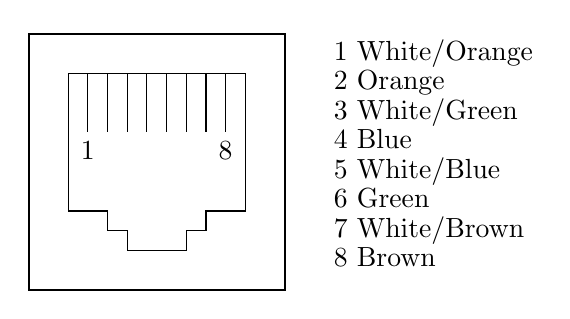
\begin{tikzpicture}[scale=.25]
	\draw [thick] (0,0) -- (0,13) -- (13,13) -- (13,0) -- cycle;
	\draw (2,11) -- (11,11) -- (11,4) -- (9,4) -- (9,3) -- (8,3) -- (8,2) -- (5,2) -- (5,3) -- (4,3) -- (4,4) -- (2,4) -- cycle;
	\foreach \x in {3, 4, 5, 6, 7, 8, 9, 10} {
		\draw (\x,11) -- (\x,8);
	}
	\node [below] at (3,8) {1};
	\node [below] at (10,8) {8};
	\node [right] at (15,12) {\strut 1 White/Orange};
	\node [right] at (15,10.5) {\strut 2 Orange};
	\node [right] at (15,9) {\strut 3 White/Green};
	\node [right] at (15,7.5)  {\strut 4 Blue};
	\node [right] at (15,6)  {\strut 5 White/Blue};
	\node [right] at (15,4.5)  {\strut 6 Green};
	\node [right] at (15,3)  {\strut 7 White/Brown};
	\node [right] at (15,1.5)  {\strut 8 Brown};
\end{tikzpicture}
	\caption{Female 8p8c Modular Jack with T-568B Color Codes\label{fig:8p8c}}
\end{center}
\end{figure}

\subsection{Lumos Wiring Pinout}
The author's personal wiring standard used by all his \acronym{RS-485}-capable projects, staring with Lumos, supports full-duplex communication (i.e., a data pair that is dedicated
to signals from the host PC out to all the connected units---but which could reverse direction if used with half-duplex devices---and a return data pair dedicated to signals from
the networked devices back to the host) and a cable-check pair which can be used to power very small devices such as the Busylight or to verify that the entire set of daisy-chained
devices are all fully connected and terminated.

The pinout is as follows:
\begin{center}
\begin{tabular}{cl}\toprule
	\bfseries Pin & \bfseries Signal\\\midrule
	1&Return data A (+)\\
	2&Return data B (--)\\
	3&Cable check send (outbound +9--16\,V)\\
	4&Data B (--)\\
	5&Data A (+)\\
	6&Cable check return\\
	7&Ground\\
	8&Ground\\\bottomrule
\end{tabular}
\end{center}

\subsection{9-pin Connectors}
Some applications use a \acronym{DE-9} connector\footnote{Also commonly, but incorrectly, called ``DB-9'' connectors.} for \acronym{RS-485} signals, with pinouts such as:
\begin{center}
	\begin{tabular}{cl}\toprule
		\bfseries Pin & \bfseries Signal\\\midrule
		1&Ground\\
		2&Clear to Send (CTS) +\\
		3&Request to Send (RTS) +\\
		4&Received Data (RxD) +\\
		5&Received Data (RxD) --\\
		6&Clear to Send (CTS) --\\
		7&Request to Send (RTS) --\\
		8&Transmitted Data (TxD) +\\
		9&Transmitted Data (TxD) --\\
		\bottomrule
	\end{tabular}
\end{center}

\section{DIN-8 Busylight Tree Connectors}
The Busylight control boards use a \acronym{DIN-8} jack where the light tree cable plugs in to carry the light-signal
voltages out to the light tree itself. The pinout used is:
\begin{figure}
	\begin{center}
		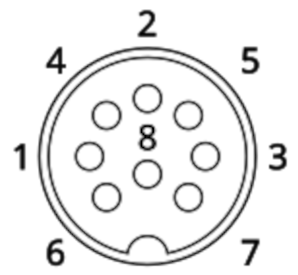
\includegraphics[width=1in]{images/din8.png}\\
		{\tiny Image: adapted from original by Ancillalover, Wikimedia Commons, CC-BY-SA 4.0 int'l.}
		\caption{DIN-8 Jack (looking into socket from front)\label{fig:din9}}
	\end{center}
\end{figure}
\begin{center}
	\begin{tabular}{ccll}\toprule
		\bfseries Pin & \bfseries Tier & \bfseries Light Color & \bfseries Wire Color\\\midrule
		1&6&blue&blue\\
		2&3&amber&white/brown\\
		3&5&red&white/orange\\
		4&4&red&orange\\
		5&7&white&white/blue\\
		6&2&amber&brown\\
		7&&+5\,V power&green\\
		8&1&green&white/green\\\bottomrule
	\end{tabular}
\end{center}


\section{Connectors for Version 3.3 Boards}
\subsection{Arduino Bus Connectors [J0]}
Two parallel rows of stacking pins, for a total of 50 pins, extend out of the back of the readerboard \acronym{PCB}.
An Arduino Mega 2560 or Due microcontroller board is connected to these pins.

The \acronym{USB} connector on the Arduino board may be used to directly connect the readerboard to a \acronym{PC}
for initial configuration and/or to use it as a directly-connected singleton device. (If there are multiple
devices in use, it may be preferable to switch to the \acronym{RS-485} network after initial configuration of the
device.)

\subsection{Version 3.3.1 Boards}
The external connections changed significantly at revision 3.3.1. Now J1 is a pair of push-in terminal
blocks with a combined total of 16 wire connections to make it easy to connect a pair of \acronym{CAT6} cables
(cable ``A'' which carries the incoming data signals, and cable ``B'' which carries the same signals out to
the next daisy-chained unit on the \acronym{RS-485} serial network). The expanded terminal block eliminates the
need to make off-board connections or splices between the cables.

The terminals are labeled as ``A1'' (cable A, pin 1), ``B2'' (cable B, pin 2) and so forth:
\begin{center}
	\begin{tabular}{rcl|rcl}\toprule
		\bfseries Pin & \bfseries Wire & \bfseries Signal &
		\bfseries Pin & \bfseries Wire & \bfseries Signal \\\midrule
		1&A1&Return Data A(+) In*   & 9&A7&Ground In\\
		2&B1&Return Data A(+) Out*  &10&B7&Ground Out\\
		3&A2&Return Data B(--) In*  &11&A8&Ground In\\
		4&B2&Return Data B(--) Out* &12&B8&Ground Out\\
		5&A3&Cable Check Send + In* &13&A5&Data A(+) In\\
		6&B3&Cable Check Send + Out*&14&B5&Data A(+) Out\\
		7&A6&Cable Check Return In* &15&A4&Data B(--) In\\
		8&B6&Cable Check Return Out*&16&B4&Data B(--) Out\\
		\bottomrule
		\multicolumn{6}{l}{*Signal not used by the readerboard unit (passed through).}
	\end{tabular}
\end{center}

If this device is the last in the RS-485 network chain, insert a 120$\Omega$ resistor between the A and B terminals
that would have been used as the output if there had been another device connected there (e.g., B4 and B5). This properly terminates
the RS-485 network at that point.

The power supply to the readerboard unit is on terminal block J5, with +9\,V~DC and ground connections as marked
on the board.

\subsection{Version 3.3.0 Boards}
The previous revision, 3.3.0, used a single terminal block J1 to carry the power supply and the \acronym{RS-485} signals
we actually use, leaving the other wires of the serial cables to be connected externally.

The single external connector on version 3.3.0 boards is an 8-pin screw terminal block. This accepts a +9\,V DC power input
and ground on pins 8 and 7 respectively, which powers the entire board and the attached Arduino controller.  If RS-485
communications will be used, the incoming signal is received on pins 1, 2, and 6 while the outgoing signal is on
pins 3, 4, and 5. (In actuality, the ``input'' and ``output'' sense is arbitrary and either set of A and B signals
may be used as input or output.) 

If this device is the last in the RS-485 network chain, insert a 120$\Omega$ resistor between the A and B terminals
that would have been used as the output if there had been another device connected there. This properly terminates
the RS-485 network at that point.
\begin{center}
	\begin{tabular}{rl|rl}\toprule
		\bfseries Pin & \bfseries Signal &
		\bfseries Pin & \bfseries Signal \\\midrule
		1&A (Data in +)    &5&GND\\
		2&B (Data in --)   &6&GND\\
		3&A (Data out +)   &7&GND\\
		4&B (Data out --)  &8&+9\,V DC in\\\bottomrule
	\end{tabular}
\end{center}

The pinout of J1 for revision 3.2.2 boards is different:
\begin{center}
	\begin{tabular}{rl|rl}\toprule
		\bfseries Pin & \bfseries Signal &
		\bfseries Pin & \bfseries Signal \\\midrule
		1&A (Data in +)    &5&GND\\
		2&B (Data in --)   &6&GND\\
		3&+9\,V DC in      &7&A (Data out +)\\
		4&GND              &8&B (Data out --)\\\bottomrule
	\end{tabular}
\end{center}

{\color{gray}
\section{Connectors for Legacy Boards}
\subsection{Connectors for Version 2.1 Boards}
\subsubsection{Power / RS-485 (8-pin terminal) [J0]}
This is wired the same as J1 on the revision 3.2 boards.
\subsection{Earlier Boards}
\subsubsection{Matrix Control (24-pin ribbon cable) [J1]}
%
%   . . . . . . . . . . . . .
%   . . . . . . . . . . . . .
%
\begin{center}
	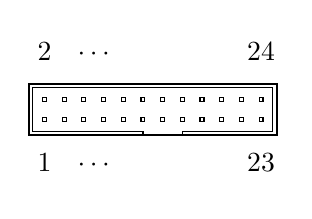
\begin{tikzpicture}[scale=.25]
		\foreach \x in {1, 2, 3, 4, 5, 6, 7, 8, 9, 10, 11, 12} {
			\foreach \y in {1, 2} {
				\draw (\x-.1,\y-.1) -- (\x-.1,\y+.1) -- (\x+.1,\y+.1) -- (\x+.1,\y-.1) -- cycle;
			}
		}
		%\draw         (.4,.4) -- (.4,2.6) -- (13.6,2.6) -- (13.6,.4) -- (.4,.4);
		\draw         (.4,.4) -- (.4,2.6) -- (12.6,2.6) -- (12.6,.4) -- (8,.4) -- (8,.2) -- (6,.2) -- (6,.4) -- cycle;
		\draw [thick] (.2,.2) -- (.2,2.8) -- (12.8,2.8) -- (12.8,.2) -- cycle;
		\node [below] at (1,0) {\strut1};
		\node [above] at (1,3) {\strut2};
%		\node [below] at (2,0) {\strut3};
%		\node [above] at (2,3) {\strut4};
		\node [below] at (3.5,0) {\strut$\cdots$};
		\node [above] at (3.5,3) {\strut$\cdots$};
		\node [below] at (12,0) {\strut 23};
		\node [above] at (12,3) {\strut 24};
	\end{tikzpicture}
\end{center}
For readerboards before version 2.1.0, this 24-position ribbon cable carries signals to directly drive the 64$\times$8 \led\
matrix.  The other end of this cable mates with J0 on the shield board. The pinout of its \acronym{IDC} header  is:
\begin{center}
	\begin{tabular}{rl|rl|rl|rl}
		1&D6     & 7&RCLK                          &13&+5\,V DC&19&Gnd\\
		2&D5     & 8&D2                            &14&+5\,V DC&20&Gnd\\
		3&D7     & 9&$\overline{\hbox{\mc{G}}}$    &15&+5\,V DC&21&R2\\
		4&D4     &10&D1                            &16&+5\,V DC&22&REN\\
		5&SRCLK  &11&$\overline{\hbox{\mc{SRCLR}}}$&17&Gnd     &23&R1\\
		6&D3     &12&D0                            &18&Gnd     &24&R0\\
	\end{tabular}
\end{center}
\subsubsection{Discrete LEDs (10-pin ribbon cable) [J2]}
%
%   . . . . . . . . . . . . .
%   . . . . . . . . . . . . .
%
\begin{center}
	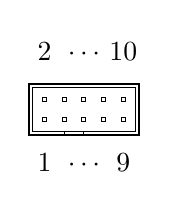
\begin{tikzpicture}[scale=.25]
		\foreach \x in {1, 2, 3, 4, 5} {
			\foreach \y in {1, 2} {
				\draw (\x-.1,\y-.1) -- (\x-.1,\y+.1) -- (\x+.1,\y+.1) -- (\x+.1,\y-.1) -- cycle;
			}
		}
		%\draw         (.4,.4) -- (.4,2.6) -- (13.6,2.6) -- (13.6,.4) -- (.4,.4);
		\draw         (.4,.4) -- (.4,2.6) -- (5.6,2.6) -- (5.6,.4) -- (2,.4) -- (2,.2) -- (3,.2) -- (3,.4) -- cycle;
		\draw [thick] (.2,.2) -- (.2,2.8) -- (5.8,2.8) -- (5.8,.2) -- cycle;
		\node [below] at (1,0) {\strut1};
		\node [above] at (1,3) {\strut2};
%		\node [below] at (2,0) {\strut3};
%		\node [above] at (2,3) {\strut4};
		\node [below] at (3,0) {\strut$\cdots$};
		\node [above] at (3,3) {\strut$\cdots$};
		\node [below] at (5,0) {\strut 9};
		\node [above] at (5,3) {\strut 10};
	\end{tikzpicture}
\end{center}
For readerboards before version 2.1.0, this 10-position ribbon cable carries signals to directly drive the 64$\times$8 \led\
matrix.  The other end of the cable mates with J1 on the shield board. The pinout of its \acronym{IDC} header  is:
\begin{center}
	\begin{tabular}{rl|rl}
		1&GND& 6&L6\\
		2&GND& 7&L2\\
		3&L0 & 8&L5\\
		4&L7 & 9&L3\\
		5&L1 &10&L4\\
	\end{tabular}
\end{center}
\subsubsection{Board Power (3-pin screw terminal) [J0]}
This 3-position screw terminal block provides power to the readerboard. Note that the +5\,V supply is also connected
to pins 13--16, and Ground to pins 17--20 of J1, the only power required here is the +9\,V input that drives the \led s themselves.
\begin{center}
	\begin{tabular}{rl}
		1&+5\,V DC in\\
		2&GND\\
		3&+9\,V DC in\\
	\end{tabular}
\end{center}

\subsubsection{Shield Power (5-pin screw terminal) [Shield J2]}
This 5-position screw terminal block accepts incoming +9\,V DC power and ground on pins 4 and 3 respectively. It then provides
+5\,V DC, +9\,V DC, and ground outputs on pins 1, 2, and 5 respectively to supply power to the main display board.
\begin{center}
	\begin{tabular}{rl}
		1&+5\,V DC out\\
		2&GND\\
		3&GND\\
		4&+9\,V DC in\\
		5&+9\,V DC out\\
	\end{tabular}
\end{center}

\subsubsection{Shield RS-485 (6-pin screw terminal) [Shield J4]}
This 6-position screw terminal block accepts incoming RS-485 signals A, B, and ground on pins 2, 1, and 3 respectively, and outputs
the network signals A, B, and ground on pins 6, 5, and 4 respectively, to go on to the next device in the chain. If this is the last
device, then nothing should be connected to pins 5 and 6. Instead, install jumper J5 which connects a 120$\Omega$ resistor across
those terminals to terminate the network at that point.
\begin{center}
	\begin{tabular}{rl}
		1&B (Data In --)\\
		2&A (Data In +)\\
		3&GND\\
		4&GND\\
		5&B (Data Out --)\\
		6&A (Data Out +)\\
	\end{tabular}
\end{center}
}

%%%%%%%%%%%%%%%%%%%%%%%%%%%%%%%%%%%%%%%%%%%%%%%%%%%%%%%%%%%%%%%%%%%%%%%%%%%%%%%%%%%%%%%%%%%%%%%%%%%%
%  ___ _   _ ____ _____  _    _     _     ___ _   _  ____ 
% |_ _| \ | / ___|_   _|/ \  | |   | |   |_ _| \ | |/ ___|
%  | ||  \| \___ \ | | / _ \ | |   | |    | ||  \| | |  _ 
%  | || |\  |___) || |/ ___ \| |___| |___ | || |\  | |_| |
% |___|_| \_|____/ |_/_/   \_\_____|_____|___|_| \_|\____|
%                                                         
\chapter{Installing and Using the Readerboard and Busylight Units}
\epigraph{See, unlike most hackers, I get little joy out of figuring out how to install the latest toy.}{---Jamie Zawinski}
\section{Standalone Units}
\section{Networked Units}
\section{Compiling the Supporting Software}
\section{Setting up \z{rbserver}}
\section{Setting up Per-User Utilities}
\subsection{\z{calmond}}
\subsection{\z{micmond}}
\subsection{Manual Status Updates}
\section{Diagnostic Displays}
There are a few situations where the readerboards and busylights use their light displays to convey
information about their own status.

\subsection{EEPROM Access}
When a readerboard accesses its \acronym{EEPROM}, a small superscripted ``\strut$^{EE}$'' is displayed
in the upper-right corner of the matrix. The next update to the displayed matrix content will overwrite
this indicator. The color of the indicator indicates the type or outcome of the operation:
\begin{center}
	\begin{tabular}{lll}\toprule
		\bfseries RGB Units & \bfseries Monochrome Units & \bfseries Meaning\\\midrule
		green & on & reading \\
		yellow & on & writing \\
		flashing red & flashing & error \\
		\bottomrule
	\end{tabular}
\end{center}

\subsection{Protocol Errors}
If the device receives garbled or otherwise incorrect commands over either \acronym{USB} or \acronym{RS-485},
it lights the top discrete status \led\ and alternately strobes the fourth and fifth from the bottom. On units with our
standard color scheme, this is the white and both red \led s. 

These will be displayed until the next status \led\ command changes them.

\subsection{POST}
During power-on self-test when a readerboard is turned on, the top (usually white) \led\ is illuminated until the \acronym{POST} operation is completed.

%%%%%%%%%%%%%%%%%%%%%%%%%%%%%%%%%%%%%%%%%%%%%%%%%%%%%%%%%%%%%%%%%%%%%%%%%%%%%%%%%%%%%%%%%%%%%%%%%%%%
%  _____ ___  _   _ _____ ____  
% |  ___/ _ \| \ | |_   _/ ___| 
% | |_ | | | |  \| | | | \___ \ 
% |  _|| |_| | |\  | | |  ___) |
% |_|   \___/|_| \_| |_| |____/ 
%                               
\chapter{Font Glyphs}\label{chap:fonts}
\epigraph{Helvetica is the sweatpants of typefaces.}{---John Boardley}
\section{Font \#0 \z{standard.font}}
% font 0 codepoint 32 name space space 6 width 0 offset 5
\noindent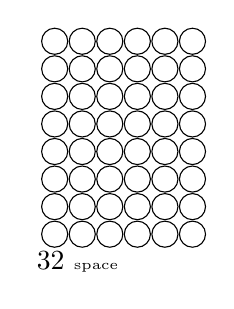
\begin{tikzpicture}[x=3.5mm,y=3.5mm]
\node [right] at (0,0) {32 {\tiny space}};
\node [circle, fill=none, draw=black, minimum size=3mm] at (1,8) {};
\node [circle, fill=none, draw=black, minimum size=3mm] at (2,8) {};
\node [circle, fill=none, draw=black, minimum size=3mm] at (3,8) {};
\node [circle, fill=none, draw=black, minimum size=3mm] at (4,8) {};
\node [circle, fill=none, draw=black, minimum size=3mm] at (5,8) {};
\node [circle, fill=none, draw=black, minimum size=3mm] at (6,8) {};
\node [circle, fill=none, draw=black, minimum size=3mm] at (1,7) {};
\node [circle, fill=none, draw=black, minimum size=3mm] at (2,7) {};
\node [circle, fill=none, draw=black, minimum size=3mm] at (3,7) {};
\node [circle, fill=none, draw=black, minimum size=3mm] at (4,7) {};
\node [circle, fill=none, draw=black, minimum size=3mm] at (5,7) {};
\node [circle, fill=none, draw=black, minimum size=3mm] at (6,7) {};
\node [circle, fill=none, draw=black, minimum size=3mm] at (1,6) {};
\node [circle, fill=none, draw=black, minimum size=3mm] at (2,6) {};
\node [circle, fill=none, draw=black, minimum size=3mm] at (3,6) {};
\node [circle, fill=none, draw=black, minimum size=3mm] at (4,6) {};
\node [circle, fill=none, draw=black, minimum size=3mm] at (5,6) {};
\node [circle, fill=none, draw=black, minimum size=3mm] at (6,6) {};
\node [circle, fill=none, draw=black, minimum size=3mm] at (1,5) {};
\node [circle, fill=none, draw=black, minimum size=3mm] at (2,5) {};
\node [circle, fill=none, draw=black, minimum size=3mm] at (3,5) {};
\node [circle, fill=none, draw=black, minimum size=3mm] at (4,5) {};
\node [circle, fill=none, draw=black, minimum size=3mm] at (5,5) {};
\node [circle, fill=none, draw=black, minimum size=3mm] at (6,5) {};
\node [circle, fill=none, draw=black, minimum size=3mm] at (1,4) {};
\node [circle, fill=none, draw=black, minimum size=3mm] at (2,4) {};
\node [circle, fill=none, draw=black, minimum size=3mm] at (3,4) {};
\node [circle, fill=none, draw=black, minimum size=3mm] at (4,4) {};
\node [circle, fill=none, draw=black, minimum size=3mm] at (5,4) {};
\node [circle, fill=none, draw=black, minimum size=3mm] at (6,4) {};
\node [circle, fill=none, draw=black, minimum size=3mm] at (1,3) {};
\node [circle, fill=none, draw=black, minimum size=3mm] at (2,3) {};
\node [circle, fill=none, draw=black, minimum size=3mm] at (3,3) {};
\node [circle, fill=none, draw=black, minimum size=3mm] at (4,3) {};
\node [circle, fill=none, draw=black, minimum size=3mm] at (5,3) {};
\node [circle, fill=none, draw=black, minimum size=3mm] at (6,3) {};
\node [circle, fill=none, draw=black, minimum size=3mm] at (1,2) {};
\node [circle, fill=none, draw=black, minimum size=3mm] at (2,2) {};
\node [circle, fill=none, draw=black, minimum size=3mm] at (3,2) {};
\node [circle, fill=none, draw=black, minimum size=3mm] at (4,2) {};
\node [circle, fill=none, draw=black, minimum size=3mm] at (5,2) {};
\node [circle, fill=none, draw=black, minimum size=3mm] at (6,2) {};
\node [circle, fill=none, draw=black, minimum size=3mm] at (1,1) {};
\node [circle, fill=none, draw=black, minimum size=3mm] at (2,1) {};
\node [circle, fill=none, draw=black, minimum size=3mm] at (3,1) {};
\node [circle, fill=none, draw=black, minimum size=3mm] at (4,1) {};
\node [circle, fill=none, draw=black, minimum size=3mm] at (5,1) {};
\node [circle, fill=none, draw=black, minimum size=3mm] at (6,1) {};
\end{tikzpicture}% font 0 codepoint 33 name exclamation space 6 width 3 offset 5
~ 
\noindent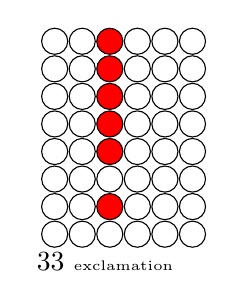
\begin{tikzpicture}[x=3.5mm,y=3.5mm]
\node [right] at (0,0) {33 {\tiny exclamation}};
\node [circle, fill=none, draw=black, minimum size=3mm] at (1,8) {};
\node [circle, fill=none, draw=black, minimum size=3mm] at (2,8) {};
\node [circle, fill=red, draw=black, minimum size=3mm] at (3,8) {};
\node [circle, fill=none, draw=black, minimum size=3mm] at (4,8) {};
\node [circle, fill=none, draw=black, minimum size=3mm] at (5,8) {};
\node [circle, fill=none, draw=black, minimum size=3mm] at (6,8) {};
\node [circle, fill=none, draw=black, minimum size=3mm] at (1,7) {};
\node [circle, fill=none, draw=black, minimum size=3mm] at (2,7) {};
\node [circle, fill=red, draw=black, minimum size=3mm] at (3,7) {};
\node [circle, fill=none, draw=black, minimum size=3mm] at (4,7) {};
\node [circle, fill=none, draw=black, minimum size=3mm] at (5,7) {};
\node [circle, fill=none, draw=black, minimum size=3mm] at (6,7) {};
\node [circle, fill=none, draw=black, minimum size=3mm] at (1,6) {};
\node [circle, fill=none, draw=black, minimum size=3mm] at (2,6) {};
\node [circle, fill=red, draw=black, minimum size=3mm] at (3,6) {};
\node [circle, fill=none, draw=black, minimum size=3mm] at (4,6) {};
\node [circle, fill=none, draw=black, minimum size=3mm] at (5,6) {};
\node [circle, fill=none, draw=black, minimum size=3mm] at (6,6) {};
\node [circle, fill=none, draw=black, minimum size=3mm] at (1,5) {};
\node [circle, fill=none, draw=black, minimum size=3mm] at (2,5) {};
\node [circle, fill=red, draw=black, minimum size=3mm] at (3,5) {};
\node [circle, fill=none, draw=black, minimum size=3mm] at (4,5) {};
\node [circle, fill=none, draw=black, minimum size=3mm] at (5,5) {};
\node [circle, fill=none, draw=black, minimum size=3mm] at (6,5) {};
\node [circle, fill=none, draw=black, minimum size=3mm] at (1,4) {};
\node [circle, fill=none, draw=black, minimum size=3mm] at (2,4) {};
\node [circle, fill=red, draw=black, minimum size=3mm] at (3,4) {};
\node [circle, fill=none, draw=black, minimum size=3mm] at (4,4) {};
\node [circle, fill=none, draw=black, minimum size=3mm] at (5,4) {};
\node [circle, fill=none, draw=black, minimum size=3mm] at (6,4) {};
\node [circle, fill=none, draw=black, minimum size=3mm] at (1,3) {};
\node [circle, fill=none, draw=black, minimum size=3mm] at (2,3) {};
\node [circle, fill=none, draw=black, minimum size=3mm] at (3,3) {};
\node [circle, fill=none, draw=black, minimum size=3mm] at (4,3) {};
\node [circle, fill=none, draw=black, minimum size=3mm] at (5,3) {};
\node [circle, fill=none, draw=black, minimum size=3mm] at (6,3) {};
\node [circle, fill=none, draw=black, minimum size=3mm] at (1,2) {};
\node [circle, fill=none, draw=black, minimum size=3mm] at (2,2) {};
\node [circle, fill=red, draw=black, minimum size=3mm] at (3,2) {};
\node [circle, fill=none, draw=black, minimum size=3mm] at (4,2) {};
\node [circle, fill=none, draw=black, minimum size=3mm] at (5,2) {};
\node [circle, fill=none, draw=black, minimum size=3mm] at (6,2) {};
\node [circle, fill=none, draw=black, minimum size=3mm] at (1,1) {};
\node [circle, fill=none, draw=black, minimum size=3mm] at (2,1) {};
\node [circle, fill=none, draw=black, minimum size=3mm] at (3,1) {};
\node [circle, fill=none, draw=black, minimum size=3mm] at (4,1) {};
\node [circle, fill=none, draw=black, minimum size=3mm] at (5,1) {};
\node [circle, fill=none, draw=black, minimum size=3mm] at (6,1) {};
\end{tikzpicture}% font 0 codepoint 34 name quotation mark space 6 width 4 offset 8
~ 
\noindent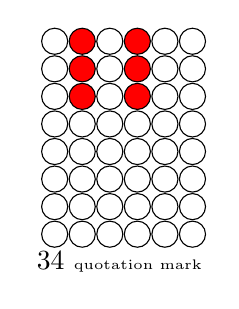
\begin{tikzpicture}[x=3.5mm,y=3.5mm]
\node [right] at (0,0) {34 {\tiny quotation mark}};
\node [circle, fill=none, draw=black, minimum size=3mm] at (1,8) {};
\node [circle, fill=red, draw=black, minimum size=3mm] at (2,8) {};
\node [circle, fill=none, draw=black, minimum size=3mm] at (3,8) {};
\node [circle, fill=red, draw=black, minimum size=3mm] at (4,8) {};
\node [circle, fill=none, draw=black, minimum size=3mm] at (5,8) {};
\node [circle, fill=none, draw=black, minimum size=3mm] at (6,8) {};
\node [circle, fill=none, draw=black, minimum size=3mm] at (1,7) {};
\node [circle, fill=red, draw=black, minimum size=3mm] at (2,7) {};
\node [circle, fill=none, draw=black, minimum size=3mm] at (3,7) {};
\node [circle, fill=red, draw=black, minimum size=3mm] at (4,7) {};
\node [circle, fill=none, draw=black, minimum size=3mm] at (5,7) {};
\node [circle, fill=none, draw=black, minimum size=3mm] at (6,7) {};
\node [circle, fill=none, draw=black, minimum size=3mm] at (1,6) {};
\node [circle, fill=red, draw=black, minimum size=3mm] at (2,6) {};
\node [circle, fill=none, draw=black, minimum size=3mm] at (3,6) {};
\node [circle, fill=red, draw=black, minimum size=3mm] at (4,6) {};
\node [circle, fill=none, draw=black, minimum size=3mm] at (5,6) {};
\node [circle, fill=none, draw=black, minimum size=3mm] at (6,6) {};
\node [circle, fill=none, draw=black, minimum size=3mm] at (1,5) {};
\node [circle, fill=none, draw=black, minimum size=3mm] at (2,5) {};
\node [circle, fill=none, draw=black, minimum size=3mm] at (3,5) {};
\node [circle, fill=none, draw=black, minimum size=3mm] at (4,5) {};
\node [circle, fill=none, draw=black, minimum size=3mm] at (5,5) {};
\node [circle, fill=none, draw=black, minimum size=3mm] at (6,5) {};
\node [circle, fill=none, draw=black, minimum size=3mm] at (1,4) {};
\node [circle, fill=none, draw=black, minimum size=3mm] at (2,4) {};
\node [circle, fill=none, draw=black, minimum size=3mm] at (3,4) {};
\node [circle, fill=none, draw=black, minimum size=3mm] at (4,4) {};
\node [circle, fill=none, draw=black, minimum size=3mm] at (5,4) {};
\node [circle, fill=none, draw=black, minimum size=3mm] at (6,4) {};
\node [circle, fill=none, draw=black, minimum size=3mm] at (1,3) {};
\node [circle, fill=none, draw=black, minimum size=3mm] at (2,3) {};
\node [circle, fill=none, draw=black, minimum size=3mm] at (3,3) {};
\node [circle, fill=none, draw=black, minimum size=3mm] at (4,3) {};
\node [circle, fill=none, draw=black, minimum size=3mm] at (5,3) {};
\node [circle, fill=none, draw=black, minimum size=3mm] at (6,3) {};
\node [circle, fill=none, draw=black, minimum size=3mm] at (1,2) {};
\node [circle, fill=none, draw=black, minimum size=3mm] at (2,2) {};
\node [circle, fill=none, draw=black, minimum size=3mm] at (3,2) {};
\node [circle, fill=none, draw=black, minimum size=3mm] at (4,2) {};
\node [circle, fill=none, draw=black, minimum size=3mm] at (5,2) {};
\node [circle, fill=none, draw=black, minimum size=3mm] at (6,2) {};
\node [circle, fill=none, draw=black, minimum size=3mm] at (1,1) {};
\node [circle, fill=none, draw=black, minimum size=3mm] at (2,1) {};
\node [circle, fill=none, draw=black, minimum size=3mm] at (3,1) {};
\node [circle, fill=none, draw=black, minimum size=3mm] at (4,1) {};
\node [circle, fill=none, draw=black, minimum size=3mm] at (5,1) {};
\node [circle, fill=none, draw=black, minimum size=3mm] at (6,1) {};
\end{tikzpicture}% font 0 codepoint 35 name pound sign space 6 width 5 offset 12
~ 
\noindent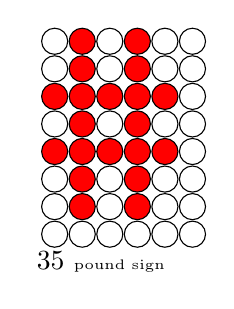
\begin{tikzpicture}[x=3.5mm,y=3.5mm]
\node [right] at (0,0) {35 {\tiny pound sign}};
\node [circle, fill=none, draw=black, minimum size=3mm] at (1,8) {};
\node [circle, fill=red, draw=black, minimum size=3mm] at (2,8) {};
\node [circle, fill=none, draw=black, minimum size=3mm] at (3,8) {};
\node [circle, fill=red, draw=black, minimum size=3mm] at (4,8) {};
\node [circle, fill=none, draw=black, minimum size=3mm] at (5,8) {};
\node [circle, fill=none, draw=black, minimum size=3mm] at (6,8) {};
\node [circle, fill=none, draw=black, minimum size=3mm] at (1,7) {};
\node [circle, fill=red, draw=black, minimum size=3mm] at (2,7) {};
\node [circle, fill=none, draw=black, minimum size=3mm] at (3,7) {};
\node [circle, fill=red, draw=black, minimum size=3mm] at (4,7) {};
\node [circle, fill=none, draw=black, minimum size=3mm] at (5,7) {};
\node [circle, fill=none, draw=black, minimum size=3mm] at (6,7) {};
\node [circle, fill=red, draw=black, minimum size=3mm] at (1,6) {};
\node [circle, fill=red, draw=black, minimum size=3mm] at (2,6) {};
\node [circle, fill=red, draw=black, minimum size=3mm] at (3,6) {};
\node [circle, fill=red, draw=black, minimum size=3mm] at (4,6) {};
\node [circle, fill=red, draw=black, minimum size=3mm] at (5,6) {};
\node [circle, fill=none, draw=black, minimum size=3mm] at (6,6) {};
\node [circle, fill=none, draw=black, minimum size=3mm] at (1,5) {};
\node [circle, fill=red, draw=black, minimum size=3mm] at (2,5) {};
\node [circle, fill=none, draw=black, minimum size=3mm] at (3,5) {};
\node [circle, fill=red, draw=black, minimum size=3mm] at (4,5) {};
\node [circle, fill=none, draw=black, minimum size=3mm] at (5,5) {};
\node [circle, fill=none, draw=black, minimum size=3mm] at (6,5) {};
\node [circle, fill=red, draw=black, minimum size=3mm] at (1,4) {};
\node [circle, fill=red, draw=black, minimum size=3mm] at (2,4) {};
\node [circle, fill=red, draw=black, minimum size=3mm] at (3,4) {};
\node [circle, fill=red, draw=black, minimum size=3mm] at (4,4) {};
\node [circle, fill=red, draw=black, minimum size=3mm] at (5,4) {};
\node [circle, fill=none, draw=black, minimum size=3mm] at (6,4) {};
\node [circle, fill=none, draw=black, minimum size=3mm] at (1,3) {};
\node [circle, fill=red, draw=black, minimum size=3mm] at (2,3) {};
\node [circle, fill=none, draw=black, minimum size=3mm] at (3,3) {};
\node [circle, fill=red, draw=black, minimum size=3mm] at (4,3) {};
\node [circle, fill=none, draw=black, minimum size=3mm] at (5,3) {};
\node [circle, fill=none, draw=black, minimum size=3mm] at (6,3) {};
\node [circle, fill=none, draw=black, minimum size=3mm] at (1,2) {};
\node [circle, fill=red, draw=black, minimum size=3mm] at (2,2) {};
\node [circle, fill=none, draw=black, minimum size=3mm] at (3,2) {};
\node [circle, fill=red, draw=black, minimum size=3mm] at (4,2) {};
\node [circle, fill=none, draw=black, minimum size=3mm] at (5,2) {};
\node [circle, fill=none, draw=black, minimum size=3mm] at (6,2) {};
\node [circle, fill=none, draw=black, minimum size=3mm] at (1,1) {};
\node [circle, fill=none, draw=black, minimum size=3mm] at (2,1) {};
\node [circle, fill=none, draw=black, minimum size=3mm] at (3,1) {};
\node [circle, fill=none, draw=black, minimum size=3mm] at (4,1) {};
\node [circle, fill=none, draw=black, minimum size=3mm] at (5,1) {};
\node [circle, fill=none, draw=black, minimum size=3mm] at (6,1) {};
\end{tikzpicture}% font 0 codepoint 36 name dollar sign space 6 width 5 offset 17
~ 
\noindent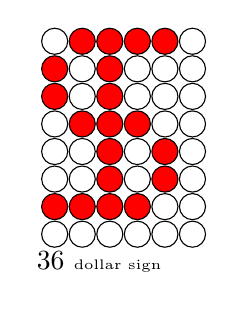
\begin{tikzpicture}[x=3.5mm,y=3.5mm]
\node [right] at (0,0) {36 {\tiny dollar sign}};
\node [circle, fill=none, draw=black, minimum size=3mm] at (1,8) {};
\node [circle, fill=red, draw=black, minimum size=3mm] at (2,8) {};
\node [circle, fill=red, draw=black, minimum size=3mm] at (3,8) {};
\node [circle, fill=red, draw=black, minimum size=3mm] at (4,8) {};
\node [circle, fill=red, draw=black, minimum size=3mm] at (5,8) {};
\node [circle, fill=none, draw=black, minimum size=3mm] at (6,8) {};
\node [circle, fill=red, draw=black, minimum size=3mm] at (1,7) {};
\node [circle, fill=none, draw=black, minimum size=3mm] at (2,7) {};
\node [circle, fill=red, draw=black, minimum size=3mm] at (3,7) {};
\node [circle, fill=none, draw=black, minimum size=3mm] at (4,7) {};
\node [circle, fill=none, draw=black, minimum size=3mm] at (5,7) {};
\node [circle, fill=none, draw=black, minimum size=3mm] at (6,7) {};
\node [circle, fill=red, draw=black, minimum size=3mm] at (1,6) {};
\node [circle, fill=none, draw=black, minimum size=3mm] at (2,6) {};
\node [circle, fill=red, draw=black, minimum size=3mm] at (3,6) {};
\node [circle, fill=none, draw=black, minimum size=3mm] at (4,6) {};
\node [circle, fill=none, draw=black, minimum size=3mm] at (5,6) {};
\node [circle, fill=none, draw=black, minimum size=3mm] at (6,6) {};
\node [circle, fill=none, draw=black, minimum size=3mm] at (1,5) {};
\node [circle, fill=red, draw=black, minimum size=3mm] at (2,5) {};
\node [circle, fill=red, draw=black, minimum size=3mm] at (3,5) {};
\node [circle, fill=red, draw=black, minimum size=3mm] at (4,5) {};
\node [circle, fill=none, draw=black, minimum size=3mm] at (5,5) {};
\node [circle, fill=none, draw=black, minimum size=3mm] at (6,5) {};
\node [circle, fill=none, draw=black, minimum size=3mm] at (1,4) {};
\node [circle, fill=none, draw=black, minimum size=3mm] at (2,4) {};
\node [circle, fill=red, draw=black, minimum size=3mm] at (3,4) {};
\node [circle, fill=none, draw=black, minimum size=3mm] at (4,4) {};
\node [circle, fill=red, draw=black, minimum size=3mm] at (5,4) {};
\node [circle, fill=none, draw=black, minimum size=3mm] at (6,4) {};
\node [circle, fill=none, draw=black, minimum size=3mm] at (1,3) {};
\node [circle, fill=none, draw=black, minimum size=3mm] at (2,3) {};
\node [circle, fill=red, draw=black, minimum size=3mm] at (3,3) {};
\node [circle, fill=none, draw=black, minimum size=3mm] at (4,3) {};
\node [circle, fill=red, draw=black, minimum size=3mm] at (5,3) {};
\node [circle, fill=none, draw=black, minimum size=3mm] at (6,3) {};
\node [circle, fill=red, draw=black, minimum size=3mm] at (1,2) {};
\node [circle, fill=red, draw=black, minimum size=3mm] at (2,2) {};
\node [circle, fill=red, draw=black, minimum size=3mm] at (3,2) {};
\node [circle, fill=red, draw=black, minimum size=3mm] at (4,2) {};
\node [circle, fill=none, draw=black, minimum size=3mm] at (5,2) {};
\node [circle, fill=none, draw=black, minimum size=3mm] at (6,2) {};
\node [circle, fill=none, draw=black, minimum size=3mm] at (1,1) {};
\node [circle, fill=none, draw=black, minimum size=3mm] at (2,1) {};
\node [circle, fill=none, draw=black, minimum size=3mm] at (3,1) {};
\node [circle, fill=none, draw=black, minimum size=3mm] at (4,1) {};
\node [circle, fill=none, draw=black, minimum size=3mm] at (5,1) {};
\node [circle, fill=none, draw=black, minimum size=3mm] at (6,1) {};
\end{tikzpicture}% font 0 codepoint 37 name percent space 6 width 5 offset 22


\noindent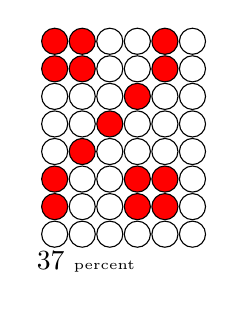
\begin{tikzpicture}[x=3.5mm,y=3.5mm]
\node [right] at (0,0) {37 {\tiny percent}};
\node [circle, fill=red, draw=black, minimum size=3mm] at (1,8) {};
\node [circle, fill=red, draw=black, minimum size=3mm] at (2,8) {};
\node [circle, fill=none, draw=black, minimum size=3mm] at (3,8) {};
\node [circle, fill=none, draw=black, minimum size=3mm] at (4,8) {};
\node [circle, fill=red, draw=black, minimum size=3mm] at (5,8) {};
\node [circle, fill=none, draw=black, minimum size=3mm] at (6,8) {};
\node [circle, fill=red, draw=black, minimum size=3mm] at (1,7) {};
\node [circle, fill=red, draw=black, minimum size=3mm] at (2,7) {};
\node [circle, fill=none, draw=black, minimum size=3mm] at (3,7) {};
\node [circle, fill=none, draw=black, minimum size=3mm] at (4,7) {};
\node [circle, fill=red, draw=black, minimum size=3mm] at (5,7) {};
\node [circle, fill=none, draw=black, minimum size=3mm] at (6,7) {};
\node [circle, fill=none, draw=black, minimum size=3mm] at (1,6) {};
\node [circle, fill=none, draw=black, minimum size=3mm] at (2,6) {};
\node [circle, fill=none, draw=black, minimum size=3mm] at (3,6) {};
\node [circle, fill=red, draw=black, minimum size=3mm] at (4,6) {};
\node [circle, fill=none, draw=black, minimum size=3mm] at (5,6) {};
\node [circle, fill=none, draw=black, minimum size=3mm] at (6,6) {};
\node [circle, fill=none, draw=black, minimum size=3mm] at (1,5) {};
\node [circle, fill=none, draw=black, minimum size=3mm] at (2,5) {};
\node [circle, fill=red, draw=black, minimum size=3mm] at (3,5) {};
\node [circle, fill=none, draw=black, minimum size=3mm] at (4,5) {};
\node [circle, fill=none, draw=black, minimum size=3mm] at (5,5) {};
\node [circle, fill=none, draw=black, minimum size=3mm] at (6,5) {};
\node [circle, fill=none, draw=black, minimum size=3mm] at (1,4) {};
\node [circle, fill=red, draw=black, minimum size=3mm] at (2,4) {};
\node [circle, fill=none, draw=black, minimum size=3mm] at (3,4) {};
\node [circle, fill=none, draw=black, minimum size=3mm] at (4,4) {};
\node [circle, fill=none, draw=black, minimum size=3mm] at (5,4) {};
\node [circle, fill=none, draw=black, minimum size=3mm] at (6,4) {};
\node [circle, fill=red, draw=black, minimum size=3mm] at (1,3) {};
\node [circle, fill=none, draw=black, minimum size=3mm] at (2,3) {};
\node [circle, fill=none, draw=black, minimum size=3mm] at (3,3) {};
\node [circle, fill=red, draw=black, minimum size=3mm] at (4,3) {};
\node [circle, fill=red, draw=black, minimum size=3mm] at (5,3) {};
\node [circle, fill=none, draw=black, minimum size=3mm] at (6,3) {};
\node [circle, fill=red, draw=black, minimum size=3mm] at (1,2) {};
\node [circle, fill=none, draw=black, minimum size=3mm] at (2,2) {};
\node [circle, fill=none, draw=black, minimum size=3mm] at (3,2) {};
\node [circle, fill=red, draw=black, minimum size=3mm] at (4,2) {};
\node [circle, fill=red, draw=black, minimum size=3mm] at (5,2) {};
\node [circle, fill=none, draw=black, minimum size=3mm] at (6,2) {};
\node [circle, fill=none, draw=black, minimum size=3mm] at (1,1) {};
\node [circle, fill=none, draw=black, minimum size=3mm] at (2,1) {};
\node [circle, fill=none, draw=black, minimum size=3mm] at (3,1) {};
\node [circle, fill=none, draw=black, minimum size=3mm] at (4,1) {};
\node [circle, fill=none, draw=black, minimum size=3mm] at (5,1) {};
\node [circle, fill=none, draw=black, minimum size=3mm] at (6,1) {};
\end{tikzpicture}% font 0 codepoint 38 name ampersand space 6 width 5 offset 27
~ 
\noindent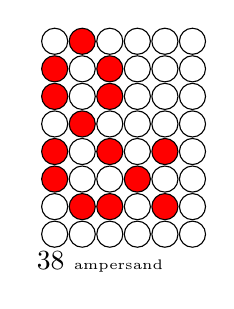
\begin{tikzpicture}[x=3.5mm,y=3.5mm]
\node [right] at (0,0) {38 {\tiny ampersand}};
\node [circle, fill=none, draw=black, minimum size=3mm] at (1,8) {};
\node [circle, fill=red, draw=black, minimum size=3mm] at (2,8) {};
\node [circle, fill=none, draw=black, minimum size=3mm] at (3,8) {};
\node [circle, fill=none, draw=black, minimum size=3mm] at (4,8) {};
\node [circle, fill=none, draw=black, minimum size=3mm] at (5,8) {};
\node [circle, fill=none, draw=black, minimum size=3mm] at (6,8) {};
\node [circle, fill=red, draw=black, minimum size=3mm] at (1,7) {};
\node [circle, fill=none, draw=black, minimum size=3mm] at (2,7) {};
\node [circle, fill=red, draw=black, minimum size=3mm] at (3,7) {};
\node [circle, fill=none, draw=black, minimum size=3mm] at (4,7) {};
\node [circle, fill=none, draw=black, minimum size=3mm] at (5,7) {};
\node [circle, fill=none, draw=black, minimum size=3mm] at (6,7) {};
\node [circle, fill=red, draw=black, minimum size=3mm] at (1,6) {};
\node [circle, fill=none, draw=black, minimum size=3mm] at (2,6) {};
\node [circle, fill=red, draw=black, minimum size=3mm] at (3,6) {};
\node [circle, fill=none, draw=black, minimum size=3mm] at (4,6) {};
\node [circle, fill=none, draw=black, minimum size=3mm] at (5,6) {};
\node [circle, fill=none, draw=black, minimum size=3mm] at (6,6) {};
\node [circle, fill=none, draw=black, minimum size=3mm] at (1,5) {};
\node [circle, fill=red, draw=black, minimum size=3mm] at (2,5) {};
\node [circle, fill=none, draw=black, minimum size=3mm] at (3,5) {};
\node [circle, fill=none, draw=black, minimum size=3mm] at (4,5) {};
\node [circle, fill=none, draw=black, minimum size=3mm] at (5,5) {};
\node [circle, fill=none, draw=black, minimum size=3mm] at (6,5) {};
\node [circle, fill=red, draw=black, minimum size=3mm] at (1,4) {};
\node [circle, fill=none, draw=black, minimum size=3mm] at (2,4) {};
\node [circle, fill=red, draw=black, minimum size=3mm] at (3,4) {};
\node [circle, fill=none, draw=black, minimum size=3mm] at (4,4) {};
\node [circle, fill=red, draw=black, minimum size=3mm] at (5,4) {};
\node [circle, fill=none, draw=black, minimum size=3mm] at (6,4) {};
\node [circle, fill=red, draw=black, minimum size=3mm] at (1,3) {};
\node [circle, fill=none, draw=black, minimum size=3mm] at (2,3) {};
\node [circle, fill=none, draw=black, minimum size=3mm] at (3,3) {};
\node [circle, fill=red, draw=black, minimum size=3mm] at (4,3) {};
\node [circle, fill=none, draw=black, minimum size=3mm] at (5,3) {};
\node [circle, fill=none, draw=black, minimum size=3mm] at (6,3) {};
\node [circle, fill=none, draw=black, minimum size=3mm] at (1,2) {};
\node [circle, fill=red, draw=black, minimum size=3mm] at (2,2) {};
\node [circle, fill=red, draw=black, minimum size=3mm] at (3,2) {};
\node [circle, fill=none, draw=black, minimum size=3mm] at (4,2) {};
\node [circle, fill=red, draw=black, minimum size=3mm] at (5,2) {};
\node [circle, fill=none, draw=black, minimum size=3mm] at (6,2) {};
\node [circle, fill=none, draw=black, minimum size=3mm] at (1,1) {};
\node [circle, fill=none, draw=black, minimum size=3mm] at (2,1) {};
\node [circle, fill=none, draw=black, minimum size=3mm] at (3,1) {};
\node [circle, fill=none, draw=black, minimum size=3mm] at (4,1) {};
\node [circle, fill=none, draw=black, minimum size=3mm] at (5,1) {};
\node [circle, fill=none, draw=black, minimum size=3mm] at (6,1) {};
\end{tikzpicture}% font 0 codepoint 39 name apostrophe space 6 width 3 offset 32
~ 
\noindent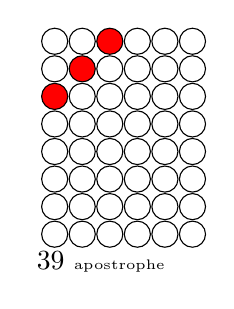
\begin{tikzpicture}[x=3.5mm,y=3.5mm]
\node [right] at (0,0) {39 {\tiny apostrophe}};
\node [circle, fill=none, draw=black, minimum size=3mm] at (1,8) {};
\node [circle, fill=none, draw=black, minimum size=3mm] at (2,8) {};
\node [circle, fill=red, draw=black, minimum size=3mm] at (3,8) {};
\node [circle, fill=none, draw=black, minimum size=3mm] at (4,8) {};
\node [circle, fill=none, draw=black, minimum size=3mm] at (5,8) {};
\node [circle, fill=none, draw=black, minimum size=3mm] at (6,8) {};
\node [circle, fill=none, draw=black, minimum size=3mm] at (1,7) {};
\node [circle, fill=red, draw=black, minimum size=3mm] at (2,7) {};
\node [circle, fill=none, draw=black, minimum size=3mm] at (3,7) {};
\node [circle, fill=none, draw=black, minimum size=3mm] at (4,7) {};
\node [circle, fill=none, draw=black, minimum size=3mm] at (5,7) {};
\node [circle, fill=none, draw=black, minimum size=3mm] at (6,7) {};
\node [circle, fill=red, draw=black, minimum size=3mm] at (1,6) {};
\node [circle, fill=none, draw=black, minimum size=3mm] at (2,6) {};
\node [circle, fill=none, draw=black, minimum size=3mm] at (3,6) {};
\node [circle, fill=none, draw=black, minimum size=3mm] at (4,6) {};
\node [circle, fill=none, draw=black, minimum size=3mm] at (5,6) {};
\node [circle, fill=none, draw=black, minimum size=3mm] at (6,6) {};
\node [circle, fill=none, draw=black, minimum size=3mm] at (1,5) {};
\node [circle, fill=none, draw=black, minimum size=3mm] at (2,5) {};
\node [circle, fill=none, draw=black, minimum size=3mm] at (3,5) {};
\node [circle, fill=none, draw=black, minimum size=3mm] at (4,5) {};
\node [circle, fill=none, draw=black, minimum size=3mm] at (5,5) {};
\node [circle, fill=none, draw=black, minimum size=3mm] at (6,5) {};
\node [circle, fill=none, draw=black, minimum size=3mm] at (1,4) {};
\node [circle, fill=none, draw=black, minimum size=3mm] at (2,4) {};
\node [circle, fill=none, draw=black, minimum size=3mm] at (3,4) {};
\node [circle, fill=none, draw=black, minimum size=3mm] at (4,4) {};
\node [circle, fill=none, draw=black, minimum size=3mm] at (5,4) {};
\node [circle, fill=none, draw=black, minimum size=3mm] at (6,4) {};
\node [circle, fill=none, draw=black, minimum size=3mm] at (1,3) {};
\node [circle, fill=none, draw=black, minimum size=3mm] at (2,3) {};
\node [circle, fill=none, draw=black, minimum size=3mm] at (3,3) {};
\node [circle, fill=none, draw=black, minimum size=3mm] at (4,3) {};
\node [circle, fill=none, draw=black, minimum size=3mm] at (5,3) {};
\node [circle, fill=none, draw=black, minimum size=3mm] at (6,3) {};
\node [circle, fill=none, draw=black, minimum size=3mm] at (1,2) {};
\node [circle, fill=none, draw=black, minimum size=3mm] at (2,2) {};
\node [circle, fill=none, draw=black, minimum size=3mm] at (3,2) {};
\node [circle, fill=none, draw=black, minimum size=3mm] at (4,2) {};
\node [circle, fill=none, draw=black, minimum size=3mm] at (5,2) {};
\node [circle, fill=none, draw=black, minimum size=3mm] at (6,2) {};
\node [circle, fill=none, draw=black, minimum size=3mm] at (1,1) {};
\node [circle, fill=none, draw=black, minimum size=3mm] at (2,1) {};
\node [circle, fill=none, draw=black, minimum size=3mm] at (3,1) {};
\node [circle, fill=none, draw=black, minimum size=3mm] at (4,1) {};
\node [circle, fill=none, draw=black, minimum size=3mm] at (5,1) {};
\node [circle, fill=none, draw=black, minimum size=3mm] at (6,1) {};
\end{tikzpicture}% font 0 codepoint 40 name left paren space 6 width 5 offset 38
~ 
\noindent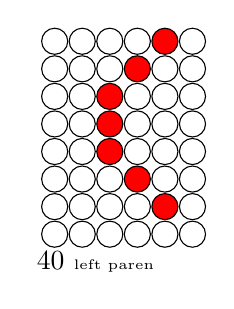
\begin{tikzpicture}[x=3.5mm,y=3.5mm]
\node [right] at (0,0) {40 {\tiny left paren}};
\node [circle, fill=none, draw=black, minimum size=3mm] at (1,8) {};
\node [circle, fill=none, draw=black, minimum size=3mm] at (2,8) {};
\node [circle, fill=none, draw=black, minimum size=3mm] at (3,8) {};
\node [circle, fill=none, draw=black, minimum size=3mm] at (4,8) {};
\node [circle, fill=red, draw=black, minimum size=3mm] at (5,8) {};
\node [circle, fill=none, draw=black, minimum size=3mm] at (6,8) {};
\node [circle, fill=none, draw=black, minimum size=3mm] at (1,7) {};
\node [circle, fill=none, draw=black, minimum size=3mm] at (2,7) {};
\node [circle, fill=none, draw=black, minimum size=3mm] at (3,7) {};
\node [circle, fill=red, draw=black, minimum size=3mm] at (4,7) {};
\node [circle, fill=none, draw=black, minimum size=3mm] at (5,7) {};
\node [circle, fill=none, draw=black, minimum size=3mm] at (6,7) {};
\node [circle, fill=none, draw=black, minimum size=3mm] at (1,6) {};
\node [circle, fill=none, draw=black, minimum size=3mm] at (2,6) {};
\node [circle, fill=red, draw=black, minimum size=3mm] at (3,6) {};
\node [circle, fill=none, draw=black, minimum size=3mm] at (4,6) {};
\node [circle, fill=none, draw=black, minimum size=3mm] at (5,6) {};
\node [circle, fill=none, draw=black, minimum size=3mm] at (6,6) {};
\node [circle, fill=none, draw=black, minimum size=3mm] at (1,5) {};
\node [circle, fill=none, draw=black, minimum size=3mm] at (2,5) {};
\node [circle, fill=red, draw=black, minimum size=3mm] at (3,5) {};
\node [circle, fill=none, draw=black, minimum size=3mm] at (4,5) {};
\node [circle, fill=none, draw=black, minimum size=3mm] at (5,5) {};
\node [circle, fill=none, draw=black, minimum size=3mm] at (6,5) {};
\node [circle, fill=none, draw=black, minimum size=3mm] at (1,4) {};
\node [circle, fill=none, draw=black, minimum size=3mm] at (2,4) {};
\node [circle, fill=red, draw=black, minimum size=3mm] at (3,4) {};
\node [circle, fill=none, draw=black, minimum size=3mm] at (4,4) {};
\node [circle, fill=none, draw=black, minimum size=3mm] at (5,4) {};
\node [circle, fill=none, draw=black, minimum size=3mm] at (6,4) {};
\node [circle, fill=none, draw=black, minimum size=3mm] at (1,3) {};
\node [circle, fill=none, draw=black, minimum size=3mm] at (2,3) {};
\node [circle, fill=none, draw=black, minimum size=3mm] at (3,3) {};
\node [circle, fill=red, draw=black, minimum size=3mm] at (4,3) {};
\node [circle, fill=none, draw=black, minimum size=3mm] at (5,3) {};
\node [circle, fill=none, draw=black, minimum size=3mm] at (6,3) {};
\node [circle, fill=none, draw=black, minimum size=3mm] at (1,2) {};
\node [circle, fill=none, draw=black, minimum size=3mm] at (2,2) {};
\node [circle, fill=none, draw=black, minimum size=3mm] at (3,2) {};
\node [circle, fill=none, draw=black, minimum size=3mm] at (4,2) {};
\node [circle, fill=red, draw=black, minimum size=3mm] at (5,2) {};
\node [circle, fill=none, draw=black, minimum size=3mm] at (6,2) {};
\node [circle, fill=none, draw=black, minimum size=3mm] at (1,1) {};
\node [circle, fill=none, draw=black, minimum size=3mm] at (2,1) {};
\node [circle, fill=none, draw=black, minimum size=3mm] at (3,1) {};
\node [circle, fill=none, draw=black, minimum size=3mm] at (4,1) {};
\node [circle, fill=none, draw=black, minimum size=3mm] at (5,1) {};
\node [circle, fill=none, draw=black, minimum size=3mm] at (6,1) {};
\end{tikzpicture}% font 0 codepoint 41 name right paren space 6 width 3 offset 35
~ 
\noindent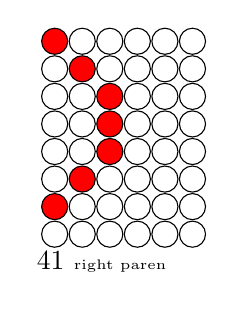
\begin{tikzpicture}[x=3.5mm,y=3.5mm]
\node [right] at (0,0) {41 {\tiny right paren}};
\node [circle, fill=red, draw=black, minimum size=3mm] at (1,8) {};
\node [circle, fill=none, draw=black, minimum size=3mm] at (2,8) {};
\node [circle, fill=none, draw=black, minimum size=3mm] at (3,8) {};
\node [circle, fill=none, draw=black, minimum size=3mm] at (4,8) {};
\node [circle, fill=none, draw=black, minimum size=3mm] at (5,8) {};
\node [circle, fill=none, draw=black, minimum size=3mm] at (6,8) {};
\node [circle, fill=none, draw=black, minimum size=3mm] at (1,7) {};
\node [circle, fill=red, draw=black, minimum size=3mm] at (2,7) {};
\node [circle, fill=none, draw=black, minimum size=3mm] at (3,7) {};
\node [circle, fill=none, draw=black, minimum size=3mm] at (4,7) {};
\node [circle, fill=none, draw=black, minimum size=3mm] at (5,7) {};
\node [circle, fill=none, draw=black, minimum size=3mm] at (6,7) {};
\node [circle, fill=none, draw=black, minimum size=3mm] at (1,6) {};
\node [circle, fill=none, draw=black, minimum size=3mm] at (2,6) {};
\node [circle, fill=red, draw=black, minimum size=3mm] at (3,6) {};
\node [circle, fill=none, draw=black, minimum size=3mm] at (4,6) {};
\node [circle, fill=none, draw=black, minimum size=3mm] at (5,6) {};
\node [circle, fill=none, draw=black, minimum size=3mm] at (6,6) {};
\node [circle, fill=none, draw=black, minimum size=3mm] at (1,5) {};
\node [circle, fill=none, draw=black, minimum size=3mm] at (2,5) {};
\node [circle, fill=red, draw=black, minimum size=3mm] at (3,5) {};
\node [circle, fill=none, draw=black, minimum size=3mm] at (4,5) {};
\node [circle, fill=none, draw=black, minimum size=3mm] at (5,5) {};
\node [circle, fill=none, draw=black, minimum size=3mm] at (6,5) {};
\node [circle, fill=none, draw=black, minimum size=3mm] at (1,4) {};
\node [circle, fill=none, draw=black, minimum size=3mm] at (2,4) {};
\node [circle, fill=red, draw=black, minimum size=3mm] at (3,4) {};
\node [circle, fill=none, draw=black, minimum size=3mm] at (4,4) {};
\node [circle, fill=none, draw=black, minimum size=3mm] at (5,4) {};
\node [circle, fill=none, draw=black, minimum size=3mm] at (6,4) {};
\node [circle, fill=none, draw=black, minimum size=3mm] at (1,3) {};
\node [circle, fill=red, draw=black, minimum size=3mm] at (2,3) {};
\node [circle, fill=none, draw=black, minimum size=3mm] at (3,3) {};
\node [circle, fill=none, draw=black, minimum size=3mm] at (4,3) {};
\node [circle, fill=none, draw=black, minimum size=3mm] at (5,3) {};
\node [circle, fill=none, draw=black, minimum size=3mm] at (6,3) {};
\node [circle, fill=red, draw=black, minimum size=3mm] at (1,2) {};
\node [circle, fill=none, draw=black, minimum size=3mm] at (2,2) {};
\node [circle, fill=none, draw=black, minimum size=3mm] at (3,2) {};
\node [circle, fill=none, draw=black, minimum size=3mm] at (4,2) {};
\node [circle, fill=none, draw=black, minimum size=3mm] at (5,2) {};
\node [circle, fill=none, draw=black, minimum size=3mm] at (6,2) {};
\node [circle, fill=none, draw=black, minimum size=3mm] at (1,1) {};
\node [circle, fill=none, draw=black, minimum size=3mm] at (2,1) {};
\node [circle, fill=none, draw=black, minimum size=3mm] at (3,1) {};
\node [circle, fill=none, draw=black, minimum size=3mm] at (4,1) {};
\node [circle, fill=none, draw=black, minimum size=3mm] at (5,1) {};
\node [circle, fill=none, draw=black, minimum size=3mm] at (6,1) {};
\end{tikzpicture}% font 0 codepoint 42 name asterisk space 6 width 5 offset 43


\noindent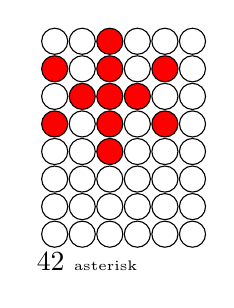
\begin{tikzpicture}[x=3.5mm,y=3.5mm]
\node [right] at (0,0) {42 {\tiny asterisk}};
\node [circle, fill=none, draw=black, minimum size=3mm] at (1,8) {};
\node [circle, fill=none, draw=black, minimum size=3mm] at (2,8) {};
\node [circle, fill=red, draw=black, minimum size=3mm] at (3,8) {};
\node [circle, fill=none, draw=black, minimum size=3mm] at (4,8) {};
\node [circle, fill=none, draw=black, minimum size=3mm] at (5,8) {};
\node [circle, fill=none, draw=black, minimum size=3mm] at (6,8) {};
\node [circle, fill=red, draw=black, minimum size=3mm] at (1,7) {};
\node [circle, fill=none, draw=black, minimum size=3mm] at (2,7) {};
\node [circle, fill=red, draw=black, minimum size=3mm] at (3,7) {};
\node [circle, fill=none, draw=black, minimum size=3mm] at (4,7) {};
\node [circle, fill=red, draw=black, minimum size=3mm] at (5,7) {};
\node [circle, fill=none, draw=black, minimum size=3mm] at (6,7) {};
\node [circle, fill=none, draw=black, minimum size=3mm] at (1,6) {};
\node [circle, fill=red, draw=black, minimum size=3mm] at (2,6) {};
\node [circle, fill=red, draw=black, minimum size=3mm] at (3,6) {};
\node [circle, fill=red, draw=black, minimum size=3mm] at (4,6) {};
\node [circle, fill=none, draw=black, minimum size=3mm] at (5,6) {};
\node [circle, fill=none, draw=black, minimum size=3mm] at (6,6) {};
\node [circle, fill=red, draw=black, minimum size=3mm] at (1,5) {};
\node [circle, fill=none, draw=black, minimum size=3mm] at (2,5) {};
\node [circle, fill=red, draw=black, minimum size=3mm] at (3,5) {};
\node [circle, fill=none, draw=black, minimum size=3mm] at (4,5) {};
\node [circle, fill=red, draw=black, minimum size=3mm] at (5,5) {};
\node [circle, fill=none, draw=black, minimum size=3mm] at (6,5) {};
\node [circle, fill=none, draw=black, minimum size=3mm] at (1,4) {};
\node [circle, fill=none, draw=black, minimum size=3mm] at (2,4) {};
\node [circle, fill=red, draw=black, minimum size=3mm] at (3,4) {};
\node [circle, fill=none, draw=black, minimum size=3mm] at (4,4) {};
\node [circle, fill=none, draw=black, minimum size=3mm] at (5,4) {};
\node [circle, fill=none, draw=black, minimum size=3mm] at (6,4) {};
\node [circle, fill=none, draw=black, minimum size=3mm] at (1,3) {};
\node [circle, fill=none, draw=black, minimum size=3mm] at (2,3) {};
\node [circle, fill=none, draw=black, minimum size=3mm] at (3,3) {};
\node [circle, fill=none, draw=black, minimum size=3mm] at (4,3) {};
\node [circle, fill=none, draw=black, minimum size=3mm] at (5,3) {};
\node [circle, fill=none, draw=black, minimum size=3mm] at (6,3) {};
\node [circle, fill=none, draw=black, minimum size=3mm] at (1,2) {};
\node [circle, fill=none, draw=black, minimum size=3mm] at (2,2) {};
\node [circle, fill=none, draw=black, minimum size=3mm] at (3,2) {};
\node [circle, fill=none, draw=black, minimum size=3mm] at (4,2) {};
\node [circle, fill=none, draw=black, minimum size=3mm] at (5,2) {};
\node [circle, fill=none, draw=black, minimum size=3mm] at (6,2) {};
\node [circle, fill=none, draw=black, minimum size=3mm] at (1,1) {};
\node [circle, fill=none, draw=black, minimum size=3mm] at (2,1) {};
\node [circle, fill=none, draw=black, minimum size=3mm] at (3,1) {};
\node [circle, fill=none, draw=black, minimum size=3mm] at (4,1) {};
\node [circle, fill=none, draw=black, minimum size=3mm] at (5,1) {};
\node [circle, fill=none, draw=black, minimum size=3mm] at (6,1) {};
\end{tikzpicture}% font 0 codepoint 43 name plus space 6 width 5 offset 48
~ 
\noindent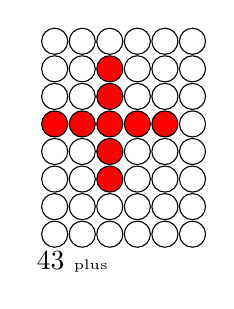
\begin{tikzpicture}[x=3.5mm,y=3.5mm]
\node [right] at (0,0) {43 {\tiny plus}};
\node [circle, fill=none, draw=black, minimum size=3mm] at (1,8) {};
\node [circle, fill=none, draw=black, minimum size=3mm] at (2,8) {};
\node [circle, fill=none, draw=black, minimum size=3mm] at (3,8) {};
\node [circle, fill=none, draw=black, minimum size=3mm] at (4,8) {};
\node [circle, fill=none, draw=black, minimum size=3mm] at (5,8) {};
\node [circle, fill=none, draw=black, minimum size=3mm] at (6,8) {};
\node [circle, fill=none, draw=black, minimum size=3mm] at (1,7) {};
\node [circle, fill=none, draw=black, minimum size=3mm] at (2,7) {};
\node [circle, fill=red, draw=black, minimum size=3mm] at (3,7) {};
\node [circle, fill=none, draw=black, minimum size=3mm] at (4,7) {};
\node [circle, fill=none, draw=black, minimum size=3mm] at (5,7) {};
\node [circle, fill=none, draw=black, minimum size=3mm] at (6,7) {};
\node [circle, fill=none, draw=black, minimum size=3mm] at (1,6) {};
\node [circle, fill=none, draw=black, minimum size=3mm] at (2,6) {};
\node [circle, fill=red, draw=black, minimum size=3mm] at (3,6) {};
\node [circle, fill=none, draw=black, minimum size=3mm] at (4,6) {};
\node [circle, fill=none, draw=black, minimum size=3mm] at (5,6) {};
\node [circle, fill=none, draw=black, minimum size=3mm] at (6,6) {};
\node [circle, fill=red, draw=black, minimum size=3mm] at (1,5) {};
\node [circle, fill=red, draw=black, minimum size=3mm] at (2,5) {};
\node [circle, fill=red, draw=black, minimum size=3mm] at (3,5) {};
\node [circle, fill=red, draw=black, minimum size=3mm] at (4,5) {};
\node [circle, fill=red, draw=black, minimum size=3mm] at (5,5) {};
\node [circle, fill=none, draw=black, minimum size=3mm] at (6,5) {};
\node [circle, fill=none, draw=black, minimum size=3mm] at (1,4) {};
\node [circle, fill=none, draw=black, minimum size=3mm] at (2,4) {};
\node [circle, fill=red, draw=black, minimum size=3mm] at (3,4) {};
\node [circle, fill=none, draw=black, minimum size=3mm] at (4,4) {};
\node [circle, fill=none, draw=black, minimum size=3mm] at (5,4) {};
\node [circle, fill=none, draw=black, minimum size=3mm] at (6,4) {};
\node [circle, fill=none, draw=black, minimum size=3mm] at (1,3) {};
\node [circle, fill=none, draw=black, minimum size=3mm] at (2,3) {};
\node [circle, fill=red, draw=black, minimum size=3mm] at (3,3) {};
\node [circle, fill=none, draw=black, minimum size=3mm] at (4,3) {};
\node [circle, fill=none, draw=black, minimum size=3mm] at (5,3) {};
\node [circle, fill=none, draw=black, minimum size=3mm] at (6,3) {};
\node [circle, fill=none, draw=black, minimum size=3mm] at (1,2) {};
\node [circle, fill=none, draw=black, minimum size=3mm] at (2,2) {};
\node [circle, fill=none, draw=black, minimum size=3mm] at (3,2) {};
\node [circle, fill=none, draw=black, minimum size=3mm] at (4,2) {};
\node [circle, fill=none, draw=black, minimum size=3mm] at (5,2) {};
\node [circle, fill=none, draw=black, minimum size=3mm] at (6,2) {};
\node [circle, fill=none, draw=black, minimum size=3mm] at (1,1) {};
\node [circle, fill=none, draw=black, minimum size=3mm] at (2,1) {};
\node [circle, fill=none, draw=black, minimum size=3mm] at (3,1) {};
\node [circle, fill=none, draw=black, minimum size=3mm] at (4,1) {};
\node [circle, fill=none, draw=black, minimum size=3mm] at (5,1) {};
\node [circle, fill=none, draw=black, minimum size=3mm] at (6,1) {};
\end{tikzpicture}% font 0 codepoint 44 name comma space 6 width 2 offset 53
~ 
\noindent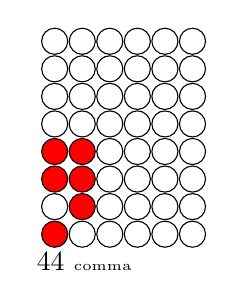
\begin{tikzpicture}[x=3.5mm,y=3.5mm]
\node [right] at (0,0) {44 {\tiny comma}};
\node [circle, fill=none, draw=black, minimum size=3mm] at (1,8) {};
\node [circle, fill=none, draw=black, minimum size=3mm] at (2,8) {};
\node [circle, fill=none, draw=black, minimum size=3mm] at (3,8) {};
\node [circle, fill=none, draw=black, minimum size=3mm] at (4,8) {};
\node [circle, fill=none, draw=black, minimum size=3mm] at (5,8) {};
\node [circle, fill=none, draw=black, minimum size=3mm] at (6,8) {};
\node [circle, fill=none, draw=black, minimum size=3mm] at (1,7) {};
\node [circle, fill=none, draw=black, minimum size=3mm] at (2,7) {};
\node [circle, fill=none, draw=black, minimum size=3mm] at (3,7) {};
\node [circle, fill=none, draw=black, minimum size=3mm] at (4,7) {};
\node [circle, fill=none, draw=black, minimum size=3mm] at (5,7) {};
\node [circle, fill=none, draw=black, minimum size=3mm] at (6,7) {};
\node [circle, fill=none, draw=black, minimum size=3mm] at (1,6) {};
\node [circle, fill=none, draw=black, minimum size=3mm] at (2,6) {};
\node [circle, fill=none, draw=black, minimum size=3mm] at (3,6) {};
\node [circle, fill=none, draw=black, minimum size=3mm] at (4,6) {};
\node [circle, fill=none, draw=black, minimum size=3mm] at (5,6) {};
\node [circle, fill=none, draw=black, minimum size=3mm] at (6,6) {};
\node [circle, fill=none, draw=black, minimum size=3mm] at (1,5) {};
\node [circle, fill=none, draw=black, minimum size=3mm] at (2,5) {};
\node [circle, fill=none, draw=black, minimum size=3mm] at (3,5) {};
\node [circle, fill=none, draw=black, minimum size=3mm] at (4,5) {};
\node [circle, fill=none, draw=black, minimum size=3mm] at (5,5) {};
\node [circle, fill=none, draw=black, minimum size=3mm] at (6,5) {};
\node [circle, fill=red, draw=black, minimum size=3mm] at (1,4) {};
\node [circle, fill=red, draw=black, minimum size=3mm] at (2,4) {};
\node [circle, fill=none, draw=black, minimum size=3mm] at (3,4) {};
\node [circle, fill=none, draw=black, minimum size=3mm] at (4,4) {};
\node [circle, fill=none, draw=black, minimum size=3mm] at (5,4) {};
\node [circle, fill=none, draw=black, minimum size=3mm] at (6,4) {};
\node [circle, fill=red, draw=black, minimum size=3mm] at (1,3) {};
\node [circle, fill=red, draw=black, minimum size=3mm] at (2,3) {};
\node [circle, fill=none, draw=black, minimum size=3mm] at (3,3) {};
\node [circle, fill=none, draw=black, minimum size=3mm] at (4,3) {};
\node [circle, fill=none, draw=black, minimum size=3mm] at (5,3) {};
\node [circle, fill=none, draw=black, minimum size=3mm] at (6,3) {};
\node [circle, fill=none, draw=black, minimum size=3mm] at (1,2) {};
\node [circle, fill=red, draw=black, minimum size=3mm] at (2,2) {};
\node [circle, fill=none, draw=black, minimum size=3mm] at (3,2) {};
\node [circle, fill=none, draw=black, minimum size=3mm] at (4,2) {};
\node [circle, fill=none, draw=black, minimum size=3mm] at (5,2) {};
\node [circle, fill=none, draw=black, minimum size=3mm] at (6,2) {};
\node [circle, fill=red, draw=black, minimum size=3mm] at (1,1) {};
\node [circle, fill=none, draw=black, minimum size=3mm] at (2,1) {};
\node [circle, fill=none, draw=black, minimum size=3mm] at (3,1) {};
\node [circle, fill=none, draw=black, minimum size=3mm] at (4,1) {};
\node [circle, fill=none, draw=black, minimum size=3mm] at (5,1) {};
\node [circle, fill=none, draw=black, minimum size=3mm] at (6,1) {};
\end{tikzpicture}% font 0 codepoint 45 name minus space 6 width 5 offset 55
~ 
\noindent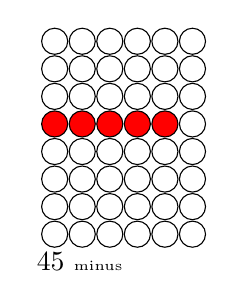
\begin{tikzpicture}[x=3.5mm,y=3.5mm]
\node [right] at (0,0) {45 {\tiny minus}};
\node [circle, fill=none, draw=black, minimum size=3mm] at (1,8) {};
\node [circle, fill=none, draw=black, minimum size=3mm] at (2,8) {};
\node [circle, fill=none, draw=black, minimum size=3mm] at (3,8) {};
\node [circle, fill=none, draw=black, minimum size=3mm] at (4,8) {};
\node [circle, fill=none, draw=black, minimum size=3mm] at (5,8) {};
\node [circle, fill=none, draw=black, minimum size=3mm] at (6,8) {};
\node [circle, fill=none, draw=black, minimum size=3mm] at (1,7) {};
\node [circle, fill=none, draw=black, minimum size=3mm] at (2,7) {};
\node [circle, fill=none, draw=black, minimum size=3mm] at (3,7) {};
\node [circle, fill=none, draw=black, minimum size=3mm] at (4,7) {};
\node [circle, fill=none, draw=black, minimum size=3mm] at (5,7) {};
\node [circle, fill=none, draw=black, minimum size=3mm] at (6,7) {};
\node [circle, fill=none, draw=black, minimum size=3mm] at (1,6) {};
\node [circle, fill=none, draw=black, minimum size=3mm] at (2,6) {};
\node [circle, fill=none, draw=black, minimum size=3mm] at (3,6) {};
\node [circle, fill=none, draw=black, minimum size=3mm] at (4,6) {};
\node [circle, fill=none, draw=black, minimum size=3mm] at (5,6) {};
\node [circle, fill=none, draw=black, minimum size=3mm] at (6,6) {};
\node [circle, fill=red, draw=black, minimum size=3mm] at (1,5) {};
\node [circle, fill=red, draw=black, minimum size=3mm] at (2,5) {};
\node [circle, fill=red, draw=black, minimum size=3mm] at (3,5) {};
\node [circle, fill=red, draw=black, minimum size=3mm] at (4,5) {};
\node [circle, fill=red, draw=black, minimum size=3mm] at (5,5) {};
\node [circle, fill=none, draw=black, minimum size=3mm] at (6,5) {};
\node [circle, fill=none, draw=black, minimum size=3mm] at (1,4) {};
\node [circle, fill=none, draw=black, minimum size=3mm] at (2,4) {};
\node [circle, fill=none, draw=black, minimum size=3mm] at (3,4) {};
\node [circle, fill=none, draw=black, minimum size=3mm] at (4,4) {};
\node [circle, fill=none, draw=black, minimum size=3mm] at (5,4) {};
\node [circle, fill=none, draw=black, minimum size=3mm] at (6,4) {};
\node [circle, fill=none, draw=black, minimum size=3mm] at (1,3) {};
\node [circle, fill=none, draw=black, minimum size=3mm] at (2,3) {};
\node [circle, fill=none, draw=black, minimum size=3mm] at (3,3) {};
\node [circle, fill=none, draw=black, minimum size=3mm] at (4,3) {};
\node [circle, fill=none, draw=black, minimum size=3mm] at (5,3) {};
\node [circle, fill=none, draw=black, minimum size=3mm] at (6,3) {};
\node [circle, fill=none, draw=black, minimum size=3mm] at (1,2) {};
\node [circle, fill=none, draw=black, minimum size=3mm] at (2,2) {};
\node [circle, fill=none, draw=black, minimum size=3mm] at (3,2) {};
\node [circle, fill=none, draw=black, minimum size=3mm] at (4,2) {};
\node [circle, fill=none, draw=black, minimum size=3mm] at (5,2) {};
\node [circle, fill=none, draw=black, minimum size=3mm] at (6,2) {};
\node [circle, fill=none, draw=black, minimum size=3mm] at (1,1) {};
\node [circle, fill=none, draw=black, minimum size=3mm] at (2,1) {};
\node [circle, fill=none, draw=black, minimum size=3mm] at (3,1) {};
\node [circle, fill=none, draw=black, minimum size=3mm] at (4,1) {};
\node [circle, fill=none, draw=black, minimum size=3mm] at (5,1) {};
\node [circle, fill=none, draw=black, minimum size=3mm] at (6,1) {};
\end{tikzpicture}% font 0 codepoint 46 name period space 6 width 2 offset 60
~ 
\noindent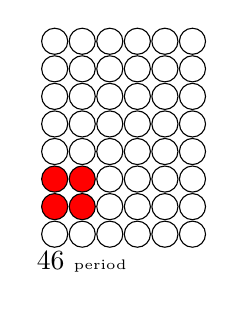
\begin{tikzpicture}[x=3.5mm,y=3.5mm]
\node [right] at (0,0) {46 {\tiny period}};
\node [circle, fill=none, draw=black, minimum size=3mm] at (1,8) {};
\node [circle, fill=none, draw=black, minimum size=3mm] at (2,8) {};
\node [circle, fill=none, draw=black, minimum size=3mm] at (3,8) {};
\node [circle, fill=none, draw=black, minimum size=3mm] at (4,8) {};
\node [circle, fill=none, draw=black, minimum size=3mm] at (5,8) {};
\node [circle, fill=none, draw=black, minimum size=3mm] at (6,8) {};
\node [circle, fill=none, draw=black, minimum size=3mm] at (1,7) {};
\node [circle, fill=none, draw=black, minimum size=3mm] at (2,7) {};
\node [circle, fill=none, draw=black, minimum size=3mm] at (3,7) {};
\node [circle, fill=none, draw=black, minimum size=3mm] at (4,7) {};
\node [circle, fill=none, draw=black, minimum size=3mm] at (5,7) {};
\node [circle, fill=none, draw=black, minimum size=3mm] at (6,7) {};
\node [circle, fill=none, draw=black, minimum size=3mm] at (1,6) {};
\node [circle, fill=none, draw=black, minimum size=3mm] at (2,6) {};
\node [circle, fill=none, draw=black, minimum size=3mm] at (3,6) {};
\node [circle, fill=none, draw=black, minimum size=3mm] at (4,6) {};
\node [circle, fill=none, draw=black, minimum size=3mm] at (5,6) {};
\node [circle, fill=none, draw=black, minimum size=3mm] at (6,6) {};
\node [circle, fill=none, draw=black, minimum size=3mm] at (1,5) {};
\node [circle, fill=none, draw=black, minimum size=3mm] at (2,5) {};
\node [circle, fill=none, draw=black, minimum size=3mm] at (3,5) {};
\node [circle, fill=none, draw=black, minimum size=3mm] at (4,5) {};
\node [circle, fill=none, draw=black, minimum size=3mm] at (5,5) {};
\node [circle, fill=none, draw=black, minimum size=3mm] at (6,5) {};
\node [circle, fill=none, draw=black, minimum size=3mm] at (1,4) {};
\node [circle, fill=none, draw=black, minimum size=3mm] at (2,4) {};
\node [circle, fill=none, draw=black, minimum size=3mm] at (3,4) {};
\node [circle, fill=none, draw=black, minimum size=3mm] at (4,4) {};
\node [circle, fill=none, draw=black, minimum size=3mm] at (5,4) {};
\node [circle, fill=none, draw=black, minimum size=3mm] at (6,4) {};
\node [circle, fill=red, draw=black, minimum size=3mm] at (1,3) {};
\node [circle, fill=red, draw=black, minimum size=3mm] at (2,3) {};
\node [circle, fill=none, draw=black, minimum size=3mm] at (3,3) {};
\node [circle, fill=none, draw=black, minimum size=3mm] at (4,3) {};
\node [circle, fill=none, draw=black, minimum size=3mm] at (5,3) {};
\node [circle, fill=none, draw=black, minimum size=3mm] at (6,3) {};
\node [circle, fill=red, draw=black, minimum size=3mm] at (1,2) {};
\node [circle, fill=red, draw=black, minimum size=3mm] at (2,2) {};
\node [circle, fill=none, draw=black, minimum size=3mm] at (3,2) {};
\node [circle, fill=none, draw=black, minimum size=3mm] at (4,2) {};
\node [circle, fill=none, draw=black, minimum size=3mm] at (5,2) {};
\node [circle, fill=none, draw=black, minimum size=3mm] at (6,2) {};
\node [circle, fill=none, draw=black, minimum size=3mm] at (1,1) {};
\node [circle, fill=none, draw=black, minimum size=3mm] at (2,1) {};
\node [circle, fill=none, draw=black, minimum size=3mm] at (3,1) {};
\node [circle, fill=none, draw=black, minimum size=3mm] at (4,1) {};
\node [circle, fill=none, draw=black, minimum size=3mm] at (5,1) {};
\node [circle, fill=none, draw=black, minimum size=3mm] at (6,1) {};
\end{tikzpicture}% font 0 codepoint 47 name slash space 6 width 5 offset 62


\noindent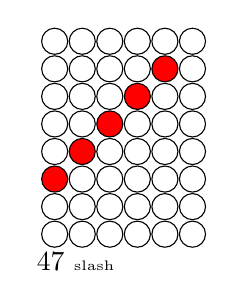
\begin{tikzpicture}[x=3.5mm,y=3.5mm]
\node [right] at (0,0) {47 {\tiny slash}};
\node [circle, fill=none, draw=black, minimum size=3mm] at (1,8) {};
\node [circle, fill=none, draw=black, minimum size=3mm] at (2,8) {};
\node [circle, fill=none, draw=black, minimum size=3mm] at (3,8) {};
\node [circle, fill=none, draw=black, minimum size=3mm] at (4,8) {};
\node [circle, fill=none, draw=black, minimum size=3mm] at (5,8) {};
\node [circle, fill=none, draw=black, minimum size=3mm] at (6,8) {};
\node [circle, fill=none, draw=black, minimum size=3mm] at (1,7) {};
\node [circle, fill=none, draw=black, minimum size=3mm] at (2,7) {};
\node [circle, fill=none, draw=black, minimum size=3mm] at (3,7) {};
\node [circle, fill=none, draw=black, minimum size=3mm] at (4,7) {};
\node [circle, fill=red, draw=black, minimum size=3mm] at (5,7) {};
\node [circle, fill=none, draw=black, minimum size=3mm] at (6,7) {};
\node [circle, fill=none, draw=black, minimum size=3mm] at (1,6) {};
\node [circle, fill=none, draw=black, minimum size=3mm] at (2,6) {};
\node [circle, fill=none, draw=black, minimum size=3mm] at (3,6) {};
\node [circle, fill=red, draw=black, minimum size=3mm] at (4,6) {};
\node [circle, fill=none, draw=black, minimum size=3mm] at (5,6) {};
\node [circle, fill=none, draw=black, minimum size=3mm] at (6,6) {};
\node [circle, fill=none, draw=black, minimum size=3mm] at (1,5) {};
\node [circle, fill=none, draw=black, minimum size=3mm] at (2,5) {};
\node [circle, fill=red, draw=black, minimum size=3mm] at (3,5) {};
\node [circle, fill=none, draw=black, minimum size=3mm] at (4,5) {};
\node [circle, fill=none, draw=black, minimum size=3mm] at (5,5) {};
\node [circle, fill=none, draw=black, minimum size=3mm] at (6,5) {};
\node [circle, fill=none, draw=black, minimum size=3mm] at (1,4) {};
\node [circle, fill=red, draw=black, minimum size=3mm] at (2,4) {};
\node [circle, fill=none, draw=black, minimum size=3mm] at (3,4) {};
\node [circle, fill=none, draw=black, minimum size=3mm] at (4,4) {};
\node [circle, fill=none, draw=black, minimum size=3mm] at (5,4) {};
\node [circle, fill=none, draw=black, minimum size=3mm] at (6,4) {};
\node [circle, fill=red, draw=black, minimum size=3mm] at (1,3) {};
\node [circle, fill=none, draw=black, minimum size=3mm] at (2,3) {};
\node [circle, fill=none, draw=black, minimum size=3mm] at (3,3) {};
\node [circle, fill=none, draw=black, minimum size=3mm] at (4,3) {};
\node [circle, fill=none, draw=black, minimum size=3mm] at (5,3) {};
\node [circle, fill=none, draw=black, minimum size=3mm] at (6,3) {};
\node [circle, fill=none, draw=black, minimum size=3mm] at (1,2) {};
\node [circle, fill=none, draw=black, minimum size=3mm] at (2,2) {};
\node [circle, fill=none, draw=black, minimum size=3mm] at (3,2) {};
\node [circle, fill=none, draw=black, minimum size=3mm] at (4,2) {};
\node [circle, fill=none, draw=black, minimum size=3mm] at (5,2) {};
\node [circle, fill=none, draw=black, minimum size=3mm] at (6,2) {};
\node [circle, fill=none, draw=black, minimum size=3mm] at (1,1) {};
\node [circle, fill=none, draw=black, minimum size=3mm] at (2,1) {};
\node [circle, fill=none, draw=black, minimum size=3mm] at (3,1) {};
\node [circle, fill=none, draw=black, minimum size=3mm] at (4,1) {};
\node [circle, fill=none, draw=black, minimum size=3mm] at (5,1) {};
\node [circle, fill=none, draw=black, minimum size=3mm] at (6,1) {};
\end{tikzpicture}% font 0 codepoint 48 name digit 0 space 6 width 5 offset 67
~ 
\noindent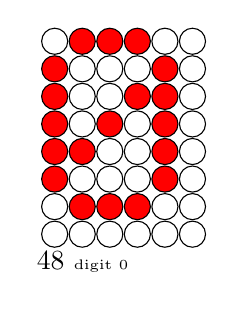
\begin{tikzpicture}[x=3.5mm,y=3.5mm]
\node [right] at (0,0) {48 {\tiny digit 0}};
\node [circle, fill=none, draw=black, minimum size=3mm] at (1,8) {};
\node [circle, fill=red, draw=black, minimum size=3mm] at (2,8) {};
\node [circle, fill=red, draw=black, minimum size=3mm] at (3,8) {};
\node [circle, fill=red, draw=black, minimum size=3mm] at (4,8) {};
\node [circle, fill=none, draw=black, minimum size=3mm] at (5,8) {};
\node [circle, fill=none, draw=black, minimum size=3mm] at (6,8) {};
\node [circle, fill=red, draw=black, minimum size=3mm] at (1,7) {};
\node [circle, fill=none, draw=black, minimum size=3mm] at (2,7) {};
\node [circle, fill=none, draw=black, minimum size=3mm] at (3,7) {};
\node [circle, fill=none, draw=black, minimum size=3mm] at (4,7) {};
\node [circle, fill=red, draw=black, minimum size=3mm] at (5,7) {};
\node [circle, fill=none, draw=black, minimum size=3mm] at (6,7) {};
\node [circle, fill=red, draw=black, minimum size=3mm] at (1,6) {};
\node [circle, fill=none, draw=black, minimum size=3mm] at (2,6) {};
\node [circle, fill=none, draw=black, minimum size=3mm] at (3,6) {};
\node [circle, fill=red, draw=black, minimum size=3mm] at (4,6) {};
\node [circle, fill=red, draw=black, minimum size=3mm] at (5,6) {};
\node [circle, fill=none, draw=black, minimum size=3mm] at (6,6) {};
\node [circle, fill=red, draw=black, minimum size=3mm] at (1,5) {};
\node [circle, fill=none, draw=black, minimum size=3mm] at (2,5) {};
\node [circle, fill=red, draw=black, minimum size=3mm] at (3,5) {};
\node [circle, fill=none, draw=black, minimum size=3mm] at (4,5) {};
\node [circle, fill=red, draw=black, minimum size=3mm] at (5,5) {};
\node [circle, fill=none, draw=black, minimum size=3mm] at (6,5) {};
\node [circle, fill=red, draw=black, minimum size=3mm] at (1,4) {};
\node [circle, fill=red, draw=black, minimum size=3mm] at (2,4) {};
\node [circle, fill=none, draw=black, minimum size=3mm] at (3,4) {};
\node [circle, fill=none, draw=black, minimum size=3mm] at (4,4) {};
\node [circle, fill=red, draw=black, minimum size=3mm] at (5,4) {};
\node [circle, fill=none, draw=black, minimum size=3mm] at (6,4) {};
\node [circle, fill=red, draw=black, minimum size=3mm] at (1,3) {};
\node [circle, fill=none, draw=black, minimum size=3mm] at (2,3) {};
\node [circle, fill=none, draw=black, minimum size=3mm] at (3,3) {};
\node [circle, fill=none, draw=black, minimum size=3mm] at (4,3) {};
\node [circle, fill=red, draw=black, minimum size=3mm] at (5,3) {};
\node [circle, fill=none, draw=black, minimum size=3mm] at (6,3) {};
\node [circle, fill=none, draw=black, minimum size=3mm] at (1,2) {};
\node [circle, fill=red, draw=black, minimum size=3mm] at (2,2) {};
\node [circle, fill=red, draw=black, minimum size=3mm] at (3,2) {};
\node [circle, fill=red, draw=black, minimum size=3mm] at (4,2) {};
\node [circle, fill=none, draw=black, minimum size=3mm] at (5,2) {};
\node [circle, fill=none, draw=black, minimum size=3mm] at (6,2) {};
\node [circle, fill=none, draw=black, minimum size=3mm] at (1,1) {};
\node [circle, fill=none, draw=black, minimum size=3mm] at (2,1) {};
\node [circle, fill=none, draw=black, minimum size=3mm] at (3,1) {};
\node [circle, fill=none, draw=black, minimum size=3mm] at (4,1) {};
\node [circle, fill=none, draw=black, minimum size=3mm] at (5,1) {};
\node [circle, fill=none, draw=black, minimum size=3mm] at (6,1) {};
\end{tikzpicture}% font 0 codepoint 49 name digit 1 space 6 width 5 offset 72
~ 
\noindent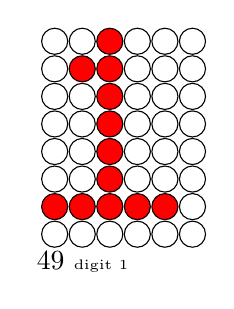
\begin{tikzpicture}[x=3.5mm,y=3.5mm]
\node [right] at (0,0) {49 {\tiny digit 1}};
\node [circle, fill=none, draw=black, minimum size=3mm] at (1,8) {};
\node [circle, fill=none, draw=black, minimum size=3mm] at (2,8) {};
\node [circle, fill=red, draw=black, minimum size=3mm] at (3,8) {};
\node [circle, fill=none, draw=black, minimum size=3mm] at (4,8) {};
\node [circle, fill=none, draw=black, minimum size=3mm] at (5,8) {};
\node [circle, fill=none, draw=black, minimum size=3mm] at (6,8) {};
\node [circle, fill=none, draw=black, minimum size=3mm] at (1,7) {};
\node [circle, fill=red, draw=black, minimum size=3mm] at (2,7) {};
\node [circle, fill=red, draw=black, minimum size=3mm] at (3,7) {};
\node [circle, fill=none, draw=black, minimum size=3mm] at (4,7) {};
\node [circle, fill=none, draw=black, minimum size=3mm] at (5,7) {};
\node [circle, fill=none, draw=black, minimum size=3mm] at (6,7) {};
\node [circle, fill=none, draw=black, minimum size=3mm] at (1,6) {};
\node [circle, fill=none, draw=black, minimum size=3mm] at (2,6) {};
\node [circle, fill=red, draw=black, minimum size=3mm] at (3,6) {};
\node [circle, fill=none, draw=black, minimum size=3mm] at (4,6) {};
\node [circle, fill=none, draw=black, minimum size=3mm] at (5,6) {};
\node [circle, fill=none, draw=black, minimum size=3mm] at (6,6) {};
\node [circle, fill=none, draw=black, minimum size=3mm] at (1,5) {};
\node [circle, fill=none, draw=black, minimum size=3mm] at (2,5) {};
\node [circle, fill=red, draw=black, minimum size=3mm] at (3,5) {};
\node [circle, fill=none, draw=black, minimum size=3mm] at (4,5) {};
\node [circle, fill=none, draw=black, minimum size=3mm] at (5,5) {};
\node [circle, fill=none, draw=black, minimum size=3mm] at (6,5) {};
\node [circle, fill=none, draw=black, minimum size=3mm] at (1,4) {};
\node [circle, fill=none, draw=black, minimum size=3mm] at (2,4) {};
\node [circle, fill=red, draw=black, minimum size=3mm] at (3,4) {};
\node [circle, fill=none, draw=black, minimum size=3mm] at (4,4) {};
\node [circle, fill=none, draw=black, minimum size=3mm] at (5,4) {};
\node [circle, fill=none, draw=black, minimum size=3mm] at (6,4) {};
\node [circle, fill=none, draw=black, minimum size=3mm] at (1,3) {};
\node [circle, fill=none, draw=black, minimum size=3mm] at (2,3) {};
\node [circle, fill=red, draw=black, minimum size=3mm] at (3,3) {};
\node [circle, fill=none, draw=black, minimum size=3mm] at (4,3) {};
\node [circle, fill=none, draw=black, minimum size=3mm] at (5,3) {};
\node [circle, fill=none, draw=black, minimum size=3mm] at (6,3) {};
\node [circle, fill=red, draw=black, minimum size=3mm] at (1,2) {};
\node [circle, fill=red, draw=black, minimum size=3mm] at (2,2) {};
\node [circle, fill=red, draw=black, minimum size=3mm] at (3,2) {};
\node [circle, fill=red, draw=black, minimum size=3mm] at (4,2) {};
\node [circle, fill=red, draw=black, minimum size=3mm] at (5,2) {};
\node [circle, fill=none, draw=black, minimum size=3mm] at (6,2) {};
\node [circle, fill=none, draw=black, minimum size=3mm] at (1,1) {};
\node [circle, fill=none, draw=black, minimum size=3mm] at (2,1) {};
\node [circle, fill=none, draw=black, minimum size=3mm] at (3,1) {};
\node [circle, fill=none, draw=black, minimum size=3mm] at (4,1) {};
\node [circle, fill=none, draw=black, minimum size=3mm] at (5,1) {};
\node [circle, fill=none, draw=black, minimum size=3mm] at (6,1) {};
\end{tikzpicture}% font 0 codepoint 50 name digit 2 space 6 width 5 offset 77
~ 
\noindent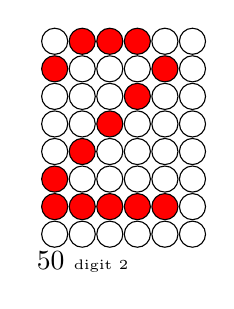
\begin{tikzpicture}[x=3.5mm,y=3.5mm]
\node [right] at (0,0) {50 {\tiny digit 2}};
\node [circle, fill=none, draw=black, minimum size=3mm] at (1,8) {};
\node [circle, fill=red, draw=black, minimum size=3mm] at (2,8) {};
\node [circle, fill=red, draw=black, minimum size=3mm] at (3,8) {};
\node [circle, fill=red, draw=black, minimum size=3mm] at (4,8) {};
\node [circle, fill=none, draw=black, minimum size=3mm] at (5,8) {};
\node [circle, fill=none, draw=black, minimum size=3mm] at (6,8) {};
\node [circle, fill=red, draw=black, minimum size=3mm] at (1,7) {};
\node [circle, fill=none, draw=black, minimum size=3mm] at (2,7) {};
\node [circle, fill=none, draw=black, minimum size=3mm] at (3,7) {};
\node [circle, fill=none, draw=black, minimum size=3mm] at (4,7) {};
\node [circle, fill=red, draw=black, minimum size=3mm] at (5,7) {};
\node [circle, fill=none, draw=black, minimum size=3mm] at (6,7) {};
\node [circle, fill=none, draw=black, minimum size=3mm] at (1,6) {};
\node [circle, fill=none, draw=black, minimum size=3mm] at (2,6) {};
\node [circle, fill=none, draw=black, minimum size=3mm] at (3,6) {};
\node [circle, fill=red, draw=black, minimum size=3mm] at (4,6) {};
\node [circle, fill=none, draw=black, minimum size=3mm] at (5,6) {};
\node [circle, fill=none, draw=black, minimum size=3mm] at (6,6) {};
\node [circle, fill=none, draw=black, minimum size=3mm] at (1,5) {};
\node [circle, fill=none, draw=black, minimum size=3mm] at (2,5) {};
\node [circle, fill=red, draw=black, minimum size=3mm] at (3,5) {};
\node [circle, fill=none, draw=black, minimum size=3mm] at (4,5) {};
\node [circle, fill=none, draw=black, minimum size=3mm] at (5,5) {};
\node [circle, fill=none, draw=black, minimum size=3mm] at (6,5) {};
\node [circle, fill=none, draw=black, minimum size=3mm] at (1,4) {};
\node [circle, fill=red, draw=black, minimum size=3mm] at (2,4) {};
\node [circle, fill=none, draw=black, minimum size=3mm] at (3,4) {};
\node [circle, fill=none, draw=black, minimum size=3mm] at (4,4) {};
\node [circle, fill=none, draw=black, minimum size=3mm] at (5,4) {};
\node [circle, fill=none, draw=black, minimum size=3mm] at (6,4) {};
\node [circle, fill=red, draw=black, minimum size=3mm] at (1,3) {};
\node [circle, fill=none, draw=black, minimum size=3mm] at (2,3) {};
\node [circle, fill=none, draw=black, minimum size=3mm] at (3,3) {};
\node [circle, fill=none, draw=black, minimum size=3mm] at (4,3) {};
\node [circle, fill=none, draw=black, minimum size=3mm] at (5,3) {};
\node [circle, fill=none, draw=black, minimum size=3mm] at (6,3) {};
\node [circle, fill=red, draw=black, minimum size=3mm] at (1,2) {};
\node [circle, fill=red, draw=black, minimum size=3mm] at (2,2) {};
\node [circle, fill=red, draw=black, minimum size=3mm] at (3,2) {};
\node [circle, fill=red, draw=black, minimum size=3mm] at (4,2) {};
\node [circle, fill=red, draw=black, minimum size=3mm] at (5,2) {};
\node [circle, fill=none, draw=black, minimum size=3mm] at (6,2) {};
\node [circle, fill=none, draw=black, minimum size=3mm] at (1,1) {};
\node [circle, fill=none, draw=black, minimum size=3mm] at (2,1) {};
\node [circle, fill=none, draw=black, minimum size=3mm] at (3,1) {};
\node [circle, fill=none, draw=black, minimum size=3mm] at (4,1) {};
\node [circle, fill=none, draw=black, minimum size=3mm] at (5,1) {};
\node [circle, fill=none, draw=black, minimum size=3mm] at (6,1) {};
\end{tikzpicture}% font 0 codepoint 51 name digit 3 space 6 width 5 offset 82
~ 
\noindent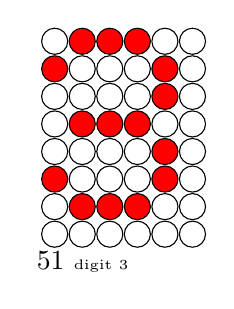
\begin{tikzpicture}[x=3.5mm,y=3.5mm]
\node [right] at (0,0) {51 {\tiny digit 3}};
\node [circle, fill=none, draw=black, minimum size=3mm] at (1,8) {};
\node [circle, fill=red, draw=black, minimum size=3mm] at (2,8) {};
\node [circle, fill=red, draw=black, minimum size=3mm] at (3,8) {};
\node [circle, fill=red, draw=black, minimum size=3mm] at (4,8) {};
\node [circle, fill=none, draw=black, minimum size=3mm] at (5,8) {};
\node [circle, fill=none, draw=black, minimum size=3mm] at (6,8) {};
\node [circle, fill=red, draw=black, minimum size=3mm] at (1,7) {};
\node [circle, fill=none, draw=black, minimum size=3mm] at (2,7) {};
\node [circle, fill=none, draw=black, minimum size=3mm] at (3,7) {};
\node [circle, fill=none, draw=black, minimum size=3mm] at (4,7) {};
\node [circle, fill=red, draw=black, minimum size=3mm] at (5,7) {};
\node [circle, fill=none, draw=black, minimum size=3mm] at (6,7) {};
\node [circle, fill=none, draw=black, minimum size=3mm] at (1,6) {};
\node [circle, fill=none, draw=black, minimum size=3mm] at (2,6) {};
\node [circle, fill=none, draw=black, minimum size=3mm] at (3,6) {};
\node [circle, fill=none, draw=black, minimum size=3mm] at (4,6) {};
\node [circle, fill=red, draw=black, minimum size=3mm] at (5,6) {};
\node [circle, fill=none, draw=black, minimum size=3mm] at (6,6) {};
\node [circle, fill=none, draw=black, minimum size=3mm] at (1,5) {};
\node [circle, fill=red, draw=black, minimum size=3mm] at (2,5) {};
\node [circle, fill=red, draw=black, minimum size=3mm] at (3,5) {};
\node [circle, fill=red, draw=black, minimum size=3mm] at (4,5) {};
\node [circle, fill=none, draw=black, minimum size=3mm] at (5,5) {};
\node [circle, fill=none, draw=black, minimum size=3mm] at (6,5) {};
\node [circle, fill=none, draw=black, minimum size=3mm] at (1,4) {};
\node [circle, fill=none, draw=black, minimum size=3mm] at (2,4) {};
\node [circle, fill=none, draw=black, minimum size=3mm] at (3,4) {};
\node [circle, fill=none, draw=black, minimum size=3mm] at (4,4) {};
\node [circle, fill=red, draw=black, minimum size=3mm] at (5,4) {};
\node [circle, fill=none, draw=black, minimum size=3mm] at (6,4) {};
\node [circle, fill=red, draw=black, minimum size=3mm] at (1,3) {};
\node [circle, fill=none, draw=black, minimum size=3mm] at (2,3) {};
\node [circle, fill=none, draw=black, minimum size=3mm] at (3,3) {};
\node [circle, fill=none, draw=black, minimum size=3mm] at (4,3) {};
\node [circle, fill=red, draw=black, minimum size=3mm] at (5,3) {};
\node [circle, fill=none, draw=black, minimum size=3mm] at (6,3) {};
\node [circle, fill=none, draw=black, minimum size=3mm] at (1,2) {};
\node [circle, fill=red, draw=black, minimum size=3mm] at (2,2) {};
\node [circle, fill=red, draw=black, minimum size=3mm] at (3,2) {};
\node [circle, fill=red, draw=black, minimum size=3mm] at (4,2) {};
\node [circle, fill=none, draw=black, minimum size=3mm] at (5,2) {};
\node [circle, fill=none, draw=black, minimum size=3mm] at (6,2) {};
\node [circle, fill=none, draw=black, minimum size=3mm] at (1,1) {};
\node [circle, fill=none, draw=black, minimum size=3mm] at (2,1) {};
\node [circle, fill=none, draw=black, minimum size=3mm] at (3,1) {};
\node [circle, fill=none, draw=black, minimum size=3mm] at (4,1) {};
\node [circle, fill=none, draw=black, minimum size=3mm] at (5,1) {};
\node [circle, fill=none, draw=black, minimum size=3mm] at (6,1) {};
\end{tikzpicture}% font 0 codepoint 52 name digit 4 space 6 width 5 offset 87


\noindent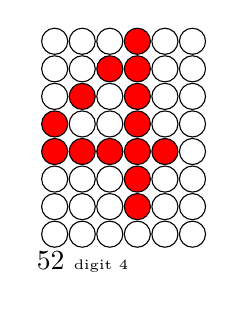
\begin{tikzpicture}[x=3.5mm,y=3.5mm]
\node [right] at (0,0) {52 {\tiny digit 4}};
\node [circle, fill=none, draw=black, minimum size=3mm] at (1,8) {};
\node [circle, fill=none, draw=black, minimum size=3mm] at (2,8) {};
\node [circle, fill=none, draw=black, minimum size=3mm] at (3,8) {};
\node [circle, fill=red, draw=black, minimum size=3mm] at (4,8) {};
\node [circle, fill=none, draw=black, minimum size=3mm] at (5,8) {};
\node [circle, fill=none, draw=black, minimum size=3mm] at (6,8) {};
\node [circle, fill=none, draw=black, minimum size=3mm] at (1,7) {};
\node [circle, fill=none, draw=black, minimum size=3mm] at (2,7) {};
\node [circle, fill=red, draw=black, minimum size=3mm] at (3,7) {};
\node [circle, fill=red, draw=black, minimum size=3mm] at (4,7) {};
\node [circle, fill=none, draw=black, minimum size=3mm] at (5,7) {};
\node [circle, fill=none, draw=black, minimum size=3mm] at (6,7) {};
\node [circle, fill=none, draw=black, minimum size=3mm] at (1,6) {};
\node [circle, fill=red, draw=black, minimum size=3mm] at (2,6) {};
\node [circle, fill=none, draw=black, minimum size=3mm] at (3,6) {};
\node [circle, fill=red, draw=black, minimum size=3mm] at (4,6) {};
\node [circle, fill=none, draw=black, minimum size=3mm] at (5,6) {};
\node [circle, fill=none, draw=black, minimum size=3mm] at (6,6) {};
\node [circle, fill=red, draw=black, minimum size=3mm] at (1,5) {};
\node [circle, fill=none, draw=black, minimum size=3mm] at (2,5) {};
\node [circle, fill=none, draw=black, minimum size=3mm] at (3,5) {};
\node [circle, fill=red, draw=black, minimum size=3mm] at (4,5) {};
\node [circle, fill=none, draw=black, minimum size=3mm] at (5,5) {};
\node [circle, fill=none, draw=black, minimum size=3mm] at (6,5) {};
\node [circle, fill=red, draw=black, minimum size=3mm] at (1,4) {};
\node [circle, fill=red, draw=black, minimum size=3mm] at (2,4) {};
\node [circle, fill=red, draw=black, minimum size=3mm] at (3,4) {};
\node [circle, fill=red, draw=black, minimum size=3mm] at (4,4) {};
\node [circle, fill=red, draw=black, minimum size=3mm] at (5,4) {};
\node [circle, fill=none, draw=black, minimum size=3mm] at (6,4) {};
\node [circle, fill=none, draw=black, minimum size=3mm] at (1,3) {};
\node [circle, fill=none, draw=black, minimum size=3mm] at (2,3) {};
\node [circle, fill=none, draw=black, minimum size=3mm] at (3,3) {};
\node [circle, fill=red, draw=black, minimum size=3mm] at (4,3) {};
\node [circle, fill=none, draw=black, minimum size=3mm] at (5,3) {};
\node [circle, fill=none, draw=black, minimum size=3mm] at (6,3) {};
\node [circle, fill=none, draw=black, minimum size=3mm] at (1,2) {};
\node [circle, fill=none, draw=black, minimum size=3mm] at (2,2) {};
\node [circle, fill=none, draw=black, minimum size=3mm] at (3,2) {};
\node [circle, fill=red, draw=black, minimum size=3mm] at (4,2) {};
\node [circle, fill=none, draw=black, minimum size=3mm] at (5,2) {};
\node [circle, fill=none, draw=black, minimum size=3mm] at (6,2) {};
\node [circle, fill=none, draw=black, minimum size=3mm] at (1,1) {};
\node [circle, fill=none, draw=black, minimum size=3mm] at (2,1) {};
\node [circle, fill=none, draw=black, minimum size=3mm] at (3,1) {};
\node [circle, fill=none, draw=black, minimum size=3mm] at (4,1) {};
\node [circle, fill=none, draw=black, minimum size=3mm] at (5,1) {};
\node [circle, fill=none, draw=black, minimum size=3mm] at (6,1) {};
\end{tikzpicture}% font 0 codepoint 53 name digit 5 space 6 width 5 offset 92
~ 
\noindent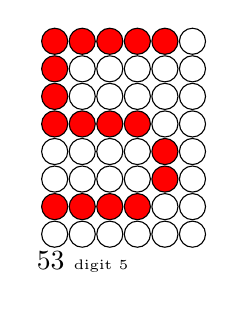
\begin{tikzpicture}[x=3.5mm,y=3.5mm]
\node [right] at (0,0) {53 {\tiny digit 5}};
\node [circle, fill=red, draw=black, minimum size=3mm] at (1,8) {};
\node [circle, fill=red, draw=black, minimum size=3mm] at (2,8) {};
\node [circle, fill=red, draw=black, minimum size=3mm] at (3,8) {};
\node [circle, fill=red, draw=black, minimum size=3mm] at (4,8) {};
\node [circle, fill=red, draw=black, minimum size=3mm] at (5,8) {};
\node [circle, fill=none, draw=black, minimum size=3mm] at (6,8) {};
\node [circle, fill=red, draw=black, minimum size=3mm] at (1,7) {};
\node [circle, fill=none, draw=black, minimum size=3mm] at (2,7) {};
\node [circle, fill=none, draw=black, minimum size=3mm] at (3,7) {};
\node [circle, fill=none, draw=black, minimum size=3mm] at (4,7) {};
\node [circle, fill=none, draw=black, minimum size=3mm] at (5,7) {};
\node [circle, fill=none, draw=black, minimum size=3mm] at (6,7) {};
\node [circle, fill=red, draw=black, minimum size=3mm] at (1,6) {};
\node [circle, fill=none, draw=black, minimum size=3mm] at (2,6) {};
\node [circle, fill=none, draw=black, minimum size=3mm] at (3,6) {};
\node [circle, fill=none, draw=black, minimum size=3mm] at (4,6) {};
\node [circle, fill=none, draw=black, minimum size=3mm] at (5,6) {};
\node [circle, fill=none, draw=black, minimum size=3mm] at (6,6) {};
\node [circle, fill=red, draw=black, minimum size=3mm] at (1,5) {};
\node [circle, fill=red, draw=black, minimum size=3mm] at (2,5) {};
\node [circle, fill=red, draw=black, minimum size=3mm] at (3,5) {};
\node [circle, fill=red, draw=black, minimum size=3mm] at (4,5) {};
\node [circle, fill=none, draw=black, minimum size=3mm] at (5,5) {};
\node [circle, fill=none, draw=black, minimum size=3mm] at (6,5) {};
\node [circle, fill=none, draw=black, minimum size=3mm] at (1,4) {};
\node [circle, fill=none, draw=black, minimum size=3mm] at (2,4) {};
\node [circle, fill=none, draw=black, minimum size=3mm] at (3,4) {};
\node [circle, fill=none, draw=black, minimum size=3mm] at (4,4) {};
\node [circle, fill=red, draw=black, minimum size=3mm] at (5,4) {};
\node [circle, fill=none, draw=black, minimum size=3mm] at (6,4) {};
\node [circle, fill=none, draw=black, minimum size=3mm] at (1,3) {};
\node [circle, fill=none, draw=black, minimum size=3mm] at (2,3) {};
\node [circle, fill=none, draw=black, minimum size=3mm] at (3,3) {};
\node [circle, fill=none, draw=black, minimum size=3mm] at (4,3) {};
\node [circle, fill=red, draw=black, minimum size=3mm] at (5,3) {};
\node [circle, fill=none, draw=black, minimum size=3mm] at (6,3) {};
\node [circle, fill=red, draw=black, minimum size=3mm] at (1,2) {};
\node [circle, fill=red, draw=black, minimum size=3mm] at (2,2) {};
\node [circle, fill=red, draw=black, minimum size=3mm] at (3,2) {};
\node [circle, fill=red, draw=black, minimum size=3mm] at (4,2) {};
\node [circle, fill=none, draw=black, minimum size=3mm] at (5,2) {};
\node [circle, fill=none, draw=black, minimum size=3mm] at (6,2) {};
\node [circle, fill=none, draw=black, minimum size=3mm] at (1,1) {};
\node [circle, fill=none, draw=black, minimum size=3mm] at (2,1) {};
\node [circle, fill=none, draw=black, minimum size=3mm] at (3,1) {};
\node [circle, fill=none, draw=black, minimum size=3mm] at (4,1) {};
\node [circle, fill=none, draw=black, minimum size=3mm] at (5,1) {};
\node [circle, fill=none, draw=black, minimum size=3mm] at (6,1) {};
\end{tikzpicture}% font 0 codepoint 54 name digit 6 space 6 width 5 offset 97
~ 
\noindent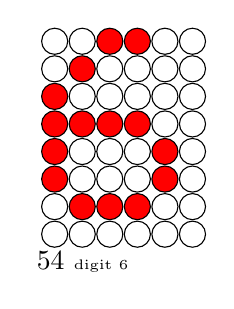
\begin{tikzpicture}[x=3.5mm,y=3.5mm]
\node [right] at (0,0) {54 {\tiny digit 6}};
\node [circle, fill=none, draw=black, minimum size=3mm] at (1,8) {};
\node [circle, fill=none, draw=black, minimum size=3mm] at (2,8) {};
\node [circle, fill=red, draw=black, minimum size=3mm] at (3,8) {};
\node [circle, fill=red, draw=black, minimum size=3mm] at (4,8) {};
\node [circle, fill=none, draw=black, minimum size=3mm] at (5,8) {};
\node [circle, fill=none, draw=black, minimum size=3mm] at (6,8) {};
\node [circle, fill=none, draw=black, minimum size=3mm] at (1,7) {};
\node [circle, fill=red, draw=black, minimum size=3mm] at (2,7) {};
\node [circle, fill=none, draw=black, minimum size=3mm] at (3,7) {};
\node [circle, fill=none, draw=black, minimum size=3mm] at (4,7) {};
\node [circle, fill=none, draw=black, minimum size=3mm] at (5,7) {};
\node [circle, fill=none, draw=black, minimum size=3mm] at (6,7) {};
\node [circle, fill=red, draw=black, minimum size=3mm] at (1,6) {};
\node [circle, fill=none, draw=black, minimum size=3mm] at (2,6) {};
\node [circle, fill=none, draw=black, minimum size=3mm] at (3,6) {};
\node [circle, fill=none, draw=black, minimum size=3mm] at (4,6) {};
\node [circle, fill=none, draw=black, minimum size=3mm] at (5,6) {};
\node [circle, fill=none, draw=black, minimum size=3mm] at (6,6) {};
\node [circle, fill=red, draw=black, minimum size=3mm] at (1,5) {};
\node [circle, fill=red, draw=black, minimum size=3mm] at (2,5) {};
\node [circle, fill=red, draw=black, minimum size=3mm] at (3,5) {};
\node [circle, fill=red, draw=black, minimum size=3mm] at (4,5) {};
\node [circle, fill=none, draw=black, minimum size=3mm] at (5,5) {};
\node [circle, fill=none, draw=black, minimum size=3mm] at (6,5) {};
\node [circle, fill=red, draw=black, minimum size=3mm] at (1,4) {};
\node [circle, fill=none, draw=black, minimum size=3mm] at (2,4) {};
\node [circle, fill=none, draw=black, minimum size=3mm] at (3,4) {};
\node [circle, fill=none, draw=black, minimum size=3mm] at (4,4) {};
\node [circle, fill=red, draw=black, minimum size=3mm] at (5,4) {};
\node [circle, fill=none, draw=black, minimum size=3mm] at (6,4) {};
\node [circle, fill=red, draw=black, minimum size=3mm] at (1,3) {};
\node [circle, fill=none, draw=black, minimum size=3mm] at (2,3) {};
\node [circle, fill=none, draw=black, minimum size=3mm] at (3,3) {};
\node [circle, fill=none, draw=black, minimum size=3mm] at (4,3) {};
\node [circle, fill=red, draw=black, minimum size=3mm] at (5,3) {};
\node [circle, fill=none, draw=black, minimum size=3mm] at (6,3) {};
\node [circle, fill=none, draw=black, minimum size=3mm] at (1,2) {};
\node [circle, fill=red, draw=black, minimum size=3mm] at (2,2) {};
\node [circle, fill=red, draw=black, minimum size=3mm] at (3,2) {};
\node [circle, fill=red, draw=black, minimum size=3mm] at (4,2) {};
\node [circle, fill=none, draw=black, minimum size=3mm] at (5,2) {};
\node [circle, fill=none, draw=black, minimum size=3mm] at (6,2) {};
\node [circle, fill=none, draw=black, minimum size=3mm] at (1,1) {};
\node [circle, fill=none, draw=black, minimum size=3mm] at (2,1) {};
\node [circle, fill=none, draw=black, minimum size=3mm] at (3,1) {};
\node [circle, fill=none, draw=black, minimum size=3mm] at (4,1) {};
\node [circle, fill=none, draw=black, minimum size=3mm] at (5,1) {};
\node [circle, fill=none, draw=black, minimum size=3mm] at (6,1) {};
\end{tikzpicture}% font 0 codepoint 55 name digit 7 space 6 width 5 offset 102
~ 
\noindent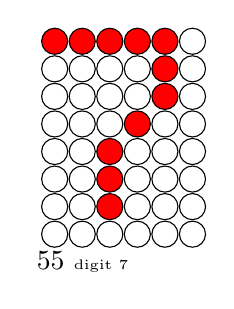
\begin{tikzpicture}[x=3.5mm,y=3.5mm]
\node [right] at (0,0) {55 {\tiny digit 7}};
\node [circle, fill=red, draw=black, minimum size=3mm] at (1,8) {};
\node [circle, fill=red, draw=black, minimum size=3mm] at (2,8) {};
\node [circle, fill=red, draw=black, minimum size=3mm] at (3,8) {};
\node [circle, fill=red, draw=black, minimum size=3mm] at (4,8) {};
\node [circle, fill=red, draw=black, minimum size=3mm] at (5,8) {};
\node [circle, fill=none, draw=black, minimum size=3mm] at (6,8) {};
\node [circle, fill=none, draw=black, minimum size=3mm] at (1,7) {};
\node [circle, fill=none, draw=black, minimum size=3mm] at (2,7) {};
\node [circle, fill=none, draw=black, minimum size=3mm] at (3,7) {};
\node [circle, fill=none, draw=black, minimum size=3mm] at (4,7) {};
\node [circle, fill=red, draw=black, minimum size=3mm] at (5,7) {};
\node [circle, fill=none, draw=black, minimum size=3mm] at (6,7) {};
\node [circle, fill=none, draw=black, minimum size=3mm] at (1,6) {};
\node [circle, fill=none, draw=black, minimum size=3mm] at (2,6) {};
\node [circle, fill=none, draw=black, minimum size=3mm] at (3,6) {};
\node [circle, fill=none, draw=black, minimum size=3mm] at (4,6) {};
\node [circle, fill=red, draw=black, minimum size=3mm] at (5,6) {};
\node [circle, fill=none, draw=black, minimum size=3mm] at (6,6) {};
\node [circle, fill=none, draw=black, minimum size=3mm] at (1,5) {};
\node [circle, fill=none, draw=black, minimum size=3mm] at (2,5) {};
\node [circle, fill=none, draw=black, minimum size=3mm] at (3,5) {};
\node [circle, fill=red, draw=black, minimum size=3mm] at (4,5) {};
\node [circle, fill=none, draw=black, minimum size=3mm] at (5,5) {};
\node [circle, fill=none, draw=black, minimum size=3mm] at (6,5) {};
\node [circle, fill=none, draw=black, minimum size=3mm] at (1,4) {};
\node [circle, fill=none, draw=black, minimum size=3mm] at (2,4) {};
\node [circle, fill=red, draw=black, minimum size=3mm] at (3,4) {};
\node [circle, fill=none, draw=black, minimum size=3mm] at (4,4) {};
\node [circle, fill=none, draw=black, minimum size=3mm] at (5,4) {};
\node [circle, fill=none, draw=black, minimum size=3mm] at (6,4) {};
\node [circle, fill=none, draw=black, minimum size=3mm] at (1,3) {};
\node [circle, fill=none, draw=black, minimum size=3mm] at (2,3) {};
\node [circle, fill=red, draw=black, minimum size=3mm] at (3,3) {};
\node [circle, fill=none, draw=black, minimum size=3mm] at (4,3) {};
\node [circle, fill=none, draw=black, minimum size=3mm] at (5,3) {};
\node [circle, fill=none, draw=black, minimum size=3mm] at (6,3) {};
\node [circle, fill=none, draw=black, minimum size=3mm] at (1,2) {};
\node [circle, fill=none, draw=black, minimum size=3mm] at (2,2) {};
\node [circle, fill=red, draw=black, minimum size=3mm] at (3,2) {};
\node [circle, fill=none, draw=black, minimum size=3mm] at (4,2) {};
\node [circle, fill=none, draw=black, minimum size=3mm] at (5,2) {};
\node [circle, fill=none, draw=black, minimum size=3mm] at (6,2) {};
\node [circle, fill=none, draw=black, minimum size=3mm] at (1,1) {};
\node [circle, fill=none, draw=black, minimum size=3mm] at (2,1) {};
\node [circle, fill=none, draw=black, minimum size=3mm] at (3,1) {};
\node [circle, fill=none, draw=black, minimum size=3mm] at (4,1) {};
\node [circle, fill=none, draw=black, minimum size=3mm] at (5,1) {};
\node [circle, fill=none, draw=black, minimum size=3mm] at (6,1) {};
\end{tikzpicture}% font 0 codepoint 56 name digit 8 space 6 width 5 offset 107
~ 
\noindent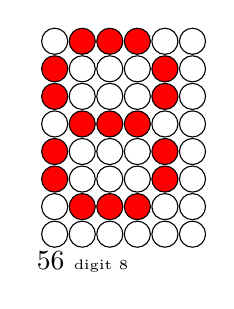
\begin{tikzpicture}[x=3.5mm,y=3.5mm]
\node [right] at (0,0) {56 {\tiny digit 8}};
\node [circle, fill=none, draw=black, minimum size=3mm] at (1,8) {};
\node [circle, fill=red, draw=black, minimum size=3mm] at (2,8) {};
\node [circle, fill=red, draw=black, minimum size=3mm] at (3,8) {};
\node [circle, fill=red, draw=black, minimum size=3mm] at (4,8) {};
\node [circle, fill=none, draw=black, minimum size=3mm] at (5,8) {};
\node [circle, fill=none, draw=black, minimum size=3mm] at (6,8) {};
\node [circle, fill=red, draw=black, minimum size=3mm] at (1,7) {};
\node [circle, fill=none, draw=black, minimum size=3mm] at (2,7) {};
\node [circle, fill=none, draw=black, minimum size=3mm] at (3,7) {};
\node [circle, fill=none, draw=black, minimum size=3mm] at (4,7) {};
\node [circle, fill=red, draw=black, minimum size=3mm] at (5,7) {};
\node [circle, fill=none, draw=black, minimum size=3mm] at (6,7) {};
\node [circle, fill=red, draw=black, minimum size=3mm] at (1,6) {};
\node [circle, fill=none, draw=black, minimum size=3mm] at (2,6) {};
\node [circle, fill=none, draw=black, minimum size=3mm] at (3,6) {};
\node [circle, fill=none, draw=black, minimum size=3mm] at (4,6) {};
\node [circle, fill=red, draw=black, minimum size=3mm] at (5,6) {};
\node [circle, fill=none, draw=black, minimum size=3mm] at (6,6) {};
\node [circle, fill=none, draw=black, minimum size=3mm] at (1,5) {};
\node [circle, fill=red, draw=black, minimum size=3mm] at (2,5) {};
\node [circle, fill=red, draw=black, minimum size=3mm] at (3,5) {};
\node [circle, fill=red, draw=black, minimum size=3mm] at (4,5) {};
\node [circle, fill=none, draw=black, minimum size=3mm] at (5,5) {};
\node [circle, fill=none, draw=black, minimum size=3mm] at (6,5) {};
\node [circle, fill=red, draw=black, minimum size=3mm] at (1,4) {};
\node [circle, fill=none, draw=black, minimum size=3mm] at (2,4) {};
\node [circle, fill=none, draw=black, minimum size=3mm] at (3,4) {};
\node [circle, fill=none, draw=black, minimum size=3mm] at (4,4) {};
\node [circle, fill=red, draw=black, minimum size=3mm] at (5,4) {};
\node [circle, fill=none, draw=black, minimum size=3mm] at (6,4) {};
\node [circle, fill=red, draw=black, minimum size=3mm] at (1,3) {};
\node [circle, fill=none, draw=black, minimum size=3mm] at (2,3) {};
\node [circle, fill=none, draw=black, minimum size=3mm] at (3,3) {};
\node [circle, fill=none, draw=black, minimum size=3mm] at (4,3) {};
\node [circle, fill=red, draw=black, minimum size=3mm] at (5,3) {};
\node [circle, fill=none, draw=black, minimum size=3mm] at (6,3) {};
\node [circle, fill=none, draw=black, minimum size=3mm] at (1,2) {};
\node [circle, fill=red, draw=black, minimum size=3mm] at (2,2) {};
\node [circle, fill=red, draw=black, minimum size=3mm] at (3,2) {};
\node [circle, fill=red, draw=black, minimum size=3mm] at (4,2) {};
\node [circle, fill=none, draw=black, minimum size=3mm] at (5,2) {};
\node [circle, fill=none, draw=black, minimum size=3mm] at (6,2) {};
\node [circle, fill=none, draw=black, minimum size=3mm] at (1,1) {};
\node [circle, fill=none, draw=black, minimum size=3mm] at (2,1) {};
\node [circle, fill=none, draw=black, minimum size=3mm] at (3,1) {};
\node [circle, fill=none, draw=black, minimum size=3mm] at (4,1) {};
\node [circle, fill=none, draw=black, minimum size=3mm] at (5,1) {};
\node [circle, fill=none, draw=black, minimum size=3mm] at (6,1) {};
\end{tikzpicture}% font 0 codepoint 57 name digit 9 space 6 width 5 offset 112


\noindent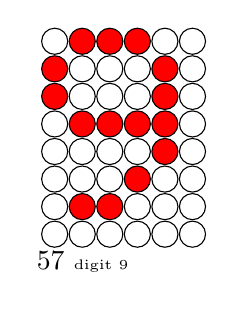
\begin{tikzpicture}[x=3.5mm,y=3.5mm]
\node [right] at (0,0) {57 {\tiny digit 9}};
\node [circle, fill=none, draw=black, minimum size=3mm] at (1,8) {};
\node [circle, fill=red, draw=black, minimum size=3mm] at (2,8) {};
\node [circle, fill=red, draw=black, minimum size=3mm] at (3,8) {};
\node [circle, fill=red, draw=black, minimum size=3mm] at (4,8) {};
\node [circle, fill=none, draw=black, minimum size=3mm] at (5,8) {};
\node [circle, fill=none, draw=black, minimum size=3mm] at (6,8) {};
\node [circle, fill=red, draw=black, minimum size=3mm] at (1,7) {};
\node [circle, fill=none, draw=black, minimum size=3mm] at (2,7) {};
\node [circle, fill=none, draw=black, minimum size=3mm] at (3,7) {};
\node [circle, fill=none, draw=black, minimum size=3mm] at (4,7) {};
\node [circle, fill=red, draw=black, minimum size=3mm] at (5,7) {};
\node [circle, fill=none, draw=black, minimum size=3mm] at (6,7) {};
\node [circle, fill=red, draw=black, minimum size=3mm] at (1,6) {};
\node [circle, fill=none, draw=black, minimum size=3mm] at (2,6) {};
\node [circle, fill=none, draw=black, minimum size=3mm] at (3,6) {};
\node [circle, fill=none, draw=black, minimum size=3mm] at (4,6) {};
\node [circle, fill=red, draw=black, minimum size=3mm] at (5,6) {};
\node [circle, fill=none, draw=black, minimum size=3mm] at (6,6) {};
\node [circle, fill=none, draw=black, minimum size=3mm] at (1,5) {};
\node [circle, fill=red, draw=black, minimum size=3mm] at (2,5) {};
\node [circle, fill=red, draw=black, minimum size=3mm] at (3,5) {};
\node [circle, fill=red, draw=black, minimum size=3mm] at (4,5) {};
\node [circle, fill=red, draw=black, minimum size=3mm] at (5,5) {};
\node [circle, fill=none, draw=black, minimum size=3mm] at (6,5) {};
\node [circle, fill=none, draw=black, minimum size=3mm] at (1,4) {};
\node [circle, fill=none, draw=black, minimum size=3mm] at (2,4) {};
\node [circle, fill=none, draw=black, minimum size=3mm] at (3,4) {};
\node [circle, fill=none, draw=black, minimum size=3mm] at (4,4) {};
\node [circle, fill=red, draw=black, minimum size=3mm] at (5,4) {};
\node [circle, fill=none, draw=black, minimum size=3mm] at (6,4) {};
\node [circle, fill=none, draw=black, minimum size=3mm] at (1,3) {};
\node [circle, fill=none, draw=black, minimum size=3mm] at (2,3) {};
\node [circle, fill=none, draw=black, minimum size=3mm] at (3,3) {};
\node [circle, fill=red, draw=black, minimum size=3mm] at (4,3) {};
\node [circle, fill=none, draw=black, minimum size=3mm] at (5,3) {};
\node [circle, fill=none, draw=black, minimum size=3mm] at (6,3) {};
\node [circle, fill=none, draw=black, minimum size=3mm] at (1,2) {};
\node [circle, fill=red, draw=black, minimum size=3mm] at (2,2) {};
\node [circle, fill=red, draw=black, minimum size=3mm] at (3,2) {};
\node [circle, fill=none, draw=black, minimum size=3mm] at (4,2) {};
\node [circle, fill=none, draw=black, minimum size=3mm] at (5,2) {};
\node [circle, fill=none, draw=black, minimum size=3mm] at (6,2) {};
\node [circle, fill=none, draw=black, minimum size=3mm] at (1,1) {};
\node [circle, fill=none, draw=black, minimum size=3mm] at (2,1) {};
\node [circle, fill=none, draw=black, minimum size=3mm] at (3,1) {};
\node [circle, fill=none, draw=black, minimum size=3mm] at (4,1) {};
\node [circle, fill=none, draw=black, minimum size=3mm] at (5,1) {};
\node [circle, fill=none, draw=black, minimum size=3mm] at (6,1) {};
\end{tikzpicture}% font 0 codepoint 58 name colon space 6 width 2 offset 117
~ 
\noindent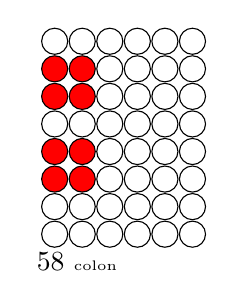
\begin{tikzpicture}[x=3.5mm,y=3.5mm]
\node [right] at (0,0) {58 {\tiny colon}};
\node [circle, fill=none, draw=black, minimum size=3mm] at (1,8) {};
\node [circle, fill=none, draw=black, minimum size=3mm] at (2,8) {};
\node [circle, fill=none, draw=black, minimum size=3mm] at (3,8) {};
\node [circle, fill=none, draw=black, minimum size=3mm] at (4,8) {};
\node [circle, fill=none, draw=black, minimum size=3mm] at (5,8) {};
\node [circle, fill=none, draw=black, minimum size=3mm] at (6,8) {};
\node [circle, fill=red, draw=black, minimum size=3mm] at (1,7) {};
\node [circle, fill=red, draw=black, minimum size=3mm] at (2,7) {};
\node [circle, fill=none, draw=black, minimum size=3mm] at (3,7) {};
\node [circle, fill=none, draw=black, minimum size=3mm] at (4,7) {};
\node [circle, fill=none, draw=black, minimum size=3mm] at (5,7) {};
\node [circle, fill=none, draw=black, minimum size=3mm] at (6,7) {};
\node [circle, fill=red, draw=black, minimum size=3mm] at (1,6) {};
\node [circle, fill=red, draw=black, minimum size=3mm] at (2,6) {};
\node [circle, fill=none, draw=black, minimum size=3mm] at (3,6) {};
\node [circle, fill=none, draw=black, minimum size=3mm] at (4,6) {};
\node [circle, fill=none, draw=black, minimum size=3mm] at (5,6) {};
\node [circle, fill=none, draw=black, minimum size=3mm] at (6,6) {};
\node [circle, fill=none, draw=black, minimum size=3mm] at (1,5) {};
\node [circle, fill=none, draw=black, minimum size=3mm] at (2,5) {};
\node [circle, fill=none, draw=black, minimum size=3mm] at (3,5) {};
\node [circle, fill=none, draw=black, minimum size=3mm] at (4,5) {};
\node [circle, fill=none, draw=black, minimum size=3mm] at (5,5) {};
\node [circle, fill=none, draw=black, minimum size=3mm] at (6,5) {};
\node [circle, fill=red, draw=black, minimum size=3mm] at (1,4) {};
\node [circle, fill=red, draw=black, minimum size=3mm] at (2,4) {};
\node [circle, fill=none, draw=black, minimum size=3mm] at (3,4) {};
\node [circle, fill=none, draw=black, minimum size=3mm] at (4,4) {};
\node [circle, fill=none, draw=black, minimum size=3mm] at (5,4) {};
\node [circle, fill=none, draw=black, minimum size=3mm] at (6,4) {};
\node [circle, fill=red, draw=black, minimum size=3mm] at (1,3) {};
\node [circle, fill=red, draw=black, minimum size=3mm] at (2,3) {};
\node [circle, fill=none, draw=black, minimum size=3mm] at (3,3) {};
\node [circle, fill=none, draw=black, minimum size=3mm] at (4,3) {};
\node [circle, fill=none, draw=black, minimum size=3mm] at (5,3) {};
\node [circle, fill=none, draw=black, minimum size=3mm] at (6,3) {};
\node [circle, fill=none, draw=black, minimum size=3mm] at (1,2) {};
\node [circle, fill=none, draw=black, minimum size=3mm] at (2,2) {};
\node [circle, fill=none, draw=black, minimum size=3mm] at (3,2) {};
\node [circle, fill=none, draw=black, minimum size=3mm] at (4,2) {};
\node [circle, fill=none, draw=black, minimum size=3mm] at (5,2) {};
\node [circle, fill=none, draw=black, minimum size=3mm] at (6,2) {};
\node [circle, fill=none, draw=black, minimum size=3mm] at (1,1) {};
\node [circle, fill=none, draw=black, minimum size=3mm] at (2,1) {};
\node [circle, fill=none, draw=black, minimum size=3mm] at (3,1) {};
\node [circle, fill=none, draw=black, minimum size=3mm] at (4,1) {};
\node [circle, fill=none, draw=black, minimum size=3mm] at (5,1) {};
\node [circle, fill=none, draw=black, minimum size=3mm] at (6,1) {};
\end{tikzpicture}% font 0 codepoint 59 name semi-colon space 6 width 2 offset 119
~ 
\noindent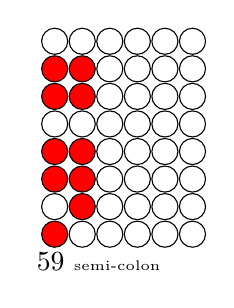
\begin{tikzpicture}[x=3.5mm,y=3.5mm]
\node [right] at (0,0) {59 {\tiny semi-colon}};
\node [circle, fill=none, draw=black, minimum size=3mm] at (1,8) {};
\node [circle, fill=none, draw=black, minimum size=3mm] at (2,8) {};
\node [circle, fill=none, draw=black, minimum size=3mm] at (3,8) {};
\node [circle, fill=none, draw=black, minimum size=3mm] at (4,8) {};
\node [circle, fill=none, draw=black, minimum size=3mm] at (5,8) {};
\node [circle, fill=none, draw=black, minimum size=3mm] at (6,8) {};
\node [circle, fill=red, draw=black, minimum size=3mm] at (1,7) {};
\node [circle, fill=red, draw=black, minimum size=3mm] at (2,7) {};
\node [circle, fill=none, draw=black, minimum size=3mm] at (3,7) {};
\node [circle, fill=none, draw=black, minimum size=3mm] at (4,7) {};
\node [circle, fill=none, draw=black, minimum size=3mm] at (5,7) {};
\node [circle, fill=none, draw=black, minimum size=3mm] at (6,7) {};
\node [circle, fill=red, draw=black, minimum size=3mm] at (1,6) {};
\node [circle, fill=red, draw=black, minimum size=3mm] at (2,6) {};
\node [circle, fill=none, draw=black, minimum size=3mm] at (3,6) {};
\node [circle, fill=none, draw=black, minimum size=3mm] at (4,6) {};
\node [circle, fill=none, draw=black, minimum size=3mm] at (5,6) {};
\node [circle, fill=none, draw=black, minimum size=3mm] at (6,6) {};
\node [circle, fill=none, draw=black, minimum size=3mm] at (1,5) {};
\node [circle, fill=none, draw=black, minimum size=3mm] at (2,5) {};
\node [circle, fill=none, draw=black, minimum size=3mm] at (3,5) {};
\node [circle, fill=none, draw=black, minimum size=3mm] at (4,5) {};
\node [circle, fill=none, draw=black, minimum size=3mm] at (5,5) {};
\node [circle, fill=none, draw=black, minimum size=3mm] at (6,5) {};
\node [circle, fill=red, draw=black, minimum size=3mm] at (1,4) {};
\node [circle, fill=red, draw=black, minimum size=3mm] at (2,4) {};
\node [circle, fill=none, draw=black, minimum size=3mm] at (3,4) {};
\node [circle, fill=none, draw=black, minimum size=3mm] at (4,4) {};
\node [circle, fill=none, draw=black, minimum size=3mm] at (5,4) {};
\node [circle, fill=none, draw=black, minimum size=3mm] at (6,4) {};
\node [circle, fill=red, draw=black, minimum size=3mm] at (1,3) {};
\node [circle, fill=red, draw=black, minimum size=3mm] at (2,3) {};
\node [circle, fill=none, draw=black, minimum size=3mm] at (3,3) {};
\node [circle, fill=none, draw=black, minimum size=3mm] at (4,3) {};
\node [circle, fill=none, draw=black, minimum size=3mm] at (5,3) {};
\node [circle, fill=none, draw=black, minimum size=3mm] at (6,3) {};
\node [circle, fill=none, draw=black, minimum size=3mm] at (1,2) {};
\node [circle, fill=red, draw=black, minimum size=3mm] at (2,2) {};
\node [circle, fill=none, draw=black, minimum size=3mm] at (3,2) {};
\node [circle, fill=none, draw=black, minimum size=3mm] at (4,2) {};
\node [circle, fill=none, draw=black, minimum size=3mm] at (5,2) {};
\node [circle, fill=none, draw=black, minimum size=3mm] at (6,2) {};
\node [circle, fill=red, draw=black, minimum size=3mm] at (1,1) {};
\node [circle, fill=none, draw=black, minimum size=3mm] at (2,1) {};
\node [circle, fill=none, draw=black, minimum size=3mm] at (3,1) {};
\node [circle, fill=none, draw=black, minimum size=3mm] at (4,1) {};
\node [circle, fill=none, draw=black, minimum size=3mm] at (5,1) {};
\node [circle, fill=none, draw=black, minimum size=3mm] at (6,1) {};
\end{tikzpicture}% font 0 codepoint 60 name less than space 6 width 4 offset 121
~ 
\noindent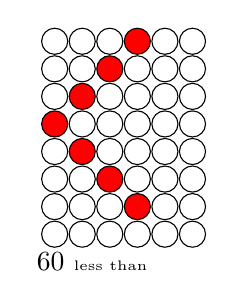
\begin{tikzpicture}[x=3.5mm,y=3.5mm]
\node [right] at (0,0) {60 {\tiny less than}};
\node [circle, fill=none, draw=black, minimum size=3mm] at (1,8) {};
\node [circle, fill=none, draw=black, minimum size=3mm] at (2,8) {};
\node [circle, fill=none, draw=black, minimum size=3mm] at (3,8) {};
\node [circle, fill=red, draw=black, minimum size=3mm] at (4,8) {};
\node [circle, fill=none, draw=black, minimum size=3mm] at (5,8) {};
\node [circle, fill=none, draw=black, minimum size=3mm] at (6,8) {};
\node [circle, fill=none, draw=black, minimum size=3mm] at (1,7) {};
\node [circle, fill=none, draw=black, minimum size=3mm] at (2,7) {};
\node [circle, fill=red, draw=black, minimum size=3mm] at (3,7) {};
\node [circle, fill=none, draw=black, minimum size=3mm] at (4,7) {};
\node [circle, fill=none, draw=black, minimum size=3mm] at (5,7) {};
\node [circle, fill=none, draw=black, minimum size=3mm] at (6,7) {};
\node [circle, fill=none, draw=black, minimum size=3mm] at (1,6) {};
\node [circle, fill=red, draw=black, minimum size=3mm] at (2,6) {};
\node [circle, fill=none, draw=black, minimum size=3mm] at (3,6) {};
\node [circle, fill=none, draw=black, minimum size=3mm] at (4,6) {};
\node [circle, fill=none, draw=black, minimum size=3mm] at (5,6) {};
\node [circle, fill=none, draw=black, minimum size=3mm] at (6,6) {};
\node [circle, fill=red, draw=black, minimum size=3mm] at (1,5) {};
\node [circle, fill=none, draw=black, minimum size=3mm] at (2,5) {};
\node [circle, fill=none, draw=black, minimum size=3mm] at (3,5) {};
\node [circle, fill=none, draw=black, minimum size=3mm] at (4,5) {};
\node [circle, fill=none, draw=black, minimum size=3mm] at (5,5) {};
\node [circle, fill=none, draw=black, minimum size=3mm] at (6,5) {};
\node [circle, fill=none, draw=black, minimum size=3mm] at (1,4) {};
\node [circle, fill=red, draw=black, minimum size=3mm] at (2,4) {};
\node [circle, fill=none, draw=black, minimum size=3mm] at (3,4) {};
\node [circle, fill=none, draw=black, minimum size=3mm] at (4,4) {};
\node [circle, fill=none, draw=black, minimum size=3mm] at (5,4) {};
\node [circle, fill=none, draw=black, minimum size=3mm] at (6,4) {};
\node [circle, fill=none, draw=black, minimum size=3mm] at (1,3) {};
\node [circle, fill=none, draw=black, minimum size=3mm] at (2,3) {};
\node [circle, fill=red, draw=black, minimum size=3mm] at (3,3) {};
\node [circle, fill=none, draw=black, minimum size=3mm] at (4,3) {};
\node [circle, fill=none, draw=black, minimum size=3mm] at (5,3) {};
\node [circle, fill=none, draw=black, minimum size=3mm] at (6,3) {};
\node [circle, fill=none, draw=black, minimum size=3mm] at (1,2) {};
\node [circle, fill=none, draw=black, minimum size=3mm] at (2,2) {};
\node [circle, fill=none, draw=black, minimum size=3mm] at (3,2) {};
\node [circle, fill=red, draw=black, minimum size=3mm] at (4,2) {};
\node [circle, fill=none, draw=black, minimum size=3mm] at (5,2) {};
\node [circle, fill=none, draw=black, minimum size=3mm] at (6,2) {};
\node [circle, fill=none, draw=black, minimum size=3mm] at (1,1) {};
\node [circle, fill=none, draw=black, minimum size=3mm] at (2,1) {};
\node [circle, fill=none, draw=black, minimum size=3mm] at (3,1) {};
\node [circle, fill=none, draw=black, minimum size=3mm] at (4,1) {};
\node [circle, fill=none, draw=black, minimum size=3mm] at (5,1) {};
\node [circle, fill=none, draw=black, minimum size=3mm] at (6,1) {};
\end{tikzpicture}% font 0 codepoint 61 name equals space 6 width 5 offset 125
~ 
\noindent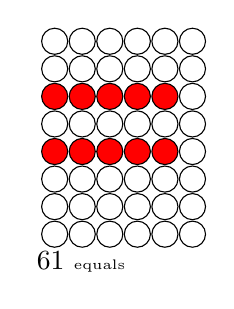
\begin{tikzpicture}[x=3.5mm,y=3.5mm]
\node [right] at (0,0) {61 {\tiny equals}};
\node [circle, fill=none, draw=black, minimum size=3mm] at (1,8) {};
\node [circle, fill=none, draw=black, minimum size=3mm] at (2,8) {};
\node [circle, fill=none, draw=black, minimum size=3mm] at (3,8) {};
\node [circle, fill=none, draw=black, minimum size=3mm] at (4,8) {};
\node [circle, fill=none, draw=black, minimum size=3mm] at (5,8) {};
\node [circle, fill=none, draw=black, minimum size=3mm] at (6,8) {};
\node [circle, fill=none, draw=black, minimum size=3mm] at (1,7) {};
\node [circle, fill=none, draw=black, minimum size=3mm] at (2,7) {};
\node [circle, fill=none, draw=black, minimum size=3mm] at (3,7) {};
\node [circle, fill=none, draw=black, minimum size=3mm] at (4,7) {};
\node [circle, fill=none, draw=black, minimum size=3mm] at (5,7) {};
\node [circle, fill=none, draw=black, minimum size=3mm] at (6,7) {};
\node [circle, fill=red, draw=black, minimum size=3mm] at (1,6) {};
\node [circle, fill=red, draw=black, minimum size=3mm] at (2,6) {};
\node [circle, fill=red, draw=black, minimum size=3mm] at (3,6) {};
\node [circle, fill=red, draw=black, minimum size=3mm] at (4,6) {};
\node [circle, fill=red, draw=black, minimum size=3mm] at (5,6) {};
\node [circle, fill=none, draw=black, minimum size=3mm] at (6,6) {};
\node [circle, fill=none, draw=black, minimum size=3mm] at (1,5) {};
\node [circle, fill=none, draw=black, minimum size=3mm] at (2,5) {};
\node [circle, fill=none, draw=black, minimum size=3mm] at (3,5) {};
\node [circle, fill=none, draw=black, minimum size=3mm] at (4,5) {};
\node [circle, fill=none, draw=black, minimum size=3mm] at (5,5) {};
\node [circle, fill=none, draw=black, minimum size=3mm] at (6,5) {};
\node [circle, fill=red, draw=black, minimum size=3mm] at (1,4) {};
\node [circle, fill=red, draw=black, minimum size=3mm] at (2,4) {};
\node [circle, fill=red, draw=black, minimum size=3mm] at (3,4) {};
\node [circle, fill=red, draw=black, minimum size=3mm] at (4,4) {};
\node [circle, fill=red, draw=black, minimum size=3mm] at (5,4) {};
\node [circle, fill=none, draw=black, minimum size=3mm] at (6,4) {};
\node [circle, fill=none, draw=black, minimum size=3mm] at (1,3) {};
\node [circle, fill=none, draw=black, minimum size=3mm] at (2,3) {};
\node [circle, fill=none, draw=black, minimum size=3mm] at (3,3) {};
\node [circle, fill=none, draw=black, minimum size=3mm] at (4,3) {};
\node [circle, fill=none, draw=black, minimum size=3mm] at (5,3) {};
\node [circle, fill=none, draw=black, minimum size=3mm] at (6,3) {};
\node [circle, fill=none, draw=black, minimum size=3mm] at (1,2) {};
\node [circle, fill=none, draw=black, minimum size=3mm] at (2,2) {};
\node [circle, fill=none, draw=black, minimum size=3mm] at (3,2) {};
\node [circle, fill=none, draw=black, minimum size=3mm] at (4,2) {};
\node [circle, fill=none, draw=black, minimum size=3mm] at (5,2) {};
\node [circle, fill=none, draw=black, minimum size=3mm] at (6,2) {};
\node [circle, fill=none, draw=black, minimum size=3mm] at (1,1) {};
\node [circle, fill=none, draw=black, minimum size=3mm] at (2,1) {};
\node [circle, fill=none, draw=black, minimum size=3mm] at (3,1) {};
\node [circle, fill=none, draw=black, minimum size=3mm] at (4,1) {};
\node [circle, fill=none, draw=black, minimum size=3mm] at (5,1) {};
\node [circle, fill=none, draw=black, minimum size=3mm] at (6,1) {};
\end{tikzpicture}% font 0 codepoint 62 name greater than space 6 width 5 offset 130


\noindent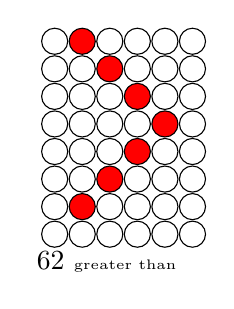
\begin{tikzpicture}[x=3.5mm,y=3.5mm]
\node [right] at (0,0) {62 {\tiny greater than}};
\node [circle, fill=none, draw=black, minimum size=3mm] at (1,8) {};
\node [circle, fill=red, draw=black, minimum size=3mm] at (2,8) {};
\node [circle, fill=none, draw=black, minimum size=3mm] at (3,8) {};
\node [circle, fill=none, draw=black, minimum size=3mm] at (4,8) {};
\node [circle, fill=none, draw=black, minimum size=3mm] at (5,8) {};
\node [circle, fill=none, draw=black, minimum size=3mm] at (6,8) {};
\node [circle, fill=none, draw=black, minimum size=3mm] at (1,7) {};
\node [circle, fill=none, draw=black, minimum size=3mm] at (2,7) {};
\node [circle, fill=red, draw=black, minimum size=3mm] at (3,7) {};
\node [circle, fill=none, draw=black, minimum size=3mm] at (4,7) {};
\node [circle, fill=none, draw=black, minimum size=3mm] at (5,7) {};
\node [circle, fill=none, draw=black, minimum size=3mm] at (6,7) {};
\node [circle, fill=none, draw=black, minimum size=3mm] at (1,6) {};
\node [circle, fill=none, draw=black, minimum size=3mm] at (2,6) {};
\node [circle, fill=none, draw=black, minimum size=3mm] at (3,6) {};
\node [circle, fill=red, draw=black, minimum size=3mm] at (4,6) {};
\node [circle, fill=none, draw=black, minimum size=3mm] at (5,6) {};
\node [circle, fill=none, draw=black, minimum size=3mm] at (6,6) {};
\node [circle, fill=none, draw=black, minimum size=3mm] at (1,5) {};
\node [circle, fill=none, draw=black, minimum size=3mm] at (2,5) {};
\node [circle, fill=none, draw=black, minimum size=3mm] at (3,5) {};
\node [circle, fill=none, draw=black, minimum size=3mm] at (4,5) {};
\node [circle, fill=red, draw=black, minimum size=3mm] at (5,5) {};
\node [circle, fill=none, draw=black, minimum size=3mm] at (6,5) {};
\node [circle, fill=none, draw=black, minimum size=3mm] at (1,4) {};
\node [circle, fill=none, draw=black, minimum size=3mm] at (2,4) {};
\node [circle, fill=none, draw=black, minimum size=3mm] at (3,4) {};
\node [circle, fill=red, draw=black, minimum size=3mm] at (4,4) {};
\node [circle, fill=none, draw=black, minimum size=3mm] at (5,4) {};
\node [circle, fill=none, draw=black, minimum size=3mm] at (6,4) {};
\node [circle, fill=none, draw=black, minimum size=3mm] at (1,3) {};
\node [circle, fill=none, draw=black, minimum size=3mm] at (2,3) {};
\node [circle, fill=red, draw=black, minimum size=3mm] at (3,3) {};
\node [circle, fill=none, draw=black, minimum size=3mm] at (4,3) {};
\node [circle, fill=none, draw=black, minimum size=3mm] at (5,3) {};
\node [circle, fill=none, draw=black, minimum size=3mm] at (6,3) {};
\node [circle, fill=none, draw=black, minimum size=3mm] at (1,2) {};
\node [circle, fill=red, draw=black, minimum size=3mm] at (2,2) {};
\node [circle, fill=none, draw=black, minimum size=3mm] at (3,2) {};
\node [circle, fill=none, draw=black, minimum size=3mm] at (4,2) {};
\node [circle, fill=none, draw=black, minimum size=3mm] at (5,2) {};
\node [circle, fill=none, draw=black, minimum size=3mm] at (6,2) {};
\node [circle, fill=none, draw=black, minimum size=3mm] at (1,1) {};
\node [circle, fill=none, draw=black, minimum size=3mm] at (2,1) {};
\node [circle, fill=none, draw=black, minimum size=3mm] at (3,1) {};
\node [circle, fill=none, draw=black, minimum size=3mm] at (4,1) {};
\node [circle, fill=none, draw=black, minimum size=3mm] at (5,1) {};
\node [circle, fill=none, draw=black, minimum size=3mm] at (6,1) {};
\end{tikzpicture}% font 0 codepoint 63 name question mark space 6 width 5 offset 135
~ 
\noindent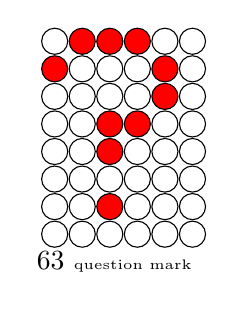
\begin{tikzpicture}[x=3.5mm,y=3.5mm]
\node [right] at (0,0) {63 {\tiny question mark}};
\node [circle, fill=none, draw=black, minimum size=3mm] at (1,8) {};
\node [circle, fill=red, draw=black, minimum size=3mm] at (2,8) {};
\node [circle, fill=red, draw=black, minimum size=3mm] at (3,8) {};
\node [circle, fill=red, draw=black, minimum size=3mm] at (4,8) {};
\node [circle, fill=none, draw=black, minimum size=3mm] at (5,8) {};
\node [circle, fill=none, draw=black, minimum size=3mm] at (6,8) {};
\node [circle, fill=red, draw=black, minimum size=3mm] at (1,7) {};
\node [circle, fill=none, draw=black, minimum size=3mm] at (2,7) {};
\node [circle, fill=none, draw=black, minimum size=3mm] at (3,7) {};
\node [circle, fill=none, draw=black, minimum size=3mm] at (4,7) {};
\node [circle, fill=red, draw=black, minimum size=3mm] at (5,7) {};
\node [circle, fill=none, draw=black, minimum size=3mm] at (6,7) {};
\node [circle, fill=none, draw=black, minimum size=3mm] at (1,6) {};
\node [circle, fill=none, draw=black, minimum size=3mm] at (2,6) {};
\node [circle, fill=none, draw=black, minimum size=3mm] at (3,6) {};
\node [circle, fill=none, draw=black, minimum size=3mm] at (4,6) {};
\node [circle, fill=red, draw=black, minimum size=3mm] at (5,6) {};
\node [circle, fill=none, draw=black, minimum size=3mm] at (6,6) {};
\node [circle, fill=none, draw=black, minimum size=3mm] at (1,5) {};
\node [circle, fill=none, draw=black, minimum size=3mm] at (2,5) {};
\node [circle, fill=red, draw=black, minimum size=3mm] at (3,5) {};
\node [circle, fill=red, draw=black, minimum size=3mm] at (4,5) {};
\node [circle, fill=none, draw=black, minimum size=3mm] at (5,5) {};
\node [circle, fill=none, draw=black, minimum size=3mm] at (6,5) {};
\node [circle, fill=none, draw=black, minimum size=3mm] at (1,4) {};
\node [circle, fill=none, draw=black, minimum size=3mm] at (2,4) {};
\node [circle, fill=red, draw=black, minimum size=3mm] at (3,4) {};
\node [circle, fill=none, draw=black, minimum size=3mm] at (4,4) {};
\node [circle, fill=none, draw=black, minimum size=3mm] at (5,4) {};
\node [circle, fill=none, draw=black, minimum size=3mm] at (6,4) {};
\node [circle, fill=none, draw=black, minimum size=3mm] at (1,3) {};
\node [circle, fill=none, draw=black, minimum size=3mm] at (2,3) {};
\node [circle, fill=none, draw=black, minimum size=3mm] at (3,3) {};
\node [circle, fill=none, draw=black, minimum size=3mm] at (4,3) {};
\node [circle, fill=none, draw=black, minimum size=3mm] at (5,3) {};
\node [circle, fill=none, draw=black, minimum size=3mm] at (6,3) {};
\node [circle, fill=none, draw=black, minimum size=3mm] at (1,2) {};
\node [circle, fill=none, draw=black, minimum size=3mm] at (2,2) {};
\node [circle, fill=red, draw=black, minimum size=3mm] at (3,2) {};
\node [circle, fill=none, draw=black, minimum size=3mm] at (4,2) {};
\node [circle, fill=none, draw=black, minimum size=3mm] at (5,2) {};
\node [circle, fill=none, draw=black, minimum size=3mm] at (6,2) {};
\node [circle, fill=none, draw=black, minimum size=3mm] at (1,1) {};
\node [circle, fill=none, draw=black, minimum size=3mm] at (2,1) {};
\node [circle, fill=none, draw=black, minimum size=3mm] at (3,1) {};
\node [circle, fill=none, draw=black, minimum size=3mm] at (4,1) {};
\node [circle, fill=none, draw=black, minimum size=3mm] at (5,1) {};
\node [circle, fill=none, draw=black, minimum size=3mm] at (6,1) {};
\end{tikzpicture}% font 0 codepoint 64 name at-sign space 6 width 5 offset 140
~ 
\noindent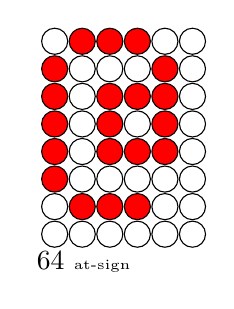
\begin{tikzpicture}[x=3.5mm,y=3.5mm]
\node [right] at (0,0) {64 {\tiny at-sign}};
\node [circle, fill=none, draw=black, minimum size=3mm] at (1,8) {};
\node [circle, fill=red, draw=black, minimum size=3mm] at (2,8) {};
\node [circle, fill=red, draw=black, minimum size=3mm] at (3,8) {};
\node [circle, fill=red, draw=black, minimum size=3mm] at (4,8) {};
\node [circle, fill=none, draw=black, minimum size=3mm] at (5,8) {};
\node [circle, fill=none, draw=black, minimum size=3mm] at (6,8) {};
\node [circle, fill=red, draw=black, minimum size=3mm] at (1,7) {};
\node [circle, fill=none, draw=black, minimum size=3mm] at (2,7) {};
\node [circle, fill=none, draw=black, minimum size=3mm] at (3,7) {};
\node [circle, fill=none, draw=black, minimum size=3mm] at (4,7) {};
\node [circle, fill=red, draw=black, minimum size=3mm] at (5,7) {};
\node [circle, fill=none, draw=black, minimum size=3mm] at (6,7) {};
\node [circle, fill=red, draw=black, minimum size=3mm] at (1,6) {};
\node [circle, fill=none, draw=black, minimum size=3mm] at (2,6) {};
\node [circle, fill=red, draw=black, minimum size=3mm] at (3,6) {};
\node [circle, fill=red, draw=black, minimum size=3mm] at (4,6) {};
\node [circle, fill=red, draw=black, minimum size=3mm] at (5,6) {};
\node [circle, fill=none, draw=black, minimum size=3mm] at (6,6) {};
\node [circle, fill=red, draw=black, minimum size=3mm] at (1,5) {};
\node [circle, fill=none, draw=black, minimum size=3mm] at (2,5) {};
\node [circle, fill=red, draw=black, minimum size=3mm] at (3,5) {};
\node [circle, fill=none, draw=black, minimum size=3mm] at (4,5) {};
\node [circle, fill=red, draw=black, minimum size=3mm] at (5,5) {};
\node [circle, fill=none, draw=black, minimum size=3mm] at (6,5) {};
\node [circle, fill=red, draw=black, minimum size=3mm] at (1,4) {};
\node [circle, fill=none, draw=black, minimum size=3mm] at (2,4) {};
\node [circle, fill=red, draw=black, minimum size=3mm] at (3,4) {};
\node [circle, fill=red, draw=black, minimum size=3mm] at (4,4) {};
\node [circle, fill=red, draw=black, minimum size=3mm] at (5,4) {};
\node [circle, fill=none, draw=black, minimum size=3mm] at (6,4) {};
\node [circle, fill=red, draw=black, minimum size=3mm] at (1,3) {};
\node [circle, fill=none, draw=black, minimum size=3mm] at (2,3) {};
\node [circle, fill=none, draw=black, minimum size=3mm] at (3,3) {};
\node [circle, fill=none, draw=black, minimum size=3mm] at (4,3) {};
\node [circle, fill=none, draw=black, minimum size=3mm] at (5,3) {};
\node [circle, fill=none, draw=black, minimum size=3mm] at (6,3) {};
\node [circle, fill=none, draw=black, minimum size=3mm] at (1,2) {};
\node [circle, fill=red, draw=black, minimum size=3mm] at (2,2) {};
\node [circle, fill=red, draw=black, minimum size=3mm] at (3,2) {};
\node [circle, fill=red, draw=black, minimum size=3mm] at (4,2) {};
\node [circle, fill=none, draw=black, minimum size=3mm] at (5,2) {};
\node [circle, fill=none, draw=black, minimum size=3mm] at (6,2) {};
\node [circle, fill=none, draw=black, minimum size=3mm] at (1,1) {};
\node [circle, fill=none, draw=black, minimum size=3mm] at (2,1) {};
\node [circle, fill=none, draw=black, minimum size=3mm] at (3,1) {};
\node [circle, fill=none, draw=black, minimum size=3mm] at (4,1) {};
\node [circle, fill=none, draw=black, minimum size=3mm] at (5,1) {};
\node [circle, fill=none, draw=black, minimum size=3mm] at (6,1) {};
\end{tikzpicture}% font 0 codepoint 65 name A space 6 width 5 offset 145
~ 
\noindent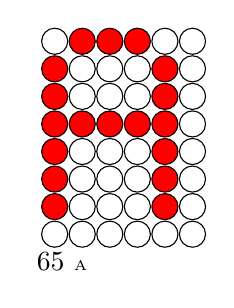
\begin{tikzpicture}[x=3.5mm,y=3.5mm]
\node [right] at (0,0) {65 {\tiny A}};
\node [circle, fill=none, draw=black, minimum size=3mm] at (1,8) {};
\node [circle, fill=red, draw=black, minimum size=3mm] at (2,8) {};
\node [circle, fill=red, draw=black, minimum size=3mm] at (3,8) {};
\node [circle, fill=red, draw=black, minimum size=3mm] at (4,8) {};
\node [circle, fill=none, draw=black, minimum size=3mm] at (5,8) {};
\node [circle, fill=none, draw=black, minimum size=3mm] at (6,8) {};
\node [circle, fill=red, draw=black, minimum size=3mm] at (1,7) {};
\node [circle, fill=none, draw=black, minimum size=3mm] at (2,7) {};
\node [circle, fill=none, draw=black, minimum size=3mm] at (3,7) {};
\node [circle, fill=none, draw=black, minimum size=3mm] at (4,7) {};
\node [circle, fill=red, draw=black, minimum size=3mm] at (5,7) {};
\node [circle, fill=none, draw=black, minimum size=3mm] at (6,7) {};
\node [circle, fill=red, draw=black, minimum size=3mm] at (1,6) {};
\node [circle, fill=none, draw=black, minimum size=3mm] at (2,6) {};
\node [circle, fill=none, draw=black, minimum size=3mm] at (3,6) {};
\node [circle, fill=none, draw=black, minimum size=3mm] at (4,6) {};
\node [circle, fill=red, draw=black, minimum size=3mm] at (5,6) {};
\node [circle, fill=none, draw=black, minimum size=3mm] at (6,6) {};
\node [circle, fill=red, draw=black, minimum size=3mm] at (1,5) {};
\node [circle, fill=red, draw=black, minimum size=3mm] at (2,5) {};
\node [circle, fill=red, draw=black, minimum size=3mm] at (3,5) {};
\node [circle, fill=red, draw=black, minimum size=3mm] at (4,5) {};
\node [circle, fill=red, draw=black, minimum size=3mm] at (5,5) {};
\node [circle, fill=none, draw=black, minimum size=3mm] at (6,5) {};
\node [circle, fill=red, draw=black, minimum size=3mm] at (1,4) {};
\node [circle, fill=none, draw=black, minimum size=3mm] at (2,4) {};
\node [circle, fill=none, draw=black, minimum size=3mm] at (3,4) {};
\node [circle, fill=none, draw=black, minimum size=3mm] at (4,4) {};
\node [circle, fill=red, draw=black, minimum size=3mm] at (5,4) {};
\node [circle, fill=none, draw=black, minimum size=3mm] at (6,4) {};
\node [circle, fill=red, draw=black, minimum size=3mm] at (1,3) {};
\node [circle, fill=none, draw=black, minimum size=3mm] at (2,3) {};
\node [circle, fill=none, draw=black, minimum size=3mm] at (3,3) {};
\node [circle, fill=none, draw=black, minimum size=3mm] at (4,3) {};
\node [circle, fill=red, draw=black, minimum size=3mm] at (5,3) {};
\node [circle, fill=none, draw=black, minimum size=3mm] at (6,3) {};
\node [circle, fill=red, draw=black, minimum size=3mm] at (1,2) {};
\node [circle, fill=none, draw=black, minimum size=3mm] at (2,2) {};
\node [circle, fill=none, draw=black, minimum size=3mm] at (3,2) {};
\node [circle, fill=none, draw=black, minimum size=3mm] at (4,2) {};
\node [circle, fill=red, draw=black, minimum size=3mm] at (5,2) {};
\node [circle, fill=none, draw=black, minimum size=3mm] at (6,2) {};
\node [circle, fill=none, draw=black, minimum size=3mm] at (1,1) {};
\node [circle, fill=none, draw=black, minimum size=3mm] at (2,1) {};
\node [circle, fill=none, draw=black, minimum size=3mm] at (3,1) {};
\node [circle, fill=none, draw=black, minimum size=3mm] at (4,1) {};
\node [circle, fill=none, draw=black, minimum size=3mm] at (5,1) {};
\node [circle, fill=none, draw=black, minimum size=3mm] at (6,1) {};
\end{tikzpicture}% font 0 codepoint 66 name B space 6 width 5 offset 150
~ 
\noindent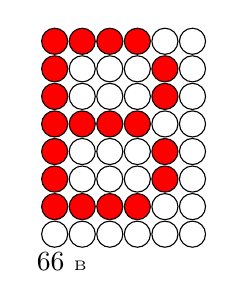
\begin{tikzpicture}[x=3.5mm,y=3.5mm]
\node [right] at (0,0) {66 {\tiny B}};
\node [circle, fill=red, draw=black, minimum size=3mm] at (1,8) {};
\node [circle, fill=red, draw=black, minimum size=3mm] at (2,8) {};
\node [circle, fill=red, draw=black, minimum size=3mm] at (3,8) {};
\node [circle, fill=red, draw=black, minimum size=3mm] at (4,8) {};
\node [circle, fill=none, draw=black, minimum size=3mm] at (5,8) {};
\node [circle, fill=none, draw=black, minimum size=3mm] at (6,8) {};
\node [circle, fill=red, draw=black, minimum size=3mm] at (1,7) {};
\node [circle, fill=none, draw=black, minimum size=3mm] at (2,7) {};
\node [circle, fill=none, draw=black, minimum size=3mm] at (3,7) {};
\node [circle, fill=none, draw=black, minimum size=3mm] at (4,7) {};
\node [circle, fill=red, draw=black, minimum size=3mm] at (5,7) {};
\node [circle, fill=none, draw=black, minimum size=3mm] at (6,7) {};
\node [circle, fill=red, draw=black, minimum size=3mm] at (1,6) {};
\node [circle, fill=none, draw=black, minimum size=3mm] at (2,6) {};
\node [circle, fill=none, draw=black, minimum size=3mm] at (3,6) {};
\node [circle, fill=none, draw=black, minimum size=3mm] at (4,6) {};
\node [circle, fill=red, draw=black, minimum size=3mm] at (5,6) {};
\node [circle, fill=none, draw=black, minimum size=3mm] at (6,6) {};
\node [circle, fill=red, draw=black, minimum size=3mm] at (1,5) {};
\node [circle, fill=red, draw=black, minimum size=3mm] at (2,5) {};
\node [circle, fill=red, draw=black, minimum size=3mm] at (3,5) {};
\node [circle, fill=red, draw=black, minimum size=3mm] at (4,5) {};
\node [circle, fill=none, draw=black, minimum size=3mm] at (5,5) {};
\node [circle, fill=none, draw=black, minimum size=3mm] at (6,5) {};
\node [circle, fill=red, draw=black, minimum size=3mm] at (1,4) {};
\node [circle, fill=none, draw=black, minimum size=3mm] at (2,4) {};
\node [circle, fill=none, draw=black, minimum size=3mm] at (3,4) {};
\node [circle, fill=none, draw=black, minimum size=3mm] at (4,4) {};
\node [circle, fill=red, draw=black, minimum size=3mm] at (5,4) {};
\node [circle, fill=none, draw=black, minimum size=3mm] at (6,4) {};
\node [circle, fill=red, draw=black, minimum size=3mm] at (1,3) {};
\node [circle, fill=none, draw=black, minimum size=3mm] at (2,3) {};
\node [circle, fill=none, draw=black, minimum size=3mm] at (3,3) {};
\node [circle, fill=none, draw=black, minimum size=3mm] at (4,3) {};
\node [circle, fill=red, draw=black, minimum size=3mm] at (5,3) {};
\node [circle, fill=none, draw=black, minimum size=3mm] at (6,3) {};
\node [circle, fill=red, draw=black, minimum size=3mm] at (1,2) {};
\node [circle, fill=red, draw=black, minimum size=3mm] at (2,2) {};
\node [circle, fill=red, draw=black, minimum size=3mm] at (3,2) {};
\node [circle, fill=red, draw=black, minimum size=3mm] at (4,2) {};
\node [circle, fill=none, draw=black, minimum size=3mm] at (5,2) {};
\node [circle, fill=none, draw=black, minimum size=3mm] at (6,2) {};
\node [circle, fill=none, draw=black, minimum size=3mm] at (1,1) {};
\node [circle, fill=none, draw=black, minimum size=3mm] at (2,1) {};
\node [circle, fill=none, draw=black, minimum size=3mm] at (3,1) {};
\node [circle, fill=none, draw=black, minimum size=3mm] at (4,1) {};
\node [circle, fill=none, draw=black, minimum size=3mm] at (5,1) {};
\node [circle, fill=none, draw=black, minimum size=3mm] at (6,1) {};
\end{tikzpicture}% font 0 codepoint 67 name C space 6 width 5 offset 155


\noindent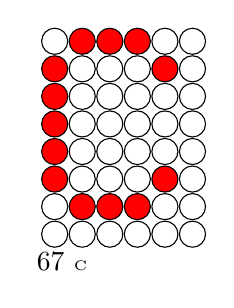
\begin{tikzpicture}[x=3.5mm,y=3.5mm]
\node [right] at (0,0) {67 {\tiny C}};
\node [circle, fill=none, draw=black, minimum size=3mm] at (1,8) {};
\node [circle, fill=red, draw=black, minimum size=3mm] at (2,8) {};
\node [circle, fill=red, draw=black, minimum size=3mm] at (3,8) {};
\node [circle, fill=red, draw=black, minimum size=3mm] at (4,8) {};
\node [circle, fill=none, draw=black, minimum size=3mm] at (5,8) {};
\node [circle, fill=none, draw=black, minimum size=3mm] at (6,8) {};
\node [circle, fill=red, draw=black, minimum size=3mm] at (1,7) {};
\node [circle, fill=none, draw=black, minimum size=3mm] at (2,7) {};
\node [circle, fill=none, draw=black, minimum size=3mm] at (3,7) {};
\node [circle, fill=none, draw=black, minimum size=3mm] at (4,7) {};
\node [circle, fill=red, draw=black, minimum size=3mm] at (5,7) {};
\node [circle, fill=none, draw=black, minimum size=3mm] at (6,7) {};
\node [circle, fill=red, draw=black, minimum size=3mm] at (1,6) {};
\node [circle, fill=none, draw=black, minimum size=3mm] at (2,6) {};
\node [circle, fill=none, draw=black, minimum size=3mm] at (3,6) {};
\node [circle, fill=none, draw=black, minimum size=3mm] at (4,6) {};
\node [circle, fill=none, draw=black, minimum size=3mm] at (5,6) {};
\node [circle, fill=none, draw=black, minimum size=3mm] at (6,6) {};
\node [circle, fill=red, draw=black, minimum size=3mm] at (1,5) {};
\node [circle, fill=none, draw=black, minimum size=3mm] at (2,5) {};
\node [circle, fill=none, draw=black, minimum size=3mm] at (3,5) {};
\node [circle, fill=none, draw=black, minimum size=3mm] at (4,5) {};
\node [circle, fill=none, draw=black, minimum size=3mm] at (5,5) {};
\node [circle, fill=none, draw=black, minimum size=3mm] at (6,5) {};
\node [circle, fill=red, draw=black, minimum size=3mm] at (1,4) {};
\node [circle, fill=none, draw=black, minimum size=3mm] at (2,4) {};
\node [circle, fill=none, draw=black, minimum size=3mm] at (3,4) {};
\node [circle, fill=none, draw=black, minimum size=3mm] at (4,4) {};
\node [circle, fill=none, draw=black, minimum size=3mm] at (5,4) {};
\node [circle, fill=none, draw=black, minimum size=3mm] at (6,4) {};
\node [circle, fill=red, draw=black, minimum size=3mm] at (1,3) {};
\node [circle, fill=none, draw=black, minimum size=3mm] at (2,3) {};
\node [circle, fill=none, draw=black, minimum size=3mm] at (3,3) {};
\node [circle, fill=none, draw=black, minimum size=3mm] at (4,3) {};
\node [circle, fill=red, draw=black, minimum size=3mm] at (5,3) {};
\node [circle, fill=none, draw=black, minimum size=3mm] at (6,3) {};
\node [circle, fill=none, draw=black, minimum size=3mm] at (1,2) {};
\node [circle, fill=red, draw=black, minimum size=3mm] at (2,2) {};
\node [circle, fill=red, draw=black, minimum size=3mm] at (3,2) {};
\node [circle, fill=red, draw=black, minimum size=3mm] at (4,2) {};
\node [circle, fill=none, draw=black, minimum size=3mm] at (5,2) {};
\node [circle, fill=none, draw=black, minimum size=3mm] at (6,2) {};
\node [circle, fill=none, draw=black, minimum size=3mm] at (1,1) {};
\node [circle, fill=none, draw=black, minimum size=3mm] at (2,1) {};
\node [circle, fill=none, draw=black, minimum size=3mm] at (3,1) {};
\node [circle, fill=none, draw=black, minimum size=3mm] at (4,1) {};
\node [circle, fill=none, draw=black, minimum size=3mm] at (5,1) {};
\node [circle, fill=none, draw=black, minimum size=3mm] at (6,1) {};
\end{tikzpicture}% font 0 codepoint 68 name D space 6 width 5 offset 160
~ 
\noindent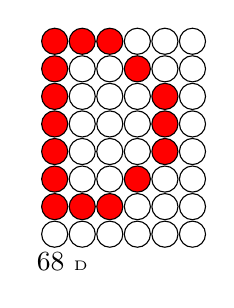
\begin{tikzpicture}[x=3.5mm,y=3.5mm]
\node [right] at (0,0) {68 {\tiny D}};
\node [circle, fill=red, draw=black, minimum size=3mm] at (1,8) {};
\node [circle, fill=red, draw=black, minimum size=3mm] at (2,8) {};
\node [circle, fill=red, draw=black, minimum size=3mm] at (3,8) {};
\node [circle, fill=none, draw=black, minimum size=3mm] at (4,8) {};
\node [circle, fill=none, draw=black, minimum size=3mm] at (5,8) {};
\node [circle, fill=none, draw=black, minimum size=3mm] at (6,8) {};
\node [circle, fill=red, draw=black, minimum size=3mm] at (1,7) {};
\node [circle, fill=none, draw=black, minimum size=3mm] at (2,7) {};
\node [circle, fill=none, draw=black, minimum size=3mm] at (3,7) {};
\node [circle, fill=red, draw=black, minimum size=3mm] at (4,7) {};
\node [circle, fill=none, draw=black, minimum size=3mm] at (5,7) {};
\node [circle, fill=none, draw=black, minimum size=3mm] at (6,7) {};
\node [circle, fill=red, draw=black, minimum size=3mm] at (1,6) {};
\node [circle, fill=none, draw=black, minimum size=3mm] at (2,6) {};
\node [circle, fill=none, draw=black, minimum size=3mm] at (3,6) {};
\node [circle, fill=none, draw=black, minimum size=3mm] at (4,6) {};
\node [circle, fill=red, draw=black, minimum size=3mm] at (5,6) {};
\node [circle, fill=none, draw=black, minimum size=3mm] at (6,6) {};
\node [circle, fill=red, draw=black, minimum size=3mm] at (1,5) {};
\node [circle, fill=none, draw=black, minimum size=3mm] at (2,5) {};
\node [circle, fill=none, draw=black, minimum size=3mm] at (3,5) {};
\node [circle, fill=none, draw=black, minimum size=3mm] at (4,5) {};
\node [circle, fill=red, draw=black, minimum size=3mm] at (5,5) {};
\node [circle, fill=none, draw=black, minimum size=3mm] at (6,5) {};
\node [circle, fill=red, draw=black, minimum size=3mm] at (1,4) {};
\node [circle, fill=none, draw=black, minimum size=3mm] at (2,4) {};
\node [circle, fill=none, draw=black, minimum size=3mm] at (3,4) {};
\node [circle, fill=none, draw=black, minimum size=3mm] at (4,4) {};
\node [circle, fill=red, draw=black, minimum size=3mm] at (5,4) {};
\node [circle, fill=none, draw=black, minimum size=3mm] at (6,4) {};
\node [circle, fill=red, draw=black, minimum size=3mm] at (1,3) {};
\node [circle, fill=none, draw=black, minimum size=3mm] at (2,3) {};
\node [circle, fill=none, draw=black, minimum size=3mm] at (3,3) {};
\node [circle, fill=red, draw=black, minimum size=3mm] at (4,3) {};
\node [circle, fill=none, draw=black, minimum size=3mm] at (5,3) {};
\node [circle, fill=none, draw=black, minimum size=3mm] at (6,3) {};
\node [circle, fill=red, draw=black, minimum size=3mm] at (1,2) {};
\node [circle, fill=red, draw=black, minimum size=3mm] at (2,2) {};
\node [circle, fill=red, draw=black, minimum size=3mm] at (3,2) {};
\node [circle, fill=none, draw=black, minimum size=3mm] at (4,2) {};
\node [circle, fill=none, draw=black, minimum size=3mm] at (5,2) {};
\node [circle, fill=none, draw=black, minimum size=3mm] at (6,2) {};
\node [circle, fill=none, draw=black, minimum size=3mm] at (1,1) {};
\node [circle, fill=none, draw=black, minimum size=3mm] at (2,1) {};
\node [circle, fill=none, draw=black, minimum size=3mm] at (3,1) {};
\node [circle, fill=none, draw=black, minimum size=3mm] at (4,1) {};
\node [circle, fill=none, draw=black, minimum size=3mm] at (5,1) {};
\node [circle, fill=none, draw=black, minimum size=3mm] at (6,1) {};
\end{tikzpicture}% font 0 codepoint 69 name E space 6 width 5 offset 165
~ 
\noindent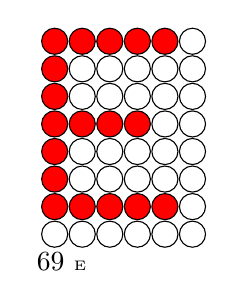
\begin{tikzpicture}[x=3.5mm,y=3.5mm]
\node [right] at (0,0) {69 {\tiny E}};
\node [circle, fill=red, draw=black, minimum size=3mm] at (1,8) {};
\node [circle, fill=red, draw=black, minimum size=3mm] at (2,8) {};
\node [circle, fill=red, draw=black, minimum size=3mm] at (3,8) {};
\node [circle, fill=red, draw=black, minimum size=3mm] at (4,8) {};
\node [circle, fill=red, draw=black, minimum size=3mm] at (5,8) {};
\node [circle, fill=none, draw=black, minimum size=3mm] at (6,8) {};
\node [circle, fill=red, draw=black, minimum size=3mm] at (1,7) {};
\node [circle, fill=none, draw=black, minimum size=3mm] at (2,7) {};
\node [circle, fill=none, draw=black, minimum size=3mm] at (3,7) {};
\node [circle, fill=none, draw=black, minimum size=3mm] at (4,7) {};
\node [circle, fill=none, draw=black, minimum size=3mm] at (5,7) {};
\node [circle, fill=none, draw=black, minimum size=3mm] at (6,7) {};
\node [circle, fill=red, draw=black, minimum size=3mm] at (1,6) {};
\node [circle, fill=none, draw=black, minimum size=3mm] at (2,6) {};
\node [circle, fill=none, draw=black, minimum size=3mm] at (3,6) {};
\node [circle, fill=none, draw=black, minimum size=3mm] at (4,6) {};
\node [circle, fill=none, draw=black, minimum size=3mm] at (5,6) {};
\node [circle, fill=none, draw=black, minimum size=3mm] at (6,6) {};
\node [circle, fill=red, draw=black, minimum size=3mm] at (1,5) {};
\node [circle, fill=red, draw=black, minimum size=3mm] at (2,5) {};
\node [circle, fill=red, draw=black, minimum size=3mm] at (3,5) {};
\node [circle, fill=red, draw=black, minimum size=3mm] at (4,5) {};
\node [circle, fill=none, draw=black, minimum size=3mm] at (5,5) {};
\node [circle, fill=none, draw=black, minimum size=3mm] at (6,5) {};
\node [circle, fill=red, draw=black, minimum size=3mm] at (1,4) {};
\node [circle, fill=none, draw=black, minimum size=3mm] at (2,4) {};
\node [circle, fill=none, draw=black, minimum size=3mm] at (3,4) {};
\node [circle, fill=none, draw=black, minimum size=3mm] at (4,4) {};
\node [circle, fill=none, draw=black, minimum size=3mm] at (5,4) {};
\node [circle, fill=none, draw=black, minimum size=3mm] at (6,4) {};
\node [circle, fill=red, draw=black, minimum size=3mm] at (1,3) {};
\node [circle, fill=none, draw=black, minimum size=3mm] at (2,3) {};
\node [circle, fill=none, draw=black, minimum size=3mm] at (3,3) {};
\node [circle, fill=none, draw=black, minimum size=3mm] at (4,3) {};
\node [circle, fill=none, draw=black, minimum size=3mm] at (5,3) {};
\node [circle, fill=none, draw=black, minimum size=3mm] at (6,3) {};
\node [circle, fill=red, draw=black, minimum size=3mm] at (1,2) {};
\node [circle, fill=red, draw=black, minimum size=3mm] at (2,2) {};
\node [circle, fill=red, draw=black, minimum size=3mm] at (3,2) {};
\node [circle, fill=red, draw=black, minimum size=3mm] at (4,2) {};
\node [circle, fill=red, draw=black, minimum size=3mm] at (5,2) {};
\node [circle, fill=none, draw=black, minimum size=3mm] at (6,2) {};
\node [circle, fill=none, draw=black, minimum size=3mm] at (1,1) {};
\node [circle, fill=none, draw=black, minimum size=3mm] at (2,1) {};
\node [circle, fill=none, draw=black, minimum size=3mm] at (3,1) {};
\node [circle, fill=none, draw=black, minimum size=3mm] at (4,1) {};
\node [circle, fill=none, draw=black, minimum size=3mm] at (5,1) {};
\node [circle, fill=none, draw=black, minimum size=3mm] at (6,1) {};
\end{tikzpicture}% font 0 codepoint 70 name F space 6 width 5 offset 170
~ 
\noindent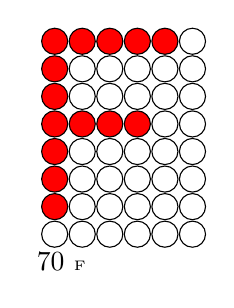
\begin{tikzpicture}[x=3.5mm,y=3.5mm]
\node [right] at (0,0) {70 {\tiny F}};
\node [circle, fill=red, draw=black, minimum size=3mm] at (1,8) {};
\node [circle, fill=red, draw=black, minimum size=3mm] at (2,8) {};
\node [circle, fill=red, draw=black, minimum size=3mm] at (3,8) {};
\node [circle, fill=red, draw=black, minimum size=3mm] at (4,8) {};
\node [circle, fill=red, draw=black, minimum size=3mm] at (5,8) {};
\node [circle, fill=none, draw=black, minimum size=3mm] at (6,8) {};
\node [circle, fill=red, draw=black, minimum size=3mm] at (1,7) {};
\node [circle, fill=none, draw=black, minimum size=3mm] at (2,7) {};
\node [circle, fill=none, draw=black, minimum size=3mm] at (3,7) {};
\node [circle, fill=none, draw=black, minimum size=3mm] at (4,7) {};
\node [circle, fill=none, draw=black, minimum size=3mm] at (5,7) {};
\node [circle, fill=none, draw=black, minimum size=3mm] at (6,7) {};
\node [circle, fill=red, draw=black, minimum size=3mm] at (1,6) {};
\node [circle, fill=none, draw=black, minimum size=3mm] at (2,6) {};
\node [circle, fill=none, draw=black, minimum size=3mm] at (3,6) {};
\node [circle, fill=none, draw=black, minimum size=3mm] at (4,6) {};
\node [circle, fill=none, draw=black, minimum size=3mm] at (5,6) {};
\node [circle, fill=none, draw=black, minimum size=3mm] at (6,6) {};
\node [circle, fill=red, draw=black, minimum size=3mm] at (1,5) {};
\node [circle, fill=red, draw=black, minimum size=3mm] at (2,5) {};
\node [circle, fill=red, draw=black, minimum size=3mm] at (3,5) {};
\node [circle, fill=red, draw=black, minimum size=3mm] at (4,5) {};
\node [circle, fill=none, draw=black, minimum size=3mm] at (5,5) {};
\node [circle, fill=none, draw=black, minimum size=3mm] at (6,5) {};
\node [circle, fill=red, draw=black, minimum size=3mm] at (1,4) {};
\node [circle, fill=none, draw=black, minimum size=3mm] at (2,4) {};
\node [circle, fill=none, draw=black, minimum size=3mm] at (3,4) {};
\node [circle, fill=none, draw=black, minimum size=3mm] at (4,4) {};
\node [circle, fill=none, draw=black, minimum size=3mm] at (5,4) {};
\node [circle, fill=none, draw=black, minimum size=3mm] at (6,4) {};
\node [circle, fill=red, draw=black, minimum size=3mm] at (1,3) {};
\node [circle, fill=none, draw=black, minimum size=3mm] at (2,3) {};
\node [circle, fill=none, draw=black, minimum size=3mm] at (3,3) {};
\node [circle, fill=none, draw=black, minimum size=3mm] at (4,3) {};
\node [circle, fill=none, draw=black, minimum size=3mm] at (5,3) {};
\node [circle, fill=none, draw=black, minimum size=3mm] at (6,3) {};
\node [circle, fill=red, draw=black, minimum size=3mm] at (1,2) {};
\node [circle, fill=none, draw=black, minimum size=3mm] at (2,2) {};
\node [circle, fill=none, draw=black, minimum size=3mm] at (3,2) {};
\node [circle, fill=none, draw=black, minimum size=3mm] at (4,2) {};
\node [circle, fill=none, draw=black, minimum size=3mm] at (5,2) {};
\node [circle, fill=none, draw=black, minimum size=3mm] at (6,2) {};
\node [circle, fill=none, draw=black, minimum size=3mm] at (1,1) {};
\node [circle, fill=none, draw=black, minimum size=3mm] at (2,1) {};
\node [circle, fill=none, draw=black, minimum size=3mm] at (3,1) {};
\node [circle, fill=none, draw=black, minimum size=3mm] at (4,1) {};
\node [circle, fill=none, draw=black, minimum size=3mm] at (5,1) {};
\node [circle, fill=none, draw=black, minimum size=3mm] at (6,1) {};
\end{tikzpicture}% font 0 codepoint 71 name G space 6 width 5 offset 175
~ 
\noindent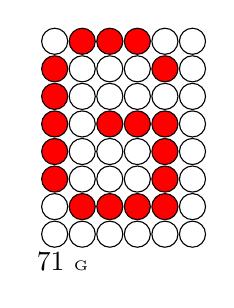
\begin{tikzpicture}[x=3.5mm,y=3.5mm]
\node [right] at (0,0) {71 {\tiny G}};
\node [circle, fill=none, draw=black, minimum size=3mm] at (1,8) {};
\node [circle, fill=red, draw=black, minimum size=3mm] at (2,8) {};
\node [circle, fill=red, draw=black, minimum size=3mm] at (3,8) {};
\node [circle, fill=red, draw=black, minimum size=3mm] at (4,8) {};
\node [circle, fill=none, draw=black, minimum size=3mm] at (5,8) {};
\node [circle, fill=none, draw=black, minimum size=3mm] at (6,8) {};
\node [circle, fill=red, draw=black, minimum size=3mm] at (1,7) {};
\node [circle, fill=none, draw=black, minimum size=3mm] at (2,7) {};
\node [circle, fill=none, draw=black, minimum size=3mm] at (3,7) {};
\node [circle, fill=none, draw=black, minimum size=3mm] at (4,7) {};
\node [circle, fill=red, draw=black, minimum size=3mm] at (5,7) {};
\node [circle, fill=none, draw=black, minimum size=3mm] at (6,7) {};
\node [circle, fill=red, draw=black, minimum size=3mm] at (1,6) {};
\node [circle, fill=none, draw=black, minimum size=3mm] at (2,6) {};
\node [circle, fill=none, draw=black, minimum size=3mm] at (3,6) {};
\node [circle, fill=none, draw=black, minimum size=3mm] at (4,6) {};
\node [circle, fill=none, draw=black, minimum size=3mm] at (5,6) {};
\node [circle, fill=none, draw=black, minimum size=3mm] at (6,6) {};
\node [circle, fill=red, draw=black, minimum size=3mm] at (1,5) {};
\node [circle, fill=none, draw=black, minimum size=3mm] at (2,5) {};
\node [circle, fill=red, draw=black, minimum size=3mm] at (3,5) {};
\node [circle, fill=red, draw=black, minimum size=3mm] at (4,5) {};
\node [circle, fill=red, draw=black, minimum size=3mm] at (5,5) {};
\node [circle, fill=none, draw=black, minimum size=3mm] at (6,5) {};
\node [circle, fill=red, draw=black, minimum size=3mm] at (1,4) {};
\node [circle, fill=none, draw=black, minimum size=3mm] at (2,4) {};
\node [circle, fill=none, draw=black, minimum size=3mm] at (3,4) {};
\node [circle, fill=none, draw=black, minimum size=3mm] at (4,4) {};
\node [circle, fill=red, draw=black, minimum size=3mm] at (5,4) {};
\node [circle, fill=none, draw=black, minimum size=3mm] at (6,4) {};
\node [circle, fill=red, draw=black, minimum size=3mm] at (1,3) {};
\node [circle, fill=none, draw=black, minimum size=3mm] at (2,3) {};
\node [circle, fill=none, draw=black, minimum size=3mm] at (3,3) {};
\node [circle, fill=none, draw=black, minimum size=3mm] at (4,3) {};
\node [circle, fill=red, draw=black, minimum size=3mm] at (5,3) {};
\node [circle, fill=none, draw=black, minimum size=3mm] at (6,3) {};
\node [circle, fill=none, draw=black, minimum size=3mm] at (1,2) {};
\node [circle, fill=red, draw=black, minimum size=3mm] at (2,2) {};
\node [circle, fill=red, draw=black, minimum size=3mm] at (3,2) {};
\node [circle, fill=red, draw=black, minimum size=3mm] at (4,2) {};
\node [circle, fill=red, draw=black, minimum size=3mm] at (5,2) {};
\node [circle, fill=none, draw=black, minimum size=3mm] at (6,2) {};
\node [circle, fill=none, draw=black, minimum size=3mm] at (1,1) {};
\node [circle, fill=none, draw=black, minimum size=3mm] at (2,1) {};
\node [circle, fill=none, draw=black, minimum size=3mm] at (3,1) {};
\node [circle, fill=none, draw=black, minimum size=3mm] at (4,1) {};
\node [circle, fill=none, draw=black, minimum size=3mm] at (5,1) {};
\node [circle, fill=none, draw=black, minimum size=3mm] at (6,1) {};
\end{tikzpicture}% font 0 codepoint 72 name H space 6 width 5 offset 180


\noindent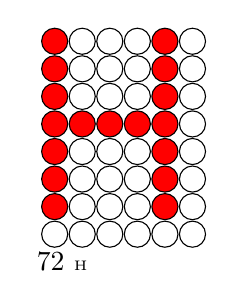
\begin{tikzpicture}[x=3.5mm,y=3.5mm]
\node [right] at (0,0) {72 {\tiny H}};
\node [circle, fill=red, draw=black, minimum size=3mm] at (1,8) {};
\node [circle, fill=none, draw=black, minimum size=3mm] at (2,8) {};
\node [circle, fill=none, draw=black, minimum size=3mm] at (3,8) {};
\node [circle, fill=none, draw=black, minimum size=3mm] at (4,8) {};
\node [circle, fill=red, draw=black, minimum size=3mm] at (5,8) {};
\node [circle, fill=none, draw=black, minimum size=3mm] at (6,8) {};
\node [circle, fill=red, draw=black, minimum size=3mm] at (1,7) {};
\node [circle, fill=none, draw=black, minimum size=3mm] at (2,7) {};
\node [circle, fill=none, draw=black, minimum size=3mm] at (3,7) {};
\node [circle, fill=none, draw=black, minimum size=3mm] at (4,7) {};
\node [circle, fill=red, draw=black, minimum size=3mm] at (5,7) {};
\node [circle, fill=none, draw=black, minimum size=3mm] at (6,7) {};
\node [circle, fill=red, draw=black, minimum size=3mm] at (1,6) {};
\node [circle, fill=none, draw=black, minimum size=3mm] at (2,6) {};
\node [circle, fill=none, draw=black, minimum size=3mm] at (3,6) {};
\node [circle, fill=none, draw=black, minimum size=3mm] at (4,6) {};
\node [circle, fill=red, draw=black, minimum size=3mm] at (5,6) {};
\node [circle, fill=none, draw=black, minimum size=3mm] at (6,6) {};
\node [circle, fill=red, draw=black, minimum size=3mm] at (1,5) {};
\node [circle, fill=red, draw=black, minimum size=3mm] at (2,5) {};
\node [circle, fill=red, draw=black, minimum size=3mm] at (3,5) {};
\node [circle, fill=red, draw=black, minimum size=3mm] at (4,5) {};
\node [circle, fill=red, draw=black, minimum size=3mm] at (5,5) {};
\node [circle, fill=none, draw=black, minimum size=3mm] at (6,5) {};
\node [circle, fill=red, draw=black, minimum size=3mm] at (1,4) {};
\node [circle, fill=none, draw=black, minimum size=3mm] at (2,4) {};
\node [circle, fill=none, draw=black, minimum size=3mm] at (3,4) {};
\node [circle, fill=none, draw=black, minimum size=3mm] at (4,4) {};
\node [circle, fill=red, draw=black, minimum size=3mm] at (5,4) {};
\node [circle, fill=none, draw=black, minimum size=3mm] at (6,4) {};
\node [circle, fill=red, draw=black, minimum size=3mm] at (1,3) {};
\node [circle, fill=none, draw=black, minimum size=3mm] at (2,3) {};
\node [circle, fill=none, draw=black, minimum size=3mm] at (3,3) {};
\node [circle, fill=none, draw=black, minimum size=3mm] at (4,3) {};
\node [circle, fill=red, draw=black, minimum size=3mm] at (5,3) {};
\node [circle, fill=none, draw=black, minimum size=3mm] at (6,3) {};
\node [circle, fill=red, draw=black, minimum size=3mm] at (1,2) {};
\node [circle, fill=none, draw=black, minimum size=3mm] at (2,2) {};
\node [circle, fill=none, draw=black, minimum size=3mm] at (3,2) {};
\node [circle, fill=none, draw=black, minimum size=3mm] at (4,2) {};
\node [circle, fill=red, draw=black, minimum size=3mm] at (5,2) {};
\node [circle, fill=none, draw=black, minimum size=3mm] at (6,2) {};
\node [circle, fill=none, draw=black, minimum size=3mm] at (1,1) {};
\node [circle, fill=none, draw=black, minimum size=3mm] at (2,1) {};
\node [circle, fill=none, draw=black, minimum size=3mm] at (3,1) {};
\node [circle, fill=none, draw=black, minimum size=3mm] at (4,1) {};
\node [circle, fill=none, draw=black, minimum size=3mm] at (5,1) {};
\node [circle, fill=none, draw=black, minimum size=3mm] at (6,1) {};
\end{tikzpicture}% font 0 codepoint 73 name I space 6 width 5 offset 185
~ 
\noindent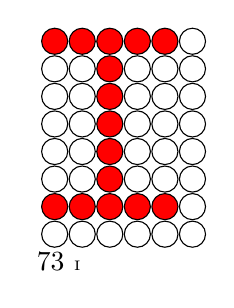
\begin{tikzpicture}[x=3.5mm,y=3.5mm]
\node [right] at (0,0) {73 {\tiny I}};
\node [circle, fill=red, draw=black, minimum size=3mm] at (1,8) {};
\node [circle, fill=red, draw=black, minimum size=3mm] at (2,8) {};
\node [circle, fill=red, draw=black, minimum size=3mm] at (3,8) {};
\node [circle, fill=red, draw=black, minimum size=3mm] at (4,8) {};
\node [circle, fill=red, draw=black, minimum size=3mm] at (5,8) {};
\node [circle, fill=none, draw=black, minimum size=3mm] at (6,8) {};
\node [circle, fill=none, draw=black, minimum size=3mm] at (1,7) {};
\node [circle, fill=none, draw=black, minimum size=3mm] at (2,7) {};
\node [circle, fill=red, draw=black, minimum size=3mm] at (3,7) {};
\node [circle, fill=none, draw=black, minimum size=3mm] at (4,7) {};
\node [circle, fill=none, draw=black, minimum size=3mm] at (5,7) {};
\node [circle, fill=none, draw=black, minimum size=3mm] at (6,7) {};
\node [circle, fill=none, draw=black, minimum size=3mm] at (1,6) {};
\node [circle, fill=none, draw=black, minimum size=3mm] at (2,6) {};
\node [circle, fill=red, draw=black, minimum size=3mm] at (3,6) {};
\node [circle, fill=none, draw=black, minimum size=3mm] at (4,6) {};
\node [circle, fill=none, draw=black, minimum size=3mm] at (5,6) {};
\node [circle, fill=none, draw=black, minimum size=3mm] at (6,6) {};
\node [circle, fill=none, draw=black, minimum size=3mm] at (1,5) {};
\node [circle, fill=none, draw=black, minimum size=3mm] at (2,5) {};
\node [circle, fill=red, draw=black, minimum size=3mm] at (3,5) {};
\node [circle, fill=none, draw=black, minimum size=3mm] at (4,5) {};
\node [circle, fill=none, draw=black, minimum size=3mm] at (5,5) {};
\node [circle, fill=none, draw=black, minimum size=3mm] at (6,5) {};
\node [circle, fill=none, draw=black, minimum size=3mm] at (1,4) {};
\node [circle, fill=none, draw=black, minimum size=3mm] at (2,4) {};
\node [circle, fill=red, draw=black, minimum size=3mm] at (3,4) {};
\node [circle, fill=none, draw=black, minimum size=3mm] at (4,4) {};
\node [circle, fill=none, draw=black, minimum size=3mm] at (5,4) {};
\node [circle, fill=none, draw=black, minimum size=3mm] at (6,4) {};
\node [circle, fill=none, draw=black, minimum size=3mm] at (1,3) {};
\node [circle, fill=none, draw=black, minimum size=3mm] at (2,3) {};
\node [circle, fill=red, draw=black, minimum size=3mm] at (3,3) {};
\node [circle, fill=none, draw=black, minimum size=3mm] at (4,3) {};
\node [circle, fill=none, draw=black, minimum size=3mm] at (5,3) {};
\node [circle, fill=none, draw=black, minimum size=3mm] at (6,3) {};
\node [circle, fill=red, draw=black, minimum size=3mm] at (1,2) {};
\node [circle, fill=red, draw=black, minimum size=3mm] at (2,2) {};
\node [circle, fill=red, draw=black, minimum size=3mm] at (3,2) {};
\node [circle, fill=red, draw=black, minimum size=3mm] at (4,2) {};
\node [circle, fill=red, draw=black, minimum size=3mm] at (5,2) {};
\node [circle, fill=none, draw=black, minimum size=3mm] at (6,2) {};
\node [circle, fill=none, draw=black, minimum size=3mm] at (1,1) {};
\node [circle, fill=none, draw=black, minimum size=3mm] at (2,1) {};
\node [circle, fill=none, draw=black, minimum size=3mm] at (3,1) {};
\node [circle, fill=none, draw=black, minimum size=3mm] at (4,1) {};
\node [circle, fill=none, draw=black, minimum size=3mm] at (5,1) {};
\node [circle, fill=none, draw=black, minimum size=3mm] at (6,1) {};
\end{tikzpicture}% font 0 codepoint 74 name J space 6 width 5 offset 190
~ 
\noindent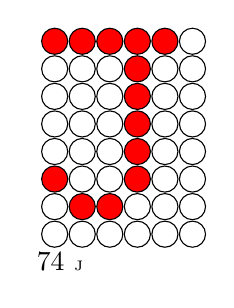
\begin{tikzpicture}[x=3.5mm,y=3.5mm]
\node [right] at (0,0) {74 {\tiny J}};
\node [circle, fill=red, draw=black, minimum size=3mm] at (1,8) {};
\node [circle, fill=red, draw=black, minimum size=3mm] at (2,8) {};
\node [circle, fill=red, draw=black, minimum size=3mm] at (3,8) {};
\node [circle, fill=red, draw=black, minimum size=3mm] at (4,8) {};
\node [circle, fill=red, draw=black, minimum size=3mm] at (5,8) {};
\node [circle, fill=none, draw=black, minimum size=3mm] at (6,8) {};
\node [circle, fill=none, draw=black, minimum size=3mm] at (1,7) {};
\node [circle, fill=none, draw=black, minimum size=3mm] at (2,7) {};
\node [circle, fill=none, draw=black, minimum size=3mm] at (3,7) {};
\node [circle, fill=red, draw=black, minimum size=3mm] at (4,7) {};
\node [circle, fill=none, draw=black, minimum size=3mm] at (5,7) {};
\node [circle, fill=none, draw=black, minimum size=3mm] at (6,7) {};
\node [circle, fill=none, draw=black, minimum size=3mm] at (1,6) {};
\node [circle, fill=none, draw=black, minimum size=3mm] at (2,6) {};
\node [circle, fill=none, draw=black, minimum size=3mm] at (3,6) {};
\node [circle, fill=red, draw=black, minimum size=3mm] at (4,6) {};
\node [circle, fill=none, draw=black, minimum size=3mm] at (5,6) {};
\node [circle, fill=none, draw=black, minimum size=3mm] at (6,6) {};
\node [circle, fill=none, draw=black, minimum size=3mm] at (1,5) {};
\node [circle, fill=none, draw=black, minimum size=3mm] at (2,5) {};
\node [circle, fill=none, draw=black, minimum size=3mm] at (3,5) {};
\node [circle, fill=red, draw=black, minimum size=3mm] at (4,5) {};
\node [circle, fill=none, draw=black, minimum size=3mm] at (5,5) {};
\node [circle, fill=none, draw=black, minimum size=3mm] at (6,5) {};
\node [circle, fill=none, draw=black, minimum size=3mm] at (1,4) {};
\node [circle, fill=none, draw=black, minimum size=3mm] at (2,4) {};
\node [circle, fill=none, draw=black, minimum size=3mm] at (3,4) {};
\node [circle, fill=red, draw=black, minimum size=3mm] at (4,4) {};
\node [circle, fill=none, draw=black, minimum size=3mm] at (5,4) {};
\node [circle, fill=none, draw=black, minimum size=3mm] at (6,4) {};
\node [circle, fill=red, draw=black, minimum size=3mm] at (1,3) {};
\node [circle, fill=none, draw=black, minimum size=3mm] at (2,3) {};
\node [circle, fill=none, draw=black, minimum size=3mm] at (3,3) {};
\node [circle, fill=red, draw=black, minimum size=3mm] at (4,3) {};
\node [circle, fill=none, draw=black, minimum size=3mm] at (5,3) {};
\node [circle, fill=none, draw=black, minimum size=3mm] at (6,3) {};
\node [circle, fill=none, draw=black, minimum size=3mm] at (1,2) {};
\node [circle, fill=red, draw=black, minimum size=3mm] at (2,2) {};
\node [circle, fill=red, draw=black, minimum size=3mm] at (3,2) {};
\node [circle, fill=none, draw=black, minimum size=3mm] at (4,2) {};
\node [circle, fill=none, draw=black, minimum size=3mm] at (5,2) {};
\node [circle, fill=none, draw=black, minimum size=3mm] at (6,2) {};
\node [circle, fill=none, draw=black, minimum size=3mm] at (1,1) {};
\node [circle, fill=none, draw=black, minimum size=3mm] at (2,1) {};
\node [circle, fill=none, draw=black, minimum size=3mm] at (3,1) {};
\node [circle, fill=none, draw=black, minimum size=3mm] at (4,1) {};
\node [circle, fill=none, draw=black, minimum size=3mm] at (5,1) {};
\node [circle, fill=none, draw=black, minimum size=3mm] at (6,1) {};
\end{tikzpicture}% font 0 codepoint 75 name K space 6 width 5 offset 195
~ 
\noindent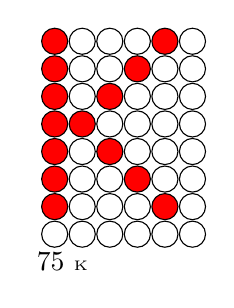
\begin{tikzpicture}[x=3.5mm,y=3.5mm]
\node [right] at (0,0) {75 {\tiny K}};
\node [circle, fill=red, draw=black, minimum size=3mm] at (1,8) {};
\node [circle, fill=none, draw=black, minimum size=3mm] at (2,8) {};
\node [circle, fill=none, draw=black, minimum size=3mm] at (3,8) {};
\node [circle, fill=none, draw=black, minimum size=3mm] at (4,8) {};
\node [circle, fill=red, draw=black, minimum size=3mm] at (5,8) {};
\node [circle, fill=none, draw=black, minimum size=3mm] at (6,8) {};
\node [circle, fill=red, draw=black, minimum size=3mm] at (1,7) {};
\node [circle, fill=none, draw=black, minimum size=3mm] at (2,7) {};
\node [circle, fill=none, draw=black, minimum size=3mm] at (3,7) {};
\node [circle, fill=red, draw=black, minimum size=3mm] at (4,7) {};
\node [circle, fill=none, draw=black, minimum size=3mm] at (5,7) {};
\node [circle, fill=none, draw=black, minimum size=3mm] at (6,7) {};
\node [circle, fill=red, draw=black, minimum size=3mm] at (1,6) {};
\node [circle, fill=none, draw=black, minimum size=3mm] at (2,6) {};
\node [circle, fill=red, draw=black, minimum size=3mm] at (3,6) {};
\node [circle, fill=none, draw=black, minimum size=3mm] at (4,6) {};
\node [circle, fill=none, draw=black, minimum size=3mm] at (5,6) {};
\node [circle, fill=none, draw=black, minimum size=3mm] at (6,6) {};
\node [circle, fill=red, draw=black, minimum size=3mm] at (1,5) {};
\node [circle, fill=red, draw=black, minimum size=3mm] at (2,5) {};
\node [circle, fill=none, draw=black, minimum size=3mm] at (3,5) {};
\node [circle, fill=none, draw=black, minimum size=3mm] at (4,5) {};
\node [circle, fill=none, draw=black, minimum size=3mm] at (5,5) {};
\node [circle, fill=none, draw=black, minimum size=3mm] at (6,5) {};
\node [circle, fill=red, draw=black, minimum size=3mm] at (1,4) {};
\node [circle, fill=none, draw=black, minimum size=3mm] at (2,4) {};
\node [circle, fill=red, draw=black, minimum size=3mm] at (3,4) {};
\node [circle, fill=none, draw=black, minimum size=3mm] at (4,4) {};
\node [circle, fill=none, draw=black, minimum size=3mm] at (5,4) {};
\node [circle, fill=none, draw=black, minimum size=3mm] at (6,4) {};
\node [circle, fill=red, draw=black, minimum size=3mm] at (1,3) {};
\node [circle, fill=none, draw=black, minimum size=3mm] at (2,3) {};
\node [circle, fill=none, draw=black, minimum size=3mm] at (3,3) {};
\node [circle, fill=red, draw=black, minimum size=3mm] at (4,3) {};
\node [circle, fill=none, draw=black, minimum size=3mm] at (5,3) {};
\node [circle, fill=none, draw=black, minimum size=3mm] at (6,3) {};
\node [circle, fill=red, draw=black, minimum size=3mm] at (1,2) {};
\node [circle, fill=none, draw=black, minimum size=3mm] at (2,2) {};
\node [circle, fill=none, draw=black, minimum size=3mm] at (3,2) {};
\node [circle, fill=none, draw=black, minimum size=3mm] at (4,2) {};
\node [circle, fill=red, draw=black, minimum size=3mm] at (5,2) {};
\node [circle, fill=none, draw=black, minimum size=3mm] at (6,2) {};
\node [circle, fill=none, draw=black, minimum size=3mm] at (1,1) {};
\node [circle, fill=none, draw=black, minimum size=3mm] at (2,1) {};
\node [circle, fill=none, draw=black, minimum size=3mm] at (3,1) {};
\node [circle, fill=none, draw=black, minimum size=3mm] at (4,1) {};
\node [circle, fill=none, draw=black, minimum size=3mm] at (5,1) {};
\node [circle, fill=none, draw=black, minimum size=3mm] at (6,1) {};
\end{tikzpicture}% font 0 codepoint 76 name L space 6 width 5 offset 200
~ 
\noindent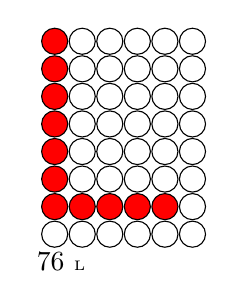
\begin{tikzpicture}[x=3.5mm,y=3.5mm]
\node [right] at (0,0) {76 {\tiny L}};
\node [circle, fill=red, draw=black, minimum size=3mm] at (1,8) {};
\node [circle, fill=none, draw=black, minimum size=3mm] at (2,8) {};
\node [circle, fill=none, draw=black, minimum size=3mm] at (3,8) {};
\node [circle, fill=none, draw=black, minimum size=3mm] at (4,8) {};
\node [circle, fill=none, draw=black, minimum size=3mm] at (5,8) {};
\node [circle, fill=none, draw=black, minimum size=3mm] at (6,8) {};
\node [circle, fill=red, draw=black, minimum size=3mm] at (1,7) {};
\node [circle, fill=none, draw=black, minimum size=3mm] at (2,7) {};
\node [circle, fill=none, draw=black, minimum size=3mm] at (3,7) {};
\node [circle, fill=none, draw=black, minimum size=3mm] at (4,7) {};
\node [circle, fill=none, draw=black, minimum size=3mm] at (5,7) {};
\node [circle, fill=none, draw=black, minimum size=3mm] at (6,7) {};
\node [circle, fill=red, draw=black, minimum size=3mm] at (1,6) {};
\node [circle, fill=none, draw=black, minimum size=3mm] at (2,6) {};
\node [circle, fill=none, draw=black, minimum size=3mm] at (3,6) {};
\node [circle, fill=none, draw=black, minimum size=3mm] at (4,6) {};
\node [circle, fill=none, draw=black, minimum size=3mm] at (5,6) {};
\node [circle, fill=none, draw=black, minimum size=3mm] at (6,6) {};
\node [circle, fill=red, draw=black, minimum size=3mm] at (1,5) {};
\node [circle, fill=none, draw=black, minimum size=3mm] at (2,5) {};
\node [circle, fill=none, draw=black, minimum size=3mm] at (3,5) {};
\node [circle, fill=none, draw=black, minimum size=3mm] at (4,5) {};
\node [circle, fill=none, draw=black, minimum size=3mm] at (5,5) {};
\node [circle, fill=none, draw=black, minimum size=3mm] at (6,5) {};
\node [circle, fill=red, draw=black, minimum size=3mm] at (1,4) {};
\node [circle, fill=none, draw=black, minimum size=3mm] at (2,4) {};
\node [circle, fill=none, draw=black, minimum size=3mm] at (3,4) {};
\node [circle, fill=none, draw=black, minimum size=3mm] at (4,4) {};
\node [circle, fill=none, draw=black, minimum size=3mm] at (5,4) {};
\node [circle, fill=none, draw=black, minimum size=3mm] at (6,4) {};
\node [circle, fill=red, draw=black, minimum size=3mm] at (1,3) {};
\node [circle, fill=none, draw=black, minimum size=3mm] at (2,3) {};
\node [circle, fill=none, draw=black, minimum size=3mm] at (3,3) {};
\node [circle, fill=none, draw=black, minimum size=3mm] at (4,3) {};
\node [circle, fill=none, draw=black, minimum size=3mm] at (5,3) {};
\node [circle, fill=none, draw=black, minimum size=3mm] at (6,3) {};
\node [circle, fill=red, draw=black, minimum size=3mm] at (1,2) {};
\node [circle, fill=red, draw=black, minimum size=3mm] at (2,2) {};
\node [circle, fill=red, draw=black, minimum size=3mm] at (3,2) {};
\node [circle, fill=red, draw=black, minimum size=3mm] at (4,2) {};
\node [circle, fill=red, draw=black, minimum size=3mm] at (5,2) {};
\node [circle, fill=none, draw=black, minimum size=3mm] at (6,2) {};
\node [circle, fill=none, draw=black, minimum size=3mm] at (1,1) {};
\node [circle, fill=none, draw=black, minimum size=3mm] at (2,1) {};
\node [circle, fill=none, draw=black, minimum size=3mm] at (3,1) {};
\node [circle, fill=none, draw=black, minimum size=3mm] at (4,1) {};
\node [circle, fill=none, draw=black, minimum size=3mm] at (5,1) {};
\node [circle, fill=none, draw=black, minimum size=3mm] at (6,1) {};
\end{tikzpicture}% font 0 codepoint 77 name M space 6 width 5 offset 205


\noindent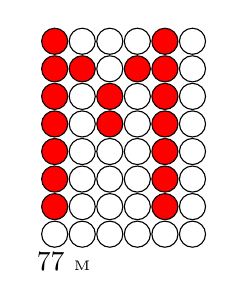
\begin{tikzpicture}[x=3.5mm,y=3.5mm]
\node [right] at (0,0) {77 {\tiny M}};
\node [circle, fill=red, draw=black, minimum size=3mm] at (1,8) {};
\node [circle, fill=none, draw=black, minimum size=3mm] at (2,8) {};
\node [circle, fill=none, draw=black, minimum size=3mm] at (3,8) {};
\node [circle, fill=none, draw=black, minimum size=3mm] at (4,8) {};
\node [circle, fill=red, draw=black, minimum size=3mm] at (5,8) {};
\node [circle, fill=none, draw=black, minimum size=3mm] at (6,8) {};
\node [circle, fill=red, draw=black, minimum size=3mm] at (1,7) {};
\node [circle, fill=red, draw=black, minimum size=3mm] at (2,7) {};
\node [circle, fill=none, draw=black, minimum size=3mm] at (3,7) {};
\node [circle, fill=red, draw=black, minimum size=3mm] at (4,7) {};
\node [circle, fill=red, draw=black, minimum size=3mm] at (5,7) {};
\node [circle, fill=none, draw=black, minimum size=3mm] at (6,7) {};
\node [circle, fill=red, draw=black, minimum size=3mm] at (1,6) {};
\node [circle, fill=none, draw=black, minimum size=3mm] at (2,6) {};
\node [circle, fill=red, draw=black, minimum size=3mm] at (3,6) {};
\node [circle, fill=none, draw=black, minimum size=3mm] at (4,6) {};
\node [circle, fill=red, draw=black, minimum size=3mm] at (5,6) {};
\node [circle, fill=none, draw=black, minimum size=3mm] at (6,6) {};
\node [circle, fill=red, draw=black, minimum size=3mm] at (1,5) {};
\node [circle, fill=none, draw=black, minimum size=3mm] at (2,5) {};
\node [circle, fill=red, draw=black, minimum size=3mm] at (3,5) {};
\node [circle, fill=none, draw=black, minimum size=3mm] at (4,5) {};
\node [circle, fill=red, draw=black, minimum size=3mm] at (5,5) {};
\node [circle, fill=none, draw=black, minimum size=3mm] at (6,5) {};
\node [circle, fill=red, draw=black, minimum size=3mm] at (1,4) {};
\node [circle, fill=none, draw=black, minimum size=3mm] at (2,4) {};
\node [circle, fill=none, draw=black, minimum size=3mm] at (3,4) {};
\node [circle, fill=none, draw=black, minimum size=3mm] at (4,4) {};
\node [circle, fill=red, draw=black, minimum size=3mm] at (5,4) {};
\node [circle, fill=none, draw=black, minimum size=3mm] at (6,4) {};
\node [circle, fill=red, draw=black, minimum size=3mm] at (1,3) {};
\node [circle, fill=none, draw=black, minimum size=3mm] at (2,3) {};
\node [circle, fill=none, draw=black, minimum size=3mm] at (3,3) {};
\node [circle, fill=none, draw=black, minimum size=3mm] at (4,3) {};
\node [circle, fill=red, draw=black, minimum size=3mm] at (5,3) {};
\node [circle, fill=none, draw=black, minimum size=3mm] at (6,3) {};
\node [circle, fill=red, draw=black, minimum size=3mm] at (1,2) {};
\node [circle, fill=none, draw=black, minimum size=3mm] at (2,2) {};
\node [circle, fill=none, draw=black, minimum size=3mm] at (3,2) {};
\node [circle, fill=none, draw=black, minimum size=3mm] at (4,2) {};
\node [circle, fill=red, draw=black, minimum size=3mm] at (5,2) {};
\node [circle, fill=none, draw=black, minimum size=3mm] at (6,2) {};
\node [circle, fill=none, draw=black, minimum size=3mm] at (1,1) {};
\node [circle, fill=none, draw=black, minimum size=3mm] at (2,1) {};
\node [circle, fill=none, draw=black, minimum size=3mm] at (3,1) {};
\node [circle, fill=none, draw=black, minimum size=3mm] at (4,1) {};
\node [circle, fill=none, draw=black, minimum size=3mm] at (5,1) {};
\node [circle, fill=none, draw=black, minimum size=3mm] at (6,1) {};
\end{tikzpicture}% font 0 codepoint 78 name N space 6 width 5 offset 210
~ 
\noindent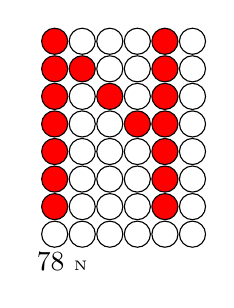
\begin{tikzpicture}[x=3.5mm,y=3.5mm]
\node [right] at (0,0) {78 {\tiny N}};
\node [circle, fill=red, draw=black, minimum size=3mm] at (1,8) {};
\node [circle, fill=none, draw=black, minimum size=3mm] at (2,8) {};
\node [circle, fill=none, draw=black, minimum size=3mm] at (3,8) {};
\node [circle, fill=none, draw=black, minimum size=3mm] at (4,8) {};
\node [circle, fill=red, draw=black, minimum size=3mm] at (5,8) {};
\node [circle, fill=none, draw=black, minimum size=3mm] at (6,8) {};
\node [circle, fill=red, draw=black, minimum size=3mm] at (1,7) {};
\node [circle, fill=red, draw=black, minimum size=3mm] at (2,7) {};
\node [circle, fill=none, draw=black, minimum size=3mm] at (3,7) {};
\node [circle, fill=none, draw=black, minimum size=3mm] at (4,7) {};
\node [circle, fill=red, draw=black, minimum size=3mm] at (5,7) {};
\node [circle, fill=none, draw=black, minimum size=3mm] at (6,7) {};
\node [circle, fill=red, draw=black, minimum size=3mm] at (1,6) {};
\node [circle, fill=none, draw=black, minimum size=3mm] at (2,6) {};
\node [circle, fill=red, draw=black, minimum size=3mm] at (3,6) {};
\node [circle, fill=none, draw=black, minimum size=3mm] at (4,6) {};
\node [circle, fill=red, draw=black, minimum size=3mm] at (5,6) {};
\node [circle, fill=none, draw=black, minimum size=3mm] at (6,6) {};
\node [circle, fill=red, draw=black, minimum size=3mm] at (1,5) {};
\node [circle, fill=none, draw=black, minimum size=3mm] at (2,5) {};
\node [circle, fill=none, draw=black, minimum size=3mm] at (3,5) {};
\node [circle, fill=red, draw=black, minimum size=3mm] at (4,5) {};
\node [circle, fill=red, draw=black, minimum size=3mm] at (5,5) {};
\node [circle, fill=none, draw=black, minimum size=3mm] at (6,5) {};
\node [circle, fill=red, draw=black, minimum size=3mm] at (1,4) {};
\node [circle, fill=none, draw=black, minimum size=3mm] at (2,4) {};
\node [circle, fill=none, draw=black, minimum size=3mm] at (3,4) {};
\node [circle, fill=none, draw=black, minimum size=3mm] at (4,4) {};
\node [circle, fill=red, draw=black, minimum size=3mm] at (5,4) {};
\node [circle, fill=none, draw=black, minimum size=3mm] at (6,4) {};
\node [circle, fill=red, draw=black, minimum size=3mm] at (1,3) {};
\node [circle, fill=none, draw=black, minimum size=3mm] at (2,3) {};
\node [circle, fill=none, draw=black, minimum size=3mm] at (3,3) {};
\node [circle, fill=none, draw=black, minimum size=3mm] at (4,3) {};
\node [circle, fill=red, draw=black, minimum size=3mm] at (5,3) {};
\node [circle, fill=none, draw=black, minimum size=3mm] at (6,3) {};
\node [circle, fill=red, draw=black, minimum size=3mm] at (1,2) {};
\node [circle, fill=none, draw=black, minimum size=3mm] at (2,2) {};
\node [circle, fill=none, draw=black, minimum size=3mm] at (3,2) {};
\node [circle, fill=none, draw=black, minimum size=3mm] at (4,2) {};
\node [circle, fill=red, draw=black, minimum size=3mm] at (5,2) {};
\node [circle, fill=none, draw=black, minimum size=3mm] at (6,2) {};
\node [circle, fill=none, draw=black, minimum size=3mm] at (1,1) {};
\node [circle, fill=none, draw=black, minimum size=3mm] at (2,1) {};
\node [circle, fill=none, draw=black, minimum size=3mm] at (3,1) {};
\node [circle, fill=none, draw=black, minimum size=3mm] at (4,1) {};
\node [circle, fill=none, draw=black, minimum size=3mm] at (5,1) {};
\node [circle, fill=none, draw=black, minimum size=3mm] at (6,1) {};
\end{tikzpicture}% font 0 codepoint 79 name O space 6 width 5 offset 215
~ 
\noindent\begin{tikzpicture}[x=3.5mm,y=3.5mm]
\node [right] at (0,0) {79 {\tiny O}};
\node [circle, fill=none, draw=black, minimum size=3mm] at (1,8) {};
\node [circle, fill=red, draw=black, minimum size=3mm] at (2,8) {};
\node [circle, fill=red, draw=black, minimum size=3mm] at (3,8) {};
\node [circle, fill=red, draw=black, minimum size=3mm] at (4,8) {};
\node [circle, fill=none, draw=black, minimum size=3mm] at (5,8) {};
\node [circle, fill=none, draw=black, minimum size=3mm] at (6,8) {};
\node [circle, fill=red, draw=black, minimum size=3mm] at (1,7) {};
\node [circle, fill=none, draw=black, minimum size=3mm] at (2,7) {};
\node [circle, fill=none, draw=black, minimum size=3mm] at (3,7) {};
\node [circle, fill=none, draw=black, minimum size=3mm] at (4,7) {};
\node [circle, fill=red, draw=black, minimum size=3mm] at (5,7) {};
\node [circle, fill=none, draw=black, minimum size=3mm] at (6,7) {};
\node [circle, fill=red, draw=black, minimum size=3mm] at (1,6) {};
\node [circle, fill=none, draw=black, minimum size=3mm] at (2,6) {};
\node [circle, fill=none, draw=black, minimum size=3mm] at (3,6) {};
\node [circle, fill=none, draw=black, minimum size=3mm] at (4,6) {};
\node [circle, fill=red, draw=black, minimum size=3mm] at (5,6) {};
\node [circle, fill=none, draw=black, minimum size=3mm] at (6,6) {};
\node [circle, fill=red, draw=black, minimum size=3mm] at (1,5) {};
\node [circle, fill=none, draw=black, minimum size=3mm] at (2,5) {};
\node [circle, fill=none, draw=black, minimum size=3mm] at (3,5) {};
\node [circle, fill=none, draw=black, minimum size=3mm] at (4,5) {};
\node [circle, fill=red, draw=black, minimum size=3mm] at (5,5) {};
\node [circle, fill=none, draw=black, minimum size=3mm] at (6,5) {};
\node [circle, fill=red, draw=black, minimum size=3mm] at (1,4) {};
\node [circle, fill=none, draw=black, minimum size=3mm] at (2,4) {};
\node [circle, fill=none, draw=black, minimum size=3mm] at (3,4) {};
\node [circle, fill=none, draw=black, minimum size=3mm] at (4,4) {};
\node [circle, fill=red, draw=black, minimum size=3mm] at (5,4) {};
\node [circle, fill=none, draw=black, minimum size=3mm] at (6,4) {};
\node [circle, fill=red, draw=black, minimum size=3mm] at (1,3) {};
\node [circle, fill=none, draw=black, minimum size=3mm] at (2,3) {};
\node [circle, fill=none, draw=black, minimum size=3mm] at (3,3) {};
\node [circle, fill=none, draw=black, minimum size=3mm] at (4,3) {};
\node [circle, fill=red, draw=black, minimum size=3mm] at (5,3) {};
\node [circle, fill=none, draw=black, minimum size=3mm] at (6,3) {};
\node [circle, fill=none, draw=black, minimum size=3mm] at (1,2) {};
\node [circle, fill=red, draw=black, minimum size=3mm] at (2,2) {};
\node [circle, fill=red, draw=black, minimum size=3mm] at (3,2) {};
\node [circle, fill=red, draw=black, minimum size=3mm] at (4,2) {};
\node [circle, fill=none, draw=black, minimum size=3mm] at (5,2) {};
\node [circle, fill=none, draw=black, minimum size=3mm] at (6,2) {};
\node [circle, fill=none, draw=black, minimum size=3mm] at (1,1) {};
\node [circle, fill=none, draw=black, minimum size=3mm] at (2,1) {};
\node [circle, fill=none, draw=black, minimum size=3mm] at (3,1) {};
\node [circle, fill=none, draw=black, minimum size=3mm] at (4,1) {};
\node [circle, fill=none, draw=black, minimum size=3mm] at (5,1) {};
\node [circle, fill=none, draw=black, minimum size=3mm] at (6,1) {};
\end{tikzpicture}% font 0 codepoint 80 name P space 6 width 5 offset 220
~ 
\noindent\begin{tikzpicture}[x=3.5mm,y=3.5mm]
\node [right] at (0,0) {80 {\tiny P}};
\node [circle, fill=red, draw=black, minimum size=3mm] at (1,8) {};
\node [circle, fill=red, draw=black, minimum size=3mm] at (2,8) {};
\node [circle, fill=red, draw=black, minimum size=3mm] at (3,8) {};
\node [circle, fill=red, draw=black, minimum size=3mm] at (4,8) {};
\node [circle, fill=none, draw=black, minimum size=3mm] at (5,8) {};
\node [circle, fill=none, draw=black, minimum size=3mm] at (6,8) {};
\node [circle, fill=red, draw=black, minimum size=3mm] at (1,7) {};
\node [circle, fill=none, draw=black, minimum size=3mm] at (2,7) {};
\node [circle, fill=none, draw=black, minimum size=3mm] at (3,7) {};
\node [circle, fill=none, draw=black, minimum size=3mm] at (4,7) {};
\node [circle, fill=red, draw=black, minimum size=3mm] at (5,7) {};
\node [circle, fill=none, draw=black, minimum size=3mm] at (6,7) {};
\node [circle, fill=red, draw=black, minimum size=3mm] at (1,6) {};
\node [circle, fill=none, draw=black, minimum size=3mm] at (2,6) {};
\node [circle, fill=none, draw=black, minimum size=3mm] at (3,6) {};
\node [circle, fill=none, draw=black, minimum size=3mm] at (4,6) {};
\node [circle, fill=red, draw=black, minimum size=3mm] at (5,6) {};
\node [circle, fill=none, draw=black, minimum size=3mm] at (6,6) {};
\node [circle, fill=red, draw=black, minimum size=3mm] at (1,5) {};
\node [circle, fill=red, draw=black, minimum size=3mm] at (2,5) {};
\node [circle, fill=red, draw=black, minimum size=3mm] at (3,5) {};
\node [circle, fill=red, draw=black, minimum size=3mm] at (4,5) {};
\node [circle, fill=none, draw=black, minimum size=3mm] at (5,5) {};
\node [circle, fill=none, draw=black, minimum size=3mm] at (6,5) {};
\node [circle, fill=red, draw=black, minimum size=3mm] at (1,4) {};
\node [circle, fill=none, draw=black, minimum size=3mm] at (2,4) {};
\node [circle, fill=none, draw=black, minimum size=3mm] at (3,4) {};
\node [circle, fill=none, draw=black, minimum size=3mm] at (4,4) {};
\node [circle, fill=none, draw=black, minimum size=3mm] at (5,4) {};
\node [circle, fill=none, draw=black, minimum size=3mm] at (6,4) {};
\node [circle, fill=red, draw=black, minimum size=3mm] at (1,3) {};
\node [circle, fill=none, draw=black, minimum size=3mm] at (2,3) {};
\node [circle, fill=none, draw=black, minimum size=3mm] at (3,3) {};
\node [circle, fill=none, draw=black, minimum size=3mm] at (4,3) {};
\node [circle, fill=none, draw=black, minimum size=3mm] at (5,3) {};
\node [circle, fill=none, draw=black, minimum size=3mm] at (6,3) {};
\node [circle, fill=red, draw=black, minimum size=3mm] at (1,2) {};
\node [circle, fill=none, draw=black, minimum size=3mm] at (2,2) {};
\node [circle, fill=none, draw=black, minimum size=3mm] at (3,2) {};
\node [circle, fill=none, draw=black, minimum size=3mm] at (4,2) {};
\node [circle, fill=none, draw=black, minimum size=3mm] at (5,2) {};
\node [circle, fill=none, draw=black, minimum size=3mm] at (6,2) {};
\node [circle, fill=none, draw=black, minimum size=3mm] at (1,1) {};
\node [circle, fill=none, draw=black, minimum size=3mm] at (2,1) {};
\node [circle, fill=none, draw=black, minimum size=3mm] at (3,1) {};
\node [circle, fill=none, draw=black, minimum size=3mm] at (4,1) {};
\node [circle, fill=none, draw=black, minimum size=3mm] at (5,1) {};
\node [circle, fill=none, draw=black, minimum size=3mm] at (6,1) {};
\end{tikzpicture}% font 0 codepoint 81 name Q space 6 width 5 offset 225
~ 
\noindent\begin{tikzpicture}[x=3.5mm,y=3.5mm]
\node [right] at (0,0) {81 {\tiny Q}};
\node [circle, fill=none, draw=black, minimum size=3mm] at (1,8) {};
\node [circle, fill=red, draw=black, minimum size=3mm] at (2,8) {};
\node [circle, fill=red, draw=black, minimum size=3mm] at (3,8) {};
\node [circle, fill=red, draw=black, minimum size=3mm] at (4,8) {};
\node [circle, fill=none, draw=black, minimum size=3mm] at (5,8) {};
\node [circle, fill=none, draw=black, minimum size=3mm] at (6,8) {};
\node [circle, fill=red, draw=black, minimum size=3mm] at (1,7) {};
\node [circle, fill=none, draw=black, minimum size=3mm] at (2,7) {};
\node [circle, fill=none, draw=black, minimum size=3mm] at (3,7) {};
\node [circle, fill=none, draw=black, minimum size=3mm] at (4,7) {};
\node [circle, fill=red, draw=black, minimum size=3mm] at (5,7) {};
\node [circle, fill=none, draw=black, minimum size=3mm] at (6,7) {};
\node [circle, fill=red, draw=black, minimum size=3mm] at (1,6) {};
\node [circle, fill=none, draw=black, minimum size=3mm] at (2,6) {};
\node [circle, fill=none, draw=black, minimum size=3mm] at (3,6) {};
\node [circle, fill=none, draw=black, minimum size=3mm] at (4,6) {};
\node [circle, fill=red, draw=black, minimum size=3mm] at (5,6) {};
\node [circle, fill=none, draw=black, minimum size=3mm] at (6,6) {};
\node [circle, fill=red, draw=black, minimum size=3mm] at (1,5) {};
\node [circle, fill=none, draw=black, minimum size=3mm] at (2,5) {};
\node [circle, fill=none, draw=black, minimum size=3mm] at (3,5) {};
\node [circle, fill=none, draw=black, minimum size=3mm] at (4,5) {};
\node [circle, fill=red, draw=black, minimum size=3mm] at (5,5) {};
\node [circle, fill=none, draw=black, minimum size=3mm] at (6,5) {};
\node [circle, fill=red, draw=black, minimum size=3mm] at (1,4) {};
\node [circle, fill=none, draw=black, minimum size=3mm] at (2,4) {};
\node [circle, fill=red, draw=black, minimum size=3mm] at (3,4) {};
\node [circle, fill=none, draw=black, minimum size=3mm] at (4,4) {};
\node [circle, fill=red, draw=black, minimum size=3mm] at (5,4) {};
\node [circle, fill=none, draw=black, minimum size=3mm] at (6,4) {};
\node [circle, fill=red, draw=black, minimum size=3mm] at (1,3) {};
\node [circle, fill=none, draw=black, minimum size=3mm] at (2,3) {};
\node [circle, fill=none, draw=black, minimum size=3mm] at (3,3) {};
\node [circle, fill=red, draw=black, minimum size=3mm] at (4,3) {};
\node [circle, fill=red, draw=black, minimum size=3mm] at (5,3) {};
\node [circle, fill=none, draw=black, minimum size=3mm] at (6,3) {};
\node [circle, fill=none, draw=black, minimum size=3mm] at (1,2) {};
\node [circle, fill=red, draw=black, minimum size=3mm] at (2,2) {};
\node [circle, fill=red, draw=black, minimum size=3mm] at (3,2) {};
\node [circle, fill=red, draw=black, minimum size=3mm] at (4,2) {};
\node [circle, fill=red, draw=black, minimum size=3mm] at (5,2) {};
\node [circle, fill=none, draw=black, minimum size=3mm] at (6,2) {};
\node [circle, fill=none, draw=black, minimum size=3mm] at (1,1) {};
\node [circle, fill=none, draw=black, minimum size=3mm] at (2,1) {};
\node [circle, fill=none, draw=black, minimum size=3mm] at (3,1) {};
\node [circle, fill=none, draw=black, minimum size=3mm] at (4,1) {};
\node [circle, fill=none, draw=black, minimum size=3mm] at (5,1) {};
\node [circle, fill=none, draw=black, minimum size=3mm] at (6,1) {};
\end{tikzpicture}% font 0 codepoint 82 name R space 6 width 5 offset 230


\noindent\begin{tikzpicture}[x=3.5mm,y=3.5mm]
\node [right] at (0,0) {82 {\tiny R}};
\node [circle, fill=red, draw=black, minimum size=3mm] at (1,8) {};
\node [circle, fill=red, draw=black, minimum size=3mm] at (2,8) {};
\node [circle, fill=red, draw=black, minimum size=3mm] at (3,8) {};
\node [circle, fill=red, draw=black, minimum size=3mm] at (4,8) {};
\node [circle, fill=none, draw=black, minimum size=3mm] at (5,8) {};
\node [circle, fill=none, draw=black, minimum size=3mm] at (6,8) {};
\node [circle, fill=red, draw=black, minimum size=3mm] at (1,7) {};
\node [circle, fill=none, draw=black, minimum size=3mm] at (2,7) {};
\node [circle, fill=none, draw=black, minimum size=3mm] at (3,7) {};
\node [circle, fill=none, draw=black, minimum size=3mm] at (4,7) {};
\node [circle, fill=red, draw=black, minimum size=3mm] at (5,7) {};
\node [circle, fill=none, draw=black, minimum size=3mm] at (6,7) {};
\node [circle, fill=red, draw=black, minimum size=3mm] at (1,6) {};
\node [circle, fill=none, draw=black, minimum size=3mm] at (2,6) {};
\node [circle, fill=none, draw=black, minimum size=3mm] at (3,6) {};
\node [circle, fill=none, draw=black, minimum size=3mm] at (4,6) {};
\node [circle, fill=red, draw=black, minimum size=3mm] at (5,6) {};
\node [circle, fill=none, draw=black, minimum size=3mm] at (6,6) {};
\node [circle, fill=red, draw=black, minimum size=3mm] at (1,5) {};
\node [circle, fill=red, draw=black, minimum size=3mm] at (2,5) {};
\node [circle, fill=red, draw=black, minimum size=3mm] at (3,5) {};
\node [circle, fill=red, draw=black, minimum size=3mm] at (4,5) {};
\node [circle, fill=none, draw=black, minimum size=3mm] at (5,5) {};
\node [circle, fill=none, draw=black, minimum size=3mm] at (6,5) {};
\node [circle, fill=red, draw=black, minimum size=3mm] at (1,4) {};
\node [circle, fill=none, draw=black, minimum size=3mm] at (2,4) {};
\node [circle, fill=red, draw=black, minimum size=3mm] at (3,4) {};
\node [circle, fill=none, draw=black, minimum size=3mm] at (4,4) {};
\node [circle, fill=none, draw=black, minimum size=3mm] at (5,4) {};
\node [circle, fill=none, draw=black, minimum size=3mm] at (6,4) {};
\node [circle, fill=red, draw=black, minimum size=3mm] at (1,3) {};
\node [circle, fill=none, draw=black, minimum size=3mm] at (2,3) {};
\node [circle, fill=none, draw=black, minimum size=3mm] at (3,3) {};
\node [circle, fill=red, draw=black, minimum size=3mm] at (4,3) {};
\node [circle, fill=none, draw=black, minimum size=3mm] at (5,3) {};
\node [circle, fill=none, draw=black, minimum size=3mm] at (6,3) {};
\node [circle, fill=red, draw=black, minimum size=3mm] at (1,2) {};
\node [circle, fill=none, draw=black, minimum size=3mm] at (2,2) {};
\node [circle, fill=none, draw=black, minimum size=3mm] at (3,2) {};
\node [circle, fill=none, draw=black, minimum size=3mm] at (4,2) {};
\node [circle, fill=red, draw=black, minimum size=3mm] at (5,2) {};
\node [circle, fill=none, draw=black, minimum size=3mm] at (6,2) {};
\node [circle, fill=none, draw=black, minimum size=3mm] at (1,1) {};
\node [circle, fill=none, draw=black, minimum size=3mm] at (2,1) {};
\node [circle, fill=none, draw=black, minimum size=3mm] at (3,1) {};
\node [circle, fill=none, draw=black, minimum size=3mm] at (4,1) {};
\node [circle, fill=none, draw=black, minimum size=3mm] at (5,1) {};
\node [circle, fill=none, draw=black, minimum size=3mm] at (6,1) {};
\end{tikzpicture}% font 0 codepoint 83 name S space 6 width 5 offset 235
~ 
\noindent\begin{tikzpicture}[x=3.5mm,y=3.5mm]
\node [right] at (0,0) {83 {\tiny S}};
\node [circle, fill=none, draw=black, minimum size=3mm] at (1,8) {};
\node [circle, fill=red, draw=black, minimum size=3mm] at (2,8) {};
\node [circle, fill=red, draw=black, minimum size=3mm] at (3,8) {};
\node [circle, fill=red, draw=black, minimum size=3mm] at (4,8) {};
\node [circle, fill=none, draw=black, minimum size=3mm] at (5,8) {};
\node [circle, fill=none, draw=black, minimum size=3mm] at (6,8) {};
\node [circle, fill=red, draw=black, minimum size=3mm] at (1,7) {};
\node [circle, fill=none, draw=black, minimum size=3mm] at (2,7) {};
\node [circle, fill=none, draw=black, minimum size=3mm] at (3,7) {};
\node [circle, fill=none, draw=black, minimum size=3mm] at (4,7) {};
\node [circle, fill=red, draw=black, minimum size=3mm] at (5,7) {};
\node [circle, fill=none, draw=black, minimum size=3mm] at (6,7) {};
\node [circle, fill=red, draw=black, minimum size=3mm] at (1,6) {};
\node [circle, fill=none, draw=black, minimum size=3mm] at (2,6) {};
\node [circle, fill=none, draw=black, minimum size=3mm] at (3,6) {};
\node [circle, fill=none, draw=black, minimum size=3mm] at (4,6) {};
\node [circle, fill=none, draw=black, minimum size=3mm] at (5,6) {};
\node [circle, fill=none, draw=black, minimum size=3mm] at (6,6) {};
\node [circle, fill=none, draw=black, minimum size=3mm] at (1,5) {};
\node [circle, fill=red, draw=black, minimum size=3mm] at (2,5) {};
\node [circle, fill=red, draw=black, minimum size=3mm] at (3,5) {};
\node [circle, fill=red, draw=black, minimum size=3mm] at (4,5) {};
\node [circle, fill=none, draw=black, minimum size=3mm] at (5,5) {};
\node [circle, fill=none, draw=black, minimum size=3mm] at (6,5) {};
\node [circle, fill=none, draw=black, minimum size=3mm] at (1,4) {};
\node [circle, fill=none, draw=black, minimum size=3mm] at (2,4) {};
\node [circle, fill=none, draw=black, minimum size=3mm] at (3,4) {};
\node [circle, fill=none, draw=black, minimum size=3mm] at (4,4) {};
\node [circle, fill=red, draw=black, minimum size=3mm] at (5,4) {};
\node [circle, fill=none, draw=black, minimum size=3mm] at (6,4) {};
\node [circle, fill=red, draw=black, minimum size=3mm] at (1,3) {};
\node [circle, fill=none, draw=black, minimum size=3mm] at (2,3) {};
\node [circle, fill=none, draw=black, minimum size=3mm] at (3,3) {};
\node [circle, fill=none, draw=black, minimum size=3mm] at (4,3) {};
\node [circle, fill=red, draw=black, minimum size=3mm] at (5,3) {};
\node [circle, fill=none, draw=black, minimum size=3mm] at (6,3) {};
\node [circle, fill=none, draw=black, minimum size=3mm] at (1,2) {};
\node [circle, fill=red, draw=black, minimum size=3mm] at (2,2) {};
\node [circle, fill=red, draw=black, minimum size=3mm] at (3,2) {};
\node [circle, fill=red, draw=black, minimum size=3mm] at (4,2) {};
\node [circle, fill=none, draw=black, minimum size=3mm] at (5,2) {};
\node [circle, fill=none, draw=black, minimum size=3mm] at (6,2) {};
\node [circle, fill=none, draw=black, minimum size=3mm] at (1,1) {};
\node [circle, fill=none, draw=black, minimum size=3mm] at (2,1) {};
\node [circle, fill=none, draw=black, minimum size=3mm] at (3,1) {};
\node [circle, fill=none, draw=black, minimum size=3mm] at (4,1) {};
\node [circle, fill=none, draw=black, minimum size=3mm] at (5,1) {};
\node [circle, fill=none, draw=black, minimum size=3mm] at (6,1) {};
\end{tikzpicture}% font 0 codepoint 84 name T space 6 width 5 offset 240
~ 
\noindent\begin{tikzpicture}[x=3.5mm,y=3.5mm]
\node [right] at (0,0) {84 {\tiny T}};
\node [circle, fill=red, draw=black, minimum size=3mm] at (1,8) {};
\node [circle, fill=red, draw=black, minimum size=3mm] at (2,8) {};
\node [circle, fill=red, draw=black, minimum size=3mm] at (3,8) {};
\node [circle, fill=red, draw=black, minimum size=3mm] at (4,8) {};
\node [circle, fill=red, draw=black, minimum size=3mm] at (5,8) {};
\node [circle, fill=none, draw=black, minimum size=3mm] at (6,8) {};
\node [circle, fill=none, draw=black, minimum size=3mm] at (1,7) {};
\node [circle, fill=none, draw=black, minimum size=3mm] at (2,7) {};
\node [circle, fill=red, draw=black, minimum size=3mm] at (3,7) {};
\node [circle, fill=none, draw=black, minimum size=3mm] at (4,7) {};
\node [circle, fill=none, draw=black, minimum size=3mm] at (5,7) {};
\node [circle, fill=none, draw=black, minimum size=3mm] at (6,7) {};
\node [circle, fill=none, draw=black, minimum size=3mm] at (1,6) {};
\node [circle, fill=none, draw=black, minimum size=3mm] at (2,6) {};
\node [circle, fill=red, draw=black, minimum size=3mm] at (3,6) {};
\node [circle, fill=none, draw=black, minimum size=3mm] at (4,6) {};
\node [circle, fill=none, draw=black, minimum size=3mm] at (5,6) {};
\node [circle, fill=none, draw=black, minimum size=3mm] at (6,6) {};
\node [circle, fill=none, draw=black, minimum size=3mm] at (1,5) {};
\node [circle, fill=none, draw=black, minimum size=3mm] at (2,5) {};
\node [circle, fill=red, draw=black, minimum size=3mm] at (3,5) {};
\node [circle, fill=none, draw=black, minimum size=3mm] at (4,5) {};
\node [circle, fill=none, draw=black, minimum size=3mm] at (5,5) {};
\node [circle, fill=none, draw=black, minimum size=3mm] at (6,5) {};
\node [circle, fill=none, draw=black, minimum size=3mm] at (1,4) {};
\node [circle, fill=none, draw=black, minimum size=3mm] at (2,4) {};
\node [circle, fill=red, draw=black, minimum size=3mm] at (3,4) {};
\node [circle, fill=none, draw=black, minimum size=3mm] at (4,4) {};
\node [circle, fill=none, draw=black, minimum size=3mm] at (5,4) {};
\node [circle, fill=none, draw=black, minimum size=3mm] at (6,4) {};
\node [circle, fill=none, draw=black, minimum size=3mm] at (1,3) {};
\node [circle, fill=none, draw=black, minimum size=3mm] at (2,3) {};
\node [circle, fill=red, draw=black, minimum size=3mm] at (3,3) {};
\node [circle, fill=none, draw=black, minimum size=3mm] at (4,3) {};
\node [circle, fill=none, draw=black, minimum size=3mm] at (5,3) {};
\node [circle, fill=none, draw=black, minimum size=3mm] at (6,3) {};
\node [circle, fill=none, draw=black, minimum size=3mm] at (1,2) {};
\node [circle, fill=none, draw=black, minimum size=3mm] at (2,2) {};
\node [circle, fill=red, draw=black, minimum size=3mm] at (3,2) {};
\node [circle, fill=none, draw=black, minimum size=3mm] at (4,2) {};
\node [circle, fill=none, draw=black, minimum size=3mm] at (5,2) {};
\node [circle, fill=none, draw=black, minimum size=3mm] at (6,2) {};
\node [circle, fill=none, draw=black, minimum size=3mm] at (1,1) {};
\node [circle, fill=none, draw=black, minimum size=3mm] at (2,1) {};
\node [circle, fill=none, draw=black, minimum size=3mm] at (3,1) {};
\node [circle, fill=none, draw=black, minimum size=3mm] at (4,1) {};
\node [circle, fill=none, draw=black, minimum size=3mm] at (5,1) {};
\node [circle, fill=none, draw=black, minimum size=3mm] at (6,1) {};
\end{tikzpicture}% font 0 codepoint 85 name U space 6 width 5 offset 245
~ 
\noindent\begin{tikzpicture}[x=3.5mm,y=3.5mm]
\node [right] at (0,0) {85 {\tiny U}};
\node [circle, fill=red, draw=black, minimum size=3mm] at (1,8) {};
\node [circle, fill=none, draw=black, minimum size=3mm] at (2,8) {};
\node [circle, fill=none, draw=black, minimum size=3mm] at (3,8) {};
\node [circle, fill=none, draw=black, minimum size=3mm] at (4,8) {};
\node [circle, fill=red, draw=black, minimum size=3mm] at (5,8) {};
\node [circle, fill=none, draw=black, minimum size=3mm] at (6,8) {};
\node [circle, fill=red, draw=black, minimum size=3mm] at (1,7) {};
\node [circle, fill=none, draw=black, minimum size=3mm] at (2,7) {};
\node [circle, fill=none, draw=black, minimum size=3mm] at (3,7) {};
\node [circle, fill=none, draw=black, minimum size=3mm] at (4,7) {};
\node [circle, fill=red, draw=black, minimum size=3mm] at (5,7) {};
\node [circle, fill=none, draw=black, minimum size=3mm] at (6,7) {};
\node [circle, fill=red, draw=black, minimum size=3mm] at (1,6) {};
\node [circle, fill=none, draw=black, minimum size=3mm] at (2,6) {};
\node [circle, fill=none, draw=black, minimum size=3mm] at (3,6) {};
\node [circle, fill=none, draw=black, minimum size=3mm] at (4,6) {};
\node [circle, fill=red, draw=black, minimum size=3mm] at (5,6) {};
\node [circle, fill=none, draw=black, minimum size=3mm] at (6,6) {};
\node [circle, fill=red, draw=black, minimum size=3mm] at (1,5) {};
\node [circle, fill=none, draw=black, minimum size=3mm] at (2,5) {};
\node [circle, fill=none, draw=black, minimum size=3mm] at (3,5) {};
\node [circle, fill=none, draw=black, minimum size=3mm] at (4,5) {};
\node [circle, fill=red, draw=black, minimum size=3mm] at (5,5) {};
\node [circle, fill=none, draw=black, minimum size=3mm] at (6,5) {};
\node [circle, fill=red, draw=black, minimum size=3mm] at (1,4) {};
\node [circle, fill=none, draw=black, minimum size=3mm] at (2,4) {};
\node [circle, fill=none, draw=black, minimum size=3mm] at (3,4) {};
\node [circle, fill=none, draw=black, minimum size=3mm] at (4,4) {};
\node [circle, fill=red, draw=black, minimum size=3mm] at (5,4) {};
\node [circle, fill=none, draw=black, minimum size=3mm] at (6,4) {};
\node [circle, fill=red, draw=black, minimum size=3mm] at (1,3) {};
\node [circle, fill=none, draw=black, minimum size=3mm] at (2,3) {};
\node [circle, fill=none, draw=black, minimum size=3mm] at (3,3) {};
\node [circle, fill=none, draw=black, minimum size=3mm] at (4,3) {};
\node [circle, fill=red, draw=black, minimum size=3mm] at (5,3) {};
\node [circle, fill=none, draw=black, minimum size=3mm] at (6,3) {};
\node [circle, fill=none, draw=black, minimum size=3mm] at (1,2) {};
\node [circle, fill=red, draw=black, minimum size=3mm] at (2,2) {};
\node [circle, fill=red, draw=black, minimum size=3mm] at (3,2) {};
\node [circle, fill=red, draw=black, minimum size=3mm] at (4,2) {};
\node [circle, fill=none, draw=black, minimum size=3mm] at (5,2) {};
\node [circle, fill=none, draw=black, minimum size=3mm] at (6,2) {};
\node [circle, fill=none, draw=black, minimum size=3mm] at (1,1) {};
\node [circle, fill=none, draw=black, minimum size=3mm] at (2,1) {};
\node [circle, fill=none, draw=black, minimum size=3mm] at (3,1) {};
\node [circle, fill=none, draw=black, minimum size=3mm] at (4,1) {};
\node [circle, fill=none, draw=black, minimum size=3mm] at (5,1) {};
\node [circle, fill=none, draw=black, minimum size=3mm] at (6,1) {};
\end{tikzpicture}% font 0 codepoint 86 name V space 6 width 5 offset 250
~ 
\noindent\begin{tikzpicture}[x=3.5mm,y=3.5mm]
\node [right] at (0,0) {86 {\tiny V}};
\node [circle, fill=red, draw=black, minimum size=3mm] at (1,8) {};
\node [circle, fill=none, draw=black, minimum size=3mm] at (2,8) {};
\node [circle, fill=none, draw=black, minimum size=3mm] at (3,8) {};
\node [circle, fill=none, draw=black, minimum size=3mm] at (4,8) {};
\node [circle, fill=red, draw=black, minimum size=3mm] at (5,8) {};
\node [circle, fill=none, draw=black, minimum size=3mm] at (6,8) {};
\node [circle, fill=red, draw=black, minimum size=3mm] at (1,7) {};
\node [circle, fill=none, draw=black, minimum size=3mm] at (2,7) {};
\node [circle, fill=none, draw=black, minimum size=3mm] at (3,7) {};
\node [circle, fill=none, draw=black, minimum size=3mm] at (4,7) {};
\node [circle, fill=red, draw=black, minimum size=3mm] at (5,7) {};
\node [circle, fill=none, draw=black, minimum size=3mm] at (6,7) {};
\node [circle, fill=red, draw=black, minimum size=3mm] at (1,6) {};
\node [circle, fill=none, draw=black, minimum size=3mm] at (2,6) {};
\node [circle, fill=none, draw=black, minimum size=3mm] at (3,6) {};
\node [circle, fill=none, draw=black, minimum size=3mm] at (4,6) {};
\node [circle, fill=red, draw=black, minimum size=3mm] at (5,6) {};
\node [circle, fill=none, draw=black, minimum size=3mm] at (6,6) {};
\node [circle, fill=red, draw=black, minimum size=3mm] at (1,5) {};
\node [circle, fill=none, draw=black, minimum size=3mm] at (2,5) {};
\node [circle, fill=none, draw=black, minimum size=3mm] at (3,5) {};
\node [circle, fill=none, draw=black, minimum size=3mm] at (4,5) {};
\node [circle, fill=red, draw=black, minimum size=3mm] at (5,5) {};
\node [circle, fill=none, draw=black, minimum size=3mm] at (6,5) {};
\node [circle, fill=none, draw=black, minimum size=3mm] at (1,4) {};
\node [circle, fill=red, draw=black, minimum size=3mm] at (2,4) {};
\node [circle, fill=none, draw=black, minimum size=3mm] at (3,4) {};
\node [circle, fill=red, draw=black, minimum size=3mm] at (4,4) {};
\node [circle, fill=none, draw=black, minimum size=3mm] at (5,4) {};
\node [circle, fill=none, draw=black, minimum size=3mm] at (6,4) {};
\node [circle, fill=none, draw=black, minimum size=3mm] at (1,3) {};
\node [circle, fill=red, draw=black, minimum size=3mm] at (2,3) {};
\node [circle, fill=none, draw=black, minimum size=3mm] at (3,3) {};
\node [circle, fill=red, draw=black, minimum size=3mm] at (4,3) {};
\node [circle, fill=none, draw=black, minimum size=3mm] at (5,3) {};
\node [circle, fill=none, draw=black, minimum size=3mm] at (6,3) {};
\node [circle, fill=none, draw=black, minimum size=3mm] at (1,2) {};
\node [circle, fill=none, draw=black, minimum size=3mm] at (2,2) {};
\node [circle, fill=red, draw=black, minimum size=3mm] at (3,2) {};
\node [circle, fill=none, draw=black, minimum size=3mm] at (4,2) {};
\node [circle, fill=none, draw=black, minimum size=3mm] at (5,2) {};
\node [circle, fill=none, draw=black, minimum size=3mm] at (6,2) {};
\node [circle, fill=none, draw=black, minimum size=3mm] at (1,1) {};
\node [circle, fill=none, draw=black, minimum size=3mm] at (2,1) {};
\node [circle, fill=none, draw=black, minimum size=3mm] at (3,1) {};
\node [circle, fill=none, draw=black, minimum size=3mm] at (4,1) {};
\node [circle, fill=none, draw=black, minimum size=3mm] at (5,1) {};
\node [circle, fill=none, draw=black, minimum size=3mm] at (6,1) {};
\end{tikzpicture}% font 0 codepoint 87 name W space 6 width 5 offset 255


\noindent\begin{tikzpicture}[x=3.5mm,y=3.5mm]
\node [right] at (0,0) {87 {\tiny W}};
\node [circle, fill=red, draw=black, minimum size=3mm] at (1,8) {};
\node [circle, fill=none, draw=black, minimum size=3mm] at (2,8) {};
\node [circle, fill=none, draw=black, minimum size=3mm] at (3,8) {};
\node [circle, fill=none, draw=black, minimum size=3mm] at (4,8) {};
\node [circle, fill=red, draw=black, minimum size=3mm] at (5,8) {};
\node [circle, fill=none, draw=black, minimum size=3mm] at (6,8) {};
\node [circle, fill=red, draw=black, minimum size=3mm] at (1,7) {};
\node [circle, fill=none, draw=black, minimum size=3mm] at (2,7) {};
\node [circle, fill=none, draw=black, minimum size=3mm] at (3,7) {};
\node [circle, fill=none, draw=black, minimum size=3mm] at (4,7) {};
\node [circle, fill=red, draw=black, minimum size=3mm] at (5,7) {};
\node [circle, fill=none, draw=black, minimum size=3mm] at (6,7) {};
\node [circle, fill=red, draw=black, minimum size=3mm] at (1,6) {};
\node [circle, fill=none, draw=black, minimum size=3mm] at (2,6) {};
\node [circle, fill=none, draw=black, minimum size=3mm] at (3,6) {};
\node [circle, fill=none, draw=black, minimum size=3mm] at (4,6) {};
\node [circle, fill=red, draw=black, minimum size=3mm] at (5,6) {};
\node [circle, fill=none, draw=black, minimum size=3mm] at (6,6) {};
\node [circle, fill=red, draw=black, minimum size=3mm] at (1,5) {};
\node [circle, fill=none, draw=black, minimum size=3mm] at (2,5) {};
\node [circle, fill=red, draw=black, minimum size=3mm] at (3,5) {};
\node [circle, fill=none, draw=black, minimum size=3mm] at (4,5) {};
\node [circle, fill=red, draw=black, minimum size=3mm] at (5,5) {};
\node [circle, fill=none, draw=black, minimum size=3mm] at (6,5) {};
\node [circle, fill=red, draw=black, minimum size=3mm] at (1,4) {};
\node [circle, fill=none, draw=black, minimum size=3mm] at (2,4) {};
\node [circle, fill=red, draw=black, minimum size=3mm] at (3,4) {};
\node [circle, fill=none, draw=black, minimum size=3mm] at (4,4) {};
\node [circle, fill=red, draw=black, minimum size=3mm] at (5,4) {};
\node [circle, fill=none, draw=black, minimum size=3mm] at (6,4) {};
\node [circle, fill=red, draw=black, minimum size=3mm] at (1,3) {};
\node [circle, fill=red, draw=black, minimum size=3mm] at (2,3) {};
\node [circle, fill=none, draw=black, minimum size=3mm] at (3,3) {};
\node [circle, fill=red, draw=black, minimum size=3mm] at (4,3) {};
\node [circle, fill=red, draw=black, minimum size=3mm] at (5,3) {};
\node [circle, fill=none, draw=black, minimum size=3mm] at (6,3) {};
\node [circle, fill=red, draw=black, minimum size=3mm] at (1,2) {};
\node [circle, fill=none, draw=black, minimum size=3mm] at (2,2) {};
\node [circle, fill=none, draw=black, minimum size=3mm] at (3,2) {};
\node [circle, fill=none, draw=black, minimum size=3mm] at (4,2) {};
\node [circle, fill=red, draw=black, minimum size=3mm] at (5,2) {};
\node [circle, fill=none, draw=black, minimum size=3mm] at (6,2) {};
\node [circle, fill=none, draw=black, minimum size=3mm] at (1,1) {};
\node [circle, fill=none, draw=black, minimum size=3mm] at (2,1) {};
\node [circle, fill=none, draw=black, minimum size=3mm] at (3,1) {};
\node [circle, fill=none, draw=black, minimum size=3mm] at (4,1) {};
\node [circle, fill=none, draw=black, minimum size=3mm] at (5,1) {};
\node [circle, fill=none, draw=black, minimum size=3mm] at (6,1) {};
\end{tikzpicture}% font 0 codepoint 88 name X space 6 width 5 offset 260
~ 
\noindent\begin{tikzpicture}[x=3.5mm,y=3.5mm]
\node [right] at (0,0) {88 {\tiny X}};
\node [circle, fill=red, draw=black, minimum size=3mm] at (1,8) {};
\node [circle, fill=none, draw=black, minimum size=3mm] at (2,8) {};
\node [circle, fill=none, draw=black, minimum size=3mm] at (3,8) {};
\node [circle, fill=none, draw=black, minimum size=3mm] at (4,8) {};
\node [circle, fill=red, draw=black, minimum size=3mm] at (5,8) {};
\node [circle, fill=none, draw=black, minimum size=3mm] at (6,8) {};
\node [circle, fill=red, draw=black, minimum size=3mm] at (1,7) {};
\node [circle, fill=none, draw=black, minimum size=3mm] at (2,7) {};
\node [circle, fill=none, draw=black, minimum size=3mm] at (3,7) {};
\node [circle, fill=none, draw=black, minimum size=3mm] at (4,7) {};
\node [circle, fill=red, draw=black, minimum size=3mm] at (5,7) {};
\node [circle, fill=none, draw=black, minimum size=3mm] at (6,7) {};
\node [circle, fill=none, draw=black, minimum size=3mm] at (1,6) {};
\node [circle, fill=red, draw=black, minimum size=3mm] at (2,6) {};
\node [circle, fill=none, draw=black, minimum size=3mm] at (3,6) {};
\node [circle, fill=red, draw=black, minimum size=3mm] at (4,6) {};
\node [circle, fill=none, draw=black, minimum size=3mm] at (5,6) {};
\node [circle, fill=none, draw=black, minimum size=3mm] at (6,6) {};
\node [circle, fill=none, draw=black, minimum size=3mm] at (1,5) {};
\node [circle, fill=none, draw=black, minimum size=3mm] at (2,5) {};
\node [circle, fill=red, draw=black, minimum size=3mm] at (3,5) {};
\node [circle, fill=none, draw=black, minimum size=3mm] at (4,5) {};
\node [circle, fill=none, draw=black, minimum size=3mm] at (5,5) {};
\node [circle, fill=none, draw=black, minimum size=3mm] at (6,5) {};
\node [circle, fill=none, draw=black, minimum size=3mm] at (1,4) {};
\node [circle, fill=red, draw=black, minimum size=3mm] at (2,4) {};
\node [circle, fill=none, draw=black, minimum size=3mm] at (3,4) {};
\node [circle, fill=red, draw=black, minimum size=3mm] at (4,4) {};
\node [circle, fill=none, draw=black, minimum size=3mm] at (5,4) {};
\node [circle, fill=none, draw=black, minimum size=3mm] at (6,4) {};
\node [circle, fill=red, draw=black, minimum size=3mm] at (1,3) {};
\node [circle, fill=none, draw=black, minimum size=3mm] at (2,3) {};
\node [circle, fill=none, draw=black, minimum size=3mm] at (3,3) {};
\node [circle, fill=none, draw=black, minimum size=3mm] at (4,3) {};
\node [circle, fill=red, draw=black, minimum size=3mm] at (5,3) {};
\node [circle, fill=none, draw=black, minimum size=3mm] at (6,3) {};
\node [circle, fill=red, draw=black, minimum size=3mm] at (1,2) {};
\node [circle, fill=none, draw=black, minimum size=3mm] at (2,2) {};
\node [circle, fill=none, draw=black, minimum size=3mm] at (3,2) {};
\node [circle, fill=none, draw=black, minimum size=3mm] at (4,2) {};
\node [circle, fill=red, draw=black, minimum size=3mm] at (5,2) {};
\node [circle, fill=none, draw=black, minimum size=3mm] at (6,2) {};
\node [circle, fill=none, draw=black, minimum size=3mm] at (1,1) {};
\node [circle, fill=none, draw=black, minimum size=3mm] at (2,1) {};
\node [circle, fill=none, draw=black, minimum size=3mm] at (3,1) {};
\node [circle, fill=none, draw=black, minimum size=3mm] at (4,1) {};
\node [circle, fill=none, draw=black, minimum size=3mm] at (5,1) {};
\node [circle, fill=none, draw=black, minimum size=3mm] at (6,1) {};
\end{tikzpicture}% font 0 codepoint 89 name Y space 6 width 5 offset 265
~ 
\noindent\begin{tikzpicture}[x=3.5mm,y=3.5mm]
\node [right] at (0,0) {89 {\tiny Y}};
\node [circle, fill=red, draw=black, minimum size=3mm] at (1,8) {};
\node [circle, fill=none, draw=black, minimum size=3mm] at (2,8) {};
\node [circle, fill=none, draw=black, minimum size=3mm] at (3,8) {};
\node [circle, fill=none, draw=black, minimum size=3mm] at (4,8) {};
\node [circle, fill=red, draw=black, minimum size=3mm] at (5,8) {};
\node [circle, fill=none, draw=black, minimum size=3mm] at (6,8) {};
\node [circle, fill=red, draw=black, minimum size=3mm] at (1,7) {};
\node [circle, fill=none, draw=black, minimum size=3mm] at (2,7) {};
\node [circle, fill=none, draw=black, minimum size=3mm] at (3,7) {};
\node [circle, fill=none, draw=black, minimum size=3mm] at (4,7) {};
\node [circle, fill=red, draw=black, minimum size=3mm] at (5,7) {};
\node [circle, fill=none, draw=black, minimum size=3mm] at (6,7) {};
\node [circle, fill=none, draw=black, minimum size=3mm] at (1,6) {};
\node [circle, fill=red, draw=black, minimum size=3mm] at (2,6) {};
\node [circle, fill=none, draw=black, minimum size=3mm] at (3,6) {};
\node [circle, fill=red, draw=black, minimum size=3mm] at (4,6) {};
\node [circle, fill=none, draw=black, minimum size=3mm] at (5,6) {};
\node [circle, fill=none, draw=black, minimum size=3mm] at (6,6) {};
\node [circle, fill=none, draw=black, minimum size=3mm] at (1,5) {};
\node [circle, fill=none, draw=black, minimum size=3mm] at (2,5) {};
\node [circle, fill=red, draw=black, minimum size=3mm] at (3,5) {};
\node [circle, fill=none, draw=black, minimum size=3mm] at (4,5) {};
\node [circle, fill=none, draw=black, minimum size=3mm] at (5,5) {};
\node [circle, fill=none, draw=black, minimum size=3mm] at (6,5) {};
\node [circle, fill=none, draw=black, minimum size=3mm] at (1,4) {};
\node [circle, fill=none, draw=black, minimum size=3mm] at (2,4) {};
\node [circle, fill=red, draw=black, minimum size=3mm] at (3,4) {};
\node [circle, fill=none, draw=black, minimum size=3mm] at (4,4) {};
\node [circle, fill=none, draw=black, minimum size=3mm] at (5,4) {};
\node [circle, fill=none, draw=black, minimum size=3mm] at (6,4) {};
\node [circle, fill=none, draw=black, minimum size=3mm] at (1,3) {};
\node [circle, fill=none, draw=black, minimum size=3mm] at (2,3) {};
\node [circle, fill=red, draw=black, minimum size=3mm] at (3,3) {};
\node [circle, fill=none, draw=black, minimum size=3mm] at (4,3) {};
\node [circle, fill=none, draw=black, minimum size=3mm] at (5,3) {};
\node [circle, fill=none, draw=black, minimum size=3mm] at (6,3) {};
\node [circle, fill=none, draw=black, minimum size=3mm] at (1,2) {};
\node [circle, fill=none, draw=black, minimum size=3mm] at (2,2) {};
\node [circle, fill=red, draw=black, minimum size=3mm] at (3,2) {};
\node [circle, fill=none, draw=black, minimum size=3mm] at (4,2) {};
\node [circle, fill=none, draw=black, minimum size=3mm] at (5,2) {};
\node [circle, fill=none, draw=black, minimum size=3mm] at (6,2) {};
\node [circle, fill=none, draw=black, minimum size=3mm] at (1,1) {};
\node [circle, fill=none, draw=black, minimum size=3mm] at (2,1) {};
\node [circle, fill=none, draw=black, minimum size=3mm] at (3,1) {};
\node [circle, fill=none, draw=black, minimum size=3mm] at (4,1) {};
\node [circle, fill=none, draw=black, minimum size=3mm] at (5,1) {};
\node [circle, fill=none, draw=black, minimum size=3mm] at (6,1) {};
\end{tikzpicture}% font 0 codepoint 90 name Z space 6 width 5 offset 270
~ 
\noindent\begin{tikzpicture}[x=3.5mm,y=3.5mm]
\node [right] at (0,0) {90 {\tiny Z}};
\node [circle, fill=red, draw=black, minimum size=3mm] at (1,8) {};
\node [circle, fill=red, draw=black, minimum size=3mm] at (2,8) {};
\node [circle, fill=red, draw=black, minimum size=3mm] at (3,8) {};
\node [circle, fill=red, draw=black, minimum size=3mm] at (4,8) {};
\node [circle, fill=red, draw=black, minimum size=3mm] at (5,8) {};
\node [circle, fill=none, draw=black, minimum size=3mm] at (6,8) {};
\node [circle, fill=none, draw=black, minimum size=3mm] at (1,7) {};
\node [circle, fill=none, draw=black, minimum size=3mm] at (2,7) {};
\node [circle, fill=none, draw=black, minimum size=3mm] at (3,7) {};
\node [circle, fill=none, draw=black, minimum size=3mm] at (4,7) {};
\node [circle, fill=red, draw=black, minimum size=3mm] at (5,7) {};
\node [circle, fill=none, draw=black, minimum size=3mm] at (6,7) {};
\node [circle, fill=none, draw=black, minimum size=3mm] at (1,6) {};
\node [circle, fill=none, draw=black, minimum size=3mm] at (2,6) {};
\node [circle, fill=none, draw=black, minimum size=3mm] at (3,6) {};
\node [circle, fill=red, draw=black, minimum size=3mm] at (4,6) {};
\node [circle, fill=none, draw=black, minimum size=3mm] at (5,6) {};
\node [circle, fill=none, draw=black, minimum size=3mm] at (6,6) {};
\node [circle, fill=none, draw=black, minimum size=3mm] at (1,5) {};
\node [circle, fill=none, draw=black, minimum size=3mm] at (2,5) {};
\node [circle, fill=red, draw=black, minimum size=3mm] at (3,5) {};
\node [circle, fill=none, draw=black, minimum size=3mm] at (4,5) {};
\node [circle, fill=none, draw=black, minimum size=3mm] at (5,5) {};
\node [circle, fill=none, draw=black, minimum size=3mm] at (6,5) {};
\node [circle, fill=none, draw=black, minimum size=3mm] at (1,4) {};
\node [circle, fill=red, draw=black, minimum size=3mm] at (2,4) {};
\node [circle, fill=none, draw=black, minimum size=3mm] at (3,4) {};
\node [circle, fill=none, draw=black, minimum size=3mm] at (4,4) {};
\node [circle, fill=none, draw=black, minimum size=3mm] at (5,4) {};
\node [circle, fill=none, draw=black, minimum size=3mm] at (6,4) {};
\node [circle, fill=red, draw=black, minimum size=3mm] at (1,3) {};
\node [circle, fill=none, draw=black, minimum size=3mm] at (2,3) {};
\node [circle, fill=none, draw=black, minimum size=3mm] at (3,3) {};
\node [circle, fill=none, draw=black, minimum size=3mm] at (4,3) {};
\node [circle, fill=none, draw=black, minimum size=3mm] at (5,3) {};
\node [circle, fill=none, draw=black, minimum size=3mm] at (6,3) {};
\node [circle, fill=red, draw=black, minimum size=3mm] at (1,2) {};
\node [circle, fill=red, draw=black, minimum size=3mm] at (2,2) {};
\node [circle, fill=red, draw=black, minimum size=3mm] at (3,2) {};
\node [circle, fill=red, draw=black, minimum size=3mm] at (4,2) {};
\node [circle, fill=red, draw=black, minimum size=3mm] at (5,2) {};
\node [circle, fill=none, draw=black, minimum size=3mm] at (6,2) {};
\node [circle, fill=none, draw=black, minimum size=3mm] at (1,1) {};
\node [circle, fill=none, draw=black, minimum size=3mm] at (2,1) {};
\node [circle, fill=none, draw=black, minimum size=3mm] at (3,1) {};
\node [circle, fill=none, draw=black, minimum size=3mm] at (4,1) {};
\node [circle, fill=none, draw=black, minimum size=3mm] at (5,1) {};
\node [circle, fill=none, draw=black, minimum size=3mm] at (6,1) {};
\end{tikzpicture}% font 0 codepoint 91 name left bracket space 6 width 5 offset 275
~ 
\noindent\begin{tikzpicture}[x=3.5mm,y=3.5mm]
\node [right] at (0,0) {91 {\tiny left bracket}};
\node [circle, fill=none, draw=black, minimum size=3mm] at (1,8) {};
\node [circle, fill=none, draw=black, minimum size=3mm] at (2,8) {};
\node [circle, fill=red, draw=black, minimum size=3mm] at (3,8) {};
\node [circle, fill=red, draw=black, minimum size=3mm] at (4,8) {};
\node [circle, fill=red, draw=black, minimum size=3mm] at (5,8) {};
\node [circle, fill=none, draw=black, minimum size=3mm] at (6,8) {};
\node [circle, fill=none, draw=black, minimum size=3mm] at (1,7) {};
\node [circle, fill=none, draw=black, minimum size=3mm] at (2,7) {};
\node [circle, fill=red, draw=black, minimum size=3mm] at (3,7) {};
\node [circle, fill=none, draw=black, minimum size=3mm] at (4,7) {};
\node [circle, fill=none, draw=black, minimum size=3mm] at (5,7) {};
\node [circle, fill=none, draw=black, minimum size=3mm] at (6,7) {};
\node [circle, fill=none, draw=black, minimum size=3mm] at (1,6) {};
\node [circle, fill=none, draw=black, minimum size=3mm] at (2,6) {};
\node [circle, fill=red, draw=black, minimum size=3mm] at (3,6) {};
\node [circle, fill=none, draw=black, minimum size=3mm] at (4,6) {};
\node [circle, fill=none, draw=black, minimum size=3mm] at (5,6) {};
\node [circle, fill=none, draw=black, minimum size=3mm] at (6,6) {};
\node [circle, fill=none, draw=black, minimum size=3mm] at (1,5) {};
\node [circle, fill=none, draw=black, minimum size=3mm] at (2,5) {};
\node [circle, fill=red, draw=black, minimum size=3mm] at (3,5) {};
\node [circle, fill=none, draw=black, minimum size=3mm] at (4,5) {};
\node [circle, fill=none, draw=black, minimum size=3mm] at (5,5) {};
\node [circle, fill=none, draw=black, minimum size=3mm] at (6,5) {};
\node [circle, fill=none, draw=black, minimum size=3mm] at (1,4) {};
\node [circle, fill=none, draw=black, minimum size=3mm] at (2,4) {};
\node [circle, fill=red, draw=black, minimum size=3mm] at (3,4) {};
\node [circle, fill=none, draw=black, minimum size=3mm] at (4,4) {};
\node [circle, fill=none, draw=black, minimum size=3mm] at (5,4) {};
\node [circle, fill=none, draw=black, minimum size=3mm] at (6,4) {};
\node [circle, fill=none, draw=black, minimum size=3mm] at (1,3) {};
\node [circle, fill=none, draw=black, minimum size=3mm] at (2,3) {};
\node [circle, fill=red, draw=black, minimum size=3mm] at (3,3) {};
\node [circle, fill=none, draw=black, minimum size=3mm] at (4,3) {};
\node [circle, fill=none, draw=black, minimum size=3mm] at (5,3) {};
\node [circle, fill=none, draw=black, minimum size=3mm] at (6,3) {};
\node [circle, fill=none, draw=black, minimum size=3mm] at (1,2) {};
\node [circle, fill=none, draw=black, minimum size=3mm] at (2,2) {};
\node [circle, fill=red, draw=black, minimum size=3mm] at (3,2) {};
\node [circle, fill=red, draw=black, minimum size=3mm] at (4,2) {};
\node [circle, fill=red, draw=black, minimum size=3mm] at (5,2) {};
\node [circle, fill=none, draw=black, minimum size=3mm] at (6,2) {};
\node [circle, fill=none, draw=black, minimum size=3mm] at (1,1) {};
\node [circle, fill=none, draw=black, minimum size=3mm] at (2,1) {};
\node [circle, fill=none, draw=black, minimum size=3mm] at (3,1) {};
\node [circle, fill=none, draw=black, minimum size=3mm] at (4,1) {};
\node [circle, fill=none, draw=black, minimum size=3mm] at (5,1) {};
\node [circle, fill=none, draw=black, minimum size=3mm] at (6,1) {};
\end{tikzpicture}% font 0 codepoint 92 name backslash space 6 width 5 offset 280


\noindent\begin{tikzpicture}[x=3.5mm,y=3.5mm]
\node [right] at (0,0) {92 {\tiny backslash}};
\node [circle, fill=none, draw=black, minimum size=3mm] at (1,8) {};
\node [circle, fill=none, draw=black, minimum size=3mm] at (2,8) {};
\node [circle, fill=none, draw=black, minimum size=3mm] at (3,8) {};
\node [circle, fill=none, draw=black, minimum size=3mm] at (4,8) {};
\node [circle, fill=none, draw=black, minimum size=3mm] at (5,8) {};
\node [circle, fill=none, draw=black, minimum size=3mm] at (6,8) {};
\node [circle, fill=red, draw=black, minimum size=3mm] at (1,7) {};
\node [circle, fill=none, draw=black, minimum size=3mm] at (2,7) {};
\node [circle, fill=none, draw=black, minimum size=3mm] at (3,7) {};
\node [circle, fill=none, draw=black, minimum size=3mm] at (4,7) {};
\node [circle, fill=none, draw=black, minimum size=3mm] at (5,7) {};
\node [circle, fill=none, draw=black, minimum size=3mm] at (6,7) {};
\node [circle, fill=none, draw=black, minimum size=3mm] at (1,6) {};
\node [circle, fill=red, draw=black, minimum size=3mm] at (2,6) {};
\node [circle, fill=none, draw=black, minimum size=3mm] at (3,6) {};
\node [circle, fill=none, draw=black, minimum size=3mm] at (4,6) {};
\node [circle, fill=none, draw=black, minimum size=3mm] at (5,6) {};
\node [circle, fill=none, draw=black, minimum size=3mm] at (6,6) {};
\node [circle, fill=none, draw=black, minimum size=3mm] at (1,5) {};
\node [circle, fill=none, draw=black, minimum size=3mm] at (2,5) {};
\node [circle, fill=red, draw=black, minimum size=3mm] at (3,5) {};
\node [circle, fill=none, draw=black, minimum size=3mm] at (4,5) {};
\node [circle, fill=none, draw=black, minimum size=3mm] at (5,5) {};
\node [circle, fill=none, draw=black, minimum size=3mm] at (6,5) {};
\node [circle, fill=none, draw=black, minimum size=3mm] at (1,4) {};
\node [circle, fill=none, draw=black, minimum size=3mm] at (2,4) {};
\node [circle, fill=none, draw=black, minimum size=3mm] at (3,4) {};
\node [circle, fill=red, draw=black, minimum size=3mm] at (4,4) {};
\node [circle, fill=none, draw=black, minimum size=3mm] at (5,4) {};
\node [circle, fill=none, draw=black, minimum size=3mm] at (6,4) {};
\node [circle, fill=none, draw=black, minimum size=3mm] at (1,3) {};
\node [circle, fill=none, draw=black, minimum size=3mm] at (2,3) {};
\node [circle, fill=none, draw=black, minimum size=3mm] at (3,3) {};
\node [circle, fill=none, draw=black, minimum size=3mm] at (4,3) {};
\node [circle, fill=red, draw=black, minimum size=3mm] at (5,3) {};
\node [circle, fill=none, draw=black, minimum size=3mm] at (6,3) {};
\node [circle, fill=none, draw=black, minimum size=3mm] at (1,2) {};
\node [circle, fill=none, draw=black, minimum size=3mm] at (2,2) {};
\node [circle, fill=none, draw=black, minimum size=3mm] at (3,2) {};
\node [circle, fill=none, draw=black, minimum size=3mm] at (4,2) {};
\node [circle, fill=none, draw=black, minimum size=3mm] at (5,2) {};
\node [circle, fill=none, draw=black, minimum size=3mm] at (6,2) {};
\node [circle, fill=none, draw=black, minimum size=3mm] at (1,1) {};
\node [circle, fill=none, draw=black, minimum size=3mm] at (2,1) {};
\node [circle, fill=none, draw=black, minimum size=3mm] at (3,1) {};
\node [circle, fill=none, draw=black, minimum size=3mm] at (4,1) {};
\node [circle, fill=none, draw=black, minimum size=3mm] at (5,1) {};
\node [circle, fill=none, draw=black, minimum size=3mm] at (6,1) {};
\end{tikzpicture}% font 0 codepoint 93 name right bracket space 6 width 3 offset 285
~ 
\noindent\begin{tikzpicture}[x=3.5mm,y=3.5mm]
\node [right] at (0,0) {93 {\tiny right bracket}};
\node [circle, fill=red, draw=black, minimum size=3mm] at (1,8) {};
\node [circle, fill=red, draw=black, minimum size=3mm] at (2,8) {};
\node [circle, fill=red, draw=black, minimum size=3mm] at (3,8) {};
\node [circle, fill=none, draw=black, minimum size=3mm] at (4,8) {};
\node [circle, fill=none, draw=black, minimum size=3mm] at (5,8) {};
\node [circle, fill=none, draw=black, minimum size=3mm] at (6,8) {};
\node [circle, fill=none, draw=black, minimum size=3mm] at (1,7) {};
\node [circle, fill=none, draw=black, minimum size=3mm] at (2,7) {};
\node [circle, fill=red, draw=black, minimum size=3mm] at (3,7) {};
\node [circle, fill=none, draw=black, minimum size=3mm] at (4,7) {};
\node [circle, fill=none, draw=black, minimum size=3mm] at (5,7) {};
\node [circle, fill=none, draw=black, minimum size=3mm] at (6,7) {};
\node [circle, fill=none, draw=black, minimum size=3mm] at (1,6) {};
\node [circle, fill=none, draw=black, minimum size=3mm] at (2,6) {};
\node [circle, fill=red, draw=black, minimum size=3mm] at (3,6) {};
\node [circle, fill=none, draw=black, minimum size=3mm] at (4,6) {};
\node [circle, fill=none, draw=black, minimum size=3mm] at (5,6) {};
\node [circle, fill=none, draw=black, minimum size=3mm] at (6,6) {};
\node [circle, fill=none, draw=black, minimum size=3mm] at (1,5) {};
\node [circle, fill=none, draw=black, minimum size=3mm] at (2,5) {};
\node [circle, fill=red, draw=black, minimum size=3mm] at (3,5) {};
\node [circle, fill=none, draw=black, minimum size=3mm] at (4,5) {};
\node [circle, fill=none, draw=black, minimum size=3mm] at (5,5) {};
\node [circle, fill=none, draw=black, minimum size=3mm] at (6,5) {};
\node [circle, fill=none, draw=black, minimum size=3mm] at (1,4) {};
\node [circle, fill=none, draw=black, minimum size=3mm] at (2,4) {};
\node [circle, fill=red, draw=black, minimum size=3mm] at (3,4) {};
\node [circle, fill=none, draw=black, minimum size=3mm] at (4,4) {};
\node [circle, fill=none, draw=black, minimum size=3mm] at (5,4) {};
\node [circle, fill=none, draw=black, minimum size=3mm] at (6,4) {};
\node [circle, fill=none, draw=black, minimum size=3mm] at (1,3) {};
\node [circle, fill=none, draw=black, minimum size=3mm] at (2,3) {};
\node [circle, fill=red, draw=black, minimum size=3mm] at (3,3) {};
\node [circle, fill=none, draw=black, minimum size=3mm] at (4,3) {};
\node [circle, fill=none, draw=black, minimum size=3mm] at (5,3) {};
\node [circle, fill=none, draw=black, minimum size=3mm] at (6,3) {};
\node [circle, fill=red, draw=black, minimum size=3mm] at (1,2) {};
\node [circle, fill=red, draw=black, minimum size=3mm] at (2,2) {};
\node [circle, fill=red, draw=black, minimum size=3mm] at (3,2) {};
\node [circle, fill=none, draw=black, minimum size=3mm] at (4,2) {};
\node [circle, fill=none, draw=black, minimum size=3mm] at (5,2) {};
\node [circle, fill=none, draw=black, minimum size=3mm] at (6,2) {};
\node [circle, fill=none, draw=black, minimum size=3mm] at (1,1) {};
\node [circle, fill=none, draw=black, minimum size=3mm] at (2,1) {};
\node [circle, fill=none, draw=black, minimum size=3mm] at (3,1) {};
\node [circle, fill=none, draw=black, minimum size=3mm] at (4,1) {};
\node [circle, fill=none, draw=black, minimum size=3mm] at (5,1) {};
\node [circle, fill=none, draw=black, minimum size=3mm] at (6,1) {};
\end{tikzpicture}% font 0 codepoint 94 name circumflex space 6 width 5 offset 288
~ 
\noindent\begin{tikzpicture}[x=3.5mm,y=3.5mm]
\node [right] at (0,0) {94 {\tiny circumflex}};
\node [circle, fill=none, draw=black, minimum size=3mm] at (1,8) {};
\node [circle, fill=none, draw=black, minimum size=3mm] at (2,8) {};
\node [circle, fill=red, draw=black, minimum size=3mm] at (3,8) {};
\node [circle, fill=none, draw=black, minimum size=3mm] at (4,8) {};
\node [circle, fill=none, draw=black, minimum size=3mm] at (5,8) {};
\node [circle, fill=none, draw=black, minimum size=3mm] at (6,8) {};
\node [circle, fill=none, draw=black, minimum size=3mm] at (1,7) {};
\node [circle, fill=red, draw=black, minimum size=3mm] at (2,7) {};
\node [circle, fill=none, draw=black, minimum size=3mm] at (3,7) {};
\node [circle, fill=red, draw=black, minimum size=3mm] at (4,7) {};
\node [circle, fill=none, draw=black, minimum size=3mm] at (5,7) {};
\node [circle, fill=none, draw=black, minimum size=3mm] at (6,7) {};
\node [circle, fill=red, draw=black, minimum size=3mm] at (1,6) {};
\node [circle, fill=none, draw=black, minimum size=3mm] at (2,6) {};
\node [circle, fill=none, draw=black, minimum size=3mm] at (3,6) {};
\node [circle, fill=none, draw=black, minimum size=3mm] at (4,6) {};
\node [circle, fill=red, draw=black, minimum size=3mm] at (5,6) {};
\node [circle, fill=none, draw=black, minimum size=3mm] at (6,6) {};
\node [circle, fill=none, draw=black, minimum size=3mm] at (1,5) {};
\node [circle, fill=none, draw=black, minimum size=3mm] at (2,5) {};
\node [circle, fill=none, draw=black, minimum size=3mm] at (3,5) {};
\node [circle, fill=none, draw=black, minimum size=3mm] at (4,5) {};
\node [circle, fill=none, draw=black, minimum size=3mm] at (5,5) {};
\node [circle, fill=none, draw=black, minimum size=3mm] at (6,5) {};
\node [circle, fill=none, draw=black, minimum size=3mm] at (1,4) {};
\node [circle, fill=none, draw=black, minimum size=3mm] at (2,4) {};
\node [circle, fill=none, draw=black, minimum size=3mm] at (3,4) {};
\node [circle, fill=none, draw=black, minimum size=3mm] at (4,4) {};
\node [circle, fill=none, draw=black, minimum size=3mm] at (5,4) {};
\node [circle, fill=none, draw=black, minimum size=3mm] at (6,4) {};
\node [circle, fill=none, draw=black, minimum size=3mm] at (1,3) {};
\node [circle, fill=none, draw=black, minimum size=3mm] at (2,3) {};
\node [circle, fill=none, draw=black, minimum size=3mm] at (3,3) {};
\node [circle, fill=none, draw=black, minimum size=3mm] at (4,3) {};
\node [circle, fill=none, draw=black, minimum size=3mm] at (5,3) {};
\node [circle, fill=none, draw=black, minimum size=3mm] at (6,3) {};
\node [circle, fill=none, draw=black, minimum size=3mm] at (1,2) {};
\node [circle, fill=none, draw=black, minimum size=3mm] at (2,2) {};
\node [circle, fill=none, draw=black, minimum size=3mm] at (3,2) {};
\node [circle, fill=none, draw=black, minimum size=3mm] at (4,2) {};
\node [circle, fill=none, draw=black, minimum size=3mm] at (5,2) {};
\node [circle, fill=none, draw=black, minimum size=3mm] at (6,2) {};
\node [circle, fill=none, draw=black, minimum size=3mm] at (1,1) {};
\node [circle, fill=none, draw=black, minimum size=3mm] at (2,1) {};
\node [circle, fill=none, draw=black, minimum size=3mm] at (3,1) {};
\node [circle, fill=none, draw=black, minimum size=3mm] at (4,1) {};
\node [circle, fill=none, draw=black, minimum size=3mm] at (5,1) {};
\node [circle, fill=none, draw=black, minimum size=3mm] at (6,1) {};
\end{tikzpicture}% font 0 codepoint 95 name underscore space 6 width 5 offset 293
~ 
\noindent\begin{tikzpicture}[x=3.5mm,y=3.5mm]
\node [right] at (0,0) {95 {\tiny underscore}};
\node [circle, fill=none, draw=black, minimum size=3mm] at (1,8) {};
\node [circle, fill=none, draw=black, minimum size=3mm] at (2,8) {};
\node [circle, fill=none, draw=black, minimum size=3mm] at (3,8) {};
\node [circle, fill=none, draw=black, minimum size=3mm] at (4,8) {};
\node [circle, fill=none, draw=black, minimum size=3mm] at (5,8) {};
\node [circle, fill=none, draw=black, minimum size=3mm] at (6,8) {};
\node [circle, fill=none, draw=black, minimum size=3mm] at (1,7) {};
\node [circle, fill=none, draw=black, minimum size=3mm] at (2,7) {};
\node [circle, fill=none, draw=black, minimum size=3mm] at (3,7) {};
\node [circle, fill=none, draw=black, minimum size=3mm] at (4,7) {};
\node [circle, fill=none, draw=black, minimum size=3mm] at (5,7) {};
\node [circle, fill=none, draw=black, minimum size=3mm] at (6,7) {};
\node [circle, fill=none, draw=black, minimum size=3mm] at (1,6) {};
\node [circle, fill=none, draw=black, minimum size=3mm] at (2,6) {};
\node [circle, fill=none, draw=black, minimum size=3mm] at (3,6) {};
\node [circle, fill=none, draw=black, minimum size=3mm] at (4,6) {};
\node [circle, fill=none, draw=black, minimum size=3mm] at (5,6) {};
\node [circle, fill=none, draw=black, minimum size=3mm] at (6,6) {};
\node [circle, fill=none, draw=black, minimum size=3mm] at (1,5) {};
\node [circle, fill=none, draw=black, minimum size=3mm] at (2,5) {};
\node [circle, fill=none, draw=black, minimum size=3mm] at (3,5) {};
\node [circle, fill=none, draw=black, minimum size=3mm] at (4,5) {};
\node [circle, fill=none, draw=black, minimum size=3mm] at (5,5) {};
\node [circle, fill=none, draw=black, minimum size=3mm] at (6,5) {};
\node [circle, fill=none, draw=black, minimum size=3mm] at (1,4) {};
\node [circle, fill=none, draw=black, minimum size=3mm] at (2,4) {};
\node [circle, fill=none, draw=black, minimum size=3mm] at (3,4) {};
\node [circle, fill=none, draw=black, minimum size=3mm] at (4,4) {};
\node [circle, fill=none, draw=black, minimum size=3mm] at (5,4) {};
\node [circle, fill=none, draw=black, minimum size=3mm] at (6,4) {};
\node [circle, fill=none, draw=black, minimum size=3mm] at (1,3) {};
\node [circle, fill=none, draw=black, minimum size=3mm] at (2,3) {};
\node [circle, fill=none, draw=black, minimum size=3mm] at (3,3) {};
\node [circle, fill=none, draw=black, minimum size=3mm] at (4,3) {};
\node [circle, fill=none, draw=black, minimum size=3mm] at (5,3) {};
\node [circle, fill=none, draw=black, minimum size=3mm] at (6,3) {};
\node [circle, fill=none, draw=black, minimum size=3mm] at (1,2) {};
\node [circle, fill=none, draw=black, minimum size=3mm] at (2,2) {};
\node [circle, fill=none, draw=black, minimum size=3mm] at (3,2) {};
\node [circle, fill=none, draw=black, minimum size=3mm] at (4,2) {};
\node [circle, fill=none, draw=black, minimum size=3mm] at (5,2) {};
\node [circle, fill=none, draw=black, minimum size=3mm] at (6,2) {};
\node [circle, fill=red, draw=black, minimum size=3mm] at (1,1) {};
\node [circle, fill=red, draw=black, minimum size=3mm] at (2,1) {};
\node [circle, fill=red, draw=black, minimum size=3mm] at (3,1) {};
\node [circle, fill=red, draw=black, minimum size=3mm] at (4,1) {};
\node [circle, fill=red, draw=black, minimum size=3mm] at (5,1) {};
\node [circle, fill=none, draw=black, minimum size=3mm] at (6,1) {};
\end{tikzpicture}% font 0 codepoint 96 name acute accent space 6 width 5 offset 298
~ 
\noindent\begin{tikzpicture}[x=3.5mm,y=3.5mm]
\node [right] at (0,0) {96 {\tiny acute accent}};
\node [circle, fill=none, draw=black, minimum size=3mm] at (1,8) {};
\node [circle, fill=none, draw=black, minimum size=3mm] at (2,8) {};
\node [circle, fill=red, draw=black, minimum size=3mm] at (3,8) {};
\node [circle, fill=none, draw=black, minimum size=3mm] at (4,8) {};
\node [circle, fill=none, draw=black, minimum size=3mm] at (5,8) {};
\node [circle, fill=none, draw=black, minimum size=3mm] at (6,8) {};
\node [circle, fill=none, draw=black, minimum size=3mm] at (1,7) {};
\node [circle, fill=none, draw=black, minimum size=3mm] at (2,7) {};
\node [circle, fill=none, draw=black, minimum size=3mm] at (3,7) {};
\node [circle, fill=red, draw=black, minimum size=3mm] at (4,7) {};
\node [circle, fill=none, draw=black, minimum size=3mm] at (5,7) {};
\node [circle, fill=none, draw=black, minimum size=3mm] at (6,7) {};
\node [circle, fill=none, draw=black, minimum size=3mm] at (1,6) {};
\node [circle, fill=none, draw=black, minimum size=3mm] at (2,6) {};
\node [circle, fill=none, draw=black, minimum size=3mm] at (3,6) {};
\node [circle, fill=none, draw=black, minimum size=3mm] at (4,6) {};
\node [circle, fill=red, draw=black, minimum size=3mm] at (5,6) {};
\node [circle, fill=none, draw=black, minimum size=3mm] at (6,6) {};
\node [circle, fill=none, draw=black, minimum size=3mm] at (1,5) {};
\node [circle, fill=none, draw=black, minimum size=3mm] at (2,5) {};
\node [circle, fill=none, draw=black, minimum size=3mm] at (3,5) {};
\node [circle, fill=none, draw=black, minimum size=3mm] at (4,5) {};
\node [circle, fill=none, draw=black, minimum size=3mm] at (5,5) {};
\node [circle, fill=none, draw=black, minimum size=3mm] at (6,5) {};
\node [circle, fill=none, draw=black, minimum size=3mm] at (1,4) {};
\node [circle, fill=none, draw=black, minimum size=3mm] at (2,4) {};
\node [circle, fill=none, draw=black, minimum size=3mm] at (3,4) {};
\node [circle, fill=none, draw=black, minimum size=3mm] at (4,4) {};
\node [circle, fill=none, draw=black, minimum size=3mm] at (5,4) {};
\node [circle, fill=none, draw=black, minimum size=3mm] at (6,4) {};
\node [circle, fill=none, draw=black, minimum size=3mm] at (1,3) {};
\node [circle, fill=none, draw=black, minimum size=3mm] at (2,3) {};
\node [circle, fill=none, draw=black, minimum size=3mm] at (3,3) {};
\node [circle, fill=none, draw=black, minimum size=3mm] at (4,3) {};
\node [circle, fill=none, draw=black, minimum size=3mm] at (5,3) {};
\node [circle, fill=none, draw=black, minimum size=3mm] at (6,3) {};
\node [circle, fill=none, draw=black, minimum size=3mm] at (1,2) {};
\node [circle, fill=none, draw=black, minimum size=3mm] at (2,2) {};
\node [circle, fill=none, draw=black, minimum size=3mm] at (3,2) {};
\node [circle, fill=none, draw=black, minimum size=3mm] at (4,2) {};
\node [circle, fill=none, draw=black, minimum size=3mm] at (5,2) {};
\node [circle, fill=none, draw=black, minimum size=3mm] at (6,2) {};
\node [circle, fill=none, draw=black, minimum size=3mm] at (1,1) {};
\node [circle, fill=none, draw=black, minimum size=3mm] at (2,1) {};
\node [circle, fill=none, draw=black, minimum size=3mm] at (3,1) {};
\node [circle, fill=none, draw=black, minimum size=3mm] at (4,1) {};
\node [circle, fill=none, draw=black, minimum size=3mm] at (5,1) {};
\node [circle, fill=none, draw=black, minimum size=3mm] at (6,1) {};
\end{tikzpicture}% font 0 codepoint 97 name a space 6 width 5 offset 303


\noindent\begin{tikzpicture}[x=3.5mm,y=3.5mm]
\node [right] at (0,0) {97 {\tiny a}};
\node [circle, fill=none, draw=black, minimum size=3mm] at (1,8) {};
\node [circle, fill=none, draw=black, minimum size=3mm] at (2,8) {};
\node [circle, fill=none, draw=black, minimum size=3mm] at (3,8) {};
\node [circle, fill=none, draw=black, minimum size=3mm] at (4,8) {};
\node [circle, fill=none, draw=black, minimum size=3mm] at (5,8) {};
\node [circle, fill=none, draw=black, minimum size=3mm] at (6,8) {};
\node [circle, fill=none, draw=black, minimum size=3mm] at (1,7) {};
\node [circle, fill=none, draw=black, minimum size=3mm] at (2,7) {};
\node [circle, fill=none, draw=black, minimum size=3mm] at (3,7) {};
\node [circle, fill=none, draw=black, minimum size=3mm] at (4,7) {};
\node [circle, fill=none, draw=black, minimum size=3mm] at (5,7) {};
\node [circle, fill=none, draw=black, minimum size=3mm] at (6,7) {};
\node [circle, fill=none, draw=black, minimum size=3mm] at (1,6) {};
\node [circle, fill=red, draw=black, minimum size=3mm] at (2,6) {};
\node [circle, fill=red, draw=black, minimum size=3mm] at (3,6) {};
\node [circle, fill=red, draw=black, minimum size=3mm] at (4,6) {};
\node [circle, fill=none, draw=black, minimum size=3mm] at (5,6) {};
\node [circle, fill=none, draw=black, minimum size=3mm] at (6,6) {};
\node [circle, fill=none, draw=black, minimum size=3mm] at (1,5) {};
\node [circle, fill=none, draw=black, minimum size=3mm] at (2,5) {};
\node [circle, fill=none, draw=black, minimum size=3mm] at (3,5) {};
\node [circle, fill=none, draw=black, minimum size=3mm] at (4,5) {};
\node [circle, fill=red, draw=black, minimum size=3mm] at (5,5) {};
\node [circle, fill=none, draw=black, minimum size=3mm] at (6,5) {};
\node [circle, fill=none, draw=black, minimum size=3mm] at (1,4) {};
\node [circle, fill=red, draw=black, minimum size=3mm] at (2,4) {};
\node [circle, fill=red, draw=black, minimum size=3mm] at (3,4) {};
\node [circle, fill=red, draw=black, minimum size=3mm] at (4,4) {};
\node [circle, fill=red, draw=black, minimum size=3mm] at (5,4) {};
\node [circle, fill=none, draw=black, minimum size=3mm] at (6,4) {};
\node [circle, fill=red, draw=black, minimum size=3mm] at (1,3) {};
\node [circle, fill=none, draw=black, minimum size=3mm] at (2,3) {};
\node [circle, fill=none, draw=black, minimum size=3mm] at (3,3) {};
\node [circle, fill=none, draw=black, minimum size=3mm] at (4,3) {};
\node [circle, fill=red, draw=black, minimum size=3mm] at (5,3) {};
\node [circle, fill=none, draw=black, minimum size=3mm] at (6,3) {};
\node [circle, fill=none, draw=black, minimum size=3mm] at (1,2) {};
\node [circle, fill=red, draw=black, minimum size=3mm] at (2,2) {};
\node [circle, fill=red, draw=black, minimum size=3mm] at (3,2) {};
\node [circle, fill=red, draw=black, minimum size=3mm] at (4,2) {};
\node [circle, fill=red, draw=black, minimum size=3mm] at (5,2) {};
\node [circle, fill=none, draw=black, minimum size=3mm] at (6,2) {};
\node [circle, fill=none, draw=black, minimum size=3mm] at (1,1) {};
\node [circle, fill=none, draw=black, minimum size=3mm] at (2,1) {};
\node [circle, fill=none, draw=black, minimum size=3mm] at (3,1) {};
\node [circle, fill=none, draw=black, minimum size=3mm] at (4,1) {};
\node [circle, fill=none, draw=black, minimum size=3mm] at (5,1) {};
\node [circle, fill=none, draw=black, minimum size=3mm] at (6,1) {};
\end{tikzpicture}% font 0 codepoint 98 name b space 6 width 5 offset 308
~ 
\noindent\begin{tikzpicture}[x=3.5mm,y=3.5mm]
\node [right] at (0,0) {98 {\tiny b}};
\node [circle, fill=red, draw=black, minimum size=3mm] at (1,8) {};
\node [circle, fill=none, draw=black, minimum size=3mm] at (2,8) {};
\node [circle, fill=none, draw=black, minimum size=3mm] at (3,8) {};
\node [circle, fill=none, draw=black, minimum size=3mm] at (4,8) {};
\node [circle, fill=none, draw=black, minimum size=3mm] at (5,8) {};
\node [circle, fill=none, draw=black, minimum size=3mm] at (6,8) {};
\node [circle, fill=red, draw=black, minimum size=3mm] at (1,7) {};
\node [circle, fill=none, draw=black, minimum size=3mm] at (2,7) {};
\node [circle, fill=none, draw=black, minimum size=3mm] at (3,7) {};
\node [circle, fill=none, draw=black, minimum size=3mm] at (4,7) {};
\node [circle, fill=none, draw=black, minimum size=3mm] at (5,7) {};
\node [circle, fill=none, draw=black, minimum size=3mm] at (6,7) {};
\node [circle, fill=red, draw=black, minimum size=3mm] at (1,6) {};
\node [circle, fill=red, draw=black, minimum size=3mm] at (2,6) {};
\node [circle, fill=red, draw=black, minimum size=3mm] at (3,6) {};
\node [circle, fill=red, draw=black, minimum size=3mm] at (4,6) {};
\node [circle, fill=none, draw=black, minimum size=3mm] at (5,6) {};
\node [circle, fill=none, draw=black, minimum size=3mm] at (6,6) {};
\node [circle, fill=red, draw=black, minimum size=3mm] at (1,5) {};
\node [circle, fill=none, draw=black, minimum size=3mm] at (2,5) {};
\node [circle, fill=none, draw=black, minimum size=3mm] at (3,5) {};
\node [circle, fill=none, draw=black, minimum size=3mm] at (4,5) {};
\node [circle, fill=red, draw=black, minimum size=3mm] at (5,5) {};
\node [circle, fill=none, draw=black, minimum size=3mm] at (6,5) {};
\node [circle, fill=red, draw=black, minimum size=3mm] at (1,4) {};
\node [circle, fill=none, draw=black, minimum size=3mm] at (2,4) {};
\node [circle, fill=none, draw=black, minimum size=3mm] at (3,4) {};
\node [circle, fill=none, draw=black, minimum size=3mm] at (4,4) {};
\node [circle, fill=red, draw=black, minimum size=3mm] at (5,4) {};
\node [circle, fill=none, draw=black, minimum size=3mm] at (6,4) {};
\node [circle, fill=red, draw=black, minimum size=3mm] at (1,3) {};
\node [circle, fill=none, draw=black, minimum size=3mm] at (2,3) {};
\node [circle, fill=none, draw=black, minimum size=3mm] at (3,3) {};
\node [circle, fill=none, draw=black, minimum size=3mm] at (4,3) {};
\node [circle, fill=red, draw=black, minimum size=3mm] at (5,3) {};
\node [circle, fill=none, draw=black, minimum size=3mm] at (6,3) {};
\node [circle, fill=red, draw=black, minimum size=3mm] at (1,2) {};
\node [circle, fill=red, draw=black, minimum size=3mm] at (2,2) {};
\node [circle, fill=red, draw=black, minimum size=3mm] at (3,2) {};
\node [circle, fill=red, draw=black, minimum size=3mm] at (4,2) {};
\node [circle, fill=none, draw=black, minimum size=3mm] at (5,2) {};
\node [circle, fill=none, draw=black, minimum size=3mm] at (6,2) {};
\node [circle, fill=none, draw=black, minimum size=3mm] at (1,1) {};
\node [circle, fill=none, draw=black, minimum size=3mm] at (2,1) {};
\node [circle, fill=none, draw=black, minimum size=3mm] at (3,1) {};
\node [circle, fill=none, draw=black, minimum size=3mm] at (4,1) {};
\node [circle, fill=none, draw=black, minimum size=3mm] at (5,1) {};
\node [circle, fill=none, draw=black, minimum size=3mm] at (6,1) {};
\end{tikzpicture}% font 0 codepoint 99 name c space 6 width 5 offset 313
~ 
\noindent\begin{tikzpicture}[x=3.5mm,y=3.5mm]
\node [right] at (0,0) {99 {\tiny c}};
\node [circle, fill=none, draw=black, minimum size=3mm] at (1,8) {};
\node [circle, fill=none, draw=black, minimum size=3mm] at (2,8) {};
\node [circle, fill=none, draw=black, minimum size=3mm] at (3,8) {};
\node [circle, fill=none, draw=black, minimum size=3mm] at (4,8) {};
\node [circle, fill=none, draw=black, minimum size=3mm] at (5,8) {};
\node [circle, fill=none, draw=black, minimum size=3mm] at (6,8) {};
\node [circle, fill=none, draw=black, minimum size=3mm] at (1,7) {};
\node [circle, fill=none, draw=black, minimum size=3mm] at (2,7) {};
\node [circle, fill=none, draw=black, minimum size=3mm] at (3,7) {};
\node [circle, fill=none, draw=black, minimum size=3mm] at (4,7) {};
\node [circle, fill=none, draw=black, minimum size=3mm] at (5,7) {};
\node [circle, fill=none, draw=black, minimum size=3mm] at (6,7) {};
\node [circle, fill=none, draw=black, minimum size=3mm] at (1,6) {};
\node [circle, fill=red, draw=black, minimum size=3mm] at (2,6) {};
\node [circle, fill=red, draw=black, minimum size=3mm] at (3,6) {};
\node [circle, fill=red, draw=black, minimum size=3mm] at (4,6) {};
\node [circle, fill=red, draw=black, minimum size=3mm] at (5,6) {};
\node [circle, fill=none, draw=black, minimum size=3mm] at (6,6) {};
\node [circle, fill=red, draw=black, minimum size=3mm] at (1,5) {};
\node [circle, fill=none, draw=black, minimum size=3mm] at (2,5) {};
\node [circle, fill=none, draw=black, minimum size=3mm] at (3,5) {};
\node [circle, fill=none, draw=black, minimum size=3mm] at (4,5) {};
\node [circle, fill=none, draw=black, minimum size=3mm] at (5,5) {};
\node [circle, fill=none, draw=black, minimum size=3mm] at (6,5) {};
\node [circle, fill=red, draw=black, minimum size=3mm] at (1,4) {};
\node [circle, fill=none, draw=black, minimum size=3mm] at (2,4) {};
\node [circle, fill=none, draw=black, minimum size=3mm] at (3,4) {};
\node [circle, fill=none, draw=black, minimum size=3mm] at (4,4) {};
\node [circle, fill=none, draw=black, minimum size=3mm] at (5,4) {};
\node [circle, fill=none, draw=black, minimum size=3mm] at (6,4) {};
\node [circle, fill=red, draw=black, minimum size=3mm] at (1,3) {};
\node [circle, fill=none, draw=black, minimum size=3mm] at (2,3) {};
\node [circle, fill=none, draw=black, minimum size=3mm] at (3,3) {};
\node [circle, fill=none, draw=black, minimum size=3mm] at (4,3) {};
\node [circle, fill=none, draw=black, minimum size=3mm] at (5,3) {};
\node [circle, fill=none, draw=black, minimum size=3mm] at (6,3) {};
\node [circle, fill=none, draw=black, minimum size=3mm] at (1,2) {};
\node [circle, fill=red, draw=black, minimum size=3mm] at (2,2) {};
\node [circle, fill=red, draw=black, minimum size=3mm] at (3,2) {};
\node [circle, fill=red, draw=black, minimum size=3mm] at (4,2) {};
\node [circle, fill=red, draw=black, minimum size=3mm] at (5,2) {};
\node [circle, fill=none, draw=black, minimum size=3mm] at (6,2) {};
\node [circle, fill=none, draw=black, minimum size=3mm] at (1,1) {};
\node [circle, fill=none, draw=black, minimum size=3mm] at (2,1) {};
\node [circle, fill=none, draw=black, minimum size=3mm] at (3,1) {};
\node [circle, fill=none, draw=black, minimum size=3mm] at (4,1) {};
\node [circle, fill=none, draw=black, minimum size=3mm] at (5,1) {};
\node [circle, fill=none, draw=black, minimum size=3mm] at (6,1) {};
\end{tikzpicture}% font 0 codepoint 100 name d space 6 width 5 offset 318
~ 
\noindent\begin{tikzpicture}[x=3.5mm,y=3.5mm]
\node [right] at (0,0) {100 {\tiny d}};
\node [circle, fill=none, draw=black, minimum size=3mm] at (1,8) {};
\node [circle, fill=none, draw=black, minimum size=3mm] at (2,8) {};
\node [circle, fill=none, draw=black, minimum size=3mm] at (3,8) {};
\node [circle, fill=none, draw=black, minimum size=3mm] at (4,8) {};
\node [circle, fill=red, draw=black, minimum size=3mm] at (5,8) {};
\node [circle, fill=none, draw=black, minimum size=3mm] at (6,8) {};
\node [circle, fill=none, draw=black, minimum size=3mm] at (1,7) {};
\node [circle, fill=none, draw=black, minimum size=3mm] at (2,7) {};
\node [circle, fill=none, draw=black, minimum size=3mm] at (3,7) {};
\node [circle, fill=none, draw=black, minimum size=3mm] at (4,7) {};
\node [circle, fill=red, draw=black, minimum size=3mm] at (5,7) {};
\node [circle, fill=none, draw=black, minimum size=3mm] at (6,7) {};
\node [circle, fill=none, draw=black, minimum size=3mm] at (1,6) {};
\node [circle, fill=red, draw=black, minimum size=3mm] at (2,6) {};
\node [circle, fill=red, draw=black, minimum size=3mm] at (3,6) {};
\node [circle, fill=red, draw=black, minimum size=3mm] at (4,6) {};
\node [circle, fill=red, draw=black, minimum size=3mm] at (5,6) {};
\node [circle, fill=none, draw=black, minimum size=3mm] at (6,6) {};
\node [circle, fill=red, draw=black, minimum size=3mm] at (1,5) {};
\node [circle, fill=none, draw=black, minimum size=3mm] at (2,5) {};
\node [circle, fill=none, draw=black, minimum size=3mm] at (3,5) {};
\node [circle, fill=none, draw=black, minimum size=3mm] at (4,5) {};
\node [circle, fill=red, draw=black, minimum size=3mm] at (5,5) {};
\node [circle, fill=none, draw=black, minimum size=3mm] at (6,5) {};
\node [circle, fill=red, draw=black, minimum size=3mm] at (1,4) {};
\node [circle, fill=none, draw=black, minimum size=3mm] at (2,4) {};
\node [circle, fill=none, draw=black, minimum size=3mm] at (3,4) {};
\node [circle, fill=none, draw=black, minimum size=3mm] at (4,4) {};
\node [circle, fill=red, draw=black, minimum size=3mm] at (5,4) {};
\node [circle, fill=none, draw=black, minimum size=3mm] at (6,4) {};
\node [circle, fill=red, draw=black, minimum size=3mm] at (1,3) {};
\node [circle, fill=none, draw=black, minimum size=3mm] at (2,3) {};
\node [circle, fill=none, draw=black, minimum size=3mm] at (3,3) {};
\node [circle, fill=none, draw=black, minimum size=3mm] at (4,3) {};
\node [circle, fill=red, draw=black, minimum size=3mm] at (5,3) {};
\node [circle, fill=none, draw=black, minimum size=3mm] at (6,3) {};
\node [circle, fill=none, draw=black, minimum size=3mm] at (1,2) {};
\node [circle, fill=red, draw=black, minimum size=3mm] at (2,2) {};
\node [circle, fill=red, draw=black, minimum size=3mm] at (3,2) {};
\node [circle, fill=red, draw=black, minimum size=3mm] at (4,2) {};
\node [circle, fill=red, draw=black, minimum size=3mm] at (5,2) {};
\node [circle, fill=none, draw=black, minimum size=3mm] at (6,2) {};
\node [circle, fill=none, draw=black, minimum size=3mm] at (1,1) {};
\node [circle, fill=none, draw=black, minimum size=3mm] at (2,1) {};
\node [circle, fill=none, draw=black, minimum size=3mm] at (3,1) {};
\node [circle, fill=none, draw=black, minimum size=3mm] at (4,1) {};
\node [circle, fill=none, draw=black, minimum size=3mm] at (5,1) {};
\node [circle, fill=none, draw=black, minimum size=3mm] at (6,1) {};
\end{tikzpicture}% font 0 codepoint 101 name e space 6 width 5 offset 323
~ 
\noindent\begin{tikzpicture}[x=3.5mm,y=3.5mm]
\node [right] at (0,0) {101 {\tiny e}};
\node [circle, fill=none, draw=black, minimum size=3mm] at (1,8) {};
\node [circle, fill=none, draw=black, minimum size=3mm] at (2,8) {};
\node [circle, fill=none, draw=black, minimum size=3mm] at (3,8) {};
\node [circle, fill=none, draw=black, minimum size=3mm] at (4,8) {};
\node [circle, fill=none, draw=black, minimum size=3mm] at (5,8) {};
\node [circle, fill=none, draw=black, minimum size=3mm] at (6,8) {};
\node [circle, fill=none, draw=black, minimum size=3mm] at (1,7) {};
\node [circle, fill=none, draw=black, minimum size=3mm] at (2,7) {};
\node [circle, fill=none, draw=black, minimum size=3mm] at (3,7) {};
\node [circle, fill=none, draw=black, minimum size=3mm] at (4,7) {};
\node [circle, fill=none, draw=black, minimum size=3mm] at (5,7) {};
\node [circle, fill=none, draw=black, minimum size=3mm] at (6,7) {};
\node [circle, fill=none, draw=black, minimum size=3mm] at (1,6) {};
\node [circle, fill=red, draw=black, minimum size=3mm] at (2,6) {};
\node [circle, fill=red, draw=black, minimum size=3mm] at (3,6) {};
\node [circle, fill=red, draw=black, minimum size=3mm] at (4,6) {};
\node [circle, fill=none, draw=black, minimum size=3mm] at (5,6) {};
\node [circle, fill=none, draw=black, minimum size=3mm] at (6,6) {};
\node [circle, fill=red, draw=black, minimum size=3mm] at (1,5) {};
\node [circle, fill=none, draw=black, minimum size=3mm] at (2,5) {};
\node [circle, fill=none, draw=black, minimum size=3mm] at (3,5) {};
\node [circle, fill=none, draw=black, minimum size=3mm] at (4,5) {};
\node [circle, fill=red, draw=black, minimum size=3mm] at (5,5) {};
\node [circle, fill=none, draw=black, minimum size=3mm] at (6,5) {};
\node [circle, fill=red, draw=black, minimum size=3mm] at (1,4) {};
\node [circle, fill=red, draw=black, minimum size=3mm] at (2,4) {};
\node [circle, fill=red, draw=black, minimum size=3mm] at (3,4) {};
\node [circle, fill=red, draw=black, minimum size=3mm] at (4,4) {};
\node [circle, fill=none, draw=black, minimum size=3mm] at (5,4) {};
\node [circle, fill=none, draw=black, minimum size=3mm] at (6,4) {};
\node [circle, fill=red, draw=black, minimum size=3mm] at (1,3) {};
\node [circle, fill=none, draw=black, minimum size=3mm] at (2,3) {};
\node [circle, fill=none, draw=black, minimum size=3mm] at (3,3) {};
\node [circle, fill=none, draw=black, minimum size=3mm] at (4,3) {};
\node [circle, fill=none, draw=black, minimum size=3mm] at (5,3) {};
\node [circle, fill=none, draw=black, minimum size=3mm] at (6,3) {};
\node [circle, fill=none, draw=black, minimum size=3mm] at (1,2) {};
\node [circle, fill=red, draw=black, minimum size=3mm] at (2,2) {};
\node [circle, fill=red, draw=black, minimum size=3mm] at (3,2) {};
\node [circle, fill=red, draw=black, minimum size=3mm] at (4,2) {};
\node [circle, fill=red, draw=black, minimum size=3mm] at (5,2) {};
\node [circle, fill=none, draw=black, minimum size=3mm] at (6,2) {};
\node [circle, fill=none, draw=black, minimum size=3mm] at (1,1) {};
\node [circle, fill=none, draw=black, minimum size=3mm] at (2,1) {};
\node [circle, fill=none, draw=black, minimum size=3mm] at (3,1) {};
\node [circle, fill=none, draw=black, minimum size=3mm] at (4,1) {};
\node [circle, fill=none, draw=black, minimum size=3mm] at (5,1) {};
\node [circle, fill=none, draw=black, minimum size=3mm] at (6,1) {};
\end{tikzpicture}% font 0 codepoint 102 name f space 6 width 5 offset 328


\noindent\begin{tikzpicture}[x=3.5mm,y=3.5mm]
\node [right] at (0,0) {102 {\tiny f}};
\node [circle, fill=none, draw=black, minimum size=3mm] at (1,8) {};
\node [circle, fill=none, draw=black, minimum size=3mm] at (2,8) {};
\node [circle, fill=red, draw=black, minimum size=3mm] at (3,8) {};
\node [circle, fill=red, draw=black, minimum size=3mm] at (4,8) {};
\node [circle, fill=none, draw=black, minimum size=3mm] at (5,8) {};
\node [circle, fill=none, draw=black, minimum size=3mm] at (6,8) {};
\node [circle, fill=none, draw=black, minimum size=3mm] at (1,7) {};
\node [circle, fill=red, draw=black, minimum size=3mm] at (2,7) {};
\node [circle, fill=none, draw=black, minimum size=3mm] at (3,7) {};
\node [circle, fill=none, draw=black, minimum size=3mm] at (4,7) {};
\node [circle, fill=red, draw=black, minimum size=3mm] at (5,7) {};
\node [circle, fill=none, draw=black, minimum size=3mm] at (6,7) {};
\node [circle, fill=none, draw=black, minimum size=3mm] at (1,6) {};
\node [circle, fill=red, draw=black, minimum size=3mm] at (2,6) {};
\node [circle, fill=none, draw=black, minimum size=3mm] at (3,6) {};
\node [circle, fill=none, draw=black, minimum size=3mm] at (4,6) {};
\node [circle, fill=none, draw=black, minimum size=3mm] at (5,6) {};
\node [circle, fill=none, draw=black, minimum size=3mm] at (6,6) {};
\node [circle, fill=red, draw=black, minimum size=3mm] at (1,5) {};
\node [circle, fill=red, draw=black, minimum size=3mm] at (2,5) {};
\node [circle, fill=red, draw=black, minimum size=3mm] at (3,5) {};
\node [circle, fill=red, draw=black, minimum size=3mm] at (4,5) {};
\node [circle, fill=none, draw=black, minimum size=3mm] at (5,5) {};
\node [circle, fill=none, draw=black, minimum size=3mm] at (6,5) {};
\node [circle, fill=none, draw=black, minimum size=3mm] at (1,4) {};
\node [circle, fill=red, draw=black, minimum size=3mm] at (2,4) {};
\node [circle, fill=none, draw=black, minimum size=3mm] at (3,4) {};
\node [circle, fill=none, draw=black, minimum size=3mm] at (4,4) {};
\node [circle, fill=none, draw=black, minimum size=3mm] at (5,4) {};
\node [circle, fill=none, draw=black, minimum size=3mm] at (6,4) {};
\node [circle, fill=none, draw=black, minimum size=3mm] at (1,3) {};
\node [circle, fill=red, draw=black, minimum size=3mm] at (2,3) {};
\node [circle, fill=none, draw=black, minimum size=3mm] at (3,3) {};
\node [circle, fill=none, draw=black, minimum size=3mm] at (4,3) {};
\node [circle, fill=none, draw=black, minimum size=3mm] at (5,3) {};
\node [circle, fill=none, draw=black, minimum size=3mm] at (6,3) {};
\node [circle, fill=none, draw=black, minimum size=3mm] at (1,2) {};
\node [circle, fill=red, draw=black, minimum size=3mm] at (2,2) {};
\node [circle, fill=none, draw=black, minimum size=3mm] at (3,2) {};
\node [circle, fill=none, draw=black, minimum size=3mm] at (4,2) {};
\node [circle, fill=none, draw=black, minimum size=3mm] at (5,2) {};
\node [circle, fill=none, draw=black, minimum size=3mm] at (6,2) {};
\node [circle, fill=none, draw=black, minimum size=3mm] at (1,1) {};
\node [circle, fill=none, draw=black, minimum size=3mm] at (2,1) {};
\node [circle, fill=none, draw=black, minimum size=3mm] at (3,1) {};
\node [circle, fill=none, draw=black, minimum size=3mm] at (4,1) {};
\node [circle, fill=none, draw=black, minimum size=3mm] at (5,1) {};
\node [circle, fill=none, draw=black, minimum size=3mm] at (6,1) {};
\end{tikzpicture}% font 0 codepoint 103 name g space 6 width 5 offset 333
~ 
\noindent\begin{tikzpicture}[x=3.5mm,y=3.5mm]
\node [right] at (0,0) {103 {\tiny g}};
\node [circle, fill=none, draw=black, minimum size=3mm] at (1,8) {};
\node [circle, fill=none, draw=black, minimum size=3mm] at (2,8) {};
\node [circle, fill=none, draw=black, minimum size=3mm] at (3,8) {};
\node [circle, fill=none, draw=black, minimum size=3mm] at (4,8) {};
\node [circle, fill=none, draw=black, minimum size=3mm] at (5,8) {};
\node [circle, fill=none, draw=black, minimum size=3mm] at (6,8) {};
\node [circle, fill=none, draw=black, minimum size=3mm] at (1,7) {};
\node [circle, fill=none, draw=black, minimum size=3mm] at (2,7) {};
\node [circle, fill=none, draw=black, minimum size=3mm] at (3,7) {};
\node [circle, fill=none, draw=black, minimum size=3mm] at (4,7) {};
\node [circle, fill=none, draw=black, minimum size=3mm] at (5,7) {};
\node [circle, fill=none, draw=black, minimum size=3mm] at (6,7) {};
\node [circle, fill=none, draw=black, minimum size=3mm] at (1,6) {};
\node [circle, fill=red, draw=black, minimum size=3mm] at (2,6) {};
\node [circle, fill=red, draw=black, minimum size=3mm] at (3,6) {};
\node [circle, fill=red, draw=black, minimum size=3mm] at (4,6) {};
\node [circle, fill=none, draw=black, minimum size=3mm] at (5,6) {};
\node [circle, fill=none, draw=black, minimum size=3mm] at (6,6) {};
\node [circle, fill=red, draw=black, minimum size=3mm] at (1,5) {};
\node [circle, fill=none, draw=black, minimum size=3mm] at (2,5) {};
\node [circle, fill=none, draw=black, minimum size=3mm] at (3,5) {};
\node [circle, fill=none, draw=black, minimum size=3mm] at (4,5) {};
\node [circle, fill=red, draw=black, minimum size=3mm] at (5,5) {};
\node [circle, fill=none, draw=black, minimum size=3mm] at (6,5) {};
\node [circle, fill=red, draw=black, minimum size=3mm] at (1,4) {};
\node [circle, fill=none, draw=black, minimum size=3mm] at (2,4) {};
\node [circle, fill=none, draw=black, minimum size=3mm] at (3,4) {};
\node [circle, fill=none, draw=black, minimum size=3mm] at (4,4) {};
\node [circle, fill=red, draw=black, minimum size=3mm] at (5,4) {};
\node [circle, fill=none, draw=black, minimum size=3mm] at (6,4) {};
\node [circle, fill=none, draw=black, minimum size=3mm] at (1,3) {};
\node [circle, fill=red, draw=black, minimum size=3mm] at (2,3) {};
\node [circle, fill=red, draw=black, minimum size=3mm] at (3,3) {};
\node [circle, fill=red, draw=black, minimum size=3mm] at (4,3) {};
\node [circle, fill=red, draw=black, minimum size=3mm] at (5,3) {};
\node [circle, fill=none, draw=black, minimum size=3mm] at (6,3) {};
\node [circle, fill=none, draw=black, minimum size=3mm] at (1,2) {};
\node [circle, fill=none, draw=black, minimum size=3mm] at (2,2) {};
\node [circle, fill=none, draw=black, minimum size=3mm] at (3,2) {};
\node [circle, fill=none, draw=black, minimum size=3mm] at (4,2) {};
\node [circle, fill=red, draw=black, minimum size=3mm] at (5,2) {};
\node [circle, fill=none, draw=black, minimum size=3mm] at (6,2) {};
\node [circle, fill=red, draw=black, minimum size=3mm] at (1,1) {};
\node [circle, fill=red, draw=black, minimum size=3mm] at (2,1) {};
\node [circle, fill=red, draw=black, minimum size=3mm] at (3,1) {};
\node [circle, fill=red, draw=black, minimum size=3mm] at (4,1) {};
\node [circle, fill=none, draw=black, minimum size=3mm] at (5,1) {};
\node [circle, fill=none, draw=black, minimum size=3mm] at (6,1) {};
\end{tikzpicture}% font 0 codepoint 104 name h space 6 width 5 offset 338
~ 
\noindent\begin{tikzpicture}[x=3.5mm,y=3.5mm]
\node [right] at (0,0) {104 {\tiny h}};
\node [circle, fill=red, draw=black, minimum size=3mm] at (1,8) {};
\node [circle, fill=none, draw=black, minimum size=3mm] at (2,8) {};
\node [circle, fill=none, draw=black, minimum size=3mm] at (3,8) {};
\node [circle, fill=none, draw=black, minimum size=3mm] at (4,8) {};
\node [circle, fill=none, draw=black, minimum size=3mm] at (5,8) {};
\node [circle, fill=none, draw=black, minimum size=3mm] at (6,8) {};
\node [circle, fill=red, draw=black, minimum size=3mm] at (1,7) {};
\node [circle, fill=none, draw=black, minimum size=3mm] at (2,7) {};
\node [circle, fill=none, draw=black, minimum size=3mm] at (3,7) {};
\node [circle, fill=none, draw=black, minimum size=3mm] at (4,7) {};
\node [circle, fill=none, draw=black, minimum size=3mm] at (5,7) {};
\node [circle, fill=none, draw=black, minimum size=3mm] at (6,7) {};
\node [circle, fill=red, draw=black, minimum size=3mm] at (1,6) {};
\node [circle, fill=none, draw=black, minimum size=3mm] at (2,6) {};
\node [circle, fill=red, draw=black, minimum size=3mm] at (3,6) {};
\node [circle, fill=red, draw=black, minimum size=3mm] at (4,6) {};
\node [circle, fill=none, draw=black, minimum size=3mm] at (5,6) {};
\node [circle, fill=none, draw=black, minimum size=3mm] at (6,6) {};
\node [circle, fill=red, draw=black, minimum size=3mm] at (1,5) {};
\node [circle, fill=red, draw=black, minimum size=3mm] at (2,5) {};
\node [circle, fill=none, draw=black, minimum size=3mm] at (3,5) {};
\node [circle, fill=none, draw=black, minimum size=3mm] at (4,5) {};
\node [circle, fill=red, draw=black, minimum size=3mm] at (5,5) {};
\node [circle, fill=none, draw=black, minimum size=3mm] at (6,5) {};
\node [circle, fill=red, draw=black, minimum size=3mm] at (1,4) {};
\node [circle, fill=none, draw=black, minimum size=3mm] at (2,4) {};
\node [circle, fill=none, draw=black, minimum size=3mm] at (3,4) {};
\node [circle, fill=none, draw=black, minimum size=3mm] at (4,4) {};
\node [circle, fill=red, draw=black, minimum size=3mm] at (5,4) {};
\node [circle, fill=none, draw=black, minimum size=3mm] at (6,4) {};
\node [circle, fill=red, draw=black, minimum size=3mm] at (1,3) {};
\node [circle, fill=none, draw=black, minimum size=3mm] at (2,3) {};
\node [circle, fill=none, draw=black, minimum size=3mm] at (3,3) {};
\node [circle, fill=none, draw=black, minimum size=3mm] at (4,3) {};
\node [circle, fill=red, draw=black, minimum size=3mm] at (5,3) {};
\node [circle, fill=none, draw=black, minimum size=3mm] at (6,3) {};
\node [circle, fill=red, draw=black, minimum size=3mm] at (1,2) {};
\node [circle, fill=none, draw=black, minimum size=3mm] at (2,2) {};
\node [circle, fill=none, draw=black, minimum size=3mm] at (3,2) {};
\node [circle, fill=none, draw=black, minimum size=3mm] at (4,2) {};
\node [circle, fill=red, draw=black, minimum size=3mm] at (5,2) {};
\node [circle, fill=none, draw=black, minimum size=3mm] at (6,2) {};
\node [circle, fill=none, draw=black, minimum size=3mm] at (1,1) {};
\node [circle, fill=none, draw=black, minimum size=3mm] at (2,1) {};
\node [circle, fill=none, draw=black, minimum size=3mm] at (3,1) {};
\node [circle, fill=none, draw=black, minimum size=3mm] at (4,1) {};
\node [circle, fill=none, draw=black, minimum size=3mm] at (5,1) {};
\node [circle, fill=none, draw=black, minimum size=3mm] at (6,1) {};
\end{tikzpicture}% font 0 codepoint 105 name i space 6 width 4 offset 343
~ 
\noindent\begin{tikzpicture}[x=3.5mm,y=3.5mm]
\node [right] at (0,0) {105 {\tiny i}};
\node [circle, fill=none, draw=black, minimum size=3mm] at (1,8) {};
\node [circle, fill=none, draw=black, minimum size=3mm] at (2,8) {};
\node [circle, fill=red, draw=black, minimum size=3mm] at (3,8) {};
\node [circle, fill=none, draw=black, minimum size=3mm] at (4,8) {};
\node [circle, fill=none, draw=black, minimum size=3mm] at (5,8) {};
\node [circle, fill=none, draw=black, minimum size=3mm] at (6,8) {};
\node [circle, fill=none, draw=black, minimum size=3mm] at (1,7) {};
\node [circle, fill=none, draw=black, minimum size=3mm] at (2,7) {};
\node [circle, fill=none, draw=black, minimum size=3mm] at (3,7) {};
\node [circle, fill=none, draw=black, minimum size=3mm] at (4,7) {};
\node [circle, fill=none, draw=black, minimum size=3mm] at (5,7) {};
\node [circle, fill=none, draw=black, minimum size=3mm] at (6,7) {};
\node [circle, fill=none, draw=black, minimum size=3mm] at (1,6) {};
\node [circle, fill=red, draw=black, minimum size=3mm] at (2,6) {};
\node [circle, fill=red, draw=black, minimum size=3mm] at (3,6) {};
\node [circle, fill=none, draw=black, minimum size=3mm] at (4,6) {};
\node [circle, fill=none, draw=black, minimum size=3mm] at (5,6) {};
\node [circle, fill=none, draw=black, minimum size=3mm] at (6,6) {};
\node [circle, fill=none, draw=black, minimum size=3mm] at (1,5) {};
\node [circle, fill=none, draw=black, minimum size=3mm] at (2,5) {};
\node [circle, fill=red, draw=black, minimum size=3mm] at (3,5) {};
\node [circle, fill=none, draw=black, minimum size=3mm] at (4,5) {};
\node [circle, fill=none, draw=black, minimum size=3mm] at (5,5) {};
\node [circle, fill=none, draw=black, minimum size=3mm] at (6,5) {};
\node [circle, fill=none, draw=black, minimum size=3mm] at (1,4) {};
\node [circle, fill=none, draw=black, minimum size=3mm] at (2,4) {};
\node [circle, fill=red, draw=black, minimum size=3mm] at (3,4) {};
\node [circle, fill=none, draw=black, minimum size=3mm] at (4,4) {};
\node [circle, fill=none, draw=black, minimum size=3mm] at (5,4) {};
\node [circle, fill=none, draw=black, minimum size=3mm] at (6,4) {};
\node [circle, fill=none, draw=black, minimum size=3mm] at (1,3) {};
\node [circle, fill=none, draw=black, minimum size=3mm] at (2,3) {};
\node [circle, fill=red, draw=black, minimum size=3mm] at (3,3) {};
\node [circle, fill=none, draw=black, minimum size=3mm] at (4,3) {};
\node [circle, fill=none, draw=black, minimum size=3mm] at (5,3) {};
\node [circle, fill=none, draw=black, minimum size=3mm] at (6,3) {};
\node [circle, fill=none, draw=black, minimum size=3mm] at (1,2) {};
\node [circle, fill=red, draw=black, minimum size=3mm] at (2,2) {};
\node [circle, fill=red, draw=black, minimum size=3mm] at (3,2) {};
\node [circle, fill=red, draw=black, minimum size=3mm] at (4,2) {};
\node [circle, fill=none, draw=black, minimum size=3mm] at (5,2) {};
\node [circle, fill=none, draw=black, minimum size=3mm] at (6,2) {};
\node [circle, fill=none, draw=black, minimum size=3mm] at (1,1) {};
\node [circle, fill=none, draw=black, minimum size=3mm] at (2,1) {};
\node [circle, fill=none, draw=black, minimum size=3mm] at (3,1) {};
\node [circle, fill=none, draw=black, minimum size=3mm] at (4,1) {};
\node [circle, fill=none, draw=black, minimum size=3mm] at (5,1) {};
\node [circle, fill=none, draw=black, minimum size=3mm] at (6,1) {};
\end{tikzpicture}% font 0 codepoint 106 name j space 6 width 5 offset 347
~ 
\noindent\begin{tikzpicture}[x=3.5mm,y=3.5mm]
\node [right] at (0,0) {106 {\tiny j}};
\node [circle, fill=none, draw=black, minimum size=3mm] at (1,8) {};
\node [circle, fill=none, draw=black, minimum size=3mm] at (2,8) {};
\node [circle, fill=none, draw=black, minimum size=3mm] at (3,8) {};
\node [circle, fill=none, draw=black, minimum size=3mm] at (4,8) {};
\node [circle, fill=red, draw=black, minimum size=3mm] at (5,8) {};
\node [circle, fill=none, draw=black, minimum size=3mm] at (6,8) {};
\node [circle, fill=none, draw=black, minimum size=3mm] at (1,7) {};
\node [circle, fill=none, draw=black, minimum size=3mm] at (2,7) {};
\node [circle, fill=none, draw=black, minimum size=3mm] at (3,7) {};
\node [circle, fill=none, draw=black, minimum size=3mm] at (4,7) {};
\node [circle, fill=none, draw=black, minimum size=3mm] at (5,7) {};
\node [circle, fill=none, draw=black, minimum size=3mm] at (6,7) {};
\node [circle, fill=none, draw=black, minimum size=3mm] at (1,6) {};
\node [circle, fill=none, draw=black, minimum size=3mm] at (2,6) {};
\node [circle, fill=none, draw=black, minimum size=3mm] at (3,6) {};
\node [circle, fill=red, draw=black, minimum size=3mm] at (4,6) {};
\node [circle, fill=red, draw=black, minimum size=3mm] at (5,6) {};
\node [circle, fill=none, draw=black, minimum size=3mm] at (6,6) {};
\node [circle, fill=none, draw=black, minimum size=3mm] at (1,5) {};
\node [circle, fill=none, draw=black, minimum size=3mm] at (2,5) {};
\node [circle, fill=none, draw=black, minimum size=3mm] at (3,5) {};
\node [circle, fill=none, draw=black, minimum size=3mm] at (4,5) {};
\node [circle, fill=red, draw=black, minimum size=3mm] at (5,5) {};
\node [circle, fill=none, draw=black, minimum size=3mm] at (6,5) {};
\node [circle, fill=none, draw=black, minimum size=3mm] at (1,4) {};
\node [circle, fill=none, draw=black, minimum size=3mm] at (2,4) {};
\node [circle, fill=none, draw=black, minimum size=3mm] at (3,4) {};
\node [circle, fill=none, draw=black, minimum size=3mm] at (4,4) {};
\node [circle, fill=red, draw=black, minimum size=3mm] at (5,4) {};
\node [circle, fill=none, draw=black, minimum size=3mm] at (6,4) {};
\node [circle, fill=none, draw=black, minimum size=3mm] at (1,3) {};
\node [circle, fill=none, draw=black, minimum size=3mm] at (2,3) {};
\node [circle, fill=none, draw=black, minimum size=3mm] at (3,3) {};
\node [circle, fill=none, draw=black, minimum size=3mm] at (4,3) {};
\node [circle, fill=red, draw=black, minimum size=3mm] at (5,3) {};
\node [circle, fill=none, draw=black, minimum size=3mm] at (6,3) {};
\node [circle, fill=red, draw=black, minimum size=3mm] at (1,2) {};
\node [circle, fill=none, draw=black, minimum size=3mm] at (2,2) {};
\node [circle, fill=none, draw=black, minimum size=3mm] at (3,2) {};
\node [circle, fill=none, draw=black, minimum size=3mm] at (4,2) {};
\node [circle, fill=red, draw=black, minimum size=3mm] at (5,2) {};
\node [circle, fill=none, draw=black, minimum size=3mm] at (6,2) {};
\node [circle, fill=none, draw=black, minimum size=3mm] at (1,1) {};
\node [circle, fill=red, draw=black, minimum size=3mm] at (2,1) {};
\node [circle, fill=red, draw=black, minimum size=3mm] at (3,1) {};
\node [circle, fill=red, draw=black, minimum size=3mm] at (4,1) {};
\node [circle, fill=none, draw=black, minimum size=3mm] at (5,1) {};
\node [circle, fill=none, draw=black, minimum size=3mm] at (6,1) {};
\end{tikzpicture}% font 0 codepoint 107 name k space 6 width 4 offset 352


\noindent\begin{tikzpicture}[x=3.5mm,y=3.5mm]
\node [right] at (0,0) {107 {\tiny k}};
\node [circle, fill=red, draw=black, minimum size=3mm] at (1,8) {};
\node [circle, fill=none, draw=black, minimum size=3mm] at (2,8) {};
\node [circle, fill=none, draw=black, minimum size=3mm] at (3,8) {};
\node [circle, fill=none, draw=black, minimum size=3mm] at (4,8) {};
\node [circle, fill=none, draw=black, minimum size=3mm] at (5,8) {};
\node [circle, fill=none, draw=black, minimum size=3mm] at (6,8) {};
\node [circle, fill=red, draw=black, minimum size=3mm] at (1,7) {};
\node [circle, fill=none, draw=black, minimum size=3mm] at (2,7) {};
\node [circle, fill=none, draw=black, minimum size=3mm] at (3,7) {};
\node [circle, fill=none, draw=black, minimum size=3mm] at (4,7) {};
\node [circle, fill=none, draw=black, minimum size=3mm] at (5,7) {};
\node [circle, fill=none, draw=black, minimum size=3mm] at (6,7) {};
\node [circle, fill=red, draw=black, minimum size=3mm] at (1,6) {};
\node [circle, fill=none, draw=black, minimum size=3mm] at (2,6) {};
\node [circle, fill=none, draw=black, minimum size=3mm] at (3,6) {};
\node [circle, fill=red, draw=black, minimum size=3mm] at (4,6) {};
\node [circle, fill=none, draw=black, minimum size=3mm] at (5,6) {};
\node [circle, fill=none, draw=black, minimum size=3mm] at (6,6) {};
\node [circle, fill=red, draw=black, minimum size=3mm] at (1,5) {};
\node [circle, fill=none, draw=black, minimum size=3mm] at (2,5) {};
\node [circle, fill=red, draw=black, minimum size=3mm] at (3,5) {};
\node [circle, fill=none, draw=black, minimum size=3mm] at (4,5) {};
\node [circle, fill=none, draw=black, minimum size=3mm] at (5,5) {};
\node [circle, fill=none, draw=black, minimum size=3mm] at (6,5) {};
\node [circle, fill=red, draw=black, minimum size=3mm] at (1,4) {};
\node [circle, fill=red, draw=black, minimum size=3mm] at (2,4) {};
\node [circle, fill=none, draw=black, minimum size=3mm] at (3,4) {};
\node [circle, fill=none, draw=black, minimum size=3mm] at (4,4) {};
\node [circle, fill=none, draw=black, minimum size=3mm] at (5,4) {};
\node [circle, fill=none, draw=black, minimum size=3mm] at (6,4) {};
\node [circle, fill=red, draw=black, minimum size=3mm] at (1,3) {};
\node [circle, fill=none, draw=black, minimum size=3mm] at (2,3) {};
\node [circle, fill=red, draw=black, minimum size=3mm] at (3,3) {};
\node [circle, fill=none, draw=black, minimum size=3mm] at (4,3) {};
\node [circle, fill=none, draw=black, minimum size=3mm] at (5,3) {};
\node [circle, fill=none, draw=black, minimum size=3mm] at (6,3) {};
\node [circle, fill=red, draw=black, minimum size=3mm] at (1,2) {};
\node [circle, fill=none, draw=black, minimum size=3mm] at (2,2) {};
\node [circle, fill=none, draw=black, minimum size=3mm] at (3,2) {};
\node [circle, fill=red, draw=black, minimum size=3mm] at (4,2) {};
\node [circle, fill=none, draw=black, minimum size=3mm] at (5,2) {};
\node [circle, fill=none, draw=black, minimum size=3mm] at (6,2) {};
\node [circle, fill=none, draw=black, minimum size=3mm] at (1,1) {};
\node [circle, fill=none, draw=black, minimum size=3mm] at (2,1) {};
\node [circle, fill=none, draw=black, minimum size=3mm] at (3,1) {};
\node [circle, fill=none, draw=black, minimum size=3mm] at (4,1) {};
\node [circle, fill=none, draw=black, minimum size=3mm] at (5,1) {};
\node [circle, fill=none, draw=black, minimum size=3mm] at (6,1) {};
\end{tikzpicture}% font 0 codepoint 108 name l space 6 width 4 offset 356
~ 
\noindent\begin{tikzpicture}[x=3.5mm,y=3.5mm]
\node [right] at (0,0) {108 {\tiny l}};
\node [circle, fill=none, draw=black, minimum size=3mm] at (1,8) {};
\node [circle, fill=red, draw=black, minimum size=3mm] at (2,8) {};
\node [circle, fill=red, draw=black, minimum size=3mm] at (3,8) {};
\node [circle, fill=none, draw=black, minimum size=3mm] at (4,8) {};
\node [circle, fill=none, draw=black, minimum size=3mm] at (5,8) {};
\node [circle, fill=none, draw=black, minimum size=3mm] at (6,8) {};
\node [circle, fill=none, draw=black, minimum size=3mm] at (1,7) {};
\node [circle, fill=none, draw=black, minimum size=3mm] at (2,7) {};
\node [circle, fill=red, draw=black, minimum size=3mm] at (3,7) {};
\node [circle, fill=none, draw=black, minimum size=3mm] at (4,7) {};
\node [circle, fill=none, draw=black, minimum size=3mm] at (5,7) {};
\node [circle, fill=none, draw=black, minimum size=3mm] at (6,7) {};
\node [circle, fill=none, draw=black, minimum size=3mm] at (1,6) {};
\node [circle, fill=none, draw=black, minimum size=3mm] at (2,6) {};
\node [circle, fill=red, draw=black, minimum size=3mm] at (3,6) {};
\node [circle, fill=none, draw=black, minimum size=3mm] at (4,6) {};
\node [circle, fill=none, draw=black, minimum size=3mm] at (5,6) {};
\node [circle, fill=none, draw=black, minimum size=3mm] at (6,6) {};
\node [circle, fill=none, draw=black, minimum size=3mm] at (1,5) {};
\node [circle, fill=none, draw=black, minimum size=3mm] at (2,5) {};
\node [circle, fill=red, draw=black, minimum size=3mm] at (3,5) {};
\node [circle, fill=none, draw=black, minimum size=3mm] at (4,5) {};
\node [circle, fill=none, draw=black, minimum size=3mm] at (5,5) {};
\node [circle, fill=none, draw=black, minimum size=3mm] at (6,5) {};
\node [circle, fill=none, draw=black, minimum size=3mm] at (1,4) {};
\node [circle, fill=none, draw=black, minimum size=3mm] at (2,4) {};
\node [circle, fill=red, draw=black, minimum size=3mm] at (3,4) {};
\node [circle, fill=none, draw=black, minimum size=3mm] at (4,4) {};
\node [circle, fill=none, draw=black, minimum size=3mm] at (5,4) {};
\node [circle, fill=none, draw=black, minimum size=3mm] at (6,4) {};
\node [circle, fill=none, draw=black, minimum size=3mm] at (1,3) {};
\node [circle, fill=none, draw=black, minimum size=3mm] at (2,3) {};
\node [circle, fill=red, draw=black, minimum size=3mm] at (3,3) {};
\node [circle, fill=none, draw=black, minimum size=3mm] at (4,3) {};
\node [circle, fill=none, draw=black, minimum size=3mm] at (5,3) {};
\node [circle, fill=none, draw=black, minimum size=3mm] at (6,3) {};
\node [circle, fill=none, draw=black, minimum size=3mm] at (1,2) {};
\node [circle, fill=red, draw=black, minimum size=3mm] at (2,2) {};
\node [circle, fill=red, draw=black, minimum size=3mm] at (3,2) {};
\node [circle, fill=red, draw=black, minimum size=3mm] at (4,2) {};
\node [circle, fill=none, draw=black, minimum size=3mm] at (5,2) {};
\node [circle, fill=none, draw=black, minimum size=3mm] at (6,2) {};
\node [circle, fill=none, draw=black, minimum size=3mm] at (1,1) {};
\node [circle, fill=none, draw=black, minimum size=3mm] at (2,1) {};
\node [circle, fill=none, draw=black, minimum size=3mm] at (3,1) {};
\node [circle, fill=none, draw=black, minimum size=3mm] at (4,1) {};
\node [circle, fill=none, draw=black, minimum size=3mm] at (5,1) {};
\node [circle, fill=none, draw=black, minimum size=3mm] at (6,1) {};
\end{tikzpicture}% font 0 codepoint 109 name m space 6 width 5 offset 360
~ 
\noindent\begin{tikzpicture}[x=3.5mm,y=3.5mm]
\node [right] at (0,0) {109 {\tiny m}};
\node [circle, fill=none, draw=black, minimum size=3mm] at (1,8) {};
\node [circle, fill=none, draw=black, minimum size=3mm] at (2,8) {};
\node [circle, fill=none, draw=black, minimum size=3mm] at (3,8) {};
\node [circle, fill=none, draw=black, minimum size=3mm] at (4,8) {};
\node [circle, fill=none, draw=black, minimum size=3mm] at (5,8) {};
\node [circle, fill=none, draw=black, minimum size=3mm] at (6,8) {};
\node [circle, fill=none, draw=black, minimum size=3mm] at (1,7) {};
\node [circle, fill=none, draw=black, minimum size=3mm] at (2,7) {};
\node [circle, fill=none, draw=black, minimum size=3mm] at (3,7) {};
\node [circle, fill=none, draw=black, minimum size=3mm] at (4,7) {};
\node [circle, fill=none, draw=black, minimum size=3mm] at (5,7) {};
\node [circle, fill=none, draw=black, minimum size=3mm] at (6,7) {};
\node [circle, fill=red, draw=black, minimum size=3mm] at (1,6) {};
\node [circle, fill=red, draw=black, minimum size=3mm] at (2,6) {};
\node [circle, fill=red, draw=black, minimum size=3mm] at (3,6) {};
\node [circle, fill=red, draw=black, minimum size=3mm] at (4,6) {};
\node [circle, fill=none, draw=black, minimum size=3mm] at (5,6) {};
\node [circle, fill=none, draw=black, minimum size=3mm] at (6,6) {};
\node [circle, fill=red, draw=black, minimum size=3mm] at (1,5) {};
\node [circle, fill=none, draw=black, minimum size=3mm] at (2,5) {};
\node [circle, fill=red, draw=black, minimum size=3mm] at (3,5) {};
\node [circle, fill=none, draw=black, minimum size=3mm] at (4,5) {};
\node [circle, fill=red, draw=black, minimum size=3mm] at (5,5) {};
\node [circle, fill=none, draw=black, minimum size=3mm] at (6,5) {};
\node [circle, fill=red, draw=black, minimum size=3mm] at (1,4) {};
\node [circle, fill=none, draw=black, minimum size=3mm] at (2,4) {};
\node [circle, fill=red, draw=black, minimum size=3mm] at (3,4) {};
\node [circle, fill=none, draw=black, minimum size=3mm] at (4,4) {};
\node [circle, fill=red, draw=black, minimum size=3mm] at (5,4) {};
\node [circle, fill=none, draw=black, minimum size=3mm] at (6,4) {};
\node [circle, fill=red, draw=black, minimum size=3mm] at (1,3) {};
\node [circle, fill=none, draw=black, minimum size=3mm] at (2,3) {};
\node [circle, fill=red, draw=black, minimum size=3mm] at (3,3) {};
\node [circle, fill=none, draw=black, minimum size=3mm] at (4,3) {};
\node [circle, fill=red, draw=black, minimum size=3mm] at (5,3) {};
\node [circle, fill=none, draw=black, minimum size=3mm] at (6,3) {};
\node [circle, fill=red, draw=black, minimum size=3mm] at (1,2) {};
\node [circle, fill=none, draw=black, minimum size=3mm] at (2,2) {};
\node [circle, fill=red, draw=black, minimum size=3mm] at (3,2) {};
\node [circle, fill=none, draw=black, minimum size=3mm] at (4,2) {};
\node [circle, fill=red, draw=black, minimum size=3mm] at (5,2) {};
\node [circle, fill=none, draw=black, minimum size=3mm] at (6,2) {};
\node [circle, fill=none, draw=black, minimum size=3mm] at (1,1) {};
\node [circle, fill=none, draw=black, minimum size=3mm] at (2,1) {};
\node [circle, fill=none, draw=black, minimum size=3mm] at (3,1) {};
\node [circle, fill=none, draw=black, minimum size=3mm] at (4,1) {};
\node [circle, fill=none, draw=black, minimum size=3mm] at (5,1) {};
\node [circle, fill=none, draw=black, minimum size=3mm] at (6,1) {};
\end{tikzpicture}% font 0 codepoint 110 name n space 6 width 5 offset 365
~ 
\noindent\begin{tikzpicture}[x=3.5mm,y=3.5mm]
\node [right] at (0,0) {110 {\tiny n}};
\node [circle, fill=none, draw=black, minimum size=3mm] at (1,8) {};
\node [circle, fill=none, draw=black, minimum size=3mm] at (2,8) {};
\node [circle, fill=none, draw=black, minimum size=3mm] at (3,8) {};
\node [circle, fill=none, draw=black, minimum size=3mm] at (4,8) {};
\node [circle, fill=none, draw=black, minimum size=3mm] at (5,8) {};
\node [circle, fill=none, draw=black, minimum size=3mm] at (6,8) {};
\node [circle, fill=none, draw=black, minimum size=3mm] at (1,7) {};
\node [circle, fill=none, draw=black, minimum size=3mm] at (2,7) {};
\node [circle, fill=none, draw=black, minimum size=3mm] at (3,7) {};
\node [circle, fill=none, draw=black, minimum size=3mm] at (4,7) {};
\node [circle, fill=none, draw=black, minimum size=3mm] at (5,7) {};
\node [circle, fill=none, draw=black, minimum size=3mm] at (6,7) {};
\node [circle, fill=red, draw=black, minimum size=3mm] at (1,6) {};
\node [circle, fill=red, draw=black, minimum size=3mm] at (2,6) {};
\node [circle, fill=red, draw=black, minimum size=3mm] at (3,6) {};
\node [circle, fill=red, draw=black, minimum size=3mm] at (4,6) {};
\node [circle, fill=none, draw=black, minimum size=3mm] at (5,6) {};
\node [circle, fill=none, draw=black, minimum size=3mm] at (6,6) {};
\node [circle, fill=red, draw=black, minimum size=3mm] at (1,5) {};
\node [circle, fill=none, draw=black, minimum size=3mm] at (2,5) {};
\node [circle, fill=none, draw=black, minimum size=3mm] at (3,5) {};
\node [circle, fill=none, draw=black, minimum size=3mm] at (4,5) {};
\node [circle, fill=red, draw=black, minimum size=3mm] at (5,5) {};
\node [circle, fill=none, draw=black, minimum size=3mm] at (6,5) {};
\node [circle, fill=red, draw=black, minimum size=3mm] at (1,4) {};
\node [circle, fill=none, draw=black, minimum size=3mm] at (2,4) {};
\node [circle, fill=none, draw=black, minimum size=3mm] at (3,4) {};
\node [circle, fill=none, draw=black, minimum size=3mm] at (4,4) {};
\node [circle, fill=red, draw=black, minimum size=3mm] at (5,4) {};
\node [circle, fill=none, draw=black, minimum size=3mm] at (6,4) {};
\node [circle, fill=red, draw=black, minimum size=3mm] at (1,3) {};
\node [circle, fill=none, draw=black, minimum size=3mm] at (2,3) {};
\node [circle, fill=none, draw=black, minimum size=3mm] at (3,3) {};
\node [circle, fill=none, draw=black, minimum size=3mm] at (4,3) {};
\node [circle, fill=red, draw=black, minimum size=3mm] at (5,3) {};
\node [circle, fill=none, draw=black, minimum size=3mm] at (6,3) {};
\node [circle, fill=red, draw=black, minimum size=3mm] at (1,2) {};
\node [circle, fill=none, draw=black, minimum size=3mm] at (2,2) {};
\node [circle, fill=none, draw=black, minimum size=3mm] at (3,2) {};
\node [circle, fill=none, draw=black, minimum size=3mm] at (4,2) {};
\node [circle, fill=red, draw=black, minimum size=3mm] at (5,2) {};
\node [circle, fill=none, draw=black, minimum size=3mm] at (6,2) {};
\node [circle, fill=none, draw=black, minimum size=3mm] at (1,1) {};
\node [circle, fill=none, draw=black, minimum size=3mm] at (2,1) {};
\node [circle, fill=none, draw=black, minimum size=3mm] at (3,1) {};
\node [circle, fill=none, draw=black, minimum size=3mm] at (4,1) {};
\node [circle, fill=none, draw=black, minimum size=3mm] at (5,1) {};
\node [circle, fill=none, draw=black, minimum size=3mm] at (6,1) {};
\end{tikzpicture}% font 0 codepoint 111 name o space 6 width 5 offset 370
~ 
\noindent\begin{tikzpicture}[x=3.5mm,y=3.5mm]
\node [right] at (0,0) {111 {\tiny o}};
\node [circle, fill=none, draw=black, minimum size=3mm] at (1,8) {};
\node [circle, fill=none, draw=black, minimum size=3mm] at (2,8) {};
\node [circle, fill=none, draw=black, minimum size=3mm] at (3,8) {};
\node [circle, fill=none, draw=black, minimum size=3mm] at (4,8) {};
\node [circle, fill=none, draw=black, minimum size=3mm] at (5,8) {};
\node [circle, fill=none, draw=black, minimum size=3mm] at (6,8) {};
\node [circle, fill=none, draw=black, minimum size=3mm] at (1,7) {};
\node [circle, fill=none, draw=black, minimum size=3mm] at (2,7) {};
\node [circle, fill=none, draw=black, minimum size=3mm] at (3,7) {};
\node [circle, fill=none, draw=black, minimum size=3mm] at (4,7) {};
\node [circle, fill=none, draw=black, minimum size=3mm] at (5,7) {};
\node [circle, fill=none, draw=black, minimum size=3mm] at (6,7) {};
\node [circle, fill=none, draw=black, minimum size=3mm] at (1,6) {};
\node [circle, fill=red, draw=black, minimum size=3mm] at (2,6) {};
\node [circle, fill=red, draw=black, minimum size=3mm] at (3,6) {};
\node [circle, fill=red, draw=black, minimum size=3mm] at (4,6) {};
\node [circle, fill=none, draw=black, minimum size=3mm] at (5,6) {};
\node [circle, fill=none, draw=black, minimum size=3mm] at (6,6) {};
\node [circle, fill=red, draw=black, minimum size=3mm] at (1,5) {};
\node [circle, fill=none, draw=black, minimum size=3mm] at (2,5) {};
\node [circle, fill=none, draw=black, minimum size=3mm] at (3,5) {};
\node [circle, fill=none, draw=black, minimum size=3mm] at (4,5) {};
\node [circle, fill=red, draw=black, minimum size=3mm] at (5,5) {};
\node [circle, fill=none, draw=black, minimum size=3mm] at (6,5) {};
\node [circle, fill=red, draw=black, minimum size=3mm] at (1,4) {};
\node [circle, fill=none, draw=black, minimum size=3mm] at (2,4) {};
\node [circle, fill=none, draw=black, minimum size=3mm] at (3,4) {};
\node [circle, fill=none, draw=black, minimum size=3mm] at (4,4) {};
\node [circle, fill=red, draw=black, minimum size=3mm] at (5,4) {};
\node [circle, fill=none, draw=black, minimum size=3mm] at (6,4) {};
\node [circle, fill=red, draw=black, minimum size=3mm] at (1,3) {};
\node [circle, fill=none, draw=black, minimum size=3mm] at (2,3) {};
\node [circle, fill=none, draw=black, minimum size=3mm] at (3,3) {};
\node [circle, fill=none, draw=black, minimum size=3mm] at (4,3) {};
\node [circle, fill=red, draw=black, minimum size=3mm] at (5,3) {};
\node [circle, fill=none, draw=black, minimum size=3mm] at (6,3) {};
\node [circle, fill=none, draw=black, minimum size=3mm] at (1,2) {};
\node [circle, fill=red, draw=black, minimum size=3mm] at (2,2) {};
\node [circle, fill=red, draw=black, minimum size=3mm] at (3,2) {};
\node [circle, fill=red, draw=black, minimum size=3mm] at (4,2) {};
\node [circle, fill=none, draw=black, minimum size=3mm] at (5,2) {};
\node [circle, fill=none, draw=black, minimum size=3mm] at (6,2) {};
\node [circle, fill=none, draw=black, minimum size=3mm] at (1,1) {};
\node [circle, fill=none, draw=black, minimum size=3mm] at (2,1) {};
\node [circle, fill=none, draw=black, minimum size=3mm] at (3,1) {};
\node [circle, fill=none, draw=black, minimum size=3mm] at (4,1) {};
\node [circle, fill=none, draw=black, minimum size=3mm] at (5,1) {};
\node [circle, fill=none, draw=black, minimum size=3mm] at (6,1) {};
\end{tikzpicture}% font 0 codepoint 112 name p space 6 width 5 offset 375


\noindent\begin{tikzpicture}[x=3.5mm,y=3.5mm]
\node [right] at (0,0) {112 {\tiny p}};
\node [circle, fill=none, draw=black, minimum size=3mm] at (1,8) {};
\node [circle, fill=none, draw=black, minimum size=3mm] at (2,8) {};
\node [circle, fill=none, draw=black, minimum size=3mm] at (3,8) {};
\node [circle, fill=none, draw=black, minimum size=3mm] at (4,8) {};
\node [circle, fill=none, draw=black, minimum size=3mm] at (5,8) {};
\node [circle, fill=none, draw=black, minimum size=3mm] at (6,8) {};
\node [circle, fill=none, draw=black, minimum size=3mm] at (1,7) {};
\node [circle, fill=none, draw=black, minimum size=3mm] at (2,7) {};
\node [circle, fill=none, draw=black, minimum size=3mm] at (3,7) {};
\node [circle, fill=none, draw=black, minimum size=3mm] at (4,7) {};
\node [circle, fill=none, draw=black, minimum size=3mm] at (5,7) {};
\node [circle, fill=none, draw=black, minimum size=3mm] at (6,7) {};
\node [circle, fill=red, draw=black, minimum size=3mm] at (1,6) {};
\node [circle, fill=red, draw=black, minimum size=3mm] at (2,6) {};
\node [circle, fill=red, draw=black, minimum size=3mm] at (3,6) {};
\node [circle, fill=red, draw=black, minimum size=3mm] at (4,6) {};
\node [circle, fill=none, draw=black, minimum size=3mm] at (5,6) {};
\node [circle, fill=none, draw=black, minimum size=3mm] at (6,6) {};
\node [circle, fill=red, draw=black, minimum size=3mm] at (1,5) {};
\node [circle, fill=none, draw=black, minimum size=3mm] at (2,5) {};
\node [circle, fill=none, draw=black, minimum size=3mm] at (3,5) {};
\node [circle, fill=none, draw=black, minimum size=3mm] at (4,5) {};
\node [circle, fill=red, draw=black, minimum size=3mm] at (5,5) {};
\node [circle, fill=none, draw=black, minimum size=3mm] at (6,5) {};
\node [circle, fill=red, draw=black, minimum size=3mm] at (1,4) {};
\node [circle, fill=none, draw=black, minimum size=3mm] at (2,4) {};
\node [circle, fill=none, draw=black, minimum size=3mm] at (3,4) {};
\node [circle, fill=none, draw=black, minimum size=3mm] at (4,4) {};
\node [circle, fill=red, draw=black, minimum size=3mm] at (5,4) {};
\node [circle, fill=none, draw=black, minimum size=3mm] at (6,4) {};
\node [circle, fill=red, draw=black, minimum size=3mm] at (1,3) {};
\node [circle, fill=red, draw=black, minimum size=3mm] at (2,3) {};
\node [circle, fill=red, draw=black, minimum size=3mm] at (3,3) {};
\node [circle, fill=red, draw=black, minimum size=3mm] at (4,3) {};
\node [circle, fill=none, draw=black, minimum size=3mm] at (5,3) {};
\node [circle, fill=none, draw=black, minimum size=3mm] at (6,3) {};
\node [circle, fill=red, draw=black, minimum size=3mm] at (1,2) {};
\node [circle, fill=none, draw=black, minimum size=3mm] at (2,2) {};
\node [circle, fill=none, draw=black, minimum size=3mm] at (3,2) {};
\node [circle, fill=none, draw=black, minimum size=3mm] at (4,2) {};
\node [circle, fill=none, draw=black, minimum size=3mm] at (5,2) {};
\node [circle, fill=none, draw=black, minimum size=3mm] at (6,2) {};
\node [circle, fill=red, draw=black, minimum size=3mm] at (1,1) {};
\node [circle, fill=none, draw=black, minimum size=3mm] at (2,1) {};
\node [circle, fill=none, draw=black, minimum size=3mm] at (3,1) {};
\node [circle, fill=none, draw=black, minimum size=3mm] at (4,1) {};
\node [circle, fill=none, draw=black, minimum size=3mm] at (5,1) {};
\node [circle, fill=none, draw=black, minimum size=3mm] at (6,1) {};
\end{tikzpicture}% font 0 codepoint 113 name q space 6 width 5 offset 380
~ 
\noindent\begin{tikzpicture}[x=3.5mm,y=3.5mm]
\node [right] at (0,0) {113 {\tiny q}};
\node [circle, fill=none, draw=black, minimum size=3mm] at (1,8) {};
\node [circle, fill=none, draw=black, minimum size=3mm] at (2,8) {};
\node [circle, fill=none, draw=black, minimum size=3mm] at (3,8) {};
\node [circle, fill=none, draw=black, minimum size=3mm] at (4,8) {};
\node [circle, fill=none, draw=black, minimum size=3mm] at (5,8) {};
\node [circle, fill=none, draw=black, minimum size=3mm] at (6,8) {};
\node [circle, fill=none, draw=black, minimum size=3mm] at (1,7) {};
\node [circle, fill=none, draw=black, minimum size=3mm] at (2,7) {};
\node [circle, fill=none, draw=black, minimum size=3mm] at (3,7) {};
\node [circle, fill=none, draw=black, minimum size=3mm] at (4,7) {};
\node [circle, fill=none, draw=black, minimum size=3mm] at (5,7) {};
\node [circle, fill=none, draw=black, minimum size=3mm] at (6,7) {};
\node [circle, fill=none, draw=black, minimum size=3mm] at (1,6) {};
\node [circle, fill=red, draw=black, minimum size=3mm] at (2,6) {};
\node [circle, fill=red, draw=black, minimum size=3mm] at (3,6) {};
\node [circle, fill=red, draw=black, minimum size=3mm] at (4,6) {};
\node [circle, fill=red, draw=black, minimum size=3mm] at (5,6) {};
\node [circle, fill=none, draw=black, minimum size=3mm] at (6,6) {};
\node [circle, fill=red, draw=black, minimum size=3mm] at (1,5) {};
\node [circle, fill=none, draw=black, minimum size=3mm] at (2,5) {};
\node [circle, fill=none, draw=black, minimum size=3mm] at (3,5) {};
\node [circle, fill=none, draw=black, minimum size=3mm] at (4,5) {};
\node [circle, fill=red, draw=black, minimum size=3mm] at (5,5) {};
\node [circle, fill=none, draw=black, minimum size=3mm] at (6,5) {};
\node [circle, fill=red, draw=black, minimum size=3mm] at (1,4) {};
\node [circle, fill=none, draw=black, minimum size=3mm] at (2,4) {};
\node [circle, fill=none, draw=black, minimum size=3mm] at (3,4) {};
\node [circle, fill=none, draw=black, minimum size=3mm] at (4,4) {};
\node [circle, fill=red, draw=black, minimum size=3mm] at (5,4) {};
\node [circle, fill=none, draw=black, minimum size=3mm] at (6,4) {};
\node [circle, fill=none, draw=black, minimum size=3mm] at (1,3) {};
\node [circle, fill=red, draw=black, minimum size=3mm] at (2,3) {};
\node [circle, fill=red, draw=black, minimum size=3mm] at (3,3) {};
\node [circle, fill=red, draw=black, minimum size=3mm] at (4,3) {};
\node [circle, fill=red, draw=black, minimum size=3mm] at (5,3) {};
\node [circle, fill=none, draw=black, minimum size=3mm] at (6,3) {};
\node [circle, fill=none, draw=black, minimum size=3mm] at (1,2) {};
\node [circle, fill=none, draw=black, minimum size=3mm] at (2,2) {};
\node [circle, fill=none, draw=black, minimum size=3mm] at (3,2) {};
\node [circle, fill=none, draw=black, minimum size=3mm] at (4,2) {};
\node [circle, fill=red, draw=black, minimum size=3mm] at (5,2) {};
\node [circle, fill=none, draw=black, minimum size=3mm] at (6,2) {};
\node [circle, fill=none, draw=black, minimum size=3mm] at (1,1) {};
\node [circle, fill=none, draw=black, minimum size=3mm] at (2,1) {};
\node [circle, fill=none, draw=black, minimum size=3mm] at (3,1) {};
\node [circle, fill=none, draw=black, minimum size=3mm] at (4,1) {};
\node [circle, fill=red, draw=black, minimum size=3mm] at (5,1) {};
\node [circle, fill=none, draw=black, minimum size=3mm] at (6,1) {};
\end{tikzpicture}% font 0 codepoint 114 name r space 6 width 5 offset 385
~ 
\noindent\begin{tikzpicture}[x=3.5mm,y=3.5mm]
\node [right] at (0,0) {114 {\tiny r}};
\node [circle, fill=none, draw=black, minimum size=3mm] at (1,8) {};
\node [circle, fill=none, draw=black, minimum size=3mm] at (2,8) {};
\node [circle, fill=none, draw=black, minimum size=3mm] at (3,8) {};
\node [circle, fill=none, draw=black, minimum size=3mm] at (4,8) {};
\node [circle, fill=none, draw=black, minimum size=3mm] at (5,8) {};
\node [circle, fill=none, draw=black, minimum size=3mm] at (6,8) {};
\node [circle, fill=none, draw=black, minimum size=3mm] at (1,7) {};
\node [circle, fill=none, draw=black, minimum size=3mm] at (2,7) {};
\node [circle, fill=none, draw=black, minimum size=3mm] at (3,7) {};
\node [circle, fill=none, draw=black, minimum size=3mm] at (4,7) {};
\node [circle, fill=none, draw=black, minimum size=3mm] at (5,7) {};
\node [circle, fill=none, draw=black, minimum size=3mm] at (6,7) {};
\node [circle, fill=red, draw=black, minimum size=3mm] at (1,6) {};
\node [circle, fill=none, draw=black, minimum size=3mm] at (2,6) {};
\node [circle, fill=red, draw=black, minimum size=3mm] at (3,6) {};
\node [circle, fill=red, draw=black, minimum size=3mm] at (4,6) {};
\node [circle, fill=none, draw=black, minimum size=3mm] at (5,6) {};
\node [circle, fill=none, draw=black, minimum size=3mm] at (6,6) {};
\node [circle, fill=red, draw=black, minimum size=3mm] at (1,5) {};
\node [circle, fill=red, draw=black, minimum size=3mm] at (2,5) {};
\node [circle, fill=none, draw=black, minimum size=3mm] at (3,5) {};
\node [circle, fill=none, draw=black, minimum size=3mm] at (4,5) {};
\node [circle, fill=red, draw=black, minimum size=3mm] at (5,5) {};
\node [circle, fill=none, draw=black, minimum size=3mm] at (6,5) {};
\node [circle, fill=red, draw=black, minimum size=3mm] at (1,4) {};
\node [circle, fill=none, draw=black, minimum size=3mm] at (2,4) {};
\node [circle, fill=none, draw=black, minimum size=3mm] at (3,4) {};
\node [circle, fill=none, draw=black, minimum size=3mm] at (4,4) {};
\node [circle, fill=none, draw=black, minimum size=3mm] at (5,4) {};
\node [circle, fill=none, draw=black, minimum size=3mm] at (6,4) {};
\node [circle, fill=red, draw=black, minimum size=3mm] at (1,3) {};
\node [circle, fill=none, draw=black, minimum size=3mm] at (2,3) {};
\node [circle, fill=none, draw=black, minimum size=3mm] at (3,3) {};
\node [circle, fill=none, draw=black, minimum size=3mm] at (4,3) {};
\node [circle, fill=none, draw=black, minimum size=3mm] at (5,3) {};
\node [circle, fill=none, draw=black, minimum size=3mm] at (6,3) {};
\node [circle, fill=red, draw=black, minimum size=3mm] at (1,2) {};
\node [circle, fill=none, draw=black, minimum size=3mm] at (2,2) {};
\node [circle, fill=none, draw=black, minimum size=3mm] at (3,2) {};
\node [circle, fill=none, draw=black, minimum size=3mm] at (4,2) {};
\node [circle, fill=none, draw=black, minimum size=3mm] at (5,2) {};
\node [circle, fill=none, draw=black, minimum size=3mm] at (6,2) {};
\node [circle, fill=none, draw=black, minimum size=3mm] at (1,1) {};
\node [circle, fill=none, draw=black, minimum size=3mm] at (2,1) {};
\node [circle, fill=none, draw=black, minimum size=3mm] at (3,1) {};
\node [circle, fill=none, draw=black, minimum size=3mm] at (4,1) {};
\node [circle, fill=none, draw=black, minimum size=3mm] at (5,1) {};
\node [circle, fill=none, draw=black, minimum size=3mm] at (6,1) {};
\end{tikzpicture}% font 0 codepoint 115 name s space 6 width 5 offset 390
~ 
\noindent\begin{tikzpicture}[x=3.5mm,y=3.5mm]
\node [right] at (0,0) {115 {\tiny s}};
\node [circle, fill=none, draw=black, minimum size=3mm] at (1,8) {};
\node [circle, fill=none, draw=black, minimum size=3mm] at (2,8) {};
\node [circle, fill=none, draw=black, minimum size=3mm] at (3,8) {};
\node [circle, fill=none, draw=black, minimum size=3mm] at (4,8) {};
\node [circle, fill=none, draw=black, minimum size=3mm] at (5,8) {};
\node [circle, fill=none, draw=black, minimum size=3mm] at (6,8) {};
\node [circle, fill=none, draw=black, minimum size=3mm] at (1,7) {};
\node [circle, fill=none, draw=black, minimum size=3mm] at (2,7) {};
\node [circle, fill=none, draw=black, minimum size=3mm] at (3,7) {};
\node [circle, fill=none, draw=black, minimum size=3mm] at (4,7) {};
\node [circle, fill=none, draw=black, minimum size=3mm] at (5,7) {};
\node [circle, fill=none, draw=black, minimum size=3mm] at (6,7) {};
\node [circle, fill=none, draw=black, minimum size=3mm] at (1,6) {};
\node [circle, fill=red, draw=black, minimum size=3mm] at (2,6) {};
\node [circle, fill=red, draw=black, minimum size=3mm] at (3,6) {};
\node [circle, fill=red, draw=black, minimum size=3mm] at (4,6) {};
\node [circle, fill=red, draw=black, minimum size=3mm] at (5,6) {};
\node [circle, fill=none, draw=black, minimum size=3mm] at (6,6) {};
\node [circle, fill=red, draw=black, minimum size=3mm] at (1,5) {};
\node [circle, fill=none, draw=black, minimum size=3mm] at (2,5) {};
\node [circle, fill=none, draw=black, minimum size=3mm] at (3,5) {};
\node [circle, fill=none, draw=black, minimum size=3mm] at (4,5) {};
\node [circle, fill=none, draw=black, minimum size=3mm] at (5,5) {};
\node [circle, fill=none, draw=black, minimum size=3mm] at (6,5) {};
\node [circle, fill=none, draw=black, minimum size=3mm] at (1,4) {};
\node [circle, fill=red, draw=black, minimum size=3mm] at (2,4) {};
\node [circle, fill=red, draw=black, minimum size=3mm] at (3,4) {};
\node [circle, fill=red, draw=black, minimum size=3mm] at (4,4) {};
\node [circle, fill=none, draw=black, minimum size=3mm] at (5,4) {};
\node [circle, fill=none, draw=black, minimum size=3mm] at (6,4) {};
\node [circle, fill=none, draw=black, minimum size=3mm] at (1,3) {};
\node [circle, fill=none, draw=black, minimum size=3mm] at (2,3) {};
\node [circle, fill=none, draw=black, minimum size=3mm] at (3,3) {};
\node [circle, fill=none, draw=black, minimum size=3mm] at (4,3) {};
\node [circle, fill=red, draw=black, minimum size=3mm] at (5,3) {};
\node [circle, fill=none, draw=black, minimum size=3mm] at (6,3) {};
\node [circle, fill=red, draw=black, minimum size=3mm] at (1,2) {};
\node [circle, fill=red, draw=black, minimum size=3mm] at (2,2) {};
\node [circle, fill=red, draw=black, minimum size=3mm] at (3,2) {};
\node [circle, fill=red, draw=black, minimum size=3mm] at (4,2) {};
\node [circle, fill=none, draw=black, minimum size=3mm] at (5,2) {};
\node [circle, fill=none, draw=black, minimum size=3mm] at (6,2) {};
\node [circle, fill=none, draw=black, minimum size=3mm] at (1,1) {};
\node [circle, fill=none, draw=black, minimum size=3mm] at (2,1) {};
\node [circle, fill=none, draw=black, minimum size=3mm] at (3,1) {};
\node [circle, fill=none, draw=black, minimum size=3mm] at (4,1) {};
\node [circle, fill=none, draw=black, minimum size=3mm] at (5,1) {};
\node [circle, fill=none, draw=black, minimum size=3mm] at (6,1) {};
\end{tikzpicture}% font 0 codepoint 116 name t space 6 width 5 offset 395
~ 
\noindent\begin{tikzpicture}[x=3.5mm,y=3.5mm]
\node [right] at (0,0) {116 {\tiny t}};
\node [circle, fill=none, draw=black, minimum size=3mm] at (1,8) {};
\node [circle, fill=red, draw=black, minimum size=3mm] at (2,8) {};
\node [circle, fill=none, draw=black, minimum size=3mm] at (3,8) {};
\node [circle, fill=none, draw=black, minimum size=3mm] at (4,8) {};
\node [circle, fill=none, draw=black, minimum size=3mm] at (5,8) {};
\node [circle, fill=none, draw=black, minimum size=3mm] at (6,8) {};
\node [circle, fill=none, draw=black, minimum size=3mm] at (1,7) {};
\node [circle, fill=red, draw=black, minimum size=3mm] at (2,7) {};
\node [circle, fill=none, draw=black, minimum size=3mm] at (3,7) {};
\node [circle, fill=none, draw=black, minimum size=3mm] at (4,7) {};
\node [circle, fill=none, draw=black, minimum size=3mm] at (5,7) {};
\node [circle, fill=none, draw=black, minimum size=3mm] at (6,7) {};
\node [circle, fill=none, draw=black, minimum size=3mm] at (1,6) {};
\node [circle, fill=red, draw=black, minimum size=3mm] at (2,6) {};
\node [circle, fill=none, draw=black, minimum size=3mm] at (3,6) {};
\node [circle, fill=none, draw=black, minimum size=3mm] at (4,6) {};
\node [circle, fill=none, draw=black, minimum size=3mm] at (5,6) {};
\node [circle, fill=none, draw=black, minimum size=3mm] at (6,6) {};
\node [circle, fill=red, draw=black, minimum size=3mm] at (1,5) {};
\node [circle, fill=red, draw=black, minimum size=3mm] at (2,5) {};
\node [circle, fill=red, draw=black, minimum size=3mm] at (3,5) {};
\node [circle, fill=red, draw=black, minimum size=3mm] at (4,5) {};
\node [circle, fill=none, draw=black, minimum size=3mm] at (5,5) {};
\node [circle, fill=none, draw=black, minimum size=3mm] at (6,5) {};
\node [circle, fill=none, draw=black, minimum size=3mm] at (1,4) {};
\node [circle, fill=red, draw=black, minimum size=3mm] at (2,4) {};
\node [circle, fill=none, draw=black, minimum size=3mm] at (3,4) {};
\node [circle, fill=none, draw=black, minimum size=3mm] at (4,4) {};
\node [circle, fill=none, draw=black, minimum size=3mm] at (5,4) {};
\node [circle, fill=none, draw=black, minimum size=3mm] at (6,4) {};
\node [circle, fill=none, draw=black, minimum size=3mm] at (1,3) {};
\node [circle, fill=red, draw=black, minimum size=3mm] at (2,3) {};
\node [circle, fill=none, draw=black, minimum size=3mm] at (3,3) {};
\node [circle, fill=none, draw=black, minimum size=3mm] at (4,3) {};
\node [circle, fill=red, draw=black, minimum size=3mm] at (5,3) {};
\node [circle, fill=none, draw=black, minimum size=3mm] at (6,3) {};
\node [circle, fill=none, draw=black, minimum size=3mm] at (1,2) {};
\node [circle, fill=none, draw=black, minimum size=3mm] at (2,2) {};
\node [circle, fill=red, draw=black, minimum size=3mm] at (3,2) {};
\node [circle, fill=red, draw=black, minimum size=3mm] at (4,2) {};
\node [circle, fill=none, draw=black, minimum size=3mm] at (5,2) {};
\node [circle, fill=none, draw=black, minimum size=3mm] at (6,2) {};
\node [circle, fill=none, draw=black, minimum size=3mm] at (1,1) {};
\node [circle, fill=none, draw=black, minimum size=3mm] at (2,1) {};
\node [circle, fill=none, draw=black, minimum size=3mm] at (3,1) {};
\node [circle, fill=none, draw=black, minimum size=3mm] at (4,1) {};
\node [circle, fill=none, draw=black, minimum size=3mm] at (5,1) {};
\node [circle, fill=none, draw=black, minimum size=3mm] at (6,1) {};
\end{tikzpicture}% font 0 codepoint 117 name u space 6 width 5 offset 400


\noindent\begin{tikzpicture}[x=3.5mm,y=3.5mm]
\node [right] at (0,0) {117 {\tiny u}};
\node [circle, fill=none, draw=black, minimum size=3mm] at (1,8) {};
\node [circle, fill=none, draw=black, minimum size=3mm] at (2,8) {};
\node [circle, fill=none, draw=black, minimum size=3mm] at (3,8) {};
\node [circle, fill=none, draw=black, minimum size=3mm] at (4,8) {};
\node [circle, fill=none, draw=black, minimum size=3mm] at (5,8) {};
\node [circle, fill=none, draw=black, minimum size=3mm] at (6,8) {};
\node [circle, fill=none, draw=black, minimum size=3mm] at (1,7) {};
\node [circle, fill=none, draw=black, minimum size=3mm] at (2,7) {};
\node [circle, fill=none, draw=black, minimum size=3mm] at (3,7) {};
\node [circle, fill=none, draw=black, minimum size=3mm] at (4,7) {};
\node [circle, fill=none, draw=black, minimum size=3mm] at (5,7) {};
\node [circle, fill=none, draw=black, minimum size=3mm] at (6,7) {};
\node [circle, fill=red, draw=black, minimum size=3mm] at (1,6) {};
\node [circle, fill=none, draw=black, minimum size=3mm] at (2,6) {};
\node [circle, fill=none, draw=black, minimum size=3mm] at (3,6) {};
\node [circle, fill=none, draw=black, minimum size=3mm] at (4,6) {};
\node [circle, fill=red, draw=black, minimum size=3mm] at (5,6) {};
\node [circle, fill=none, draw=black, minimum size=3mm] at (6,6) {};
\node [circle, fill=red, draw=black, minimum size=3mm] at (1,5) {};
\node [circle, fill=none, draw=black, minimum size=3mm] at (2,5) {};
\node [circle, fill=none, draw=black, minimum size=3mm] at (3,5) {};
\node [circle, fill=none, draw=black, minimum size=3mm] at (4,5) {};
\node [circle, fill=red, draw=black, minimum size=3mm] at (5,5) {};
\node [circle, fill=none, draw=black, minimum size=3mm] at (6,5) {};
\node [circle, fill=red, draw=black, minimum size=3mm] at (1,4) {};
\node [circle, fill=none, draw=black, minimum size=3mm] at (2,4) {};
\node [circle, fill=none, draw=black, minimum size=3mm] at (3,4) {};
\node [circle, fill=none, draw=black, minimum size=3mm] at (4,4) {};
\node [circle, fill=red, draw=black, minimum size=3mm] at (5,4) {};
\node [circle, fill=none, draw=black, minimum size=3mm] at (6,4) {};
\node [circle, fill=red, draw=black, minimum size=3mm] at (1,3) {};
\node [circle, fill=none, draw=black, minimum size=3mm] at (2,3) {};
\node [circle, fill=none, draw=black, minimum size=3mm] at (3,3) {};
\node [circle, fill=red, draw=black, minimum size=3mm] at (4,3) {};
\node [circle, fill=red, draw=black, minimum size=3mm] at (5,3) {};
\node [circle, fill=none, draw=black, minimum size=3mm] at (6,3) {};
\node [circle, fill=none, draw=black, minimum size=3mm] at (1,2) {};
\node [circle, fill=red, draw=black, minimum size=3mm] at (2,2) {};
\node [circle, fill=red, draw=black, minimum size=3mm] at (3,2) {};
\node [circle, fill=none, draw=black, minimum size=3mm] at (4,2) {};
\node [circle, fill=red, draw=black, minimum size=3mm] at (5,2) {};
\node [circle, fill=none, draw=black, minimum size=3mm] at (6,2) {};
\node [circle, fill=none, draw=black, minimum size=3mm] at (1,1) {};
\node [circle, fill=none, draw=black, minimum size=3mm] at (2,1) {};
\node [circle, fill=none, draw=black, minimum size=3mm] at (3,1) {};
\node [circle, fill=none, draw=black, minimum size=3mm] at (4,1) {};
\node [circle, fill=none, draw=black, minimum size=3mm] at (5,1) {};
\node [circle, fill=none, draw=black, minimum size=3mm] at (6,1) {};
\end{tikzpicture}% font 0 codepoint 118 name v space 6 width 5 offset 405
~ 
\noindent\begin{tikzpicture}[x=3.5mm,y=3.5mm]
\node [right] at (0,0) {118 {\tiny v}};
\node [circle, fill=none, draw=black, minimum size=3mm] at (1,8) {};
\node [circle, fill=none, draw=black, minimum size=3mm] at (2,8) {};
\node [circle, fill=none, draw=black, minimum size=3mm] at (3,8) {};
\node [circle, fill=none, draw=black, minimum size=3mm] at (4,8) {};
\node [circle, fill=none, draw=black, minimum size=3mm] at (5,8) {};
\node [circle, fill=none, draw=black, minimum size=3mm] at (6,8) {};
\node [circle, fill=none, draw=black, minimum size=3mm] at (1,7) {};
\node [circle, fill=none, draw=black, minimum size=3mm] at (2,7) {};
\node [circle, fill=none, draw=black, minimum size=3mm] at (3,7) {};
\node [circle, fill=none, draw=black, minimum size=3mm] at (4,7) {};
\node [circle, fill=none, draw=black, minimum size=3mm] at (5,7) {};
\node [circle, fill=none, draw=black, minimum size=3mm] at (6,7) {};
\node [circle, fill=red, draw=black, minimum size=3mm] at (1,6) {};
\node [circle, fill=none, draw=black, minimum size=3mm] at (2,6) {};
\node [circle, fill=none, draw=black, minimum size=3mm] at (3,6) {};
\node [circle, fill=none, draw=black, minimum size=3mm] at (4,6) {};
\node [circle, fill=red, draw=black, minimum size=3mm] at (5,6) {};
\node [circle, fill=none, draw=black, minimum size=3mm] at (6,6) {};
\node [circle, fill=red, draw=black, minimum size=3mm] at (1,5) {};
\node [circle, fill=none, draw=black, minimum size=3mm] at (2,5) {};
\node [circle, fill=none, draw=black, minimum size=3mm] at (3,5) {};
\node [circle, fill=none, draw=black, minimum size=3mm] at (4,5) {};
\node [circle, fill=red, draw=black, minimum size=3mm] at (5,5) {};
\node [circle, fill=none, draw=black, minimum size=3mm] at (6,5) {};
\node [circle, fill=red, draw=black, minimum size=3mm] at (1,4) {};
\node [circle, fill=none, draw=black, minimum size=3mm] at (2,4) {};
\node [circle, fill=none, draw=black, minimum size=3mm] at (3,4) {};
\node [circle, fill=none, draw=black, minimum size=3mm] at (4,4) {};
\node [circle, fill=red, draw=black, minimum size=3mm] at (5,4) {};
\node [circle, fill=none, draw=black, minimum size=3mm] at (6,4) {};
\node [circle, fill=none, draw=black, minimum size=3mm] at (1,3) {};
\node [circle, fill=red, draw=black, minimum size=3mm] at (2,3) {};
\node [circle, fill=none, draw=black, minimum size=3mm] at (3,3) {};
\node [circle, fill=red, draw=black, minimum size=3mm] at (4,3) {};
\node [circle, fill=none, draw=black, minimum size=3mm] at (5,3) {};
\node [circle, fill=none, draw=black, minimum size=3mm] at (6,3) {};
\node [circle, fill=none, draw=black, minimum size=3mm] at (1,2) {};
\node [circle, fill=none, draw=black, minimum size=3mm] at (2,2) {};
\node [circle, fill=red, draw=black, minimum size=3mm] at (3,2) {};
\node [circle, fill=none, draw=black, minimum size=3mm] at (4,2) {};
\node [circle, fill=none, draw=black, minimum size=3mm] at (5,2) {};
\node [circle, fill=none, draw=black, minimum size=3mm] at (6,2) {};
\node [circle, fill=none, draw=black, minimum size=3mm] at (1,1) {};
\node [circle, fill=none, draw=black, minimum size=3mm] at (2,1) {};
\node [circle, fill=none, draw=black, minimum size=3mm] at (3,1) {};
\node [circle, fill=none, draw=black, minimum size=3mm] at (4,1) {};
\node [circle, fill=none, draw=black, minimum size=3mm] at (5,1) {};
\node [circle, fill=none, draw=black, minimum size=3mm] at (6,1) {};
\end{tikzpicture}% font 0 codepoint 119 name w space 6 width 5 offset 410
~ 
\noindent\begin{tikzpicture}[x=3.5mm,y=3.5mm]
\node [right] at (0,0) {119 {\tiny w}};
\node [circle, fill=none, draw=black, minimum size=3mm] at (1,8) {};
\node [circle, fill=none, draw=black, minimum size=3mm] at (2,8) {};
\node [circle, fill=none, draw=black, minimum size=3mm] at (3,8) {};
\node [circle, fill=none, draw=black, minimum size=3mm] at (4,8) {};
\node [circle, fill=none, draw=black, minimum size=3mm] at (5,8) {};
\node [circle, fill=none, draw=black, minimum size=3mm] at (6,8) {};
\node [circle, fill=none, draw=black, minimum size=3mm] at (1,7) {};
\node [circle, fill=none, draw=black, minimum size=3mm] at (2,7) {};
\node [circle, fill=none, draw=black, minimum size=3mm] at (3,7) {};
\node [circle, fill=none, draw=black, minimum size=3mm] at (4,7) {};
\node [circle, fill=none, draw=black, minimum size=3mm] at (5,7) {};
\node [circle, fill=none, draw=black, minimum size=3mm] at (6,7) {};
\node [circle, fill=red, draw=black, minimum size=3mm] at (1,6) {};
\node [circle, fill=none, draw=black, minimum size=3mm] at (2,6) {};
\node [circle, fill=red, draw=black, minimum size=3mm] at (3,6) {};
\node [circle, fill=none, draw=black, minimum size=3mm] at (4,6) {};
\node [circle, fill=red, draw=black, minimum size=3mm] at (5,6) {};
\node [circle, fill=none, draw=black, minimum size=3mm] at (6,6) {};
\node [circle, fill=red, draw=black, minimum size=3mm] at (1,5) {};
\node [circle, fill=none, draw=black, minimum size=3mm] at (2,5) {};
\node [circle, fill=red, draw=black, minimum size=3mm] at (3,5) {};
\node [circle, fill=none, draw=black, minimum size=3mm] at (4,5) {};
\node [circle, fill=red, draw=black, minimum size=3mm] at (5,5) {};
\node [circle, fill=none, draw=black, minimum size=3mm] at (6,5) {};
\node [circle, fill=red, draw=black, minimum size=3mm] at (1,4) {};
\node [circle, fill=none, draw=black, minimum size=3mm] at (2,4) {};
\node [circle, fill=red, draw=black, minimum size=3mm] at (3,4) {};
\node [circle, fill=none, draw=black, minimum size=3mm] at (4,4) {};
\node [circle, fill=red, draw=black, minimum size=3mm] at (5,4) {};
\node [circle, fill=none, draw=black, minimum size=3mm] at (6,4) {};
\node [circle, fill=red, draw=black, minimum size=3mm] at (1,3) {};
\node [circle, fill=none, draw=black, minimum size=3mm] at (2,3) {};
\node [circle, fill=red, draw=black, minimum size=3mm] at (3,3) {};
\node [circle, fill=none, draw=black, minimum size=3mm] at (4,3) {};
\node [circle, fill=red, draw=black, minimum size=3mm] at (5,3) {};
\node [circle, fill=none, draw=black, minimum size=3mm] at (6,3) {};
\node [circle, fill=none, draw=black, minimum size=3mm] at (1,2) {};
\node [circle, fill=red, draw=black, minimum size=3mm] at (2,2) {};
\node [circle, fill=none, draw=black, minimum size=3mm] at (3,2) {};
\node [circle, fill=red, draw=black, minimum size=3mm] at (4,2) {};
\node [circle, fill=none, draw=black, minimum size=3mm] at (5,2) {};
\node [circle, fill=none, draw=black, minimum size=3mm] at (6,2) {};
\node [circle, fill=none, draw=black, minimum size=3mm] at (1,1) {};
\node [circle, fill=none, draw=black, minimum size=3mm] at (2,1) {};
\node [circle, fill=none, draw=black, minimum size=3mm] at (3,1) {};
\node [circle, fill=none, draw=black, minimum size=3mm] at (4,1) {};
\node [circle, fill=none, draw=black, minimum size=3mm] at (5,1) {};
\node [circle, fill=none, draw=black, minimum size=3mm] at (6,1) {};
\end{tikzpicture}% font 0 codepoint 120 name x space 6 width 5 offset 415
~ 
\noindent\begin{tikzpicture}[x=3.5mm,y=3.5mm]
\node [right] at (0,0) {120 {\tiny x}};
\node [circle, fill=none, draw=black, minimum size=3mm] at (1,8) {};
\node [circle, fill=none, draw=black, minimum size=3mm] at (2,8) {};
\node [circle, fill=none, draw=black, minimum size=3mm] at (3,8) {};
\node [circle, fill=none, draw=black, minimum size=3mm] at (4,8) {};
\node [circle, fill=none, draw=black, minimum size=3mm] at (5,8) {};
\node [circle, fill=none, draw=black, minimum size=3mm] at (6,8) {};
\node [circle, fill=none, draw=black, minimum size=3mm] at (1,7) {};
\node [circle, fill=none, draw=black, minimum size=3mm] at (2,7) {};
\node [circle, fill=none, draw=black, minimum size=3mm] at (3,7) {};
\node [circle, fill=none, draw=black, minimum size=3mm] at (4,7) {};
\node [circle, fill=none, draw=black, minimum size=3mm] at (5,7) {};
\node [circle, fill=none, draw=black, minimum size=3mm] at (6,7) {};
\node [circle, fill=red, draw=black, minimum size=3mm] at (1,6) {};
\node [circle, fill=none, draw=black, minimum size=3mm] at (2,6) {};
\node [circle, fill=none, draw=black, minimum size=3mm] at (3,6) {};
\node [circle, fill=none, draw=black, minimum size=3mm] at (4,6) {};
\node [circle, fill=red, draw=black, minimum size=3mm] at (5,6) {};
\node [circle, fill=none, draw=black, minimum size=3mm] at (6,6) {};
\node [circle, fill=none, draw=black, minimum size=3mm] at (1,5) {};
\node [circle, fill=red, draw=black, minimum size=3mm] at (2,5) {};
\node [circle, fill=none, draw=black, minimum size=3mm] at (3,5) {};
\node [circle, fill=red, draw=black, minimum size=3mm] at (4,5) {};
\node [circle, fill=none, draw=black, minimum size=3mm] at (5,5) {};
\node [circle, fill=none, draw=black, minimum size=3mm] at (6,5) {};
\node [circle, fill=none, draw=black, minimum size=3mm] at (1,4) {};
\node [circle, fill=none, draw=black, minimum size=3mm] at (2,4) {};
\node [circle, fill=red, draw=black, minimum size=3mm] at (3,4) {};
\node [circle, fill=none, draw=black, minimum size=3mm] at (4,4) {};
\node [circle, fill=none, draw=black, minimum size=3mm] at (5,4) {};
\node [circle, fill=none, draw=black, minimum size=3mm] at (6,4) {};
\node [circle, fill=none, draw=black, minimum size=3mm] at (1,3) {};
\node [circle, fill=red, draw=black, minimum size=3mm] at (2,3) {};
\node [circle, fill=none, draw=black, minimum size=3mm] at (3,3) {};
\node [circle, fill=red, draw=black, minimum size=3mm] at (4,3) {};
\node [circle, fill=none, draw=black, minimum size=3mm] at (5,3) {};
\node [circle, fill=none, draw=black, minimum size=3mm] at (6,3) {};
\node [circle, fill=red, draw=black, minimum size=3mm] at (1,2) {};
\node [circle, fill=none, draw=black, minimum size=3mm] at (2,2) {};
\node [circle, fill=none, draw=black, minimum size=3mm] at (3,2) {};
\node [circle, fill=none, draw=black, minimum size=3mm] at (4,2) {};
\node [circle, fill=red, draw=black, minimum size=3mm] at (5,2) {};
\node [circle, fill=none, draw=black, minimum size=3mm] at (6,2) {};
\node [circle, fill=none, draw=black, minimum size=3mm] at (1,1) {};
\node [circle, fill=none, draw=black, minimum size=3mm] at (2,1) {};
\node [circle, fill=none, draw=black, minimum size=3mm] at (3,1) {};
\node [circle, fill=none, draw=black, minimum size=3mm] at (4,1) {};
\node [circle, fill=none, draw=black, minimum size=3mm] at (5,1) {};
\node [circle, fill=none, draw=black, minimum size=3mm] at (6,1) {};
\end{tikzpicture}% font 0 codepoint 121 name y space 6 width 5 offset 420
~ 
\noindent\begin{tikzpicture}[x=3.5mm,y=3.5mm]
\node [right] at (0,0) {121 {\tiny y}};
\node [circle, fill=none, draw=black, minimum size=3mm] at (1,8) {};
\node [circle, fill=none, draw=black, minimum size=3mm] at (2,8) {};
\node [circle, fill=none, draw=black, minimum size=3mm] at (3,8) {};
\node [circle, fill=none, draw=black, minimum size=3mm] at (4,8) {};
\node [circle, fill=none, draw=black, minimum size=3mm] at (5,8) {};
\node [circle, fill=none, draw=black, minimum size=3mm] at (6,8) {};
\node [circle, fill=none, draw=black, minimum size=3mm] at (1,7) {};
\node [circle, fill=none, draw=black, minimum size=3mm] at (2,7) {};
\node [circle, fill=none, draw=black, minimum size=3mm] at (3,7) {};
\node [circle, fill=none, draw=black, minimum size=3mm] at (4,7) {};
\node [circle, fill=none, draw=black, minimum size=3mm] at (5,7) {};
\node [circle, fill=none, draw=black, minimum size=3mm] at (6,7) {};
\node [circle, fill=red, draw=black, minimum size=3mm] at (1,6) {};
\node [circle, fill=none, draw=black, minimum size=3mm] at (2,6) {};
\node [circle, fill=none, draw=black, minimum size=3mm] at (3,6) {};
\node [circle, fill=none, draw=black, minimum size=3mm] at (4,6) {};
\node [circle, fill=red, draw=black, minimum size=3mm] at (5,6) {};
\node [circle, fill=none, draw=black, minimum size=3mm] at (6,6) {};
\node [circle, fill=red, draw=black, minimum size=3mm] at (1,5) {};
\node [circle, fill=none, draw=black, minimum size=3mm] at (2,5) {};
\node [circle, fill=none, draw=black, minimum size=3mm] at (3,5) {};
\node [circle, fill=none, draw=black, minimum size=3mm] at (4,5) {};
\node [circle, fill=red, draw=black, minimum size=3mm] at (5,5) {};
\node [circle, fill=none, draw=black, minimum size=3mm] at (6,5) {};
\node [circle, fill=red, draw=black, minimum size=3mm] at (1,4) {};
\node [circle, fill=none, draw=black, minimum size=3mm] at (2,4) {};
\node [circle, fill=none, draw=black, minimum size=3mm] at (3,4) {};
\node [circle, fill=none, draw=black, minimum size=3mm] at (4,4) {};
\node [circle, fill=red, draw=black, minimum size=3mm] at (5,4) {};
\node [circle, fill=none, draw=black, minimum size=3mm] at (6,4) {};
\node [circle, fill=none, draw=black, minimum size=3mm] at (1,3) {};
\node [circle, fill=red, draw=black, minimum size=3mm] at (2,3) {};
\node [circle, fill=red, draw=black, minimum size=3mm] at (3,3) {};
\node [circle, fill=red, draw=black, minimum size=3mm] at (4,3) {};
\node [circle, fill=red, draw=black, minimum size=3mm] at (5,3) {};
\node [circle, fill=none, draw=black, minimum size=3mm] at (6,3) {};
\node [circle, fill=none, draw=black, minimum size=3mm] at (1,2) {};
\node [circle, fill=none, draw=black, minimum size=3mm] at (2,2) {};
\node [circle, fill=none, draw=black, minimum size=3mm] at (3,2) {};
\node [circle, fill=none, draw=black, minimum size=3mm] at (4,2) {};
\node [circle, fill=red, draw=black, minimum size=3mm] at (5,2) {};
\node [circle, fill=none, draw=black, minimum size=3mm] at (6,2) {};
\node [circle, fill=red, draw=black, minimum size=3mm] at (1,1) {};
\node [circle, fill=red, draw=black, minimum size=3mm] at (2,1) {};
\node [circle, fill=red, draw=black, minimum size=3mm] at (3,1) {};
\node [circle, fill=red, draw=black, minimum size=3mm] at (4,1) {};
\node [circle, fill=none, draw=black, minimum size=3mm] at (5,1) {};
\node [circle, fill=none, draw=black, minimum size=3mm] at (6,1) {};
\end{tikzpicture}% font 0 codepoint 122 name z space 6 width 5 offset 425


\noindent\begin{tikzpicture}[x=3.5mm,y=3.5mm]
\node [right] at (0,0) {122 {\tiny z}};
\node [circle, fill=none, draw=black, minimum size=3mm] at (1,8) {};
\node [circle, fill=none, draw=black, minimum size=3mm] at (2,8) {};
\node [circle, fill=none, draw=black, minimum size=3mm] at (3,8) {};
\node [circle, fill=none, draw=black, minimum size=3mm] at (4,8) {};
\node [circle, fill=none, draw=black, minimum size=3mm] at (5,8) {};
\node [circle, fill=none, draw=black, minimum size=3mm] at (6,8) {};
\node [circle, fill=none, draw=black, minimum size=3mm] at (1,7) {};
\node [circle, fill=none, draw=black, minimum size=3mm] at (2,7) {};
\node [circle, fill=none, draw=black, minimum size=3mm] at (3,7) {};
\node [circle, fill=none, draw=black, minimum size=3mm] at (4,7) {};
\node [circle, fill=none, draw=black, minimum size=3mm] at (5,7) {};
\node [circle, fill=none, draw=black, minimum size=3mm] at (6,7) {};
\node [circle, fill=red, draw=black, minimum size=3mm] at (1,6) {};
\node [circle, fill=red, draw=black, minimum size=3mm] at (2,6) {};
\node [circle, fill=red, draw=black, minimum size=3mm] at (3,6) {};
\node [circle, fill=red, draw=black, minimum size=3mm] at (4,6) {};
\node [circle, fill=red, draw=black, minimum size=3mm] at (5,6) {};
\node [circle, fill=none, draw=black, minimum size=3mm] at (6,6) {};
\node [circle, fill=none, draw=black, minimum size=3mm] at (1,5) {};
\node [circle, fill=none, draw=black, minimum size=3mm] at (2,5) {};
\node [circle, fill=none, draw=black, minimum size=3mm] at (3,5) {};
\node [circle, fill=red, draw=black, minimum size=3mm] at (4,5) {};
\node [circle, fill=none, draw=black, minimum size=3mm] at (5,5) {};
\node [circle, fill=none, draw=black, minimum size=3mm] at (6,5) {};
\node [circle, fill=none, draw=black, minimum size=3mm] at (1,4) {};
\node [circle, fill=none, draw=black, minimum size=3mm] at (2,4) {};
\node [circle, fill=red, draw=black, minimum size=3mm] at (3,4) {};
\node [circle, fill=none, draw=black, minimum size=3mm] at (4,4) {};
\node [circle, fill=none, draw=black, minimum size=3mm] at (5,4) {};
\node [circle, fill=none, draw=black, minimum size=3mm] at (6,4) {};
\node [circle, fill=none, draw=black, minimum size=3mm] at (1,3) {};
\node [circle, fill=red, draw=black, minimum size=3mm] at (2,3) {};
\node [circle, fill=none, draw=black, minimum size=3mm] at (3,3) {};
\node [circle, fill=none, draw=black, minimum size=3mm] at (4,3) {};
\node [circle, fill=none, draw=black, minimum size=3mm] at (5,3) {};
\node [circle, fill=none, draw=black, minimum size=3mm] at (6,3) {};
\node [circle, fill=red, draw=black, minimum size=3mm] at (1,2) {};
\node [circle, fill=red, draw=black, minimum size=3mm] at (2,2) {};
\node [circle, fill=red, draw=black, minimum size=3mm] at (3,2) {};
\node [circle, fill=red, draw=black, minimum size=3mm] at (4,2) {};
\node [circle, fill=red, draw=black, minimum size=3mm] at (5,2) {};
\node [circle, fill=none, draw=black, minimum size=3mm] at (6,2) {};
\node [circle, fill=none, draw=black, minimum size=3mm] at (1,1) {};
\node [circle, fill=none, draw=black, minimum size=3mm] at (2,1) {};
\node [circle, fill=none, draw=black, minimum size=3mm] at (3,1) {};
\node [circle, fill=none, draw=black, minimum size=3mm] at (4,1) {};
\node [circle, fill=none, draw=black, minimum size=3mm] at (5,1) {};
\node [circle, fill=none, draw=black, minimum size=3mm] at (6,1) {};
\end{tikzpicture}% font 0 codepoint 123 name open brace space 6 width 5 offset 430
~ 
\noindent\begin{tikzpicture}[x=3.5mm,y=3.5mm]
\node [right] at (0,0) {123 {\tiny open brace}};
\node [circle, fill=none, draw=black, minimum size=3mm] at (1,8) {};
\node [circle, fill=none, draw=black, minimum size=3mm] at (2,8) {};
\node [circle, fill=none, draw=black, minimum size=3mm] at (3,8) {};
\node [circle, fill=red, draw=black, minimum size=3mm] at (4,8) {};
\node [circle, fill=red, draw=black, minimum size=3mm] at (5,8) {};
\node [circle, fill=none, draw=black, minimum size=3mm] at (6,8) {};
\node [circle, fill=none, draw=black, minimum size=3mm] at (1,7) {};
\node [circle, fill=none, draw=black, minimum size=3mm] at (2,7) {};
\node [circle, fill=red, draw=black, minimum size=3mm] at (3,7) {};
\node [circle, fill=none, draw=black, minimum size=3mm] at (4,7) {};
\node [circle, fill=none, draw=black, minimum size=3mm] at (5,7) {};
\node [circle, fill=none, draw=black, minimum size=3mm] at (6,7) {};
\node [circle, fill=none, draw=black, minimum size=3mm] at (1,6) {};
\node [circle, fill=none, draw=black, minimum size=3mm] at (2,6) {};
\node [circle, fill=red, draw=black, minimum size=3mm] at (3,6) {};
\node [circle, fill=none, draw=black, minimum size=3mm] at (4,6) {};
\node [circle, fill=none, draw=black, minimum size=3mm] at (5,6) {};
\node [circle, fill=none, draw=black, minimum size=3mm] at (6,6) {};
\node [circle, fill=red, draw=black, minimum size=3mm] at (1,5) {};
\node [circle, fill=red, draw=black, minimum size=3mm] at (2,5) {};
\node [circle, fill=none, draw=black, minimum size=3mm] at (3,5) {};
\node [circle, fill=none, draw=black, minimum size=3mm] at (4,5) {};
\node [circle, fill=none, draw=black, minimum size=3mm] at (5,5) {};
\node [circle, fill=none, draw=black, minimum size=3mm] at (6,5) {};
\node [circle, fill=none, draw=black, minimum size=3mm] at (1,4) {};
\node [circle, fill=none, draw=black, minimum size=3mm] at (2,4) {};
\node [circle, fill=red, draw=black, minimum size=3mm] at (3,4) {};
\node [circle, fill=none, draw=black, minimum size=3mm] at (4,4) {};
\node [circle, fill=none, draw=black, minimum size=3mm] at (5,4) {};
\node [circle, fill=none, draw=black, minimum size=3mm] at (6,4) {};
\node [circle, fill=none, draw=black, minimum size=3mm] at (1,3) {};
\node [circle, fill=none, draw=black, minimum size=3mm] at (2,3) {};
\node [circle, fill=red, draw=black, minimum size=3mm] at (3,3) {};
\node [circle, fill=none, draw=black, minimum size=3mm] at (4,3) {};
\node [circle, fill=none, draw=black, minimum size=3mm] at (5,3) {};
\node [circle, fill=none, draw=black, minimum size=3mm] at (6,3) {};
\node [circle, fill=none, draw=black, minimum size=3mm] at (1,2) {};
\node [circle, fill=none, draw=black, minimum size=3mm] at (2,2) {};
\node [circle, fill=none, draw=black, minimum size=3mm] at (3,2) {};
\node [circle, fill=red, draw=black, minimum size=3mm] at (4,2) {};
\node [circle, fill=red, draw=black, minimum size=3mm] at (5,2) {};
\node [circle, fill=none, draw=black, minimum size=3mm] at (6,2) {};
\node [circle, fill=none, draw=black, minimum size=3mm] at (1,1) {};
\node [circle, fill=none, draw=black, minimum size=3mm] at (2,1) {};
\node [circle, fill=none, draw=black, minimum size=3mm] at (3,1) {};
\node [circle, fill=none, draw=black, minimum size=3mm] at (4,1) {};
\node [circle, fill=none, draw=black, minimum size=3mm] at (5,1) {};
\node [circle, fill=none, draw=black, minimum size=3mm] at (6,1) {};
\end{tikzpicture}% font 0 codepoint 124 name vertical bar space 6 width 3 offset 435
~ 
\noindent\begin{tikzpicture}[x=3.5mm,y=3.5mm]
\node [right] at (0,0) {124 {\tiny vertical bar}};
\node [circle, fill=none, draw=black, minimum size=3mm] at (1,8) {};
\node [circle, fill=none, draw=black, minimum size=3mm] at (2,8) {};
\node [circle, fill=red, draw=black, minimum size=3mm] at (3,8) {};
\node [circle, fill=none, draw=black, minimum size=3mm] at (4,8) {};
\node [circle, fill=none, draw=black, minimum size=3mm] at (5,8) {};
\node [circle, fill=none, draw=black, minimum size=3mm] at (6,8) {};
\node [circle, fill=none, draw=black, minimum size=3mm] at (1,7) {};
\node [circle, fill=none, draw=black, minimum size=3mm] at (2,7) {};
\node [circle, fill=red, draw=black, minimum size=3mm] at (3,7) {};
\node [circle, fill=none, draw=black, minimum size=3mm] at (4,7) {};
\node [circle, fill=none, draw=black, minimum size=3mm] at (5,7) {};
\node [circle, fill=none, draw=black, minimum size=3mm] at (6,7) {};
\node [circle, fill=none, draw=black, minimum size=3mm] at (1,6) {};
\node [circle, fill=none, draw=black, minimum size=3mm] at (2,6) {};
\node [circle, fill=red, draw=black, minimum size=3mm] at (3,6) {};
\node [circle, fill=none, draw=black, minimum size=3mm] at (4,6) {};
\node [circle, fill=none, draw=black, minimum size=3mm] at (5,6) {};
\node [circle, fill=none, draw=black, minimum size=3mm] at (6,6) {};
\node [circle, fill=none, draw=black, minimum size=3mm] at (1,5) {};
\node [circle, fill=none, draw=black, minimum size=3mm] at (2,5) {};
\node [circle, fill=red, draw=black, minimum size=3mm] at (3,5) {};
\node [circle, fill=none, draw=black, minimum size=3mm] at (4,5) {};
\node [circle, fill=none, draw=black, minimum size=3mm] at (5,5) {};
\node [circle, fill=none, draw=black, minimum size=3mm] at (6,5) {};
\node [circle, fill=none, draw=black, minimum size=3mm] at (1,4) {};
\node [circle, fill=none, draw=black, minimum size=3mm] at (2,4) {};
\node [circle, fill=red, draw=black, minimum size=3mm] at (3,4) {};
\node [circle, fill=none, draw=black, minimum size=3mm] at (4,4) {};
\node [circle, fill=none, draw=black, minimum size=3mm] at (5,4) {};
\node [circle, fill=none, draw=black, minimum size=3mm] at (6,4) {};
\node [circle, fill=none, draw=black, minimum size=3mm] at (1,3) {};
\node [circle, fill=none, draw=black, minimum size=3mm] at (2,3) {};
\node [circle, fill=red, draw=black, minimum size=3mm] at (3,3) {};
\node [circle, fill=none, draw=black, minimum size=3mm] at (4,3) {};
\node [circle, fill=none, draw=black, minimum size=3mm] at (5,3) {};
\node [circle, fill=none, draw=black, minimum size=3mm] at (6,3) {};
\node [circle, fill=none, draw=black, minimum size=3mm] at (1,2) {};
\node [circle, fill=none, draw=black, minimum size=3mm] at (2,2) {};
\node [circle, fill=red, draw=black, minimum size=3mm] at (3,2) {};
\node [circle, fill=none, draw=black, minimum size=3mm] at (4,2) {};
\node [circle, fill=none, draw=black, minimum size=3mm] at (5,2) {};
\node [circle, fill=none, draw=black, minimum size=3mm] at (6,2) {};
\node [circle, fill=none, draw=black, minimum size=3mm] at (1,1) {};
\node [circle, fill=none, draw=black, minimum size=3mm] at (2,1) {};
\node [circle, fill=red, draw=black, minimum size=3mm] at (3,1) {};
\node [circle, fill=none, draw=black, minimum size=3mm] at (4,1) {};
\node [circle, fill=none, draw=black, minimum size=3mm] at (5,1) {};
\node [circle, fill=none, draw=black, minimum size=3mm] at (6,1) {};
\end{tikzpicture}% font 0 codepoint 125 name close brace space 6 width 5 offset 438
~ 
\noindent\begin{tikzpicture}[x=3.5mm,y=3.5mm]
\node [right] at (0,0) {125 {\tiny close brace}};
\node [circle, fill=red, draw=black, minimum size=3mm] at (1,8) {};
\node [circle, fill=red, draw=black, minimum size=3mm] at (2,8) {};
\node [circle, fill=none, draw=black, minimum size=3mm] at (3,8) {};
\node [circle, fill=none, draw=black, minimum size=3mm] at (4,8) {};
\node [circle, fill=none, draw=black, minimum size=3mm] at (5,8) {};
\node [circle, fill=none, draw=black, minimum size=3mm] at (6,8) {};
\node [circle, fill=none, draw=black, minimum size=3mm] at (1,7) {};
\node [circle, fill=none, draw=black, minimum size=3mm] at (2,7) {};
\node [circle, fill=red, draw=black, minimum size=3mm] at (3,7) {};
\node [circle, fill=none, draw=black, minimum size=3mm] at (4,7) {};
\node [circle, fill=none, draw=black, minimum size=3mm] at (5,7) {};
\node [circle, fill=none, draw=black, minimum size=3mm] at (6,7) {};
\node [circle, fill=none, draw=black, minimum size=3mm] at (1,6) {};
\node [circle, fill=none, draw=black, minimum size=3mm] at (2,6) {};
\node [circle, fill=red, draw=black, minimum size=3mm] at (3,6) {};
\node [circle, fill=none, draw=black, minimum size=3mm] at (4,6) {};
\node [circle, fill=none, draw=black, minimum size=3mm] at (5,6) {};
\node [circle, fill=none, draw=black, minimum size=3mm] at (6,6) {};
\node [circle, fill=none, draw=black, minimum size=3mm] at (1,5) {};
\node [circle, fill=none, draw=black, minimum size=3mm] at (2,5) {};
\node [circle, fill=none, draw=black, minimum size=3mm] at (3,5) {};
\node [circle, fill=red, draw=black, minimum size=3mm] at (4,5) {};
\node [circle, fill=red, draw=black, minimum size=3mm] at (5,5) {};
\node [circle, fill=none, draw=black, minimum size=3mm] at (6,5) {};
\node [circle, fill=none, draw=black, minimum size=3mm] at (1,4) {};
\node [circle, fill=none, draw=black, minimum size=3mm] at (2,4) {};
\node [circle, fill=red, draw=black, minimum size=3mm] at (3,4) {};
\node [circle, fill=none, draw=black, minimum size=3mm] at (4,4) {};
\node [circle, fill=none, draw=black, minimum size=3mm] at (5,4) {};
\node [circle, fill=none, draw=black, minimum size=3mm] at (6,4) {};
\node [circle, fill=none, draw=black, minimum size=3mm] at (1,3) {};
\node [circle, fill=none, draw=black, minimum size=3mm] at (2,3) {};
\node [circle, fill=red, draw=black, minimum size=3mm] at (3,3) {};
\node [circle, fill=none, draw=black, minimum size=3mm] at (4,3) {};
\node [circle, fill=none, draw=black, minimum size=3mm] at (5,3) {};
\node [circle, fill=none, draw=black, minimum size=3mm] at (6,3) {};
\node [circle, fill=red, draw=black, minimum size=3mm] at (1,2) {};
\node [circle, fill=red, draw=black, minimum size=3mm] at (2,2) {};
\node [circle, fill=none, draw=black, minimum size=3mm] at (3,2) {};
\node [circle, fill=none, draw=black, minimum size=3mm] at (4,2) {};
\node [circle, fill=none, draw=black, minimum size=3mm] at (5,2) {};
\node [circle, fill=none, draw=black, minimum size=3mm] at (6,2) {};
\node [circle, fill=none, draw=black, minimum size=3mm] at (1,1) {};
\node [circle, fill=none, draw=black, minimum size=3mm] at (2,1) {};
\node [circle, fill=none, draw=black, minimum size=3mm] at (3,1) {};
\node [circle, fill=none, draw=black, minimum size=3mm] at (4,1) {};
\node [circle, fill=none, draw=black, minimum size=3mm] at (5,1) {};
\node [circle, fill=none, draw=black, minimum size=3mm] at (6,1) {};
\end{tikzpicture}% font 0 codepoint 126 name tilde space 6 width 5 offset 443
~ 
\noindent\begin{tikzpicture}[x=3.5mm,y=3.5mm]
\node [right] at (0,0) {126 {\tiny tilde}};
\node [circle, fill=none, draw=black, minimum size=3mm] at (1,8) {};
\node [circle, fill=red, draw=black, minimum size=3mm] at (2,8) {};
\node [circle, fill=none, draw=black, minimum size=3mm] at (3,8) {};
\node [circle, fill=none, draw=black, minimum size=3mm] at (4,8) {};
\node [circle, fill=red, draw=black, minimum size=3mm] at (5,8) {};
\node [circle, fill=none, draw=black, minimum size=3mm] at (6,8) {};
\node [circle, fill=red, draw=black, minimum size=3mm] at (1,7) {};
\node [circle, fill=none, draw=black, minimum size=3mm] at (2,7) {};
\node [circle, fill=red, draw=black, minimum size=3mm] at (3,7) {};
\node [circle, fill=none, draw=black, minimum size=3mm] at (4,7) {};
\node [circle, fill=red, draw=black, minimum size=3mm] at (5,7) {};
\node [circle, fill=none, draw=black, minimum size=3mm] at (6,7) {};
\node [circle, fill=red, draw=black, minimum size=3mm] at (1,6) {};
\node [circle, fill=none, draw=black, minimum size=3mm] at (2,6) {};
\node [circle, fill=none, draw=black, minimum size=3mm] at (3,6) {};
\node [circle, fill=red, draw=black, minimum size=3mm] at (4,6) {};
\node [circle, fill=none, draw=black, minimum size=3mm] at (5,6) {};
\node [circle, fill=none, draw=black, minimum size=3mm] at (6,6) {};
\node [circle, fill=none, draw=black, minimum size=3mm] at (1,5) {};
\node [circle, fill=none, draw=black, minimum size=3mm] at (2,5) {};
\node [circle, fill=none, draw=black, minimum size=3mm] at (3,5) {};
\node [circle, fill=none, draw=black, minimum size=3mm] at (4,5) {};
\node [circle, fill=none, draw=black, minimum size=3mm] at (5,5) {};
\node [circle, fill=none, draw=black, minimum size=3mm] at (6,5) {};
\node [circle, fill=none, draw=black, minimum size=3mm] at (1,4) {};
\node [circle, fill=none, draw=black, minimum size=3mm] at (2,4) {};
\node [circle, fill=none, draw=black, minimum size=3mm] at (3,4) {};
\node [circle, fill=none, draw=black, minimum size=3mm] at (4,4) {};
\node [circle, fill=none, draw=black, minimum size=3mm] at (5,4) {};
\node [circle, fill=none, draw=black, minimum size=3mm] at (6,4) {};
\node [circle, fill=none, draw=black, minimum size=3mm] at (1,3) {};
\node [circle, fill=none, draw=black, minimum size=3mm] at (2,3) {};
\node [circle, fill=none, draw=black, minimum size=3mm] at (3,3) {};
\node [circle, fill=none, draw=black, minimum size=3mm] at (4,3) {};
\node [circle, fill=none, draw=black, minimum size=3mm] at (5,3) {};
\node [circle, fill=none, draw=black, minimum size=3mm] at (6,3) {};
\node [circle, fill=none, draw=black, minimum size=3mm] at (1,2) {};
\node [circle, fill=none, draw=black, minimum size=3mm] at (2,2) {};
\node [circle, fill=none, draw=black, minimum size=3mm] at (3,2) {};
\node [circle, fill=none, draw=black, minimum size=3mm] at (4,2) {};
\node [circle, fill=none, draw=black, minimum size=3mm] at (5,2) {};
\node [circle, fill=none, draw=black, minimum size=3mm] at (6,2) {};
\node [circle, fill=none, draw=black, minimum size=3mm] at (1,1) {};
\node [circle, fill=none, draw=black, minimum size=3mm] at (2,1) {};
\node [circle, fill=none, draw=black, minimum size=3mm] at (3,1) {};
\node [circle, fill=none, draw=black, minimum size=3mm] at (4,1) {};
\node [circle, fill=none, draw=black, minimum size=3mm] at (5,1) {};
\node [circle, fill=none, draw=black, minimum size=3mm] at (6,1) {};
\end{tikzpicture}% font 0 codepoint 127 name delete space 6 width 6 offset 448


\noindent\begin{tikzpicture}[x=3.5mm,y=3.5mm]
\node [right] at (0,0) {127 {\tiny delete}};
\node [circle, fill=red, draw=black, minimum size=3mm] at (1,8) {};
\node [circle, fill=none, draw=black, minimum size=3mm] at (2,8) {};
\node [circle, fill=none, draw=black, minimum size=3mm] at (3,8) {};
\node [circle, fill=red, draw=black, minimum size=3mm] at (4,8) {};
\node [circle, fill=none, draw=black, minimum size=3mm] at (5,8) {};
\node [circle, fill=none, draw=black, minimum size=3mm] at (6,8) {};
\node [circle, fill=none, draw=black, minimum size=3mm] at (1,7) {};
\node [circle, fill=none, draw=black, minimum size=3mm] at (2,7) {};
\node [circle, fill=red, draw=black, minimum size=3mm] at (3,7) {};
\node [circle, fill=none, draw=black, minimum size=3mm] at (4,7) {};
\node [circle, fill=none, draw=black, minimum size=3mm] at (5,7) {};
\node [circle, fill=red, draw=black, minimum size=3mm] at (6,7) {};
\node [circle, fill=none, draw=black, minimum size=3mm] at (1,6) {};
\node [circle, fill=red, draw=black, minimum size=3mm] at (2,6) {};
\node [circle, fill=none, draw=black, minimum size=3mm] at (3,6) {};
\node [circle, fill=none, draw=black, minimum size=3mm] at (4,6) {};
\node [circle, fill=red, draw=black, minimum size=3mm] at (5,6) {};
\node [circle, fill=none, draw=black, minimum size=3mm] at (6,6) {};
\node [circle, fill=red, draw=black, minimum size=3mm] at (1,5) {};
\node [circle, fill=none, draw=black, minimum size=3mm] at (2,5) {};
\node [circle, fill=none, draw=black, minimum size=3mm] at (3,5) {};
\node [circle, fill=red, draw=black, minimum size=3mm] at (4,5) {};
\node [circle, fill=none, draw=black, minimum size=3mm] at (5,5) {};
\node [circle, fill=none, draw=black, minimum size=3mm] at (6,5) {};
\node [circle, fill=none, draw=black, minimum size=3mm] at (1,4) {};
\node [circle, fill=none, draw=black, minimum size=3mm] at (2,4) {};
\node [circle, fill=red, draw=black, minimum size=3mm] at (3,4) {};
\node [circle, fill=none, draw=black, minimum size=3mm] at (4,4) {};
\node [circle, fill=none, draw=black, minimum size=3mm] at (5,4) {};
\node [circle, fill=red, draw=black, minimum size=3mm] at (6,4) {};
\node [circle, fill=none, draw=black, minimum size=3mm] at (1,3) {};
\node [circle, fill=red, draw=black, minimum size=3mm] at (2,3) {};
\node [circle, fill=none, draw=black, minimum size=3mm] at (3,3) {};
\node [circle, fill=none, draw=black, minimum size=3mm] at (4,3) {};
\node [circle, fill=red, draw=black, minimum size=3mm] at (5,3) {};
\node [circle, fill=none, draw=black, minimum size=3mm] at (6,3) {};
\node [circle, fill=red, draw=black, minimum size=3mm] at (1,2) {};
\node [circle, fill=none, draw=black, minimum size=3mm] at (2,2) {};
\node [circle, fill=none, draw=black, minimum size=3mm] at (3,2) {};
\node [circle, fill=red, draw=black, minimum size=3mm] at (4,2) {};
\node [circle, fill=none, draw=black, minimum size=3mm] at (5,2) {};
\node [circle, fill=none, draw=black, minimum size=3mm] at (6,2) {};
\node [circle, fill=none, draw=black, minimum size=3mm] at (1,1) {};
\node [circle, fill=none, draw=black, minimum size=3mm] at (2,1) {};
\node [circle, fill=red, draw=black, minimum size=3mm] at (3,1) {};
\node [circle, fill=none, draw=black, minimum size=3mm] at (4,1) {};
\node [circle, fill=none, draw=black, minimum size=3mm] at (5,1) {};
\node [circle, fill=red, draw=black, minimum size=3mm] at (6,1) {};
\end{tikzpicture}% font 0 codepoint 128 name open dbl quote space 6 width 5 offset 454
~ 
\noindent\begin{tikzpicture}[x=3.5mm,y=3.5mm]
\node [right] at (0,0) {128 {\tiny open dbl quote}};
\node [circle, fill=red, draw=black, minimum size=3mm] at (1,8) {};
\node [circle, fill=red, draw=black, minimum size=3mm] at (2,8) {};
\node [circle, fill=none, draw=black, minimum size=3mm] at (3,8) {};
\node [circle, fill=red, draw=black, minimum size=3mm] at (4,8) {};
\node [circle, fill=red, draw=black, minimum size=3mm] at (5,8) {};
\node [circle, fill=none, draw=black, minimum size=3mm] at (6,8) {};
\node [circle, fill=red, draw=black, minimum size=3mm] at (1,7) {};
\node [circle, fill=red, draw=black, minimum size=3mm] at (2,7) {};
\node [circle, fill=none, draw=black, minimum size=3mm] at (3,7) {};
\node [circle, fill=red, draw=black, minimum size=3mm] at (4,7) {};
\node [circle, fill=red, draw=black, minimum size=3mm] at (5,7) {};
\node [circle, fill=none, draw=black, minimum size=3mm] at (6,7) {};
\node [circle, fill=red, draw=black, minimum size=3mm] at (1,6) {};
\node [circle, fill=none, draw=black, minimum size=3mm] at (2,6) {};
\node [circle, fill=none, draw=black, minimum size=3mm] at (3,6) {};
\node [circle, fill=red, draw=black, minimum size=3mm] at (4,6) {};
\node [circle, fill=none, draw=black, minimum size=3mm] at (5,6) {};
\node [circle, fill=none, draw=black, minimum size=3mm] at (6,6) {};
\node [circle, fill=none, draw=black, minimum size=3mm] at (1,5) {};
\node [circle, fill=red, draw=black, minimum size=3mm] at (2,5) {};
\node [circle, fill=none, draw=black, minimum size=3mm] at (3,5) {};
\node [circle, fill=none, draw=black, minimum size=3mm] at (4,5) {};
\node [circle, fill=red, draw=black, minimum size=3mm] at (5,5) {};
\node [circle, fill=none, draw=black, minimum size=3mm] at (6,5) {};
\node [circle, fill=none, draw=black, minimum size=3mm] at (1,4) {};
\node [circle, fill=none, draw=black, minimum size=3mm] at (2,4) {};
\node [circle, fill=none, draw=black, minimum size=3mm] at (3,4) {};
\node [circle, fill=none, draw=black, minimum size=3mm] at (4,4) {};
\node [circle, fill=none, draw=black, minimum size=3mm] at (5,4) {};
\node [circle, fill=none, draw=black, minimum size=3mm] at (6,4) {};
\node [circle, fill=none, draw=black, minimum size=3mm] at (1,3) {};
\node [circle, fill=none, draw=black, minimum size=3mm] at (2,3) {};
\node [circle, fill=none, draw=black, minimum size=3mm] at (3,3) {};
\node [circle, fill=none, draw=black, minimum size=3mm] at (4,3) {};
\node [circle, fill=none, draw=black, minimum size=3mm] at (5,3) {};
\node [circle, fill=none, draw=black, minimum size=3mm] at (6,3) {};
\node [circle, fill=none, draw=black, minimum size=3mm] at (1,2) {};
\node [circle, fill=none, draw=black, minimum size=3mm] at (2,2) {};
\node [circle, fill=none, draw=black, minimum size=3mm] at (3,2) {};
\node [circle, fill=none, draw=black, minimum size=3mm] at (4,2) {};
\node [circle, fill=none, draw=black, minimum size=3mm] at (5,2) {};
\node [circle, fill=none, draw=black, minimum size=3mm] at (6,2) {};
\node [circle, fill=none, draw=black, minimum size=3mm] at (1,1) {};
\node [circle, fill=none, draw=black, minimum size=3mm] at (2,1) {};
\node [circle, fill=none, draw=black, minimum size=3mm] at (3,1) {};
\node [circle, fill=none, draw=black, minimum size=3mm] at (4,1) {};
\node [circle, fill=none, draw=black, minimum size=3mm] at (5,1) {};
\node [circle, fill=none, draw=black, minimum size=3mm] at (6,1) {};
\end{tikzpicture}% font 0 codepoint 129 name close dbl quote space 6 width 5 offset 459
~ 
\noindent\begin{tikzpicture}[x=3.5mm,y=3.5mm]
\node [right] at (0,0) {129 {\tiny close dbl quote}};
\node [circle, fill=red, draw=black, minimum size=3mm] at (1,8) {};
\node [circle, fill=red, draw=black, minimum size=3mm] at (2,8) {};
\node [circle, fill=none, draw=black, minimum size=3mm] at (3,8) {};
\node [circle, fill=red, draw=black, minimum size=3mm] at (4,8) {};
\node [circle, fill=red, draw=black, minimum size=3mm] at (5,8) {};
\node [circle, fill=none, draw=black, minimum size=3mm] at (6,8) {};
\node [circle, fill=red, draw=black, minimum size=3mm] at (1,7) {};
\node [circle, fill=red, draw=black, minimum size=3mm] at (2,7) {};
\node [circle, fill=none, draw=black, minimum size=3mm] at (3,7) {};
\node [circle, fill=red, draw=black, minimum size=3mm] at (4,7) {};
\node [circle, fill=red, draw=black, minimum size=3mm] at (5,7) {};
\node [circle, fill=none, draw=black, minimum size=3mm] at (6,7) {};
\node [circle, fill=none, draw=black, minimum size=3mm] at (1,6) {};
\node [circle, fill=red, draw=black, minimum size=3mm] at (2,6) {};
\node [circle, fill=none, draw=black, minimum size=3mm] at (3,6) {};
\node [circle, fill=none, draw=black, minimum size=3mm] at (4,6) {};
\node [circle, fill=red, draw=black, minimum size=3mm] at (5,6) {};
\node [circle, fill=none, draw=black, minimum size=3mm] at (6,6) {};
\node [circle, fill=red, draw=black, minimum size=3mm] at (1,5) {};
\node [circle, fill=none, draw=black, minimum size=3mm] at (2,5) {};
\node [circle, fill=none, draw=black, minimum size=3mm] at (3,5) {};
\node [circle, fill=red, draw=black, minimum size=3mm] at (4,5) {};
\node [circle, fill=none, draw=black, minimum size=3mm] at (5,5) {};
\node [circle, fill=none, draw=black, minimum size=3mm] at (6,5) {};
\node [circle, fill=none, draw=black, minimum size=3mm] at (1,4) {};
\node [circle, fill=none, draw=black, minimum size=3mm] at (2,4) {};
\node [circle, fill=none, draw=black, minimum size=3mm] at (3,4) {};
\node [circle, fill=none, draw=black, minimum size=3mm] at (4,4) {};
\node [circle, fill=none, draw=black, minimum size=3mm] at (5,4) {};
\node [circle, fill=none, draw=black, minimum size=3mm] at (6,4) {};
\node [circle, fill=none, draw=black, minimum size=3mm] at (1,3) {};
\node [circle, fill=none, draw=black, minimum size=3mm] at (2,3) {};
\node [circle, fill=none, draw=black, minimum size=3mm] at (3,3) {};
\node [circle, fill=none, draw=black, minimum size=3mm] at (4,3) {};
\node [circle, fill=none, draw=black, minimum size=3mm] at (5,3) {};
\node [circle, fill=none, draw=black, minimum size=3mm] at (6,3) {};
\node [circle, fill=none, draw=black, minimum size=3mm] at (1,2) {};
\node [circle, fill=none, draw=black, minimum size=3mm] at (2,2) {};
\node [circle, fill=none, draw=black, minimum size=3mm] at (3,2) {};
\node [circle, fill=none, draw=black, minimum size=3mm] at (4,2) {};
\node [circle, fill=none, draw=black, minimum size=3mm] at (5,2) {};
\node [circle, fill=none, draw=black, minimum size=3mm] at (6,2) {};
\node [circle, fill=none, draw=black, minimum size=3mm] at (1,1) {};
\node [circle, fill=none, draw=black, minimum size=3mm] at (2,1) {};
\node [circle, fill=none, draw=black, minimum size=3mm] at (3,1) {};
\node [circle, fill=none, draw=black, minimum size=3mm] at (4,1) {};
\node [circle, fill=none, draw=black, minimum size=3mm] at (5,1) {};
\node [circle, fill=none, draw=black, minimum size=3mm] at (6,1) {};
\end{tikzpicture}% font 0 codepoint 130 name open sgl quote space 6 width 5 offset 464
~ 
\noindent\begin{tikzpicture}[x=3.5mm,y=3.5mm]
\node [right] at (0,0) {130 {\tiny open sgl quote}};
\node [circle, fill=none, draw=black, minimum size=3mm] at (1,8) {};
\node [circle, fill=none, draw=black, minimum size=3mm] at (2,8) {};
\node [circle, fill=none, draw=black, minimum size=3mm] at (3,8) {};
\node [circle, fill=red, draw=black, minimum size=3mm] at (4,8) {};
\node [circle, fill=red, draw=black, minimum size=3mm] at (5,8) {};
\node [circle, fill=none, draw=black, minimum size=3mm] at (6,8) {};
\node [circle, fill=none, draw=black, minimum size=3mm] at (1,7) {};
\node [circle, fill=none, draw=black, minimum size=3mm] at (2,7) {};
\node [circle, fill=none, draw=black, minimum size=3mm] at (3,7) {};
\node [circle, fill=red, draw=black, minimum size=3mm] at (4,7) {};
\node [circle, fill=red, draw=black, minimum size=3mm] at (5,7) {};
\node [circle, fill=none, draw=black, minimum size=3mm] at (6,7) {};
\node [circle, fill=none, draw=black, minimum size=3mm] at (1,6) {};
\node [circle, fill=none, draw=black, minimum size=3mm] at (2,6) {};
\node [circle, fill=none, draw=black, minimum size=3mm] at (3,6) {};
\node [circle, fill=red, draw=black, minimum size=3mm] at (4,6) {};
\node [circle, fill=none, draw=black, minimum size=3mm] at (5,6) {};
\node [circle, fill=none, draw=black, minimum size=3mm] at (6,6) {};
\node [circle, fill=none, draw=black, minimum size=3mm] at (1,5) {};
\node [circle, fill=none, draw=black, minimum size=3mm] at (2,5) {};
\node [circle, fill=none, draw=black, minimum size=3mm] at (3,5) {};
\node [circle, fill=none, draw=black, minimum size=3mm] at (4,5) {};
\node [circle, fill=red, draw=black, minimum size=3mm] at (5,5) {};
\node [circle, fill=none, draw=black, minimum size=3mm] at (6,5) {};
\node [circle, fill=none, draw=black, minimum size=3mm] at (1,4) {};
\node [circle, fill=none, draw=black, minimum size=3mm] at (2,4) {};
\node [circle, fill=none, draw=black, minimum size=3mm] at (3,4) {};
\node [circle, fill=none, draw=black, minimum size=3mm] at (4,4) {};
\node [circle, fill=none, draw=black, minimum size=3mm] at (5,4) {};
\node [circle, fill=none, draw=black, minimum size=3mm] at (6,4) {};
\node [circle, fill=none, draw=black, minimum size=3mm] at (1,3) {};
\node [circle, fill=none, draw=black, minimum size=3mm] at (2,3) {};
\node [circle, fill=none, draw=black, minimum size=3mm] at (3,3) {};
\node [circle, fill=none, draw=black, minimum size=3mm] at (4,3) {};
\node [circle, fill=none, draw=black, minimum size=3mm] at (5,3) {};
\node [circle, fill=none, draw=black, minimum size=3mm] at (6,3) {};
\node [circle, fill=none, draw=black, minimum size=3mm] at (1,2) {};
\node [circle, fill=none, draw=black, minimum size=3mm] at (2,2) {};
\node [circle, fill=none, draw=black, minimum size=3mm] at (3,2) {};
\node [circle, fill=none, draw=black, minimum size=3mm] at (4,2) {};
\node [circle, fill=none, draw=black, minimum size=3mm] at (5,2) {};
\node [circle, fill=none, draw=black, minimum size=3mm] at (6,2) {};
\node [circle, fill=none, draw=black, minimum size=3mm] at (1,1) {};
\node [circle, fill=none, draw=black, minimum size=3mm] at (2,1) {};
\node [circle, fill=none, draw=black, minimum size=3mm] at (3,1) {};
\node [circle, fill=none, draw=black, minimum size=3mm] at (4,1) {};
\node [circle, fill=none, draw=black, minimum size=3mm] at (5,1) {};
\node [circle, fill=none, draw=black, minimum size=3mm] at (6,1) {};
\end{tikzpicture}% font 0 codepoint 131 name close sgl quote space 6 width 2 offset 469
~ 
\noindent\begin{tikzpicture}[x=3.5mm,y=3.5mm]
\node [right] at (0,0) {131 {\tiny close sgl quote}};
\node [circle, fill=red, draw=black, minimum size=3mm] at (1,8) {};
\node [circle, fill=red, draw=black, minimum size=3mm] at (2,8) {};
\node [circle, fill=none, draw=black, minimum size=3mm] at (3,8) {};
\node [circle, fill=none, draw=black, minimum size=3mm] at (4,8) {};
\node [circle, fill=none, draw=black, minimum size=3mm] at (5,8) {};
\node [circle, fill=none, draw=black, minimum size=3mm] at (6,8) {};
\node [circle, fill=red, draw=black, minimum size=3mm] at (1,7) {};
\node [circle, fill=red, draw=black, minimum size=3mm] at (2,7) {};
\node [circle, fill=none, draw=black, minimum size=3mm] at (3,7) {};
\node [circle, fill=none, draw=black, minimum size=3mm] at (4,7) {};
\node [circle, fill=none, draw=black, minimum size=3mm] at (5,7) {};
\node [circle, fill=none, draw=black, minimum size=3mm] at (6,7) {};
\node [circle, fill=none, draw=black, minimum size=3mm] at (1,6) {};
\node [circle, fill=red, draw=black, minimum size=3mm] at (2,6) {};
\node [circle, fill=none, draw=black, minimum size=3mm] at (3,6) {};
\node [circle, fill=none, draw=black, minimum size=3mm] at (4,6) {};
\node [circle, fill=none, draw=black, minimum size=3mm] at (5,6) {};
\node [circle, fill=none, draw=black, minimum size=3mm] at (6,6) {};
\node [circle, fill=red, draw=black, minimum size=3mm] at (1,5) {};
\node [circle, fill=none, draw=black, minimum size=3mm] at (2,5) {};
\node [circle, fill=none, draw=black, minimum size=3mm] at (3,5) {};
\node [circle, fill=none, draw=black, minimum size=3mm] at (4,5) {};
\node [circle, fill=none, draw=black, minimum size=3mm] at (5,5) {};
\node [circle, fill=none, draw=black, minimum size=3mm] at (6,5) {};
\node [circle, fill=none, draw=black, minimum size=3mm] at (1,4) {};
\node [circle, fill=none, draw=black, minimum size=3mm] at (2,4) {};
\node [circle, fill=none, draw=black, minimum size=3mm] at (3,4) {};
\node [circle, fill=none, draw=black, minimum size=3mm] at (4,4) {};
\node [circle, fill=none, draw=black, minimum size=3mm] at (5,4) {};
\node [circle, fill=none, draw=black, minimum size=3mm] at (6,4) {};
\node [circle, fill=none, draw=black, minimum size=3mm] at (1,3) {};
\node [circle, fill=none, draw=black, minimum size=3mm] at (2,3) {};
\node [circle, fill=none, draw=black, minimum size=3mm] at (3,3) {};
\node [circle, fill=none, draw=black, minimum size=3mm] at (4,3) {};
\node [circle, fill=none, draw=black, minimum size=3mm] at (5,3) {};
\node [circle, fill=none, draw=black, minimum size=3mm] at (6,3) {};
\node [circle, fill=none, draw=black, minimum size=3mm] at (1,2) {};
\node [circle, fill=none, draw=black, minimum size=3mm] at (2,2) {};
\node [circle, fill=none, draw=black, minimum size=3mm] at (3,2) {};
\node [circle, fill=none, draw=black, minimum size=3mm] at (4,2) {};
\node [circle, fill=none, draw=black, minimum size=3mm] at (5,2) {};
\node [circle, fill=none, draw=black, minimum size=3mm] at (6,2) {};
\node [circle, fill=none, draw=black, minimum size=3mm] at (1,1) {};
\node [circle, fill=none, draw=black, minimum size=3mm] at (2,1) {};
\node [circle, fill=none, draw=black, minimum size=3mm] at (3,1) {};
\node [circle, fill=none, draw=black, minimum size=3mm] at (4,1) {};
\node [circle, fill=none, draw=black, minimum size=3mm] at (5,1) {};
\node [circle, fill=none, draw=black, minimum size=3mm] at (6,1) {};
\end{tikzpicture}% font 0 codepoint 132 name dagger space 6 width 5 offset 471


\noindent\begin{tikzpicture}[x=3.5mm,y=3.5mm]
\node [right] at (0,0) {132 {\tiny dagger}};
\node [circle, fill=none, draw=black, minimum size=3mm] at (1,8) {};
\node [circle, fill=none, draw=black, minimum size=3mm] at (2,8) {};
\node [circle, fill=red, draw=black, minimum size=3mm] at (3,8) {};
\node [circle, fill=none, draw=black, minimum size=3mm] at (4,8) {};
\node [circle, fill=none, draw=black, minimum size=3mm] at (5,8) {};
\node [circle, fill=none, draw=black, minimum size=3mm] at (6,8) {};
\node [circle, fill=none, draw=black, minimum size=3mm] at (1,7) {};
\node [circle, fill=none, draw=black, minimum size=3mm] at (2,7) {};
\node [circle, fill=red, draw=black, minimum size=3mm] at (3,7) {};
\node [circle, fill=none, draw=black, minimum size=3mm] at (4,7) {};
\node [circle, fill=none, draw=black, minimum size=3mm] at (5,7) {};
\node [circle, fill=none, draw=black, minimum size=3mm] at (6,7) {};
\node [circle, fill=red, draw=black, minimum size=3mm] at (1,6) {};
\node [circle, fill=red, draw=black, minimum size=3mm] at (2,6) {};
\node [circle, fill=red, draw=black, minimum size=3mm] at (3,6) {};
\node [circle, fill=red, draw=black, minimum size=3mm] at (4,6) {};
\node [circle, fill=red, draw=black, minimum size=3mm] at (5,6) {};
\node [circle, fill=none, draw=black, minimum size=3mm] at (6,6) {};
\node [circle, fill=none, draw=black, minimum size=3mm] at (1,5) {};
\node [circle, fill=none, draw=black, minimum size=3mm] at (2,5) {};
\node [circle, fill=red, draw=black, minimum size=3mm] at (3,5) {};
\node [circle, fill=none, draw=black, minimum size=3mm] at (4,5) {};
\node [circle, fill=none, draw=black, minimum size=3mm] at (5,5) {};
\node [circle, fill=none, draw=black, minimum size=3mm] at (6,5) {};
\node [circle, fill=none, draw=black, minimum size=3mm] at (1,4) {};
\node [circle, fill=none, draw=black, minimum size=3mm] at (2,4) {};
\node [circle, fill=red, draw=black, minimum size=3mm] at (3,4) {};
\node [circle, fill=none, draw=black, minimum size=3mm] at (4,4) {};
\node [circle, fill=none, draw=black, minimum size=3mm] at (5,4) {};
\node [circle, fill=none, draw=black, minimum size=3mm] at (6,4) {};
\node [circle, fill=none, draw=black, minimum size=3mm] at (1,3) {};
\node [circle, fill=none, draw=black, minimum size=3mm] at (2,3) {};
\node [circle, fill=red, draw=black, minimum size=3mm] at (3,3) {};
\node [circle, fill=none, draw=black, minimum size=3mm] at (4,3) {};
\node [circle, fill=none, draw=black, minimum size=3mm] at (5,3) {};
\node [circle, fill=none, draw=black, minimum size=3mm] at (6,3) {};
\node [circle, fill=none, draw=black, minimum size=3mm] at (1,2) {};
\node [circle, fill=none, draw=black, minimum size=3mm] at (2,2) {};
\node [circle, fill=red, draw=black, minimum size=3mm] at (3,2) {};
\node [circle, fill=none, draw=black, minimum size=3mm] at (4,2) {};
\node [circle, fill=none, draw=black, minimum size=3mm] at (5,2) {};
\node [circle, fill=none, draw=black, minimum size=3mm] at (6,2) {};
\node [circle, fill=none, draw=black, minimum size=3mm] at (1,1) {};
\node [circle, fill=none, draw=black, minimum size=3mm] at (2,1) {};
\node [circle, fill=none, draw=black, minimum size=3mm] at (3,1) {};
\node [circle, fill=none, draw=black, minimum size=3mm] at (4,1) {};
\node [circle, fill=none, draw=black, minimum size=3mm] at (5,1) {};
\node [circle, fill=none, draw=black, minimum size=3mm] at (6,1) {};
\end{tikzpicture}% font 0 codepoint 133 name double dagger space 6 width 5 offset 476
~ 
\noindent\begin{tikzpicture}[x=3.5mm,y=3.5mm]
\node [right] at (0,0) {133 {\tiny double dagger}};
\node [circle, fill=none, draw=black, minimum size=3mm] at (1,8) {};
\node [circle, fill=none, draw=black, minimum size=3mm] at (2,8) {};
\node [circle, fill=red, draw=black, minimum size=3mm] at (3,8) {};
\node [circle, fill=none, draw=black, minimum size=3mm] at (4,8) {};
\node [circle, fill=none, draw=black, minimum size=3mm] at (5,8) {};
\node [circle, fill=none, draw=black, minimum size=3mm] at (6,8) {};
\node [circle, fill=none, draw=black, minimum size=3mm] at (1,7) {};
\node [circle, fill=none, draw=black, minimum size=3mm] at (2,7) {};
\node [circle, fill=red, draw=black, minimum size=3mm] at (3,7) {};
\node [circle, fill=none, draw=black, minimum size=3mm] at (4,7) {};
\node [circle, fill=none, draw=black, minimum size=3mm] at (5,7) {};
\node [circle, fill=none, draw=black, minimum size=3mm] at (6,7) {};
\node [circle, fill=red, draw=black, minimum size=3mm] at (1,6) {};
\node [circle, fill=red, draw=black, minimum size=3mm] at (2,6) {};
\node [circle, fill=red, draw=black, minimum size=3mm] at (3,6) {};
\node [circle, fill=red, draw=black, minimum size=3mm] at (4,6) {};
\node [circle, fill=red, draw=black, minimum size=3mm] at (5,6) {};
\node [circle, fill=none, draw=black, minimum size=3mm] at (6,6) {};
\node [circle, fill=none, draw=black, minimum size=3mm] at (1,5) {};
\node [circle, fill=none, draw=black, minimum size=3mm] at (2,5) {};
\node [circle, fill=red, draw=black, minimum size=3mm] at (3,5) {};
\node [circle, fill=none, draw=black, minimum size=3mm] at (4,5) {};
\node [circle, fill=none, draw=black, minimum size=3mm] at (5,5) {};
\node [circle, fill=none, draw=black, minimum size=3mm] at (6,5) {};
\node [circle, fill=red, draw=black, minimum size=3mm] at (1,4) {};
\node [circle, fill=red, draw=black, minimum size=3mm] at (2,4) {};
\node [circle, fill=red, draw=black, minimum size=3mm] at (3,4) {};
\node [circle, fill=red, draw=black, minimum size=3mm] at (4,4) {};
\node [circle, fill=red, draw=black, minimum size=3mm] at (5,4) {};
\node [circle, fill=none, draw=black, minimum size=3mm] at (6,4) {};
\node [circle, fill=none, draw=black, minimum size=3mm] at (1,3) {};
\node [circle, fill=none, draw=black, minimum size=3mm] at (2,3) {};
\node [circle, fill=red, draw=black, minimum size=3mm] at (3,3) {};
\node [circle, fill=none, draw=black, minimum size=3mm] at (4,3) {};
\node [circle, fill=none, draw=black, minimum size=3mm] at (5,3) {};
\node [circle, fill=none, draw=black, minimum size=3mm] at (6,3) {};
\node [circle, fill=none, draw=black, minimum size=3mm] at (1,2) {};
\node [circle, fill=none, draw=black, minimum size=3mm] at (2,2) {};
\node [circle, fill=red, draw=black, minimum size=3mm] at (3,2) {};
\node [circle, fill=none, draw=black, minimum size=3mm] at (4,2) {};
\node [circle, fill=none, draw=black, minimum size=3mm] at (5,2) {};
\node [circle, fill=none, draw=black, minimum size=3mm] at (6,2) {};
\node [circle, fill=none, draw=black, minimum size=3mm] at (1,1) {};
\node [circle, fill=none, draw=black, minimum size=3mm] at (2,1) {};
\node [circle, fill=none, draw=black, minimum size=3mm] at (3,1) {};
\node [circle, fill=none, draw=black, minimum size=3mm] at (4,1) {};
\node [circle, fill=none, draw=black, minimum size=3mm] at (5,1) {};
\node [circle, fill=none, draw=black, minimum size=3mm] at (6,1) {};
\end{tikzpicture}% font 0 codepoint 134 name ellipsis space 6 width 5 offset 481
~ 
\noindent\begin{tikzpicture}[x=3.5mm,y=3.5mm]
\node [right] at (0,0) {134 {\tiny ellipsis}};
\node [circle, fill=none, draw=black, minimum size=3mm] at (1,8) {};
\node [circle, fill=none, draw=black, minimum size=3mm] at (2,8) {};
\node [circle, fill=none, draw=black, minimum size=3mm] at (3,8) {};
\node [circle, fill=none, draw=black, minimum size=3mm] at (4,8) {};
\node [circle, fill=none, draw=black, minimum size=3mm] at (5,8) {};
\node [circle, fill=none, draw=black, minimum size=3mm] at (6,8) {};
\node [circle, fill=none, draw=black, minimum size=3mm] at (1,7) {};
\node [circle, fill=none, draw=black, minimum size=3mm] at (2,7) {};
\node [circle, fill=none, draw=black, minimum size=3mm] at (3,7) {};
\node [circle, fill=none, draw=black, minimum size=3mm] at (4,7) {};
\node [circle, fill=none, draw=black, minimum size=3mm] at (5,7) {};
\node [circle, fill=none, draw=black, minimum size=3mm] at (6,7) {};
\node [circle, fill=none, draw=black, minimum size=3mm] at (1,6) {};
\node [circle, fill=none, draw=black, minimum size=3mm] at (2,6) {};
\node [circle, fill=none, draw=black, minimum size=3mm] at (3,6) {};
\node [circle, fill=none, draw=black, minimum size=3mm] at (4,6) {};
\node [circle, fill=none, draw=black, minimum size=3mm] at (5,6) {};
\node [circle, fill=none, draw=black, minimum size=3mm] at (6,6) {};
\node [circle, fill=none, draw=black, minimum size=3mm] at (1,5) {};
\node [circle, fill=none, draw=black, minimum size=3mm] at (2,5) {};
\node [circle, fill=none, draw=black, minimum size=3mm] at (3,5) {};
\node [circle, fill=none, draw=black, minimum size=3mm] at (4,5) {};
\node [circle, fill=none, draw=black, minimum size=3mm] at (5,5) {};
\node [circle, fill=none, draw=black, minimum size=3mm] at (6,5) {};
\node [circle, fill=none, draw=black, minimum size=3mm] at (1,4) {};
\node [circle, fill=none, draw=black, minimum size=3mm] at (2,4) {};
\node [circle, fill=none, draw=black, minimum size=3mm] at (3,4) {};
\node [circle, fill=none, draw=black, minimum size=3mm] at (4,4) {};
\node [circle, fill=none, draw=black, minimum size=3mm] at (5,4) {};
\node [circle, fill=none, draw=black, minimum size=3mm] at (6,4) {};
\node [circle, fill=none, draw=black, minimum size=3mm] at (1,3) {};
\node [circle, fill=none, draw=black, minimum size=3mm] at (2,3) {};
\node [circle, fill=none, draw=black, minimum size=3mm] at (3,3) {};
\node [circle, fill=none, draw=black, minimum size=3mm] at (4,3) {};
\node [circle, fill=none, draw=black, minimum size=3mm] at (5,3) {};
\node [circle, fill=none, draw=black, minimum size=3mm] at (6,3) {};
\node [circle, fill=none, draw=black, minimum size=3mm] at (1,2) {};
\node [circle, fill=none, draw=black, minimum size=3mm] at (2,2) {};
\node [circle, fill=none, draw=black, minimum size=3mm] at (3,2) {};
\node [circle, fill=none, draw=black, minimum size=3mm] at (4,2) {};
\node [circle, fill=none, draw=black, minimum size=3mm] at (5,2) {};
\node [circle, fill=none, draw=black, minimum size=3mm] at (6,2) {};
\node [circle, fill=red, draw=black, minimum size=3mm] at (1,1) {};
\node [circle, fill=none, draw=black, minimum size=3mm] at (2,1) {};
\node [circle, fill=red, draw=black, minimum size=3mm] at (3,1) {};
\node [circle, fill=none, draw=black, minimum size=3mm] at (4,1) {};
\node [circle, fill=red, draw=black, minimum size=3mm] at (5,1) {};
\node [circle, fill=none, draw=black, minimum size=3mm] at (6,1) {};
\end{tikzpicture}% font 0 codepoint 135 name prime space 6 width 3 offset 32
~ 
\noindent\begin{tikzpicture}[x=3.5mm,y=3.5mm]
\node [right] at (0,0) {135 {\tiny prime}};
\node [circle, fill=none, draw=black, minimum size=3mm] at (1,8) {};
\node [circle, fill=none, draw=black, minimum size=3mm] at (2,8) {};
\node [circle, fill=red, draw=black, minimum size=3mm] at (3,8) {};
\node [circle, fill=none, draw=black, minimum size=3mm] at (4,8) {};
\node [circle, fill=none, draw=black, minimum size=3mm] at (5,8) {};
\node [circle, fill=none, draw=black, minimum size=3mm] at (6,8) {};
\node [circle, fill=none, draw=black, minimum size=3mm] at (1,7) {};
\node [circle, fill=red, draw=black, minimum size=3mm] at (2,7) {};
\node [circle, fill=none, draw=black, minimum size=3mm] at (3,7) {};
\node [circle, fill=none, draw=black, minimum size=3mm] at (4,7) {};
\node [circle, fill=none, draw=black, minimum size=3mm] at (5,7) {};
\node [circle, fill=none, draw=black, minimum size=3mm] at (6,7) {};
\node [circle, fill=red, draw=black, minimum size=3mm] at (1,6) {};
\node [circle, fill=none, draw=black, minimum size=3mm] at (2,6) {};
\node [circle, fill=none, draw=black, minimum size=3mm] at (3,6) {};
\node [circle, fill=none, draw=black, minimum size=3mm] at (4,6) {};
\node [circle, fill=none, draw=black, minimum size=3mm] at (5,6) {};
\node [circle, fill=none, draw=black, minimum size=3mm] at (6,6) {};
\node [circle, fill=none, draw=black, minimum size=3mm] at (1,5) {};
\node [circle, fill=none, draw=black, minimum size=3mm] at (2,5) {};
\node [circle, fill=none, draw=black, minimum size=3mm] at (3,5) {};
\node [circle, fill=none, draw=black, minimum size=3mm] at (4,5) {};
\node [circle, fill=none, draw=black, minimum size=3mm] at (5,5) {};
\node [circle, fill=none, draw=black, minimum size=3mm] at (6,5) {};
\node [circle, fill=none, draw=black, minimum size=3mm] at (1,4) {};
\node [circle, fill=none, draw=black, minimum size=3mm] at (2,4) {};
\node [circle, fill=none, draw=black, minimum size=3mm] at (3,4) {};
\node [circle, fill=none, draw=black, minimum size=3mm] at (4,4) {};
\node [circle, fill=none, draw=black, minimum size=3mm] at (5,4) {};
\node [circle, fill=none, draw=black, minimum size=3mm] at (6,4) {};
\node [circle, fill=none, draw=black, minimum size=3mm] at (1,3) {};
\node [circle, fill=none, draw=black, minimum size=3mm] at (2,3) {};
\node [circle, fill=none, draw=black, minimum size=3mm] at (3,3) {};
\node [circle, fill=none, draw=black, minimum size=3mm] at (4,3) {};
\node [circle, fill=none, draw=black, minimum size=3mm] at (5,3) {};
\node [circle, fill=none, draw=black, minimum size=3mm] at (6,3) {};
\node [circle, fill=none, draw=black, minimum size=3mm] at (1,2) {};
\node [circle, fill=none, draw=black, minimum size=3mm] at (2,2) {};
\node [circle, fill=none, draw=black, minimum size=3mm] at (3,2) {};
\node [circle, fill=none, draw=black, minimum size=3mm] at (4,2) {};
\node [circle, fill=none, draw=black, minimum size=3mm] at (5,2) {};
\node [circle, fill=none, draw=black, minimum size=3mm] at (6,2) {};
\node [circle, fill=none, draw=black, minimum size=3mm] at (1,1) {};
\node [circle, fill=none, draw=black, minimum size=3mm] at (2,1) {};
\node [circle, fill=none, draw=black, minimum size=3mm] at (3,1) {};
\node [circle, fill=none, draw=black, minimum size=3mm] at (4,1) {};
\node [circle, fill=none, draw=black, minimum size=3mm] at (5,1) {};
\node [circle, fill=none, draw=black, minimum size=3mm] at (6,1) {};
\end{tikzpicture}% font 0 codepoint 136 name double prime space 6 width 5 offset 486
~ 
\noindent\begin{tikzpicture}[x=3.5mm,y=3.5mm]
\node [right] at (0,0) {136 {\tiny double prime}};
\node [circle, fill=none, draw=black, minimum size=3mm] at (1,8) {};
\node [circle, fill=none, draw=black, minimum size=3mm] at (2,8) {};
\node [circle, fill=red, draw=black, minimum size=3mm] at (3,8) {};
\node [circle, fill=none, draw=black, minimum size=3mm] at (4,8) {};
\node [circle, fill=red, draw=black, minimum size=3mm] at (5,8) {};
\node [circle, fill=none, draw=black, minimum size=3mm] at (6,8) {};
\node [circle, fill=none, draw=black, minimum size=3mm] at (1,7) {};
\node [circle, fill=red, draw=black, minimum size=3mm] at (2,7) {};
\node [circle, fill=none, draw=black, minimum size=3mm] at (3,7) {};
\node [circle, fill=red, draw=black, minimum size=3mm] at (4,7) {};
\node [circle, fill=none, draw=black, minimum size=3mm] at (5,7) {};
\node [circle, fill=none, draw=black, minimum size=3mm] at (6,7) {};
\node [circle, fill=red, draw=black, minimum size=3mm] at (1,6) {};
\node [circle, fill=none, draw=black, minimum size=3mm] at (2,6) {};
\node [circle, fill=red, draw=black, minimum size=3mm] at (3,6) {};
\node [circle, fill=none, draw=black, minimum size=3mm] at (4,6) {};
\node [circle, fill=none, draw=black, minimum size=3mm] at (5,6) {};
\node [circle, fill=none, draw=black, minimum size=3mm] at (6,6) {};
\node [circle, fill=none, draw=black, minimum size=3mm] at (1,5) {};
\node [circle, fill=none, draw=black, minimum size=3mm] at (2,5) {};
\node [circle, fill=none, draw=black, minimum size=3mm] at (3,5) {};
\node [circle, fill=none, draw=black, minimum size=3mm] at (4,5) {};
\node [circle, fill=none, draw=black, minimum size=3mm] at (5,5) {};
\node [circle, fill=none, draw=black, minimum size=3mm] at (6,5) {};
\node [circle, fill=none, draw=black, minimum size=3mm] at (1,4) {};
\node [circle, fill=none, draw=black, minimum size=3mm] at (2,4) {};
\node [circle, fill=none, draw=black, minimum size=3mm] at (3,4) {};
\node [circle, fill=none, draw=black, minimum size=3mm] at (4,4) {};
\node [circle, fill=none, draw=black, minimum size=3mm] at (5,4) {};
\node [circle, fill=none, draw=black, minimum size=3mm] at (6,4) {};
\node [circle, fill=none, draw=black, minimum size=3mm] at (1,3) {};
\node [circle, fill=none, draw=black, minimum size=3mm] at (2,3) {};
\node [circle, fill=none, draw=black, minimum size=3mm] at (3,3) {};
\node [circle, fill=none, draw=black, minimum size=3mm] at (4,3) {};
\node [circle, fill=none, draw=black, minimum size=3mm] at (5,3) {};
\node [circle, fill=none, draw=black, minimum size=3mm] at (6,3) {};
\node [circle, fill=none, draw=black, minimum size=3mm] at (1,2) {};
\node [circle, fill=none, draw=black, minimum size=3mm] at (2,2) {};
\node [circle, fill=none, draw=black, minimum size=3mm] at (3,2) {};
\node [circle, fill=none, draw=black, minimum size=3mm] at (4,2) {};
\node [circle, fill=none, draw=black, minimum size=3mm] at (5,2) {};
\node [circle, fill=none, draw=black, minimum size=3mm] at (6,2) {};
\node [circle, fill=none, draw=black, minimum size=3mm] at (1,1) {};
\node [circle, fill=none, draw=black, minimum size=3mm] at (2,1) {};
\node [circle, fill=none, draw=black, minimum size=3mm] at (3,1) {};
\node [circle, fill=none, draw=black, minimum size=3mm] at (4,1) {};
\node [circle, fill=none, draw=black, minimum size=3mm] at (5,1) {};
\node [circle, fill=none, draw=black, minimum size=3mm] at (6,1) {};
\end{tikzpicture}% font 0 codepoint 137 name double ! space 6 width 4 offset 491


\noindent\begin{tikzpicture}[x=3.5mm,y=3.5mm]
\node [right] at (0,0) {137 {\tiny double !}};
\node [circle, fill=none, draw=black, minimum size=3mm] at (1,8) {};
\node [circle, fill=red, draw=black, minimum size=3mm] at (2,8) {};
\node [circle, fill=none, draw=black, minimum size=3mm] at (3,8) {};
\node [circle, fill=red, draw=black, minimum size=3mm] at (4,8) {};
\node [circle, fill=none, draw=black, minimum size=3mm] at (5,8) {};
\node [circle, fill=none, draw=black, minimum size=3mm] at (6,8) {};
\node [circle, fill=none, draw=black, minimum size=3mm] at (1,7) {};
\node [circle, fill=red, draw=black, minimum size=3mm] at (2,7) {};
\node [circle, fill=none, draw=black, minimum size=3mm] at (3,7) {};
\node [circle, fill=red, draw=black, minimum size=3mm] at (4,7) {};
\node [circle, fill=none, draw=black, minimum size=3mm] at (5,7) {};
\node [circle, fill=none, draw=black, minimum size=3mm] at (6,7) {};
\node [circle, fill=none, draw=black, minimum size=3mm] at (1,6) {};
\node [circle, fill=red, draw=black, minimum size=3mm] at (2,6) {};
\node [circle, fill=none, draw=black, minimum size=3mm] at (3,6) {};
\node [circle, fill=red, draw=black, minimum size=3mm] at (4,6) {};
\node [circle, fill=none, draw=black, minimum size=3mm] at (5,6) {};
\node [circle, fill=none, draw=black, minimum size=3mm] at (6,6) {};
\node [circle, fill=none, draw=black, minimum size=3mm] at (1,5) {};
\node [circle, fill=red, draw=black, minimum size=3mm] at (2,5) {};
\node [circle, fill=none, draw=black, minimum size=3mm] at (3,5) {};
\node [circle, fill=red, draw=black, minimum size=3mm] at (4,5) {};
\node [circle, fill=none, draw=black, minimum size=3mm] at (5,5) {};
\node [circle, fill=none, draw=black, minimum size=3mm] at (6,5) {};
\node [circle, fill=none, draw=black, minimum size=3mm] at (1,4) {};
\node [circle, fill=red, draw=black, minimum size=3mm] at (2,4) {};
\node [circle, fill=none, draw=black, minimum size=3mm] at (3,4) {};
\node [circle, fill=red, draw=black, minimum size=3mm] at (4,4) {};
\node [circle, fill=none, draw=black, minimum size=3mm] at (5,4) {};
\node [circle, fill=none, draw=black, minimum size=3mm] at (6,4) {};
\node [circle, fill=none, draw=black, minimum size=3mm] at (1,3) {};
\node [circle, fill=none, draw=black, minimum size=3mm] at (2,3) {};
\node [circle, fill=none, draw=black, minimum size=3mm] at (3,3) {};
\node [circle, fill=none, draw=black, minimum size=3mm] at (4,3) {};
\node [circle, fill=none, draw=black, minimum size=3mm] at (5,3) {};
\node [circle, fill=none, draw=black, minimum size=3mm] at (6,3) {};
\node [circle, fill=none, draw=black, minimum size=3mm] at (1,2) {};
\node [circle, fill=red, draw=black, minimum size=3mm] at (2,2) {};
\node [circle, fill=none, draw=black, minimum size=3mm] at (3,2) {};
\node [circle, fill=red, draw=black, minimum size=3mm] at (4,2) {};
\node [circle, fill=none, draw=black, minimum size=3mm] at (5,2) {};
\node [circle, fill=none, draw=black, minimum size=3mm] at (6,2) {};
\node [circle, fill=none, draw=black, minimum size=3mm] at (1,1) {};
\node [circle, fill=none, draw=black, minimum size=3mm] at (2,1) {};
\node [circle, fill=none, draw=black, minimum size=3mm] at (3,1) {};
\node [circle, fill=none, draw=black, minimum size=3mm] at (4,1) {};
\node [circle, fill=none, draw=black, minimum size=3mm] at (5,1) {};
\node [circle, fill=none, draw=black, minimum size=3mm] at (6,1) {};
\end{tikzpicture}% font 0 codepoint 138 name overline space 6 width 5 offset 495
~ 
\noindent\begin{tikzpicture}[x=3.5mm,y=3.5mm]
\node [right] at (0,0) {138 {\tiny overline}};
\node [circle, fill=red, draw=black, minimum size=3mm] at (1,8) {};
\node [circle, fill=red, draw=black, minimum size=3mm] at (2,8) {};
\node [circle, fill=red, draw=black, minimum size=3mm] at (3,8) {};
\node [circle, fill=red, draw=black, minimum size=3mm] at (4,8) {};
\node [circle, fill=red, draw=black, minimum size=3mm] at (5,8) {};
\node [circle, fill=none, draw=black, minimum size=3mm] at (6,8) {};
\node [circle, fill=none, draw=black, minimum size=3mm] at (1,7) {};
\node [circle, fill=none, draw=black, minimum size=3mm] at (2,7) {};
\node [circle, fill=none, draw=black, minimum size=3mm] at (3,7) {};
\node [circle, fill=none, draw=black, minimum size=3mm] at (4,7) {};
\node [circle, fill=none, draw=black, minimum size=3mm] at (5,7) {};
\node [circle, fill=none, draw=black, minimum size=3mm] at (6,7) {};
\node [circle, fill=none, draw=black, minimum size=3mm] at (1,6) {};
\node [circle, fill=none, draw=black, minimum size=3mm] at (2,6) {};
\node [circle, fill=none, draw=black, minimum size=3mm] at (3,6) {};
\node [circle, fill=none, draw=black, minimum size=3mm] at (4,6) {};
\node [circle, fill=none, draw=black, minimum size=3mm] at (5,6) {};
\node [circle, fill=none, draw=black, minimum size=3mm] at (6,6) {};
\node [circle, fill=none, draw=black, minimum size=3mm] at (1,5) {};
\node [circle, fill=none, draw=black, minimum size=3mm] at (2,5) {};
\node [circle, fill=none, draw=black, minimum size=3mm] at (3,5) {};
\node [circle, fill=none, draw=black, minimum size=3mm] at (4,5) {};
\node [circle, fill=none, draw=black, minimum size=3mm] at (5,5) {};
\node [circle, fill=none, draw=black, minimum size=3mm] at (6,5) {};
\node [circle, fill=none, draw=black, minimum size=3mm] at (1,4) {};
\node [circle, fill=none, draw=black, minimum size=3mm] at (2,4) {};
\node [circle, fill=none, draw=black, minimum size=3mm] at (3,4) {};
\node [circle, fill=none, draw=black, minimum size=3mm] at (4,4) {};
\node [circle, fill=none, draw=black, minimum size=3mm] at (5,4) {};
\node [circle, fill=none, draw=black, minimum size=3mm] at (6,4) {};
\node [circle, fill=none, draw=black, minimum size=3mm] at (1,3) {};
\node [circle, fill=none, draw=black, minimum size=3mm] at (2,3) {};
\node [circle, fill=none, draw=black, minimum size=3mm] at (3,3) {};
\node [circle, fill=none, draw=black, minimum size=3mm] at (4,3) {};
\node [circle, fill=none, draw=black, minimum size=3mm] at (5,3) {};
\node [circle, fill=none, draw=black, minimum size=3mm] at (6,3) {};
\node [circle, fill=none, draw=black, minimum size=3mm] at (1,2) {};
\node [circle, fill=none, draw=black, minimum size=3mm] at (2,2) {};
\node [circle, fill=none, draw=black, minimum size=3mm] at (3,2) {};
\node [circle, fill=none, draw=black, minimum size=3mm] at (4,2) {};
\node [circle, fill=none, draw=black, minimum size=3mm] at (5,2) {};
\node [circle, fill=none, draw=black, minimum size=3mm] at (6,2) {};
\node [circle, fill=none, draw=black, minimum size=3mm] at (1,1) {};
\node [circle, fill=none, draw=black, minimum size=3mm] at (2,1) {};
\node [circle, fill=none, draw=black, minimum size=3mm] at (3,1) {};
\node [circle, fill=none, draw=black, minimum size=3mm] at (4,1) {};
\node [circle, fill=none, draw=black, minimum size=3mm] at (5,1) {};
\node [circle, fill=none, draw=black, minimum size=3mm] at (6,1) {};
\end{tikzpicture}% font 0 codepoint 139 name left arrow space 6 width 5 offset 500
~ 
\noindent\begin{tikzpicture}[x=3.5mm,y=3.5mm]
\node [right] at (0,0) {139 {\tiny left arrow}};
\node [circle, fill=none, draw=black, minimum size=3mm] at (1,8) {};
\node [circle, fill=none, draw=black, minimum size=3mm] at (2,8) {};
\node [circle, fill=none, draw=black, minimum size=3mm] at (3,8) {};
\node [circle, fill=none, draw=black, minimum size=3mm] at (4,8) {};
\node [circle, fill=none, draw=black, minimum size=3mm] at (5,8) {};
\node [circle, fill=none, draw=black, minimum size=3mm] at (6,8) {};
\node [circle, fill=none, draw=black, minimum size=3mm] at (1,7) {};
\node [circle, fill=none, draw=black, minimum size=3mm] at (2,7) {};
\node [circle, fill=red, draw=black, minimum size=3mm] at (3,7) {};
\node [circle, fill=none, draw=black, minimum size=3mm] at (4,7) {};
\node [circle, fill=none, draw=black, minimum size=3mm] at (5,7) {};
\node [circle, fill=none, draw=black, minimum size=3mm] at (6,7) {};
\node [circle, fill=none, draw=black, minimum size=3mm] at (1,6) {};
\node [circle, fill=red, draw=black, minimum size=3mm] at (2,6) {};
\node [circle, fill=none, draw=black, minimum size=3mm] at (3,6) {};
\node [circle, fill=none, draw=black, minimum size=3mm] at (4,6) {};
\node [circle, fill=none, draw=black, minimum size=3mm] at (5,6) {};
\node [circle, fill=none, draw=black, minimum size=3mm] at (6,6) {};
\node [circle, fill=red, draw=black, minimum size=3mm] at (1,5) {};
\node [circle, fill=red, draw=black, minimum size=3mm] at (2,5) {};
\node [circle, fill=red, draw=black, minimum size=3mm] at (3,5) {};
\node [circle, fill=red, draw=black, minimum size=3mm] at (4,5) {};
\node [circle, fill=red, draw=black, minimum size=3mm] at (5,5) {};
\node [circle, fill=none, draw=black, minimum size=3mm] at (6,5) {};
\node [circle, fill=none, draw=black, minimum size=3mm] at (1,4) {};
\node [circle, fill=red, draw=black, minimum size=3mm] at (2,4) {};
\node [circle, fill=none, draw=black, minimum size=3mm] at (3,4) {};
\node [circle, fill=none, draw=black, minimum size=3mm] at (4,4) {};
\node [circle, fill=none, draw=black, minimum size=3mm] at (5,4) {};
\node [circle, fill=none, draw=black, minimum size=3mm] at (6,4) {};
\node [circle, fill=none, draw=black, minimum size=3mm] at (1,3) {};
\node [circle, fill=none, draw=black, minimum size=3mm] at (2,3) {};
\node [circle, fill=red, draw=black, minimum size=3mm] at (3,3) {};
\node [circle, fill=none, draw=black, minimum size=3mm] at (4,3) {};
\node [circle, fill=none, draw=black, minimum size=3mm] at (5,3) {};
\node [circle, fill=none, draw=black, minimum size=3mm] at (6,3) {};
\node [circle, fill=none, draw=black, minimum size=3mm] at (1,2) {};
\node [circle, fill=none, draw=black, minimum size=3mm] at (2,2) {};
\node [circle, fill=none, draw=black, minimum size=3mm] at (3,2) {};
\node [circle, fill=none, draw=black, minimum size=3mm] at (4,2) {};
\node [circle, fill=none, draw=black, minimum size=3mm] at (5,2) {};
\node [circle, fill=none, draw=black, minimum size=3mm] at (6,2) {};
\node [circle, fill=none, draw=black, minimum size=3mm] at (1,1) {};
\node [circle, fill=none, draw=black, minimum size=3mm] at (2,1) {};
\node [circle, fill=none, draw=black, minimum size=3mm] at (3,1) {};
\node [circle, fill=none, draw=black, minimum size=3mm] at (4,1) {};
\node [circle, fill=none, draw=black, minimum size=3mm] at (5,1) {};
\node [circle, fill=none, draw=black, minimum size=3mm] at (6,1) {};
\end{tikzpicture}% font 0 codepoint 140 name right arrow space 6 width 5 offset 505
~ 
\noindent\begin{tikzpicture}[x=3.5mm,y=3.5mm]
\node [right] at (0,0) {140 {\tiny right arrow}};
\node [circle, fill=none, draw=black, minimum size=3mm] at (1,8) {};
\node [circle, fill=none, draw=black, minimum size=3mm] at (2,8) {};
\node [circle, fill=none, draw=black, minimum size=3mm] at (3,8) {};
\node [circle, fill=none, draw=black, minimum size=3mm] at (4,8) {};
\node [circle, fill=none, draw=black, minimum size=3mm] at (5,8) {};
\node [circle, fill=none, draw=black, minimum size=3mm] at (6,8) {};
\node [circle, fill=none, draw=black, minimum size=3mm] at (1,7) {};
\node [circle, fill=none, draw=black, minimum size=3mm] at (2,7) {};
\node [circle, fill=red, draw=black, minimum size=3mm] at (3,7) {};
\node [circle, fill=none, draw=black, minimum size=3mm] at (4,7) {};
\node [circle, fill=none, draw=black, minimum size=3mm] at (5,7) {};
\node [circle, fill=none, draw=black, minimum size=3mm] at (6,7) {};
\node [circle, fill=none, draw=black, minimum size=3mm] at (1,6) {};
\node [circle, fill=none, draw=black, minimum size=3mm] at (2,6) {};
\node [circle, fill=none, draw=black, minimum size=3mm] at (3,6) {};
\node [circle, fill=red, draw=black, minimum size=3mm] at (4,6) {};
\node [circle, fill=none, draw=black, minimum size=3mm] at (5,6) {};
\node [circle, fill=none, draw=black, minimum size=3mm] at (6,6) {};
\node [circle, fill=red, draw=black, minimum size=3mm] at (1,5) {};
\node [circle, fill=red, draw=black, minimum size=3mm] at (2,5) {};
\node [circle, fill=red, draw=black, minimum size=3mm] at (3,5) {};
\node [circle, fill=red, draw=black, minimum size=3mm] at (4,5) {};
\node [circle, fill=red, draw=black, minimum size=3mm] at (5,5) {};
\node [circle, fill=none, draw=black, minimum size=3mm] at (6,5) {};
\node [circle, fill=none, draw=black, minimum size=3mm] at (1,4) {};
\node [circle, fill=none, draw=black, minimum size=3mm] at (2,4) {};
\node [circle, fill=none, draw=black, minimum size=3mm] at (3,4) {};
\node [circle, fill=red, draw=black, minimum size=3mm] at (4,4) {};
\node [circle, fill=none, draw=black, minimum size=3mm] at (5,4) {};
\node [circle, fill=none, draw=black, minimum size=3mm] at (6,4) {};
\node [circle, fill=none, draw=black, minimum size=3mm] at (1,3) {};
\node [circle, fill=none, draw=black, minimum size=3mm] at (2,3) {};
\node [circle, fill=red, draw=black, minimum size=3mm] at (3,3) {};
\node [circle, fill=none, draw=black, minimum size=3mm] at (4,3) {};
\node [circle, fill=none, draw=black, minimum size=3mm] at (5,3) {};
\node [circle, fill=none, draw=black, minimum size=3mm] at (6,3) {};
\node [circle, fill=none, draw=black, minimum size=3mm] at (1,2) {};
\node [circle, fill=none, draw=black, minimum size=3mm] at (2,2) {};
\node [circle, fill=none, draw=black, minimum size=3mm] at (3,2) {};
\node [circle, fill=none, draw=black, minimum size=3mm] at (4,2) {};
\node [circle, fill=none, draw=black, minimum size=3mm] at (5,2) {};
\node [circle, fill=none, draw=black, minimum size=3mm] at (6,2) {};
\node [circle, fill=none, draw=black, minimum size=3mm] at (1,1) {};
\node [circle, fill=none, draw=black, minimum size=3mm] at (2,1) {};
\node [circle, fill=none, draw=black, minimum size=3mm] at (3,1) {};
\node [circle, fill=none, draw=black, minimum size=3mm] at (4,1) {};
\node [circle, fill=none, draw=black, minimum size=3mm] at (5,1) {};
\node [circle, fill=none, draw=black, minimum size=3mm] at (6,1) {};
\end{tikzpicture}% font 0 codepoint 141 name up arrow space 6 width 5 offset 510
~ 
\noindent\begin{tikzpicture}[x=3.5mm,y=3.5mm]
\node [right] at (0,0) {141 {\tiny up arrow}};
\node [circle, fill=none, draw=black, minimum size=3mm] at (1,8) {};
\node [circle, fill=none, draw=black, minimum size=3mm] at (2,8) {};
\node [circle, fill=red, draw=black, minimum size=3mm] at (3,8) {};
\node [circle, fill=none, draw=black, minimum size=3mm] at (4,8) {};
\node [circle, fill=none, draw=black, minimum size=3mm] at (5,8) {};
\node [circle, fill=none, draw=black, minimum size=3mm] at (6,8) {};
\node [circle, fill=none, draw=black, minimum size=3mm] at (1,7) {};
\node [circle, fill=red, draw=black, minimum size=3mm] at (2,7) {};
\node [circle, fill=red, draw=black, minimum size=3mm] at (3,7) {};
\node [circle, fill=red, draw=black, minimum size=3mm] at (4,7) {};
\node [circle, fill=none, draw=black, minimum size=3mm] at (5,7) {};
\node [circle, fill=none, draw=black, minimum size=3mm] at (6,7) {};
\node [circle, fill=red, draw=black, minimum size=3mm] at (1,6) {};
\node [circle, fill=none, draw=black, minimum size=3mm] at (2,6) {};
\node [circle, fill=red, draw=black, minimum size=3mm] at (3,6) {};
\node [circle, fill=none, draw=black, minimum size=3mm] at (4,6) {};
\node [circle, fill=red, draw=black, minimum size=3mm] at (5,6) {};
\node [circle, fill=none, draw=black, minimum size=3mm] at (6,6) {};
\node [circle, fill=none, draw=black, minimum size=3mm] at (1,5) {};
\node [circle, fill=none, draw=black, minimum size=3mm] at (2,5) {};
\node [circle, fill=red, draw=black, minimum size=3mm] at (3,5) {};
\node [circle, fill=none, draw=black, minimum size=3mm] at (4,5) {};
\node [circle, fill=none, draw=black, minimum size=3mm] at (5,5) {};
\node [circle, fill=none, draw=black, minimum size=3mm] at (6,5) {};
\node [circle, fill=none, draw=black, minimum size=3mm] at (1,4) {};
\node [circle, fill=none, draw=black, minimum size=3mm] at (2,4) {};
\node [circle, fill=red, draw=black, minimum size=3mm] at (3,4) {};
\node [circle, fill=none, draw=black, minimum size=3mm] at (4,4) {};
\node [circle, fill=none, draw=black, minimum size=3mm] at (5,4) {};
\node [circle, fill=none, draw=black, minimum size=3mm] at (6,4) {};
\node [circle, fill=none, draw=black, minimum size=3mm] at (1,3) {};
\node [circle, fill=none, draw=black, minimum size=3mm] at (2,3) {};
\node [circle, fill=red, draw=black, minimum size=3mm] at (3,3) {};
\node [circle, fill=none, draw=black, minimum size=3mm] at (4,3) {};
\node [circle, fill=none, draw=black, minimum size=3mm] at (5,3) {};
\node [circle, fill=none, draw=black, minimum size=3mm] at (6,3) {};
\node [circle, fill=none, draw=black, minimum size=3mm] at (1,2) {};
\node [circle, fill=none, draw=black, minimum size=3mm] at (2,2) {};
\node [circle, fill=red, draw=black, minimum size=3mm] at (3,2) {};
\node [circle, fill=none, draw=black, minimum size=3mm] at (4,2) {};
\node [circle, fill=none, draw=black, minimum size=3mm] at (5,2) {};
\node [circle, fill=none, draw=black, minimum size=3mm] at (6,2) {};
\node [circle, fill=none, draw=black, minimum size=3mm] at (1,1) {};
\node [circle, fill=none, draw=black, minimum size=3mm] at (2,1) {};
\node [circle, fill=none, draw=black, minimum size=3mm] at (3,1) {};
\node [circle, fill=none, draw=black, minimum size=3mm] at (4,1) {};
\node [circle, fill=none, draw=black, minimum size=3mm] at (5,1) {};
\node [circle, fill=none, draw=black, minimum size=3mm] at (6,1) {};
\end{tikzpicture}% font 0 codepoint 142 name down arrow space 6 width 5 offset 515


\noindent\begin{tikzpicture}[x=3.5mm,y=3.5mm]
\node [right] at (0,0) {142 {\tiny down arrow}};
\node [circle, fill=none, draw=black, minimum size=3mm] at (1,8) {};
\node [circle, fill=none, draw=black, minimum size=3mm] at (2,8) {};
\node [circle, fill=red, draw=black, minimum size=3mm] at (3,8) {};
\node [circle, fill=none, draw=black, minimum size=3mm] at (4,8) {};
\node [circle, fill=none, draw=black, minimum size=3mm] at (5,8) {};
\node [circle, fill=none, draw=black, minimum size=3mm] at (6,8) {};
\node [circle, fill=none, draw=black, minimum size=3mm] at (1,7) {};
\node [circle, fill=none, draw=black, minimum size=3mm] at (2,7) {};
\node [circle, fill=red, draw=black, minimum size=3mm] at (3,7) {};
\node [circle, fill=none, draw=black, minimum size=3mm] at (4,7) {};
\node [circle, fill=none, draw=black, minimum size=3mm] at (5,7) {};
\node [circle, fill=none, draw=black, minimum size=3mm] at (6,7) {};
\node [circle, fill=none, draw=black, minimum size=3mm] at (1,6) {};
\node [circle, fill=none, draw=black, minimum size=3mm] at (2,6) {};
\node [circle, fill=red, draw=black, minimum size=3mm] at (3,6) {};
\node [circle, fill=none, draw=black, minimum size=3mm] at (4,6) {};
\node [circle, fill=none, draw=black, minimum size=3mm] at (5,6) {};
\node [circle, fill=none, draw=black, minimum size=3mm] at (6,6) {};
\node [circle, fill=none, draw=black, minimum size=3mm] at (1,5) {};
\node [circle, fill=none, draw=black, minimum size=3mm] at (2,5) {};
\node [circle, fill=red, draw=black, minimum size=3mm] at (3,5) {};
\node [circle, fill=none, draw=black, minimum size=3mm] at (4,5) {};
\node [circle, fill=none, draw=black, minimum size=3mm] at (5,5) {};
\node [circle, fill=none, draw=black, minimum size=3mm] at (6,5) {};
\node [circle, fill=red, draw=black, minimum size=3mm] at (1,4) {};
\node [circle, fill=none, draw=black, minimum size=3mm] at (2,4) {};
\node [circle, fill=red, draw=black, minimum size=3mm] at (3,4) {};
\node [circle, fill=none, draw=black, minimum size=3mm] at (4,4) {};
\node [circle, fill=red, draw=black, minimum size=3mm] at (5,4) {};
\node [circle, fill=none, draw=black, minimum size=3mm] at (6,4) {};
\node [circle, fill=none, draw=black, minimum size=3mm] at (1,3) {};
\node [circle, fill=red, draw=black, minimum size=3mm] at (2,3) {};
\node [circle, fill=red, draw=black, minimum size=3mm] at (3,3) {};
\node [circle, fill=red, draw=black, minimum size=3mm] at (4,3) {};
\node [circle, fill=none, draw=black, minimum size=3mm] at (5,3) {};
\node [circle, fill=none, draw=black, minimum size=3mm] at (6,3) {};
\node [circle, fill=none, draw=black, minimum size=3mm] at (1,2) {};
\node [circle, fill=none, draw=black, minimum size=3mm] at (2,2) {};
\node [circle, fill=red, draw=black, minimum size=3mm] at (3,2) {};
\node [circle, fill=none, draw=black, minimum size=3mm] at (4,2) {};
\node [circle, fill=none, draw=black, minimum size=3mm] at (5,2) {};
\node [circle, fill=none, draw=black, minimum size=3mm] at (6,2) {};
\node [circle, fill=none, draw=black, minimum size=3mm] at (1,1) {};
\node [circle, fill=none, draw=black, minimum size=3mm] at (2,1) {};
\node [circle, fill=none, draw=black, minimum size=3mm] at (3,1) {};
\node [circle, fill=none, draw=black, minimum size=3mm] at (4,1) {};
\node [circle, fill=none, draw=black, minimum size=3mm] at (5,1) {};
\node [circle, fill=none, draw=black, minimum size=3mm] at (6,1) {};
\end{tikzpicture}% font 0 codepoint 143 name not equals space 6 width 5 offset 520
~ 
\noindent\begin{tikzpicture}[x=3.5mm,y=3.5mm]
\node [right] at (0,0) {143 {\tiny not equals}};
\node [circle, fill=none, draw=black, minimum size=3mm] at (1,8) {};
\node [circle, fill=none, draw=black, minimum size=3mm] at (2,8) {};
\node [circle, fill=none, draw=black, minimum size=3mm] at (3,8) {};
\node [circle, fill=none, draw=black, minimum size=3mm] at (4,8) {};
\node [circle, fill=red, draw=black, minimum size=3mm] at (5,8) {};
\node [circle, fill=none, draw=black, minimum size=3mm] at (6,8) {};
\node [circle, fill=none, draw=black, minimum size=3mm] at (1,7) {};
\node [circle, fill=none, draw=black, minimum size=3mm] at (2,7) {};
\node [circle, fill=none, draw=black, minimum size=3mm] at (3,7) {};
\node [circle, fill=red, draw=black, minimum size=3mm] at (4,7) {};
\node [circle, fill=none, draw=black, minimum size=3mm] at (5,7) {};
\node [circle, fill=none, draw=black, minimum size=3mm] at (6,7) {};
\node [circle, fill=red, draw=black, minimum size=3mm] at (1,6) {};
\node [circle, fill=red, draw=black, minimum size=3mm] at (2,6) {};
\node [circle, fill=red, draw=black, minimum size=3mm] at (3,6) {};
\node [circle, fill=red, draw=black, minimum size=3mm] at (4,6) {};
\node [circle, fill=red, draw=black, minimum size=3mm] at (5,6) {};
\node [circle, fill=none, draw=black, minimum size=3mm] at (6,6) {};
\node [circle, fill=none, draw=black, minimum size=3mm] at (1,5) {};
\node [circle, fill=none, draw=black, minimum size=3mm] at (2,5) {};
\node [circle, fill=red, draw=black, minimum size=3mm] at (3,5) {};
\node [circle, fill=none, draw=black, minimum size=3mm] at (4,5) {};
\node [circle, fill=none, draw=black, minimum size=3mm] at (5,5) {};
\node [circle, fill=none, draw=black, minimum size=3mm] at (6,5) {};
\node [circle, fill=red, draw=black, minimum size=3mm] at (1,4) {};
\node [circle, fill=red, draw=black, minimum size=3mm] at (2,4) {};
\node [circle, fill=red, draw=black, minimum size=3mm] at (3,4) {};
\node [circle, fill=red, draw=black, minimum size=3mm] at (4,4) {};
\node [circle, fill=red, draw=black, minimum size=3mm] at (5,4) {};
\node [circle, fill=none, draw=black, minimum size=3mm] at (6,4) {};
\node [circle, fill=none, draw=black, minimum size=3mm] at (1,3) {};
\node [circle, fill=red, draw=black, minimum size=3mm] at (2,3) {};
\node [circle, fill=none, draw=black, minimum size=3mm] at (3,3) {};
\node [circle, fill=none, draw=black, minimum size=3mm] at (4,3) {};
\node [circle, fill=none, draw=black, minimum size=3mm] at (5,3) {};
\node [circle, fill=none, draw=black, minimum size=3mm] at (6,3) {};
\node [circle, fill=red, draw=black, minimum size=3mm] at (1,2) {};
\node [circle, fill=none, draw=black, minimum size=3mm] at (2,2) {};
\node [circle, fill=none, draw=black, minimum size=3mm] at (3,2) {};
\node [circle, fill=none, draw=black, minimum size=3mm] at (4,2) {};
\node [circle, fill=none, draw=black, minimum size=3mm] at (5,2) {};
\node [circle, fill=none, draw=black, minimum size=3mm] at (6,2) {};
\node [circle, fill=none, draw=black, minimum size=3mm] at (1,1) {};
\node [circle, fill=none, draw=black, minimum size=3mm] at (2,1) {};
\node [circle, fill=none, draw=black, minimum size=3mm] at (3,1) {};
\node [circle, fill=none, draw=black, minimum size=3mm] at (4,1) {};
\node [circle, fill=none, draw=black, minimum size=3mm] at (5,1) {};
\node [circle, fill=none, draw=black, minimum size=3mm] at (6,1) {};
\end{tikzpicture}% font 0 codepoint 144 name less or equal space 6 width 5 offset 525
~ 
\noindent\begin{tikzpicture}[x=3.5mm,y=3.5mm]
\node [right] at (0,0) {144 {\tiny less or equal}};
\node [circle, fill=none, draw=black, minimum size=3mm] at (1,8) {};
\node [circle, fill=none, draw=black, minimum size=3mm] at (2,8) {};
\node [circle, fill=none, draw=black, minimum size=3mm] at (3,8) {};
\node [circle, fill=red, draw=black, minimum size=3mm] at (4,8) {};
\node [circle, fill=none, draw=black, minimum size=3mm] at (5,8) {};
\node [circle, fill=none, draw=black, minimum size=3mm] at (6,8) {};
\node [circle, fill=none, draw=black, minimum size=3mm] at (1,7) {};
\node [circle, fill=none, draw=black, minimum size=3mm] at (2,7) {};
\node [circle, fill=red, draw=black, minimum size=3mm] at (3,7) {};
\node [circle, fill=none, draw=black, minimum size=3mm] at (4,7) {};
\node [circle, fill=none, draw=black, minimum size=3mm] at (5,7) {};
\node [circle, fill=none, draw=black, minimum size=3mm] at (6,7) {};
\node [circle, fill=none, draw=black, minimum size=3mm] at (1,6) {};
\node [circle, fill=red, draw=black, minimum size=3mm] at (2,6) {};
\node [circle, fill=none, draw=black, minimum size=3mm] at (3,6) {};
\node [circle, fill=none, draw=black, minimum size=3mm] at (4,6) {};
\node [circle, fill=none, draw=black, minimum size=3mm] at (5,6) {};
\node [circle, fill=none, draw=black, minimum size=3mm] at (6,6) {};
\node [circle, fill=red, draw=black, minimum size=3mm] at (1,5) {};
\node [circle, fill=none, draw=black, minimum size=3mm] at (2,5) {};
\node [circle, fill=none, draw=black, minimum size=3mm] at (3,5) {};
\node [circle, fill=none, draw=black, minimum size=3mm] at (4,5) {};
\node [circle, fill=none, draw=black, minimum size=3mm] at (5,5) {};
\node [circle, fill=none, draw=black, minimum size=3mm] at (6,5) {};
\node [circle, fill=none, draw=black, minimum size=3mm] at (1,4) {};
\node [circle, fill=red, draw=black, minimum size=3mm] at (2,4) {};
\node [circle, fill=none, draw=black, minimum size=3mm] at (3,4) {};
\node [circle, fill=none, draw=black, minimum size=3mm] at (4,4) {};
\node [circle, fill=none, draw=black, minimum size=3mm] at (5,4) {};
\node [circle, fill=none, draw=black, minimum size=3mm] at (6,4) {};
\node [circle, fill=none, draw=black, minimum size=3mm] at (1,3) {};
\node [circle, fill=none, draw=black, minimum size=3mm] at (2,3) {};
\node [circle, fill=red, draw=black, minimum size=3mm] at (3,3) {};
\node [circle, fill=none, draw=black, minimum size=3mm] at (4,3) {};
\node [circle, fill=none, draw=black, minimum size=3mm] at (5,3) {};
\node [circle, fill=none, draw=black, minimum size=3mm] at (6,3) {};
\node [circle, fill=none, draw=black, minimum size=3mm] at (1,2) {};
\node [circle, fill=none, draw=black, minimum size=3mm] at (2,2) {};
\node [circle, fill=none, draw=black, minimum size=3mm] at (3,2) {};
\node [circle, fill=red, draw=black, minimum size=3mm] at (4,2) {};
\node [circle, fill=none, draw=black, minimum size=3mm] at (5,2) {};
\node [circle, fill=none, draw=black, minimum size=3mm] at (6,2) {};
\node [circle, fill=red, draw=black, minimum size=3mm] at (1,1) {};
\node [circle, fill=red, draw=black, minimum size=3mm] at (2,1) {};
\node [circle, fill=red, draw=black, minimum size=3mm] at (3,1) {};
\node [circle, fill=red, draw=black, minimum size=3mm] at (4,1) {};
\node [circle, fill=red, draw=black, minimum size=3mm] at (5,1) {};
\node [circle, fill=none, draw=black, minimum size=3mm] at (6,1) {};
\end{tikzpicture}% font 0 codepoint 145 name greater/equal space 6 width 5 offset 530
~ 
\noindent\begin{tikzpicture}[x=3.5mm,y=3.5mm]
\node [right] at (0,0) {145 {\tiny greater/equal}};
\node [circle, fill=none, draw=black, minimum size=3mm] at (1,8) {};
\node [circle, fill=red, draw=black, minimum size=3mm] at (2,8) {};
\node [circle, fill=none, draw=black, minimum size=3mm] at (3,8) {};
\node [circle, fill=none, draw=black, minimum size=3mm] at (4,8) {};
\node [circle, fill=none, draw=black, minimum size=3mm] at (5,8) {};
\node [circle, fill=none, draw=black, minimum size=3mm] at (6,8) {};
\node [circle, fill=none, draw=black, minimum size=3mm] at (1,7) {};
\node [circle, fill=none, draw=black, minimum size=3mm] at (2,7) {};
\node [circle, fill=red, draw=black, minimum size=3mm] at (3,7) {};
\node [circle, fill=none, draw=black, minimum size=3mm] at (4,7) {};
\node [circle, fill=none, draw=black, minimum size=3mm] at (5,7) {};
\node [circle, fill=none, draw=black, minimum size=3mm] at (6,7) {};
\node [circle, fill=none, draw=black, minimum size=3mm] at (1,6) {};
\node [circle, fill=none, draw=black, minimum size=3mm] at (2,6) {};
\node [circle, fill=none, draw=black, minimum size=3mm] at (3,6) {};
\node [circle, fill=red, draw=black, minimum size=3mm] at (4,6) {};
\node [circle, fill=none, draw=black, minimum size=3mm] at (5,6) {};
\node [circle, fill=none, draw=black, minimum size=3mm] at (6,6) {};
\node [circle, fill=none, draw=black, minimum size=3mm] at (1,5) {};
\node [circle, fill=none, draw=black, minimum size=3mm] at (2,5) {};
\node [circle, fill=none, draw=black, minimum size=3mm] at (3,5) {};
\node [circle, fill=none, draw=black, minimum size=3mm] at (4,5) {};
\node [circle, fill=red, draw=black, minimum size=3mm] at (5,5) {};
\node [circle, fill=none, draw=black, minimum size=3mm] at (6,5) {};
\node [circle, fill=none, draw=black, minimum size=3mm] at (1,4) {};
\node [circle, fill=none, draw=black, minimum size=3mm] at (2,4) {};
\node [circle, fill=none, draw=black, minimum size=3mm] at (3,4) {};
\node [circle, fill=red, draw=black, minimum size=3mm] at (4,4) {};
\node [circle, fill=none, draw=black, minimum size=3mm] at (5,4) {};
\node [circle, fill=none, draw=black, minimum size=3mm] at (6,4) {};
\node [circle, fill=none, draw=black, minimum size=3mm] at (1,3) {};
\node [circle, fill=none, draw=black, minimum size=3mm] at (2,3) {};
\node [circle, fill=red, draw=black, minimum size=3mm] at (3,3) {};
\node [circle, fill=none, draw=black, minimum size=3mm] at (4,3) {};
\node [circle, fill=none, draw=black, minimum size=3mm] at (5,3) {};
\node [circle, fill=none, draw=black, minimum size=3mm] at (6,3) {};
\node [circle, fill=none, draw=black, minimum size=3mm] at (1,2) {};
\node [circle, fill=red, draw=black, minimum size=3mm] at (2,2) {};
\node [circle, fill=none, draw=black, minimum size=3mm] at (3,2) {};
\node [circle, fill=none, draw=black, minimum size=3mm] at (4,2) {};
\node [circle, fill=none, draw=black, minimum size=3mm] at (5,2) {};
\node [circle, fill=none, draw=black, minimum size=3mm] at (6,2) {};
\node [circle, fill=red, draw=black, minimum size=3mm] at (1,1) {};
\node [circle, fill=red, draw=black, minimum size=3mm] at (2,1) {};
\node [circle, fill=red, draw=black, minimum size=3mm] at (3,1) {};
\node [circle, fill=red, draw=black, minimum size=3mm] at (4,1) {};
\node [circle, fill=red, draw=black, minimum size=3mm] at (5,1) {};
\node [circle, fill=none, draw=black, minimum size=3mm] at (6,1) {};
\end{tikzpicture}% font 0 codepoint 146 name approximation space 6 width 5 offset 535
~ 
\noindent\begin{tikzpicture}[x=3.5mm,y=3.5mm]
\node [right] at (0,0) {146 {\tiny approximation}};
\node [circle, fill=none, draw=black, minimum size=3mm] at (1,8) {};
\node [circle, fill=red, draw=black, minimum size=3mm] at (2,8) {};
\node [circle, fill=none, draw=black, minimum size=3mm] at (3,8) {};
\node [circle, fill=none, draw=black, minimum size=3mm] at (4,8) {};
\node [circle, fill=red, draw=black, minimum size=3mm] at (5,8) {};
\node [circle, fill=none, draw=black, minimum size=3mm] at (6,8) {};
\node [circle, fill=red, draw=black, minimum size=3mm] at (1,7) {};
\node [circle, fill=none, draw=black, minimum size=3mm] at (2,7) {};
\node [circle, fill=red, draw=black, minimum size=3mm] at (3,7) {};
\node [circle, fill=none, draw=black, minimum size=3mm] at (4,7) {};
\node [circle, fill=red, draw=black, minimum size=3mm] at (5,7) {};
\node [circle, fill=none, draw=black, minimum size=3mm] at (6,7) {};
\node [circle, fill=red, draw=black, minimum size=3mm] at (1,6) {};
\node [circle, fill=none, draw=black, minimum size=3mm] at (2,6) {};
\node [circle, fill=none, draw=black, minimum size=3mm] at (3,6) {};
\node [circle, fill=red, draw=black, minimum size=3mm] at (4,6) {};
\node [circle, fill=none, draw=black, minimum size=3mm] at (5,6) {};
\node [circle, fill=none, draw=black, minimum size=3mm] at (6,6) {};
\node [circle, fill=none, draw=black, minimum size=3mm] at (1,5) {};
\node [circle, fill=none, draw=black, minimum size=3mm] at (2,5) {};
\node [circle, fill=none, draw=black, minimum size=3mm] at (3,5) {};
\node [circle, fill=none, draw=black, minimum size=3mm] at (4,5) {};
\node [circle, fill=none, draw=black, minimum size=3mm] at (5,5) {};
\node [circle, fill=none, draw=black, minimum size=3mm] at (6,5) {};
\node [circle, fill=none, draw=black, minimum size=3mm] at (1,4) {};
\node [circle, fill=red, draw=black, minimum size=3mm] at (2,4) {};
\node [circle, fill=none, draw=black, minimum size=3mm] at (3,4) {};
\node [circle, fill=none, draw=black, minimum size=3mm] at (4,4) {};
\node [circle, fill=red, draw=black, minimum size=3mm] at (5,4) {};
\node [circle, fill=none, draw=black, minimum size=3mm] at (6,4) {};
\node [circle, fill=red, draw=black, minimum size=3mm] at (1,3) {};
\node [circle, fill=none, draw=black, minimum size=3mm] at (2,3) {};
\node [circle, fill=red, draw=black, minimum size=3mm] at (3,3) {};
\node [circle, fill=none, draw=black, minimum size=3mm] at (4,3) {};
\node [circle, fill=red, draw=black, minimum size=3mm] at (5,3) {};
\node [circle, fill=none, draw=black, minimum size=3mm] at (6,3) {};
\node [circle, fill=red, draw=black, minimum size=3mm] at (1,2) {};
\node [circle, fill=none, draw=black, minimum size=3mm] at (2,2) {};
\node [circle, fill=none, draw=black, minimum size=3mm] at (3,2) {};
\node [circle, fill=red, draw=black, minimum size=3mm] at (4,2) {};
\node [circle, fill=none, draw=black, minimum size=3mm] at (5,2) {};
\node [circle, fill=none, draw=black, minimum size=3mm] at (6,2) {};
\node [circle, fill=none, draw=black, minimum size=3mm] at (1,1) {};
\node [circle, fill=none, draw=black, minimum size=3mm] at (2,1) {};
\node [circle, fill=none, draw=black, minimum size=3mm] at (3,1) {};
\node [circle, fill=none, draw=black, minimum size=3mm] at (4,1) {};
\node [circle, fill=none, draw=black, minimum size=3mm] at (5,1) {};
\node [circle, fill=none, draw=black, minimum size=3mm] at (6,1) {};
\end{tikzpicture}% font 0 codepoint 147 name Gamma space 6 width 5 offset 540


\noindent\begin{tikzpicture}[x=3.5mm,y=3.5mm]
\node [right] at (0,0) {147 {\tiny Gamma}};
\node [circle, fill=red, draw=black, minimum size=3mm] at (1,8) {};
\node [circle, fill=red, draw=black, minimum size=3mm] at (2,8) {};
\node [circle, fill=red, draw=black, minimum size=3mm] at (3,8) {};
\node [circle, fill=red, draw=black, minimum size=3mm] at (4,8) {};
\node [circle, fill=red, draw=black, minimum size=3mm] at (5,8) {};
\node [circle, fill=none, draw=black, minimum size=3mm] at (6,8) {};
\node [circle, fill=red, draw=black, minimum size=3mm] at (1,7) {};
\node [circle, fill=none, draw=black, minimum size=3mm] at (2,7) {};
\node [circle, fill=none, draw=black, minimum size=3mm] at (3,7) {};
\node [circle, fill=none, draw=black, minimum size=3mm] at (4,7) {};
\node [circle, fill=red, draw=black, minimum size=3mm] at (5,7) {};
\node [circle, fill=none, draw=black, minimum size=3mm] at (6,7) {};
\node [circle, fill=red, draw=black, minimum size=3mm] at (1,6) {};
\node [circle, fill=none, draw=black, minimum size=3mm] at (2,6) {};
\node [circle, fill=none, draw=black, minimum size=3mm] at (3,6) {};
\node [circle, fill=none, draw=black, minimum size=3mm] at (4,6) {};
\node [circle, fill=none, draw=black, minimum size=3mm] at (5,6) {};
\node [circle, fill=none, draw=black, minimum size=3mm] at (6,6) {};
\node [circle, fill=red, draw=black, minimum size=3mm] at (1,5) {};
\node [circle, fill=none, draw=black, minimum size=3mm] at (2,5) {};
\node [circle, fill=none, draw=black, minimum size=3mm] at (3,5) {};
\node [circle, fill=none, draw=black, minimum size=3mm] at (4,5) {};
\node [circle, fill=none, draw=black, minimum size=3mm] at (5,5) {};
\node [circle, fill=none, draw=black, minimum size=3mm] at (6,5) {};
\node [circle, fill=red, draw=black, minimum size=3mm] at (1,4) {};
\node [circle, fill=none, draw=black, minimum size=3mm] at (2,4) {};
\node [circle, fill=none, draw=black, minimum size=3mm] at (3,4) {};
\node [circle, fill=none, draw=black, minimum size=3mm] at (4,4) {};
\node [circle, fill=none, draw=black, minimum size=3mm] at (5,4) {};
\node [circle, fill=none, draw=black, minimum size=3mm] at (6,4) {};
\node [circle, fill=red, draw=black, minimum size=3mm] at (1,3) {};
\node [circle, fill=none, draw=black, minimum size=3mm] at (2,3) {};
\node [circle, fill=none, draw=black, minimum size=3mm] at (3,3) {};
\node [circle, fill=none, draw=black, minimum size=3mm] at (4,3) {};
\node [circle, fill=none, draw=black, minimum size=3mm] at (5,3) {};
\node [circle, fill=none, draw=black, minimum size=3mm] at (6,3) {};
\node [circle, fill=red, draw=black, minimum size=3mm] at (1,2) {};
\node [circle, fill=none, draw=black, minimum size=3mm] at (2,2) {};
\node [circle, fill=none, draw=black, minimum size=3mm] at (3,2) {};
\node [circle, fill=none, draw=black, minimum size=3mm] at (4,2) {};
\node [circle, fill=none, draw=black, minimum size=3mm] at (5,2) {};
\node [circle, fill=none, draw=black, minimum size=3mm] at (6,2) {};
\node [circle, fill=none, draw=black, minimum size=3mm] at (1,1) {};
\node [circle, fill=none, draw=black, minimum size=3mm] at (2,1) {};
\node [circle, fill=none, draw=black, minimum size=3mm] at (3,1) {};
\node [circle, fill=none, draw=black, minimum size=3mm] at (4,1) {};
\node [circle, fill=none, draw=black, minimum size=3mm] at (5,1) {};
\node [circle, fill=none, draw=black, minimum size=3mm] at (6,1) {};
\end{tikzpicture}% font 0 codepoint 148 name Delta space 6 width 5 offset 545
~ 
\noindent\begin{tikzpicture}[x=3.5mm,y=3.5mm]
\node [right] at (0,0) {148 {\tiny Delta}};
\node [circle, fill=none, draw=black, minimum size=3mm] at (1,8) {};
\node [circle, fill=none, draw=black, minimum size=3mm] at (2,8) {};
\node [circle, fill=none, draw=black, minimum size=3mm] at (3,8) {};
\node [circle, fill=none, draw=black, minimum size=3mm] at (4,8) {};
\node [circle, fill=none, draw=black, minimum size=3mm] at (5,8) {};
\node [circle, fill=none, draw=black, minimum size=3mm] at (6,8) {};
\node [circle, fill=none, draw=black, minimum size=3mm] at (1,7) {};
\node [circle, fill=none, draw=black, minimum size=3mm] at (2,7) {};
\node [circle, fill=red, draw=black, minimum size=3mm] at (3,7) {};
\node [circle, fill=none, draw=black, minimum size=3mm] at (4,7) {};
\node [circle, fill=none, draw=black, minimum size=3mm] at (5,7) {};
\node [circle, fill=none, draw=black, minimum size=3mm] at (6,7) {};
\node [circle, fill=none, draw=black, minimum size=3mm] at (1,6) {};
\node [circle, fill=red, draw=black, minimum size=3mm] at (2,6) {};
\node [circle, fill=none, draw=black, minimum size=3mm] at (3,6) {};
\node [circle, fill=red, draw=black, minimum size=3mm] at (4,6) {};
\node [circle, fill=none, draw=black, minimum size=3mm] at (5,6) {};
\node [circle, fill=none, draw=black, minimum size=3mm] at (6,6) {};
\node [circle, fill=red, draw=black, minimum size=3mm] at (1,5) {};
\node [circle, fill=none, draw=black, minimum size=3mm] at (2,5) {};
\node [circle, fill=none, draw=black, minimum size=3mm] at (3,5) {};
\node [circle, fill=none, draw=black, minimum size=3mm] at (4,5) {};
\node [circle, fill=red, draw=black, minimum size=3mm] at (5,5) {};
\node [circle, fill=none, draw=black, minimum size=3mm] at (6,5) {};
\node [circle, fill=red, draw=black, minimum size=3mm] at (1,4) {};
\node [circle, fill=red, draw=black, minimum size=3mm] at (2,4) {};
\node [circle, fill=red, draw=black, minimum size=3mm] at (3,4) {};
\node [circle, fill=red, draw=black, minimum size=3mm] at (4,4) {};
\node [circle, fill=red, draw=black, minimum size=3mm] at (5,4) {};
\node [circle, fill=none, draw=black, minimum size=3mm] at (6,4) {};
\node [circle, fill=none, draw=black, minimum size=3mm] at (1,3) {};
\node [circle, fill=none, draw=black, minimum size=3mm] at (2,3) {};
\node [circle, fill=none, draw=black, minimum size=3mm] at (3,3) {};
\node [circle, fill=none, draw=black, minimum size=3mm] at (4,3) {};
\node [circle, fill=none, draw=black, minimum size=3mm] at (5,3) {};
\node [circle, fill=none, draw=black, minimum size=3mm] at (6,3) {};
\node [circle, fill=none, draw=black, minimum size=3mm] at (1,2) {};
\node [circle, fill=none, draw=black, minimum size=3mm] at (2,2) {};
\node [circle, fill=none, draw=black, minimum size=3mm] at (3,2) {};
\node [circle, fill=none, draw=black, minimum size=3mm] at (4,2) {};
\node [circle, fill=none, draw=black, minimum size=3mm] at (5,2) {};
\node [circle, fill=none, draw=black, minimum size=3mm] at (6,2) {};
\node [circle, fill=none, draw=black, minimum size=3mm] at (1,1) {};
\node [circle, fill=none, draw=black, minimum size=3mm] at (2,1) {};
\node [circle, fill=none, draw=black, minimum size=3mm] at (3,1) {};
\node [circle, fill=none, draw=black, minimum size=3mm] at (4,1) {};
\node [circle, fill=none, draw=black, minimum size=3mm] at (5,1) {};
\node [circle, fill=none, draw=black, minimum size=3mm] at (6,1) {};
\end{tikzpicture}% font 0 codepoint 149 name Xi space 6 width 5 offset 550
~ 
\noindent\begin{tikzpicture}[x=3.5mm,y=3.5mm]
\node [right] at (0,0) {149 {\tiny Xi}};
\node [circle, fill=red, draw=black, minimum size=3mm] at (1,8) {};
\node [circle, fill=red, draw=black, minimum size=3mm] at (2,8) {};
\node [circle, fill=red, draw=black, minimum size=3mm] at (3,8) {};
\node [circle, fill=red, draw=black, minimum size=3mm] at (4,8) {};
\node [circle, fill=red, draw=black, minimum size=3mm] at (5,8) {};
\node [circle, fill=none, draw=black, minimum size=3mm] at (6,8) {};
\node [circle, fill=none, draw=black, minimum size=3mm] at (1,7) {};
\node [circle, fill=none, draw=black, minimum size=3mm] at (2,7) {};
\node [circle, fill=none, draw=black, minimum size=3mm] at (3,7) {};
\node [circle, fill=none, draw=black, minimum size=3mm] at (4,7) {};
\node [circle, fill=none, draw=black, minimum size=3mm] at (5,7) {};
\node [circle, fill=none, draw=black, minimum size=3mm] at (6,7) {};
\node [circle, fill=none, draw=black, minimum size=3mm] at (1,6) {};
\node [circle, fill=none, draw=black, minimum size=3mm] at (2,6) {};
\node [circle, fill=none, draw=black, minimum size=3mm] at (3,6) {};
\node [circle, fill=none, draw=black, minimum size=3mm] at (4,6) {};
\node [circle, fill=none, draw=black, minimum size=3mm] at (5,6) {};
\node [circle, fill=none, draw=black, minimum size=3mm] at (6,6) {};
\node [circle, fill=none, draw=black, minimum size=3mm] at (1,5) {};
\node [circle, fill=red, draw=black, minimum size=3mm] at (2,5) {};
\node [circle, fill=red, draw=black, minimum size=3mm] at (3,5) {};
\node [circle, fill=red, draw=black, minimum size=3mm] at (4,5) {};
\node [circle, fill=none, draw=black, minimum size=3mm] at (5,5) {};
\node [circle, fill=none, draw=black, minimum size=3mm] at (6,5) {};
\node [circle, fill=none, draw=black, minimum size=3mm] at (1,4) {};
\node [circle, fill=none, draw=black, minimum size=3mm] at (2,4) {};
\node [circle, fill=none, draw=black, minimum size=3mm] at (3,4) {};
\node [circle, fill=none, draw=black, minimum size=3mm] at (4,4) {};
\node [circle, fill=none, draw=black, minimum size=3mm] at (5,4) {};
\node [circle, fill=none, draw=black, minimum size=3mm] at (6,4) {};
\node [circle, fill=none, draw=black, minimum size=3mm] at (1,3) {};
\node [circle, fill=none, draw=black, minimum size=3mm] at (2,3) {};
\node [circle, fill=none, draw=black, minimum size=3mm] at (3,3) {};
\node [circle, fill=none, draw=black, minimum size=3mm] at (4,3) {};
\node [circle, fill=none, draw=black, minimum size=3mm] at (5,3) {};
\node [circle, fill=none, draw=black, minimum size=3mm] at (6,3) {};
\node [circle, fill=red, draw=black, minimum size=3mm] at (1,2) {};
\node [circle, fill=red, draw=black, minimum size=3mm] at (2,2) {};
\node [circle, fill=red, draw=black, minimum size=3mm] at (3,2) {};
\node [circle, fill=red, draw=black, minimum size=3mm] at (4,2) {};
\node [circle, fill=red, draw=black, minimum size=3mm] at (5,2) {};
\node [circle, fill=none, draw=black, minimum size=3mm] at (6,2) {};
\node [circle, fill=none, draw=black, minimum size=3mm] at (1,1) {};
\node [circle, fill=none, draw=black, minimum size=3mm] at (2,1) {};
\node [circle, fill=none, draw=black, minimum size=3mm] at (3,1) {};
\node [circle, fill=none, draw=black, minimum size=3mm] at (4,1) {};
\node [circle, fill=none, draw=black, minimum size=3mm] at (5,1) {};
\node [circle, fill=none, draw=black, minimum size=3mm] at (6,1) {};
\end{tikzpicture}% font 0 codepoint 150 name Pi space 6 width 5 offset 555
~ 
\noindent\begin{tikzpicture}[x=3.5mm,y=3.5mm]
\node [right] at (0,0) {150 {\tiny Pi}};
\node [circle, fill=red, draw=black, minimum size=3mm] at (1,8) {};
\node [circle, fill=red, draw=black, minimum size=3mm] at (2,8) {};
\node [circle, fill=red, draw=black, minimum size=3mm] at (3,8) {};
\node [circle, fill=red, draw=black, minimum size=3mm] at (4,8) {};
\node [circle, fill=red, draw=black, minimum size=3mm] at (5,8) {};
\node [circle, fill=none, draw=black, minimum size=3mm] at (6,8) {};
\node [circle, fill=red, draw=black, minimum size=3mm] at (1,7) {};
\node [circle, fill=none, draw=black, minimum size=3mm] at (2,7) {};
\node [circle, fill=none, draw=black, minimum size=3mm] at (3,7) {};
\node [circle, fill=none, draw=black, minimum size=3mm] at (4,7) {};
\node [circle, fill=red, draw=black, minimum size=3mm] at (5,7) {};
\node [circle, fill=none, draw=black, minimum size=3mm] at (6,7) {};
\node [circle, fill=red, draw=black, minimum size=3mm] at (1,6) {};
\node [circle, fill=none, draw=black, minimum size=3mm] at (2,6) {};
\node [circle, fill=none, draw=black, minimum size=3mm] at (3,6) {};
\node [circle, fill=none, draw=black, minimum size=3mm] at (4,6) {};
\node [circle, fill=red, draw=black, minimum size=3mm] at (5,6) {};
\node [circle, fill=none, draw=black, minimum size=3mm] at (6,6) {};
\node [circle, fill=red, draw=black, minimum size=3mm] at (1,5) {};
\node [circle, fill=none, draw=black, minimum size=3mm] at (2,5) {};
\node [circle, fill=none, draw=black, minimum size=3mm] at (3,5) {};
\node [circle, fill=none, draw=black, minimum size=3mm] at (4,5) {};
\node [circle, fill=red, draw=black, minimum size=3mm] at (5,5) {};
\node [circle, fill=none, draw=black, minimum size=3mm] at (6,5) {};
\node [circle, fill=red, draw=black, minimum size=3mm] at (1,4) {};
\node [circle, fill=none, draw=black, minimum size=3mm] at (2,4) {};
\node [circle, fill=none, draw=black, minimum size=3mm] at (3,4) {};
\node [circle, fill=none, draw=black, minimum size=3mm] at (4,4) {};
\node [circle, fill=red, draw=black, minimum size=3mm] at (5,4) {};
\node [circle, fill=none, draw=black, minimum size=3mm] at (6,4) {};
\node [circle, fill=red, draw=black, minimum size=3mm] at (1,3) {};
\node [circle, fill=none, draw=black, minimum size=3mm] at (2,3) {};
\node [circle, fill=none, draw=black, minimum size=3mm] at (3,3) {};
\node [circle, fill=none, draw=black, minimum size=3mm] at (4,3) {};
\node [circle, fill=red, draw=black, minimum size=3mm] at (5,3) {};
\node [circle, fill=none, draw=black, minimum size=3mm] at (6,3) {};
\node [circle, fill=red, draw=black, minimum size=3mm] at (1,2) {};
\node [circle, fill=none, draw=black, minimum size=3mm] at (2,2) {};
\node [circle, fill=none, draw=black, minimum size=3mm] at (3,2) {};
\node [circle, fill=none, draw=black, minimum size=3mm] at (4,2) {};
\node [circle, fill=red, draw=black, minimum size=3mm] at (5,2) {};
\node [circle, fill=none, draw=black, minimum size=3mm] at (6,2) {};
\node [circle, fill=none, draw=black, minimum size=3mm] at (1,1) {};
\node [circle, fill=none, draw=black, minimum size=3mm] at (2,1) {};
\node [circle, fill=none, draw=black, minimum size=3mm] at (3,1) {};
\node [circle, fill=none, draw=black, minimum size=3mm] at (4,1) {};
\node [circle, fill=none, draw=black, minimum size=3mm] at (5,1) {};
\node [circle, fill=none, draw=black, minimum size=3mm] at (6,1) {};
\end{tikzpicture}% font 0 codepoint 151 name Sigma space 6 width 5 offset 560
~ 
\noindent\begin{tikzpicture}[x=3.5mm,y=3.5mm]
\node [right] at (0,0) {151 {\tiny Sigma}};
\node [circle, fill=red, draw=black, minimum size=3mm] at (1,8) {};
\node [circle, fill=red, draw=black, minimum size=3mm] at (2,8) {};
\node [circle, fill=red, draw=black, minimum size=3mm] at (3,8) {};
\node [circle, fill=red, draw=black, minimum size=3mm] at (4,8) {};
\node [circle, fill=red, draw=black, minimum size=3mm] at (5,8) {};
\node [circle, fill=none, draw=black, minimum size=3mm] at (6,8) {};
\node [circle, fill=red, draw=black, minimum size=3mm] at (1,7) {};
\node [circle, fill=none, draw=black, minimum size=3mm] at (2,7) {};
\node [circle, fill=none, draw=black, minimum size=3mm] at (3,7) {};
\node [circle, fill=none, draw=black, minimum size=3mm] at (4,7) {};
\node [circle, fill=red, draw=black, minimum size=3mm] at (5,7) {};
\node [circle, fill=none, draw=black, minimum size=3mm] at (6,7) {};
\node [circle, fill=none, draw=black, minimum size=3mm] at (1,6) {};
\node [circle, fill=red, draw=black, minimum size=3mm] at (2,6) {};
\node [circle, fill=none, draw=black, minimum size=3mm] at (3,6) {};
\node [circle, fill=none, draw=black, minimum size=3mm] at (4,6) {};
\node [circle, fill=none, draw=black, minimum size=3mm] at (5,6) {};
\node [circle, fill=none, draw=black, minimum size=3mm] at (6,6) {};
\node [circle, fill=none, draw=black, minimum size=3mm] at (1,5) {};
\node [circle, fill=none, draw=black, minimum size=3mm] at (2,5) {};
\node [circle, fill=red, draw=black, minimum size=3mm] at (3,5) {};
\node [circle, fill=none, draw=black, minimum size=3mm] at (4,5) {};
\node [circle, fill=none, draw=black, minimum size=3mm] at (5,5) {};
\node [circle, fill=none, draw=black, minimum size=3mm] at (6,5) {};
\node [circle, fill=none, draw=black, minimum size=3mm] at (1,4) {};
\node [circle, fill=red, draw=black, minimum size=3mm] at (2,4) {};
\node [circle, fill=none, draw=black, minimum size=3mm] at (3,4) {};
\node [circle, fill=none, draw=black, minimum size=3mm] at (4,4) {};
\node [circle, fill=none, draw=black, minimum size=3mm] at (5,4) {};
\node [circle, fill=none, draw=black, minimum size=3mm] at (6,4) {};
\node [circle, fill=red, draw=black, minimum size=3mm] at (1,3) {};
\node [circle, fill=none, draw=black, minimum size=3mm] at (2,3) {};
\node [circle, fill=none, draw=black, minimum size=3mm] at (3,3) {};
\node [circle, fill=none, draw=black, minimum size=3mm] at (4,3) {};
\node [circle, fill=red, draw=black, minimum size=3mm] at (5,3) {};
\node [circle, fill=none, draw=black, minimum size=3mm] at (6,3) {};
\node [circle, fill=red, draw=black, minimum size=3mm] at (1,2) {};
\node [circle, fill=red, draw=black, minimum size=3mm] at (2,2) {};
\node [circle, fill=red, draw=black, minimum size=3mm] at (3,2) {};
\node [circle, fill=red, draw=black, minimum size=3mm] at (4,2) {};
\node [circle, fill=red, draw=black, minimum size=3mm] at (5,2) {};
\node [circle, fill=none, draw=black, minimum size=3mm] at (6,2) {};
\node [circle, fill=none, draw=black, minimum size=3mm] at (1,1) {};
\node [circle, fill=none, draw=black, minimum size=3mm] at (2,1) {};
\node [circle, fill=none, draw=black, minimum size=3mm] at (3,1) {};
\node [circle, fill=none, draw=black, minimum size=3mm] at (4,1) {};
\node [circle, fill=none, draw=black, minimum size=3mm] at (5,1) {};
\node [circle, fill=none, draw=black, minimum size=3mm] at (6,1) {};
\end{tikzpicture}% font 0 codepoint 152 name Omega space 6 width 5 offset 565


\noindent\begin{tikzpicture}[x=3.5mm,y=3.5mm]
\node [right] at (0,0) {152 {\tiny Omega}};
\node [circle, fill=none, draw=black, minimum size=3mm] at (1,8) {};
\node [circle, fill=red, draw=black, minimum size=3mm] at (2,8) {};
\node [circle, fill=red, draw=black, minimum size=3mm] at (3,8) {};
\node [circle, fill=red, draw=black, minimum size=3mm] at (4,8) {};
\node [circle, fill=none, draw=black, minimum size=3mm] at (5,8) {};
\node [circle, fill=none, draw=black, minimum size=3mm] at (6,8) {};
\node [circle, fill=red, draw=black, minimum size=3mm] at (1,7) {};
\node [circle, fill=none, draw=black, minimum size=3mm] at (2,7) {};
\node [circle, fill=none, draw=black, minimum size=3mm] at (3,7) {};
\node [circle, fill=none, draw=black, minimum size=3mm] at (4,7) {};
\node [circle, fill=red, draw=black, minimum size=3mm] at (5,7) {};
\node [circle, fill=none, draw=black, minimum size=3mm] at (6,7) {};
\node [circle, fill=red, draw=black, minimum size=3mm] at (1,6) {};
\node [circle, fill=none, draw=black, minimum size=3mm] at (2,6) {};
\node [circle, fill=none, draw=black, minimum size=3mm] at (3,6) {};
\node [circle, fill=none, draw=black, minimum size=3mm] at (4,6) {};
\node [circle, fill=red, draw=black, minimum size=3mm] at (5,6) {};
\node [circle, fill=none, draw=black, minimum size=3mm] at (6,6) {};
\node [circle, fill=red, draw=black, minimum size=3mm] at (1,5) {};
\node [circle, fill=none, draw=black, minimum size=3mm] at (2,5) {};
\node [circle, fill=none, draw=black, minimum size=3mm] at (3,5) {};
\node [circle, fill=none, draw=black, minimum size=3mm] at (4,5) {};
\node [circle, fill=red, draw=black, minimum size=3mm] at (5,5) {};
\node [circle, fill=none, draw=black, minimum size=3mm] at (6,5) {};
\node [circle, fill=red, draw=black, minimum size=3mm] at (1,4) {};
\node [circle, fill=none, draw=black, minimum size=3mm] at (2,4) {};
\node [circle, fill=none, draw=black, minimum size=3mm] at (3,4) {};
\node [circle, fill=none, draw=black, minimum size=3mm] at (4,4) {};
\node [circle, fill=red, draw=black, minimum size=3mm] at (5,4) {};
\node [circle, fill=none, draw=black, minimum size=3mm] at (6,4) {};
\node [circle, fill=none, draw=black, minimum size=3mm] at (1,3) {};
\node [circle, fill=red, draw=black, minimum size=3mm] at (2,3) {};
\node [circle, fill=none, draw=black, minimum size=3mm] at (3,3) {};
\node [circle, fill=red, draw=black, minimum size=3mm] at (4,3) {};
\node [circle, fill=none, draw=black, minimum size=3mm] at (5,3) {};
\node [circle, fill=none, draw=black, minimum size=3mm] at (6,3) {};
\node [circle, fill=red, draw=black, minimum size=3mm] at (1,2) {};
\node [circle, fill=red, draw=black, minimum size=3mm] at (2,2) {};
\node [circle, fill=none, draw=black, minimum size=3mm] at (3,2) {};
\node [circle, fill=red, draw=black, minimum size=3mm] at (4,2) {};
\node [circle, fill=red, draw=black, minimum size=3mm] at (5,2) {};
\node [circle, fill=none, draw=black, minimum size=3mm] at (6,2) {};
\node [circle, fill=none, draw=black, minimum size=3mm] at (1,1) {};
\node [circle, fill=none, draw=black, minimum size=3mm] at (2,1) {};
\node [circle, fill=none, draw=black, minimum size=3mm] at (3,1) {};
\node [circle, fill=none, draw=black, minimum size=3mm] at (4,1) {};
\node [circle, fill=none, draw=black, minimum size=3mm] at (5,1) {};
\node [circle, fill=none, draw=black, minimum size=3mm] at (6,1) {};
\end{tikzpicture}% font 0 codepoint 153 name pi space 6 width 5 offset 570
~ 
\noindent\begin{tikzpicture}[x=3.5mm,y=3.5mm]
\node [right] at (0,0) {153 {\tiny pi}};
\node [circle, fill=none, draw=black, minimum size=3mm] at (1,8) {};
\node [circle, fill=none, draw=black, minimum size=3mm] at (2,8) {};
\node [circle, fill=none, draw=black, minimum size=3mm] at (3,8) {};
\node [circle, fill=none, draw=black, minimum size=3mm] at (4,8) {};
\node [circle, fill=none, draw=black, minimum size=3mm] at (5,8) {};
\node [circle, fill=none, draw=black, minimum size=3mm] at (6,8) {};
\node [circle, fill=none, draw=black, minimum size=3mm] at (1,7) {};
\node [circle, fill=none, draw=black, minimum size=3mm] at (2,7) {};
\node [circle, fill=none, draw=black, minimum size=3mm] at (3,7) {};
\node [circle, fill=none, draw=black, minimum size=3mm] at (4,7) {};
\node [circle, fill=none, draw=black, minimum size=3mm] at (5,7) {};
\node [circle, fill=none, draw=black, minimum size=3mm] at (6,7) {};
\node [circle, fill=red, draw=black, minimum size=3mm] at (1,6) {};
\node [circle, fill=red, draw=black, minimum size=3mm] at (2,6) {};
\node [circle, fill=red, draw=black, minimum size=3mm] at (3,6) {};
\node [circle, fill=red, draw=black, minimum size=3mm] at (4,6) {};
\node [circle, fill=red, draw=black, minimum size=3mm] at (5,6) {};
\node [circle, fill=none, draw=black, minimum size=3mm] at (6,6) {};
\node [circle, fill=none, draw=black, minimum size=3mm] at (1,5) {};
\node [circle, fill=red, draw=black, minimum size=3mm] at (2,5) {};
\node [circle, fill=none, draw=black, minimum size=3mm] at (3,5) {};
\node [circle, fill=red, draw=black, minimum size=3mm] at (4,5) {};
\node [circle, fill=none, draw=black, minimum size=3mm] at (5,5) {};
\node [circle, fill=none, draw=black, minimum size=3mm] at (6,5) {};
\node [circle, fill=none, draw=black, minimum size=3mm] at (1,4) {};
\node [circle, fill=red, draw=black, minimum size=3mm] at (2,4) {};
\node [circle, fill=none, draw=black, minimum size=3mm] at (3,4) {};
\node [circle, fill=red, draw=black, minimum size=3mm] at (4,4) {};
\node [circle, fill=none, draw=black, minimum size=3mm] at (5,4) {};
\node [circle, fill=none, draw=black, minimum size=3mm] at (6,4) {};
\node [circle, fill=none, draw=black, minimum size=3mm] at (1,3) {};
\node [circle, fill=red, draw=black, minimum size=3mm] at (2,3) {};
\node [circle, fill=none, draw=black, minimum size=3mm] at (3,3) {};
\node [circle, fill=red, draw=black, minimum size=3mm] at (4,3) {};
\node [circle, fill=none, draw=black, minimum size=3mm] at (5,3) {};
\node [circle, fill=none, draw=black, minimum size=3mm] at (6,3) {};
\node [circle, fill=none, draw=black, minimum size=3mm] at (1,2) {};
\node [circle, fill=red, draw=black, minimum size=3mm] at (2,2) {};
\node [circle, fill=none, draw=black, minimum size=3mm] at (3,2) {};
\node [circle, fill=red, draw=black, minimum size=3mm] at (4,2) {};
\node [circle, fill=none, draw=black, minimum size=3mm] at (5,2) {};
\node [circle, fill=none, draw=black, minimum size=3mm] at (6,2) {};
\node [circle, fill=none, draw=black, minimum size=3mm] at (1,1) {};
\node [circle, fill=none, draw=black, minimum size=3mm] at (2,1) {};
\node [circle, fill=none, draw=black, minimum size=3mm] at (3,1) {};
\node [circle, fill=none, draw=black, minimum size=3mm] at (4,1) {};
\node [circle, fill=none, draw=black, minimum size=3mm] at (5,1) {};
\node [circle, fill=none, draw=black, minimum size=3mm] at (6,1) {};
\end{tikzpicture}% font 0 codepoint 154 name rho space 6 width 5 offset 575
~ 
\noindent\begin{tikzpicture}[x=3.5mm,y=3.5mm]
\node [right] at (0,0) {154 {\tiny rho}};
\node [circle, fill=none, draw=black, minimum size=3mm] at (1,8) {};
\node [circle, fill=none, draw=black, minimum size=3mm] at (2,8) {};
\node [circle, fill=none, draw=black, minimum size=3mm] at (3,8) {};
\node [circle, fill=none, draw=black, minimum size=3mm] at (4,8) {};
\node [circle, fill=none, draw=black, minimum size=3mm] at (5,8) {};
\node [circle, fill=none, draw=black, minimum size=3mm] at (6,8) {};
\node [circle, fill=none, draw=black, minimum size=3mm] at (1,7) {};
\node [circle, fill=red, draw=black, minimum size=3mm] at (2,7) {};
\node [circle, fill=red, draw=black, minimum size=3mm] at (3,7) {};
\node [circle, fill=red, draw=black, minimum size=3mm] at (4,7) {};
\node [circle, fill=none, draw=black, minimum size=3mm] at (5,7) {};
\node [circle, fill=none, draw=black, minimum size=3mm] at (6,7) {};
\node [circle, fill=red, draw=black, minimum size=3mm] at (1,6) {};
\node [circle, fill=none, draw=black, minimum size=3mm] at (2,6) {};
\node [circle, fill=none, draw=black, minimum size=3mm] at (3,6) {};
\node [circle, fill=none, draw=black, minimum size=3mm] at (4,6) {};
\node [circle, fill=red, draw=black, minimum size=3mm] at (5,6) {};
\node [circle, fill=none, draw=black, minimum size=3mm] at (6,6) {};
\node [circle, fill=red, draw=black, minimum size=3mm] at (1,5) {};
\node [circle, fill=none, draw=black, minimum size=3mm] at (2,5) {};
\node [circle, fill=none, draw=black, minimum size=3mm] at (3,5) {};
\node [circle, fill=none, draw=black, minimum size=3mm] at (4,5) {};
\node [circle, fill=red, draw=black, minimum size=3mm] at (5,5) {};
\node [circle, fill=none, draw=black, minimum size=3mm] at (6,5) {};
\node [circle, fill=red, draw=black, minimum size=3mm] at (1,4) {};
\node [circle, fill=red, draw=black, minimum size=3mm] at (2,4) {};
\node [circle, fill=none, draw=black, minimum size=3mm] at (3,4) {};
\node [circle, fill=none, draw=black, minimum size=3mm] at (4,4) {};
\node [circle, fill=red, draw=black, minimum size=3mm] at (5,4) {};
\node [circle, fill=none, draw=black, minimum size=3mm] at (6,4) {};
\node [circle, fill=red, draw=black, minimum size=3mm] at (1,3) {};
\node [circle, fill=none, draw=black, minimum size=3mm] at (2,3) {};
\node [circle, fill=red, draw=black, minimum size=3mm] at (3,3) {};
\node [circle, fill=red, draw=black, minimum size=3mm] at (4,3) {};
\node [circle, fill=none, draw=black, minimum size=3mm] at (5,3) {};
\node [circle, fill=none, draw=black, minimum size=3mm] at (6,3) {};
\node [circle, fill=red, draw=black, minimum size=3mm] at (1,2) {};
\node [circle, fill=none, draw=black, minimum size=3mm] at (2,2) {};
\node [circle, fill=none, draw=black, minimum size=3mm] at (3,2) {};
\node [circle, fill=none, draw=black, minimum size=3mm] at (4,2) {};
\node [circle, fill=none, draw=black, minimum size=3mm] at (5,2) {};
\node [circle, fill=none, draw=black, minimum size=3mm] at (6,2) {};
\node [circle, fill=none, draw=black, minimum size=3mm] at (1,1) {};
\node [circle, fill=none, draw=black, minimum size=3mm] at (2,1) {};
\node [circle, fill=none, draw=black, minimum size=3mm] at (3,1) {};
\node [circle, fill=none, draw=black, minimum size=3mm] at (4,1) {};
\node [circle, fill=none, draw=black, minimum size=3mm] at (5,1) {};
\node [circle, fill=none, draw=black, minimum size=3mm] at (6,1) {};
\end{tikzpicture}% font 0 codepoint 155 name sigma space 6 width 5 offset 580
~ 
\noindent\begin{tikzpicture}[x=3.5mm,y=3.5mm]
\node [right] at (0,0) {155 {\tiny sigma}};
\node [circle, fill=none, draw=black, minimum size=3mm] at (1,8) {};
\node [circle, fill=none, draw=black, minimum size=3mm] at (2,8) {};
\node [circle, fill=none, draw=black, minimum size=3mm] at (3,8) {};
\node [circle, fill=none, draw=black, minimum size=3mm] at (4,8) {};
\node [circle, fill=none, draw=black, minimum size=3mm] at (5,8) {};
\node [circle, fill=none, draw=black, minimum size=3mm] at (6,8) {};
\node [circle, fill=none, draw=black, minimum size=3mm] at (1,7) {};
\node [circle, fill=none, draw=black, minimum size=3mm] at (2,7) {};
\node [circle, fill=none, draw=black, minimum size=3mm] at (3,7) {};
\node [circle, fill=none, draw=black, minimum size=3mm] at (4,7) {};
\node [circle, fill=none, draw=black, minimum size=3mm] at (5,7) {};
\node [circle, fill=none, draw=black, minimum size=3mm] at (6,7) {};
\node [circle, fill=none, draw=black, minimum size=3mm] at (1,6) {};
\node [circle, fill=red, draw=black, minimum size=3mm] at (2,6) {};
\node [circle, fill=red, draw=black, minimum size=3mm] at (3,6) {};
\node [circle, fill=red, draw=black, minimum size=3mm] at (4,6) {};
\node [circle, fill=red, draw=black, minimum size=3mm] at (5,6) {};
\node [circle, fill=none, draw=black, minimum size=3mm] at (6,6) {};
\node [circle, fill=red, draw=black, minimum size=3mm] at (1,5) {};
\node [circle, fill=none, draw=black, minimum size=3mm] at (2,5) {};
\node [circle, fill=none, draw=black, minimum size=3mm] at (3,5) {};
\node [circle, fill=red, draw=black, minimum size=3mm] at (4,5) {};
\node [circle, fill=none, draw=black, minimum size=3mm] at (5,5) {};
\node [circle, fill=none, draw=black, minimum size=3mm] at (6,5) {};
\node [circle, fill=red, draw=black, minimum size=3mm] at (1,4) {};
\node [circle, fill=none, draw=black, minimum size=3mm] at (2,4) {};
\node [circle, fill=none, draw=black, minimum size=3mm] at (3,4) {};
\node [circle, fill=red, draw=black, minimum size=3mm] at (4,4) {};
\node [circle, fill=none, draw=black, minimum size=3mm] at (5,4) {};
\node [circle, fill=none, draw=black, minimum size=3mm] at (6,4) {};
\node [circle, fill=red, draw=black, minimum size=3mm] at (1,3) {};
\node [circle, fill=none, draw=black, minimum size=3mm] at (2,3) {};
\node [circle, fill=none, draw=black, minimum size=3mm] at (3,3) {};
\node [circle, fill=red, draw=black, minimum size=3mm] at (4,3) {};
\node [circle, fill=none, draw=black, minimum size=3mm] at (5,3) {};
\node [circle, fill=none, draw=black, minimum size=3mm] at (6,3) {};
\node [circle, fill=none, draw=black, minimum size=3mm] at (1,2) {};
\node [circle, fill=red, draw=black, minimum size=3mm] at (2,2) {};
\node [circle, fill=red, draw=black, minimum size=3mm] at (3,2) {};
\node [circle, fill=none, draw=black, minimum size=3mm] at (4,2) {};
\node [circle, fill=none, draw=black, minimum size=3mm] at (5,2) {};
\node [circle, fill=none, draw=black, minimum size=3mm] at (6,2) {};
\node [circle, fill=none, draw=black, minimum size=3mm] at (1,1) {};
\node [circle, fill=none, draw=black, minimum size=3mm] at (2,1) {};
\node [circle, fill=none, draw=black, minimum size=3mm] at (3,1) {};
\node [circle, fill=none, draw=black, minimum size=3mm] at (4,1) {};
\node [circle, fill=none, draw=black, minimum size=3mm] at (5,1) {};
\node [circle, fill=none, draw=black, minimum size=3mm] at (6,1) {};
\end{tikzpicture}% font 0 codepoint 156 name em dash space 6 width 6 offset 585
~ 
\noindent\begin{tikzpicture}[x=3.5mm,y=3.5mm]
\node [right] at (0,0) {156 {\tiny em dash}};
\node [circle, fill=none, draw=black, minimum size=3mm] at (1,8) {};
\node [circle, fill=none, draw=black, minimum size=3mm] at (2,8) {};
\node [circle, fill=none, draw=black, minimum size=3mm] at (3,8) {};
\node [circle, fill=none, draw=black, minimum size=3mm] at (4,8) {};
\node [circle, fill=none, draw=black, minimum size=3mm] at (5,8) {};
\node [circle, fill=none, draw=black, minimum size=3mm] at (6,8) {};
\node [circle, fill=none, draw=black, minimum size=3mm] at (1,7) {};
\node [circle, fill=none, draw=black, minimum size=3mm] at (2,7) {};
\node [circle, fill=none, draw=black, minimum size=3mm] at (3,7) {};
\node [circle, fill=none, draw=black, minimum size=3mm] at (4,7) {};
\node [circle, fill=none, draw=black, minimum size=3mm] at (5,7) {};
\node [circle, fill=none, draw=black, minimum size=3mm] at (6,7) {};
\node [circle, fill=none, draw=black, minimum size=3mm] at (1,6) {};
\node [circle, fill=none, draw=black, minimum size=3mm] at (2,6) {};
\node [circle, fill=none, draw=black, minimum size=3mm] at (3,6) {};
\node [circle, fill=none, draw=black, minimum size=3mm] at (4,6) {};
\node [circle, fill=none, draw=black, minimum size=3mm] at (5,6) {};
\node [circle, fill=none, draw=black, minimum size=3mm] at (6,6) {};
\node [circle, fill=red, draw=black, minimum size=3mm] at (1,5) {};
\node [circle, fill=red, draw=black, minimum size=3mm] at (2,5) {};
\node [circle, fill=red, draw=black, minimum size=3mm] at (3,5) {};
\node [circle, fill=red, draw=black, minimum size=3mm] at (4,5) {};
\node [circle, fill=red, draw=black, minimum size=3mm] at (5,5) {};
\node [circle, fill=red, draw=black, minimum size=3mm] at (6,5) {};
\node [circle, fill=none, draw=black, minimum size=3mm] at (1,4) {};
\node [circle, fill=none, draw=black, minimum size=3mm] at (2,4) {};
\node [circle, fill=none, draw=black, minimum size=3mm] at (3,4) {};
\node [circle, fill=none, draw=black, minimum size=3mm] at (4,4) {};
\node [circle, fill=none, draw=black, minimum size=3mm] at (5,4) {};
\node [circle, fill=none, draw=black, minimum size=3mm] at (6,4) {};
\node [circle, fill=none, draw=black, minimum size=3mm] at (1,3) {};
\node [circle, fill=none, draw=black, minimum size=3mm] at (2,3) {};
\node [circle, fill=none, draw=black, minimum size=3mm] at (3,3) {};
\node [circle, fill=none, draw=black, minimum size=3mm] at (4,3) {};
\node [circle, fill=none, draw=black, minimum size=3mm] at (5,3) {};
\node [circle, fill=none, draw=black, minimum size=3mm] at (6,3) {};
\node [circle, fill=none, draw=black, minimum size=3mm] at (1,2) {};
\node [circle, fill=none, draw=black, minimum size=3mm] at (2,2) {};
\node [circle, fill=none, draw=black, minimum size=3mm] at (3,2) {};
\node [circle, fill=none, draw=black, minimum size=3mm] at (4,2) {};
\node [circle, fill=none, draw=black, minimum size=3mm] at (5,2) {};
\node [circle, fill=none, draw=black, minimum size=3mm] at (6,2) {};
\node [circle, fill=none, draw=black, minimum size=3mm] at (1,1) {};
\node [circle, fill=none, draw=black, minimum size=3mm] at (2,1) {};
\node [circle, fill=none, draw=black, minimum size=3mm] at (3,1) {};
\node [circle, fill=none, draw=black, minimum size=3mm] at (4,1) {};
\node [circle, fill=none, draw=black, minimum size=3mm] at (5,1) {};
\node [circle, fill=none, draw=black, minimum size=3mm] at (6,1) {};
\end{tikzpicture}% font 0 codepoint 157 name per mille space 6 width 5 offset 591


\noindent\begin{tikzpicture}[x=3.5mm,y=3.5mm]
\node [right] at (0,0) {157 {\tiny per mille}};
\node [circle, fill=red, draw=black, minimum size=3mm] at (1,8) {};
\node [circle, fill=none, draw=black, minimum size=3mm] at (2,8) {};
\node [circle, fill=none, draw=black, minimum size=3mm] at (3,8) {};
\node [circle, fill=none, draw=black, minimum size=3mm] at (4,8) {};
\node [circle, fill=red, draw=black, minimum size=3mm] at (5,8) {};
\node [circle, fill=none, draw=black, minimum size=3mm] at (6,8) {};
\node [circle, fill=red, draw=black, minimum size=3mm] at (1,7) {};
\node [circle, fill=none, draw=black, minimum size=3mm] at (2,7) {};
\node [circle, fill=none, draw=black, minimum size=3mm] at (3,7) {};
\node [circle, fill=none, draw=black, minimum size=3mm] at (4,7) {};
\node [circle, fill=red, draw=black, minimum size=3mm] at (5,7) {};
\node [circle, fill=none, draw=black, minimum size=3mm] at (6,7) {};
\node [circle, fill=none, draw=black, minimum size=3mm] at (1,6) {};
\node [circle, fill=none, draw=black, minimum size=3mm] at (2,6) {};
\node [circle, fill=none, draw=black, minimum size=3mm] at (3,6) {};
\node [circle, fill=red, draw=black, minimum size=3mm] at (4,6) {};
\node [circle, fill=none, draw=black, minimum size=3mm] at (5,6) {};
\node [circle, fill=none, draw=black, minimum size=3mm] at (6,6) {};
\node [circle, fill=none, draw=black, minimum size=3mm] at (1,5) {};
\node [circle, fill=none, draw=black, minimum size=3mm] at (2,5) {};
\node [circle, fill=red, draw=black, minimum size=3mm] at (3,5) {};
\node [circle, fill=none, draw=black, minimum size=3mm] at (4,5) {};
\node [circle, fill=none, draw=black, minimum size=3mm] at (5,5) {};
\node [circle, fill=none, draw=black, minimum size=3mm] at (6,5) {};
\node [circle, fill=none, draw=black, minimum size=3mm] at (1,4) {};
\node [circle, fill=red, draw=black, minimum size=3mm] at (2,4) {};
\node [circle, fill=none, draw=black, minimum size=3mm] at (3,4) {};
\node [circle, fill=none, draw=black, minimum size=3mm] at (4,4) {};
\node [circle, fill=none, draw=black, minimum size=3mm] at (5,4) {};
\node [circle, fill=none, draw=black, minimum size=3mm] at (6,4) {};
\node [circle, fill=red, draw=black, minimum size=3mm] at (1,3) {};
\node [circle, fill=none, draw=black, minimum size=3mm] at (2,3) {};
\node [circle, fill=red, draw=black, minimum size=3mm] at (3,3) {};
\node [circle, fill=none, draw=black, minimum size=3mm] at (4,3) {};
\node [circle, fill=red, draw=black, minimum size=3mm] at (5,3) {};
\node [circle, fill=none, draw=black, minimum size=3mm] at (6,3) {};
\node [circle, fill=red, draw=black, minimum size=3mm] at (1,2) {};
\node [circle, fill=none, draw=black, minimum size=3mm] at (2,2) {};
\node [circle, fill=red, draw=black, minimum size=3mm] at (3,2) {};
\node [circle, fill=none, draw=black, minimum size=3mm] at (4,2) {};
\node [circle, fill=red, draw=black, minimum size=3mm] at (5,2) {};
\node [circle, fill=none, draw=black, minimum size=3mm] at (6,2) {};
\node [circle, fill=none, draw=black, minimum size=3mm] at (1,1) {};
\node [circle, fill=none, draw=black, minimum size=3mm] at (2,1) {};
\node [circle, fill=none, draw=black, minimum size=3mm] at (3,1) {};
\node [circle, fill=none, draw=black, minimum size=3mm] at (4,1) {};
\node [circle, fill=none, draw=black, minimum size=3mm] at (5,1) {};
\node [circle, fill=none, draw=black, minimum size=3mm] at (6,1) {};
\end{tikzpicture}% font 0 codepoint 158 name alt zero space 6 width 5 offset 1033
~ 
\noindent\begin{tikzpicture}[x=3.5mm,y=3.5mm]
\node [right] at (0,0) {158 {\tiny alt zero}};
\node [circle, fill=none, draw=black, minimum size=3mm] at (1,8) {};
\node [circle, fill=red, draw=black, minimum size=3mm] at (2,8) {};
\node [circle, fill=red, draw=black, minimum size=3mm] at (3,8) {};
\node [circle, fill=red, draw=black, minimum size=3mm] at (4,8) {};
\node [circle, fill=none, draw=black, minimum size=3mm] at (5,8) {};
\node [circle, fill=none, draw=black, minimum size=3mm] at (6,8) {};
\node [circle, fill=red, draw=black, minimum size=3mm] at (1,7) {};
\node [circle, fill=none, draw=black, minimum size=3mm] at (2,7) {};
\node [circle, fill=none, draw=black, minimum size=3mm] at (3,7) {};
\node [circle, fill=none, draw=black, minimum size=3mm] at (4,7) {};
\node [circle, fill=red, draw=black, minimum size=3mm] at (5,7) {};
\node [circle, fill=none, draw=black, minimum size=3mm] at (6,7) {};
\node [circle, fill=red, draw=black, minimum size=3mm] at (1,6) {};
\node [circle, fill=none, draw=black, minimum size=3mm] at (2,6) {};
\node [circle, fill=red, draw=black, minimum size=3mm] at (3,6) {};
\node [circle, fill=none, draw=black, minimum size=3mm] at (4,6) {};
\node [circle, fill=red, draw=black, minimum size=3mm] at (5,6) {};
\node [circle, fill=none, draw=black, minimum size=3mm] at (6,6) {};
\node [circle, fill=red, draw=black, minimum size=3mm] at (1,5) {};
\node [circle, fill=none, draw=black, minimum size=3mm] at (2,5) {};
\node [circle, fill=red, draw=black, minimum size=3mm] at (3,5) {};
\node [circle, fill=none, draw=black, minimum size=3mm] at (4,5) {};
\node [circle, fill=red, draw=black, minimum size=3mm] at (5,5) {};
\node [circle, fill=none, draw=black, minimum size=3mm] at (6,5) {};
\node [circle, fill=red, draw=black, minimum size=3mm] at (1,4) {};
\node [circle, fill=none, draw=black, minimum size=3mm] at (2,4) {};
\node [circle, fill=red, draw=black, minimum size=3mm] at (3,4) {};
\node [circle, fill=none, draw=black, minimum size=3mm] at (4,4) {};
\node [circle, fill=red, draw=black, minimum size=3mm] at (5,4) {};
\node [circle, fill=none, draw=black, minimum size=3mm] at (6,4) {};
\node [circle, fill=red, draw=black, minimum size=3mm] at (1,3) {};
\node [circle, fill=none, draw=black, minimum size=3mm] at (2,3) {};
\node [circle, fill=none, draw=black, minimum size=3mm] at (3,3) {};
\node [circle, fill=none, draw=black, minimum size=3mm] at (4,3) {};
\node [circle, fill=red, draw=black, minimum size=3mm] at (5,3) {};
\node [circle, fill=none, draw=black, minimum size=3mm] at (6,3) {};
\node [circle, fill=none, draw=black, minimum size=3mm] at (1,2) {};
\node [circle, fill=red, draw=black, minimum size=3mm] at (2,2) {};
\node [circle, fill=red, draw=black, minimum size=3mm] at (3,2) {};
\node [circle, fill=red, draw=black, minimum size=3mm] at (4,2) {};
\node [circle, fill=none, draw=black, minimum size=3mm] at (5,2) {};
\node [circle, fill=none, draw=black, minimum size=3mm] at (6,2) {};
\node [circle, fill=none, draw=black, minimum size=3mm] at (1,1) {};
\node [circle, fill=none, draw=black, minimum size=3mm] at (2,1) {};
\node [circle, fill=none, draw=black, minimum size=3mm] at (3,1) {};
\node [circle, fill=none, draw=black, minimum size=3mm] at (4,1) {};
\node [circle, fill=none, draw=black, minimum size=3mm] at (5,1) {};
\node [circle, fill=none, draw=black, minimum size=3mm] at (6,1) {};
\end{tikzpicture}% font 0 codepoint 159 name alt zero space 6 width 5 offset 1038
~ 
\noindent\begin{tikzpicture}[x=3.5mm,y=3.5mm]
\node [right] at (0,0) {159 {\tiny alt zero}};
\node [circle, fill=none, draw=black, minimum size=3mm] at (1,8) {};
\node [circle, fill=red, draw=black, minimum size=3mm] at (2,8) {};
\node [circle, fill=red, draw=black, minimum size=3mm] at (3,8) {};
\node [circle, fill=red, draw=black, minimum size=3mm] at (4,8) {};
\node [circle, fill=none, draw=black, minimum size=3mm] at (5,8) {};
\node [circle, fill=none, draw=black, minimum size=3mm] at (6,8) {};
\node [circle, fill=red, draw=black, minimum size=3mm] at (1,7) {};
\node [circle, fill=none, draw=black, minimum size=3mm] at (2,7) {};
\node [circle, fill=none, draw=black, minimum size=3mm] at (3,7) {};
\node [circle, fill=none, draw=black, minimum size=3mm] at (4,7) {};
\node [circle, fill=red, draw=black, minimum size=3mm] at (5,7) {};
\node [circle, fill=none, draw=black, minimum size=3mm] at (6,7) {};
\node [circle, fill=red, draw=black, minimum size=3mm] at (1,6) {};
\node [circle, fill=none, draw=black, minimum size=3mm] at (2,6) {};
\node [circle, fill=none, draw=black, minimum size=3mm] at (3,6) {};
\node [circle, fill=none, draw=black, minimum size=3mm] at (4,6) {};
\node [circle, fill=red, draw=black, minimum size=3mm] at (5,6) {};
\node [circle, fill=none, draw=black, minimum size=3mm] at (6,6) {};
\node [circle, fill=red, draw=black, minimum size=3mm] at (1,5) {};
\node [circle, fill=none, draw=black, minimum size=3mm] at (2,5) {};
\node [circle, fill=red, draw=black, minimum size=3mm] at (3,5) {};
\node [circle, fill=none, draw=black, minimum size=3mm] at (4,5) {};
\node [circle, fill=red, draw=black, minimum size=3mm] at (5,5) {};
\node [circle, fill=none, draw=black, minimum size=3mm] at (6,5) {};
\node [circle, fill=red, draw=black, minimum size=3mm] at (1,4) {};
\node [circle, fill=none, draw=black, minimum size=3mm] at (2,4) {};
\node [circle, fill=none, draw=black, minimum size=3mm] at (3,4) {};
\node [circle, fill=none, draw=black, minimum size=3mm] at (4,4) {};
\node [circle, fill=red, draw=black, minimum size=3mm] at (5,4) {};
\node [circle, fill=none, draw=black, minimum size=3mm] at (6,4) {};
\node [circle, fill=red, draw=black, minimum size=3mm] at (1,3) {};
\node [circle, fill=none, draw=black, minimum size=3mm] at (2,3) {};
\node [circle, fill=none, draw=black, minimum size=3mm] at (3,3) {};
\node [circle, fill=none, draw=black, minimum size=3mm] at (4,3) {};
\node [circle, fill=red, draw=black, minimum size=3mm] at (5,3) {};
\node [circle, fill=none, draw=black, minimum size=3mm] at (6,3) {};
\node [circle, fill=none, draw=black, minimum size=3mm] at (1,2) {};
\node [circle, fill=red, draw=black, minimum size=3mm] at (2,2) {};
\node [circle, fill=red, draw=black, minimum size=3mm] at (3,2) {};
\node [circle, fill=red, draw=black, minimum size=3mm] at (4,2) {};
\node [circle, fill=none, draw=black, minimum size=3mm] at (5,2) {};
\node [circle, fill=none, draw=black, minimum size=3mm] at (6,2) {};
\node [circle, fill=none, draw=black, minimum size=3mm] at (1,1) {};
\node [circle, fill=none, draw=black, minimum size=3mm] at (2,1) {};
\node [circle, fill=none, draw=black, minimum size=3mm] at (3,1) {};
\node [circle, fill=none, draw=black, minimum size=3mm] at (4,1) {};
\node [circle, fill=none, draw=black, minimum size=3mm] at (5,1) {};
\node [circle, fill=none, draw=black, minimum size=3mm] at (6,1) {};
\end{tikzpicture}% font 0 codepoint 160 name (unicode space) space 6 width 0 offset 5
~ 
\noindent\begin{tikzpicture}[x=3.5mm,y=3.5mm]
\node [right] at (0,0) {160 {\tiny (unicode space)}};
\node [circle, fill=none, draw=black, minimum size=3mm] at (1,8) {};
\node [circle, fill=none, draw=black, minimum size=3mm] at (2,8) {};
\node [circle, fill=none, draw=black, minimum size=3mm] at (3,8) {};
\node [circle, fill=none, draw=black, minimum size=3mm] at (4,8) {};
\node [circle, fill=none, draw=black, minimum size=3mm] at (5,8) {};
\node [circle, fill=none, draw=black, minimum size=3mm] at (6,8) {};
\node [circle, fill=none, draw=black, minimum size=3mm] at (1,7) {};
\node [circle, fill=none, draw=black, minimum size=3mm] at (2,7) {};
\node [circle, fill=none, draw=black, minimum size=3mm] at (3,7) {};
\node [circle, fill=none, draw=black, minimum size=3mm] at (4,7) {};
\node [circle, fill=none, draw=black, minimum size=3mm] at (5,7) {};
\node [circle, fill=none, draw=black, minimum size=3mm] at (6,7) {};
\node [circle, fill=none, draw=black, minimum size=3mm] at (1,6) {};
\node [circle, fill=none, draw=black, minimum size=3mm] at (2,6) {};
\node [circle, fill=none, draw=black, minimum size=3mm] at (3,6) {};
\node [circle, fill=none, draw=black, minimum size=3mm] at (4,6) {};
\node [circle, fill=none, draw=black, minimum size=3mm] at (5,6) {};
\node [circle, fill=none, draw=black, minimum size=3mm] at (6,6) {};
\node [circle, fill=none, draw=black, minimum size=3mm] at (1,5) {};
\node [circle, fill=none, draw=black, minimum size=3mm] at (2,5) {};
\node [circle, fill=none, draw=black, minimum size=3mm] at (3,5) {};
\node [circle, fill=none, draw=black, minimum size=3mm] at (4,5) {};
\node [circle, fill=none, draw=black, minimum size=3mm] at (5,5) {};
\node [circle, fill=none, draw=black, minimum size=3mm] at (6,5) {};
\node [circle, fill=none, draw=black, minimum size=3mm] at (1,4) {};
\node [circle, fill=none, draw=black, minimum size=3mm] at (2,4) {};
\node [circle, fill=none, draw=black, minimum size=3mm] at (3,4) {};
\node [circle, fill=none, draw=black, minimum size=3mm] at (4,4) {};
\node [circle, fill=none, draw=black, minimum size=3mm] at (5,4) {};
\node [circle, fill=none, draw=black, minimum size=3mm] at (6,4) {};
\node [circle, fill=none, draw=black, minimum size=3mm] at (1,3) {};
\node [circle, fill=none, draw=black, minimum size=3mm] at (2,3) {};
\node [circle, fill=none, draw=black, minimum size=3mm] at (3,3) {};
\node [circle, fill=none, draw=black, minimum size=3mm] at (4,3) {};
\node [circle, fill=none, draw=black, minimum size=3mm] at (5,3) {};
\node [circle, fill=none, draw=black, minimum size=3mm] at (6,3) {};
\node [circle, fill=none, draw=black, minimum size=3mm] at (1,2) {};
\node [circle, fill=none, draw=black, minimum size=3mm] at (2,2) {};
\node [circle, fill=none, draw=black, minimum size=3mm] at (3,2) {};
\node [circle, fill=none, draw=black, minimum size=3mm] at (4,2) {};
\node [circle, fill=none, draw=black, minimum size=3mm] at (5,2) {};
\node [circle, fill=none, draw=black, minimum size=3mm] at (6,2) {};
\node [circle, fill=none, draw=black, minimum size=3mm] at (1,1) {};
\node [circle, fill=none, draw=black, minimum size=3mm] at (2,1) {};
\node [circle, fill=none, draw=black, minimum size=3mm] at (3,1) {};
\node [circle, fill=none, draw=black, minimum size=3mm] at (4,1) {};
\node [circle, fill=none, draw=black, minimum size=3mm] at (5,1) {};
\node [circle, fill=none, draw=black, minimum size=3mm] at (6,1) {};
\end{tikzpicture}% font 0 codepoint 161 name inverted ! space 6 width 3 offset 596
~ 
\noindent\begin{tikzpicture}[x=3.5mm,y=3.5mm]
\node [right] at (0,0) {161 {\tiny inverted !}};
\node [circle, fill=none, draw=black, minimum size=3mm] at (1,8) {};
\node [circle, fill=none, draw=black, minimum size=3mm] at (2,8) {};
\node [circle, fill=none, draw=black, minimum size=3mm] at (3,8) {};
\node [circle, fill=none, draw=black, minimum size=3mm] at (4,8) {};
\node [circle, fill=none, draw=black, minimum size=3mm] at (5,8) {};
\node [circle, fill=none, draw=black, minimum size=3mm] at (6,8) {};
\node [circle, fill=none, draw=black, minimum size=3mm] at (1,7) {};
\node [circle, fill=none, draw=black, minimum size=3mm] at (2,7) {};
\node [circle, fill=red, draw=black, minimum size=3mm] at (3,7) {};
\node [circle, fill=none, draw=black, minimum size=3mm] at (4,7) {};
\node [circle, fill=none, draw=black, minimum size=3mm] at (5,7) {};
\node [circle, fill=none, draw=black, minimum size=3mm] at (6,7) {};
\node [circle, fill=none, draw=black, minimum size=3mm] at (1,6) {};
\node [circle, fill=none, draw=black, minimum size=3mm] at (2,6) {};
\node [circle, fill=none, draw=black, minimum size=3mm] at (3,6) {};
\node [circle, fill=none, draw=black, minimum size=3mm] at (4,6) {};
\node [circle, fill=none, draw=black, minimum size=3mm] at (5,6) {};
\node [circle, fill=none, draw=black, minimum size=3mm] at (6,6) {};
\node [circle, fill=none, draw=black, minimum size=3mm] at (1,5) {};
\node [circle, fill=none, draw=black, minimum size=3mm] at (2,5) {};
\node [circle, fill=red, draw=black, minimum size=3mm] at (3,5) {};
\node [circle, fill=none, draw=black, minimum size=3mm] at (4,5) {};
\node [circle, fill=none, draw=black, minimum size=3mm] at (5,5) {};
\node [circle, fill=none, draw=black, minimum size=3mm] at (6,5) {};
\node [circle, fill=none, draw=black, minimum size=3mm] at (1,4) {};
\node [circle, fill=none, draw=black, minimum size=3mm] at (2,4) {};
\node [circle, fill=red, draw=black, minimum size=3mm] at (3,4) {};
\node [circle, fill=none, draw=black, minimum size=3mm] at (4,4) {};
\node [circle, fill=none, draw=black, minimum size=3mm] at (5,4) {};
\node [circle, fill=none, draw=black, minimum size=3mm] at (6,4) {};
\node [circle, fill=none, draw=black, minimum size=3mm] at (1,3) {};
\node [circle, fill=none, draw=black, minimum size=3mm] at (2,3) {};
\node [circle, fill=red, draw=black, minimum size=3mm] at (3,3) {};
\node [circle, fill=none, draw=black, minimum size=3mm] at (4,3) {};
\node [circle, fill=none, draw=black, minimum size=3mm] at (5,3) {};
\node [circle, fill=none, draw=black, minimum size=3mm] at (6,3) {};
\node [circle, fill=none, draw=black, minimum size=3mm] at (1,2) {};
\node [circle, fill=none, draw=black, minimum size=3mm] at (2,2) {};
\node [circle, fill=red, draw=black, minimum size=3mm] at (3,2) {};
\node [circle, fill=none, draw=black, minimum size=3mm] at (4,2) {};
\node [circle, fill=none, draw=black, minimum size=3mm] at (5,2) {};
\node [circle, fill=none, draw=black, minimum size=3mm] at (6,2) {};
\node [circle, fill=none, draw=black, minimum size=3mm] at (1,1) {};
\node [circle, fill=none, draw=black, minimum size=3mm] at (2,1) {};
\node [circle, fill=red, draw=black, minimum size=3mm] at (3,1) {};
\node [circle, fill=none, draw=black, minimum size=3mm] at (4,1) {};
\node [circle, fill=none, draw=black, minimum size=3mm] at (5,1) {};
\node [circle, fill=none, draw=black, minimum size=3mm] at (6,1) {};
\end{tikzpicture}% font 0 codepoint 162 name cents space 6 width 5 offset 599


\noindent\begin{tikzpicture}[x=3.5mm,y=3.5mm]
\node [right] at (0,0) {162 {\tiny cents}};
\node [circle, fill=none, draw=black, minimum size=3mm] at (1,8) {};
\node [circle, fill=none, draw=black, minimum size=3mm] at (2,8) {};
\node [circle, fill=none, draw=black, minimum size=3mm] at (3,8) {};
\node [circle, fill=none, draw=black, minimum size=3mm] at (4,8) {};
\node [circle, fill=none, draw=black, minimum size=3mm] at (5,8) {};
\node [circle, fill=none, draw=black, minimum size=3mm] at (6,8) {};
\node [circle, fill=none, draw=black, minimum size=3mm] at (1,7) {};
\node [circle, fill=none, draw=black, minimum size=3mm] at (2,7) {};
\node [circle, fill=none, draw=black, minimum size=3mm] at (3,7) {};
\node [circle, fill=none, draw=black, minimum size=3mm] at (4,7) {};
\node [circle, fill=none, draw=black, minimum size=3mm] at (5,7) {};
\node [circle, fill=none, draw=black, minimum size=3mm] at (6,7) {};
\node [circle, fill=none, draw=black, minimum size=3mm] at (1,6) {};
\node [circle, fill=none, draw=black, minimum size=3mm] at (2,6) {};
\node [circle, fill=red, draw=black, minimum size=3mm] at (3,6) {};
\node [circle, fill=none, draw=black, minimum size=3mm] at (4,6) {};
\node [circle, fill=none, draw=black, minimum size=3mm] at (5,6) {};
\node [circle, fill=none, draw=black, minimum size=3mm] at (6,6) {};
\node [circle, fill=none, draw=black, minimum size=3mm] at (1,5) {};
\node [circle, fill=red, draw=black, minimum size=3mm] at (2,5) {};
\node [circle, fill=red, draw=black, minimum size=3mm] at (3,5) {};
\node [circle, fill=red, draw=black, minimum size=3mm] at (4,5) {};
\node [circle, fill=red, draw=black, minimum size=3mm] at (5,5) {};
\node [circle, fill=none, draw=black, minimum size=3mm] at (6,5) {};
\node [circle, fill=red, draw=black, minimum size=3mm] at (1,4) {};
\node [circle, fill=none, draw=black, minimum size=3mm] at (2,4) {};
\node [circle, fill=red, draw=black, minimum size=3mm] at (3,4) {};
\node [circle, fill=none, draw=black, minimum size=3mm] at (4,4) {};
\node [circle, fill=none, draw=black, minimum size=3mm] at (5,4) {};
\node [circle, fill=none, draw=black, minimum size=3mm] at (6,4) {};
\node [circle, fill=red, draw=black, minimum size=3mm] at (1,3) {};
\node [circle, fill=none, draw=black, minimum size=3mm] at (2,3) {};
\node [circle, fill=red, draw=black, minimum size=3mm] at (3,3) {};
\node [circle, fill=none, draw=black, minimum size=3mm] at (4,3) {};
\node [circle, fill=none, draw=black, minimum size=3mm] at (5,3) {};
\node [circle, fill=none, draw=black, minimum size=3mm] at (6,3) {};
\node [circle, fill=none, draw=black, minimum size=3mm] at (1,2) {};
\node [circle, fill=red, draw=black, minimum size=3mm] at (2,2) {};
\node [circle, fill=red, draw=black, minimum size=3mm] at (3,2) {};
\node [circle, fill=red, draw=black, minimum size=3mm] at (4,2) {};
\node [circle, fill=red, draw=black, minimum size=3mm] at (5,2) {};
\node [circle, fill=none, draw=black, minimum size=3mm] at (6,2) {};
\node [circle, fill=none, draw=black, minimum size=3mm] at (1,1) {};
\node [circle, fill=none, draw=black, minimum size=3mm] at (2,1) {};
\node [circle, fill=red, draw=black, minimum size=3mm] at (3,1) {};
\node [circle, fill=none, draw=black, minimum size=3mm] at (4,1) {};
\node [circle, fill=none, draw=black, minimum size=3mm] at (5,1) {};
\node [circle, fill=none, draw=black, minimum size=3mm] at (6,1) {};
\end{tikzpicture}% font 0 codepoint 163 name pounds space 6 width 5 offset 604
~ 
\noindent\begin{tikzpicture}[x=3.5mm,y=3.5mm]
\node [right] at (0,0) {163 {\tiny pounds}};
\node [circle, fill=none, draw=black, minimum size=3mm] at (1,8) {};
\node [circle, fill=none, draw=black, minimum size=3mm] at (2,8) {};
\node [circle, fill=red, draw=black, minimum size=3mm] at (3,8) {};
\node [circle, fill=red, draw=black, minimum size=3mm] at (4,8) {};
\node [circle, fill=none, draw=black, minimum size=3mm] at (5,8) {};
\node [circle, fill=none, draw=black, minimum size=3mm] at (6,8) {};
\node [circle, fill=none, draw=black, minimum size=3mm] at (1,7) {};
\node [circle, fill=red, draw=black, minimum size=3mm] at (2,7) {};
\node [circle, fill=none, draw=black, minimum size=3mm] at (3,7) {};
\node [circle, fill=none, draw=black, minimum size=3mm] at (4,7) {};
\node [circle, fill=red, draw=black, minimum size=3mm] at (5,7) {};
\node [circle, fill=none, draw=black, minimum size=3mm] at (6,7) {};
\node [circle, fill=none, draw=black, minimum size=3mm] at (1,6) {};
\node [circle, fill=red, draw=black, minimum size=3mm] at (2,6) {};
\node [circle, fill=none, draw=black, minimum size=3mm] at (3,6) {};
\node [circle, fill=none, draw=black, minimum size=3mm] at (4,6) {};
\node [circle, fill=none, draw=black, minimum size=3mm] at (5,6) {};
\node [circle, fill=none, draw=black, minimum size=3mm] at (6,6) {};
\node [circle, fill=red, draw=black, minimum size=3mm] at (1,5) {};
\node [circle, fill=red, draw=black, minimum size=3mm] at (2,5) {};
\node [circle, fill=red, draw=black, minimum size=3mm] at (3,5) {};
\node [circle, fill=red, draw=black, minimum size=3mm] at (4,5) {};
\node [circle, fill=none, draw=black, minimum size=3mm] at (5,5) {};
\node [circle, fill=none, draw=black, minimum size=3mm] at (6,5) {};
\node [circle, fill=none, draw=black, minimum size=3mm] at (1,4) {};
\node [circle, fill=red, draw=black, minimum size=3mm] at (2,4) {};
\node [circle, fill=none, draw=black, minimum size=3mm] at (3,4) {};
\node [circle, fill=none, draw=black, minimum size=3mm] at (4,4) {};
\node [circle, fill=none, draw=black, minimum size=3mm] at (5,4) {};
\node [circle, fill=none, draw=black, minimum size=3mm] at (6,4) {};
\node [circle, fill=none, draw=black, minimum size=3mm] at (1,3) {};
\node [circle, fill=red, draw=black, minimum size=3mm] at (2,3) {};
\node [circle, fill=none, draw=black, minimum size=3mm] at (3,3) {};
\node [circle, fill=none, draw=black, minimum size=3mm] at (4,3) {};
\node [circle, fill=none, draw=black, minimum size=3mm] at (5,3) {};
\node [circle, fill=none, draw=black, minimum size=3mm] at (6,3) {};
\node [circle, fill=red, draw=black, minimum size=3mm] at (1,2) {};
\node [circle, fill=red, draw=black, minimum size=3mm] at (2,2) {};
\node [circle, fill=red, draw=black, minimum size=3mm] at (3,2) {};
\node [circle, fill=red, draw=black, minimum size=3mm] at (4,2) {};
\node [circle, fill=red, draw=black, minimum size=3mm] at (5,2) {};
\node [circle, fill=none, draw=black, minimum size=3mm] at (6,2) {};
\node [circle, fill=none, draw=black, minimum size=3mm] at (1,1) {};
\node [circle, fill=none, draw=black, minimum size=3mm] at (2,1) {};
\node [circle, fill=none, draw=black, minimum size=3mm] at (3,1) {};
\node [circle, fill=none, draw=black, minimum size=3mm] at (4,1) {};
\node [circle, fill=none, draw=black, minimum size=3mm] at (5,1) {};
\node [circle, fill=none, draw=black, minimum size=3mm] at (6,1) {};
\end{tikzpicture}% font 0 codepoint 164 name currency space 6 width 5 offset 609
~ 
\noindent\begin{tikzpicture}[x=3.5mm,y=3.5mm]
\node [right] at (0,0) {164 {\tiny currency}};
\node [circle, fill=none, draw=black, minimum size=3mm] at (1,8) {};
\node [circle, fill=none, draw=black, minimum size=3mm] at (2,8) {};
\node [circle, fill=none, draw=black, minimum size=3mm] at (3,8) {};
\node [circle, fill=none, draw=black, minimum size=3mm] at (4,8) {};
\node [circle, fill=none, draw=black, minimum size=3mm] at (5,8) {};
\node [circle, fill=none, draw=black, minimum size=3mm] at (6,8) {};
\node [circle, fill=red, draw=black, minimum size=3mm] at (1,7) {};
\node [circle, fill=none, draw=black, minimum size=3mm] at (2,7) {};
\node [circle, fill=none, draw=black, minimum size=3mm] at (3,7) {};
\node [circle, fill=none, draw=black, minimum size=3mm] at (4,7) {};
\node [circle, fill=red, draw=black, minimum size=3mm] at (5,7) {};
\node [circle, fill=none, draw=black, minimum size=3mm] at (6,7) {};
\node [circle, fill=none, draw=black, minimum size=3mm] at (1,6) {};
\node [circle, fill=red, draw=black, minimum size=3mm] at (2,6) {};
\node [circle, fill=red, draw=black, minimum size=3mm] at (3,6) {};
\node [circle, fill=red, draw=black, minimum size=3mm] at (4,6) {};
\node [circle, fill=none, draw=black, minimum size=3mm] at (5,6) {};
\node [circle, fill=none, draw=black, minimum size=3mm] at (6,6) {};
\node [circle, fill=red, draw=black, minimum size=3mm] at (1,5) {};
\node [circle, fill=none, draw=black, minimum size=3mm] at (2,5) {};
\node [circle, fill=none, draw=black, minimum size=3mm] at (3,5) {};
\node [circle, fill=none, draw=black, minimum size=3mm] at (4,5) {};
\node [circle, fill=red, draw=black, minimum size=3mm] at (5,5) {};
\node [circle, fill=none, draw=black, minimum size=3mm] at (6,5) {};
\node [circle, fill=red, draw=black, minimum size=3mm] at (1,4) {};
\node [circle, fill=none, draw=black, minimum size=3mm] at (2,4) {};
\node [circle, fill=none, draw=black, minimum size=3mm] at (3,4) {};
\node [circle, fill=none, draw=black, minimum size=3mm] at (4,4) {};
\node [circle, fill=red, draw=black, minimum size=3mm] at (5,4) {};
\node [circle, fill=none, draw=black, minimum size=3mm] at (6,4) {};
\node [circle, fill=none, draw=black, minimum size=3mm] at (1,3) {};
\node [circle, fill=red, draw=black, minimum size=3mm] at (2,3) {};
\node [circle, fill=red, draw=black, minimum size=3mm] at (3,3) {};
\node [circle, fill=red, draw=black, minimum size=3mm] at (4,3) {};
\node [circle, fill=none, draw=black, minimum size=3mm] at (5,3) {};
\node [circle, fill=none, draw=black, minimum size=3mm] at (6,3) {};
\node [circle, fill=red, draw=black, minimum size=3mm] at (1,2) {};
\node [circle, fill=none, draw=black, minimum size=3mm] at (2,2) {};
\node [circle, fill=none, draw=black, minimum size=3mm] at (3,2) {};
\node [circle, fill=none, draw=black, minimum size=3mm] at (4,2) {};
\node [circle, fill=red, draw=black, minimum size=3mm] at (5,2) {};
\node [circle, fill=none, draw=black, minimum size=3mm] at (6,2) {};
\node [circle, fill=none, draw=black, minimum size=3mm] at (1,1) {};
\node [circle, fill=none, draw=black, minimum size=3mm] at (2,1) {};
\node [circle, fill=none, draw=black, minimum size=3mm] at (3,1) {};
\node [circle, fill=none, draw=black, minimum size=3mm] at (4,1) {};
\node [circle, fill=none, draw=black, minimum size=3mm] at (5,1) {};
\node [circle, fill=none, draw=black, minimum size=3mm] at (6,1) {};
\end{tikzpicture}% font 0 codepoint 165 name yen space 6 width 5 offset 614
~ 
\noindent\begin{tikzpicture}[x=3.5mm,y=3.5mm]
\node [right] at (0,0) {165 {\tiny yen}};
\node [circle, fill=red, draw=black, minimum size=3mm] at (1,8) {};
\node [circle, fill=none, draw=black, minimum size=3mm] at (2,8) {};
\node [circle, fill=none, draw=black, minimum size=3mm] at (3,8) {};
\node [circle, fill=none, draw=black, minimum size=3mm] at (4,8) {};
\node [circle, fill=red, draw=black, minimum size=3mm] at (5,8) {};
\node [circle, fill=none, draw=black, minimum size=3mm] at (6,8) {};
\node [circle, fill=none, draw=black, minimum size=3mm] at (1,7) {};
\node [circle, fill=red, draw=black, minimum size=3mm] at (2,7) {};
\node [circle, fill=none, draw=black, minimum size=3mm] at (3,7) {};
\node [circle, fill=red, draw=black, minimum size=3mm] at (4,7) {};
\node [circle, fill=none, draw=black, minimum size=3mm] at (5,7) {};
\node [circle, fill=none, draw=black, minimum size=3mm] at (6,7) {};
\node [circle, fill=none, draw=black, minimum size=3mm] at (1,6) {};
\node [circle, fill=none, draw=black, minimum size=3mm] at (2,6) {};
\node [circle, fill=red, draw=black, minimum size=3mm] at (3,6) {};
\node [circle, fill=none, draw=black, minimum size=3mm] at (4,6) {};
\node [circle, fill=none, draw=black, minimum size=3mm] at (5,6) {};
\node [circle, fill=none, draw=black, minimum size=3mm] at (6,6) {};
\node [circle, fill=red, draw=black, minimum size=3mm] at (1,5) {};
\node [circle, fill=red, draw=black, minimum size=3mm] at (2,5) {};
\node [circle, fill=red, draw=black, minimum size=3mm] at (3,5) {};
\node [circle, fill=red, draw=black, minimum size=3mm] at (4,5) {};
\node [circle, fill=red, draw=black, minimum size=3mm] at (5,5) {};
\node [circle, fill=none, draw=black, minimum size=3mm] at (6,5) {};
\node [circle, fill=none, draw=black, minimum size=3mm] at (1,4) {};
\node [circle, fill=none, draw=black, minimum size=3mm] at (2,4) {};
\node [circle, fill=red, draw=black, minimum size=3mm] at (3,4) {};
\node [circle, fill=none, draw=black, minimum size=3mm] at (4,4) {};
\node [circle, fill=none, draw=black, minimum size=3mm] at (5,4) {};
\node [circle, fill=none, draw=black, minimum size=3mm] at (6,4) {};
\node [circle, fill=red, draw=black, minimum size=3mm] at (1,3) {};
\node [circle, fill=red, draw=black, minimum size=3mm] at (2,3) {};
\node [circle, fill=red, draw=black, minimum size=3mm] at (3,3) {};
\node [circle, fill=red, draw=black, minimum size=3mm] at (4,3) {};
\node [circle, fill=red, draw=black, minimum size=3mm] at (5,3) {};
\node [circle, fill=none, draw=black, minimum size=3mm] at (6,3) {};
\node [circle, fill=none, draw=black, minimum size=3mm] at (1,2) {};
\node [circle, fill=none, draw=black, minimum size=3mm] at (2,2) {};
\node [circle, fill=red, draw=black, minimum size=3mm] at (3,2) {};
\node [circle, fill=none, draw=black, minimum size=3mm] at (4,2) {};
\node [circle, fill=none, draw=black, minimum size=3mm] at (5,2) {};
\node [circle, fill=none, draw=black, minimum size=3mm] at (6,2) {};
\node [circle, fill=none, draw=black, minimum size=3mm] at (1,1) {};
\node [circle, fill=none, draw=black, minimum size=3mm] at (2,1) {};
\node [circle, fill=none, draw=black, minimum size=3mm] at (3,1) {};
\node [circle, fill=none, draw=black, minimum size=3mm] at (4,1) {};
\node [circle, fill=none, draw=black, minimum size=3mm] at (5,1) {};
\node [circle, fill=none, draw=black, minimum size=3mm] at (6,1) {};
\end{tikzpicture}% font 0 codepoint 166 name broken bar space 6 width 3 offset 619
~ 
\noindent\begin{tikzpicture}[x=3.5mm,y=3.5mm]
\node [right] at (0,0) {166 {\tiny broken bar}};
\node [circle, fill=none, draw=black, minimum size=3mm] at (1,8) {};
\node [circle, fill=none, draw=black, minimum size=3mm] at (2,8) {};
\node [circle, fill=red, draw=black, minimum size=3mm] at (3,8) {};
\node [circle, fill=none, draw=black, minimum size=3mm] at (4,8) {};
\node [circle, fill=none, draw=black, minimum size=3mm] at (5,8) {};
\node [circle, fill=none, draw=black, minimum size=3mm] at (6,8) {};
\node [circle, fill=none, draw=black, minimum size=3mm] at (1,7) {};
\node [circle, fill=none, draw=black, minimum size=3mm] at (2,7) {};
\node [circle, fill=red, draw=black, minimum size=3mm] at (3,7) {};
\node [circle, fill=none, draw=black, minimum size=3mm] at (4,7) {};
\node [circle, fill=none, draw=black, minimum size=3mm] at (5,7) {};
\node [circle, fill=none, draw=black, minimum size=3mm] at (6,7) {};
\node [circle, fill=none, draw=black, minimum size=3mm] at (1,6) {};
\node [circle, fill=none, draw=black, minimum size=3mm] at (2,6) {};
\node [circle, fill=red, draw=black, minimum size=3mm] at (3,6) {};
\node [circle, fill=none, draw=black, minimum size=3mm] at (4,6) {};
\node [circle, fill=none, draw=black, minimum size=3mm] at (5,6) {};
\node [circle, fill=none, draw=black, minimum size=3mm] at (6,6) {};
\node [circle, fill=none, draw=black, minimum size=3mm] at (1,5) {};
\node [circle, fill=none, draw=black, minimum size=3mm] at (2,5) {};
\node [circle, fill=none, draw=black, minimum size=3mm] at (3,5) {};
\node [circle, fill=none, draw=black, minimum size=3mm] at (4,5) {};
\node [circle, fill=none, draw=black, minimum size=3mm] at (5,5) {};
\node [circle, fill=none, draw=black, minimum size=3mm] at (6,5) {};
\node [circle, fill=none, draw=black, minimum size=3mm] at (1,4) {};
\node [circle, fill=none, draw=black, minimum size=3mm] at (2,4) {};
\node [circle, fill=red, draw=black, minimum size=3mm] at (3,4) {};
\node [circle, fill=none, draw=black, minimum size=3mm] at (4,4) {};
\node [circle, fill=none, draw=black, minimum size=3mm] at (5,4) {};
\node [circle, fill=none, draw=black, minimum size=3mm] at (6,4) {};
\node [circle, fill=none, draw=black, minimum size=3mm] at (1,3) {};
\node [circle, fill=none, draw=black, minimum size=3mm] at (2,3) {};
\node [circle, fill=red, draw=black, minimum size=3mm] at (3,3) {};
\node [circle, fill=none, draw=black, minimum size=3mm] at (4,3) {};
\node [circle, fill=none, draw=black, minimum size=3mm] at (5,3) {};
\node [circle, fill=none, draw=black, minimum size=3mm] at (6,3) {};
\node [circle, fill=none, draw=black, minimum size=3mm] at (1,2) {};
\node [circle, fill=none, draw=black, minimum size=3mm] at (2,2) {};
\node [circle, fill=red, draw=black, minimum size=3mm] at (3,2) {};
\node [circle, fill=none, draw=black, minimum size=3mm] at (4,2) {};
\node [circle, fill=none, draw=black, minimum size=3mm] at (5,2) {};
\node [circle, fill=none, draw=black, minimum size=3mm] at (6,2) {};
\node [circle, fill=none, draw=black, minimum size=3mm] at (1,1) {};
\node [circle, fill=none, draw=black, minimum size=3mm] at (2,1) {};
\node [circle, fill=none, draw=black, minimum size=3mm] at (3,1) {};
\node [circle, fill=none, draw=black, minimum size=3mm] at (4,1) {};
\node [circle, fill=none, draw=black, minimum size=3mm] at (5,1) {};
\node [circle, fill=none, draw=black, minimum size=3mm] at (6,1) {};
\end{tikzpicture}% font 0 codepoint 167 name section space 6 width 5 offset 622


\noindent\begin{tikzpicture}[x=3.5mm,y=3.5mm]
\node [right] at (0,0) {167 {\tiny section}};
\node [circle, fill=none, draw=black, minimum size=3mm] at (1,8) {};
\node [circle, fill=red, draw=black, minimum size=3mm] at (2,8) {};
\node [circle, fill=red, draw=black, minimum size=3mm] at (3,8) {};
\node [circle, fill=red, draw=black, minimum size=3mm] at (4,8) {};
\node [circle, fill=red, draw=black, minimum size=3mm] at (5,8) {};
\node [circle, fill=none, draw=black, minimum size=3mm] at (6,8) {};
\node [circle, fill=red, draw=black, minimum size=3mm] at (1,7) {};
\node [circle, fill=none, draw=black, minimum size=3mm] at (2,7) {};
\node [circle, fill=none, draw=black, minimum size=3mm] at (3,7) {};
\node [circle, fill=none, draw=black, minimum size=3mm] at (4,7) {};
\node [circle, fill=none, draw=black, minimum size=3mm] at (5,7) {};
\node [circle, fill=none, draw=black, minimum size=3mm] at (6,7) {};
\node [circle, fill=none, draw=black, minimum size=3mm] at (1,6) {};
\node [circle, fill=red, draw=black, minimum size=3mm] at (2,6) {};
\node [circle, fill=red, draw=black, minimum size=3mm] at (3,6) {};
\node [circle, fill=red, draw=black, minimum size=3mm] at (4,6) {};
\node [circle, fill=none, draw=black, minimum size=3mm] at (5,6) {};
\node [circle, fill=none, draw=black, minimum size=3mm] at (6,6) {};
\node [circle, fill=none, draw=black, minimum size=3mm] at (1,5) {};
\node [circle, fill=red, draw=black, minimum size=3mm] at (2,5) {};
\node [circle, fill=none, draw=black, minimum size=3mm] at (3,5) {};
\node [circle, fill=red, draw=black, minimum size=3mm] at (4,5) {};
\node [circle, fill=none, draw=black, minimum size=3mm] at (5,5) {};
\node [circle, fill=none, draw=black, minimum size=3mm] at (6,5) {};
\node [circle, fill=none, draw=black, minimum size=3mm] at (1,4) {};
\node [circle, fill=red, draw=black, minimum size=3mm] at (2,4) {};
\node [circle, fill=red, draw=black, minimum size=3mm] at (3,4) {};
\node [circle, fill=red, draw=black, minimum size=3mm] at (4,4) {};
\node [circle, fill=none, draw=black, minimum size=3mm] at (5,4) {};
\node [circle, fill=none, draw=black, minimum size=3mm] at (6,4) {};
\node [circle, fill=none, draw=black, minimum size=3mm] at (1,3) {};
\node [circle, fill=none, draw=black, minimum size=3mm] at (2,3) {};
\node [circle, fill=none, draw=black, minimum size=3mm] at (3,3) {};
\node [circle, fill=none, draw=black, minimum size=3mm] at (4,3) {};
\node [circle, fill=red, draw=black, minimum size=3mm] at (5,3) {};
\node [circle, fill=none, draw=black, minimum size=3mm] at (6,3) {};
\node [circle, fill=red, draw=black, minimum size=3mm] at (1,2) {};
\node [circle, fill=red, draw=black, minimum size=3mm] at (2,2) {};
\node [circle, fill=red, draw=black, minimum size=3mm] at (3,2) {};
\node [circle, fill=red, draw=black, minimum size=3mm] at (4,2) {};
\node [circle, fill=none, draw=black, minimum size=3mm] at (5,2) {};
\node [circle, fill=none, draw=black, minimum size=3mm] at (6,2) {};
\node [circle, fill=none, draw=black, minimum size=3mm] at (1,1) {};
\node [circle, fill=none, draw=black, minimum size=3mm] at (2,1) {};
\node [circle, fill=none, draw=black, minimum size=3mm] at (3,1) {};
\node [circle, fill=none, draw=black, minimum size=3mm] at (4,1) {};
\node [circle, fill=none, draw=black, minimum size=3mm] at (5,1) {};
\node [circle, fill=none, draw=black, minimum size=3mm] at (6,1) {};
\end{tikzpicture}% font 0 codepoint 169 name copyright space 6 width 5 offset 627
~ 
\noindent\begin{tikzpicture}[x=3.5mm,y=3.5mm]
\node [right] at (0,0) {169 {\tiny copyright}};
\node [circle, fill=none, draw=black, minimum size=3mm] at (1,8) {};
\node [circle, fill=red, draw=black, minimum size=3mm] at (2,8) {};
\node [circle, fill=red, draw=black, minimum size=3mm] at (3,8) {};
\node [circle, fill=red, draw=black, minimum size=3mm] at (4,8) {};
\node [circle, fill=none, draw=black, minimum size=3mm] at (5,8) {};
\node [circle, fill=none, draw=black, minimum size=3mm] at (6,8) {};
\node [circle, fill=red, draw=black, minimum size=3mm] at (1,7) {};
\node [circle, fill=none, draw=black, minimum size=3mm] at (2,7) {};
\node [circle, fill=none, draw=black, minimum size=3mm] at (3,7) {};
\node [circle, fill=none, draw=black, minimum size=3mm] at (4,7) {};
\node [circle, fill=red, draw=black, minimum size=3mm] at (5,7) {};
\node [circle, fill=none, draw=black, minimum size=3mm] at (6,7) {};
\node [circle, fill=red, draw=black, minimum size=3mm] at (1,6) {};
\node [circle, fill=red, draw=black, minimum size=3mm] at (2,6) {};
\node [circle, fill=red, draw=black, minimum size=3mm] at (3,6) {};
\node [circle, fill=none, draw=black, minimum size=3mm] at (4,6) {};
\node [circle, fill=red, draw=black, minimum size=3mm] at (5,6) {};
\node [circle, fill=none, draw=black, minimum size=3mm] at (6,6) {};
\node [circle, fill=red, draw=black, minimum size=3mm] at (1,5) {};
\node [circle, fill=red, draw=black, minimum size=3mm] at (2,5) {};
\node [circle, fill=none, draw=black, minimum size=3mm] at (3,5) {};
\node [circle, fill=none, draw=black, minimum size=3mm] at (4,5) {};
\node [circle, fill=red, draw=black, minimum size=3mm] at (5,5) {};
\node [circle, fill=none, draw=black, minimum size=3mm] at (6,5) {};
\node [circle, fill=red, draw=black, minimum size=3mm] at (1,4) {};
\node [circle, fill=red, draw=black, minimum size=3mm] at (2,4) {};
\node [circle, fill=red, draw=black, minimum size=3mm] at (3,4) {};
\node [circle, fill=none, draw=black, minimum size=3mm] at (4,4) {};
\node [circle, fill=red, draw=black, minimum size=3mm] at (5,4) {};
\node [circle, fill=none, draw=black, minimum size=3mm] at (6,4) {};
\node [circle, fill=red, draw=black, minimum size=3mm] at (1,3) {};
\node [circle, fill=none, draw=black, minimum size=3mm] at (2,3) {};
\node [circle, fill=none, draw=black, minimum size=3mm] at (3,3) {};
\node [circle, fill=none, draw=black, minimum size=3mm] at (4,3) {};
\node [circle, fill=red, draw=black, minimum size=3mm] at (5,3) {};
\node [circle, fill=none, draw=black, minimum size=3mm] at (6,3) {};
\node [circle, fill=none, draw=black, minimum size=3mm] at (1,2) {};
\node [circle, fill=red, draw=black, minimum size=3mm] at (2,2) {};
\node [circle, fill=red, draw=black, minimum size=3mm] at (3,2) {};
\node [circle, fill=red, draw=black, minimum size=3mm] at (4,2) {};
\node [circle, fill=none, draw=black, minimum size=3mm] at (5,2) {};
\node [circle, fill=none, draw=black, minimum size=3mm] at (6,2) {};
\node [circle, fill=none, draw=black, minimum size=3mm] at (1,1) {};
\node [circle, fill=none, draw=black, minimum size=3mm] at (2,1) {};
\node [circle, fill=none, draw=black, minimum size=3mm] at (3,1) {};
\node [circle, fill=none, draw=black, minimum size=3mm] at (4,1) {};
\node [circle, fill=none, draw=black, minimum size=3mm] at (5,1) {};
\node [circle, fill=none, draw=black, minimum size=3mm] at (6,1) {};
\end{tikzpicture}% font 0 codepoint 170 name a ordinal space 6 width 5 offset 632
~ 
\noindent\begin{tikzpicture}[x=3.5mm,y=3.5mm]
\node [right] at (0,0) {170 {\tiny a ordinal}};
\node [circle, fill=none, draw=black, minimum size=3mm] at (1,8) {};
\node [circle, fill=red, draw=black, minimum size=3mm] at (2,8) {};
\node [circle, fill=red, draw=black, minimum size=3mm] at (3,8) {};
\node [circle, fill=red, draw=black, minimum size=3mm] at (4,8) {};
\node [circle, fill=none, draw=black, minimum size=3mm] at (5,8) {};
\node [circle, fill=none, draw=black, minimum size=3mm] at (6,8) {};
\node [circle, fill=none, draw=black, minimum size=3mm] at (1,7) {};
\node [circle, fill=none, draw=black, minimum size=3mm] at (2,7) {};
\node [circle, fill=none, draw=black, minimum size=3mm] at (3,7) {};
\node [circle, fill=none, draw=black, minimum size=3mm] at (4,7) {};
\node [circle, fill=red, draw=black, minimum size=3mm] at (5,7) {};
\node [circle, fill=none, draw=black, minimum size=3mm] at (6,7) {};
\node [circle, fill=none, draw=black, minimum size=3mm] at (1,6) {};
\node [circle, fill=red, draw=black, minimum size=3mm] at (2,6) {};
\node [circle, fill=red, draw=black, minimum size=3mm] at (3,6) {};
\node [circle, fill=red, draw=black, minimum size=3mm] at (4,6) {};
\node [circle, fill=red, draw=black, minimum size=3mm] at (5,6) {};
\node [circle, fill=none, draw=black, minimum size=3mm] at (6,6) {};
\node [circle, fill=red, draw=black, minimum size=3mm] at (1,5) {};
\node [circle, fill=none, draw=black, minimum size=3mm] at (2,5) {};
\node [circle, fill=none, draw=black, minimum size=3mm] at (3,5) {};
\node [circle, fill=none, draw=black, minimum size=3mm] at (4,5) {};
\node [circle, fill=red, draw=black, minimum size=3mm] at (5,5) {};
\node [circle, fill=none, draw=black, minimum size=3mm] at (6,5) {};
\node [circle, fill=none, draw=black, minimum size=3mm] at (1,4) {};
\node [circle, fill=red, draw=black, minimum size=3mm] at (2,4) {};
\node [circle, fill=red, draw=black, minimum size=3mm] at (3,4) {};
\node [circle, fill=red, draw=black, minimum size=3mm] at (4,4) {};
\node [circle, fill=red, draw=black, minimum size=3mm] at (5,4) {};
\node [circle, fill=none, draw=black, minimum size=3mm] at (6,4) {};
\node [circle, fill=none, draw=black, minimum size=3mm] at (1,3) {};
\node [circle, fill=none, draw=black, minimum size=3mm] at (2,3) {};
\node [circle, fill=none, draw=black, minimum size=3mm] at (3,3) {};
\node [circle, fill=none, draw=black, minimum size=3mm] at (4,3) {};
\node [circle, fill=none, draw=black, minimum size=3mm] at (5,3) {};
\node [circle, fill=none, draw=black, minimum size=3mm] at (6,3) {};
\node [circle, fill=red, draw=black, minimum size=3mm] at (1,2) {};
\node [circle, fill=red, draw=black, minimum size=3mm] at (2,2) {};
\node [circle, fill=red, draw=black, minimum size=3mm] at (3,2) {};
\node [circle, fill=red, draw=black, minimum size=3mm] at (4,2) {};
\node [circle, fill=red, draw=black, minimum size=3mm] at (5,2) {};
\node [circle, fill=none, draw=black, minimum size=3mm] at (6,2) {};
\node [circle, fill=none, draw=black, minimum size=3mm] at (1,1) {};
\node [circle, fill=none, draw=black, minimum size=3mm] at (2,1) {};
\node [circle, fill=none, draw=black, minimum size=3mm] at (3,1) {};
\node [circle, fill=none, draw=black, minimum size=3mm] at (4,1) {};
\node [circle, fill=none, draw=black, minimum size=3mm] at (5,1) {};
\node [circle, fill=none, draw=black, minimum size=3mm] at (6,1) {};
\end{tikzpicture}% font 0 codepoint 171 name << space 6 width 5 offset 637
~ 
\noindent\begin{tikzpicture}[x=3.5mm,y=3.5mm]
\node [right] at (0,0) {171 {\tiny <<}};
\node [circle, fill=none, draw=black, minimum size=3mm] at (1,8) {};
\node [circle, fill=none, draw=black, minimum size=3mm] at (2,8) {};
\node [circle, fill=none, draw=black, minimum size=3mm] at (3,8) {};
\node [circle, fill=none, draw=black, minimum size=3mm] at (4,8) {};
\node [circle, fill=none, draw=black, minimum size=3mm] at (5,8) {};
\node [circle, fill=none, draw=black, minimum size=3mm] at (6,8) {};
\node [circle, fill=none, draw=black, minimum size=3mm] at (1,7) {};
\node [circle, fill=none, draw=black, minimum size=3mm] at (2,7) {};
\node [circle, fill=none, draw=black, minimum size=3mm] at (3,7) {};
\node [circle, fill=none, draw=black, minimum size=3mm] at (4,7) {};
\node [circle, fill=none, draw=black, minimum size=3mm] at (5,7) {};
\node [circle, fill=none, draw=black, minimum size=3mm] at (6,7) {};
\node [circle, fill=none, draw=black, minimum size=3mm] at (1,6) {};
\node [circle, fill=red, draw=black, minimum size=3mm] at (2,6) {};
\node [circle, fill=none, draw=black, minimum size=3mm] at (3,6) {};
\node [circle, fill=none, draw=black, minimum size=3mm] at (4,6) {};
\node [circle, fill=red, draw=black, minimum size=3mm] at (5,6) {};
\node [circle, fill=none, draw=black, minimum size=3mm] at (6,6) {};
\node [circle, fill=red, draw=black, minimum size=3mm] at (1,5) {};
\node [circle, fill=none, draw=black, minimum size=3mm] at (2,5) {};
\node [circle, fill=none, draw=black, minimum size=3mm] at (3,5) {};
\node [circle, fill=red, draw=black, minimum size=3mm] at (4,5) {};
\node [circle, fill=none, draw=black, minimum size=3mm] at (5,5) {};
\node [circle, fill=none, draw=black, minimum size=3mm] at (6,5) {};
\node [circle, fill=none, draw=black, minimum size=3mm] at (1,4) {};
\node [circle, fill=red, draw=black, minimum size=3mm] at (2,4) {};
\node [circle, fill=none, draw=black, minimum size=3mm] at (3,4) {};
\node [circle, fill=none, draw=black, minimum size=3mm] at (4,4) {};
\node [circle, fill=red, draw=black, minimum size=3mm] at (5,4) {};
\node [circle, fill=none, draw=black, minimum size=3mm] at (6,4) {};
\node [circle, fill=none, draw=black, minimum size=3mm] at (1,3) {};
\node [circle, fill=none, draw=black, minimum size=3mm] at (2,3) {};
\node [circle, fill=none, draw=black, minimum size=3mm] at (3,3) {};
\node [circle, fill=none, draw=black, minimum size=3mm] at (4,3) {};
\node [circle, fill=none, draw=black, minimum size=3mm] at (5,3) {};
\node [circle, fill=none, draw=black, minimum size=3mm] at (6,3) {};
\node [circle, fill=none, draw=black, minimum size=3mm] at (1,2) {};
\node [circle, fill=none, draw=black, minimum size=3mm] at (2,2) {};
\node [circle, fill=none, draw=black, minimum size=3mm] at (3,2) {};
\node [circle, fill=none, draw=black, minimum size=3mm] at (4,2) {};
\node [circle, fill=none, draw=black, minimum size=3mm] at (5,2) {};
\node [circle, fill=none, draw=black, minimum size=3mm] at (6,2) {};
\node [circle, fill=none, draw=black, minimum size=3mm] at (1,1) {};
\node [circle, fill=none, draw=black, minimum size=3mm] at (2,1) {};
\node [circle, fill=none, draw=black, minimum size=3mm] at (3,1) {};
\node [circle, fill=none, draw=black, minimum size=3mm] at (4,1) {};
\node [circle, fill=none, draw=black, minimum size=3mm] at (5,1) {};
\node [circle, fill=none, draw=black, minimum size=3mm] at (6,1) {};
\end{tikzpicture}% font 0 codepoint 172 name logical not space 6 width 5 offset 642
~ 
\noindent\begin{tikzpicture}[x=3.5mm,y=3.5mm]
\node [right] at (0,0) {172 {\tiny logical not}};
\node [circle, fill=none, draw=black, minimum size=3mm] at (1,8) {};
\node [circle, fill=none, draw=black, minimum size=3mm] at (2,8) {};
\node [circle, fill=none, draw=black, minimum size=3mm] at (3,8) {};
\node [circle, fill=none, draw=black, minimum size=3mm] at (4,8) {};
\node [circle, fill=none, draw=black, minimum size=3mm] at (5,8) {};
\node [circle, fill=none, draw=black, minimum size=3mm] at (6,8) {};
\node [circle, fill=none, draw=black, minimum size=3mm] at (1,7) {};
\node [circle, fill=none, draw=black, minimum size=3mm] at (2,7) {};
\node [circle, fill=none, draw=black, minimum size=3mm] at (3,7) {};
\node [circle, fill=none, draw=black, minimum size=3mm] at (4,7) {};
\node [circle, fill=none, draw=black, minimum size=3mm] at (5,7) {};
\node [circle, fill=none, draw=black, minimum size=3mm] at (6,7) {};
\node [circle, fill=red, draw=black, minimum size=3mm] at (1,6) {};
\node [circle, fill=red, draw=black, minimum size=3mm] at (2,6) {};
\node [circle, fill=red, draw=black, minimum size=3mm] at (3,6) {};
\node [circle, fill=red, draw=black, minimum size=3mm] at (4,6) {};
\node [circle, fill=red, draw=black, minimum size=3mm] at (5,6) {};
\node [circle, fill=none, draw=black, minimum size=3mm] at (6,6) {};
\node [circle, fill=none, draw=black, minimum size=3mm] at (1,5) {};
\node [circle, fill=none, draw=black, minimum size=3mm] at (2,5) {};
\node [circle, fill=none, draw=black, minimum size=3mm] at (3,5) {};
\node [circle, fill=none, draw=black, minimum size=3mm] at (4,5) {};
\node [circle, fill=red, draw=black, minimum size=3mm] at (5,5) {};
\node [circle, fill=none, draw=black, minimum size=3mm] at (6,5) {};
\node [circle, fill=none, draw=black, minimum size=3mm] at (1,4) {};
\node [circle, fill=none, draw=black, minimum size=3mm] at (2,4) {};
\node [circle, fill=none, draw=black, minimum size=3mm] at (3,4) {};
\node [circle, fill=none, draw=black, minimum size=3mm] at (4,4) {};
\node [circle, fill=red, draw=black, minimum size=3mm] at (5,4) {};
\node [circle, fill=none, draw=black, minimum size=3mm] at (6,4) {};
\node [circle, fill=none, draw=black, minimum size=3mm] at (1,3) {};
\node [circle, fill=none, draw=black, minimum size=3mm] at (2,3) {};
\node [circle, fill=none, draw=black, minimum size=3mm] at (3,3) {};
\node [circle, fill=none, draw=black, minimum size=3mm] at (4,3) {};
\node [circle, fill=none, draw=black, minimum size=3mm] at (5,3) {};
\node [circle, fill=none, draw=black, minimum size=3mm] at (6,3) {};
\node [circle, fill=none, draw=black, minimum size=3mm] at (1,2) {};
\node [circle, fill=none, draw=black, minimum size=3mm] at (2,2) {};
\node [circle, fill=none, draw=black, minimum size=3mm] at (3,2) {};
\node [circle, fill=none, draw=black, minimum size=3mm] at (4,2) {};
\node [circle, fill=none, draw=black, minimum size=3mm] at (5,2) {};
\node [circle, fill=none, draw=black, minimum size=3mm] at (6,2) {};
\node [circle, fill=none, draw=black, minimum size=3mm] at (1,1) {};
\node [circle, fill=none, draw=black, minimum size=3mm] at (2,1) {};
\node [circle, fill=none, draw=black, minimum size=3mm] at (3,1) {};
\node [circle, fill=none, draw=black, minimum size=3mm] at (4,1) {};
\node [circle, fill=none, draw=black, minimum size=3mm] at (5,1) {};
\node [circle, fill=none, draw=black, minimum size=3mm] at (6,1) {};
\end{tikzpicture}% font 0 codepoint 173 name (uni hyphen) space 6 width 4 offset 647


\noindent\begin{tikzpicture}[x=3.5mm,y=3.5mm]
\node [right] at (0,0) {173 {\tiny (uni hyphen)}};
\node [circle, fill=none, draw=black, minimum size=3mm] at (1,8) {};
\node [circle, fill=none, draw=black, minimum size=3mm] at (2,8) {};
\node [circle, fill=none, draw=black, minimum size=3mm] at (3,8) {};
\node [circle, fill=none, draw=black, minimum size=3mm] at (4,8) {};
\node [circle, fill=none, draw=black, minimum size=3mm] at (5,8) {};
\node [circle, fill=none, draw=black, minimum size=3mm] at (6,8) {};
\node [circle, fill=none, draw=black, minimum size=3mm] at (1,7) {};
\node [circle, fill=none, draw=black, minimum size=3mm] at (2,7) {};
\node [circle, fill=none, draw=black, minimum size=3mm] at (3,7) {};
\node [circle, fill=none, draw=black, minimum size=3mm] at (4,7) {};
\node [circle, fill=none, draw=black, minimum size=3mm] at (5,7) {};
\node [circle, fill=none, draw=black, minimum size=3mm] at (6,7) {};
\node [circle, fill=none, draw=black, minimum size=3mm] at (1,6) {};
\node [circle, fill=none, draw=black, minimum size=3mm] at (2,6) {};
\node [circle, fill=none, draw=black, minimum size=3mm] at (3,6) {};
\node [circle, fill=none, draw=black, minimum size=3mm] at (4,6) {};
\node [circle, fill=none, draw=black, minimum size=3mm] at (5,6) {};
\node [circle, fill=none, draw=black, minimum size=3mm] at (6,6) {};
\node [circle, fill=none, draw=black, minimum size=3mm] at (1,5) {};
\node [circle, fill=red, draw=black, minimum size=3mm] at (2,5) {};
\node [circle, fill=red, draw=black, minimum size=3mm] at (3,5) {};
\node [circle, fill=red, draw=black, minimum size=3mm] at (4,5) {};
\node [circle, fill=none, draw=black, minimum size=3mm] at (5,5) {};
\node [circle, fill=none, draw=black, minimum size=3mm] at (6,5) {};
\node [circle, fill=none, draw=black, minimum size=3mm] at (1,4) {};
\node [circle, fill=none, draw=black, minimum size=3mm] at (2,4) {};
\node [circle, fill=none, draw=black, minimum size=3mm] at (3,4) {};
\node [circle, fill=none, draw=black, minimum size=3mm] at (4,4) {};
\node [circle, fill=none, draw=black, minimum size=3mm] at (5,4) {};
\node [circle, fill=none, draw=black, minimum size=3mm] at (6,4) {};
\node [circle, fill=none, draw=black, minimum size=3mm] at (1,3) {};
\node [circle, fill=none, draw=black, minimum size=3mm] at (2,3) {};
\node [circle, fill=none, draw=black, minimum size=3mm] at (3,3) {};
\node [circle, fill=none, draw=black, minimum size=3mm] at (4,3) {};
\node [circle, fill=none, draw=black, minimum size=3mm] at (5,3) {};
\node [circle, fill=none, draw=black, minimum size=3mm] at (6,3) {};
\node [circle, fill=none, draw=black, minimum size=3mm] at (1,2) {};
\node [circle, fill=none, draw=black, minimum size=3mm] at (2,2) {};
\node [circle, fill=none, draw=black, minimum size=3mm] at (3,2) {};
\node [circle, fill=none, draw=black, minimum size=3mm] at (4,2) {};
\node [circle, fill=none, draw=black, minimum size=3mm] at (5,2) {};
\node [circle, fill=none, draw=black, minimum size=3mm] at (6,2) {};
\node [circle, fill=none, draw=black, minimum size=3mm] at (1,1) {};
\node [circle, fill=none, draw=black, minimum size=3mm] at (2,1) {};
\node [circle, fill=none, draw=black, minimum size=3mm] at (3,1) {};
\node [circle, fill=none, draw=black, minimum size=3mm] at (4,1) {};
\node [circle, fill=none, draw=black, minimum size=3mm] at (5,1) {};
\node [circle, fill=none, draw=black, minimum size=3mm] at (6,1) {};
\end{tikzpicture}% font 0 codepoint 174 name registered space 6 width 5 offset 651
~ 
\noindent\begin{tikzpicture}[x=3.5mm,y=3.5mm]
\node [right] at (0,0) {174 {\tiny registered}};
\node [circle, fill=none, draw=black, minimum size=3mm] at (1,8) {};
\node [circle, fill=red, draw=black, minimum size=3mm] at (2,8) {};
\node [circle, fill=red, draw=black, minimum size=3mm] at (3,8) {};
\node [circle, fill=red, draw=black, minimum size=3mm] at (4,8) {};
\node [circle, fill=none, draw=black, minimum size=3mm] at (5,8) {};
\node [circle, fill=none, draw=black, minimum size=3mm] at (6,8) {};
\node [circle, fill=red, draw=black, minimum size=3mm] at (1,7) {};
\node [circle, fill=none, draw=black, minimum size=3mm] at (2,7) {};
\node [circle, fill=none, draw=black, minimum size=3mm] at (3,7) {};
\node [circle, fill=none, draw=black, minimum size=3mm] at (4,7) {};
\node [circle, fill=red, draw=black, minimum size=3mm] at (5,7) {};
\node [circle, fill=none, draw=black, minimum size=3mm] at (6,7) {};
\node [circle, fill=red, draw=black, minimum size=3mm] at (1,6) {};
\node [circle, fill=red, draw=black, minimum size=3mm] at (2,6) {};
\node [circle, fill=red, draw=black, minimum size=3mm] at (3,6) {};
\node [circle, fill=red, draw=black, minimum size=3mm] at (4,6) {};
\node [circle, fill=red, draw=black, minimum size=3mm] at (5,6) {};
\node [circle, fill=none, draw=black, minimum size=3mm] at (6,6) {};
\node [circle, fill=red, draw=black, minimum size=3mm] at (1,5) {};
\node [circle, fill=red, draw=black, minimum size=3mm] at (2,5) {};
\node [circle, fill=none, draw=black, minimum size=3mm] at (3,5) {};
\node [circle, fill=none, draw=black, minimum size=3mm] at (4,5) {};
\node [circle, fill=red, draw=black, minimum size=3mm] at (5,5) {};
\node [circle, fill=none, draw=black, minimum size=3mm] at (6,5) {};
\node [circle, fill=red, draw=black, minimum size=3mm] at (1,4) {};
\node [circle, fill=red, draw=black, minimum size=3mm] at (2,4) {};
\node [circle, fill=red, draw=black, minimum size=3mm] at (3,4) {};
\node [circle, fill=none, draw=black, minimum size=3mm] at (4,4) {};
\node [circle, fill=red, draw=black, minimum size=3mm] at (5,4) {};
\node [circle, fill=none, draw=black, minimum size=3mm] at (6,4) {};
\node [circle, fill=red, draw=black, minimum size=3mm] at (1,3) {};
\node [circle, fill=red, draw=black, minimum size=3mm] at (2,3) {};
\node [circle, fill=none, draw=black, minimum size=3mm] at (3,3) {};
\node [circle, fill=red, draw=black, minimum size=3mm] at (4,3) {};
\node [circle, fill=red, draw=black, minimum size=3mm] at (5,3) {};
\node [circle, fill=none, draw=black, minimum size=3mm] at (6,3) {};
\node [circle, fill=none, draw=black, minimum size=3mm] at (1,2) {};
\node [circle, fill=red, draw=black, minimum size=3mm] at (2,2) {};
\node [circle, fill=red, draw=black, minimum size=3mm] at (3,2) {};
\node [circle, fill=red, draw=black, minimum size=3mm] at (4,2) {};
\node [circle, fill=none, draw=black, minimum size=3mm] at (5,2) {};
\node [circle, fill=none, draw=black, minimum size=3mm] at (6,2) {};
\node [circle, fill=none, draw=black, minimum size=3mm] at (1,1) {};
\node [circle, fill=none, draw=black, minimum size=3mm] at (2,1) {};
\node [circle, fill=none, draw=black, minimum size=3mm] at (3,1) {};
\node [circle, fill=none, draw=black, minimum size=3mm] at (4,1) {};
\node [circle, fill=none, draw=black, minimum size=3mm] at (5,1) {};
\node [circle, fill=none, draw=black, minimum size=3mm] at (6,1) {};
\end{tikzpicture}% font 0 codepoint 176 name degrees space 6 width 4 offset 656
~ 
\noindent\begin{tikzpicture}[x=3.5mm,y=3.5mm]
\node [right] at (0,0) {176 {\tiny degrees}};
\node [circle, fill=none, draw=black, minimum size=3mm] at (1,8) {};
\node [circle, fill=red, draw=black, minimum size=3mm] at (2,8) {};
\node [circle, fill=red, draw=black, minimum size=3mm] at (3,8) {};
\node [circle, fill=none, draw=black, minimum size=3mm] at (4,8) {};
\node [circle, fill=none, draw=black, minimum size=3mm] at (5,8) {};
\node [circle, fill=none, draw=black, minimum size=3mm] at (6,8) {};
\node [circle, fill=red, draw=black, minimum size=3mm] at (1,7) {};
\node [circle, fill=none, draw=black, minimum size=3mm] at (2,7) {};
\node [circle, fill=none, draw=black, minimum size=3mm] at (3,7) {};
\node [circle, fill=red, draw=black, minimum size=3mm] at (4,7) {};
\node [circle, fill=none, draw=black, minimum size=3mm] at (5,7) {};
\node [circle, fill=none, draw=black, minimum size=3mm] at (6,7) {};
\node [circle, fill=red, draw=black, minimum size=3mm] at (1,6) {};
\node [circle, fill=none, draw=black, minimum size=3mm] at (2,6) {};
\node [circle, fill=none, draw=black, minimum size=3mm] at (3,6) {};
\node [circle, fill=red, draw=black, minimum size=3mm] at (4,6) {};
\node [circle, fill=none, draw=black, minimum size=3mm] at (5,6) {};
\node [circle, fill=none, draw=black, minimum size=3mm] at (6,6) {};
\node [circle, fill=none, draw=black, minimum size=3mm] at (1,5) {};
\node [circle, fill=red, draw=black, minimum size=3mm] at (2,5) {};
\node [circle, fill=red, draw=black, minimum size=3mm] at (3,5) {};
\node [circle, fill=none, draw=black, minimum size=3mm] at (4,5) {};
\node [circle, fill=none, draw=black, minimum size=3mm] at (5,5) {};
\node [circle, fill=none, draw=black, minimum size=3mm] at (6,5) {};
\node [circle, fill=none, draw=black, minimum size=3mm] at (1,4) {};
\node [circle, fill=none, draw=black, minimum size=3mm] at (2,4) {};
\node [circle, fill=none, draw=black, minimum size=3mm] at (3,4) {};
\node [circle, fill=none, draw=black, minimum size=3mm] at (4,4) {};
\node [circle, fill=none, draw=black, minimum size=3mm] at (5,4) {};
\node [circle, fill=none, draw=black, minimum size=3mm] at (6,4) {};
\node [circle, fill=none, draw=black, minimum size=3mm] at (1,3) {};
\node [circle, fill=none, draw=black, minimum size=3mm] at (2,3) {};
\node [circle, fill=none, draw=black, minimum size=3mm] at (3,3) {};
\node [circle, fill=none, draw=black, minimum size=3mm] at (4,3) {};
\node [circle, fill=none, draw=black, minimum size=3mm] at (5,3) {};
\node [circle, fill=none, draw=black, minimum size=3mm] at (6,3) {};
\node [circle, fill=none, draw=black, minimum size=3mm] at (1,2) {};
\node [circle, fill=none, draw=black, minimum size=3mm] at (2,2) {};
\node [circle, fill=none, draw=black, minimum size=3mm] at (3,2) {};
\node [circle, fill=none, draw=black, minimum size=3mm] at (4,2) {};
\node [circle, fill=none, draw=black, minimum size=3mm] at (5,2) {};
\node [circle, fill=none, draw=black, minimum size=3mm] at (6,2) {};
\node [circle, fill=none, draw=black, minimum size=3mm] at (1,1) {};
\node [circle, fill=none, draw=black, minimum size=3mm] at (2,1) {};
\node [circle, fill=none, draw=black, minimum size=3mm] at (3,1) {};
\node [circle, fill=none, draw=black, minimum size=3mm] at (4,1) {};
\node [circle, fill=none, draw=black, minimum size=3mm] at (5,1) {};
\node [circle, fill=none, draw=black, minimum size=3mm] at (6,1) {};
\end{tikzpicture}% font 0 codepoint 177 name plusminus space 6 width 5 offset 660
~ 
\noindent\begin{tikzpicture}[x=3.5mm,y=3.5mm]
\node [right] at (0,0) {177 {\tiny plusminus}};
\node [circle, fill=none, draw=black, minimum size=3mm] at (1,8) {};
\node [circle, fill=none, draw=black, minimum size=3mm] at (2,8) {};
\node [circle, fill=none, draw=black, minimum size=3mm] at (3,8) {};
\node [circle, fill=none, draw=black, minimum size=3mm] at (4,8) {};
\node [circle, fill=none, draw=black, minimum size=3mm] at (5,8) {};
\node [circle, fill=none, draw=black, minimum size=3mm] at (6,8) {};
\node [circle, fill=none, draw=black, minimum size=3mm] at (1,7) {};
\node [circle, fill=none, draw=black, minimum size=3mm] at (2,7) {};
\node [circle, fill=red, draw=black, minimum size=3mm] at (3,7) {};
\node [circle, fill=none, draw=black, minimum size=3mm] at (4,7) {};
\node [circle, fill=none, draw=black, minimum size=3mm] at (5,7) {};
\node [circle, fill=none, draw=black, minimum size=3mm] at (6,7) {};
\node [circle, fill=none, draw=black, minimum size=3mm] at (1,6) {};
\node [circle, fill=none, draw=black, minimum size=3mm] at (2,6) {};
\node [circle, fill=red, draw=black, minimum size=3mm] at (3,6) {};
\node [circle, fill=none, draw=black, minimum size=3mm] at (4,6) {};
\node [circle, fill=none, draw=black, minimum size=3mm] at (5,6) {};
\node [circle, fill=none, draw=black, minimum size=3mm] at (6,6) {};
\node [circle, fill=red, draw=black, minimum size=3mm] at (1,5) {};
\node [circle, fill=red, draw=black, minimum size=3mm] at (2,5) {};
\node [circle, fill=red, draw=black, minimum size=3mm] at (3,5) {};
\node [circle, fill=red, draw=black, minimum size=3mm] at (4,5) {};
\node [circle, fill=red, draw=black, minimum size=3mm] at (5,5) {};
\node [circle, fill=none, draw=black, minimum size=3mm] at (6,5) {};
\node [circle, fill=none, draw=black, minimum size=3mm] at (1,4) {};
\node [circle, fill=none, draw=black, minimum size=3mm] at (2,4) {};
\node [circle, fill=red, draw=black, minimum size=3mm] at (3,4) {};
\node [circle, fill=none, draw=black, minimum size=3mm] at (4,4) {};
\node [circle, fill=none, draw=black, minimum size=3mm] at (5,4) {};
\node [circle, fill=none, draw=black, minimum size=3mm] at (6,4) {};
\node [circle, fill=none, draw=black, minimum size=3mm] at (1,3) {};
\node [circle, fill=none, draw=black, minimum size=3mm] at (2,3) {};
\node [circle, fill=red, draw=black, minimum size=3mm] at (3,3) {};
\node [circle, fill=none, draw=black, minimum size=3mm] at (4,3) {};
\node [circle, fill=none, draw=black, minimum size=3mm] at (5,3) {};
\node [circle, fill=none, draw=black, minimum size=3mm] at (6,3) {};
\node [circle, fill=red, draw=black, minimum size=3mm] at (1,2) {};
\node [circle, fill=red, draw=black, minimum size=3mm] at (2,2) {};
\node [circle, fill=red, draw=black, minimum size=3mm] at (3,2) {};
\node [circle, fill=red, draw=black, minimum size=3mm] at (4,2) {};
\node [circle, fill=red, draw=black, minimum size=3mm] at (5,2) {};
\node [circle, fill=none, draw=black, minimum size=3mm] at (6,2) {};
\node [circle, fill=none, draw=black, minimum size=3mm] at (1,1) {};
\node [circle, fill=none, draw=black, minimum size=3mm] at (2,1) {};
\node [circle, fill=none, draw=black, minimum size=3mm] at (3,1) {};
\node [circle, fill=none, draw=black, minimum size=3mm] at (4,1) {};
\node [circle, fill=none, draw=black, minimum size=3mm] at (5,1) {};
\node [circle, fill=none, draw=black, minimum size=3mm] at (6,1) {};
\end{tikzpicture}% font 0 codepoint 178 name superscript 2 space 6 width 3 offset 665
~ 
\noindent\begin{tikzpicture}[x=3.5mm,y=3.5mm]
\node [right] at (0,0) {178 {\tiny superscript 2}};
\node [circle, fill=red, draw=black, minimum size=3mm] at (1,8) {};
\node [circle, fill=red, draw=black, minimum size=3mm] at (2,8) {};
\node [circle, fill=red, draw=black, minimum size=3mm] at (3,8) {};
\node [circle, fill=none, draw=black, minimum size=3mm] at (4,8) {};
\node [circle, fill=none, draw=black, minimum size=3mm] at (5,8) {};
\node [circle, fill=none, draw=black, minimum size=3mm] at (6,8) {};
\node [circle, fill=none, draw=black, minimum size=3mm] at (1,7) {};
\node [circle, fill=none, draw=black, minimum size=3mm] at (2,7) {};
\node [circle, fill=red, draw=black, minimum size=3mm] at (3,7) {};
\node [circle, fill=none, draw=black, minimum size=3mm] at (4,7) {};
\node [circle, fill=none, draw=black, minimum size=3mm] at (5,7) {};
\node [circle, fill=none, draw=black, minimum size=3mm] at (6,7) {};
\node [circle, fill=red, draw=black, minimum size=3mm] at (1,6) {};
\node [circle, fill=red, draw=black, minimum size=3mm] at (2,6) {};
\node [circle, fill=red, draw=black, minimum size=3mm] at (3,6) {};
\node [circle, fill=none, draw=black, minimum size=3mm] at (4,6) {};
\node [circle, fill=none, draw=black, minimum size=3mm] at (5,6) {};
\node [circle, fill=none, draw=black, minimum size=3mm] at (6,6) {};
\node [circle, fill=red, draw=black, minimum size=3mm] at (1,5) {};
\node [circle, fill=none, draw=black, minimum size=3mm] at (2,5) {};
\node [circle, fill=none, draw=black, minimum size=3mm] at (3,5) {};
\node [circle, fill=none, draw=black, minimum size=3mm] at (4,5) {};
\node [circle, fill=none, draw=black, minimum size=3mm] at (5,5) {};
\node [circle, fill=none, draw=black, minimum size=3mm] at (6,5) {};
\node [circle, fill=red, draw=black, minimum size=3mm] at (1,4) {};
\node [circle, fill=red, draw=black, minimum size=3mm] at (2,4) {};
\node [circle, fill=red, draw=black, minimum size=3mm] at (3,4) {};
\node [circle, fill=none, draw=black, minimum size=3mm] at (4,4) {};
\node [circle, fill=none, draw=black, minimum size=3mm] at (5,4) {};
\node [circle, fill=none, draw=black, minimum size=3mm] at (6,4) {};
\node [circle, fill=none, draw=black, minimum size=3mm] at (1,3) {};
\node [circle, fill=none, draw=black, minimum size=3mm] at (2,3) {};
\node [circle, fill=none, draw=black, minimum size=3mm] at (3,3) {};
\node [circle, fill=none, draw=black, minimum size=3mm] at (4,3) {};
\node [circle, fill=none, draw=black, minimum size=3mm] at (5,3) {};
\node [circle, fill=none, draw=black, minimum size=3mm] at (6,3) {};
\node [circle, fill=none, draw=black, minimum size=3mm] at (1,2) {};
\node [circle, fill=none, draw=black, minimum size=3mm] at (2,2) {};
\node [circle, fill=none, draw=black, minimum size=3mm] at (3,2) {};
\node [circle, fill=none, draw=black, minimum size=3mm] at (4,2) {};
\node [circle, fill=none, draw=black, minimum size=3mm] at (5,2) {};
\node [circle, fill=none, draw=black, minimum size=3mm] at (6,2) {};
\node [circle, fill=none, draw=black, minimum size=3mm] at (1,1) {};
\node [circle, fill=none, draw=black, minimum size=3mm] at (2,1) {};
\node [circle, fill=none, draw=black, minimum size=3mm] at (3,1) {};
\node [circle, fill=none, draw=black, minimum size=3mm] at (4,1) {};
\node [circle, fill=none, draw=black, minimum size=3mm] at (5,1) {};
\node [circle, fill=none, draw=black, minimum size=3mm] at (6,1) {};
\end{tikzpicture}% font 0 codepoint 179 name superscript 3 space 6 width 3 offset 668


\noindent\begin{tikzpicture}[x=3.5mm,y=3.5mm]
\node [right] at (0,0) {179 {\tiny superscript 3}};
\node [circle, fill=red, draw=black, minimum size=3mm] at (1,8) {};
\node [circle, fill=red, draw=black, minimum size=3mm] at (2,8) {};
\node [circle, fill=red, draw=black, minimum size=3mm] at (3,8) {};
\node [circle, fill=none, draw=black, minimum size=3mm] at (4,8) {};
\node [circle, fill=none, draw=black, minimum size=3mm] at (5,8) {};
\node [circle, fill=none, draw=black, minimum size=3mm] at (6,8) {};
\node [circle, fill=none, draw=black, minimum size=3mm] at (1,7) {};
\node [circle, fill=none, draw=black, minimum size=3mm] at (2,7) {};
\node [circle, fill=red, draw=black, minimum size=3mm] at (3,7) {};
\node [circle, fill=none, draw=black, minimum size=3mm] at (4,7) {};
\node [circle, fill=none, draw=black, minimum size=3mm] at (5,7) {};
\node [circle, fill=none, draw=black, minimum size=3mm] at (6,7) {};
\node [circle, fill=red, draw=black, minimum size=3mm] at (1,6) {};
\node [circle, fill=red, draw=black, minimum size=3mm] at (2,6) {};
\node [circle, fill=red, draw=black, minimum size=3mm] at (3,6) {};
\node [circle, fill=none, draw=black, minimum size=3mm] at (4,6) {};
\node [circle, fill=none, draw=black, minimum size=3mm] at (5,6) {};
\node [circle, fill=none, draw=black, minimum size=3mm] at (6,6) {};
\node [circle, fill=none, draw=black, minimum size=3mm] at (1,5) {};
\node [circle, fill=none, draw=black, minimum size=3mm] at (2,5) {};
\node [circle, fill=red, draw=black, minimum size=3mm] at (3,5) {};
\node [circle, fill=none, draw=black, minimum size=3mm] at (4,5) {};
\node [circle, fill=none, draw=black, minimum size=3mm] at (5,5) {};
\node [circle, fill=none, draw=black, minimum size=3mm] at (6,5) {};
\node [circle, fill=red, draw=black, minimum size=3mm] at (1,4) {};
\node [circle, fill=red, draw=black, minimum size=3mm] at (2,4) {};
\node [circle, fill=red, draw=black, minimum size=3mm] at (3,4) {};
\node [circle, fill=none, draw=black, minimum size=3mm] at (4,4) {};
\node [circle, fill=none, draw=black, minimum size=3mm] at (5,4) {};
\node [circle, fill=none, draw=black, minimum size=3mm] at (6,4) {};
\node [circle, fill=none, draw=black, minimum size=3mm] at (1,3) {};
\node [circle, fill=none, draw=black, minimum size=3mm] at (2,3) {};
\node [circle, fill=none, draw=black, minimum size=3mm] at (3,3) {};
\node [circle, fill=none, draw=black, minimum size=3mm] at (4,3) {};
\node [circle, fill=none, draw=black, minimum size=3mm] at (5,3) {};
\node [circle, fill=none, draw=black, minimum size=3mm] at (6,3) {};
\node [circle, fill=none, draw=black, minimum size=3mm] at (1,2) {};
\node [circle, fill=none, draw=black, minimum size=3mm] at (2,2) {};
\node [circle, fill=none, draw=black, minimum size=3mm] at (3,2) {};
\node [circle, fill=none, draw=black, minimum size=3mm] at (4,2) {};
\node [circle, fill=none, draw=black, minimum size=3mm] at (5,2) {};
\node [circle, fill=none, draw=black, minimum size=3mm] at (6,2) {};
\node [circle, fill=none, draw=black, minimum size=3mm] at (1,1) {};
\node [circle, fill=none, draw=black, minimum size=3mm] at (2,1) {};
\node [circle, fill=none, draw=black, minimum size=3mm] at (3,1) {};
\node [circle, fill=none, draw=black, minimum size=3mm] at (4,1) {};
\node [circle, fill=none, draw=black, minimum size=3mm] at (5,1) {};
\node [circle, fill=none, draw=black, minimum size=3mm] at (6,1) {};
\end{tikzpicture}% font 0 codepoint 181 name Greek mu space 6 width 5 offset 671
~ 
\noindent\begin{tikzpicture}[x=3.5mm,y=3.5mm]
\node [right] at (0,0) {181 {\tiny Greek mu}};
\node [circle, fill=none, draw=black, minimum size=3mm] at (1,8) {};
\node [circle, fill=none, draw=black, minimum size=3mm] at (2,8) {};
\node [circle, fill=none, draw=black, minimum size=3mm] at (3,8) {};
\node [circle, fill=none, draw=black, minimum size=3mm] at (4,8) {};
\node [circle, fill=none, draw=black, minimum size=3mm] at (5,8) {};
\node [circle, fill=none, draw=black, minimum size=3mm] at (6,8) {};
\node [circle, fill=none, draw=black, minimum size=3mm] at (1,7) {};
\node [circle, fill=none, draw=black, minimum size=3mm] at (2,7) {};
\node [circle, fill=none, draw=black, minimum size=3mm] at (3,7) {};
\node [circle, fill=none, draw=black, minimum size=3mm] at (4,7) {};
\node [circle, fill=none, draw=black, minimum size=3mm] at (5,7) {};
\node [circle, fill=none, draw=black, minimum size=3mm] at (6,7) {};
\node [circle, fill=red, draw=black, minimum size=3mm] at (1,6) {};
\node [circle, fill=none, draw=black, minimum size=3mm] at (2,6) {};
\node [circle, fill=none, draw=black, minimum size=3mm] at (3,6) {};
\node [circle, fill=none, draw=black, minimum size=3mm] at (4,6) {};
\node [circle, fill=red, draw=black, minimum size=3mm] at (5,6) {};
\node [circle, fill=none, draw=black, minimum size=3mm] at (6,6) {};
\node [circle, fill=red, draw=black, minimum size=3mm] at (1,5) {};
\node [circle, fill=none, draw=black, minimum size=3mm] at (2,5) {};
\node [circle, fill=none, draw=black, minimum size=3mm] at (3,5) {};
\node [circle, fill=none, draw=black, minimum size=3mm] at (4,5) {};
\node [circle, fill=red, draw=black, minimum size=3mm] at (5,5) {};
\node [circle, fill=none, draw=black, minimum size=3mm] at (6,5) {};
\node [circle, fill=red, draw=black, minimum size=3mm] at (1,4) {};
\node [circle, fill=none, draw=black, minimum size=3mm] at (2,4) {};
\node [circle, fill=none, draw=black, minimum size=3mm] at (3,4) {};
\node [circle, fill=none, draw=black, minimum size=3mm] at (4,4) {};
\node [circle, fill=red, draw=black, minimum size=3mm] at (5,4) {};
\node [circle, fill=none, draw=black, minimum size=3mm] at (6,4) {};
\node [circle, fill=red, draw=black, minimum size=3mm] at (1,3) {};
\node [circle, fill=red, draw=black, minimum size=3mm] at (2,3) {};
\node [circle, fill=red, draw=black, minimum size=3mm] at (3,3) {};
\node [circle, fill=red, draw=black, minimum size=3mm] at (4,3) {};
\node [circle, fill=none, draw=black, minimum size=3mm] at (5,3) {};
\node [circle, fill=none, draw=black, minimum size=3mm] at (6,3) {};
\node [circle, fill=red, draw=black, minimum size=3mm] at (1,2) {};
\node [circle, fill=none, draw=black, minimum size=3mm] at (2,2) {};
\node [circle, fill=none, draw=black, minimum size=3mm] at (3,2) {};
\node [circle, fill=none, draw=black, minimum size=3mm] at (4,2) {};
\node [circle, fill=none, draw=black, minimum size=3mm] at (5,2) {};
\node [circle, fill=none, draw=black, minimum size=3mm] at (6,2) {};
\node [circle, fill=red, draw=black, minimum size=3mm] at (1,1) {};
\node [circle, fill=none, draw=black, minimum size=3mm] at (2,1) {};
\node [circle, fill=none, draw=black, minimum size=3mm] at (3,1) {};
\node [circle, fill=none, draw=black, minimum size=3mm] at (4,1) {};
\node [circle, fill=none, draw=black, minimum size=3mm] at (5,1) {};
\node [circle, fill=none, draw=black, minimum size=3mm] at (6,1) {};
\end{tikzpicture}% font 0 codepoint 182 name pilcrow space 6 width 5 offset 676
~ 
\noindent\begin{tikzpicture}[x=3.5mm,y=3.5mm]
\node [right] at (0,0) {182 {\tiny pilcrow}};
\node [circle, fill=none, draw=black, minimum size=3mm] at (1,8) {};
\node [circle, fill=red, draw=black, minimum size=3mm] at (2,8) {};
\node [circle, fill=red, draw=black, minimum size=3mm] at (3,8) {};
\node [circle, fill=red, draw=black, minimum size=3mm] at (4,8) {};
\node [circle, fill=red, draw=black, minimum size=3mm] at (5,8) {};
\node [circle, fill=none, draw=black, minimum size=3mm] at (6,8) {};
\node [circle, fill=red, draw=black, minimum size=3mm] at (1,7) {};
\node [circle, fill=none, draw=black, minimum size=3mm] at (2,7) {};
\node [circle, fill=red, draw=black, minimum size=3mm] at (3,7) {};
\node [circle, fill=none, draw=black, minimum size=3mm] at (4,7) {};
\node [circle, fill=red, draw=black, minimum size=3mm] at (5,7) {};
\node [circle, fill=none, draw=black, minimum size=3mm] at (6,7) {};
\node [circle, fill=red, draw=black, minimum size=3mm] at (1,6) {};
\node [circle, fill=none, draw=black, minimum size=3mm] at (2,6) {};
\node [circle, fill=red, draw=black, minimum size=3mm] at (3,6) {};
\node [circle, fill=none, draw=black, minimum size=3mm] at (4,6) {};
\node [circle, fill=red, draw=black, minimum size=3mm] at (5,6) {};
\node [circle, fill=none, draw=black, minimum size=3mm] at (6,6) {};
\node [circle, fill=none, draw=black, minimum size=3mm] at (1,5) {};
\node [circle, fill=red, draw=black, minimum size=3mm] at (2,5) {};
\node [circle, fill=red, draw=black, minimum size=3mm] at (3,5) {};
\node [circle, fill=red, draw=black, minimum size=3mm] at (4,5) {};
\node [circle, fill=red, draw=black, minimum size=3mm] at (5,5) {};
\node [circle, fill=none, draw=black, minimum size=3mm] at (6,5) {};
\node [circle, fill=none, draw=black, minimum size=3mm] at (1,4) {};
\node [circle, fill=none, draw=black, minimum size=3mm] at (2,4) {};
\node [circle, fill=red, draw=black, minimum size=3mm] at (3,4) {};
\node [circle, fill=none, draw=black, minimum size=3mm] at (4,4) {};
\node [circle, fill=red, draw=black, minimum size=3mm] at (5,4) {};
\node [circle, fill=none, draw=black, minimum size=3mm] at (6,4) {};
\node [circle, fill=none, draw=black, minimum size=3mm] at (1,3) {};
\node [circle, fill=none, draw=black, minimum size=3mm] at (2,3) {};
\node [circle, fill=red, draw=black, minimum size=3mm] at (3,3) {};
\node [circle, fill=none, draw=black, minimum size=3mm] at (4,3) {};
\node [circle, fill=red, draw=black, minimum size=3mm] at (5,3) {};
\node [circle, fill=none, draw=black, minimum size=3mm] at (6,3) {};
\node [circle, fill=none, draw=black, minimum size=3mm] at (1,2) {};
\node [circle, fill=none, draw=black, minimum size=3mm] at (2,2) {};
\node [circle, fill=red, draw=black, minimum size=3mm] at (3,2) {};
\node [circle, fill=none, draw=black, minimum size=3mm] at (4,2) {};
\node [circle, fill=red, draw=black, minimum size=3mm] at (5,2) {};
\node [circle, fill=none, draw=black, minimum size=3mm] at (6,2) {};
\node [circle, fill=none, draw=black, minimum size=3mm] at (1,1) {};
\node [circle, fill=none, draw=black, minimum size=3mm] at (2,1) {};
\node [circle, fill=none, draw=black, minimum size=3mm] at (3,1) {};
\node [circle, fill=none, draw=black, minimum size=3mm] at (4,1) {};
\node [circle, fill=none, draw=black, minimum size=3mm] at (5,1) {};
\node [circle, fill=none, draw=black, minimum size=3mm] at (6,1) {};
\end{tikzpicture}% font 0 codepoint 183 name mid dot space 6 width 4 offset 681
~ 
\noindent\begin{tikzpicture}[x=3.5mm,y=3.5mm]
\node [right] at (0,0) {183 {\tiny mid dot}};
\node [circle, fill=none, draw=black, minimum size=3mm] at (1,8) {};
\node [circle, fill=none, draw=black, minimum size=3mm] at (2,8) {};
\node [circle, fill=none, draw=black, minimum size=3mm] at (3,8) {};
\node [circle, fill=none, draw=black, minimum size=3mm] at (4,8) {};
\node [circle, fill=none, draw=black, minimum size=3mm] at (5,8) {};
\node [circle, fill=none, draw=black, minimum size=3mm] at (6,8) {};
\node [circle, fill=none, draw=black, minimum size=3mm] at (1,7) {};
\node [circle, fill=none, draw=black, minimum size=3mm] at (2,7) {};
\node [circle, fill=none, draw=black, minimum size=3mm] at (3,7) {};
\node [circle, fill=none, draw=black, minimum size=3mm] at (4,7) {};
\node [circle, fill=none, draw=black, minimum size=3mm] at (5,7) {};
\node [circle, fill=none, draw=black, minimum size=3mm] at (6,7) {};
\node [circle, fill=none, draw=black, minimum size=3mm] at (1,6) {};
\node [circle, fill=red, draw=black, minimum size=3mm] at (2,6) {};
\node [circle, fill=red, draw=black, minimum size=3mm] at (3,6) {};
\node [circle, fill=red, draw=black, minimum size=3mm] at (4,6) {};
\node [circle, fill=none, draw=black, minimum size=3mm] at (5,6) {};
\node [circle, fill=none, draw=black, minimum size=3mm] at (6,6) {};
\node [circle, fill=none, draw=black, minimum size=3mm] at (1,5) {};
\node [circle, fill=red, draw=black, minimum size=3mm] at (2,5) {};
\node [circle, fill=red, draw=black, minimum size=3mm] at (3,5) {};
\node [circle, fill=red, draw=black, minimum size=3mm] at (4,5) {};
\node [circle, fill=none, draw=black, minimum size=3mm] at (5,5) {};
\node [circle, fill=none, draw=black, minimum size=3mm] at (6,5) {};
\node [circle, fill=none, draw=black, minimum size=3mm] at (1,4) {};
\node [circle, fill=red, draw=black, minimum size=3mm] at (2,4) {};
\node [circle, fill=red, draw=black, minimum size=3mm] at (3,4) {};
\node [circle, fill=red, draw=black, minimum size=3mm] at (4,4) {};
\node [circle, fill=none, draw=black, minimum size=3mm] at (5,4) {};
\node [circle, fill=none, draw=black, minimum size=3mm] at (6,4) {};
\node [circle, fill=none, draw=black, minimum size=3mm] at (1,3) {};
\node [circle, fill=none, draw=black, minimum size=3mm] at (2,3) {};
\node [circle, fill=none, draw=black, minimum size=3mm] at (3,3) {};
\node [circle, fill=none, draw=black, minimum size=3mm] at (4,3) {};
\node [circle, fill=none, draw=black, minimum size=3mm] at (5,3) {};
\node [circle, fill=none, draw=black, minimum size=3mm] at (6,3) {};
\node [circle, fill=none, draw=black, minimum size=3mm] at (1,2) {};
\node [circle, fill=none, draw=black, minimum size=3mm] at (2,2) {};
\node [circle, fill=none, draw=black, minimum size=3mm] at (3,2) {};
\node [circle, fill=none, draw=black, minimum size=3mm] at (4,2) {};
\node [circle, fill=none, draw=black, minimum size=3mm] at (5,2) {};
\node [circle, fill=none, draw=black, minimum size=3mm] at (6,2) {};
\node [circle, fill=none, draw=black, minimum size=3mm] at (1,1) {};
\node [circle, fill=none, draw=black, minimum size=3mm] at (2,1) {};
\node [circle, fill=none, draw=black, minimum size=3mm] at (3,1) {};
\node [circle, fill=none, draw=black, minimum size=3mm] at (4,1) {};
\node [circle, fill=none, draw=black, minimum size=3mm] at (5,1) {};
\node [circle, fill=none, draw=black, minimum size=3mm] at (6,1) {};
\end{tikzpicture}% font 0 codepoint 185 name superscript 1 space 6 width 3 offset 685
~ 
\noindent\begin{tikzpicture}[x=3.5mm,y=3.5mm]
\node [right] at (0,0) {185 {\tiny superscript 1}};
\node [circle, fill=none, draw=black, minimum size=3mm] at (1,8) {};
\node [circle, fill=red, draw=black, minimum size=3mm] at (2,8) {};
\node [circle, fill=none, draw=black, minimum size=3mm] at (3,8) {};
\node [circle, fill=none, draw=black, minimum size=3mm] at (4,8) {};
\node [circle, fill=none, draw=black, minimum size=3mm] at (5,8) {};
\node [circle, fill=none, draw=black, minimum size=3mm] at (6,8) {};
\node [circle, fill=red, draw=black, minimum size=3mm] at (1,7) {};
\node [circle, fill=red, draw=black, minimum size=3mm] at (2,7) {};
\node [circle, fill=none, draw=black, minimum size=3mm] at (3,7) {};
\node [circle, fill=none, draw=black, minimum size=3mm] at (4,7) {};
\node [circle, fill=none, draw=black, minimum size=3mm] at (5,7) {};
\node [circle, fill=none, draw=black, minimum size=3mm] at (6,7) {};
\node [circle, fill=none, draw=black, minimum size=3mm] at (1,6) {};
\node [circle, fill=red, draw=black, minimum size=3mm] at (2,6) {};
\node [circle, fill=none, draw=black, minimum size=3mm] at (3,6) {};
\node [circle, fill=none, draw=black, minimum size=3mm] at (4,6) {};
\node [circle, fill=none, draw=black, minimum size=3mm] at (5,6) {};
\node [circle, fill=none, draw=black, minimum size=3mm] at (6,6) {};
\node [circle, fill=none, draw=black, minimum size=3mm] at (1,5) {};
\node [circle, fill=red, draw=black, minimum size=3mm] at (2,5) {};
\node [circle, fill=none, draw=black, minimum size=3mm] at (3,5) {};
\node [circle, fill=none, draw=black, minimum size=3mm] at (4,5) {};
\node [circle, fill=none, draw=black, minimum size=3mm] at (5,5) {};
\node [circle, fill=none, draw=black, minimum size=3mm] at (6,5) {};
\node [circle, fill=red, draw=black, minimum size=3mm] at (1,4) {};
\node [circle, fill=red, draw=black, minimum size=3mm] at (2,4) {};
\node [circle, fill=red, draw=black, minimum size=3mm] at (3,4) {};
\node [circle, fill=none, draw=black, minimum size=3mm] at (4,4) {};
\node [circle, fill=none, draw=black, minimum size=3mm] at (5,4) {};
\node [circle, fill=none, draw=black, minimum size=3mm] at (6,4) {};
\node [circle, fill=none, draw=black, minimum size=3mm] at (1,3) {};
\node [circle, fill=none, draw=black, minimum size=3mm] at (2,3) {};
\node [circle, fill=none, draw=black, minimum size=3mm] at (3,3) {};
\node [circle, fill=none, draw=black, minimum size=3mm] at (4,3) {};
\node [circle, fill=none, draw=black, minimum size=3mm] at (5,3) {};
\node [circle, fill=none, draw=black, minimum size=3mm] at (6,3) {};
\node [circle, fill=none, draw=black, minimum size=3mm] at (1,2) {};
\node [circle, fill=none, draw=black, minimum size=3mm] at (2,2) {};
\node [circle, fill=none, draw=black, minimum size=3mm] at (3,2) {};
\node [circle, fill=none, draw=black, minimum size=3mm] at (4,2) {};
\node [circle, fill=none, draw=black, minimum size=3mm] at (5,2) {};
\node [circle, fill=none, draw=black, minimum size=3mm] at (6,2) {};
\node [circle, fill=none, draw=black, minimum size=3mm] at (1,1) {};
\node [circle, fill=none, draw=black, minimum size=3mm] at (2,1) {};
\node [circle, fill=none, draw=black, minimum size=3mm] at (3,1) {};
\node [circle, fill=none, draw=black, minimum size=3mm] at (4,1) {};
\node [circle, fill=none, draw=black, minimum size=3mm] at (5,1) {};
\node [circle, fill=none, draw=black, minimum size=3mm] at (6,1) {};
\end{tikzpicture}% font 0 codepoint 186 name o ordinal space 6 width 4 offset 688


\noindent\begin{tikzpicture}[x=3.5mm,y=3.5mm]
\node [right] at (0,0) {186 {\tiny o ordinal}};
\node [circle, fill=none, draw=black, minimum size=3mm] at (1,8) {};
\node [circle, fill=red, draw=black, minimum size=3mm] at (2,8) {};
\node [circle, fill=red, draw=black, minimum size=3mm] at (3,8) {};
\node [circle, fill=none, draw=black, minimum size=3mm] at (4,8) {};
\node [circle, fill=none, draw=black, minimum size=3mm] at (5,8) {};
\node [circle, fill=none, draw=black, minimum size=3mm] at (6,8) {};
\node [circle, fill=red, draw=black, minimum size=3mm] at (1,7) {};
\node [circle, fill=none, draw=black, minimum size=3mm] at (2,7) {};
\node [circle, fill=none, draw=black, minimum size=3mm] at (3,7) {};
\node [circle, fill=red, draw=black, minimum size=3mm] at (4,7) {};
\node [circle, fill=none, draw=black, minimum size=3mm] at (5,7) {};
\node [circle, fill=none, draw=black, minimum size=3mm] at (6,7) {};
\node [circle, fill=red, draw=black, minimum size=3mm] at (1,6) {};
\node [circle, fill=none, draw=black, minimum size=3mm] at (2,6) {};
\node [circle, fill=none, draw=black, minimum size=3mm] at (3,6) {};
\node [circle, fill=red, draw=black, minimum size=3mm] at (4,6) {};
\node [circle, fill=none, draw=black, minimum size=3mm] at (5,6) {};
\node [circle, fill=none, draw=black, minimum size=3mm] at (6,6) {};
\node [circle, fill=none, draw=black, minimum size=3mm] at (1,5) {};
\node [circle, fill=red, draw=black, minimum size=3mm] at (2,5) {};
\node [circle, fill=red, draw=black, minimum size=3mm] at (3,5) {};
\node [circle, fill=none, draw=black, minimum size=3mm] at (4,5) {};
\node [circle, fill=none, draw=black, minimum size=3mm] at (5,5) {};
\node [circle, fill=none, draw=black, minimum size=3mm] at (6,5) {};
\node [circle, fill=none, draw=black, minimum size=3mm] at (1,4) {};
\node [circle, fill=none, draw=black, minimum size=3mm] at (2,4) {};
\node [circle, fill=none, draw=black, minimum size=3mm] at (3,4) {};
\node [circle, fill=none, draw=black, minimum size=3mm] at (4,4) {};
\node [circle, fill=none, draw=black, minimum size=3mm] at (5,4) {};
\node [circle, fill=none, draw=black, minimum size=3mm] at (6,4) {};
\node [circle, fill=red, draw=black, minimum size=3mm] at (1,3) {};
\node [circle, fill=red, draw=black, minimum size=3mm] at (2,3) {};
\node [circle, fill=red, draw=black, minimum size=3mm] at (3,3) {};
\node [circle, fill=red, draw=black, minimum size=3mm] at (4,3) {};
\node [circle, fill=none, draw=black, minimum size=3mm] at (5,3) {};
\node [circle, fill=none, draw=black, minimum size=3mm] at (6,3) {};
\node [circle, fill=none, draw=black, minimum size=3mm] at (1,2) {};
\node [circle, fill=none, draw=black, minimum size=3mm] at (2,2) {};
\node [circle, fill=none, draw=black, minimum size=3mm] at (3,2) {};
\node [circle, fill=none, draw=black, minimum size=3mm] at (4,2) {};
\node [circle, fill=none, draw=black, minimum size=3mm] at (5,2) {};
\node [circle, fill=none, draw=black, minimum size=3mm] at (6,2) {};
\node [circle, fill=none, draw=black, minimum size=3mm] at (1,1) {};
\node [circle, fill=none, draw=black, minimum size=3mm] at (2,1) {};
\node [circle, fill=none, draw=black, minimum size=3mm] at (3,1) {};
\node [circle, fill=none, draw=black, minimum size=3mm] at (4,1) {};
\node [circle, fill=none, draw=black, minimum size=3mm] at (5,1) {};
\node [circle, fill=none, draw=black, minimum size=3mm] at (6,1) {};
\end{tikzpicture}% font 0 codepoint 187 name >> space 6 width 5 offset 692
~ 
\noindent\begin{tikzpicture}[x=3.5mm,y=3.5mm]
\node [right] at (0,0) {187 {\tiny >>}};
\node [circle, fill=none, draw=black, minimum size=3mm] at (1,8) {};
\node [circle, fill=none, draw=black, minimum size=3mm] at (2,8) {};
\node [circle, fill=none, draw=black, minimum size=3mm] at (3,8) {};
\node [circle, fill=none, draw=black, minimum size=3mm] at (4,8) {};
\node [circle, fill=none, draw=black, minimum size=3mm] at (5,8) {};
\node [circle, fill=none, draw=black, minimum size=3mm] at (6,8) {};
\node [circle, fill=none, draw=black, minimum size=3mm] at (1,7) {};
\node [circle, fill=none, draw=black, minimum size=3mm] at (2,7) {};
\node [circle, fill=none, draw=black, minimum size=3mm] at (3,7) {};
\node [circle, fill=none, draw=black, minimum size=3mm] at (4,7) {};
\node [circle, fill=none, draw=black, minimum size=3mm] at (5,7) {};
\node [circle, fill=none, draw=black, minimum size=3mm] at (6,7) {};
\node [circle, fill=red, draw=black, minimum size=3mm] at (1,6) {};
\node [circle, fill=none, draw=black, minimum size=3mm] at (2,6) {};
\node [circle, fill=none, draw=black, minimum size=3mm] at (3,6) {};
\node [circle, fill=red, draw=black, minimum size=3mm] at (4,6) {};
\node [circle, fill=none, draw=black, minimum size=3mm] at (5,6) {};
\node [circle, fill=none, draw=black, minimum size=3mm] at (6,6) {};
\node [circle, fill=none, draw=black, minimum size=3mm] at (1,5) {};
\node [circle, fill=red, draw=black, minimum size=3mm] at (2,5) {};
\node [circle, fill=none, draw=black, minimum size=3mm] at (3,5) {};
\node [circle, fill=none, draw=black, minimum size=3mm] at (4,5) {};
\node [circle, fill=red, draw=black, minimum size=3mm] at (5,5) {};
\node [circle, fill=none, draw=black, minimum size=3mm] at (6,5) {};
\node [circle, fill=red, draw=black, minimum size=3mm] at (1,4) {};
\node [circle, fill=none, draw=black, minimum size=3mm] at (2,4) {};
\node [circle, fill=none, draw=black, minimum size=3mm] at (3,4) {};
\node [circle, fill=red, draw=black, minimum size=3mm] at (4,4) {};
\node [circle, fill=none, draw=black, minimum size=3mm] at (5,4) {};
\node [circle, fill=none, draw=black, minimum size=3mm] at (6,4) {};
\node [circle, fill=none, draw=black, minimum size=3mm] at (1,3) {};
\node [circle, fill=none, draw=black, minimum size=3mm] at (2,3) {};
\node [circle, fill=none, draw=black, minimum size=3mm] at (3,3) {};
\node [circle, fill=none, draw=black, minimum size=3mm] at (4,3) {};
\node [circle, fill=none, draw=black, minimum size=3mm] at (5,3) {};
\node [circle, fill=none, draw=black, minimum size=3mm] at (6,3) {};
\node [circle, fill=none, draw=black, minimum size=3mm] at (1,2) {};
\node [circle, fill=none, draw=black, minimum size=3mm] at (2,2) {};
\node [circle, fill=none, draw=black, minimum size=3mm] at (3,2) {};
\node [circle, fill=none, draw=black, minimum size=3mm] at (4,2) {};
\node [circle, fill=none, draw=black, minimum size=3mm] at (5,2) {};
\node [circle, fill=none, draw=black, minimum size=3mm] at (6,2) {};
\node [circle, fill=none, draw=black, minimum size=3mm] at (1,1) {};
\node [circle, fill=none, draw=black, minimum size=3mm] at (2,1) {};
\node [circle, fill=none, draw=black, minimum size=3mm] at (3,1) {};
\node [circle, fill=none, draw=black, minimum size=3mm] at (4,1) {};
\node [circle, fill=none, draw=black, minimum size=3mm] at (5,1) {};
\node [circle, fill=none, draw=black, minimum size=3mm] at (6,1) {};
\end{tikzpicture}% font 0 codepoint 188 name 1/4 space 6 width 5 offset 697
~ 
\noindent\begin{tikzpicture}[x=3.5mm,y=3.5mm]
\node [right] at (0,0) {188 {\tiny 1/4}};
\node [circle, fill=red, draw=black, minimum size=3mm] at (1,8) {};
\node [circle, fill=none, draw=black, minimum size=3mm] at (2,8) {};
\node [circle, fill=none, draw=black, minimum size=3mm] at (3,8) {};
\node [circle, fill=none, draw=black, minimum size=3mm] at (4,8) {};
\node [circle, fill=none, draw=black, minimum size=3mm] at (5,8) {};
\node [circle, fill=none, draw=black, minimum size=3mm] at (6,8) {};
\node [circle, fill=red, draw=black, minimum size=3mm] at (1,7) {};
\node [circle, fill=none, draw=black, minimum size=3mm] at (2,7) {};
\node [circle, fill=none, draw=black, minimum size=3mm] at (3,7) {};
\node [circle, fill=none, draw=black, minimum size=3mm] at (4,7) {};
\node [circle, fill=none, draw=black, minimum size=3mm] at (5,7) {};
\node [circle, fill=none, draw=black, minimum size=3mm] at (6,7) {};
\node [circle, fill=red, draw=black, minimum size=3mm] at (1,6) {};
\node [circle, fill=none, draw=black, minimum size=3mm] at (2,6) {};
\node [circle, fill=none, draw=black, minimum size=3mm] at (3,6) {};
\node [circle, fill=none, draw=black, minimum size=3mm] at (4,6) {};
\node [circle, fill=none, draw=black, minimum size=3mm] at (5,6) {};
\node [circle, fill=none, draw=black, minimum size=3mm] at (6,6) {};
\node [circle, fill=red, draw=black, minimum size=3mm] at (1,5) {};
\node [circle, fill=none, draw=black, minimum size=3mm] at (2,5) {};
\node [circle, fill=none, draw=black, minimum size=3mm] at (3,5) {};
\node [circle, fill=none, draw=black, minimum size=3mm] at (4,5) {};
\node [circle, fill=none, draw=black, minimum size=3mm] at (5,5) {};
\node [circle, fill=none, draw=black, minimum size=3mm] at (6,5) {};
\node [circle, fill=none, draw=black, minimum size=3mm] at (1,4) {};
\node [circle, fill=none, draw=black, minimum size=3mm] at (2,4) {};
\node [circle, fill=red, draw=black, minimum size=3mm] at (3,4) {};
\node [circle, fill=none, draw=black, minimum size=3mm] at (4,4) {};
\node [circle, fill=red, draw=black, minimum size=3mm] at (5,4) {};
\node [circle, fill=none, draw=black, minimum size=3mm] at (6,4) {};
\node [circle, fill=none, draw=black, minimum size=3mm] at (1,3) {};
\node [circle, fill=none, draw=black, minimum size=3mm] at (2,3) {};
\node [circle, fill=red, draw=black, minimum size=3mm] at (3,3) {};
\node [circle, fill=none, draw=black, minimum size=3mm] at (4,3) {};
\node [circle, fill=red, draw=black, minimum size=3mm] at (5,3) {};
\node [circle, fill=none, draw=black, minimum size=3mm] at (6,3) {};
\node [circle, fill=none, draw=black, minimum size=3mm] at (1,2) {};
\node [circle, fill=none, draw=black, minimum size=3mm] at (2,2) {};
\node [circle, fill=red, draw=black, minimum size=3mm] at (3,2) {};
\node [circle, fill=red, draw=black, minimum size=3mm] at (4,2) {};
\node [circle, fill=red, draw=black, minimum size=3mm] at (5,2) {};
\node [circle, fill=none, draw=black, minimum size=3mm] at (6,2) {};
\node [circle, fill=none, draw=black, minimum size=3mm] at (1,1) {};
\node [circle, fill=none, draw=black, minimum size=3mm] at (2,1) {};
\node [circle, fill=none, draw=black, minimum size=3mm] at (3,1) {};
\node [circle, fill=none, draw=black, minimum size=3mm] at (4,1) {};
\node [circle, fill=red, draw=black, minimum size=3mm] at (5,1) {};
\node [circle, fill=none, draw=black, minimum size=3mm] at (6,1) {};
\end{tikzpicture}% font 0 codepoint 189 name 1/2 space 6 width 5 offset 702
~ 
\noindent\begin{tikzpicture}[x=3.5mm,y=3.5mm]
\node [right] at (0,0) {189 {\tiny 1/2}};
\node [circle, fill=red, draw=black, minimum size=3mm] at (1,8) {};
\node [circle, fill=none, draw=black, minimum size=3mm] at (2,8) {};
\node [circle, fill=none, draw=black, minimum size=3mm] at (3,8) {};
\node [circle, fill=none, draw=black, minimum size=3mm] at (4,8) {};
\node [circle, fill=none, draw=black, minimum size=3mm] at (5,8) {};
\node [circle, fill=none, draw=black, minimum size=3mm] at (6,8) {};
\node [circle, fill=red, draw=black, minimum size=3mm] at (1,7) {};
\node [circle, fill=none, draw=black, minimum size=3mm] at (2,7) {};
\node [circle, fill=none, draw=black, minimum size=3mm] at (3,7) {};
\node [circle, fill=none, draw=black, minimum size=3mm] at (4,7) {};
\node [circle, fill=none, draw=black, minimum size=3mm] at (5,7) {};
\node [circle, fill=none, draw=black, minimum size=3mm] at (6,7) {};
\node [circle, fill=red, draw=black, minimum size=3mm] at (1,6) {};
\node [circle, fill=none, draw=black, minimum size=3mm] at (2,6) {};
\node [circle, fill=none, draw=black, minimum size=3mm] at (3,6) {};
\node [circle, fill=none, draw=black, minimum size=3mm] at (4,6) {};
\node [circle, fill=none, draw=black, minimum size=3mm] at (5,6) {};
\node [circle, fill=none, draw=black, minimum size=3mm] at (6,6) {};
\node [circle, fill=red, draw=black, minimum size=3mm] at (1,5) {};
\node [circle, fill=none, draw=black, minimum size=3mm] at (2,5) {};
\node [circle, fill=none, draw=black, minimum size=3mm] at (3,5) {};
\node [circle, fill=none, draw=black, minimum size=3mm] at (4,5) {};
\node [circle, fill=none, draw=black, minimum size=3mm] at (5,5) {};
\node [circle, fill=none, draw=black, minimum size=3mm] at (6,5) {};
\node [circle, fill=none, draw=black, minimum size=3mm] at (1,4) {};
\node [circle, fill=none, draw=black, minimum size=3mm] at (2,4) {};
\node [circle, fill=red, draw=black, minimum size=3mm] at (3,4) {};
\node [circle, fill=red, draw=black, minimum size=3mm] at (4,4) {};
\node [circle, fill=red, draw=black, minimum size=3mm] at (5,4) {};
\node [circle, fill=none, draw=black, minimum size=3mm] at (6,4) {};
\node [circle, fill=none, draw=black, minimum size=3mm] at (1,3) {};
\node [circle, fill=none, draw=black, minimum size=3mm] at (2,3) {};
\node [circle, fill=none, draw=black, minimum size=3mm] at (3,3) {};
\node [circle, fill=none, draw=black, minimum size=3mm] at (4,3) {};
\node [circle, fill=red, draw=black, minimum size=3mm] at (5,3) {};
\node [circle, fill=none, draw=black, minimum size=3mm] at (6,3) {};
\node [circle, fill=none, draw=black, minimum size=3mm] at (1,2) {};
\node [circle, fill=none, draw=black, minimum size=3mm] at (2,2) {};
\node [circle, fill=none, draw=black, minimum size=3mm] at (3,2) {};
\node [circle, fill=red, draw=black, minimum size=3mm] at (4,2) {};
\node [circle, fill=none, draw=black, minimum size=3mm] at (5,2) {};
\node [circle, fill=none, draw=black, minimum size=3mm] at (6,2) {};
\node [circle, fill=none, draw=black, minimum size=3mm] at (1,1) {};
\node [circle, fill=none, draw=black, minimum size=3mm] at (2,1) {};
\node [circle, fill=red, draw=black, minimum size=3mm] at (3,1) {};
\node [circle, fill=red, draw=black, minimum size=3mm] at (4,1) {};
\node [circle, fill=red, draw=black, minimum size=3mm] at (5,1) {};
\node [circle, fill=none, draw=black, minimum size=3mm] at (6,1) {};
\end{tikzpicture}% font 0 codepoint 190 name 3/4 space 6 width 5 offset 707
~ 
\noindent\begin{tikzpicture}[x=3.5mm,y=3.5mm]
\node [right] at (0,0) {190 {\tiny 3/4}};
\node [circle, fill=red, draw=black, minimum size=3mm] at (1,8) {};
\node [circle, fill=red, draw=black, minimum size=3mm] at (2,8) {};
\node [circle, fill=red, draw=black, minimum size=3mm] at (3,8) {};
\node [circle, fill=none, draw=black, minimum size=3mm] at (4,8) {};
\node [circle, fill=none, draw=black, minimum size=3mm] at (5,8) {};
\node [circle, fill=none, draw=black, minimum size=3mm] at (6,8) {};
\node [circle, fill=none, draw=black, minimum size=3mm] at (1,7) {};
\node [circle, fill=red, draw=black, minimum size=3mm] at (2,7) {};
\node [circle, fill=none, draw=black, minimum size=3mm] at (3,7) {};
\node [circle, fill=none, draw=black, minimum size=3mm] at (4,7) {};
\node [circle, fill=none, draw=black, minimum size=3mm] at (5,7) {};
\node [circle, fill=none, draw=black, minimum size=3mm] at (6,7) {};
\node [circle, fill=none, draw=black, minimum size=3mm] at (1,6) {};
\node [circle, fill=none, draw=black, minimum size=3mm] at (2,6) {};
\node [circle, fill=red, draw=black, minimum size=3mm] at (3,6) {};
\node [circle, fill=none, draw=black, minimum size=3mm] at (4,6) {};
\node [circle, fill=none, draw=black, minimum size=3mm] at (5,6) {};
\node [circle, fill=none, draw=black, minimum size=3mm] at (6,6) {};
\node [circle, fill=red, draw=black, minimum size=3mm] at (1,5) {};
\node [circle, fill=red, draw=black, minimum size=3mm] at (2,5) {};
\node [circle, fill=red, draw=black, minimum size=3mm] at (3,5) {};
\node [circle, fill=none, draw=black, minimum size=3mm] at (4,5) {};
\node [circle, fill=none, draw=black, minimum size=3mm] at (5,5) {};
\node [circle, fill=none, draw=black, minimum size=3mm] at (6,5) {};
\node [circle, fill=none, draw=black, minimum size=3mm] at (1,4) {};
\node [circle, fill=none, draw=black, minimum size=3mm] at (2,4) {};
\node [circle, fill=none, draw=black, minimum size=3mm] at (3,4) {};
\node [circle, fill=none, draw=black, minimum size=3mm] at (4,4) {};
\node [circle, fill=red, draw=black, minimum size=3mm] at (5,4) {};
\node [circle, fill=none, draw=black, minimum size=3mm] at (6,4) {};
\node [circle, fill=none, draw=black, minimum size=3mm] at (1,3) {};
\node [circle, fill=none, draw=black, minimum size=3mm] at (2,3) {};
\node [circle, fill=red, draw=black, minimum size=3mm] at (3,3) {};
\node [circle, fill=none, draw=black, minimum size=3mm] at (4,3) {};
\node [circle, fill=red, draw=black, minimum size=3mm] at (5,3) {};
\node [circle, fill=none, draw=black, minimum size=3mm] at (6,3) {};
\node [circle, fill=none, draw=black, minimum size=3mm] at (1,2) {};
\node [circle, fill=none, draw=black, minimum size=3mm] at (2,2) {};
\node [circle, fill=red, draw=black, minimum size=3mm] at (3,2) {};
\node [circle, fill=red, draw=black, minimum size=3mm] at (4,2) {};
\node [circle, fill=red, draw=black, minimum size=3mm] at (5,2) {};
\node [circle, fill=none, draw=black, minimum size=3mm] at (6,2) {};
\node [circle, fill=none, draw=black, minimum size=3mm] at (1,1) {};
\node [circle, fill=none, draw=black, minimum size=3mm] at (2,1) {};
\node [circle, fill=none, draw=black, minimum size=3mm] at (3,1) {};
\node [circle, fill=none, draw=black, minimum size=3mm] at (4,1) {};
\node [circle, fill=red, draw=black, minimum size=3mm] at (5,1) {};
\node [circle, fill=none, draw=black, minimum size=3mm] at (6,1) {};
\end{tikzpicture}% font 0 codepoint 191 name inverted ? space 6 width 5 offset 712


\noindent\begin{tikzpicture}[x=3.5mm,y=3.5mm]
\node [right] at (0,0) {191 {\tiny inverted ?}};
\node [circle, fill=none, draw=black, minimum size=3mm] at (1,8) {};
\node [circle, fill=none, draw=black, minimum size=3mm] at (2,8) {};
\node [circle, fill=none, draw=black, minimum size=3mm] at (3,8) {};
\node [circle, fill=none, draw=black, minimum size=3mm] at (4,8) {};
\node [circle, fill=none, draw=black, minimum size=3mm] at (5,8) {};
\node [circle, fill=none, draw=black, minimum size=3mm] at (6,8) {};
\node [circle, fill=none, draw=black, minimum size=3mm] at (1,7) {};
\node [circle, fill=none, draw=black, minimum size=3mm] at (2,7) {};
\node [circle, fill=red, draw=black, minimum size=3mm] at (3,7) {};
\node [circle, fill=none, draw=black, minimum size=3mm] at (4,7) {};
\node [circle, fill=none, draw=black, minimum size=3mm] at (5,7) {};
\node [circle, fill=none, draw=black, minimum size=3mm] at (6,7) {};
\node [circle, fill=none, draw=black, minimum size=3mm] at (1,6) {};
\node [circle, fill=none, draw=black, minimum size=3mm] at (2,6) {};
\node [circle, fill=none, draw=black, minimum size=3mm] at (3,6) {};
\node [circle, fill=none, draw=black, minimum size=3mm] at (4,6) {};
\node [circle, fill=none, draw=black, minimum size=3mm] at (5,6) {};
\node [circle, fill=none, draw=black, minimum size=3mm] at (6,6) {};
\node [circle, fill=none, draw=black, minimum size=3mm] at (1,5) {};
\node [circle, fill=none, draw=black, minimum size=3mm] at (2,5) {};
\node [circle, fill=red, draw=black, minimum size=3mm] at (3,5) {};
\node [circle, fill=none, draw=black, minimum size=3mm] at (4,5) {};
\node [circle, fill=none, draw=black, minimum size=3mm] at (5,5) {};
\node [circle, fill=none, draw=black, minimum size=3mm] at (6,5) {};
\node [circle, fill=none, draw=black, minimum size=3mm] at (1,4) {};
\node [circle, fill=red, draw=black, minimum size=3mm] at (2,4) {};
\node [circle, fill=red, draw=black, minimum size=3mm] at (3,4) {};
\node [circle, fill=none, draw=black, minimum size=3mm] at (4,4) {};
\node [circle, fill=none, draw=black, minimum size=3mm] at (5,4) {};
\node [circle, fill=none, draw=black, minimum size=3mm] at (6,4) {};
\node [circle, fill=red, draw=black, minimum size=3mm] at (1,3) {};
\node [circle, fill=none, draw=black, minimum size=3mm] at (2,3) {};
\node [circle, fill=none, draw=black, minimum size=3mm] at (3,3) {};
\node [circle, fill=none, draw=black, minimum size=3mm] at (4,3) {};
\node [circle, fill=none, draw=black, minimum size=3mm] at (5,3) {};
\node [circle, fill=none, draw=black, minimum size=3mm] at (6,3) {};
\node [circle, fill=red, draw=black, minimum size=3mm] at (1,2) {};
\node [circle, fill=none, draw=black, minimum size=3mm] at (2,2) {};
\node [circle, fill=none, draw=black, minimum size=3mm] at (3,2) {};
\node [circle, fill=none, draw=black, minimum size=3mm] at (4,2) {};
\node [circle, fill=red, draw=black, minimum size=3mm] at (5,2) {};
\node [circle, fill=none, draw=black, minimum size=3mm] at (6,2) {};
\node [circle, fill=none, draw=black, minimum size=3mm] at (1,1) {};
\node [circle, fill=red, draw=black, minimum size=3mm] at (2,1) {};
\node [circle, fill=red, draw=black, minimum size=3mm] at (3,1) {};
\node [circle, fill=red, draw=black, minimum size=3mm] at (4,1) {};
\node [circle, fill=none, draw=black, minimum size=3mm] at (5,1) {};
\node [circle, fill=none, draw=black, minimum size=3mm] at (6,1) {};
\end{tikzpicture}% font 0 codepoint 192 name A grave space 6 width 5 offset 717
~ 
\noindent\begin{tikzpicture}[x=3.5mm,y=3.5mm]
\node [right] at (0,0) {192 {\tiny A grave}};
\node [circle, fill=none, draw=black, minimum size=3mm] at (1,8) {};
\node [circle, fill=red, draw=black, minimum size=3mm] at (2,8) {};
\node [circle, fill=none, draw=black, minimum size=3mm] at (3,8) {};
\node [circle, fill=none, draw=black, minimum size=3mm] at (4,8) {};
\node [circle, fill=none, draw=black, minimum size=3mm] at (5,8) {};
\node [circle, fill=none, draw=black, minimum size=3mm] at (6,8) {};
\node [circle, fill=none, draw=black, minimum size=3mm] at (1,7) {};
\node [circle, fill=none, draw=black, minimum size=3mm] at (2,7) {};
\node [circle, fill=red, draw=black, minimum size=3mm] at (3,7) {};
\node [circle, fill=none, draw=black, minimum size=3mm] at (4,7) {};
\node [circle, fill=none, draw=black, minimum size=3mm] at (5,7) {};
\node [circle, fill=none, draw=black, minimum size=3mm] at (6,7) {};
\node [circle, fill=none, draw=black, minimum size=3mm] at (1,6) {};
\node [circle, fill=red, draw=black, minimum size=3mm] at (2,6) {};
\node [circle, fill=red, draw=black, minimum size=3mm] at (3,6) {};
\node [circle, fill=red, draw=black, minimum size=3mm] at (4,6) {};
\node [circle, fill=none, draw=black, minimum size=3mm] at (5,6) {};
\node [circle, fill=none, draw=black, minimum size=3mm] at (6,6) {};
\node [circle, fill=red, draw=black, minimum size=3mm] at (1,5) {};
\node [circle, fill=none, draw=black, minimum size=3mm] at (2,5) {};
\node [circle, fill=none, draw=black, minimum size=3mm] at (3,5) {};
\node [circle, fill=none, draw=black, minimum size=3mm] at (4,5) {};
\node [circle, fill=red, draw=black, minimum size=3mm] at (5,5) {};
\node [circle, fill=none, draw=black, minimum size=3mm] at (6,5) {};
\node [circle, fill=red, draw=black, minimum size=3mm] at (1,4) {};
\node [circle, fill=red, draw=black, minimum size=3mm] at (2,4) {};
\node [circle, fill=red, draw=black, minimum size=3mm] at (3,4) {};
\node [circle, fill=red, draw=black, minimum size=3mm] at (4,4) {};
\node [circle, fill=red, draw=black, minimum size=3mm] at (5,4) {};
\node [circle, fill=none, draw=black, minimum size=3mm] at (6,4) {};
\node [circle, fill=red, draw=black, minimum size=3mm] at (1,3) {};
\node [circle, fill=none, draw=black, minimum size=3mm] at (2,3) {};
\node [circle, fill=none, draw=black, minimum size=3mm] at (3,3) {};
\node [circle, fill=none, draw=black, minimum size=3mm] at (4,3) {};
\node [circle, fill=red, draw=black, minimum size=3mm] at (5,3) {};
\node [circle, fill=none, draw=black, minimum size=3mm] at (6,3) {};
\node [circle, fill=red, draw=black, minimum size=3mm] at (1,2) {};
\node [circle, fill=none, draw=black, minimum size=3mm] at (2,2) {};
\node [circle, fill=none, draw=black, minimum size=3mm] at (3,2) {};
\node [circle, fill=none, draw=black, minimum size=3mm] at (4,2) {};
\node [circle, fill=red, draw=black, minimum size=3mm] at (5,2) {};
\node [circle, fill=none, draw=black, minimum size=3mm] at (6,2) {};
\node [circle, fill=none, draw=black, minimum size=3mm] at (1,1) {};
\node [circle, fill=none, draw=black, minimum size=3mm] at (2,1) {};
\node [circle, fill=none, draw=black, minimum size=3mm] at (3,1) {};
\node [circle, fill=none, draw=black, minimum size=3mm] at (4,1) {};
\node [circle, fill=none, draw=black, minimum size=3mm] at (5,1) {};
\node [circle, fill=none, draw=black, minimum size=3mm] at (6,1) {};
\end{tikzpicture}% font 0 codepoint 193 name A acute space 6 width 5 offset 722
~ 
\noindent\begin{tikzpicture}[x=3.5mm,y=3.5mm]
\node [right] at (0,0) {193 {\tiny A acute}};
\node [circle, fill=none, draw=black, minimum size=3mm] at (1,8) {};
\node [circle, fill=none, draw=black, minimum size=3mm] at (2,8) {};
\node [circle, fill=none, draw=black, minimum size=3mm] at (3,8) {};
\node [circle, fill=red, draw=black, minimum size=3mm] at (4,8) {};
\node [circle, fill=none, draw=black, minimum size=3mm] at (5,8) {};
\node [circle, fill=none, draw=black, minimum size=3mm] at (6,8) {};
\node [circle, fill=none, draw=black, minimum size=3mm] at (1,7) {};
\node [circle, fill=none, draw=black, minimum size=3mm] at (2,7) {};
\node [circle, fill=red, draw=black, minimum size=3mm] at (3,7) {};
\node [circle, fill=none, draw=black, minimum size=3mm] at (4,7) {};
\node [circle, fill=none, draw=black, minimum size=3mm] at (5,7) {};
\node [circle, fill=none, draw=black, minimum size=3mm] at (6,7) {};
\node [circle, fill=none, draw=black, minimum size=3mm] at (1,6) {};
\node [circle, fill=red, draw=black, minimum size=3mm] at (2,6) {};
\node [circle, fill=red, draw=black, minimum size=3mm] at (3,6) {};
\node [circle, fill=red, draw=black, minimum size=3mm] at (4,6) {};
\node [circle, fill=none, draw=black, minimum size=3mm] at (5,6) {};
\node [circle, fill=none, draw=black, minimum size=3mm] at (6,6) {};
\node [circle, fill=red, draw=black, minimum size=3mm] at (1,5) {};
\node [circle, fill=none, draw=black, minimum size=3mm] at (2,5) {};
\node [circle, fill=none, draw=black, minimum size=3mm] at (3,5) {};
\node [circle, fill=none, draw=black, minimum size=3mm] at (4,5) {};
\node [circle, fill=red, draw=black, minimum size=3mm] at (5,5) {};
\node [circle, fill=none, draw=black, minimum size=3mm] at (6,5) {};
\node [circle, fill=red, draw=black, minimum size=3mm] at (1,4) {};
\node [circle, fill=red, draw=black, minimum size=3mm] at (2,4) {};
\node [circle, fill=red, draw=black, minimum size=3mm] at (3,4) {};
\node [circle, fill=red, draw=black, minimum size=3mm] at (4,4) {};
\node [circle, fill=red, draw=black, minimum size=3mm] at (5,4) {};
\node [circle, fill=none, draw=black, minimum size=3mm] at (6,4) {};
\node [circle, fill=red, draw=black, minimum size=3mm] at (1,3) {};
\node [circle, fill=none, draw=black, minimum size=3mm] at (2,3) {};
\node [circle, fill=none, draw=black, minimum size=3mm] at (3,3) {};
\node [circle, fill=none, draw=black, minimum size=3mm] at (4,3) {};
\node [circle, fill=red, draw=black, minimum size=3mm] at (5,3) {};
\node [circle, fill=none, draw=black, minimum size=3mm] at (6,3) {};
\node [circle, fill=red, draw=black, minimum size=3mm] at (1,2) {};
\node [circle, fill=none, draw=black, minimum size=3mm] at (2,2) {};
\node [circle, fill=none, draw=black, minimum size=3mm] at (3,2) {};
\node [circle, fill=none, draw=black, minimum size=3mm] at (4,2) {};
\node [circle, fill=red, draw=black, minimum size=3mm] at (5,2) {};
\node [circle, fill=none, draw=black, minimum size=3mm] at (6,2) {};
\node [circle, fill=none, draw=black, minimum size=3mm] at (1,1) {};
\node [circle, fill=none, draw=black, minimum size=3mm] at (2,1) {};
\node [circle, fill=none, draw=black, minimum size=3mm] at (3,1) {};
\node [circle, fill=none, draw=black, minimum size=3mm] at (4,1) {};
\node [circle, fill=none, draw=black, minimum size=3mm] at (5,1) {};
\node [circle, fill=none, draw=black, minimum size=3mm] at (6,1) {};
\end{tikzpicture}% font 0 codepoint 194 name A circumflex space 6 width 5 offset 727
~ 
\noindent\begin{tikzpicture}[x=3.5mm,y=3.5mm]
\node [right] at (0,0) {194 {\tiny A circumflex}};
\node [circle, fill=none, draw=black, minimum size=3mm] at (1,8) {};
\node [circle, fill=none, draw=black, minimum size=3mm] at (2,8) {};
\node [circle, fill=red, draw=black, minimum size=3mm] at (3,8) {};
\node [circle, fill=none, draw=black, minimum size=3mm] at (4,8) {};
\node [circle, fill=none, draw=black, minimum size=3mm] at (5,8) {};
\node [circle, fill=none, draw=black, minimum size=3mm] at (6,8) {};
\node [circle, fill=none, draw=black, minimum size=3mm] at (1,7) {};
\node [circle, fill=red, draw=black, minimum size=3mm] at (2,7) {};
\node [circle, fill=none, draw=black, minimum size=3mm] at (3,7) {};
\node [circle, fill=red, draw=black, minimum size=3mm] at (4,7) {};
\node [circle, fill=none, draw=black, minimum size=3mm] at (5,7) {};
\node [circle, fill=none, draw=black, minimum size=3mm] at (6,7) {};
\node [circle, fill=none, draw=black, minimum size=3mm] at (1,6) {};
\node [circle, fill=red, draw=black, minimum size=3mm] at (2,6) {};
\node [circle, fill=red, draw=black, minimum size=3mm] at (3,6) {};
\node [circle, fill=red, draw=black, minimum size=3mm] at (4,6) {};
\node [circle, fill=none, draw=black, minimum size=3mm] at (5,6) {};
\node [circle, fill=none, draw=black, minimum size=3mm] at (6,6) {};
\node [circle, fill=red, draw=black, minimum size=3mm] at (1,5) {};
\node [circle, fill=none, draw=black, minimum size=3mm] at (2,5) {};
\node [circle, fill=none, draw=black, minimum size=3mm] at (3,5) {};
\node [circle, fill=none, draw=black, minimum size=3mm] at (4,5) {};
\node [circle, fill=red, draw=black, minimum size=3mm] at (5,5) {};
\node [circle, fill=none, draw=black, minimum size=3mm] at (6,5) {};
\node [circle, fill=red, draw=black, minimum size=3mm] at (1,4) {};
\node [circle, fill=red, draw=black, minimum size=3mm] at (2,4) {};
\node [circle, fill=red, draw=black, minimum size=3mm] at (3,4) {};
\node [circle, fill=red, draw=black, minimum size=3mm] at (4,4) {};
\node [circle, fill=red, draw=black, minimum size=3mm] at (5,4) {};
\node [circle, fill=none, draw=black, minimum size=3mm] at (6,4) {};
\node [circle, fill=red, draw=black, minimum size=3mm] at (1,3) {};
\node [circle, fill=none, draw=black, minimum size=3mm] at (2,3) {};
\node [circle, fill=none, draw=black, minimum size=3mm] at (3,3) {};
\node [circle, fill=none, draw=black, minimum size=3mm] at (4,3) {};
\node [circle, fill=red, draw=black, minimum size=3mm] at (5,3) {};
\node [circle, fill=none, draw=black, minimum size=3mm] at (6,3) {};
\node [circle, fill=red, draw=black, minimum size=3mm] at (1,2) {};
\node [circle, fill=none, draw=black, minimum size=3mm] at (2,2) {};
\node [circle, fill=none, draw=black, minimum size=3mm] at (3,2) {};
\node [circle, fill=none, draw=black, minimum size=3mm] at (4,2) {};
\node [circle, fill=red, draw=black, minimum size=3mm] at (5,2) {};
\node [circle, fill=none, draw=black, minimum size=3mm] at (6,2) {};
\node [circle, fill=none, draw=black, minimum size=3mm] at (1,1) {};
\node [circle, fill=none, draw=black, minimum size=3mm] at (2,1) {};
\node [circle, fill=none, draw=black, minimum size=3mm] at (3,1) {};
\node [circle, fill=none, draw=black, minimum size=3mm] at (4,1) {};
\node [circle, fill=none, draw=black, minimum size=3mm] at (5,1) {};
\node [circle, fill=none, draw=black, minimum size=3mm] at (6,1) {};
\end{tikzpicture}% font 0 codepoint 195 name A tilde space 6 width 5 offset 732
~ 
\noindent\begin{tikzpicture}[x=3.5mm,y=3.5mm]
\node [right] at (0,0) {195 {\tiny A tilde}};
\node [circle, fill=none, draw=black, minimum size=3mm] at (1,8) {};
\node [circle, fill=red, draw=black, minimum size=3mm] at (2,8) {};
\node [circle, fill=none, draw=black, minimum size=3mm] at (3,8) {};
\node [circle, fill=red, draw=black, minimum size=3mm] at (4,8) {};
\node [circle, fill=none, draw=black, minimum size=3mm] at (5,8) {};
\node [circle, fill=none, draw=black, minimum size=3mm] at (6,8) {};
\node [circle, fill=red, draw=black, minimum size=3mm] at (1,7) {};
\node [circle, fill=none, draw=black, minimum size=3mm] at (2,7) {};
\node [circle, fill=red, draw=black, minimum size=3mm] at (3,7) {};
\node [circle, fill=none, draw=black, minimum size=3mm] at (4,7) {};
\node [circle, fill=none, draw=black, minimum size=3mm] at (5,7) {};
\node [circle, fill=none, draw=black, minimum size=3mm] at (6,7) {};
\node [circle, fill=none, draw=black, minimum size=3mm] at (1,6) {};
\node [circle, fill=red, draw=black, minimum size=3mm] at (2,6) {};
\node [circle, fill=red, draw=black, minimum size=3mm] at (3,6) {};
\node [circle, fill=red, draw=black, minimum size=3mm] at (4,6) {};
\node [circle, fill=none, draw=black, minimum size=3mm] at (5,6) {};
\node [circle, fill=none, draw=black, minimum size=3mm] at (6,6) {};
\node [circle, fill=red, draw=black, minimum size=3mm] at (1,5) {};
\node [circle, fill=none, draw=black, minimum size=3mm] at (2,5) {};
\node [circle, fill=none, draw=black, minimum size=3mm] at (3,5) {};
\node [circle, fill=none, draw=black, minimum size=3mm] at (4,5) {};
\node [circle, fill=red, draw=black, minimum size=3mm] at (5,5) {};
\node [circle, fill=none, draw=black, minimum size=3mm] at (6,5) {};
\node [circle, fill=red, draw=black, minimum size=3mm] at (1,4) {};
\node [circle, fill=red, draw=black, minimum size=3mm] at (2,4) {};
\node [circle, fill=red, draw=black, minimum size=3mm] at (3,4) {};
\node [circle, fill=red, draw=black, minimum size=3mm] at (4,4) {};
\node [circle, fill=red, draw=black, minimum size=3mm] at (5,4) {};
\node [circle, fill=none, draw=black, minimum size=3mm] at (6,4) {};
\node [circle, fill=red, draw=black, minimum size=3mm] at (1,3) {};
\node [circle, fill=none, draw=black, minimum size=3mm] at (2,3) {};
\node [circle, fill=none, draw=black, minimum size=3mm] at (3,3) {};
\node [circle, fill=none, draw=black, minimum size=3mm] at (4,3) {};
\node [circle, fill=red, draw=black, minimum size=3mm] at (5,3) {};
\node [circle, fill=none, draw=black, minimum size=3mm] at (6,3) {};
\node [circle, fill=red, draw=black, minimum size=3mm] at (1,2) {};
\node [circle, fill=none, draw=black, minimum size=3mm] at (2,2) {};
\node [circle, fill=none, draw=black, minimum size=3mm] at (3,2) {};
\node [circle, fill=none, draw=black, minimum size=3mm] at (4,2) {};
\node [circle, fill=red, draw=black, minimum size=3mm] at (5,2) {};
\node [circle, fill=none, draw=black, minimum size=3mm] at (6,2) {};
\node [circle, fill=none, draw=black, minimum size=3mm] at (1,1) {};
\node [circle, fill=none, draw=black, minimum size=3mm] at (2,1) {};
\node [circle, fill=none, draw=black, minimum size=3mm] at (3,1) {};
\node [circle, fill=none, draw=black, minimum size=3mm] at (4,1) {};
\node [circle, fill=none, draw=black, minimum size=3mm] at (5,1) {};
\node [circle, fill=none, draw=black, minimum size=3mm] at (6,1) {};
\end{tikzpicture}% font 0 codepoint 196 name A umlaut space 6 width 5 offset 737


\noindent\begin{tikzpicture}[x=3.5mm,y=3.5mm]
\node [right] at (0,0) {196 {\tiny A umlaut}};
\node [circle, fill=none, draw=black, minimum size=3mm] at (1,8) {};
\node [circle, fill=red, draw=black, minimum size=3mm] at (2,8) {};
\node [circle, fill=none, draw=black, minimum size=3mm] at (3,8) {};
\node [circle, fill=red, draw=black, minimum size=3mm] at (4,8) {};
\node [circle, fill=none, draw=black, minimum size=3mm] at (5,8) {};
\node [circle, fill=none, draw=black, minimum size=3mm] at (6,8) {};
\node [circle, fill=none, draw=black, minimum size=3mm] at (1,7) {};
\node [circle, fill=none, draw=black, minimum size=3mm] at (2,7) {};
\node [circle, fill=none, draw=black, minimum size=3mm] at (3,7) {};
\node [circle, fill=none, draw=black, minimum size=3mm] at (4,7) {};
\node [circle, fill=none, draw=black, minimum size=3mm] at (5,7) {};
\node [circle, fill=none, draw=black, minimum size=3mm] at (6,7) {};
\node [circle, fill=none, draw=black, minimum size=3mm] at (1,6) {};
\node [circle, fill=red, draw=black, minimum size=3mm] at (2,6) {};
\node [circle, fill=red, draw=black, minimum size=3mm] at (3,6) {};
\node [circle, fill=red, draw=black, minimum size=3mm] at (4,6) {};
\node [circle, fill=none, draw=black, minimum size=3mm] at (5,6) {};
\node [circle, fill=none, draw=black, minimum size=3mm] at (6,6) {};
\node [circle, fill=red, draw=black, minimum size=3mm] at (1,5) {};
\node [circle, fill=none, draw=black, minimum size=3mm] at (2,5) {};
\node [circle, fill=none, draw=black, minimum size=3mm] at (3,5) {};
\node [circle, fill=none, draw=black, minimum size=3mm] at (4,5) {};
\node [circle, fill=red, draw=black, minimum size=3mm] at (5,5) {};
\node [circle, fill=none, draw=black, minimum size=3mm] at (6,5) {};
\node [circle, fill=red, draw=black, minimum size=3mm] at (1,4) {};
\node [circle, fill=red, draw=black, minimum size=3mm] at (2,4) {};
\node [circle, fill=red, draw=black, minimum size=3mm] at (3,4) {};
\node [circle, fill=red, draw=black, minimum size=3mm] at (4,4) {};
\node [circle, fill=red, draw=black, minimum size=3mm] at (5,4) {};
\node [circle, fill=none, draw=black, minimum size=3mm] at (6,4) {};
\node [circle, fill=red, draw=black, minimum size=3mm] at (1,3) {};
\node [circle, fill=none, draw=black, minimum size=3mm] at (2,3) {};
\node [circle, fill=none, draw=black, minimum size=3mm] at (3,3) {};
\node [circle, fill=none, draw=black, minimum size=3mm] at (4,3) {};
\node [circle, fill=red, draw=black, minimum size=3mm] at (5,3) {};
\node [circle, fill=none, draw=black, minimum size=3mm] at (6,3) {};
\node [circle, fill=red, draw=black, minimum size=3mm] at (1,2) {};
\node [circle, fill=none, draw=black, minimum size=3mm] at (2,2) {};
\node [circle, fill=none, draw=black, minimum size=3mm] at (3,2) {};
\node [circle, fill=none, draw=black, minimum size=3mm] at (4,2) {};
\node [circle, fill=red, draw=black, minimum size=3mm] at (5,2) {};
\node [circle, fill=none, draw=black, minimum size=3mm] at (6,2) {};
\node [circle, fill=none, draw=black, minimum size=3mm] at (1,1) {};
\node [circle, fill=none, draw=black, minimum size=3mm] at (2,1) {};
\node [circle, fill=none, draw=black, minimum size=3mm] at (3,1) {};
\node [circle, fill=none, draw=black, minimum size=3mm] at (4,1) {};
\node [circle, fill=none, draw=black, minimum size=3mm] at (5,1) {};
\node [circle, fill=none, draw=black, minimum size=3mm] at (6,1) {};
\end{tikzpicture}% font 0 codepoint 197 name A circle space 6 width 5 offset 742
~ 
\noindent\begin{tikzpicture}[x=3.5mm,y=3.5mm]
\node [right] at (0,0) {197 {\tiny A circle}};
\node [circle, fill=none, draw=black, minimum size=3mm] at (1,8) {};
\node [circle, fill=none, draw=black, minimum size=3mm] at (2,8) {};
\node [circle, fill=red, draw=black, minimum size=3mm] at (3,8) {};
\node [circle, fill=none, draw=black, minimum size=3mm] at (4,8) {};
\node [circle, fill=none, draw=black, minimum size=3mm] at (5,8) {};
\node [circle, fill=none, draw=black, minimum size=3mm] at (6,8) {};
\node [circle, fill=none, draw=black, minimum size=3mm] at (1,7) {};
\node [circle, fill=none, draw=black, minimum size=3mm] at (2,7) {};
\node [circle, fill=none, draw=black, minimum size=3mm] at (3,7) {};
\node [circle, fill=none, draw=black, minimum size=3mm] at (4,7) {};
\node [circle, fill=none, draw=black, minimum size=3mm] at (5,7) {};
\node [circle, fill=none, draw=black, minimum size=3mm] at (6,7) {};
\node [circle, fill=none, draw=black, minimum size=3mm] at (1,6) {};
\node [circle, fill=red, draw=black, minimum size=3mm] at (2,6) {};
\node [circle, fill=red, draw=black, minimum size=3mm] at (3,6) {};
\node [circle, fill=red, draw=black, minimum size=3mm] at (4,6) {};
\node [circle, fill=none, draw=black, minimum size=3mm] at (5,6) {};
\node [circle, fill=none, draw=black, minimum size=3mm] at (6,6) {};
\node [circle, fill=red, draw=black, minimum size=3mm] at (1,5) {};
\node [circle, fill=none, draw=black, minimum size=3mm] at (2,5) {};
\node [circle, fill=none, draw=black, minimum size=3mm] at (3,5) {};
\node [circle, fill=none, draw=black, minimum size=3mm] at (4,5) {};
\node [circle, fill=red, draw=black, minimum size=3mm] at (5,5) {};
\node [circle, fill=none, draw=black, minimum size=3mm] at (6,5) {};
\node [circle, fill=red, draw=black, minimum size=3mm] at (1,4) {};
\node [circle, fill=red, draw=black, minimum size=3mm] at (2,4) {};
\node [circle, fill=red, draw=black, minimum size=3mm] at (3,4) {};
\node [circle, fill=red, draw=black, minimum size=3mm] at (4,4) {};
\node [circle, fill=red, draw=black, minimum size=3mm] at (5,4) {};
\node [circle, fill=none, draw=black, minimum size=3mm] at (6,4) {};
\node [circle, fill=red, draw=black, minimum size=3mm] at (1,3) {};
\node [circle, fill=none, draw=black, minimum size=3mm] at (2,3) {};
\node [circle, fill=none, draw=black, minimum size=3mm] at (3,3) {};
\node [circle, fill=none, draw=black, minimum size=3mm] at (4,3) {};
\node [circle, fill=red, draw=black, minimum size=3mm] at (5,3) {};
\node [circle, fill=none, draw=black, minimum size=3mm] at (6,3) {};
\node [circle, fill=red, draw=black, minimum size=3mm] at (1,2) {};
\node [circle, fill=none, draw=black, minimum size=3mm] at (2,2) {};
\node [circle, fill=none, draw=black, minimum size=3mm] at (3,2) {};
\node [circle, fill=none, draw=black, minimum size=3mm] at (4,2) {};
\node [circle, fill=red, draw=black, minimum size=3mm] at (5,2) {};
\node [circle, fill=none, draw=black, minimum size=3mm] at (6,2) {};
\node [circle, fill=none, draw=black, minimum size=3mm] at (1,1) {};
\node [circle, fill=none, draw=black, minimum size=3mm] at (2,1) {};
\node [circle, fill=none, draw=black, minimum size=3mm] at (3,1) {};
\node [circle, fill=none, draw=black, minimum size=3mm] at (4,1) {};
\node [circle, fill=none, draw=black, minimum size=3mm] at (5,1) {};
\node [circle, fill=none, draw=black, minimum size=3mm] at (6,1) {};
\end{tikzpicture}% font 0 codepoint 198 name AE ligature space 6 width 5 offset 747
~ 
\noindent\begin{tikzpicture}[x=3.5mm,y=3.5mm]
\node [right] at (0,0) {198 {\tiny AE ligature}};
\node [circle, fill=none, draw=black, minimum size=3mm] at (1,8) {};
\node [circle, fill=none, draw=black, minimum size=3mm] at (2,8) {};
\node [circle, fill=red, draw=black, minimum size=3mm] at (3,8) {};
\node [circle, fill=red, draw=black, minimum size=3mm] at (4,8) {};
\node [circle, fill=red, draw=black, minimum size=3mm] at (5,8) {};
\node [circle, fill=none, draw=black, minimum size=3mm] at (6,8) {};
\node [circle, fill=none, draw=black, minimum size=3mm] at (1,7) {};
\node [circle, fill=red, draw=black, minimum size=3mm] at (2,7) {};
\node [circle, fill=red, draw=black, minimum size=3mm] at (3,7) {};
\node [circle, fill=none, draw=black, minimum size=3mm] at (4,7) {};
\node [circle, fill=none, draw=black, minimum size=3mm] at (5,7) {};
\node [circle, fill=none, draw=black, minimum size=3mm] at (6,7) {};
\node [circle, fill=red, draw=black, minimum size=3mm] at (1,6) {};
\node [circle, fill=none, draw=black, minimum size=3mm] at (2,6) {};
\node [circle, fill=red, draw=black, minimum size=3mm] at (3,6) {};
\node [circle, fill=none, draw=black, minimum size=3mm] at (4,6) {};
\node [circle, fill=none, draw=black, minimum size=3mm] at (5,6) {};
\node [circle, fill=none, draw=black, minimum size=3mm] at (6,6) {};
\node [circle, fill=red, draw=black, minimum size=3mm] at (1,5) {};
\node [circle, fill=red, draw=black, minimum size=3mm] at (2,5) {};
\node [circle, fill=red, draw=black, minimum size=3mm] at (3,5) {};
\node [circle, fill=red, draw=black, minimum size=3mm] at (4,5) {};
\node [circle, fill=red, draw=black, minimum size=3mm] at (5,5) {};
\node [circle, fill=none, draw=black, minimum size=3mm] at (6,5) {};
\node [circle, fill=red, draw=black, minimum size=3mm] at (1,4) {};
\node [circle, fill=none, draw=black, minimum size=3mm] at (2,4) {};
\node [circle, fill=red, draw=black, minimum size=3mm] at (3,4) {};
\node [circle, fill=none, draw=black, minimum size=3mm] at (4,4) {};
\node [circle, fill=none, draw=black, minimum size=3mm] at (5,4) {};
\node [circle, fill=none, draw=black, minimum size=3mm] at (6,4) {};
\node [circle, fill=red, draw=black, minimum size=3mm] at (1,3) {};
\node [circle, fill=none, draw=black, minimum size=3mm] at (2,3) {};
\node [circle, fill=red, draw=black, minimum size=3mm] at (3,3) {};
\node [circle, fill=none, draw=black, minimum size=3mm] at (4,3) {};
\node [circle, fill=none, draw=black, minimum size=3mm] at (5,3) {};
\node [circle, fill=none, draw=black, minimum size=3mm] at (6,3) {};
\node [circle, fill=red, draw=black, minimum size=3mm] at (1,2) {};
\node [circle, fill=none, draw=black, minimum size=3mm] at (2,2) {};
\node [circle, fill=red, draw=black, minimum size=3mm] at (3,2) {};
\node [circle, fill=red, draw=black, minimum size=3mm] at (4,2) {};
\node [circle, fill=red, draw=black, minimum size=3mm] at (5,2) {};
\node [circle, fill=none, draw=black, minimum size=3mm] at (6,2) {};
\node [circle, fill=none, draw=black, minimum size=3mm] at (1,1) {};
\node [circle, fill=none, draw=black, minimum size=3mm] at (2,1) {};
\node [circle, fill=none, draw=black, minimum size=3mm] at (3,1) {};
\node [circle, fill=none, draw=black, minimum size=3mm] at (4,1) {};
\node [circle, fill=none, draw=black, minimum size=3mm] at (5,1) {};
\node [circle, fill=none, draw=black, minimum size=3mm] at (6,1) {};
\end{tikzpicture}% font 0 codepoint 199 name C cedilla space 6 width 5 offset 752
~ 
\noindent\begin{tikzpicture}[x=3.5mm,y=3.5mm]
\node [right] at (0,0) {199 {\tiny C cedilla}};
\node [circle, fill=none, draw=black, minimum size=3mm] at (1,8) {};
\node [circle, fill=red, draw=black, minimum size=3mm] at (2,8) {};
\node [circle, fill=red, draw=black, minimum size=3mm] at (3,8) {};
\node [circle, fill=red, draw=black, minimum size=3mm] at (4,8) {};
\node [circle, fill=none, draw=black, minimum size=3mm] at (5,8) {};
\node [circle, fill=none, draw=black, minimum size=3mm] at (6,8) {};
\node [circle, fill=red, draw=black, minimum size=3mm] at (1,7) {};
\node [circle, fill=none, draw=black, minimum size=3mm] at (2,7) {};
\node [circle, fill=none, draw=black, minimum size=3mm] at (3,7) {};
\node [circle, fill=none, draw=black, minimum size=3mm] at (4,7) {};
\node [circle, fill=red, draw=black, minimum size=3mm] at (5,7) {};
\node [circle, fill=none, draw=black, minimum size=3mm] at (6,7) {};
\node [circle, fill=red, draw=black, minimum size=3mm] at (1,6) {};
\node [circle, fill=none, draw=black, minimum size=3mm] at (2,6) {};
\node [circle, fill=none, draw=black, minimum size=3mm] at (3,6) {};
\node [circle, fill=none, draw=black, minimum size=3mm] at (4,6) {};
\node [circle, fill=none, draw=black, minimum size=3mm] at (5,6) {};
\node [circle, fill=none, draw=black, minimum size=3mm] at (6,6) {};
\node [circle, fill=red, draw=black, minimum size=3mm] at (1,5) {};
\node [circle, fill=none, draw=black, minimum size=3mm] at (2,5) {};
\node [circle, fill=none, draw=black, minimum size=3mm] at (3,5) {};
\node [circle, fill=none, draw=black, minimum size=3mm] at (4,5) {};
\node [circle, fill=none, draw=black, minimum size=3mm] at (5,5) {};
\node [circle, fill=none, draw=black, minimum size=3mm] at (6,5) {};
\node [circle, fill=red, draw=black, minimum size=3mm] at (1,4) {};
\node [circle, fill=none, draw=black, minimum size=3mm] at (2,4) {};
\node [circle, fill=none, draw=black, minimum size=3mm] at (3,4) {};
\node [circle, fill=none, draw=black, minimum size=3mm] at (4,4) {};
\node [circle, fill=none, draw=black, minimum size=3mm] at (5,4) {};
\node [circle, fill=none, draw=black, minimum size=3mm] at (6,4) {};
\node [circle, fill=red, draw=black, minimum size=3mm] at (1,3) {};
\node [circle, fill=none, draw=black, minimum size=3mm] at (2,3) {};
\node [circle, fill=none, draw=black, minimum size=3mm] at (3,3) {};
\node [circle, fill=none, draw=black, minimum size=3mm] at (4,3) {};
\node [circle, fill=red, draw=black, minimum size=3mm] at (5,3) {};
\node [circle, fill=none, draw=black, minimum size=3mm] at (6,3) {};
\node [circle, fill=none, draw=black, minimum size=3mm] at (1,2) {};
\node [circle, fill=red, draw=black, minimum size=3mm] at (2,2) {};
\node [circle, fill=red, draw=black, minimum size=3mm] at (3,2) {};
\node [circle, fill=red, draw=black, minimum size=3mm] at (4,2) {};
\node [circle, fill=none, draw=black, minimum size=3mm] at (5,2) {};
\node [circle, fill=none, draw=black, minimum size=3mm] at (6,2) {};
\node [circle, fill=none, draw=black, minimum size=3mm] at (1,1) {};
\node [circle, fill=none, draw=black, minimum size=3mm] at (2,1) {};
\node [circle, fill=red, draw=black, minimum size=3mm] at (3,1) {};
\node [circle, fill=none, draw=black, minimum size=3mm] at (4,1) {};
\node [circle, fill=none, draw=black, minimum size=3mm] at (5,1) {};
\node [circle, fill=none, draw=black, minimum size=3mm] at (6,1) {};
\end{tikzpicture}% font 0 codepoint 200 name E grave space 6 width 5 offset 757
~ 
\noindent\begin{tikzpicture}[x=3.5mm,y=3.5mm]
\node [right] at (0,0) {200 {\tiny E grave}};
\node [circle, fill=none, draw=black, minimum size=3mm] at (1,8) {};
\node [circle, fill=red, draw=black, minimum size=3mm] at (2,8) {};
\node [circle, fill=none, draw=black, minimum size=3mm] at (3,8) {};
\node [circle, fill=none, draw=black, minimum size=3mm] at (4,8) {};
\node [circle, fill=none, draw=black, minimum size=3mm] at (5,8) {};
\node [circle, fill=none, draw=black, minimum size=3mm] at (6,8) {};
\node [circle, fill=none, draw=black, minimum size=3mm] at (1,7) {};
\node [circle, fill=none, draw=black, minimum size=3mm] at (2,7) {};
\node [circle, fill=red, draw=black, minimum size=3mm] at (3,7) {};
\node [circle, fill=none, draw=black, minimum size=3mm] at (4,7) {};
\node [circle, fill=none, draw=black, minimum size=3mm] at (5,7) {};
\node [circle, fill=none, draw=black, minimum size=3mm] at (6,7) {};
\node [circle, fill=red, draw=black, minimum size=3mm] at (1,6) {};
\node [circle, fill=red, draw=black, minimum size=3mm] at (2,6) {};
\node [circle, fill=red, draw=black, minimum size=3mm] at (3,6) {};
\node [circle, fill=red, draw=black, minimum size=3mm] at (4,6) {};
\node [circle, fill=red, draw=black, minimum size=3mm] at (5,6) {};
\node [circle, fill=none, draw=black, minimum size=3mm] at (6,6) {};
\node [circle, fill=red, draw=black, minimum size=3mm] at (1,5) {};
\node [circle, fill=none, draw=black, minimum size=3mm] at (2,5) {};
\node [circle, fill=none, draw=black, minimum size=3mm] at (3,5) {};
\node [circle, fill=none, draw=black, minimum size=3mm] at (4,5) {};
\node [circle, fill=none, draw=black, minimum size=3mm] at (5,5) {};
\node [circle, fill=none, draw=black, minimum size=3mm] at (6,5) {};
\node [circle, fill=red, draw=black, minimum size=3mm] at (1,4) {};
\node [circle, fill=red, draw=black, minimum size=3mm] at (2,4) {};
\node [circle, fill=red, draw=black, minimum size=3mm] at (3,4) {};
\node [circle, fill=red, draw=black, minimum size=3mm] at (4,4) {};
\node [circle, fill=none, draw=black, minimum size=3mm] at (5,4) {};
\node [circle, fill=none, draw=black, minimum size=3mm] at (6,4) {};
\node [circle, fill=red, draw=black, minimum size=3mm] at (1,3) {};
\node [circle, fill=none, draw=black, minimum size=3mm] at (2,3) {};
\node [circle, fill=none, draw=black, minimum size=3mm] at (3,3) {};
\node [circle, fill=none, draw=black, minimum size=3mm] at (4,3) {};
\node [circle, fill=none, draw=black, minimum size=3mm] at (5,3) {};
\node [circle, fill=none, draw=black, minimum size=3mm] at (6,3) {};
\node [circle, fill=red, draw=black, minimum size=3mm] at (1,2) {};
\node [circle, fill=red, draw=black, minimum size=3mm] at (2,2) {};
\node [circle, fill=red, draw=black, minimum size=3mm] at (3,2) {};
\node [circle, fill=red, draw=black, minimum size=3mm] at (4,2) {};
\node [circle, fill=red, draw=black, minimum size=3mm] at (5,2) {};
\node [circle, fill=none, draw=black, minimum size=3mm] at (6,2) {};
\node [circle, fill=none, draw=black, minimum size=3mm] at (1,1) {};
\node [circle, fill=none, draw=black, minimum size=3mm] at (2,1) {};
\node [circle, fill=none, draw=black, minimum size=3mm] at (3,1) {};
\node [circle, fill=none, draw=black, minimum size=3mm] at (4,1) {};
\node [circle, fill=none, draw=black, minimum size=3mm] at (5,1) {};
\node [circle, fill=none, draw=black, minimum size=3mm] at (6,1) {};
\end{tikzpicture}% font 0 codepoint 201 name E acute space 6 width 5 offset 762


\noindent\begin{tikzpicture}[x=3.5mm,y=3.5mm]
\node [right] at (0,0) {201 {\tiny E acute}};
\node [circle, fill=none, draw=black, minimum size=3mm] at (1,8) {};
\node [circle, fill=none, draw=black, minimum size=3mm] at (2,8) {};
\node [circle, fill=none, draw=black, minimum size=3mm] at (3,8) {};
\node [circle, fill=red, draw=black, minimum size=3mm] at (4,8) {};
\node [circle, fill=none, draw=black, minimum size=3mm] at (5,8) {};
\node [circle, fill=none, draw=black, minimum size=3mm] at (6,8) {};
\node [circle, fill=none, draw=black, minimum size=3mm] at (1,7) {};
\node [circle, fill=none, draw=black, minimum size=3mm] at (2,7) {};
\node [circle, fill=red, draw=black, minimum size=3mm] at (3,7) {};
\node [circle, fill=none, draw=black, minimum size=3mm] at (4,7) {};
\node [circle, fill=none, draw=black, minimum size=3mm] at (5,7) {};
\node [circle, fill=none, draw=black, minimum size=3mm] at (6,7) {};
\node [circle, fill=red, draw=black, minimum size=3mm] at (1,6) {};
\node [circle, fill=red, draw=black, minimum size=3mm] at (2,6) {};
\node [circle, fill=red, draw=black, minimum size=3mm] at (3,6) {};
\node [circle, fill=red, draw=black, minimum size=3mm] at (4,6) {};
\node [circle, fill=red, draw=black, minimum size=3mm] at (5,6) {};
\node [circle, fill=none, draw=black, minimum size=3mm] at (6,6) {};
\node [circle, fill=red, draw=black, minimum size=3mm] at (1,5) {};
\node [circle, fill=none, draw=black, minimum size=3mm] at (2,5) {};
\node [circle, fill=none, draw=black, minimum size=3mm] at (3,5) {};
\node [circle, fill=none, draw=black, minimum size=3mm] at (4,5) {};
\node [circle, fill=none, draw=black, minimum size=3mm] at (5,5) {};
\node [circle, fill=none, draw=black, minimum size=3mm] at (6,5) {};
\node [circle, fill=red, draw=black, minimum size=3mm] at (1,4) {};
\node [circle, fill=red, draw=black, minimum size=3mm] at (2,4) {};
\node [circle, fill=red, draw=black, minimum size=3mm] at (3,4) {};
\node [circle, fill=red, draw=black, minimum size=3mm] at (4,4) {};
\node [circle, fill=none, draw=black, minimum size=3mm] at (5,4) {};
\node [circle, fill=none, draw=black, minimum size=3mm] at (6,4) {};
\node [circle, fill=red, draw=black, minimum size=3mm] at (1,3) {};
\node [circle, fill=none, draw=black, minimum size=3mm] at (2,3) {};
\node [circle, fill=none, draw=black, minimum size=3mm] at (3,3) {};
\node [circle, fill=none, draw=black, minimum size=3mm] at (4,3) {};
\node [circle, fill=none, draw=black, minimum size=3mm] at (5,3) {};
\node [circle, fill=none, draw=black, minimum size=3mm] at (6,3) {};
\node [circle, fill=red, draw=black, minimum size=3mm] at (1,2) {};
\node [circle, fill=red, draw=black, minimum size=3mm] at (2,2) {};
\node [circle, fill=red, draw=black, minimum size=3mm] at (3,2) {};
\node [circle, fill=red, draw=black, minimum size=3mm] at (4,2) {};
\node [circle, fill=red, draw=black, minimum size=3mm] at (5,2) {};
\node [circle, fill=none, draw=black, minimum size=3mm] at (6,2) {};
\node [circle, fill=none, draw=black, minimum size=3mm] at (1,1) {};
\node [circle, fill=none, draw=black, minimum size=3mm] at (2,1) {};
\node [circle, fill=none, draw=black, minimum size=3mm] at (3,1) {};
\node [circle, fill=none, draw=black, minimum size=3mm] at (4,1) {};
\node [circle, fill=none, draw=black, minimum size=3mm] at (5,1) {};
\node [circle, fill=none, draw=black, minimum size=3mm] at (6,1) {};
\end{tikzpicture}% font 0 codepoint 202 name E circumflex space 6 width 5 offset 767
~ 
\noindent\begin{tikzpicture}[x=3.5mm,y=3.5mm]
\node [right] at (0,0) {202 {\tiny E circumflex}};
\node [circle, fill=none, draw=black, minimum size=3mm] at (1,8) {};
\node [circle, fill=none, draw=black, minimum size=3mm] at (2,8) {};
\node [circle, fill=red, draw=black, minimum size=3mm] at (3,8) {};
\node [circle, fill=none, draw=black, minimum size=3mm] at (4,8) {};
\node [circle, fill=none, draw=black, minimum size=3mm] at (5,8) {};
\node [circle, fill=none, draw=black, minimum size=3mm] at (6,8) {};
\node [circle, fill=none, draw=black, minimum size=3mm] at (1,7) {};
\node [circle, fill=red, draw=black, minimum size=3mm] at (2,7) {};
\node [circle, fill=none, draw=black, minimum size=3mm] at (3,7) {};
\node [circle, fill=red, draw=black, minimum size=3mm] at (4,7) {};
\node [circle, fill=none, draw=black, minimum size=3mm] at (5,7) {};
\node [circle, fill=none, draw=black, minimum size=3mm] at (6,7) {};
\node [circle, fill=red, draw=black, minimum size=3mm] at (1,6) {};
\node [circle, fill=red, draw=black, minimum size=3mm] at (2,6) {};
\node [circle, fill=red, draw=black, minimum size=3mm] at (3,6) {};
\node [circle, fill=red, draw=black, minimum size=3mm] at (4,6) {};
\node [circle, fill=red, draw=black, minimum size=3mm] at (5,6) {};
\node [circle, fill=none, draw=black, minimum size=3mm] at (6,6) {};
\node [circle, fill=red, draw=black, minimum size=3mm] at (1,5) {};
\node [circle, fill=none, draw=black, minimum size=3mm] at (2,5) {};
\node [circle, fill=none, draw=black, minimum size=3mm] at (3,5) {};
\node [circle, fill=none, draw=black, minimum size=3mm] at (4,5) {};
\node [circle, fill=none, draw=black, minimum size=3mm] at (5,5) {};
\node [circle, fill=none, draw=black, minimum size=3mm] at (6,5) {};
\node [circle, fill=red, draw=black, minimum size=3mm] at (1,4) {};
\node [circle, fill=red, draw=black, minimum size=3mm] at (2,4) {};
\node [circle, fill=red, draw=black, minimum size=3mm] at (3,4) {};
\node [circle, fill=red, draw=black, minimum size=3mm] at (4,4) {};
\node [circle, fill=none, draw=black, minimum size=3mm] at (5,4) {};
\node [circle, fill=none, draw=black, minimum size=3mm] at (6,4) {};
\node [circle, fill=red, draw=black, minimum size=3mm] at (1,3) {};
\node [circle, fill=none, draw=black, minimum size=3mm] at (2,3) {};
\node [circle, fill=none, draw=black, minimum size=3mm] at (3,3) {};
\node [circle, fill=none, draw=black, minimum size=3mm] at (4,3) {};
\node [circle, fill=none, draw=black, minimum size=3mm] at (5,3) {};
\node [circle, fill=none, draw=black, minimum size=3mm] at (6,3) {};
\node [circle, fill=red, draw=black, minimum size=3mm] at (1,2) {};
\node [circle, fill=red, draw=black, minimum size=3mm] at (2,2) {};
\node [circle, fill=red, draw=black, minimum size=3mm] at (3,2) {};
\node [circle, fill=red, draw=black, minimum size=3mm] at (4,2) {};
\node [circle, fill=red, draw=black, minimum size=3mm] at (5,2) {};
\node [circle, fill=none, draw=black, minimum size=3mm] at (6,2) {};
\node [circle, fill=none, draw=black, minimum size=3mm] at (1,1) {};
\node [circle, fill=none, draw=black, minimum size=3mm] at (2,1) {};
\node [circle, fill=none, draw=black, minimum size=3mm] at (3,1) {};
\node [circle, fill=none, draw=black, minimum size=3mm] at (4,1) {};
\node [circle, fill=none, draw=black, minimum size=3mm] at (5,1) {};
\node [circle, fill=none, draw=black, minimum size=3mm] at (6,1) {};
\end{tikzpicture}% font 0 codepoint 203 name E umlaut space 6 width 5 offset 772
~ 
\noindent\begin{tikzpicture}[x=3.5mm,y=3.5mm]
\node [right] at (0,0) {203 {\tiny E umlaut}};
\node [circle, fill=none, draw=black, minimum size=3mm] at (1,8) {};
\node [circle, fill=red, draw=black, minimum size=3mm] at (2,8) {};
\node [circle, fill=none, draw=black, minimum size=3mm] at (3,8) {};
\node [circle, fill=red, draw=black, minimum size=3mm] at (4,8) {};
\node [circle, fill=none, draw=black, minimum size=3mm] at (5,8) {};
\node [circle, fill=none, draw=black, minimum size=3mm] at (6,8) {};
\node [circle, fill=none, draw=black, minimum size=3mm] at (1,7) {};
\node [circle, fill=none, draw=black, minimum size=3mm] at (2,7) {};
\node [circle, fill=none, draw=black, minimum size=3mm] at (3,7) {};
\node [circle, fill=none, draw=black, minimum size=3mm] at (4,7) {};
\node [circle, fill=none, draw=black, minimum size=3mm] at (5,7) {};
\node [circle, fill=none, draw=black, minimum size=3mm] at (6,7) {};
\node [circle, fill=red, draw=black, minimum size=3mm] at (1,6) {};
\node [circle, fill=red, draw=black, minimum size=3mm] at (2,6) {};
\node [circle, fill=red, draw=black, minimum size=3mm] at (3,6) {};
\node [circle, fill=red, draw=black, minimum size=3mm] at (4,6) {};
\node [circle, fill=red, draw=black, minimum size=3mm] at (5,6) {};
\node [circle, fill=none, draw=black, minimum size=3mm] at (6,6) {};
\node [circle, fill=red, draw=black, minimum size=3mm] at (1,5) {};
\node [circle, fill=none, draw=black, minimum size=3mm] at (2,5) {};
\node [circle, fill=none, draw=black, minimum size=3mm] at (3,5) {};
\node [circle, fill=none, draw=black, minimum size=3mm] at (4,5) {};
\node [circle, fill=none, draw=black, minimum size=3mm] at (5,5) {};
\node [circle, fill=none, draw=black, minimum size=3mm] at (6,5) {};
\node [circle, fill=red, draw=black, minimum size=3mm] at (1,4) {};
\node [circle, fill=red, draw=black, minimum size=3mm] at (2,4) {};
\node [circle, fill=red, draw=black, minimum size=3mm] at (3,4) {};
\node [circle, fill=red, draw=black, minimum size=3mm] at (4,4) {};
\node [circle, fill=none, draw=black, minimum size=3mm] at (5,4) {};
\node [circle, fill=none, draw=black, minimum size=3mm] at (6,4) {};
\node [circle, fill=red, draw=black, minimum size=3mm] at (1,3) {};
\node [circle, fill=none, draw=black, minimum size=3mm] at (2,3) {};
\node [circle, fill=none, draw=black, minimum size=3mm] at (3,3) {};
\node [circle, fill=none, draw=black, minimum size=3mm] at (4,3) {};
\node [circle, fill=none, draw=black, minimum size=3mm] at (5,3) {};
\node [circle, fill=none, draw=black, minimum size=3mm] at (6,3) {};
\node [circle, fill=red, draw=black, minimum size=3mm] at (1,2) {};
\node [circle, fill=red, draw=black, minimum size=3mm] at (2,2) {};
\node [circle, fill=red, draw=black, minimum size=3mm] at (3,2) {};
\node [circle, fill=red, draw=black, minimum size=3mm] at (4,2) {};
\node [circle, fill=red, draw=black, minimum size=3mm] at (5,2) {};
\node [circle, fill=none, draw=black, minimum size=3mm] at (6,2) {};
\node [circle, fill=none, draw=black, minimum size=3mm] at (1,1) {};
\node [circle, fill=none, draw=black, minimum size=3mm] at (2,1) {};
\node [circle, fill=none, draw=black, minimum size=3mm] at (3,1) {};
\node [circle, fill=none, draw=black, minimum size=3mm] at (4,1) {};
\node [circle, fill=none, draw=black, minimum size=3mm] at (5,1) {};
\node [circle, fill=none, draw=black, minimum size=3mm] at (6,1) {};
\end{tikzpicture}% font 0 codepoint 204 name I grave space 6 width 5 offset 777
~ 
\noindent\begin{tikzpicture}[x=3.5mm,y=3.5mm]
\node [right] at (0,0) {204 {\tiny I grave}};
\node [circle, fill=none, draw=black, minimum size=3mm] at (1,8) {};
\node [circle, fill=red, draw=black, minimum size=3mm] at (2,8) {};
\node [circle, fill=none, draw=black, minimum size=3mm] at (3,8) {};
\node [circle, fill=none, draw=black, minimum size=3mm] at (4,8) {};
\node [circle, fill=none, draw=black, minimum size=3mm] at (5,8) {};
\node [circle, fill=none, draw=black, minimum size=3mm] at (6,8) {};
\node [circle, fill=none, draw=black, minimum size=3mm] at (1,7) {};
\node [circle, fill=none, draw=black, minimum size=3mm] at (2,7) {};
\node [circle, fill=red, draw=black, minimum size=3mm] at (3,7) {};
\node [circle, fill=none, draw=black, minimum size=3mm] at (4,7) {};
\node [circle, fill=none, draw=black, minimum size=3mm] at (5,7) {};
\node [circle, fill=none, draw=black, minimum size=3mm] at (6,7) {};
\node [circle, fill=red, draw=black, minimum size=3mm] at (1,6) {};
\node [circle, fill=red, draw=black, minimum size=3mm] at (2,6) {};
\node [circle, fill=red, draw=black, minimum size=3mm] at (3,6) {};
\node [circle, fill=red, draw=black, minimum size=3mm] at (4,6) {};
\node [circle, fill=red, draw=black, minimum size=3mm] at (5,6) {};
\node [circle, fill=none, draw=black, minimum size=3mm] at (6,6) {};
\node [circle, fill=none, draw=black, minimum size=3mm] at (1,5) {};
\node [circle, fill=none, draw=black, minimum size=3mm] at (2,5) {};
\node [circle, fill=red, draw=black, minimum size=3mm] at (3,5) {};
\node [circle, fill=none, draw=black, minimum size=3mm] at (4,5) {};
\node [circle, fill=none, draw=black, minimum size=3mm] at (5,5) {};
\node [circle, fill=none, draw=black, minimum size=3mm] at (6,5) {};
\node [circle, fill=none, draw=black, minimum size=3mm] at (1,4) {};
\node [circle, fill=none, draw=black, minimum size=3mm] at (2,4) {};
\node [circle, fill=red, draw=black, minimum size=3mm] at (3,4) {};
\node [circle, fill=none, draw=black, minimum size=3mm] at (4,4) {};
\node [circle, fill=none, draw=black, minimum size=3mm] at (5,4) {};
\node [circle, fill=none, draw=black, minimum size=3mm] at (6,4) {};
\node [circle, fill=none, draw=black, minimum size=3mm] at (1,3) {};
\node [circle, fill=none, draw=black, minimum size=3mm] at (2,3) {};
\node [circle, fill=red, draw=black, minimum size=3mm] at (3,3) {};
\node [circle, fill=none, draw=black, minimum size=3mm] at (4,3) {};
\node [circle, fill=none, draw=black, minimum size=3mm] at (5,3) {};
\node [circle, fill=none, draw=black, minimum size=3mm] at (6,3) {};
\node [circle, fill=red, draw=black, minimum size=3mm] at (1,2) {};
\node [circle, fill=red, draw=black, minimum size=3mm] at (2,2) {};
\node [circle, fill=red, draw=black, minimum size=3mm] at (3,2) {};
\node [circle, fill=red, draw=black, minimum size=3mm] at (4,2) {};
\node [circle, fill=red, draw=black, minimum size=3mm] at (5,2) {};
\node [circle, fill=none, draw=black, minimum size=3mm] at (6,2) {};
\node [circle, fill=none, draw=black, minimum size=3mm] at (1,1) {};
\node [circle, fill=none, draw=black, minimum size=3mm] at (2,1) {};
\node [circle, fill=none, draw=black, minimum size=3mm] at (3,1) {};
\node [circle, fill=none, draw=black, minimum size=3mm] at (4,1) {};
\node [circle, fill=none, draw=black, minimum size=3mm] at (5,1) {};
\node [circle, fill=none, draw=black, minimum size=3mm] at (6,1) {};
\end{tikzpicture}% font 0 codepoint 205 name I acute space 6 width 5 offset 782
~ 
\noindent\begin{tikzpicture}[x=3.5mm,y=3.5mm]
\node [right] at (0,0) {205 {\tiny I acute}};
\node [circle, fill=none, draw=black, minimum size=3mm] at (1,8) {};
\node [circle, fill=none, draw=black, minimum size=3mm] at (2,8) {};
\node [circle, fill=none, draw=black, minimum size=3mm] at (3,8) {};
\node [circle, fill=red, draw=black, minimum size=3mm] at (4,8) {};
\node [circle, fill=none, draw=black, minimum size=3mm] at (5,8) {};
\node [circle, fill=none, draw=black, minimum size=3mm] at (6,8) {};
\node [circle, fill=none, draw=black, minimum size=3mm] at (1,7) {};
\node [circle, fill=none, draw=black, minimum size=3mm] at (2,7) {};
\node [circle, fill=red, draw=black, minimum size=3mm] at (3,7) {};
\node [circle, fill=none, draw=black, minimum size=3mm] at (4,7) {};
\node [circle, fill=none, draw=black, minimum size=3mm] at (5,7) {};
\node [circle, fill=none, draw=black, minimum size=3mm] at (6,7) {};
\node [circle, fill=red, draw=black, minimum size=3mm] at (1,6) {};
\node [circle, fill=red, draw=black, minimum size=3mm] at (2,6) {};
\node [circle, fill=red, draw=black, minimum size=3mm] at (3,6) {};
\node [circle, fill=red, draw=black, minimum size=3mm] at (4,6) {};
\node [circle, fill=red, draw=black, minimum size=3mm] at (5,6) {};
\node [circle, fill=none, draw=black, minimum size=3mm] at (6,6) {};
\node [circle, fill=none, draw=black, minimum size=3mm] at (1,5) {};
\node [circle, fill=none, draw=black, minimum size=3mm] at (2,5) {};
\node [circle, fill=red, draw=black, minimum size=3mm] at (3,5) {};
\node [circle, fill=none, draw=black, minimum size=3mm] at (4,5) {};
\node [circle, fill=none, draw=black, minimum size=3mm] at (5,5) {};
\node [circle, fill=none, draw=black, minimum size=3mm] at (6,5) {};
\node [circle, fill=none, draw=black, minimum size=3mm] at (1,4) {};
\node [circle, fill=none, draw=black, minimum size=3mm] at (2,4) {};
\node [circle, fill=red, draw=black, minimum size=3mm] at (3,4) {};
\node [circle, fill=none, draw=black, minimum size=3mm] at (4,4) {};
\node [circle, fill=none, draw=black, minimum size=3mm] at (5,4) {};
\node [circle, fill=none, draw=black, minimum size=3mm] at (6,4) {};
\node [circle, fill=none, draw=black, minimum size=3mm] at (1,3) {};
\node [circle, fill=none, draw=black, minimum size=3mm] at (2,3) {};
\node [circle, fill=red, draw=black, minimum size=3mm] at (3,3) {};
\node [circle, fill=none, draw=black, minimum size=3mm] at (4,3) {};
\node [circle, fill=none, draw=black, minimum size=3mm] at (5,3) {};
\node [circle, fill=none, draw=black, minimum size=3mm] at (6,3) {};
\node [circle, fill=red, draw=black, minimum size=3mm] at (1,2) {};
\node [circle, fill=red, draw=black, minimum size=3mm] at (2,2) {};
\node [circle, fill=red, draw=black, minimum size=3mm] at (3,2) {};
\node [circle, fill=red, draw=black, minimum size=3mm] at (4,2) {};
\node [circle, fill=red, draw=black, minimum size=3mm] at (5,2) {};
\node [circle, fill=none, draw=black, minimum size=3mm] at (6,2) {};
\node [circle, fill=none, draw=black, minimum size=3mm] at (1,1) {};
\node [circle, fill=none, draw=black, minimum size=3mm] at (2,1) {};
\node [circle, fill=none, draw=black, minimum size=3mm] at (3,1) {};
\node [circle, fill=none, draw=black, minimum size=3mm] at (4,1) {};
\node [circle, fill=none, draw=black, minimum size=3mm] at (5,1) {};
\node [circle, fill=none, draw=black, minimum size=3mm] at (6,1) {};
\end{tikzpicture}% font 0 codepoint 206 name I circumflex space 6 width 5 offset 787


\noindent\begin{tikzpicture}[x=3.5mm,y=3.5mm]
\node [right] at (0,0) {206 {\tiny I circumflex}};
\node [circle, fill=none, draw=black, minimum size=3mm] at (1,8) {};
\node [circle, fill=none, draw=black, minimum size=3mm] at (2,8) {};
\node [circle, fill=red, draw=black, minimum size=3mm] at (3,8) {};
\node [circle, fill=none, draw=black, minimum size=3mm] at (4,8) {};
\node [circle, fill=none, draw=black, minimum size=3mm] at (5,8) {};
\node [circle, fill=none, draw=black, minimum size=3mm] at (6,8) {};
\node [circle, fill=none, draw=black, minimum size=3mm] at (1,7) {};
\node [circle, fill=red, draw=black, minimum size=3mm] at (2,7) {};
\node [circle, fill=none, draw=black, minimum size=3mm] at (3,7) {};
\node [circle, fill=red, draw=black, minimum size=3mm] at (4,7) {};
\node [circle, fill=none, draw=black, minimum size=3mm] at (5,7) {};
\node [circle, fill=none, draw=black, minimum size=3mm] at (6,7) {};
\node [circle, fill=red, draw=black, minimum size=3mm] at (1,6) {};
\node [circle, fill=red, draw=black, minimum size=3mm] at (2,6) {};
\node [circle, fill=red, draw=black, minimum size=3mm] at (3,6) {};
\node [circle, fill=red, draw=black, minimum size=3mm] at (4,6) {};
\node [circle, fill=red, draw=black, minimum size=3mm] at (5,6) {};
\node [circle, fill=none, draw=black, minimum size=3mm] at (6,6) {};
\node [circle, fill=none, draw=black, minimum size=3mm] at (1,5) {};
\node [circle, fill=none, draw=black, minimum size=3mm] at (2,5) {};
\node [circle, fill=red, draw=black, minimum size=3mm] at (3,5) {};
\node [circle, fill=none, draw=black, minimum size=3mm] at (4,5) {};
\node [circle, fill=none, draw=black, minimum size=3mm] at (5,5) {};
\node [circle, fill=none, draw=black, minimum size=3mm] at (6,5) {};
\node [circle, fill=none, draw=black, minimum size=3mm] at (1,4) {};
\node [circle, fill=none, draw=black, minimum size=3mm] at (2,4) {};
\node [circle, fill=red, draw=black, minimum size=3mm] at (3,4) {};
\node [circle, fill=none, draw=black, minimum size=3mm] at (4,4) {};
\node [circle, fill=none, draw=black, minimum size=3mm] at (5,4) {};
\node [circle, fill=none, draw=black, minimum size=3mm] at (6,4) {};
\node [circle, fill=none, draw=black, minimum size=3mm] at (1,3) {};
\node [circle, fill=none, draw=black, minimum size=3mm] at (2,3) {};
\node [circle, fill=red, draw=black, minimum size=3mm] at (3,3) {};
\node [circle, fill=none, draw=black, minimum size=3mm] at (4,3) {};
\node [circle, fill=none, draw=black, minimum size=3mm] at (5,3) {};
\node [circle, fill=none, draw=black, minimum size=3mm] at (6,3) {};
\node [circle, fill=red, draw=black, minimum size=3mm] at (1,2) {};
\node [circle, fill=red, draw=black, minimum size=3mm] at (2,2) {};
\node [circle, fill=red, draw=black, minimum size=3mm] at (3,2) {};
\node [circle, fill=red, draw=black, minimum size=3mm] at (4,2) {};
\node [circle, fill=red, draw=black, minimum size=3mm] at (5,2) {};
\node [circle, fill=none, draw=black, minimum size=3mm] at (6,2) {};
\node [circle, fill=none, draw=black, minimum size=3mm] at (1,1) {};
\node [circle, fill=none, draw=black, minimum size=3mm] at (2,1) {};
\node [circle, fill=none, draw=black, minimum size=3mm] at (3,1) {};
\node [circle, fill=none, draw=black, minimum size=3mm] at (4,1) {};
\node [circle, fill=none, draw=black, minimum size=3mm] at (5,1) {};
\node [circle, fill=none, draw=black, minimum size=3mm] at (6,1) {};
\end{tikzpicture}% font 0 codepoint 207 name I umlaut space 6 width 5 offset 792
~ 
\noindent\begin{tikzpicture}[x=3.5mm,y=3.5mm]
\node [right] at (0,0) {207 {\tiny I umlaut}};
\node [circle, fill=none, draw=black, minimum size=3mm] at (1,8) {};
\node [circle, fill=red, draw=black, minimum size=3mm] at (2,8) {};
\node [circle, fill=none, draw=black, minimum size=3mm] at (3,8) {};
\node [circle, fill=red, draw=black, minimum size=3mm] at (4,8) {};
\node [circle, fill=none, draw=black, minimum size=3mm] at (5,8) {};
\node [circle, fill=none, draw=black, minimum size=3mm] at (6,8) {};
\node [circle, fill=none, draw=black, minimum size=3mm] at (1,7) {};
\node [circle, fill=none, draw=black, minimum size=3mm] at (2,7) {};
\node [circle, fill=none, draw=black, minimum size=3mm] at (3,7) {};
\node [circle, fill=none, draw=black, minimum size=3mm] at (4,7) {};
\node [circle, fill=none, draw=black, minimum size=3mm] at (5,7) {};
\node [circle, fill=none, draw=black, minimum size=3mm] at (6,7) {};
\node [circle, fill=red, draw=black, minimum size=3mm] at (1,6) {};
\node [circle, fill=red, draw=black, minimum size=3mm] at (2,6) {};
\node [circle, fill=red, draw=black, minimum size=3mm] at (3,6) {};
\node [circle, fill=red, draw=black, minimum size=3mm] at (4,6) {};
\node [circle, fill=red, draw=black, minimum size=3mm] at (5,6) {};
\node [circle, fill=none, draw=black, minimum size=3mm] at (6,6) {};
\node [circle, fill=none, draw=black, minimum size=3mm] at (1,5) {};
\node [circle, fill=none, draw=black, minimum size=3mm] at (2,5) {};
\node [circle, fill=red, draw=black, minimum size=3mm] at (3,5) {};
\node [circle, fill=none, draw=black, minimum size=3mm] at (4,5) {};
\node [circle, fill=none, draw=black, minimum size=3mm] at (5,5) {};
\node [circle, fill=none, draw=black, minimum size=3mm] at (6,5) {};
\node [circle, fill=none, draw=black, minimum size=3mm] at (1,4) {};
\node [circle, fill=none, draw=black, minimum size=3mm] at (2,4) {};
\node [circle, fill=red, draw=black, minimum size=3mm] at (3,4) {};
\node [circle, fill=none, draw=black, minimum size=3mm] at (4,4) {};
\node [circle, fill=none, draw=black, minimum size=3mm] at (5,4) {};
\node [circle, fill=none, draw=black, minimum size=3mm] at (6,4) {};
\node [circle, fill=none, draw=black, minimum size=3mm] at (1,3) {};
\node [circle, fill=none, draw=black, minimum size=3mm] at (2,3) {};
\node [circle, fill=red, draw=black, minimum size=3mm] at (3,3) {};
\node [circle, fill=none, draw=black, minimum size=3mm] at (4,3) {};
\node [circle, fill=none, draw=black, minimum size=3mm] at (5,3) {};
\node [circle, fill=none, draw=black, minimum size=3mm] at (6,3) {};
\node [circle, fill=red, draw=black, minimum size=3mm] at (1,2) {};
\node [circle, fill=red, draw=black, minimum size=3mm] at (2,2) {};
\node [circle, fill=red, draw=black, minimum size=3mm] at (3,2) {};
\node [circle, fill=red, draw=black, minimum size=3mm] at (4,2) {};
\node [circle, fill=red, draw=black, minimum size=3mm] at (5,2) {};
\node [circle, fill=none, draw=black, minimum size=3mm] at (6,2) {};
\node [circle, fill=none, draw=black, minimum size=3mm] at (1,1) {};
\node [circle, fill=none, draw=black, minimum size=3mm] at (2,1) {};
\node [circle, fill=none, draw=black, minimum size=3mm] at (3,1) {};
\node [circle, fill=none, draw=black, minimum size=3mm] at (4,1) {};
\node [circle, fill=none, draw=black, minimum size=3mm] at (5,1) {};
\node [circle, fill=none, draw=black, minimum size=3mm] at (6,1) {};
\end{tikzpicture}% font 0 codepoint 208 name eth space 6 width 5 offset 797
~ 
\noindent\begin{tikzpicture}[x=3.5mm,y=3.5mm]
\node [right] at (0,0) {208 {\tiny eth}};
\node [circle, fill=red, draw=black, minimum size=3mm] at (1,8) {};
\node [circle, fill=red, draw=black, minimum size=3mm] at (2,8) {};
\node [circle, fill=red, draw=black, minimum size=3mm] at (3,8) {};
\node [circle, fill=none, draw=black, minimum size=3mm] at (4,8) {};
\node [circle, fill=none, draw=black, minimum size=3mm] at (5,8) {};
\node [circle, fill=none, draw=black, minimum size=3mm] at (6,8) {};
\node [circle, fill=red, draw=black, minimum size=3mm] at (1,7) {};
\node [circle, fill=none, draw=black, minimum size=3mm] at (2,7) {};
\node [circle, fill=none, draw=black, minimum size=3mm] at (3,7) {};
\node [circle, fill=red, draw=black, minimum size=3mm] at (4,7) {};
\node [circle, fill=none, draw=black, minimum size=3mm] at (5,7) {};
\node [circle, fill=none, draw=black, minimum size=3mm] at (6,7) {};
\node [circle, fill=red, draw=black, minimum size=3mm] at (1,6) {};
\node [circle, fill=none, draw=black, minimum size=3mm] at (2,6) {};
\node [circle, fill=none, draw=black, minimum size=3mm] at (3,6) {};
\node [circle, fill=none, draw=black, minimum size=3mm] at (4,6) {};
\node [circle, fill=red, draw=black, minimum size=3mm] at (5,6) {};
\node [circle, fill=none, draw=black, minimum size=3mm] at (6,6) {};
\node [circle, fill=red, draw=black, minimum size=3mm] at (1,5) {};
\node [circle, fill=red, draw=black, minimum size=3mm] at (2,5) {};
\node [circle, fill=red, draw=black, minimum size=3mm] at (3,5) {};
\node [circle, fill=none, draw=black, minimum size=3mm] at (4,5) {};
\node [circle, fill=red, draw=black, minimum size=3mm] at (5,5) {};
\node [circle, fill=none, draw=black, minimum size=3mm] at (6,5) {};
\node [circle, fill=red, draw=black, minimum size=3mm] at (1,4) {};
\node [circle, fill=none, draw=black, minimum size=3mm] at (2,4) {};
\node [circle, fill=none, draw=black, minimum size=3mm] at (3,4) {};
\node [circle, fill=none, draw=black, minimum size=3mm] at (4,4) {};
\node [circle, fill=red, draw=black, minimum size=3mm] at (5,4) {};
\node [circle, fill=none, draw=black, minimum size=3mm] at (6,4) {};
\node [circle, fill=red, draw=black, minimum size=3mm] at (1,3) {};
\node [circle, fill=none, draw=black, minimum size=3mm] at (2,3) {};
\node [circle, fill=none, draw=black, minimum size=3mm] at (3,3) {};
\node [circle, fill=red, draw=black, minimum size=3mm] at (4,3) {};
\node [circle, fill=none, draw=black, minimum size=3mm] at (5,3) {};
\node [circle, fill=none, draw=black, minimum size=3mm] at (6,3) {};
\node [circle, fill=red, draw=black, minimum size=3mm] at (1,2) {};
\node [circle, fill=red, draw=black, minimum size=3mm] at (2,2) {};
\node [circle, fill=red, draw=black, minimum size=3mm] at (3,2) {};
\node [circle, fill=none, draw=black, minimum size=3mm] at (4,2) {};
\node [circle, fill=none, draw=black, minimum size=3mm] at (5,2) {};
\node [circle, fill=none, draw=black, minimum size=3mm] at (6,2) {};
\node [circle, fill=none, draw=black, minimum size=3mm] at (1,1) {};
\node [circle, fill=none, draw=black, minimum size=3mm] at (2,1) {};
\node [circle, fill=none, draw=black, minimum size=3mm] at (3,1) {};
\node [circle, fill=none, draw=black, minimum size=3mm] at (4,1) {};
\node [circle, fill=none, draw=black, minimum size=3mm] at (5,1) {};
\node [circle, fill=none, draw=black, minimum size=3mm] at (6,1) {};
\end{tikzpicture}% font 0 codepoint 209 name N tilde space 6 width 5 offset 802
~ 
\noindent\begin{tikzpicture}[x=3.5mm,y=3.5mm]
\node [right] at (0,0) {209 {\tiny N tilde}};
\node [circle, fill=none, draw=black, minimum size=3mm] at (1,8) {};
\node [circle, fill=none, draw=black, minimum size=3mm] at (2,8) {};
\node [circle, fill=red, draw=black, minimum size=3mm] at (3,8) {};
\node [circle, fill=none, draw=black, minimum size=3mm] at (4,8) {};
\node [circle, fill=red, draw=black, minimum size=3mm] at (5,8) {};
\node [circle, fill=none, draw=black, minimum size=3mm] at (6,8) {};
\node [circle, fill=none, draw=black, minimum size=3mm] at (1,7) {};
\node [circle, fill=red, draw=black, minimum size=3mm] at (2,7) {};
\node [circle, fill=none, draw=black, minimum size=3mm] at (3,7) {};
\node [circle, fill=red, draw=black, minimum size=3mm] at (4,7) {};
\node [circle, fill=none, draw=black, minimum size=3mm] at (5,7) {};
\node [circle, fill=none, draw=black, minimum size=3mm] at (6,7) {};
\node [circle, fill=red, draw=black, minimum size=3mm] at (1,6) {};
\node [circle, fill=none, draw=black, minimum size=3mm] at (2,6) {};
\node [circle, fill=none, draw=black, minimum size=3mm] at (3,6) {};
\node [circle, fill=none, draw=black, minimum size=3mm] at (4,6) {};
\node [circle, fill=none, draw=black, minimum size=3mm] at (5,6) {};
\node [circle, fill=none, draw=black, minimum size=3mm] at (6,6) {};
\node [circle, fill=red, draw=black, minimum size=3mm] at (1,5) {};
\node [circle, fill=red, draw=black, minimum size=3mm] at (2,5) {};
\node [circle, fill=none, draw=black, minimum size=3mm] at (3,5) {};
\node [circle, fill=none, draw=black, minimum size=3mm] at (4,5) {};
\node [circle, fill=red, draw=black, minimum size=3mm] at (5,5) {};
\node [circle, fill=none, draw=black, minimum size=3mm] at (6,5) {};
\node [circle, fill=red, draw=black, minimum size=3mm] at (1,4) {};
\node [circle, fill=none, draw=black, minimum size=3mm] at (2,4) {};
\node [circle, fill=red, draw=black, minimum size=3mm] at (3,4) {};
\node [circle, fill=none, draw=black, minimum size=3mm] at (4,4) {};
\node [circle, fill=red, draw=black, minimum size=3mm] at (5,4) {};
\node [circle, fill=none, draw=black, minimum size=3mm] at (6,4) {};
\node [circle, fill=red, draw=black, minimum size=3mm] at (1,3) {};
\node [circle, fill=none, draw=black, minimum size=3mm] at (2,3) {};
\node [circle, fill=none, draw=black, minimum size=3mm] at (3,3) {};
\node [circle, fill=red, draw=black, minimum size=3mm] at (4,3) {};
\node [circle, fill=red, draw=black, minimum size=3mm] at (5,3) {};
\node [circle, fill=none, draw=black, minimum size=3mm] at (6,3) {};
\node [circle, fill=red, draw=black, minimum size=3mm] at (1,2) {};
\node [circle, fill=none, draw=black, minimum size=3mm] at (2,2) {};
\node [circle, fill=none, draw=black, minimum size=3mm] at (3,2) {};
\node [circle, fill=none, draw=black, minimum size=3mm] at (4,2) {};
\node [circle, fill=red, draw=black, minimum size=3mm] at (5,2) {};
\node [circle, fill=none, draw=black, minimum size=3mm] at (6,2) {};
\node [circle, fill=none, draw=black, minimum size=3mm] at (1,1) {};
\node [circle, fill=none, draw=black, minimum size=3mm] at (2,1) {};
\node [circle, fill=none, draw=black, minimum size=3mm] at (3,1) {};
\node [circle, fill=none, draw=black, minimum size=3mm] at (4,1) {};
\node [circle, fill=none, draw=black, minimum size=3mm] at (5,1) {};
\node [circle, fill=none, draw=black, minimum size=3mm] at (6,1) {};
\end{tikzpicture}% font 0 codepoint 210 name O grave space 6 width 5 offset 807
~ 
\noindent\begin{tikzpicture}[x=3.5mm,y=3.5mm]
\node [right] at (0,0) {210 {\tiny O grave}};
\node [circle, fill=none, draw=black, minimum size=3mm] at (1,8) {};
\node [circle, fill=red, draw=black, minimum size=3mm] at (2,8) {};
\node [circle, fill=none, draw=black, minimum size=3mm] at (3,8) {};
\node [circle, fill=none, draw=black, minimum size=3mm] at (4,8) {};
\node [circle, fill=none, draw=black, minimum size=3mm] at (5,8) {};
\node [circle, fill=none, draw=black, minimum size=3mm] at (6,8) {};
\node [circle, fill=none, draw=black, minimum size=3mm] at (1,7) {};
\node [circle, fill=none, draw=black, minimum size=3mm] at (2,7) {};
\node [circle, fill=red, draw=black, minimum size=3mm] at (3,7) {};
\node [circle, fill=none, draw=black, minimum size=3mm] at (4,7) {};
\node [circle, fill=none, draw=black, minimum size=3mm] at (5,7) {};
\node [circle, fill=none, draw=black, minimum size=3mm] at (6,7) {};
\node [circle, fill=none, draw=black, minimum size=3mm] at (1,6) {};
\node [circle, fill=red, draw=black, minimum size=3mm] at (2,6) {};
\node [circle, fill=red, draw=black, minimum size=3mm] at (3,6) {};
\node [circle, fill=red, draw=black, minimum size=3mm] at (4,6) {};
\node [circle, fill=none, draw=black, minimum size=3mm] at (5,6) {};
\node [circle, fill=none, draw=black, minimum size=3mm] at (6,6) {};
\node [circle, fill=red, draw=black, minimum size=3mm] at (1,5) {};
\node [circle, fill=none, draw=black, minimum size=3mm] at (2,5) {};
\node [circle, fill=none, draw=black, minimum size=3mm] at (3,5) {};
\node [circle, fill=none, draw=black, minimum size=3mm] at (4,5) {};
\node [circle, fill=red, draw=black, minimum size=3mm] at (5,5) {};
\node [circle, fill=none, draw=black, minimum size=3mm] at (6,5) {};
\node [circle, fill=red, draw=black, minimum size=3mm] at (1,4) {};
\node [circle, fill=none, draw=black, minimum size=3mm] at (2,4) {};
\node [circle, fill=none, draw=black, minimum size=3mm] at (3,4) {};
\node [circle, fill=none, draw=black, minimum size=3mm] at (4,4) {};
\node [circle, fill=red, draw=black, minimum size=3mm] at (5,4) {};
\node [circle, fill=none, draw=black, minimum size=3mm] at (6,4) {};
\node [circle, fill=red, draw=black, minimum size=3mm] at (1,3) {};
\node [circle, fill=none, draw=black, minimum size=3mm] at (2,3) {};
\node [circle, fill=none, draw=black, minimum size=3mm] at (3,3) {};
\node [circle, fill=none, draw=black, minimum size=3mm] at (4,3) {};
\node [circle, fill=red, draw=black, minimum size=3mm] at (5,3) {};
\node [circle, fill=none, draw=black, minimum size=3mm] at (6,3) {};
\node [circle, fill=none, draw=black, minimum size=3mm] at (1,2) {};
\node [circle, fill=red, draw=black, minimum size=3mm] at (2,2) {};
\node [circle, fill=red, draw=black, minimum size=3mm] at (3,2) {};
\node [circle, fill=red, draw=black, minimum size=3mm] at (4,2) {};
\node [circle, fill=none, draw=black, minimum size=3mm] at (5,2) {};
\node [circle, fill=none, draw=black, minimum size=3mm] at (6,2) {};
\node [circle, fill=none, draw=black, minimum size=3mm] at (1,1) {};
\node [circle, fill=none, draw=black, minimum size=3mm] at (2,1) {};
\node [circle, fill=none, draw=black, minimum size=3mm] at (3,1) {};
\node [circle, fill=none, draw=black, minimum size=3mm] at (4,1) {};
\node [circle, fill=none, draw=black, minimum size=3mm] at (5,1) {};
\node [circle, fill=none, draw=black, minimum size=3mm] at (6,1) {};
\end{tikzpicture}% font 0 codepoint 211 name O acute space 6 width 5 offset 812


\noindent\begin{tikzpicture}[x=3.5mm,y=3.5mm]
\node [right] at (0,0) {211 {\tiny O acute}};
\node [circle, fill=none, draw=black, minimum size=3mm] at (1,8) {};
\node [circle, fill=none, draw=black, minimum size=3mm] at (2,8) {};
\node [circle, fill=none, draw=black, minimum size=3mm] at (3,8) {};
\node [circle, fill=red, draw=black, minimum size=3mm] at (4,8) {};
\node [circle, fill=none, draw=black, minimum size=3mm] at (5,8) {};
\node [circle, fill=none, draw=black, minimum size=3mm] at (6,8) {};
\node [circle, fill=none, draw=black, minimum size=3mm] at (1,7) {};
\node [circle, fill=none, draw=black, minimum size=3mm] at (2,7) {};
\node [circle, fill=red, draw=black, minimum size=3mm] at (3,7) {};
\node [circle, fill=none, draw=black, minimum size=3mm] at (4,7) {};
\node [circle, fill=none, draw=black, minimum size=3mm] at (5,7) {};
\node [circle, fill=none, draw=black, minimum size=3mm] at (6,7) {};
\node [circle, fill=none, draw=black, minimum size=3mm] at (1,6) {};
\node [circle, fill=red, draw=black, minimum size=3mm] at (2,6) {};
\node [circle, fill=red, draw=black, minimum size=3mm] at (3,6) {};
\node [circle, fill=red, draw=black, minimum size=3mm] at (4,6) {};
\node [circle, fill=none, draw=black, minimum size=3mm] at (5,6) {};
\node [circle, fill=none, draw=black, minimum size=3mm] at (6,6) {};
\node [circle, fill=red, draw=black, minimum size=3mm] at (1,5) {};
\node [circle, fill=none, draw=black, minimum size=3mm] at (2,5) {};
\node [circle, fill=none, draw=black, minimum size=3mm] at (3,5) {};
\node [circle, fill=none, draw=black, minimum size=3mm] at (4,5) {};
\node [circle, fill=red, draw=black, minimum size=3mm] at (5,5) {};
\node [circle, fill=none, draw=black, minimum size=3mm] at (6,5) {};
\node [circle, fill=red, draw=black, minimum size=3mm] at (1,4) {};
\node [circle, fill=none, draw=black, minimum size=3mm] at (2,4) {};
\node [circle, fill=none, draw=black, minimum size=3mm] at (3,4) {};
\node [circle, fill=none, draw=black, minimum size=3mm] at (4,4) {};
\node [circle, fill=red, draw=black, minimum size=3mm] at (5,4) {};
\node [circle, fill=none, draw=black, minimum size=3mm] at (6,4) {};
\node [circle, fill=red, draw=black, minimum size=3mm] at (1,3) {};
\node [circle, fill=none, draw=black, minimum size=3mm] at (2,3) {};
\node [circle, fill=none, draw=black, minimum size=3mm] at (3,3) {};
\node [circle, fill=none, draw=black, minimum size=3mm] at (4,3) {};
\node [circle, fill=red, draw=black, minimum size=3mm] at (5,3) {};
\node [circle, fill=none, draw=black, minimum size=3mm] at (6,3) {};
\node [circle, fill=none, draw=black, minimum size=3mm] at (1,2) {};
\node [circle, fill=red, draw=black, minimum size=3mm] at (2,2) {};
\node [circle, fill=red, draw=black, minimum size=3mm] at (3,2) {};
\node [circle, fill=red, draw=black, minimum size=3mm] at (4,2) {};
\node [circle, fill=none, draw=black, minimum size=3mm] at (5,2) {};
\node [circle, fill=none, draw=black, minimum size=3mm] at (6,2) {};
\node [circle, fill=none, draw=black, minimum size=3mm] at (1,1) {};
\node [circle, fill=none, draw=black, minimum size=3mm] at (2,1) {};
\node [circle, fill=none, draw=black, minimum size=3mm] at (3,1) {};
\node [circle, fill=none, draw=black, minimum size=3mm] at (4,1) {};
\node [circle, fill=none, draw=black, minimum size=3mm] at (5,1) {};
\node [circle, fill=none, draw=black, minimum size=3mm] at (6,1) {};
\end{tikzpicture}% font 0 codepoint 212 name O circumflex space 6 width 5 offset 817
~ 
\noindent\begin{tikzpicture}[x=3.5mm,y=3.5mm]
\node [right] at (0,0) {212 {\tiny O circumflex}};
\node [circle, fill=none, draw=black, minimum size=3mm] at (1,8) {};
\node [circle, fill=none, draw=black, minimum size=3mm] at (2,8) {};
\node [circle, fill=red, draw=black, minimum size=3mm] at (3,8) {};
\node [circle, fill=none, draw=black, minimum size=3mm] at (4,8) {};
\node [circle, fill=none, draw=black, minimum size=3mm] at (5,8) {};
\node [circle, fill=none, draw=black, minimum size=3mm] at (6,8) {};
\node [circle, fill=none, draw=black, minimum size=3mm] at (1,7) {};
\node [circle, fill=red, draw=black, minimum size=3mm] at (2,7) {};
\node [circle, fill=none, draw=black, minimum size=3mm] at (3,7) {};
\node [circle, fill=red, draw=black, minimum size=3mm] at (4,7) {};
\node [circle, fill=none, draw=black, minimum size=3mm] at (5,7) {};
\node [circle, fill=none, draw=black, minimum size=3mm] at (6,7) {};
\node [circle, fill=none, draw=black, minimum size=3mm] at (1,6) {};
\node [circle, fill=red, draw=black, minimum size=3mm] at (2,6) {};
\node [circle, fill=red, draw=black, minimum size=3mm] at (3,6) {};
\node [circle, fill=red, draw=black, minimum size=3mm] at (4,6) {};
\node [circle, fill=none, draw=black, minimum size=3mm] at (5,6) {};
\node [circle, fill=none, draw=black, minimum size=3mm] at (6,6) {};
\node [circle, fill=red, draw=black, minimum size=3mm] at (1,5) {};
\node [circle, fill=none, draw=black, minimum size=3mm] at (2,5) {};
\node [circle, fill=none, draw=black, minimum size=3mm] at (3,5) {};
\node [circle, fill=none, draw=black, minimum size=3mm] at (4,5) {};
\node [circle, fill=red, draw=black, minimum size=3mm] at (5,5) {};
\node [circle, fill=none, draw=black, minimum size=3mm] at (6,5) {};
\node [circle, fill=red, draw=black, minimum size=3mm] at (1,4) {};
\node [circle, fill=none, draw=black, minimum size=3mm] at (2,4) {};
\node [circle, fill=none, draw=black, minimum size=3mm] at (3,4) {};
\node [circle, fill=none, draw=black, minimum size=3mm] at (4,4) {};
\node [circle, fill=red, draw=black, minimum size=3mm] at (5,4) {};
\node [circle, fill=none, draw=black, minimum size=3mm] at (6,4) {};
\node [circle, fill=red, draw=black, minimum size=3mm] at (1,3) {};
\node [circle, fill=none, draw=black, minimum size=3mm] at (2,3) {};
\node [circle, fill=none, draw=black, minimum size=3mm] at (3,3) {};
\node [circle, fill=none, draw=black, minimum size=3mm] at (4,3) {};
\node [circle, fill=red, draw=black, minimum size=3mm] at (5,3) {};
\node [circle, fill=none, draw=black, minimum size=3mm] at (6,3) {};
\node [circle, fill=none, draw=black, minimum size=3mm] at (1,2) {};
\node [circle, fill=red, draw=black, minimum size=3mm] at (2,2) {};
\node [circle, fill=red, draw=black, minimum size=3mm] at (3,2) {};
\node [circle, fill=red, draw=black, minimum size=3mm] at (4,2) {};
\node [circle, fill=none, draw=black, minimum size=3mm] at (5,2) {};
\node [circle, fill=none, draw=black, minimum size=3mm] at (6,2) {};
\node [circle, fill=none, draw=black, minimum size=3mm] at (1,1) {};
\node [circle, fill=none, draw=black, minimum size=3mm] at (2,1) {};
\node [circle, fill=none, draw=black, minimum size=3mm] at (3,1) {};
\node [circle, fill=none, draw=black, minimum size=3mm] at (4,1) {};
\node [circle, fill=none, draw=black, minimum size=3mm] at (5,1) {};
\node [circle, fill=none, draw=black, minimum size=3mm] at (6,1) {};
\end{tikzpicture}% font 0 codepoint 213 name O tilde space 6 width 5 offset 822
~ 
\noindent\begin{tikzpicture}[x=3.5mm,y=3.5mm]
\node [right] at (0,0) {213 {\tiny O tilde}};
\node [circle, fill=none, draw=black, minimum size=3mm] at (1,8) {};
\node [circle, fill=none, draw=black, minimum size=3mm] at (2,8) {};
\node [circle, fill=red, draw=black, minimum size=3mm] at (3,8) {};
\node [circle, fill=none, draw=black, minimum size=3mm] at (4,8) {};
\node [circle, fill=red, draw=black, minimum size=3mm] at (5,8) {};
\node [circle, fill=none, draw=black, minimum size=3mm] at (6,8) {};
\node [circle, fill=none, draw=black, minimum size=3mm] at (1,7) {};
\node [circle, fill=red, draw=black, minimum size=3mm] at (2,7) {};
\node [circle, fill=none, draw=black, minimum size=3mm] at (3,7) {};
\node [circle, fill=red, draw=black, minimum size=3mm] at (4,7) {};
\node [circle, fill=none, draw=black, minimum size=3mm] at (5,7) {};
\node [circle, fill=none, draw=black, minimum size=3mm] at (6,7) {};
\node [circle, fill=none, draw=black, minimum size=3mm] at (1,6) {};
\node [circle, fill=red, draw=black, minimum size=3mm] at (2,6) {};
\node [circle, fill=red, draw=black, minimum size=3mm] at (3,6) {};
\node [circle, fill=red, draw=black, minimum size=3mm] at (4,6) {};
\node [circle, fill=none, draw=black, minimum size=3mm] at (5,6) {};
\node [circle, fill=none, draw=black, minimum size=3mm] at (6,6) {};
\node [circle, fill=red, draw=black, minimum size=3mm] at (1,5) {};
\node [circle, fill=none, draw=black, minimum size=3mm] at (2,5) {};
\node [circle, fill=none, draw=black, minimum size=3mm] at (3,5) {};
\node [circle, fill=none, draw=black, minimum size=3mm] at (4,5) {};
\node [circle, fill=red, draw=black, minimum size=3mm] at (5,5) {};
\node [circle, fill=none, draw=black, minimum size=3mm] at (6,5) {};
\node [circle, fill=red, draw=black, minimum size=3mm] at (1,4) {};
\node [circle, fill=none, draw=black, minimum size=3mm] at (2,4) {};
\node [circle, fill=none, draw=black, minimum size=3mm] at (3,4) {};
\node [circle, fill=none, draw=black, minimum size=3mm] at (4,4) {};
\node [circle, fill=red, draw=black, minimum size=3mm] at (5,4) {};
\node [circle, fill=none, draw=black, minimum size=3mm] at (6,4) {};
\node [circle, fill=red, draw=black, minimum size=3mm] at (1,3) {};
\node [circle, fill=none, draw=black, minimum size=3mm] at (2,3) {};
\node [circle, fill=none, draw=black, minimum size=3mm] at (3,3) {};
\node [circle, fill=none, draw=black, minimum size=3mm] at (4,3) {};
\node [circle, fill=red, draw=black, minimum size=3mm] at (5,3) {};
\node [circle, fill=none, draw=black, minimum size=3mm] at (6,3) {};
\node [circle, fill=none, draw=black, minimum size=3mm] at (1,2) {};
\node [circle, fill=red, draw=black, minimum size=3mm] at (2,2) {};
\node [circle, fill=red, draw=black, minimum size=3mm] at (3,2) {};
\node [circle, fill=red, draw=black, minimum size=3mm] at (4,2) {};
\node [circle, fill=none, draw=black, minimum size=3mm] at (5,2) {};
\node [circle, fill=none, draw=black, minimum size=3mm] at (6,2) {};
\node [circle, fill=none, draw=black, minimum size=3mm] at (1,1) {};
\node [circle, fill=none, draw=black, minimum size=3mm] at (2,1) {};
\node [circle, fill=none, draw=black, minimum size=3mm] at (3,1) {};
\node [circle, fill=none, draw=black, minimum size=3mm] at (4,1) {};
\node [circle, fill=none, draw=black, minimum size=3mm] at (5,1) {};
\node [circle, fill=none, draw=black, minimum size=3mm] at (6,1) {};
\end{tikzpicture}% font 0 codepoint 214 name O umlaut space 6 width 5 offset 827
~ 
\noindent\begin{tikzpicture}[x=3.5mm,y=3.5mm]
\node [right] at (0,0) {214 {\tiny O umlaut}};
\node [circle, fill=none, draw=black, minimum size=3mm] at (1,8) {};
\node [circle, fill=red, draw=black, minimum size=3mm] at (2,8) {};
\node [circle, fill=none, draw=black, minimum size=3mm] at (3,8) {};
\node [circle, fill=red, draw=black, minimum size=3mm] at (4,8) {};
\node [circle, fill=none, draw=black, minimum size=3mm] at (5,8) {};
\node [circle, fill=none, draw=black, minimum size=3mm] at (6,8) {};
\node [circle, fill=none, draw=black, minimum size=3mm] at (1,7) {};
\node [circle, fill=none, draw=black, minimum size=3mm] at (2,7) {};
\node [circle, fill=none, draw=black, minimum size=3mm] at (3,7) {};
\node [circle, fill=none, draw=black, minimum size=3mm] at (4,7) {};
\node [circle, fill=none, draw=black, minimum size=3mm] at (5,7) {};
\node [circle, fill=none, draw=black, minimum size=3mm] at (6,7) {};
\node [circle, fill=none, draw=black, minimum size=3mm] at (1,6) {};
\node [circle, fill=red, draw=black, minimum size=3mm] at (2,6) {};
\node [circle, fill=red, draw=black, minimum size=3mm] at (3,6) {};
\node [circle, fill=red, draw=black, minimum size=3mm] at (4,6) {};
\node [circle, fill=none, draw=black, minimum size=3mm] at (5,6) {};
\node [circle, fill=none, draw=black, minimum size=3mm] at (6,6) {};
\node [circle, fill=red, draw=black, minimum size=3mm] at (1,5) {};
\node [circle, fill=none, draw=black, minimum size=3mm] at (2,5) {};
\node [circle, fill=none, draw=black, minimum size=3mm] at (3,5) {};
\node [circle, fill=none, draw=black, minimum size=3mm] at (4,5) {};
\node [circle, fill=red, draw=black, minimum size=3mm] at (5,5) {};
\node [circle, fill=none, draw=black, minimum size=3mm] at (6,5) {};
\node [circle, fill=red, draw=black, minimum size=3mm] at (1,4) {};
\node [circle, fill=none, draw=black, minimum size=3mm] at (2,4) {};
\node [circle, fill=none, draw=black, minimum size=3mm] at (3,4) {};
\node [circle, fill=none, draw=black, minimum size=3mm] at (4,4) {};
\node [circle, fill=red, draw=black, minimum size=3mm] at (5,4) {};
\node [circle, fill=none, draw=black, minimum size=3mm] at (6,4) {};
\node [circle, fill=red, draw=black, minimum size=3mm] at (1,3) {};
\node [circle, fill=none, draw=black, minimum size=3mm] at (2,3) {};
\node [circle, fill=none, draw=black, minimum size=3mm] at (3,3) {};
\node [circle, fill=none, draw=black, minimum size=3mm] at (4,3) {};
\node [circle, fill=red, draw=black, minimum size=3mm] at (5,3) {};
\node [circle, fill=none, draw=black, minimum size=3mm] at (6,3) {};
\node [circle, fill=none, draw=black, minimum size=3mm] at (1,2) {};
\node [circle, fill=red, draw=black, minimum size=3mm] at (2,2) {};
\node [circle, fill=red, draw=black, minimum size=3mm] at (3,2) {};
\node [circle, fill=red, draw=black, minimum size=3mm] at (4,2) {};
\node [circle, fill=none, draw=black, minimum size=3mm] at (5,2) {};
\node [circle, fill=none, draw=black, minimum size=3mm] at (6,2) {};
\node [circle, fill=none, draw=black, minimum size=3mm] at (1,1) {};
\node [circle, fill=none, draw=black, minimum size=3mm] at (2,1) {};
\node [circle, fill=none, draw=black, minimum size=3mm] at (3,1) {};
\node [circle, fill=none, draw=black, minimum size=3mm] at (4,1) {};
\node [circle, fill=none, draw=black, minimum size=3mm] at (5,1) {};
\node [circle, fill=none, draw=black, minimum size=3mm] at (6,1) {};
\end{tikzpicture}% font 0 codepoint 215 name multiplication space 6 width 5 offset 832
~ 
\noindent\begin{tikzpicture}[x=3.5mm,y=3.5mm]
\node [right] at (0,0) {215 {\tiny multiplication}};
\node [circle, fill=none, draw=black, minimum size=3mm] at (1,8) {};
\node [circle, fill=none, draw=black, minimum size=3mm] at (2,8) {};
\node [circle, fill=none, draw=black, minimum size=3mm] at (3,8) {};
\node [circle, fill=none, draw=black, minimum size=3mm] at (4,8) {};
\node [circle, fill=none, draw=black, minimum size=3mm] at (5,8) {};
\node [circle, fill=none, draw=black, minimum size=3mm] at (6,8) {};
\node [circle, fill=red, draw=black, minimum size=3mm] at (1,7) {};
\node [circle, fill=none, draw=black, minimum size=3mm] at (2,7) {};
\node [circle, fill=none, draw=black, minimum size=3mm] at (3,7) {};
\node [circle, fill=none, draw=black, minimum size=3mm] at (4,7) {};
\node [circle, fill=red, draw=black, minimum size=3mm] at (5,7) {};
\node [circle, fill=none, draw=black, minimum size=3mm] at (6,7) {};
\node [circle, fill=none, draw=black, minimum size=3mm] at (1,6) {};
\node [circle, fill=red, draw=black, minimum size=3mm] at (2,6) {};
\node [circle, fill=none, draw=black, minimum size=3mm] at (3,6) {};
\node [circle, fill=red, draw=black, minimum size=3mm] at (4,6) {};
\node [circle, fill=none, draw=black, minimum size=3mm] at (5,6) {};
\node [circle, fill=none, draw=black, minimum size=3mm] at (6,6) {};
\node [circle, fill=none, draw=black, minimum size=3mm] at (1,5) {};
\node [circle, fill=none, draw=black, minimum size=3mm] at (2,5) {};
\node [circle, fill=red, draw=black, minimum size=3mm] at (3,5) {};
\node [circle, fill=none, draw=black, minimum size=3mm] at (4,5) {};
\node [circle, fill=none, draw=black, minimum size=3mm] at (5,5) {};
\node [circle, fill=none, draw=black, minimum size=3mm] at (6,5) {};
\node [circle, fill=none, draw=black, minimum size=3mm] at (1,4) {};
\node [circle, fill=red, draw=black, minimum size=3mm] at (2,4) {};
\node [circle, fill=none, draw=black, minimum size=3mm] at (3,4) {};
\node [circle, fill=red, draw=black, minimum size=3mm] at (4,4) {};
\node [circle, fill=none, draw=black, minimum size=3mm] at (5,4) {};
\node [circle, fill=none, draw=black, minimum size=3mm] at (6,4) {};
\node [circle, fill=red, draw=black, minimum size=3mm] at (1,3) {};
\node [circle, fill=none, draw=black, minimum size=3mm] at (2,3) {};
\node [circle, fill=none, draw=black, minimum size=3mm] at (3,3) {};
\node [circle, fill=none, draw=black, minimum size=3mm] at (4,3) {};
\node [circle, fill=red, draw=black, minimum size=3mm] at (5,3) {};
\node [circle, fill=none, draw=black, minimum size=3mm] at (6,3) {};
\node [circle, fill=none, draw=black, minimum size=3mm] at (1,2) {};
\node [circle, fill=none, draw=black, minimum size=3mm] at (2,2) {};
\node [circle, fill=none, draw=black, minimum size=3mm] at (3,2) {};
\node [circle, fill=none, draw=black, minimum size=3mm] at (4,2) {};
\node [circle, fill=none, draw=black, minimum size=3mm] at (5,2) {};
\node [circle, fill=none, draw=black, minimum size=3mm] at (6,2) {};
\node [circle, fill=none, draw=black, minimum size=3mm] at (1,1) {};
\node [circle, fill=none, draw=black, minimum size=3mm] at (2,1) {};
\node [circle, fill=none, draw=black, minimum size=3mm] at (3,1) {};
\node [circle, fill=none, draw=black, minimum size=3mm] at (4,1) {};
\node [circle, fill=none, draw=black, minimum size=3mm] at (5,1) {};
\node [circle, fill=none, draw=black, minimum size=3mm] at (6,1) {};
\end{tikzpicture}% font 0 codepoint 216 name slashed O space 6 width 5 offset 837


\noindent\begin{tikzpicture}[x=3.5mm,y=3.5mm]
\node [right] at (0,0) {216 {\tiny slashed O}};
\node [circle, fill=none, draw=black, minimum size=3mm] at (1,8) {};
\node [circle, fill=red, draw=black, minimum size=3mm] at (2,8) {};
\node [circle, fill=red, draw=black, minimum size=3mm] at (3,8) {};
\node [circle, fill=red, draw=black, minimum size=3mm] at (4,8) {};
\node [circle, fill=red, draw=black, minimum size=3mm] at (5,8) {};
\node [circle, fill=none, draw=black, minimum size=3mm] at (6,8) {};
\node [circle, fill=red, draw=black, minimum size=3mm] at (1,7) {};
\node [circle, fill=none, draw=black, minimum size=3mm] at (2,7) {};
\node [circle, fill=none, draw=black, minimum size=3mm] at (3,7) {};
\node [circle, fill=none, draw=black, minimum size=3mm] at (4,7) {};
\node [circle, fill=red, draw=black, minimum size=3mm] at (5,7) {};
\node [circle, fill=none, draw=black, minimum size=3mm] at (6,7) {};
\node [circle, fill=red, draw=black, minimum size=3mm] at (1,6) {};
\node [circle, fill=none, draw=black, minimum size=3mm] at (2,6) {};
\node [circle, fill=none, draw=black, minimum size=3mm] at (3,6) {};
\node [circle, fill=red, draw=black, minimum size=3mm] at (4,6) {};
\node [circle, fill=red, draw=black, minimum size=3mm] at (5,6) {};
\node [circle, fill=none, draw=black, minimum size=3mm] at (6,6) {};
\node [circle, fill=red, draw=black, minimum size=3mm] at (1,5) {};
\node [circle, fill=none, draw=black, minimum size=3mm] at (2,5) {};
\node [circle, fill=red, draw=black, minimum size=3mm] at (3,5) {};
\node [circle, fill=none, draw=black, minimum size=3mm] at (4,5) {};
\node [circle, fill=red, draw=black, minimum size=3mm] at (5,5) {};
\node [circle, fill=none, draw=black, minimum size=3mm] at (6,5) {};
\node [circle, fill=red, draw=black, minimum size=3mm] at (1,4) {};
\node [circle, fill=red, draw=black, minimum size=3mm] at (2,4) {};
\node [circle, fill=none, draw=black, minimum size=3mm] at (3,4) {};
\node [circle, fill=none, draw=black, minimum size=3mm] at (4,4) {};
\node [circle, fill=red, draw=black, minimum size=3mm] at (5,4) {};
\node [circle, fill=none, draw=black, minimum size=3mm] at (6,4) {};
\node [circle, fill=red, draw=black, minimum size=3mm] at (1,3) {};
\node [circle, fill=none, draw=black, minimum size=3mm] at (2,3) {};
\node [circle, fill=none, draw=black, minimum size=3mm] at (3,3) {};
\node [circle, fill=none, draw=black, minimum size=3mm] at (4,3) {};
\node [circle, fill=red, draw=black, minimum size=3mm] at (5,3) {};
\node [circle, fill=none, draw=black, minimum size=3mm] at (6,3) {};
\node [circle, fill=red, draw=black, minimum size=3mm] at (1,2) {};
\node [circle, fill=red, draw=black, minimum size=3mm] at (2,2) {};
\node [circle, fill=red, draw=black, minimum size=3mm] at (3,2) {};
\node [circle, fill=red, draw=black, minimum size=3mm] at (4,2) {};
\node [circle, fill=none, draw=black, minimum size=3mm] at (5,2) {};
\node [circle, fill=none, draw=black, minimum size=3mm] at (6,2) {};
\node [circle, fill=none, draw=black, minimum size=3mm] at (1,1) {};
\node [circle, fill=none, draw=black, minimum size=3mm] at (2,1) {};
\node [circle, fill=none, draw=black, minimum size=3mm] at (3,1) {};
\node [circle, fill=none, draw=black, minimum size=3mm] at (4,1) {};
\node [circle, fill=none, draw=black, minimum size=3mm] at (5,1) {};
\node [circle, fill=none, draw=black, minimum size=3mm] at (6,1) {};
\end{tikzpicture}% font 0 codepoint 217 name U grave space 6 width 5 offset 842
~ 
\noindent\begin{tikzpicture}[x=3.5mm,y=3.5mm]
\node [right] at (0,0) {217 {\tiny U grave}};
\node [circle, fill=none, draw=black, minimum size=3mm] at (1,8) {};
\node [circle, fill=red, draw=black, minimum size=3mm] at (2,8) {};
\node [circle, fill=none, draw=black, minimum size=3mm] at (3,8) {};
\node [circle, fill=none, draw=black, minimum size=3mm] at (4,8) {};
\node [circle, fill=none, draw=black, minimum size=3mm] at (5,8) {};
\node [circle, fill=none, draw=black, minimum size=3mm] at (6,8) {};
\node [circle, fill=none, draw=black, minimum size=3mm] at (1,7) {};
\node [circle, fill=none, draw=black, minimum size=3mm] at (2,7) {};
\node [circle, fill=red, draw=black, minimum size=3mm] at (3,7) {};
\node [circle, fill=none, draw=black, minimum size=3mm] at (4,7) {};
\node [circle, fill=none, draw=black, minimum size=3mm] at (5,7) {};
\node [circle, fill=none, draw=black, minimum size=3mm] at (6,7) {};
\node [circle, fill=red, draw=black, minimum size=3mm] at (1,6) {};
\node [circle, fill=none, draw=black, minimum size=3mm] at (2,6) {};
\node [circle, fill=none, draw=black, minimum size=3mm] at (3,6) {};
\node [circle, fill=none, draw=black, minimum size=3mm] at (4,6) {};
\node [circle, fill=red, draw=black, minimum size=3mm] at (5,6) {};
\node [circle, fill=none, draw=black, minimum size=3mm] at (6,6) {};
\node [circle, fill=red, draw=black, minimum size=3mm] at (1,5) {};
\node [circle, fill=none, draw=black, minimum size=3mm] at (2,5) {};
\node [circle, fill=none, draw=black, minimum size=3mm] at (3,5) {};
\node [circle, fill=none, draw=black, minimum size=3mm] at (4,5) {};
\node [circle, fill=red, draw=black, minimum size=3mm] at (5,5) {};
\node [circle, fill=none, draw=black, minimum size=3mm] at (6,5) {};
\node [circle, fill=red, draw=black, minimum size=3mm] at (1,4) {};
\node [circle, fill=none, draw=black, minimum size=3mm] at (2,4) {};
\node [circle, fill=none, draw=black, minimum size=3mm] at (3,4) {};
\node [circle, fill=none, draw=black, minimum size=3mm] at (4,4) {};
\node [circle, fill=red, draw=black, minimum size=3mm] at (5,4) {};
\node [circle, fill=none, draw=black, minimum size=3mm] at (6,4) {};
\node [circle, fill=red, draw=black, minimum size=3mm] at (1,3) {};
\node [circle, fill=none, draw=black, minimum size=3mm] at (2,3) {};
\node [circle, fill=none, draw=black, minimum size=3mm] at (3,3) {};
\node [circle, fill=none, draw=black, minimum size=3mm] at (4,3) {};
\node [circle, fill=red, draw=black, minimum size=3mm] at (5,3) {};
\node [circle, fill=none, draw=black, minimum size=3mm] at (6,3) {};
\node [circle, fill=none, draw=black, minimum size=3mm] at (1,2) {};
\node [circle, fill=red, draw=black, minimum size=3mm] at (2,2) {};
\node [circle, fill=red, draw=black, minimum size=3mm] at (3,2) {};
\node [circle, fill=red, draw=black, minimum size=3mm] at (4,2) {};
\node [circle, fill=none, draw=black, minimum size=3mm] at (5,2) {};
\node [circle, fill=none, draw=black, minimum size=3mm] at (6,2) {};
\node [circle, fill=none, draw=black, minimum size=3mm] at (1,1) {};
\node [circle, fill=none, draw=black, minimum size=3mm] at (2,1) {};
\node [circle, fill=none, draw=black, minimum size=3mm] at (3,1) {};
\node [circle, fill=none, draw=black, minimum size=3mm] at (4,1) {};
\node [circle, fill=none, draw=black, minimum size=3mm] at (5,1) {};
\node [circle, fill=none, draw=black, minimum size=3mm] at (6,1) {};
\end{tikzpicture}% font 0 codepoint 218 name U acute space 6 width 5 offset 847
~ 
\noindent\begin{tikzpicture}[x=3.5mm,y=3.5mm]
\node [right] at (0,0) {218 {\tiny U acute}};
\node [circle, fill=none, draw=black, minimum size=3mm] at (1,8) {};
\node [circle, fill=none, draw=black, minimum size=3mm] at (2,8) {};
\node [circle, fill=none, draw=black, minimum size=3mm] at (3,8) {};
\node [circle, fill=red, draw=black, minimum size=3mm] at (4,8) {};
\node [circle, fill=none, draw=black, minimum size=3mm] at (5,8) {};
\node [circle, fill=none, draw=black, minimum size=3mm] at (6,8) {};
\node [circle, fill=none, draw=black, minimum size=3mm] at (1,7) {};
\node [circle, fill=none, draw=black, minimum size=3mm] at (2,7) {};
\node [circle, fill=red, draw=black, minimum size=3mm] at (3,7) {};
\node [circle, fill=none, draw=black, minimum size=3mm] at (4,7) {};
\node [circle, fill=none, draw=black, minimum size=3mm] at (5,7) {};
\node [circle, fill=none, draw=black, minimum size=3mm] at (6,7) {};
\node [circle, fill=red, draw=black, minimum size=3mm] at (1,6) {};
\node [circle, fill=none, draw=black, minimum size=3mm] at (2,6) {};
\node [circle, fill=none, draw=black, minimum size=3mm] at (3,6) {};
\node [circle, fill=none, draw=black, minimum size=3mm] at (4,6) {};
\node [circle, fill=red, draw=black, minimum size=3mm] at (5,6) {};
\node [circle, fill=none, draw=black, minimum size=3mm] at (6,6) {};
\node [circle, fill=red, draw=black, minimum size=3mm] at (1,5) {};
\node [circle, fill=none, draw=black, minimum size=3mm] at (2,5) {};
\node [circle, fill=none, draw=black, minimum size=3mm] at (3,5) {};
\node [circle, fill=none, draw=black, minimum size=3mm] at (4,5) {};
\node [circle, fill=red, draw=black, minimum size=3mm] at (5,5) {};
\node [circle, fill=none, draw=black, minimum size=3mm] at (6,5) {};
\node [circle, fill=red, draw=black, minimum size=3mm] at (1,4) {};
\node [circle, fill=none, draw=black, minimum size=3mm] at (2,4) {};
\node [circle, fill=none, draw=black, minimum size=3mm] at (3,4) {};
\node [circle, fill=none, draw=black, minimum size=3mm] at (4,4) {};
\node [circle, fill=red, draw=black, minimum size=3mm] at (5,4) {};
\node [circle, fill=none, draw=black, minimum size=3mm] at (6,4) {};
\node [circle, fill=red, draw=black, minimum size=3mm] at (1,3) {};
\node [circle, fill=none, draw=black, minimum size=3mm] at (2,3) {};
\node [circle, fill=none, draw=black, minimum size=3mm] at (3,3) {};
\node [circle, fill=none, draw=black, minimum size=3mm] at (4,3) {};
\node [circle, fill=red, draw=black, minimum size=3mm] at (5,3) {};
\node [circle, fill=none, draw=black, minimum size=3mm] at (6,3) {};
\node [circle, fill=none, draw=black, minimum size=3mm] at (1,2) {};
\node [circle, fill=red, draw=black, minimum size=3mm] at (2,2) {};
\node [circle, fill=red, draw=black, minimum size=3mm] at (3,2) {};
\node [circle, fill=red, draw=black, minimum size=3mm] at (4,2) {};
\node [circle, fill=none, draw=black, minimum size=3mm] at (5,2) {};
\node [circle, fill=none, draw=black, minimum size=3mm] at (6,2) {};
\node [circle, fill=none, draw=black, minimum size=3mm] at (1,1) {};
\node [circle, fill=none, draw=black, minimum size=3mm] at (2,1) {};
\node [circle, fill=none, draw=black, minimum size=3mm] at (3,1) {};
\node [circle, fill=none, draw=black, minimum size=3mm] at (4,1) {};
\node [circle, fill=none, draw=black, minimum size=3mm] at (5,1) {};
\node [circle, fill=none, draw=black, minimum size=3mm] at (6,1) {};
\end{tikzpicture}% font 0 codepoint 219 name U circumflex space 6 width 5 offset 852
~ 
\noindent\begin{tikzpicture}[x=3.5mm,y=3.5mm]
\node [right] at (0,0) {219 {\tiny U circumflex}};
\node [circle, fill=none, draw=black, minimum size=3mm] at (1,8) {};
\node [circle, fill=none, draw=black, minimum size=3mm] at (2,8) {};
\node [circle, fill=red, draw=black, minimum size=3mm] at (3,8) {};
\node [circle, fill=none, draw=black, minimum size=3mm] at (4,8) {};
\node [circle, fill=none, draw=black, minimum size=3mm] at (5,8) {};
\node [circle, fill=none, draw=black, minimum size=3mm] at (6,8) {};
\node [circle, fill=none, draw=black, minimum size=3mm] at (1,7) {};
\node [circle, fill=red, draw=black, minimum size=3mm] at (2,7) {};
\node [circle, fill=none, draw=black, minimum size=3mm] at (3,7) {};
\node [circle, fill=red, draw=black, minimum size=3mm] at (4,7) {};
\node [circle, fill=none, draw=black, minimum size=3mm] at (5,7) {};
\node [circle, fill=none, draw=black, minimum size=3mm] at (6,7) {};
\node [circle, fill=red, draw=black, minimum size=3mm] at (1,6) {};
\node [circle, fill=none, draw=black, minimum size=3mm] at (2,6) {};
\node [circle, fill=none, draw=black, minimum size=3mm] at (3,6) {};
\node [circle, fill=none, draw=black, minimum size=3mm] at (4,6) {};
\node [circle, fill=red, draw=black, minimum size=3mm] at (5,6) {};
\node [circle, fill=none, draw=black, minimum size=3mm] at (6,6) {};
\node [circle, fill=red, draw=black, minimum size=3mm] at (1,5) {};
\node [circle, fill=none, draw=black, minimum size=3mm] at (2,5) {};
\node [circle, fill=none, draw=black, minimum size=3mm] at (3,5) {};
\node [circle, fill=none, draw=black, minimum size=3mm] at (4,5) {};
\node [circle, fill=red, draw=black, minimum size=3mm] at (5,5) {};
\node [circle, fill=none, draw=black, minimum size=3mm] at (6,5) {};
\node [circle, fill=red, draw=black, minimum size=3mm] at (1,4) {};
\node [circle, fill=none, draw=black, minimum size=3mm] at (2,4) {};
\node [circle, fill=none, draw=black, minimum size=3mm] at (3,4) {};
\node [circle, fill=none, draw=black, minimum size=3mm] at (4,4) {};
\node [circle, fill=red, draw=black, minimum size=3mm] at (5,4) {};
\node [circle, fill=none, draw=black, minimum size=3mm] at (6,4) {};
\node [circle, fill=red, draw=black, minimum size=3mm] at (1,3) {};
\node [circle, fill=none, draw=black, minimum size=3mm] at (2,3) {};
\node [circle, fill=none, draw=black, minimum size=3mm] at (3,3) {};
\node [circle, fill=none, draw=black, minimum size=3mm] at (4,3) {};
\node [circle, fill=red, draw=black, minimum size=3mm] at (5,3) {};
\node [circle, fill=none, draw=black, minimum size=3mm] at (6,3) {};
\node [circle, fill=none, draw=black, minimum size=3mm] at (1,2) {};
\node [circle, fill=red, draw=black, minimum size=3mm] at (2,2) {};
\node [circle, fill=red, draw=black, minimum size=3mm] at (3,2) {};
\node [circle, fill=red, draw=black, minimum size=3mm] at (4,2) {};
\node [circle, fill=none, draw=black, minimum size=3mm] at (5,2) {};
\node [circle, fill=none, draw=black, minimum size=3mm] at (6,2) {};
\node [circle, fill=none, draw=black, minimum size=3mm] at (1,1) {};
\node [circle, fill=none, draw=black, minimum size=3mm] at (2,1) {};
\node [circle, fill=none, draw=black, minimum size=3mm] at (3,1) {};
\node [circle, fill=none, draw=black, minimum size=3mm] at (4,1) {};
\node [circle, fill=none, draw=black, minimum size=3mm] at (5,1) {};
\node [circle, fill=none, draw=black, minimum size=3mm] at (6,1) {};
\end{tikzpicture}% font 0 codepoint 220 name U umlaut space 6 width 5 offset 857
~ 
\noindent\begin{tikzpicture}[x=3.5mm,y=3.5mm]
\node [right] at (0,0) {220 {\tiny U umlaut}};
\node [circle, fill=none, draw=black, minimum size=3mm] at (1,8) {};
\node [circle, fill=red, draw=black, minimum size=3mm] at (2,8) {};
\node [circle, fill=none, draw=black, minimum size=3mm] at (3,8) {};
\node [circle, fill=red, draw=black, minimum size=3mm] at (4,8) {};
\node [circle, fill=none, draw=black, minimum size=3mm] at (5,8) {};
\node [circle, fill=none, draw=black, minimum size=3mm] at (6,8) {};
\node [circle, fill=none, draw=black, minimum size=3mm] at (1,7) {};
\node [circle, fill=none, draw=black, minimum size=3mm] at (2,7) {};
\node [circle, fill=none, draw=black, minimum size=3mm] at (3,7) {};
\node [circle, fill=none, draw=black, minimum size=3mm] at (4,7) {};
\node [circle, fill=none, draw=black, minimum size=3mm] at (5,7) {};
\node [circle, fill=none, draw=black, minimum size=3mm] at (6,7) {};
\node [circle, fill=red, draw=black, minimum size=3mm] at (1,6) {};
\node [circle, fill=none, draw=black, minimum size=3mm] at (2,6) {};
\node [circle, fill=none, draw=black, minimum size=3mm] at (3,6) {};
\node [circle, fill=none, draw=black, minimum size=3mm] at (4,6) {};
\node [circle, fill=red, draw=black, minimum size=3mm] at (5,6) {};
\node [circle, fill=none, draw=black, minimum size=3mm] at (6,6) {};
\node [circle, fill=red, draw=black, minimum size=3mm] at (1,5) {};
\node [circle, fill=none, draw=black, minimum size=3mm] at (2,5) {};
\node [circle, fill=none, draw=black, minimum size=3mm] at (3,5) {};
\node [circle, fill=none, draw=black, minimum size=3mm] at (4,5) {};
\node [circle, fill=red, draw=black, minimum size=3mm] at (5,5) {};
\node [circle, fill=none, draw=black, minimum size=3mm] at (6,5) {};
\node [circle, fill=red, draw=black, minimum size=3mm] at (1,4) {};
\node [circle, fill=none, draw=black, minimum size=3mm] at (2,4) {};
\node [circle, fill=none, draw=black, minimum size=3mm] at (3,4) {};
\node [circle, fill=none, draw=black, minimum size=3mm] at (4,4) {};
\node [circle, fill=red, draw=black, minimum size=3mm] at (5,4) {};
\node [circle, fill=none, draw=black, minimum size=3mm] at (6,4) {};
\node [circle, fill=red, draw=black, minimum size=3mm] at (1,3) {};
\node [circle, fill=none, draw=black, minimum size=3mm] at (2,3) {};
\node [circle, fill=none, draw=black, minimum size=3mm] at (3,3) {};
\node [circle, fill=none, draw=black, minimum size=3mm] at (4,3) {};
\node [circle, fill=red, draw=black, minimum size=3mm] at (5,3) {};
\node [circle, fill=none, draw=black, minimum size=3mm] at (6,3) {};
\node [circle, fill=none, draw=black, minimum size=3mm] at (1,2) {};
\node [circle, fill=red, draw=black, minimum size=3mm] at (2,2) {};
\node [circle, fill=red, draw=black, minimum size=3mm] at (3,2) {};
\node [circle, fill=red, draw=black, minimum size=3mm] at (4,2) {};
\node [circle, fill=none, draw=black, minimum size=3mm] at (5,2) {};
\node [circle, fill=none, draw=black, minimum size=3mm] at (6,2) {};
\node [circle, fill=none, draw=black, minimum size=3mm] at (1,1) {};
\node [circle, fill=none, draw=black, minimum size=3mm] at (2,1) {};
\node [circle, fill=none, draw=black, minimum size=3mm] at (3,1) {};
\node [circle, fill=none, draw=black, minimum size=3mm] at (4,1) {};
\node [circle, fill=none, draw=black, minimum size=3mm] at (5,1) {};
\node [circle, fill=none, draw=black, minimum size=3mm] at (6,1) {};
\end{tikzpicture}% font 0 codepoint 221 name Y acute space 6 width 5 offset 862


\noindent\begin{tikzpicture}[x=3.5mm,y=3.5mm]
\node [right] at (0,0) {221 {\tiny Y acute}};
\node [circle, fill=none, draw=black, minimum size=3mm] at (1,8) {};
\node [circle, fill=none, draw=black, minimum size=3mm] at (2,8) {};
\node [circle, fill=none, draw=black, minimum size=3mm] at (3,8) {};
\node [circle, fill=red, draw=black, minimum size=3mm] at (4,8) {};
\node [circle, fill=none, draw=black, minimum size=3mm] at (5,8) {};
\node [circle, fill=none, draw=black, minimum size=3mm] at (6,8) {};
\node [circle, fill=none, draw=black, minimum size=3mm] at (1,7) {};
\node [circle, fill=none, draw=black, minimum size=3mm] at (2,7) {};
\node [circle, fill=red, draw=black, minimum size=3mm] at (3,7) {};
\node [circle, fill=none, draw=black, minimum size=3mm] at (4,7) {};
\node [circle, fill=none, draw=black, minimum size=3mm] at (5,7) {};
\node [circle, fill=none, draw=black, minimum size=3mm] at (6,7) {};
\node [circle, fill=red, draw=black, minimum size=3mm] at (1,6) {};
\node [circle, fill=none, draw=black, minimum size=3mm] at (2,6) {};
\node [circle, fill=none, draw=black, minimum size=3mm] at (3,6) {};
\node [circle, fill=none, draw=black, minimum size=3mm] at (4,6) {};
\node [circle, fill=red, draw=black, minimum size=3mm] at (5,6) {};
\node [circle, fill=none, draw=black, minimum size=3mm] at (6,6) {};
\node [circle, fill=none, draw=black, minimum size=3mm] at (1,5) {};
\node [circle, fill=red, draw=black, minimum size=3mm] at (2,5) {};
\node [circle, fill=none, draw=black, minimum size=3mm] at (3,5) {};
\node [circle, fill=red, draw=black, minimum size=3mm] at (4,5) {};
\node [circle, fill=none, draw=black, minimum size=3mm] at (5,5) {};
\node [circle, fill=none, draw=black, minimum size=3mm] at (6,5) {};
\node [circle, fill=none, draw=black, minimum size=3mm] at (1,4) {};
\node [circle, fill=none, draw=black, minimum size=3mm] at (2,4) {};
\node [circle, fill=red, draw=black, minimum size=3mm] at (3,4) {};
\node [circle, fill=none, draw=black, minimum size=3mm] at (4,4) {};
\node [circle, fill=none, draw=black, minimum size=3mm] at (5,4) {};
\node [circle, fill=none, draw=black, minimum size=3mm] at (6,4) {};
\node [circle, fill=none, draw=black, minimum size=3mm] at (1,3) {};
\node [circle, fill=none, draw=black, minimum size=3mm] at (2,3) {};
\node [circle, fill=red, draw=black, minimum size=3mm] at (3,3) {};
\node [circle, fill=none, draw=black, minimum size=3mm] at (4,3) {};
\node [circle, fill=none, draw=black, minimum size=3mm] at (5,3) {};
\node [circle, fill=none, draw=black, minimum size=3mm] at (6,3) {};
\node [circle, fill=none, draw=black, minimum size=3mm] at (1,2) {};
\node [circle, fill=none, draw=black, minimum size=3mm] at (2,2) {};
\node [circle, fill=red, draw=black, minimum size=3mm] at (3,2) {};
\node [circle, fill=none, draw=black, minimum size=3mm] at (4,2) {};
\node [circle, fill=none, draw=black, minimum size=3mm] at (5,2) {};
\node [circle, fill=none, draw=black, minimum size=3mm] at (6,2) {};
\node [circle, fill=none, draw=black, minimum size=3mm] at (1,1) {};
\node [circle, fill=none, draw=black, minimum size=3mm] at (2,1) {};
\node [circle, fill=none, draw=black, minimum size=3mm] at (3,1) {};
\node [circle, fill=none, draw=black, minimum size=3mm] at (4,1) {};
\node [circle, fill=none, draw=black, minimum size=3mm] at (5,1) {};
\node [circle, fill=none, draw=black, minimum size=3mm] at (6,1) {};
\end{tikzpicture}% font 0 codepoint 222 name thorn space 6 width 5 offset 867
~ 
\noindent\begin{tikzpicture}[x=3.5mm,y=3.5mm]
\node [right] at (0,0) {222 {\tiny thorn}};
\node [circle, fill=red, draw=black, minimum size=3mm] at (1,8) {};
\node [circle, fill=none, draw=black, minimum size=3mm] at (2,8) {};
\node [circle, fill=none, draw=black, minimum size=3mm] at (3,8) {};
\node [circle, fill=none, draw=black, minimum size=3mm] at (4,8) {};
\node [circle, fill=none, draw=black, minimum size=3mm] at (5,8) {};
\node [circle, fill=none, draw=black, minimum size=3mm] at (6,8) {};
\node [circle, fill=red, draw=black, minimum size=3mm] at (1,7) {};
\node [circle, fill=none, draw=black, minimum size=3mm] at (2,7) {};
\node [circle, fill=none, draw=black, minimum size=3mm] at (3,7) {};
\node [circle, fill=none, draw=black, minimum size=3mm] at (4,7) {};
\node [circle, fill=none, draw=black, minimum size=3mm] at (5,7) {};
\node [circle, fill=none, draw=black, minimum size=3mm] at (6,7) {};
\node [circle, fill=red, draw=black, minimum size=3mm] at (1,6) {};
\node [circle, fill=red, draw=black, minimum size=3mm] at (2,6) {};
\node [circle, fill=red, draw=black, minimum size=3mm] at (3,6) {};
\node [circle, fill=red, draw=black, minimum size=3mm] at (4,6) {};
\node [circle, fill=none, draw=black, minimum size=3mm] at (5,6) {};
\node [circle, fill=none, draw=black, minimum size=3mm] at (6,6) {};
\node [circle, fill=red, draw=black, minimum size=3mm] at (1,5) {};
\node [circle, fill=none, draw=black, minimum size=3mm] at (2,5) {};
\node [circle, fill=none, draw=black, minimum size=3mm] at (3,5) {};
\node [circle, fill=none, draw=black, minimum size=3mm] at (4,5) {};
\node [circle, fill=red, draw=black, minimum size=3mm] at (5,5) {};
\node [circle, fill=none, draw=black, minimum size=3mm] at (6,5) {};
\node [circle, fill=red, draw=black, minimum size=3mm] at (1,4) {};
\node [circle, fill=none, draw=black, minimum size=3mm] at (2,4) {};
\node [circle, fill=none, draw=black, minimum size=3mm] at (3,4) {};
\node [circle, fill=none, draw=black, minimum size=3mm] at (4,4) {};
\node [circle, fill=red, draw=black, minimum size=3mm] at (5,4) {};
\node [circle, fill=none, draw=black, minimum size=3mm] at (6,4) {};
\node [circle, fill=red, draw=black, minimum size=3mm] at (1,3) {};
\node [circle, fill=red, draw=black, minimum size=3mm] at (2,3) {};
\node [circle, fill=red, draw=black, minimum size=3mm] at (3,3) {};
\node [circle, fill=red, draw=black, minimum size=3mm] at (4,3) {};
\node [circle, fill=none, draw=black, minimum size=3mm] at (5,3) {};
\node [circle, fill=none, draw=black, minimum size=3mm] at (6,3) {};
\node [circle, fill=red, draw=black, minimum size=3mm] at (1,2) {};
\node [circle, fill=none, draw=black, minimum size=3mm] at (2,2) {};
\node [circle, fill=none, draw=black, minimum size=3mm] at (3,2) {};
\node [circle, fill=none, draw=black, minimum size=3mm] at (4,2) {};
\node [circle, fill=none, draw=black, minimum size=3mm] at (5,2) {};
\node [circle, fill=none, draw=black, minimum size=3mm] at (6,2) {};
\node [circle, fill=none, draw=black, minimum size=3mm] at (1,1) {};
\node [circle, fill=none, draw=black, minimum size=3mm] at (2,1) {};
\node [circle, fill=none, draw=black, minimum size=3mm] at (3,1) {};
\node [circle, fill=none, draw=black, minimum size=3mm] at (4,1) {};
\node [circle, fill=none, draw=black, minimum size=3mm] at (5,1) {};
\node [circle, fill=none, draw=black, minimum size=3mm] at (6,1) {};
\end{tikzpicture}% font 0 codepoint 223 name sharp S space 6 width 5 offset 872
~ 
\noindent\begin{tikzpicture}[x=3.5mm,y=3.5mm]
\node [right] at (0,0) {223 {\tiny sharp S}};
\node [circle, fill=red, draw=black, minimum size=3mm] at (1,8) {};
\node [circle, fill=red, draw=black, minimum size=3mm] at (2,8) {};
\node [circle, fill=red, draw=black, minimum size=3mm] at (3,8) {};
\node [circle, fill=red, draw=black, minimum size=3mm] at (4,8) {};
\node [circle, fill=none, draw=black, minimum size=3mm] at (5,8) {};
\node [circle, fill=none, draw=black, minimum size=3mm] at (6,8) {};
\node [circle, fill=red, draw=black, minimum size=3mm] at (1,7) {};
\node [circle, fill=none, draw=black, minimum size=3mm] at (2,7) {};
\node [circle, fill=none, draw=black, minimum size=3mm] at (3,7) {};
\node [circle, fill=none, draw=black, minimum size=3mm] at (4,7) {};
\node [circle, fill=red, draw=black, minimum size=3mm] at (5,7) {};
\node [circle, fill=none, draw=black, minimum size=3mm] at (6,7) {};
\node [circle, fill=red, draw=black, minimum size=3mm] at (1,6) {};
\node [circle, fill=none, draw=black, minimum size=3mm] at (2,6) {};
\node [circle, fill=none, draw=black, minimum size=3mm] at (3,6) {};
\node [circle, fill=none, draw=black, minimum size=3mm] at (4,6) {};
\node [circle, fill=red, draw=black, minimum size=3mm] at (5,6) {};
\node [circle, fill=none, draw=black, minimum size=3mm] at (6,6) {};
\node [circle, fill=red, draw=black, minimum size=3mm] at (1,5) {};
\node [circle, fill=none, draw=black, minimum size=3mm] at (2,5) {};
\node [circle, fill=red, draw=black, minimum size=3mm] at (3,5) {};
\node [circle, fill=red, draw=black, minimum size=3mm] at (4,5) {};
\node [circle, fill=none, draw=black, minimum size=3mm] at (5,5) {};
\node [circle, fill=none, draw=black, minimum size=3mm] at (6,5) {};
\node [circle, fill=red, draw=black, minimum size=3mm] at (1,4) {};
\node [circle, fill=none, draw=black, minimum size=3mm] at (2,4) {};
\node [circle, fill=none, draw=black, minimum size=3mm] at (3,4) {};
\node [circle, fill=none, draw=black, minimum size=3mm] at (4,4) {};
\node [circle, fill=red, draw=black, minimum size=3mm] at (5,4) {};
\node [circle, fill=none, draw=black, minimum size=3mm] at (6,4) {};
\node [circle, fill=red, draw=black, minimum size=3mm] at (1,3) {};
\node [circle, fill=none, draw=black, minimum size=3mm] at (2,3) {};
\node [circle, fill=none, draw=black, minimum size=3mm] at (3,3) {};
\node [circle, fill=none, draw=black, minimum size=3mm] at (4,3) {};
\node [circle, fill=red, draw=black, minimum size=3mm] at (5,3) {};
\node [circle, fill=none, draw=black, minimum size=3mm] at (6,3) {};
\node [circle, fill=red, draw=black, minimum size=3mm] at (1,2) {};
\node [circle, fill=none, draw=black, minimum size=3mm] at (2,2) {};
\node [circle, fill=red, draw=black, minimum size=3mm] at (3,2) {};
\node [circle, fill=red, draw=black, minimum size=3mm] at (4,2) {};
\node [circle, fill=none, draw=black, minimum size=3mm] at (5,2) {};
\node [circle, fill=none, draw=black, minimum size=3mm] at (6,2) {};
\node [circle, fill=red, draw=black, minimum size=3mm] at (1,1) {};
\node [circle, fill=none, draw=black, minimum size=3mm] at (2,1) {};
\node [circle, fill=none, draw=black, minimum size=3mm] at (3,1) {};
\node [circle, fill=none, draw=black, minimum size=3mm] at (4,1) {};
\node [circle, fill=none, draw=black, minimum size=3mm] at (5,1) {};
\node [circle, fill=none, draw=black, minimum size=3mm] at (6,1) {};
\end{tikzpicture}% font 0 codepoint 224 name a grave space 6 width 5 offset 877
~ 
\noindent\begin{tikzpicture}[x=3.5mm,y=3.5mm]
\node [right] at (0,0) {224 {\tiny a grave}};
\node [circle, fill=none, draw=black, minimum size=3mm] at (1,8) {};
\node [circle, fill=red, draw=black, minimum size=3mm] at (2,8) {};
\node [circle, fill=none, draw=black, minimum size=3mm] at (3,8) {};
\node [circle, fill=none, draw=black, minimum size=3mm] at (4,8) {};
\node [circle, fill=none, draw=black, minimum size=3mm] at (5,8) {};
\node [circle, fill=none, draw=black, minimum size=3mm] at (6,8) {};
\node [circle, fill=none, draw=black, minimum size=3mm] at (1,7) {};
\node [circle, fill=none, draw=black, minimum size=3mm] at (2,7) {};
\node [circle, fill=red, draw=black, minimum size=3mm] at (3,7) {};
\node [circle, fill=none, draw=black, minimum size=3mm] at (4,7) {};
\node [circle, fill=none, draw=black, minimum size=3mm] at (5,7) {};
\node [circle, fill=none, draw=black, minimum size=3mm] at (6,7) {};
\node [circle, fill=none, draw=black, minimum size=3mm] at (1,6) {};
\node [circle, fill=red, draw=black, minimum size=3mm] at (2,6) {};
\node [circle, fill=red, draw=black, minimum size=3mm] at (3,6) {};
\node [circle, fill=red, draw=black, minimum size=3mm] at (4,6) {};
\node [circle, fill=none, draw=black, minimum size=3mm] at (5,6) {};
\node [circle, fill=none, draw=black, minimum size=3mm] at (6,6) {};
\node [circle, fill=none, draw=black, minimum size=3mm] at (1,5) {};
\node [circle, fill=none, draw=black, minimum size=3mm] at (2,5) {};
\node [circle, fill=none, draw=black, minimum size=3mm] at (3,5) {};
\node [circle, fill=none, draw=black, minimum size=3mm] at (4,5) {};
\node [circle, fill=red, draw=black, minimum size=3mm] at (5,5) {};
\node [circle, fill=none, draw=black, minimum size=3mm] at (6,5) {};
\node [circle, fill=none, draw=black, minimum size=3mm] at (1,4) {};
\node [circle, fill=red, draw=black, minimum size=3mm] at (2,4) {};
\node [circle, fill=red, draw=black, minimum size=3mm] at (3,4) {};
\node [circle, fill=red, draw=black, minimum size=3mm] at (4,4) {};
\node [circle, fill=red, draw=black, minimum size=3mm] at (5,4) {};
\node [circle, fill=none, draw=black, minimum size=3mm] at (6,4) {};
\node [circle, fill=red, draw=black, minimum size=3mm] at (1,3) {};
\node [circle, fill=none, draw=black, minimum size=3mm] at (2,3) {};
\node [circle, fill=none, draw=black, minimum size=3mm] at (3,3) {};
\node [circle, fill=none, draw=black, minimum size=3mm] at (4,3) {};
\node [circle, fill=red, draw=black, minimum size=3mm] at (5,3) {};
\node [circle, fill=none, draw=black, minimum size=3mm] at (6,3) {};
\node [circle, fill=none, draw=black, minimum size=3mm] at (1,2) {};
\node [circle, fill=red, draw=black, minimum size=3mm] at (2,2) {};
\node [circle, fill=red, draw=black, minimum size=3mm] at (3,2) {};
\node [circle, fill=red, draw=black, minimum size=3mm] at (4,2) {};
\node [circle, fill=red, draw=black, minimum size=3mm] at (5,2) {};
\node [circle, fill=none, draw=black, minimum size=3mm] at (6,2) {};
\node [circle, fill=none, draw=black, minimum size=3mm] at (1,1) {};
\node [circle, fill=none, draw=black, minimum size=3mm] at (2,1) {};
\node [circle, fill=none, draw=black, minimum size=3mm] at (3,1) {};
\node [circle, fill=none, draw=black, minimum size=3mm] at (4,1) {};
\node [circle, fill=none, draw=black, minimum size=3mm] at (5,1) {};
\node [circle, fill=none, draw=black, minimum size=3mm] at (6,1) {};
\end{tikzpicture}% font 0 codepoint 225 name a acute space 6 width 5 offset 882
~ 
\noindent\begin{tikzpicture}[x=3.5mm,y=3.5mm]
\node [right] at (0,0) {225 {\tiny a acute}};
\node [circle, fill=none, draw=black, minimum size=3mm] at (1,8) {};
\node [circle, fill=none, draw=black, minimum size=3mm] at (2,8) {};
\node [circle, fill=none, draw=black, minimum size=3mm] at (3,8) {};
\node [circle, fill=red, draw=black, minimum size=3mm] at (4,8) {};
\node [circle, fill=none, draw=black, minimum size=3mm] at (5,8) {};
\node [circle, fill=none, draw=black, minimum size=3mm] at (6,8) {};
\node [circle, fill=none, draw=black, minimum size=3mm] at (1,7) {};
\node [circle, fill=none, draw=black, minimum size=3mm] at (2,7) {};
\node [circle, fill=red, draw=black, minimum size=3mm] at (3,7) {};
\node [circle, fill=none, draw=black, minimum size=3mm] at (4,7) {};
\node [circle, fill=none, draw=black, minimum size=3mm] at (5,7) {};
\node [circle, fill=none, draw=black, minimum size=3mm] at (6,7) {};
\node [circle, fill=none, draw=black, minimum size=3mm] at (1,6) {};
\node [circle, fill=red, draw=black, minimum size=3mm] at (2,6) {};
\node [circle, fill=red, draw=black, minimum size=3mm] at (3,6) {};
\node [circle, fill=red, draw=black, minimum size=3mm] at (4,6) {};
\node [circle, fill=none, draw=black, minimum size=3mm] at (5,6) {};
\node [circle, fill=none, draw=black, minimum size=3mm] at (6,6) {};
\node [circle, fill=none, draw=black, minimum size=3mm] at (1,5) {};
\node [circle, fill=none, draw=black, minimum size=3mm] at (2,5) {};
\node [circle, fill=none, draw=black, minimum size=3mm] at (3,5) {};
\node [circle, fill=none, draw=black, minimum size=3mm] at (4,5) {};
\node [circle, fill=red, draw=black, minimum size=3mm] at (5,5) {};
\node [circle, fill=none, draw=black, minimum size=3mm] at (6,5) {};
\node [circle, fill=none, draw=black, minimum size=3mm] at (1,4) {};
\node [circle, fill=red, draw=black, minimum size=3mm] at (2,4) {};
\node [circle, fill=red, draw=black, minimum size=3mm] at (3,4) {};
\node [circle, fill=red, draw=black, minimum size=3mm] at (4,4) {};
\node [circle, fill=red, draw=black, minimum size=3mm] at (5,4) {};
\node [circle, fill=none, draw=black, minimum size=3mm] at (6,4) {};
\node [circle, fill=red, draw=black, minimum size=3mm] at (1,3) {};
\node [circle, fill=none, draw=black, minimum size=3mm] at (2,3) {};
\node [circle, fill=none, draw=black, minimum size=3mm] at (3,3) {};
\node [circle, fill=none, draw=black, minimum size=3mm] at (4,3) {};
\node [circle, fill=red, draw=black, minimum size=3mm] at (5,3) {};
\node [circle, fill=none, draw=black, minimum size=3mm] at (6,3) {};
\node [circle, fill=none, draw=black, minimum size=3mm] at (1,2) {};
\node [circle, fill=red, draw=black, minimum size=3mm] at (2,2) {};
\node [circle, fill=red, draw=black, minimum size=3mm] at (3,2) {};
\node [circle, fill=red, draw=black, minimum size=3mm] at (4,2) {};
\node [circle, fill=red, draw=black, minimum size=3mm] at (5,2) {};
\node [circle, fill=none, draw=black, minimum size=3mm] at (6,2) {};
\node [circle, fill=none, draw=black, minimum size=3mm] at (1,1) {};
\node [circle, fill=none, draw=black, minimum size=3mm] at (2,1) {};
\node [circle, fill=none, draw=black, minimum size=3mm] at (3,1) {};
\node [circle, fill=none, draw=black, minimum size=3mm] at (4,1) {};
\node [circle, fill=none, draw=black, minimum size=3mm] at (5,1) {};
\node [circle, fill=none, draw=black, minimum size=3mm] at (6,1) {};
\end{tikzpicture}% font 0 codepoint 226 name a circumflex space 6 width 5 offset 887


\noindent\begin{tikzpicture}[x=3.5mm,y=3.5mm]
\node [right] at (0,0) {226 {\tiny a circumflex}};
\node [circle, fill=none, draw=black, minimum size=3mm] at (1,8) {};
\node [circle, fill=none, draw=black, minimum size=3mm] at (2,8) {};
\node [circle, fill=red, draw=black, minimum size=3mm] at (3,8) {};
\node [circle, fill=none, draw=black, minimum size=3mm] at (4,8) {};
\node [circle, fill=none, draw=black, minimum size=3mm] at (5,8) {};
\node [circle, fill=none, draw=black, minimum size=3mm] at (6,8) {};
\node [circle, fill=none, draw=black, minimum size=3mm] at (1,7) {};
\node [circle, fill=red, draw=black, minimum size=3mm] at (2,7) {};
\node [circle, fill=none, draw=black, minimum size=3mm] at (3,7) {};
\node [circle, fill=red, draw=black, minimum size=3mm] at (4,7) {};
\node [circle, fill=none, draw=black, minimum size=3mm] at (5,7) {};
\node [circle, fill=none, draw=black, minimum size=3mm] at (6,7) {};
\node [circle, fill=none, draw=black, minimum size=3mm] at (1,6) {};
\node [circle, fill=red, draw=black, minimum size=3mm] at (2,6) {};
\node [circle, fill=red, draw=black, minimum size=3mm] at (3,6) {};
\node [circle, fill=red, draw=black, minimum size=3mm] at (4,6) {};
\node [circle, fill=none, draw=black, minimum size=3mm] at (5,6) {};
\node [circle, fill=none, draw=black, minimum size=3mm] at (6,6) {};
\node [circle, fill=none, draw=black, minimum size=3mm] at (1,5) {};
\node [circle, fill=none, draw=black, minimum size=3mm] at (2,5) {};
\node [circle, fill=none, draw=black, minimum size=3mm] at (3,5) {};
\node [circle, fill=none, draw=black, minimum size=3mm] at (4,5) {};
\node [circle, fill=red, draw=black, minimum size=3mm] at (5,5) {};
\node [circle, fill=none, draw=black, minimum size=3mm] at (6,5) {};
\node [circle, fill=none, draw=black, minimum size=3mm] at (1,4) {};
\node [circle, fill=red, draw=black, minimum size=3mm] at (2,4) {};
\node [circle, fill=red, draw=black, minimum size=3mm] at (3,4) {};
\node [circle, fill=red, draw=black, minimum size=3mm] at (4,4) {};
\node [circle, fill=red, draw=black, minimum size=3mm] at (5,4) {};
\node [circle, fill=none, draw=black, minimum size=3mm] at (6,4) {};
\node [circle, fill=red, draw=black, minimum size=3mm] at (1,3) {};
\node [circle, fill=none, draw=black, minimum size=3mm] at (2,3) {};
\node [circle, fill=none, draw=black, minimum size=3mm] at (3,3) {};
\node [circle, fill=none, draw=black, minimum size=3mm] at (4,3) {};
\node [circle, fill=red, draw=black, minimum size=3mm] at (5,3) {};
\node [circle, fill=none, draw=black, minimum size=3mm] at (6,3) {};
\node [circle, fill=none, draw=black, minimum size=3mm] at (1,2) {};
\node [circle, fill=red, draw=black, minimum size=3mm] at (2,2) {};
\node [circle, fill=red, draw=black, minimum size=3mm] at (3,2) {};
\node [circle, fill=red, draw=black, minimum size=3mm] at (4,2) {};
\node [circle, fill=red, draw=black, minimum size=3mm] at (5,2) {};
\node [circle, fill=none, draw=black, minimum size=3mm] at (6,2) {};
\node [circle, fill=none, draw=black, minimum size=3mm] at (1,1) {};
\node [circle, fill=none, draw=black, minimum size=3mm] at (2,1) {};
\node [circle, fill=none, draw=black, minimum size=3mm] at (3,1) {};
\node [circle, fill=none, draw=black, minimum size=3mm] at (4,1) {};
\node [circle, fill=none, draw=black, minimum size=3mm] at (5,1) {};
\node [circle, fill=none, draw=black, minimum size=3mm] at (6,1) {};
\end{tikzpicture}% font 0 codepoint 227 name a tilde space 6 width 5 offset 892
~ 
\noindent\begin{tikzpicture}[x=3.5mm,y=3.5mm]
\node [right] at (0,0) {227 {\tiny a tilde}};
\node [circle, fill=none, draw=black, minimum size=3mm] at (1,8) {};
\node [circle, fill=none, draw=black, minimum size=3mm] at (2,8) {};
\node [circle, fill=red, draw=black, minimum size=3mm] at (3,8) {};
\node [circle, fill=none, draw=black, minimum size=3mm] at (4,8) {};
\node [circle, fill=red, draw=black, minimum size=3mm] at (5,8) {};
\node [circle, fill=none, draw=black, minimum size=3mm] at (6,8) {};
\node [circle, fill=none, draw=black, minimum size=3mm] at (1,7) {};
\node [circle, fill=red, draw=black, minimum size=3mm] at (2,7) {};
\node [circle, fill=none, draw=black, minimum size=3mm] at (3,7) {};
\node [circle, fill=red, draw=black, minimum size=3mm] at (4,7) {};
\node [circle, fill=none, draw=black, minimum size=3mm] at (5,7) {};
\node [circle, fill=none, draw=black, minimum size=3mm] at (6,7) {};
\node [circle, fill=none, draw=black, minimum size=3mm] at (1,6) {};
\node [circle, fill=red, draw=black, minimum size=3mm] at (2,6) {};
\node [circle, fill=red, draw=black, minimum size=3mm] at (3,6) {};
\node [circle, fill=red, draw=black, minimum size=3mm] at (4,6) {};
\node [circle, fill=none, draw=black, minimum size=3mm] at (5,6) {};
\node [circle, fill=none, draw=black, minimum size=3mm] at (6,6) {};
\node [circle, fill=none, draw=black, minimum size=3mm] at (1,5) {};
\node [circle, fill=none, draw=black, minimum size=3mm] at (2,5) {};
\node [circle, fill=none, draw=black, minimum size=3mm] at (3,5) {};
\node [circle, fill=none, draw=black, minimum size=3mm] at (4,5) {};
\node [circle, fill=red, draw=black, minimum size=3mm] at (5,5) {};
\node [circle, fill=none, draw=black, minimum size=3mm] at (6,5) {};
\node [circle, fill=none, draw=black, minimum size=3mm] at (1,4) {};
\node [circle, fill=red, draw=black, minimum size=3mm] at (2,4) {};
\node [circle, fill=red, draw=black, minimum size=3mm] at (3,4) {};
\node [circle, fill=red, draw=black, minimum size=3mm] at (4,4) {};
\node [circle, fill=red, draw=black, minimum size=3mm] at (5,4) {};
\node [circle, fill=none, draw=black, minimum size=3mm] at (6,4) {};
\node [circle, fill=red, draw=black, minimum size=3mm] at (1,3) {};
\node [circle, fill=none, draw=black, minimum size=3mm] at (2,3) {};
\node [circle, fill=none, draw=black, minimum size=3mm] at (3,3) {};
\node [circle, fill=none, draw=black, minimum size=3mm] at (4,3) {};
\node [circle, fill=red, draw=black, minimum size=3mm] at (5,3) {};
\node [circle, fill=none, draw=black, minimum size=3mm] at (6,3) {};
\node [circle, fill=none, draw=black, minimum size=3mm] at (1,2) {};
\node [circle, fill=red, draw=black, minimum size=3mm] at (2,2) {};
\node [circle, fill=red, draw=black, minimum size=3mm] at (3,2) {};
\node [circle, fill=red, draw=black, minimum size=3mm] at (4,2) {};
\node [circle, fill=red, draw=black, minimum size=3mm] at (5,2) {};
\node [circle, fill=none, draw=black, minimum size=3mm] at (6,2) {};
\node [circle, fill=none, draw=black, minimum size=3mm] at (1,1) {};
\node [circle, fill=none, draw=black, minimum size=3mm] at (2,1) {};
\node [circle, fill=none, draw=black, minimum size=3mm] at (3,1) {};
\node [circle, fill=none, draw=black, minimum size=3mm] at (4,1) {};
\node [circle, fill=none, draw=black, minimum size=3mm] at (5,1) {};
\node [circle, fill=none, draw=black, minimum size=3mm] at (6,1) {};
\end{tikzpicture}% font 0 codepoint 228 name a umlaut space 6 width 5 offset 897
~ 
\noindent\begin{tikzpicture}[x=3.5mm,y=3.5mm]
\node [right] at (0,0) {228 {\tiny a umlaut}};
\node [circle, fill=none, draw=black, minimum size=3mm] at (1,8) {};
\node [circle, fill=red, draw=black, minimum size=3mm] at (2,8) {};
\node [circle, fill=none, draw=black, minimum size=3mm] at (3,8) {};
\node [circle, fill=red, draw=black, minimum size=3mm] at (4,8) {};
\node [circle, fill=none, draw=black, minimum size=3mm] at (5,8) {};
\node [circle, fill=none, draw=black, minimum size=3mm] at (6,8) {};
\node [circle, fill=none, draw=black, minimum size=3mm] at (1,7) {};
\node [circle, fill=none, draw=black, minimum size=3mm] at (2,7) {};
\node [circle, fill=none, draw=black, minimum size=3mm] at (3,7) {};
\node [circle, fill=none, draw=black, minimum size=3mm] at (4,7) {};
\node [circle, fill=none, draw=black, minimum size=3mm] at (5,7) {};
\node [circle, fill=none, draw=black, minimum size=3mm] at (6,7) {};
\node [circle, fill=none, draw=black, minimum size=3mm] at (1,6) {};
\node [circle, fill=red, draw=black, minimum size=3mm] at (2,6) {};
\node [circle, fill=red, draw=black, minimum size=3mm] at (3,6) {};
\node [circle, fill=red, draw=black, minimum size=3mm] at (4,6) {};
\node [circle, fill=none, draw=black, minimum size=3mm] at (5,6) {};
\node [circle, fill=none, draw=black, minimum size=3mm] at (6,6) {};
\node [circle, fill=none, draw=black, minimum size=3mm] at (1,5) {};
\node [circle, fill=none, draw=black, minimum size=3mm] at (2,5) {};
\node [circle, fill=none, draw=black, minimum size=3mm] at (3,5) {};
\node [circle, fill=none, draw=black, minimum size=3mm] at (4,5) {};
\node [circle, fill=red, draw=black, minimum size=3mm] at (5,5) {};
\node [circle, fill=none, draw=black, minimum size=3mm] at (6,5) {};
\node [circle, fill=none, draw=black, minimum size=3mm] at (1,4) {};
\node [circle, fill=red, draw=black, minimum size=3mm] at (2,4) {};
\node [circle, fill=red, draw=black, minimum size=3mm] at (3,4) {};
\node [circle, fill=red, draw=black, minimum size=3mm] at (4,4) {};
\node [circle, fill=red, draw=black, minimum size=3mm] at (5,4) {};
\node [circle, fill=none, draw=black, minimum size=3mm] at (6,4) {};
\node [circle, fill=red, draw=black, minimum size=3mm] at (1,3) {};
\node [circle, fill=none, draw=black, minimum size=3mm] at (2,3) {};
\node [circle, fill=none, draw=black, minimum size=3mm] at (3,3) {};
\node [circle, fill=none, draw=black, minimum size=3mm] at (4,3) {};
\node [circle, fill=red, draw=black, minimum size=3mm] at (5,3) {};
\node [circle, fill=none, draw=black, minimum size=3mm] at (6,3) {};
\node [circle, fill=none, draw=black, minimum size=3mm] at (1,2) {};
\node [circle, fill=red, draw=black, minimum size=3mm] at (2,2) {};
\node [circle, fill=red, draw=black, minimum size=3mm] at (3,2) {};
\node [circle, fill=red, draw=black, minimum size=3mm] at (4,2) {};
\node [circle, fill=red, draw=black, minimum size=3mm] at (5,2) {};
\node [circle, fill=none, draw=black, minimum size=3mm] at (6,2) {};
\node [circle, fill=none, draw=black, minimum size=3mm] at (1,1) {};
\node [circle, fill=none, draw=black, minimum size=3mm] at (2,1) {};
\node [circle, fill=none, draw=black, minimum size=3mm] at (3,1) {};
\node [circle, fill=none, draw=black, minimum size=3mm] at (4,1) {};
\node [circle, fill=none, draw=black, minimum size=3mm] at (5,1) {};
\node [circle, fill=none, draw=black, minimum size=3mm] at (6,1) {};
\end{tikzpicture}% font 0 codepoint 229 name a circle space 6 width 5 offset 902
~ 
\noindent\begin{tikzpicture}[x=3.5mm,y=3.5mm]
\node [right] at (0,0) {229 {\tiny a circle}};
\node [circle, fill=none, draw=black, minimum size=3mm] at (1,8) {};
\node [circle, fill=none, draw=black, minimum size=3mm] at (2,8) {};
\node [circle, fill=red, draw=black, minimum size=3mm] at (3,8) {};
\node [circle, fill=none, draw=black, minimum size=3mm] at (4,8) {};
\node [circle, fill=none, draw=black, minimum size=3mm] at (5,8) {};
\node [circle, fill=none, draw=black, minimum size=3mm] at (6,8) {};
\node [circle, fill=none, draw=black, minimum size=3mm] at (1,7) {};
\node [circle, fill=none, draw=black, minimum size=3mm] at (2,7) {};
\node [circle, fill=none, draw=black, minimum size=3mm] at (3,7) {};
\node [circle, fill=none, draw=black, minimum size=3mm] at (4,7) {};
\node [circle, fill=none, draw=black, minimum size=3mm] at (5,7) {};
\node [circle, fill=none, draw=black, minimum size=3mm] at (6,7) {};
\node [circle, fill=none, draw=black, minimum size=3mm] at (1,6) {};
\node [circle, fill=red, draw=black, minimum size=3mm] at (2,6) {};
\node [circle, fill=red, draw=black, minimum size=3mm] at (3,6) {};
\node [circle, fill=red, draw=black, minimum size=3mm] at (4,6) {};
\node [circle, fill=none, draw=black, minimum size=3mm] at (5,6) {};
\node [circle, fill=none, draw=black, minimum size=3mm] at (6,6) {};
\node [circle, fill=none, draw=black, minimum size=3mm] at (1,5) {};
\node [circle, fill=none, draw=black, minimum size=3mm] at (2,5) {};
\node [circle, fill=none, draw=black, minimum size=3mm] at (3,5) {};
\node [circle, fill=none, draw=black, minimum size=3mm] at (4,5) {};
\node [circle, fill=red, draw=black, minimum size=3mm] at (5,5) {};
\node [circle, fill=none, draw=black, minimum size=3mm] at (6,5) {};
\node [circle, fill=none, draw=black, minimum size=3mm] at (1,4) {};
\node [circle, fill=red, draw=black, minimum size=3mm] at (2,4) {};
\node [circle, fill=red, draw=black, minimum size=3mm] at (3,4) {};
\node [circle, fill=red, draw=black, minimum size=3mm] at (4,4) {};
\node [circle, fill=red, draw=black, minimum size=3mm] at (5,4) {};
\node [circle, fill=none, draw=black, minimum size=3mm] at (6,4) {};
\node [circle, fill=red, draw=black, minimum size=3mm] at (1,3) {};
\node [circle, fill=none, draw=black, minimum size=3mm] at (2,3) {};
\node [circle, fill=none, draw=black, minimum size=3mm] at (3,3) {};
\node [circle, fill=none, draw=black, minimum size=3mm] at (4,3) {};
\node [circle, fill=red, draw=black, minimum size=3mm] at (5,3) {};
\node [circle, fill=none, draw=black, minimum size=3mm] at (6,3) {};
\node [circle, fill=none, draw=black, minimum size=3mm] at (1,2) {};
\node [circle, fill=red, draw=black, minimum size=3mm] at (2,2) {};
\node [circle, fill=red, draw=black, minimum size=3mm] at (3,2) {};
\node [circle, fill=red, draw=black, minimum size=3mm] at (4,2) {};
\node [circle, fill=red, draw=black, minimum size=3mm] at (5,2) {};
\node [circle, fill=none, draw=black, minimum size=3mm] at (6,2) {};
\node [circle, fill=none, draw=black, minimum size=3mm] at (1,1) {};
\node [circle, fill=none, draw=black, minimum size=3mm] at (2,1) {};
\node [circle, fill=none, draw=black, minimum size=3mm] at (3,1) {};
\node [circle, fill=none, draw=black, minimum size=3mm] at (4,1) {};
\node [circle, fill=none, draw=black, minimum size=3mm] at (5,1) {};
\node [circle, fill=none, draw=black, minimum size=3mm] at (6,1) {};
\end{tikzpicture}% font 0 codepoint 230 name ae ligature space 6 width 5 offset 907
~ 
\noindent\begin{tikzpicture}[x=3.5mm,y=3.5mm]
\node [right] at (0,0) {230 {\tiny ae ligature}};
\node [circle, fill=none, draw=black, minimum size=3mm] at (1,8) {};
\node [circle, fill=none, draw=black, minimum size=3mm] at (2,8) {};
\node [circle, fill=none, draw=black, minimum size=3mm] at (3,8) {};
\node [circle, fill=none, draw=black, minimum size=3mm] at (4,8) {};
\node [circle, fill=none, draw=black, minimum size=3mm] at (5,8) {};
\node [circle, fill=none, draw=black, minimum size=3mm] at (6,8) {};
\node [circle, fill=none, draw=black, minimum size=3mm] at (1,7) {};
\node [circle, fill=none, draw=black, minimum size=3mm] at (2,7) {};
\node [circle, fill=none, draw=black, minimum size=3mm] at (3,7) {};
\node [circle, fill=none, draw=black, minimum size=3mm] at (4,7) {};
\node [circle, fill=none, draw=black, minimum size=3mm] at (5,7) {};
\node [circle, fill=none, draw=black, minimum size=3mm] at (6,7) {};
\node [circle, fill=red, draw=black, minimum size=3mm] at (1,6) {};
\node [circle, fill=red, draw=black, minimum size=3mm] at (2,6) {};
\node [circle, fill=none, draw=black, minimum size=3mm] at (3,6) {};
\node [circle, fill=red, draw=black, minimum size=3mm] at (4,6) {};
\node [circle, fill=red, draw=black, minimum size=3mm] at (5,6) {};
\node [circle, fill=none, draw=black, minimum size=3mm] at (6,6) {};
\node [circle, fill=none, draw=black, minimum size=3mm] at (1,5) {};
\node [circle, fill=none, draw=black, minimum size=3mm] at (2,5) {};
\node [circle, fill=red, draw=black, minimum size=3mm] at (3,5) {};
\node [circle, fill=none, draw=black, minimum size=3mm] at (4,5) {};
\node [circle, fill=red, draw=black, minimum size=3mm] at (5,5) {};
\node [circle, fill=none, draw=black, minimum size=3mm] at (6,5) {};
\node [circle, fill=red, draw=black, minimum size=3mm] at (1,4) {};
\node [circle, fill=red, draw=black, minimum size=3mm] at (2,4) {};
\node [circle, fill=red, draw=black, minimum size=3mm] at (3,4) {};
\node [circle, fill=red, draw=black, minimum size=3mm] at (4,4) {};
\node [circle, fill=red, draw=black, minimum size=3mm] at (5,4) {};
\node [circle, fill=none, draw=black, minimum size=3mm] at (6,4) {};
\node [circle, fill=red, draw=black, minimum size=3mm] at (1,3) {};
\node [circle, fill=none, draw=black, minimum size=3mm] at (2,3) {};
\node [circle, fill=red, draw=black, minimum size=3mm] at (3,3) {};
\node [circle, fill=none, draw=black, minimum size=3mm] at (4,3) {};
\node [circle, fill=none, draw=black, minimum size=3mm] at (5,3) {};
\node [circle, fill=none, draw=black, minimum size=3mm] at (6,3) {};
\node [circle, fill=none, draw=black, minimum size=3mm] at (1,2) {};
\node [circle, fill=red, draw=black, minimum size=3mm] at (2,2) {};
\node [circle, fill=red, draw=black, minimum size=3mm] at (3,2) {};
\node [circle, fill=red, draw=black, minimum size=3mm] at (4,2) {};
\node [circle, fill=red, draw=black, minimum size=3mm] at (5,2) {};
\node [circle, fill=none, draw=black, minimum size=3mm] at (6,2) {};
\node [circle, fill=none, draw=black, minimum size=3mm] at (1,1) {};
\node [circle, fill=none, draw=black, minimum size=3mm] at (2,1) {};
\node [circle, fill=none, draw=black, minimum size=3mm] at (3,1) {};
\node [circle, fill=none, draw=black, minimum size=3mm] at (4,1) {};
\node [circle, fill=none, draw=black, minimum size=3mm] at (5,1) {};
\node [circle, fill=none, draw=black, minimum size=3mm] at (6,1) {};
\end{tikzpicture}% font 0 codepoint 231 name c cedilla space 6 width 5 offset 912


\noindent\begin{tikzpicture}[x=3.5mm,y=3.5mm]
\node [right] at (0,0) {231 {\tiny c cedilla}};
\node [circle, fill=none, draw=black, minimum size=3mm] at (1,8) {};
\node [circle, fill=none, draw=black, minimum size=3mm] at (2,8) {};
\node [circle, fill=none, draw=black, minimum size=3mm] at (3,8) {};
\node [circle, fill=none, draw=black, minimum size=3mm] at (4,8) {};
\node [circle, fill=none, draw=black, minimum size=3mm] at (5,8) {};
\node [circle, fill=none, draw=black, minimum size=3mm] at (6,8) {};
\node [circle, fill=none, draw=black, minimum size=3mm] at (1,7) {};
\node [circle, fill=none, draw=black, minimum size=3mm] at (2,7) {};
\node [circle, fill=none, draw=black, minimum size=3mm] at (3,7) {};
\node [circle, fill=none, draw=black, minimum size=3mm] at (4,7) {};
\node [circle, fill=none, draw=black, minimum size=3mm] at (5,7) {};
\node [circle, fill=none, draw=black, minimum size=3mm] at (6,7) {};
\node [circle, fill=none, draw=black, minimum size=3mm] at (1,6) {};
\node [circle, fill=red, draw=black, minimum size=3mm] at (2,6) {};
\node [circle, fill=red, draw=black, minimum size=3mm] at (3,6) {};
\node [circle, fill=red, draw=black, minimum size=3mm] at (4,6) {};
\node [circle, fill=red, draw=black, minimum size=3mm] at (5,6) {};
\node [circle, fill=none, draw=black, minimum size=3mm] at (6,6) {};
\node [circle, fill=red, draw=black, minimum size=3mm] at (1,5) {};
\node [circle, fill=none, draw=black, minimum size=3mm] at (2,5) {};
\node [circle, fill=none, draw=black, minimum size=3mm] at (3,5) {};
\node [circle, fill=none, draw=black, minimum size=3mm] at (4,5) {};
\node [circle, fill=none, draw=black, minimum size=3mm] at (5,5) {};
\node [circle, fill=none, draw=black, minimum size=3mm] at (6,5) {};
\node [circle, fill=red, draw=black, minimum size=3mm] at (1,4) {};
\node [circle, fill=none, draw=black, minimum size=3mm] at (2,4) {};
\node [circle, fill=none, draw=black, minimum size=3mm] at (3,4) {};
\node [circle, fill=none, draw=black, minimum size=3mm] at (4,4) {};
\node [circle, fill=none, draw=black, minimum size=3mm] at (5,4) {};
\node [circle, fill=none, draw=black, minimum size=3mm] at (6,4) {};
\node [circle, fill=red, draw=black, minimum size=3mm] at (1,3) {};
\node [circle, fill=none, draw=black, minimum size=3mm] at (2,3) {};
\node [circle, fill=none, draw=black, minimum size=3mm] at (3,3) {};
\node [circle, fill=none, draw=black, minimum size=3mm] at (4,3) {};
\node [circle, fill=none, draw=black, minimum size=3mm] at (5,3) {};
\node [circle, fill=none, draw=black, minimum size=3mm] at (6,3) {};
\node [circle, fill=none, draw=black, minimum size=3mm] at (1,2) {};
\node [circle, fill=red, draw=black, minimum size=3mm] at (2,2) {};
\node [circle, fill=red, draw=black, minimum size=3mm] at (3,2) {};
\node [circle, fill=red, draw=black, minimum size=3mm] at (4,2) {};
\node [circle, fill=red, draw=black, minimum size=3mm] at (5,2) {};
\node [circle, fill=none, draw=black, minimum size=3mm] at (6,2) {};
\node [circle, fill=none, draw=black, minimum size=3mm] at (1,1) {};
\node [circle, fill=none, draw=black, minimum size=3mm] at (2,1) {};
\node [circle, fill=none, draw=black, minimum size=3mm] at (3,1) {};
\node [circle, fill=red, draw=black, minimum size=3mm] at (4,1) {};
\node [circle, fill=none, draw=black, minimum size=3mm] at (5,1) {};
\node [circle, fill=none, draw=black, minimum size=3mm] at (6,1) {};
\end{tikzpicture}% font 0 codepoint 232 name e grave space 6 width 5 offset 917
~ 
\noindent\begin{tikzpicture}[x=3.5mm,y=3.5mm]
\node [right] at (0,0) {232 {\tiny e grave}};
\node [circle, fill=none, draw=black, minimum size=3mm] at (1,8) {};
\node [circle, fill=red, draw=black, minimum size=3mm] at (2,8) {};
\node [circle, fill=none, draw=black, minimum size=3mm] at (3,8) {};
\node [circle, fill=none, draw=black, minimum size=3mm] at (4,8) {};
\node [circle, fill=none, draw=black, minimum size=3mm] at (5,8) {};
\node [circle, fill=none, draw=black, minimum size=3mm] at (6,8) {};
\node [circle, fill=none, draw=black, minimum size=3mm] at (1,7) {};
\node [circle, fill=none, draw=black, minimum size=3mm] at (2,7) {};
\node [circle, fill=red, draw=black, minimum size=3mm] at (3,7) {};
\node [circle, fill=none, draw=black, minimum size=3mm] at (4,7) {};
\node [circle, fill=none, draw=black, minimum size=3mm] at (5,7) {};
\node [circle, fill=none, draw=black, minimum size=3mm] at (6,7) {};
\node [circle, fill=none, draw=black, minimum size=3mm] at (1,6) {};
\node [circle, fill=red, draw=black, minimum size=3mm] at (2,6) {};
\node [circle, fill=red, draw=black, minimum size=3mm] at (3,6) {};
\node [circle, fill=red, draw=black, minimum size=3mm] at (4,6) {};
\node [circle, fill=none, draw=black, minimum size=3mm] at (5,6) {};
\node [circle, fill=none, draw=black, minimum size=3mm] at (6,6) {};
\node [circle, fill=red, draw=black, minimum size=3mm] at (1,5) {};
\node [circle, fill=none, draw=black, minimum size=3mm] at (2,5) {};
\node [circle, fill=none, draw=black, minimum size=3mm] at (3,5) {};
\node [circle, fill=none, draw=black, minimum size=3mm] at (4,5) {};
\node [circle, fill=red, draw=black, minimum size=3mm] at (5,5) {};
\node [circle, fill=none, draw=black, minimum size=3mm] at (6,5) {};
\node [circle, fill=red, draw=black, minimum size=3mm] at (1,4) {};
\node [circle, fill=red, draw=black, minimum size=3mm] at (2,4) {};
\node [circle, fill=red, draw=black, minimum size=3mm] at (3,4) {};
\node [circle, fill=red, draw=black, minimum size=3mm] at (4,4) {};
\node [circle, fill=none, draw=black, minimum size=3mm] at (5,4) {};
\node [circle, fill=none, draw=black, minimum size=3mm] at (6,4) {};
\node [circle, fill=red, draw=black, minimum size=3mm] at (1,3) {};
\node [circle, fill=none, draw=black, minimum size=3mm] at (2,3) {};
\node [circle, fill=none, draw=black, minimum size=3mm] at (3,3) {};
\node [circle, fill=none, draw=black, minimum size=3mm] at (4,3) {};
\node [circle, fill=none, draw=black, minimum size=3mm] at (5,3) {};
\node [circle, fill=none, draw=black, minimum size=3mm] at (6,3) {};
\node [circle, fill=none, draw=black, minimum size=3mm] at (1,2) {};
\node [circle, fill=red, draw=black, minimum size=3mm] at (2,2) {};
\node [circle, fill=red, draw=black, minimum size=3mm] at (3,2) {};
\node [circle, fill=red, draw=black, minimum size=3mm] at (4,2) {};
\node [circle, fill=red, draw=black, minimum size=3mm] at (5,2) {};
\node [circle, fill=none, draw=black, minimum size=3mm] at (6,2) {};
\node [circle, fill=none, draw=black, minimum size=3mm] at (1,1) {};
\node [circle, fill=none, draw=black, minimum size=3mm] at (2,1) {};
\node [circle, fill=none, draw=black, minimum size=3mm] at (3,1) {};
\node [circle, fill=none, draw=black, minimum size=3mm] at (4,1) {};
\node [circle, fill=none, draw=black, minimum size=3mm] at (5,1) {};
\node [circle, fill=none, draw=black, minimum size=3mm] at (6,1) {};
\end{tikzpicture}% font 0 codepoint 233 name e acute space 6 width 5 offset 922
~ 
\noindent\begin{tikzpicture}[x=3.5mm,y=3.5mm]
\node [right] at (0,0) {233 {\tiny e acute}};
\node [circle, fill=none, draw=black, minimum size=3mm] at (1,8) {};
\node [circle, fill=none, draw=black, minimum size=3mm] at (2,8) {};
\node [circle, fill=none, draw=black, minimum size=3mm] at (3,8) {};
\node [circle, fill=red, draw=black, minimum size=3mm] at (4,8) {};
\node [circle, fill=none, draw=black, minimum size=3mm] at (5,8) {};
\node [circle, fill=none, draw=black, minimum size=3mm] at (6,8) {};
\node [circle, fill=none, draw=black, minimum size=3mm] at (1,7) {};
\node [circle, fill=none, draw=black, minimum size=3mm] at (2,7) {};
\node [circle, fill=red, draw=black, minimum size=3mm] at (3,7) {};
\node [circle, fill=none, draw=black, minimum size=3mm] at (4,7) {};
\node [circle, fill=none, draw=black, minimum size=3mm] at (5,7) {};
\node [circle, fill=none, draw=black, minimum size=3mm] at (6,7) {};
\node [circle, fill=none, draw=black, minimum size=3mm] at (1,6) {};
\node [circle, fill=red, draw=black, minimum size=3mm] at (2,6) {};
\node [circle, fill=red, draw=black, minimum size=3mm] at (3,6) {};
\node [circle, fill=red, draw=black, minimum size=3mm] at (4,6) {};
\node [circle, fill=none, draw=black, minimum size=3mm] at (5,6) {};
\node [circle, fill=none, draw=black, minimum size=3mm] at (6,6) {};
\node [circle, fill=red, draw=black, minimum size=3mm] at (1,5) {};
\node [circle, fill=none, draw=black, minimum size=3mm] at (2,5) {};
\node [circle, fill=none, draw=black, minimum size=3mm] at (3,5) {};
\node [circle, fill=none, draw=black, minimum size=3mm] at (4,5) {};
\node [circle, fill=red, draw=black, minimum size=3mm] at (5,5) {};
\node [circle, fill=none, draw=black, minimum size=3mm] at (6,5) {};
\node [circle, fill=red, draw=black, minimum size=3mm] at (1,4) {};
\node [circle, fill=red, draw=black, minimum size=3mm] at (2,4) {};
\node [circle, fill=red, draw=black, minimum size=3mm] at (3,4) {};
\node [circle, fill=red, draw=black, minimum size=3mm] at (4,4) {};
\node [circle, fill=none, draw=black, minimum size=3mm] at (5,4) {};
\node [circle, fill=none, draw=black, minimum size=3mm] at (6,4) {};
\node [circle, fill=red, draw=black, minimum size=3mm] at (1,3) {};
\node [circle, fill=none, draw=black, minimum size=3mm] at (2,3) {};
\node [circle, fill=none, draw=black, minimum size=3mm] at (3,3) {};
\node [circle, fill=none, draw=black, minimum size=3mm] at (4,3) {};
\node [circle, fill=none, draw=black, minimum size=3mm] at (5,3) {};
\node [circle, fill=none, draw=black, minimum size=3mm] at (6,3) {};
\node [circle, fill=none, draw=black, minimum size=3mm] at (1,2) {};
\node [circle, fill=red, draw=black, minimum size=3mm] at (2,2) {};
\node [circle, fill=red, draw=black, minimum size=3mm] at (3,2) {};
\node [circle, fill=red, draw=black, minimum size=3mm] at (4,2) {};
\node [circle, fill=red, draw=black, minimum size=3mm] at (5,2) {};
\node [circle, fill=none, draw=black, minimum size=3mm] at (6,2) {};
\node [circle, fill=none, draw=black, minimum size=3mm] at (1,1) {};
\node [circle, fill=none, draw=black, minimum size=3mm] at (2,1) {};
\node [circle, fill=none, draw=black, minimum size=3mm] at (3,1) {};
\node [circle, fill=none, draw=black, minimum size=3mm] at (4,1) {};
\node [circle, fill=none, draw=black, minimum size=3mm] at (5,1) {};
\node [circle, fill=none, draw=black, minimum size=3mm] at (6,1) {};
\end{tikzpicture}% font 0 codepoint 234 name e circumflex space 6 width 5 offset 927
~ 
\noindent\begin{tikzpicture}[x=3.5mm,y=3.5mm]
\node [right] at (0,0) {234 {\tiny e circumflex}};
\node [circle, fill=none, draw=black, minimum size=3mm] at (1,8) {};
\node [circle, fill=none, draw=black, minimum size=3mm] at (2,8) {};
\node [circle, fill=red, draw=black, minimum size=3mm] at (3,8) {};
\node [circle, fill=none, draw=black, minimum size=3mm] at (4,8) {};
\node [circle, fill=none, draw=black, minimum size=3mm] at (5,8) {};
\node [circle, fill=none, draw=black, minimum size=3mm] at (6,8) {};
\node [circle, fill=none, draw=black, minimum size=3mm] at (1,7) {};
\node [circle, fill=red, draw=black, minimum size=3mm] at (2,7) {};
\node [circle, fill=none, draw=black, minimum size=3mm] at (3,7) {};
\node [circle, fill=red, draw=black, minimum size=3mm] at (4,7) {};
\node [circle, fill=none, draw=black, minimum size=3mm] at (5,7) {};
\node [circle, fill=none, draw=black, minimum size=3mm] at (6,7) {};
\node [circle, fill=none, draw=black, minimum size=3mm] at (1,6) {};
\node [circle, fill=red, draw=black, minimum size=3mm] at (2,6) {};
\node [circle, fill=red, draw=black, minimum size=3mm] at (3,6) {};
\node [circle, fill=red, draw=black, minimum size=3mm] at (4,6) {};
\node [circle, fill=none, draw=black, minimum size=3mm] at (5,6) {};
\node [circle, fill=none, draw=black, minimum size=3mm] at (6,6) {};
\node [circle, fill=red, draw=black, minimum size=3mm] at (1,5) {};
\node [circle, fill=none, draw=black, minimum size=3mm] at (2,5) {};
\node [circle, fill=none, draw=black, minimum size=3mm] at (3,5) {};
\node [circle, fill=none, draw=black, minimum size=3mm] at (4,5) {};
\node [circle, fill=red, draw=black, minimum size=3mm] at (5,5) {};
\node [circle, fill=none, draw=black, minimum size=3mm] at (6,5) {};
\node [circle, fill=red, draw=black, minimum size=3mm] at (1,4) {};
\node [circle, fill=red, draw=black, minimum size=3mm] at (2,4) {};
\node [circle, fill=red, draw=black, minimum size=3mm] at (3,4) {};
\node [circle, fill=red, draw=black, minimum size=3mm] at (4,4) {};
\node [circle, fill=none, draw=black, minimum size=3mm] at (5,4) {};
\node [circle, fill=none, draw=black, minimum size=3mm] at (6,4) {};
\node [circle, fill=red, draw=black, minimum size=3mm] at (1,3) {};
\node [circle, fill=none, draw=black, minimum size=3mm] at (2,3) {};
\node [circle, fill=none, draw=black, minimum size=3mm] at (3,3) {};
\node [circle, fill=none, draw=black, minimum size=3mm] at (4,3) {};
\node [circle, fill=none, draw=black, minimum size=3mm] at (5,3) {};
\node [circle, fill=none, draw=black, minimum size=3mm] at (6,3) {};
\node [circle, fill=none, draw=black, minimum size=3mm] at (1,2) {};
\node [circle, fill=red, draw=black, minimum size=3mm] at (2,2) {};
\node [circle, fill=red, draw=black, minimum size=3mm] at (3,2) {};
\node [circle, fill=red, draw=black, minimum size=3mm] at (4,2) {};
\node [circle, fill=red, draw=black, minimum size=3mm] at (5,2) {};
\node [circle, fill=none, draw=black, minimum size=3mm] at (6,2) {};
\node [circle, fill=none, draw=black, minimum size=3mm] at (1,1) {};
\node [circle, fill=none, draw=black, minimum size=3mm] at (2,1) {};
\node [circle, fill=none, draw=black, minimum size=3mm] at (3,1) {};
\node [circle, fill=none, draw=black, minimum size=3mm] at (4,1) {};
\node [circle, fill=none, draw=black, minimum size=3mm] at (5,1) {};
\node [circle, fill=none, draw=black, minimum size=3mm] at (6,1) {};
\end{tikzpicture}% font 0 codepoint 235 name e umlaut space 6 width 5 offset 932
~ 
\noindent\begin{tikzpicture}[x=3.5mm,y=3.5mm]
\node [right] at (0,0) {235 {\tiny e umlaut}};
\node [circle, fill=none, draw=black, minimum size=3mm] at (1,8) {};
\node [circle, fill=red, draw=black, minimum size=3mm] at (2,8) {};
\node [circle, fill=none, draw=black, minimum size=3mm] at (3,8) {};
\node [circle, fill=red, draw=black, minimum size=3mm] at (4,8) {};
\node [circle, fill=none, draw=black, minimum size=3mm] at (5,8) {};
\node [circle, fill=none, draw=black, minimum size=3mm] at (6,8) {};
\node [circle, fill=none, draw=black, minimum size=3mm] at (1,7) {};
\node [circle, fill=none, draw=black, minimum size=3mm] at (2,7) {};
\node [circle, fill=none, draw=black, minimum size=3mm] at (3,7) {};
\node [circle, fill=none, draw=black, minimum size=3mm] at (4,7) {};
\node [circle, fill=none, draw=black, minimum size=3mm] at (5,7) {};
\node [circle, fill=none, draw=black, minimum size=3mm] at (6,7) {};
\node [circle, fill=none, draw=black, minimum size=3mm] at (1,6) {};
\node [circle, fill=red, draw=black, minimum size=3mm] at (2,6) {};
\node [circle, fill=red, draw=black, minimum size=3mm] at (3,6) {};
\node [circle, fill=red, draw=black, minimum size=3mm] at (4,6) {};
\node [circle, fill=none, draw=black, minimum size=3mm] at (5,6) {};
\node [circle, fill=none, draw=black, minimum size=3mm] at (6,6) {};
\node [circle, fill=red, draw=black, minimum size=3mm] at (1,5) {};
\node [circle, fill=none, draw=black, minimum size=3mm] at (2,5) {};
\node [circle, fill=none, draw=black, minimum size=3mm] at (3,5) {};
\node [circle, fill=none, draw=black, minimum size=3mm] at (4,5) {};
\node [circle, fill=red, draw=black, minimum size=3mm] at (5,5) {};
\node [circle, fill=none, draw=black, minimum size=3mm] at (6,5) {};
\node [circle, fill=red, draw=black, minimum size=3mm] at (1,4) {};
\node [circle, fill=red, draw=black, minimum size=3mm] at (2,4) {};
\node [circle, fill=red, draw=black, minimum size=3mm] at (3,4) {};
\node [circle, fill=red, draw=black, minimum size=3mm] at (4,4) {};
\node [circle, fill=none, draw=black, minimum size=3mm] at (5,4) {};
\node [circle, fill=none, draw=black, minimum size=3mm] at (6,4) {};
\node [circle, fill=red, draw=black, minimum size=3mm] at (1,3) {};
\node [circle, fill=none, draw=black, minimum size=3mm] at (2,3) {};
\node [circle, fill=none, draw=black, minimum size=3mm] at (3,3) {};
\node [circle, fill=none, draw=black, minimum size=3mm] at (4,3) {};
\node [circle, fill=none, draw=black, minimum size=3mm] at (5,3) {};
\node [circle, fill=none, draw=black, minimum size=3mm] at (6,3) {};
\node [circle, fill=none, draw=black, minimum size=3mm] at (1,2) {};
\node [circle, fill=red, draw=black, minimum size=3mm] at (2,2) {};
\node [circle, fill=red, draw=black, minimum size=3mm] at (3,2) {};
\node [circle, fill=red, draw=black, minimum size=3mm] at (4,2) {};
\node [circle, fill=red, draw=black, minimum size=3mm] at (5,2) {};
\node [circle, fill=none, draw=black, minimum size=3mm] at (6,2) {};
\node [circle, fill=none, draw=black, minimum size=3mm] at (1,1) {};
\node [circle, fill=none, draw=black, minimum size=3mm] at (2,1) {};
\node [circle, fill=none, draw=black, minimum size=3mm] at (3,1) {};
\node [circle, fill=none, draw=black, minimum size=3mm] at (4,1) {};
\node [circle, fill=none, draw=black, minimum size=3mm] at (5,1) {};
\node [circle, fill=none, draw=black, minimum size=3mm] at (6,1) {};
\end{tikzpicture}% font 0 codepoint 236 name i grave space 6 width 4 offset 937


\noindent\begin{tikzpicture}[x=3.5mm,y=3.5mm]
\node [right] at (0,0) {236 {\tiny i grave}};
\node [circle, fill=none, draw=black, minimum size=3mm] at (1,8) {};
\node [circle, fill=red, draw=black, minimum size=3mm] at (2,8) {};
\node [circle, fill=none, draw=black, minimum size=3mm] at (3,8) {};
\node [circle, fill=none, draw=black, minimum size=3mm] at (4,8) {};
\node [circle, fill=none, draw=black, minimum size=3mm] at (5,8) {};
\node [circle, fill=none, draw=black, minimum size=3mm] at (6,8) {};
\node [circle, fill=none, draw=black, minimum size=3mm] at (1,7) {};
\node [circle, fill=none, draw=black, minimum size=3mm] at (2,7) {};
\node [circle, fill=red, draw=black, minimum size=3mm] at (3,7) {};
\node [circle, fill=none, draw=black, minimum size=3mm] at (4,7) {};
\node [circle, fill=none, draw=black, minimum size=3mm] at (5,7) {};
\node [circle, fill=none, draw=black, minimum size=3mm] at (6,7) {};
\node [circle, fill=none, draw=black, minimum size=3mm] at (1,6) {};
\node [circle, fill=red, draw=black, minimum size=3mm] at (2,6) {};
\node [circle, fill=red, draw=black, minimum size=3mm] at (3,6) {};
\node [circle, fill=none, draw=black, minimum size=3mm] at (4,6) {};
\node [circle, fill=none, draw=black, minimum size=3mm] at (5,6) {};
\node [circle, fill=none, draw=black, minimum size=3mm] at (6,6) {};
\node [circle, fill=none, draw=black, minimum size=3mm] at (1,5) {};
\node [circle, fill=none, draw=black, minimum size=3mm] at (2,5) {};
\node [circle, fill=red, draw=black, minimum size=3mm] at (3,5) {};
\node [circle, fill=none, draw=black, minimum size=3mm] at (4,5) {};
\node [circle, fill=none, draw=black, minimum size=3mm] at (5,5) {};
\node [circle, fill=none, draw=black, minimum size=3mm] at (6,5) {};
\node [circle, fill=none, draw=black, minimum size=3mm] at (1,4) {};
\node [circle, fill=none, draw=black, minimum size=3mm] at (2,4) {};
\node [circle, fill=red, draw=black, minimum size=3mm] at (3,4) {};
\node [circle, fill=none, draw=black, minimum size=3mm] at (4,4) {};
\node [circle, fill=none, draw=black, minimum size=3mm] at (5,4) {};
\node [circle, fill=none, draw=black, minimum size=3mm] at (6,4) {};
\node [circle, fill=none, draw=black, minimum size=3mm] at (1,3) {};
\node [circle, fill=none, draw=black, minimum size=3mm] at (2,3) {};
\node [circle, fill=red, draw=black, minimum size=3mm] at (3,3) {};
\node [circle, fill=none, draw=black, minimum size=3mm] at (4,3) {};
\node [circle, fill=none, draw=black, minimum size=3mm] at (5,3) {};
\node [circle, fill=none, draw=black, minimum size=3mm] at (6,3) {};
\node [circle, fill=none, draw=black, minimum size=3mm] at (1,2) {};
\node [circle, fill=red, draw=black, minimum size=3mm] at (2,2) {};
\node [circle, fill=red, draw=black, minimum size=3mm] at (3,2) {};
\node [circle, fill=red, draw=black, minimum size=3mm] at (4,2) {};
\node [circle, fill=none, draw=black, minimum size=3mm] at (5,2) {};
\node [circle, fill=none, draw=black, minimum size=3mm] at (6,2) {};
\node [circle, fill=none, draw=black, minimum size=3mm] at (1,1) {};
\node [circle, fill=none, draw=black, minimum size=3mm] at (2,1) {};
\node [circle, fill=none, draw=black, minimum size=3mm] at (3,1) {};
\node [circle, fill=none, draw=black, minimum size=3mm] at (4,1) {};
\node [circle, fill=none, draw=black, minimum size=3mm] at (5,1) {};
\node [circle, fill=none, draw=black, minimum size=3mm] at (6,1) {};
\end{tikzpicture}% font 0 codepoint 237 name i acute space 6 width 4 offset 941
~ 
\noindent\begin{tikzpicture}[x=3.5mm,y=3.5mm]
\node [right] at (0,0) {237 {\tiny i acute}};
\node [circle, fill=none, draw=black, minimum size=3mm] at (1,8) {};
\node [circle, fill=none, draw=black, minimum size=3mm] at (2,8) {};
\node [circle, fill=none, draw=black, minimum size=3mm] at (3,8) {};
\node [circle, fill=red, draw=black, minimum size=3mm] at (4,8) {};
\node [circle, fill=none, draw=black, minimum size=3mm] at (5,8) {};
\node [circle, fill=none, draw=black, minimum size=3mm] at (6,8) {};
\node [circle, fill=none, draw=black, minimum size=3mm] at (1,7) {};
\node [circle, fill=none, draw=black, minimum size=3mm] at (2,7) {};
\node [circle, fill=red, draw=black, minimum size=3mm] at (3,7) {};
\node [circle, fill=none, draw=black, minimum size=3mm] at (4,7) {};
\node [circle, fill=none, draw=black, minimum size=3mm] at (5,7) {};
\node [circle, fill=none, draw=black, minimum size=3mm] at (6,7) {};
\node [circle, fill=none, draw=black, minimum size=3mm] at (1,6) {};
\node [circle, fill=red, draw=black, minimum size=3mm] at (2,6) {};
\node [circle, fill=red, draw=black, minimum size=3mm] at (3,6) {};
\node [circle, fill=none, draw=black, minimum size=3mm] at (4,6) {};
\node [circle, fill=none, draw=black, minimum size=3mm] at (5,6) {};
\node [circle, fill=none, draw=black, minimum size=3mm] at (6,6) {};
\node [circle, fill=none, draw=black, minimum size=3mm] at (1,5) {};
\node [circle, fill=none, draw=black, minimum size=3mm] at (2,5) {};
\node [circle, fill=red, draw=black, minimum size=3mm] at (3,5) {};
\node [circle, fill=none, draw=black, minimum size=3mm] at (4,5) {};
\node [circle, fill=none, draw=black, minimum size=3mm] at (5,5) {};
\node [circle, fill=none, draw=black, minimum size=3mm] at (6,5) {};
\node [circle, fill=none, draw=black, minimum size=3mm] at (1,4) {};
\node [circle, fill=none, draw=black, minimum size=3mm] at (2,4) {};
\node [circle, fill=red, draw=black, minimum size=3mm] at (3,4) {};
\node [circle, fill=none, draw=black, minimum size=3mm] at (4,4) {};
\node [circle, fill=none, draw=black, minimum size=3mm] at (5,4) {};
\node [circle, fill=none, draw=black, minimum size=3mm] at (6,4) {};
\node [circle, fill=none, draw=black, minimum size=3mm] at (1,3) {};
\node [circle, fill=none, draw=black, minimum size=3mm] at (2,3) {};
\node [circle, fill=red, draw=black, minimum size=3mm] at (3,3) {};
\node [circle, fill=none, draw=black, minimum size=3mm] at (4,3) {};
\node [circle, fill=none, draw=black, minimum size=3mm] at (5,3) {};
\node [circle, fill=none, draw=black, minimum size=3mm] at (6,3) {};
\node [circle, fill=none, draw=black, minimum size=3mm] at (1,2) {};
\node [circle, fill=red, draw=black, minimum size=3mm] at (2,2) {};
\node [circle, fill=red, draw=black, minimum size=3mm] at (3,2) {};
\node [circle, fill=red, draw=black, minimum size=3mm] at (4,2) {};
\node [circle, fill=none, draw=black, minimum size=3mm] at (5,2) {};
\node [circle, fill=none, draw=black, minimum size=3mm] at (6,2) {};
\node [circle, fill=none, draw=black, minimum size=3mm] at (1,1) {};
\node [circle, fill=none, draw=black, minimum size=3mm] at (2,1) {};
\node [circle, fill=none, draw=black, minimum size=3mm] at (3,1) {};
\node [circle, fill=none, draw=black, minimum size=3mm] at (4,1) {};
\node [circle, fill=none, draw=black, minimum size=3mm] at (5,1) {};
\node [circle, fill=none, draw=black, minimum size=3mm] at (6,1) {};
\end{tikzpicture}% font 0 codepoint 238 name i circumflex space 6 width 4 offset 945
~ 
\noindent\begin{tikzpicture}[x=3.5mm,y=3.5mm]
\node [right] at (0,0) {238 {\tiny i circumflex}};
\node [circle, fill=none, draw=black, minimum size=3mm] at (1,8) {};
\node [circle, fill=none, draw=black, minimum size=3mm] at (2,8) {};
\node [circle, fill=red, draw=black, minimum size=3mm] at (3,8) {};
\node [circle, fill=none, draw=black, minimum size=3mm] at (4,8) {};
\node [circle, fill=none, draw=black, minimum size=3mm] at (5,8) {};
\node [circle, fill=none, draw=black, minimum size=3mm] at (6,8) {};
\node [circle, fill=none, draw=black, minimum size=3mm] at (1,7) {};
\node [circle, fill=red, draw=black, minimum size=3mm] at (2,7) {};
\node [circle, fill=none, draw=black, minimum size=3mm] at (3,7) {};
\node [circle, fill=red, draw=black, minimum size=3mm] at (4,7) {};
\node [circle, fill=none, draw=black, minimum size=3mm] at (5,7) {};
\node [circle, fill=none, draw=black, minimum size=3mm] at (6,7) {};
\node [circle, fill=none, draw=black, minimum size=3mm] at (1,6) {};
\node [circle, fill=red, draw=black, minimum size=3mm] at (2,6) {};
\node [circle, fill=red, draw=black, minimum size=3mm] at (3,6) {};
\node [circle, fill=none, draw=black, minimum size=3mm] at (4,6) {};
\node [circle, fill=none, draw=black, minimum size=3mm] at (5,6) {};
\node [circle, fill=none, draw=black, minimum size=3mm] at (6,6) {};
\node [circle, fill=none, draw=black, minimum size=3mm] at (1,5) {};
\node [circle, fill=none, draw=black, minimum size=3mm] at (2,5) {};
\node [circle, fill=red, draw=black, minimum size=3mm] at (3,5) {};
\node [circle, fill=none, draw=black, minimum size=3mm] at (4,5) {};
\node [circle, fill=none, draw=black, minimum size=3mm] at (5,5) {};
\node [circle, fill=none, draw=black, minimum size=3mm] at (6,5) {};
\node [circle, fill=none, draw=black, minimum size=3mm] at (1,4) {};
\node [circle, fill=none, draw=black, minimum size=3mm] at (2,4) {};
\node [circle, fill=red, draw=black, minimum size=3mm] at (3,4) {};
\node [circle, fill=none, draw=black, minimum size=3mm] at (4,4) {};
\node [circle, fill=none, draw=black, minimum size=3mm] at (5,4) {};
\node [circle, fill=none, draw=black, minimum size=3mm] at (6,4) {};
\node [circle, fill=none, draw=black, minimum size=3mm] at (1,3) {};
\node [circle, fill=none, draw=black, minimum size=3mm] at (2,3) {};
\node [circle, fill=red, draw=black, minimum size=3mm] at (3,3) {};
\node [circle, fill=none, draw=black, minimum size=3mm] at (4,3) {};
\node [circle, fill=none, draw=black, minimum size=3mm] at (5,3) {};
\node [circle, fill=none, draw=black, minimum size=3mm] at (6,3) {};
\node [circle, fill=none, draw=black, minimum size=3mm] at (1,2) {};
\node [circle, fill=red, draw=black, minimum size=3mm] at (2,2) {};
\node [circle, fill=red, draw=black, minimum size=3mm] at (3,2) {};
\node [circle, fill=red, draw=black, minimum size=3mm] at (4,2) {};
\node [circle, fill=none, draw=black, minimum size=3mm] at (5,2) {};
\node [circle, fill=none, draw=black, minimum size=3mm] at (6,2) {};
\node [circle, fill=none, draw=black, minimum size=3mm] at (1,1) {};
\node [circle, fill=none, draw=black, minimum size=3mm] at (2,1) {};
\node [circle, fill=none, draw=black, minimum size=3mm] at (3,1) {};
\node [circle, fill=none, draw=black, minimum size=3mm] at (4,1) {};
\node [circle, fill=none, draw=black, minimum size=3mm] at (5,1) {};
\node [circle, fill=none, draw=black, minimum size=3mm] at (6,1) {};
\end{tikzpicture}% font 0 codepoint 239 name i umlaut space 6 width 4 offset 949
~ 
\noindent\begin{tikzpicture}[x=3.5mm,y=3.5mm]
\node [right] at (0,0) {239 {\tiny i umlaut}};
\node [circle, fill=none, draw=black, minimum size=3mm] at (1,8) {};
\node [circle, fill=red, draw=black, minimum size=3mm] at (2,8) {};
\node [circle, fill=none, draw=black, minimum size=3mm] at (3,8) {};
\node [circle, fill=red, draw=black, minimum size=3mm] at (4,8) {};
\node [circle, fill=none, draw=black, minimum size=3mm] at (5,8) {};
\node [circle, fill=none, draw=black, minimum size=3mm] at (6,8) {};
\node [circle, fill=none, draw=black, minimum size=3mm] at (1,7) {};
\node [circle, fill=none, draw=black, minimum size=3mm] at (2,7) {};
\node [circle, fill=none, draw=black, minimum size=3mm] at (3,7) {};
\node [circle, fill=none, draw=black, minimum size=3mm] at (4,7) {};
\node [circle, fill=none, draw=black, minimum size=3mm] at (5,7) {};
\node [circle, fill=none, draw=black, minimum size=3mm] at (6,7) {};
\node [circle, fill=none, draw=black, minimum size=3mm] at (1,6) {};
\node [circle, fill=red, draw=black, minimum size=3mm] at (2,6) {};
\node [circle, fill=red, draw=black, minimum size=3mm] at (3,6) {};
\node [circle, fill=none, draw=black, minimum size=3mm] at (4,6) {};
\node [circle, fill=none, draw=black, minimum size=3mm] at (5,6) {};
\node [circle, fill=none, draw=black, minimum size=3mm] at (6,6) {};
\node [circle, fill=none, draw=black, minimum size=3mm] at (1,5) {};
\node [circle, fill=none, draw=black, minimum size=3mm] at (2,5) {};
\node [circle, fill=red, draw=black, minimum size=3mm] at (3,5) {};
\node [circle, fill=none, draw=black, minimum size=3mm] at (4,5) {};
\node [circle, fill=none, draw=black, minimum size=3mm] at (5,5) {};
\node [circle, fill=none, draw=black, minimum size=3mm] at (6,5) {};
\node [circle, fill=none, draw=black, minimum size=3mm] at (1,4) {};
\node [circle, fill=none, draw=black, minimum size=3mm] at (2,4) {};
\node [circle, fill=red, draw=black, minimum size=3mm] at (3,4) {};
\node [circle, fill=none, draw=black, minimum size=3mm] at (4,4) {};
\node [circle, fill=none, draw=black, minimum size=3mm] at (5,4) {};
\node [circle, fill=none, draw=black, minimum size=3mm] at (6,4) {};
\node [circle, fill=none, draw=black, minimum size=3mm] at (1,3) {};
\node [circle, fill=none, draw=black, minimum size=3mm] at (2,3) {};
\node [circle, fill=red, draw=black, minimum size=3mm] at (3,3) {};
\node [circle, fill=none, draw=black, minimum size=3mm] at (4,3) {};
\node [circle, fill=none, draw=black, minimum size=3mm] at (5,3) {};
\node [circle, fill=none, draw=black, minimum size=3mm] at (6,3) {};
\node [circle, fill=none, draw=black, minimum size=3mm] at (1,2) {};
\node [circle, fill=red, draw=black, minimum size=3mm] at (2,2) {};
\node [circle, fill=red, draw=black, minimum size=3mm] at (3,2) {};
\node [circle, fill=red, draw=black, minimum size=3mm] at (4,2) {};
\node [circle, fill=none, draw=black, minimum size=3mm] at (5,2) {};
\node [circle, fill=none, draw=black, minimum size=3mm] at (6,2) {};
\node [circle, fill=none, draw=black, minimum size=3mm] at (1,1) {};
\node [circle, fill=none, draw=black, minimum size=3mm] at (2,1) {};
\node [circle, fill=none, draw=black, minimum size=3mm] at (3,1) {};
\node [circle, fill=none, draw=black, minimum size=3mm] at (4,1) {};
\node [circle, fill=none, draw=black, minimum size=3mm] at (5,1) {};
\node [circle, fill=none, draw=black, minimum size=3mm] at (6,1) {};
\end{tikzpicture}% font 0 codepoint 240 name eth space 6 width 5 offset 953
~ 
\noindent\begin{tikzpicture}[x=3.5mm,y=3.5mm]
\node [right] at (0,0) {240 {\tiny eth}};
\node [circle, fill=none, draw=black, minimum size=3mm] at (1,8) {};
\node [circle, fill=red, draw=black, minimum size=3mm] at (2,8) {};
\node [circle, fill=none, draw=black, minimum size=3mm] at (3,8) {};
\node [circle, fill=red, draw=black, minimum size=3mm] at (4,8) {};
\node [circle, fill=none, draw=black, minimum size=3mm] at (5,8) {};
\node [circle, fill=none, draw=black, minimum size=3mm] at (6,8) {};
\node [circle, fill=none, draw=black, minimum size=3mm] at (1,7) {};
\node [circle, fill=none, draw=black, minimum size=3mm] at (2,7) {};
\node [circle, fill=red, draw=black, minimum size=3mm] at (3,7) {};
\node [circle, fill=none, draw=black, minimum size=3mm] at (4,7) {};
\node [circle, fill=none, draw=black, minimum size=3mm] at (5,7) {};
\node [circle, fill=none, draw=black, minimum size=3mm] at (6,7) {};
\node [circle, fill=none, draw=black, minimum size=3mm] at (1,6) {};
\node [circle, fill=red, draw=black, minimum size=3mm] at (2,6) {};
\node [circle, fill=none, draw=black, minimum size=3mm] at (3,6) {};
\node [circle, fill=red, draw=black, minimum size=3mm] at (4,6) {};
\node [circle, fill=none, draw=black, minimum size=3mm] at (5,6) {};
\node [circle, fill=none, draw=black, minimum size=3mm] at (6,6) {};
\node [circle, fill=none, draw=black, minimum size=3mm] at (1,5) {};
\node [circle, fill=red, draw=black, minimum size=3mm] at (2,5) {};
\node [circle, fill=red, draw=black, minimum size=3mm] at (3,5) {};
\node [circle, fill=red, draw=black, minimum size=3mm] at (4,5) {};
\node [circle, fill=none, draw=black, minimum size=3mm] at (5,5) {};
\node [circle, fill=none, draw=black, minimum size=3mm] at (6,5) {};
\node [circle, fill=red, draw=black, minimum size=3mm] at (1,4) {};
\node [circle, fill=none, draw=black, minimum size=3mm] at (2,4) {};
\node [circle, fill=none, draw=black, minimum size=3mm] at (3,4) {};
\node [circle, fill=none, draw=black, minimum size=3mm] at (4,4) {};
\node [circle, fill=red, draw=black, minimum size=3mm] at (5,4) {};
\node [circle, fill=none, draw=black, minimum size=3mm] at (6,4) {};
\node [circle, fill=red, draw=black, minimum size=3mm] at (1,3) {};
\node [circle, fill=none, draw=black, minimum size=3mm] at (2,3) {};
\node [circle, fill=none, draw=black, minimum size=3mm] at (3,3) {};
\node [circle, fill=none, draw=black, minimum size=3mm] at (4,3) {};
\node [circle, fill=red, draw=black, minimum size=3mm] at (5,3) {};
\node [circle, fill=none, draw=black, minimum size=3mm] at (6,3) {};
\node [circle, fill=none, draw=black, minimum size=3mm] at (1,2) {};
\node [circle, fill=red, draw=black, minimum size=3mm] at (2,2) {};
\node [circle, fill=red, draw=black, minimum size=3mm] at (3,2) {};
\node [circle, fill=red, draw=black, minimum size=3mm] at (4,2) {};
\node [circle, fill=none, draw=black, minimum size=3mm] at (5,2) {};
\node [circle, fill=none, draw=black, minimum size=3mm] at (6,2) {};
\node [circle, fill=none, draw=black, minimum size=3mm] at (1,1) {};
\node [circle, fill=none, draw=black, minimum size=3mm] at (2,1) {};
\node [circle, fill=none, draw=black, minimum size=3mm] at (3,1) {};
\node [circle, fill=none, draw=black, minimum size=3mm] at (4,1) {};
\node [circle, fill=none, draw=black, minimum size=3mm] at (5,1) {};
\node [circle, fill=none, draw=black, minimum size=3mm] at (6,1) {};
\end{tikzpicture}% font 0 codepoint 241 name n tilde space 6 width 5 offset 958


\noindent\begin{tikzpicture}[x=3.5mm,y=3.5mm]
\node [right] at (0,0) {241 {\tiny n tilde}};
\node [circle, fill=none, draw=black, minimum size=3mm] at (1,8) {};
\node [circle, fill=none, draw=black, minimum size=3mm] at (2,8) {};
\node [circle, fill=red, draw=black, minimum size=3mm] at (3,8) {};
\node [circle, fill=none, draw=black, minimum size=3mm] at (4,8) {};
\node [circle, fill=red, draw=black, minimum size=3mm] at (5,8) {};
\node [circle, fill=none, draw=black, minimum size=3mm] at (6,8) {};
\node [circle, fill=none, draw=black, minimum size=3mm] at (1,7) {};
\node [circle, fill=red, draw=black, minimum size=3mm] at (2,7) {};
\node [circle, fill=none, draw=black, minimum size=3mm] at (3,7) {};
\node [circle, fill=red, draw=black, minimum size=3mm] at (4,7) {};
\node [circle, fill=none, draw=black, minimum size=3mm] at (5,7) {};
\node [circle, fill=none, draw=black, minimum size=3mm] at (6,7) {};
\node [circle, fill=none, draw=black, minimum size=3mm] at (1,6) {};
\node [circle, fill=red, draw=black, minimum size=3mm] at (2,6) {};
\node [circle, fill=red, draw=black, minimum size=3mm] at (3,6) {};
\node [circle, fill=red, draw=black, minimum size=3mm] at (4,6) {};
\node [circle, fill=none, draw=black, minimum size=3mm] at (5,6) {};
\node [circle, fill=none, draw=black, minimum size=3mm] at (6,6) {};
\node [circle, fill=red, draw=black, minimum size=3mm] at (1,5) {};
\node [circle, fill=none, draw=black, minimum size=3mm] at (2,5) {};
\node [circle, fill=none, draw=black, minimum size=3mm] at (3,5) {};
\node [circle, fill=none, draw=black, minimum size=3mm] at (4,5) {};
\node [circle, fill=red, draw=black, minimum size=3mm] at (5,5) {};
\node [circle, fill=none, draw=black, minimum size=3mm] at (6,5) {};
\node [circle, fill=red, draw=black, minimum size=3mm] at (1,4) {};
\node [circle, fill=none, draw=black, minimum size=3mm] at (2,4) {};
\node [circle, fill=none, draw=black, minimum size=3mm] at (3,4) {};
\node [circle, fill=none, draw=black, minimum size=3mm] at (4,4) {};
\node [circle, fill=red, draw=black, minimum size=3mm] at (5,4) {};
\node [circle, fill=none, draw=black, minimum size=3mm] at (6,4) {};
\node [circle, fill=red, draw=black, minimum size=3mm] at (1,3) {};
\node [circle, fill=none, draw=black, minimum size=3mm] at (2,3) {};
\node [circle, fill=none, draw=black, minimum size=3mm] at (3,3) {};
\node [circle, fill=none, draw=black, minimum size=3mm] at (4,3) {};
\node [circle, fill=red, draw=black, minimum size=3mm] at (5,3) {};
\node [circle, fill=none, draw=black, minimum size=3mm] at (6,3) {};
\node [circle, fill=red, draw=black, minimum size=3mm] at (1,2) {};
\node [circle, fill=none, draw=black, minimum size=3mm] at (2,2) {};
\node [circle, fill=none, draw=black, minimum size=3mm] at (3,2) {};
\node [circle, fill=none, draw=black, minimum size=3mm] at (4,2) {};
\node [circle, fill=red, draw=black, minimum size=3mm] at (5,2) {};
\node [circle, fill=none, draw=black, minimum size=3mm] at (6,2) {};
\node [circle, fill=none, draw=black, minimum size=3mm] at (1,1) {};
\node [circle, fill=none, draw=black, minimum size=3mm] at (2,1) {};
\node [circle, fill=none, draw=black, minimum size=3mm] at (3,1) {};
\node [circle, fill=none, draw=black, minimum size=3mm] at (4,1) {};
\node [circle, fill=none, draw=black, minimum size=3mm] at (5,1) {};
\node [circle, fill=none, draw=black, minimum size=3mm] at (6,1) {};
\end{tikzpicture}% font 0 codepoint 242 name o grave space 6 width 5 offset 963
~ 
\noindent\begin{tikzpicture}[x=3.5mm,y=3.5mm]
\node [right] at (0,0) {242 {\tiny o grave}};
\node [circle, fill=none, draw=black, minimum size=3mm] at (1,8) {};
\node [circle, fill=red, draw=black, minimum size=3mm] at (2,8) {};
\node [circle, fill=none, draw=black, minimum size=3mm] at (3,8) {};
\node [circle, fill=none, draw=black, minimum size=3mm] at (4,8) {};
\node [circle, fill=none, draw=black, minimum size=3mm] at (5,8) {};
\node [circle, fill=none, draw=black, minimum size=3mm] at (6,8) {};
\node [circle, fill=none, draw=black, minimum size=3mm] at (1,7) {};
\node [circle, fill=none, draw=black, minimum size=3mm] at (2,7) {};
\node [circle, fill=red, draw=black, minimum size=3mm] at (3,7) {};
\node [circle, fill=none, draw=black, minimum size=3mm] at (4,7) {};
\node [circle, fill=none, draw=black, minimum size=3mm] at (5,7) {};
\node [circle, fill=none, draw=black, minimum size=3mm] at (6,7) {};
\node [circle, fill=none, draw=black, minimum size=3mm] at (1,6) {};
\node [circle, fill=red, draw=black, minimum size=3mm] at (2,6) {};
\node [circle, fill=red, draw=black, minimum size=3mm] at (3,6) {};
\node [circle, fill=red, draw=black, minimum size=3mm] at (4,6) {};
\node [circle, fill=none, draw=black, minimum size=3mm] at (5,6) {};
\node [circle, fill=none, draw=black, minimum size=3mm] at (6,6) {};
\node [circle, fill=red, draw=black, minimum size=3mm] at (1,5) {};
\node [circle, fill=none, draw=black, minimum size=3mm] at (2,5) {};
\node [circle, fill=none, draw=black, minimum size=3mm] at (3,5) {};
\node [circle, fill=none, draw=black, minimum size=3mm] at (4,5) {};
\node [circle, fill=red, draw=black, minimum size=3mm] at (5,5) {};
\node [circle, fill=none, draw=black, minimum size=3mm] at (6,5) {};
\node [circle, fill=red, draw=black, minimum size=3mm] at (1,4) {};
\node [circle, fill=none, draw=black, minimum size=3mm] at (2,4) {};
\node [circle, fill=none, draw=black, minimum size=3mm] at (3,4) {};
\node [circle, fill=none, draw=black, minimum size=3mm] at (4,4) {};
\node [circle, fill=red, draw=black, minimum size=3mm] at (5,4) {};
\node [circle, fill=none, draw=black, minimum size=3mm] at (6,4) {};
\node [circle, fill=red, draw=black, minimum size=3mm] at (1,3) {};
\node [circle, fill=none, draw=black, minimum size=3mm] at (2,3) {};
\node [circle, fill=none, draw=black, minimum size=3mm] at (3,3) {};
\node [circle, fill=none, draw=black, minimum size=3mm] at (4,3) {};
\node [circle, fill=red, draw=black, minimum size=3mm] at (5,3) {};
\node [circle, fill=none, draw=black, minimum size=3mm] at (6,3) {};
\node [circle, fill=none, draw=black, minimum size=3mm] at (1,2) {};
\node [circle, fill=red, draw=black, minimum size=3mm] at (2,2) {};
\node [circle, fill=red, draw=black, minimum size=3mm] at (3,2) {};
\node [circle, fill=red, draw=black, minimum size=3mm] at (4,2) {};
\node [circle, fill=none, draw=black, minimum size=3mm] at (5,2) {};
\node [circle, fill=none, draw=black, minimum size=3mm] at (6,2) {};
\node [circle, fill=none, draw=black, minimum size=3mm] at (1,1) {};
\node [circle, fill=none, draw=black, minimum size=3mm] at (2,1) {};
\node [circle, fill=none, draw=black, minimum size=3mm] at (3,1) {};
\node [circle, fill=none, draw=black, minimum size=3mm] at (4,1) {};
\node [circle, fill=none, draw=black, minimum size=3mm] at (5,1) {};
\node [circle, fill=none, draw=black, minimum size=3mm] at (6,1) {};
\end{tikzpicture}% font 0 codepoint 243 name o acute space 6 width 5 offset 968
~ 
\noindent\begin{tikzpicture}[x=3.5mm,y=3.5mm]
\node [right] at (0,0) {243 {\tiny o acute}};
\node [circle, fill=none, draw=black, minimum size=3mm] at (1,8) {};
\node [circle, fill=none, draw=black, minimum size=3mm] at (2,8) {};
\node [circle, fill=none, draw=black, minimum size=3mm] at (3,8) {};
\node [circle, fill=red, draw=black, minimum size=3mm] at (4,8) {};
\node [circle, fill=none, draw=black, minimum size=3mm] at (5,8) {};
\node [circle, fill=none, draw=black, minimum size=3mm] at (6,8) {};
\node [circle, fill=none, draw=black, minimum size=3mm] at (1,7) {};
\node [circle, fill=none, draw=black, minimum size=3mm] at (2,7) {};
\node [circle, fill=red, draw=black, minimum size=3mm] at (3,7) {};
\node [circle, fill=none, draw=black, minimum size=3mm] at (4,7) {};
\node [circle, fill=none, draw=black, minimum size=3mm] at (5,7) {};
\node [circle, fill=none, draw=black, minimum size=3mm] at (6,7) {};
\node [circle, fill=none, draw=black, minimum size=3mm] at (1,6) {};
\node [circle, fill=red, draw=black, minimum size=3mm] at (2,6) {};
\node [circle, fill=red, draw=black, minimum size=3mm] at (3,6) {};
\node [circle, fill=red, draw=black, minimum size=3mm] at (4,6) {};
\node [circle, fill=none, draw=black, minimum size=3mm] at (5,6) {};
\node [circle, fill=none, draw=black, minimum size=3mm] at (6,6) {};
\node [circle, fill=red, draw=black, minimum size=3mm] at (1,5) {};
\node [circle, fill=none, draw=black, minimum size=3mm] at (2,5) {};
\node [circle, fill=none, draw=black, minimum size=3mm] at (3,5) {};
\node [circle, fill=none, draw=black, minimum size=3mm] at (4,5) {};
\node [circle, fill=red, draw=black, minimum size=3mm] at (5,5) {};
\node [circle, fill=none, draw=black, minimum size=3mm] at (6,5) {};
\node [circle, fill=red, draw=black, minimum size=3mm] at (1,4) {};
\node [circle, fill=none, draw=black, minimum size=3mm] at (2,4) {};
\node [circle, fill=none, draw=black, minimum size=3mm] at (3,4) {};
\node [circle, fill=none, draw=black, minimum size=3mm] at (4,4) {};
\node [circle, fill=red, draw=black, minimum size=3mm] at (5,4) {};
\node [circle, fill=none, draw=black, minimum size=3mm] at (6,4) {};
\node [circle, fill=red, draw=black, minimum size=3mm] at (1,3) {};
\node [circle, fill=none, draw=black, minimum size=3mm] at (2,3) {};
\node [circle, fill=none, draw=black, minimum size=3mm] at (3,3) {};
\node [circle, fill=none, draw=black, minimum size=3mm] at (4,3) {};
\node [circle, fill=red, draw=black, minimum size=3mm] at (5,3) {};
\node [circle, fill=none, draw=black, minimum size=3mm] at (6,3) {};
\node [circle, fill=none, draw=black, minimum size=3mm] at (1,2) {};
\node [circle, fill=red, draw=black, minimum size=3mm] at (2,2) {};
\node [circle, fill=red, draw=black, minimum size=3mm] at (3,2) {};
\node [circle, fill=red, draw=black, minimum size=3mm] at (4,2) {};
\node [circle, fill=none, draw=black, minimum size=3mm] at (5,2) {};
\node [circle, fill=none, draw=black, minimum size=3mm] at (6,2) {};
\node [circle, fill=none, draw=black, minimum size=3mm] at (1,1) {};
\node [circle, fill=none, draw=black, minimum size=3mm] at (2,1) {};
\node [circle, fill=none, draw=black, minimum size=3mm] at (3,1) {};
\node [circle, fill=none, draw=black, minimum size=3mm] at (4,1) {};
\node [circle, fill=none, draw=black, minimum size=3mm] at (5,1) {};
\node [circle, fill=none, draw=black, minimum size=3mm] at (6,1) {};
\end{tikzpicture}% font 0 codepoint 244 name o circumflex space 6 width 5 offset 973
~ 
\noindent\begin{tikzpicture}[x=3.5mm,y=3.5mm]
\node [right] at (0,0) {244 {\tiny o circumflex}};
\node [circle, fill=none, draw=black, minimum size=3mm] at (1,8) {};
\node [circle, fill=none, draw=black, minimum size=3mm] at (2,8) {};
\node [circle, fill=red, draw=black, minimum size=3mm] at (3,8) {};
\node [circle, fill=none, draw=black, minimum size=3mm] at (4,8) {};
\node [circle, fill=none, draw=black, minimum size=3mm] at (5,8) {};
\node [circle, fill=none, draw=black, minimum size=3mm] at (6,8) {};
\node [circle, fill=none, draw=black, minimum size=3mm] at (1,7) {};
\node [circle, fill=red, draw=black, minimum size=3mm] at (2,7) {};
\node [circle, fill=none, draw=black, minimum size=3mm] at (3,7) {};
\node [circle, fill=red, draw=black, minimum size=3mm] at (4,7) {};
\node [circle, fill=none, draw=black, minimum size=3mm] at (5,7) {};
\node [circle, fill=none, draw=black, minimum size=3mm] at (6,7) {};
\node [circle, fill=none, draw=black, minimum size=3mm] at (1,6) {};
\node [circle, fill=red, draw=black, minimum size=3mm] at (2,6) {};
\node [circle, fill=red, draw=black, minimum size=3mm] at (3,6) {};
\node [circle, fill=red, draw=black, minimum size=3mm] at (4,6) {};
\node [circle, fill=none, draw=black, minimum size=3mm] at (5,6) {};
\node [circle, fill=none, draw=black, minimum size=3mm] at (6,6) {};
\node [circle, fill=red, draw=black, minimum size=3mm] at (1,5) {};
\node [circle, fill=none, draw=black, minimum size=3mm] at (2,5) {};
\node [circle, fill=none, draw=black, minimum size=3mm] at (3,5) {};
\node [circle, fill=none, draw=black, minimum size=3mm] at (4,5) {};
\node [circle, fill=red, draw=black, minimum size=3mm] at (5,5) {};
\node [circle, fill=none, draw=black, minimum size=3mm] at (6,5) {};
\node [circle, fill=red, draw=black, minimum size=3mm] at (1,4) {};
\node [circle, fill=none, draw=black, minimum size=3mm] at (2,4) {};
\node [circle, fill=none, draw=black, minimum size=3mm] at (3,4) {};
\node [circle, fill=none, draw=black, minimum size=3mm] at (4,4) {};
\node [circle, fill=red, draw=black, minimum size=3mm] at (5,4) {};
\node [circle, fill=none, draw=black, minimum size=3mm] at (6,4) {};
\node [circle, fill=red, draw=black, minimum size=3mm] at (1,3) {};
\node [circle, fill=none, draw=black, minimum size=3mm] at (2,3) {};
\node [circle, fill=none, draw=black, minimum size=3mm] at (3,3) {};
\node [circle, fill=none, draw=black, minimum size=3mm] at (4,3) {};
\node [circle, fill=red, draw=black, minimum size=3mm] at (5,3) {};
\node [circle, fill=none, draw=black, minimum size=3mm] at (6,3) {};
\node [circle, fill=none, draw=black, minimum size=3mm] at (1,2) {};
\node [circle, fill=red, draw=black, minimum size=3mm] at (2,2) {};
\node [circle, fill=red, draw=black, minimum size=3mm] at (3,2) {};
\node [circle, fill=red, draw=black, minimum size=3mm] at (4,2) {};
\node [circle, fill=none, draw=black, minimum size=3mm] at (5,2) {};
\node [circle, fill=none, draw=black, minimum size=3mm] at (6,2) {};
\node [circle, fill=none, draw=black, minimum size=3mm] at (1,1) {};
\node [circle, fill=none, draw=black, minimum size=3mm] at (2,1) {};
\node [circle, fill=none, draw=black, minimum size=3mm] at (3,1) {};
\node [circle, fill=none, draw=black, minimum size=3mm] at (4,1) {};
\node [circle, fill=none, draw=black, minimum size=3mm] at (5,1) {};
\node [circle, fill=none, draw=black, minimum size=3mm] at (6,1) {};
\end{tikzpicture}% font 0 codepoint 245 name o tilde space 6 width 5 offset 978
~ 
\noindent\begin{tikzpicture}[x=3.5mm,y=3.5mm]
\node [right] at (0,0) {245 {\tiny o tilde}};
\node [circle, fill=none, draw=black, minimum size=3mm] at (1,8) {};
\node [circle, fill=none, draw=black, minimum size=3mm] at (2,8) {};
\node [circle, fill=red, draw=black, minimum size=3mm] at (3,8) {};
\node [circle, fill=none, draw=black, minimum size=3mm] at (4,8) {};
\node [circle, fill=red, draw=black, minimum size=3mm] at (5,8) {};
\node [circle, fill=none, draw=black, minimum size=3mm] at (6,8) {};
\node [circle, fill=none, draw=black, minimum size=3mm] at (1,7) {};
\node [circle, fill=red, draw=black, minimum size=3mm] at (2,7) {};
\node [circle, fill=none, draw=black, minimum size=3mm] at (3,7) {};
\node [circle, fill=red, draw=black, minimum size=3mm] at (4,7) {};
\node [circle, fill=none, draw=black, minimum size=3mm] at (5,7) {};
\node [circle, fill=none, draw=black, minimum size=3mm] at (6,7) {};
\node [circle, fill=none, draw=black, minimum size=3mm] at (1,6) {};
\node [circle, fill=red, draw=black, minimum size=3mm] at (2,6) {};
\node [circle, fill=red, draw=black, minimum size=3mm] at (3,6) {};
\node [circle, fill=red, draw=black, minimum size=3mm] at (4,6) {};
\node [circle, fill=none, draw=black, minimum size=3mm] at (5,6) {};
\node [circle, fill=none, draw=black, minimum size=3mm] at (6,6) {};
\node [circle, fill=red, draw=black, minimum size=3mm] at (1,5) {};
\node [circle, fill=none, draw=black, minimum size=3mm] at (2,5) {};
\node [circle, fill=none, draw=black, minimum size=3mm] at (3,5) {};
\node [circle, fill=none, draw=black, minimum size=3mm] at (4,5) {};
\node [circle, fill=red, draw=black, minimum size=3mm] at (5,5) {};
\node [circle, fill=none, draw=black, minimum size=3mm] at (6,5) {};
\node [circle, fill=red, draw=black, minimum size=3mm] at (1,4) {};
\node [circle, fill=none, draw=black, minimum size=3mm] at (2,4) {};
\node [circle, fill=none, draw=black, minimum size=3mm] at (3,4) {};
\node [circle, fill=none, draw=black, minimum size=3mm] at (4,4) {};
\node [circle, fill=red, draw=black, minimum size=3mm] at (5,4) {};
\node [circle, fill=none, draw=black, minimum size=3mm] at (6,4) {};
\node [circle, fill=red, draw=black, minimum size=3mm] at (1,3) {};
\node [circle, fill=none, draw=black, minimum size=3mm] at (2,3) {};
\node [circle, fill=none, draw=black, minimum size=3mm] at (3,3) {};
\node [circle, fill=none, draw=black, minimum size=3mm] at (4,3) {};
\node [circle, fill=red, draw=black, minimum size=3mm] at (5,3) {};
\node [circle, fill=none, draw=black, minimum size=3mm] at (6,3) {};
\node [circle, fill=none, draw=black, minimum size=3mm] at (1,2) {};
\node [circle, fill=red, draw=black, minimum size=3mm] at (2,2) {};
\node [circle, fill=red, draw=black, minimum size=3mm] at (3,2) {};
\node [circle, fill=red, draw=black, minimum size=3mm] at (4,2) {};
\node [circle, fill=none, draw=black, minimum size=3mm] at (5,2) {};
\node [circle, fill=none, draw=black, minimum size=3mm] at (6,2) {};
\node [circle, fill=none, draw=black, minimum size=3mm] at (1,1) {};
\node [circle, fill=none, draw=black, minimum size=3mm] at (2,1) {};
\node [circle, fill=none, draw=black, minimum size=3mm] at (3,1) {};
\node [circle, fill=none, draw=black, minimum size=3mm] at (4,1) {};
\node [circle, fill=none, draw=black, minimum size=3mm] at (5,1) {};
\node [circle, fill=none, draw=black, minimum size=3mm] at (6,1) {};
\end{tikzpicture}% font 0 codepoint 246 name o umlaut space 6 width 5 offset 983


\noindent\begin{tikzpicture}[x=3.5mm,y=3.5mm]
\node [right] at (0,0) {246 {\tiny o umlaut}};
\node [circle, fill=none, draw=black, minimum size=3mm] at (1,8) {};
\node [circle, fill=red, draw=black, minimum size=3mm] at (2,8) {};
\node [circle, fill=none, draw=black, minimum size=3mm] at (3,8) {};
\node [circle, fill=red, draw=black, minimum size=3mm] at (4,8) {};
\node [circle, fill=none, draw=black, minimum size=3mm] at (5,8) {};
\node [circle, fill=none, draw=black, minimum size=3mm] at (6,8) {};
\node [circle, fill=none, draw=black, minimum size=3mm] at (1,7) {};
\node [circle, fill=none, draw=black, minimum size=3mm] at (2,7) {};
\node [circle, fill=none, draw=black, minimum size=3mm] at (3,7) {};
\node [circle, fill=none, draw=black, minimum size=3mm] at (4,7) {};
\node [circle, fill=none, draw=black, minimum size=3mm] at (5,7) {};
\node [circle, fill=none, draw=black, minimum size=3mm] at (6,7) {};
\node [circle, fill=none, draw=black, minimum size=3mm] at (1,6) {};
\node [circle, fill=red, draw=black, minimum size=3mm] at (2,6) {};
\node [circle, fill=red, draw=black, minimum size=3mm] at (3,6) {};
\node [circle, fill=red, draw=black, minimum size=3mm] at (4,6) {};
\node [circle, fill=none, draw=black, minimum size=3mm] at (5,6) {};
\node [circle, fill=none, draw=black, minimum size=3mm] at (6,6) {};
\node [circle, fill=red, draw=black, minimum size=3mm] at (1,5) {};
\node [circle, fill=none, draw=black, minimum size=3mm] at (2,5) {};
\node [circle, fill=none, draw=black, minimum size=3mm] at (3,5) {};
\node [circle, fill=none, draw=black, minimum size=3mm] at (4,5) {};
\node [circle, fill=red, draw=black, minimum size=3mm] at (5,5) {};
\node [circle, fill=none, draw=black, minimum size=3mm] at (6,5) {};
\node [circle, fill=red, draw=black, minimum size=3mm] at (1,4) {};
\node [circle, fill=none, draw=black, minimum size=3mm] at (2,4) {};
\node [circle, fill=none, draw=black, minimum size=3mm] at (3,4) {};
\node [circle, fill=none, draw=black, minimum size=3mm] at (4,4) {};
\node [circle, fill=red, draw=black, minimum size=3mm] at (5,4) {};
\node [circle, fill=none, draw=black, minimum size=3mm] at (6,4) {};
\node [circle, fill=red, draw=black, minimum size=3mm] at (1,3) {};
\node [circle, fill=none, draw=black, minimum size=3mm] at (2,3) {};
\node [circle, fill=none, draw=black, minimum size=3mm] at (3,3) {};
\node [circle, fill=none, draw=black, minimum size=3mm] at (4,3) {};
\node [circle, fill=red, draw=black, minimum size=3mm] at (5,3) {};
\node [circle, fill=none, draw=black, minimum size=3mm] at (6,3) {};
\node [circle, fill=none, draw=black, minimum size=3mm] at (1,2) {};
\node [circle, fill=red, draw=black, minimum size=3mm] at (2,2) {};
\node [circle, fill=red, draw=black, minimum size=3mm] at (3,2) {};
\node [circle, fill=red, draw=black, minimum size=3mm] at (4,2) {};
\node [circle, fill=none, draw=black, minimum size=3mm] at (5,2) {};
\node [circle, fill=none, draw=black, minimum size=3mm] at (6,2) {};
\node [circle, fill=none, draw=black, minimum size=3mm] at (1,1) {};
\node [circle, fill=none, draw=black, minimum size=3mm] at (2,1) {};
\node [circle, fill=none, draw=black, minimum size=3mm] at (3,1) {};
\node [circle, fill=none, draw=black, minimum size=3mm] at (4,1) {};
\node [circle, fill=none, draw=black, minimum size=3mm] at (5,1) {};
\node [circle, fill=none, draw=black, minimum size=3mm] at (6,1) {};
\end{tikzpicture}% font 0 codepoint 247 name division sign space 6 width 5 offset 988
~ 
\noindent\begin{tikzpicture}[x=3.5mm,y=3.5mm]
\node [right] at (0,0) {247 {\tiny division sign}};
\node [circle, fill=none, draw=black, minimum size=3mm] at (1,8) {};
\node [circle, fill=none, draw=black, minimum size=3mm] at (2,8) {};
\node [circle, fill=none, draw=black, minimum size=3mm] at (3,8) {};
\node [circle, fill=none, draw=black, minimum size=3mm] at (4,8) {};
\node [circle, fill=none, draw=black, minimum size=3mm] at (5,8) {};
\node [circle, fill=none, draw=black, minimum size=3mm] at (6,8) {};
\node [circle, fill=none, draw=black, minimum size=3mm] at (1,7) {};
\node [circle, fill=none, draw=black, minimum size=3mm] at (2,7) {};
\node [circle, fill=red, draw=black, minimum size=3mm] at (3,7) {};
\node [circle, fill=none, draw=black, minimum size=3mm] at (4,7) {};
\node [circle, fill=none, draw=black, minimum size=3mm] at (5,7) {};
\node [circle, fill=none, draw=black, minimum size=3mm] at (6,7) {};
\node [circle, fill=none, draw=black, minimum size=3mm] at (1,6) {};
\node [circle, fill=none, draw=black, minimum size=3mm] at (2,6) {};
\node [circle, fill=none, draw=black, minimum size=3mm] at (3,6) {};
\node [circle, fill=none, draw=black, minimum size=3mm] at (4,6) {};
\node [circle, fill=none, draw=black, minimum size=3mm] at (5,6) {};
\node [circle, fill=none, draw=black, minimum size=3mm] at (6,6) {};
\node [circle, fill=red, draw=black, minimum size=3mm] at (1,5) {};
\node [circle, fill=red, draw=black, minimum size=3mm] at (2,5) {};
\node [circle, fill=red, draw=black, minimum size=3mm] at (3,5) {};
\node [circle, fill=red, draw=black, minimum size=3mm] at (4,5) {};
\node [circle, fill=red, draw=black, minimum size=3mm] at (5,5) {};
\node [circle, fill=none, draw=black, minimum size=3mm] at (6,5) {};
\node [circle, fill=none, draw=black, minimum size=3mm] at (1,4) {};
\node [circle, fill=none, draw=black, minimum size=3mm] at (2,4) {};
\node [circle, fill=none, draw=black, minimum size=3mm] at (3,4) {};
\node [circle, fill=none, draw=black, minimum size=3mm] at (4,4) {};
\node [circle, fill=none, draw=black, minimum size=3mm] at (5,4) {};
\node [circle, fill=none, draw=black, minimum size=3mm] at (6,4) {};
\node [circle, fill=none, draw=black, minimum size=3mm] at (1,3) {};
\node [circle, fill=none, draw=black, minimum size=3mm] at (2,3) {};
\node [circle, fill=red, draw=black, minimum size=3mm] at (3,3) {};
\node [circle, fill=none, draw=black, minimum size=3mm] at (4,3) {};
\node [circle, fill=none, draw=black, minimum size=3mm] at (5,3) {};
\node [circle, fill=none, draw=black, minimum size=3mm] at (6,3) {};
\node [circle, fill=none, draw=black, minimum size=3mm] at (1,2) {};
\node [circle, fill=none, draw=black, minimum size=3mm] at (2,2) {};
\node [circle, fill=none, draw=black, minimum size=3mm] at (3,2) {};
\node [circle, fill=none, draw=black, minimum size=3mm] at (4,2) {};
\node [circle, fill=none, draw=black, minimum size=3mm] at (5,2) {};
\node [circle, fill=none, draw=black, minimum size=3mm] at (6,2) {};
\node [circle, fill=none, draw=black, minimum size=3mm] at (1,1) {};
\node [circle, fill=none, draw=black, minimum size=3mm] at (2,1) {};
\node [circle, fill=none, draw=black, minimum size=3mm] at (3,1) {};
\node [circle, fill=none, draw=black, minimum size=3mm] at (4,1) {};
\node [circle, fill=none, draw=black, minimum size=3mm] at (5,1) {};
\node [circle, fill=none, draw=black, minimum size=3mm] at (6,1) {};
\end{tikzpicture}% font 0 codepoint 248 name slashed o space 6 width 5 offset 993
~ 
\noindent\begin{tikzpicture}[x=3.5mm,y=3.5mm]
\node [right] at (0,0) {248 {\tiny slashed o}};
\node [circle, fill=none, draw=black, minimum size=3mm] at (1,8) {};
\node [circle, fill=none, draw=black, minimum size=3mm] at (2,8) {};
\node [circle, fill=none, draw=black, minimum size=3mm] at (3,8) {};
\node [circle, fill=none, draw=black, minimum size=3mm] at (4,8) {};
\node [circle, fill=none, draw=black, minimum size=3mm] at (5,8) {};
\node [circle, fill=none, draw=black, minimum size=3mm] at (6,8) {};
\node [circle, fill=none, draw=black, minimum size=3mm] at (1,7) {};
\node [circle, fill=none, draw=black, minimum size=3mm] at (2,7) {};
\node [circle, fill=none, draw=black, minimum size=3mm] at (3,7) {};
\node [circle, fill=none, draw=black, minimum size=3mm] at (4,7) {};
\node [circle, fill=none, draw=black, minimum size=3mm] at (5,7) {};
\node [circle, fill=none, draw=black, minimum size=3mm] at (6,7) {};
\node [circle, fill=none, draw=black, minimum size=3mm] at (1,6) {};
\node [circle, fill=red, draw=black, minimum size=3mm] at (2,6) {};
\node [circle, fill=red, draw=black, minimum size=3mm] at (3,6) {};
\node [circle, fill=red, draw=black, minimum size=3mm] at (4,6) {};
\node [circle, fill=red, draw=black, minimum size=3mm] at (5,6) {};
\node [circle, fill=none, draw=black, minimum size=3mm] at (6,6) {};
\node [circle, fill=red, draw=black, minimum size=3mm] at (1,5) {};
\node [circle, fill=none, draw=black, minimum size=3mm] at (2,5) {};
\node [circle, fill=none, draw=black, minimum size=3mm] at (3,5) {};
\node [circle, fill=red, draw=black, minimum size=3mm] at (4,5) {};
\node [circle, fill=red, draw=black, minimum size=3mm] at (5,5) {};
\node [circle, fill=none, draw=black, minimum size=3mm] at (6,5) {};
\node [circle, fill=red, draw=black, minimum size=3mm] at (1,4) {};
\node [circle, fill=none, draw=black, minimum size=3mm] at (2,4) {};
\node [circle, fill=red, draw=black, minimum size=3mm] at (3,4) {};
\node [circle, fill=none, draw=black, minimum size=3mm] at (4,4) {};
\node [circle, fill=red, draw=black, minimum size=3mm] at (5,4) {};
\node [circle, fill=none, draw=black, minimum size=3mm] at (6,4) {};
\node [circle, fill=red, draw=black, minimum size=3mm] at (1,3) {};
\node [circle, fill=red, draw=black, minimum size=3mm] at (2,3) {};
\node [circle, fill=none, draw=black, minimum size=3mm] at (3,3) {};
\node [circle, fill=none, draw=black, minimum size=3mm] at (4,3) {};
\node [circle, fill=red, draw=black, minimum size=3mm] at (5,3) {};
\node [circle, fill=none, draw=black, minimum size=3mm] at (6,3) {};
\node [circle, fill=red, draw=black, minimum size=3mm] at (1,2) {};
\node [circle, fill=red, draw=black, minimum size=3mm] at (2,2) {};
\node [circle, fill=red, draw=black, minimum size=3mm] at (3,2) {};
\node [circle, fill=red, draw=black, minimum size=3mm] at (4,2) {};
\node [circle, fill=none, draw=black, minimum size=3mm] at (5,2) {};
\node [circle, fill=none, draw=black, minimum size=3mm] at (6,2) {};
\node [circle, fill=none, draw=black, minimum size=3mm] at (1,1) {};
\node [circle, fill=none, draw=black, minimum size=3mm] at (2,1) {};
\node [circle, fill=none, draw=black, minimum size=3mm] at (3,1) {};
\node [circle, fill=none, draw=black, minimum size=3mm] at (4,1) {};
\node [circle, fill=none, draw=black, minimum size=3mm] at (5,1) {};
\node [circle, fill=none, draw=black, minimum size=3mm] at (6,1) {};
\end{tikzpicture}% font 0 codepoint 249 name u grave space 6 width 5 offset 998
~ 
\noindent\begin{tikzpicture}[x=3.5mm,y=3.5mm]
\node [right] at (0,0) {249 {\tiny u grave}};
\node [circle, fill=none, draw=black, minimum size=3mm] at (1,8) {};
\node [circle, fill=red, draw=black, minimum size=3mm] at (2,8) {};
\node [circle, fill=none, draw=black, minimum size=3mm] at (3,8) {};
\node [circle, fill=none, draw=black, minimum size=3mm] at (4,8) {};
\node [circle, fill=none, draw=black, minimum size=3mm] at (5,8) {};
\node [circle, fill=none, draw=black, minimum size=3mm] at (6,8) {};
\node [circle, fill=none, draw=black, minimum size=3mm] at (1,7) {};
\node [circle, fill=none, draw=black, minimum size=3mm] at (2,7) {};
\node [circle, fill=red, draw=black, minimum size=3mm] at (3,7) {};
\node [circle, fill=none, draw=black, minimum size=3mm] at (4,7) {};
\node [circle, fill=none, draw=black, minimum size=3mm] at (5,7) {};
\node [circle, fill=none, draw=black, minimum size=3mm] at (6,7) {};
\node [circle, fill=red, draw=black, minimum size=3mm] at (1,6) {};
\node [circle, fill=none, draw=black, minimum size=3mm] at (2,6) {};
\node [circle, fill=none, draw=black, minimum size=3mm] at (3,6) {};
\node [circle, fill=none, draw=black, minimum size=3mm] at (4,6) {};
\node [circle, fill=red, draw=black, minimum size=3mm] at (5,6) {};
\node [circle, fill=none, draw=black, minimum size=3mm] at (6,6) {};
\node [circle, fill=red, draw=black, minimum size=3mm] at (1,5) {};
\node [circle, fill=none, draw=black, minimum size=3mm] at (2,5) {};
\node [circle, fill=none, draw=black, minimum size=3mm] at (3,5) {};
\node [circle, fill=none, draw=black, minimum size=3mm] at (4,5) {};
\node [circle, fill=red, draw=black, minimum size=3mm] at (5,5) {};
\node [circle, fill=none, draw=black, minimum size=3mm] at (6,5) {};
\node [circle, fill=red, draw=black, minimum size=3mm] at (1,4) {};
\node [circle, fill=none, draw=black, minimum size=3mm] at (2,4) {};
\node [circle, fill=none, draw=black, minimum size=3mm] at (3,4) {};
\node [circle, fill=none, draw=black, minimum size=3mm] at (4,4) {};
\node [circle, fill=red, draw=black, minimum size=3mm] at (5,4) {};
\node [circle, fill=none, draw=black, minimum size=3mm] at (6,4) {};
\node [circle, fill=red, draw=black, minimum size=3mm] at (1,3) {};
\node [circle, fill=none, draw=black, minimum size=3mm] at (2,3) {};
\node [circle, fill=none, draw=black, minimum size=3mm] at (3,3) {};
\node [circle, fill=red, draw=black, minimum size=3mm] at (4,3) {};
\node [circle, fill=red, draw=black, minimum size=3mm] at (5,3) {};
\node [circle, fill=none, draw=black, minimum size=3mm] at (6,3) {};
\node [circle, fill=none, draw=black, minimum size=3mm] at (1,2) {};
\node [circle, fill=red, draw=black, minimum size=3mm] at (2,2) {};
\node [circle, fill=red, draw=black, minimum size=3mm] at (3,2) {};
\node [circle, fill=none, draw=black, minimum size=3mm] at (4,2) {};
\node [circle, fill=red, draw=black, minimum size=3mm] at (5,2) {};
\node [circle, fill=none, draw=black, minimum size=3mm] at (6,2) {};
\node [circle, fill=none, draw=black, minimum size=3mm] at (1,1) {};
\node [circle, fill=none, draw=black, minimum size=3mm] at (2,1) {};
\node [circle, fill=none, draw=black, minimum size=3mm] at (3,1) {};
\node [circle, fill=none, draw=black, minimum size=3mm] at (4,1) {};
\node [circle, fill=none, draw=black, minimum size=3mm] at (5,1) {};
\node [circle, fill=none, draw=black, minimum size=3mm] at (6,1) {};
\end{tikzpicture}% font 0 codepoint 250 name u acute space 6 width 5 offset 1003
~ 
\noindent\begin{tikzpicture}[x=3.5mm,y=3.5mm]
\node [right] at (0,0) {250 {\tiny u acute}};
\node [circle, fill=none, draw=black, minimum size=3mm] at (1,8) {};
\node [circle, fill=none, draw=black, minimum size=3mm] at (2,8) {};
\node [circle, fill=none, draw=black, minimum size=3mm] at (3,8) {};
\node [circle, fill=red, draw=black, minimum size=3mm] at (4,8) {};
\node [circle, fill=none, draw=black, minimum size=3mm] at (5,8) {};
\node [circle, fill=none, draw=black, minimum size=3mm] at (6,8) {};
\node [circle, fill=none, draw=black, minimum size=3mm] at (1,7) {};
\node [circle, fill=none, draw=black, minimum size=3mm] at (2,7) {};
\node [circle, fill=red, draw=black, minimum size=3mm] at (3,7) {};
\node [circle, fill=none, draw=black, minimum size=3mm] at (4,7) {};
\node [circle, fill=none, draw=black, minimum size=3mm] at (5,7) {};
\node [circle, fill=none, draw=black, minimum size=3mm] at (6,7) {};
\node [circle, fill=red, draw=black, minimum size=3mm] at (1,6) {};
\node [circle, fill=none, draw=black, minimum size=3mm] at (2,6) {};
\node [circle, fill=none, draw=black, minimum size=3mm] at (3,6) {};
\node [circle, fill=none, draw=black, minimum size=3mm] at (4,6) {};
\node [circle, fill=red, draw=black, minimum size=3mm] at (5,6) {};
\node [circle, fill=none, draw=black, minimum size=3mm] at (6,6) {};
\node [circle, fill=red, draw=black, minimum size=3mm] at (1,5) {};
\node [circle, fill=none, draw=black, minimum size=3mm] at (2,5) {};
\node [circle, fill=none, draw=black, minimum size=3mm] at (3,5) {};
\node [circle, fill=none, draw=black, minimum size=3mm] at (4,5) {};
\node [circle, fill=red, draw=black, minimum size=3mm] at (5,5) {};
\node [circle, fill=none, draw=black, minimum size=3mm] at (6,5) {};
\node [circle, fill=red, draw=black, minimum size=3mm] at (1,4) {};
\node [circle, fill=none, draw=black, minimum size=3mm] at (2,4) {};
\node [circle, fill=none, draw=black, minimum size=3mm] at (3,4) {};
\node [circle, fill=none, draw=black, minimum size=3mm] at (4,4) {};
\node [circle, fill=red, draw=black, minimum size=3mm] at (5,4) {};
\node [circle, fill=none, draw=black, minimum size=3mm] at (6,4) {};
\node [circle, fill=red, draw=black, minimum size=3mm] at (1,3) {};
\node [circle, fill=none, draw=black, minimum size=3mm] at (2,3) {};
\node [circle, fill=none, draw=black, minimum size=3mm] at (3,3) {};
\node [circle, fill=red, draw=black, minimum size=3mm] at (4,3) {};
\node [circle, fill=red, draw=black, minimum size=3mm] at (5,3) {};
\node [circle, fill=none, draw=black, minimum size=3mm] at (6,3) {};
\node [circle, fill=none, draw=black, minimum size=3mm] at (1,2) {};
\node [circle, fill=red, draw=black, minimum size=3mm] at (2,2) {};
\node [circle, fill=red, draw=black, minimum size=3mm] at (3,2) {};
\node [circle, fill=none, draw=black, minimum size=3mm] at (4,2) {};
\node [circle, fill=red, draw=black, minimum size=3mm] at (5,2) {};
\node [circle, fill=none, draw=black, minimum size=3mm] at (6,2) {};
\node [circle, fill=none, draw=black, minimum size=3mm] at (1,1) {};
\node [circle, fill=none, draw=black, minimum size=3mm] at (2,1) {};
\node [circle, fill=none, draw=black, minimum size=3mm] at (3,1) {};
\node [circle, fill=none, draw=black, minimum size=3mm] at (4,1) {};
\node [circle, fill=none, draw=black, minimum size=3mm] at (5,1) {};
\node [circle, fill=none, draw=black, minimum size=3mm] at (6,1) {};
\end{tikzpicture}% font 0 codepoint 251 name u circumflex space 6 width 5 offset 1008


\noindent\begin{tikzpicture}[x=3.5mm,y=3.5mm]
\node [right] at (0,0) {251 {\tiny u circumflex}};
\node [circle, fill=none, draw=black, minimum size=3mm] at (1,8) {};
\node [circle, fill=none, draw=black, minimum size=3mm] at (2,8) {};
\node [circle, fill=red, draw=black, minimum size=3mm] at (3,8) {};
\node [circle, fill=none, draw=black, minimum size=3mm] at (4,8) {};
\node [circle, fill=none, draw=black, minimum size=3mm] at (5,8) {};
\node [circle, fill=none, draw=black, minimum size=3mm] at (6,8) {};
\node [circle, fill=none, draw=black, minimum size=3mm] at (1,7) {};
\node [circle, fill=red, draw=black, minimum size=3mm] at (2,7) {};
\node [circle, fill=none, draw=black, minimum size=3mm] at (3,7) {};
\node [circle, fill=red, draw=black, minimum size=3mm] at (4,7) {};
\node [circle, fill=none, draw=black, minimum size=3mm] at (5,7) {};
\node [circle, fill=none, draw=black, minimum size=3mm] at (6,7) {};
\node [circle, fill=red, draw=black, minimum size=3mm] at (1,6) {};
\node [circle, fill=none, draw=black, minimum size=3mm] at (2,6) {};
\node [circle, fill=none, draw=black, minimum size=3mm] at (3,6) {};
\node [circle, fill=none, draw=black, minimum size=3mm] at (4,6) {};
\node [circle, fill=red, draw=black, minimum size=3mm] at (5,6) {};
\node [circle, fill=none, draw=black, minimum size=3mm] at (6,6) {};
\node [circle, fill=red, draw=black, minimum size=3mm] at (1,5) {};
\node [circle, fill=none, draw=black, minimum size=3mm] at (2,5) {};
\node [circle, fill=none, draw=black, minimum size=3mm] at (3,5) {};
\node [circle, fill=none, draw=black, minimum size=3mm] at (4,5) {};
\node [circle, fill=red, draw=black, minimum size=3mm] at (5,5) {};
\node [circle, fill=none, draw=black, minimum size=3mm] at (6,5) {};
\node [circle, fill=red, draw=black, minimum size=3mm] at (1,4) {};
\node [circle, fill=none, draw=black, minimum size=3mm] at (2,4) {};
\node [circle, fill=none, draw=black, minimum size=3mm] at (3,4) {};
\node [circle, fill=none, draw=black, minimum size=3mm] at (4,4) {};
\node [circle, fill=red, draw=black, minimum size=3mm] at (5,4) {};
\node [circle, fill=none, draw=black, minimum size=3mm] at (6,4) {};
\node [circle, fill=red, draw=black, minimum size=3mm] at (1,3) {};
\node [circle, fill=none, draw=black, minimum size=3mm] at (2,3) {};
\node [circle, fill=none, draw=black, minimum size=3mm] at (3,3) {};
\node [circle, fill=red, draw=black, minimum size=3mm] at (4,3) {};
\node [circle, fill=red, draw=black, minimum size=3mm] at (5,3) {};
\node [circle, fill=none, draw=black, minimum size=3mm] at (6,3) {};
\node [circle, fill=none, draw=black, minimum size=3mm] at (1,2) {};
\node [circle, fill=red, draw=black, minimum size=3mm] at (2,2) {};
\node [circle, fill=red, draw=black, minimum size=3mm] at (3,2) {};
\node [circle, fill=none, draw=black, minimum size=3mm] at (4,2) {};
\node [circle, fill=red, draw=black, minimum size=3mm] at (5,2) {};
\node [circle, fill=none, draw=black, minimum size=3mm] at (6,2) {};
\node [circle, fill=none, draw=black, minimum size=3mm] at (1,1) {};
\node [circle, fill=none, draw=black, minimum size=3mm] at (2,1) {};
\node [circle, fill=none, draw=black, minimum size=3mm] at (3,1) {};
\node [circle, fill=none, draw=black, minimum size=3mm] at (4,1) {};
\node [circle, fill=none, draw=black, minimum size=3mm] at (5,1) {};
\node [circle, fill=none, draw=black, minimum size=3mm] at (6,1) {};
\end{tikzpicture}% font 0 codepoint 252 name u umlaut space 6 width 5 offset 1013
~ 
\noindent\begin{tikzpicture}[x=3.5mm,y=3.5mm]
\node [right] at (0,0) {252 {\tiny u umlaut}};
\node [circle, fill=none, draw=black, minimum size=3mm] at (1,8) {};
\node [circle, fill=red, draw=black, minimum size=3mm] at (2,8) {};
\node [circle, fill=none, draw=black, minimum size=3mm] at (3,8) {};
\node [circle, fill=red, draw=black, minimum size=3mm] at (4,8) {};
\node [circle, fill=none, draw=black, minimum size=3mm] at (5,8) {};
\node [circle, fill=none, draw=black, minimum size=3mm] at (6,8) {};
\node [circle, fill=none, draw=black, minimum size=3mm] at (1,7) {};
\node [circle, fill=none, draw=black, minimum size=3mm] at (2,7) {};
\node [circle, fill=none, draw=black, minimum size=3mm] at (3,7) {};
\node [circle, fill=none, draw=black, minimum size=3mm] at (4,7) {};
\node [circle, fill=none, draw=black, minimum size=3mm] at (5,7) {};
\node [circle, fill=none, draw=black, minimum size=3mm] at (6,7) {};
\node [circle, fill=red, draw=black, minimum size=3mm] at (1,6) {};
\node [circle, fill=none, draw=black, minimum size=3mm] at (2,6) {};
\node [circle, fill=none, draw=black, minimum size=3mm] at (3,6) {};
\node [circle, fill=none, draw=black, minimum size=3mm] at (4,6) {};
\node [circle, fill=red, draw=black, minimum size=3mm] at (5,6) {};
\node [circle, fill=none, draw=black, minimum size=3mm] at (6,6) {};
\node [circle, fill=red, draw=black, minimum size=3mm] at (1,5) {};
\node [circle, fill=none, draw=black, minimum size=3mm] at (2,5) {};
\node [circle, fill=none, draw=black, minimum size=3mm] at (3,5) {};
\node [circle, fill=none, draw=black, minimum size=3mm] at (4,5) {};
\node [circle, fill=red, draw=black, minimum size=3mm] at (5,5) {};
\node [circle, fill=none, draw=black, minimum size=3mm] at (6,5) {};
\node [circle, fill=red, draw=black, minimum size=3mm] at (1,4) {};
\node [circle, fill=none, draw=black, minimum size=3mm] at (2,4) {};
\node [circle, fill=none, draw=black, minimum size=3mm] at (3,4) {};
\node [circle, fill=none, draw=black, minimum size=3mm] at (4,4) {};
\node [circle, fill=red, draw=black, minimum size=3mm] at (5,4) {};
\node [circle, fill=none, draw=black, minimum size=3mm] at (6,4) {};
\node [circle, fill=red, draw=black, minimum size=3mm] at (1,3) {};
\node [circle, fill=none, draw=black, minimum size=3mm] at (2,3) {};
\node [circle, fill=none, draw=black, minimum size=3mm] at (3,3) {};
\node [circle, fill=red, draw=black, minimum size=3mm] at (4,3) {};
\node [circle, fill=red, draw=black, minimum size=3mm] at (5,3) {};
\node [circle, fill=none, draw=black, minimum size=3mm] at (6,3) {};
\node [circle, fill=none, draw=black, minimum size=3mm] at (1,2) {};
\node [circle, fill=red, draw=black, minimum size=3mm] at (2,2) {};
\node [circle, fill=red, draw=black, minimum size=3mm] at (3,2) {};
\node [circle, fill=none, draw=black, minimum size=3mm] at (4,2) {};
\node [circle, fill=red, draw=black, minimum size=3mm] at (5,2) {};
\node [circle, fill=none, draw=black, minimum size=3mm] at (6,2) {};
\node [circle, fill=none, draw=black, minimum size=3mm] at (1,1) {};
\node [circle, fill=none, draw=black, minimum size=3mm] at (2,1) {};
\node [circle, fill=none, draw=black, minimum size=3mm] at (3,1) {};
\node [circle, fill=none, draw=black, minimum size=3mm] at (4,1) {};
\node [circle, fill=none, draw=black, minimum size=3mm] at (5,1) {};
\node [circle, fill=none, draw=black, minimum size=3mm] at (6,1) {};
\end{tikzpicture}% font 0 codepoint 253 name y acute space 6 width 5 offset 1018
~ 
\noindent\begin{tikzpicture}[x=3.5mm,y=3.5mm]
\node [right] at (0,0) {253 {\tiny y acute}};
\node [circle, fill=none, draw=black, minimum size=3mm] at (1,8) {};
\node [circle, fill=red, draw=black, minimum size=3mm] at (2,8) {};
\node [circle, fill=none, draw=black, minimum size=3mm] at (3,8) {};
\node [circle, fill=none, draw=black, minimum size=3mm] at (4,8) {};
\node [circle, fill=none, draw=black, minimum size=3mm] at (5,8) {};
\node [circle, fill=none, draw=black, minimum size=3mm] at (6,8) {};
\node [circle, fill=none, draw=black, minimum size=3mm] at (1,7) {};
\node [circle, fill=none, draw=black, minimum size=3mm] at (2,7) {};
\node [circle, fill=red, draw=black, minimum size=3mm] at (3,7) {};
\node [circle, fill=none, draw=black, minimum size=3mm] at (4,7) {};
\node [circle, fill=none, draw=black, minimum size=3mm] at (5,7) {};
\node [circle, fill=none, draw=black, minimum size=3mm] at (6,7) {};
\node [circle, fill=red, draw=black, minimum size=3mm] at (1,6) {};
\node [circle, fill=none, draw=black, minimum size=3mm] at (2,6) {};
\node [circle, fill=none, draw=black, minimum size=3mm] at (3,6) {};
\node [circle, fill=none, draw=black, minimum size=3mm] at (4,6) {};
\node [circle, fill=red, draw=black, minimum size=3mm] at (5,6) {};
\node [circle, fill=none, draw=black, minimum size=3mm] at (6,6) {};
\node [circle, fill=red, draw=black, minimum size=3mm] at (1,5) {};
\node [circle, fill=none, draw=black, minimum size=3mm] at (2,5) {};
\node [circle, fill=none, draw=black, minimum size=3mm] at (3,5) {};
\node [circle, fill=none, draw=black, minimum size=3mm] at (4,5) {};
\node [circle, fill=red, draw=black, minimum size=3mm] at (5,5) {};
\node [circle, fill=none, draw=black, minimum size=3mm] at (6,5) {};
\node [circle, fill=red, draw=black, minimum size=3mm] at (1,4) {};
\node [circle, fill=none, draw=black, minimum size=3mm] at (2,4) {};
\node [circle, fill=none, draw=black, minimum size=3mm] at (3,4) {};
\node [circle, fill=none, draw=black, minimum size=3mm] at (4,4) {};
\node [circle, fill=red, draw=black, minimum size=3mm] at (5,4) {};
\node [circle, fill=none, draw=black, minimum size=3mm] at (6,4) {};
\node [circle, fill=none, draw=black, minimum size=3mm] at (1,3) {};
\node [circle, fill=red, draw=black, minimum size=3mm] at (2,3) {};
\node [circle, fill=red, draw=black, minimum size=3mm] at (3,3) {};
\node [circle, fill=red, draw=black, minimum size=3mm] at (4,3) {};
\node [circle, fill=red, draw=black, minimum size=3mm] at (5,3) {};
\node [circle, fill=none, draw=black, minimum size=3mm] at (6,3) {};
\node [circle, fill=none, draw=black, minimum size=3mm] at (1,2) {};
\node [circle, fill=none, draw=black, minimum size=3mm] at (2,2) {};
\node [circle, fill=none, draw=black, minimum size=3mm] at (3,2) {};
\node [circle, fill=none, draw=black, minimum size=3mm] at (4,2) {};
\node [circle, fill=red, draw=black, minimum size=3mm] at (5,2) {};
\node [circle, fill=none, draw=black, minimum size=3mm] at (6,2) {};
\node [circle, fill=red, draw=black, minimum size=3mm] at (1,1) {};
\node [circle, fill=red, draw=black, minimum size=3mm] at (2,1) {};
\node [circle, fill=red, draw=black, minimum size=3mm] at (3,1) {};
\node [circle, fill=red, draw=black, minimum size=3mm] at (4,1) {};
\node [circle, fill=none, draw=black, minimum size=3mm] at (5,1) {};
\node [circle, fill=none, draw=black, minimum size=3mm] at (6,1) {};
\end{tikzpicture}% font 0 codepoint 254 name thorn space 6 width 5 offset 1023
~ 
\noindent\begin{tikzpicture}[x=3.5mm,y=3.5mm]
\node [right] at (0,0) {254 {\tiny thorn}};
\node [circle, fill=red, draw=black, minimum size=3mm] at (1,8) {};
\node [circle, fill=none, draw=black, minimum size=3mm] at (2,8) {};
\node [circle, fill=none, draw=black, minimum size=3mm] at (3,8) {};
\node [circle, fill=none, draw=black, minimum size=3mm] at (4,8) {};
\node [circle, fill=none, draw=black, minimum size=3mm] at (5,8) {};
\node [circle, fill=none, draw=black, minimum size=3mm] at (6,8) {};
\node [circle, fill=red, draw=black, minimum size=3mm] at (1,7) {};
\node [circle, fill=none, draw=black, minimum size=3mm] at (2,7) {};
\node [circle, fill=none, draw=black, minimum size=3mm] at (3,7) {};
\node [circle, fill=none, draw=black, minimum size=3mm] at (4,7) {};
\node [circle, fill=none, draw=black, minimum size=3mm] at (5,7) {};
\node [circle, fill=none, draw=black, minimum size=3mm] at (6,7) {};
\node [circle, fill=red, draw=black, minimum size=3mm] at (1,6) {};
\node [circle, fill=red, draw=black, minimum size=3mm] at (2,6) {};
\node [circle, fill=red, draw=black, minimum size=3mm] at (3,6) {};
\node [circle, fill=red, draw=black, minimum size=3mm] at (4,6) {};
\node [circle, fill=none, draw=black, minimum size=3mm] at (5,6) {};
\node [circle, fill=none, draw=black, minimum size=3mm] at (6,6) {};
\node [circle, fill=red, draw=black, minimum size=3mm] at (1,5) {};
\node [circle, fill=none, draw=black, minimum size=3mm] at (2,5) {};
\node [circle, fill=none, draw=black, minimum size=3mm] at (3,5) {};
\node [circle, fill=none, draw=black, minimum size=3mm] at (4,5) {};
\node [circle, fill=red, draw=black, minimum size=3mm] at (5,5) {};
\node [circle, fill=none, draw=black, minimum size=3mm] at (6,5) {};
\node [circle, fill=red, draw=black, minimum size=3mm] at (1,4) {};
\node [circle, fill=none, draw=black, minimum size=3mm] at (2,4) {};
\node [circle, fill=none, draw=black, minimum size=3mm] at (3,4) {};
\node [circle, fill=none, draw=black, minimum size=3mm] at (4,4) {};
\node [circle, fill=red, draw=black, minimum size=3mm] at (5,4) {};
\node [circle, fill=none, draw=black, minimum size=3mm] at (6,4) {};
\node [circle, fill=red, draw=black, minimum size=3mm] at (1,3) {};
\node [circle, fill=none, draw=black, minimum size=3mm] at (2,3) {};
\node [circle, fill=none, draw=black, minimum size=3mm] at (3,3) {};
\node [circle, fill=none, draw=black, minimum size=3mm] at (4,3) {};
\node [circle, fill=red, draw=black, minimum size=3mm] at (5,3) {};
\node [circle, fill=none, draw=black, minimum size=3mm] at (6,3) {};
\node [circle, fill=red, draw=black, minimum size=3mm] at (1,2) {};
\node [circle, fill=red, draw=black, minimum size=3mm] at (2,2) {};
\node [circle, fill=red, draw=black, minimum size=3mm] at (3,2) {};
\node [circle, fill=red, draw=black, minimum size=3mm] at (4,2) {};
\node [circle, fill=none, draw=black, minimum size=3mm] at (5,2) {};
\node [circle, fill=none, draw=black, minimum size=3mm] at (6,2) {};
\node [circle, fill=red, draw=black, minimum size=3mm] at (1,1) {};
\node [circle, fill=none, draw=black, minimum size=3mm] at (2,1) {};
\node [circle, fill=none, draw=black, minimum size=3mm] at (3,1) {};
\node [circle, fill=none, draw=black, minimum size=3mm] at (4,1) {};
\node [circle, fill=none, draw=black, minimum size=3mm] at (5,1) {};
\node [circle, fill=none, draw=black, minimum size=3mm] at (6,1) {};
\end{tikzpicture}% font 0 codepoint 255 name y umlaut space 6 width 5 offset 1028
~ 
\noindent\begin{tikzpicture}[x=3.5mm,y=3.5mm]
\node [right] at (0,0) {255 {\tiny y umlaut}};
\node [circle, fill=none, draw=black, minimum size=3mm] at (1,8) {};
\node [circle, fill=red, draw=black, minimum size=3mm] at (2,8) {};
\node [circle, fill=none, draw=black, minimum size=3mm] at (3,8) {};
\node [circle, fill=red, draw=black, minimum size=3mm] at (4,8) {};
\node [circle, fill=none, draw=black, minimum size=3mm] at (5,8) {};
\node [circle, fill=none, draw=black, minimum size=3mm] at (6,8) {};
\node [circle, fill=none, draw=black, minimum size=3mm] at (1,7) {};
\node [circle, fill=none, draw=black, minimum size=3mm] at (2,7) {};
\node [circle, fill=none, draw=black, minimum size=3mm] at (3,7) {};
\node [circle, fill=none, draw=black, minimum size=3mm] at (4,7) {};
\node [circle, fill=none, draw=black, minimum size=3mm] at (5,7) {};
\node [circle, fill=none, draw=black, minimum size=3mm] at (6,7) {};
\node [circle, fill=red, draw=black, minimum size=3mm] at (1,6) {};
\node [circle, fill=none, draw=black, minimum size=3mm] at (2,6) {};
\node [circle, fill=none, draw=black, minimum size=3mm] at (3,6) {};
\node [circle, fill=none, draw=black, minimum size=3mm] at (4,6) {};
\node [circle, fill=red, draw=black, minimum size=3mm] at (5,6) {};
\node [circle, fill=none, draw=black, minimum size=3mm] at (6,6) {};
\node [circle, fill=red, draw=black, minimum size=3mm] at (1,5) {};
\node [circle, fill=none, draw=black, minimum size=3mm] at (2,5) {};
\node [circle, fill=none, draw=black, minimum size=3mm] at (3,5) {};
\node [circle, fill=none, draw=black, minimum size=3mm] at (4,5) {};
\node [circle, fill=red, draw=black, minimum size=3mm] at (5,5) {};
\node [circle, fill=none, draw=black, minimum size=3mm] at (6,5) {};
\node [circle, fill=red, draw=black, minimum size=3mm] at (1,4) {};
\node [circle, fill=none, draw=black, minimum size=3mm] at (2,4) {};
\node [circle, fill=none, draw=black, minimum size=3mm] at (3,4) {};
\node [circle, fill=none, draw=black, minimum size=3mm] at (4,4) {};
\node [circle, fill=red, draw=black, minimum size=3mm] at (5,4) {};
\node [circle, fill=none, draw=black, minimum size=3mm] at (6,4) {};
\node [circle, fill=none, draw=black, minimum size=3mm] at (1,3) {};
\node [circle, fill=red, draw=black, minimum size=3mm] at (2,3) {};
\node [circle, fill=red, draw=black, minimum size=3mm] at (3,3) {};
\node [circle, fill=red, draw=black, minimum size=3mm] at (4,3) {};
\node [circle, fill=red, draw=black, minimum size=3mm] at (5,3) {};
\node [circle, fill=none, draw=black, minimum size=3mm] at (6,3) {};
\node [circle, fill=none, draw=black, minimum size=3mm] at (1,2) {};
\node [circle, fill=none, draw=black, minimum size=3mm] at (2,2) {};
\node [circle, fill=none, draw=black, minimum size=3mm] at (3,2) {};
\node [circle, fill=none, draw=black, minimum size=3mm] at (4,2) {};
\node [circle, fill=red, draw=black, minimum size=3mm] at (5,2) {};
\node [circle, fill=none, draw=black, minimum size=3mm] at (6,2) {};
\node [circle, fill=red, draw=black, minimum size=3mm] at (1,1) {};
\node [circle, fill=red, draw=black, minimum size=3mm] at (2,1) {};
\node [circle, fill=red, draw=black, minimum size=3mm] at (3,1) {};
\node [circle, fill=red, draw=black, minimum size=3mm] at (4,1) {};
\node [circle, fill=none, draw=black, minimum size=3mm] at (5,1) {};
\node [circle, fill=none, draw=black, minimum size=3mm] at (6,1) {};
\end{tikzpicture}\section{Font \#1 \z{standard\_variable.font}}
% font 1 codepoint 32 name space space 6 width 0 offset 5
\noindent\begin{tikzpicture}[x=3.5mm,y=3.5mm]
\node [right] at (0,0) {32 {\tiny space}};
\node [circle, fill=none, draw=black, minimum size=3mm] at (1,8) {};
\node [circle, fill=none, draw=black, minimum size=3mm] at (2,8) {};
\node [circle, fill=none, draw=black, minimum size=3mm] at (3,8) {};
\node [circle, fill=none, draw=black, minimum size=3mm] at (4,8) {};
\node [circle, fill=none, draw=black, minimum size=3mm] at (5,8) {};
\node [circle, fill=none, draw=black, minimum size=3mm] at (6,8) {};
\node [circle, fill=none, draw=black, minimum size=3mm] at (1,7) {};
\node [circle, fill=none, draw=black, minimum size=3mm] at (2,7) {};
\node [circle, fill=none, draw=black, minimum size=3mm] at (3,7) {};
\node [circle, fill=none, draw=black, minimum size=3mm] at (4,7) {};
\node [circle, fill=none, draw=black, minimum size=3mm] at (5,7) {};
\node [circle, fill=none, draw=black, minimum size=3mm] at (6,7) {};
\node [circle, fill=none, draw=black, minimum size=3mm] at (1,6) {};
\node [circle, fill=none, draw=black, minimum size=3mm] at (2,6) {};
\node [circle, fill=none, draw=black, minimum size=3mm] at (3,6) {};
\node [circle, fill=none, draw=black, minimum size=3mm] at (4,6) {};
\node [circle, fill=none, draw=black, minimum size=3mm] at (5,6) {};
\node [circle, fill=none, draw=black, minimum size=3mm] at (6,6) {};
\node [circle, fill=none, draw=black, minimum size=3mm] at (1,5) {};
\node [circle, fill=none, draw=black, minimum size=3mm] at (2,5) {};
\node [circle, fill=none, draw=black, minimum size=3mm] at (3,5) {};
\node [circle, fill=none, draw=black, minimum size=3mm] at (4,5) {};
\node [circle, fill=none, draw=black, minimum size=3mm] at (5,5) {};
\node [circle, fill=none, draw=black, minimum size=3mm] at (6,5) {};
\node [circle, fill=none, draw=black, minimum size=3mm] at (1,4) {};
\node [circle, fill=none, draw=black, minimum size=3mm] at (2,4) {};
\node [circle, fill=none, draw=black, minimum size=3mm] at (3,4) {};
\node [circle, fill=none, draw=black, minimum size=3mm] at (4,4) {};
\node [circle, fill=none, draw=black, minimum size=3mm] at (5,4) {};
\node [circle, fill=none, draw=black, minimum size=3mm] at (6,4) {};
\node [circle, fill=none, draw=black, minimum size=3mm] at (1,3) {};
\node [circle, fill=none, draw=black, minimum size=3mm] at (2,3) {};
\node [circle, fill=none, draw=black, minimum size=3mm] at (3,3) {};
\node [circle, fill=none, draw=black, minimum size=3mm] at (4,3) {};
\node [circle, fill=none, draw=black, minimum size=3mm] at (5,3) {};
\node [circle, fill=none, draw=black, minimum size=3mm] at (6,3) {};
\node [circle, fill=none, draw=black, minimum size=3mm] at (1,2) {};
\node [circle, fill=none, draw=black, minimum size=3mm] at (2,2) {};
\node [circle, fill=none, draw=black, minimum size=3mm] at (3,2) {};
\node [circle, fill=none, draw=black, minimum size=3mm] at (4,2) {};
\node [circle, fill=none, draw=black, minimum size=3mm] at (5,2) {};
\node [circle, fill=none, draw=black, minimum size=3mm] at (6,2) {};
\node [circle, fill=none, draw=black, minimum size=3mm] at (1,1) {};
\node [circle, fill=none, draw=black, minimum size=3mm] at (2,1) {};
\node [circle, fill=none, draw=black, minimum size=3mm] at (3,1) {};
\node [circle, fill=none, draw=black, minimum size=3mm] at (4,1) {};
\node [circle, fill=none, draw=black, minimum size=3mm] at (5,1) {};
\node [circle, fill=none, draw=black, minimum size=3mm] at (6,1) {};
\end{tikzpicture}% font 1 codepoint 33 name ! space 2 width 1 offset 1043
~ 
\noindent\begin{tikzpicture}[x=3.5mm,y=3.5mm]
\node [right] at (0,0) {33 {\tiny !}};
\node [circle, fill=red, draw=black, minimum size=3mm] at (1,8) {};
\node [circle, fill=none, draw=black, minimum size=3mm] at (2,8) {};
\node [circle, fill=red, draw=black, minimum size=3mm] at (1,7) {};
\node [circle, fill=none, draw=black, minimum size=3mm] at (2,7) {};
\node [circle, fill=red, draw=black, minimum size=3mm] at (1,6) {};
\node [circle, fill=none, draw=black, minimum size=3mm] at (2,6) {};
\node [circle, fill=red, draw=black, minimum size=3mm] at (1,5) {};
\node [circle, fill=none, draw=black, minimum size=3mm] at (2,5) {};
\node [circle, fill=red, draw=black, minimum size=3mm] at (1,4) {};
\node [circle, fill=none, draw=black, minimum size=3mm] at (2,4) {};
\node [circle, fill=none, draw=black, minimum size=3mm] at (1,3) {};
\node [circle, fill=none, draw=black, minimum size=3mm] at (2,3) {};
\node [circle, fill=red, draw=black, minimum size=3mm] at (1,2) {};
\node [circle, fill=none, draw=black, minimum size=3mm] at (2,2) {};
\node [circle, fill=none, draw=black, minimum size=3mm] at (1,1) {};
\node [circle, fill=none, draw=black, minimum size=3mm] at (2,1) {};
\end{tikzpicture}% font 1 codepoint 34 name quotation mark space 6 width 4 offset 8
~ 
\noindent\begin{tikzpicture}[x=3.5mm,y=3.5mm]
\node [right] at (0,0) {34 {\tiny quotation mark}};
\node [circle, fill=none, draw=black, minimum size=3mm] at (1,8) {};
\node [circle, fill=red, draw=black, minimum size=3mm] at (2,8) {};
\node [circle, fill=none, draw=black, minimum size=3mm] at (3,8) {};
\node [circle, fill=red, draw=black, minimum size=3mm] at (4,8) {};
\node [circle, fill=none, draw=black, minimum size=3mm] at (5,8) {};
\node [circle, fill=none, draw=black, minimum size=3mm] at (6,8) {};
\node [circle, fill=none, draw=black, minimum size=3mm] at (1,7) {};
\node [circle, fill=red, draw=black, minimum size=3mm] at (2,7) {};
\node [circle, fill=none, draw=black, minimum size=3mm] at (3,7) {};
\node [circle, fill=red, draw=black, minimum size=3mm] at (4,7) {};
\node [circle, fill=none, draw=black, minimum size=3mm] at (5,7) {};
\node [circle, fill=none, draw=black, minimum size=3mm] at (6,7) {};
\node [circle, fill=none, draw=black, minimum size=3mm] at (1,6) {};
\node [circle, fill=red, draw=black, minimum size=3mm] at (2,6) {};
\node [circle, fill=none, draw=black, minimum size=3mm] at (3,6) {};
\node [circle, fill=red, draw=black, minimum size=3mm] at (4,6) {};
\node [circle, fill=none, draw=black, minimum size=3mm] at (5,6) {};
\node [circle, fill=none, draw=black, minimum size=3mm] at (6,6) {};
\node [circle, fill=none, draw=black, minimum size=3mm] at (1,5) {};
\node [circle, fill=none, draw=black, minimum size=3mm] at (2,5) {};
\node [circle, fill=none, draw=black, minimum size=3mm] at (3,5) {};
\node [circle, fill=none, draw=black, minimum size=3mm] at (4,5) {};
\node [circle, fill=none, draw=black, minimum size=3mm] at (5,5) {};
\node [circle, fill=none, draw=black, minimum size=3mm] at (6,5) {};
\node [circle, fill=none, draw=black, minimum size=3mm] at (1,4) {};
\node [circle, fill=none, draw=black, minimum size=3mm] at (2,4) {};
\node [circle, fill=none, draw=black, minimum size=3mm] at (3,4) {};
\node [circle, fill=none, draw=black, minimum size=3mm] at (4,4) {};
\node [circle, fill=none, draw=black, minimum size=3mm] at (5,4) {};
\node [circle, fill=none, draw=black, minimum size=3mm] at (6,4) {};
\node [circle, fill=none, draw=black, minimum size=3mm] at (1,3) {};
\node [circle, fill=none, draw=black, minimum size=3mm] at (2,3) {};
\node [circle, fill=none, draw=black, minimum size=3mm] at (3,3) {};
\node [circle, fill=none, draw=black, minimum size=3mm] at (4,3) {};
\node [circle, fill=none, draw=black, minimum size=3mm] at (5,3) {};
\node [circle, fill=none, draw=black, minimum size=3mm] at (6,3) {};
\node [circle, fill=none, draw=black, minimum size=3mm] at (1,2) {};
\node [circle, fill=none, draw=black, minimum size=3mm] at (2,2) {};
\node [circle, fill=none, draw=black, minimum size=3mm] at (3,2) {};
\node [circle, fill=none, draw=black, minimum size=3mm] at (4,2) {};
\node [circle, fill=none, draw=black, minimum size=3mm] at (5,2) {};
\node [circle, fill=none, draw=black, minimum size=3mm] at (6,2) {};
\node [circle, fill=none, draw=black, minimum size=3mm] at (1,1) {};
\node [circle, fill=none, draw=black, minimum size=3mm] at (2,1) {};
\node [circle, fill=none, draw=black, minimum size=3mm] at (3,1) {};
\node [circle, fill=none, draw=black, minimum size=3mm] at (4,1) {};
\node [circle, fill=none, draw=black, minimum size=3mm] at (5,1) {};
\node [circle, fill=none, draw=black, minimum size=3mm] at (6,1) {};
\end{tikzpicture}% font 1 codepoint 35 name pound sign space 6 width 5 offset 12
~ 
\noindent\begin{tikzpicture}[x=3.5mm,y=3.5mm]
\node [right] at (0,0) {35 {\tiny pound sign}};
\node [circle, fill=none, draw=black, minimum size=3mm] at (1,8) {};
\node [circle, fill=red, draw=black, minimum size=3mm] at (2,8) {};
\node [circle, fill=none, draw=black, minimum size=3mm] at (3,8) {};
\node [circle, fill=red, draw=black, minimum size=3mm] at (4,8) {};
\node [circle, fill=none, draw=black, minimum size=3mm] at (5,8) {};
\node [circle, fill=none, draw=black, minimum size=3mm] at (6,8) {};
\node [circle, fill=none, draw=black, minimum size=3mm] at (1,7) {};
\node [circle, fill=red, draw=black, minimum size=3mm] at (2,7) {};
\node [circle, fill=none, draw=black, minimum size=3mm] at (3,7) {};
\node [circle, fill=red, draw=black, minimum size=3mm] at (4,7) {};
\node [circle, fill=none, draw=black, minimum size=3mm] at (5,7) {};
\node [circle, fill=none, draw=black, minimum size=3mm] at (6,7) {};
\node [circle, fill=red, draw=black, minimum size=3mm] at (1,6) {};
\node [circle, fill=red, draw=black, minimum size=3mm] at (2,6) {};
\node [circle, fill=red, draw=black, minimum size=3mm] at (3,6) {};
\node [circle, fill=red, draw=black, minimum size=3mm] at (4,6) {};
\node [circle, fill=red, draw=black, minimum size=3mm] at (5,6) {};
\node [circle, fill=none, draw=black, minimum size=3mm] at (6,6) {};
\node [circle, fill=none, draw=black, minimum size=3mm] at (1,5) {};
\node [circle, fill=red, draw=black, minimum size=3mm] at (2,5) {};
\node [circle, fill=none, draw=black, minimum size=3mm] at (3,5) {};
\node [circle, fill=red, draw=black, minimum size=3mm] at (4,5) {};
\node [circle, fill=none, draw=black, minimum size=3mm] at (5,5) {};
\node [circle, fill=none, draw=black, minimum size=3mm] at (6,5) {};
\node [circle, fill=red, draw=black, minimum size=3mm] at (1,4) {};
\node [circle, fill=red, draw=black, minimum size=3mm] at (2,4) {};
\node [circle, fill=red, draw=black, minimum size=3mm] at (3,4) {};
\node [circle, fill=red, draw=black, minimum size=3mm] at (4,4) {};
\node [circle, fill=red, draw=black, minimum size=3mm] at (5,4) {};
\node [circle, fill=none, draw=black, minimum size=3mm] at (6,4) {};
\node [circle, fill=none, draw=black, minimum size=3mm] at (1,3) {};
\node [circle, fill=red, draw=black, minimum size=3mm] at (2,3) {};
\node [circle, fill=none, draw=black, minimum size=3mm] at (3,3) {};
\node [circle, fill=red, draw=black, minimum size=3mm] at (4,3) {};
\node [circle, fill=none, draw=black, minimum size=3mm] at (5,3) {};
\node [circle, fill=none, draw=black, minimum size=3mm] at (6,3) {};
\node [circle, fill=none, draw=black, minimum size=3mm] at (1,2) {};
\node [circle, fill=red, draw=black, minimum size=3mm] at (2,2) {};
\node [circle, fill=none, draw=black, minimum size=3mm] at (3,2) {};
\node [circle, fill=red, draw=black, minimum size=3mm] at (4,2) {};
\node [circle, fill=none, draw=black, minimum size=3mm] at (5,2) {};
\node [circle, fill=none, draw=black, minimum size=3mm] at (6,2) {};
\node [circle, fill=none, draw=black, minimum size=3mm] at (1,1) {};
\node [circle, fill=none, draw=black, minimum size=3mm] at (2,1) {};
\node [circle, fill=none, draw=black, minimum size=3mm] at (3,1) {};
\node [circle, fill=none, draw=black, minimum size=3mm] at (4,1) {};
\node [circle, fill=none, draw=black, minimum size=3mm] at (5,1) {};
\node [circle, fill=none, draw=black, minimum size=3mm] at (6,1) {};
\end{tikzpicture}% font 1 codepoint 36 name dollar sign space 6 width 5 offset 17
~ 
\noindent\begin{tikzpicture}[x=3.5mm,y=3.5mm]
\node [right] at (0,0) {36 {\tiny dollar sign}};
\node [circle, fill=none, draw=black, minimum size=3mm] at (1,8) {};
\node [circle, fill=red, draw=black, minimum size=3mm] at (2,8) {};
\node [circle, fill=red, draw=black, minimum size=3mm] at (3,8) {};
\node [circle, fill=red, draw=black, minimum size=3mm] at (4,8) {};
\node [circle, fill=red, draw=black, minimum size=3mm] at (5,8) {};
\node [circle, fill=none, draw=black, minimum size=3mm] at (6,8) {};
\node [circle, fill=red, draw=black, minimum size=3mm] at (1,7) {};
\node [circle, fill=none, draw=black, minimum size=3mm] at (2,7) {};
\node [circle, fill=red, draw=black, minimum size=3mm] at (3,7) {};
\node [circle, fill=none, draw=black, minimum size=3mm] at (4,7) {};
\node [circle, fill=none, draw=black, minimum size=3mm] at (5,7) {};
\node [circle, fill=none, draw=black, minimum size=3mm] at (6,7) {};
\node [circle, fill=red, draw=black, minimum size=3mm] at (1,6) {};
\node [circle, fill=none, draw=black, minimum size=3mm] at (2,6) {};
\node [circle, fill=red, draw=black, minimum size=3mm] at (3,6) {};
\node [circle, fill=none, draw=black, minimum size=3mm] at (4,6) {};
\node [circle, fill=none, draw=black, minimum size=3mm] at (5,6) {};
\node [circle, fill=none, draw=black, minimum size=3mm] at (6,6) {};
\node [circle, fill=none, draw=black, minimum size=3mm] at (1,5) {};
\node [circle, fill=red, draw=black, minimum size=3mm] at (2,5) {};
\node [circle, fill=red, draw=black, minimum size=3mm] at (3,5) {};
\node [circle, fill=red, draw=black, minimum size=3mm] at (4,5) {};
\node [circle, fill=none, draw=black, minimum size=3mm] at (5,5) {};
\node [circle, fill=none, draw=black, minimum size=3mm] at (6,5) {};
\node [circle, fill=none, draw=black, minimum size=3mm] at (1,4) {};
\node [circle, fill=none, draw=black, minimum size=3mm] at (2,4) {};
\node [circle, fill=red, draw=black, minimum size=3mm] at (3,4) {};
\node [circle, fill=none, draw=black, minimum size=3mm] at (4,4) {};
\node [circle, fill=red, draw=black, minimum size=3mm] at (5,4) {};
\node [circle, fill=none, draw=black, minimum size=3mm] at (6,4) {};
\node [circle, fill=none, draw=black, minimum size=3mm] at (1,3) {};
\node [circle, fill=none, draw=black, minimum size=3mm] at (2,3) {};
\node [circle, fill=red, draw=black, minimum size=3mm] at (3,3) {};
\node [circle, fill=none, draw=black, minimum size=3mm] at (4,3) {};
\node [circle, fill=red, draw=black, minimum size=3mm] at (5,3) {};
\node [circle, fill=none, draw=black, minimum size=3mm] at (6,3) {};
\node [circle, fill=red, draw=black, minimum size=3mm] at (1,2) {};
\node [circle, fill=red, draw=black, minimum size=3mm] at (2,2) {};
\node [circle, fill=red, draw=black, minimum size=3mm] at (3,2) {};
\node [circle, fill=red, draw=black, minimum size=3mm] at (4,2) {};
\node [circle, fill=none, draw=black, minimum size=3mm] at (5,2) {};
\node [circle, fill=none, draw=black, minimum size=3mm] at (6,2) {};
\node [circle, fill=none, draw=black, minimum size=3mm] at (1,1) {};
\node [circle, fill=none, draw=black, minimum size=3mm] at (2,1) {};
\node [circle, fill=none, draw=black, minimum size=3mm] at (3,1) {};
\node [circle, fill=none, draw=black, minimum size=3mm] at (4,1) {};
\node [circle, fill=none, draw=black, minimum size=3mm] at (5,1) {};
\node [circle, fill=none, draw=black, minimum size=3mm] at (6,1) {};
\end{tikzpicture}% font 1 codepoint 37 name percent space 6 width 5 offset 22


\noindent\begin{tikzpicture}[x=3.5mm,y=3.5mm]
\node [right] at (0,0) {37 {\tiny percent}};
\node [circle, fill=red, draw=black, minimum size=3mm] at (1,8) {};
\node [circle, fill=red, draw=black, minimum size=3mm] at (2,8) {};
\node [circle, fill=none, draw=black, minimum size=3mm] at (3,8) {};
\node [circle, fill=none, draw=black, minimum size=3mm] at (4,8) {};
\node [circle, fill=red, draw=black, minimum size=3mm] at (5,8) {};
\node [circle, fill=none, draw=black, minimum size=3mm] at (6,8) {};
\node [circle, fill=red, draw=black, minimum size=3mm] at (1,7) {};
\node [circle, fill=red, draw=black, minimum size=3mm] at (2,7) {};
\node [circle, fill=none, draw=black, minimum size=3mm] at (3,7) {};
\node [circle, fill=none, draw=black, minimum size=3mm] at (4,7) {};
\node [circle, fill=red, draw=black, minimum size=3mm] at (5,7) {};
\node [circle, fill=none, draw=black, minimum size=3mm] at (6,7) {};
\node [circle, fill=none, draw=black, minimum size=3mm] at (1,6) {};
\node [circle, fill=none, draw=black, minimum size=3mm] at (2,6) {};
\node [circle, fill=none, draw=black, minimum size=3mm] at (3,6) {};
\node [circle, fill=red, draw=black, minimum size=3mm] at (4,6) {};
\node [circle, fill=none, draw=black, minimum size=3mm] at (5,6) {};
\node [circle, fill=none, draw=black, minimum size=3mm] at (6,6) {};
\node [circle, fill=none, draw=black, minimum size=3mm] at (1,5) {};
\node [circle, fill=none, draw=black, minimum size=3mm] at (2,5) {};
\node [circle, fill=red, draw=black, minimum size=3mm] at (3,5) {};
\node [circle, fill=none, draw=black, minimum size=3mm] at (4,5) {};
\node [circle, fill=none, draw=black, minimum size=3mm] at (5,5) {};
\node [circle, fill=none, draw=black, minimum size=3mm] at (6,5) {};
\node [circle, fill=none, draw=black, minimum size=3mm] at (1,4) {};
\node [circle, fill=red, draw=black, minimum size=3mm] at (2,4) {};
\node [circle, fill=none, draw=black, minimum size=3mm] at (3,4) {};
\node [circle, fill=none, draw=black, minimum size=3mm] at (4,4) {};
\node [circle, fill=none, draw=black, minimum size=3mm] at (5,4) {};
\node [circle, fill=none, draw=black, minimum size=3mm] at (6,4) {};
\node [circle, fill=red, draw=black, minimum size=3mm] at (1,3) {};
\node [circle, fill=none, draw=black, minimum size=3mm] at (2,3) {};
\node [circle, fill=none, draw=black, minimum size=3mm] at (3,3) {};
\node [circle, fill=red, draw=black, minimum size=3mm] at (4,3) {};
\node [circle, fill=red, draw=black, minimum size=3mm] at (5,3) {};
\node [circle, fill=none, draw=black, minimum size=3mm] at (6,3) {};
\node [circle, fill=red, draw=black, minimum size=3mm] at (1,2) {};
\node [circle, fill=none, draw=black, minimum size=3mm] at (2,2) {};
\node [circle, fill=none, draw=black, minimum size=3mm] at (3,2) {};
\node [circle, fill=red, draw=black, minimum size=3mm] at (4,2) {};
\node [circle, fill=red, draw=black, minimum size=3mm] at (5,2) {};
\node [circle, fill=none, draw=black, minimum size=3mm] at (6,2) {};
\node [circle, fill=none, draw=black, minimum size=3mm] at (1,1) {};
\node [circle, fill=none, draw=black, minimum size=3mm] at (2,1) {};
\node [circle, fill=none, draw=black, minimum size=3mm] at (3,1) {};
\node [circle, fill=none, draw=black, minimum size=3mm] at (4,1) {};
\node [circle, fill=none, draw=black, minimum size=3mm] at (5,1) {};
\node [circle, fill=none, draw=black, minimum size=3mm] at (6,1) {};
\end{tikzpicture}% font 1 codepoint 38 name ampersand space 6 width 5 offset 27
~ 
\noindent\begin{tikzpicture}[x=3.5mm,y=3.5mm]
\node [right] at (0,0) {38 {\tiny ampersand}};
\node [circle, fill=none, draw=black, minimum size=3mm] at (1,8) {};
\node [circle, fill=red, draw=black, minimum size=3mm] at (2,8) {};
\node [circle, fill=none, draw=black, minimum size=3mm] at (3,8) {};
\node [circle, fill=none, draw=black, minimum size=3mm] at (4,8) {};
\node [circle, fill=none, draw=black, minimum size=3mm] at (5,8) {};
\node [circle, fill=none, draw=black, minimum size=3mm] at (6,8) {};
\node [circle, fill=red, draw=black, minimum size=3mm] at (1,7) {};
\node [circle, fill=none, draw=black, minimum size=3mm] at (2,7) {};
\node [circle, fill=red, draw=black, minimum size=3mm] at (3,7) {};
\node [circle, fill=none, draw=black, minimum size=3mm] at (4,7) {};
\node [circle, fill=none, draw=black, minimum size=3mm] at (5,7) {};
\node [circle, fill=none, draw=black, minimum size=3mm] at (6,7) {};
\node [circle, fill=red, draw=black, minimum size=3mm] at (1,6) {};
\node [circle, fill=none, draw=black, minimum size=3mm] at (2,6) {};
\node [circle, fill=red, draw=black, minimum size=3mm] at (3,6) {};
\node [circle, fill=none, draw=black, minimum size=3mm] at (4,6) {};
\node [circle, fill=none, draw=black, minimum size=3mm] at (5,6) {};
\node [circle, fill=none, draw=black, minimum size=3mm] at (6,6) {};
\node [circle, fill=none, draw=black, minimum size=3mm] at (1,5) {};
\node [circle, fill=red, draw=black, minimum size=3mm] at (2,5) {};
\node [circle, fill=none, draw=black, minimum size=3mm] at (3,5) {};
\node [circle, fill=none, draw=black, minimum size=3mm] at (4,5) {};
\node [circle, fill=none, draw=black, minimum size=3mm] at (5,5) {};
\node [circle, fill=none, draw=black, minimum size=3mm] at (6,5) {};
\node [circle, fill=red, draw=black, minimum size=3mm] at (1,4) {};
\node [circle, fill=none, draw=black, minimum size=3mm] at (2,4) {};
\node [circle, fill=red, draw=black, minimum size=3mm] at (3,4) {};
\node [circle, fill=none, draw=black, minimum size=3mm] at (4,4) {};
\node [circle, fill=red, draw=black, minimum size=3mm] at (5,4) {};
\node [circle, fill=none, draw=black, minimum size=3mm] at (6,4) {};
\node [circle, fill=red, draw=black, minimum size=3mm] at (1,3) {};
\node [circle, fill=none, draw=black, minimum size=3mm] at (2,3) {};
\node [circle, fill=none, draw=black, minimum size=3mm] at (3,3) {};
\node [circle, fill=red, draw=black, minimum size=3mm] at (4,3) {};
\node [circle, fill=none, draw=black, minimum size=3mm] at (5,3) {};
\node [circle, fill=none, draw=black, minimum size=3mm] at (6,3) {};
\node [circle, fill=none, draw=black, minimum size=3mm] at (1,2) {};
\node [circle, fill=red, draw=black, minimum size=3mm] at (2,2) {};
\node [circle, fill=red, draw=black, minimum size=3mm] at (3,2) {};
\node [circle, fill=none, draw=black, minimum size=3mm] at (4,2) {};
\node [circle, fill=red, draw=black, minimum size=3mm] at (5,2) {};
\node [circle, fill=none, draw=black, minimum size=3mm] at (6,2) {};
\node [circle, fill=none, draw=black, minimum size=3mm] at (1,1) {};
\node [circle, fill=none, draw=black, minimum size=3mm] at (2,1) {};
\node [circle, fill=none, draw=black, minimum size=3mm] at (3,1) {};
\node [circle, fill=none, draw=black, minimum size=3mm] at (4,1) {};
\node [circle, fill=none, draw=black, minimum size=3mm] at (5,1) {};
\node [circle, fill=none, draw=black, minimum size=3mm] at (6,1) {};
\end{tikzpicture}% font 1 codepoint 39 name apostrophe space 4 width 3 offset 1044
~ 
\noindent\begin{tikzpicture}[x=3.5mm,y=3.5mm]
\node [right] at (0,0) {39 {\tiny apostrophe}};
\node [circle, fill=none, draw=black, minimum size=3mm] at (1,8) {};
\node [circle, fill=none, draw=black, minimum size=3mm] at (2,8) {};
\node [circle, fill=red, draw=black, minimum size=3mm] at (3,8) {};
\node [circle, fill=none, draw=black, minimum size=3mm] at (4,8) {};
\node [circle, fill=none, draw=black, minimum size=3mm] at (1,7) {};
\node [circle, fill=red, draw=black, minimum size=3mm] at (2,7) {};
\node [circle, fill=none, draw=black, minimum size=3mm] at (3,7) {};
\node [circle, fill=none, draw=black, minimum size=3mm] at (4,7) {};
\node [circle, fill=red, draw=black, minimum size=3mm] at (1,6) {};
\node [circle, fill=none, draw=black, minimum size=3mm] at (2,6) {};
\node [circle, fill=none, draw=black, minimum size=3mm] at (3,6) {};
\node [circle, fill=none, draw=black, minimum size=3mm] at (4,6) {};
\node [circle, fill=none, draw=black, minimum size=3mm] at (1,5) {};
\node [circle, fill=none, draw=black, minimum size=3mm] at (2,5) {};
\node [circle, fill=none, draw=black, minimum size=3mm] at (3,5) {};
\node [circle, fill=none, draw=black, minimum size=3mm] at (4,5) {};
\node [circle, fill=none, draw=black, minimum size=3mm] at (1,4) {};
\node [circle, fill=none, draw=black, minimum size=3mm] at (2,4) {};
\node [circle, fill=none, draw=black, minimum size=3mm] at (3,4) {};
\node [circle, fill=none, draw=black, minimum size=3mm] at (4,4) {};
\node [circle, fill=none, draw=black, minimum size=3mm] at (1,3) {};
\node [circle, fill=none, draw=black, minimum size=3mm] at (2,3) {};
\node [circle, fill=none, draw=black, minimum size=3mm] at (3,3) {};
\node [circle, fill=none, draw=black, minimum size=3mm] at (4,3) {};
\node [circle, fill=none, draw=black, minimum size=3mm] at (1,2) {};
\node [circle, fill=none, draw=black, minimum size=3mm] at (2,2) {};
\node [circle, fill=none, draw=black, minimum size=3mm] at (3,2) {};
\node [circle, fill=none, draw=black, minimum size=3mm] at (4,2) {};
\node [circle, fill=none, draw=black, minimum size=3mm] at (1,1) {};
\node [circle, fill=none, draw=black, minimum size=3mm] at (2,1) {};
\node [circle, fill=none, draw=black, minimum size=3mm] at (3,1) {};
\node [circle, fill=none, draw=black, minimum size=3mm] at (4,1) {};
\end{tikzpicture}% font 1 codepoint 40 name ( space 4 width 3 offset 1050
~ 
\noindent\begin{tikzpicture}[x=3.5mm,y=3.5mm]
\node [right] at (0,0) {40 {\tiny (}};
\node [circle, fill=none, draw=black, minimum size=3mm] at (1,8) {};
\node [circle, fill=none, draw=black, minimum size=3mm] at (2,8) {};
\node [circle, fill=red, draw=black, minimum size=3mm] at (3,8) {};
\node [circle, fill=none, draw=black, minimum size=3mm] at (4,8) {};
\node [circle, fill=none, draw=black, minimum size=3mm] at (1,7) {};
\node [circle, fill=red, draw=black, minimum size=3mm] at (2,7) {};
\node [circle, fill=none, draw=black, minimum size=3mm] at (3,7) {};
\node [circle, fill=none, draw=black, minimum size=3mm] at (4,7) {};
\node [circle, fill=red, draw=black, minimum size=3mm] at (1,6) {};
\node [circle, fill=none, draw=black, minimum size=3mm] at (2,6) {};
\node [circle, fill=none, draw=black, minimum size=3mm] at (3,6) {};
\node [circle, fill=none, draw=black, minimum size=3mm] at (4,6) {};
\node [circle, fill=red, draw=black, minimum size=3mm] at (1,5) {};
\node [circle, fill=none, draw=black, minimum size=3mm] at (2,5) {};
\node [circle, fill=none, draw=black, minimum size=3mm] at (3,5) {};
\node [circle, fill=none, draw=black, minimum size=3mm] at (4,5) {};
\node [circle, fill=red, draw=black, minimum size=3mm] at (1,4) {};
\node [circle, fill=none, draw=black, minimum size=3mm] at (2,4) {};
\node [circle, fill=none, draw=black, minimum size=3mm] at (3,4) {};
\node [circle, fill=none, draw=black, minimum size=3mm] at (4,4) {};
\node [circle, fill=none, draw=black, minimum size=3mm] at (1,3) {};
\node [circle, fill=red, draw=black, minimum size=3mm] at (2,3) {};
\node [circle, fill=none, draw=black, minimum size=3mm] at (3,3) {};
\node [circle, fill=none, draw=black, minimum size=3mm] at (4,3) {};
\node [circle, fill=none, draw=black, minimum size=3mm] at (1,2) {};
\node [circle, fill=none, draw=black, minimum size=3mm] at (2,2) {};
\node [circle, fill=red, draw=black, minimum size=3mm] at (3,2) {};
\node [circle, fill=none, draw=black, minimum size=3mm] at (4,2) {};
\node [circle, fill=none, draw=black, minimum size=3mm] at (1,1) {};
\node [circle, fill=none, draw=black, minimum size=3mm] at (2,1) {};
\node [circle, fill=none, draw=black, minimum size=3mm] at (3,1) {};
\node [circle, fill=none, draw=black, minimum size=3mm] at (4,1) {};
\end{tikzpicture}% font 1 codepoint 41 name ) space 4 width 3 offset 1047
~ 
\noindent\begin{tikzpicture}[x=3.5mm,y=3.5mm]
\node [right] at (0,0) {41 {\tiny )}};
\node [circle, fill=red, draw=black, minimum size=3mm] at (1,8) {};
\node [circle, fill=none, draw=black, minimum size=3mm] at (2,8) {};
\node [circle, fill=none, draw=black, minimum size=3mm] at (3,8) {};
\node [circle, fill=none, draw=black, minimum size=3mm] at (4,8) {};
\node [circle, fill=none, draw=black, minimum size=3mm] at (1,7) {};
\node [circle, fill=red, draw=black, minimum size=3mm] at (2,7) {};
\node [circle, fill=none, draw=black, minimum size=3mm] at (3,7) {};
\node [circle, fill=none, draw=black, minimum size=3mm] at (4,7) {};
\node [circle, fill=none, draw=black, minimum size=3mm] at (1,6) {};
\node [circle, fill=none, draw=black, minimum size=3mm] at (2,6) {};
\node [circle, fill=red, draw=black, minimum size=3mm] at (3,6) {};
\node [circle, fill=none, draw=black, minimum size=3mm] at (4,6) {};
\node [circle, fill=none, draw=black, minimum size=3mm] at (1,5) {};
\node [circle, fill=none, draw=black, minimum size=3mm] at (2,5) {};
\node [circle, fill=red, draw=black, minimum size=3mm] at (3,5) {};
\node [circle, fill=none, draw=black, minimum size=3mm] at (4,5) {};
\node [circle, fill=none, draw=black, minimum size=3mm] at (1,4) {};
\node [circle, fill=none, draw=black, minimum size=3mm] at (2,4) {};
\node [circle, fill=red, draw=black, minimum size=3mm] at (3,4) {};
\node [circle, fill=none, draw=black, minimum size=3mm] at (4,4) {};
\node [circle, fill=none, draw=black, minimum size=3mm] at (1,3) {};
\node [circle, fill=red, draw=black, minimum size=3mm] at (2,3) {};
\node [circle, fill=none, draw=black, minimum size=3mm] at (3,3) {};
\node [circle, fill=none, draw=black, minimum size=3mm] at (4,3) {};
\node [circle, fill=red, draw=black, minimum size=3mm] at (1,2) {};
\node [circle, fill=none, draw=black, minimum size=3mm] at (2,2) {};
\node [circle, fill=none, draw=black, minimum size=3mm] at (3,2) {};
\node [circle, fill=none, draw=black, minimum size=3mm] at (4,2) {};
\node [circle, fill=none, draw=black, minimum size=3mm] at (1,1) {};
\node [circle, fill=none, draw=black, minimum size=3mm] at (2,1) {};
\node [circle, fill=none, draw=black, minimum size=3mm] at (3,1) {};
\node [circle, fill=none, draw=black, minimum size=3mm] at (4,1) {};
\end{tikzpicture}% font 1 codepoint 42 name asterisk space 6 width 5 offset 43


\noindent\begin{tikzpicture}[x=3.5mm,y=3.5mm]
\node [right] at (0,0) {42 {\tiny asterisk}};
\node [circle, fill=none, draw=black, minimum size=3mm] at (1,8) {};
\node [circle, fill=none, draw=black, minimum size=3mm] at (2,8) {};
\node [circle, fill=red, draw=black, minimum size=3mm] at (3,8) {};
\node [circle, fill=none, draw=black, minimum size=3mm] at (4,8) {};
\node [circle, fill=none, draw=black, minimum size=3mm] at (5,8) {};
\node [circle, fill=none, draw=black, minimum size=3mm] at (6,8) {};
\node [circle, fill=red, draw=black, minimum size=3mm] at (1,7) {};
\node [circle, fill=none, draw=black, minimum size=3mm] at (2,7) {};
\node [circle, fill=red, draw=black, minimum size=3mm] at (3,7) {};
\node [circle, fill=none, draw=black, minimum size=3mm] at (4,7) {};
\node [circle, fill=red, draw=black, minimum size=3mm] at (5,7) {};
\node [circle, fill=none, draw=black, minimum size=3mm] at (6,7) {};
\node [circle, fill=none, draw=black, minimum size=3mm] at (1,6) {};
\node [circle, fill=red, draw=black, minimum size=3mm] at (2,6) {};
\node [circle, fill=red, draw=black, minimum size=3mm] at (3,6) {};
\node [circle, fill=red, draw=black, minimum size=3mm] at (4,6) {};
\node [circle, fill=none, draw=black, minimum size=3mm] at (5,6) {};
\node [circle, fill=none, draw=black, minimum size=3mm] at (6,6) {};
\node [circle, fill=red, draw=black, minimum size=3mm] at (1,5) {};
\node [circle, fill=none, draw=black, minimum size=3mm] at (2,5) {};
\node [circle, fill=red, draw=black, minimum size=3mm] at (3,5) {};
\node [circle, fill=none, draw=black, minimum size=3mm] at (4,5) {};
\node [circle, fill=red, draw=black, minimum size=3mm] at (5,5) {};
\node [circle, fill=none, draw=black, minimum size=3mm] at (6,5) {};
\node [circle, fill=none, draw=black, minimum size=3mm] at (1,4) {};
\node [circle, fill=none, draw=black, minimum size=3mm] at (2,4) {};
\node [circle, fill=red, draw=black, minimum size=3mm] at (3,4) {};
\node [circle, fill=none, draw=black, minimum size=3mm] at (4,4) {};
\node [circle, fill=none, draw=black, minimum size=3mm] at (5,4) {};
\node [circle, fill=none, draw=black, minimum size=3mm] at (6,4) {};
\node [circle, fill=none, draw=black, minimum size=3mm] at (1,3) {};
\node [circle, fill=none, draw=black, minimum size=3mm] at (2,3) {};
\node [circle, fill=none, draw=black, minimum size=3mm] at (3,3) {};
\node [circle, fill=none, draw=black, minimum size=3mm] at (4,3) {};
\node [circle, fill=none, draw=black, minimum size=3mm] at (5,3) {};
\node [circle, fill=none, draw=black, minimum size=3mm] at (6,3) {};
\node [circle, fill=none, draw=black, minimum size=3mm] at (1,2) {};
\node [circle, fill=none, draw=black, minimum size=3mm] at (2,2) {};
\node [circle, fill=none, draw=black, minimum size=3mm] at (3,2) {};
\node [circle, fill=none, draw=black, minimum size=3mm] at (4,2) {};
\node [circle, fill=none, draw=black, minimum size=3mm] at (5,2) {};
\node [circle, fill=none, draw=black, minimum size=3mm] at (6,2) {};
\node [circle, fill=none, draw=black, minimum size=3mm] at (1,1) {};
\node [circle, fill=none, draw=black, minimum size=3mm] at (2,1) {};
\node [circle, fill=none, draw=black, minimum size=3mm] at (3,1) {};
\node [circle, fill=none, draw=black, minimum size=3mm] at (4,1) {};
\node [circle, fill=none, draw=black, minimum size=3mm] at (5,1) {};
\node [circle, fill=none, draw=black, minimum size=3mm] at (6,1) {};
\end{tikzpicture}% font 1 codepoint 43 name plus space 6 width 5 offset 48
~ 
\noindent\begin{tikzpicture}[x=3.5mm,y=3.5mm]
\node [right] at (0,0) {43 {\tiny plus}};
\node [circle, fill=none, draw=black, minimum size=3mm] at (1,8) {};
\node [circle, fill=none, draw=black, minimum size=3mm] at (2,8) {};
\node [circle, fill=none, draw=black, minimum size=3mm] at (3,8) {};
\node [circle, fill=none, draw=black, minimum size=3mm] at (4,8) {};
\node [circle, fill=none, draw=black, minimum size=3mm] at (5,8) {};
\node [circle, fill=none, draw=black, minimum size=3mm] at (6,8) {};
\node [circle, fill=none, draw=black, minimum size=3mm] at (1,7) {};
\node [circle, fill=none, draw=black, minimum size=3mm] at (2,7) {};
\node [circle, fill=red, draw=black, minimum size=3mm] at (3,7) {};
\node [circle, fill=none, draw=black, minimum size=3mm] at (4,7) {};
\node [circle, fill=none, draw=black, minimum size=3mm] at (5,7) {};
\node [circle, fill=none, draw=black, minimum size=3mm] at (6,7) {};
\node [circle, fill=none, draw=black, minimum size=3mm] at (1,6) {};
\node [circle, fill=none, draw=black, minimum size=3mm] at (2,6) {};
\node [circle, fill=red, draw=black, minimum size=3mm] at (3,6) {};
\node [circle, fill=none, draw=black, minimum size=3mm] at (4,6) {};
\node [circle, fill=none, draw=black, minimum size=3mm] at (5,6) {};
\node [circle, fill=none, draw=black, minimum size=3mm] at (6,6) {};
\node [circle, fill=red, draw=black, minimum size=3mm] at (1,5) {};
\node [circle, fill=red, draw=black, minimum size=3mm] at (2,5) {};
\node [circle, fill=red, draw=black, minimum size=3mm] at (3,5) {};
\node [circle, fill=red, draw=black, minimum size=3mm] at (4,5) {};
\node [circle, fill=red, draw=black, minimum size=3mm] at (5,5) {};
\node [circle, fill=none, draw=black, minimum size=3mm] at (6,5) {};
\node [circle, fill=none, draw=black, minimum size=3mm] at (1,4) {};
\node [circle, fill=none, draw=black, minimum size=3mm] at (2,4) {};
\node [circle, fill=red, draw=black, minimum size=3mm] at (3,4) {};
\node [circle, fill=none, draw=black, minimum size=3mm] at (4,4) {};
\node [circle, fill=none, draw=black, minimum size=3mm] at (5,4) {};
\node [circle, fill=none, draw=black, minimum size=3mm] at (6,4) {};
\node [circle, fill=none, draw=black, minimum size=3mm] at (1,3) {};
\node [circle, fill=none, draw=black, minimum size=3mm] at (2,3) {};
\node [circle, fill=red, draw=black, minimum size=3mm] at (3,3) {};
\node [circle, fill=none, draw=black, minimum size=3mm] at (4,3) {};
\node [circle, fill=none, draw=black, minimum size=3mm] at (5,3) {};
\node [circle, fill=none, draw=black, minimum size=3mm] at (6,3) {};
\node [circle, fill=none, draw=black, minimum size=3mm] at (1,2) {};
\node [circle, fill=none, draw=black, minimum size=3mm] at (2,2) {};
\node [circle, fill=none, draw=black, minimum size=3mm] at (3,2) {};
\node [circle, fill=none, draw=black, minimum size=3mm] at (4,2) {};
\node [circle, fill=none, draw=black, minimum size=3mm] at (5,2) {};
\node [circle, fill=none, draw=black, minimum size=3mm] at (6,2) {};
\node [circle, fill=none, draw=black, minimum size=3mm] at (1,1) {};
\node [circle, fill=none, draw=black, minimum size=3mm] at (2,1) {};
\node [circle, fill=none, draw=black, minimum size=3mm] at (3,1) {};
\node [circle, fill=none, draw=black, minimum size=3mm] at (4,1) {};
\node [circle, fill=none, draw=black, minimum size=3mm] at (5,1) {};
\node [circle, fill=none, draw=black, minimum size=3mm] at (6,1) {};
\end{tikzpicture}% font 1 codepoint 44 name comma space 3 width 2 offset 1053
~ 
\noindent\begin{tikzpicture}[x=3.5mm,y=3.5mm]
\node [right] at (0,0) {44 {\tiny comma}};
\node [circle, fill=none, draw=black, minimum size=3mm] at (1,8) {};
\node [circle, fill=none, draw=black, minimum size=3mm] at (2,8) {};
\node [circle, fill=none, draw=black, minimum size=3mm] at (3,8) {};
\node [circle, fill=none, draw=black, minimum size=3mm] at (1,7) {};
\node [circle, fill=none, draw=black, minimum size=3mm] at (2,7) {};
\node [circle, fill=none, draw=black, minimum size=3mm] at (3,7) {};
\node [circle, fill=none, draw=black, minimum size=3mm] at (1,6) {};
\node [circle, fill=none, draw=black, minimum size=3mm] at (2,6) {};
\node [circle, fill=none, draw=black, minimum size=3mm] at (3,6) {};
\node [circle, fill=none, draw=black, minimum size=3mm] at (1,5) {};
\node [circle, fill=none, draw=black, minimum size=3mm] at (2,5) {};
\node [circle, fill=none, draw=black, minimum size=3mm] at (3,5) {};
\node [circle, fill=red, draw=black, minimum size=3mm] at (1,4) {};
\node [circle, fill=red, draw=black, minimum size=3mm] at (2,4) {};
\node [circle, fill=none, draw=black, minimum size=3mm] at (3,4) {};
\node [circle, fill=red, draw=black, minimum size=3mm] at (1,3) {};
\node [circle, fill=red, draw=black, minimum size=3mm] at (2,3) {};
\node [circle, fill=none, draw=black, minimum size=3mm] at (3,3) {};
\node [circle, fill=none, draw=black, minimum size=3mm] at (1,2) {};
\node [circle, fill=red, draw=black, minimum size=3mm] at (2,2) {};
\node [circle, fill=none, draw=black, minimum size=3mm] at (3,2) {};
\node [circle, fill=red, draw=black, minimum size=3mm] at (1,1) {};
\node [circle, fill=none, draw=black, minimum size=3mm] at (2,1) {};
\node [circle, fill=none, draw=black, minimum size=3mm] at (3,1) {};
\end{tikzpicture}% font 1 codepoint 45 name minus space 6 width 5 offset 55
~ 
\noindent\begin{tikzpicture}[x=3.5mm,y=3.5mm]
\node [right] at (0,0) {45 {\tiny minus}};
\node [circle, fill=none, draw=black, minimum size=3mm] at (1,8) {};
\node [circle, fill=none, draw=black, minimum size=3mm] at (2,8) {};
\node [circle, fill=none, draw=black, minimum size=3mm] at (3,8) {};
\node [circle, fill=none, draw=black, minimum size=3mm] at (4,8) {};
\node [circle, fill=none, draw=black, minimum size=3mm] at (5,8) {};
\node [circle, fill=none, draw=black, minimum size=3mm] at (6,8) {};
\node [circle, fill=none, draw=black, minimum size=3mm] at (1,7) {};
\node [circle, fill=none, draw=black, minimum size=3mm] at (2,7) {};
\node [circle, fill=none, draw=black, minimum size=3mm] at (3,7) {};
\node [circle, fill=none, draw=black, minimum size=3mm] at (4,7) {};
\node [circle, fill=none, draw=black, minimum size=3mm] at (5,7) {};
\node [circle, fill=none, draw=black, minimum size=3mm] at (6,7) {};
\node [circle, fill=none, draw=black, minimum size=3mm] at (1,6) {};
\node [circle, fill=none, draw=black, minimum size=3mm] at (2,6) {};
\node [circle, fill=none, draw=black, minimum size=3mm] at (3,6) {};
\node [circle, fill=none, draw=black, minimum size=3mm] at (4,6) {};
\node [circle, fill=none, draw=black, minimum size=3mm] at (5,6) {};
\node [circle, fill=none, draw=black, minimum size=3mm] at (6,6) {};
\node [circle, fill=red, draw=black, minimum size=3mm] at (1,5) {};
\node [circle, fill=red, draw=black, minimum size=3mm] at (2,5) {};
\node [circle, fill=red, draw=black, minimum size=3mm] at (3,5) {};
\node [circle, fill=red, draw=black, minimum size=3mm] at (4,5) {};
\node [circle, fill=red, draw=black, minimum size=3mm] at (5,5) {};
\node [circle, fill=none, draw=black, minimum size=3mm] at (6,5) {};
\node [circle, fill=none, draw=black, minimum size=3mm] at (1,4) {};
\node [circle, fill=none, draw=black, minimum size=3mm] at (2,4) {};
\node [circle, fill=none, draw=black, minimum size=3mm] at (3,4) {};
\node [circle, fill=none, draw=black, minimum size=3mm] at (4,4) {};
\node [circle, fill=none, draw=black, minimum size=3mm] at (5,4) {};
\node [circle, fill=none, draw=black, minimum size=3mm] at (6,4) {};
\node [circle, fill=none, draw=black, minimum size=3mm] at (1,3) {};
\node [circle, fill=none, draw=black, minimum size=3mm] at (2,3) {};
\node [circle, fill=none, draw=black, minimum size=3mm] at (3,3) {};
\node [circle, fill=none, draw=black, minimum size=3mm] at (4,3) {};
\node [circle, fill=none, draw=black, minimum size=3mm] at (5,3) {};
\node [circle, fill=none, draw=black, minimum size=3mm] at (6,3) {};
\node [circle, fill=none, draw=black, minimum size=3mm] at (1,2) {};
\node [circle, fill=none, draw=black, minimum size=3mm] at (2,2) {};
\node [circle, fill=none, draw=black, minimum size=3mm] at (3,2) {};
\node [circle, fill=none, draw=black, minimum size=3mm] at (4,2) {};
\node [circle, fill=none, draw=black, minimum size=3mm] at (5,2) {};
\node [circle, fill=none, draw=black, minimum size=3mm] at (6,2) {};
\node [circle, fill=none, draw=black, minimum size=3mm] at (1,1) {};
\node [circle, fill=none, draw=black, minimum size=3mm] at (2,1) {};
\node [circle, fill=none, draw=black, minimum size=3mm] at (3,1) {};
\node [circle, fill=none, draw=black, minimum size=3mm] at (4,1) {};
\node [circle, fill=none, draw=black, minimum size=3mm] at (5,1) {};
\node [circle, fill=none, draw=black, minimum size=3mm] at (6,1) {};
\end{tikzpicture}% font 1 codepoint 46 name period space 3 width 2 offset 1055
~ 
\noindent\begin{tikzpicture}[x=3.5mm,y=3.5mm]
\node [right] at (0,0) {46 {\tiny period}};
\node [circle, fill=none, draw=black, minimum size=3mm] at (1,8) {};
\node [circle, fill=none, draw=black, minimum size=3mm] at (2,8) {};
\node [circle, fill=none, draw=black, minimum size=3mm] at (3,8) {};
\node [circle, fill=none, draw=black, minimum size=3mm] at (1,7) {};
\node [circle, fill=none, draw=black, minimum size=3mm] at (2,7) {};
\node [circle, fill=none, draw=black, minimum size=3mm] at (3,7) {};
\node [circle, fill=none, draw=black, minimum size=3mm] at (1,6) {};
\node [circle, fill=none, draw=black, minimum size=3mm] at (2,6) {};
\node [circle, fill=none, draw=black, minimum size=3mm] at (3,6) {};
\node [circle, fill=none, draw=black, minimum size=3mm] at (1,5) {};
\node [circle, fill=none, draw=black, minimum size=3mm] at (2,5) {};
\node [circle, fill=none, draw=black, minimum size=3mm] at (3,5) {};
\node [circle, fill=none, draw=black, minimum size=3mm] at (1,4) {};
\node [circle, fill=none, draw=black, minimum size=3mm] at (2,4) {};
\node [circle, fill=none, draw=black, minimum size=3mm] at (3,4) {};
\node [circle, fill=red, draw=black, minimum size=3mm] at (1,3) {};
\node [circle, fill=red, draw=black, minimum size=3mm] at (2,3) {};
\node [circle, fill=none, draw=black, minimum size=3mm] at (3,3) {};
\node [circle, fill=red, draw=black, minimum size=3mm] at (1,2) {};
\node [circle, fill=red, draw=black, minimum size=3mm] at (2,2) {};
\node [circle, fill=none, draw=black, minimum size=3mm] at (3,2) {};
\node [circle, fill=none, draw=black, minimum size=3mm] at (1,1) {};
\node [circle, fill=none, draw=black, minimum size=3mm] at (2,1) {};
\node [circle, fill=none, draw=black, minimum size=3mm] at (3,1) {};
\end{tikzpicture}% font 1 codepoint 47 name slash space 6 width 5 offset 62


\noindent\begin{tikzpicture}[x=3.5mm,y=3.5mm]
\node [right] at (0,0) {47 {\tiny slash}};
\node [circle, fill=none, draw=black, minimum size=3mm] at (1,8) {};
\node [circle, fill=none, draw=black, minimum size=3mm] at (2,8) {};
\node [circle, fill=none, draw=black, minimum size=3mm] at (3,8) {};
\node [circle, fill=none, draw=black, minimum size=3mm] at (4,8) {};
\node [circle, fill=none, draw=black, minimum size=3mm] at (5,8) {};
\node [circle, fill=none, draw=black, minimum size=3mm] at (6,8) {};
\node [circle, fill=none, draw=black, minimum size=3mm] at (1,7) {};
\node [circle, fill=none, draw=black, minimum size=3mm] at (2,7) {};
\node [circle, fill=none, draw=black, minimum size=3mm] at (3,7) {};
\node [circle, fill=none, draw=black, minimum size=3mm] at (4,7) {};
\node [circle, fill=red, draw=black, minimum size=3mm] at (5,7) {};
\node [circle, fill=none, draw=black, minimum size=3mm] at (6,7) {};
\node [circle, fill=none, draw=black, minimum size=3mm] at (1,6) {};
\node [circle, fill=none, draw=black, minimum size=3mm] at (2,6) {};
\node [circle, fill=none, draw=black, minimum size=3mm] at (3,6) {};
\node [circle, fill=red, draw=black, minimum size=3mm] at (4,6) {};
\node [circle, fill=none, draw=black, minimum size=3mm] at (5,6) {};
\node [circle, fill=none, draw=black, minimum size=3mm] at (6,6) {};
\node [circle, fill=none, draw=black, minimum size=3mm] at (1,5) {};
\node [circle, fill=none, draw=black, minimum size=3mm] at (2,5) {};
\node [circle, fill=red, draw=black, minimum size=3mm] at (3,5) {};
\node [circle, fill=none, draw=black, minimum size=3mm] at (4,5) {};
\node [circle, fill=none, draw=black, minimum size=3mm] at (5,5) {};
\node [circle, fill=none, draw=black, minimum size=3mm] at (6,5) {};
\node [circle, fill=none, draw=black, minimum size=3mm] at (1,4) {};
\node [circle, fill=red, draw=black, minimum size=3mm] at (2,4) {};
\node [circle, fill=none, draw=black, minimum size=3mm] at (3,4) {};
\node [circle, fill=none, draw=black, minimum size=3mm] at (4,4) {};
\node [circle, fill=none, draw=black, minimum size=3mm] at (5,4) {};
\node [circle, fill=none, draw=black, minimum size=3mm] at (6,4) {};
\node [circle, fill=red, draw=black, minimum size=3mm] at (1,3) {};
\node [circle, fill=none, draw=black, minimum size=3mm] at (2,3) {};
\node [circle, fill=none, draw=black, minimum size=3mm] at (3,3) {};
\node [circle, fill=none, draw=black, minimum size=3mm] at (4,3) {};
\node [circle, fill=none, draw=black, minimum size=3mm] at (5,3) {};
\node [circle, fill=none, draw=black, minimum size=3mm] at (6,3) {};
\node [circle, fill=none, draw=black, minimum size=3mm] at (1,2) {};
\node [circle, fill=none, draw=black, minimum size=3mm] at (2,2) {};
\node [circle, fill=none, draw=black, minimum size=3mm] at (3,2) {};
\node [circle, fill=none, draw=black, minimum size=3mm] at (4,2) {};
\node [circle, fill=none, draw=black, minimum size=3mm] at (5,2) {};
\node [circle, fill=none, draw=black, minimum size=3mm] at (6,2) {};
\node [circle, fill=none, draw=black, minimum size=3mm] at (1,1) {};
\node [circle, fill=none, draw=black, minimum size=3mm] at (2,1) {};
\node [circle, fill=none, draw=black, minimum size=3mm] at (3,1) {};
\node [circle, fill=none, draw=black, minimum size=3mm] at (4,1) {};
\node [circle, fill=none, draw=black, minimum size=3mm] at (5,1) {};
\node [circle, fill=none, draw=black, minimum size=3mm] at (6,1) {};
\end{tikzpicture}% font 1 codepoint 48 name digit 0 space 6 width 5 offset 67
~ 
\noindent\begin{tikzpicture}[x=3.5mm,y=3.5mm]
\node [right] at (0,0) {48 {\tiny digit 0}};
\node [circle, fill=none, draw=black, minimum size=3mm] at (1,8) {};
\node [circle, fill=red, draw=black, minimum size=3mm] at (2,8) {};
\node [circle, fill=red, draw=black, minimum size=3mm] at (3,8) {};
\node [circle, fill=red, draw=black, minimum size=3mm] at (4,8) {};
\node [circle, fill=none, draw=black, minimum size=3mm] at (5,8) {};
\node [circle, fill=none, draw=black, minimum size=3mm] at (6,8) {};
\node [circle, fill=red, draw=black, minimum size=3mm] at (1,7) {};
\node [circle, fill=none, draw=black, minimum size=3mm] at (2,7) {};
\node [circle, fill=none, draw=black, minimum size=3mm] at (3,7) {};
\node [circle, fill=none, draw=black, minimum size=3mm] at (4,7) {};
\node [circle, fill=red, draw=black, minimum size=3mm] at (5,7) {};
\node [circle, fill=none, draw=black, minimum size=3mm] at (6,7) {};
\node [circle, fill=red, draw=black, minimum size=3mm] at (1,6) {};
\node [circle, fill=none, draw=black, minimum size=3mm] at (2,6) {};
\node [circle, fill=none, draw=black, minimum size=3mm] at (3,6) {};
\node [circle, fill=red, draw=black, minimum size=3mm] at (4,6) {};
\node [circle, fill=red, draw=black, minimum size=3mm] at (5,6) {};
\node [circle, fill=none, draw=black, minimum size=3mm] at (6,6) {};
\node [circle, fill=red, draw=black, minimum size=3mm] at (1,5) {};
\node [circle, fill=none, draw=black, minimum size=3mm] at (2,5) {};
\node [circle, fill=red, draw=black, minimum size=3mm] at (3,5) {};
\node [circle, fill=none, draw=black, minimum size=3mm] at (4,5) {};
\node [circle, fill=red, draw=black, minimum size=3mm] at (5,5) {};
\node [circle, fill=none, draw=black, minimum size=3mm] at (6,5) {};
\node [circle, fill=red, draw=black, minimum size=3mm] at (1,4) {};
\node [circle, fill=red, draw=black, minimum size=3mm] at (2,4) {};
\node [circle, fill=none, draw=black, minimum size=3mm] at (3,4) {};
\node [circle, fill=none, draw=black, minimum size=3mm] at (4,4) {};
\node [circle, fill=red, draw=black, minimum size=3mm] at (5,4) {};
\node [circle, fill=none, draw=black, minimum size=3mm] at (6,4) {};
\node [circle, fill=red, draw=black, minimum size=3mm] at (1,3) {};
\node [circle, fill=none, draw=black, minimum size=3mm] at (2,3) {};
\node [circle, fill=none, draw=black, minimum size=3mm] at (3,3) {};
\node [circle, fill=none, draw=black, minimum size=3mm] at (4,3) {};
\node [circle, fill=red, draw=black, minimum size=3mm] at (5,3) {};
\node [circle, fill=none, draw=black, minimum size=3mm] at (6,3) {};
\node [circle, fill=none, draw=black, minimum size=3mm] at (1,2) {};
\node [circle, fill=red, draw=black, minimum size=3mm] at (2,2) {};
\node [circle, fill=red, draw=black, minimum size=3mm] at (3,2) {};
\node [circle, fill=red, draw=black, minimum size=3mm] at (4,2) {};
\node [circle, fill=none, draw=black, minimum size=3mm] at (5,2) {};
\node [circle, fill=none, draw=black, minimum size=3mm] at (6,2) {};
\node [circle, fill=none, draw=black, minimum size=3mm] at (1,1) {};
\node [circle, fill=none, draw=black, minimum size=3mm] at (2,1) {};
\node [circle, fill=none, draw=black, minimum size=3mm] at (3,1) {};
\node [circle, fill=none, draw=black, minimum size=3mm] at (4,1) {};
\node [circle, fill=none, draw=black, minimum size=3mm] at (5,1) {};
\node [circle, fill=none, draw=black, minimum size=3mm] at (6,1) {};
\end{tikzpicture}% font 1 codepoint 49 name digit 1 space 6 width 5 offset 72
~ 
\noindent\begin{tikzpicture}[x=3.5mm,y=3.5mm]
\node [right] at (0,0) {49 {\tiny digit 1}};
\node [circle, fill=none, draw=black, minimum size=3mm] at (1,8) {};
\node [circle, fill=none, draw=black, minimum size=3mm] at (2,8) {};
\node [circle, fill=red, draw=black, minimum size=3mm] at (3,8) {};
\node [circle, fill=none, draw=black, minimum size=3mm] at (4,8) {};
\node [circle, fill=none, draw=black, minimum size=3mm] at (5,8) {};
\node [circle, fill=none, draw=black, minimum size=3mm] at (6,8) {};
\node [circle, fill=none, draw=black, minimum size=3mm] at (1,7) {};
\node [circle, fill=red, draw=black, minimum size=3mm] at (2,7) {};
\node [circle, fill=red, draw=black, minimum size=3mm] at (3,7) {};
\node [circle, fill=none, draw=black, minimum size=3mm] at (4,7) {};
\node [circle, fill=none, draw=black, minimum size=3mm] at (5,7) {};
\node [circle, fill=none, draw=black, minimum size=3mm] at (6,7) {};
\node [circle, fill=none, draw=black, minimum size=3mm] at (1,6) {};
\node [circle, fill=none, draw=black, minimum size=3mm] at (2,6) {};
\node [circle, fill=red, draw=black, minimum size=3mm] at (3,6) {};
\node [circle, fill=none, draw=black, minimum size=3mm] at (4,6) {};
\node [circle, fill=none, draw=black, minimum size=3mm] at (5,6) {};
\node [circle, fill=none, draw=black, minimum size=3mm] at (6,6) {};
\node [circle, fill=none, draw=black, minimum size=3mm] at (1,5) {};
\node [circle, fill=none, draw=black, minimum size=3mm] at (2,5) {};
\node [circle, fill=red, draw=black, minimum size=3mm] at (3,5) {};
\node [circle, fill=none, draw=black, minimum size=3mm] at (4,5) {};
\node [circle, fill=none, draw=black, minimum size=3mm] at (5,5) {};
\node [circle, fill=none, draw=black, minimum size=3mm] at (6,5) {};
\node [circle, fill=none, draw=black, minimum size=3mm] at (1,4) {};
\node [circle, fill=none, draw=black, minimum size=3mm] at (2,4) {};
\node [circle, fill=red, draw=black, minimum size=3mm] at (3,4) {};
\node [circle, fill=none, draw=black, minimum size=3mm] at (4,4) {};
\node [circle, fill=none, draw=black, minimum size=3mm] at (5,4) {};
\node [circle, fill=none, draw=black, minimum size=3mm] at (6,4) {};
\node [circle, fill=none, draw=black, minimum size=3mm] at (1,3) {};
\node [circle, fill=none, draw=black, minimum size=3mm] at (2,3) {};
\node [circle, fill=red, draw=black, minimum size=3mm] at (3,3) {};
\node [circle, fill=none, draw=black, minimum size=3mm] at (4,3) {};
\node [circle, fill=none, draw=black, minimum size=3mm] at (5,3) {};
\node [circle, fill=none, draw=black, minimum size=3mm] at (6,3) {};
\node [circle, fill=red, draw=black, minimum size=3mm] at (1,2) {};
\node [circle, fill=red, draw=black, minimum size=3mm] at (2,2) {};
\node [circle, fill=red, draw=black, minimum size=3mm] at (3,2) {};
\node [circle, fill=red, draw=black, minimum size=3mm] at (4,2) {};
\node [circle, fill=red, draw=black, minimum size=3mm] at (5,2) {};
\node [circle, fill=none, draw=black, minimum size=3mm] at (6,2) {};
\node [circle, fill=none, draw=black, minimum size=3mm] at (1,1) {};
\node [circle, fill=none, draw=black, minimum size=3mm] at (2,1) {};
\node [circle, fill=none, draw=black, minimum size=3mm] at (3,1) {};
\node [circle, fill=none, draw=black, minimum size=3mm] at (4,1) {};
\node [circle, fill=none, draw=black, minimum size=3mm] at (5,1) {};
\node [circle, fill=none, draw=black, minimum size=3mm] at (6,1) {};
\end{tikzpicture}% font 1 codepoint 50 name digit 2 space 6 width 5 offset 77
~ 
\noindent\begin{tikzpicture}[x=3.5mm,y=3.5mm]
\node [right] at (0,0) {50 {\tiny digit 2}};
\node [circle, fill=none, draw=black, minimum size=3mm] at (1,8) {};
\node [circle, fill=red, draw=black, minimum size=3mm] at (2,8) {};
\node [circle, fill=red, draw=black, minimum size=3mm] at (3,8) {};
\node [circle, fill=red, draw=black, minimum size=3mm] at (4,8) {};
\node [circle, fill=none, draw=black, minimum size=3mm] at (5,8) {};
\node [circle, fill=none, draw=black, minimum size=3mm] at (6,8) {};
\node [circle, fill=red, draw=black, minimum size=3mm] at (1,7) {};
\node [circle, fill=none, draw=black, minimum size=3mm] at (2,7) {};
\node [circle, fill=none, draw=black, minimum size=3mm] at (3,7) {};
\node [circle, fill=none, draw=black, minimum size=3mm] at (4,7) {};
\node [circle, fill=red, draw=black, minimum size=3mm] at (5,7) {};
\node [circle, fill=none, draw=black, minimum size=3mm] at (6,7) {};
\node [circle, fill=none, draw=black, minimum size=3mm] at (1,6) {};
\node [circle, fill=none, draw=black, minimum size=3mm] at (2,6) {};
\node [circle, fill=none, draw=black, minimum size=3mm] at (3,6) {};
\node [circle, fill=red, draw=black, minimum size=3mm] at (4,6) {};
\node [circle, fill=none, draw=black, minimum size=3mm] at (5,6) {};
\node [circle, fill=none, draw=black, minimum size=3mm] at (6,6) {};
\node [circle, fill=none, draw=black, minimum size=3mm] at (1,5) {};
\node [circle, fill=none, draw=black, minimum size=3mm] at (2,5) {};
\node [circle, fill=red, draw=black, minimum size=3mm] at (3,5) {};
\node [circle, fill=none, draw=black, minimum size=3mm] at (4,5) {};
\node [circle, fill=none, draw=black, minimum size=3mm] at (5,5) {};
\node [circle, fill=none, draw=black, minimum size=3mm] at (6,5) {};
\node [circle, fill=none, draw=black, minimum size=3mm] at (1,4) {};
\node [circle, fill=red, draw=black, minimum size=3mm] at (2,4) {};
\node [circle, fill=none, draw=black, minimum size=3mm] at (3,4) {};
\node [circle, fill=none, draw=black, minimum size=3mm] at (4,4) {};
\node [circle, fill=none, draw=black, minimum size=3mm] at (5,4) {};
\node [circle, fill=none, draw=black, minimum size=3mm] at (6,4) {};
\node [circle, fill=red, draw=black, minimum size=3mm] at (1,3) {};
\node [circle, fill=none, draw=black, minimum size=3mm] at (2,3) {};
\node [circle, fill=none, draw=black, minimum size=3mm] at (3,3) {};
\node [circle, fill=none, draw=black, minimum size=3mm] at (4,3) {};
\node [circle, fill=none, draw=black, minimum size=3mm] at (5,3) {};
\node [circle, fill=none, draw=black, minimum size=3mm] at (6,3) {};
\node [circle, fill=red, draw=black, minimum size=3mm] at (1,2) {};
\node [circle, fill=red, draw=black, minimum size=3mm] at (2,2) {};
\node [circle, fill=red, draw=black, minimum size=3mm] at (3,2) {};
\node [circle, fill=red, draw=black, minimum size=3mm] at (4,2) {};
\node [circle, fill=red, draw=black, minimum size=3mm] at (5,2) {};
\node [circle, fill=none, draw=black, minimum size=3mm] at (6,2) {};
\node [circle, fill=none, draw=black, minimum size=3mm] at (1,1) {};
\node [circle, fill=none, draw=black, minimum size=3mm] at (2,1) {};
\node [circle, fill=none, draw=black, minimum size=3mm] at (3,1) {};
\node [circle, fill=none, draw=black, minimum size=3mm] at (4,1) {};
\node [circle, fill=none, draw=black, minimum size=3mm] at (5,1) {};
\node [circle, fill=none, draw=black, minimum size=3mm] at (6,1) {};
\end{tikzpicture}% font 1 codepoint 51 name digit 3 space 6 width 5 offset 82
~ 
\noindent\begin{tikzpicture}[x=3.5mm,y=3.5mm]
\node [right] at (0,0) {51 {\tiny digit 3}};
\node [circle, fill=none, draw=black, minimum size=3mm] at (1,8) {};
\node [circle, fill=red, draw=black, minimum size=3mm] at (2,8) {};
\node [circle, fill=red, draw=black, minimum size=3mm] at (3,8) {};
\node [circle, fill=red, draw=black, minimum size=3mm] at (4,8) {};
\node [circle, fill=none, draw=black, minimum size=3mm] at (5,8) {};
\node [circle, fill=none, draw=black, minimum size=3mm] at (6,8) {};
\node [circle, fill=red, draw=black, minimum size=3mm] at (1,7) {};
\node [circle, fill=none, draw=black, minimum size=3mm] at (2,7) {};
\node [circle, fill=none, draw=black, minimum size=3mm] at (3,7) {};
\node [circle, fill=none, draw=black, minimum size=3mm] at (4,7) {};
\node [circle, fill=red, draw=black, minimum size=3mm] at (5,7) {};
\node [circle, fill=none, draw=black, minimum size=3mm] at (6,7) {};
\node [circle, fill=none, draw=black, minimum size=3mm] at (1,6) {};
\node [circle, fill=none, draw=black, minimum size=3mm] at (2,6) {};
\node [circle, fill=none, draw=black, minimum size=3mm] at (3,6) {};
\node [circle, fill=none, draw=black, minimum size=3mm] at (4,6) {};
\node [circle, fill=red, draw=black, minimum size=3mm] at (5,6) {};
\node [circle, fill=none, draw=black, minimum size=3mm] at (6,6) {};
\node [circle, fill=none, draw=black, minimum size=3mm] at (1,5) {};
\node [circle, fill=red, draw=black, minimum size=3mm] at (2,5) {};
\node [circle, fill=red, draw=black, minimum size=3mm] at (3,5) {};
\node [circle, fill=red, draw=black, minimum size=3mm] at (4,5) {};
\node [circle, fill=none, draw=black, minimum size=3mm] at (5,5) {};
\node [circle, fill=none, draw=black, minimum size=3mm] at (6,5) {};
\node [circle, fill=none, draw=black, minimum size=3mm] at (1,4) {};
\node [circle, fill=none, draw=black, minimum size=3mm] at (2,4) {};
\node [circle, fill=none, draw=black, minimum size=3mm] at (3,4) {};
\node [circle, fill=none, draw=black, minimum size=3mm] at (4,4) {};
\node [circle, fill=red, draw=black, minimum size=3mm] at (5,4) {};
\node [circle, fill=none, draw=black, minimum size=3mm] at (6,4) {};
\node [circle, fill=red, draw=black, minimum size=3mm] at (1,3) {};
\node [circle, fill=none, draw=black, minimum size=3mm] at (2,3) {};
\node [circle, fill=none, draw=black, minimum size=3mm] at (3,3) {};
\node [circle, fill=none, draw=black, minimum size=3mm] at (4,3) {};
\node [circle, fill=red, draw=black, minimum size=3mm] at (5,3) {};
\node [circle, fill=none, draw=black, minimum size=3mm] at (6,3) {};
\node [circle, fill=none, draw=black, minimum size=3mm] at (1,2) {};
\node [circle, fill=red, draw=black, minimum size=3mm] at (2,2) {};
\node [circle, fill=red, draw=black, minimum size=3mm] at (3,2) {};
\node [circle, fill=red, draw=black, minimum size=3mm] at (4,2) {};
\node [circle, fill=none, draw=black, minimum size=3mm] at (5,2) {};
\node [circle, fill=none, draw=black, minimum size=3mm] at (6,2) {};
\node [circle, fill=none, draw=black, minimum size=3mm] at (1,1) {};
\node [circle, fill=none, draw=black, minimum size=3mm] at (2,1) {};
\node [circle, fill=none, draw=black, minimum size=3mm] at (3,1) {};
\node [circle, fill=none, draw=black, minimum size=3mm] at (4,1) {};
\node [circle, fill=none, draw=black, minimum size=3mm] at (5,1) {};
\node [circle, fill=none, draw=black, minimum size=3mm] at (6,1) {};
\end{tikzpicture}% font 1 codepoint 52 name digit 4 space 6 width 5 offset 87


\noindent\begin{tikzpicture}[x=3.5mm,y=3.5mm]
\node [right] at (0,0) {52 {\tiny digit 4}};
\node [circle, fill=none, draw=black, minimum size=3mm] at (1,8) {};
\node [circle, fill=none, draw=black, minimum size=3mm] at (2,8) {};
\node [circle, fill=none, draw=black, minimum size=3mm] at (3,8) {};
\node [circle, fill=red, draw=black, minimum size=3mm] at (4,8) {};
\node [circle, fill=none, draw=black, minimum size=3mm] at (5,8) {};
\node [circle, fill=none, draw=black, minimum size=3mm] at (6,8) {};
\node [circle, fill=none, draw=black, minimum size=3mm] at (1,7) {};
\node [circle, fill=none, draw=black, minimum size=3mm] at (2,7) {};
\node [circle, fill=red, draw=black, minimum size=3mm] at (3,7) {};
\node [circle, fill=red, draw=black, minimum size=3mm] at (4,7) {};
\node [circle, fill=none, draw=black, minimum size=3mm] at (5,7) {};
\node [circle, fill=none, draw=black, minimum size=3mm] at (6,7) {};
\node [circle, fill=none, draw=black, minimum size=3mm] at (1,6) {};
\node [circle, fill=red, draw=black, minimum size=3mm] at (2,6) {};
\node [circle, fill=none, draw=black, minimum size=3mm] at (3,6) {};
\node [circle, fill=red, draw=black, minimum size=3mm] at (4,6) {};
\node [circle, fill=none, draw=black, minimum size=3mm] at (5,6) {};
\node [circle, fill=none, draw=black, minimum size=3mm] at (6,6) {};
\node [circle, fill=red, draw=black, minimum size=3mm] at (1,5) {};
\node [circle, fill=none, draw=black, minimum size=3mm] at (2,5) {};
\node [circle, fill=none, draw=black, minimum size=3mm] at (3,5) {};
\node [circle, fill=red, draw=black, minimum size=3mm] at (4,5) {};
\node [circle, fill=none, draw=black, minimum size=3mm] at (5,5) {};
\node [circle, fill=none, draw=black, minimum size=3mm] at (6,5) {};
\node [circle, fill=red, draw=black, minimum size=3mm] at (1,4) {};
\node [circle, fill=red, draw=black, minimum size=3mm] at (2,4) {};
\node [circle, fill=red, draw=black, minimum size=3mm] at (3,4) {};
\node [circle, fill=red, draw=black, minimum size=3mm] at (4,4) {};
\node [circle, fill=red, draw=black, minimum size=3mm] at (5,4) {};
\node [circle, fill=none, draw=black, minimum size=3mm] at (6,4) {};
\node [circle, fill=none, draw=black, minimum size=3mm] at (1,3) {};
\node [circle, fill=none, draw=black, minimum size=3mm] at (2,3) {};
\node [circle, fill=none, draw=black, minimum size=3mm] at (3,3) {};
\node [circle, fill=red, draw=black, minimum size=3mm] at (4,3) {};
\node [circle, fill=none, draw=black, minimum size=3mm] at (5,3) {};
\node [circle, fill=none, draw=black, minimum size=3mm] at (6,3) {};
\node [circle, fill=none, draw=black, minimum size=3mm] at (1,2) {};
\node [circle, fill=none, draw=black, minimum size=3mm] at (2,2) {};
\node [circle, fill=none, draw=black, minimum size=3mm] at (3,2) {};
\node [circle, fill=red, draw=black, minimum size=3mm] at (4,2) {};
\node [circle, fill=none, draw=black, minimum size=3mm] at (5,2) {};
\node [circle, fill=none, draw=black, minimum size=3mm] at (6,2) {};
\node [circle, fill=none, draw=black, minimum size=3mm] at (1,1) {};
\node [circle, fill=none, draw=black, minimum size=3mm] at (2,1) {};
\node [circle, fill=none, draw=black, minimum size=3mm] at (3,1) {};
\node [circle, fill=none, draw=black, minimum size=3mm] at (4,1) {};
\node [circle, fill=none, draw=black, minimum size=3mm] at (5,1) {};
\node [circle, fill=none, draw=black, minimum size=3mm] at (6,1) {};
\end{tikzpicture}% font 1 codepoint 53 name digit 5 space 6 width 5 offset 92
~ 
\noindent\begin{tikzpicture}[x=3.5mm,y=3.5mm]
\node [right] at (0,0) {53 {\tiny digit 5}};
\node [circle, fill=red, draw=black, minimum size=3mm] at (1,8) {};
\node [circle, fill=red, draw=black, minimum size=3mm] at (2,8) {};
\node [circle, fill=red, draw=black, minimum size=3mm] at (3,8) {};
\node [circle, fill=red, draw=black, minimum size=3mm] at (4,8) {};
\node [circle, fill=red, draw=black, minimum size=3mm] at (5,8) {};
\node [circle, fill=none, draw=black, minimum size=3mm] at (6,8) {};
\node [circle, fill=red, draw=black, minimum size=3mm] at (1,7) {};
\node [circle, fill=none, draw=black, minimum size=3mm] at (2,7) {};
\node [circle, fill=none, draw=black, minimum size=3mm] at (3,7) {};
\node [circle, fill=none, draw=black, minimum size=3mm] at (4,7) {};
\node [circle, fill=none, draw=black, minimum size=3mm] at (5,7) {};
\node [circle, fill=none, draw=black, minimum size=3mm] at (6,7) {};
\node [circle, fill=red, draw=black, minimum size=3mm] at (1,6) {};
\node [circle, fill=none, draw=black, minimum size=3mm] at (2,6) {};
\node [circle, fill=none, draw=black, minimum size=3mm] at (3,6) {};
\node [circle, fill=none, draw=black, minimum size=3mm] at (4,6) {};
\node [circle, fill=none, draw=black, minimum size=3mm] at (5,6) {};
\node [circle, fill=none, draw=black, minimum size=3mm] at (6,6) {};
\node [circle, fill=red, draw=black, minimum size=3mm] at (1,5) {};
\node [circle, fill=red, draw=black, minimum size=3mm] at (2,5) {};
\node [circle, fill=red, draw=black, minimum size=3mm] at (3,5) {};
\node [circle, fill=red, draw=black, minimum size=3mm] at (4,5) {};
\node [circle, fill=none, draw=black, minimum size=3mm] at (5,5) {};
\node [circle, fill=none, draw=black, minimum size=3mm] at (6,5) {};
\node [circle, fill=none, draw=black, minimum size=3mm] at (1,4) {};
\node [circle, fill=none, draw=black, minimum size=3mm] at (2,4) {};
\node [circle, fill=none, draw=black, minimum size=3mm] at (3,4) {};
\node [circle, fill=none, draw=black, minimum size=3mm] at (4,4) {};
\node [circle, fill=red, draw=black, minimum size=3mm] at (5,4) {};
\node [circle, fill=none, draw=black, minimum size=3mm] at (6,4) {};
\node [circle, fill=none, draw=black, minimum size=3mm] at (1,3) {};
\node [circle, fill=none, draw=black, minimum size=3mm] at (2,3) {};
\node [circle, fill=none, draw=black, minimum size=3mm] at (3,3) {};
\node [circle, fill=none, draw=black, minimum size=3mm] at (4,3) {};
\node [circle, fill=red, draw=black, minimum size=3mm] at (5,3) {};
\node [circle, fill=none, draw=black, minimum size=3mm] at (6,3) {};
\node [circle, fill=red, draw=black, minimum size=3mm] at (1,2) {};
\node [circle, fill=red, draw=black, minimum size=3mm] at (2,2) {};
\node [circle, fill=red, draw=black, minimum size=3mm] at (3,2) {};
\node [circle, fill=red, draw=black, minimum size=3mm] at (4,2) {};
\node [circle, fill=none, draw=black, minimum size=3mm] at (5,2) {};
\node [circle, fill=none, draw=black, minimum size=3mm] at (6,2) {};
\node [circle, fill=none, draw=black, minimum size=3mm] at (1,1) {};
\node [circle, fill=none, draw=black, minimum size=3mm] at (2,1) {};
\node [circle, fill=none, draw=black, minimum size=3mm] at (3,1) {};
\node [circle, fill=none, draw=black, minimum size=3mm] at (4,1) {};
\node [circle, fill=none, draw=black, minimum size=3mm] at (5,1) {};
\node [circle, fill=none, draw=black, minimum size=3mm] at (6,1) {};
\end{tikzpicture}% font 1 codepoint 54 name digit 6 space 6 width 5 offset 97
~ 
\noindent\begin{tikzpicture}[x=3.5mm,y=3.5mm]
\node [right] at (0,0) {54 {\tiny digit 6}};
\node [circle, fill=none, draw=black, minimum size=3mm] at (1,8) {};
\node [circle, fill=none, draw=black, minimum size=3mm] at (2,8) {};
\node [circle, fill=red, draw=black, minimum size=3mm] at (3,8) {};
\node [circle, fill=red, draw=black, minimum size=3mm] at (4,8) {};
\node [circle, fill=none, draw=black, minimum size=3mm] at (5,8) {};
\node [circle, fill=none, draw=black, minimum size=3mm] at (6,8) {};
\node [circle, fill=none, draw=black, minimum size=3mm] at (1,7) {};
\node [circle, fill=red, draw=black, minimum size=3mm] at (2,7) {};
\node [circle, fill=none, draw=black, minimum size=3mm] at (3,7) {};
\node [circle, fill=none, draw=black, minimum size=3mm] at (4,7) {};
\node [circle, fill=none, draw=black, minimum size=3mm] at (5,7) {};
\node [circle, fill=none, draw=black, minimum size=3mm] at (6,7) {};
\node [circle, fill=red, draw=black, minimum size=3mm] at (1,6) {};
\node [circle, fill=none, draw=black, minimum size=3mm] at (2,6) {};
\node [circle, fill=none, draw=black, minimum size=3mm] at (3,6) {};
\node [circle, fill=none, draw=black, minimum size=3mm] at (4,6) {};
\node [circle, fill=none, draw=black, minimum size=3mm] at (5,6) {};
\node [circle, fill=none, draw=black, minimum size=3mm] at (6,6) {};
\node [circle, fill=red, draw=black, minimum size=3mm] at (1,5) {};
\node [circle, fill=red, draw=black, minimum size=3mm] at (2,5) {};
\node [circle, fill=red, draw=black, minimum size=3mm] at (3,5) {};
\node [circle, fill=red, draw=black, minimum size=3mm] at (4,5) {};
\node [circle, fill=none, draw=black, minimum size=3mm] at (5,5) {};
\node [circle, fill=none, draw=black, minimum size=3mm] at (6,5) {};
\node [circle, fill=red, draw=black, minimum size=3mm] at (1,4) {};
\node [circle, fill=none, draw=black, minimum size=3mm] at (2,4) {};
\node [circle, fill=none, draw=black, minimum size=3mm] at (3,4) {};
\node [circle, fill=none, draw=black, minimum size=3mm] at (4,4) {};
\node [circle, fill=red, draw=black, minimum size=3mm] at (5,4) {};
\node [circle, fill=none, draw=black, minimum size=3mm] at (6,4) {};
\node [circle, fill=red, draw=black, minimum size=3mm] at (1,3) {};
\node [circle, fill=none, draw=black, minimum size=3mm] at (2,3) {};
\node [circle, fill=none, draw=black, minimum size=3mm] at (3,3) {};
\node [circle, fill=none, draw=black, minimum size=3mm] at (4,3) {};
\node [circle, fill=red, draw=black, minimum size=3mm] at (5,3) {};
\node [circle, fill=none, draw=black, minimum size=3mm] at (6,3) {};
\node [circle, fill=none, draw=black, minimum size=3mm] at (1,2) {};
\node [circle, fill=red, draw=black, minimum size=3mm] at (2,2) {};
\node [circle, fill=red, draw=black, minimum size=3mm] at (3,2) {};
\node [circle, fill=red, draw=black, minimum size=3mm] at (4,2) {};
\node [circle, fill=none, draw=black, minimum size=3mm] at (5,2) {};
\node [circle, fill=none, draw=black, minimum size=3mm] at (6,2) {};
\node [circle, fill=none, draw=black, minimum size=3mm] at (1,1) {};
\node [circle, fill=none, draw=black, minimum size=3mm] at (2,1) {};
\node [circle, fill=none, draw=black, minimum size=3mm] at (3,1) {};
\node [circle, fill=none, draw=black, minimum size=3mm] at (4,1) {};
\node [circle, fill=none, draw=black, minimum size=3mm] at (5,1) {};
\node [circle, fill=none, draw=black, minimum size=3mm] at (6,1) {};
\end{tikzpicture}% font 1 codepoint 55 name digit 7 space 6 width 5 offset 102
~ 
\noindent\begin{tikzpicture}[x=3.5mm,y=3.5mm]
\node [right] at (0,0) {55 {\tiny digit 7}};
\node [circle, fill=red, draw=black, minimum size=3mm] at (1,8) {};
\node [circle, fill=red, draw=black, minimum size=3mm] at (2,8) {};
\node [circle, fill=red, draw=black, minimum size=3mm] at (3,8) {};
\node [circle, fill=red, draw=black, minimum size=3mm] at (4,8) {};
\node [circle, fill=red, draw=black, minimum size=3mm] at (5,8) {};
\node [circle, fill=none, draw=black, minimum size=3mm] at (6,8) {};
\node [circle, fill=none, draw=black, minimum size=3mm] at (1,7) {};
\node [circle, fill=none, draw=black, minimum size=3mm] at (2,7) {};
\node [circle, fill=none, draw=black, minimum size=3mm] at (3,7) {};
\node [circle, fill=none, draw=black, minimum size=3mm] at (4,7) {};
\node [circle, fill=red, draw=black, minimum size=3mm] at (5,7) {};
\node [circle, fill=none, draw=black, minimum size=3mm] at (6,7) {};
\node [circle, fill=none, draw=black, minimum size=3mm] at (1,6) {};
\node [circle, fill=none, draw=black, minimum size=3mm] at (2,6) {};
\node [circle, fill=none, draw=black, minimum size=3mm] at (3,6) {};
\node [circle, fill=none, draw=black, minimum size=3mm] at (4,6) {};
\node [circle, fill=red, draw=black, minimum size=3mm] at (5,6) {};
\node [circle, fill=none, draw=black, minimum size=3mm] at (6,6) {};
\node [circle, fill=none, draw=black, minimum size=3mm] at (1,5) {};
\node [circle, fill=none, draw=black, minimum size=3mm] at (2,5) {};
\node [circle, fill=none, draw=black, minimum size=3mm] at (3,5) {};
\node [circle, fill=red, draw=black, minimum size=3mm] at (4,5) {};
\node [circle, fill=none, draw=black, minimum size=3mm] at (5,5) {};
\node [circle, fill=none, draw=black, minimum size=3mm] at (6,5) {};
\node [circle, fill=none, draw=black, minimum size=3mm] at (1,4) {};
\node [circle, fill=none, draw=black, minimum size=3mm] at (2,4) {};
\node [circle, fill=red, draw=black, minimum size=3mm] at (3,4) {};
\node [circle, fill=none, draw=black, minimum size=3mm] at (4,4) {};
\node [circle, fill=none, draw=black, minimum size=3mm] at (5,4) {};
\node [circle, fill=none, draw=black, minimum size=3mm] at (6,4) {};
\node [circle, fill=none, draw=black, minimum size=3mm] at (1,3) {};
\node [circle, fill=none, draw=black, minimum size=3mm] at (2,3) {};
\node [circle, fill=red, draw=black, minimum size=3mm] at (3,3) {};
\node [circle, fill=none, draw=black, minimum size=3mm] at (4,3) {};
\node [circle, fill=none, draw=black, minimum size=3mm] at (5,3) {};
\node [circle, fill=none, draw=black, minimum size=3mm] at (6,3) {};
\node [circle, fill=none, draw=black, minimum size=3mm] at (1,2) {};
\node [circle, fill=none, draw=black, minimum size=3mm] at (2,2) {};
\node [circle, fill=red, draw=black, minimum size=3mm] at (3,2) {};
\node [circle, fill=none, draw=black, minimum size=3mm] at (4,2) {};
\node [circle, fill=none, draw=black, minimum size=3mm] at (5,2) {};
\node [circle, fill=none, draw=black, minimum size=3mm] at (6,2) {};
\node [circle, fill=none, draw=black, minimum size=3mm] at (1,1) {};
\node [circle, fill=none, draw=black, minimum size=3mm] at (2,1) {};
\node [circle, fill=none, draw=black, minimum size=3mm] at (3,1) {};
\node [circle, fill=none, draw=black, minimum size=3mm] at (4,1) {};
\node [circle, fill=none, draw=black, minimum size=3mm] at (5,1) {};
\node [circle, fill=none, draw=black, minimum size=3mm] at (6,1) {};
\end{tikzpicture}% font 1 codepoint 56 name digit 8 space 6 width 5 offset 107
~ 
\noindent\begin{tikzpicture}[x=3.5mm,y=3.5mm]
\node [right] at (0,0) {56 {\tiny digit 8}};
\node [circle, fill=none, draw=black, minimum size=3mm] at (1,8) {};
\node [circle, fill=red, draw=black, minimum size=3mm] at (2,8) {};
\node [circle, fill=red, draw=black, minimum size=3mm] at (3,8) {};
\node [circle, fill=red, draw=black, minimum size=3mm] at (4,8) {};
\node [circle, fill=none, draw=black, minimum size=3mm] at (5,8) {};
\node [circle, fill=none, draw=black, minimum size=3mm] at (6,8) {};
\node [circle, fill=red, draw=black, minimum size=3mm] at (1,7) {};
\node [circle, fill=none, draw=black, minimum size=3mm] at (2,7) {};
\node [circle, fill=none, draw=black, minimum size=3mm] at (3,7) {};
\node [circle, fill=none, draw=black, minimum size=3mm] at (4,7) {};
\node [circle, fill=red, draw=black, minimum size=3mm] at (5,7) {};
\node [circle, fill=none, draw=black, minimum size=3mm] at (6,7) {};
\node [circle, fill=red, draw=black, minimum size=3mm] at (1,6) {};
\node [circle, fill=none, draw=black, minimum size=3mm] at (2,6) {};
\node [circle, fill=none, draw=black, minimum size=3mm] at (3,6) {};
\node [circle, fill=none, draw=black, minimum size=3mm] at (4,6) {};
\node [circle, fill=red, draw=black, minimum size=3mm] at (5,6) {};
\node [circle, fill=none, draw=black, minimum size=3mm] at (6,6) {};
\node [circle, fill=none, draw=black, minimum size=3mm] at (1,5) {};
\node [circle, fill=red, draw=black, minimum size=3mm] at (2,5) {};
\node [circle, fill=red, draw=black, minimum size=3mm] at (3,5) {};
\node [circle, fill=red, draw=black, minimum size=3mm] at (4,5) {};
\node [circle, fill=none, draw=black, minimum size=3mm] at (5,5) {};
\node [circle, fill=none, draw=black, minimum size=3mm] at (6,5) {};
\node [circle, fill=red, draw=black, minimum size=3mm] at (1,4) {};
\node [circle, fill=none, draw=black, minimum size=3mm] at (2,4) {};
\node [circle, fill=none, draw=black, minimum size=3mm] at (3,4) {};
\node [circle, fill=none, draw=black, minimum size=3mm] at (4,4) {};
\node [circle, fill=red, draw=black, minimum size=3mm] at (5,4) {};
\node [circle, fill=none, draw=black, minimum size=3mm] at (6,4) {};
\node [circle, fill=red, draw=black, minimum size=3mm] at (1,3) {};
\node [circle, fill=none, draw=black, minimum size=3mm] at (2,3) {};
\node [circle, fill=none, draw=black, minimum size=3mm] at (3,3) {};
\node [circle, fill=none, draw=black, minimum size=3mm] at (4,3) {};
\node [circle, fill=red, draw=black, minimum size=3mm] at (5,3) {};
\node [circle, fill=none, draw=black, minimum size=3mm] at (6,3) {};
\node [circle, fill=none, draw=black, minimum size=3mm] at (1,2) {};
\node [circle, fill=red, draw=black, minimum size=3mm] at (2,2) {};
\node [circle, fill=red, draw=black, minimum size=3mm] at (3,2) {};
\node [circle, fill=red, draw=black, minimum size=3mm] at (4,2) {};
\node [circle, fill=none, draw=black, minimum size=3mm] at (5,2) {};
\node [circle, fill=none, draw=black, minimum size=3mm] at (6,2) {};
\node [circle, fill=none, draw=black, minimum size=3mm] at (1,1) {};
\node [circle, fill=none, draw=black, minimum size=3mm] at (2,1) {};
\node [circle, fill=none, draw=black, minimum size=3mm] at (3,1) {};
\node [circle, fill=none, draw=black, minimum size=3mm] at (4,1) {};
\node [circle, fill=none, draw=black, minimum size=3mm] at (5,1) {};
\node [circle, fill=none, draw=black, minimum size=3mm] at (6,1) {};
\end{tikzpicture}% font 1 codepoint 57 name digit 9 space 6 width 5 offset 112


\noindent\begin{tikzpicture}[x=3.5mm,y=3.5mm]
\node [right] at (0,0) {57 {\tiny digit 9}};
\node [circle, fill=none, draw=black, minimum size=3mm] at (1,8) {};
\node [circle, fill=red, draw=black, minimum size=3mm] at (2,8) {};
\node [circle, fill=red, draw=black, minimum size=3mm] at (3,8) {};
\node [circle, fill=red, draw=black, minimum size=3mm] at (4,8) {};
\node [circle, fill=none, draw=black, minimum size=3mm] at (5,8) {};
\node [circle, fill=none, draw=black, minimum size=3mm] at (6,8) {};
\node [circle, fill=red, draw=black, minimum size=3mm] at (1,7) {};
\node [circle, fill=none, draw=black, minimum size=3mm] at (2,7) {};
\node [circle, fill=none, draw=black, minimum size=3mm] at (3,7) {};
\node [circle, fill=none, draw=black, minimum size=3mm] at (4,7) {};
\node [circle, fill=red, draw=black, minimum size=3mm] at (5,7) {};
\node [circle, fill=none, draw=black, minimum size=3mm] at (6,7) {};
\node [circle, fill=red, draw=black, minimum size=3mm] at (1,6) {};
\node [circle, fill=none, draw=black, minimum size=3mm] at (2,6) {};
\node [circle, fill=none, draw=black, minimum size=3mm] at (3,6) {};
\node [circle, fill=none, draw=black, minimum size=3mm] at (4,6) {};
\node [circle, fill=red, draw=black, minimum size=3mm] at (5,6) {};
\node [circle, fill=none, draw=black, minimum size=3mm] at (6,6) {};
\node [circle, fill=none, draw=black, minimum size=3mm] at (1,5) {};
\node [circle, fill=red, draw=black, minimum size=3mm] at (2,5) {};
\node [circle, fill=red, draw=black, minimum size=3mm] at (3,5) {};
\node [circle, fill=red, draw=black, minimum size=3mm] at (4,5) {};
\node [circle, fill=red, draw=black, minimum size=3mm] at (5,5) {};
\node [circle, fill=none, draw=black, minimum size=3mm] at (6,5) {};
\node [circle, fill=none, draw=black, minimum size=3mm] at (1,4) {};
\node [circle, fill=none, draw=black, minimum size=3mm] at (2,4) {};
\node [circle, fill=none, draw=black, minimum size=3mm] at (3,4) {};
\node [circle, fill=none, draw=black, minimum size=3mm] at (4,4) {};
\node [circle, fill=red, draw=black, minimum size=3mm] at (5,4) {};
\node [circle, fill=none, draw=black, minimum size=3mm] at (6,4) {};
\node [circle, fill=none, draw=black, minimum size=3mm] at (1,3) {};
\node [circle, fill=none, draw=black, minimum size=3mm] at (2,3) {};
\node [circle, fill=none, draw=black, minimum size=3mm] at (3,3) {};
\node [circle, fill=red, draw=black, minimum size=3mm] at (4,3) {};
\node [circle, fill=none, draw=black, minimum size=3mm] at (5,3) {};
\node [circle, fill=none, draw=black, minimum size=3mm] at (6,3) {};
\node [circle, fill=none, draw=black, minimum size=3mm] at (1,2) {};
\node [circle, fill=red, draw=black, minimum size=3mm] at (2,2) {};
\node [circle, fill=red, draw=black, minimum size=3mm] at (3,2) {};
\node [circle, fill=none, draw=black, minimum size=3mm] at (4,2) {};
\node [circle, fill=none, draw=black, minimum size=3mm] at (5,2) {};
\node [circle, fill=none, draw=black, minimum size=3mm] at (6,2) {};
\node [circle, fill=none, draw=black, minimum size=3mm] at (1,1) {};
\node [circle, fill=none, draw=black, minimum size=3mm] at (2,1) {};
\node [circle, fill=none, draw=black, minimum size=3mm] at (3,1) {};
\node [circle, fill=none, draw=black, minimum size=3mm] at (4,1) {};
\node [circle, fill=none, draw=black, minimum size=3mm] at (5,1) {};
\node [circle, fill=none, draw=black, minimum size=3mm] at (6,1) {};
\end{tikzpicture}% font 1 codepoint 58 name colon space 3 width 2 offset 1057
~ 
\noindent\begin{tikzpicture}[x=3.5mm,y=3.5mm]
\node [right] at (0,0) {58 {\tiny colon}};
\node [circle, fill=none, draw=black, minimum size=3mm] at (1,8) {};
\node [circle, fill=none, draw=black, minimum size=3mm] at (2,8) {};
\node [circle, fill=none, draw=black, minimum size=3mm] at (3,8) {};
\node [circle, fill=red, draw=black, minimum size=3mm] at (1,7) {};
\node [circle, fill=red, draw=black, minimum size=3mm] at (2,7) {};
\node [circle, fill=none, draw=black, minimum size=3mm] at (3,7) {};
\node [circle, fill=red, draw=black, minimum size=3mm] at (1,6) {};
\node [circle, fill=red, draw=black, minimum size=3mm] at (2,6) {};
\node [circle, fill=none, draw=black, minimum size=3mm] at (3,6) {};
\node [circle, fill=none, draw=black, minimum size=3mm] at (1,5) {};
\node [circle, fill=none, draw=black, minimum size=3mm] at (2,5) {};
\node [circle, fill=none, draw=black, minimum size=3mm] at (3,5) {};
\node [circle, fill=red, draw=black, minimum size=3mm] at (1,4) {};
\node [circle, fill=red, draw=black, minimum size=3mm] at (2,4) {};
\node [circle, fill=none, draw=black, minimum size=3mm] at (3,4) {};
\node [circle, fill=red, draw=black, minimum size=3mm] at (1,3) {};
\node [circle, fill=red, draw=black, minimum size=3mm] at (2,3) {};
\node [circle, fill=none, draw=black, minimum size=3mm] at (3,3) {};
\node [circle, fill=none, draw=black, minimum size=3mm] at (1,2) {};
\node [circle, fill=none, draw=black, minimum size=3mm] at (2,2) {};
\node [circle, fill=none, draw=black, minimum size=3mm] at (3,2) {};
\node [circle, fill=none, draw=black, minimum size=3mm] at (1,1) {};
\node [circle, fill=none, draw=black, minimum size=3mm] at (2,1) {};
\node [circle, fill=none, draw=black, minimum size=3mm] at (3,1) {};
\end{tikzpicture}% font 1 codepoint 59 name ; space 3 width 2 offset 1059
~ 
\noindent\begin{tikzpicture}[x=3.5mm,y=3.5mm]
\node [right] at (0,0) {59 {\tiny ;}};
\node [circle, fill=none, draw=black, minimum size=3mm] at (1,8) {};
\node [circle, fill=none, draw=black, minimum size=3mm] at (2,8) {};
\node [circle, fill=none, draw=black, minimum size=3mm] at (3,8) {};
\node [circle, fill=red, draw=black, minimum size=3mm] at (1,7) {};
\node [circle, fill=red, draw=black, minimum size=3mm] at (2,7) {};
\node [circle, fill=none, draw=black, minimum size=3mm] at (3,7) {};
\node [circle, fill=red, draw=black, minimum size=3mm] at (1,6) {};
\node [circle, fill=red, draw=black, minimum size=3mm] at (2,6) {};
\node [circle, fill=none, draw=black, minimum size=3mm] at (3,6) {};
\node [circle, fill=none, draw=black, minimum size=3mm] at (1,5) {};
\node [circle, fill=none, draw=black, minimum size=3mm] at (2,5) {};
\node [circle, fill=none, draw=black, minimum size=3mm] at (3,5) {};
\node [circle, fill=red, draw=black, minimum size=3mm] at (1,4) {};
\node [circle, fill=red, draw=black, minimum size=3mm] at (2,4) {};
\node [circle, fill=none, draw=black, minimum size=3mm] at (3,4) {};
\node [circle, fill=red, draw=black, minimum size=3mm] at (1,3) {};
\node [circle, fill=red, draw=black, minimum size=3mm] at (2,3) {};
\node [circle, fill=none, draw=black, minimum size=3mm] at (3,3) {};
\node [circle, fill=none, draw=black, minimum size=3mm] at (1,2) {};
\node [circle, fill=red, draw=black, minimum size=3mm] at (2,2) {};
\node [circle, fill=none, draw=black, minimum size=3mm] at (3,2) {};
\node [circle, fill=red, draw=black, minimum size=3mm] at (1,1) {};
\node [circle, fill=none, draw=black, minimum size=3mm] at (2,1) {};
\node [circle, fill=none, draw=black, minimum size=3mm] at (3,1) {};
\end{tikzpicture}% font 1 codepoint 60 name less than space 6 width 4 offset 121
~ 
\noindent\begin{tikzpicture}[x=3.5mm,y=3.5mm]
\node [right] at (0,0) {60 {\tiny less than}};
\node [circle, fill=none, draw=black, minimum size=3mm] at (1,8) {};
\node [circle, fill=none, draw=black, minimum size=3mm] at (2,8) {};
\node [circle, fill=none, draw=black, minimum size=3mm] at (3,8) {};
\node [circle, fill=red, draw=black, minimum size=3mm] at (4,8) {};
\node [circle, fill=none, draw=black, minimum size=3mm] at (5,8) {};
\node [circle, fill=none, draw=black, minimum size=3mm] at (6,8) {};
\node [circle, fill=none, draw=black, minimum size=3mm] at (1,7) {};
\node [circle, fill=none, draw=black, minimum size=3mm] at (2,7) {};
\node [circle, fill=red, draw=black, minimum size=3mm] at (3,7) {};
\node [circle, fill=none, draw=black, minimum size=3mm] at (4,7) {};
\node [circle, fill=none, draw=black, minimum size=3mm] at (5,7) {};
\node [circle, fill=none, draw=black, minimum size=3mm] at (6,7) {};
\node [circle, fill=none, draw=black, minimum size=3mm] at (1,6) {};
\node [circle, fill=red, draw=black, minimum size=3mm] at (2,6) {};
\node [circle, fill=none, draw=black, minimum size=3mm] at (3,6) {};
\node [circle, fill=none, draw=black, minimum size=3mm] at (4,6) {};
\node [circle, fill=none, draw=black, minimum size=3mm] at (5,6) {};
\node [circle, fill=none, draw=black, minimum size=3mm] at (6,6) {};
\node [circle, fill=red, draw=black, minimum size=3mm] at (1,5) {};
\node [circle, fill=none, draw=black, minimum size=3mm] at (2,5) {};
\node [circle, fill=none, draw=black, minimum size=3mm] at (3,5) {};
\node [circle, fill=none, draw=black, minimum size=3mm] at (4,5) {};
\node [circle, fill=none, draw=black, minimum size=3mm] at (5,5) {};
\node [circle, fill=none, draw=black, minimum size=3mm] at (6,5) {};
\node [circle, fill=none, draw=black, minimum size=3mm] at (1,4) {};
\node [circle, fill=red, draw=black, minimum size=3mm] at (2,4) {};
\node [circle, fill=none, draw=black, minimum size=3mm] at (3,4) {};
\node [circle, fill=none, draw=black, minimum size=3mm] at (4,4) {};
\node [circle, fill=none, draw=black, minimum size=3mm] at (5,4) {};
\node [circle, fill=none, draw=black, minimum size=3mm] at (6,4) {};
\node [circle, fill=none, draw=black, minimum size=3mm] at (1,3) {};
\node [circle, fill=none, draw=black, minimum size=3mm] at (2,3) {};
\node [circle, fill=red, draw=black, minimum size=3mm] at (3,3) {};
\node [circle, fill=none, draw=black, minimum size=3mm] at (4,3) {};
\node [circle, fill=none, draw=black, minimum size=3mm] at (5,3) {};
\node [circle, fill=none, draw=black, minimum size=3mm] at (6,3) {};
\node [circle, fill=none, draw=black, minimum size=3mm] at (1,2) {};
\node [circle, fill=none, draw=black, minimum size=3mm] at (2,2) {};
\node [circle, fill=none, draw=black, minimum size=3mm] at (3,2) {};
\node [circle, fill=red, draw=black, minimum size=3mm] at (4,2) {};
\node [circle, fill=none, draw=black, minimum size=3mm] at (5,2) {};
\node [circle, fill=none, draw=black, minimum size=3mm] at (6,2) {};
\node [circle, fill=none, draw=black, minimum size=3mm] at (1,1) {};
\node [circle, fill=none, draw=black, minimum size=3mm] at (2,1) {};
\node [circle, fill=none, draw=black, minimum size=3mm] at (3,1) {};
\node [circle, fill=none, draw=black, minimum size=3mm] at (4,1) {};
\node [circle, fill=none, draw=black, minimum size=3mm] at (5,1) {};
\node [circle, fill=none, draw=black, minimum size=3mm] at (6,1) {};
\end{tikzpicture}% font 1 codepoint 61 name equals space 6 width 5 offset 125
~ 
\noindent\begin{tikzpicture}[x=3.5mm,y=3.5mm]
\node [right] at (0,0) {61 {\tiny equals}};
\node [circle, fill=none, draw=black, minimum size=3mm] at (1,8) {};
\node [circle, fill=none, draw=black, minimum size=3mm] at (2,8) {};
\node [circle, fill=none, draw=black, minimum size=3mm] at (3,8) {};
\node [circle, fill=none, draw=black, minimum size=3mm] at (4,8) {};
\node [circle, fill=none, draw=black, minimum size=3mm] at (5,8) {};
\node [circle, fill=none, draw=black, minimum size=3mm] at (6,8) {};
\node [circle, fill=none, draw=black, minimum size=3mm] at (1,7) {};
\node [circle, fill=none, draw=black, minimum size=3mm] at (2,7) {};
\node [circle, fill=none, draw=black, minimum size=3mm] at (3,7) {};
\node [circle, fill=none, draw=black, minimum size=3mm] at (4,7) {};
\node [circle, fill=none, draw=black, minimum size=3mm] at (5,7) {};
\node [circle, fill=none, draw=black, minimum size=3mm] at (6,7) {};
\node [circle, fill=red, draw=black, minimum size=3mm] at (1,6) {};
\node [circle, fill=red, draw=black, minimum size=3mm] at (2,6) {};
\node [circle, fill=red, draw=black, minimum size=3mm] at (3,6) {};
\node [circle, fill=red, draw=black, minimum size=3mm] at (4,6) {};
\node [circle, fill=red, draw=black, minimum size=3mm] at (5,6) {};
\node [circle, fill=none, draw=black, minimum size=3mm] at (6,6) {};
\node [circle, fill=none, draw=black, minimum size=3mm] at (1,5) {};
\node [circle, fill=none, draw=black, minimum size=3mm] at (2,5) {};
\node [circle, fill=none, draw=black, minimum size=3mm] at (3,5) {};
\node [circle, fill=none, draw=black, minimum size=3mm] at (4,5) {};
\node [circle, fill=none, draw=black, minimum size=3mm] at (5,5) {};
\node [circle, fill=none, draw=black, minimum size=3mm] at (6,5) {};
\node [circle, fill=red, draw=black, minimum size=3mm] at (1,4) {};
\node [circle, fill=red, draw=black, minimum size=3mm] at (2,4) {};
\node [circle, fill=red, draw=black, minimum size=3mm] at (3,4) {};
\node [circle, fill=red, draw=black, minimum size=3mm] at (4,4) {};
\node [circle, fill=red, draw=black, minimum size=3mm] at (5,4) {};
\node [circle, fill=none, draw=black, minimum size=3mm] at (6,4) {};
\node [circle, fill=none, draw=black, minimum size=3mm] at (1,3) {};
\node [circle, fill=none, draw=black, minimum size=3mm] at (2,3) {};
\node [circle, fill=none, draw=black, minimum size=3mm] at (3,3) {};
\node [circle, fill=none, draw=black, minimum size=3mm] at (4,3) {};
\node [circle, fill=none, draw=black, minimum size=3mm] at (5,3) {};
\node [circle, fill=none, draw=black, minimum size=3mm] at (6,3) {};
\node [circle, fill=none, draw=black, minimum size=3mm] at (1,2) {};
\node [circle, fill=none, draw=black, minimum size=3mm] at (2,2) {};
\node [circle, fill=none, draw=black, minimum size=3mm] at (3,2) {};
\node [circle, fill=none, draw=black, minimum size=3mm] at (4,2) {};
\node [circle, fill=none, draw=black, minimum size=3mm] at (5,2) {};
\node [circle, fill=none, draw=black, minimum size=3mm] at (6,2) {};
\node [circle, fill=none, draw=black, minimum size=3mm] at (1,1) {};
\node [circle, fill=none, draw=black, minimum size=3mm] at (2,1) {};
\node [circle, fill=none, draw=black, minimum size=3mm] at (3,1) {};
\node [circle, fill=none, draw=black, minimum size=3mm] at (4,1) {};
\node [circle, fill=none, draw=black, minimum size=3mm] at (5,1) {};
\node [circle, fill=none, draw=black, minimum size=3mm] at (6,1) {};
\end{tikzpicture}% font 1 codepoint 62 name greater than space 6 width 5 offset 130


\noindent\begin{tikzpicture}[x=3.5mm,y=3.5mm]
\node [right] at (0,0) {62 {\tiny greater than}};
\node [circle, fill=none, draw=black, minimum size=3mm] at (1,8) {};
\node [circle, fill=red, draw=black, minimum size=3mm] at (2,8) {};
\node [circle, fill=none, draw=black, minimum size=3mm] at (3,8) {};
\node [circle, fill=none, draw=black, minimum size=3mm] at (4,8) {};
\node [circle, fill=none, draw=black, minimum size=3mm] at (5,8) {};
\node [circle, fill=none, draw=black, minimum size=3mm] at (6,8) {};
\node [circle, fill=none, draw=black, minimum size=3mm] at (1,7) {};
\node [circle, fill=none, draw=black, minimum size=3mm] at (2,7) {};
\node [circle, fill=red, draw=black, minimum size=3mm] at (3,7) {};
\node [circle, fill=none, draw=black, minimum size=3mm] at (4,7) {};
\node [circle, fill=none, draw=black, minimum size=3mm] at (5,7) {};
\node [circle, fill=none, draw=black, minimum size=3mm] at (6,7) {};
\node [circle, fill=none, draw=black, minimum size=3mm] at (1,6) {};
\node [circle, fill=none, draw=black, minimum size=3mm] at (2,6) {};
\node [circle, fill=none, draw=black, minimum size=3mm] at (3,6) {};
\node [circle, fill=red, draw=black, minimum size=3mm] at (4,6) {};
\node [circle, fill=none, draw=black, minimum size=3mm] at (5,6) {};
\node [circle, fill=none, draw=black, minimum size=3mm] at (6,6) {};
\node [circle, fill=none, draw=black, minimum size=3mm] at (1,5) {};
\node [circle, fill=none, draw=black, minimum size=3mm] at (2,5) {};
\node [circle, fill=none, draw=black, minimum size=3mm] at (3,5) {};
\node [circle, fill=none, draw=black, minimum size=3mm] at (4,5) {};
\node [circle, fill=red, draw=black, minimum size=3mm] at (5,5) {};
\node [circle, fill=none, draw=black, minimum size=3mm] at (6,5) {};
\node [circle, fill=none, draw=black, minimum size=3mm] at (1,4) {};
\node [circle, fill=none, draw=black, minimum size=3mm] at (2,4) {};
\node [circle, fill=none, draw=black, minimum size=3mm] at (3,4) {};
\node [circle, fill=red, draw=black, minimum size=3mm] at (4,4) {};
\node [circle, fill=none, draw=black, minimum size=3mm] at (5,4) {};
\node [circle, fill=none, draw=black, minimum size=3mm] at (6,4) {};
\node [circle, fill=none, draw=black, minimum size=3mm] at (1,3) {};
\node [circle, fill=none, draw=black, minimum size=3mm] at (2,3) {};
\node [circle, fill=red, draw=black, minimum size=3mm] at (3,3) {};
\node [circle, fill=none, draw=black, minimum size=3mm] at (4,3) {};
\node [circle, fill=none, draw=black, minimum size=3mm] at (5,3) {};
\node [circle, fill=none, draw=black, minimum size=3mm] at (6,3) {};
\node [circle, fill=none, draw=black, minimum size=3mm] at (1,2) {};
\node [circle, fill=red, draw=black, minimum size=3mm] at (2,2) {};
\node [circle, fill=none, draw=black, minimum size=3mm] at (3,2) {};
\node [circle, fill=none, draw=black, minimum size=3mm] at (4,2) {};
\node [circle, fill=none, draw=black, minimum size=3mm] at (5,2) {};
\node [circle, fill=none, draw=black, minimum size=3mm] at (6,2) {};
\node [circle, fill=none, draw=black, minimum size=3mm] at (1,1) {};
\node [circle, fill=none, draw=black, minimum size=3mm] at (2,1) {};
\node [circle, fill=none, draw=black, minimum size=3mm] at (3,1) {};
\node [circle, fill=none, draw=black, minimum size=3mm] at (4,1) {};
\node [circle, fill=none, draw=black, minimum size=3mm] at (5,1) {};
\node [circle, fill=none, draw=black, minimum size=3mm] at (6,1) {};
\end{tikzpicture}% font 1 codepoint 63 name question mark space 6 width 5 offset 135
~ 
\noindent\begin{tikzpicture}[x=3.5mm,y=3.5mm]
\node [right] at (0,0) {63 {\tiny question mark}};
\node [circle, fill=none, draw=black, minimum size=3mm] at (1,8) {};
\node [circle, fill=red, draw=black, minimum size=3mm] at (2,8) {};
\node [circle, fill=red, draw=black, minimum size=3mm] at (3,8) {};
\node [circle, fill=red, draw=black, minimum size=3mm] at (4,8) {};
\node [circle, fill=none, draw=black, minimum size=3mm] at (5,8) {};
\node [circle, fill=none, draw=black, minimum size=3mm] at (6,8) {};
\node [circle, fill=red, draw=black, minimum size=3mm] at (1,7) {};
\node [circle, fill=none, draw=black, minimum size=3mm] at (2,7) {};
\node [circle, fill=none, draw=black, minimum size=3mm] at (3,7) {};
\node [circle, fill=none, draw=black, minimum size=3mm] at (4,7) {};
\node [circle, fill=red, draw=black, minimum size=3mm] at (5,7) {};
\node [circle, fill=none, draw=black, minimum size=3mm] at (6,7) {};
\node [circle, fill=none, draw=black, minimum size=3mm] at (1,6) {};
\node [circle, fill=none, draw=black, minimum size=3mm] at (2,6) {};
\node [circle, fill=none, draw=black, minimum size=3mm] at (3,6) {};
\node [circle, fill=none, draw=black, minimum size=3mm] at (4,6) {};
\node [circle, fill=red, draw=black, minimum size=3mm] at (5,6) {};
\node [circle, fill=none, draw=black, minimum size=3mm] at (6,6) {};
\node [circle, fill=none, draw=black, minimum size=3mm] at (1,5) {};
\node [circle, fill=none, draw=black, minimum size=3mm] at (2,5) {};
\node [circle, fill=red, draw=black, minimum size=3mm] at (3,5) {};
\node [circle, fill=red, draw=black, minimum size=3mm] at (4,5) {};
\node [circle, fill=none, draw=black, minimum size=3mm] at (5,5) {};
\node [circle, fill=none, draw=black, minimum size=3mm] at (6,5) {};
\node [circle, fill=none, draw=black, minimum size=3mm] at (1,4) {};
\node [circle, fill=none, draw=black, minimum size=3mm] at (2,4) {};
\node [circle, fill=red, draw=black, minimum size=3mm] at (3,4) {};
\node [circle, fill=none, draw=black, minimum size=3mm] at (4,4) {};
\node [circle, fill=none, draw=black, minimum size=3mm] at (5,4) {};
\node [circle, fill=none, draw=black, minimum size=3mm] at (6,4) {};
\node [circle, fill=none, draw=black, minimum size=3mm] at (1,3) {};
\node [circle, fill=none, draw=black, minimum size=3mm] at (2,3) {};
\node [circle, fill=none, draw=black, minimum size=3mm] at (3,3) {};
\node [circle, fill=none, draw=black, minimum size=3mm] at (4,3) {};
\node [circle, fill=none, draw=black, minimum size=3mm] at (5,3) {};
\node [circle, fill=none, draw=black, minimum size=3mm] at (6,3) {};
\node [circle, fill=none, draw=black, minimum size=3mm] at (1,2) {};
\node [circle, fill=none, draw=black, minimum size=3mm] at (2,2) {};
\node [circle, fill=red, draw=black, minimum size=3mm] at (3,2) {};
\node [circle, fill=none, draw=black, minimum size=3mm] at (4,2) {};
\node [circle, fill=none, draw=black, minimum size=3mm] at (5,2) {};
\node [circle, fill=none, draw=black, minimum size=3mm] at (6,2) {};
\node [circle, fill=none, draw=black, minimum size=3mm] at (1,1) {};
\node [circle, fill=none, draw=black, minimum size=3mm] at (2,1) {};
\node [circle, fill=none, draw=black, minimum size=3mm] at (3,1) {};
\node [circle, fill=none, draw=black, minimum size=3mm] at (4,1) {};
\node [circle, fill=none, draw=black, minimum size=3mm] at (5,1) {};
\node [circle, fill=none, draw=black, minimum size=3mm] at (6,1) {};
\end{tikzpicture}% font 1 codepoint 64 name at-sign space 6 width 5 offset 140
~ 
\noindent\begin{tikzpicture}[x=3.5mm,y=3.5mm]
\node [right] at (0,0) {64 {\tiny at-sign}};
\node [circle, fill=none, draw=black, minimum size=3mm] at (1,8) {};
\node [circle, fill=red, draw=black, minimum size=3mm] at (2,8) {};
\node [circle, fill=red, draw=black, minimum size=3mm] at (3,8) {};
\node [circle, fill=red, draw=black, minimum size=3mm] at (4,8) {};
\node [circle, fill=none, draw=black, minimum size=3mm] at (5,8) {};
\node [circle, fill=none, draw=black, minimum size=3mm] at (6,8) {};
\node [circle, fill=red, draw=black, minimum size=3mm] at (1,7) {};
\node [circle, fill=none, draw=black, minimum size=3mm] at (2,7) {};
\node [circle, fill=none, draw=black, minimum size=3mm] at (3,7) {};
\node [circle, fill=none, draw=black, minimum size=3mm] at (4,7) {};
\node [circle, fill=red, draw=black, minimum size=3mm] at (5,7) {};
\node [circle, fill=none, draw=black, minimum size=3mm] at (6,7) {};
\node [circle, fill=red, draw=black, minimum size=3mm] at (1,6) {};
\node [circle, fill=none, draw=black, minimum size=3mm] at (2,6) {};
\node [circle, fill=red, draw=black, minimum size=3mm] at (3,6) {};
\node [circle, fill=red, draw=black, minimum size=3mm] at (4,6) {};
\node [circle, fill=red, draw=black, minimum size=3mm] at (5,6) {};
\node [circle, fill=none, draw=black, minimum size=3mm] at (6,6) {};
\node [circle, fill=red, draw=black, minimum size=3mm] at (1,5) {};
\node [circle, fill=none, draw=black, minimum size=3mm] at (2,5) {};
\node [circle, fill=red, draw=black, minimum size=3mm] at (3,5) {};
\node [circle, fill=none, draw=black, minimum size=3mm] at (4,5) {};
\node [circle, fill=red, draw=black, minimum size=3mm] at (5,5) {};
\node [circle, fill=none, draw=black, minimum size=3mm] at (6,5) {};
\node [circle, fill=red, draw=black, minimum size=3mm] at (1,4) {};
\node [circle, fill=none, draw=black, minimum size=3mm] at (2,4) {};
\node [circle, fill=red, draw=black, minimum size=3mm] at (3,4) {};
\node [circle, fill=red, draw=black, minimum size=3mm] at (4,4) {};
\node [circle, fill=red, draw=black, minimum size=3mm] at (5,4) {};
\node [circle, fill=none, draw=black, minimum size=3mm] at (6,4) {};
\node [circle, fill=red, draw=black, minimum size=3mm] at (1,3) {};
\node [circle, fill=none, draw=black, minimum size=3mm] at (2,3) {};
\node [circle, fill=none, draw=black, minimum size=3mm] at (3,3) {};
\node [circle, fill=none, draw=black, minimum size=3mm] at (4,3) {};
\node [circle, fill=none, draw=black, minimum size=3mm] at (5,3) {};
\node [circle, fill=none, draw=black, minimum size=3mm] at (6,3) {};
\node [circle, fill=none, draw=black, minimum size=3mm] at (1,2) {};
\node [circle, fill=red, draw=black, minimum size=3mm] at (2,2) {};
\node [circle, fill=red, draw=black, minimum size=3mm] at (3,2) {};
\node [circle, fill=red, draw=black, minimum size=3mm] at (4,2) {};
\node [circle, fill=none, draw=black, minimum size=3mm] at (5,2) {};
\node [circle, fill=none, draw=black, minimum size=3mm] at (6,2) {};
\node [circle, fill=none, draw=black, minimum size=3mm] at (1,1) {};
\node [circle, fill=none, draw=black, minimum size=3mm] at (2,1) {};
\node [circle, fill=none, draw=black, minimum size=3mm] at (3,1) {};
\node [circle, fill=none, draw=black, minimum size=3mm] at (4,1) {};
\node [circle, fill=none, draw=black, minimum size=3mm] at (5,1) {};
\node [circle, fill=none, draw=black, minimum size=3mm] at (6,1) {};
\end{tikzpicture}% font 1 codepoint 65 name A space 6 width 5 offset 145
~ 
\noindent\begin{tikzpicture}[x=3.5mm,y=3.5mm]
\node [right] at (0,0) {65 {\tiny A}};
\node [circle, fill=none, draw=black, minimum size=3mm] at (1,8) {};
\node [circle, fill=red, draw=black, minimum size=3mm] at (2,8) {};
\node [circle, fill=red, draw=black, minimum size=3mm] at (3,8) {};
\node [circle, fill=red, draw=black, minimum size=3mm] at (4,8) {};
\node [circle, fill=none, draw=black, minimum size=3mm] at (5,8) {};
\node [circle, fill=none, draw=black, minimum size=3mm] at (6,8) {};
\node [circle, fill=red, draw=black, minimum size=3mm] at (1,7) {};
\node [circle, fill=none, draw=black, minimum size=3mm] at (2,7) {};
\node [circle, fill=none, draw=black, minimum size=3mm] at (3,7) {};
\node [circle, fill=none, draw=black, minimum size=3mm] at (4,7) {};
\node [circle, fill=red, draw=black, minimum size=3mm] at (5,7) {};
\node [circle, fill=none, draw=black, minimum size=3mm] at (6,7) {};
\node [circle, fill=red, draw=black, minimum size=3mm] at (1,6) {};
\node [circle, fill=none, draw=black, minimum size=3mm] at (2,6) {};
\node [circle, fill=none, draw=black, minimum size=3mm] at (3,6) {};
\node [circle, fill=none, draw=black, minimum size=3mm] at (4,6) {};
\node [circle, fill=red, draw=black, minimum size=3mm] at (5,6) {};
\node [circle, fill=none, draw=black, minimum size=3mm] at (6,6) {};
\node [circle, fill=red, draw=black, minimum size=3mm] at (1,5) {};
\node [circle, fill=red, draw=black, minimum size=3mm] at (2,5) {};
\node [circle, fill=red, draw=black, minimum size=3mm] at (3,5) {};
\node [circle, fill=red, draw=black, minimum size=3mm] at (4,5) {};
\node [circle, fill=red, draw=black, minimum size=3mm] at (5,5) {};
\node [circle, fill=none, draw=black, minimum size=3mm] at (6,5) {};
\node [circle, fill=red, draw=black, minimum size=3mm] at (1,4) {};
\node [circle, fill=none, draw=black, minimum size=3mm] at (2,4) {};
\node [circle, fill=none, draw=black, minimum size=3mm] at (3,4) {};
\node [circle, fill=none, draw=black, minimum size=3mm] at (4,4) {};
\node [circle, fill=red, draw=black, minimum size=3mm] at (5,4) {};
\node [circle, fill=none, draw=black, minimum size=3mm] at (6,4) {};
\node [circle, fill=red, draw=black, minimum size=3mm] at (1,3) {};
\node [circle, fill=none, draw=black, minimum size=3mm] at (2,3) {};
\node [circle, fill=none, draw=black, minimum size=3mm] at (3,3) {};
\node [circle, fill=none, draw=black, minimum size=3mm] at (4,3) {};
\node [circle, fill=red, draw=black, minimum size=3mm] at (5,3) {};
\node [circle, fill=none, draw=black, minimum size=3mm] at (6,3) {};
\node [circle, fill=red, draw=black, minimum size=3mm] at (1,2) {};
\node [circle, fill=none, draw=black, minimum size=3mm] at (2,2) {};
\node [circle, fill=none, draw=black, minimum size=3mm] at (3,2) {};
\node [circle, fill=none, draw=black, minimum size=3mm] at (4,2) {};
\node [circle, fill=red, draw=black, minimum size=3mm] at (5,2) {};
\node [circle, fill=none, draw=black, minimum size=3mm] at (6,2) {};
\node [circle, fill=none, draw=black, minimum size=3mm] at (1,1) {};
\node [circle, fill=none, draw=black, minimum size=3mm] at (2,1) {};
\node [circle, fill=none, draw=black, minimum size=3mm] at (3,1) {};
\node [circle, fill=none, draw=black, minimum size=3mm] at (4,1) {};
\node [circle, fill=none, draw=black, minimum size=3mm] at (5,1) {};
\node [circle, fill=none, draw=black, minimum size=3mm] at (6,1) {};
\end{tikzpicture}% font 1 codepoint 66 name B space 6 width 5 offset 150
~ 
\noindent\begin{tikzpicture}[x=3.5mm,y=3.5mm]
\node [right] at (0,0) {66 {\tiny B}};
\node [circle, fill=red, draw=black, minimum size=3mm] at (1,8) {};
\node [circle, fill=red, draw=black, minimum size=3mm] at (2,8) {};
\node [circle, fill=red, draw=black, minimum size=3mm] at (3,8) {};
\node [circle, fill=red, draw=black, minimum size=3mm] at (4,8) {};
\node [circle, fill=none, draw=black, minimum size=3mm] at (5,8) {};
\node [circle, fill=none, draw=black, minimum size=3mm] at (6,8) {};
\node [circle, fill=red, draw=black, minimum size=3mm] at (1,7) {};
\node [circle, fill=none, draw=black, minimum size=3mm] at (2,7) {};
\node [circle, fill=none, draw=black, minimum size=3mm] at (3,7) {};
\node [circle, fill=none, draw=black, minimum size=3mm] at (4,7) {};
\node [circle, fill=red, draw=black, minimum size=3mm] at (5,7) {};
\node [circle, fill=none, draw=black, minimum size=3mm] at (6,7) {};
\node [circle, fill=red, draw=black, minimum size=3mm] at (1,6) {};
\node [circle, fill=none, draw=black, minimum size=3mm] at (2,6) {};
\node [circle, fill=none, draw=black, minimum size=3mm] at (3,6) {};
\node [circle, fill=none, draw=black, minimum size=3mm] at (4,6) {};
\node [circle, fill=red, draw=black, minimum size=3mm] at (5,6) {};
\node [circle, fill=none, draw=black, minimum size=3mm] at (6,6) {};
\node [circle, fill=red, draw=black, minimum size=3mm] at (1,5) {};
\node [circle, fill=red, draw=black, minimum size=3mm] at (2,5) {};
\node [circle, fill=red, draw=black, minimum size=3mm] at (3,5) {};
\node [circle, fill=red, draw=black, minimum size=3mm] at (4,5) {};
\node [circle, fill=none, draw=black, minimum size=3mm] at (5,5) {};
\node [circle, fill=none, draw=black, minimum size=3mm] at (6,5) {};
\node [circle, fill=red, draw=black, minimum size=3mm] at (1,4) {};
\node [circle, fill=none, draw=black, minimum size=3mm] at (2,4) {};
\node [circle, fill=none, draw=black, minimum size=3mm] at (3,4) {};
\node [circle, fill=none, draw=black, minimum size=3mm] at (4,4) {};
\node [circle, fill=red, draw=black, minimum size=3mm] at (5,4) {};
\node [circle, fill=none, draw=black, minimum size=3mm] at (6,4) {};
\node [circle, fill=red, draw=black, minimum size=3mm] at (1,3) {};
\node [circle, fill=none, draw=black, minimum size=3mm] at (2,3) {};
\node [circle, fill=none, draw=black, minimum size=3mm] at (3,3) {};
\node [circle, fill=none, draw=black, minimum size=3mm] at (4,3) {};
\node [circle, fill=red, draw=black, minimum size=3mm] at (5,3) {};
\node [circle, fill=none, draw=black, minimum size=3mm] at (6,3) {};
\node [circle, fill=red, draw=black, minimum size=3mm] at (1,2) {};
\node [circle, fill=red, draw=black, minimum size=3mm] at (2,2) {};
\node [circle, fill=red, draw=black, minimum size=3mm] at (3,2) {};
\node [circle, fill=red, draw=black, minimum size=3mm] at (4,2) {};
\node [circle, fill=none, draw=black, minimum size=3mm] at (5,2) {};
\node [circle, fill=none, draw=black, minimum size=3mm] at (6,2) {};
\node [circle, fill=none, draw=black, minimum size=3mm] at (1,1) {};
\node [circle, fill=none, draw=black, minimum size=3mm] at (2,1) {};
\node [circle, fill=none, draw=black, minimum size=3mm] at (3,1) {};
\node [circle, fill=none, draw=black, minimum size=3mm] at (4,1) {};
\node [circle, fill=none, draw=black, minimum size=3mm] at (5,1) {};
\node [circle, fill=none, draw=black, minimum size=3mm] at (6,1) {};
\end{tikzpicture}% font 1 codepoint 67 name C space 6 width 5 offset 155


\noindent\begin{tikzpicture}[x=3.5mm,y=3.5mm]
\node [right] at (0,0) {67 {\tiny C}};
\node [circle, fill=none, draw=black, minimum size=3mm] at (1,8) {};
\node [circle, fill=red, draw=black, minimum size=3mm] at (2,8) {};
\node [circle, fill=red, draw=black, minimum size=3mm] at (3,8) {};
\node [circle, fill=red, draw=black, minimum size=3mm] at (4,8) {};
\node [circle, fill=none, draw=black, minimum size=3mm] at (5,8) {};
\node [circle, fill=none, draw=black, minimum size=3mm] at (6,8) {};
\node [circle, fill=red, draw=black, minimum size=3mm] at (1,7) {};
\node [circle, fill=none, draw=black, minimum size=3mm] at (2,7) {};
\node [circle, fill=none, draw=black, minimum size=3mm] at (3,7) {};
\node [circle, fill=none, draw=black, minimum size=3mm] at (4,7) {};
\node [circle, fill=red, draw=black, minimum size=3mm] at (5,7) {};
\node [circle, fill=none, draw=black, minimum size=3mm] at (6,7) {};
\node [circle, fill=red, draw=black, minimum size=3mm] at (1,6) {};
\node [circle, fill=none, draw=black, minimum size=3mm] at (2,6) {};
\node [circle, fill=none, draw=black, minimum size=3mm] at (3,6) {};
\node [circle, fill=none, draw=black, minimum size=3mm] at (4,6) {};
\node [circle, fill=none, draw=black, minimum size=3mm] at (5,6) {};
\node [circle, fill=none, draw=black, minimum size=3mm] at (6,6) {};
\node [circle, fill=red, draw=black, minimum size=3mm] at (1,5) {};
\node [circle, fill=none, draw=black, minimum size=3mm] at (2,5) {};
\node [circle, fill=none, draw=black, minimum size=3mm] at (3,5) {};
\node [circle, fill=none, draw=black, minimum size=3mm] at (4,5) {};
\node [circle, fill=none, draw=black, minimum size=3mm] at (5,5) {};
\node [circle, fill=none, draw=black, minimum size=3mm] at (6,5) {};
\node [circle, fill=red, draw=black, minimum size=3mm] at (1,4) {};
\node [circle, fill=none, draw=black, minimum size=3mm] at (2,4) {};
\node [circle, fill=none, draw=black, minimum size=3mm] at (3,4) {};
\node [circle, fill=none, draw=black, minimum size=3mm] at (4,4) {};
\node [circle, fill=none, draw=black, minimum size=3mm] at (5,4) {};
\node [circle, fill=none, draw=black, minimum size=3mm] at (6,4) {};
\node [circle, fill=red, draw=black, minimum size=3mm] at (1,3) {};
\node [circle, fill=none, draw=black, minimum size=3mm] at (2,3) {};
\node [circle, fill=none, draw=black, minimum size=3mm] at (3,3) {};
\node [circle, fill=none, draw=black, minimum size=3mm] at (4,3) {};
\node [circle, fill=red, draw=black, minimum size=3mm] at (5,3) {};
\node [circle, fill=none, draw=black, minimum size=3mm] at (6,3) {};
\node [circle, fill=none, draw=black, minimum size=3mm] at (1,2) {};
\node [circle, fill=red, draw=black, minimum size=3mm] at (2,2) {};
\node [circle, fill=red, draw=black, minimum size=3mm] at (3,2) {};
\node [circle, fill=red, draw=black, minimum size=3mm] at (4,2) {};
\node [circle, fill=none, draw=black, minimum size=3mm] at (5,2) {};
\node [circle, fill=none, draw=black, minimum size=3mm] at (6,2) {};
\node [circle, fill=none, draw=black, minimum size=3mm] at (1,1) {};
\node [circle, fill=none, draw=black, minimum size=3mm] at (2,1) {};
\node [circle, fill=none, draw=black, minimum size=3mm] at (3,1) {};
\node [circle, fill=none, draw=black, minimum size=3mm] at (4,1) {};
\node [circle, fill=none, draw=black, minimum size=3mm] at (5,1) {};
\node [circle, fill=none, draw=black, minimum size=3mm] at (6,1) {};
\end{tikzpicture}% font 1 codepoint 68 name D space 6 width 5 offset 160
~ 
\noindent\begin{tikzpicture}[x=3.5mm,y=3.5mm]
\node [right] at (0,0) {68 {\tiny D}};
\node [circle, fill=red, draw=black, minimum size=3mm] at (1,8) {};
\node [circle, fill=red, draw=black, minimum size=3mm] at (2,8) {};
\node [circle, fill=red, draw=black, minimum size=3mm] at (3,8) {};
\node [circle, fill=none, draw=black, minimum size=3mm] at (4,8) {};
\node [circle, fill=none, draw=black, minimum size=3mm] at (5,8) {};
\node [circle, fill=none, draw=black, minimum size=3mm] at (6,8) {};
\node [circle, fill=red, draw=black, minimum size=3mm] at (1,7) {};
\node [circle, fill=none, draw=black, minimum size=3mm] at (2,7) {};
\node [circle, fill=none, draw=black, minimum size=3mm] at (3,7) {};
\node [circle, fill=red, draw=black, minimum size=3mm] at (4,7) {};
\node [circle, fill=none, draw=black, minimum size=3mm] at (5,7) {};
\node [circle, fill=none, draw=black, minimum size=3mm] at (6,7) {};
\node [circle, fill=red, draw=black, minimum size=3mm] at (1,6) {};
\node [circle, fill=none, draw=black, minimum size=3mm] at (2,6) {};
\node [circle, fill=none, draw=black, minimum size=3mm] at (3,6) {};
\node [circle, fill=none, draw=black, minimum size=3mm] at (4,6) {};
\node [circle, fill=red, draw=black, minimum size=3mm] at (5,6) {};
\node [circle, fill=none, draw=black, minimum size=3mm] at (6,6) {};
\node [circle, fill=red, draw=black, minimum size=3mm] at (1,5) {};
\node [circle, fill=none, draw=black, minimum size=3mm] at (2,5) {};
\node [circle, fill=none, draw=black, minimum size=3mm] at (3,5) {};
\node [circle, fill=none, draw=black, minimum size=3mm] at (4,5) {};
\node [circle, fill=red, draw=black, minimum size=3mm] at (5,5) {};
\node [circle, fill=none, draw=black, minimum size=3mm] at (6,5) {};
\node [circle, fill=red, draw=black, minimum size=3mm] at (1,4) {};
\node [circle, fill=none, draw=black, minimum size=3mm] at (2,4) {};
\node [circle, fill=none, draw=black, minimum size=3mm] at (3,4) {};
\node [circle, fill=none, draw=black, minimum size=3mm] at (4,4) {};
\node [circle, fill=red, draw=black, minimum size=3mm] at (5,4) {};
\node [circle, fill=none, draw=black, minimum size=3mm] at (6,4) {};
\node [circle, fill=red, draw=black, minimum size=3mm] at (1,3) {};
\node [circle, fill=none, draw=black, minimum size=3mm] at (2,3) {};
\node [circle, fill=none, draw=black, minimum size=3mm] at (3,3) {};
\node [circle, fill=red, draw=black, minimum size=3mm] at (4,3) {};
\node [circle, fill=none, draw=black, minimum size=3mm] at (5,3) {};
\node [circle, fill=none, draw=black, minimum size=3mm] at (6,3) {};
\node [circle, fill=red, draw=black, minimum size=3mm] at (1,2) {};
\node [circle, fill=red, draw=black, minimum size=3mm] at (2,2) {};
\node [circle, fill=red, draw=black, minimum size=3mm] at (3,2) {};
\node [circle, fill=none, draw=black, minimum size=3mm] at (4,2) {};
\node [circle, fill=none, draw=black, minimum size=3mm] at (5,2) {};
\node [circle, fill=none, draw=black, minimum size=3mm] at (6,2) {};
\node [circle, fill=none, draw=black, minimum size=3mm] at (1,1) {};
\node [circle, fill=none, draw=black, minimum size=3mm] at (2,1) {};
\node [circle, fill=none, draw=black, minimum size=3mm] at (3,1) {};
\node [circle, fill=none, draw=black, minimum size=3mm] at (4,1) {};
\node [circle, fill=none, draw=black, minimum size=3mm] at (5,1) {};
\node [circle, fill=none, draw=black, minimum size=3mm] at (6,1) {};
\end{tikzpicture}% font 1 codepoint 69 name E space 6 width 5 offset 165
~ 
\noindent\begin{tikzpicture}[x=3.5mm,y=3.5mm]
\node [right] at (0,0) {69 {\tiny E}};
\node [circle, fill=red, draw=black, minimum size=3mm] at (1,8) {};
\node [circle, fill=red, draw=black, minimum size=3mm] at (2,8) {};
\node [circle, fill=red, draw=black, minimum size=3mm] at (3,8) {};
\node [circle, fill=red, draw=black, minimum size=3mm] at (4,8) {};
\node [circle, fill=red, draw=black, minimum size=3mm] at (5,8) {};
\node [circle, fill=none, draw=black, minimum size=3mm] at (6,8) {};
\node [circle, fill=red, draw=black, minimum size=3mm] at (1,7) {};
\node [circle, fill=none, draw=black, minimum size=3mm] at (2,7) {};
\node [circle, fill=none, draw=black, minimum size=3mm] at (3,7) {};
\node [circle, fill=none, draw=black, minimum size=3mm] at (4,7) {};
\node [circle, fill=none, draw=black, minimum size=3mm] at (5,7) {};
\node [circle, fill=none, draw=black, minimum size=3mm] at (6,7) {};
\node [circle, fill=red, draw=black, minimum size=3mm] at (1,6) {};
\node [circle, fill=none, draw=black, minimum size=3mm] at (2,6) {};
\node [circle, fill=none, draw=black, minimum size=3mm] at (3,6) {};
\node [circle, fill=none, draw=black, minimum size=3mm] at (4,6) {};
\node [circle, fill=none, draw=black, minimum size=3mm] at (5,6) {};
\node [circle, fill=none, draw=black, minimum size=3mm] at (6,6) {};
\node [circle, fill=red, draw=black, minimum size=3mm] at (1,5) {};
\node [circle, fill=red, draw=black, minimum size=3mm] at (2,5) {};
\node [circle, fill=red, draw=black, minimum size=3mm] at (3,5) {};
\node [circle, fill=red, draw=black, minimum size=3mm] at (4,5) {};
\node [circle, fill=none, draw=black, minimum size=3mm] at (5,5) {};
\node [circle, fill=none, draw=black, minimum size=3mm] at (6,5) {};
\node [circle, fill=red, draw=black, minimum size=3mm] at (1,4) {};
\node [circle, fill=none, draw=black, minimum size=3mm] at (2,4) {};
\node [circle, fill=none, draw=black, minimum size=3mm] at (3,4) {};
\node [circle, fill=none, draw=black, minimum size=3mm] at (4,4) {};
\node [circle, fill=none, draw=black, minimum size=3mm] at (5,4) {};
\node [circle, fill=none, draw=black, minimum size=3mm] at (6,4) {};
\node [circle, fill=red, draw=black, minimum size=3mm] at (1,3) {};
\node [circle, fill=none, draw=black, minimum size=3mm] at (2,3) {};
\node [circle, fill=none, draw=black, minimum size=3mm] at (3,3) {};
\node [circle, fill=none, draw=black, minimum size=3mm] at (4,3) {};
\node [circle, fill=none, draw=black, minimum size=3mm] at (5,3) {};
\node [circle, fill=none, draw=black, minimum size=3mm] at (6,3) {};
\node [circle, fill=red, draw=black, minimum size=3mm] at (1,2) {};
\node [circle, fill=red, draw=black, minimum size=3mm] at (2,2) {};
\node [circle, fill=red, draw=black, minimum size=3mm] at (3,2) {};
\node [circle, fill=red, draw=black, minimum size=3mm] at (4,2) {};
\node [circle, fill=red, draw=black, minimum size=3mm] at (5,2) {};
\node [circle, fill=none, draw=black, minimum size=3mm] at (6,2) {};
\node [circle, fill=none, draw=black, minimum size=3mm] at (1,1) {};
\node [circle, fill=none, draw=black, minimum size=3mm] at (2,1) {};
\node [circle, fill=none, draw=black, minimum size=3mm] at (3,1) {};
\node [circle, fill=none, draw=black, minimum size=3mm] at (4,1) {};
\node [circle, fill=none, draw=black, minimum size=3mm] at (5,1) {};
\node [circle, fill=none, draw=black, minimum size=3mm] at (6,1) {};
\end{tikzpicture}% font 1 codepoint 70 name F space 6 width 5 offset 170
~ 
\noindent\begin{tikzpicture}[x=3.5mm,y=3.5mm]
\node [right] at (0,0) {70 {\tiny F}};
\node [circle, fill=red, draw=black, minimum size=3mm] at (1,8) {};
\node [circle, fill=red, draw=black, minimum size=3mm] at (2,8) {};
\node [circle, fill=red, draw=black, minimum size=3mm] at (3,8) {};
\node [circle, fill=red, draw=black, minimum size=3mm] at (4,8) {};
\node [circle, fill=red, draw=black, minimum size=3mm] at (5,8) {};
\node [circle, fill=none, draw=black, minimum size=3mm] at (6,8) {};
\node [circle, fill=red, draw=black, minimum size=3mm] at (1,7) {};
\node [circle, fill=none, draw=black, minimum size=3mm] at (2,7) {};
\node [circle, fill=none, draw=black, minimum size=3mm] at (3,7) {};
\node [circle, fill=none, draw=black, minimum size=3mm] at (4,7) {};
\node [circle, fill=none, draw=black, minimum size=3mm] at (5,7) {};
\node [circle, fill=none, draw=black, minimum size=3mm] at (6,7) {};
\node [circle, fill=red, draw=black, minimum size=3mm] at (1,6) {};
\node [circle, fill=none, draw=black, minimum size=3mm] at (2,6) {};
\node [circle, fill=none, draw=black, minimum size=3mm] at (3,6) {};
\node [circle, fill=none, draw=black, minimum size=3mm] at (4,6) {};
\node [circle, fill=none, draw=black, minimum size=3mm] at (5,6) {};
\node [circle, fill=none, draw=black, minimum size=3mm] at (6,6) {};
\node [circle, fill=red, draw=black, minimum size=3mm] at (1,5) {};
\node [circle, fill=red, draw=black, minimum size=3mm] at (2,5) {};
\node [circle, fill=red, draw=black, minimum size=3mm] at (3,5) {};
\node [circle, fill=red, draw=black, minimum size=3mm] at (4,5) {};
\node [circle, fill=none, draw=black, minimum size=3mm] at (5,5) {};
\node [circle, fill=none, draw=black, minimum size=3mm] at (6,5) {};
\node [circle, fill=red, draw=black, minimum size=3mm] at (1,4) {};
\node [circle, fill=none, draw=black, minimum size=3mm] at (2,4) {};
\node [circle, fill=none, draw=black, minimum size=3mm] at (3,4) {};
\node [circle, fill=none, draw=black, minimum size=3mm] at (4,4) {};
\node [circle, fill=none, draw=black, minimum size=3mm] at (5,4) {};
\node [circle, fill=none, draw=black, minimum size=3mm] at (6,4) {};
\node [circle, fill=red, draw=black, minimum size=3mm] at (1,3) {};
\node [circle, fill=none, draw=black, minimum size=3mm] at (2,3) {};
\node [circle, fill=none, draw=black, minimum size=3mm] at (3,3) {};
\node [circle, fill=none, draw=black, minimum size=3mm] at (4,3) {};
\node [circle, fill=none, draw=black, minimum size=3mm] at (5,3) {};
\node [circle, fill=none, draw=black, minimum size=3mm] at (6,3) {};
\node [circle, fill=red, draw=black, minimum size=3mm] at (1,2) {};
\node [circle, fill=none, draw=black, minimum size=3mm] at (2,2) {};
\node [circle, fill=none, draw=black, minimum size=3mm] at (3,2) {};
\node [circle, fill=none, draw=black, minimum size=3mm] at (4,2) {};
\node [circle, fill=none, draw=black, minimum size=3mm] at (5,2) {};
\node [circle, fill=none, draw=black, minimum size=3mm] at (6,2) {};
\node [circle, fill=none, draw=black, minimum size=3mm] at (1,1) {};
\node [circle, fill=none, draw=black, minimum size=3mm] at (2,1) {};
\node [circle, fill=none, draw=black, minimum size=3mm] at (3,1) {};
\node [circle, fill=none, draw=black, minimum size=3mm] at (4,1) {};
\node [circle, fill=none, draw=black, minimum size=3mm] at (5,1) {};
\node [circle, fill=none, draw=black, minimum size=3mm] at (6,1) {};
\end{tikzpicture}% font 1 codepoint 71 name G space 6 width 5 offset 175
~ 
\noindent\begin{tikzpicture}[x=3.5mm,y=3.5mm]
\node [right] at (0,0) {71 {\tiny G}};
\node [circle, fill=none, draw=black, minimum size=3mm] at (1,8) {};
\node [circle, fill=red, draw=black, minimum size=3mm] at (2,8) {};
\node [circle, fill=red, draw=black, minimum size=3mm] at (3,8) {};
\node [circle, fill=red, draw=black, minimum size=3mm] at (4,8) {};
\node [circle, fill=none, draw=black, minimum size=3mm] at (5,8) {};
\node [circle, fill=none, draw=black, minimum size=3mm] at (6,8) {};
\node [circle, fill=red, draw=black, minimum size=3mm] at (1,7) {};
\node [circle, fill=none, draw=black, minimum size=3mm] at (2,7) {};
\node [circle, fill=none, draw=black, minimum size=3mm] at (3,7) {};
\node [circle, fill=none, draw=black, minimum size=3mm] at (4,7) {};
\node [circle, fill=red, draw=black, minimum size=3mm] at (5,7) {};
\node [circle, fill=none, draw=black, minimum size=3mm] at (6,7) {};
\node [circle, fill=red, draw=black, minimum size=3mm] at (1,6) {};
\node [circle, fill=none, draw=black, minimum size=3mm] at (2,6) {};
\node [circle, fill=none, draw=black, minimum size=3mm] at (3,6) {};
\node [circle, fill=none, draw=black, minimum size=3mm] at (4,6) {};
\node [circle, fill=none, draw=black, minimum size=3mm] at (5,6) {};
\node [circle, fill=none, draw=black, minimum size=3mm] at (6,6) {};
\node [circle, fill=red, draw=black, minimum size=3mm] at (1,5) {};
\node [circle, fill=none, draw=black, minimum size=3mm] at (2,5) {};
\node [circle, fill=red, draw=black, minimum size=3mm] at (3,5) {};
\node [circle, fill=red, draw=black, minimum size=3mm] at (4,5) {};
\node [circle, fill=red, draw=black, minimum size=3mm] at (5,5) {};
\node [circle, fill=none, draw=black, minimum size=3mm] at (6,5) {};
\node [circle, fill=red, draw=black, minimum size=3mm] at (1,4) {};
\node [circle, fill=none, draw=black, minimum size=3mm] at (2,4) {};
\node [circle, fill=none, draw=black, minimum size=3mm] at (3,4) {};
\node [circle, fill=none, draw=black, minimum size=3mm] at (4,4) {};
\node [circle, fill=red, draw=black, minimum size=3mm] at (5,4) {};
\node [circle, fill=none, draw=black, minimum size=3mm] at (6,4) {};
\node [circle, fill=red, draw=black, minimum size=3mm] at (1,3) {};
\node [circle, fill=none, draw=black, minimum size=3mm] at (2,3) {};
\node [circle, fill=none, draw=black, minimum size=3mm] at (3,3) {};
\node [circle, fill=none, draw=black, minimum size=3mm] at (4,3) {};
\node [circle, fill=red, draw=black, minimum size=3mm] at (5,3) {};
\node [circle, fill=none, draw=black, minimum size=3mm] at (6,3) {};
\node [circle, fill=none, draw=black, minimum size=3mm] at (1,2) {};
\node [circle, fill=red, draw=black, minimum size=3mm] at (2,2) {};
\node [circle, fill=red, draw=black, minimum size=3mm] at (3,2) {};
\node [circle, fill=red, draw=black, minimum size=3mm] at (4,2) {};
\node [circle, fill=red, draw=black, minimum size=3mm] at (5,2) {};
\node [circle, fill=none, draw=black, minimum size=3mm] at (6,2) {};
\node [circle, fill=none, draw=black, minimum size=3mm] at (1,1) {};
\node [circle, fill=none, draw=black, minimum size=3mm] at (2,1) {};
\node [circle, fill=none, draw=black, minimum size=3mm] at (3,1) {};
\node [circle, fill=none, draw=black, minimum size=3mm] at (4,1) {};
\node [circle, fill=none, draw=black, minimum size=3mm] at (5,1) {};
\node [circle, fill=none, draw=black, minimum size=3mm] at (6,1) {};
\end{tikzpicture}% font 1 codepoint 72 name H space 6 width 5 offset 180


\noindent\begin{tikzpicture}[x=3.5mm,y=3.5mm]
\node [right] at (0,0) {72 {\tiny H}};
\node [circle, fill=red, draw=black, minimum size=3mm] at (1,8) {};
\node [circle, fill=none, draw=black, minimum size=3mm] at (2,8) {};
\node [circle, fill=none, draw=black, minimum size=3mm] at (3,8) {};
\node [circle, fill=none, draw=black, minimum size=3mm] at (4,8) {};
\node [circle, fill=red, draw=black, minimum size=3mm] at (5,8) {};
\node [circle, fill=none, draw=black, minimum size=3mm] at (6,8) {};
\node [circle, fill=red, draw=black, minimum size=3mm] at (1,7) {};
\node [circle, fill=none, draw=black, minimum size=3mm] at (2,7) {};
\node [circle, fill=none, draw=black, minimum size=3mm] at (3,7) {};
\node [circle, fill=none, draw=black, minimum size=3mm] at (4,7) {};
\node [circle, fill=red, draw=black, minimum size=3mm] at (5,7) {};
\node [circle, fill=none, draw=black, minimum size=3mm] at (6,7) {};
\node [circle, fill=red, draw=black, minimum size=3mm] at (1,6) {};
\node [circle, fill=none, draw=black, minimum size=3mm] at (2,6) {};
\node [circle, fill=none, draw=black, minimum size=3mm] at (3,6) {};
\node [circle, fill=none, draw=black, minimum size=3mm] at (4,6) {};
\node [circle, fill=red, draw=black, minimum size=3mm] at (5,6) {};
\node [circle, fill=none, draw=black, minimum size=3mm] at (6,6) {};
\node [circle, fill=red, draw=black, minimum size=3mm] at (1,5) {};
\node [circle, fill=red, draw=black, minimum size=3mm] at (2,5) {};
\node [circle, fill=red, draw=black, minimum size=3mm] at (3,5) {};
\node [circle, fill=red, draw=black, minimum size=3mm] at (4,5) {};
\node [circle, fill=red, draw=black, minimum size=3mm] at (5,5) {};
\node [circle, fill=none, draw=black, minimum size=3mm] at (6,5) {};
\node [circle, fill=red, draw=black, minimum size=3mm] at (1,4) {};
\node [circle, fill=none, draw=black, minimum size=3mm] at (2,4) {};
\node [circle, fill=none, draw=black, minimum size=3mm] at (3,4) {};
\node [circle, fill=none, draw=black, minimum size=3mm] at (4,4) {};
\node [circle, fill=red, draw=black, minimum size=3mm] at (5,4) {};
\node [circle, fill=none, draw=black, minimum size=3mm] at (6,4) {};
\node [circle, fill=red, draw=black, minimum size=3mm] at (1,3) {};
\node [circle, fill=none, draw=black, minimum size=3mm] at (2,3) {};
\node [circle, fill=none, draw=black, minimum size=3mm] at (3,3) {};
\node [circle, fill=none, draw=black, minimum size=3mm] at (4,3) {};
\node [circle, fill=red, draw=black, minimum size=3mm] at (5,3) {};
\node [circle, fill=none, draw=black, minimum size=3mm] at (6,3) {};
\node [circle, fill=red, draw=black, minimum size=3mm] at (1,2) {};
\node [circle, fill=none, draw=black, minimum size=3mm] at (2,2) {};
\node [circle, fill=none, draw=black, minimum size=3mm] at (3,2) {};
\node [circle, fill=none, draw=black, minimum size=3mm] at (4,2) {};
\node [circle, fill=red, draw=black, minimum size=3mm] at (5,2) {};
\node [circle, fill=none, draw=black, minimum size=3mm] at (6,2) {};
\node [circle, fill=none, draw=black, minimum size=3mm] at (1,1) {};
\node [circle, fill=none, draw=black, minimum size=3mm] at (2,1) {};
\node [circle, fill=none, draw=black, minimum size=3mm] at (3,1) {};
\node [circle, fill=none, draw=black, minimum size=3mm] at (4,1) {};
\node [circle, fill=none, draw=black, minimum size=3mm] at (5,1) {};
\node [circle, fill=none, draw=black, minimum size=3mm] at (6,1) {};
\end{tikzpicture}% font 1 codepoint 73 name I space 4 width 3 offset 1061
~ 
\noindent\begin{tikzpicture}[x=3.5mm,y=3.5mm]
\node [right] at (0,0) {73 {\tiny I}};
\node [circle, fill=red, draw=black, minimum size=3mm] at (1,8) {};
\node [circle, fill=red, draw=black, minimum size=3mm] at (2,8) {};
\node [circle, fill=red, draw=black, minimum size=3mm] at (3,8) {};
\node [circle, fill=none, draw=black, minimum size=3mm] at (4,8) {};
\node [circle, fill=none, draw=black, minimum size=3mm] at (1,7) {};
\node [circle, fill=red, draw=black, minimum size=3mm] at (2,7) {};
\node [circle, fill=none, draw=black, minimum size=3mm] at (3,7) {};
\node [circle, fill=none, draw=black, minimum size=3mm] at (4,7) {};
\node [circle, fill=none, draw=black, minimum size=3mm] at (1,6) {};
\node [circle, fill=red, draw=black, minimum size=3mm] at (2,6) {};
\node [circle, fill=none, draw=black, minimum size=3mm] at (3,6) {};
\node [circle, fill=none, draw=black, minimum size=3mm] at (4,6) {};
\node [circle, fill=none, draw=black, minimum size=3mm] at (1,5) {};
\node [circle, fill=red, draw=black, minimum size=3mm] at (2,5) {};
\node [circle, fill=none, draw=black, minimum size=3mm] at (3,5) {};
\node [circle, fill=none, draw=black, minimum size=3mm] at (4,5) {};
\node [circle, fill=none, draw=black, minimum size=3mm] at (1,4) {};
\node [circle, fill=red, draw=black, minimum size=3mm] at (2,4) {};
\node [circle, fill=none, draw=black, minimum size=3mm] at (3,4) {};
\node [circle, fill=none, draw=black, minimum size=3mm] at (4,4) {};
\node [circle, fill=none, draw=black, minimum size=3mm] at (1,3) {};
\node [circle, fill=red, draw=black, minimum size=3mm] at (2,3) {};
\node [circle, fill=none, draw=black, minimum size=3mm] at (3,3) {};
\node [circle, fill=none, draw=black, minimum size=3mm] at (4,3) {};
\node [circle, fill=red, draw=black, minimum size=3mm] at (1,2) {};
\node [circle, fill=red, draw=black, minimum size=3mm] at (2,2) {};
\node [circle, fill=red, draw=black, minimum size=3mm] at (3,2) {};
\node [circle, fill=none, draw=black, minimum size=3mm] at (4,2) {};
\node [circle, fill=none, draw=black, minimum size=3mm] at (1,1) {};
\node [circle, fill=none, draw=black, minimum size=3mm] at (2,1) {};
\node [circle, fill=none, draw=black, minimum size=3mm] at (3,1) {};
\node [circle, fill=none, draw=black, minimum size=3mm] at (4,1) {};
\end{tikzpicture}% font 1 codepoint 74 name J space 6 width 5 offset 190
~ 
\noindent\begin{tikzpicture}[x=3.5mm,y=3.5mm]
\node [right] at (0,0) {74 {\tiny J}};
\node [circle, fill=red, draw=black, minimum size=3mm] at (1,8) {};
\node [circle, fill=red, draw=black, minimum size=3mm] at (2,8) {};
\node [circle, fill=red, draw=black, minimum size=3mm] at (3,8) {};
\node [circle, fill=red, draw=black, minimum size=3mm] at (4,8) {};
\node [circle, fill=red, draw=black, minimum size=3mm] at (5,8) {};
\node [circle, fill=none, draw=black, minimum size=3mm] at (6,8) {};
\node [circle, fill=none, draw=black, minimum size=3mm] at (1,7) {};
\node [circle, fill=none, draw=black, minimum size=3mm] at (2,7) {};
\node [circle, fill=none, draw=black, minimum size=3mm] at (3,7) {};
\node [circle, fill=red, draw=black, minimum size=3mm] at (4,7) {};
\node [circle, fill=none, draw=black, minimum size=3mm] at (5,7) {};
\node [circle, fill=none, draw=black, minimum size=3mm] at (6,7) {};
\node [circle, fill=none, draw=black, minimum size=3mm] at (1,6) {};
\node [circle, fill=none, draw=black, minimum size=3mm] at (2,6) {};
\node [circle, fill=none, draw=black, minimum size=3mm] at (3,6) {};
\node [circle, fill=red, draw=black, minimum size=3mm] at (4,6) {};
\node [circle, fill=none, draw=black, minimum size=3mm] at (5,6) {};
\node [circle, fill=none, draw=black, minimum size=3mm] at (6,6) {};
\node [circle, fill=none, draw=black, minimum size=3mm] at (1,5) {};
\node [circle, fill=none, draw=black, minimum size=3mm] at (2,5) {};
\node [circle, fill=none, draw=black, minimum size=3mm] at (3,5) {};
\node [circle, fill=red, draw=black, minimum size=3mm] at (4,5) {};
\node [circle, fill=none, draw=black, minimum size=3mm] at (5,5) {};
\node [circle, fill=none, draw=black, minimum size=3mm] at (6,5) {};
\node [circle, fill=none, draw=black, minimum size=3mm] at (1,4) {};
\node [circle, fill=none, draw=black, minimum size=3mm] at (2,4) {};
\node [circle, fill=none, draw=black, minimum size=3mm] at (3,4) {};
\node [circle, fill=red, draw=black, minimum size=3mm] at (4,4) {};
\node [circle, fill=none, draw=black, minimum size=3mm] at (5,4) {};
\node [circle, fill=none, draw=black, minimum size=3mm] at (6,4) {};
\node [circle, fill=red, draw=black, minimum size=3mm] at (1,3) {};
\node [circle, fill=none, draw=black, minimum size=3mm] at (2,3) {};
\node [circle, fill=none, draw=black, minimum size=3mm] at (3,3) {};
\node [circle, fill=red, draw=black, minimum size=3mm] at (4,3) {};
\node [circle, fill=none, draw=black, minimum size=3mm] at (5,3) {};
\node [circle, fill=none, draw=black, minimum size=3mm] at (6,3) {};
\node [circle, fill=none, draw=black, minimum size=3mm] at (1,2) {};
\node [circle, fill=red, draw=black, minimum size=3mm] at (2,2) {};
\node [circle, fill=red, draw=black, minimum size=3mm] at (3,2) {};
\node [circle, fill=none, draw=black, minimum size=3mm] at (4,2) {};
\node [circle, fill=none, draw=black, minimum size=3mm] at (5,2) {};
\node [circle, fill=none, draw=black, minimum size=3mm] at (6,2) {};
\node [circle, fill=none, draw=black, minimum size=3mm] at (1,1) {};
\node [circle, fill=none, draw=black, minimum size=3mm] at (2,1) {};
\node [circle, fill=none, draw=black, minimum size=3mm] at (3,1) {};
\node [circle, fill=none, draw=black, minimum size=3mm] at (4,1) {};
\node [circle, fill=none, draw=black, minimum size=3mm] at (5,1) {};
\node [circle, fill=none, draw=black, minimum size=3mm] at (6,1) {};
\end{tikzpicture}% font 1 codepoint 75 name K space 6 width 5 offset 195
~ 
\noindent\begin{tikzpicture}[x=3.5mm,y=3.5mm]
\node [right] at (0,0) {75 {\tiny K}};
\node [circle, fill=red, draw=black, minimum size=3mm] at (1,8) {};
\node [circle, fill=none, draw=black, minimum size=3mm] at (2,8) {};
\node [circle, fill=none, draw=black, minimum size=3mm] at (3,8) {};
\node [circle, fill=none, draw=black, minimum size=3mm] at (4,8) {};
\node [circle, fill=red, draw=black, minimum size=3mm] at (5,8) {};
\node [circle, fill=none, draw=black, minimum size=3mm] at (6,8) {};
\node [circle, fill=red, draw=black, minimum size=3mm] at (1,7) {};
\node [circle, fill=none, draw=black, minimum size=3mm] at (2,7) {};
\node [circle, fill=none, draw=black, minimum size=3mm] at (3,7) {};
\node [circle, fill=red, draw=black, minimum size=3mm] at (4,7) {};
\node [circle, fill=none, draw=black, minimum size=3mm] at (5,7) {};
\node [circle, fill=none, draw=black, minimum size=3mm] at (6,7) {};
\node [circle, fill=red, draw=black, minimum size=3mm] at (1,6) {};
\node [circle, fill=none, draw=black, minimum size=3mm] at (2,6) {};
\node [circle, fill=red, draw=black, minimum size=3mm] at (3,6) {};
\node [circle, fill=none, draw=black, minimum size=3mm] at (4,6) {};
\node [circle, fill=none, draw=black, minimum size=3mm] at (5,6) {};
\node [circle, fill=none, draw=black, minimum size=3mm] at (6,6) {};
\node [circle, fill=red, draw=black, minimum size=3mm] at (1,5) {};
\node [circle, fill=red, draw=black, minimum size=3mm] at (2,5) {};
\node [circle, fill=none, draw=black, minimum size=3mm] at (3,5) {};
\node [circle, fill=none, draw=black, minimum size=3mm] at (4,5) {};
\node [circle, fill=none, draw=black, minimum size=3mm] at (5,5) {};
\node [circle, fill=none, draw=black, minimum size=3mm] at (6,5) {};
\node [circle, fill=red, draw=black, minimum size=3mm] at (1,4) {};
\node [circle, fill=none, draw=black, minimum size=3mm] at (2,4) {};
\node [circle, fill=red, draw=black, minimum size=3mm] at (3,4) {};
\node [circle, fill=none, draw=black, minimum size=3mm] at (4,4) {};
\node [circle, fill=none, draw=black, minimum size=3mm] at (5,4) {};
\node [circle, fill=none, draw=black, minimum size=3mm] at (6,4) {};
\node [circle, fill=red, draw=black, minimum size=3mm] at (1,3) {};
\node [circle, fill=none, draw=black, minimum size=3mm] at (2,3) {};
\node [circle, fill=none, draw=black, minimum size=3mm] at (3,3) {};
\node [circle, fill=red, draw=black, minimum size=3mm] at (4,3) {};
\node [circle, fill=none, draw=black, minimum size=3mm] at (5,3) {};
\node [circle, fill=none, draw=black, minimum size=3mm] at (6,3) {};
\node [circle, fill=red, draw=black, minimum size=3mm] at (1,2) {};
\node [circle, fill=none, draw=black, minimum size=3mm] at (2,2) {};
\node [circle, fill=none, draw=black, minimum size=3mm] at (3,2) {};
\node [circle, fill=none, draw=black, minimum size=3mm] at (4,2) {};
\node [circle, fill=red, draw=black, minimum size=3mm] at (5,2) {};
\node [circle, fill=none, draw=black, minimum size=3mm] at (6,2) {};
\node [circle, fill=none, draw=black, minimum size=3mm] at (1,1) {};
\node [circle, fill=none, draw=black, minimum size=3mm] at (2,1) {};
\node [circle, fill=none, draw=black, minimum size=3mm] at (3,1) {};
\node [circle, fill=none, draw=black, minimum size=3mm] at (4,1) {};
\node [circle, fill=none, draw=black, minimum size=3mm] at (5,1) {};
\node [circle, fill=none, draw=black, minimum size=3mm] at (6,1) {};
\end{tikzpicture}% font 1 codepoint 76 name L space 6 width 5 offset 200
~ 
\noindent\begin{tikzpicture}[x=3.5mm,y=3.5mm]
\node [right] at (0,0) {76 {\tiny L}};
\node [circle, fill=red, draw=black, minimum size=3mm] at (1,8) {};
\node [circle, fill=none, draw=black, minimum size=3mm] at (2,8) {};
\node [circle, fill=none, draw=black, minimum size=3mm] at (3,8) {};
\node [circle, fill=none, draw=black, minimum size=3mm] at (4,8) {};
\node [circle, fill=none, draw=black, minimum size=3mm] at (5,8) {};
\node [circle, fill=none, draw=black, minimum size=3mm] at (6,8) {};
\node [circle, fill=red, draw=black, minimum size=3mm] at (1,7) {};
\node [circle, fill=none, draw=black, minimum size=3mm] at (2,7) {};
\node [circle, fill=none, draw=black, minimum size=3mm] at (3,7) {};
\node [circle, fill=none, draw=black, minimum size=3mm] at (4,7) {};
\node [circle, fill=none, draw=black, minimum size=3mm] at (5,7) {};
\node [circle, fill=none, draw=black, minimum size=3mm] at (6,7) {};
\node [circle, fill=red, draw=black, minimum size=3mm] at (1,6) {};
\node [circle, fill=none, draw=black, minimum size=3mm] at (2,6) {};
\node [circle, fill=none, draw=black, minimum size=3mm] at (3,6) {};
\node [circle, fill=none, draw=black, minimum size=3mm] at (4,6) {};
\node [circle, fill=none, draw=black, minimum size=3mm] at (5,6) {};
\node [circle, fill=none, draw=black, minimum size=3mm] at (6,6) {};
\node [circle, fill=red, draw=black, minimum size=3mm] at (1,5) {};
\node [circle, fill=none, draw=black, minimum size=3mm] at (2,5) {};
\node [circle, fill=none, draw=black, minimum size=3mm] at (3,5) {};
\node [circle, fill=none, draw=black, minimum size=3mm] at (4,5) {};
\node [circle, fill=none, draw=black, minimum size=3mm] at (5,5) {};
\node [circle, fill=none, draw=black, minimum size=3mm] at (6,5) {};
\node [circle, fill=red, draw=black, minimum size=3mm] at (1,4) {};
\node [circle, fill=none, draw=black, minimum size=3mm] at (2,4) {};
\node [circle, fill=none, draw=black, minimum size=3mm] at (3,4) {};
\node [circle, fill=none, draw=black, minimum size=3mm] at (4,4) {};
\node [circle, fill=none, draw=black, minimum size=3mm] at (5,4) {};
\node [circle, fill=none, draw=black, minimum size=3mm] at (6,4) {};
\node [circle, fill=red, draw=black, minimum size=3mm] at (1,3) {};
\node [circle, fill=none, draw=black, minimum size=3mm] at (2,3) {};
\node [circle, fill=none, draw=black, minimum size=3mm] at (3,3) {};
\node [circle, fill=none, draw=black, minimum size=3mm] at (4,3) {};
\node [circle, fill=none, draw=black, minimum size=3mm] at (5,3) {};
\node [circle, fill=none, draw=black, minimum size=3mm] at (6,3) {};
\node [circle, fill=red, draw=black, minimum size=3mm] at (1,2) {};
\node [circle, fill=red, draw=black, minimum size=3mm] at (2,2) {};
\node [circle, fill=red, draw=black, minimum size=3mm] at (3,2) {};
\node [circle, fill=red, draw=black, minimum size=3mm] at (4,2) {};
\node [circle, fill=red, draw=black, minimum size=3mm] at (5,2) {};
\node [circle, fill=none, draw=black, minimum size=3mm] at (6,2) {};
\node [circle, fill=none, draw=black, minimum size=3mm] at (1,1) {};
\node [circle, fill=none, draw=black, minimum size=3mm] at (2,1) {};
\node [circle, fill=none, draw=black, minimum size=3mm] at (3,1) {};
\node [circle, fill=none, draw=black, minimum size=3mm] at (4,1) {};
\node [circle, fill=none, draw=black, minimum size=3mm] at (5,1) {};
\node [circle, fill=none, draw=black, minimum size=3mm] at (6,1) {};
\end{tikzpicture}% font 1 codepoint 77 name M space 8 width 7 offset 1064


\noindent\begin{tikzpicture}[x=3.5mm,y=3.5mm]
\node [right] at (0,0) {77 {\tiny M}};
\node [circle, fill=red, draw=black, minimum size=3mm] at (1,8) {};
\node [circle, fill=none, draw=black, minimum size=3mm] at (2,8) {};
\node [circle, fill=none, draw=black, minimum size=3mm] at (3,8) {};
\node [circle, fill=none, draw=black, minimum size=3mm] at (4,8) {};
\node [circle, fill=none, draw=black, minimum size=3mm] at (5,8) {};
\node [circle, fill=none, draw=black, minimum size=3mm] at (6,8) {};
\node [circle, fill=red, draw=black, minimum size=3mm] at (7,8) {};
\node [circle, fill=none, draw=black, minimum size=3mm] at (8,8) {};
\node [circle, fill=red, draw=black, minimum size=3mm] at (1,7) {};
\node [circle, fill=red, draw=black, minimum size=3mm] at (2,7) {};
\node [circle, fill=none, draw=black, minimum size=3mm] at (3,7) {};
\node [circle, fill=none, draw=black, minimum size=3mm] at (4,7) {};
\node [circle, fill=none, draw=black, minimum size=3mm] at (5,7) {};
\node [circle, fill=red, draw=black, minimum size=3mm] at (6,7) {};
\node [circle, fill=red, draw=black, minimum size=3mm] at (7,7) {};
\node [circle, fill=none, draw=black, minimum size=3mm] at (8,7) {};
\node [circle, fill=red, draw=black, minimum size=3mm] at (1,6) {};
\node [circle, fill=none, draw=black, minimum size=3mm] at (2,6) {};
\node [circle, fill=red, draw=black, minimum size=3mm] at (3,6) {};
\node [circle, fill=none, draw=black, minimum size=3mm] at (4,6) {};
\node [circle, fill=red, draw=black, minimum size=3mm] at (5,6) {};
\node [circle, fill=none, draw=black, minimum size=3mm] at (6,6) {};
\node [circle, fill=red, draw=black, minimum size=3mm] at (7,6) {};
\node [circle, fill=none, draw=black, minimum size=3mm] at (8,6) {};
\node [circle, fill=red, draw=black, minimum size=3mm] at (1,5) {};
\node [circle, fill=none, draw=black, minimum size=3mm] at (2,5) {};
\node [circle, fill=none, draw=black, minimum size=3mm] at (3,5) {};
\node [circle, fill=red, draw=black, minimum size=3mm] at (4,5) {};
\node [circle, fill=none, draw=black, minimum size=3mm] at (5,5) {};
\node [circle, fill=none, draw=black, minimum size=3mm] at (6,5) {};
\node [circle, fill=red, draw=black, minimum size=3mm] at (7,5) {};
\node [circle, fill=none, draw=black, minimum size=3mm] at (8,5) {};
\node [circle, fill=red, draw=black, minimum size=3mm] at (1,4) {};
\node [circle, fill=none, draw=black, minimum size=3mm] at (2,4) {};
\node [circle, fill=none, draw=black, minimum size=3mm] at (3,4) {};
\node [circle, fill=none, draw=black, minimum size=3mm] at (4,4) {};
\node [circle, fill=none, draw=black, minimum size=3mm] at (5,4) {};
\node [circle, fill=none, draw=black, minimum size=3mm] at (6,4) {};
\node [circle, fill=red, draw=black, minimum size=3mm] at (7,4) {};
\node [circle, fill=none, draw=black, minimum size=3mm] at (8,4) {};
\node [circle, fill=red, draw=black, minimum size=3mm] at (1,3) {};
\node [circle, fill=none, draw=black, minimum size=3mm] at (2,3) {};
\node [circle, fill=none, draw=black, minimum size=3mm] at (3,3) {};
\node [circle, fill=none, draw=black, minimum size=3mm] at (4,3) {};
\node [circle, fill=none, draw=black, minimum size=3mm] at (5,3) {};
\node [circle, fill=none, draw=black, minimum size=3mm] at (6,3) {};
\node [circle, fill=red, draw=black, minimum size=3mm] at (7,3) {};
\node [circle, fill=none, draw=black, minimum size=3mm] at (8,3) {};
\node [circle, fill=red, draw=black, minimum size=3mm] at (1,2) {};
\node [circle, fill=none, draw=black, minimum size=3mm] at (2,2) {};
\node [circle, fill=none, draw=black, minimum size=3mm] at (3,2) {};
\node [circle, fill=none, draw=black, minimum size=3mm] at (4,2) {};
\node [circle, fill=none, draw=black, minimum size=3mm] at (5,2) {};
\node [circle, fill=none, draw=black, minimum size=3mm] at (6,2) {};
\node [circle, fill=red, draw=black, minimum size=3mm] at (7,2) {};
\node [circle, fill=none, draw=black, minimum size=3mm] at (8,2) {};
\node [circle, fill=none, draw=black, minimum size=3mm] at (1,1) {};
\node [circle, fill=none, draw=black, minimum size=3mm] at (2,1) {};
\node [circle, fill=none, draw=black, minimum size=3mm] at (3,1) {};
\node [circle, fill=none, draw=black, minimum size=3mm] at (4,1) {};
\node [circle, fill=none, draw=black, minimum size=3mm] at (5,1) {};
\node [circle, fill=none, draw=black, minimum size=3mm] at (6,1) {};
\node [circle, fill=none, draw=black, minimum size=3mm] at (7,1) {};
\node [circle, fill=none, draw=black, minimum size=3mm] at (8,1) {};
\end{tikzpicture}% font 1 codepoint 78 name N space 7 width 6 offset 1071
~ 
\noindent\begin{tikzpicture}[x=3.5mm,y=3.5mm]
\node [right] at (0,0) {78 {\tiny N}};
\node [circle, fill=red, draw=black, minimum size=3mm] at (1,8) {};
\node [circle, fill=none, draw=black, minimum size=3mm] at (2,8) {};
\node [circle, fill=none, draw=black, minimum size=3mm] at (3,8) {};
\node [circle, fill=none, draw=black, minimum size=3mm] at (4,8) {};
\node [circle, fill=none, draw=black, minimum size=3mm] at (5,8) {};
\node [circle, fill=red, draw=black, minimum size=3mm] at (6,8) {};
\node [circle, fill=none, draw=black, minimum size=3mm] at (7,8) {};
\node [circle, fill=red, draw=black, minimum size=3mm] at (1,7) {};
\node [circle, fill=red, draw=black, minimum size=3mm] at (2,7) {};
\node [circle, fill=none, draw=black, minimum size=3mm] at (3,7) {};
\node [circle, fill=none, draw=black, minimum size=3mm] at (4,7) {};
\node [circle, fill=none, draw=black, minimum size=3mm] at (5,7) {};
\node [circle, fill=red, draw=black, minimum size=3mm] at (6,7) {};
\node [circle, fill=none, draw=black, minimum size=3mm] at (7,7) {};
\node [circle, fill=red, draw=black, minimum size=3mm] at (1,6) {};
\node [circle, fill=none, draw=black, minimum size=3mm] at (2,6) {};
\node [circle, fill=red, draw=black, minimum size=3mm] at (3,6) {};
\node [circle, fill=none, draw=black, minimum size=3mm] at (4,6) {};
\node [circle, fill=none, draw=black, minimum size=3mm] at (5,6) {};
\node [circle, fill=red, draw=black, minimum size=3mm] at (6,6) {};
\node [circle, fill=none, draw=black, minimum size=3mm] at (7,6) {};
\node [circle, fill=red, draw=black, minimum size=3mm] at (1,5) {};
\node [circle, fill=none, draw=black, minimum size=3mm] at (2,5) {};
\node [circle, fill=none, draw=black, minimum size=3mm] at (3,5) {};
\node [circle, fill=red, draw=black, minimum size=3mm] at (4,5) {};
\node [circle, fill=none, draw=black, minimum size=3mm] at (5,5) {};
\node [circle, fill=red, draw=black, minimum size=3mm] at (6,5) {};
\node [circle, fill=none, draw=black, minimum size=3mm] at (7,5) {};
\node [circle, fill=red, draw=black, minimum size=3mm] at (1,4) {};
\node [circle, fill=none, draw=black, minimum size=3mm] at (2,4) {};
\node [circle, fill=none, draw=black, minimum size=3mm] at (3,4) {};
\node [circle, fill=none, draw=black, minimum size=3mm] at (4,4) {};
\node [circle, fill=red, draw=black, minimum size=3mm] at (5,4) {};
\node [circle, fill=red, draw=black, minimum size=3mm] at (6,4) {};
\node [circle, fill=none, draw=black, minimum size=3mm] at (7,4) {};
\node [circle, fill=red, draw=black, minimum size=3mm] at (1,3) {};
\node [circle, fill=none, draw=black, minimum size=3mm] at (2,3) {};
\node [circle, fill=none, draw=black, minimum size=3mm] at (3,3) {};
\node [circle, fill=none, draw=black, minimum size=3mm] at (4,3) {};
\node [circle, fill=none, draw=black, minimum size=3mm] at (5,3) {};
\node [circle, fill=red, draw=black, minimum size=3mm] at (6,3) {};
\node [circle, fill=none, draw=black, minimum size=3mm] at (7,3) {};
\node [circle, fill=red, draw=black, minimum size=3mm] at (1,2) {};
\node [circle, fill=none, draw=black, minimum size=3mm] at (2,2) {};
\node [circle, fill=none, draw=black, minimum size=3mm] at (3,2) {};
\node [circle, fill=none, draw=black, minimum size=3mm] at (4,2) {};
\node [circle, fill=none, draw=black, minimum size=3mm] at (5,2) {};
\node [circle, fill=red, draw=black, minimum size=3mm] at (6,2) {};
\node [circle, fill=none, draw=black, minimum size=3mm] at (7,2) {};
\node [circle, fill=none, draw=black, minimum size=3mm] at (1,1) {};
\node [circle, fill=none, draw=black, minimum size=3mm] at (2,1) {};
\node [circle, fill=none, draw=black, minimum size=3mm] at (3,1) {};
\node [circle, fill=none, draw=black, minimum size=3mm] at (4,1) {};
\node [circle, fill=none, draw=black, minimum size=3mm] at (5,1) {};
\node [circle, fill=none, draw=black, minimum size=3mm] at (6,1) {};
\node [circle, fill=none, draw=black, minimum size=3mm] at (7,1) {};
\end{tikzpicture}% font 1 codepoint 79 name O space 6 width 5 offset 215
~ 
\noindent\begin{tikzpicture}[x=3.5mm,y=3.5mm]
\node [right] at (0,0) {79 {\tiny O}};
\node [circle, fill=none, draw=black, minimum size=3mm] at (1,8) {};
\node [circle, fill=red, draw=black, minimum size=3mm] at (2,8) {};
\node [circle, fill=red, draw=black, minimum size=3mm] at (3,8) {};
\node [circle, fill=red, draw=black, minimum size=3mm] at (4,8) {};
\node [circle, fill=none, draw=black, minimum size=3mm] at (5,8) {};
\node [circle, fill=none, draw=black, minimum size=3mm] at (6,8) {};
\node [circle, fill=red, draw=black, minimum size=3mm] at (1,7) {};
\node [circle, fill=none, draw=black, minimum size=3mm] at (2,7) {};
\node [circle, fill=none, draw=black, minimum size=3mm] at (3,7) {};
\node [circle, fill=none, draw=black, minimum size=3mm] at (4,7) {};
\node [circle, fill=red, draw=black, minimum size=3mm] at (5,7) {};
\node [circle, fill=none, draw=black, minimum size=3mm] at (6,7) {};
\node [circle, fill=red, draw=black, minimum size=3mm] at (1,6) {};
\node [circle, fill=none, draw=black, minimum size=3mm] at (2,6) {};
\node [circle, fill=none, draw=black, minimum size=3mm] at (3,6) {};
\node [circle, fill=none, draw=black, minimum size=3mm] at (4,6) {};
\node [circle, fill=red, draw=black, minimum size=3mm] at (5,6) {};
\node [circle, fill=none, draw=black, minimum size=3mm] at (6,6) {};
\node [circle, fill=red, draw=black, minimum size=3mm] at (1,5) {};
\node [circle, fill=none, draw=black, minimum size=3mm] at (2,5) {};
\node [circle, fill=none, draw=black, minimum size=3mm] at (3,5) {};
\node [circle, fill=none, draw=black, minimum size=3mm] at (4,5) {};
\node [circle, fill=red, draw=black, minimum size=3mm] at (5,5) {};
\node [circle, fill=none, draw=black, minimum size=3mm] at (6,5) {};
\node [circle, fill=red, draw=black, minimum size=3mm] at (1,4) {};
\node [circle, fill=none, draw=black, minimum size=3mm] at (2,4) {};
\node [circle, fill=none, draw=black, minimum size=3mm] at (3,4) {};
\node [circle, fill=none, draw=black, minimum size=3mm] at (4,4) {};
\node [circle, fill=red, draw=black, minimum size=3mm] at (5,4) {};
\node [circle, fill=none, draw=black, minimum size=3mm] at (6,4) {};
\node [circle, fill=red, draw=black, minimum size=3mm] at (1,3) {};
\node [circle, fill=none, draw=black, minimum size=3mm] at (2,3) {};
\node [circle, fill=none, draw=black, minimum size=3mm] at (3,3) {};
\node [circle, fill=none, draw=black, minimum size=3mm] at (4,3) {};
\node [circle, fill=red, draw=black, minimum size=3mm] at (5,3) {};
\node [circle, fill=none, draw=black, minimum size=3mm] at (6,3) {};
\node [circle, fill=none, draw=black, minimum size=3mm] at (1,2) {};
\node [circle, fill=red, draw=black, minimum size=3mm] at (2,2) {};
\node [circle, fill=red, draw=black, minimum size=3mm] at (3,2) {};
\node [circle, fill=red, draw=black, minimum size=3mm] at (4,2) {};
\node [circle, fill=none, draw=black, minimum size=3mm] at (5,2) {};
\node [circle, fill=none, draw=black, minimum size=3mm] at (6,2) {};
\node [circle, fill=none, draw=black, minimum size=3mm] at (1,1) {};
\node [circle, fill=none, draw=black, minimum size=3mm] at (2,1) {};
\node [circle, fill=none, draw=black, minimum size=3mm] at (3,1) {};
\node [circle, fill=none, draw=black, minimum size=3mm] at (4,1) {};
\node [circle, fill=none, draw=black, minimum size=3mm] at (5,1) {};
\node [circle, fill=none, draw=black, minimum size=3mm] at (6,1) {};
\end{tikzpicture}% font 1 codepoint 80 name P space 6 width 5 offset 220
~ 
\noindent\begin{tikzpicture}[x=3.5mm,y=3.5mm]
\node [right] at (0,0) {80 {\tiny P}};
\node [circle, fill=red, draw=black, minimum size=3mm] at (1,8) {};
\node [circle, fill=red, draw=black, minimum size=3mm] at (2,8) {};
\node [circle, fill=red, draw=black, minimum size=3mm] at (3,8) {};
\node [circle, fill=red, draw=black, minimum size=3mm] at (4,8) {};
\node [circle, fill=none, draw=black, minimum size=3mm] at (5,8) {};
\node [circle, fill=none, draw=black, minimum size=3mm] at (6,8) {};
\node [circle, fill=red, draw=black, minimum size=3mm] at (1,7) {};
\node [circle, fill=none, draw=black, minimum size=3mm] at (2,7) {};
\node [circle, fill=none, draw=black, minimum size=3mm] at (3,7) {};
\node [circle, fill=none, draw=black, minimum size=3mm] at (4,7) {};
\node [circle, fill=red, draw=black, minimum size=3mm] at (5,7) {};
\node [circle, fill=none, draw=black, minimum size=3mm] at (6,7) {};
\node [circle, fill=red, draw=black, minimum size=3mm] at (1,6) {};
\node [circle, fill=none, draw=black, minimum size=3mm] at (2,6) {};
\node [circle, fill=none, draw=black, minimum size=3mm] at (3,6) {};
\node [circle, fill=none, draw=black, minimum size=3mm] at (4,6) {};
\node [circle, fill=red, draw=black, minimum size=3mm] at (5,6) {};
\node [circle, fill=none, draw=black, minimum size=3mm] at (6,6) {};
\node [circle, fill=red, draw=black, minimum size=3mm] at (1,5) {};
\node [circle, fill=red, draw=black, minimum size=3mm] at (2,5) {};
\node [circle, fill=red, draw=black, minimum size=3mm] at (3,5) {};
\node [circle, fill=red, draw=black, minimum size=3mm] at (4,5) {};
\node [circle, fill=none, draw=black, minimum size=3mm] at (5,5) {};
\node [circle, fill=none, draw=black, minimum size=3mm] at (6,5) {};
\node [circle, fill=red, draw=black, minimum size=3mm] at (1,4) {};
\node [circle, fill=none, draw=black, minimum size=3mm] at (2,4) {};
\node [circle, fill=none, draw=black, minimum size=3mm] at (3,4) {};
\node [circle, fill=none, draw=black, minimum size=3mm] at (4,4) {};
\node [circle, fill=none, draw=black, minimum size=3mm] at (5,4) {};
\node [circle, fill=none, draw=black, minimum size=3mm] at (6,4) {};
\node [circle, fill=red, draw=black, minimum size=3mm] at (1,3) {};
\node [circle, fill=none, draw=black, minimum size=3mm] at (2,3) {};
\node [circle, fill=none, draw=black, minimum size=3mm] at (3,3) {};
\node [circle, fill=none, draw=black, minimum size=3mm] at (4,3) {};
\node [circle, fill=none, draw=black, minimum size=3mm] at (5,3) {};
\node [circle, fill=none, draw=black, minimum size=3mm] at (6,3) {};
\node [circle, fill=red, draw=black, minimum size=3mm] at (1,2) {};
\node [circle, fill=none, draw=black, minimum size=3mm] at (2,2) {};
\node [circle, fill=none, draw=black, minimum size=3mm] at (3,2) {};
\node [circle, fill=none, draw=black, minimum size=3mm] at (4,2) {};
\node [circle, fill=none, draw=black, minimum size=3mm] at (5,2) {};
\node [circle, fill=none, draw=black, minimum size=3mm] at (6,2) {};
\node [circle, fill=none, draw=black, minimum size=3mm] at (1,1) {};
\node [circle, fill=none, draw=black, minimum size=3mm] at (2,1) {};
\node [circle, fill=none, draw=black, minimum size=3mm] at (3,1) {};
\node [circle, fill=none, draw=black, minimum size=3mm] at (4,1) {};
\node [circle, fill=none, draw=black, minimum size=3mm] at (5,1) {};
\node [circle, fill=none, draw=black, minimum size=3mm] at (6,1) {};
\end{tikzpicture}% font 1 codepoint 81 name Q space 6 width 5 offset 225


\noindent\begin{tikzpicture}[x=3.5mm,y=3.5mm]
\node [right] at (0,0) {81 {\tiny Q}};
\node [circle, fill=none, draw=black, minimum size=3mm] at (1,8) {};
\node [circle, fill=red, draw=black, minimum size=3mm] at (2,8) {};
\node [circle, fill=red, draw=black, minimum size=3mm] at (3,8) {};
\node [circle, fill=red, draw=black, minimum size=3mm] at (4,8) {};
\node [circle, fill=none, draw=black, minimum size=3mm] at (5,8) {};
\node [circle, fill=none, draw=black, minimum size=3mm] at (6,8) {};
\node [circle, fill=red, draw=black, minimum size=3mm] at (1,7) {};
\node [circle, fill=none, draw=black, minimum size=3mm] at (2,7) {};
\node [circle, fill=none, draw=black, minimum size=3mm] at (3,7) {};
\node [circle, fill=none, draw=black, minimum size=3mm] at (4,7) {};
\node [circle, fill=red, draw=black, minimum size=3mm] at (5,7) {};
\node [circle, fill=none, draw=black, minimum size=3mm] at (6,7) {};
\node [circle, fill=red, draw=black, minimum size=3mm] at (1,6) {};
\node [circle, fill=none, draw=black, minimum size=3mm] at (2,6) {};
\node [circle, fill=none, draw=black, minimum size=3mm] at (3,6) {};
\node [circle, fill=none, draw=black, minimum size=3mm] at (4,6) {};
\node [circle, fill=red, draw=black, minimum size=3mm] at (5,6) {};
\node [circle, fill=none, draw=black, minimum size=3mm] at (6,6) {};
\node [circle, fill=red, draw=black, minimum size=3mm] at (1,5) {};
\node [circle, fill=none, draw=black, minimum size=3mm] at (2,5) {};
\node [circle, fill=none, draw=black, minimum size=3mm] at (3,5) {};
\node [circle, fill=none, draw=black, minimum size=3mm] at (4,5) {};
\node [circle, fill=red, draw=black, minimum size=3mm] at (5,5) {};
\node [circle, fill=none, draw=black, minimum size=3mm] at (6,5) {};
\node [circle, fill=red, draw=black, minimum size=3mm] at (1,4) {};
\node [circle, fill=none, draw=black, minimum size=3mm] at (2,4) {};
\node [circle, fill=red, draw=black, minimum size=3mm] at (3,4) {};
\node [circle, fill=none, draw=black, minimum size=3mm] at (4,4) {};
\node [circle, fill=red, draw=black, minimum size=3mm] at (5,4) {};
\node [circle, fill=none, draw=black, minimum size=3mm] at (6,4) {};
\node [circle, fill=red, draw=black, minimum size=3mm] at (1,3) {};
\node [circle, fill=none, draw=black, minimum size=3mm] at (2,3) {};
\node [circle, fill=none, draw=black, minimum size=3mm] at (3,3) {};
\node [circle, fill=red, draw=black, minimum size=3mm] at (4,3) {};
\node [circle, fill=red, draw=black, minimum size=3mm] at (5,3) {};
\node [circle, fill=none, draw=black, minimum size=3mm] at (6,3) {};
\node [circle, fill=none, draw=black, minimum size=3mm] at (1,2) {};
\node [circle, fill=red, draw=black, minimum size=3mm] at (2,2) {};
\node [circle, fill=red, draw=black, minimum size=3mm] at (3,2) {};
\node [circle, fill=red, draw=black, minimum size=3mm] at (4,2) {};
\node [circle, fill=red, draw=black, minimum size=3mm] at (5,2) {};
\node [circle, fill=none, draw=black, minimum size=3mm] at (6,2) {};
\node [circle, fill=none, draw=black, minimum size=3mm] at (1,1) {};
\node [circle, fill=none, draw=black, minimum size=3mm] at (2,1) {};
\node [circle, fill=none, draw=black, minimum size=3mm] at (3,1) {};
\node [circle, fill=none, draw=black, minimum size=3mm] at (4,1) {};
\node [circle, fill=none, draw=black, minimum size=3mm] at (5,1) {};
\node [circle, fill=none, draw=black, minimum size=3mm] at (6,1) {};
\end{tikzpicture}% font 1 codepoint 82 name R space 6 width 5 offset 230
~ 
\noindent\begin{tikzpicture}[x=3.5mm,y=3.5mm]
\node [right] at (0,0) {82 {\tiny R}};
\node [circle, fill=red, draw=black, minimum size=3mm] at (1,8) {};
\node [circle, fill=red, draw=black, minimum size=3mm] at (2,8) {};
\node [circle, fill=red, draw=black, minimum size=3mm] at (3,8) {};
\node [circle, fill=red, draw=black, minimum size=3mm] at (4,8) {};
\node [circle, fill=none, draw=black, minimum size=3mm] at (5,8) {};
\node [circle, fill=none, draw=black, minimum size=3mm] at (6,8) {};
\node [circle, fill=red, draw=black, minimum size=3mm] at (1,7) {};
\node [circle, fill=none, draw=black, minimum size=3mm] at (2,7) {};
\node [circle, fill=none, draw=black, minimum size=3mm] at (3,7) {};
\node [circle, fill=none, draw=black, minimum size=3mm] at (4,7) {};
\node [circle, fill=red, draw=black, minimum size=3mm] at (5,7) {};
\node [circle, fill=none, draw=black, minimum size=3mm] at (6,7) {};
\node [circle, fill=red, draw=black, minimum size=3mm] at (1,6) {};
\node [circle, fill=none, draw=black, minimum size=3mm] at (2,6) {};
\node [circle, fill=none, draw=black, minimum size=3mm] at (3,6) {};
\node [circle, fill=none, draw=black, minimum size=3mm] at (4,6) {};
\node [circle, fill=red, draw=black, minimum size=3mm] at (5,6) {};
\node [circle, fill=none, draw=black, minimum size=3mm] at (6,6) {};
\node [circle, fill=red, draw=black, minimum size=3mm] at (1,5) {};
\node [circle, fill=red, draw=black, minimum size=3mm] at (2,5) {};
\node [circle, fill=red, draw=black, minimum size=3mm] at (3,5) {};
\node [circle, fill=red, draw=black, minimum size=3mm] at (4,5) {};
\node [circle, fill=none, draw=black, minimum size=3mm] at (5,5) {};
\node [circle, fill=none, draw=black, minimum size=3mm] at (6,5) {};
\node [circle, fill=red, draw=black, minimum size=3mm] at (1,4) {};
\node [circle, fill=none, draw=black, minimum size=3mm] at (2,4) {};
\node [circle, fill=red, draw=black, minimum size=3mm] at (3,4) {};
\node [circle, fill=none, draw=black, minimum size=3mm] at (4,4) {};
\node [circle, fill=none, draw=black, minimum size=3mm] at (5,4) {};
\node [circle, fill=none, draw=black, minimum size=3mm] at (6,4) {};
\node [circle, fill=red, draw=black, minimum size=3mm] at (1,3) {};
\node [circle, fill=none, draw=black, minimum size=3mm] at (2,3) {};
\node [circle, fill=none, draw=black, minimum size=3mm] at (3,3) {};
\node [circle, fill=red, draw=black, minimum size=3mm] at (4,3) {};
\node [circle, fill=none, draw=black, minimum size=3mm] at (5,3) {};
\node [circle, fill=none, draw=black, minimum size=3mm] at (6,3) {};
\node [circle, fill=red, draw=black, minimum size=3mm] at (1,2) {};
\node [circle, fill=none, draw=black, minimum size=3mm] at (2,2) {};
\node [circle, fill=none, draw=black, minimum size=3mm] at (3,2) {};
\node [circle, fill=none, draw=black, minimum size=3mm] at (4,2) {};
\node [circle, fill=red, draw=black, minimum size=3mm] at (5,2) {};
\node [circle, fill=none, draw=black, minimum size=3mm] at (6,2) {};
\node [circle, fill=none, draw=black, minimum size=3mm] at (1,1) {};
\node [circle, fill=none, draw=black, minimum size=3mm] at (2,1) {};
\node [circle, fill=none, draw=black, minimum size=3mm] at (3,1) {};
\node [circle, fill=none, draw=black, minimum size=3mm] at (4,1) {};
\node [circle, fill=none, draw=black, minimum size=3mm] at (5,1) {};
\node [circle, fill=none, draw=black, minimum size=3mm] at (6,1) {};
\end{tikzpicture}% font 1 codepoint 83 name S space 6 width 5 offset 235
~ 
\noindent\begin{tikzpicture}[x=3.5mm,y=3.5mm]
\node [right] at (0,0) {83 {\tiny S}};
\node [circle, fill=none, draw=black, minimum size=3mm] at (1,8) {};
\node [circle, fill=red, draw=black, minimum size=3mm] at (2,8) {};
\node [circle, fill=red, draw=black, minimum size=3mm] at (3,8) {};
\node [circle, fill=red, draw=black, minimum size=3mm] at (4,8) {};
\node [circle, fill=none, draw=black, minimum size=3mm] at (5,8) {};
\node [circle, fill=none, draw=black, minimum size=3mm] at (6,8) {};
\node [circle, fill=red, draw=black, minimum size=3mm] at (1,7) {};
\node [circle, fill=none, draw=black, minimum size=3mm] at (2,7) {};
\node [circle, fill=none, draw=black, minimum size=3mm] at (3,7) {};
\node [circle, fill=none, draw=black, minimum size=3mm] at (4,7) {};
\node [circle, fill=red, draw=black, minimum size=3mm] at (5,7) {};
\node [circle, fill=none, draw=black, minimum size=3mm] at (6,7) {};
\node [circle, fill=red, draw=black, minimum size=3mm] at (1,6) {};
\node [circle, fill=none, draw=black, minimum size=3mm] at (2,6) {};
\node [circle, fill=none, draw=black, minimum size=3mm] at (3,6) {};
\node [circle, fill=none, draw=black, minimum size=3mm] at (4,6) {};
\node [circle, fill=none, draw=black, minimum size=3mm] at (5,6) {};
\node [circle, fill=none, draw=black, minimum size=3mm] at (6,6) {};
\node [circle, fill=none, draw=black, minimum size=3mm] at (1,5) {};
\node [circle, fill=red, draw=black, minimum size=3mm] at (2,5) {};
\node [circle, fill=red, draw=black, minimum size=3mm] at (3,5) {};
\node [circle, fill=red, draw=black, minimum size=3mm] at (4,5) {};
\node [circle, fill=none, draw=black, minimum size=3mm] at (5,5) {};
\node [circle, fill=none, draw=black, minimum size=3mm] at (6,5) {};
\node [circle, fill=none, draw=black, minimum size=3mm] at (1,4) {};
\node [circle, fill=none, draw=black, minimum size=3mm] at (2,4) {};
\node [circle, fill=none, draw=black, minimum size=3mm] at (3,4) {};
\node [circle, fill=none, draw=black, minimum size=3mm] at (4,4) {};
\node [circle, fill=red, draw=black, minimum size=3mm] at (5,4) {};
\node [circle, fill=none, draw=black, minimum size=3mm] at (6,4) {};
\node [circle, fill=red, draw=black, minimum size=3mm] at (1,3) {};
\node [circle, fill=none, draw=black, minimum size=3mm] at (2,3) {};
\node [circle, fill=none, draw=black, minimum size=3mm] at (3,3) {};
\node [circle, fill=none, draw=black, minimum size=3mm] at (4,3) {};
\node [circle, fill=red, draw=black, minimum size=3mm] at (5,3) {};
\node [circle, fill=none, draw=black, minimum size=3mm] at (6,3) {};
\node [circle, fill=none, draw=black, minimum size=3mm] at (1,2) {};
\node [circle, fill=red, draw=black, minimum size=3mm] at (2,2) {};
\node [circle, fill=red, draw=black, minimum size=3mm] at (3,2) {};
\node [circle, fill=red, draw=black, minimum size=3mm] at (4,2) {};
\node [circle, fill=none, draw=black, minimum size=3mm] at (5,2) {};
\node [circle, fill=none, draw=black, minimum size=3mm] at (6,2) {};
\node [circle, fill=none, draw=black, minimum size=3mm] at (1,1) {};
\node [circle, fill=none, draw=black, minimum size=3mm] at (2,1) {};
\node [circle, fill=none, draw=black, minimum size=3mm] at (3,1) {};
\node [circle, fill=none, draw=black, minimum size=3mm] at (4,1) {};
\node [circle, fill=none, draw=black, minimum size=3mm] at (5,1) {};
\node [circle, fill=none, draw=black, minimum size=3mm] at (6,1) {};
\end{tikzpicture}% font 1 codepoint 84 name T space 6 width 5 offset 240
~ 
\noindent\begin{tikzpicture}[x=3.5mm,y=3.5mm]
\node [right] at (0,0) {84 {\tiny T}};
\node [circle, fill=red, draw=black, minimum size=3mm] at (1,8) {};
\node [circle, fill=red, draw=black, minimum size=3mm] at (2,8) {};
\node [circle, fill=red, draw=black, minimum size=3mm] at (3,8) {};
\node [circle, fill=red, draw=black, minimum size=3mm] at (4,8) {};
\node [circle, fill=red, draw=black, minimum size=3mm] at (5,8) {};
\node [circle, fill=none, draw=black, minimum size=3mm] at (6,8) {};
\node [circle, fill=none, draw=black, minimum size=3mm] at (1,7) {};
\node [circle, fill=none, draw=black, minimum size=3mm] at (2,7) {};
\node [circle, fill=red, draw=black, minimum size=3mm] at (3,7) {};
\node [circle, fill=none, draw=black, minimum size=3mm] at (4,7) {};
\node [circle, fill=none, draw=black, minimum size=3mm] at (5,7) {};
\node [circle, fill=none, draw=black, minimum size=3mm] at (6,7) {};
\node [circle, fill=none, draw=black, minimum size=3mm] at (1,6) {};
\node [circle, fill=none, draw=black, minimum size=3mm] at (2,6) {};
\node [circle, fill=red, draw=black, minimum size=3mm] at (3,6) {};
\node [circle, fill=none, draw=black, minimum size=3mm] at (4,6) {};
\node [circle, fill=none, draw=black, minimum size=3mm] at (5,6) {};
\node [circle, fill=none, draw=black, minimum size=3mm] at (6,6) {};
\node [circle, fill=none, draw=black, minimum size=3mm] at (1,5) {};
\node [circle, fill=none, draw=black, minimum size=3mm] at (2,5) {};
\node [circle, fill=red, draw=black, minimum size=3mm] at (3,5) {};
\node [circle, fill=none, draw=black, minimum size=3mm] at (4,5) {};
\node [circle, fill=none, draw=black, minimum size=3mm] at (5,5) {};
\node [circle, fill=none, draw=black, minimum size=3mm] at (6,5) {};
\node [circle, fill=none, draw=black, minimum size=3mm] at (1,4) {};
\node [circle, fill=none, draw=black, minimum size=3mm] at (2,4) {};
\node [circle, fill=red, draw=black, minimum size=3mm] at (3,4) {};
\node [circle, fill=none, draw=black, minimum size=3mm] at (4,4) {};
\node [circle, fill=none, draw=black, minimum size=3mm] at (5,4) {};
\node [circle, fill=none, draw=black, minimum size=3mm] at (6,4) {};
\node [circle, fill=none, draw=black, minimum size=3mm] at (1,3) {};
\node [circle, fill=none, draw=black, minimum size=3mm] at (2,3) {};
\node [circle, fill=red, draw=black, minimum size=3mm] at (3,3) {};
\node [circle, fill=none, draw=black, minimum size=3mm] at (4,3) {};
\node [circle, fill=none, draw=black, minimum size=3mm] at (5,3) {};
\node [circle, fill=none, draw=black, minimum size=3mm] at (6,3) {};
\node [circle, fill=none, draw=black, minimum size=3mm] at (1,2) {};
\node [circle, fill=none, draw=black, minimum size=3mm] at (2,2) {};
\node [circle, fill=red, draw=black, minimum size=3mm] at (3,2) {};
\node [circle, fill=none, draw=black, minimum size=3mm] at (4,2) {};
\node [circle, fill=none, draw=black, minimum size=3mm] at (5,2) {};
\node [circle, fill=none, draw=black, minimum size=3mm] at (6,2) {};
\node [circle, fill=none, draw=black, minimum size=3mm] at (1,1) {};
\node [circle, fill=none, draw=black, minimum size=3mm] at (2,1) {};
\node [circle, fill=none, draw=black, minimum size=3mm] at (3,1) {};
\node [circle, fill=none, draw=black, minimum size=3mm] at (4,1) {};
\node [circle, fill=none, draw=black, minimum size=3mm] at (5,1) {};
\node [circle, fill=none, draw=black, minimum size=3mm] at (6,1) {};
\end{tikzpicture}% font 1 codepoint 85 name U space 6 width 5 offset 245
~ 
\noindent\begin{tikzpicture}[x=3.5mm,y=3.5mm]
\node [right] at (0,0) {85 {\tiny U}};
\node [circle, fill=red, draw=black, minimum size=3mm] at (1,8) {};
\node [circle, fill=none, draw=black, minimum size=3mm] at (2,8) {};
\node [circle, fill=none, draw=black, minimum size=3mm] at (3,8) {};
\node [circle, fill=none, draw=black, minimum size=3mm] at (4,8) {};
\node [circle, fill=red, draw=black, minimum size=3mm] at (5,8) {};
\node [circle, fill=none, draw=black, minimum size=3mm] at (6,8) {};
\node [circle, fill=red, draw=black, minimum size=3mm] at (1,7) {};
\node [circle, fill=none, draw=black, minimum size=3mm] at (2,7) {};
\node [circle, fill=none, draw=black, minimum size=3mm] at (3,7) {};
\node [circle, fill=none, draw=black, minimum size=3mm] at (4,7) {};
\node [circle, fill=red, draw=black, minimum size=3mm] at (5,7) {};
\node [circle, fill=none, draw=black, minimum size=3mm] at (6,7) {};
\node [circle, fill=red, draw=black, minimum size=3mm] at (1,6) {};
\node [circle, fill=none, draw=black, minimum size=3mm] at (2,6) {};
\node [circle, fill=none, draw=black, minimum size=3mm] at (3,6) {};
\node [circle, fill=none, draw=black, minimum size=3mm] at (4,6) {};
\node [circle, fill=red, draw=black, minimum size=3mm] at (5,6) {};
\node [circle, fill=none, draw=black, minimum size=3mm] at (6,6) {};
\node [circle, fill=red, draw=black, minimum size=3mm] at (1,5) {};
\node [circle, fill=none, draw=black, minimum size=3mm] at (2,5) {};
\node [circle, fill=none, draw=black, minimum size=3mm] at (3,5) {};
\node [circle, fill=none, draw=black, minimum size=3mm] at (4,5) {};
\node [circle, fill=red, draw=black, minimum size=3mm] at (5,5) {};
\node [circle, fill=none, draw=black, minimum size=3mm] at (6,5) {};
\node [circle, fill=red, draw=black, minimum size=3mm] at (1,4) {};
\node [circle, fill=none, draw=black, minimum size=3mm] at (2,4) {};
\node [circle, fill=none, draw=black, minimum size=3mm] at (3,4) {};
\node [circle, fill=none, draw=black, minimum size=3mm] at (4,4) {};
\node [circle, fill=red, draw=black, minimum size=3mm] at (5,4) {};
\node [circle, fill=none, draw=black, minimum size=3mm] at (6,4) {};
\node [circle, fill=red, draw=black, minimum size=3mm] at (1,3) {};
\node [circle, fill=none, draw=black, minimum size=3mm] at (2,3) {};
\node [circle, fill=none, draw=black, minimum size=3mm] at (3,3) {};
\node [circle, fill=none, draw=black, minimum size=3mm] at (4,3) {};
\node [circle, fill=red, draw=black, minimum size=3mm] at (5,3) {};
\node [circle, fill=none, draw=black, minimum size=3mm] at (6,3) {};
\node [circle, fill=none, draw=black, minimum size=3mm] at (1,2) {};
\node [circle, fill=red, draw=black, minimum size=3mm] at (2,2) {};
\node [circle, fill=red, draw=black, minimum size=3mm] at (3,2) {};
\node [circle, fill=red, draw=black, minimum size=3mm] at (4,2) {};
\node [circle, fill=none, draw=black, minimum size=3mm] at (5,2) {};
\node [circle, fill=none, draw=black, minimum size=3mm] at (6,2) {};
\node [circle, fill=none, draw=black, minimum size=3mm] at (1,1) {};
\node [circle, fill=none, draw=black, minimum size=3mm] at (2,1) {};
\node [circle, fill=none, draw=black, minimum size=3mm] at (3,1) {};
\node [circle, fill=none, draw=black, minimum size=3mm] at (4,1) {};
\node [circle, fill=none, draw=black, minimum size=3mm] at (5,1) {};
\node [circle, fill=none, draw=black, minimum size=3mm] at (6,1) {};
\end{tikzpicture}% font 1 codepoint 86 name V space 6 width 5 offset 250


\noindent\begin{tikzpicture}[x=3.5mm,y=3.5mm]
\node [right] at (0,0) {86 {\tiny V}};
\node [circle, fill=red, draw=black, minimum size=3mm] at (1,8) {};
\node [circle, fill=none, draw=black, minimum size=3mm] at (2,8) {};
\node [circle, fill=none, draw=black, minimum size=3mm] at (3,8) {};
\node [circle, fill=none, draw=black, minimum size=3mm] at (4,8) {};
\node [circle, fill=red, draw=black, minimum size=3mm] at (5,8) {};
\node [circle, fill=none, draw=black, minimum size=3mm] at (6,8) {};
\node [circle, fill=red, draw=black, minimum size=3mm] at (1,7) {};
\node [circle, fill=none, draw=black, minimum size=3mm] at (2,7) {};
\node [circle, fill=none, draw=black, minimum size=3mm] at (3,7) {};
\node [circle, fill=none, draw=black, minimum size=3mm] at (4,7) {};
\node [circle, fill=red, draw=black, minimum size=3mm] at (5,7) {};
\node [circle, fill=none, draw=black, minimum size=3mm] at (6,7) {};
\node [circle, fill=red, draw=black, minimum size=3mm] at (1,6) {};
\node [circle, fill=none, draw=black, minimum size=3mm] at (2,6) {};
\node [circle, fill=none, draw=black, minimum size=3mm] at (3,6) {};
\node [circle, fill=none, draw=black, minimum size=3mm] at (4,6) {};
\node [circle, fill=red, draw=black, minimum size=3mm] at (5,6) {};
\node [circle, fill=none, draw=black, minimum size=3mm] at (6,6) {};
\node [circle, fill=red, draw=black, minimum size=3mm] at (1,5) {};
\node [circle, fill=none, draw=black, minimum size=3mm] at (2,5) {};
\node [circle, fill=none, draw=black, minimum size=3mm] at (3,5) {};
\node [circle, fill=none, draw=black, minimum size=3mm] at (4,5) {};
\node [circle, fill=red, draw=black, minimum size=3mm] at (5,5) {};
\node [circle, fill=none, draw=black, minimum size=3mm] at (6,5) {};
\node [circle, fill=none, draw=black, minimum size=3mm] at (1,4) {};
\node [circle, fill=red, draw=black, minimum size=3mm] at (2,4) {};
\node [circle, fill=none, draw=black, minimum size=3mm] at (3,4) {};
\node [circle, fill=red, draw=black, minimum size=3mm] at (4,4) {};
\node [circle, fill=none, draw=black, minimum size=3mm] at (5,4) {};
\node [circle, fill=none, draw=black, minimum size=3mm] at (6,4) {};
\node [circle, fill=none, draw=black, minimum size=3mm] at (1,3) {};
\node [circle, fill=red, draw=black, minimum size=3mm] at (2,3) {};
\node [circle, fill=none, draw=black, minimum size=3mm] at (3,3) {};
\node [circle, fill=red, draw=black, minimum size=3mm] at (4,3) {};
\node [circle, fill=none, draw=black, minimum size=3mm] at (5,3) {};
\node [circle, fill=none, draw=black, minimum size=3mm] at (6,3) {};
\node [circle, fill=none, draw=black, minimum size=3mm] at (1,2) {};
\node [circle, fill=none, draw=black, minimum size=3mm] at (2,2) {};
\node [circle, fill=red, draw=black, minimum size=3mm] at (3,2) {};
\node [circle, fill=none, draw=black, minimum size=3mm] at (4,2) {};
\node [circle, fill=none, draw=black, minimum size=3mm] at (5,2) {};
\node [circle, fill=none, draw=black, minimum size=3mm] at (6,2) {};
\node [circle, fill=none, draw=black, minimum size=3mm] at (1,1) {};
\node [circle, fill=none, draw=black, minimum size=3mm] at (2,1) {};
\node [circle, fill=none, draw=black, minimum size=3mm] at (3,1) {};
\node [circle, fill=none, draw=black, minimum size=3mm] at (4,1) {};
\node [circle, fill=none, draw=black, minimum size=3mm] at (5,1) {};
\node [circle, fill=none, draw=black, minimum size=3mm] at (6,1) {};
\end{tikzpicture}% font 1 codepoint 87 name W space 8 width 7 offset 1077
~ 
\noindent\begin{tikzpicture}[x=3.5mm,y=3.5mm]
\node [right] at (0,0) {87 {\tiny W}};
\node [circle, fill=red, draw=black, minimum size=3mm] at (1,8) {};
\node [circle, fill=none, draw=black, minimum size=3mm] at (2,8) {};
\node [circle, fill=none, draw=black, minimum size=3mm] at (3,8) {};
\node [circle, fill=none, draw=black, minimum size=3mm] at (4,8) {};
\node [circle, fill=none, draw=black, minimum size=3mm] at (5,8) {};
\node [circle, fill=none, draw=black, minimum size=3mm] at (6,8) {};
\node [circle, fill=red, draw=black, minimum size=3mm] at (7,8) {};
\node [circle, fill=none, draw=black, minimum size=3mm] at (8,8) {};
\node [circle, fill=red, draw=black, minimum size=3mm] at (1,7) {};
\node [circle, fill=none, draw=black, minimum size=3mm] at (2,7) {};
\node [circle, fill=none, draw=black, minimum size=3mm] at (3,7) {};
\node [circle, fill=none, draw=black, minimum size=3mm] at (4,7) {};
\node [circle, fill=none, draw=black, minimum size=3mm] at (5,7) {};
\node [circle, fill=none, draw=black, minimum size=3mm] at (6,7) {};
\node [circle, fill=red, draw=black, minimum size=3mm] at (7,7) {};
\node [circle, fill=none, draw=black, minimum size=3mm] at (8,7) {};
\node [circle, fill=red, draw=black, minimum size=3mm] at (1,6) {};
\node [circle, fill=none, draw=black, minimum size=3mm] at (2,6) {};
\node [circle, fill=none, draw=black, minimum size=3mm] at (3,6) {};
\node [circle, fill=none, draw=black, minimum size=3mm] at (4,6) {};
\node [circle, fill=none, draw=black, minimum size=3mm] at (5,6) {};
\node [circle, fill=none, draw=black, minimum size=3mm] at (6,6) {};
\node [circle, fill=red, draw=black, minimum size=3mm] at (7,6) {};
\node [circle, fill=none, draw=black, minimum size=3mm] at (8,6) {};
\node [circle, fill=red, draw=black, minimum size=3mm] at (1,5) {};
\node [circle, fill=none, draw=black, minimum size=3mm] at (2,5) {};
\node [circle, fill=none, draw=black, minimum size=3mm] at (3,5) {};
\node [circle, fill=red, draw=black, minimum size=3mm] at (4,5) {};
\node [circle, fill=none, draw=black, minimum size=3mm] at (5,5) {};
\node [circle, fill=none, draw=black, minimum size=3mm] at (6,5) {};
\node [circle, fill=red, draw=black, minimum size=3mm] at (7,5) {};
\node [circle, fill=none, draw=black, minimum size=3mm] at (8,5) {};
\node [circle, fill=red, draw=black, minimum size=3mm] at (1,4) {};
\node [circle, fill=none, draw=black, minimum size=3mm] at (2,4) {};
\node [circle, fill=red, draw=black, minimum size=3mm] at (3,4) {};
\node [circle, fill=none, draw=black, minimum size=3mm] at (4,4) {};
\node [circle, fill=red, draw=black, minimum size=3mm] at (5,4) {};
\node [circle, fill=none, draw=black, minimum size=3mm] at (6,4) {};
\node [circle, fill=red, draw=black, minimum size=3mm] at (7,4) {};
\node [circle, fill=none, draw=black, minimum size=3mm] at (8,4) {};
\node [circle, fill=red, draw=black, minimum size=3mm] at (1,3) {};
\node [circle, fill=red, draw=black, minimum size=3mm] at (2,3) {};
\node [circle, fill=none, draw=black, minimum size=3mm] at (3,3) {};
\node [circle, fill=none, draw=black, minimum size=3mm] at (4,3) {};
\node [circle, fill=none, draw=black, minimum size=3mm] at (5,3) {};
\node [circle, fill=red, draw=black, minimum size=3mm] at (6,3) {};
\node [circle, fill=red, draw=black, minimum size=3mm] at (7,3) {};
\node [circle, fill=none, draw=black, minimum size=3mm] at (8,3) {};
\node [circle, fill=red, draw=black, minimum size=3mm] at (1,2) {};
\node [circle, fill=none, draw=black, minimum size=3mm] at (2,2) {};
\node [circle, fill=none, draw=black, minimum size=3mm] at (3,2) {};
\node [circle, fill=none, draw=black, minimum size=3mm] at (4,2) {};
\node [circle, fill=none, draw=black, minimum size=3mm] at (5,2) {};
\node [circle, fill=none, draw=black, minimum size=3mm] at (6,2) {};
\node [circle, fill=red, draw=black, minimum size=3mm] at (7,2) {};
\node [circle, fill=none, draw=black, minimum size=3mm] at (8,2) {};
\node [circle, fill=none, draw=black, minimum size=3mm] at (1,1) {};
\node [circle, fill=none, draw=black, minimum size=3mm] at (2,1) {};
\node [circle, fill=none, draw=black, minimum size=3mm] at (3,1) {};
\node [circle, fill=none, draw=black, minimum size=3mm] at (4,1) {};
\node [circle, fill=none, draw=black, minimum size=3mm] at (5,1) {};
\node [circle, fill=none, draw=black, minimum size=3mm] at (6,1) {};
\node [circle, fill=none, draw=black, minimum size=3mm] at (7,1) {};
\node [circle, fill=none, draw=black, minimum size=3mm] at (8,1) {};
\end{tikzpicture}% font 1 codepoint 88 name X space 6 width 5 offset 260
~ 
\noindent\begin{tikzpicture}[x=3.5mm,y=3.5mm]
\node [right] at (0,0) {88 {\tiny X}};
\node [circle, fill=red, draw=black, minimum size=3mm] at (1,8) {};
\node [circle, fill=none, draw=black, minimum size=3mm] at (2,8) {};
\node [circle, fill=none, draw=black, minimum size=3mm] at (3,8) {};
\node [circle, fill=none, draw=black, minimum size=3mm] at (4,8) {};
\node [circle, fill=red, draw=black, minimum size=3mm] at (5,8) {};
\node [circle, fill=none, draw=black, minimum size=3mm] at (6,8) {};
\node [circle, fill=red, draw=black, minimum size=3mm] at (1,7) {};
\node [circle, fill=none, draw=black, minimum size=3mm] at (2,7) {};
\node [circle, fill=none, draw=black, minimum size=3mm] at (3,7) {};
\node [circle, fill=none, draw=black, minimum size=3mm] at (4,7) {};
\node [circle, fill=red, draw=black, minimum size=3mm] at (5,7) {};
\node [circle, fill=none, draw=black, minimum size=3mm] at (6,7) {};
\node [circle, fill=none, draw=black, minimum size=3mm] at (1,6) {};
\node [circle, fill=red, draw=black, minimum size=3mm] at (2,6) {};
\node [circle, fill=none, draw=black, minimum size=3mm] at (3,6) {};
\node [circle, fill=red, draw=black, minimum size=3mm] at (4,6) {};
\node [circle, fill=none, draw=black, minimum size=3mm] at (5,6) {};
\node [circle, fill=none, draw=black, minimum size=3mm] at (6,6) {};
\node [circle, fill=none, draw=black, minimum size=3mm] at (1,5) {};
\node [circle, fill=none, draw=black, minimum size=3mm] at (2,5) {};
\node [circle, fill=red, draw=black, minimum size=3mm] at (3,5) {};
\node [circle, fill=none, draw=black, minimum size=3mm] at (4,5) {};
\node [circle, fill=none, draw=black, minimum size=3mm] at (5,5) {};
\node [circle, fill=none, draw=black, minimum size=3mm] at (6,5) {};
\node [circle, fill=none, draw=black, minimum size=3mm] at (1,4) {};
\node [circle, fill=red, draw=black, minimum size=3mm] at (2,4) {};
\node [circle, fill=none, draw=black, minimum size=3mm] at (3,4) {};
\node [circle, fill=red, draw=black, minimum size=3mm] at (4,4) {};
\node [circle, fill=none, draw=black, minimum size=3mm] at (5,4) {};
\node [circle, fill=none, draw=black, minimum size=3mm] at (6,4) {};
\node [circle, fill=red, draw=black, minimum size=3mm] at (1,3) {};
\node [circle, fill=none, draw=black, minimum size=3mm] at (2,3) {};
\node [circle, fill=none, draw=black, minimum size=3mm] at (3,3) {};
\node [circle, fill=none, draw=black, minimum size=3mm] at (4,3) {};
\node [circle, fill=red, draw=black, minimum size=3mm] at (5,3) {};
\node [circle, fill=none, draw=black, minimum size=3mm] at (6,3) {};
\node [circle, fill=red, draw=black, minimum size=3mm] at (1,2) {};
\node [circle, fill=none, draw=black, minimum size=3mm] at (2,2) {};
\node [circle, fill=none, draw=black, minimum size=3mm] at (3,2) {};
\node [circle, fill=none, draw=black, minimum size=3mm] at (4,2) {};
\node [circle, fill=red, draw=black, minimum size=3mm] at (5,2) {};
\node [circle, fill=none, draw=black, minimum size=3mm] at (6,2) {};
\node [circle, fill=none, draw=black, minimum size=3mm] at (1,1) {};
\node [circle, fill=none, draw=black, minimum size=3mm] at (2,1) {};
\node [circle, fill=none, draw=black, minimum size=3mm] at (3,1) {};
\node [circle, fill=none, draw=black, minimum size=3mm] at (4,1) {};
\node [circle, fill=none, draw=black, minimum size=3mm] at (5,1) {};
\node [circle, fill=none, draw=black, minimum size=3mm] at (6,1) {};
\end{tikzpicture}% font 1 codepoint 89 name Y space 6 width 5 offset 265
~ 
\noindent\begin{tikzpicture}[x=3.5mm,y=3.5mm]
\node [right] at (0,0) {89 {\tiny Y}};
\node [circle, fill=red, draw=black, minimum size=3mm] at (1,8) {};
\node [circle, fill=none, draw=black, minimum size=3mm] at (2,8) {};
\node [circle, fill=none, draw=black, minimum size=3mm] at (3,8) {};
\node [circle, fill=none, draw=black, minimum size=3mm] at (4,8) {};
\node [circle, fill=red, draw=black, minimum size=3mm] at (5,8) {};
\node [circle, fill=none, draw=black, minimum size=3mm] at (6,8) {};
\node [circle, fill=red, draw=black, minimum size=3mm] at (1,7) {};
\node [circle, fill=none, draw=black, minimum size=3mm] at (2,7) {};
\node [circle, fill=none, draw=black, minimum size=3mm] at (3,7) {};
\node [circle, fill=none, draw=black, minimum size=3mm] at (4,7) {};
\node [circle, fill=red, draw=black, minimum size=3mm] at (5,7) {};
\node [circle, fill=none, draw=black, minimum size=3mm] at (6,7) {};
\node [circle, fill=none, draw=black, minimum size=3mm] at (1,6) {};
\node [circle, fill=red, draw=black, minimum size=3mm] at (2,6) {};
\node [circle, fill=none, draw=black, minimum size=3mm] at (3,6) {};
\node [circle, fill=red, draw=black, minimum size=3mm] at (4,6) {};
\node [circle, fill=none, draw=black, minimum size=3mm] at (5,6) {};
\node [circle, fill=none, draw=black, minimum size=3mm] at (6,6) {};
\node [circle, fill=none, draw=black, minimum size=3mm] at (1,5) {};
\node [circle, fill=none, draw=black, minimum size=3mm] at (2,5) {};
\node [circle, fill=red, draw=black, minimum size=3mm] at (3,5) {};
\node [circle, fill=none, draw=black, minimum size=3mm] at (4,5) {};
\node [circle, fill=none, draw=black, minimum size=3mm] at (5,5) {};
\node [circle, fill=none, draw=black, minimum size=3mm] at (6,5) {};
\node [circle, fill=none, draw=black, minimum size=3mm] at (1,4) {};
\node [circle, fill=none, draw=black, minimum size=3mm] at (2,4) {};
\node [circle, fill=red, draw=black, minimum size=3mm] at (3,4) {};
\node [circle, fill=none, draw=black, minimum size=3mm] at (4,4) {};
\node [circle, fill=none, draw=black, minimum size=3mm] at (5,4) {};
\node [circle, fill=none, draw=black, minimum size=3mm] at (6,4) {};
\node [circle, fill=none, draw=black, minimum size=3mm] at (1,3) {};
\node [circle, fill=none, draw=black, minimum size=3mm] at (2,3) {};
\node [circle, fill=red, draw=black, minimum size=3mm] at (3,3) {};
\node [circle, fill=none, draw=black, minimum size=3mm] at (4,3) {};
\node [circle, fill=none, draw=black, minimum size=3mm] at (5,3) {};
\node [circle, fill=none, draw=black, minimum size=3mm] at (6,3) {};
\node [circle, fill=none, draw=black, minimum size=3mm] at (1,2) {};
\node [circle, fill=none, draw=black, minimum size=3mm] at (2,2) {};
\node [circle, fill=red, draw=black, minimum size=3mm] at (3,2) {};
\node [circle, fill=none, draw=black, minimum size=3mm] at (4,2) {};
\node [circle, fill=none, draw=black, minimum size=3mm] at (5,2) {};
\node [circle, fill=none, draw=black, minimum size=3mm] at (6,2) {};
\node [circle, fill=none, draw=black, minimum size=3mm] at (1,1) {};
\node [circle, fill=none, draw=black, minimum size=3mm] at (2,1) {};
\node [circle, fill=none, draw=black, minimum size=3mm] at (3,1) {};
\node [circle, fill=none, draw=black, minimum size=3mm] at (4,1) {};
\node [circle, fill=none, draw=black, minimum size=3mm] at (5,1) {};
\node [circle, fill=none, draw=black, minimum size=3mm] at (6,1) {};
\end{tikzpicture}% font 1 codepoint 90 name Z space 6 width 5 offset 270


\noindent\begin{tikzpicture}[x=3.5mm,y=3.5mm]
\node [right] at (0,0) {90 {\tiny Z}};
\node [circle, fill=red, draw=black, minimum size=3mm] at (1,8) {};
\node [circle, fill=red, draw=black, minimum size=3mm] at (2,8) {};
\node [circle, fill=red, draw=black, minimum size=3mm] at (3,8) {};
\node [circle, fill=red, draw=black, minimum size=3mm] at (4,8) {};
\node [circle, fill=red, draw=black, minimum size=3mm] at (5,8) {};
\node [circle, fill=none, draw=black, minimum size=3mm] at (6,8) {};
\node [circle, fill=none, draw=black, minimum size=3mm] at (1,7) {};
\node [circle, fill=none, draw=black, minimum size=3mm] at (2,7) {};
\node [circle, fill=none, draw=black, minimum size=3mm] at (3,7) {};
\node [circle, fill=none, draw=black, minimum size=3mm] at (4,7) {};
\node [circle, fill=red, draw=black, minimum size=3mm] at (5,7) {};
\node [circle, fill=none, draw=black, minimum size=3mm] at (6,7) {};
\node [circle, fill=none, draw=black, minimum size=3mm] at (1,6) {};
\node [circle, fill=none, draw=black, minimum size=3mm] at (2,6) {};
\node [circle, fill=none, draw=black, minimum size=3mm] at (3,6) {};
\node [circle, fill=red, draw=black, minimum size=3mm] at (4,6) {};
\node [circle, fill=none, draw=black, minimum size=3mm] at (5,6) {};
\node [circle, fill=none, draw=black, minimum size=3mm] at (6,6) {};
\node [circle, fill=none, draw=black, minimum size=3mm] at (1,5) {};
\node [circle, fill=none, draw=black, minimum size=3mm] at (2,5) {};
\node [circle, fill=red, draw=black, minimum size=3mm] at (3,5) {};
\node [circle, fill=none, draw=black, minimum size=3mm] at (4,5) {};
\node [circle, fill=none, draw=black, minimum size=3mm] at (5,5) {};
\node [circle, fill=none, draw=black, minimum size=3mm] at (6,5) {};
\node [circle, fill=none, draw=black, minimum size=3mm] at (1,4) {};
\node [circle, fill=red, draw=black, minimum size=3mm] at (2,4) {};
\node [circle, fill=none, draw=black, minimum size=3mm] at (3,4) {};
\node [circle, fill=none, draw=black, minimum size=3mm] at (4,4) {};
\node [circle, fill=none, draw=black, minimum size=3mm] at (5,4) {};
\node [circle, fill=none, draw=black, minimum size=3mm] at (6,4) {};
\node [circle, fill=red, draw=black, minimum size=3mm] at (1,3) {};
\node [circle, fill=none, draw=black, minimum size=3mm] at (2,3) {};
\node [circle, fill=none, draw=black, minimum size=3mm] at (3,3) {};
\node [circle, fill=none, draw=black, minimum size=3mm] at (4,3) {};
\node [circle, fill=none, draw=black, minimum size=3mm] at (5,3) {};
\node [circle, fill=none, draw=black, minimum size=3mm] at (6,3) {};
\node [circle, fill=red, draw=black, minimum size=3mm] at (1,2) {};
\node [circle, fill=red, draw=black, minimum size=3mm] at (2,2) {};
\node [circle, fill=red, draw=black, minimum size=3mm] at (3,2) {};
\node [circle, fill=red, draw=black, minimum size=3mm] at (4,2) {};
\node [circle, fill=red, draw=black, minimum size=3mm] at (5,2) {};
\node [circle, fill=none, draw=black, minimum size=3mm] at (6,2) {};
\node [circle, fill=none, draw=black, minimum size=3mm] at (1,1) {};
\node [circle, fill=none, draw=black, minimum size=3mm] at (2,1) {};
\node [circle, fill=none, draw=black, minimum size=3mm] at (3,1) {};
\node [circle, fill=none, draw=black, minimum size=3mm] at (4,1) {};
\node [circle, fill=none, draw=black, minimum size=3mm] at (5,1) {};
\node [circle, fill=none, draw=black, minimum size=3mm] at (6,1) {};
\end{tikzpicture}% font 1 codepoint 91 name left bracket space 4 width 3 offset 1084
~ 
\noindent\begin{tikzpicture}[x=3.5mm,y=3.5mm]
\node [right] at (0,0) {91 {\tiny left bracket}};
\node [circle, fill=red, draw=black, minimum size=3mm] at (1,8) {};
\node [circle, fill=red, draw=black, minimum size=3mm] at (2,8) {};
\node [circle, fill=red, draw=black, minimum size=3mm] at (3,8) {};
\node [circle, fill=none, draw=black, minimum size=3mm] at (4,8) {};
\node [circle, fill=red, draw=black, minimum size=3mm] at (1,7) {};
\node [circle, fill=none, draw=black, minimum size=3mm] at (2,7) {};
\node [circle, fill=none, draw=black, minimum size=3mm] at (3,7) {};
\node [circle, fill=none, draw=black, minimum size=3mm] at (4,7) {};
\node [circle, fill=red, draw=black, minimum size=3mm] at (1,6) {};
\node [circle, fill=none, draw=black, minimum size=3mm] at (2,6) {};
\node [circle, fill=none, draw=black, minimum size=3mm] at (3,6) {};
\node [circle, fill=none, draw=black, minimum size=3mm] at (4,6) {};
\node [circle, fill=red, draw=black, minimum size=3mm] at (1,5) {};
\node [circle, fill=none, draw=black, minimum size=3mm] at (2,5) {};
\node [circle, fill=none, draw=black, minimum size=3mm] at (3,5) {};
\node [circle, fill=none, draw=black, minimum size=3mm] at (4,5) {};
\node [circle, fill=red, draw=black, minimum size=3mm] at (1,4) {};
\node [circle, fill=none, draw=black, minimum size=3mm] at (2,4) {};
\node [circle, fill=none, draw=black, minimum size=3mm] at (3,4) {};
\node [circle, fill=none, draw=black, minimum size=3mm] at (4,4) {};
\node [circle, fill=red, draw=black, minimum size=3mm] at (1,3) {};
\node [circle, fill=none, draw=black, minimum size=3mm] at (2,3) {};
\node [circle, fill=none, draw=black, minimum size=3mm] at (3,3) {};
\node [circle, fill=none, draw=black, minimum size=3mm] at (4,3) {};
\node [circle, fill=red, draw=black, minimum size=3mm] at (1,2) {};
\node [circle, fill=red, draw=black, minimum size=3mm] at (2,2) {};
\node [circle, fill=red, draw=black, minimum size=3mm] at (3,2) {};
\node [circle, fill=none, draw=black, minimum size=3mm] at (4,2) {};
\node [circle, fill=none, draw=black, minimum size=3mm] at (1,1) {};
\node [circle, fill=none, draw=black, minimum size=3mm] at (2,1) {};
\node [circle, fill=none, draw=black, minimum size=3mm] at (3,1) {};
\node [circle, fill=none, draw=black, minimum size=3mm] at (4,1) {};
\end{tikzpicture}% font 1 codepoint 92 name backslash space 6 width 5 offset 280
~ 
\noindent\begin{tikzpicture}[x=3.5mm,y=3.5mm]
\node [right] at (0,0) {92 {\tiny backslash}};
\node [circle, fill=none, draw=black, minimum size=3mm] at (1,8) {};
\node [circle, fill=none, draw=black, minimum size=3mm] at (2,8) {};
\node [circle, fill=none, draw=black, minimum size=3mm] at (3,8) {};
\node [circle, fill=none, draw=black, minimum size=3mm] at (4,8) {};
\node [circle, fill=none, draw=black, minimum size=3mm] at (5,8) {};
\node [circle, fill=none, draw=black, minimum size=3mm] at (6,8) {};
\node [circle, fill=red, draw=black, minimum size=3mm] at (1,7) {};
\node [circle, fill=none, draw=black, minimum size=3mm] at (2,7) {};
\node [circle, fill=none, draw=black, minimum size=3mm] at (3,7) {};
\node [circle, fill=none, draw=black, minimum size=3mm] at (4,7) {};
\node [circle, fill=none, draw=black, minimum size=3mm] at (5,7) {};
\node [circle, fill=none, draw=black, minimum size=3mm] at (6,7) {};
\node [circle, fill=none, draw=black, minimum size=3mm] at (1,6) {};
\node [circle, fill=red, draw=black, minimum size=3mm] at (2,6) {};
\node [circle, fill=none, draw=black, minimum size=3mm] at (3,6) {};
\node [circle, fill=none, draw=black, minimum size=3mm] at (4,6) {};
\node [circle, fill=none, draw=black, minimum size=3mm] at (5,6) {};
\node [circle, fill=none, draw=black, minimum size=3mm] at (6,6) {};
\node [circle, fill=none, draw=black, minimum size=3mm] at (1,5) {};
\node [circle, fill=none, draw=black, minimum size=3mm] at (2,5) {};
\node [circle, fill=red, draw=black, minimum size=3mm] at (3,5) {};
\node [circle, fill=none, draw=black, minimum size=3mm] at (4,5) {};
\node [circle, fill=none, draw=black, minimum size=3mm] at (5,5) {};
\node [circle, fill=none, draw=black, minimum size=3mm] at (6,5) {};
\node [circle, fill=none, draw=black, minimum size=3mm] at (1,4) {};
\node [circle, fill=none, draw=black, minimum size=3mm] at (2,4) {};
\node [circle, fill=none, draw=black, minimum size=3mm] at (3,4) {};
\node [circle, fill=red, draw=black, minimum size=3mm] at (4,4) {};
\node [circle, fill=none, draw=black, minimum size=3mm] at (5,4) {};
\node [circle, fill=none, draw=black, minimum size=3mm] at (6,4) {};
\node [circle, fill=none, draw=black, minimum size=3mm] at (1,3) {};
\node [circle, fill=none, draw=black, minimum size=3mm] at (2,3) {};
\node [circle, fill=none, draw=black, minimum size=3mm] at (3,3) {};
\node [circle, fill=none, draw=black, minimum size=3mm] at (4,3) {};
\node [circle, fill=red, draw=black, minimum size=3mm] at (5,3) {};
\node [circle, fill=none, draw=black, minimum size=3mm] at (6,3) {};
\node [circle, fill=none, draw=black, minimum size=3mm] at (1,2) {};
\node [circle, fill=none, draw=black, minimum size=3mm] at (2,2) {};
\node [circle, fill=none, draw=black, minimum size=3mm] at (3,2) {};
\node [circle, fill=none, draw=black, minimum size=3mm] at (4,2) {};
\node [circle, fill=none, draw=black, minimum size=3mm] at (5,2) {};
\node [circle, fill=none, draw=black, minimum size=3mm] at (6,2) {};
\node [circle, fill=none, draw=black, minimum size=3mm] at (1,1) {};
\node [circle, fill=none, draw=black, minimum size=3mm] at (2,1) {};
\node [circle, fill=none, draw=black, minimum size=3mm] at (3,1) {};
\node [circle, fill=none, draw=black, minimum size=3mm] at (4,1) {};
\node [circle, fill=none, draw=black, minimum size=3mm] at (5,1) {};
\node [circle, fill=none, draw=black, minimum size=3mm] at (6,1) {};
\end{tikzpicture}% font 1 codepoint 93 name right bracket space 4 width 3 offset 1087
~ 
\noindent\begin{tikzpicture}[x=3.5mm,y=3.5mm]
\node [right] at (0,0) {93 {\tiny right bracket}};
\node [circle, fill=red, draw=black, minimum size=3mm] at (1,8) {};
\node [circle, fill=red, draw=black, minimum size=3mm] at (2,8) {};
\node [circle, fill=red, draw=black, minimum size=3mm] at (3,8) {};
\node [circle, fill=none, draw=black, minimum size=3mm] at (4,8) {};
\node [circle, fill=none, draw=black, minimum size=3mm] at (1,7) {};
\node [circle, fill=none, draw=black, minimum size=3mm] at (2,7) {};
\node [circle, fill=red, draw=black, minimum size=3mm] at (3,7) {};
\node [circle, fill=none, draw=black, minimum size=3mm] at (4,7) {};
\node [circle, fill=none, draw=black, minimum size=3mm] at (1,6) {};
\node [circle, fill=none, draw=black, minimum size=3mm] at (2,6) {};
\node [circle, fill=red, draw=black, minimum size=3mm] at (3,6) {};
\node [circle, fill=none, draw=black, minimum size=3mm] at (4,6) {};
\node [circle, fill=none, draw=black, minimum size=3mm] at (1,5) {};
\node [circle, fill=none, draw=black, minimum size=3mm] at (2,5) {};
\node [circle, fill=red, draw=black, minimum size=3mm] at (3,5) {};
\node [circle, fill=none, draw=black, minimum size=3mm] at (4,5) {};
\node [circle, fill=none, draw=black, minimum size=3mm] at (1,4) {};
\node [circle, fill=none, draw=black, minimum size=3mm] at (2,4) {};
\node [circle, fill=red, draw=black, minimum size=3mm] at (3,4) {};
\node [circle, fill=none, draw=black, minimum size=3mm] at (4,4) {};
\node [circle, fill=none, draw=black, minimum size=3mm] at (1,3) {};
\node [circle, fill=none, draw=black, minimum size=3mm] at (2,3) {};
\node [circle, fill=red, draw=black, minimum size=3mm] at (3,3) {};
\node [circle, fill=none, draw=black, minimum size=3mm] at (4,3) {};
\node [circle, fill=red, draw=black, minimum size=3mm] at (1,2) {};
\node [circle, fill=red, draw=black, minimum size=3mm] at (2,2) {};
\node [circle, fill=red, draw=black, minimum size=3mm] at (3,2) {};
\node [circle, fill=none, draw=black, minimum size=3mm] at (4,2) {};
\node [circle, fill=none, draw=black, minimum size=3mm] at (1,1) {};
\node [circle, fill=none, draw=black, minimum size=3mm] at (2,1) {};
\node [circle, fill=none, draw=black, minimum size=3mm] at (3,1) {};
\node [circle, fill=none, draw=black, minimum size=3mm] at (4,1) {};
\end{tikzpicture}% font 1 codepoint 94 name circumflex space 6 width 5 offset 288
~ 
\noindent\begin{tikzpicture}[x=3.5mm,y=3.5mm]
\node [right] at (0,0) {94 {\tiny circumflex}};
\node [circle, fill=none, draw=black, minimum size=3mm] at (1,8) {};
\node [circle, fill=none, draw=black, minimum size=3mm] at (2,8) {};
\node [circle, fill=red, draw=black, minimum size=3mm] at (3,8) {};
\node [circle, fill=none, draw=black, minimum size=3mm] at (4,8) {};
\node [circle, fill=none, draw=black, minimum size=3mm] at (5,8) {};
\node [circle, fill=none, draw=black, minimum size=3mm] at (6,8) {};
\node [circle, fill=none, draw=black, minimum size=3mm] at (1,7) {};
\node [circle, fill=red, draw=black, minimum size=3mm] at (2,7) {};
\node [circle, fill=none, draw=black, minimum size=3mm] at (3,7) {};
\node [circle, fill=red, draw=black, minimum size=3mm] at (4,7) {};
\node [circle, fill=none, draw=black, minimum size=3mm] at (5,7) {};
\node [circle, fill=none, draw=black, minimum size=3mm] at (6,7) {};
\node [circle, fill=red, draw=black, minimum size=3mm] at (1,6) {};
\node [circle, fill=none, draw=black, minimum size=3mm] at (2,6) {};
\node [circle, fill=none, draw=black, minimum size=3mm] at (3,6) {};
\node [circle, fill=none, draw=black, minimum size=3mm] at (4,6) {};
\node [circle, fill=red, draw=black, minimum size=3mm] at (5,6) {};
\node [circle, fill=none, draw=black, minimum size=3mm] at (6,6) {};
\node [circle, fill=none, draw=black, minimum size=3mm] at (1,5) {};
\node [circle, fill=none, draw=black, minimum size=3mm] at (2,5) {};
\node [circle, fill=none, draw=black, minimum size=3mm] at (3,5) {};
\node [circle, fill=none, draw=black, minimum size=3mm] at (4,5) {};
\node [circle, fill=none, draw=black, minimum size=3mm] at (5,5) {};
\node [circle, fill=none, draw=black, minimum size=3mm] at (6,5) {};
\node [circle, fill=none, draw=black, minimum size=3mm] at (1,4) {};
\node [circle, fill=none, draw=black, minimum size=3mm] at (2,4) {};
\node [circle, fill=none, draw=black, minimum size=3mm] at (3,4) {};
\node [circle, fill=none, draw=black, minimum size=3mm] at (4,4) {};
\node [circle, fill=none, draw=black, minimum size=3mm] at (5,4) {};
\node [circle, fill=none, draw=black, minimum size=3mm] at (6,4) {};
\node [circle, fill=none, draw=black, minimum size=3mm] at (1,3) {};
\node [circle, fill=none, draw=black, minimum size=3mm] at (2,3) {};
\node [circle, fill=none, draw=black, minimum size=3mm] at (3,3) {};
\node [circle, fill=none, draw=black, minimum size=3mm] at (4,3) {};
\node [circle, fill=none, draw=black, minimum size=3mm] at (5,3) {};
\node [circle, fill=none, draw=black, minimum size=3mm] at (6,3) {};
\node [circle, fill=none, draw=black, minimum size=3mm] at (1,2) {};
\node [circle, fill=none, draw=black, minimum size=3mm] at (2,2) {};
\node [circle, fill=none, draw=black, minimum size=3mm] at (3,2) {};
\node [circle, fill=none, draw=black, minimum size=3mm] at (4,2) {};
\node [circle, fill=none, draw=black, minimum size=3mm] at (5,2) {};
\node [circle, fill=none, draw=black, minimum size=3mm] at (6,2) {};
\node [circle, fill=none, draw=black, minimum size=3mm] at (1,1) {};
\node [circle, fill=none, draw=black, minimum size=3mm] at (2,1) {};
\node [circle, fill=none, draw=black, minimum size=3mm] at (3,1) {};
\node [circle, fill=none, draw=black, minimum size=3mm] at (4,1) {};
\node [circle, fill=none, draw=black, minimum size=3mm] at (5,1) {};
\node [circle, fill=none, draw=black, minimum size=3mm] at (6,1) {};
\end{tikzpicture}% font 1 codepoint 95 name underscore space 6 width 5 offset 293


\noindent\begin{tikzpicture}[x=3.5mm,y=3.5mm]
\node [right] at (0,0) {95 {\tiny underscore}};
\node [circle, fill=none, draw=black, minimum size=3mm] at (1,8) {};
\node [circle, fill=none, draw=black, minimum size=3mm] at (2,8) {};
\node [circle, fill=none, draw=black, minimum size=3mm] at (3,8) {};
\node [circle, fill=none, draw=black, minimum size=3mm] at (4,8) {};
\node [circle, fill=none, draw=black, minimum size=3mm] at (5,8) {};
\node [circle, fill=none, draw=black, minimum size=3mm] at (6,8) {};
\node [circle, fill=none, draw=black, minimum size=3mm] at (1,7) {};
\node [circle, fill=none, draw=black, minimum size=3mm] at (2,7) {};
\node [circle, fill=none, draw=black, minimum size=3mm] at (3,7) {};
\node [circle, fill=none, draw=black, minimum size=3mm] at (4,7) {};
\node [circle, fill=none, draw=black, minimum size=3mm] at (5,7) {};
\node [circle, fill=none, draw=black, minimum size=3mm] at (6,7) {};
\node [circle, fill=none, draw=black, minimum size=3mm] at (1,6) {};
\node [circle, fill=none, draw=black, minimum size=3mm] at (2,6) {};
\node [circle, fill=none, draw=black, minimum size=3mm] at (3,6) {};
\node [circle, fill=none, draw=black, minimum size=3mm] at (4,6) {};
\node [circle, fill=none, draw=black, minimum size=3mm] at (5,6) {};
\node [circle, fill=none, draw=black, minimum size=3mm] at (6,6) {};
\node [circle, fill=none, draw=black, minimum size=3mm] at (1,5) {};
\node [circle, fill=none, draw=black, minimum size=3mm] at (2,5) {};
\node [circle, fill=none, draw=black, minimum size=3mm] at (3,5) {};
\node [circle, fill=none, draw=black, minimum size=3mm] at (4,5) {};
\node [circle, fill=none, draw=black, minimum size=3mm] at (5,5) {};
\node [circle, fill=none, draw=black, minimum size=3mm] at (6,5) {};
\node [circle, fill=none, draw=black, minimum size=3mm] at (1,4) {};
\node [circle, fill=none, draw=black, minimum size=3mm] at (2,4) {};
\node [circle, fill=none, draw=black, minimum size=3mm] at (3,4) {};
\node [circle, fill=none, draw=black, minimum size=3mm] at (4,4) {};
\node [circle, fill=none, draw=black, minimum size=3mm] at (5,4) {};
\node [circle, fill=none, draw=black, minimum size=3mm] at (6,4) {};
\node [circle, fill=none, draw=black, minimum size=3mm] at (1,3) {};
\node [circle, fill=none, draw=black, minimum size=3mm] at (2,3) {};
\node [circle, fill=none, draw=black, minimum size=3mm] at (3,3) {};
\node [circle, fill=none, draw=black, minimum size=3mm] at (4,3) {};
\node [circle, fill=none, draw=black, minimum size=3mm] at (5,3) {};
\node [circle, fill=none, draw=black, minimum size=3mm] at (6,3) {};
\node [circle, fill=none, draw=black, minimum size=3mm] at (1,2) {};
\node [circle, fill=none, draw=black, minimum size=3mm] at (2,2) {};
\node [circle, fill=none, draw=black, minimum size=3mm] at (3,2) {};
\node [circle, fill=none, draw=black, minimum size=3mm] at (4,2) {};
\node [circle, fill=none, draw=black, minimum size=3mm] at (5,2) {};
\node [circle, fill=none, draw=black, minimum size=3mm] at (6,2) {};
\node [circle, fill=red, draw=black, minimum size=3mm] at (1,1) {};
\node [circle, fill=red, draw=black, minimum size=3mm] at (2,1) {};
\node [circle, fill=red, draw=black, minimum size=3mm] at (3,1) {};
\node [circle, fill=red, draw=black, minimum size=3mm] at (4,1) {};
\node [circle, fill=red, draw=black, minimum size=3mm] at (5,1) {};
\node [circle, fill=none, draw=black, minimum size=3mm] at (6,1) {};
\end{tikzpicture}% font 1 codepoint 96 name acute accent space 4 width 3 offset 1090
~ 
\noindent\begin{tikzpicture}[x=3.5mm,y=3.5mm]
\node [right] at (0,0) {96 {\tiny acute accent}};
\node [circle, fill=red, draw=black, minimum size=3mm] at (1,8) {};
\node [circle, fill=none, draw=black, minimum size=3mm] at (2,8) {};
\node [circle, fill=none, draw=black, minimum size=3mm] at (3,8) {};
\node [circle, fill=none, draw=black, minimum size=3mm] at (4,8) {};
\node [circle, fill=none, draw=black, minimum size=3mm] at (1,7) {};
\node [circle, fill=red, draw=black, minimum size=3mm] at (2,7) {};
\node [circle, fill=none, draw=black, minimum size=3mm] at (3,7) {};
\node [circle, fill=none, draw=black, minimum size=3mm] at (4,7) {};
\node [circle, fill=none, draw=black, minimum size=3mm] at (1,6) {};
\node [circle, fill=none, draw=black, minimum size=3mm] at (2,6) {};
\node [circle, fill=red, draw=black, minimum size=3mm] at (3,6) {};
\node [circle, fill=none, draw=black, minimum size=3mm] at (4,6) {};
\node [circle, fill=none, draw=black, minimum size=3mm] at (1,5) {};
\node [circle, fill=none, draw=black, minimum size=3mm] at (2,5) {};
\node [circle, fill=none, draw=black, minimum size=3mm] at (3,5) {};
\node [circle, fill=none, draw=black, minimum size=3mm] at (4,5) {};
\node [circle, fill=none, draw=black, minimum size=3mm] at (1,4) {};
\node [circle, fill=none, draw=black, minimum size=3mm] at (2,4) {};
\node [circle, fill=none, draw=black, minimum size=3mm] at (3,4) {};
\node [circle, fill=none, draw=black, minimum size=3mm] at (4,4) {};
\node [circle, fill=none, draw=black, minimum size=3mm] at (1,3) {};
\node [circle, fill=none, draw=black, minimum size=3mm] at (2,3) {};
\node [circle, fill=none, draw=black, minimum size=3mm] at (3,3) {};
\node [circle, fill=none, draw=black, minimum size=3mm] at (4,3) {};
\node [circle, fill=none, draw=black, minimum size=3mm] at (1,2) {};
\node [circle, fill=none, draw=black, minimum size=3mm] at (2,2) {};
\node [circle, fill=none, draw=black, minimum size=3mm] at (3,2) {};
\node [circle, fill=none, draw=black, minimum size=3mm] at (4,2) {};
\node [circle, fill=none, draw=black, minimum size=3mm] at (1,1) {};
\node [circle, fill=none, draw=black, minimum size=3mm] at (2,1) {};
\node [circle, fill=none, draw=black, minimum size=3mm] at (3,1) {};
\node [circle, fill=none, draw=black, minimum size=3mm] at (4,1) {};
\end{tikzpicture}% font 1 codepoint 97 name a space 6 width 5 offset 303
~ 
\noindent\begin{tikzpicture}[x=3.5mm,y=3.5mm]
\node [right] at (0,0) {97 {\tiny a}};
\node [circle, fill=none, draw=black, minimum size=3mm] at (1,8) {};
\node [circle, fill=none, draw=black, minimum size=3mm] at (2,8) {};
\node [circle, fill=none, draw=black, minimum size=3mm] at (3,8) {};
\node [circle, fill=none, draw=black, minimum size=3mm] at (4,8) {};
\node [circle, fill=none, draw=black, minimum size=3mm] at (5,8) {};
\node [circle, fill=none, draw=black, minimum size=3mm] at (6,8) {};
\node [circle, fill=none, draw=black, minimum size=3mm] at (1,7) {};
\node [circle, fill=none, draw=black, minimum size=3mm] at (2,7) {};
\node [circle, fill=none, draw=black, minimum size=3mm] at (3,7) {};
\node [circle, fill=none, draw=black, minimum size=3mm] at (4,7) {};
\node [circle, fill=none, draw=black, minimum size=3mm] at (5,7) {};
\node [circle, fill=none, draw=black, minimum size=3mm] at (6,7) {};
\node [circle, fill=none, draw=black, minimum size=3mm] at (1,6) {};
\node [circle, fill=red, draw=black, minimum size=3mm] at (2,6) {};
\node [circle, fill=red, draw=black, minimum size=3mm] at (3,6) {};
\node [circle, fill=red, draw=black, minimum size=3mm] at (4,6) {};
\node [circle, fill=none, draw=black, minimum size=3mm] at (5,6) {};
\node [circle, fill=none, draw=black, minimum size=3mm] at (6,6) {};
\node [circle, fill=none, draw=black, minimum size=3mm] at (1,5) {};
\node [circle, fill=none, draw=black, minimum size=3mm] at (2,5) {};
\node [circle, fill=none, draw=black, minimum size=3mm] at (3,5) {};
\node [circle, fill=none, draw=black, minimum size=3mm] at (4,5) {};
\node [circle, fill=red, draw=black, minimum size=3mm] at (5,5) {};
\node [circle, fill=none, draw=black, minimum size=3mm] at (6,5) {};
\node [circle, fill=none, draw=black, minimum size=3mm] at (1,4) {};
\node [circle, fill=red, draw=black, minimum size=3mm] at (2,4) {};
\node [circle, fill=red, draw=black, minimum size=3mm] at (3,4) {};
\node [circle, fill=red, draw=black, minimum size=3mm] at (4,4) {};
\node [circle, fill=red, draw=black, minimum size=3mm] at (5,4) {};
\node [circle, fill=none, draw=black, minimum size=3mm] at (6,4) {};
\node [circle, fill=red, draw=black, minimum size=3mm] at (1,3) {};
\node [circle, fill=none, draw=black, minimum size=3mm] at (2,3) {};
\node [circle, fill=none, draw=black, minimum size=3mm] at (3,3) {};
\node [circle, fill=none, draw=black, minimum size=3mm] at (4,3) {};
\node [circle, fill=red, draw=black, minimum size=3mm] at (5,3) {};
\node [circle, fill=none, draw=black, minimum size=3mm] at (6,3) {};
\node [circle, fill=none, draw=black, minimum size=3mm] at (1,2) {};
\node [circle, fill=red, draw=black, minimum size=3mm] at (2,2) {};
\node [circle, fill=red, draw=black, minimum size=3mm] at (3,2) {};
\node [circle, fill=red, draw=black, minimum size=3mm] at (4,2) {};
\node [circle, fill=red, draw=black, minimum size=3mm] at (5,2) {};
\node [circle, fill=none, draw=black, minimum size=3mm] at (6,2) {};
\node [circle, fill=none, draw=black, minimum size=3mm] at (1,1) {};
\node [circle, fill=none, draw=black, minimum size=3mm] at (2,1) {};
\node [circle, fill=none, draw=black, minimum size=3mm] at (3,1) {};
\node [circle, fill=none, draw=black, minimum size=3mm] at (4,1) {};
\node [circle, fill=none, draw=black, minimum size=3mm] at (5,1) {};
\node [circle, fill=none, draw=black, minimum size=3mm] at (6,1) {};
\end{tikzpicture}% font 1 codepoint 98 name b space 6 width 5 offset 308
~ 
\noindent\begin{tikzpicture}[x=3.5mm,y=3.5mm]
\node [right] at (0,0) {98 {\tiny b}};
\node [circle, fill=red, draw=black, minimum size=3mm] at (1,8) {};
\node [circle, fill=none, draw=black, minimum size=3mm] at (2,8) {};
\node [circle, fill=none, draw=black, minimum size=3mm] at (3,8) {};
\node [circle, fill=none, draw=black, minimum size=3mm] at (4,8) {};
\node [circle, fill=none, draw=black, minimum size=3mm] at (5,8) {};
\node [circle, fill=none, draw=black, minimum size=3mm] at (6,8) {};
\node [circle, fill=red, draw=black, minimum size=3mm] at (1,7) {};
\node [circle, fill=none, draw=black, minimum size=3mm] at (2,7) {};
\node [circle, fill=none, draw=black, minimum size=3mm] at (3,7) {};
\node [circle, fill=none, draw=black, minimum size=3mm] at (4,7) {};
\node [circle, fill=none, draw=black, minimum size=3mm] at (5,7) {};
\node [circle, fill=none, draw=black, minimum size=3mm] at (6,7) {};
\node [circle, fill=red, draw=black, minimum size=3mm] at (1,6) {};
\node [circle, fill=red, draw=black, minimum size=3mm] at (2,6) {};
\node [circle, fill=red, draw=black, minimum size=3mm] at (3,6) {};
\node [circle, fill=red, draw=black, minimum size=3mm] at (4,6) {};
\node [circle, fill=none, draw=black, minimum size=3mm] at (5,6) {};
\node [circle, fill=none, draw=black, minimum size=3mm] at (6,6) {};
\node [circle, fill=red, draw=black, minimum size=3mm] at (1,5) {};
\node [circle, fill=none, draw=black, minimum size=3mm] at (2,5) {};
\node [circle, fill=none, draw=black, minimum size=3mm] at (3,5) {};
\node [circle, fill=none, draw=black, minimum size=3mm] at (4,5) {};
\node [circle, fill=red, draw=black, minimum size=3mm] at (5,5) {};
\node [circle, fill=none, draw=black, minimum size=3mm] at (6,5) {};
\node [circle, fill=red, draw=black, minimum size=3mm] at (1,4) {};
\node [circle, fill=none, draw=black, minimum size=3mm] at (2,4) {};
\node [circle, fill=none, draw=black, minimum size=3mm] at (3,4) {};
\node [circle, fill=none, draw=black, minimum size=3mm] at (4,4) {};
\node [circle, fill=red, draw=black, minimum size=3mm] at (5,4) {};
\node [circle, fill=none, draw=black, minimum size=3mm] at (6,4) {};
\node [circle, fill=red, draw=black, minimum size=3mm] at (1,3) {};
\node [circle, fill=none, draw=black, minimum size=3mm] at (2,3) {};
\node [circle, fill=none, draw=black, minimum size=3mm] at (3,3) {};
\node [circle, fill=none, draw=black, minimum size=3mm] at (4,3) {};
\node [circle, fill=red, draw=black, minimum size=3mm] at (5,3) {};
\node [circle, fill=none, draw=black, minimum size=3mm] at (6,3) {};
\node [circle, fill=red, draw=black, minimum size=3mm] at (1,2) {};
\node [circle, fill=red, draw=black, minimum size=3mm] at (2,2) {};
\node [circle, fill=red, draw=black, minimum size=3mm] at (3,2) {};
\node [circle, fill=red, draw=black, minimum size=3mm] at (4,2) {};
\node [circle, fill=none, draw=black, minimum size=3mm] at (5,2) {};
\node [circle, fill=none, draw=black, minimum size=3mm] at (6,2) {};
\node [circle, fill=none, draw=black, minimum size=3mm] at (1,1) {};
\node [circle, fill=none, draw=black, minimum size=3mm] at (2,1) {};
\node [circle, fill=none, draw=black, minimum size=3mm] at (3,1) {};
\node [circle, fill=none, draw=black, minimum size=3mm] at (4,1) {};
\node [circle, fill=none, draw=black, minimum size=3mm] at (5,1) {};
\node [circle, fill=none, draw=black, minimum size=3mm] at (6,1) {};
\end{tikzpicture}% font 1 codepoint 99 name c space 6 width 5 offset 313
~ 
\noindent\begin{tikzpicture}[x=3.5mm,y=3.5mm]
\node [right] at (0,0) {99 {\tiny c}};
\node [circle, fill=none, draw=black, minimum size=3mm] at (1,8) {};
\node [circle, fill=none, draw=black, minimum size=3mm] at (2,8) {};
\node [circle, fill=none, draw=black, minimum size=3mm] at (3,8) {};
\node [circle, fill=none, draw=black, minimum size=3mm] at (4,8) {};
\node [circle, fill=none, draw=black, minimum size=3mm] at (5,8) {};
\node [circle, fill=none, draw=black, minimum size=3mm] at (6,8) {};
\node [circle, fill=none, draw=black, minimum size=3mm] at (1,7) {};
\node [circle, fill=none, draw=black, minimum size=3mm] at (2,7) {};
\node [circle, fill=none, draw=black, minimum size=3mm] at (3,7) {};
\node [circle, fill=none, draw=black, minimum size=3mm] at (4,7) {};
\node [circle, fill=none, draw=black, minimum size=3mm] at (5,7) {};
\node [circle, fill=none, draw=black, minimum size=3mm] at (6,7) {};
\node [circle, fill=none, draw=black, minimum size=3mm] at (1,6) {};
\node [circle, fill=red, draw=black, minimum size=3mm] at (2,6) {};
\node [circle, fill=red, draw=black, minimum size=3mm] at (3,6) {};
\node [circle, fill=red, draw=black, minimum size=3mm] at (4,6) {};
\node [circle, fill=red, draw=black, minimum size=3mm] at (5,6) {};
\node [circle, fill=none, draw=black, minimum size=3mm] at (6,6) {};
\node [circle, fill=red, draw=black, minimum size=3mm] at (1,5) {};
\node [circle, fill=none, draw=black, minimum size=3mm] at (2,5) {};
\node [circle, fill=none, draw=black, minimum size=3mm] at (3,5) {};
\node [circle, fill=none, draw=black, minimum size=3mm] at (4,5) {};
\node [circle, fill=none, draw=black, minimum size=3mm] at (5,5) {};
\node [circle, fill=none, draw=black, minimum size=3mm] at (6,5) {};
\node [circle, fill=red, draw=black, minimum size=3mm] at (1,4) {};
\node [circle, fill=none, draw=black, minimum size=3mm] at (2,4) {};
\node [circle, fill=none, draw=black, minimum size=3mm] at (3,4) {};
\node [circle, fill=none, draw=black, minimum size=3mm] at (4,4) {};
\node [circle, fill=none, draw=black, minimum size=3mm] at (5,4) {};
\node [circle, fill=none, draw=black, minimum size=3mm] at (6,4) {};
\node [circle, fill=red, draw=black, minimum size=3mm] at (1,3) {};
\node [circle, fill=none, draw=black, minimum size=3mm] at (2,3) {};
\node [circle, fill=none, draw=black, minimum size=3mm] at (3,3) {};
\node [circle, fill=none, draw=black, minimum size=3mm] at (4,3) {};
\node [circle, fill=none, draw=black, minimum size=3mm] at (5,3) {};
\node [circle, fill=none, draw=black, minimum size=3mm] at (6,3) {};
\node [circle, fill=none, draw=black, minimum size=3mm] at (1,2) {};
\node [circle, fill=red, draw=black, minimum size=3mm] at (2,2) {};
\node [circle, fill=red, draw=black, minimum size=3mm] at (3,2) {};
\node [circle, fill=red, draw=black, minimum size=3mm] at (4,2) {};
\node [circle, fill=red, draw=black, minimum size=3mm] at (5,2) {};
\node [circle, fill=none, draw=black, minimum size=3mm] at (6,2) {};
\node [circle, fill=none, draw=black, minimum size=3mm] at (1,1) {};
\node [circle, fill=none, draw=black, minimum size=3mm] at (2,1) {};
\node [circle, fill=none, draw=black, minimum size=3mm] at (3,1) {};
\node [circle, fill=none, draw=black, minimum size=3mm] at (4,1) {};
\node [circle, fill=none, draw=black, minimum size=3mm] at (5,1) {};
\node [circle, fill=none, draw=black, minimum size=3mm] at (6,1) {};
\end{tikzpicture}% font 1 codepoint 100 name d space 6 width 5 offset 318


\noindent\begin{tikzpicture}[x=3.5mm,y=3.5mm]
\node [right] at (0,0) {100 {\tiny d}};
\node [circle, fill=none, draw=black, minimum size=3mm] at (1,8) {};
\node [circle, fill=none, draw=black, minimum size=3mm] at (2,8) {};
\node [circle, fill=none, draw=black, minimum size=3mm] at (3,8) {};
\node [circle, fill=none, draw=black, minimum size=3mm] at (4,8) {};
\node [circle, fill=red, draw=black, minimum size=3mm] at (5,8) {};
\node [circle, fill=none, draw=black, minimum size=3mm] at (6,8) {};
\node [circle, fill=none, draw=black, minimum size=3mm] at (1,7) {};
\node [circle, fill=none, draw=black, minimum size=3mm] at (2,7) {};
\node [circle, fill=none, draw=black, minimum size=3mm] at (3,7) {};
\node [circle, fill=none, draw=black, minimum size=3mm] at (4,7) {};
\node [circle, fill=red, draw=black, minimum size=3mm] at (5,7) {};
\node [circle, fill=none, draw=black, minimum size=3mm] at (6,7) {};
\node [circle, fill=none, draw=black, minimum size=3mm] at (1,6) {};
\node [circle, fill=red, draw=black, minimum size=3mm] at (2,6) {};
\node [circle, fill=red, draw=black, minimum size=3mm] at (3,6) {};
\node [circle, fill=red, draw=black, minimum size=3mm] at (4,6) {};
\node [circle, fill=red, draw=black, minimum size=3mm] at (5,6) {};
\node [circle, fill=none, draw=black, minimum size=3mm] at (6,6) {};
\node [circle, fill=red, draw=black, minimum size=3mm] at (1,5) {};
\node [circle, fill=none, draw=black, minimum size=3mm] at (2,5) {};
\node [circle, fill=none, draw=black, minimum size=3mm] at (3,5) {};
\node [circle, fill=none, draw=black, minimum size=3mm] at (4,5) {};
\node [circle, fill=red, draw=black, minimum size=3mm] at (5,5) {};
\node [circle, fill=none, draw=black, minimum size=3mm] at (6,5) {};
\node [circle, fill=red, draw=black, minimum size=3mm] at (1,4) {};
\node [circle, fill=none, draw=black, minimum size=3mm] at (2,4) {};
\node [circle, fill=none, draw=black, minimum size=3mm] at (3,4) {};
\node [circle, fill=none, draw=black, minimum size=3mm] at (4,4) {};
\node [circle, fill=red, draw=black, minimum size=3mm] at (5,4) {};
\node [circle, fill=none, draw=black, minimum size=3mm] at (6,4) {};
\node [circle, fill=red, draw=black, minimum size=3mm] at (1,3) {};
\node [circle, fill=none, draw=black, minimum size=3mm] at (2,3) {};
\node [circle, fill=none, draw=black, minimum size=3mm] at (3,3) {};
\node [circle, fill=none, draw=black, minimum size=3mm] at (4,3) {};
\node [circle, fill=red, draw=black, minimum size=3mm] at (5,3) {};
\node [circle, fill=none, draw=black, minimum size=3mm] at (6,3) {};
\node [circle, fill=none, draw=black, minimum size=3mm] at (1,2) {};
\node [circle, fill=red, draw=black, minimum size=3mm] at (2,2) {};
\node [circle, fill=red, draw=black, minimum size=3mm] at (3,2) {};
\node [circle, fill=red, draw=black, minimum size=3mm] at (4,2) {};
\node [circle, fill=red, draw=black, minimum size=3mm] at (5,2) {};
\node [circle, fill=none, draw=black, minimum size=3mm] at (6,2) {};
\node [circle, fill=none, draw=black, minimum size=3mm] at (1,1) {};
\node [circle, fill=none, draw=black, minimum size=3mm] at (2,1) {};
\node [circle, fill=none, draw=black, minimum size=3mm] at (3,1) {};
\node [circle, fill=none, draw=black, minimum size=3mm] at (4,1) {};
\node [circle, fill=none, draw=black, minimum size=3mm] at (5,1) {};
\node [circle, fill=none, draw=black, minimum size=3mm] at (6,1) {};
\end{tikzpicture}% font 1 codepoint 101 name e space 6 width 5 offset 323
~ 
\noindent\begin{tikzpicture}[x=3.5mm,y=3.5mm]
\node [right] at (0,0) {101 {\tiny e}};
\node [circle, fill=none, draw=black, minimum size=3mm] at (1,8) {};
\node [circle, fill=none, draw=black, minimum size=3mm] at (2,8) {};
\node [circle, fill=none, draw=black, minimum size=3mm] at (3,8) {};
\node [circle, fill=none, draw=black, minimum size=3mm] at (4,8) {};
\node [circle, fill=none, draw=black, minimum size=3mm] at (5,8) {};
\node [circle, fill=none, draw=black, minimum size=3mm] at (6,8) {};
\node [circle, fill=none, draw=black, minimum size=3mm] at (1,7) {};
\node [circle, fill=none, draw=black, minimum size=3mm] at (2,7) {};
\node [circle, fill=none, draw=black, minimum size=3mm] at (3,7) {};
\node [circle, fill=none, draw=black, minimum size=3mm] at (4,7) {};
\node [circle, fill=none, draw=black, minimum size=3mm] at (5,7) {};
\node [circle, fill=none, draw=black, minimum size=3mm] at (6,7) {};
\node [circle, fill=none, draw=black, minimum size=3mm] at (1,6) {};
\node [circle, fill=red, draw=black, minimum size=3mm] at (2,6) {};
\node [circle, fill=red, draw=black, minimum size=3mm] at (3,6) {};
\node [circle, fill=red, draw=black, minimum size=3mm] at (4,6) {};
\node [circle, fill=none, draw=black, minimum size=3mm] at (5,6) {};
\node [circle, fill=none, draw=black, minimum size=3mm] at (6,6) {};
\node [circle, fill=red, draw=black, minimum size=3mm] at (1,5) {};
\node [circle, fill=none, draw=black, minimum size=3mm] at (2,5) {};
\node [circle, fill=none, draw=black, minimum size=3mm] at (3,5) {};
\node [circle, fill=none, draw=black, minimum size=3mm] at (4,5) {};
\node [circle, fill=red, draw=black, minimum size=3mm] at (5,5) {};
\node [circle, fill=none, draw=black, minimum size=3mm] at (6,5) {};
\node [circle, fill=red, draw=black, minimum size=3mm] at (1,4) {};
\node [circle, fill=red, draw=black, minimum size=3mm] at (2,4) {};
\node [circle, fill=red, draw=black, minimum size=3mm] at (3,4) {};
\node [circle, fill=red, draw=black, minimum size=3mm] at (4,4) {};
\node [circle, fill=none, draw=black, minimum size=3mm] at (5,4) {};
\node [circle, fill=none, draw=black, minimum size=3mm] at (6,4) {};
\node [circle, fill=red, draw=black, minimum size=3mm] at (1,3) {};
\node [circle, fill=none, draw=black, minimum size=3mm] at (2,3) {};
\node [circle, fill=none, draw=black, minimum size=3mm] at (3,3) {};
\node [circle, fill=none, draw=black, minimum size=3mm] at (4,3) {};
\node [circle, fill=none, draw=black, minimum size=3mm] at (5,3) {};
\node [circle, fill=none, draw=black, minimum size=3mm] at (6,3) {};
\node [circle, fill=none, draw=black, minimum size=3mm] at (1,2) {};
\node [circle, fill=red, draw=black, minimum size=3mm] at (2,2) {};
\node [circle, fill=red, draw=black, minimum size=3mm] at (3,2) {};
\node [circle, fill=red, draw=black, minimum size=3mm] at (4,2) {};
\node [circle, fill=red, draw=black, minimum size=3mm] at (5,2) {};
\node [circle, fill=none, draw=black, minimum size=3mm] at (6,2) {};
\node [circle, fill=none, draw=black, minimum size=3mm] at (1,1) {};
\node [circle, fill=none, draw=black, minimum size=3mm] at (2,1) {};
\node [circle, fill=none, draw=black, minimum size=3mm] at (3,1) {};
\node [circle, fill=none, draw=black, minimum size=3mm] at (4,1) {};
\node [circle, fill=none, draw=black, minimum size=3mm] at (5,1) {};
\node [circle, fill=none, draw=black, minimum size=3mm] at (6,1) {};
\end{tikzpicture}% font 1 codepoint 102 name f space 6 width 5 offset 328
~ 
\noindent\begin{tikzpicture}[x=3.5mm,y=3.5mm]
\node [right] at (0,0) {102 {\tiny f}};
\node [circle, fill=none, draw=black, minimum size=3mm] at (1,8) {};
\node [circle, fill=none, draw=black, minimum size=3mm] at (2,8) {};
\node [circle, fill=red, draw=black, minimum size=3mm] at (3,8) {};
\node [circle, fill=red, draw=black, minimum size=3mm] at (4,8) {};
\node [circle, fill=none, draw=black, minimum size=3mm] at (5,8) {};
\node [circle, fill=none, draw=black, minimum size=3mm] at (6,8) {};
\node [circle, fill=none, draw=black, minimum size=3mm] at (1,7) {};
\node [circle, fill=red, draw=black, minimum size=3mm] at (2,7) {};
\node [circle, fill=none, draw=black, minimum size=3mm] at (3,7) {};
\node [circle, fill=none, draw=black, minimum size=3mm] at (4,7) {};
\node [circle, fill=red, draw=black, minimum size=3mm] at (5,7) {};
\node [circle, fill=none, draw=black, minimum size=3mm] at (6,7) {};
\node [circle, fill=none, draw=black, minimum size=3mm] at (1,6) {};
\node [circle, fill=red, draw=black, minimum size=3mm] at (2,6) {};
\node [circle, fill=none, draw=black, minimum size=3mm] at (3,6) {};
\node [circle, fill=none, draw=black, minimum size=3mm] at (4,6) {};
\node [circle, fill=none, draw=black, minimum size=3mm] at (5,6) {};
\node [circle, fill=none, draw=black, minimum size=3mm] at (6,6) {};
\node [circle, fill=red, draw=black, minimum size=3mm] at (1,5) {};
\node [circle, fill=red, draw=black, minimum size=3mm] at (2,5) {};
\node [circle, fill=red, draw=black, minimum size=3mm] at (3,5) {};
\node [circle, fill=red, draw=black, minimum size=3mm] at (4,5) {};
\node [circle, fill=none, draw=black, minimum size=3mm] at (5,5) {};
\node [circle, fill=none, draw=black, minimum size=3mm] at (6,5) {};
\node [circle, fill=none, draw=black, minimum size=3mm] at (1,4) {};
\node [circle, fill=red, draw=black, minimum size=3mm] at (2,4) {};
\node [circle, fill=none, draw=black, minimum size=3mm] at (3,4) {};
\node [circle, fill=none, draw=black, minimum size=3mm] at (4,4) {};
\node [circle, fill=none, draw=black, minimum size=3mm] at (5,4) {};
\node [circle, fill=none, draw=black, minimum size=3mm] at (6,4) {};
\node [circle, fill=none, draw=black, minimum size=3mm] at (1,3) {};
\node [circle, fill=red, draw=black, minimum size=3mm] at (2,3) {};
\node [circle, fill=none, draw=black, minimum size=3mm] at (3,3) {};
\node [circle, fill=none, draw=black, minimum size=3mm] at (4,3) {};
\node [circle, fill=none, draw=black, minimum size=3mm] at (5,3) {};
\node [circle, fill=none, draw=black, minimum size=3mm] at (6,3) {};
\node [circle, fill=none, draw=black, minimum size=3mm] at (1,2) {};
\node [circle, fill=red, draw=black, minimum size=3mm] at (2,2) {};
\node [circle, fill=none, draw=black, minimum size=3mm] at (3,2) {};
\node [circle, fill=none, draw=black, minimum size=3mm] at (4,2) {};
\node [circle, fill=none, draw=black, minimum size=3mm] at (5,2) {};
\node [circle, fill=none, draw=black, minimum size=3mm] at (6,2) {};
\node [circle, fill=none, draw=black, minimum size=3mm] at (1,1) {};
\node [circle, fill=none, draw=black, minimum size=3mm] at (2,1) {};
\node [circle, fill=none, draw=black, minimum size=3mm] at (3,1) {};
\node [circle, fill=none, draw=black, minimum size=3mm] at (4,1) {};
\node [circle, fill=none, draw=black, minimum size=3mm] at (5,1) {};
\node [circle, fill=none, draw=black, minimum size=3mm] at (6,1) {};
\end{tikzpicture}% font 1 codepoint 103 name g space 6 width 5 offset 333
~ 
\noindent\begin{tikzpicture}[x=3.5mm,y=3.5mm]
\node [right] at (0,0) {103 {\tiny g}};
\node [circle, fill=none, draw=black, minimum size=3mm] at (1,8) {};
\node [circle, fill=none, draw=black, minimum size=3mm] at (2,8) {};
\node [circle, fill=none, draw=black, minimum size=3mm] at (3,8) {};
\node [circle, fill=none, draw=black, minimum size=3mm] at (4,8) {};
\node [circle, fill=none, draw=black, minimum size=3mm] at (5,8) {};
\node [circle, fill=none, draw=black, minimum size=3mm] at (6,8) {};
\node [circle, fill=none, draw=black, minimum size=3mm] at (1,7) {};
\node [circle, fill=none, draw=black, minimum size=3mm] at (2,7) {};
\node [circle, fill=none, draw=black, minimum size=3mm] at (3,7) {};
\node [circle, fill=none, draw=black, minimum size=3mm] at (4,7) {};
\node [circle, fill=none, draw=black, minimum size=3mm] at (5,7) {};
\node [circle, fill=none, draw=black, minimum size=3mm] at (6,7) {};
\node [circle, fill=none, draw=black, minimum size=3mm] at (1,6) {};
\node [circle, fill=red, draw=black, minimum size=3mm] at (2,6) {};
\node [circle, fill=red, draw=black, minimum size=3mm] at (3,6) {};
\node [circle, fill=red, draw=black, minimum size=3mm] at (4,6) {};
\node [circle, fill=none, draw=black, minimum size=3mm] at (5,6) {};
\node [circle, fill=none, draw=black, minimum size=3mm] at (6,6) {};
\node [circle, fill=red, draw=black, minimum size=3mm] at (1,5) {};
\node [circle, fill=none, draw=black, minimum size=3mm] at (2,5) {};
\node [circle, fill=none, draw=black, minimum size=3mm] at (3,5) {};
\node [circle, fill=none, draw=black, minimum size=3mm] at (4,5) {};
\node [circle, fill=red, draw=black, minimum size=3mm] at (5,5) {};
\node [circle, fill=none, draw=black, minimum size=3mm] at (6,5) {};
\node [circle, fill=red, draw=black, minimum size=3mm] at (1,4) {};
\node [circle, fill=none, draw=black, minimum size=3mm] at (2,4) {};
\node [circle, fill=none, draw=black, minimum size=3mm] at (3,4) {};
\node [circle, fill=none, draw=black, minimum size=3mm] at (4,4) {};
\node [circle, fill=red, draw=black, minimum size=3mm] at (5,4) {};
\node [circle, fill=none, draw=black, minimum size=3mm] at (6,4) {};
\node [circle, fill=none, draw=black, minimum size=3mm] at (1,3) {};
\node [circle, fill=red, draw=black, minimum size=3mm] at (2,3) {};
\node [circle, fill=red, draw=black, minimum size=3mm] at (3,3) {};
\node [circle, fill=red, draw=black, minimum size=3mm] at (4,3) {};
\node [circle, fill=red, draw=black, minimum size=3mm] at (5,3) {};
\node [circle, fill=none, draw=black, minimum size=3mm] at (6,3) {};
\node [circle, fill=none, draw=black, minimum size=3mm] at (1,2) {};
\node [circle, fill=none, draw=black, minimum size=3mm] at (2,2) {};
\node [circle, fill=none, draw=black, minimum size=3mm] at (3,2) {};
\node [circle, fill=none, draw=black, minimum size=3mm] at (4,2) {};
\node [circle, fill=red, draw=black, minimum size=3mm] at (5,2) {};
\node [circle, fill=none, draw=black, minimum size=3mm] at (6,2) {};
\node [circle, fill=red, draw=black, minimum size=3mm] at (1,1) {};
\node [circle, fill=red, draw=black, minimum size=3mm] at (2,1) {};
\node [circle, fill=red, draw=black, minimum size=3mm] at (3,1) {};
\node [circle, fill=red, draw=black, minimum size=3mm] at (4,1) {};
\node [circle, fill=none, draw=black, minimum size=3mm] at (5,1) {};
\node [circle, fill=none, draw=black, minimum size=3mm] at (6,1) {};
\end{tikzpicture}% font 1 codepoint 104 name h space 6 width 5 offset 338
~ 
\noindent\begin{tikzpicture}[x=3.5mm,y=3.5mm]
\node [right] at (0,0) {104 {\tiny h}};
\node [circle, fill=red, draw=black, minimum size=3mm] at (1,8) {};
\node [circle, fill=none, draw=black, minimum size=3mm] at (2,8) {};
\node [circle, fill=none, draw=black, minimum size=3mm] at (3,8) {};
\node [circle, fill=none, draw=black, minimum size=3mm] at (4,8) {};
\node [circle, fill=none, draw=black, minimum size=3mm] at (5,8) {};
\node [circle, fill=none, draw=black, minimum size=3mm] at (6,8) {};
\node [circle, fill=red, draw=black, minimum size=3mm] at (1,7) {};
\node [circle, fill=none, draw=black, minimum size=3mm] at (2,7) {};
\node [circle, fill=none, draw=black, minimum size=3mm] at (3,7) {};
\node [circle, fill=none, draw=black, minimum size=3mm] at (4,7) {};
\node [circle, fill=none, draw=black, minimum size=3mm] at (5,7) {};
\node [circle, fill=none, draw=black, minimum size=3mm] at (6,7) {};
\node [circle, fill=red, draw=black, minimum size=3mm] at (1,6) {};
\node [circle, fill=none, draw=black, minimum size=3mm] at (2,6) {};
\node [circle, fill=red, draw=black, minimum size=3mm] at (3,6) {};
\node [circle, fill=red, draw=black, minimum size=3mm] at (4,6) {};
\node [circle, fill=none, draw=black, minimum size=3mm] at (5,6) {};
\node [circle, fill=none, draw=black, minimum size=3mm] at (6,6) {};
\node [circle, fill=red, draw=black, minimum size=3mm] at (1,5) {};
\node [circle, fill=red, draw=black, minimum size=3mm] at (2,5) {};
\node [circle, fill=none, draw=black, minimum size=3mm] at (3,5) {};
\node [circle, fill=none, draw=black, minimum size=3mm] at (4,5) {};
\node [circle, fill=red, draw=black, minimum size=3mm] at (5,5) {};
\node [circle, fill=none, draw=black, minimum size=3mm] at (6,5) {};
\node [circle, fill=red, draw=black, minimum size=3mm] at (1,4) {};
\node [circle, fill=none, draw=black, minimum size=3mm] at (2,4) {};
\node [circle, fill=none, draw=black, minimum size=3mm] at (3,4) {};
\node [circle, fill=none, draw=black, minimum size=3mm] at (4,4) {};
\node [circle, fill=red, draw=black, minimum size=3mm] at (5,4) {};
\node [circle, fill=none, draw=black, minimum size=3mm] at (6,4) {};
\node [circle, fill=red, draw=black, minimum size=3mm] at (1,3) {};
\node [circle, fill=none, draw=black, minimum size=3mm] at (2,3) {};
\node [circle, fill=none, draw=black, minimum size=3mm] at (3,3) {};
\node [circle, fill=none, draw=black, minimum size=3mm] at (4,3) {};
\node [circle, fill=red, draw=black, minimum size=3mm] at (5,3) {};
\node [circle, fill=none, draw=black, minimum size=3mm] at (6,3) {};
\node [circle, fill=red, draw=black, minimum size=3mm] at (1,2) {};
\node [circle, fill=none, draw=black, minimum size=3mm] at (2,2) {};
\node [circle, fill=none, draw=black, minimum size=3mm] at (3,2) {};
\node [circle, fill=none, draw=black, minimum size=3mm] at (4,2) {};
\node [circle, fill=red, draw=black, minimum size=3mm] at (5,2) {};
\node [circle, fill=none, draw=black, minimum size=3mm] at (6,2) {};
\node [circle, fill=none, draw=black, minimum size=3mm] at (1,1) {};
\node [circle, fill=none, draw=black, minimum size=3mm] at (2,1) {};
\node [circle, fill=none, draw=black, minimum size=3mm] at (3,1) {};
\node [circle, fill=none, draw=black, minimum size=3mm] at (4,1) {};
\node [circle, fill=none, draw=black, minimum size=3mm] at (5,1) {};
\node [circle, fill=none, draw=black, minimum size=3mm] at (6,1) {};
\end{tikzpicture}% font 1 codepoint 105 name i space 4 width 3 offset 1093


\noindent\begin{tikzpicture}[x=3.5mm,y=3.5mm]
\node [right] at (0,0) {105 {\tiny i}};
\node [circle, fill=none, draw=black, minimum size=3mm] at (1,8) {};
\node [circle, fill=red, draw=black, minimum size=3mm] at (2,8) {};
\node [circle, fill=none, draw=black, minimum size=3mm] at (3,8) {};
\node [circle, fill=none, draw=black, minimum size=3mm] at (4,8) {};
\node [circle, fill=none, draw=black, minimum size=3mm] at (1,7) {};
\node [circle, fill=none, draw=black, minimum size=3mm] at (2,7) {};
\node [circle, fill=none, draw=black, minimum size=3mm] at (3,7) {};
\node [circle, fill=none, draw=black, minimum size=3mm] at (4,7) {};
\node [circle, fill=red, draw=black, minimum size=3mm] at (1,6) {};
\node [circle, fill=red, draw=black, minimum size=3mm] at (2,6) {};
\node [circle, fill=none, draw=black, minimum size=3mm] at (3,6) {};
\node [circle, fill=none, draw=black, minimum size=3mm] at (4,6) {};
\node [circle, fill=none, draw=black, minimum size=3mm] at (1,5) {};
\node [circle, fill=red, draw=black, minimum size=3mm] at (2,5) {};
\node [circle, fill=none, draw=black, minimum size=3mm] at (3,5) {};
\node [circle, fill=none, draw=black, minimum size=3mm] at (4,5) {};
\node [circle, fill=none, draw=black, minimum size=3mm] at (1,4) {};
\node [circle, fill=red, draw=black, minimum size=3mm] at (2,4) {};
\node [circle, fill=none, draw=black, minimum size=3mm] at (3,4) {};
\node [circle, fill=none, draw=black, minimum size=3mm] at (4,4) {};
\node [circle, fill=none, draw=black, minimum size=3mm] at (1,3) {};
\node [circle, fill=red, draw=black, minimum size=3mm] at (2,3) {};
\node [circle, fill=none, draw=black, minimum size=3mm] at (3,3) {};
\node [circle, fill=none, draw=black, minimum size=3mm] at (4,3) {};
\node [circle, fill=red, draw=black, minimum size=3mm] at (1,2) {};
\node [circle, fill=red, draw=black, minimum size=3mm] at (2,2) {};
\node [circle, fill=red, draw=black, minimum size=3mm] at (3,2) {};
\node [circle, fill=none, draw=black, minimum size=3mm] at (4,2) {};
\node [circle, fill=none, draw=black, minimum size=3mm] at (1,1) {};
\node [circle, fill=none, draw=black, minimum size=3mm] at (2,1) {};
\node [circle, fill=none, draw=black, minimum size=3mm] at (3,1) {};
\node [circle, fill=none, draw=black, minimum size=3mm] at (4,1) {};
\end{tikzpicture}% font 1 codepoint 106 name j space 6 width 5 offset 347
~ 
\noindent\begin{tikzpicture}[x=3.5mm,y=3.5mm]
\node [right] at (0,0) {106 {\tiny j}};
\node [circle, fill=none, draw=black, minimum size=3mm] at (1,8) {};
\node [circle, fill=none, draw=black, minimum size=3mm] at (2,8) {};
\node [circle, fill=none, draw=black, minimum size=3mm] at (3,8) {};
\node [circle, fill=none, draw=black, minimum size=3mm] at (4,8) {};
\node [circle, fill=red, draw=black, minimum size=3mm] at (5,8) {};
\node [circle, fill=none, draw=black, minimum size=3mm] at (6,8) {};
\node [circle, fill=none, draw=black, minimum size=3mm] at (1,7) {};
\node [circle, fill=none, draw=black, minimum size=3mm] at (2,7) {};
\node [circle, fill=none, draw=black, minimum size=3mm] at (3,7) {};
\node [circle, fill=none, draw=black, minimum size=3mm] at (4,7) {};
\node [circle, fill=none, draw=black, minimum size=3mm] at (5,7) {};
\node [circle, fill=none, draw=black, minimum size=3mm] at (6,7) {};
\node [circle, fill=none, draw=black, minimum size=3mm] at (1,6) {};
\node [circle, fill=none, draw=black, minimum size=3mm] at (2,6) {};
\node [circle, fill=none, draw=black, minimum size=3mm] at (3,6) {};
\node [circle, fill=red, draw=black, minimum size=3mm] at (4,6) {};
\node [circle, fill=red, draw=black, minimum size=3mm] at (5,6) {};
\node [circle, fill=none, draw=black, minimum size=3mm] at (6,6) {};
\node [circle, fill=none, draw=black, minimum size=3mm] at (1,5) {};
\node [circle, fill=none, draw=black, minimum size=3mm] at (2,5) {};
\node [circle, fill=none, draw=black, minimum size=3mm] at (3,5) {};
\node [circle, fill=none, draw=black, minimum size=3mm] at (4,5) {};
\node [circle, fill=red, draw=black, minimum size=3mm] at (5,5) {};
\node [circle, fill=none, draw=black, minimum size=3mm] at (6,5) {};
\node [circle, fill=none, draw=black, minimum size=3mm] at (1,4) {};
\node [circle, fill=none, draw=black, minimum size=3mm] at (2,4) {};
\node [circle, fill=none, draw=black, minimum size=3mm] at (3,4) {};
\node [circle, fill=none, draw=black, minimum size=3mm] at (4,4) {};
\node [circle, fill=red, draw=black, minimum size=3mm] at (5,4) {};
\node [circle, fill=none, draw=black, minimum size=3mm] at (6,4) {};
\node [circle, fill=none, draw=black, minimum size=3mm] at (1,3) {};
\node [circle, fill=none, draw=black, minimum size=3mm] at (2,3) {};
\node [circle, fill=none, draw=black, minimum size=3mm] at (3,3) {};
\node [circle, fill=none, draw=black, minimum size=3mm] at (4,3) {};
\node [circle, fill=red, draw=black, minimum size=3mm] at (5,3) {};
\node [circle, fill=none, draw=black, minimum size=3mm] at (6,3) {};
\node [circle, fill=red, draw=black, minimum size=3mm] at (1,2) {};
\node [circle, fill=none, draw=black, minimum size=3mm] at (2,2) {};
\node [circle, fill=none, draw=black, minimum size=3mm] at (3,2) {};
\node [circle, fill=none, draw=black, minimum size=3mm] at (4,2) {};
\node [circle, fill=red, draw=black, minimum size=3mm] at (5,2) {};
\node [circle, fill=none, draw=black, minimum size=3mm] at (6,2) {};
\node [circle, fill=none, draw=black, minimum size=3mm] at (1,1) {};
\node [circle, fill=red, draw=black, minimum size=3mm] at (2,1) {};
\node [circle, fill=red, draw=black, minimum size=3mm] at (3,1) {};
\node [circle, fill=red, draw=black, minimum size=3mm] at (4,1) {};
\node [circle, fill=none, draw=black, minimum size=3mm] at (5,1) {};
\node [circle, fill=none, draw=black, minimum size=3mm] at (6,1) {};
\end{tikzpicture}% font 1 codepoint 107 name k space 5 width 4 offset 1096
~ 
\noindent\begin{tikzpicture}[x=3.5mm,y=3.5mm]
\node [right] at (0,0) {107 {\tiny k}};
\node [circle, fill=red, draw=black, minimum size=3mm] at (1,8) {};
\node [circle, fill=none, draw=black, minimum size=3mm] at (2,8) {};
\node [circle, fill=none, draw=black, minimum size=3mm] at (3,8) {};
\node [circle, fill=none, draw=black, minimum size=3mm] at (4,8) {};
\node [circle, fill=none, draw=black, minimum size=3mm] at (5,8) {};
\node [circle, fill=red, draw=black, minimum size=3mm] at (1,7) {};
\node [circle, fill=none, draw=black, minimum size=3mm] at (2,7) {};
\node [circle, fill=none, draw=black, minimum size=3mm] at (3,7) {};
\node [circle, fill=none, draw=black, minimum size=3mm] at (4,7) {};
\node [circle, fill=none, draw=black, minimum size=3mm] at (5,7) {};
\node [circle, fill=red, draw=black, minimum size=3mm] at (1,6) {};
\node [circle, fill=none, draw=black, minimum size=3mm] at (2,6) {};
\node [circle, fill=none, draw=black, minimum size=3mm] at (3,6) {};
\node [circle, fill=red, draw=black, minimum size=3mm] at (4,6) {};
\node [circle, fill=none, draw=black, minimum size=3mm] at (5,6) {};
\node [circle, fill=red, draw=black, minimum size=3mm] at (1,5) {};
\node [circle, fill=none, draw=black, minimum size=3mm] at (2,5) {};
\node [circle, fill=red, draw=black, minimum size=3mm] at (3,5) {};
\node [circle, fill=none, draw=black, minimum size=3mm] at (4,5) {};
\node [circle, fill=none, draw=black, minimum size=3mm] at (5,5) {};
\node [circle, fill=red, draw=black, minimum size=3mm] at (1,4) {};
\node [circle, fill=red, draw=black, minimum size=3mm] at (2,4) {};
\node [circle, fill=none, draw=black, minimum size=3mm] at (3,4) {};
\node [circle, fill=none, draw=black, minimum size=3mm] at (4,4) {};
\node [circle, fill=none, draw=black, minimum size=3mm] at (5,4) {};
\node [circle, fill=red, draw=black, minimum size=3mm] at (1,3) {};
\node [circle, fill=none, draw=black, minimum size=3mm] at (2,3) {};
\node [circle, fill=red, draw=black, minimum size=3mm] at (3,3) {};
\node [circle, fill=none, draw=black, minimum size=3mm] at (4,3) {};
\node [circle, fill=none, draw=black, minimum size=3mm] at (5,3) {};
\node [circle, fill=red, draw=black, minimum size=3mm] at (1,2) {};
\node [circle, fill=none, draw=black, minimum size=3mm] at (2,2) {};
\node [circle, fill=none, draw=black, minimum size=3mm] at (3,2) {};
\node [circle, fill=red, draw=black, minimum size=3mm] at (4,2) {};
\node [circle, fill=none, draw=black, minimum size=3mm] at (5,2) {};
\node [circle, fill=none, draw=black, minimum size=3mm] at (1,1) {};
\node [circle, fill=none, draw=black, minimum size=3mm] at (2,1) {};
\node [circle, fill=none, draw=black, minimum size=3mm] at (3,1) {};
\node [circle, fill=none, draw=black, minimum size=3mm] at (4,1) {};
\node [circle, fill=none, draw=black, minimum size=3mm] at (5,1) {};
\end{tikzpicture}% font 1 codepoint 108 name l space 4 width 3 offset 1100
~ 
\noindent\begin{tikzpicture}[x=3.5mm,y=3.5mm]
\node [right] at (0,0) {108 {\tiny l}};
\node [circle, fill=red, draw=black, minimum size=3mm] at (1,8) {};
\node [circle, fill=red, draw=black, minimum size=3mm] at (2,8) {};
\node [circle, fill=none, draw=black, minimum size=3mm] at (3,8) {};
\node [circle, fill=none, draw=black, minimum size=3mm] at (4,8) {};
\node [circle, fill=none, draw=black, minimum size=3mm] at (1,7) {};
\node [circle, fill=red, draw=black, minimum size=3mm] at (2,7) {};
\node [circle, fill=none, draw=black, minimum size=3mm] at (3,7) {};
\node [circle, fill=none, draw=black, minimum size=3mm] at (4,7) {};
\node [circle, fill=none, draw=black, minimum size=3mm] at (1,6) {};
\node [circle, fill=red, draw=black, minimum size=3mm] at (2,6) {};
\node [circle, fill=none, draw=black, minimum size=3mm] at (3,6) {};
\node [circle, fill=none, draw=black, minimum size=3mm] at (4,6) {};
\node [circle, fill=none, draw=black, minimum size=3mm] at (1,5) {};
\node [circle, fill=red, draw=black, minimum size=3mm] at (2,5) {};
\node [circle, fill=none, draw=black, minimum size=3mm] at (3,5) {};
\node [circle, fill=none, draw=black, minimum size=3mm] at (4,5) {};
\node [circle, fill=none, draw=black, minimum size=3mm] at (1,4) {};
\node [circle, fill=red, draw=black, minimum size=3mm] at (2,4) {};
\node [circle, fill=none, draw=black, minimum size=3mm] at (3,4) {};
\node [circle, fill=none, draw=black, minimum size=3mm] at (4,4) {};
\node [circle, fill=none, draw=black, minimum size=3mm] at (1,3) {};
\node [circle, fill=red, draw=black, minimum size=3mm] at (2,3) {};
\node [circle, fill=none, draw=black, minimum size=3mm] at (3,3) {};
\node [circle, fill=none, draw=black, minimum size=3mm] at (4,3) {};
\node [circle, fill=red, draw=black, minimum size=3mm] at (1,2) {};
\node [circle, fill=red, draw=black, minimum size=3mm] at (2,2) {};
\node [circle, fill=red, draw=black, minimum size=3mm] at (3,2) {};
\node [circle, fill=none, draw=black, minimum size=3mm] at (4,2) {};
\node [circle, fill=none, draw=black, minimum size=3mm] at (1,1) {};
\node [circle, fill=none, draw=black, minimum size=3mm] at (2,1) {};
\node [circle, fill=none, draw=black, minimum size=3mm] at (3,1) {};
\node [circle, fill=none, draw=black, minimum size=3mm] at (4,1) {};
\end{tikzpicture}% font 1 codepoint 109 name m space 6 width 5 offset 360
~ 
\noindent\begin{tikzpicture}[x=3.5mm,y=3.5mm]
\node [right] at (0,0) {109 {\tiny m}};
\node [circle, fill=none, draw=black, minimum size=3mm] at (1,8) {};
\node [circle, fill=none, draw=black, minimum size=3mm] at (2,8) {};
\node [circle, fill=none, draw=black, minimum size=3mm] at (3,8) {};
\node [circle, fill=none, draw=black, minimum size=3mm] at (4,8) {};
\node [circle, fill=none, draw=black, minimum size=3mm] at (5,8) {};
\node [circle, fill=none, draw=black, minimum size=3mm] at (6,8) {};
\node [circle, fill=none, draw=black, minimum size=3mm] at (1,7) {};
\node [circle, fill=none, draw=black, minimum size=3mm] at (2,7) {};
\node [circle, fill=none, draw=black, minimum size=3mm] at (3,7) {};
\node [circle, fill=none, draw=black, minimum size=3mm] at (4,7) {};
\node [circle, fill=none, draw=black, minimum size=3mm] at (5,7) {};
\node [circle, fill=none, draw=black, minimum size=3mm] at (6,7) {};
\node [circle, fill=red, draw=black, minimum size=3mm] at (1,6) {};
\node [circle, fill=red, draw=black, minimum size=3mm] at (2,6) {};
\node [circle, fill=red, draw=black, minimum size=3mm] at (3,6) {};
\node [circle, fill=red, draw=black, minimum size=3mm] at (4,6) {};
\node [circle, fill=none, draw=black, minimum size=3mm] at (5,6) {};
\node [circle, fill=none, draw=black, minimum size=3mm] at (6,6) {};
\node [circle, fill=red, draw=black, minimum size=3mm] at (1,5) {};
\node [circle, fill=none, draw=black, minimum size=3mm] at (2,5) {};
\node [circle, fill=red, draw=black, minimum size=3mm] at (3,5) {};
\node [circle, fill=none, draw=black, minimum size=3mm] at (4,5) {};
\node [circle, fill=red, draw=black, minimum size=3mm] at (5,5) {};
\node [circle, fill=none, draw=black, minimum size=3mm] at (6,5) {};
\node [circle, fill=red, draw=black, minimum size=3mm] at (1,4) {};
\node [circle, fill=none, draw=black, minimum size=3mm] at (2,4) {};
\node [circle, fill=red, draw=black, minimum size=3mm] at (3,4) {};
\node [circle, fill=none, draw=black, minimum size=3mm] at (4,4) {};
\node [circle, fill=red, draw=black, minimum size=3mm] at (5,4) {};
\node [circle, fill=none, draw=black, minimum size=3mm] at (6,4) {};
\node [circle, fill=red, draw=black, minimum size=3mm] at (1,3) {};
\node [circle, fill=none, draw=black, minimum size=3mm] at (2,3) {};
\node [circle, fill=red, draw=black, minimum size=3mm] at (3,3) {};
\node [circle, fill=none, draw=black, minimum size=3mm] at (4,3) {};
\node [circle, fill=red, draw=black, minimum size=3mm] at (5,3) {};
\node [circle, fill=none, draw=black, minimum size=3mm] at (6,3) {};
\node [circle, fill=red, draw=black, minimum size=3mm] at (1,2) {};
\node [circle, fill=none, draw=black, minimum size=3mm] at (2,2) {};
\node [circle, fill=red, draw=black, minimum size=3mm] at (3,2) {};
\node [circle, fill=none, draw=black, minimum size=3mm] at (4,2) {};
\node [circle, fill=red, draw=black, minimum size=3mm] at (5,2) {};
\node [circle, fill=none, draw=black, minimum size=3mm] at (6,2) {};
\node [circle, fill=none, draw=black, minimum size=3mm] at (1,1) {};
\node [circle, fill=none, draw=black, minimum size=3mm] at (2,1) {};
\node [circle, fill=none, draw=black, minimum size=3mm] at (3,1) {};
\node [circle, fill=none, draw=black, minimum size=3mm] at (4,1) {};
\node [circle, fill=none, draw=black, minimum size=3mm] at (5,1) {};
\node [circle, fill=none, draw=black, minimum size=3mm] at (6,1) {};
\end{tikzpicture}% font 1 codepoint 110 name n space 6 width 5 offset 365


\noindent\begin{tikzpicture}[x=3.5mm,y=3.5mm]
\node [right] at (0,0) {110 {\tiny n}};
\node [circle, fill=none, draw=black, minimum size=3mm] at (1,8) {};
\node [circle, fill=none, draw=black, minimum size=3mm] at (2,8) {};
\node [circle, fill=none, draw=black, minimum size=3mm] at (3,8) {};
\node [circle, fill=none, draw=black, minimum size=3mm] at (4,8) {};
\node [circle, fill=none, draw=black, minimum size=3mm] at (5,8) {};
\node [circle, fill=none, draw=black, minimum size=3mm] at (6,8) {};
\node [circle, fill=none, draw=black, minimum size=3mm] at (1,7) {};
\node [circle, fill=none, draw=black, minimum size=3mm] at (2,7) {};
\node [circle, fill=none, draw=black, minimum size=3mm] at (3,7) {};
\node [circle, fill=none, draw=black, minimum size=3mm] at (4,7) {};
\node [circle, fill=none, draw=black, minimum size=3mm] at (5,7) {};
\node [circle, fill=none, draw=black, minimum size=3mm] at (6,7) {};
\node [circle, fill=red, draw=black, minimum size=3mm] at (1,6) {};
\node [circle, fill=red, draw=black, minimum size=3mm] at (2,6) {};
\node [circle, fill=red, draw=black, minimum size=3mm] at (3,6) {};
\node [circle, fill=red, draw=black, minimum size=3mm] at (4,6) {};
\node [circle, fill=none, draw=black, minimum size=3mm] at (5,6) {};
\node [circle, fill=none, draw=black, minimum size=3mm] at (6,6) {};
\node [circle, fill=red, draw=black, minimum size=3mm] at (1,5) {};
\node [circle, fill=none, draw=black, minimum size=3mm] at (2,5) {};
\node [circle, fill=none, draw=black, minimum size=3mm] at (3,5) {};
\node [circle, fill=none, draw=black, minimum size=3mm] at (4,5) {};
\node [circle, fill=red, draw=black, minimum size=3mm] at (5,5) {};
\node [circle, fill=none, draw=black, minimum size=3mm] at (6,5) {};
\node [circle, fill=red, draw=black, minimum size=3mm] at (1,4) {};
\node [circle, fill=none, draw=black, minimum size=3mm] at (2,4) {};
\node [circle, fill=none, draw=black, minimum size=3mm] at (3,4) {};
\node [circle, fill=none, draw=black, minimum size=3mm] at (4,4) {};
\node [circle, fill=red, draw=black, minimum size=3mm] at (5,4) {};
\node [circle, fill=none, draw=black, minimum size=3mm] at (6,4) {};
\node [circle, fill=red, draw=black, minimum size=3mm] at (1,3) {};
\node [circle, fill=none, draw=black, minimum size=3mm] at (2,3) {};
\node [circle, fill=none, draw=black, minimum size=3mm] at (3,3) {};
\node [circle, fill=none, draw=black, minimum size=3mm] at (4,3) {};
\node [circle, fill=red, draw=black, minimum size=3mm] at (5,3) {};
\node [circle, fill=none, draw=black, minimum size=3mm] at (6,3) {};
\node [circle, fill=red, draw=black, minimum size=3mm] at (1,2) {};
\node [circle, fill=none, draw=black, minimum size=3mm] at (2,2) {};
\node [circle, fill=none, draw=black, minimum size=3mm] at (3,2) {};
\node [circle, fill=none, draw=black, minimum size=3mm] at (4,2) {};
\node [circle, fill=red, draw=black, minimum size=3mm] at (5,2) {};
\node [circle, fill=none, draw=black, minimum size=3mm] at (6,2) {};
\node [circle, fill=none, draw=black, minimum size=3mm] at (1,1) {};
\node [circle, fill=none, draw=black, minimum size=3mm] at (2,1) {};
\node [circle, fill=none, draw=black, minimum size=3mm] at (3,1) {};
\node [circle, fill=none, draw=black, minimum size=3mm] at (4,1) {};
\node [circle, fill=none, draw=black, minimum size=3mm] at (5,1) {};
\node [circle, fill=none, draw=black, minimum size=3mm] at (6,1) {};
\end{tikzpicture}% font 1 codepoint 111 name o space 6 width 5 offset 370
~ 
\noindent\begin{tikzpicture}[x=3.5mm,y=3.5mm]
\node [right] at (0,0) {111 {\tiny o}};
\node [circle, fill=none, draw=black, minimum size=3mm] at (1,8) {};
\node [circle, fill=none, draw=black, minimum size=3mm] at (2,8) {};
\node [circle, fill=none, draw=black, minimum size=3mm] at (3,8) {};
\node [circle, fill=none, draw=black, minimum size=3mm] at (4,8) {};
\node [circle, fill=none, draw=black, minimum size=3mm] at (5,8) {};
\node [circle, fill=none, draw=black, minimum size=3mm] at (6,8) {};
\node [circle, fill=none, draw=black, minimum size=3mm] at (1,7) {};
\node [circle, fill=none, draw=black, minimum size=3mm] at (2,7) {};
\node [circle, fill=none, draw=black, minimum size=3mm] at (3,7) {};
\node [circle, fill=none, draw=black, minimum size=3mm] at (4,7) {};
\node [circle, fill=none, draw=black, minimum size=3mm] at (5,7) {};
\node [circle, fill=none, draw=black, minimum size=3mm] at (6,7) {};
\node [circle, fill=none, draw=black, minimum size=3mm] at (1,6) {};
\node [circle, fill=red, draw=black, minimum size=3mm] at (2,6) {};
\node [circle, fill=red, draw=black, minimum size=3mm] at (3,6) {};
\node [circle, fill=red, draw=black, minimum size=3mm] at (4,6) {};
\node [circle, fill=none, draw=black, minimum size=3mm] at (5,6) {};
\node [circle, fill=none, draw=black, minimum size=3mm] at (6,6) {};
\node [circle, fill=red, draw=black, minimum size=3mm] at (1,5) {};
\node [circle, fill=none, draw=black, minimum size=3mm] at (2,5) {};
\node [circle, fill=none, draw=black, minimum size=3mm] at (3,5) {};
\node [circle, fill=none, draw=black, minimum size=3mm] at (4,5) {};
\node [circle, fill=red, draw=black, minimum size=3mm] at (5,5) {};
\node [circle, fill=none, draw=black, minimum size=3mm] at (6,5) {};
\node [circle, fill=red, draw=black, minimum size=3mm] at (1,4) {};
\node [circle, fill=none, draw=black, minimum size=3mm] at (2,4) {};
\node [circle, fill=none, draw=black, minimum size=3mm] at (3,4) {};
\node [circle, fill=none, draw=black, minimum size=3mm] at (4,4) {};
\node [circle, fill=red, draw=black, minimum size=3mm] at (5,4) {};
\node [circle, fill=none, draw=black, minimum size=3mm] at (6,4) {};
\node [circle, fill=red, draw=black, minimum size=3mm] at (1,3) {};
\node [circle, fill=none, draw=black, minimum size=3mm] at (2,3) {};
\node [circle, fill=none, draw=black, minimum size=3mm] at (3,3) {};
\node [circle, fill=none, draw=black, minimum size=3mm] at (4,3) {};
\node [circle, fill=red, draw=black, minimum size=3mm] at (5,3) {};
\node [circle, fill=none, draw=black, minimum size=3mm] at (6,3) {};
\node [circle, fill=none, draw=black, minimum size=3mm] at (1,2) {};
\node [circle, fill=red, draw=black, minimum size=3mm] at (2,2) {};
\node [circle, fill=red, draw=black, minimum size=3mm] at (3,2) {};
\node [circle, fill=red, draw=black, minimum size=3mm] at (4,2) {};
\node [circle, fill=none, draw=black, minimum size=3mm] at (5,2) {};
\node [circle, fill=none, draw=black, minimum size=3mm] at (6,2) {};
\node [circle, fill=none, draw=black, minimum size=3mm] at (1,1) {};
\node [circle, fill=none, draw=black, minimum size=3mm] at (2,1) {};
\node [circle, fill=none, draw=black, minimum size=3mm] at (3,1) {};
\node [circle, fill=none, draw=black, minimum size=3mm] at (4,1) {};
\node [circle, fill=none, draw=black, minimum size=3mm] at (5,1) {};
\node [circle, fill=none, draw=black, minimum size=3mm] at (6,1) {};
\end{tikzpicture}% font 1 codepoint 112 name p space 6 width 5 offset 375
~ 
\noindent\begin{tikzpicture}[x=3.5mm,y=3.5mm]
\node [right] at (0,0) {112 {\tiny p}};
\node [circle, fill=none, draw=black, minimum size=3mm] at (1,8) {};
\node [circle, fill=none, draw=black, minimum size=3mm] at (2,8) {};
\node [circle, fill=none, draw=black, minimum size=3mm] at (3,8) {};
\node [circle, fill=none, draw=black, minimum size=3mm] at (4,8) {};
\node [circle, fill=none, draw=black, minimum size=3mm] at (5,8) {};
\node [circle, fill=none, draw=black, minimum size=3mm] at (6,8) {};
\node [circle, fill=none, draw=black, minimum size=3mm] at (1,7) {};
\node [circle, fill=none, draw=black, minimum size=3mm] at (2,7) {};
\node [circle, fill=none, draw=black, minimum size=3mm] at (3,7) {};
\node [circle, fill=none, draw=black, minimum size=3mm] at (4,7) {};
\node [circle, fill=none, draw=black, minimum size=3mm] at (5,7) {};
\node [circle, fill=none, draw=black, minimum size=3mm] at (6,7) {};
\node [circle, fill=red, draw=black, minimum size=3mm] at (1,6) {};
\node [circle, fill=red, draw=black, minimum size=3mm] at (2,6) {};
\node [circle, fill=red, draw=black, minimum size=3mm] at (3,6) {};
\node [circle, fill=red, draw=black, minimum size=3mm] at (4,6) {};
\node [circle, fill=none, draw=black, minimum size=3mm] at (5,6) {};
\node [circle, fill=none, draw=black, minimum size=3mm] at (6,6) {};
\node [circle, fill=red, draw=black, minimum size=3mm] at (1,5) {};
\node [circle, fill=none, draw=black, minimum size=3mm] at (2,5) {};
\node [circle, fill=none, draw=black, minimum size=3mm] at (3,5) {};
\node [circle, fill=none, draw=black, minimum size=3mm] at (4,5) {};
\node [circle, fill=red, draw=black, minimum size=3mm] at (5,5) {};
\node [circle, fill=none, draw=black, minimum size=3mm] at (6,5) {};
\node [circle, fill=red, draw=black, minimum size=3mm] at (1,4) {};
\node [circle, fill=none, draw=black, minimum size=3mm] at (2,4) {};
\node [circle, fill=none, draw=black, minimum size=3mm] at (3,4) {};
\node [circle, fill=none, draw=black, minimum size=3mm] at (4,4) {};
\node [circle, fill=red, draw=black, minimum size=3mm] at (5,4) {};
\node [circle, fill=none, draw=black, minimum size=3mm] at (6,4) {};
\node [circle, fill=red, draw=black, minimum size=3mm] at (1,3) {};
\node [circle, fill=red, draw=black, minimum size=3mm] at (2,3) {};
\node [circle, fill=red, draw=black, minimum size=3mm] at (3,3) {};
\node [circle, fill=red, draw=black, minimum size=3mm] at (4,3) {};
\node [circle, fill=none, draw=black, minimum size=3mm] at (5,3) {};
\node [circle, fill=none, draw=black, minimum size=3mm] at (6,3) {};
\node [circle, fill=red, draw=black, minimum size=3mm] at (1,2) {};
\node [circle, fill=none, draw=black, minimum size=3mm] at (2,2) {};
\node [circle, fill=none, draw=black, minimum size=3mm] at (3,2) {};
\node [circle, fill=none, draw=black, minimum size=3mm] at (4,2) {};
\node [circle, fill=none, draw=black, minimum size=3mm] at (5,2) {};
\node [circle, fill=none, draw=black, minimum size=3mm] at (6,2) {};
\node [circle, fill=red, draw=black, minimum size=3mm] at (1,1) {};
\node [circle, fill=none, draw=black, minimum size=3mm] at (2,1) {};
\node [circle, fill=none, draw=black, minimum size=3mm] at (3,1) {};
\node [circle, fill=none, draw=black, minimum size=3mm] at (4,1) {};
\node [circle, fill=none, draw=black, minimum size=3mm] at (5,1) {};
\node [circle, fill=none, draw=black, minimum size=3mm] at (6,1) {};
\end{tikzpicture}% font 1 codepoint 113 name q space 6 width 5 offset 380
~ 
\noindent\begin{tikzpicture}[x=3.5mm,y=3.5mm]
\node [right] at (0,0) {113 {\tiny q}};
\node [circle, fill=none, draw=black, minimum size=3mm] at (1,8) {};
\node [circle, fill=none, draw=black, minimum size=3mm] at (2,8) {};
\node [circle, fill=none, draw=black, minimum size=3mm] at (3,8) {};
\node [circle, fill=none, draw=black, minimum size=3mm] at (4,8) {};
\node [circle, fill=none, draw=black, minimum size=3mm] at (5,8) {};
\node [circle, fill=none, draw=black, minimum size=3mm] at (6,8) {};
\node [circle, fill=none, draw=black, minimum size=3mm] at (1,7) {};
\node [circle, fill=none, draw=black, minimum size=3mm] at (2,7) {};
\node [circle, fill=none, draw=black, minimum size=3mm] at (3,7) {};
\node [circle, fill=none, draw=black, minimum size=3mm] at (4,7) {};
\node [circle, fill=none, draw=black, minimum size=3mm] at (5,7) {};
\node [circle, fill=none, draw=black, minimum size=3mm] at (6,7) {};
\node [circle, fill=none, draw=black, minimum size=3mm] at (1,6) {};
\node [circle, fill=red, draw=black, minimum size=3mm] at (2,6) {};
\node [circle, fill=red, draw=black, minimum size=3mm] at (3,6) {};
\node [circle, fill=red, draw=black, minimum size=3mm] at (4,6) {};
\node [circle, fill=red, draw=black, minimum size=3mm] at (5,6) {};
\node [circle, fill=none, draw=black, minimum size=3mm] at (6,6) {};
\node [circle, fill=red, draw=black, minimum size=3mm] at (1,5) {};
\node [circle, fill=none, draw=black, minimum size=3mm] at (2,5) {};
\node [circle, fill=none, draw=black, minimum size=3mm] at (3,5) {};
\node [circle, fill=none, draw=black, minimum size=3mm] at (4,5) {};
\node [circle, fill=red, draw=black, minimum size=3mm] at (5,5) {};
\node [circle, fill=none, draw=black, minimum size=3mm] at (6,5) {};
\node [circle, fill=red, draw=black, minimum size=3mm] at (1,4) {};
\node [circle, fill=none, draw=black, minimum size=3mm] at (2,4) {};
\node [circle, fill=none, draw=black, minimum size=3mm] at (3,4) {};
\node [circle, fill=none, draw=black, minimum size=3mm] at (4,4) {};
\node [circle, fill=red, draw=black, minimum size=3mm] at (5,4) {};
\node [circle, fill=none, draw=black, minimum size=3mm] at (6,4) {};
\node [circle, fill=none, draw=black, minimum size=3mm] at (1,3) {};
\node [circle, fill=red, draw=black, minimum size=3mm] at (2,3) {};
\node [circle, fill=red, draw=black, minimum size=3mm] at (3,3) {};
\node [circle, fill=red, draw=black, minimum size=3mm] at (4,3) {};
\node [circle, fill=red, draw=black, minimum size=3mm] at (5,3) {};
\node [circle, fill=none, draw=black, minimum size=3mm] at (6,3) {};
\node [circle, fill=none, draw=black, minimum size=3mm] at (1,2) {};
\node [circle, fill=none, draw=black, minimum size=3mm] at (2,2) {};
\node [circle, fill=none, draw=black, minimum size=3mm] at (3,2) {};
\node [circle, fill=none, draw=black, minimum size=3mm] at (4,2) {};
\node [circle, fill=red, draw=black, minimum size=3mm] at (5,2) {};
\node [circle, fill=none, draw=black, minimum size=3mm] at (6,2) {};
\node [circle, fill=none, draw=black, minimum size=3mm] at (1,1) {};
\node [circle, fill=none, draw=black, minimum size=3mm] at (2,1) {};
\node [circle, fill=none, draw=black, minimum size=3mm] at (3,1) {};
\node [circle, fill=none, draw=black, minimum size=3mm] at (4,1) {};
\node [circle, fill=red, draw=black, minimum size=3mm] at (5,1) {};
\node [circle, fill=none, draw=black, minimum size=3mm] at (6,1) {};
\end{tikzpicture}% font 1 codepoint 114 name r space 6 width 5 offset 385
~ 
\noindent\begin{tikzpicture}[x=3.5mm,y=3.5mm]
\node [right] at (0,0) {114 {\tiny r}};
\node [circle, fill=none, draw=black, minimum size=3mm] at (1,8) {};
\node [circle, fill=none, draw=black, minimum size=3mm] at (2,8) {};
\node [circle, fill=none, draw=black, minimum size=3mm] at (3,8) {};
\node [circle, fill=none, draw=black, minimum size=3mm] at (4,8) {};
\node [circle, fill=none, draw=black, minimum size=3mm] at (5,8) {};
\node [circle, fill=none, draw=black, minimum size=3mm] at (6,8) {};
\node [circle, fill=none, draw=black, minimum size=3mm] at (1,7) {};
\node [circle, fill=none, draw=black, minimum size=3mm] at (2,7) {};
\node [circle, fill=none, draw=black, minimum size=3mm] at (3,7) {};
\node [circle, fill=none, draw=black, minimum size=3mm] at (4,7) {};
\node [circle, fill=none, draw=black, minimum size=3mm] at (5,7) {};
\node [circle, fill=none, draw=black, minimum size=3mm] at (6,7) {};
\node [circle, fill=red, draw=black, minimum size=3mm] at (1,6) {};
\node [circle, fill=none, draw=black, minimum size=3mm] at (2,6) {};
\node [circle, fill=red, draw=black, minimum size=3mm] at (3,6) {};
\node [circle, fill=red, draw=black, minimum size=3mm] at (4,6) {};
\node [circle, fill=none, draw=black, minimum size=3mm] at (5,6) {};
\node [circle, fill=none, draw=black, minimum size=3mm] at (6,6) {};
\node [circle, fill=red, draw=black, minimum size=3mm] at (1,5) {};
\node [circle, fill=red, draw=black, minimum size=3mm] at (2,5) {};
\node [circle, fill=none, draw=black, minimum size=3mm] at (3,5) {};
\node [circle, fill=none, draw=black, minimum size=3mm] at (4,5) {};
\node [circle, fill=red, draw=black, minimum size=3mm] at (5,5) {};
\node [circle, fill=none, draw=black, minimum size=3mm] at (6,5) {};
\node [circle, fill=red, draw=black, minimum size=3mm] at (1,4) {};
\node [circle, fill=none, draw=black, minimum size=3mm] at (2,4) {};
\node [circle, fill=none, draw=black, minimum size=3mm] at (3,4) {};
\node [circle, fill=none, draw=black, minimum size=3mm] at (4,4) {};
\node [circle, fill=none, draw=black, minimum size=3mm] at (5,4) {};
\node [circle, fill=none, draw=black, minimum size=3mm] at (6,4) {};
\node [circle, fill=red, draw=black, minimum size=3mm] at (1,3) {};
\node [circle, fill=none, draw=black, minimum size=3mm] at (2,3) {};
\node [circle, fill=none, draw=black, minimum size=3mm] at (3,3) {};
\node [circle, fill=none, draw=black, minimum size=3mm] at (4,3) {};
\node [circle, fill=none, draw=black, minimum size=3mm] at (5,3) {};
\node [circle, fill=none, draw=black, minimum size=3mm] at (6,3) {};
\node [circle, fill=red, draw=black, minimum size=3mm] at (1,2) {};
\node [circle, fill=none, draw=black, minimum size=3mm] at (2,2) {};
\node [circle, fill=none, draw=black, minimum size=3mm] at (3,2) {};
\node [circle, fill=none, draw=black, minimum size=3mm] at (4,2) {};
\node [circle, fill=none, draw=black, minimum size=3mm] at (5,2) {};
\node [circle, fill=none, draw=black, minimum size=3mm] at (6,2) {};
\node [circle, fill=none, draw=black, minimum size=3mm] at (1,1) {};
\node [circle, fill=none, draw=black, minimum size=3mm] at (2,1) {};
\node [circle, fill=none, draw=black, minimum size=3mm] at (3,1) {};
\node [circle, fill=none, draw=black, minimum size=3mm] at (4,1) {};
\node [circle, fill=none, draw=black, minimum size=3mm] at (5,1) {};
\node [circle, fill=none, draw=black, minimum size=3mm] at (6,1) {};
\end{tikzpicture}% font 1 codepoint 115 name s space 6 width 5 offset 390


\noindent\begin{tikzpicture}[x=3.5mm,y=3.5mm]
\node [right] at (0,0) {115 {\tiny s}};
\node [circle, fill=none, draw=black, minimum size=3mm] at (1,8) {};
\node [circle, fill=none, draw=black, minimum size=3mm] at (2,8) {};
\node [circle, fill=none, draw=black, minimum size=3mm] at (3,8) {};
\node [circle, fill=none, draw=black, minimum size=3mm] at (4,8) {};
\node [circle, fill=none, draw=black, minimum size=3mm] at (5,8) {};
\node [circle, fill=none, draw=black, minimum size=3mm] at (6,8) {};
\node [circle, fill=none, draw=black, minimum size=3mm] at (1,7) {};
\node [circle, fill=none, draw=black, minimum size=3mm] at (2,7) {};
\node [circle, fill=none, draw=black, minimum size=3mm] at (3,7) {};
\node [circle, fill=none, draw=black, minimum size=3mm] at (4,7) {};
\node [circle, fill=none, draw=black, minimum size=3mm] at (5,7) {};
\node [circle, fill=none, draw=black, minimum size=3mm] at (6,7) {};
\node [circle, fill=none, draw=black, minimum size=3mm] at (1,6) {};
\node [circle, fill=red, draw=black, minimum size=3mm] at (2,6) {};
\node [circle, fill=red, draw=black, minimum size=3mm] at (3,6) {};
\node [circle, fill=red, draw=black, minimum size=3mm] at (4,6) {};
\node [circle, fill=red, draw=black, minimum size=3mm] at (5,6) {};
\node [circle, fill=none, draw=black, minimum size=3mm] at (6,6) {};
\node [circle, fill=red, draw=black, minimum size=3mm] at (1,5) {};
\node [circle, fill=none, draw=black, minimum size=3mm] at (2,5) {};
\node [circle, fill=none, draw=black, minimum size=3mm] at (3,5) {};
\node [circle, fill=none, draw=black, minimum size=3mm] at (4,5) {};
\node [circle, fill=none, draw=black, minimum size=3mm] at (5,5) {};
\node [circle, fill=none, draw=black, minimum size=3mm] at (6,5) {};
\node [circle, fill=none, draw=black, minimum size=3mm] at (1,4) {};
\node [circle, fill=red, draw=black, minimum size=3mm] at (2,4) {};
\node [circle, fill=red, draw=black, minimum size=3mm] at (3,4) {};
\node [circle, fill=red, draw=black, minimum size=3mm] at (4,4) {};
\node [circle, fill=none, draw=black, minimum size=3mm] at (5,4) {};
\node [circle, fill=none, draw=black, minimum size=3mm] at (6,4) {};
\node [circle, fill=none, draw=black, minimum size=3mm] at (1,3) {};
\node [circle, fill=none, draw=black, minimum size=3mm] at (2,3) {};
\node [circle, fill=none, draw=black, minimum size=3mm] at (3,3) {};
\node [circle, fill=none, draw=black, minimum size=3mm] at (4,3) {};
\node [circle, fill=red, draw=black, minimum size=3mm] at (5,3) {};
\node [circle, fill=none, draw=black, minimum size=3mm] at (6,3) {};
\node [circle, fill=red, draw=black, minimum size=3mm] at (1,2) {};
\node [circle, fill=red, draw=black, minimum size=3mm] at (2,2) {};
\node [circle, fill=red, draw=black, minimum size=3mm] at (3,2) {};
\node [circle, fill=red, draw=black, minimum size=3mm] at (4,2) {};
\node [circle, fill=none, draw=black, minimum size=3mm] at (5,2) {};
\node [circle, fill=none, draw=black, minimum size=3mm] at (6,2) {};
\node [circle, fill=none, draw=black, minimum size=3mm] at (1,1) {};
\node [circle, fill=none, draw=black, minimum size=3mm] at (2,1) {};
\node [circle, fill=none, draw=black, minimum size=3mm] at (3,1) {};
\node [circle, fill=none, draw=black, minimum size=3mm] at (4,1) {};
\node [circle, fill=none, draw=black, minimum size=3mm] at (5,1) {};
\node [circle, fill=none, draw=black, minimum size=3mm] at (6,1) {};
\end{tikzpicture}% font 1 codepoint 116 name t space 6 width 5 offset 395
~ 
\noindent\begin{tikzpicture}[x=3.5mm,y=3.5mm]
\node [right] at (0,0) {116 {\tiny t}};
\node [circle, fill=none, draw=black, minimum size=3mm] at (1,8) {};
\node [circle, fill=red, draw=black, minimum size=3mm] at (2,8) {};
\node [circle, fill=none, draw=black, minimum size=3mm] at (3,8) {};
\node [circle, fill=none, draw=black, minimum size=3mm] at (4,8) {};
\node [circle, fill=none, draw=black, minimum size=3mm] at (5,8) {};
\node [circle, fill=none, draw=black, minimum size=3mm] at (6,8) {};
\node [circle, fill=none, draw=black, minimum size=3mm] at (1,7) {};
\node [circle, fill=red, draw=black, minimum size=3mm] at (2,7) {};
\node [circle, fill=none, draw=black, minimum size=3mm] at (3,7) {};
\node [circle, fill=none, draw=black, minimum size=3mm] at (4,7) {};
\node [circle, fill=none, draw=black, minimum size=3mm] at (5,7) {};
\node [circle, fill=none, draw=black, minimum size=3mm] at (6,7) {};
\node [circle, fill=none, draw=black, minimum size=3mm] at (1,6) {};
\node [circle, fill=red, draw=black, minimum size=3mm] at (2,6) {};
\node [circle, fill=none, draw=black, minimum size=3mm] at (3,6) {};
\node [circle, fill=none, draw=black, minimum size=3mm] at (4,6) {};
\node [circle, fill=none, draw=black, minimum size=3mm] at (5,6) {};
\node [circle, fill=none, draw=black, minimum size=3mm] at (6,6) {};
\node [circle, fill=red, draw=black, minimum size=3mm] at (1,5) {};
\node [circle, fill=red, draw=black, minimum size=3mm] at (2,5) {};
\node [circle, fill=red, draw=black, minimum size=3mm] at (3,5) {};
\node [circle, fill=red, draw=black, minimum size=3mm] at (4,5) {};
\node [circle, fill=none, draw=black, minimum size=3mm] at (5,5) {};
\node [circle, fill=none, draw=black, minimum size=3mm] at (6,5) {};
\node [circle, fill=none, draw=black, minimum size=3mm] at (1,4) {};
\node [circle, fill=red, draw=black, minimum size=3mm] at (2,4) {};
\node [circle, fill=none, draw=black, minimum size=3mm] at (3,4) {};
\node [circle, fill=none, draw=black, minimum size=3mm] at (4,4) {};
\node [circle, fill=none, draw=black, minimum size=3mm] at (5,4) {};
\node [circle, fill=none, draw=black, minimum size=3mm] at (6,4) {};
\node [circle, fill=none, draw=black, minimum size=3mm] at (1,3) {};
\node [circle, fill=red, draw=black, minimum size=3mm] at (2,3) {};
\node [circle, fill=none, draw=black, minimum size=3mm] at (3,3) {};
\node [circle, fill=none, draw=black, minimum size=3mm] at (4,3) {};
\node [circle, fill=red, draw=black, minimum size=3mm] at (5,3) {};
\node [circle, fill=none, draw=black, minimum size=3mm] at (6,3) {};
\node [circle, fill=none, draw=black, minimum size=3mm] at (1,2) {};
\node [circle, fill=none, draw=black, minimum size=3mm] at (2,2) {};
\node [circle, fill=red, draw=black, minimum size=3mm] at (3,2) {};
\node [circle, fill=red, draw=black, minimum size=3mm] at (4,2) {};
\node [circle, fill=none, draw=black, minimum size=3mm] at (5,2) {};
\node [circle, fill=none, draw=black, minimum size=3mm] at (6,2) {};
\node [circle, fill=none, draw=black, minimum size=3mm] at (1,1) {};
\node [circle, fill=none, draw=black, minimum size=3mm] at (2,1) {};
\node [circle, fill=none, draw=black, minimum size=3mm] at (3,1) {};
\node [circle, fill=none, draw=black, minimum size=3mm] at (4,1) {};
\node [circle, fill=none, draw=black, minimum size=3mm] at (5,1) {};
\node [circle, fill=none, draw=black, minimum size=3mm] at (6,1) {};
\end{tikzpicture}% font 1 codepoint 117 name u space 6 width 5 offset 400
~ 
\noindent\begin{tikzpicture}[x=3.5mm,y=3.5mm]
\node [right] at (0,0) {117 {\tiny u}};
\node [circle, fill=none, draw=black, minimum size=3mm] at (1,8) {};
\node [circle, fill=none, draw=black, minimum size=3mm] at (2,8) {};
\node [circle, fill=none, draw=black, minimum size=3mm] at (3,8) {};
\node [circle, fill=none, draw=black, minimum size=3mm] at (4,8) {};
\node [circle, fill=none, draw=black, minimum size=3mm] at (5,8) {};
\node [circle, fill=none, draw=black, minimum size=3mm] at (6,8) {};
\node [circle, fill=none, draw=black, minimum size=3mm] at (1,7) {};
\node [circle, fill=none, draw=black, minimum size=3mm] at (2,7) {};
\node [circle, fill=none, draw=black, minimum size=3mm] at (3,7) {};
\node [circle, fill=none, draw=black, minimum size=3mm] at (4,7) {};
\node [circle, fill=none, draw=black, minimum size=3mm] at (5,7) {};
\node [circle, fill=none, draw=black, minimum size=3mm] at (6,7) {};
\node [circle, fill=red, draw=black, minimum size=3mm] at (1,6) {};
\node [circle, fill=none, draw=black, minimum size=3mm] at (2,6) {};
\node [circle, fill=none, draw=black, minimum size=3mm] at (3,6) {};
\node [circle, fill=none, draw=black, minimum size=3mm] at (4,6) {};
\node [circle, fill=red, draw=black, minimum size=3mm] at (5,6) {};
\node [circle, fill=none, draw=black, minimum size=3mm] at (6,6) {};
\node [circle, fill=red, draw=black, minimum size=3mm] at (1,5) {};
\node [circle, fill=none, draw=black, minimum size=3mm] at (2,5) {};
\node [circle, fill=none, draw=black, minimum size=3mm] at (3,5) {};
\node [circle, fill=none, draw=black, minimum size=3mm] at (4,5) {};
\node [circle, fill=red, draw=black, minimum size=3mm] at (5,5) {};
\node [circle, fill=none, draw=black, minimum size=3mm] at (6,5) {};
\node [circle, fill=red, draw=black, minimum size=3mm] at (1,4) {};
\node [circle, fill=none, draw=black, minimum size=3mm] at (2,4) {};
\node [circle, fill=none, draw=black, minimum size=3mm] at (3,4) {};
\node [circle, fill=none, draw=black, minimum size=3mm] at (4,4) {};
\node [circle, fill=red, draw=black, minimum size=3mm] at (5,4) {};
\node [circle, fill=none, draw=black, minimum size=3mm] at (6,4) {};
\node [circle, fill=red, draw=black, minimum size=3mm] at (1,3) {};
\node [circle, fill=none, draw=black, minimum size=3mm] at (2,3) {};
\node [circle, fill=none, draw=black, minimum size=3mm] at (3,3) {};
\node [circle, fill=red, draw=black, minimum size=3mm] at (4,3) {};
\node [circle, fill=red, draw=black, minimum size=3mm] at (5,3) {};
\node [circle, fill=none, draw=black, minimum size=3mm] at (6,3) {};
\node [circle, fill=none, draw=black, minimum size=3mm] at (1,2) {};
\node [circle, fill=red, draw=black, minimum size=3mm] at (2,2) {};
\node [circle, fill=red, draw=black, minimum size=3mm] at (3,2) {};
\node [circle, fill=none, draw=black, minimum size=3mm] at (4,2) {};
\node [circle, fill=red, draw=black, minimum size=3mm] at (5,2) {};
\node [circle, fill=none, draw=black, minimum size=3mm] at (6,2) {};
\node [circle, fill=none, draw=black, minimum size=3mm] at (1,1) {};
\node [circle, fill=none, draw=black, minimum size=3mm] at (2,1) {};
\node [circle, fill=none, draw=black, minimum size=3mm] at (3,1) {};
\node [circle, fill=none, draw=black, minimum size=3mm] at (4,1) {};
\node [circle, fill=none, draw=black, minimum size=3mm] at (5,1) {};
\node [circle, fill=none, draw=black, minimum size=3mm] at (6,1) {};
\end{tikzpicture}% font 1 codepoint 118 name v space 6 width 5 offset 405
~ 
\noindent\begin{tikzpicture}[x=3.5mm,y=3.5mm]
\node [right] at (0,0) {118 {\tiny v}};
\node [circle, fill=none, draw=black, minimum size=3mm] at (1,8) {};
\node [circle, fill=none, draw=black, minimum size=3mm] at (2,8) {};
\node [circle, fill=none, draw=black, minimum size=3mm] at (3,8) {};
\node [circle, fill=none, draw=black, minimum size=3mm] at (4,8) {};
\node [circle, fill=none, draw=black, minimum size=3mm] at (5,8) {};
\node [circle, fill=none, draw=black, minimum size=3mm] at (6,8) {};
\node [circle, fill=none, draw=black, minimum size=3mm] at (1,7) {};
\node [circle, fill=none, draw=black, minimum size=3mm] at (2,7) {};
\node [circle, fill=none, draw=black, minimum size=3mm] at (3,7) {};
\node [circle, fill=none, draw=black, minimum size=3mm] at (4,7) {};
\node [circle, fill=none, draw=black, minimum size=3mm] at (5,7) {};
\node [circle, fill=none, draw=black, minimum size=3mm] at (6,7) {};
\node [circle, fill=red, draw=black, minimum size=3mm] at (1,6) {};
\node [circle, fill=none, draw=black, minimum size=3mm] at (2,6) {};
\node [circle, fill=none, draw=black, minimum size=3mm] at (3,6) {};
\node [circle, fill=none, draw=black, minimum size=3mm] at (4,6) {};
\node [circle, fill=red, draw=black, minimum size=3mm] at (5,6) {};
\node [circle, fill=none, draw=black, minimum size=3mm] at (6,6) {};
\node [circle, fill=red, draw=black, minimum size=3mm] at (1,5) {};
\node [circle, fill=none, draw=black, minimum size=3mm] at (2,5) {};
\node [circle, fill=none, draw=black, minimum size=3mm] at (3,5) {};
\node [circle, fill=none, draw=black, minimum size=3mm] at (4,5) {};
\node [circle, fill=red, draw=black, minimum size=3mm] at (5,5) {};
\node [circle, fill=none, draw=black, minimum size=3mm] at (6,5) {};
\node [circle, fill=red, draw=black, minimum size=3mm] at (1,4) {};
\node [circle, fill=none, draw=black, minimum size=3mm] at (2,4) {};
\node [circle, fill=none, draw=black, minimum size=3mm] at (3,4) {};
\node [circle, fill=none, draw=black, minimum size=3mm] at (4,4) {};
\node [circle, fill=red, draw=black, minimum size=3mm] at (5,4) {};
\node [circle, fill=none, draw=black, minimum size=3mm] at (6,4) {};
\node [circle, fill=none, draw=black, minimum size=3mm] at (1,3) {};
\node [circle, fill=red, draw=black, minimum size=3mm] at (2,3) {};
\node [circle, fill=none, draw=black, minimum size=3mm] at (3,3) {};
\node [circle, fill=red, draw=black, minimum size=3mm] at (4,3) {};
\node [circle, fill=none, draw=black, minimum size=3mm] at (5,3) {};
\node [circle, fill=none, draw=black, minimum size=3mm] at (6,3) {};
\node [circle, fill=none, draw=black, minimum size=3mm] at (1,2) {};
\node [circle, fill=none, draw=black, minimum size=3mm] at (2,2) {};
\node [circle, fill=red, draw=black, minimum size=3mm] at (3,2) {};
\node [circle, fill=none, draw=black, minimum size=3mm] at (4,2) {};
\node [circle, fill=none, draw=black, minimum size=3mm] at (5,2) {};
\node [circle, fill=none, draw=black, minimum size=3mm] at (6,2) {};
\node [circle, fill=none, draw=black, minimum size=3mm] at (1,1) {};
\node [circle, fill=none, draw=black, minimum size=3mm] at (2,1) {};
\node [circle, fill=none, draw=black, minimum size=3mm] at (3,1) {};
\node [circle, fill=none, draw=black, minimum size=3mm] at (4,1) {};
\node [circle, fill=none, draw=black, minimum size=3mm] at (5,1) {};
\node [circle, fill=none, draw=black, minimum size=3mm] at (6,1) {};
\end{tikzpicture}% font 1 codepoint 119 name w space 6 width 5 offset 410
~ 
\noindent\begin{tikzpicture}[x=3.5mm,y=3.5mm]
\node [right] at (0,0) {119 {\tiny w}};
\node [circle, fill=none, draw=black, minimum size=3mm] at (1,8) {};
\node [circle, fill=none, draw=black, minimum size=3mm] at (2,8) {};
\node [circle, fill=none, draw=black, minimum size=3mm] at (3,8) {};
\node [circle, fill=none, draw=black, minimum size=3mm] at (4,8) {};
\node [circle, fill=none, draw=black, minimum size=3mm] at (5,8) {};
\node [circle, fill=none, draw=black, minimum size=3mm] at (6,8) {};
\node [circle, fill=none, draw=black, minimum size=3mm] at (1,7) {};
\node [circle, fill=none, draw=black, minimum size=3mm] at (2,7) {};
\node [circle, fill=none, draw=black, minimum size=3mm] at (3,7) {};
\node [circle, fill=none, draw=black, minimum size=3mm] at (4,7) {};
\node [circle, fill=none, draw=black, minimum size=3mm] at (5,7) {};
\node [circle, fill=none, draw=black, minimum size=3mm] at (6,7) {};
\node [circle, fill=red, draw=black, minimum size=3mm] at (1,6) {};
\node [circle, fill=none, draw=black, minimum size=3mm] at (2,6) {};
\node [circle, fill=red, draw=black, minimum size=3mm] at (3,6) {};
\node [circle, fill=none, draw=black, minimum size=3mm] at (4,6) {};
\node [circle, fill=red, draw=black, minimum size=3mm] at (5,6) {};
\node [circle, fill=none, draw=black, minimum size=3mm] at (6,6) {};
\node [circle, fill=red, draw=black, minimum size=3mm] at (1,5) {};
\node [circle, fill=none, draw=black, minimum size=3mm] at (2,5) {};
\node [circle, fill=red, draw=black, minimum size=3mm] at (3,5) {};
\node [circle, fill=none, draw=black, minimum size=3mm] at (4,5) {};
\node [circle, fill=red, draw=black, minimum size=3mm] at (5,5) {};
\node [circle, fill=none, draw=black, minimum size=3mm] at (6,5) {};
\node [circle, fill=red, draw=black, minimum size=3mm] at (1,4) {};
\node [circle, fill=none, draw=black, minimum size=3mm] at (2,4) {};
\node [circle, fill=red, draw=black, minimum size=3mm] at (3,4) {};
\node [circle, fill=none, draw=black, minimum size=3mm] at (4,4) {};
\node [circle, fill=red, draw=black, minimum size=3mm] at (5,4) {};
\node [circle, fill=none, draw=black, minimum size=3mm] at (6,4) {};
\node [circle, fill=red, draw=black, minimum size=3mm] at (1,3) {};
\node [circle, fill=none, draw=black, minimum size=3mm] at (2,3) {};
\node [circle, fill=red, draw=black, minimum size=3mm] at (3,3) {};
\node [circle, fill=none, draw=black, minimum size=3mm] at (4,3) {};
\node [circle, fill=red, draw=black, minimum size=3mm] at (5,3) {};
\node [circle, fill=none, draw=black, minimum size=3mm] at (6,3) {};
\node [circle, fill=none, draw=black, minimum size=3mm] at (1,2) {};
\node [circle, fill=red, draw=black, minimum size=3mm] at (2,2) {};
\node [circle, fill=none, draw=black, minimum size=3mm] at (3,2) {};
\node [circle, fill=red, draw=black, minimum size=3mm] at (4,2) {};
\node [circle, fill=none, draw=black, minimum size=3mm] at (5,2) {};
\node [circle, fill=none, draw=black, minimum size=3mm] at (6,2) {};
\node [circle, fill=none, draw=black, minimum size=3mm] at (1,1) {};
\node [circle, fill=none, draw=black, minimum size=3mm] at (2,1) {};
\node [circle, fill=none, draw=black, minimum size=3mm] at (3,1) {};
\node [circle, fill=none, draw=black, minimum size=3mm] at (4,1) {};
\node [circle, fill=none, draw=black, minimum size=3mm] at (5,1) {};
\node [circle, fill=none, draw=black, minimum size=3mm] at (6,1) {};
\end{tikzpicture}% font 1 codepoint 120 name x space 6 width 5 offset 415


\noindent\begin{tikzpicture}[x=3.5mm,y=3.5mm]
\node [right] at (0,0) {120 {\tiny x}};
\node [circle, fill=none, draw=black, minimum size=3mm] at (1,8) {};
\node [circle, fill=none, draw=black, minimum size=3mm] at (2,8) {};
\node [circle, fill=none, draw=black, minimum size=3mm] at (3,8) {};
\node [circle, fill=none, draw=black, minimum size=3mm] at (4,8) {};
\node [circle, fill=none, draw=black, minimum size=3mm] at (5,8) {};
\node [circle, fill=none, draw=black, minimum size=3mm] at (6,8) {};
\node [circle, fill=none, draw=black, minimum size=3mm] at (1,7) {};
\node [circle, fill=none, draw=black, minimum size=3mm] at (2,7) {};
\node [circle, fill=none, draw=black, minimum size=3mm] at (3,7) {};
\node [circle, fill=none, draw=black, minimum size=3mm] at (4,7) {};
\node [circle, fill=none, draw=black, minimum size=3mm] at (5,7) {};
\node [circle, fill=none, draw=black, minimum size=3mm] at (6,7) {};
\node [circle, fill=red, draw=black, minimum size=3mm] at (1,6) {};
\node [circle, fill=none, draw=black, minimum size=3mm] at (2,6) {};
\node [circle, fill=none, draw=black, minimum size=3mm] at (3,6) {};
\node [circle, fill=none, draw=black, minimum size=3mm] at (4,6) {};
\node [circle, fill=red, draw=black, minimum size=3mm] at (5,6) {};
\node [circle, fill=none, draw=black, minimum size=3mm] at (6,6) {};
\node [circle, fill=none, draw=black, minimum size=3mm] at (1,5) {};
\node [circle, fill=red, draw=black, minimum size=3mm] at (2,5) {};
\node [circle, fill=none, draw=black, minimum size=3mm] at (3,5) {};
\node [circle, fill=red, draw=black, minimum size=3mm] at (4,5) {};
\node [circle, fill=none, draw=black, minimum size=3mm] at (5,5) {};
\node [circle, fill=none, draw=black, minimum size=3mm] at (6,5) {};
\node [circle, fill=none, draw=black, minimum size=3mm] at (1,4) {};
\node [circle, fill=none, draw=black, minimum size=3mm] at (2,4) {};
\node [circle, fill=red, draw=black, minimum size=3mm] at (3,4) {};
\node [circle, fill=none, draw=black, minimum size=3mm] at (4,4) {};
\node [circle, fill=none, draw=black, minimum size=3mm] at (5,4) {};
\node [circle, fill=none, draw=black, minimum size=3mm] at (6,4) {};
\node [circle, fill=none, draw=black, minimum size=3mm] at (1,3) {};
\node [circle, fill=red, draw=black, minimum size=3mm] at (2,3) {};
\node [circle, fill=none, draw=black, minimum size=3mm] at (3,3) {};
\node [circle, fill=red, draw=black, minimum size=3mm] at (4,3) {};
\node [circle, fill=none, draw=black, minimum size=3mm] at (5,3) {};
\node [circle, fill=none, draw=black, minimum size=3mm] at (6,3) {};
\node [circle, fill=red, draw=black, minimum size=3mm] at (1,2) {};
\node [circle, fill=none, draw=black, minimum size=3mm] at (2,2) {};
\node [circle, fill=none, draw=black, minimum size=3mm] at (3,2) {};
\node [circle, fill=none, draw=black, minimum size=3mm] at (4,2) {};
\node [circle, fill=red, draw=black, minimum size=3mm] at (5,2) {};
\node [circle, fill=none, draw=black, minimum size=3mm] at (6,2) {};
\node [circle, fill=none, draw=black, minimum size=3mm] at (1,1) {};
\node [circle, fill=none, draw=black, minimum size=3mm] at (2,1) {};
\node [circle, fill=none, draw=black, minimum size=3mm] at (3,1) {};
\node [circle, fill=none, draw=black, minimum size=3mm] at (4,1) {};
\node [circle, fill=none, draw=black, minimum size=3mm] at (5,1) {};
\node [circle, fill=none, draw=black, minimum size=3mm] at (6,1) {};
\end{tikzpicture}% font 1 codepoint 121 name y space 6 width 5 offset 420
~ 
\noindent\begin{tikzpicture}[x=3.5mm,y=3.5mm]
\node [right] at (0,0) {121 {\tiny y}};
\node [circle, fill=none, draw=black, minimum size=3mm] at (1,8) {};
\node [circle, fill=none, draw=black, minimum size=3mm] at (2,8) {};
\node [circle, fill=none, draw=black, minimum size=3mm] at (3,8) {};
\node [circle, fill=none, draw=black, minimum size=3mm] at (4,8) {};
\node [circle, fill=none, draw=black, minimum size=3mm] at (5,8) {};
\node [circle, fill=none, draw=black, minimum size=3mm] at (6,8) {};
\node [circle, fill=none, draw=black, minimum size=3mm] at (1,7) {};
\node [circle, fill=none, draw=black, minimum size=3mm] at (2,7) {};
\node [circle, fill=none, draw=black, minimum size=3mm] at (3,7) {};
\node [circle, fill=none, draw=black, minimum size=3mm] at (4,7) {};
\node [circle, fill=none, draw=black, minimum size=3mm] at (5,7) {};
\node [circle, fill=none, draw=black, minimum size=3mm] at (6,7) {};
\node [circle, fill=red, draw=black, minimum size=3mm] at (1,6) {};
\node [circle, fill=none, draw=black, minimum size=3mm] at (2,6) {};
\node [circle, fill=none, draw=black, minimum size=3mm] at (3,6) {};
\node [circle, fill=none, draw=black, minimum size=3mm] at (4,6) {};
\node [circle, fill=red, draw=black, minimum size=3mm] at (5,6) {};
\node [circle, fill=none, draw=black, minimum size=3mm] at (6,6) {};
\node [circle, fill=red, draw=black, minimum size=3mm] at (1,5) {};
\node [circle, fill=none, draw=black, minimum size=3mm] at (2,5) {};
\node [circle, fill=none, draw=black, minimum size=3mm] at (3,5) {};
\node [circle, fill=none, draw=black, minimum size=3mm] at (4,5) {};
\node [circle, fill=red, draw=black, minimum size=3mm] at (5,5) {};
\node [circle, fill=none, draw=black, minimum size=3mm] at (6,5) {};
\node [circle, fill=red, draw=black, minimum size=3mm] at (1,4) {};
\node [circle, fill=none, draw=black, minimum size=3mm] at (2,4) {};
\node [circle, fill=none, draw=black, minimum size=3mm] at (3,4) {};
\node [circle, fill=none, draw=black, minimum size=3mm] at (4,4) {};
\node [circle, fill=red, draw=black, minimum size=3mm] at (5,4) {};
\node [circle, fill=none, draw=black, minimum size=3mm] at (6,4) {};
\node [circle, fill=none, draw=black, minimum size=3mm] at (1,3) {};
\node [circle, fill=red, draw=black, minimum size=3mm] at (2,3) {};
\node [circle, fill=red, draw=black, minimum size=3mm] at (3,3) {};
\node [circle, fill=red, draw=black, minimum size=3mm] at (4,3) {};
\node [circle, fill=red, draw=black, minimum size=3mm] at (5,3) {};
\node [circle, fill=none, draw=black, minimum size=3mm] at (6,3) {};
\node [circle, fill=none, draw=black, minimum size=3mm] at (1,2) {};
\node [circle, fill=none, draw=black, minimum size=3mm] at (2,2) {};
\node [circle, fill=none, draw=black, minimum size=3mm] at (3,2) {};
\node [circle, fill=none, draw=black, minimum size=3mm] at (4,2) {};
\node [circle, fill=red, draw=black, minimum size=3mm] at (5,2) {};
\node [circle, fill=none, draw=black, minimum size=3mm] at (6,2) {};
\node [circle, fill=red, draw=black, minimum size=3mm] at (1,1) {};
\node [circle, fill=red, draw=black, minimum size=3mm] at (2,1) {};
\node [circle, fill=red, draw=black, minimum size=3mm] at (3,1) {};
\node [circle, fill=red, draw=black, minimum size=3mm] at (4,1) {};
\node [circle, fill=none, draw=black, minimum size=3mm] at (5,1) {};
\node [circle, fill=none, draw=black, minimum size=3mm] at (6,1) {};
\end{tikzpicture}% font 1 codepoint 122 name z space 6 width 5 offset 425
~ 
\noindent\begin{tikzpicture}[x=3.5mm,y=3.5mm]
\node [right] at (0,0) {122 {\tiny z}};
\node [circle, fill=none, draw=black, minimum size=3mm] at (1,8) {};
\node [circle, fill=none, draw=black, minimum size=3mm] at (2,8) {};
\node [circle, fill=none, draw=black, minimum size=3mm] at (3,8) {};
\node [circle, fill=none, draw=black, minimum size=3mm] at (4,8) {};
\node [circle, fill=none, draw=black, minimum size=3mm] at (5,8) {};
\node [circle, fill=none, draw=black, minimum size=3mm] at (6,8) {};
\node [circle, fill=none, draw=black, minimum size=3mm] at (1,7) {};
\node [circle, fill=none, draw=black, minimum size=3mm] at (2,7) {};
\node [circle, fill=none, draw=black, minimum size=3mm] at (3,7) {};
\node [circle, fill=none, draw=black, minimum size=3mm] at (4,7) {};
\node [circle, fill=none, draw=black, minimum size=3mm] at (5,7) {};
\node [circle, fill=none, draw=black, minimum size=3mm] at (6,7) {};
\node [circle, fill=red, draw=black, minimum size=3mm] at (1,6) {};
\node [circle, fill=red, draw=black, minimum size=3mm] at (2,6) {};
\node [circle, fill=red, draw=black, minimum size=3mm] at (3,6) {};
\node [circle, fill=red, draw=black, minimum size=3mm] at (4,6) {};
\node [circle, fill=red, draw=black, minimum size=3mm] at (5,6) {};
\node [circle, fill=none, draw=black, minimum size=3mm] at (6,6) {};
\node [circle, fill=none, draw=black, minimum size=3mm] at (1,5) {};
\node [circle, fill=none, draw=black, minimum size=3mm] at (2,5) {};
\node [circle, fill=none, draw=black, minimum size=3mm] at (3,5) {};
\node [circle, fill=red, draw=black, minimum size=3mm] at (4,5) {};
\node [circle, fill=none, draw=black, minimum size=3mm] at (5,5) {};
\node [circle, fill=none, draw=black, minimum size=3mm] at (6,5) {};
\node [circle, fill=none, draw=black, minimum size=3mm] at (1,4) {};
\node [circle, fill=none, draw=black, minimum size=3mm] at (2,4) {};
\node [circle, fill=red, draw=black, minimum size=3mm] at (3,4) {};
\node [circle, fill=none, draw=black, minimum size=3mm] at (4,4) {};
\node [circle, fill=none, draw=black, minimum size=3mm] at (5,4) {};
\node [circle, fill=none, draw=black, minimum size=3mm] at (6,4) {};
\node [circle, fill=none, draw=black, minimum size=3mm] at (1,3) {};
\node [circle, fill=red, draw=black, minimum size=3mm] at (2,3) {};
\node [circle, fill=none, draw=black, minimum size=3mm] at (3,3) {};
\node [circle, fill=none, draw=black, minimum size=3mm] at (4,3) {};
\node [circle, fill=none, draw=black, minimum size=3mm] at (5,3) {};
\node [circle, fill=none, draw=black, minimum size=3mm] at (6,3) {};
\node [circle, fill=red, draw=black, minimum size=3mm] at (1,2) {};
\node [circle, fill=red, draw=black, minimum size=3mm] at (2,2) {};
\node [circle, fill=red, draw=black, minimum size=3mm] at (3,2) {};
\node [circle, fill=red, draw=black, minimum size=3mm] at (4,2) {};
\node [circle, fill=red, draw=black, minimum size=3mm] at (5,2) {};
\node [circle, fill=none, draw=black, minimum size=3mm] at (6,2) {};
\node [circle, fill=none, draw=black, minimum size=3mm] at (1,1) {};
\node [circle, fill=none, draw=black, minimum size=3mm] at (2,1) {};
\node [circle, fill=none, draw=black, minimum size=3mm] at (3,1) {};
\node [circle, fill=none, draw=black, minimum size=3mm] at (4,1) {};
\node [circle, fill=none, draw=black, minimum size=3mm] at (5,1) {};
\node [circle, fill=none, draw=black, minimum size=3mm] at (6,1) {};
\end{tikzpicture}% font 1 codepoint 123 name open brace space 6 width 5 offset 430
~ 
\noindent\begin{tikzpicture}[x=3.5mm,y=3.5mm]
\node [right] at (0,0) {123 {\tiny open brace}};
\node [circle, fill=none, draw=black, minimum size=3mm] at (1,8) {};
\node [circle, fill=none, draw=black, minimum size=3mm] at (2,8) {};
\node [circle, fill=none, draw=black, minimum size=3mm] at (3,8) {};
\node [circle, fill=red, draw=black, minimum size=3mm] at (4,8) {};
\node [circle, fill=red, draw=black, minimum size=3mm] at (5,8) {};
\node [circle, fill=none, draw=black, minimum size=3mm] at (6,8) {};
\node [circle, fill=none, draw=black, minimum size=3mm] at (1,7) {};
\node [circle, fill=none, draw=black, minimum size=3mm] at (2,7) {};
\node [circle, fill=red, draw=black, minimum size=3mm] at (3,7) {};
\node [circle, fill=none, draw=black, minimum size=3mm] at (4,7) {};
\node [circle, fill=none, draw=black, minimum size=3mm] at (5,7) {};
\node [circle, fill=none, draw=black, minimum size=3mm] at (6,7) {};
\node [circle, fill=none, draw=black, minimum size=3mm] at (1,6) {};
\node [circle, fill=none, draw=black, minimum size=3mm] at (2,6) {};
\node [circle, fill=red, draw=black, minimum size=3mm] at (3,6) {};
\node [circle, fill=none, draw=black, minimum size=3mm] at (4,6) {};
\node [circle, fill=none, draw=black, minimum size=3mm] at (5,6) {};
\node [circle, fill=none, draw=black, minimum size=3mm] at (6,6) {};
\node [circle, fill=red, draw=black, minimum size=3mm] at (1,5) {};
\node [circle, fill=red, draw=black, minimum size=3mm] at (2,5) {};
\node [circle, fill=none, draw=black, minimum size=3mm] at (3,5) {};
\node [circle, fill=none, draw=black, minimum size=3mm] at (4,5) {};
\node [circle, fill=none, draw=black, minimum size=3mm] at (5,5) {};
\node [circle, fill=none, draw=black, minimum size=3mm] at (6,5) {};
\node [circle, fill=none, draw=black, minimum size=3mm] at (1,4) {};
\node [circle, fill=none, draw=black, minimum size=3mm] at (2,4) {};
\node [circle, fill=red, draw=black, minimum size=3mm] at (3,4) {};
\node [circle, fill=none, draw=black, minimum size=3mm] at (4,4) {};
\node [circle, fill=none, draw=black, minimum size=3mm] at (5,4) {};
\node [circle, fill=none, draw=black, minimum size=3mm] at (6,4) {};
\node [circle, fill=none, draw=black, minimum size=3mm] at (1,3) {};
\node [circle, fill=none, draw=black, minimum size=3mm] at (2,3) {};
\node [circle, fill=red, draw=black, minimum size=3mm] at (3,3) {};
\node [circle, fill=none, draw=black, minimum size=3mm] at (4,3) {};
\node [circle, fill=none, draw=black, minimum size=3mm] at (5,3) {};
\node [circle, fill=none, draw=black, minimum size=3mm] at (6,3) {};
\node [circle, fill=none, draw=black, minimum size=3mm] at (1,2) {};
\node [circle, fill=none, draw=black, minimum size=3mm] at (2,2) {};
\node [circle, fill=none, draw=black, minimum size=3mm] at (3,2) {};
\node [circle, fill=red, draw=black, minimum size=3mm] at (4,2) {};
\node [circle, fill=red, draw=black, minimum size=3mm] at (5,2) {};
\node [circle, fill=none, draw=black, minimum size=3mm] at (6,2) {};
\node [circle, fill=none, draw=black, minimum size=3mm] at (1,1) {};
\node [circle, fill=none, draw=black, minimum size=3mm] at (2,1) {};
\node [circle, fill=none, draw=black, minimum size=3mm] at (3,1) {};
\node [circle, fill=none, draw=black, minimum size=3mm] at (4,1) {};
\node [circle, fill=none, draw=black, minimum size=3mm] at (5,1) {};
\node [circle, fill=none, draw=black, minimum size=3mm] at (6,1) {};
\end{tikzpicture}% font 1 codepoint 124 name | space 2 width 1 offset 1103
~ 
\noindent\begin{tikzpicture}[x=3.5mm,y=3.5mm]
\node [right] at (0,0) {124 {\tiny |}};
\node [circle, fill=red, draw=black, minimum size=3mm] at (1,8) {};
\node [circle, fill=none, draw=black, minimum size=3mm] at (2,8) {};
\node [circle, fill=red, draw=black, minimum size=3mm] at (1,7) {};
\node [circle, fill=none, draw=black, minimum size=3mm] at (2,7) {};
\node [circle, fill=red, draw=black, minimum size=3mm] at (1,6) {};
\node [circle, fill=none, draw=black, minimum size=3mm] at (2,6) {};
\node [circle, fill=red, draw=black, minimum size=3mm] at (1,5) {};
\node [circle, fill=none, draw=black, minimum size=3mm] at (2,5) {};
\node [circle, fill=red, draw=black, minimum size=3mm] at (1,4) {};
\node [circle, fill=none, draw=black, minimum size=3mm] at (2,4) {};
\node [circle, fill=red, draw=black, minimum size=3mm] at (1,3) {};
\node [circle, fill=none, draw=black, minimum size=3mm] at (2,3) {};
\node [circle, fill=red, draw=black, minimum size=3mm] at (1,2) {};
\node [circle, fill=none, draw=black, minimum size=3mm] at (2,2) {};
\node [circle, fill=red, draw=black, minimum size=3mm] at (1,1) {};
\node [circle, fill=none, draw=black, minimum size=3mm] at (2,1) {};
\end{tikzpicture}% font 1 codepoint 125 name close brace space 6 width 5 offset 438


\noindent\begin{tikzpicture}[x=3.5mm,y=3.5mm]
\node [right] at (0,0) {125 {\tiny close brace}};
\node [circle, fill=red, draw=black, minimum size=3mm] at (1,8) {};
\node [circle, fill=red, draw=black, minimum size=3mm] at (2,8) {};
\node [circle, fill=none, draw=black, minimum size=3mm] at (3,8) {};
\node [circle, fill=none, draw=black, minimum size=3mm] at (4,8) {};
\node [circle, fill=none, draw=black, minimum size=3mm] at (5,8) {};
\node [circle, fill=none, draw=black, minimum size=3mm] at (6,8) {};
\node [circle, fill=none, draw=black, minimum size=3mm] at (1,7) {};
\node [circle, fill=none, draw=black, minimum size=3mm] at (2,7) {};
\node [circle, fill=red, draw=black, minimum size=3mm] at (3,7) {};
\node [circle, fill=none, draw=black, minimum size=3mm] at (4,7) {};
\node [circle, fill=none, draw=black, minimum size=3mm] at (5,7) {};
\node [circle, fill=none, draw=black, minimum size=3mm] at (6,7) {};
\node [circle, fill=none, draw=black, minimum size=3mm] at (1,6) {};
\node [circle, fill=none, draw=black, minimum size=3mm] at (2,6) {};
\node [circle, fill=red, draw=black, minimum size=3mm] at (3,6) {};
\node [circle, fill=none, draw=black, minimum size=3mm] at (4,6) {};
\node [circle, fill=none, draw=black, minimum size=3mm] at (5,6) {};
\node [circle, fill=none, draw=black, minimum size=3mm] at (6,6) {};
\node [circle, fill=none, draw=black, minimum size=3mm] at (1,5) {};
\node [circle, fill=none, draw=black, minimum size=3mm] at (2,5) {};
\node [circle, fill=none, draw=black, minimum size=3mm] at (3,5) {};
\node [circle, fill=red, draw=black, minimum size=3mm] at (4,5) {};
\node [circle, fill=red, draw=black, minimum size=3mm] at (5,5) {};
\node [circle, fill=none, draw=black, minimum size=3mm] at (6,5) {};
\node [circle, fill=none, draw=black, minimum size=3mm] at (1,4) {};
\node [circle, fill=none, draw=black, minimum size=3mm] at (2,4) {};
\node [circle, fill=red, draw=black, minimum size=3mm] at (3,4) {};
\node [circle, fill=none, draw=black, minimum size=3mm] at (4,4) {};
\node [circle, fill=none, draw=black, minimum size=3mm] at (5,4) {};
\node [circle, fill=none, draw=black, minimum size=3mm] at (6,4) {};
\node [circle, fill=none, draw=black, minimum size=3mm] at (1,3) {};
\node [circle, fill=none, draw=black, minimum size=3mm] at (2,3) {};
\node [circle, fill=red, draw=black, minimum size=3mm] at (3,3) {};
\node [circle, fill=none, draw=black, minimum size=3mm] at (4,3) {};
\node [circle, fill=none, draw=black, minimum size=3mm] at (5,3) {};
\node [circle, fill=none, draw=black, minimum size=3mm] at (6,3) {};
\node [circle, fill=red, draw=black, minimum size=3mm] at (1,2) {};
\node [circle, fill=red, draw=black, minimum size=3mm] at (2,2) {};
\node [circle, fill=none, draw=black, minimum size=3mm] at (3,2) {};
\node [circle, fill=none, draw=black, minimum size=3mm] at (4,2) {};
\node [circle, fill=none, draw=black, minimum size=3mm] at (5,2) {};
\node [circle, fill=none, draw=black, minimum size=3mm] at (6,2) {};
\node [circle, fill=none, draw=black, minimum size=3mm] at (1,1) {};
\node [circle, fill=none, draw=black, minimum size=3mm] at (2,1) {};
\node [circle, fill=none, draw=black, minimum size=3mm] at (3,1) {};
\node [circle, fill=none, draw=black, minimum size=3mm] at (4,1) {};
\node [circle, fill=none, draw=black, minimum size=3mm] at (5,1) {};
\node [circle, fill=none, draw=black, minimum size=3mm] at (6,1) {};
\end{tikzpicture}% font 1 codepoint 126 name tilde space 6 width 5 offset 443
~ 
\noindent\begin{tikzpicture}[x=3.5mm,y=3.5mm]
\node [right] at (0,0) {126 {\tiny tilde}};
\node [circle, fill=none, draw=black, minimum size=3mm] at (1,8) {};
\node [circle, fill=red, draw=black, minimum size=3mm] at (2,8) {};
\node [circle, fill=none, draw=black, minimum size=3mm] at (3,8) {};
\node [circle, fill=none, draw=black, minimum size=3mm] at (4,8) {};
\node [circle, fill=red, draw=black, minimum size=3mm] at (5,8) {};
\node [circle, fill=none, draw=black, minimum size=3mm] at (6,8) {};
\node [circle, fill=red, draw=black, minimum size=3mm] at (1,7) {};
\node [circle, fill=none, draw=black, minimum size=3mm] at (2,7) {};
\node [circle, fill=red, draw=black, minimum size=3mm] at (3,7) {};
\node [circle, fill=none, draw=black, minimum size=3mm] at (4,7) {};
\node [circle, fill=red, draw=black, minimum size=3mm] at (5,7) {};
\node [circle, fill=none, draw=black, minimum size=3mm] at (6,7) {};
\node [circle, fill=red, draw=black, minimum size=3mm] at (1,6) {};
\node [circle, fill=none, draw=black, minimum size=3mm] at (2,6) {};
\node [circle, fill=none, draw=black, minimum size=3mm] at (3,6) {};
\node [circle, fill=red, draw=black, minimum size=3mm] at (4,6) {};
\node [circle, fill=none, draw=black, minimum size=3mm] at (5,6) {};
\node [circle, fill=none, draw=black, minimum size=3mm] at (6,6) {};
\node [circle, fill=none, draw=black, minimum size=3mm] at (1,5) {};
\node [circle, fill=none, draw=black, minimum size=3mm] at (2,5) {};
\node [circle, fill=none, draw=black, minimum size=3mm] at (3,5) {};
\node [circle, fill=none, draw=black, minimum size=3mm] at (4,5) {};
\node [circle, fill=none, draw=black, minimum size=3mm] at (5,5) {};
\node [circle, fill=none, draw=black, minimum size=3mm] at (6,5) {};
\node [circle, fill=none, draw=black, minimum size=3mm] at (1,4) {};
\node [circle, fill=none, draw=black, minimum size=3mm] at (2,4) {};
\node [circle, fill=none, draw=black, minimum size=3mm] at (3,4) {};
\node [circle, fill=none, draw=black, minimum size=3mm] at (4,4) {};
\node [circle, fill=none, draw=black, minimum size=3mm] at (5,4) {};
\node [circle, fill=none, draw=black, minimum size=3mm] at (6,4) {};
\node [circle, fill=none, draw=black, minimum size=3mm] at (1,3) {};
\node [circle, fill=none, draw=black, minimum size=3mm] at (2,3) {};
\node [circle, fill=none, draw=black, minimum size=3mm] at (3,3) {};
\node [circle, fill=none, draw=black, minimum size=3mm] at (4,3) {};
\node [circle, fill=none, draw=black, minimum size=3mm] at (5,3) {};
\node [circle, fill=none, draw=black, minimum size=3mm] at (6,3) {};
\node [circle, fill=none, draw=black, minimum size=3mm] at (1,2) {};
\node [circle, fill=none, draw=black, minimum size=3mm] at (2,2) {};
\node [circle, fill=none, draw=black, minimum size=3mm] at (3,2) {};
\node [circle, fill=none, draw=black, minimum size=3mm] at (4,2) {};
\node [circle, fill=none, draw=black, minimum size=3mm] at (5,2) {};
\node [circle, fill=none, draw=black, minimum size=3mm] at (6,2) {};
\node [circle, fill=none, draw=black, minimum size=3mm] at (1,1) {};
\node [circle, fill=none, draw=black, minimum size=3mm] at (2,1) {};
\node [circle, fill=none, draw=black, minimum size=3mm] at (3,1) {};
\node [circle, fill=none, draw=black, minimum size=3mm] at (4,1) {};
\node [circle, fill=none, draw=black, minimum size=3mm] at (5,1) {};
\node [circle, fill=none, draw=black, minimum size=3mm] at (6,1) {};
\end{tikzpicture}% font 1 codepoint 127 name delete space 6 width 6 offset 448
~ 
\noindent\begin{tikzpicture}[x=3.5mm,y=3.5mm]
\node [right] at (0,0) {127 {\tiny delete}};
\node [circle, fill=red, draw=black, minimum size=3mm] at (1,8) {};
\node [circle, fill=none, draw=black, minimum size=3mm] at (2,8) {};
\node [circle, fill=none, draw=black, minimum size=3mm] at (3,8) {};
\node [circle, fill=red, draw=black, minimum size=3mm] at (4,8) {};
\node [circle, fill=none, draw=black, minimum size=3mm] at (5,8) {};
\node [circle, fill=none, draw=black, minimum size=3mm] at (6,8) {};
\node [circle, fill=none, draw=black, minimum size=3mm] at (1,7) {};
\node [circle, fill=none, draw=black, minimum size=3mm] at (2,7) {};
\node [circle, fill=red, draw=black, minimum size=3mm] at (3,7) {};
\node [circle, fill=none, draw=black, minimum size=3mm] at (4,7) {};
\node [circle, fill=none, draw=black, minimum size=3mm] at (5,7) {};
\node [circle, fill=red, draw=black, minimum size=3mm] at (6,7) {};
\node [circle, fill=none, draw=black, minimum size=3mm] at (1,6) {};
\node [circle, fill=red, draw=black, minimum size=3mm] at (2,6) {};
\node [circle, fill=none, draw=black, minimum size=3mm] at (3,6) {};
\node [circle, fill=none, draw=black, minimum size=3mm] at (4,6) {};
\node [circle, fill=red, draw=black, minimum size=3mm] at (5,6) {};
\node [circle, fill=none, draw=black, minimum size=3mm] at (6,6) {};
\node [circle, fill=red, draw=black, minimum size=3mm] at (1,5) {};
\node [circle, fill=none, draw=black, minimum size=3mm] at (2,5) {};
\node [circle, fill=none, draw=black, minimum size=3mm] at (3,5) {};
\node [circle, fill=red, draw=black, minimum size=3mm] at (4,5) {};
\node [circle, fill=none, draw=black, minimum size=3mm] at (5,5) {};
\node [circle, fill=none, draw=black, minimum size=3mm] at (6,5) {};
\node [circle, fill=none, draw=black, minimum size=3mm] at (1,4) {};
\node [circle, fill=none, draw=black, minimum size=3mm] at (2,4) {};
\node [circle, fill=red, draw=black, minimum size=3mm] at (3,4) {};
\node [circle, fill=none, draw=black, minimum size=3mm] at (4,4) {};
\node [circle, fill=none, draw=black, minimum size=3mm] at (5,4) {};
\node [circle, fill=red, draw=black, minimum size=3mm] at (6,4) {};
\node [circle, fill=none, draw=black, minimum size=3mm] at (1,3) {};
\node [circle, fill=red, draw=black, minimum size=3mm] at (2,3) {};
\node [circle, fill=none, draw=black, minimum size=3mm] at (3,3) {};
\node [circle, fill=none, draw=black, minimum size=3mm] at (4,3) {};
\node [circle, fill=red, draw=black, minimum size=3mm] at (5,3) {};
\node [circle, fill=none, draw=black, minimum size=3mm] at (6,3) {};
\node [circle, fill=red, draw=black, minimum size=3mm] at (1,2) {};
\node [circle, fill=none, draw=black, minimum size=3mm] at (2,2) {};
\node [circle, fill=none, draw=black, minimum size=3mm] at (3,2) {};
\node [circle, fill=red, draw=black, minimum size=3mm] at (4,2) {};
\node [circle, fill=none, draw=black, minimum size=3mm] at (5,2) {};
\node [circle, fill=none, draw=black, minimum size=3mm] at (6,2) {};
\node [circle, fill=none, draw=black, minimum size=3mm] at (1,1) {};
\node [circle, fill=none, draw=black, minimum size=3mm] at (2,1) {};
\node [circle, fill=red, draw=black, minimum size=3mm] at (3,1) {};
\node [circle, fill=none, draw=black, minimum size=3mm] at (4,1) {};
\node [circle, fill=none, draw=black, minimum size=3mm] at (5,1) {};
\node [circle, fill=red, draw=black, minimum size=3mm] at (6,1) {};
\end{tikzpicture}% font 1 codepoint 128 name open dbl quote space 6 width 5 offset 454
~ 
\noindent\begin{tikzpicture}[x=3.5mm,y=3.5mm]
\node [right] at (0,0) {128 {\tiny open dbl quote}};
\node [circle, fill=red, draw=black, minimum size=3mm] at (1,8) {};
\node [circle, fill=red, draw=black, minimum size=3mm] at (2,8) {};
\node [circle, fill=none, draw=black, minimum size=3mm] at (3,8) {};
\node [circle, fill=red, draw=black, minimum size=3mm] at (4,8) {};
\node [circle, fill=red, draw=black, minimum size=3mm] at (5,8) {};
\node [circle, fill=none, draw=black, minimum size=3mm] at (6,8) {};
\node [circle, fill=red, draw=black, minimum size=3mm] at (1,7) {};
\node [circle, fill=red, draw=black, minimum size=3mm] at (2,7) {};
\node [circle, fill=none, draw=black, minimum size=3mm] at (3,7) {};
\node [circle, fill=red, draw=black, minimum size=3mm] at (4,7) {};
\node [circle, fill=red, draw=black, minimum size=3mm] at (5,7) {};
\node [circle, fill=none, draw=black, minimum size=3mm] at (6,7) {};
\node [circle, fill=red, draw=black, minimum size=3mm] at (1,6) {};
\node [circle, fill=none, draw=black, minimum size=3mm] at (2,6) {};
\node [circle, fill=none, draw=black, minimum size=3mm] at (3,6) {};
\node [circle, fill=red, draw=black, minimum size=3mm] at (4,6) {};
\node [circle, fill=none, draw=black, minimum size=3mm] at (5,6) {};
\node [circle, fill=none, draw=black, minimum size=3mm] at (6,6) {};
\node [circle, fill=none, draw=black, minimum size=3mm] at (1,5) {};
\node [circle, fill=red, draw=black, minimum size=3mm] at (2,5) {};
\node [circle, fill=none, draw=black, minimum size=3mm] at (3,5) {};
\node [circle, fill=none, draw=black, minimum size=3mm] at (4,5) {};
\node [circle, fill=red, draw=black, minimum size=3mm] at (5,5) {};
\node [circle, fill=none, draw=black, minimum size=3mm] at (6,5) {};
\node [circle, fill=none, draw=black, minimum size=3mm] at (1,4) {};
\node [circle, fill=none, draw=black, minimum size=3mm] at (2,4) {};
\node [circle, fill=none, draw=black, minimum size=3mm] at (3,4) {};
\node [circle, fill=none, draw=black, minimum size=3mm] at (4,4) {};
\node [circle, fill=none, draw=black, minimum size=3mm] at (5,4) {};
\node [circle, fill=none, draw=black, minimum size=3mm] at (6,4) {};
\node [circle, fill=none, draw=black, minimum size=3mm] at (1,3) {};
\node [circle, fill=none, draw=black, minimum size=3mm] at (2,3) {};
\node [circle, fill=none, draw=black, minimum size=3mm] at (3,3) {};
\node [circle, fill=none, draw=black, minimum size=3mm] at (4,3) {};
\node [circle, fill=none, draw=black, minimum size=3mm] at (5,3) {};
\node [circle, fill=none, draw=black, minimum size=3mm] at (6,3) {};
\node [circle, fill=none, draw=black, minimum size=3mm] at (1,2) {};
\node [circle, fill=none, draw=black, minimum size=3mm] at (2,2) {};
\node [circle, fill=none, draw=black, minimum size=3mm] at (3,2) {};
\node [circle, fill=none, draw=black, minimum size=3mm] at (4,2) {};
\node [circle, fill=none, draw=black, minimum size=3mm] at (5,2) {};
\node [circle, fill=none, draw=black, minimum size=3mm] at (6,2) {};
\node [circle, fill=none, draw=black, minimum size=3mm] at (1,1) {};
\node [circle, fill=none, draw=black, minimum size=3mm] at (2,1) {};
\node [circle, fill=none, draw=black, minimum size=3mm] at (3,1) {};
\node [circle, fill=none, draw=black, minimum size=3mm] at (4,1) {};
\node [circle, fill=none, draw=black, minimum size=3mm] at (5,1) {};
\node [circle, fill=none, draw=black, minimum size=3mm] at (6,1) {};
\end{tikzpicture}% font 1 codepoint 129 name close dbl quote space 6 width 5 offset 459
~ 
\noindent\begin{tikzpicture}[x=3.5mm,y=3.5mm]
\node [right] at (0,0) {129 {\tiny close dbl quote}};
\node [circle, fill=red, draw=black, minimum size=3mm] at (1,8) {};
\node [circle, fill=red, draw=black, minimum size=3mm] at (2,8) {};
\node [circle, fill=none, draw=black, minimum size=3mm] at (3,8) {};
\node [circle, fill=red, draw=black, minimum size=3mm] at (4,8) {};
\node [circle, fill=red, draw=black, minimum size=3mm] at (5,8) {};
\node [circle, fill=none, draw=black, minimum size=3mm] at (6,8) {};
\node [circle, fill=red, draw=black, minimum size=3mm] at (1,7) {};
\node [circle, fill=red, draw=black, minimum size=3mm] at (2,7) {};
\node [circle, fill=none, draw=black, minimum size=3mm] at (3,7) {};
\node [circle, fill=red, draw=black, minimum size=3mm] at (4,7) {};
\node [circle, fill=red, draw=black, minimum size=3mm] at (5,7) {};
\node [circle, fill=none, draw=black, minimum size=3mm] at (6,7) {};
\node [circle, fill=none, draw=black, minimum size=3mm] at (1,6) {};
\node [circle, fill=red, draw=black, minimum size=3mm] at (2,6) {};
\node [circle, fill=none, draw=black, minimum size=3mm] at (3,6) {};
\node [circle, fill=none, draw=black, minimum size=3mm] at (4,6) {};
\node [circle, fill=red, draw=black, minimum size=3mm] at (5,6) {};
\node [circle, fill=none, draw=black, minimum size=3mm] at (6,6) {};
\node [circle, fill=red, draw=black, minimum size=3mm] at (1,5) {};
\node [circle, fill=none, draw=black, minimum size=3mm] at (2,5) {};
\node [circle, fill=none, draw=black, minimum size=3mm] at (3,5) {};
\node [circle, fill=red, draw=black, minimum size=3mm] at (4,5) {};
\node [circle, fill=none, draw=black, minimum size=3mm] at (5,5) {};
\node [circle, fill=none, draw=black, minimum size=3mm] at (6,5) {};
\node [circle, fill=none, draw=black, minimum size=3mm] at (1,4) {};
\node [circle, fill=none, draw=black, minimum size=3mm] at (2,4) {};
\node [circle, fill=none, draw=black, minimum size=3mm] at (3,4) {};
\node [circle, fill=none, draw=black, minimum size=3mm] at (4,4) {};
\node [circle, fill=none, draw=black, minimum size=3mm] at (5,4) {};
\node [circle, fill=none, draw=black, minimum size=3mm] at (6,4) {};
\node [circle, fill=none, draw=black, minimum size=3mm] at (1,3) {};
\node [circle, fill=none, draw=black, minimum size=3mm] at (2,3) {};
\node [circle, fill=none, draw=black, minimum size=3mm] at (3,3) {};
\node [circle, fill=none, draw=black, minimum size=3mm] at (4,3) {};
\node [circle, fill=none, draw=black, minimum size=3mm] at (5,3) {};
\node [circle, fill=none, draw=black, minimum size=3mm] at (6,3) {};
\node [circle, fill=none, draw=black, minimum size=3mm] at (1,2) {};
\node [circle, fill=none, draw=black, minimum size=3mm] at (2,2) {};
\node [circle, fill=none, draw=black, minimum size=3mm] at (3,2) {};
\node [circle, fill=none, draw=black, minimum size=3mm] at (4,2) {};
\node [circle, fill=none, draw=black, minimum size=3mm] at (5,2) {};
\node [circle, fill=none, draw=black, minimum size=3mm] at (6,2) {};
\node [circle, fill=none, draw=black, minimum size=3mm] at (1,1) {};
\node [circle, fill=none, draw=black, minimum size=3mm] at (2,1) {};
\node [circle, fill=none, draw=black, minimum size=3mm] at (3,1) {};
\node [circle, fill=none, draw=black, minimum size=3mm] at (4,1) {};
\node [circle, fill=none, draw=black, minimum size=3mm] at (5,1) {};
\node [circle, fill=none, draw=black, minimum size=3mm] at (6,1) {};
\end{tikzpicture}% font 1 codepoint 130 name ' space 3 width 2 offset 1104


\noindent\begin{tikzpicture}[x=3.5mm,y=3.5mm]
\node [right] at (0,0) {130 {\tiny '}};
\node [circle, fill=red, draw=black, minimum size=3mm] at (1,8) {};
\node [circle, fill=red, draw=black, minimum size=3mm] at (2,8) {};
\node [circle, fill=none, draw=black, minimum size=3mm] at (3,8) {};
\node [circle, fill=red, draw=black, minimum size=3mm] at (1,7) {};
\node [circle, fill=red, draw=black, minimum size=3mm] at (2,7) {};
\node [circle, fill=none, draw=black, minimum size=3mm] at (3,7) {};
\node [circle, fill=red, draw=black, minimum size=3mm] at (1,6) {};
\node [circle, fill=none, draw=black, minimum size=3mm] at (2,6) {};
\node [circle, fill=none, draw=black, minimum size=3mm] at (3,6) {};
\node [circle, fill=none, draw=black, minimum size=3mm] at (1,5) {};
\node [circle, fill=red, draw=black, minimum size=3mm] at (2,5) {};
\node [circle, fill=none, draw=black, minimum size=3mm] at (3,5) {};
\node [circle, fill=none, draw=black, minimum size=3mm] at (1,4) {};
\node [circle, fill=none, draw=black, minimum size=3mm] at (2,4) {};
\node [circle, fill=none, draw=black, minimum size=3mm] at (3,4) {};
\node [circle, fill=none, draw=black, minimum size=3mm] at (1,3) {};
\node [circle, fill=none, draw=black, minimum size=3mm] at (2,3) {};
\node [circle, fill=none, draw=black, minimum size=3mm] at (3,3) {};
\node [circle, fill=none, draw=black, minimum size=3mm] at (1,2) {};
\node [circle, fill=none, draw=black, minimum size=3mm] at (2,2) {};
\node [circle, fill=none, draw=black, minimum size=3mm] at (3,2) {};
\node [circle, fill=none, draw=black, minimum size=3mm] at (1,1) {};
\node [circle, fill=none, draw=black, minimum size=3mm] at (2,1) {};
\node [circle, fill=none, draw=black, minimum size=3mm] at (3,1) {};
\end{tikzpicture}% font 1 codepoint 131 name ` space 3 width 2 offset 1106
~ 
\noindent\begin{tikzpicture}[x=3.5mm,y=3.5mm]
\node [right] at (0,0) {131 {\tiny `}};
\node [circle, fill=red, draw=black, minimum size=3mm] at (1,8) {};
\node [circle, fill=red, draw=black, minimum size=3mm] at (2,8) {};
\node [circle, fill=none, draw=black, minimum size=3mm] at (3,8) {};
\node [circle, fill=red, draw=black, minimum size=3mm] at (1,7) {};
\node [circle, fill=red, draw=black, minimum size=3mm] at (2,7) {};
\node [circle, fill=none, draw=black, minimum size=3mm] at (3,7) {};
\node [circle, fill=none, draw=black, minimum size=3mm] at (1,6) {};
\node [circle, fill=red, draw=black, minimum size=3mm] at (2,6) {};
\node [circle, fill=none, draw=black, minimum size=3mm] at (3,6) {};
\node [circle, fill=red, draw=black, minimum size=3mm] at (1,5) {};
\node [circle, fill=none, draw=black, minimum size=3mm] at (2,5) {};
\node [circle, fill=none, draw=black, minimum size=3mm] at (3,5) {};
\node [circle, fill=none, draw=black, minimum size=3mm] at (1,4) {};
\node [circle, fill=none, draw=black, minimum size=3mm] at (2,4) {};
\node [circle, fill=none, draw=black, minimum size=3mm] at (3,4) {};
\node [circle, fill=none, draw=black, minimum size=3mm] at (1,3) {};
\node [circle, fill=none, draw=black, minimum size=3mm] at (2,3) {};
\node [circle, fill=none, draw=black, minimum size=3mm] at (3,3) {};
\node [circle, fill=none, draw=black, minimum size=3mm] at (1,2) {};
\node [circle, fill=none, draw=black, minimum size=3mm] at (2,2) {};
\node [circle, fill=none, draw=black, minimum size=3mm] at (3,2) {};
\node [circle, fill=none, draw=black, minimum size=3mm] at (1,1) {};
\node [circle, fill=none, draw=black, minimum size=3mm] at (2,1) {};
\node [circle, fill=none, draw=black, minimum size=3mm] at (3,1) {};
\end{tikzpicture}% font 1 codepoint 132 name dagger space 6 width 5 offset 471
~ 
\noindent\begin{tikzpicture}[x=3.5mm,y=3.5mm]
\node [right] at (0,0) {132 {\tiny dagger}};
\node [circle, fill=none, draw=black, minimum size=3mm] at (1,8) {};
\node [circle, fill=none, draw=black, minimum size=3mm] at (2,8) {};
\node [circle, fill=red, draw=black, minimum size=3mm] at (3,8) {};
\node [circle, fill=none, draw=black, minimum size=3mm] at (4,8) {};
\node [circle, fill=none, draw=black, minimum size=3mm] at (5,8) {};
\node [circle, fill=none, draw=black, minimum size=3mm] at (6,8) {};
\node [circle, fill=none, draw=black, minimum size=3mm] at (1,7) {};
\node [circle, fill=none, draw=black, minimum size=3mm] at (2,7) {};
\node [circle, fill=red, draw=black, minimum size=3mm] at (3,7) {};
\node [circle, fill=none, draw=black, minimum size=3mm] at (4,7) {};
\node [circle, fill=none, draw=black, minimum size=3mm] at (5,7) {};
\node [circle, fill=none, draw=black, minimum size=3mm] at (6,7) {};
\node [circle, fill=red, draw=black, minimum size=3mm] at (1,6) {};
\node [circle, fill=red, draw=black, minimum size=3mm] at (2,6) {};
\node [circle, fill=red, draw=black, minimum size=3mm] at (3,6) {};
\node [circle, fill=red, draw=black, minimum size=3mm] at (4,6) {};
\node [circle, fill=red, draw=black, minimum size=3mm] at (5,6) {};
\node [circle, fill=none, draw=black, minimum size=3mm] at (6,6) {};
\node [circle, fill=none, draw=black, minimum size=3mm] at (1,5) {};
\node [circle, fill=none, draw=black, minimum size=3mm] at (2,5) {};
\node [circle, fill=red, draw=black, minimum size=3mm] at (3,5) {};
\node [circle, fill=none, draw=black, minimum size=3mm] at (4,5) {};
\node [circle, fill=none, draw=black, minimum size=3mm] at (5,5) {};
\node [circle, fill=none, draw=black, minimum size=3mm] at (6,5) {};
\node [circle, fill=none, draw=black, minimum size=3mm] at (1,4) {};
\node [circle, fill=none, draw=black, minimum size=3mm] at (2,4) {};
\node [circle, fill=red, draw=black, minimum size=3mm] at (3,4) {};
\node [circle, fill=none, draw=black, minimum size=3mm] at (4,4) {};
\node [circle, fill=none, draw=black, minimum size=3mm] at (5,4) {};
\node [circle, fill=none, draw=black, minimum size=3mm] at (6,4) {};
\node [circle, fill=none, draw=black, minimum size=3mm] at (1,3) {};
\node [circle, fill=none, draw=black, minimum size=3mm] at (2,3) {};
\node [circle, fill=red, draw=black, minimum size=3mm] at (3,3) {};
\node [circle, fill=none, draw=black, minimum size=3mm] at (4,3) {};
\node [circle, fill=none, draw=black, minimum size=3mm] at (5,3) {};
\node [circle, fill=none, draw=black, minimum size=3mm] at (6,3) {};
\node [circle, fill=none, draw=black, minimum size=3mm] at (1,2) {};
\node [circle, fill=none, draw=black, minimum size=3mm] at (2,2) {};
\node [circle, fill=red, draw=black, minimum size=3mm] at (3,2) {};
\node [circle, fill=none, draw=black, minimum size=3mm] at (4,2) {};
\node [circle, fill=none, draw=black, minimum size=3mm] at (5,2) {};
\node [circle, fill=none, draw=black, minimum size=3mm] at (6,2) {};
\node [circle, fill=none, draw=black, minimum size=3mm] at (1,1) {};
\node [circle, fill=none, draw=black, minimum size=3mm] at (2,1) {};
\node [circle, fill=none, draw=black, minimum size=3mm] at (3,1) {};
\node [circle, fill=none, draw=black, minimum size=3mm] at (4,1) {};
\node [circle, fill=none, draw=black, minimum size=3mm] at (5,1) {};
\node [circle, fill=none, draw=black, minimum size=3mm] at (6,1) {};
\end{tikzpicture}% font 1 codepoint 133 name double dagger space 6 width 5 offset 476
~ 
\noindent\begin{tikzpicture}[x=3.5mm,y=3.5mm]
\node [right] at (0,0) {133 {\tiny double dagger}};
\node [circle, fill=none, draw=black, minimum size=3mm] at (1,8) {};
\node [circle, fill=none, draw=black, minimum size=3mm] at (2,8) {};
\node [circle, fill=red, draw=black, minimum size=3mm] at (3,8) {};
\node [circle, fill=none, draw=black, minimum size=3mm] at (4,8) {};
\node [circle, fill=none, draw=black, minimum size=3mm] at (5,8) {};
\node [circle, fill=none, draw=black, minimum size=3mm] at (6,8) {};
\node [circle, fill=none, draw=black, minimum size=3mm] at (1,7) {};
\node [circle, fill=none, draw=black, minimum size=3mm] at (2,7) {};
\node [circle, fill=red, draw=black, minimum size=3mm] at (3,7) {};
\node [circle, fill=none, draw=black, minimum size=3mm] at (4,7) {};
\node [circle, fill=none, draw=black, minimum size=3mm] at (5,7) {};
\node [circle, fill=none, draw=black, minimum size=3mm] at (6,7) {};
\node [circle, fill=red, draw=black, minimum size=3mm] at (1,6) {};
\node [circle, fill=red, draw=black, minimum size=3mm] at (2,6) {};
\node [circle, fill=red, draw=black, minimum size=3mm] at (3,6) {};
\node [circle, fill=red, draw=black, minimum size=3mm] at (4,6) {};
\node [circle, fill=red, draw=black, minimum size=3mm] at (5,6) {};
\node [circle, fill=none, draw=black, minimum size=3mm] at (6,6) {};
\node [circle, fill=none, draw=black, minimum size=3mm] at (1,5) {};
\node [circle, fill=none, draw=black, minimum size=3mm] at (2,5) {};
\node [circle, fill=red, draw=black, minimum size=3mm] at (3,5) {};
\node [circle, fill=none, draw=black, minimum size=3mm] at (4,5) {};
\node [circle, fill=none, draw=black, minimum size=3mm] at (5,5) {};
\node [circle, fill=none, draw=black, minimum size=3mm] at (6,5) {};
\node [circle, fill=red, draw=black, minimum size=3mm] at (1,4) {};
\node [circle, fill=red, draw=black, minimum size=3mm] at (2,4) {};
\node [circle, fill=red, draw=black, minimum size=3mm] at (3,4) {};
\node [circle, fill=red, draw=black, minimum size=3mm] at (4,4) {};
\node [circle, fill=red, draw=black, minimum size=3mm] at (5,4) {};
\node [circle, fill=none, draw=black, minimum size=3mm] at (6,4) {};
\node [circle, fill=none, draw=black, minimum size=3mm] at (1,3) {};
\node [circle, fill=none, draw=black, minimum size=3mm] at (2,3) {};
\node [circle, fill=red, draw=black, minimum size=3mm] at (3,3) {};
\node [circle, fill=none, draw=black, minimum size=3mm] at (4,3) {};
\node [circle, fill=none, draw=black, minimum size=3mm] at (5,3) {};
\node [circle, fill=none, draw=black, minimum size=3mm] at (6,3) {};
\node [circle, fill=none, draw=black, minimum size=3mm] at (1,2) {};
\node [circle, fill=none, draw=black, minimum size=3mm] at (2,2) {};
\node [circle, fill=red, draw=black, minimum size=3mm] at (3,2) {};
\node [circle, fill=none, draw=black, minimum size=3mm] at (4,2) {};
\node [circle, fill=none, draw=black, minimum size=3mm] at (5,2) {};
\node [circle, fill=none, draw=black, minimum size=3mm] at (6,2) {};
\node [circle, fill=none, draw=black, minimum size=3mm] at (1,1) {};
\node [circle, fill=none, draw=black, minimum size=3mm] at (2,1) {};
\node [circle, fill=none, draw=black, minimum size=3mm] at (3,1) {};
\node [circle, fill=none, draw=black, minimum size=3mm] at (4,1) {};
\node [circle, fill=none, draw=black, minimum size=3mm] at (5,1) {};
\node [circle, fill=none, draw=black, minimum size=3mm] at (6,1) {};
\end{tikzpicture}% font 1 codepoint 134 name ellipsis space 6 width 5 offset 481
~ 
\noindent\begin{tikzpicture}[x=3.5mm,y=3.5mm]
\node [right] at (0,0) {134 {\tiny ellipsis}};
\node [circle, fill=none, draw=black, minimum size=3mm] at (1,8) {};
\node [circle, fill=none, draw=black, minimum size=3mm] at (2,8) {};
\node [circle, fill=none, draw=black, minimum size=3mm] at (3,8) {};
\node [circle, fill=none, draw=black, minimum size=3mm] at (4,8) {};
\node [circle, fill=none, draw=black, minimum size=3mm] at (5,8) {};
\node [circle, fill=none, draw=black, minimum size=3mm] at (6,8) {};
\node [circle, fill=none, draw=black, minimum size=3mm] at (1,7) {};
\node [circle, fill=none, draw=black, minimum size=3mm] at (2,7) {};
\node [circle, fill=none, draw=black, minimum size=3mm] at (3,7) {};
\node [circle, fill=none, draw=black, minimum size=3mm] at (4,7) {};
\node [circle, fill=none, draw=black, minimum size=3mm] at (5,7) {};
\node [circle, fill=none, draw=black, minimum size=3mm] at (6,7) {};
\node [circle, fill=none, draw=black, minimum size=3mm] at (1,6) {};
\node [circle, fill=none, draw=black, minimum size=3mm] at (2,6) {};
\node [circle, fill=none, draw=black, minimum size=3mm] at (3,6) {};
\node [circle, fill=none, draw=black, minimum size=3mm] at (4,6) {};
\node [circle, fill=none, draw=black, minimum size=3mm] at (5,6) {};
\node [circle, fill=none, draw=black, minimum size=3mm] at (6,6) {};
\node [circle, fill=none, draw=black, minimum size=3mm] at (1,5) {};
\node [circle, fill=none, draw=black, minimum size=3mm] at (2,5) {};
\node [circle, fill=none, draw=black, minimum size=3mm] at (3,5) {};
\node [circle, fill=none, draw=black, minimum size=3mm] at (4,5) {};
\node [circle, fill=none, draw=black, minimum size=3mm] at (5,5) {};
\node [circle, fill=none, draw=black, minimum size=3mm] at (6,5) {};
\node [circle, fill=none, draw=black, minimum size=3mm] at (1,4) {};
\node [circle, fill=none, draw=black, minimum size=3mm] at (2,4) {};
\node [circle, fill=none, draw=black, minimum size=3mm] at (3,4) {};
\node [circle, fill=none, draw=black, minimum size=3mm] at (4,4) {};
\node [circle, fill=none, draw=black, minimum size=3mm] at (5,4) {};
\node [circle, fill=none, draw=black, minimum size=3mm] at (6,4) {};
\node [circle, fill=none, draw=black, minimum size=3mm] at (1,3) {};
\node [circle, fill=none, draw=black, minimum size=3mm] at (2,3) {};
\node [circle, fill=none, draw=black, minimum size=3mm] at (3,3) {};
\node [circle, fill=none, draw=black, minimum size=3mm] at (4,3) {};
\node [circle, fill=none, draw=black, minimum size=3mm] at (5,3) {};
\node [circle, fill=none, draw=black, minimum size=3mm] at (6,3) {};
\node [circle, fill=none, draw=black, minimum size=3mm] at (1,2) {};
\node [circle, fill=none, draw=black, minimum size=3mm] at (2,2) {};
\node [circle, fill=none, draw=black, minimum size=3mm] at (3,2) {};
\node [circle, fill=none, draw=black, minimum size=3mm] at (4,2) {};
\node [circle, fill=none, draw=black, minimum size=3mm] at (5,2) {};
\node [circle, fill=none, draw=black, minimum size=3mm] at (6,2) {};
\node [circle, fill=red, draw=black, minimum size=3mm] at (1,1) {};
\node [circle, fill=none, draw=black, minimum size=3mm] at (2,1) {};
\node [circle, fill=red, draw=black, minimum size=3mm] at (3,1) {};
\node [circle, fill=none, draw=black, minimum size=3mm] at (4,1) {};
\node [circle, fill=red, draw=black, minimum size=3mm] at (5,1) {};
\node [circle, fill=none, draw=black, minimum size=3mm] at (6,1) {};
\end{tikzpicture}% font 1 codepoint 135 name prime space 4 width 3 offset 1044
~ 
\noindent\begin{tikzpicture}[x=3.5mm,y=3.5mm]
\node [right] at (0,0) {135 {\tiny prime}};
\node [circle, fill=none, draw=black, minimum size=3mm] at (1,8) {};
\node [circle, fill=none, draw=black, minimum size=3mm] at (2,8) {};
\node [circle, fill=red, draw=black, minimum size=3mm] at (3,8) {};
\node [circle, fill=none, draw=black, minimum size=3mm] at (4,8) {};
\node [circle, fill=none, draw=black, minimum size=3mm] at (1,7) {};
\node [circle, fill=red, draw=black, minimum size=3mm] at (2,7) {};
\node [circle, fill=none, draw=black, minimum size=3mm] at (3,7) {};
\node [circle, fill=none, draw=black, minimum size=3mm] at (4,7) {};
\node [circle, fill=red, draw=black, minimum size=3mm] at (1,6) {};
\node [circle, fill=none, draw=black, minimum size=3mm] at (2,6) {};
\node [circle, fill=none, draw=black, minimum size=3mm] at (3,6) {};
\node [circle, fill=none, draw=black, minimum size=3mm] at (4,6) {};
\node [circle, fill=none, draw=black, minimum size=3mm] at (1,5) {};
\node [circle, fill=none, draw=black, minimum size=3mm] at (2,5) {};
\node [circle, fill=none, draw=black, minimum size=3mm] at (3,5) {};
\node [circle, fill=none, draw=black, minimum size=3mm] at (4,5) {};
\node [circle, fill=none, draw=black, minimum size=3mm] at (1,4) {};
\node [circle, fill=none, draw=black, minimum size=3mm] at (2,4) {};
\node [circle, fill=none, draw=black, minimum size=3mm] at (3,4) {};
\node [circle, fill=none, draw=black, minimum size=3mm] at (4,4) {};
\node [circle, fill=none, draw=black, minimum size=3mm] at (1,3) {};
\node [circle, fill=none, draw=black, minimum size=3mm] at (2,3) {};
\node [circle, fill=none, draw=black, minimum size=3mm] at (3,3) {};
\node [circle, fill=none, draw=black, minimum size=3mm] at (4,3) {};
\node [circle, fill=none, draw=black, minimum size=3mm] at (1,2) {};
\node [circle, fill=none, draw=black, minimum size=3mm] at (2,2) {};
\node [circle, fill=none, draw=black, minimum size=3mm] at (3,2) {};
\node [circle, fill=none, draw=black, minimum size=3mm] at (4,2) {};
\node [circle, fill=none, draw=black, minimum size=3mm] at (1,1) {};
\node [circle, fill=none, draw=black, minimum size=3mm] at (2,1) {};
\node [circle, fill=none, draw=black, minimum size=3mm] at (3,1) {};
\node [circle, fill=none, draw=black, minimum size=3mm] at (4,1) {};
\end{tikzpicture}% font 1 codepoint 136 name double prime space 6 width 5 offset 486


\noindent\begin{tikzpicture}[x=3.5mm,y=3.5mm]
\node [right] at (0,0) {136 {\tiny double prime}};
\node [circle, fill=none, draw=black, minimum size=3mm] at (1,8) {};
\node [circle, fill=none, draw=black, minimum size=3mm] at (2,8) {};
\node [circle, fill=red, draw=black, minimum size=3mm] at (3,8) {};
\node [circle, fill=none, draw=black, minimum size=3mm] at (4,8) {};
\node [circle, fill=red, draw=black, minimum size=3mm] at (5,8) {};
\node [circle, fill=none, draw=black, minimum size=3mm] at (6,8) {};
\node [circle, fill=none, draw=black, minimum size=3mm] at (1,7) {};
\node [circle, fill=red, draw=black, minimum size=3mm] at (2,7) {};
\node [circle, fill=none, draw=black, minimum size=3mm] at (3,7) {};
\node [circle, fill=red, draw=black, minimum size=3mm] at (4,7) {};
\node [circle, fill=none, draw=black, minimum size=3mm] at (5,7) {};
\node [circle, fill=none, draw=black, minimum size=3mm] at (6,7) {};
\node [circle, fill=red, draw=black, minimum size=3mm] at (1,6) {};
\node [circle, fill=none, draw=black, minimum size=3mm] at (2,6) {};
\node [circle, fill=red, draw=black, minimum size=3mm] at (3,6) {};
\node [circle, fill=none, draw=black, minimum size=3mm] at (4,6) {};
\node [circle, fill=none, draw=black, minimum size=3mm] at (5,6) {};
\node [circle, fill=none, draw=black, minimum size=3mm] at (6,6) {};
\node [circle, fill=none, draw=black, minimum size=3mm] at (1,5) {};
\node [circle, fill=none, draw=black, minimum size=3mm] at (2,5) {};
\node [circle, fill=none, draw=black, minimum size=3mm] at (3,5) {};
\node [circle, fill=none, draw=black, minimum size=3mm] at (4,5) {};
\node [circle, fill=none, draw=black, minimum size=3mm] at (5,5) {};
\node [circle, fill=none, draw=black, minimum size=3mm] at (6,5) {};
\node [circle, fill=none, draw=black, minimum size=3mm] at (1,4) {};
\node [circle, fill=none, draw=black, minimum size=3mm] at (2,4) {};
\node [circle, fill=none, draw=black, minimum size=3mm] at (3,4) {};
\node [circle, fill=none, draw=black, minimum size=3mm] at (4,4) {};
\node [circle, fill=none, draw=black, minimum size=3mm] at (5,4) {};
\node [circle, fill=none, draw=black, minimum size=3mm] at (6,4) {};
\node [circle, fill=none, draw=black, minimum size=3mm] at (1,3) {};
\node [circle, fill=none, draw=black, minimum size=3mm] at (2,3) {};
\node [circle, fill=none, draw=black, minimum size=3mm] at (3,3) {};
\node [circle, fill=none, draw=black, minimum size=3mm] at (4,3) {};
\node [circle, fill=none, draw=black, minimum size=3mm] at (5,3) {};
\node [circle, fill=none, draw=black, minimum size=3mm] at (6,3) {};
\node [circle, fill=none, draw=black, minimum size=3mm] at (1,2) {};
\node [circle, fill=none, draw=black, minimum size=3mm] at (2,2) {};
\node [circle, fill=none, draw=black, minimum size=3mm] at (3,2) {};
\node [circle, fill=none, draw=black, minimum size=3mm] at (4,2) {};
\node [circle, fill=none, draw=black, minimum size=3mm] at (5,2) {};
\node [circle, fill=none, draw=black, minimum size=3mm] at (6,2) {};
\node [circle, fill=none, draw=black, minimum size=3mm] at (1,1) {};
\node [circle, fill=none, draw=black, minimum size=3mm] at (2,1) {};
\node [circle, fill=none, draw=black, minimum size=3mm] at (3,1) {};
\node [circle, fill=none, draw=black, minimum size=3mm] at (4,1) {};
\node [circle, fill=none, draw=black, minimum size=3mm] at (5,1) {};
\node [circle, fill=none, draw=black, minimum size=3mm] at (6,1) {};
\end{tikzpicture}% font 1 codepoint 137 name double ! space 4 width 3 offset 1108
~ 
\noindent\begin{tikzpicture}[x=3.5mm,y=3.5mm]
\node [right] at (0,0) {137 {\tiny double !}};
\node [circle, fill=red, draw=black, minimum size=3mm] at (1,8) {};
\node [circle, fill=none, draw=black, minimum size=3mm] at (2,8) {};
\node [circle, fill=red, draw=black, minimum size=3mm] at (3,8) {};
\node [circle, fill=none, draw=black, minimum size=3mm] at (4,8) {};
\node [circle, fill=red, draw=black, minimum size=3mm] at (1,7) {};
\node [circle, fill=none, draw=black, minimum size=3mm] at (2,7) {};
\node [circle, fill=red, draw=black, minimum size=3mm] at (3,7) {};
\node [circle, fill=none, draw=black, minimum size=3mm] at (4,7) {};
\node [circle, fill=red, draw=black, minimum size=3mm] at (1,6) {};
\node [circle, fill=none, draw=black, minimum size=3mm] at (2,6) {};
\node [circle, fill=red, draw=black, minimum size=3mm] at (3,6) {};
\node [circle, fill=none, draw=black, minimum size=3mm] at (4,6) {};
\node [circle, fill=red, draw=black, minimum size=3mm] at (1,5) {};
\node [circle, fill=none, draw=black, minimum size=3mm] at (2,5) {};
\node [circle, fill=red, draw=black, minimum size=3mm] at (3,5) {};
\node [circle, fill=none, draw=black, minimum size=3mm] at (4,5) {};
\node [circle, fill=red, draw=black, minimum size=3mm] at (1,4) {};
\node [circle, fill=none, draw=black, minimum size=3mm] at (2,4) {};
\node [circle, fill=red, draw=black, minimum size=3mm] at (3,4) {};
\node [circle, fill=none, draw=black, minimum size=3mm] at (4,4) {};
\node [circle, fill=none, draw=black, minimum size=3mm] at (1,3) {};
\node [circle, fill=none, draw=black, minimum size=3mm] at (2,3) {};
\node [circle, fill=none, draw=black, minimum size=3mm] at (3,3) {};
\node [circle, fill=none, draw=black, minimum size=3mm] at (4,3) {};
\node [circle, fill=red, draw=black, minimum size=3mm] at (1,2) {};
\node [circle, fill=none, draw=black, minimum size=3mm] at (2,2) {};
\node [circle, fill=red, draw=black, minimum size=3mm] at (3,2) {};
\node [circle, fill=none, draw=black, minimum size=3mm] at (4,2) {};
\node [circle, fill=none, draw=black, minimum size=3mm] at (1,1) {};
\node [circle, fill=none, draw=black, minimum size=3mm] at (2,1) {};
\node [circle, fill=none, draw=black, minimum size=3mm] at (3,1) {};
\node [circle, fill=none, draw=black, minimum size=3mm] at (4,1) {};
\end{tikzpicture}% font 1 codepoint 138 name overline space 6 width 5 offset 495
~ 
\noindent\begin{tikzpicture}[x=3.5mm,y=3.5mm]
\node [right] at (0,0) {138 {\tiny overline}};
\node [circle, fill=red, draw=black, minimum size=3mm] at (1,8) {};
\node [circle, fill=red, draw=black, minimum size=3mm] at (2,8) {};
\node [circle, fill=red, draw=black, minimum size=3mm] at (3,8) {};
\node [circle, fill=red, draw=black, minimum size=3mm] at (4,8) {};
\node [circle, fill=red, draw=black, minimum size=3mm] at (5,8) {};
\node [circle, fill=none, draw=black, minimum size=3mm] at (6,8) {};
\node [circle, fill=none, draw=black, minimum size=3mm] at (1,7) {};
\node [circle, fill=none, draw=black, minimum size=3mm] at (2,7) {};
\node [circle, fill=none, draw=black, minimum size=3mm] at (3,7) {};
\node [circle, fill=none, draw=black, minimum size=3mm] at (4,7) {};
\node [circle, fill=none, draw=black, minimum size=3mm] at (5,7) {};
\node [circle, fill=none, draw=black, minimum size=3mm] at (6,7) {};
\node [circle, fill=none, draw=black, minimum size=3mm] at (1,6) {};
\node [circle, fill=none, draw=black, minimum size=3mm] at (2,6) {};
\node [circle, fill=none, draw=black, minimum size=3mm] at (3,6) {};
\node [circle, fill=none, draw=black, minimum size=3mm] at (4,6) {};
\node [circle, fill=none, draw=black, minimum size=3mm] at (5,6) {};
\node [circle, fill=none, draw=black, minimum size=3mm] at (6,6) {};
\node [circle, fill=none, draw=black, minimum size=3mm] at (1,5) {};
\node [circle, fill=none, draw=black, minimum size=3mm] at (2,5) {};
\node [circle, fill=none, draw=black, minimum size=3mm] at (3,5) {};
\node [circle, fill=none, draw=black, minimum size=3mm] at (4,5) {};
\node [circle, fill=none, draw=black, minimum size=3mm] at (5,5) {};
\node [circle, fill=none, draw=black, minimum size=3mm] at (6,5) {};
\node [circle, fill=none, draw=black, minimum size=3mm] at (1,4) {};
\node [circle, fill=none, draw=black, minimum size=3mm] at (2,4) {};
\node [circle, fill=none, draw=black, minimum size=3mm] at (3,4) {};
\node [circle, fill=none, draw=black, minimum size=3mm] at (4,4) {};
\node [circle, fill=none, draw=black, minimum size=3mm] at (5,4) {};
\node [circle, fill=none, draw=black, minimum size=3mm] at (6,4) {};
\node [circle, fill=none, draw=black, minimum size=3mm] at (1,3) {};
\node [circle, fill=none, draw=black, minimum size=3mm] at (2,3) {};
\node [circle, fill=none, draw=black, minimum size=3mm] at (3,3) {};
\node [circle, fill=none, draw=black, minimum size=3mm] at (4,3) {};
\node [circle, fill=none, draw=black, minimum size=3mm] at (5,3) {};
\node [circle, fill=none, draw=black, minimum size=3mm] at (6,3) {};
\node [circle, fill=none, draw=black, minimum size=3mm] at (1,2) {};
\node [circle, fill=none, draw=black, minimum size=3mm] at (2,2) {};
\node [circle, fill=none, draw=black, minimum size=3mm] at (3,2) {};
\node [circle, fill=none, draw=black, minimum size=3mm] at (4,2) {};
\node [circle, fill=none, draw=black, minimum size=3mm] at (5,2) {};
\node [circle, fill=none, draw=black, minimum size=3mm] at (6,2) {};
\node [circle, fill=none, draw=black, minimum size=3mm] at (1,1) {};
\node [circle, fill=none, draw=black, minimum size=3mm] at (2,1) {};
\node [circle, fill=none, draw=black, minimum size=3mm] at (3,1) {};
\node [circle, fill=none, draw=black, minimum size=3mm] at (4,1) {};
\node [circle, fill=none, draw=black, minimum size=3mm] at (5,1) {};
\node [circle, fill=none, draw=black, minimum size=3mm] at (6,1) {};
\end{tikzpicture}% font 1 codepoint 139 name left arrow space 6 width 5 offset 500
~ 
\noindent\begin{tikzpicture}[x=3.5mm,y=3.5mm]
\node [right] at (0,0) {139 {\tiny left arrow}};
\node [circle, fill=none, draw=black, minimum size=3mm] at (1,8) {};
\node [circle, fill=none, draw=black, minimum size=3mm] at (2,8) {};
\node [circle, fill=none, draw=black, minimum size=3mm] at (3,8) {};
\node [circle, fill=none, draw=black, minimum size=3mm] at (4,8) {};
\node [circle, fill=none, draw=black, minimum size=3mm] at (5,8) {};
\node [circle, fill=none, draw=black, minimum size=3mm] at (6,8) {};
\node [circle, fill=none, draw=black, minimum size=3mm] at (1,7) {};
\node [circle, fill=none, draw=black, minimum size=3mm] at (2,7) {};
\node [circle, fill=red, draw=black, minimum size=3mm] at (3,7) {};
\node [circle, fill=none, draw=black, minimum size=3mm] at (4,7) {};
\node [circle, fill=none, draw=black, minimum size=3mm] at (5,7) {};
\node [circle, fill=none, draw=black, minimum size=3mm] at (6,7) {};
\node [circle, fill=none, draw=black, minimum size=3mm] at (1,6) {};
\node [circle, fill=red, draw=black, minimum size=3mm] at (2,6) {};
\node [circle, fill=none, draw=black, minimum size=3mm] at (3,6) {};
\node [circle, fill=none, draw=black, minimum size=3mm] at (4,6) {};
\node [circle, fill=none, draw=black, minimum size=3mm] at (5,6) {};
\node [circle, fill=none, draw=black, minimum size=3mm] at (6,6) {};
\node [circle, fill=red, draw=black, minimum size=3mm] at (1,5) {};
\node [circle, fill=red, draw=black, minimum size=3mm] at (2,5) {};
\node [circle, fill=red, draw=black, minimum size=3mm] at (3,5) {};
\node [circle, fill=red, draw=black, minimum size=3mm] at (4,5) {};
\node [circle, fill=red, draw=black, minimum size=3mm] at (5,5) {};
\node [circle, fill=none, draw=black, minimum size=3mm] at (6,5) {};
\node [circle, fill=none, draw=black, minimum size=3mm] at (1,4) {};
\node [circle, fill=red, draw=black, minimum size=3mm] at (2,4) {};
\node [circle, fill=none, draw=black, minimum size=3mm] at (3,4) {};
\node [circle, fill=none, draw=black, minimum size=3mm] at (4,4) {};
\node [circle, fill=none, draw=black, minimum size=3mm] at (5,4) {};
\node [circle, fill=none, draw=black, minimum size=3mm] at (6,4) {};
\node [circle, fill=none, draw=black, minimum size=3mm] at (1,3) {};
\node [circle, fill=none, draw=black, minimum size=3mm] at (2,3) {};
\node [circle, fill=red, draw=black, minimum size=3mm] at (3,3) {};
\node [circle, fill=none, draw=black, minimum size=3mm] at (4,3) {};
\node [circle, fill=none, draw=black, minimum size=3mm] at (5,3) {};
\node [circle, fill=none, draw=black, minimum size=3mm] at (6,3) {};
\node [circle, fill=none, draw=black, minimum size=3mm] at (1,2) {};
\node [circle, fill=none, draw=black, minimum size=3mm] at (2,2) {};
\node [circle, fill=none, draw=black, minimum size=3mm] at (3,2) {};
\node [circle, fill=none, draw=black, minimum size=3mm] at (4,2) {};
\node [circle, fill=none, draw=black, minimum size=3mm] at (5,2) {};
\node [circle, fill=none, draw=black, minimum size=3mm] at (6,2) {};
\node [circle, fill=none, draw=black, minimum size=3mm] at (1,1) {};
\node [circle, fill=none, draw=black, minimum size=3mm] at (2,1) {};
\node [circle, fill=none, draw=black, minimum size=3mm] at (3,1) {};
\node [circle, fill=none, draw=black, minimum size=3mm] at (4,1) {};
\node [circle, fill=none, draw=black, minimum size=3mm] at (5,1) {};
\node [circle, fill=none, draw=black, minimum size=3mm] at (6,1) {};
\end{tikzpicture}% font 1 codepoint 140 name right arrow space 6 width 5 offset 505
~ 
\noindent\begin{tikzpicture}[x=3.5mm,y=3.5mm]
\node [right] at (0,0) {140 {\tiny right arrow}};
\node [circle, fill=none, draw=black, minimum size=3mm] at (1,8) {};
\node [circle, fill=none, draw=black, minimum size=3mm] at (2,8) {};
\node [circle, fill=none, draw=black, minimum size=3mm] at (3,8) {};
\node [circle, fill=none, draw=black, minimum size=3mm] at (4,8) {};
\node [circle, fill=none, draw=black, minimum size=3mm] at (5,8) {};
\node [circle, fill=none, draw=black, minimum size=3mm] at (6,8) {};
\node [circle, fill=none, draw=black, minimum size=3mm] at (1,7) {};
\node [circle, fill=none, draw=black, minimum size=3mm] at (2,7) {};
\node [circle, fill=red, draw=black, minimum size=3mm] at (3,7) {};
\node [circle, fill=none, draw=black, minimum size=3mm] at (4,7) {};
\node [circle, fill=none, draw=black, minimum size=3mm] at (5,7) {};
\node [circle, fill=none, draw=black, minimum size=3mm] at (6,7) {};
\node [circle, fill=none, draw=black, minimum size=3mm] at (1,6) {};
\node [circle, fill=none, draw=black, minimum size=3mm] at (2,6) {};
\node [circle, fill=none, draw=black, minimum size=3mm] at (3,6) {};
\node [circle, fill=red, draw=black, minimum size=3mm] at (4,6) {};
\node [circle, fill=none, draw=black, minimum size=3mm] at (5,6) {};
\node [circle, fill=none, draw=black, minimum size=3mm] at (6,6) {};
\node [circle, fill=red, draw=black, minimum size=3mm] at (1,5) {};
\node [circle, fill=red, draw=black, minimum size=3mm] at (2,5) {};
\node [circle, fill=red, draw=black, minimum size=3mm] at (3,5) {};
\node [circle, fill=red, draw=black, minimum size=3mm] at (4,5) {};
\node [circle, fill=red, draw=black, minimum size=3mm] at (5,5) {};
\node [circle, fill=none, draw=black, minimum size=3mm] at (6,5) {};
\node [circle, fill=none, draw=black, minimum size=3mm] at (1,4) {};
\node [circle, fill=none, draw=black, minimum size=3mm] at (2,4) {};
\node [circle, fill=none, draw=black, minimum size=3mm] at (3,4) {};
\node [circle, fill=red, draw=black, minimum size=3mm] at (4,4) {};
\node [circle, fill=none, draw=black, minimum size=3mm] at (5,4) {};
\node [circle, fill=none, draw=black, minimum size=3mm] at (6,4) {};
\node [circle, fill=none, draw=black, minimum size=3mm] at (1,3) {};
\node [circle, fill=none, draw=black, minimum size=3mm] at (2,3) {};
\node [circle, fill=red, draw=black, minimum size=3mm] at (3,3) {};
\node [circle, fill=none, draw=black, minimum size=3mm] at (4,3) {};
\node [circle, fill=none, draw=black, minimum size=3mm] at (5,3) {};
\node [circle, fill=none, draw=black, minimum size=3mm] at (6,3) {};
\node [circle, fill=none, draw=black, minimum size=3mm] at (1,2) {};
\node [circle, fill=none, draw=black, minimum size=3mm] at (2,2) {};
\node [circle, fill=none, draw=black, minimum size=3mm] at (3,2) {};
\node [circle, fill=none, draw=black, minimum size=3mm] at (4,2) {};
\node [circle, fill=none, draw=black, minimum size=3mm] at (5,2) {};
\node [circle, fill=none, draw=black, minimum size=3mm] at (6,2) {};
\node [circle, fill=none, draw=black, minimum size=3mm] at (1,1) {};
\node [circle, fill=none, draw=black, minimum size=3mm] at (2,1) {};
\node [circle, fill=none, draw=black, minimum size=3mm] at (3,1) {};
\node [circle, fill=none, draw=black, minimum size=3mm] at (4,1) {};
\node [circle, fill=none, draw=black, minimum size=3mm] at (5,1) {};
\node [circle, fill=none, draw=black, minimum size=3mm] at (6,1) {};
\end{tikzpicture}% font 1 codepoint 141 name up arrow space 6 width 5 offset 510


\noindent\begin{tikzpicture}[x=3.5mm,y=3.5mm]
\node [right] at (0,0) {141 {\tiny up arrow}};
\node [circle, fill=none, draw=black, minimum size=3mm] at (1,8) {};
\node [circle, fill=none, draw=black, minimum size=3mm] at (2,8) {};
\node [circle, fill=red, draw=black, minimum size=3mm] at (3,8) {};
\node [circle, fill=none, draw=black, minimum size=3mm] at (4,8) {};
\node [circle, fill=none, draw=black, minimum size=3mm] at (5,8) {};
\node [circle, fill=none, draw=black, minimum size=3mm] at (6,8) {};
\node [circle, fill=none, draw=black, minimum size=3mm] at (1,7) {};
\node [circle, fill=red, draw=black, minimum size=3mm] at (2,7) {};
\node [circle, fill=red, draw=black, minimum size=3mm] at (3,7) {};
\node [circle, fill=red, draw=black, minimum size=3mm] at (4,7) {};
\node [circle, fill=none, draw=black, minimum size=3mm] at (5,7) {};
\node [circle, fill=none, draw=black, minimum size=3mm] at (6,7) {};
\node [circle, fill=red, draw=black, minimum size=3mm] at (1,6) {};
\node [circle, fill=none, draw=black, minimum size=3mm] at (2,6) {};
\node [circle, fill=red, draw=black, minimum size=3mm] at (3,6) {};
\node [circle, fill=none, draw=black, minimum size=3mm] at (4,6) {};
\node [circle, fill=red, draw=black, minimum size=3mm] at (5,6) {};
\node [circle, fill=none, draw=black, minimum size=3mm] at (6,6) {};
\node [circle, fill=none, draw=black, minimum size=3mm] at (1,5) {};
\node [circle, fill=none, draw=black, minimum size=3mm] at (2,5) {};
\node [circle, fill=red, draw=black, minimum size=3mm] at (3,5) {};
\node [circle, fill=none, draw=black, minimum size=3mm] at (4,5) {};
\node [circle, fill=none, draw=black, minimum size=3mm] at (5,5) {};
\node [circle, fill=none, draw=black, minimum size=3mm] at (6,5) {};
\node [circle, fill=none, draw=black, minimum size=3mm] at (1,4) {};
\node [circle, fill=none, draw=black, minimum size=3mm] at (2,4) {};
\node [circle, fill=red, draw=black, minimum size=3mm] at (3,4) {};
\node [circle, fill=none, draw=black, minimum size=3mm] at (4,4) {};
\node [circle, fill=none, draw=black, minimum size=3mm] at (5,4) {};
\node [circle, fill=none, draw=black, minimum size=3mm] at (6,4) {};
\node [circle, fill=none, draw=black, minimum size=3mm] at (1,3) {};
\node [circle, fill=none, draw=black, minimum size=3mm] at (2,3) {};
\node [circle, fill=red, draw=black, minimum size=3mm] at (3,3) {};
\node [circle, fill=none, draw=black, minimum size=3mm] at (4,3) {};
\node [circle, fill=none, draw=black, minimum size=3mm] at (5,3) {};
\node [circle, fill=none, draw=black, minimum size=3mm] at (6,3) {};
\node [circle, fill=none, draw=black, minimum size=3mm] at (1,2) {};
\node [circle, fill=none, draw=black, minimum size=3mm] at (2,2) {};
\node [circle, fill=red, draw=black, minimum size=3mm] at (3,2) {};
\node [circle, fill=none, draw=black, minimum size=3mm] at (4,2) {};
\node [circle, fill=none, draw=black, minimum size=3mm] at (5,2) {};
\node [circle, fill=none, draw=black, minimum size=3mm] at (6,2) {};
\node [circle, fill=none, draw=black, minimum size=3mm] at (1,1) {};
\node [circle, fill=none, draw=black, minimum size=3mm] at (2,1) {};
\node [circle, fill=none, draw=black, minimum size=3mm] at (3,1) {};
\node [circle, fill=none, draw=black, minimum size=3mm] at (4,1) {};
\node [circle, fill=none, draw=black, minimum size=3mm] at (5,1) {};
\node [circle, fill=none, draw=black, minimum size=3mm] at (6,1) {};
\end{tikzpicture}% font 1 codepoint 142 name down arrow space 6 width 5 offset 515
~ 
\noindent\begin{tikzpicture}[x=3.5mm,y=3.5mm]
\node [right] at (0,0) {142 {\tiny down arrow}};
\node [circle, fill=none, draw=black, minimum size=3mm] at (1,8) {};
\node [circle, fill=none, draw=black, minimum size=3mm] at (2,8) {};
\node [circle, fill=red, draw=black, minimum size=3mm] at (3,8) {};
\node [circle, fill=none, draw=black, minimum size=3mm] at (4,8) {};
\node [circle, fill=none, draw=black, minimum size=3mm] at (5,8) {};
\node [circle, fill=none, draw=black, minimum size=3mm] at (6,8) {};
\node [circle, fill=none, draw=black, minimum size=3mm] at (1,7) {};
\node [circle, fill=none, draw=black, minimum size=3mm] at (2,7) {};
\node [circle, fill=red, draw=black, minimum size=3mm] at (3,7) {};
\node [circle, fill=none, draw=black, minimum size=3mm] at (4,7) {};
\node [circle, fill=none, draw=black, minimum size=3mm] at (5,7) {};
\node [circle, fill=none, draw=black, minimum size=3mm] at (6,7) {};
\node [circle, fill=none, draw=black, minimum size=3mm] at (1,6) {};
\node [circle, fill=none, draw=black, minimum size=3mm] at (2,6) {};
\node [circle, fill=red, draw=black, minimum size=3mm] at (3,6) {};
\node [circle, fill=none, draw=black, minimum size=3mm] at (4,6) {};
\node [circle, fill=none, draw=black, minimum size=3mm] at (5,6) {};
\node [circle, fill=none, draw=black, minimum size=3mm] at (6,6) {};
\node [circle, fill=none, draw=black, minimum size=3mm] at (1,5) {};
\node [circle, fill=none, draw=black, minimum size=3mm] at (2,5) {};
\node [circle, fill=red, draw=black, minimum size=3mm] at (3,5) {};
\node [circle, fill=none, draw=black, minimum size=3mm] at (4,5) {};
\node [circle, fill=none, draw=black, minimum size=3mm] at (5,5) {};
\node [circle, fill=none, draw=black, minimum size=3mm] at (6,5) {};
\node [circle, fill=red, draw=black, minimum size=3mm] at (1,4) {};
\node [circle, fill=none, draw=black, minimum size=3mm] at (2,4) {};
\node [circle, fill=red, draw=black, minimum size=3mm] at (3,4) {};
\node [circle, fill=none, draw=black, minimum size=3mm] at (4,4) {};
\node [circle, fill=red, draw=black, minimum size=3mm] at (5,4) {};
\node [circle, fill=none, draw=black, minimum size=3mm] at (6,4) {};
\node [circle, fill=none, draw=black, minimum size=3mm] at (1,3) {};
\node [circle, fill=red, draw=black, minimum size=3mm] at (2,3) {};
\node [circle, fill=red, draw=black, minimum size=3mm] at (3,3) {};
\node [circle, fill=red, draw=black, minimum size=3mm] at (4,3) {};
\node [circle, fill=none, draw=black, minimum size=3mm] at (5,3) {};
\node [circle, fill=none, draw=black, minimum size=3mm] at (6,3) {};
\node [circle, fill=none, draw=black, minimum size=3mm] at (1,2) {};
\node [circle, fill=none, draw=black, minimum size=3mm] at (2,2) {};
\node [circle, fill=red, draw=black, minimum size=3mm] at (3,2) {};
\node [circle, fill=none, draw=black, minimum size=3mm] at (4,2) {};
\node [circle, fill=none, draw=black, minimum size=3mm] at (5,2) {};
\node [circle, fill=none, draw=black, minimum size=3mm] at (6,2) {};
\node [circle, fill=none, draw=black, minimum size=3mm] at (1,1) {};
\node [circle, fill=none, draw=black, minimum size=3mm] at (2,1) {};
\node [circle, fill=none, draw=black, minimum size=3mm] at (3,1) {};
\node [circle, fill=none, draw=black, minimum size=3mm] at (4,1) {};
\node [circle, fill=none, draw=black, minimum size=3mm] at (5,1) {};
\node [circle, fill=none, draw=black, minimum size=3mm] at (6,1) {};
\end{tikzpicture}% font 1 codepoint 143 name not equals space 8 width 7 offset 1111
~ 
\noindent\begin{tikzpicture}[x=3.5mm,y=3.5mm]
\node [right] at (0,0) {143 {\tiny not equals}};
\node [circle, fill=none, draw=black, minimum size=3mm] at (1,8) {};
\node [circle, fill=none, draw=black, minimum size=3mm] at (2,8) {};
\node [circle, fill=none, draw=black, minimum size=3mm] at (3,8) {};
\node [circle, fill=none, draw=black, minimum size=3mm] at (4,8) {};
\node [circle, fill=none, draw=black, minimum size=3mm] at (5,8) {};
\node [circle, fill=none, draw=black, minimum size=3mm] at (6,8) {};
\node [circle, fill=red, draw=black, minimum size=3mm] at (7,8) {};
\node [circle, fill=none, draw=black, minimum size=3mm] at (8,8) {};
\node [circle, fill=none, draw=black, minimum size=3mm] at (1,7) {};
\node [circle, fill=none, draw=black, minimum size=3mm] at (2,7) {};
\node [circle, fill=none, draw=black, minimum size=3mm] at (3,7) {};
\node [circle, fill=none, draw=black, minimum size=3mm] at (4,7) {};
\node [circle, fill=none, draw=black, minimum size=3mm] at (5,7) {};
\node [circle, fill=red, draw=black, minimum size=3mm] at (6,7) {};
\node [circle, fill=none, draw=black, minimum size=3mm] at (7,7) {};
\node [circle, fill=none, draw=black, minimum size=3mm] at (8,7) {};
\node [circle, fill=red, draw=black, minimum size=3mm] at (1,6) {};
\node [circle, fill=red, draw=black, minimum size=3mm] at (2,6) {};
\node [circle, fill=red, draw=black, minimum size=3mm] at (3,6) {};
\node [circle, fill=red, draw=black, minimum size=3mm] at (4,6) {};
\node [circle, fill=red, draw=black, minimum size=3mm] at (5,6) {};
\node [circle, fill=red, draw=black, minimum size=3mm] at (6,6) {};
\node [circle, fill=red, draw=black, minimum size=3mm] at (7,6) {};
\node [circle, fill=none, draw=black, minimum size=3mm] at (8,6) {};
\node [circle, fill=none, draw=black, minimum size=3mm] at (1,5) {};
\node [circle, fill=none, draw=black, minimum size=3mm] at (2,5) {};
\node [circle, fill=none, draw=black, minimum size=3mm] at (3,5) {};
\node [circle, fill=red, draw=black, minimum size=3mm] at (4,5) {};
\node [circle, fill=none, draw=black, minimum size=3mm] at (5,5) {};
\node [circle, fill=none, draw=black, minimum size=3mm] at (6,5) {};
\node [circle, fill=none, draw=black, minimum size=3mm] at (7,5) {};
\node [circle, fill=none, draw=black, minimum size=3mm] at (8,5) {};
\node [circle, fill=red, draw=black, minimum size=3mm] at (1,4) {};
\node [circle, fill=red, draw=black, minimum size=3mm] at (2,4) {};
\node [circle, fill=red, draw=black, minimum size=3mm] at (3,4) {};
\node [circle, fill=red, draw=black, minimum size=3mm] at (4,4) {};
\node [circle, fill=red, draw=black, minimum size=3mm] at (5,4) {};
\node [circle, fill=red, draw=black, minimum size=3mm] at (6,4) {};
\node [circle, fill=red, draw=black, minimum size=3mm] at (7,4) {};
\node [circle, fill=none, draw=black, minimum size=3mm] at (8,4) {};
\node [circle, fill=none, draw=black, minimum size=3mm] at (1,3) {};
\node [circle, fill=red, draw=black, minimum size=3mm] at (2,3) {};
\node [circle, fill=none, draw=black, minimum size=3mm] at (3,3) {};
\node [circle, fill=none, draw=black, minimum size=3mm] at (4,3) {};
\node [circle, fill=none, draw=black, minimum size=3mm] at (5,3) {};
\node [circle, fill=none, draw=black, minimum size=3mm] at (6,3) {};
\node [circle, fill=none, draw=black, minimum size=3mm] at (7,3) {};
\node [circle, fill=none, draw=black, minimum size=3mm] at (8,3) {};
\node [circle, fill=red, draw=black, minimum size=3mm] at (1,2) {};
\node [circle, fill=none, draw=black, minimum size=3mm] at (2,2) {};
\node [circle, fill=none, draw=black, minimum size=3mm] at (3,2) {};
\node [circle, fill=none, draw=black, minimum size=3mm] at (4,2) {};
\node [circle, fill=none, draw=black, minimum size=3mm] at (5,2) {};
\node [circle, fill=none, draw=black, minimum size=3mm] at (6,2) {};
\node [circle, fill=none, draw=black, minimum size=3mm] at (7,2) {};
\node [circle, fill=none, draw=black, minimum size=3mm] at (8,2) {};
\node [circle, fill=none, draw=black, minimum size=3mm] at (1,1) {};
\node [circle, fill=none, draw=black, minimum size=3mm] at (2,1) {};
\node [circle, fill=none, draw=black, minimum size=3mm] at (3,1) {};
\node [circle, fill=none, draw=black, minimum size=3mm] at (4,1) {};
\node [circle, fill=none, draw=black, minimum size=3mm] at (5,1) {};
\node [circle, fill=none, draw=black, minimum size=3mm] at (6,1) {};
\node [circle, fill=none, draw=black, minimum size=3mm] at (7,1) {};
\node [circle, fill=none, draw=black, minimum size=3mm] at (8,1) {};
\end{tikzpicture}% font 1 codepoint 144 name less or equal space 6 width 5 offset 525
~ 
\noindent\begin{tikzpicture}[x=3.5mm,y=3.5mm]
\node [right] at (0,0) {144 {\tiny less or equal}};
\node [circle, fill=none, draw=black, minimum size=3mm] at (1,8) {};
\node [circle, fill=none, draw=black, minimum size=3mm] at (2,8) {};
\node [circle, fill=none, draw=black, minimum size=3mm] at (3,8) {};
\node [circle, fill=red, draw=black, minimum size=3mm] at (4,8) {};
\node [circle, fill=none, draw=black, minimum size=3mm] at (5,8) {};
\node [circle, fill=none, draw=black, minimum size=3mm] at (6,8) {};
\node [circle, fill=none, draw=black, minimum size=3mm] at (1,7) {};
\node [circle, fill=none, draw=black, minimum size=3mm] at (2,7) {};
\node [circle, fill=red, draw=black, minimum size=3mm] at (3,7) {};
\node [circle, fill=none, draw=black, minimum size=3mm] at (4,7) {};
\node [circle, fill=none, draw=black, minimum size=3mm] at (5,7) {};
\node [circle, fill=none, draw=black, minimum size=3mm] at (6,7) {};
\node [circle, fill=none, draw=black, minimum size=3mm] at (1,6) {};
\node [circle, fill=red, draw=black, minimum size=3mm] at (2,6) {};
\node [circle, fill=none, draw=black, minimum size=3mm] at (3,6) {};
\node [circle, fill=none, draw=black, minimum size=3mm] at (4,6) {};
\node [circle, fill=none, draw=black, minimum size=3mm] at (5,6) {};
\node [circle, fill=none, draw=black, minimum size=3mm] at (6,6) {};
\node [circle, fill=red, draw=black, minimum size=3mm] at (1,5) {};
\node [circle, fill=none, draw=black, minimum size=3mm] at (2,5) {};
\node [circle, fill=none, draw=black, minimum size=3mm] at (3,5) {};
\node [circle, fill=none, draw=black, minimum size=3mm] at (4,5) {};
\node [circle, fill=none, draw=black, minimum size=3mm] at (5,5) {};
\node [circle, fill=none, draw=black, minimum size=3mm] at (6,5) {};
\node [circle, fill=none, draw=black, minimum size=3mm] at (1,4) {};
\node [circle, fill=red, draw=black, minimum size=3mm] at (2,4) {};
\node [circle, fill=none, draw=black, minimum size=3mm] at (3,4) {};
\node [circle, fill=none, draw=black, minimum size=3mm] at (4,4) {};
\node [circle, fill=none, draw=black, minimum size=3mm] at (5,4) {};
\node [circle, fill=none, draw=black, minimum size=3mm] at (6,4) {};
\node [circle, fill=none, draw=black, minimum size=3mm] at (1,3) {};
\node [circle, fill=none, draw=black, minimum size=3mm] at (2,3) {};
\node [circle, fill=red, draw=black, minimum size=3mm] at (3,3) {};
\node [circle, fill=none, draw=black, minimum size=3mm] at (4,3) {};
\node [circle, fill=none, draw=black, minimum size=3mm] at (5,3) {};
\node [circle, fill=none, draw=black, minimum size=3mm] at (6,3) {};
\node [circle, fill=none, draw=black, minimum size=3mm] at (1,2) {};
\node [circle, fill=none, draw=black, minimum size=3mm] at (2,2) {};
\node [circle, fill=none, draw=black, minimum size=3mm] at (3,2) {};
\node [circle, fill=red, draw=black, minimum size=3mm] at (4,2) {};
\node [circle, fill=none, draw=black, minimum size=3mm] at (5,2) {};
\node [circle, fill=none, draw=black, minimum size=3mm] at (6,2) {};
\node [circle, fill=red, draw=black, minimum size=3mm] at (1,1) {};
\node [circle, fill=red, draw=black, minimum size=3mm] at (2,1) {};
\node [circle, fill=red, draw=black, minimum size=3mm] at (3,1) {};
\node [circle, fill=red, draw=black, minimum size=3mm] at (4,1) {};
\node [circle, fill=red, draw=black, minimum size=3mm] at (5,1) {};
\node [circle, fill=none, draw=black, minimum size=3mm] at (6,1) {};
\end{tikzpicture}% font 1 codepoint 145 name greater/equal space 6 width 5 offset 530


\noindent\begin{tikzpicture}[x=3.5mm,y=3.5mm]
\node [right] at (0,0) {145 {\tiny greater/equal}};
\node [circle, fill=none, draw=black, minimum size=3mm] at (1,8) {};
\node [circle, fill=red, draw=black, minimum size=3mm] at (2,8) {};
\node [circle, fill=none, draw=black, minimum size=3mm] at (3,8) {};
\node [circle, fill=none, draw=black, minimum size=3mm] at (4,8) {};
\node [circle, fill=none, draw=black, minimum size=3mm] at (5,8) {};
\node [circle, fill=none, draw=black, minimum size=3mm] at (6,8) {};
\node [circle, fill=none, draw=black, minimum size=3mm] at (1,7) {};
\node [circle, fill=none, draw=black, minimum size=3mm] at (2,7) {};
\node [circle, fill=red, draw=black, minimum size=3mm] at (3,7) {};
\node [circle, fill=none, draw=black, minimum size=3mm] at (4,7) {};
\node [circle, fill=none, draw=black, minimum size=3mm] at (5,7) {};
\node [circle, fill=none, draw=black, minimum size=3mm] at (6,7) {};
\node [circle, fill=none, draw=black, minimum size=3mm] at (1,6) {};
\node [circle, fill=none, draw=black, minimum size=3mm] at (2,6) {};
\node [circle, fill=none, draw=black, minimum size=3mm] at (3,6) {};
\node [circle, fill=red, draw=black, minimum size=3mm] at (4,6) {};
\node [circle, fill=none, draw=black, minimum size=3mm] at (5,6) {};
\node [circle, fill=none, draw=black, minimum size=3mm] at (6,6) {};
\node [circle, fill=none, draw=black, minimum size=3mm] at (1,5) {};
\node [circle, fill=none, draw=black, minimum size=3mm] at (2,5) {};
\node [circle, fill=none, draw=black, minimum size=3mm] at (3,5) {};
\node [circle, fill=none, draw=black, minimum size=3mm] at (4,5) {};
\node [circle, fill=red, draw=black, minimum size=3mm] at (5,5) {};
\node [circle, fill=none, draw=black, minimum size=3mm] at (6,5) {};
\node [circle, fill=none, draw=black, minimum size=3mm] at (1,4) {};
\node [circle, fill=none, draw=black, minimum size=3mm] at (2,4) {};
\node [circle, fill=none, draw=black, minimum size=3mm] at (3,4) {};
\node [circle, fill=red, draw=black, minimum size=3mm] at (4,4) {};
\node [circle, fill=none, draw=black, minimum size=3mm] at (5,4) {};
\node [circle, fill=none, draw=black, minimum size=3mm] at (6,4) {};
\node [circle, fill=none, draw=black, minimum size=3mm] at (1,3) {};
\node [circle, fill=none, draw=black, minimum size=3mm] at (2,3) {};
\node [circle, fill=red, draw=black, minimum size=3mm] at (3,3) {};
\node [circle, fill=none, draw=black, minimum size=3mm] at (4,3) {};
\node [circle, fill=none, draw=black, minimum size=3mm] at (5,3) {};
\node [circle, fill=none, draw=black, minimum size=3mm] at (6,3) {};
\node [circle, fill=none, draw=black, minimum size=3mm] at (1,2) {};
\node [circle, fill=red, draw=black, minimum size=3mm] at (2,2) {};
\node [circle, fill=none, draw=black, minimum size=3mm] at (3,2) {};
\node [circle, fill=none, draw=black, minimum size=3mm] at (4,2) {};
\node [circle, fill=none, draw=black, minimum size=3mm] at (5,2) {};
\node [circle, fill=none, draw=black, minimum size=3mm] at (6,2) {};
\node [circle, fill=red, draw=black, minimum size=3mm] at (1,1) {};
\node [circle, fill=red, draw=black, minimum size=3mm] at (2,1) {};
\node [circle, fill=red, draw=black, minimum size=3mm] at (3,1) {};
\node [circle, fill=red, draw=black, minimum size=3mm] at (4,1) {};
\node [circle, fill=red, draw=black, minimum size=3mm] at (5,1) {};
\node [circle, fill=none, draw=black, minimum size=3mm] at (6,1) {};
\end{tikzpicture}% font 1 codepoint 146 name approximation space 6 width 5 offset 535
~ 
\noindent\begin{tikzpicture}[x=3.5mm,y=3.5mm]
\node [right] at (0,0) {146 {\tiny approximation}};
\node [circle, fill=none, draw=black, minimum size=3mm] at (1,8) {};
\node [circle, fill=red, draw=black, minimum size=3mm] at (2,8) {};
\node [circle, fill=none, draw=black, minimum size=3mm] at (3,8) {};
\node [circle, fill=none, draw=black, minimum size=3mm] at (4,8) {};
\node [circle, fill=red, draw=black, minimum size=3mm] at (5,8) {};
\node [circle, fill=none, draw=black, minimum size=3mm] at (6,8) {};
\node [circle, fill=red, draw=black, minimum size=3mm] at (1,7) {};
\node [circle, fill=none, draw=black, minimum size=3mm] at (2,7) {};
\node [circle, fill=red, draw=black, minimum size=3mm] at (3,7) {};
\node [circle, fill=none, draw=black, minimum size=3mm] at (4,7) {};
\node [circle, fill=red, draw=black, minimum size=3mm] at (5,7) {};
\node [circle, fill=none, draw=black, minimum size=3mm] at (6,7) {};
\node [circle, fill=red, draw=black, minimum size=3mm] at (1,6) {};
\node [circle, fill=none, draw=black, minimum size=3mm] at (2,6) {};
\node [circle, fill=none, draw=black, minimum size=3mm] at (3,6) {};
\node [circle, fill=red, draw=black, minimum size=3mm] at (4,6) {};
\node [circle, fill=none, draw=black, minimum size=3mm] at (5,6) {};
\node [circle, fill=none, draw=black, minimum size=3mm] at (6,6) {};
\node [circle, fill=none, draw=black, minimum size=3mm] at (1,5) {};
\node [circle, fill=none, draw=black, minimum size=3mm] at (2,5) {};
\node [circle, fill=none, draw=black, minimum size=3mm] at (3,5) {};
\node [circle, fill=none, draw=black, minimum size=3mm] at (4,5) {};
\node [circle, fill=none, draw=black, minimum size=3mm] at (5,5) {};
\node [circle, fill=none, draw=black, minimum size=3mm] at (6,5) {};
\node [circle, fill=none, draw=black, minimum size=3mm] at (1,4) {};
\node [circle, fill=red, draw=black, minimum size=3mm] at (2,4) {};
\node [circle, fill=none, draw=black, minimum size=3mm] at (3,4) {};
\node [circle, fill=none, draw=black, minimum size=3mm] at (4,4) {};
\node [circle, fill=red, draw=black, minimum size=3mm] at (5,4) {};
\node [circle, fill=none, draw=black, minimum size=3mm] at (6,4) {};
\node [circle, fill=red, draw=black, minimum size=3mm] at (1,3) {};
\node [circle, fill=none, draw=black, minimum size=3mm] at (2,3) {};
\node [circle, fill=red, draw=black, minimum size=3mm] at (3,3) {};
\node [circle, fill=none, draw=black, minimum size=3mm] at (4,3) {};
\node [circle, fill=red, draw=black, minimum size=3mm] at (5,3) {};
\node [circle, fill=none, draw=black, minimum size=3mm] at (6,3) {};
\node [circle, fill=red, draw=black, minimum size=3mm] at (1,2) {};
\node [circle, fill=none, draw=black, minimum size=3mm] at (2,2) {};
\node [circle, fill=none, draw=black, minimum size=3mm] at (3,2) {};
\node [circle, fill=red, draw=black, minimum size=3mm] at (4,2) {};
\node [circle, fill=none, draw=black, minimum size=3mm] at (5,2) {};
\node [circle, fill=none, draw=black, minimum size=3mm] at (6,2) {};
\node [circle, fill=none, draw=black, minimum size=3mm] at (1,1) {};
\node [circle, fill=none, draw=black, minimum size=3mm] at (2,1) {};
\node [circle, fill=none, draw=black, minimum size=3mm] at (3,1) {};
\node [circle, fill=none, draw=black, minimum size=3mm] at (4,1) {};
\node [circle, fill=none, draw=black, minimum size=3mm] at (5,1) {};
\node [circle, fill=none, draw=black, minimum size=3mm] at (6,1) {};
\end{tikzpicture}% font 1 codepoint 147 name Gamma space 6 width 5 offset 540
~ 
\noindent\begin{tikzpicture}[x=3.5mm,y=3.5mm]
\node [right] at (0,0) {147 {\tiny Gamma}};
\node [circle, fill=red, draw=black, minimum size=3mm] at (1,8) {};
\node [circle, fill=red, draw=black, minimum size=3mm] at (2,8) {};
\node [circle, fill=red, draw=black, minimum size=3mm] at (3,8) {};
\node [circle, fill=red, draw=black, minimum size=3mm] at (4,8) {};
\node [circle, fill=red, draw=black, minimum size=3mm] at (5,8) {};
\node [circle, fill=none, draw=black, minimum size=3mm] at (6,8) {};
\node [circle, fill=red, draw=black, minimum size=3mm] at (1,7) {};
\node [circle, fill=none, draw=black, minimum size=3mm] at (2,7) {};
\node [circle, fill=none, draw=black, minimum size=3mm] at (3,7) {};
\node [circle, fill=none, draw=black, minimum size=3mm] at (4,7) {};
\node [circle, fill=red, draw=black, minimum size=3mm] at (5,7) {};
\node [circle, fill=none, draw=black, minimum size=3mm] at (6,7) {};
\node [circle, fill=red, draw=black, minimum size=3mm] at (1,6) {};
\node [circle, fill=none, draw=black, minimum size=3mm] at (2,6) {};
\node [circle, fill=none, draw=black, minimum size=3mm] at (3,6) {};
\node [circle, fill=none, draw=black, minimum size=3mm] at (4,6) {};
\node [circle, fill=none, draw=black, minimum size=3mm] at (5,6) {};
\node [circle, fill=none, draw=black, minimum size=3mm] at (6,6) {};
\node [circle, fill=red, draw=black, minimum size=3mm] at (1,5) {};
\node [circle, fill=none, draw=black, minimum size=3mm] at (2,5) {};
\node [circle, fill=none, draw=black, minimum size=3mm] at (3,5) {};
\node [circle, fill=none, draw=black, minimum size=3mm] at (4,5) {};
\node [circle, fill=none, draw=black, minimum size=3mm] at (5,5) {};
\node [circle, fill=none, draw=black, minimum size=3mm] at (6,5) {};
\node [circle, fill=red, draw=black, minimum size=3mm] at (1,4) {};
\node [circle, fill=none, draw=black, minimum size=3mm] at (2,4) {};
\node [circle, fill=none, draw=black, minimum size=3mm] at (3,4) {};
\node [circle, fill=none, draw=black, minimum size=3mm] at (4,4) {};
\node [circle, fill=none, draw=black, minimum size=3mm] at (5,4) {};
\node [circle, fill=none, draw=black, minimum size=3mm] at (6,4) {};
\node [circle, fill=red, draw=black, minimum size=3mm] at (1,3) {};
\node [circle, fill=none, draw=black, minimum size=3mm] at (2,3) {};
\node [circle, fill=none, draw=black, minimum size=3mm] at (3,3) {};
\node [circle, fill=none, draw=black, minimum size=3mm] at (4,3) {};
\node [circle, fill=none, draw=black, minimum size=3mm] at (5,3) {};
\node [circle, fill=none, draw=black, minimum size=3mm] at (6,3) {};
\node [circle, fill=red, draw=black, minimum size=3mm] at (1,2) {};
\node [circle, fill=none, draw=black, minimum size=3mm] at (2,2) {};
\node [circle, fill=none, draw=black, minimum size=3mm] at (3,2) {};
\node [circle, fill=none, draw=black, minimum size=3mm] at (4,2) {};
\node [circle, fill=none, draw=black, minimum size=3mm] at (5,2) {};
\node [circle, fill=none, draw=black, minimum size=3mm] at (6,2) {};
\node [circle, fill=none, draw=black, minimum size=3mm] at (1,1) {};
\node [circle, fill=none, draw=black, minimum size=3mm] at (2,1) {};
\node [circle, fill=none, draw=black, minimum size=3mm] at (3,1) {};
\node [circle, fill=none, draw=black, minimum size=3mm] at (4,1) {};
\node [circle, fill=none, draw=black, minimum size=3mm] at (5,1) {};
\node [circle, fill=none, draw=black, minimum size=3mm] at (6,1) {};
\end{tikzpicture}% font 1 codepoint 148 name Delta space 6 width 5 offset 545
~ 
\noindent\begin{tikzpicture}[x=3.5mm,y=3.5mm]
\node [right] at (0,0) {148 {\tiny Delta}};
\node [circle, fill=none, draw=black, minimum size=3mm] at (1,8) {};
\node [circle, fill=none, draw=black, minimum size=3mm] at (2,8) {};
\node [circle, fill=none, draw=black, minimum size=3mm] at (3,8) {};
\node [circle, fill=none, draw=black, minimum size=3mm] at (4,8) {};
\node [circle, fill=none, draw=black, minimum size=3mm] at (5,8) {};
\node [circle, fill=none, draw=black, minimum size=3mm] at (6,8) {};
\node [circle, fill=none, draw=black, minimum size=3mm] at (1,7) {};
\node [circle, fill=none, draw=black, minimum size=3mm] at (2,7) {};
\node [circle, fill=red, draw=black, minimum size=3mm] at (3,7) {};
\node [circle, fill=none, draw=black, minimum size=3mm] at (4,7) {};
\node [circle, fill=none, draw=black, minimum size=3mm] at (5,7) {};
\node [circle, fill=none, draw=black, minimum size=3mm] at (6,7) {};
\node [circle, fill=none, draw=black, minimum size=3mm] at (1,6) {};
\node [circle, fill=red, draw=black, minimum size=3mm] at (2,6) {};
\node [circle, fill=none, draw=black, minimum size=3mm] at (3,6) {};
\node [circle, fill=red, draw=black, minimum size=3mm] at (4,6) {};
\node [circle, fill=none, draw=black, minimum size=3mm] at (5,6) {};
\node [circle, fill=none, draw=black, minimum size=3mm] at (6,6) {};
\node [circle, fill=red, draw=black, minimum size=3mm] at (1,5) {};
\node [circle, fill=none, draw=black, minimum size=3mm] at (2,5) {};
\node [circle, fill=none, draw=black, minimum size=3mm] at (3,5) {};
\node [circle, fill=none, draw=black, minimum size=3mm] at (4,5) {};
\node [circle, fill=red, draw=black, minimum size=3mm] at (5,5) {};
\node [circle, fill=none, draw=black, minimum size=3mm] at (6,5) {};
\node [circle, fill=red, draw=black, minimum size=3mm] at (1,4) {};
\node [circle, fill=red, draw=black, minimum size=3mm] at (2,4) {};
\node [circle, fill=red, draw=black, minimum size=3mm] at (3,4) {};
\node [circle, fill=red, draw=black, minimum size=3mm] at (4,4) {};
\node [circle, fill=red, draw=black, minimum size=3mm] at (5,4) {};
\node [circle, fill=none, draw=black, minimum size=3mm] at (6,4) {};
\node [circle, fill=none, draw=black, minimum size=3mm] at (1,3) {};
\node [circle, fill=none, draw=black, minimum size=3mm] at (2,3) {};
\node [circle, fill=none, draw=black, minimum size=3mm] at (3,3) {};
\node [circle, fill=none, draw=black, minimum size=3mm] at (4,3) {};
\node [circle, fill=none, draw=black, minimum size=3mm] at (5,3) {};
\node [circle, fill=none, draw=black, minimum size=3mm] at (6,3) {};
\node [circle, fill=none, draw=black, minimum size=3mm] at (1,2) {};
\node [circle, fill=none, draw=black, minimum size=3mm] at (2,2) {};
\node [circle, fill=none, draw=black, minimum size=3mm] at (3,2) {};
\node [circle, fill=none, draw=black, minimum size=3mm] at (4,2) {};
\node [circle, fill=none, draw=black, minimum size=3mm] at (5,2) {};
\node [circle, fill=none, draw=black, minimum size=3mm] at (6,2) {};
\node [circle, fill=none, draw=black, minimum size=3mm] at (1,1) {};
\node [circle, fill=none, draw=black, minimum size=3mm] at (2,1) {};
\node [circle, fill=none, draw=black, minimum size=3mm] at (3,1) {};
\node [circle, fill=none, draw=black, minimum size=3mm] at (4,1) {};
\node [circle, fill=none, draw=black, minimum size=3mm] at (5,1) {};
\node [circle, fill=none, draw=black, minimum size=3mm] at (6,1) {};
\end{tikzpicture}% font 1 codepoint 149 name Xi space 6 width 5 offset 550
~ 
\noindent\begin{tikzpicture}[x=3.5mm,y=3.5mm]
\node [right] at (0,0) {149 {\tiny Xi}};
\node [circle, fill=red, draw=black, minimum size=3mm] at (1,8) {};
\node [circle, fill=red, draw=black, minimum size=3mm] at (2,8) {};
\node [circle, fill=red, draw=black, minimum size=3mm] at (3,8) {};
\node [circle, fill=red, draw=black, minimum size=3mm] at (4,8) {};
\node [circle, fill=red, draw=black, minimum size=3mm] at (5,8) {};
\node [circle, fill=none, draw=black, minimum size=3mm] at (6,8) {};
\node [circle, fill=none, draw=black, minimum size=3mm] at (1,7) {};
\node [circle, fill=none, draw=black, minimum size=3mm] at (2,7) {};
\node [circle, fill=none, draw=black, minimum size=3mm] at (3,7) {};
\node [circle, fill=none, draw=black, minimum size=3mm] at (4,7) {};
\node [circle, fill=none, draw=black, minimum size=3mm] at (5,7) {};
\node [circle, fill=none, draw=black, minimum size=3mm] at (6,7) {};
\node [circle, fill=none, draw=black, minimum size=3mm] at (1,6) {};
\node [circle, fill=none, draw=black, minimum size=3mm] at (2,6) {};
\node [circle, fill=none, draw=black, minimum size=3mm] at (3,6) {};
\node [circle, fill=none, draw=black, minimum size=3mm] at (4,6) {};
\node [circle, fill=none, draw=black, minimum size=3mm] at (5,6) {};
\node [circle, fill=none, draw=black, minimum size=3mm] at (6,6) {};
\node [circle, fill=none, draw=black, minimum size=3mm] at (1,5) {};
\node [circle, fill=red, draw=black, minimum size=3mm] at (2,5) {};
\node [circle, fill=red, draw=black, minimum size=3mm] at (3,5) {};
\node [circle, fill=red, draw=black, minimum size=3mm] at (4,5) {};
\node [circle, fill=none, draw=black, minimum size=3mm] at (5,5) {};
\node [circle, fill=none, draw=black, minimum size=3mm] at (6,5) {};
\node [circle, fill=none, draw=black, minimum size=3mm] at (1,4) {};
\node [circle, fill=none, draw=black, minimum size=3mm] at (2,4) {};
\node [circle, fill=none, draw=black, minimum size=3mm] at (3,4) {};
\node [circle, fill=none, draw=black, minimum size=3mm] at (4,4) {};
\node [circle, fill=none, draw=black, minimum size=3mm] at (5,4) {};
\node [circle, fill=none, draw=black, minimum size=3mm] at (6,4) {};
\node [circle, fill=none, draw=black, minimum size=3mm] at (1,3) {};
\node [circle, fill=none, draw=black, minimum size=3mm] at (2,3) {};
\node [circle, fill=none, draw=black, minimum size=3mm] at (3,3) {};
\node [circle, fill=none, draw=black, minimum size=3mm] at (4,3) {};
\node [circle, fill=none, draw=black, minimum size=3mm] at (5,3) {};
\node [circle, fill=none, draw=black, minimum size=3mm] at (6,3) {};
\node [circle, fill=red, draw=black, minimum size=3mm] at (1,2) {};
\node [circle, fill=red, draw=black, minimum size=3mm] at (2,2) {};
\node [circle, fill=red, draw=black, minimum size=3mm] at (3,2) {};
\node [circle, fill=red, draw=black, minimum size=3mm] at (4,2) {};
\node [circle, fill=red, draw=black, minimum size=3mm] at (5,2) {};
\node [circle, fill=none, draw=black, minimum size=3mm] at (6,2) {};
\node [circle, fill=none, draw=black, minimum size=3mm] at (1,1) {};
\node [circle, fill=none, draw=black, minimum size=3mm] at (2,1) {};
\node [circle, fill=none, draw=black, minimum size=3mm] at (3,1) {};
\node [circle, fill=none, draw=black, minimum size=3mm] at (4,1) {};
\node [circle, fill=none, draw=black, minimum size=3mm] at (5,1) {};
\node [circle, fill=none, draw=black, minimum size=3mm] at (6,1) {};
\end{tikzpicture}% font 1 codepoint 150 name Pi space 6 width 5 offset 555


\noindent\begin{tikzpicture}[x=3.5mm,y=3.5mm]
\node [right] at (0,0) {150 {\tiny Pi}};
\node [circle, fill=red, draw=black, minimum size=3mm] at (1,8) {};
\node [circle, fill=red, draw=black, minimum size=3mm] at (2,8) {};
\node [circle, fill=red, draw=black, minimum size=3mm] at (3,8) {};
\node [circle, fill=red, draw=black, minimum size=3mm] at (4,8) {};
\node [circle, fill=red, draw=black, minimum size=3mm] at (5,8) {};
\node [circle, fill=none, draw=black, minimum size=3mm] at (6,8) {};
\node [circle, fill=red, draw=black, minimum size=3mm] at (1,7) {};
\node [circle, fill=none, draw=black, minimum size=3mm] at (2,7) {};
\node [circle, fill=none, draw=black, minimum size=3mm] at (3,7) {};
\node [circle, fill=none, draw=black, minimum size=3mm] at (4,7) {};
\node [circle, fill=red, draw=black, minimum size=3mm] at (5,7) {};
\node [circle, fill=none, draw=black, minimum size=3mm] at (6,7) {};
\node [circle, fill=red, draw=black, minimum size=3mm] at (1,6) {};
\node [circle, fill=none, draw=black, minimum size=3mm] at (2,6) {};
\node [circle, fill=none, draw=black, minimum size=3mm] at (3,6) {};
\node [circle, fill=none, draw=black, minimum size=3mm] at (4,6) {};
\node [circle, fill=red, draw=black, minimum size=3mm] at (5,6) {};
\node [circle, fill=none, draw=black, minimum size=3mm] at (6,6) {};
\node [circle, fill=red, draw=black, minimum size=3mm] at (1,5) {};
\node [circle, fill=none, draw=black, minimum size=3mm] at (2,5) {};
\node [circle, fill=none, draw=black, minimum size=3mm] at (3,5) {};
\node [circle, fill=none, draw=black, minimum size=3mm] at (4,5) {};
\node [circle, fill=red, draw=black, minimum size=3mm] at (5,5) {};
\node [circle, fill=none, draw=black, minimum size=3mm] at (6,5) {};
\node [circle, fill=red, draw=black, minimum size=3mm] at (1,4) {};
\node [circle, fill=none, draw=black, minimum size=3mm] at (2,4) {};
\node [circle, fill=none, draw=black, minimum size=3mm] at (3,4) {};
\node [circle, fill=none, draw=black, minimum size=3mm] at (4,4) {};
\node [circle, fill=red, draw=black, minimum size=3mm] at (5,4) {};
\node [circle, fill=none, draw=black, minimum size=3mm] at (6,4) {};
\node [circle, fill=red, draw=black, minimum size=3mm] at (1,3) {};
\node [circle, fill=none, draw=black, minimum size=3mm] at (2,3) {};
\node [circle, fill=none, draw=black, minimum size=3mm] at (3,3) {};
\node [circle, fill=none, draw=black, minimum size=3mm] at (4,3) {};
\node [circle, fill=red, draw=black, minimum size=3mm] at (5,3) {};
\node [circle, fill=none, draw=black, minimum size=3mm] at (6,3) {};
\node [circle, fill=red, draw=black, minimum size=3mm] at (1,2) {};
\node [circle, fill=none, draw=black, minimum size=3mm] at (2,2) {};
\node [circle, fill=none, draw=black, minimum size=3mm] at (3,2) {};
\node [circle, fill=none, draw=black, minimum size=3mm] at (4,2) {};
\node [circle, fill=red, draw=black, minimum size=3mm] at (5,2) {};
\node [circle, fill=none, draw=black, minimum size=3mm] at (6,2) {};
\node [circle, fill=none, draw=black, minimum size=3mm] at (1,1) {};
\node [circle, fill=none, draw=black, minimum size=3mm] at (2,1) {};
\node [circle, fill=none, draw=black, minimum size=3mm] at (3,1) {};
\node [circle, fill=none, draw=black, minimum size=3mm] at (4,1) {};
\node [circle, fill=none, draw=black, minimum size=3mm] at (5,1) {};
\node [circle, fill=none, draw=black, minimum size=3mm] at (6,1) {};
\end{tikzpicture}% font 1 codepoint 151 name Sigma space 6 width 5 offset 560
~ 
\noindent\begin{tikzpicture}[x=3.5mm,y=3.5mm]
\node [right] at (0,0) {151 {\tiny Sigma}};
\node [circle, fill=red, draw=black, minimum size=3mm] at (1,8) {};
\node [circle, fill=red, draw=black, minimum size=3mm] at (2,8) {};
\node [circle, fill=red, draw=black, minimum size=3mm] at (3,8) {};
\node [circle, fill=red, draw=black, minimum size=3mm] at (4,8) {};
\node [circle, fill=red, draw=black, minimum size=3mm] at (5,8) {};
\node [circle, fill=none, draw=black, minimum size=3mm] at (6,8) {};
\node [circle, fill=red, draw=black, minimum size=3mm] at (1,7) {};
\node [circle, fill=none, draw=black, minimum size=3mm] at (2,7) {};
\node [circle, fill=none, draw=black, minimum size=3mm] at (3,7) {};
\node [circle, fill=none, draw=black, minimum size=3mm] at (4,7) {};
\node [circle, fill=red, draw=black, minimum size=3mm] at (5,7) {};
\node [circle, fill=none, draw=black, minimum size=3mm] at (6,7) {};
\node [circle, fill=none, draw=black, minimum size=3mm] at (1,6) {};
\node [circle, fill=red, draw=black, minimum size=3mm] at (2,6) {};
\node [circle, fill=none, draw=black, minimum size=3mm] at (3,6) {};
\node [circle, fill=none, draw=black, minimum size=3mm] at (4,6) {};
\node [circle, fill=none, draw=black, minimum size=3mm] at (5,6) {};
\node [circle, fill=none, draw=black, minimum size=3mm] at (6,6) {};
\node [circle, fill=none, draw=black, minimum size=3mm] at (1,5) {};
\node [circle, fill=none, draw=black, minimum size=3mm] at (2,5) {};
\node [circle, fill=red, draw=black, minimum size=3mm] at (3,5) {};
\node [circle, fill=none, draw=black, minimum size=3mm] at (4,5) {};
\node [circle, fill=none, draw=black, minimum size=3mm] at (5,5) {};
\node [circle, fill=none, draw=black, minimum size=3mm] at (6,5) {};
\node [circle, fill=none, draw=black, minimum size=3mm] at (1,4) {};
\node [circle, fill=red, draw=black, minimum size=3mm] at (2,4) {};
\node [circle, fill=none, draw=black, minimum size=3mm] at (3,4) {};
\node [circle, fill=none, draw=black, minimum size=3mm] at (4,4) {};
\node [circle, fill=none, draw=black, minimum size=3mm] at (5,4) {};
\node [circle, fill=none, draw=black, minimum size=3mm] at (6,4) {};
\node [circle, fill=red, draw=black, minimum size=3mm] at (1,3) {};
\node [circle, fill=none, draw=black, minimum size=3mm] at (2,3) {};
\node [circle, fill=none, draw=black, minimum size=3mm] at (3,3) {};
\node [circle, fill=none, draw=black, minimum size=3mm] at (4,3) {};
\node [circle, fill=red, draw=black, minimum size=3mm] at (5,3) {};
\node [circle, fill=none, draw=black, minimum size=3mm] at (6,3) {};
\node [circle, fill=red, draw=black, minimum size=3mm] at (1,2) {};
\node [circle, fill=red, draw=black, minimum size=3mm] at (2,2) {};
\node [circle, fill=red, draw=black, minimum size=3mm] at (3,2) {};
\node [circle, fill=red, draw=black, minimum size=3mm] at (4,2) {};
\node [circle, fill=red, draw=black, minimum size=3mm] at (5,2) {};
\node [circle, fill=none, draw=black, minimum size=3mm] at (6,2) {};
\node [circle, fill=none, draw=black, minimum size=3mm] at (1,1) {};
\node [circle, fill=none, draw=black, minimum size=3mm] at (2,1) {};
\node [circle, fill=none, draw=black, minimum size=3mm] at (3,1) {};
\node [circle, fill=none, draw=black, minimum size=3mm] at (4,1) {};
\node [circle, fill=none, draw=black, minimum size=3mm] at (5,1) {};
\node [circle, fill=none, draw=black, minimum size=3mm] at (6,1) {};
\end{tikzpicture}% font 1 codepoint 152 name Omega space 6 width 5 offset 565
~ 
\noindent\begin{tikzpicture}[x=3.5mm,y=3.5mm]
\node [right] at (0,0) {152 {\tiny Omega}};
\node [circle, fill=none, draw=black, minimum size=3mm] at (1,8) {};
\node [circle, fill=red, draw=black, minimum size=3mm] at (2,8) {};
\node [circle, fill=red, draw=black, minimum size=3mm] at (3,8) {};
\node [circle, fill=red, draw=black, minimum size=3mm] at (4,8) {};
\node [circle, fill=none, draw=black, minimum size=3mm] at (5,8) {};
\node [circle, fill=none, draw=black, minimum size=3mm] at (6,8) {};
\node [circle, fill=red, draw=black, minimum size=3mm] at (1,7) {};
\node [circle, fill=none, draw=black, minimum size=3mm] at (2,7) {};
\node [circle, fill=none, draw=black, minimum size=3mm] at (3,7) {};
\node [circle, fill=none, draw=black, minimum size=3mm] at (4,7) {};
\node [circle, fill=red, draw=black, minimum size=3mm] at (5,7) {};
\node [circle, fill=none, draw=black, minimum size=3mm] at (6,7) {};
\node [circle, fill=red, draw=black, minimum size=3mm] at (1,6) {};
\node [circle, fill=none, draw=black, minimum size=3mm] at (2,6) {};
\node [circle, fill=none, draw=black, minimum size=3mm] at (3,6) {};
\node [circle, fill=none, draw=black, minimum size=3mm] at (4,6) {};
\node [circle, fill=red, draw=black, minimum size=3mm] at (5,6) {};
\node [circle, fill=none, draw=black, minimum size=3mm] at (6,6) {};
\node [circle, fill=red, draw=black, minimum size=3mm] at (1,5) {};
\node [circle, fill=none, draw=black, minimum size=3mm] at (2,5) {};
\node [circle, fill=none, draw=black, minimum size=3mm] at (3,5) {};
\node [circle, fill=none, draw=black, minimum size=3mm] at (4,5) {};
\node [circle, fill=red, draw=black, minimum size=3mm] at (5,5) {};
\node [circle, fill=none, draw=black, minimum size=3mm] at (6,5) {};
\node [circle, fill=red, draw=black, minimum size=3mm] at (1,4) {};
\node [circle, fill=none, draw=black, minimum size=3mm] at (2,4) {};
\node [circle, fill=none, draw=black, minimum size=3mm] at (3,4) {};
\node [circle, fill=none, draw=black, minimum size=3mm] at (4,4) {};
\node [circle, fill=red, draw=black, minimum size=3mm] at (5,4) {};
\node [circle, fill=none, draw=black, minimum size=3mm] at (6,4) {};
\node [circle, fill=none, draw=black, minimum size=3mm] at (1,3) {};
\node [circle, fill=red, draw=black, minimum size=3mm] at (2,3) {};
\node [circle, fill=none, draw=black, minimum size=3mm] at (3,3) {};
\node [circle, fill=red, draw=black, minimum size=3mm] at (4,3) {};
\node [circle, fill=none, draw=black, minimum size=3mm] at (5,3) {};
\node [circle, fill=none, draw=black, minimum size=3mm] at (6,3) {};
\node [circle, fill=red, draw=black, minimum size=3mm] at (1,2) {};
\node [circle, fill=red, draw=black, minimum size=3mm] at (2,2) {};
\node [circle, fill=none, draw=black, minimum size=3mm] at (3,2) {};
\node [circle, fill=red, draw=black, minimum size=3mm] at (4,2) {};
\node [circle, fill=red, draw=black, minimum size=3mm] at (5,2) {};
\node [circle, fill=none, draw=black, minimum size=3mm] at (6,2) {};
\node [circle, fill=none, draw=black, minimum size=3mm] at (1,1) {};
\node [circle, fill=none, draw=black, minimum size=3mm] at (2,1) {};
\node [circle, fill=none, draw=black, minimum size=3mm] at (3,1) {};
\node [circle, fill=none, draw=black, minimum size=3mm] at (4,1) {};
\node [circle, fill=none, draw=black, minimum size=3mm] at (5,1) {};
\node [circle, fill=none, draw=black, minimum size=3mm] at (6,1) {};
\end{tikzpicture}% font 1 codepoint 153 name pi space 6 width 5 offset 570
~ 
\noindent\begin{tikzpicture}[x=3.5mm,y=3.5mm]
\node [right] at (0,0) {153 {\tiny pi}};
\node [circle, fill=none, draw=black, minimum size=3mm] at (1,8) {};
\node [circle, fill=none, draw=black, minimum size=3mm] at (2,8) {};
\node [circle, fill=none, draw=black, minimum size=3mm] at (3,8) {};
\node [circle, fill=none, draw=black, minimum size=3mm] at (4,8) {};
\node [circle, fill=none, draw=black, minimum size=3mm] at (5,8) {};
\node [circle, fill=none, draw=black, minimum size=3mm] at (6,8) {};
\node [circle, fill=none, draw=black, minimum size=3mm] at (1,7) {};
\node [circle, fill=none, draw=black, minimum size=3mm] at (2,7) {};
\node [circle, fill=none, draw=black, minimum size=3mm] at (3,7) {};
\node [circle, fill=none, draw=black, minimum size=3mm] at (4,7) {};
\node [circle, fill=none, draw=black, minimum size=3mm] at (5,7) {};
\node [circle, fill=none, draw=black, minimum size=3mm] at (6,7) {};
\node [circle, fill=red, draw=black, minimum size=3mm] at (1,6) {};
\node [circle, fill=red, draw=black, minimum size=3mm] at (2,6) {};
\node [circle, fill=red, draw=black, minimum size=3mm] at (3,6) {};
\node [circle, fill=red, draw=black, minimum size=3mm] at (4,6) {};
\node [circle, fill=red, draw=black, minimum size=3mm] at (5,6) {};
\node [circle, fill=none, draw=black, minimum size=3mm] at (6,6) {};
\node [circle, fill=none, draw=black, minimum size=3mm] at (1,5) {};
\node [circle, fill=red, draw=black, minimum size=3mm] at (2,5) {};
\node [circle, fill=none, draw=black, minimum size=3mm] at (3,5) {};
\node [circle, fill=red, draw=black, minimum size=3mm] at (4,5) {};
\node [circle, fill=none, draw=black, minimum size=3mm] at (5,5) {};
\node [circle, fill=none, draw=black, minimum size=3mm] at (6,5) {};
\node [circle, fill=none, draw=black, minimum size=3mm] at (1,4) {};
\node [circle, fill=red, draw=black, minimum size=3mm] at (2,4) {};
\node [circle, fill=none, draw=black, minimum size=3mm] at (3,4) {};
\node [circle, fill=red, draw=black, minimum size=3mm] at (4,4) {};
\node [circle, fill=none, draw=black, minimum size=3mm] at (5,4) {};
\node [circle, fill=none, draw=black, minimum size=3mm] at (6,4) {};
\node [circle, fill=none, draw=black, minimum size=3mm] at (1,3) {};
\node [circle, fill=red, draw=black, minimum size=3mm] at (2,3) {};
\node [circle, fill=none, draw=black, minimum size=3mm] at (3,3) {};
\node [circle, fill=red, draw=black, minimum size=3mm] at (4,3) {};
\node [circle, fill=none, draw=black, minimum size=3mm] at (5,3) {};
\node [circle, fill=none, draw=black, minimum size=3mm] at (6,3) {};
\node [circle, fill=none, draw=black, minimum size=3mm] at (1,2) {};
\node [circle, fill=red, draw=black, minimum size=3mm] at (2,2) {};
\node [circle, fill=none, draw=black, minimum size=3mm] at (3,2) {};
\node [circle, fill=red, draw=black, minimum size=3mm] at (4,2) {};
\node [circle, fill=none, draw=black, minimum size=3mm] at (5,2) {};
\node [circle, fill=none, draw=black, minimum size=3mm] at (6,2) {};
\node [circle, fill=none, draw=black, minimum size=3mm] at (1,1) {};
\node [circle, fill=none, draw=black, minimum size=3mm] at (2,1) {};
\node [circle, fill=none, draw=black, minimum size=3mm] at (3,1) {};
\node [circle, fill=none, draw=black, minimum size=3mm] at (4,1) {};
\node [circle, fill=none, draw=black, minimum size=3mm] at (5,1) {};
\node [circle, fill=none, draw=black, minimum size=3mm] at (6,1) {};
\end{tikzpicture}% font 1 codepoint 154 name rho space 6 width 5 offset 575
~ 
\noindent\begin{tikzpicture}[x=3.5mm,y=3.5mm]
\node [right] at (0,0) {154 {\tiny rho}};
\node [circle, fill=none, draw=black, minimum size=3mm] at (1,8) {};
\node [circle, fill=none, draw=black, minimum size=3mm] at (2,8) {};
\node [circle, fill=none, draw=black, minimum size=3mm] at (3,8) {};
\node [circle, fill=none, draw=black, minimum size=3mm] at (4,8) {};
\node [circle, fill=none, draw=black, minimum size=3mm] at (5,8) {};
\node [circle, fill=none, draw=black, minimum size=3mm] at (6,8) {};
\node [circle, fill=none, draw=black, minimum size=3mm] at (1,7) {};
\node [circle, fill=red, draw=black, minimum size=3mm] at (2,7) {};
\node [circle, fill=red, draw=black, minimum size=3mm] at (3,7) {};
\node [circle, fill=red, draw=black, minimum size=3mm] at (4,7) {};
\node [circle, fill=none, draw=black, minimum size=3mm] at (5,7) {};
\node [circle, fill=none, draw=black, minimum size=3mm] at (6,7) {};
\node [circle, fill=red, draw=black, minimum size=3mm] at (1,6) {};
\node [circle, fill=none, draw=black, minimum size=3mm] at (2,6) {};
\node [circle, fill=none, draw=black, minimum size=3mm] at (3,6) {};
\node [circle, fill=none, draw=black, minimum size=3mm] at (4,6) {};
\node [circle, fill=red, draw=black, minimum size=3mm] at (5,6) {};
\node [circle, fill=none, draw=black, minimum size=3mm] at (6,6) {};
\node [circle, fill=red, draw=black, minimum size=3mm] at (1,5) {};
\node [circle, fill=none, draw=black, minimum size=3mm] at (2,5) {};
\node [circle, fill=none, draw=black, minimum size=3mm] at (3,5) {};
\node [circle, fill=none, draw=black, minimum size=3mm] at (4,5) {};
\node [circle, fill=red, draw=black, minimum size=3mm] at (5,5) {};
\node [circle, fill=none, draw=black, minimum size=3mm] at (6,5) {};
\node [circle, fill=red, draw=black, minimum size=3mm] at (1,4) {};
\node [circle, fill=red, draw=black, minimum size=3mm] at (2,4) {};
\node [circle, fill=none, draw=black, minimum size=3mm] at (3,4) {};
\node [circle, fill=none, draw=black, minimum size=3mm] at (4,4) {};
\node [circle, fill=red, draw=black, minimum size=3mm] at (5,4) {};
\node [circle, fill=none, draw=black, minimum size=3mm] at (6,4) {};
\node [circle, fill=red, draw=black, minimum size=3mm] at (1,3) {};
\node [circle, fill=none, draw=black, minimum size=3mm] at (2,3) {};
\node [circle, fill=red, draw=black, minimum size=3mm] at (3,3) {};
\node [circle, fill=red, draw=black, minimum size=3mm] at (4,3) {};
\node [circle, fill=none, draw=black, minimum size=3mm] at (5,3) {};
\node [circle, fill=none, draw=black, minimum size=3mm] at (6,3) {};
\node [circle, fill=red, draw=black, minimum size=3mm] at (1,2) {};
\node [circle, fill=none, draw=black, minimum size=3mm] at (2,2) {};
\node [circle, fill=none, draw=black, minimum size=3mm] at (3,2) {};
\node [circle, fill=none, draw=black, minimum size=3mm] at (4,2) {};
\node [circle, fill=none, draw=black, minimum size=3mm] at (5,2) {};
\node [circle, fill=none, draw=black, minimum size=3mm] at (6,2) {};
\node [circle, fill=none, draw=black, minimum size=3mm] at (1,1) {};
\node [circle, fill=none, draw=black, minimum size=3mm] at (2,1) {};
\node [circle, fill=none, draw=black, minimum size=3mm] at (3,1) {};
\node [circle, fill=none, draw=black, minimum size=3mm] at (4,1) {};
\node [circle, fill=none, draw=black, minimum size=3mm] at (5,1) {};
\node [circle, fill=none, draw=black, minimum size=3mm] at (6,1) {};
\end{tikzpicture}% font 1 codepoint 155 name sigma space 6 width 5 offset 580


\noindent\begin{tikzpicture}[x=3.5mm,y=3.5mm]
\node [right] at (0,0) {155 {\tiny sigma}};
\node [circle, fill=none, draw=black, minimum size=3mm] at (1,8) {};
\node [circle, fill=none, draw=black, minimum size=3mm] at (2,8) {};
\node [circle, fill=none, draw=black, minimum size=3mm] at (3,8) {};
\node [circle, fill=none, draw=black, minimum size=3mm] at (4,8) {};
\node [circle, fill=none, draw=black, minimum size=3mm] at (5,8) {};
\node [circle, fill=none, draw=black, minimum size=3mm] at (6,8) {};
\node [circle, fill=none, draw=black, minimum size=3mm] at (1,7) {};
\node [circle, fill=none, draw=black, minimum size=3mm] at (2,7) {};
\node [circle, fill=none, draw=black, minimum size=3mm] at (3,7) {};
\node [circle, fill=none, draw=black, minimum size=3mm] at (4,7) {};
\node [circle, fill=none, draw=black, minimum size=3mm] at (5,7) {};
\node [circle, fill=none, draw=black, minimum size=3mm] at (6,7) {};
\node [circle, fill=none, draw=black, minimum size=3mm] at (1,6) {};
\node [circle, fill=red, draw=black, minimum size=3mm] at (2,6) {};
\node [circle, fill=red, draw=black, minimum size=3mm] at (3,6) {};
\node [circle, fill=red, draw=black, minimum size=3mm] at (4,6) {};
\node [circle, fill=red, draw=black, minimum size=3mm] at (5,6) {};
\node [circle, fill=none, draw=black, minimum size=3mm] at (6,6) {};
\node [circle, fill=red, draw=black, minimum size=3mm] at (1,5) {};
\node [circle, fill=none, draw=black, minimum size=3mm] at (2,5) {};
\node [circle, fill=none, draw=black, minimum size=3mm] at (3,5) {};
\node [circle, fill=red, draw=black, minimum size=3mm] at (4,5) {};
\node [circle, fill=none, draw=black, minimum size=3mm] at (5,5) {};
\node [circle, fill=none, draw=black, minimum size=3mm] at (6,5) {};
\node [circle, fill=red, draw=black, minimum size=3mm] at (1,4) {};
\node [circle, fill=none, draw=black, minimum size=3mm] at (2,4) {};
\node [circle, fill=none, draw=black, minimum size=3mm] at (3,4) {};
\node [circle, fill=red, draw=black, minimum size=3mm] at (4,4) {};
\node [circle, fill=none, draw=black, minimum size=3mm] at (5,4) {};
\node [circle, fill=none, draw=black, minimum size=3mm] at (6,4) {};
\node [circle, fill=red, draw=black, minimum size=3mm] at (1,3) {};
\node [circle, fill=none, draw=black, minimum size=3mm] at (2,3) {};
\node [circle, fill=none, draw=black, minimum size=3mm] at (3,3) {};
\node [circle, fill=red, draw=black, minimum size=3mm] at (4,3) {};
\node [circle, fill=none, draw=black, minimum size=3mm] at (5,3) {};
\node [circle, fill=none, draw=black, minimum size=3mm] at (6,3) {};
\node [circle, fill=none, draw=black, minimum size=3mm] at (1,2) {};
\node [circle, fill=red, draw=black, minimum size=3mm] at (2,2) {};
\node [circle, fill=red, draw=black, minimum size=3mm] at (3,2) {};
\node [circle, fill=none, draw=black, minimum size=3mm] at (4,2) {};
\node [circle, fill=none, draw=black, minimum size=3mm] at (5,2) {};
\node [circle, fill=none, draw=black, minimum size=3mm] at (6,2) {};
\node [circle, fill=none, draw=black, minimum size=3mm] at (1,1) {};
\node [circle, fill=none, draw=black, minimum size=3mm] at (2,1) {};
\node [circle, fill=none, draw=black, minimum size=3mm] at (3,1) {};
\node [circle, fill=none, draw=black, minimum size=3mm] at (4,1) {};
\node [circle, fill=none, draw=black, minimum size=3mm] at (5,1) {};
\node [circle, fill=none, draw=black, minimum size=3mm] at (6,1) {};
\end{tikzpicture}% font 1 codepoint 156 name em dash space 8 width 8 offset 1118
~ 
\noindent\begin{tikzpicture}[x=3.5mm,y=3.5mm]
\node [right] at (0,0) {156 {\tiny em dash}};
\node [circle, fill=none, draw=black, minimum size=3mm] at (1,8) {};
\node [circle, fill=none, draw=black, minimum size=3mm] at (2,8) {};
\node [circle, fill=none, draw=black, minimum size=3mm] at (3,8) {};
\node [circle, fill=none, draw=black, minimum size=3mm] at (4,8) {};
\node [circle, fill=none, draw=black, minimum size=3mm] at (5,8) {};
\node [circle, fill=none, draw=black, minimum size=3mm] at (6,8) {};
\node [circle, fill=none, draw=black, minimum size=3mm] at (7,8) {};
\node [circle, fill=none, draw=black, minimum size=3mm] at (8,8) {};
\node [circle, fill=none, draw=black, minimum size=3mm] at (1,7) {};
\node [circle, fill=none, draw=black, minimum size=3mm] at (2,7) {};
\node [circle, fill=none, draw=black, minimum size=3mm] at (3,7) {};
\node [circle, fill=none, draw=black, minimum size=3mm] at (4,7) {};
\node [circle, fill=none, draw=black, minimum size=3mm] at (5,7) {};
\node [circle, fill=none, draw=black, minimum size=3mm] at (6,7) {};
\node [circle, fill=none, draw=black, minimum size=3mm] at (7,7) {};
\node [circle, fill=none, draw=black, minimum size=3mm] at (8,7) {};
\node [circle, fill=none, draw=black, minimum size=3mm] at (1,6) {};
\node [circle, fill=none, draw=black, minimum size=3mm] at (2,6) {};
\node [circle, fill=none, draw=black, minimum size=3mm] at (3,6) {};
\node [circle, fill=none, draw=black, minimum size=3mm] at (4,6) {};
\node [circle, fill=none, draw=black, minimum size=3mm] at (5,6) {};
\node [circle, fill=none, draw=black, minimum size=3mm] at (6,6) {};
\node [circle, fill=none, draw=black, minimum size=3mm] at (7,6) {};
\node [circle, fill=none, draw=black, minimum size=3mm] at (8,6) {};
\node [circle, fill=red, draw=black, minimum size=3mm] at (1,5) {};
\node [circle, fill=red, draw=black, minimum size=3mm] at (2,5) {};
\node [circle, fill=red, draw=black, minimum size=3mm] at (3,5) {};
\node [circle, fill=red, draw=black, minimum size=3mm] at (4,5) {};
\node [circle, fill=red, draw=black, minimum size=3mm] at (5,5) {};
\node [circle, fill=red, draw=black, minimum size=3mm] at (6,5) {};
\node [circle, fill=red, draw=black, minimum size=3mm] at (7,5) {};
\node [circle, fill=red, draw=black, minimum size=3mm] at (8,5) {};
\node [circle, fill=none, draw=black, minimum size=3mm] at (1,4) {};
\node [circle, fill=none, draw=black, minimum size=3mm] at (2,4) {};
\node [circle, fill=none, draw=black, minimum size=3mm] at (3,4) {};
\node [circle, fill=none, draw=black, minimum size=3mm] at (4,4) {};
\node [circle, fill=none, draw=black, minimum size=3mm] at (5,4) {};
\node [circle, fill=none, draw=black, minimum size=3mm] at (6,4) {};
\node [circle, fill=none, draw=black, minimum size=3mm] at (7,4) {};
\node [circle, fill=none, draw=black, minimum size=3mm] at (8,4) {};
\node [circle, fill=none, draw=black, minimum size=3mm] at (1,3) {};
\node [circle, fill=none, draw=black, minimum size=3mm] at (2,3) {};
\node [circle, fill=none, draw=black, minimum size=3mm] at (3,3) {};
\node [circle, fill=none, draw=black, minimum size=3mm] at (4,3) {};
\node [circle, fill=none, draw=black, minimum size=3mm] at (5,3) {};
\node [circle, fill=none, draw=black, minimum size=3mm] at (6,3) {};
\node [circle, fill=none, draw=black, minimum size=3mm] at (7,3) {};
\node [circle, fill=none, draw=black, minimum size=3mm] at (8,3) {};
\node [circle, fill=none, draw=black, minimum size=3mm] at (1,2) {};
\node [circle, fill=none, draw=black, minimum size=3mm] at (2,2) {};
\node [circle, fill=none, draw=black, minimum size=3mm] at (3,2) {};
\node [circle, fill=none, draw=black, minimum size=3mm] at (4,2) {};
\node [circle, fill=none, draw=black, minimum size=3mm] at (5,2) {};
\node [circle, fill=none, draw=black, minimum size=3mm] at (6,2) {};
\node [circle, fill=none, draw=black, minimum size=3mm] at (7,2) {};
\node [circle, fill=none, draw=black, minimum size=3mm] at (8,2) {};
\node [circle, fill=none, draw=black, minimum size=3mm] at (1,1) {};
\node [circle, fill=none, draw=black, minimum size=3mm] at (2,1) {};
\node [circle, fill=none, draw=black, minimum size=3mm] at (3,1) {};
\node [circle, fill=none, draw=black, minimum size=3mm] at (4,1) {};
\node [circle, fill=none, draw=black, minimum size=3mm] at (5,1) {};
\node [circle, fill=none, draw=black, minimum size=3mm] at (6,1) {};
\node [circle, fill=none, draw=black, minimum size=3mm] at (7,1) {};
\node [circle, fill=none, draw=black, minimum size=3mm] at (8,1) {};
\end{tikzpicture}% font 1 codepoint 157 name per mille space 9 width 8 offset 1126
~ 
\noindent\begin{tikzpicture}[x=3.5mm,y=3.5mm]
\node [right] at (0,0) {157 {\tiny per mille}};
\node [circle, fill=red, draw=black, minimum size=3mm] at (1,8) {};
\node [circle, fill=red, draw=black, minimum size=3mm] at (2,8) {};
\node [circle, fill=none, draw=black, minimum size=3mm] at (3,8) {};
\node [circle, fill=none, draw=black, minimum size=3mm] at (4,8) {};
\node [circle, fill=none, draw=black, minimum size=3mm] at (5,8) {};
\node [circle, fill=none, draw=black, minimum size=3mm] at (6,8) {};
\node [circle, fill=red, draw=black, minimum size=3mm] at (7,8) {};
\node [circle, fill=none, draw=black, minimum size=3mm] at (8,8) {};
\node [circle, fill=none, draw=black, minimum size=3mm] at (9,8) {};
\node [circle, fill=red, draw=black, minimum size=3mm] at (1,7) {};
\node [circle, fill=red, draw=black, minimum size=3mm] at (2,7) {};
\node [circle, fill=none, draw=black, minimum size=3mm] at (3,7) {};
\node [circle, fill=none, draw=black, minimum size=3mm] at (4,7) {};
\node [circle, fill=none, draw=black, minimum size=3mm] at (5,7) {};
\node [circle, fill=red, draw=black, minimum size=3mm] at (6,7) {};
\node [circle, fill=none, draw=black, minimum size=3mm] at (7,7) {};
\node [circle, fill=none, draw=black, minimum size=3mm] at (8,7) {};
\node [circle, fill=none, draw=black, minimum size=3mm] at (9,7) {};
\node [circle, fill=none, draw=black, minimum size=3mm] at (1,6) {};
\node [circle, fill=none, draw=black, minimum size=3mm] at (2,6) {};
\node [circle, fill=none, draw=black, minimum size=3mm] at (3,6) {};
\node [circle, fill=none, draw=black, minimum size=3mm] at (4,6) {};
\node [circle, fill=red, draw=black, minimum size=3mm] at (5,6) {};
\node [circle, fill=none, draw=black, minimum size=3mm] at (6,6) {};
\node [circle, fill=none, draw=black, minimum size=3mm] at (7,6) {};
\node [circle, fill=none, draw=black, minimum size=3mm] at (8,6) {};
\node [circle, fill=none, draw=black, minimum size=3mm] at (9,6) {};
\node [circle, fill=none, draw=black, minimum size=3mm] at (1,5) {};
\node [circle, fill=none, draw=black, minimum size=3mm] at (2,5) {};
\node [circle, fill=none, draw=black, minimum size=3mm] at (3,5) {};
\node [circle, fill=red, draw=black, minimum size=3mm] at (4,5) {};
\node [circle, fill=none, draw=black, minimum size=3mm] at (5,5) {};
\node [circle, fill=none, draw=black, minimum size=3mm] at (6,5) {};
\node [circle, fill=none, draw=black, minimum size=3mm] at (7,5) {};
\node [circle, fill=none, draw=black, minimum size=3mm] at (8,5) {};
\node [circle, fill=none, draw=black, minimum size=3mm] at (9,5) {};
\node [circle, fill=none, draw=black, minimum size=3mm] at (1,4) {};
\node [circle, fill=none, draw=black, minimum size=3mm] at (2,4) {};
\node [circle, fill=red, draw=black, minimum size=3mm] at (3,4) {};
\node [circle, fill=none, draw=black, minimum size=3mm] at (4,4) {};
\node [circle, fill=none, draw=black, minimum size=3mm] at (5,4) {};
\node [circle, fill=none, draw=black, minimum size=3mm] at (6,4) {};
\node [circle, fill=none, draw=black, minimum size=3mm] at (7,4) {};
\node [circle, fill=none, draw=black, minimum size=3mm] at (8,4) {};
\node [circle, fill=none, draw=black, minimum size=3mm] at (9,4) {};
\node [circle, fill=none, draw=black, minimum size=3mm] at (1,3) {};
\node [circle, fill=red, draw=black, minimum size=3mm] at (2,3) {};
\node [circle, fill=none, draw=black, minimum size=3mm] at (3,3) {};
\node [circle, fill=red, draw=black, minimum size=3mm] at (4,3) {};
\node [circle, fill=red, draw=black, minimum size=3mm] at (5,3) {};
\node [circle, fill=none, draw=black, minimum size=3mm] at (6,3) {};
\node [circle, fill=red, draw=black, minimum size=3mm] at (7,3) {};
\node [circle, fill=red, draw=black, minimum size=3mm] at (8,3) {};
\node [circle, fill=none, draw=black, minimum size=3mm] at (9,3) {};
\node [circle, fill=red, draw=black, minimum size=3mm] at (1,2) {};
\node [circle, fill=none, draw=black, minimum size=3mm] at (2,2) {};
\node [circle, fill=none, draw=black, minimum size=3mm] at (3,2) {};
\node [circle, fill=red, draw=black, minimum size=3mm] at (4,2) {};
\node [circle, fill=red, draw=black, minimum size=3mm] at (5,2) {};
\node [circle, fill=none, draw=black, minimum size=3mm] at (6,2) {};
\node [circle, fill=red, draw=black, minimum size=3mm] at (7,2) {};
\node [circle, fill=red, draw=black, minimum size=3mm] at (8,2) {};
\node [circle, fill=none, draw=black, minimum size=3mm] at (9,2) {};
\node [circle, fill=none, draw=black, minimum size=3mm] at (1,1) {};
\node [circle, fill=none, draw=black, minimum size=3mm] at (2,1) {};
\node [circle, fill=none, draw=black, minimum size=3mm] at (3,1) {};
\node [circle, fill=none, draw=black, minimum size=3mm] at (4,1) {};
\node [circle, fill=none, draw=black, minimum size=3mm] at (5,1) {};
\node [circle, fill=none, draw=black, minimum size=3mm] at (6,1) {};
\node [circle, fill=none, draw=black, minimum size=3mm] at (7,1) {};
\node [circle, fill=none, draw=black, minimum size=3mm] at (8,1) {};
\node [circle, fill=none, draw=black, minimum size=3mm] at (9,1) {};
\end{tikzpicture}% font 1 codepoint 158 name alt zero space 6 width 5 offset 1033
~ 
\noindent\begin{tikzpicture}[x=3.5mm,y=3.5mm]
\node [right] at (0,0) {158 {\tiny alt zero}};
\node [circle, fill=none, draw=black, minimum size=3mm] at (1,8) {};
\node [circle, fill=red, draw=black, minimum size=3mm] at (2,8) {};
\node [circle, fill=red, draw=black, minimum size=3mm] at (3,8) {};
\node [circle, fill=red, draw=black, minimum size=3mm] at (4,8) {};
\node [circle, fill=none, draw=black, minimum size=3mm] at (5,8) {};
\node [circle, fill=none, draw=black, minimum size=3mm] at (6,8) {};
\node [circle, fill=red, draw=black, minimum size=3mm] at (1,7) {};
\node [circle, fill=none, draw=black, minimum size=3mm] at (2,7) {};
\node [circle, fill=none, draw=black, minimum size=3mm] at (3,7) {};
\node [circle, fill=none, draw=black, minimum size=3mm] at (4,7) {};
\node [circle, fill=red, draw=black, minimum size=3mm] at (5,7) {};
\node [circle, fill=none, draw=black, minimum size=3mm] at (6,7) {};
\node [circle, fill=red, draw=black, minimum size=3mm] at (1,6) {};
\node [circle, fill=none, draw=black, minimum size=3mm] at (2,6) {};
\node [circle, fill=red, draw=black, minimum size=3mm] at (3,6) {};
\node [circle, fill=none, draw=black, minimum size=3mm] at (4,6) {};
\node [circle, fill=red, draw=black, minimum size=3mm] at (5,6) {};
\node [circle, fill=none, draw=black, minimum size=3mm] at (6,6) {};
\node [circle, fill=red, draw=black, minimum size=3mm] at (1,5) {};
\node [circle, fill=none, draw=black, minimum size=3mm] at (2,5) {};
\node [circle, fill=red, draw=black, minimum size=3mm] at (3,5) {};
\node [circle, fill=none, draw=black, minimum size=3mm] at (4,5) {};
\node [circle, fill=red, draw=black, minimum size=3mm] at (5,5) {};
\node [circle, fill=none, draw=black, minimum size=3mm] at (6,5) {};
\node [circle, fill=red, draw=black, minimum size=3mm] at (1,4) {};
\node [circle, fill=none, draw=black, minimum size=3mm] at (2,4) {};
\node [circle, fill=red, draw=black, minimum size=3mm] at (3,4) {};
\node [circle, fill=none, draw=black, minimum size=3mm] at (4,4) {};
\node [circle, fill=red, draw=black, minimum size=3mm] at (5,4) {};
\node [circle, fill=none, draw=black, minimum size=3mm] at (6,4) {};
\node [circle, fill=red, draw=black, minimum size=3mm] at (1,3) {};
\node [circle, fill=none, draw=black, minimum size=3mm] at (2,3) {};
\node [circle, fill=none, draw=black, minimum size=3mm] at (3,3) {};
\node [circle, fill=none, draw=black, minimum size=3mm] at (4,3) {};
\node [circle, fill=red, draw=black, minimum size=3mm] at (5,3) {};
\node [circle, fill=none, draw=black, minimum size=3mm] at (6,3) {};
\node [circle, fill=none, draw=black, minimum size=3mm] at (1,2) {};
\node [circle, fill=red, draw=black, minimum size=3mm] at (2,2) {};
\node [circle, fill=red, draw=black, minimum size=3mm] at (3,2) {};
\node [circle, fill=red, draw=black, minimum size=3mm] at (4,2) {};
\node [circle, fill=none, draw=black, minimum size=3mm] at (5,2) {};
\node [circle, fill=none, draw=black, minimum size=3mm] at (6,2) {};
\node [circle, fill=none, draw=black, minimum size=3mm] at (1,1) {};
\node [circle, fill=none, draw=black, minimum size=3mm] at (2,1) {};
\node [circle, fill=none, draw=black, minimum size=3mm] at (3,1) {};
\node [circle, fill=none, draw=black, minimum size=3mm] at (4,1) {};
\node [circle, fill=none, draw=black, minimum size=3mm] at (5,1) {};
\node [circle, fill=none, draw=black, minimum size=3mm] at (6,1) {};
\end{tikzpicture}% font 1 codepoint 159 name alt zero space 6 width 5 offset 1038


\noindent\begin{tikzpicture}[x=3.5mm,y=3.5mm]
\node [right] at (0,0) {159 {\tiny alt zero}};
\node [circle, fill=none, draw=black, minimum size=3mm] at (1,8) {};
\node [circle, fill=red, draw=black, minimum size=3mm] at (2,8) {};
\node [circle, fill=red, draw=black, minimum size=3mm] at (3,8) {};
\node [circle, fill=red, draw=black, minimum size=3mm] at (4,8) {};
\node [circle, fill=none, draw=black, minimum size=3mm] at (5,8) {};
\node [circle, fill=none, draw=black, minimum size=3mm] at (6,8) {};
\node [circle, fill=red, draw=black, minimum size=3mm] at (1,7) {};
\node [circle, fill=none, draw=black, minimum size=3mm] at (2,7) {};
\node [circle, fill=none, draw=black, minimum size=3mm] at (3,7) {};
\node [circle, fill=none, draw=black, minimum size=3mm] at (4,7) {};
\node [circle, fill=red, draw=black, minimum size=3mm] at (5,7) {};
\node [circle, fill=none, draw=black, minimum size=3mm] at (6,7) {};
\node [circle, fill=red, draw=black, minimum size=3mm] at (1,6) {};
\node [circle, fill=none, draw=black, minimum size=3mm] at (2,6) {};
\node [circle, fill=none, draw=black, minimum size=3mm] at (3,6) {};
\node [circle, fill=none, draw=black, minimum size=3mm] at (4,6) {};
\node [circle, fill=red, draw=black, minimum size=3mm] at (5,6) {};
\node [circle, fill=none, draw=black, minimum size=3mm] at (6,6) {};
\node [circle, fill=red, draw=black, minimum size=3mm] at (1,5) {};
\node [circle, fill=none, draw=black, minimum size=3mm] at (2,5) {};
\node [circle, fill=red, draw=black, minimum size=3mm] at (3,5) {};
\node [circle, fill=none, draw=black, minimum size=3mm] at (4,5) {};
\node [circle, fill=red, draw=black, minimum size=3mm] at (5,5) {};
\node [circle, fill=none, draw=black, minimum size=3mm] at (6,5) {};
\node [circle, fill=red, draw=black, minimum size=3mm] at (1,4) {};
\node [circle, fill=none, draw=black, minimum size=3mm] at (2,4) {};
\node [circle, fill=none, draw=black, minimum size=3mm] at (3,4) {};
\node [circle, fill=none, draw=black, minimum size=3mm] at (4,4) {};
\node [circle, fill=red, draw=black, minimum size=3mm] at (5,4) {};
\node [circle, fill=none, draw=black, minimum size=3mm] at (6,4) {};
\node [circle, fill=red, draw=black, minimum size=3mm] at (1,3) {};
\node [circle, fill=none, draw=black, minimum size=3mm] at (2,3) {};
\node [circle, fill=none, draw=black, minimum size=3mm] at (3,3) {};
\node [circle, fill=none, draw=black, minimum size=3mm] at (4,3) {};
\node [circle, fill=red, draw=black, minimum size=3mm] at (5,3) {};
\node [circle, fill=none, draw=black, minimum size=3mm] at (6,3) {};
\node [circle, fill=none, draw=black, minimum size=3mm] at (1,2) {};
\node [circle, fill=red, draw=black, minimum size=3mm] at (2,2) {};
\node [circle, fill=red, draw=black, minimum size=3mm] at (3,2) {};
\node [circle, fill=red, draw=black, minimum size=3mm] at (4,2) {};
\node [circle, fill=none, draw=black, minimum size=3mm] at (5,2) {};
\node [circle, fill=none, draw=black, minimum size=3mm] at (6,2) {};
\node [circle, fill=none, draw=black, minimum size=3mm] at (1,1) {};
\node [circle, fill=none, draw=black, minimum size=3mm] at (2,1) {};
\node [circle, fill=none, draw=black, minimum size=3mm] at (3,1) {};
\node [circle, fill=none, draw=black, minimum size=3mm] at (4,1) {};
\node [circle, fill=none, draw=black, minimum size=3mm] at (5,1) {};
\node [circle, fill=none, draw=black, minimum size=3mm] at (6,1) {};
\end{tikzpicture}% font 1 codepoint 160 name (unicode space) space 6 width 0 offset 5
~ 
\noindent\begin{tikzpicture}[x=3.5mm,y=3.5mm]
\node [right] at (0,0) {160 {\tiny (unicode space)}};
\node [circle, fill=none, draw=black, minimum size=3mm] at (1,8) {};
\node [circle, fill=none, draw=black, minimum size=3mm] at (2,8) {};
\node [circle, fill=none, draw=black, minimum size=3mm] at (3,8) {};
\node [circle, fill=none, draw=black, minimum size=3mm] at (4,8) {};
\node [circle, fill=none, draw=black, minimum size=3mm] at (5,8) {};
\node [circle, fill=none, draw=black, minimum size=3mm] at (6,8) {};
\node [circle, fill=none, draw=black, minimum size=3mm] at (1,7) {};
\node [circle, fill=none, draw=black, minimum size=3mm] at (2,7) {};
\node [circle, fill=none, draw=black, minimum size=3mm] at (3,7) {};
\node [circle, fill=none, draw=black, minimum size=3mm] at (4,7) {};
\node [circle, fill=none, draw=black, minimum size=3mm] at (5,7) {};
\node [circle, fill=none, draw=black, minimum size=3mm] at (6,7) {};
\node [circle, fill=none, draw=black, minimum size=3mm] at (1,6) {};
\node [circle, fill=none, draw=black, minimum size=3mm] at (2,6) {};
\node [circle, fill=none, draw=black, minimum size=3mm] at (3,6) {};
\node [circle, fill=none, draw=black, minimum size=3mm] at (4,6) {};
\node [circle, fill=none, draw=black, minimum size=3mm] at (5,6) {};
\node [circle, fill=none, draw=black, minimum size=3mm] at (6,6) {};
\node [circle, fill=none, draw=black, minimum size=3mm] at (1,5) {};
\node [circle, fill=none, draw=black, minimum size=3mm] at (2,5) {};
\node [circle, fill=none, draw=black, minimum size=3mm] at (3,5) {};
\node [circle, fill=none, draw=black, minimum size=3mm] at (4,5) {};
\node [circle, fill=none, draw=black, minimum size=3mm] at (5,5) {};
\node [circle, fill=none, draw=black, minimum size=3mm] at (6,5) {};
\node [circle, fill=none, draw=black, minimum size=3mm] at (1,4) {};
\node [circle, fill=none, draw=black, minimum size=3mm] at (2,4) {};
\node [circle, fill=none, draw=black, minimum size=3mm] at (3,4) {};
\node [circle, fill=none, draw=black, minimum size=3mm] at (4,4) {};
\node [circle, fill=none, draw=black, minimum size=3mm] at (5,4) {};
\node [circle, fill=none, draw=black, minimum size=3mm] at (6,4) {};
\node [circle, fill=none, draw=black, minimum size=3mm] at (1,3) {};
\node [circle, fill=none, draw=black, minimum size=3mm] at (2,3) {};
\node [circle, fill=none, draw=black, minimum size=3mm] at (3,3) {};
\node [circle, fill=none, draw=black, minimum size=3mm] at (4,3) {};
\node [circle, fill=none, draw=black, minimum size=3mm] at (5,3) {};
\node [circle, fill=none, draw=black, minimum size=3mm] at (6,3) {};
\node [circle, fill=none, draw=black, minimum size=3mm] at (1,2) {};
\node [circle, fill=none, draw=black, minimum size=3mm] at (2,2) {};
\node [circle, fill=none, draw=black, minimum size=3mm] at (3,2) {};
\node [circle, fill=none, draw=black, minimum size=3mm] at (4,2) {};
\node [circle, fill=none, draw=black, minimum size=3mm] at (5,2) {};
\node [circle, fill=none, draw=black, minimum size=3mm] at (6,2) {};
\node [circle, fill=none, draw=black, minimum size=3mm] at (1,1) {};
\node [circle, fill=none, draw=black, minimum size=3mm] at (2,1) {};
\node [circle, fill=none, draw=black, minimum size=3mm] at (3,1) {};
\node [circle, fill=none, draw=black, minimum size=3mm] at (4,1) {};
\node [circle, fill=none, draw=black, minimum size=3mm] at (5,1) {};
\node [circle, fill=none, draw=black, minimum size=3mm] at (6,1) {};
\end{tikzpicture}% font 1 codepoint 161 name  space 2 width 1 offset 1134
~ 
\noindent\begin{tikzpicture}[x=3.5mm,y=3.5mm]
\node [right] at (0,0) {161 {\tiny }};
\node [circle, fill=none, draw=black, minimum size=3mm] at (1,8) {};
\node [circle, fill=none, draw=black, minimum size=3mm] at (2,8) {};
\node [circle, fill=red, draw=black, minimum size=3mm] at (1,7) {};
\node [circle, fill=none, draw=black, minimum size=3mm] at (2,7) {};
\node [circle, fill=none, draw=black, minimum size=3mm] at (1,6) {};
\node [circle, fill=none, draw=black, minimum size=3mm] at (2,6) {};
\node [circle, fill=red, draw=black, minimum size=3mm] at (1,5) {};
\node [circle, fill=none, draw=black, minimum size=3mm] at (2,5) {};
\node [circle, fill=red, draw=black, minimum size=3mm] at (1,4) {};
\node [circle, fill=none, draw=black, minimum size=3mm] at (2,4) {};
\node [circle, fill=red, draw=black, minimum size=3mm] at (1,3) {};
\node [circle, fill=none, draw=black, minimum size=3mm] at (2,3) {};
\node [circle, fill=red, draw=black, minimum size=3mm] at (1,2) {};
\node [circle, fill=none, draw=black, minimum size=3mm] at (2,2) {};
\node [circle, fill=red, draw=black, minimum size=3mm] at (1,1) {};
\node [circle, fill=none, draw=black, minimum size=3mm] at (2,1) {};
\end{tikzpicture}% font 1 codepoint 162 name cents space 6 width 5 offset 599
~ 
\noindent\begin{tikzpicture}[x=3.5mm,y=3.5mm]
\node [right] at (0,0) {162 {\tiny cents}};
\node [circle, fill=none, draw=black, minimum size=3mm] at (1,8) {};
\node [circle, fill=none, draw=black, minimum size=3mm] at (2,8) {};
\node [circle, fill=none, draw=black, minimum size=3mm] at (3,8) {};
\node [circle, fill=none, draw=black, minimum size=3mm] at (4,8) {};
\node [circle, fill=none, draw=black, minimum size=3mm] at (5,8) {};
\node [circle, fill=none, draw=black, minimum size=3mm] at (6,8) {};
\node [circle, fill=none, draw=black, minimum size=3mm] at (1,7) {};
\node [circle, fill=none, draw=black, minimum size=3mm] at (2,7) {};
\node [circle, fill=none, draw=black, minimum size=3mm] at (3,7) {};
\node [circle, fill=none, draw=black, minimum size=3mm] at (4,7) {};
\node [circle, fill=none, draw=black, minimum size=3mm] at (5,7) {};
\node [circle, fill=none, draw=black, minimum size=3mm] at (6,7) {};
\node [circle, fill=none, draw=black, minimum size=3mm] at (1,6) {};
\node [circle, fill=none, draw=black, minimum size=3mm] at (2,6) {};
\node [circle, fill=red, draw=black, minimum size=3mm] at (3,6) {};
\node [circle, fill=none, draw=black, minimum size=3mm] at (4,6) {};
\node [circle, fill=none, draw=black, minimum size=3mm] at (5,6) {};
\node [circle, fill=none, draw=black, minimum size=3mm] at (6,6) {};
\node [circle, fill=none, draw=black, minimum size=3mm] at (1,5) {};
\node [circle, fill=red, draw=black, minimum size=3mm] at (2,5) {};
\node [circle, fill=red, draw=black, minimum size=3mm] at (3,5) {};
\node [circle, fill=red, draw=black, minimum size=3mm] at (4,5) {};
\node [circle, fill=red, draw=black, minimum size=3mm] at (5,5) {};
\node [circle, fill=none, draw=black, minimum size=3mm] at (6,5) {};
\node [circle, fill=red, draw=black, minimum size=3mm] at (1,4) {};
\node [circle, fill=none, draw=black, minimum size=3mm] at (2,4) {};
\node [circle, fill=red, draw=black, minimum size=3mm] at (3,4) {};
\node [circle, fill=none, draw=black, minimum size=3mm] at (4,4) {};
\node [circle, fill=none, draw=black, minimum size=3mm] at (5,4) {};
\node [circle, fill=none, draw=black, minimum size=3mm] at (6,4) {};
\node [circle, fill=red, draw=black, minimum size=3mm] at (1,3) {};
\node [circle, fill=none, draw=black, minimum size=3mm] at (2,3) {};
\node [circle, fill=red, draw=black, minimum size=3mm] at (3,3) {};
\node [circle, fill=none, draw=black, minimum size=3mm] at (4,3) {};
\node [circle, fill=none, draw=black, minimum size=3mm] at (5,3) {};
\node [circle, fill=none, draw=black, minimum size=3mm] at (6,3) {};
\node [circle, fill=none, draw=black, minimum size=3mm] at (1,2) {};
\node [circle, fill=red, draw=black, minimum size=3mm] at (2,2) {};
\node [circle, fill=red, draw=black, minimum size=3mm] at (3,2) {};
\node [circle, fill=red, draw=black, minimum size=3mm] at (4,2) {};
\node [circle, fill=red, draw=black, minimum size=3mm] at (5,2) {};
\node [circle, fill=none, draw=black, minimum size=3mm] at (6,2) {};
\node [circle, fill=none, draw=black, minimum size=3mm] at (1,1) {};
\node [circle, fill=none, draw=black, minimum size=3mm] at (2,1) {};
\node [circle, fill=red, draw=black, minimum size=3mm] at (3,1) {};
\node [circle, fill=none, draw=black, minimum size=3mm] at (4,1) {};
\node [circle, fill=none, draw=black, minimum size=3mm] at (5,1) {};
\node [circle, fill=none, draw=black, minimum size=3mm] at (6,1) {};
\end{tikzpicture}% font 1 codepoint 163 name pounds space 6 width 5 offset 604
~ 
\noindent\begin{tikzpicture}[x=3.5mm,y=3.5mm]
\node [right] at (0,0) {163 {\tiny pounds}};
\node [circle, fill=none, draw=black, minimum size=3mm] at (1,8) {};
\node [circle, fill=none, draw=black, minimum size=3mm] at (2,8) {};
\node [circle, fill=red, draw=black, minimum size=3mm] at (3,8) {};
\node [circle, fill=red, draw=black, minimum size=3mm] at (4,8) {};
\node [circle, fill=none, draw=black, minimum size=3mm] at (5,8) {};
\node [circle, fill=none, draw=black, minimum size=3mm] at (6,8) {};
\node [circle, fill=none, draw=black, minimum size=3mm] at (1,7) {};
\node [circle, fill=red, draw=black, minimum size=3mm] at (2,7) {};
\node [circle, fill=none, draw=black, minimum size=3mm] at (3,7) {};
\node [circle, fill=none, draw=black, minimum size=3mm] at (4,7) {};
\node [circle, fill=red, draw=black, minimum size=3mm] at (5,7) {};
\node [circle, fill=none, draw=black, minimum size=3mm] at (6,7) {};
\node [circle, fill=none, draw=black, minimum size=3mm] at (1,6) {};
\node [circle, fill=red, draw=black, minimum size=3mm] at (2,6) {};
\node [circle, fill=none, draw=black, minimum size=3mm] at (3,6) {};
\node [circle, fill=none, draw=black, minimum size=3mm] at (4,6) {};
\node [circle, fill=none, draw=black, minimum size=3mm] at (5,6) {};
\node [circle, fill=none, draw=black, minimum size=3mm] at (6,6) {};
\node [circle, fill=red, draw=black, minimum size=3mm] at (1,5) {};
\node [circle, fill=red, draw=black, minimum size=3mm] at (2,5) {};
\node [circle, fill=red, draw=black, minimum size=3mm] at (3,5) {};
\node [circle, fill=red, draw=black, minimum size=3mm] at (4,5) {};
\node [circle, fill=none, draw=black, minimum size=3mm] at (5,5) {};
\node [circle, fill=none, draw=black, minimum size=3mm] at (6,5) {};
\node [circle, fill=none, draw=black, minimum size=3mm] at (1,4) {};
\node [circle, fill=red, draw=black, minimum size=3mm] at (2,4) {};
\node [circle, fill=none, draw=black, minimum size=3mm] at (3,4) {};
\node [circle, fill=none, draw=black, minimum size=3mm] at (4,4) {};
\node [circle, fill=none, draw=black, minimum size=3mm] at (5,4) {};
\node [circle, fill=none, draw=black, minimum size=3mm] at (6,4) {};
\node [circle, fill=none, draw=black, minimum size=3mm] at (1,3) {};
\node [circle, fill=red, draw=black, minimum size=3mm] at (2,3) {};
\node [circle, fill=none, draw=black, minimum size=3mm] at (3,3) {};
\node [circle, fill=none, draw=black, minimum size=3mm] at (4,3) {};
\node [circle, fill=none, draw=black, minimum size=3mm] at (5,3) {};
\node [circle, fill=none, draw=black, minimum size=3mm] at (6,3) {};
\node [circle, fill=red, draw=black, minimum size=3mm] at (1,2) {};
\node [circle, fill=red, draw=black, minimum size=3mm] at (2,2) {};
\node [circle, fill=red, draw=black, minimum size=3mm] at (3,2) {};
\node [circle, fill=red, draw=black, minimum size=3mm] at (4,2) {};
\node [circle, fill=red, draw=black, minimum size=3mm] at (5,2) {};
\node [circle, fill=none, draw=black, minimum size=3mm] at (6,2) {};
\node [circle, fill=none, draw=black, minimum size=3mm] at (1,1) {};
\node [circle, fill=none, draw=black, minimum size=3mm] at (2,1) {};
\node [circle, fill=none, draw=black, minimum size=3mm] at (3,1) {};
\node [circle, fill=none, draw=black, minimum size=3mm] at (4,1) {};
\node [circle, fill=none, draw=black, minimum size=3mm] at (5,1) {};
\node [circle, fill=none, draw=black, minimum size=3mm] at (6,1) {};
\end{tikzpicture}% font 1 codepoint 164 name currency space 6 width 5 offset 609


\noindent\begin{tikzpicture}[x=3.5mm,y=3.5mm]
\node [right] at (0,0) {164 {\tiny currency}};
\node [circle, fill=none, draw=black, minimum size=3mm] at (1,8) {};
\node [circle, fill=none, draw=black, minimum size=3mm] at (2,8) {};
\node [circle, fill=none, draw=black, minimum size=3mm] at (3,8) {};
\node [circle, fill=none, draw=black, minimum size=3mm] at (4,8) {};
\node [circle, fill=none, draw=black, minimum size=3mm] at (5,8) {};
\node [circle, fill=none, draw=black, minimum size=3mm] at (6,8) {};
\node [circle, fill=red, draw=black, minimum size=3mm] at (1,7) {};
\node [circle, fill=none, draw=black, minimum size=3mm] at (2,7) {};
\node [circle, fill=none, draw=black, minimum size=3mm] at (3,7) {};
\node [circle, fill=none, draw=black, minimum size=3mm] at (4,7) {};
\node [circle, fill=red, draw=black, minimum size=3mm] at (5,7) {};
\node [circle, fill=none, draw=black, minimum size=3mm] at (6,7) {};
\node [circle, fill=none, draw=black, minimum size=3mm] at (1,6) {};
\node [circle, fill=red, draw=black, minimum size=3mm] at (2,6) {};
\node [circle, fill=red, draw=black, minimum size=3mm] at (3,6) {};
\node [circle, fill=red, draw=black, minimum size=3mm] at (4,6) {};
\node [circle, fill=none, draw=black, minimum size=3mm] at (5,6) {};
\node [circle, fill=none, draw=black, minimum size=3mm] at (6,6) {};
\node [circle, fill=red, draw=black, minimum size=3mm] at (1,5) {};
\node [circle, fill=none, draw=black, minimum size=3mm] at (2,5) {};
\node [circle, fill=none, draw=black, minimum size=3mm] at (3,5) {};
\node [circle, fill=none, draw=black, minimum size=3mm] at (4,5) {};
\node [circle, fill=red, draw=black, minimum size=3mm] at (5,5) {};
\node [circle, fill=none, draw=black, minimum size=3mm] at (6,5) {};
\node [circle, fill=red, draw=black, minimum size=3mm] at (1,4) {};
\node [circle, fill=none, draw=black, minimum size=3mm] at (2,4) {};
\node [circle, fill=none, draw=black, minimum size=3mm] at (3,4) {};
\node [circle, fill=none, draw=black, minimum size=3mm] at (4,4) {};
\node [circle, fill=red, draw=black, minimum size=3mm] at (5,4) {};
\node [circle, fill=none, draw=black, minimum size=3mm] at (6,4) {};
\node [circle, fill=none, draw=black, minimum size=3mm] at (1,3) {};
\node [circle, fill=red, draw=black, minimum size=3mm] at (2,3) {};
\node [circle, fill=red, draw=black, minimum size=3mm] at (3,3) {};
\node [circle, fill=red, draw=black, minimum size=3mm] at (4,3) {};
\node [circle, fill=none, draw=black, minimum size=3mm] at (5,3) {};
\node [circle, fill=none, draw=black, minimum size=3mm] at (6,3) {};
\node [circle, fill=red, draw=black, minimum size=3mm] at (1,2) {};
\node [circle, fill=none, draw=black, minimum size=3mm] at (2,2) {};
\node [circle, fill=none, draw=black, minimum size=3mm] at (3,2) {};
\node [circle, fill=none, draw=black, minimum size=3mm] at (4,2) {};
\node [circle, fill=red, draw=black, minimum size=3mm] at (5,2) {};
\node [circle, fill=none, draw=black, minimum size=3mm] at (6,2) {};
\node [circle, fill=none, draw=black, minimum size=3mm] at (1,1) {};
\node [circle, fill=none, draw=black, minimum size=3mm] at (2,1) {};
\node [circle, fill=none, draw=black, minimum size=3mm] at (3,1) {};
\node [circle, fill=none, draw=black, minimum size=3mm] at (4,1) {};
\node [circle, fill=none, draw=black, minimum size=3mm] at (5,1) {};
\node [circle, fill=none, draw=black, minimum size=3mm] at (6,1) {};
\end{tikzpicture}% font 1 codepoint 165 name yen space 6 width 5 offset 614
~ 
\noindent\begin{tikzpicture}[x=3.5mm,y=3.5mm]
\node [right] at (0,0) {165 {\tiny yen}};
\node [circle, fill=red, draw=black, minimum size=3mm] at (1,8) {};
\node [circle, fill=none, draw=black, minimum size=3mm] at (2,8) {};
\node [circle, fill=none, draw=black, minimum size=3mm] at (3,8) {};
\node [circle, fill=none, draw=black, minimum size=3mm] at (4,8) {};
\node [circle, fill=red, draw=black, minimum size=3mm] at (5,8) {};
\node [circle, fill=none, draw=black, minimum size=3mm] at (6,8) {};
\node [circle, fill=none, draw=black, minimum size=3mm] at (1,7) {};
\node [circle, fill=red, draw=black, minimum size=3mm] at (2,7) {};
\node [circle, fill=none, draw=black, minimum size=3mm] at (3,7) {};
\node [circle, fill=red, draw=black, minimum size=3mm] at (4,7) {};
\node [circle, fill=none, draw=black, minimum size=3mm] at (5,7) {};
\node [circle, fill=none, draw=black, minimum size=3mm] at (6,7) {};
\node [circle, fill=none, draw=black, minimum size=3mm] at (1,6) {};
\node [circle, fill=none, draw=black, minimum size=3mm] at (2,6) {};
\node [circle, fill=red, draw=black, minimum size=3mm] at (3,6) {};
\node [circle, fill=none, draw=black, minimum size=3mm] at (4,6) {};
\node [circle, fill=none, draw=black, minimum size=3mm] at (5,6) {};
\node [circle, fill=none, draw=black, minimum size=3mm] at (6,6) {};
\node [circle, fill=red, draw=black, minimum size=3mm] at (1,5) {};
\node [circle, fill=red, draw=black, minimum size=3mm] at (2,5) {};
\node [circle, fill=red, draw=black, minimum size=3mm] at (3,5) {};
\node [circle, fill=red, draw=black, minimum size=3mm] at (4,5) {};
\node [circle, fill=red, draw=black, minimum size=3mm] at (5,5) {};
\node [circle, fill=none, draw=black, minimum size=3mm] at (6,5) {};
\node [circle, fill=none, draw=black, minimum size=3mm] at (1,4) {};
\node [circle, fill=none, draw=black, minimum size=3mm] at (2,4) {};
\node [circle, fill=red, draw=black, minimum size=3mm] at (3,4) {};
\node [circle, fill=none, draw=black, minimum size=3mm] at (4,4) {};
\node [circle, fill=none, draw=black, minimum size=3mm] at (5,4) {};
\node [circle, fill=none, draw=black, minimum size=3mm] at (6,4) {};
\node [circle, fill=red, draw=black, minimum size=3mm] at (1,3) {};
\node [circle, fill=red, draw=black, minimum size=3mm] at (2,3) {};
\node [circle, fill=red, draw=black, minimum size=3mm] at (3,3) {};
\node [circle, fill=red, draw=black, minimum size=3mm] at (4,3) {};
\node [circle, fill=red, draw=black, minimum size=3mm] at (5,3) {};
\node [circle, fill=none, draw=black, minimum size=3mm] at (6,3) {};
\node [circle, fill=none, draw=black, minimum size=3mm] at (1,2) {};
\node [circle, fill=none, draw=black, minimum size=3mm] at (2,2) {};
\node [circle, fill=red, draw=black, minimum size=3mm] at (3,2) {};
\node [circle, fill=none, draw=black, minimum size=3mm] at (4,2) {};
\node [circle, fill=none, draw=black, minimum size=3mm] at (5,2) {};
\node [circle, fill=none, draw=black, minimum size=3mm] at (6,2) {};
\node [circle, fill=none, draw=black, minimum size=3mm] at (1,1) {};
\node [circle, fill=none, draw=black, minimum size=3mm] at (2,1) {};
\node [circle, fill=none, draw=black, minimum size=3mm] at (3,1) {};
\node [circle, fill=none, draw=black, minimum size=3mm] at (4,1) {};
\node [circle, fill=none, draw=black, minimum size=3mm] at (5,1) {};
\node [circle, fill=none, draw=black, minimum size=3mm] at (6,1) {};
\end{tikzpicture}% font 1 codepoint 166 name  space 2 width 1 offset 1135
~ 
\noindent\begin{tikzpicture}[x=3.5mm,y=3.5mm]
\node [right] at (0,0) {166 {\tiny }};
\node [circle, fill=red, draw=black, minimum size=3mm] at (1,8) {};
\node [circle, fill=none, draw=black, minimum size=3mm] at (2,8) {};
\node [circle, fill=red, draw=black, minimum size=3mm] at (1,7) {};
\node [circle, fill=none, draw=black, minimum size=3mm] at (2,7) {};
\node [circle, fill=red, draw=black, minimum size=3mm] at (1,6) {};
\node [circle, fill=none, draw=black, minimum size=3mm] at (2,6) {};
\node [circle, fill=none, draw=black, minimum size=3mm] at (1,5) {};
\node [circle, fill=none, draw=black, minimum size=3mm] at (2,5) {};
\node [circle, fill=red, draw=black, minimum size=3mm] at (1,4) {};
\node [circle, fill=none, draw=black, minimum size=3mm] at (2,4) {};
\node [circle, fill=red, draw=black, minimum size=3mm] at (1,3) {};
\node [circle, fill=none, draw=black, minimum size=3mm] at (2,3) {};
\node [circle, fill=red, draw=black, minimum size=3mm] at (1,2) {};
\node [circle, fill=none, draw=black, minimum size=3mm] at (2,2) {};
\node [circle, fill=none, draw=black, minimum size=3mm] at (1,1) {};
\node [circle, fill=none, draw=black, minimum size=3mm] at (2,1) {};
\end{tikzpicture}% font 1 codepoint 167 name section space 6 width 5 offset 622
~ 
\noindent\begin{tikzpicture}[x=3.5mm,y=3.5mm]
\node [right] at (0,0) {167 {\tiny section}};
\node [circle, fill=none, draw=black, minimum size=3mm] at (1,8) {};
\node [circle, fill=red, draw=black, minimum size=3mm] at (2,8) {};
\node [circle, fill=red, draw=black, minimum size=3mm] at (3,8) {};
\node [circle, fill=red, draw=black, minimum size=3mm] at (4,8) {};
\node [circle, fill=red, draw=black, minimum size=3mm] at (5,8) {};
\node [circle, fill=none, draw=black, minimum size=3mm] at (6,8) {};
\node [circle, fill=red, draw=black, minimum size=3mm] at (1,7) {};
\node [circle, fill=none, draw=black, minimum size=3mm] at (2,7) {};
\node [circle, fill=none, draw=black, minimum size=3mm] at (3,7) {};
\node [circle, fill=none, draw=black, minimum size=3mm] at (4,7) {};
\node [circle, fill=none, draw=black, minimum size=3mm] at (5,7) {};
\node [circle, fill=none, draw=black, minimum size=3mm] at (6,7) {};
\node [circle, fill=none, draw=black, minimum size=3mm] at (1,6) {};
\node [circle, fill=red, draw=black, minimum size=3mm] at (2,6) {};
\node [circle, fill=red, draw=black, minimum size=3mm] at (3,6) {};
\node [circle, fill=red, draw=black, minimum size=3mm] at (4,6) {};
\node [circle, fill=none, draw=black, minimum size=3mm] at (5,6) {};
\node [circle, fill=none, draw=black, minimum size=3mm] at (6,6) {};
\node [circle, fill=none, draw=black, minimum size=3mm] at (1,5) {};
\node [circle, fill=red, draw=black, minimum size=3mm] at (2,5) {};
\node [circle, fill=none, draw=black, minimum size=3mm] at (3,5) {};
\node [circle, fill=red, draw=black, minimum size=3mm] at (4,5) {};
\node [circle, fill=none, draw=black, minimum size=3mm] at (5,5) {};
\node [circle, fill=none, draw=black, minimum size=3mm] at (6,5) {};
\node [circle, fill=none, draw=black, minimum size=3mm] at (1,4) {};
\node [circle, fill=red, draw=black, minimum size=3mm] at (2,4) {};
\node [circle, fill=red, draw=black, minimum size=3mm] at (3,4) {};
\node [circle, fill=red, draw=black, minimum size=3mm] at (4,4) {};
\node [circle, fill=none, draw=black, minimum size=3mm] at (5,4) {};
\node [circle, fill=none, draw=black, minimum size=3mm] at (6,4) {};
\node [circle, fill=none, draw=black, minimum size=3mm] at (1,3) {};
\node [circle, fill=none, draw=black, minimum size=3mm] at (2,3) {};
\node [circle, fill=none, draw=black, minimum size=3mm] at (3,3) {};
\node [circle, fill=none, draw=black, minimum size=3mm] at (4,3) {};
\node [circle, fill=red, draw=black, minimum size=3mm] at (5,3) {};
\node [circle, fill=none, draw=black, minimum size=3mm] at (6,3) {};
\node [circle, fill=red, draw=black, minimum size=3mm] at (1,2) {};
\node [circle, fill=red, draw=black, minimum size=3mm] at (2,2) {};
\node [circle, fill=red, draw=black, minimum size=3mm] at (3,2) {};
\node [circle, fill=red, draw=black, minimum size=3mm] at (4,2) {};
\node [circle, fill=none, draw=black, minimum size=3mm] at (5,2) {};
\node [circle, fill=none, draw=black, minimum size=3mm] at (6,2) {};
\node [circle, fill=none, draw=black, minimum size=3mm] at (1,1) {};
\node [circle, fill=none, draw=black, minimum size=3mm] at (2,1) {};
\node [circle, fill=none, draw=black, minimum size=3mm] at (3,1) {};
\node [circle, fill=none, draw=black, minimum size=3mm] at (4,1) {};
\node [circle, fill=none, draw=black, minimum size=3mm] at (5,1) {};
\node [circle, fill=none, draw=black, minimum size=3mm] at (6,1) {};
\end{tikzpicture}% font 1 codepoint 169 name copyright space 6 width 5 offset 627
~ 
\noindent\begin{tikzpicture}[x=3.5mm,y=3.5mm]
\node [right] at (0,0) {169 {\tiny copyright}};
\node [circle, fill=none, draw=black, minimum size=3mm] at (1,8) {};
\node [circle, fill=red, draw=black, minimum size=3mm] at (2,8) {};
\node [circle, fill=red, draw=black, minimum size=3mm] at (3,8) {};
\node [circle, fill=red, draw=black, minimum size=3mm] at (4,8) {};
\node [circle, fill=none, draw=black, minimum size=3mm] at (5,8) {};
\node [circle, fill=none, draw=black, minimum size=3mm] at (6,8) {};
\node [circle, fill=red, draw=black, minimum size=3mm] at (1,7) {};
\node [circle, fill=none, draw=black, minimum size=3mm] at (2,7) {};
\node [circle, fill=none, draw=black, minimum size=3mm] at (3,7) {};
\node [circle, fill=none, draw=black, minimum size=3mm] at (4,7) {};
\node [circle, fill=red, draw=black, minimum size=3mm] at (5,7) {};
\node [circle, fill=none, draw=black, minimum size=3mm] at (6,7) {};
\node [circle, fill=red, draw=black, minimum size=3mm] at (1,6) {};
\node [circle, fill=red, draw=black, minimum size=3mm] at (2,6) {};
\node [circle, fill=red, draw=black, minimum size=3mm] at (3,6) {};
\node [circle, fill=none, draw=black, minimum size=3mm] at (4,6) {};
\node [circle, fill=red, draw=black, minimum size=3mm] at (5,6) {};
\node [circle, fill=none, draw=black, minimum size=3mm] at (6,6) {};
\node [circle, fill=red, draw=black, minimum size=3mm] at (1,5) {};
\node [circle, fill=red, draw=black, minimum size=3mm] at (2,5) {};
\node [circle, fill=none, draw=black, minimum size=3mm] at (3,5) {};
\node [circle, fill=none, draw=black, minimum size=3mm] at (4,5) {};
\node [circle, fill=red, draw=black, minimum size=3mm] at (5,5) {};
\node [circle, fill=none, draw=black, minimum size=3mm] at (6,5) {};
\node [circle, fill=red, draw=black, minimum size=3mm] at (1,4) {};
\node [circle, fill=red, draw=black, minimum size=3mm] at (2,4) {};
\node [circle, fill=red, draw=black, minimum size=3mm] at (3,4) {};
\node [circle, fill=none, draw=black, minimum size=3mm] at (4,4) {};
\node [circle, fill=red, draw=black, minimum size=3mm] at (5,4) {};
\node [circle, fill=none, draw=black, minimum size=3mm] at (6,4) {};
\node [circle, fill=red, draw=black, minimum size=3mm] at (1,3) {};
\node [circle, fill=none, draw=black, minimum size=3mm] at (2,3) {};
\node [circle, fill=none, draw=black, minimum size=3mm] at (3,3) {};
\node [circle, fill=none, draw=black, minimum size=3mm] at (4,3) {};
\node [circle, fill=red, draw=black, minimum size=3mm] at (5,3) {};
\node [circle, fill=none, draw=black, minimum size=3mm] at (6,3) {};
\node [circle, fill=none, draw=black, minimum size=3mm] at (1,2) {};
\node [circle, fill=red, draw=black, minimum size=3mm] at (2,2) {};
\node [circle, fill=red, draw=black, minimum size=3mm] at (3,2) {};
\node [circle, fill=red, draw=black, minimum size=3mm] at (4,2) {};
\node [circle, fill=none, draw=black, minimum size=3mm] at (5,2) {};
\node [circle, fill=none, draw=black, minimum size=3mm] at (6,2) {};
\node [circle, fill=none, draw=black, minimum size=3mm] at (1,1) {};
\node [circle, fill=none, draw=black, minimum size=3mm] at (2,1) {};
\node [circle, fill=none, draw=black, minimum size=3mm] at (3,1) {};
\node [circle, fill=none, draw=black, minimum size=3mm] at (4,1) {};
\node [circle, fill=none, draw=black, minimum size=3mm] at (5,1) {};
\node [circle, fill=none, draw=black, minimum size=3mm] at (6,1) {};
\end{tikzpicture}% font 1 codepoint 170 name a ordinal space 6 width 5 offset 632


\noindent\begin{tikzpicture}[x=3.5mm,y=3.5mm]
\node [right] at (0,0) {170 {\tiny a ordinal}};
\node [circle, fill=none, draw=black, minimum size=3mm] at (1,8) {};
\node [circle, fill=red, draw=black, minimum size=3mm] at (2,8) {};
\node [circle, fill=red, draw=black, minimum size=3mm] at (3,8) {};
\node [circle, fill=red, draw=black, minimum size=3mm] at (4,8) {};
\node [circle, fill=none, draw=black, minimum size=3mm] at (5,8) {};
\node [circle, fill=none, draw=black, minimum size=3mm] at (6,8) {};
\node [circle, fill=none, draw=black, minimum size=3mm] at (1,7) {};
\node [circle, fill=none, draw=black, minimum size=3mm] at (2,7) {};
\node [circle, fill=none, draw=black, minimum size=3mm] at (3,7) {};
\node [circle, fill=none, draw=black, minimum size=3mm] at (4,7) {};
\node [circle, fill=red, draw=black, minimum size=3mm] at (5,7) {};
\node [circle, fill=none, draw=black, minimum size=3mm] at (6,7) {};
\node [circle, fill=none, draw=black, minimum size=3mm] at (1,6) {};
\node [circle, fill=red, draw=black, minimum size=3mm] at (2,6) {};
\node [circle, fill=red, draw=black, minimum size=3mm] at (3,6) {};
\node [circle, fill=red, draw=black, minimum size=3mm] at (4,6) {};
\node [circle, fill=red, draw=black, minimum size=3mm] at (5,6) {};
\node [circle, fill=none, draw=black, minimum size=3mm] at (6,6) {};
\node [circle, fill=red, draw=black, minimum size=3mm] at (1,5) {};
\node [circle, fill=none, draw=black, minimum size=3mm] at (2,5) {};
\node [circle, fill=none, draw=black, minimum size=3mm] at (3,5) {};
\node [circle, fill=none, draw=black, minimum size=3mm] at (4,5) {};
\node [circle, fill=red, draw=black, minimum size=3mm] at (5,5) {};
\node [circle, fill=none, draw=black, minimum size=3mm] at (6,5) {};
\node [circle, fill=none, draw=black, minimum size=3mm] at (1,4) {};
\node [circle, fill=red, draw=black, minimum size=3mm] at (2,4) {};
\node [circle, fill=red, draw=black, minimum size=3mm] at (3,4) {};
\node [circle, fill=red, draw=black, minimum size=3mm] at (4,4) {};
\node [circle, fill=red, draw=black, minimum size=3mm] at (5,4) {};
\node [circle, fill=none, draw=black, minimum size=3mm] at (6,4) {};
\node [circle, fill=none, draw=black, minimum size=3mm] at (1,3) {};
\node [circle, fill=none, draw=black, minimum size=3mm] at (2,3) {};
\node [circle, fill=none, draw=black, minimum size=3mm] at (3,3) {};
\node [circle, fill=none, draw=black, minimum size=3mm] at (4,3) {};
\node [circle, fill=none, draw=black, minimum size=3mm] at (5,3) {};
\node [circle, fill=none, draw=black, minimum size=3mm] at (6,3) {};
\node [circle, fill=red, draw=black, minimum size=3mm] at (1,2) {};
\node [circle, fill=red, draw=black, minimum size=3mm] at (2,2) {};
\node [circle, fill=red, draw=black, minimum size=3mm] at (3,2) {};
\node [circle, fill=red, draw=black, minimum size=3mm] at (4,2) {};
\node [circle, fill=red, draw=black, minimum size=3mm] at (5,2) {};
\node [circle, fill=none, draw=black, minimum size=3mm] at (6,2) {};
\node [circle, fill=none, draw=black, minimum size=3mm] at (1,1) {};
\node [circle, fill=none, draw=black, minimum size=3mm] at (2,1) {};
\node [circle, fill=none, draw=black, minimum size=3mm] at (3,1) {};
\node [circle, fill=none, draw=black, minimum size=3mm] at (4,1) {};
\node [circle, fill=none, draw=black, minimum size=3mm] at (5,1) {};
\node [circle, fill=none, draw=black, minimum size=3mm] at (6,1) {};
\end{tikzpicture}% font 1 codepoint 171 name << space 6 width 5 offset 637
~ 
\noindent\begin{tikzpicture}[x=3.5mm,y=3.5mm]
\node [right] at (0,0) {171 {\tiny <<}};
\node [circle, fill=none, draw=black, minimum size=3mm] at (1,8) {};
\node [circle, fill=none, draw=black, minimum size=3mm] at (2,8) {};
\node [circle, fill=none, draw=black, minimum size=3mm] at (3,8) {};
\node [circle, fill=none, draw=black, minimum size=3mm] at (4,8) {};
\node [circle, fill=none, draw=black, minimum size=3mm] at (5,8) {};
\node [circle, fill=none, draw=black, minimum size=3mm] at (6,8) {};
\node [circle, fill=none, draw=black, minimum size=3mm] at (1,7) {};
\node [circle, fill=none, draw=black, minimum size=3mm] at (2,7) {};
\node [circle, fill=none, draw=black, minimum size=3mm] at (3,7) {};
\node [circle, fill=none, draw=black, minimum size=3mm] at (4,7) {};
\node [circle, fill=none, draw=black, minimum size=3mm] at (5,7) {};
\node [circle, fill=none, draw=black, minimum size=3mm] at (6,7) {};
\node [circle, fill=none, draw=black, minimum size=3mm] at (1,6) {};
\node [circle, fill=red, draw=black, minimum size=3mm] at (2,6) {};
\node [circle, fill=none, draw=black, minimum size=3mm] at (3,6) {};
\node [circle, fill=none, draw=black, minimum size=3mm] at (4,6) {};
\node [circle, fill=red, draw=black, minimum size=3mm] at (5,6) {};
\node [circle, fill=none, draw=black, minimum size=3mm] at (6,6) {};
\node [circle, fill=red, draw=black, minimum size=3mm] at (1,5) {};
\node [circle, fill=none, draw=black, minimum size=3mm] at (2,5) {};
\node [circle, fill=none, draw=black, minimum size=3mm] at (3,5) {};
\node [circle, fill=red, draw=black, minimum size=3mm] at (4,5) {};
\node [circle, fill=none, draw=black, minimum size=3mm] at (5,5) {};
\node [circle, fill=none, draw=black, minimum size=3mm] at (6,5) {};
\node [circle, fill=none, draw=black, minimum size=3mm] at (1,4) {};
\node [circle, fill=red, draw=black, minimum size=3mm] at (2,4) {};
\node [circle, fill=none, draw=black, minimum size=3mm] at (3,4) {};
\node [circle, fill=none, draw=black, minimum size=3mm] at (4,4) {};
\node [circle, fill=red, draw=black, minimum size=3mm] at (5,4) {};
\node [circle, fill=none, draw=black, minimum size=3mm] at (6,4) {};
\node [circle, fill=none, draw=black, minimum size=3mm] at (1,3) {};
\node [circle, fill=none, draw=black, minimum size=3mm] at (2,3) {};
\node [circle, fill=none, draw=black, minimum size=3mm] at (3,3) {};
\node [circle, fill=none, draw=black, minimum size=3mm] at (4,3) {};
\node [circle, fill=none, draw=black, minimum size=3mm] at (5,3) {};
\node [circle, fill=none, draw=black, minimum size=3mm] at (6,3) {};
\node [circle, fill=none, draw=black, minimum size=3mm] at (1,2) {};
\node [circle, fill=none, draw=black, minimum size=3mm] at (2,2) {};
\node [circle, fill=none, draw=black, minimum size=3mm] at (3,2) {};
\node [circle, fill=none, draw=black, minimum size=3mm] at (4,2) {};
\node [circle, fill=none, draw=black, minimum size=3mm] at (5,2) {};
\node [circle, fill=none, draw=black, minimum size=3mm] at (6,2) {};
\node [circle, fill=none, draw=black, minimum size=3mm] at (1,1) {};
\node [circle, fill=none, draw=black, minimum size=3mm] at (2,1) {};
\node [circle, fill=none, draw=black, minimum size=3mm] at (3,1) {};
\node [circle, fill=none, draw=black, minimum size=3mm] at (4,1) {};
\node [circle, fill=none, draw=black, minimum size=3mm] at (5,1) {};
\node [circle, fill=none, draw=black, minimum size=3mm] at (6,1) {};
\end{tikzpicture}% font 1 codepoint 172 name logical not space 6 width 5 offset 642
~ 
\noindent\begin{tikzpicture}[x=3.5mm,y=3.5mm]
\node [right] at (0,0) {172 {\tiny logical not}};
\node [circle, fill=none, draw=black, minimum size=3mm] at (1,8) {};
\node [circle, fill=none, draw=black, minimum size=3mm] at (2,8) {};
\node [circle, fill=none, draw=black, minimum size=3mm] at (3,8) {};
\node [circle, fill=none, draw=black, minimum size=3mm] at (4,8) {};
\node [circle, fill=none, draw=black, minimum size=3mm] at (5,8) {};
\node [circle, fill=none, draw=black, minimum size=3mm] at (6,8) {};
\node [circle, fill=none, draw=black, minimum size=3mm] at (1,7) {};
\node [circle, fill=none, draw=black, minimum size=3mm] at (2,7) {};
\node [circle, fill=none, draw=black, minimum size=3mm] at (3,7) {};
\node [circle, fill=none, draw=black, minimum size=3mm] at (4,7) {};
\node [circle, fill=none, draw=black, minimum size=3mm] at (5,7) {};
\node [circle, fill=none, draw=black, minimum size=3mm] at (6,7) {};
\node [circle, fill=red, draw=black, minimum size=3mm] at (1,6) {};
\node [circle, fill=red, draw=black, minimum size=3mm] at (2,6) {};
\node [circle, fill=red, draw=black, minimum size=3mm] at (3,6) {};
\node [circle, fill=red, draw=black, minimum size=3mm] at (4,6) {};
\node [circle, fill=red, draw=black, minimum size=3mm] at (5,6) {};
\node [circle, fill=none, draw=black, minimum size=3mm] at (6,6) {};
\node [circle, fill=none, draw=black, minimum size=3mm] at (1,5) {};
\node [circle, fill=none, draw=black, minimum size=3mm] at (2,5) {};
\node [circle, fill=none, draw=black, minimum size=3mm] at (3,5) {};
\node [circle, fill=none, draw=black, minimum size=3mm] at (4,5) {};
\node [circle, fill=red, draw=black, minimum size=3mm] at (5,5) {};
\node [circle, fill=none, draw=black, minimum size=3mm] at (6,5) {};
\node [circle, fill=none, draw=black, minimum size=3mm] at (1,4) {};
\node [circle, fill=none, draw=black, minimum size=3mm] at (2,4) {};
\node [circle, fill=none, draw=black, minimum size=3mm] at (3,4) {};
\node [circle, fill=none, draw=black, minimum size=3mm] at (4,4) {};
\node [circle, fill=red, draw=black, minimum size=3mm] at (5,4) {};
\node [circle, fill=none, draw=black, minimum size=3mm] at (6,4) {};
\node [circle, fill=none, draw=black, minimum size=3mm] at (1,3) {};
\node [circle, fill=none, draw=black, minimum size=3mm] at (2,3) {};
\node [circle, fill=none, draw=black, minimum size=3mm] at (3,3) {};
\node [circle, fill=none, draw=black, minimum size=3mm] at (4,3) {};
\node [circle, fill=none, draw=black, minimum size=3mm] at (5,3) {};
\node [circle, fill=none, draw=black, minimum size=3mm] at (6,3) {};
\node [circle, fill=none, draw=black, minimum size=3mm] at (1,2) {};
\node [circle, fill=none, draw=black, minimum size=3mm] at (2,2) {};
\node [circle, fill=none, draw=black, minimum size=3mm] at (3,2) {};
\node [circle, fill=none, draw=black, minimum size=3mm] at (4,2) {};
\node [circle, fill=none, draw=black, minimum size=3mm] at (5,2) {};
\node [circle, fill=none, draw=black, minimum size=3mm] at (6,2) {};
\node [circle, fill=none, draw=black, minimum size=3mm] at (1,1) {};
\node [circle, fill=none, draw=black, minimum size=3mm] at (2,1) {};
\node [circle, fill=none, draw=black, minimum size=3mm] at (3,1) {};
\node [circle, fill=none, draw=black, minimum size=3mm] at (4,1) {};
\node [circle, fill=none, draw=black, minimum size=3mm] at (5,1) {};
\node [circle, fill=none, draw=black, minimum size=3mm] at (6,1) {};
\end{tikzpicture}% font 1 codepoint 173 name (unicode hyphen) space 6 width 4 offset 647
~ 
\noindent\begin{tikzpicture}[x=3.5mm,y=3.5mm]
\node [right] at (0,0) {173 {\tiny (unicode hyphen)}};
\node [circle, fill=none, draw=black, minimum size=3mm] at (1,8) {};
\node [circle, fill=none, draw=black, minimum size=3mm] at (2,8) {};
\node [circle, fill=none, draw=black, minimum size=3mm] at (3,8) {};
\node [circle, fill=none, draw=black, minimum size=3mm] at (4,8) {};
\node [circle, fill=none, draw=black, minimum size=3mm] at (5,8) {};
\node [circle, fill=none, draw=black, minimum size=3mm] at (6,8) {};
\node [circle, fill=none, draw=black, minimum size=3mm] at (1,7) {};
\node [circle, fill=none, draw=black, minimum size=3mm] at (2,7) {};
\node [circle, fill=none, draw=black, minimum size=3mm] at (3,7) {};
\node [circle, fill=none, draw=black, minimum size=3mm] at (4,7) {};
\node [circle, fill=none, draw=black, minimum size=3mm] at (5,7) {};
\node [circle, fill=none, draw=black, minimum size=3mm] at (6,7) {};
\node [circle, fill=none, draw=black, minimum size=3mm] at (1,6) {};
\node [circle, fill=none, draw=black, minimum size=3mm] at (2,6) {};
\node [circle, fill=none, draw=black, minimum size=3mm] at (3,6) {};
\node [circle, fill=none, draw=black, minimum size=3mm] at (4,6) {};
\node [circle, fill=none, draw=black, minimum size=3mm] at (5,6) {};
\node [circle, fill=none, draw=black, minimum size=3mm] at (6,6) {};
\node [circle, fill=none, draw=black, minimum size=3mm] at (1,5) {};
\node [circle, fill=red, draw=black, minimum size=3mm] at (2,5) {};
\node [circle, fill=red, draw=black, minimum size=3mm] at (3,5) {};
\node [circle, fill=red, draw=black, minimum size=3mm] at (4,5) {};
\node [circle, fill=none, draw=black, minimum size=3mm] at (5,5) {};
\node [circle, fill=none, draw=black, minimum size=3mm] at (6,5) {};
\node [circle, fill=none, draw=black, minimum size=3mm] at (1,4) {};
\node [circle, fill=none, draw=black, minimum size=3mm] at (2,4) {};
\node [circle, fill=none, draw=black, minimum size=3mm] at (3,4) {};
\node [circle, fill=none, draw=black, minimum size=3mm] at (4,4) {};
\node [circle, fill=none, draw=black, minimum size=3mm] at (5,4) {};
\node [circle, fill=none, draw=black, minimum size=3mm] at (6,4) {};
\node [circle, fill=none, draw=black, minimum size=3mm] at (1,3) {};
\node [circle, fill=none, draw=black, minimum size=3mm] at (2,3) {};
\node [circle, fill=none, draw=black, minimum size=3mm] at (3,3) {};
\node [circle, fill=none, draw=black, minimum size=3mm] at (4,3) {};
\node [circle, fill=none, draw=black, minimum size=3mm] at (5,3) {};
\node [circle, fill=none, draw=black, minimum size=3mm] at (6,3) {};
\node [circle, fill=none, draw=black, minimum size=3mm] at (1,2) {};
\node [circle, fill=none, draw=black, minimum size=3mm] at (2,2) {};
\node [circle, fill=none, draw=black, minimum size=3mm] at (3,2) {};
\node [circle, fill=none, draw=black, minimum size=3mm] at (4,2) {};
\node [circle, fill=none, draw=black, minimum size=3mm] at (5,2) {};
\node [circle, fill=none, draw=black, minimum size=3mm] at (6,2) {};
\node [circle, fill=none, draw=black, minimum size=3mm] at (1,1) {};
\node [circle, fill=none, draw=black, minimum size=3mm] at (2,1) {};
\node [circle, fill=none, draw=black, minimum size=3mm] at (3,1) {};
\node [circle, fill=none, draw=black, minimum size=3mm] at (4,1) {};
\node [circle, fill=none, draw=black, minimum size=3mm] at (5,1) {};
\node [circle, fill=none, draw=black, minimum size=3mm] at (6,1) {};
\end{tikzpicture}% font 1 codepoint 174 name registered space 6 width 5 offset 651
~ 
\noindent\begin{tikzpicture}[x=3.5mm,y=3.5mm]
\node [right] at (0,0) {174 {\tiny registered}};
\node [circle, fill=none, draw=black, minimum size=3mm] at (1,8) {};
\node [circle, fill=red, draw=black, minimum size=3mm] at (2,8) {};
\node [circle, fill=red, draw=black, minimum size=3mm] at (3,8) {};
\node [circle, fill=red, draw=black, minimum size=3mm] at (4,8) {};
\node [circle, fill=none, draw=black, minimum size=3mm] at (5,8) {};
\node [circle, fill=none, draw=black, minimum size=3mm] at (6,8) {};
\node [circle, fill=red, draw=black, minimum size=3mm] at (1,7) {};
\node [circle, fill=none, draw=black, minimum size=3mm] at (2,7) {};
\node [circle, fill=none, draw=black, minimum size=3mm] at (3,7) {};
\node [circle, fill=none, draw=black, minimum size=3mm] at (4,7) {};
\node [circle, fill=red, draw=black, minimum size=3mm] at (5,7) {};
\node [circle, fill=none, draw=black, minimum size=3mm] at (6,7) {};
\node [circle, fill=red, draw=black, minimum size=3mm] at (1,6) {};
\node [circle, fill=red, draw=black, minimum size=3mm] at (2,6) {};
\node [circle, fill=red, draw=black, minimum size=3mm] at (3,6) {};
\node [circle, fill=red, draw=black, minimum size=3mm] at (4,6) {};
\node [circle, fill=red, draw=black, minimum size=3mm] at (5,6) {};
\node [circle, fill=none, draw=black, minimum size=3mm] at (6,6) {};
\node [circle, fill=red, draw=black, minimum size=3mm] at (1,5) {};
\node [circle, fill=red, draw=black, minimum size=3mm] at (2,5) {};
\node [circle, fill=none, draw=black, minimum size=3mm] at (3,5) {};
\node [circle, fill=none, draw=black, minimum size=3mm] at (4,5) {};
\node [circle, fill=red, draw=black, minimum size=3mm] at (5,5) {};
\node [circle, fill=none, draw=black, minimum size=3mm] at (6,5) {};
\node [circle, fill=red, draw=black, minimum size=3mm] at (1,4) {};
\node [circle, fill=red, draw=black, minimum size=3mm] at (2,4) {};
\node [circle, fill=red, draw=black, minimum size=3mm] at (3,4) {};
\node [circle, fill=none, draw=black, minimum size=3mm] at (4,4) {};
\node [circle, fill=red, draw=black, minimum size=3mm] at (5,4) {};
\node [circle, fill=none, draw=black, minimum size=3mm] at (6,4) {};
\node [circle, fill=red, draw=black, minimum size=3mm] at (1,3) {};
\node [circle, fill=red, draw=black, minimum size=3mm] at (2,3) {};
\node [circle, fill=none, draw=black, minimum size=3mm] at (3,3) {};
\node [circle, fill=red, draw=black, minimum size=3mm] at (4,3) {};
\node [circle, fill=red, draw=black, minimum size=3mm] at (5,3) {};
\node [circle, fill=none, draw=black, minimum size=3mm] at (6,3) {};
\node [circle, fill=none, draw=black, minimum size=3mm] at (1,2) {};
\node [circle, fill=red, draw=black, minimum size=3mm] at (2,2) {};
\node [circle, fill=red, draw=black, minimum size=3mm] at (3,2) {};
\node [circle, fill=red, draw=black, minimum size=3mm] at (4,2) {};
\node [circle, fill=none, draw=black, minimum size=3mm] at (5,2) {};
\node [circle, fill=none, draw=black, minimum size=3mm] at (6,2) {};
\node [circle, fill=none, draw=black, minimum size=3mm] at (1,1) {};
\node [circle, fill=none, draw=black, minimum size=3mm] at (2,1) {};
\node [circle, fill=none, draw=black, minimum size=3mm] at (3,1) {};
\node [circle, fill=none, draw=black, minimum size=3mm] at (4,1) {};
\node [circle, fill=none, draw=black, minimum size=3mm] at (5,1) {};
\node [circle, fill=none, draw=black, minimum size=3mm] at (6,1) {};
\end{tikzpicture}% font 1 codepoint 176 name degrees space 5 width 4 offset 1136


\noindent\begin{tikzpicture}[x=3.5mm,y=3.5mm]
\node [right] at (0,0) {176 {\tiny degrees}};
\node [circle, fill=none, draw=black, minimum size=3mm] at (1,8) {};
\node [circle, fill=red, draw=black, minimum size=3mm] at (2,8) {};
\node [circle, fill=red, draw=black, minimum size=3mm] at (3,8) {};
\node [circle, fill=none, draw=black, minimum size=3mm] at (4,8) {};
\node [circle, fill=none, draw=black, minimum size=3mm] at (5,8) {};
\node [circle, fill=red, draw=black, minimum size=3mm] at (1,7) {};
\node [circle, fill=none, draw=black, minimum size=3mm] at (2,7) {};
\node [circle, fill=none, draw=black, minimum size=3mm] at (3,7) {};
\node [circle, fill=red, draw=black, minimum size=3mm] at (4,7) {};
\node [circle, fill=none, draw=black, minimum size=3mm] at (5,7) {};
\node [circle, fill=red, draw=black, minimum size=3mm] at (1,6) {};
\node [circle, fill=none, draw=black, minimum size=3mm] at (2,6) {};
\node [circle, fill=none, draw=black, minimum size=3mm] at (3,6) {};
\node [circle, fill=red, draw=black, minimum size=3mm] at (4,6) {};
\node [circle, fill=none, draw=black, minimum size=3mm] at (5,6) {};
\node [circle, fill=none, draw=black, minimum size=3mm] at (1,5) {};
\node [circle, fill=red, draw=black, minimum size=3mm] at (2,5) {};
\node [circle, fill=red, draw=black, minimum size=3mm] at (3,5) {};
\node [circle, fill=none, draw=black, minimum size=3mm] at (4,5) {};
\node [circle, fill=none, draw=black, minimum size=3mm] at (5,5) {};
\node [circle, fill=none, draw=black, minimum size=3mm] at (1,4) {};
\node [circle, fill=none, draw=black, minimum size=3mm] at (2,4) {};
\node [circle, fill=none, draw=black, minimum size=3mm] at (3,4) {};
\node [circle, fill=none, draw=black, minimum size=3mm] at (4,4) {};
\node [circle, fill=none, draw=black, minimum size=3mm] at (5,4) {};
\node [circle, fill=none, draw=black, minimum size=3mm] at (1,3) {};
\node [circle, fill=none, draw=black, minimum size=3mm] at (2,3) {};
\node [circle, fill=none, draw=black, minimum size=3mm] at (3,3) {};
\node [circle, fill=none, draw=black, minimum size=3mm] at (4,3) {};
\node [circle, fill=none, draw=black, minimum size=3mm] at (5,3) {};
\node [circle, fill=none, draw=black, minimum size=3mm] at (1,2) {};
\node [circle, fill=none, draw=black, minimum size=3mm] at (2,2) {};
\node [circle, fill=none, draw=black, minimum size=3mm] at (3,2) {};
\node [circle, fill=none, draw=black, minimum size=3mm] at (4,2) {};
\node [circle, fill=none, draw=black, minimum size=3mm] at (5,2) {};
\node [circle, fill=none, draw=black, minimum size=3mm] at (1,1) {};
\node [circle, fill=none, draw=black, minimum size=3mm] at (2,1) {};
\node [circle, fill=none, draw=black, minimum size=3mm] at (3,1) {};
\node [circle, fill=none, draw=black, minimum size=3mm] at (4,1) {};
\node [circle, fill=none, draw=black, minimum size=3mm] at (5,1) {};
\end{tikzpicture}% font 1 codepoint 177 name plusminus space 6 width 5 offset 660
~ 
\noindent\begin{tikzpicture}[x=3.5mm,y=3.5mm]
\node [right] at (0,0) {177 {\tiny plusminus}};
\node [circle, fill=none, draw=black, minimum size=3mm] at (1,8) {};
\node [circle, fill=none, draw=black, minimum size=3mm] at (2,8) {};
\node [circle, fill=none, draw=black, minimum size=3mm] at (3,8) {};
\node [circle, fill=none, draw=black, minimum size=3mm] at (4,8) {};
\node [circle, fill=none, draw=black, minimum size=3mm] at (5,8) {};
\node [circle, fill=none, draw=black, minimum size=3mm] at (6,8) {};
\node [circle, fill=none, draw=black, minimum size=3mm] at (1,7) {};
\node [circle, fill=none, draw=black, minimum size=3mm] at (2,7) {};
\node [circle, fill=red, draw=black, minimum size=3mm] at (3,7) {};
\node [circle, fill=none, draw=black, minimum size=3mm] at (4,7) {};
\node [circle, fill=none, draw=black, minimum size=3mm] at (5,7) {};
\node [circle, fill=none, draw=black, minimum size=3mm] at (6,7) {};
\node [circle, fill=none, draw=black, minimum size=3mm] at (1,6) {};
\node [circle, fill=none, draw=black, minimum size=3mm] at (2,6) {};
\node [circle, fill=red, draw=black, minimum size=3mm] at (3,6) {};
\node [circle, fill=none, draw=black, minimum size=3mm] at (4,6) {};
\node [circle, fill=none, draw=black, minimum size=3mm] at (5,6) {};
\node [circle, fill=none, draw=black, minimum size=3mm] at (6,6) {};
\node [circle, fill=red, draw=black, minimum size=3mm] at (1,5) {};
\node [circle, fill=red, draw=black, minimum size=3mm] at (2,5) {};
\node [circle, fill=red, draw=black, minimum size=3mm] at (3,5) {};
\node [circle, fill=red, draw=black, minimum size=3mm] at (4,5) {};
\node [circle, fill=red, draw=black, minimum size=3mm] at (5,5) {};
\node [circle, fill=none, draw=black, minimum size=3mm] at (6,5) {};
\node [circle, fill=none, draw=black, minimum size=3mm] at (1,4) {};
\node [circle, fill=none, draw=black, minimum size=3mm] at (2,4) {};
\node [circle, fill=red, draw=black, minimum size=3mm] at (3,4) {};
\node [circle, fill=none, draw=black, minimum size=3mm] at (4,4) {};
\node [circle, fill=none, draw=black, minimum size=3mm] at (5,4) {};
\node [circle, fill=none, draw=black, minimum size=3mm] at (6,4) {};
\node [circle, fill=none, draw=black, minimum size=3mm] at (1,3) {};
\node [circle, fill=none, draw=black, minimum size=3mm] at (2,3) {};
\node [circle, fill=red, draw=black, minimum size=3mm] at (3,3) {};
\node [circle, fill=none, draw=black, minimum size=3mm] at (4,3) {};
\node [circle, fill=none, draw=black, minimum size=3mm] at (5,3) {};
\node [circle, fill=none, draw=black, minimum size=3mm] at (6,3) {};
\node [circle, fill=red, draw=black, minimum size=3mm] at (1,2) {};
\node [circle, fill=red, draw=black, minimum size=3mm] at (2,2) {};
\node [circle, fill=red, draw=black, minimum size=3mm] at (3,2) {};
\node [circle, fill=red, draw=black, minimum size=3mm] at (4,2) {};
\node [circle, fill=red, draw=black, minimum size=3mm] at (5,2) {};
\node [circle, fill=none, draw=black, minimum size=3mm] at (6,2) {};
\node [circle, fill=none, draw=black, minimum size=3mm] at (1,1) {};
\node [circle, fill=none, draw=black, minimum size=3mm] at (2,1) {};
\node [circle, fill=none, draw=black, minimum size=3mm] at (3,1) {};
\node [circle, fill=none, draw=black, minimum size=3mm] at (4,1) {};
\node [circle, fill=none, draw=black, minimum size=3mm] at (5,1) {};
\node [circle, fill=none, draw=black, minimum size=3mm] at (6,1) {};
\end{tikzpicture}% font 1 codepoint 178 name sup 2 space 4 width 3 offset 1140
~ 
\noindent\begin{tikzpicture}[x=3.5mm,y=3.5mm]
\node [right] at (0,0) {178 {\tiny sup 2}};
\node [circle, fill=red, draw=black, minimum size=3mm] at (1,8) {};
\node [circle, fill=red, draw=black, minimum size=3mm] at (2,8) {};
\node [circle, fill=red, draw=black, minimum size=3mm] at (3,8) {};
\node [circle, fill=none, draw=black, minimum size=3mm] at (4,8) {};
\node [circle, fill=none, draw=black, minimum size=3mm] at (1,7) {};
\node [circle, fill=none, draw=black, minimum size=3mm] at (2,7) {};
\node [circle, fill=red, draw=black, minimum size=3mm] at (3,7) {};
\node [circle, fill=none, draw=black, minimum size=3mm] at (4,7) {};
\node [circle, fill=red, draw=black, minimum size=3mm] at (1,6) {};
\node [circle, fill=red, draw=black, minimum size=3mm] at (2,6) {};
\node [circle, fill=red, draw=black, minimum size=3mm] at (3,6) {};
\node [circle, fill=none, draw=black, minimum size=3mm] at (4,6) {};
\node [circle, fill=red, draw=black, minimum size=3mm] at (1,5) {};
\node [circle, fill=none, draw=black, minimum size=3mm] at (2,5) {};
\node [circle, fill=none, draw=black, minimum size=3mm] at (3,5) {};
\node [circle, fill=none, draw=black, minimum size=3mm] at (4,5) {};
\node [circle, fill=red, draw=black, minimum size=3mm] at (1,4) {};
\node [circle, fill=red, draw=black, minimum size=3mm] at (2,4) {};
\node [circle, fill=red, draw=black, minimum size=3mm] at (3,4) {};
\node [circle, fill=none, draw=black, minimum size=3mm] at (4,4) {};
\node [circle, fill=none, draw=black, minimum size=3mm] at (1,3) {};
\node [circle, fill=none, draw=black, minimum size=3mm] at (2,3) {};
\node [circle, fill=none, draw=black, minimum size=3mm] at (3,3) {};
\node [circle, fill=none, draw=black, minimum size=3mm] at (4,3) {};
\node [circle, fill=none, draw=black, minimum size=3mm] at (1,2) {};
\node [circle, fill=none, draw=black, minimum size=3mm] at (2,2) {};
\node [circle, fill=none, draw=black, minimum size=3mm] at (3,2) {};
\node [circle, fill=none, draw=black, minimum size=3mm] at (4,2) {};
\node [circle, fill=none, draw=black, minimum size=3mm] at (1,1) {};
\node [circle, fill=none, draw=black, minimum size=3mm] at (2,1) {};
\node [circle, fill=none, draw=black, minimum size=3mm] at (3,1) {};
\node [circle, fill=none, draw=black, minimum size=3mm] at (4,1) {};
\end{tikzpicture}% font 1 codepoint 179 name sup 3 space 4 width 3 offset 1143
~ 
\noindent\begin{tikzpicture}[x=3.5mm,y=3.5mm]
\node [right] at (0,0) {179 {\tiny sup 3}};
\node [circle, fill=red, draw=black, minimum size=3mm] at (1,8) {};
\node [circle, fill=red, draw=black, minimum size=3mm] at (2,8) {};
\node [circle, fill=red, draw=black, minimum size=3mm] at (3,8) {};
\node [circle, fill=none, draw=black, minimum size=3mm] at (4,8) {};
\node [circle, fill=none, draw=black, minimum size=3mm] at (1,7) {};
\node [circle, fill=none, draw=black, minimum size=3mm] at (2,7) {};
\node [circle, fill=red, draw=black, minimum size=3mm] at (3,7) {};
\node [circle, fill=none, draw=black, minimum size=3mm] at (4,7) {};
\node [circle, fill=red, draw=black, minimum size=3mm] at (1,6) {};
\node [circle, fill=red, draw=black, minimum size=3mm] at (2,6) {};
\node [circle, fill=red, draw=black, minimum size=3mm] at (3,6) {};
\node [circle, fill=none, draw=black, minimum size=3mm] at (4,6) {};
\node [circle, fill=none, draw=black, minimum size=3mm] at (1,5) {};
\node [circle, fill=none, draw=black, minimum size=3mm] at (2,5) {};
\node [circle, fill=red, draw=black, minimum size=3mm] at (3,5) {};
\node [circle, fill=none, draw=black, minimum size=3mm] at (4,5) {};
\node [circle, fill=red, draw=black, minimum size=3mm] at (1,4) {};
\node [circle, fill=red, draw=black, minimum size=3mm] at (2,4) {};
\node [circle, fill=red, draw=black, minimum size=3mm] at (3,4) {};
\node [circle, fill=none, draw=black, minimum size=3mm] at (4,4) {};
\node [circle, fill=none, draw=black, minimum size=3mm] at (1,3) {};
\node [circle, fill=none, draw=black, minimum size=3mm] at (2,3) {};
\node [circle, fill=none, draw=black, minimum size=3mm] at (3,3) {};
\node [circle, fill=none, draw=black, minimum size=3mm] at (4,3) {};
\node [circle, fill=none, draw=black, minimum size=3mm] at (1,2) {};
\node [circle, fill=none, draw=black, minimum size=3mm] at (2,2) {};
\node [circle, fill=none, draw=black, minimum size=3mm] at (3,2) {};
\node [circle, fill=none, draw=black, minimum size=3mm] at (4,2) {};
\node [circle, fill=none, draw=black, minimum size=3mm] at (1,1) {};
\node [circle, fill=none, draw=black, minimum size=3mm] at (2,1) {};
\node [circle, fill=none, draw=black, minimum size=3mm] at (3,1) {};
\node [circle, fill=none, draw=black, minimum size=3mm] at (4,1) {};
\end{tikzpicture}% font 1 codepoint 181 name Greek mu space 6 width 5 offset 671
~ 
\noindent\begin{tikzpicture}[x=3.5mm,y=3.5mm]
\node [right] at (0,0) {181 {\tiny Greek mu}};
\node [circle, fill=none, draw=black, minimum size=3mm] at (1,8) {};
\node [circle, fill=none, draw=black, minimum size=3mm] at (2,8) {};
\node [circle, fill=none, draw=black, minimum size=3mm] at (3,8) {};
\node [circle, fill=none, draw=black, minimum size=3mm] at (4,8) {};
\node [circle, fill=none, draw=black, minimum size=3mm] at (5,8) {};
\node [circle, fill=none, draw=black, minimum size=3mm] at (6,8) {};
\node [circle, fill=none, draw=black, minimum size=3mm] at (1,7) {};
\node [circle, fill=none, draw=black, minimum size=3mm] at (2,7) {};
\node [circle, fill=none, draw=black, minimum size=3mm] at (3,7) {};
\node [circle, fill=none, draw=black, minimum size=3mm] at (4,7) {};
\node [circle, fill=none, draw=black, minimum size=3mm] at (5,7) {};
\node [circle, fill=none, draw=black, minimum size=3mm] at (6,7) {};
\node [circle, fill=red, draw=black, minimum size=3mm] at (1,6) {};
\node [circle, fill=none, draw=black, minimum size=3mm] at (2,6) {};
\node [circle, fill=none, draw=black, minimum size=3mm] at (3,6) {};
\node [circle, fill=none, draw=black, minimum size=3mm] at (4,6) {};
\node [circle, fill=red, draw=black, minimum size=3mm] at (5,6) {};
\node [circle, fill=none, draw=black, minimum size=3mm] at (6,6) {};
\node [circle, fill=red, draw=black, minimum size=3mm] at (1,5) {};
\node [circle, fill=none, draw=black, minimum size=3mm] at (2,5) {};
\node [circle, fill=none, draw=black, minimum size=3mm] at (3,5) {};
\node [circle, fill=none, draw=black, minimum size=3mm] at (4,5) {};
\node [circle, fill=red, draw=black, minimum size=3mm] at (5,5) {};
\node [circle, fill=none, draw=black, minimum size=3mm] at (6,5) {};
\node [circle, fill=red, draw=black, minimum size=3mm] at (1,4) {};
\node [circle, fill=none, draw=black, minimum size=3mm] at (2,4) {};
\node [circle, fill=none, draw=black, minimum size=3mm] at (3,4) {};
\node [circle, fill=none, draw=black, minimum size=3mm] at (4,4) {};
\node [circle, fill=red, draw=black, minimum size=3mm] at (5,4) {};
\node [circle, fill=none, draw=black, minimum size=3mm] at (6,4) {};
\node [circle, fill=red, draw=black, minimum size=3mm] at (1,3) {};
\node [circle, fill=red, draw=black, minimum size=3mm] at (2,3) {};
\node [circle, fill=red, draw=black, minimum size=3mm] at (3,3) {};
\node [circle, fill=red, draw=black, minimum size=3mm] at (4,3) {};
\node [circle, fill=none, draw=black, minimum size=3mm] at (5,3) {};
\node [circle, fill=none, draw=black, minimum size=3mm] at (6,3) {};
\node [circle, fill=red, draw=black, minimum size=3mm] at (1,2) {};
\node [circle, fill=none, draw=black, minimum size=3mm] at (2,2) {};
\node [circle, fill=none, draw=black, minimum size=3mm] at (3,2) {};
\node [circle, fill=none, draw=black, minimum size=3mm] at (4,2) {};
\node [circle, fill=none, draw=black, minimum size=3mm] at (5,2) {};
\node [circle, fill=none, draw=black, minimum size=3mm] at (6,2) {};
\node [circle, fill=red, draw=black, minimum size=3mm] at (1,1) {};
\node [circle, fill=none, draw=black, minimum size=3mm] at (2,1) {};
\node [circle, fill=none, draw=black, minimum size=3mm] at (3,1) {};
\node [circle, fill=none, draw=black, minimum size=3mm] at (4,1) {};
\node [circle, fill=none, draw=black, minimum size=3mm] at (5,1) {};
\node [circle, fill=none, draw=black, minimum size=3mm] at (6,1) {};
\end{tikzpicture}% font 1 codepoint 182 name pilcrow space 6 width 5 offset 676


\noindent\begin{tikzpicture}[x=3.5mm,y=3.5mm]
\node [right] at (0,0) {182 {\tiny pilcrow}};
\node [circle, fill=none, draw=black, minimum size=3mm] at (1,8) {};
\node [circle, fill=red, draw=black, minimum size=3mm] at (2,8) {};
\node [circle, fill=red, draw=black, minimum size=3mm] at (3,8) {};
\node [circle, fill=red, draw=black, minimum size=3mm] at (4,8) {};
\node [circle, fill=red, draw=black, minimum size=3mm] at (5,8) {};
\node [circle, fill=none, draw=black, minimum size=3mm] at (6,8) {};
\node [circle, fill=red, draw=black, minimum size=3mm] at (1,7) {};
\node [circle, fill=none, draw=black, minimum size=3mm] at (2,7) {};
\node [circle, fill=red, draw=black, minimum size=3mm] at (3,7) {};
\node [circle, fill=none, draw=black, minimum size=3mm] at (4,7) {};
\node [circle, fill=red, draw=black, minimum size=3mm] at (5,7) {};
\node [circle, fill=none, draw=black, minimum size=3mm] at (6,7) {};
\node [circle, fill=red, draw=black, minimum size=3mm] at (1,6) {};
\node [circle, fill=none, draw=black, minimum size=3mm] at (2,6) {};
\node [circle, fill=red, draw=black, minimum size=3mm] at (3,6) {};
\node [circle, fill=none, draw=black, minimum size=3mm] at (4,6) {};
\node [circle, fill=red, draw=black, minimum size=3mm] at (5,6) {};
\node [circle, fill=none, draw=black, minimum size=3mm] at (6,6) {};
\node [circle, fill=none, draw=black, minimum size=3mm] at (1,5) {};
\node [circle, fill=red, draw=black, minimum size=3mm] at (2,5) {};
\node [circle, fill=red, draw=black, minimum size=3mm] at (3,5) {};
\node [circle, fill=red, draw=black, minimum size=3mm] at (4,5) {};
\node [circle, fill=red, draw=black, minimum size=3mm] at (5,5) {};
\node [circle, fill=none, draw=black, minimum size=3mm] at (6,5) {};
\node [circle, fill=none, draw=black, minimum size=3mm] at (1,4) {};
\node [circle, fill=none, draw=black, minimum size=3mm] at (2,4) {};
\node [circle, fill=red, draw=black, minimum size=3mm] at (3,4) {};
\node [circle, fill=none, draw=black, minimum size=3mm] at (4,4) {};
\node [circle, fill=red, draw=black, minimum size=3mm] at (5,4) {};
\node [circle, fill=none, draw=black, minimum size=3mm] at (6,4) {};
\node [circle, fill=none, draw=black, minimum size=3mm] at (1,3) {};
\node [circle, fill=none, draw=black, minimum size=3mm] at (2,3) {};
\node [circle, fill=red, draw=black, minimum size=3mm] at (3,3) {};
\node [circle, fill=none, draw=black, minimum size=3mm] at (4,3) {};
\node [circle, fill=red, draw=black, minimum size=3mm] at (5,3) {};
\node [circle, fill=none, draw=black, minimum size=3mm] at (6,3) {};
\node [circle, fill=none, draw=black, minimum size=3mm] at (1,2) {};
\node [circle, fill=none, draw=black, minimum size=3mm] at (2,2) {};
\node [circle, fill=red, draw=black, minimum size=3mm] at (3,2) {};
\node [circle, fill=none, draw=black, minimum size=3mm] at (4,2) {};
\node [circle, fill=red, draw=black, minimum size=3mm] at (5,2) {};
\node [circle, fill=none, draw=black, minimum size=3mm] at (6,2) {};
\node [circle, fill=none, draw=black, minimum size=3mm] at (1,1) {};
\node [circle, fill=none, draw=black, minimum size=3mm] at (2,1) {};
\node [circle, fill=none, draw=black, minimum size=3mm] at (3,1) {};
\node [circle, fill=none, draw=black, minimum size=3mm] at (4,1) {};
\node [circle, fill=none, draw=black, minimum size=3mm] at (5,1) {};
\node [circle, fill=none, draw=black, minimum size=3mm] at (6,1) {};
\end{tikzpicture}% font 1 codepoint 183 name mid dot space 4 width 3 offset 1146
~ 
\noindent\begin{tikzpicture}[x=3.5mm,y=3.5mm]
\node [right] at (0,0) {183 {\tiny mid dot}};
\node [circle, fill=none, draw=black, minimum size=3mm] at (1,8) {};
\node [circle, fill=none, draw=black, minimum size=3mm] at (2,8) {};
\node [circle, fill=none, draw=black, minimum size=3mm] at (3,8) {};
\node [circle, fill=none, draw=black, minimum size=3mm] at (4,8) {};
\node [circle, fill=none, draw=black, minimum size=3mm] at (1,7) {};
\node [circle, fill=none, draw=black, minimum size=3mm] at (2,7) {};
\node [circle, fill=none, draw=black, minimum size=3mm] at (3,7) {};
\node [circle, fill=none, draw=black, minimum size=3mm] at (4,7) {};
\node [circle, fill=red, draw=black, minimum size=3mm] at (1,6) {};
\node [circle, fill=red, draw=black, minimum size=3mm] at (2,6) {};
\node [circle, fill=red, draw=black, minimum size=3mm] at (3,6) {};
\node [circle, fill=none, draw=black, minimum size=3mm] at (4,6) {};
\node [circle, fill=red, draw=black, minimum size=3mm] at (1,5) {};
\node [circle, fill=red, draw=black, minimum size=3mm] at (2,5) {};
\node [circle, fill=red, draw=black, minimum size=3mm] at (3,5) {};
\node [circle, fill=none, draw=black, minimum size=3mm] at (4,5) {};
\node [circle, fill=red, draw=black, minimum size=3mm] at (1,4) {};
\node [circle, fill=red, draw=black, minimum size=3mm] at (2,4) {};
\node [circle, fill=red, draw=black, minimum size=3mm] at (3,4) {};
\node [circle, fill=none, draw=black, minimum size=3mm] at (4,4) {};
\node [circle, fill=none, draw=black, minimum size=3mm] at (1,3) {};
\node [circle, fill=none, draw=black, minimum size=3mm] at (2,3) {};
\node [circle, fill=none, draw=black, minimum size=3mm] at (3,3) {};
\node [circle, fill=none, draw=black, minimum size=3mm] at (4,3) {};
\node [circle, fill=none, draw=black, minimum size=3mm] at (1,2) {};
\node [circle, fill=none, draw=black, minimum size=3mm] at (2,2) {};
\node [circle, fill=none, draw=black, minimum size=3mm] at (3,2) {};
\node [circle, fill=none, draw=black, minimum size=3mm] at (4,2) {};
\node [circle, fill=none, draw=black, minimum size=3mm] at (1,1) {};
\node [circle, fill=none, draw=black, minimum size=3mm] at (2,1) {};
\node [circle, fill=none, draw=black, minimum size=3mm] at (3,1) {};
\node [circle, fill=none, draw=black, minimum size=3mm] at (4,1) {};
\end{tikzpicture}% font 1 codepoint 185 name sup 1 space 4 width 3 offset 1149
~ 
\noindent\begin{tikzpicture}[x=3.5mm,y=3.5mm]
\node [right] at (0,0) {185 {\tiny sup 1}};
\node [circle, fill=none, draw=black, minimum size=3mm] at (1,8) {};
\node [circle, fill=red, draw=black, minimum size=3mm] at (2,8) {};
\node [circle, fill=none, draw=black, minimum size=3mm] at (3,8) {};
\node [circle, fill=none, draw=black, minimum size=3mm] at (4,8) {};
\node [circle, fill=red, draw=black, minimum size=3mm] at (1,7) {};
\node [circle, fill=red, draw=black, minimum size=3mm] at (2,7) {};
\node [circle, fill=none, draw=black, minimum size=3mm] at (3,7) {};
\node [circle, fill=none, draw=black, minimum size=3mm] at (4,7) {};
\node [circle, fill=none, draw=black, minimum size=3mm] at (1,6) {};
\node [circle, fill=red, draw=black, minimum size=3mm] at (2,6) {};
\node [circle, fill=none, draw=black, minimum size=3mm] at (3,6) {};
\node [circle, fill=none, draw=black, minimum size=3mm] at (4,6) {};
\node [circle, fill=none, draw=black, minimum size=3mm] at (1,5) {};
\node [circle, fill=red, draw=black, minimum size=3mm] at (2,5) {};
\node [circle, fill=none, draw=black, minimum size=3mm] at (3,5) {};
\node [circle, fill=none, draw=black, minimum size=3mm] at (4,5) {};
\node [circle, fill=red, draw=black, minimum size=3mm] at (1,4) {};
\node [circle, fill=red, draw=black, minimum size=3mm] at (2,4) {};
\node [circle, fill=red, draw=black, minimum size=3mm] at (3,4) {};
\node [circle, fill=none, draw=black, minimum size=3mm] at (4,4) {};
\node [circle, fill=none, draw=black, minimum size=3mm] at (1,3) {};
\node [circle, fill=none, draw=black, minimum size=3mm] at (2,3) {};
\node [circle, fill=none, draw=black, minimum size=3mm] at (3,3) {};
\node [circle, fill=none, draw=black, minimum size=3mm] at (4,3) {};
\node [circle, fill=none, draw=black, minimum size=3mm] at (1,2) {};
\node [circle, fill=none, draw=black, minimum size=3mm] at (2,2) {};
\node [circle, fill=none, draw=black, minimum size=3mm] at (3,2) {};
\node [circle, fill=none, draw=black, minimum size=3mm] at (4,2) {};
\node [circle, fill=none, draw=black, minimum size=3mm] at (1,1) {};
\node [circle, fill=none, draw=black, minimum size=3mm] at (2,1) {};
\node [circle, fill=none, draw=black, minimum size=3mm] at (3,1) {};
\node [circle, fill=none, draw=black, minimum size=3mm] at (4,1) {};
\end{tikzpicture}% font 1 codepoint 186 name o ordinal space 5 width 4 offset 1152
~ 
\noindent\begin{tikzpicture}[x=3.5mm,y=3.5mm]
\node [right] at (0,0) {186 {\tiny o ordinal}};
\node [circle, fill=none, draw=black, minimum size=3mm] at (1,8) {};
\node [circle, fill=red, draw=black, minimum size=3mm] at (2,8) {};
\node [circle, fill=red, draw=black, minimum size=3mm] at (3,8) {};
\node [circle, fill=none, draw=black, minimum size=3mm] at (4,8) {};
\node [circle, fill=none, draw=black, minimum size=3mm] at (5,8) {};
\node [circle, fill=red, draw=black, minimum size=3mm] at (1,7) {};
\node [circle, fill=none, draw=black, minimum size=3mm] at (2,7) {};
\node [circle, fill=none, draw=black, minimum size=3mm] at (3,7) {};
\node [circle, fill=red, draw=black, minimum size=3mm] at (4,7) {};
\node [circle, fill=none, draw=black, minimum size=3mm] at (5,7) {};
\node [circle, fill=red, draw=black, minimum size=3mm] at (1,6) {};
\node [circle, fill=none, draw=black, minimum size=3mm] at (2,6) {};
\node [circle, fill=none, draw=black, minimum size=3mm] at (3,6) {};
\node [circle, fill=red, draw=black, minimum size=3mm] at (4,6) {};
\node [circle, fill=none, draw=black, minimum size=3mm] at (5,6) {};
\node [circle, fill=none, draw=black, minimum size=3mm] at (1,5) {};
\node [circle, fill=red, draw=black, minimum size=3mm] at (2,5) {};
\node [circle, fill=red, draw=black, minimum size=3mm] at (3,5) {};
\node [circle, fill=none, draw=black, minimum size=3mm] at (4,5) {};
\node [circle, fill=none, draw=black, minimum size=3mm] at (5,5) {};
\node [circle, fill=none, draw=black, minimum size=3mm] at (1,4) {};
\node [circle, fill=none, draw=black, minimum size=3mm] at (2,4) {};
\node [circle, fill=none, draw=black, minimum size=3mm] at (3,4) {};
\node [circle, fill=none, draw=black, minimum size=3mm] at (4,4) {};
\node [circle, fill=none, draw=black, minimum size=3mm] at (5,4) {};
\node [circle, fill=red, draw=black, minimum size=3mm] at (1,3) {};
\node [circle, fill=red, draw=black, minimum size=3mm] at (2,3) {};
\node [circle, fill=red, draw=black, minimum size=3mm] at (3,3) {};
\node [circle, fill=red, draw=black, minimum size=3mm] at (4,3) {};
\node [circle, fill=none, draw=black, minimum size=3mm] at (5,3) {};
\node [circle, fill=none, draw=black, minimum size=3mm] at (1,2) {};
\node [circle, fill=none, draw=black, minimum size=3mm] at (2,2) {};
\node [circle, fill=none, draw=black, minimum size=3mm] at (3,2) {};
\node [circle, fill=none, draw=black, minimum size=3mm] at (4,2) {};
\node [circle, fill=none, draw=black, minimum size=3mm] at (5,2) {};
\node [circle, fill=none, draw=black, minimum size=3mm] at (1,1) {};
\node [circle, fill=none, draw=black, minimum size=3mm] at (2,1) {};
\node [circle, fill=none, draw=black, minimum size=3mm] at (3,1) {};
\node [circle, fill=none, draw=black, minimum size=3mm] at (4,1) {};
\node [circle, fill=none, draw=black, minimum size=3mm] at (5,1) {};
\end{tikzpicture}% font 1 codepoint 187 name >> space 6 width 5 offset 692
~ 
\noindent\begin{tikzpicture}[x=3.5mm,y=3.5mm]
\node [right] at (0,0) {187 {\tiny >>}};
\node [circle, fill=none, draw=black, minimum size=3mm] at (1,8) {};
\node [circle, fill=none, draw=black, minimum size=3mm] at (2,8) {};
\node [circle, fill=none, draw=black, minimum size=3mm] at (3,8) {};
\node [circle, fill=none, draw=black, minimum size=3mm] at (4,8) {};
\node [circle, fill=none, draw=black, minimum size=3mm] at (5,8) {};
\node [circle, fill=none, draw=black, minimum size=3mm] at (6,8) {};
\node [circle, fill=none, draw=black, minimum size=3mm] at (1,7) {};
\node [circle, fill=none, draw=black, minimum size=3mm] at (2,7) {};
\node [circle, fill=none, draw=black, minimum size=3mm] at (3,7) {};
\node [circle, fill=none, draw=black, minimum size=3mm] at (4,7) {};
\node [circle, fill=none, draw=black, minimum size=3mm] at (5,7) {};
\node [circle, fill=none, draw=black, minimum size=3mm] at (6,7) {};
\node [circle, fill=red, draw=black, minimum size=3mm] at (1,6) {};
\node [circle, fill=none, draw=black, minimum size=3mm] at (2,6) {};
\node [circle, fill=none, draw=black, minimum size=3mm] at (3,6) {};
\node [circle, fill=red, draw=black, minimum size=3mm] at (4,6) {};
\node [circle, fill=none, draw=black, minimum size=3mm] at (5,6) {};
\node [circle, fill=none, draw=black, minimum size=3mm] at (6,6) {};
\node [circle, fill=none, draw=black, minimum size=3mm] at (1,5) {};
\node [circle, fill=red, draw=black, minimum size=3mm] at (2,5) {};
\node [circle, fill=none, draw=black, minimum size=3mm] at (3,5) {};
\node [circle, fill=none, draw=black, minimum size=3mm] at (4,5) {};
\node [circle, fill=red, draw=black, minimum size=3mm] at (5,5) {};
\node [circle, fill=none, draw=black, minimum size=3mm] at (6,5) {};
\node [circle, fill=red, draw=black, minimum size=3mm] at (1,4) {};
\node [circle, fill=none, draw=black, minimum size=3mm] at (2,4) {};
\node [circle, fill=none, draw=black, minimum size=3mm] at (3,4) {};
\node [circle, fill=red, draw=black, minimum size=3mm] at (4,4) {};
\node [circle, fill=none, draw=black, minimum size=3mm] at (5,4) {};
\node [circle, fill=none, draw=black, minimum size=3mm] at (6,4) {};
\node [circle, fill=none, draw=black, minimum size=3mm] at (1,3) {};
\node [circle, fill=none, draw=black, minimum size=3mm] at (2,3) {};
\node [circle, fill=none, draw=black, minimum size=3mm] at (3,3) {};
\node [circle, fill=none, draw=black, minimum size=3mm] at (4,3) {};
\node [circle, fill=none, draw=black, minimum size=3mm] at (5,3) {};
\node [circle, fill=none, draw=black, minimum size=3mm] at (6,3) {};
\node [circle, fill=none, draw=black, minimum size=3mm] at (1,2) {};
\node [circle, fill=none, draw=black, minimum size=3mm] at (2,2) {};
\node [circle, fill=none, draw=black, minimum size=3mm] at (3,2) {};
\node [circle, fill=none, draw=black, minimum size=3mm] at (4,2) {};
\node [circle, fill=none, draw=black, minimum size=3mm] at (5,2) {};
\node [circle, fill=none, draw=black, minimum size=3mm] at (6,2) {};
\node [circle, fill=none, draw=black, minimum size=3mm] at (1,1) {};
\node [circle, fill=none, draw=black, minimum size=3mm] at (2,1) {};
\node [circle, fill=none, draw=black, minimum size=3mm] at (3,1) {};
\node [circle, fill=none, draw=black, minimum size=3mm] at (4,1) {};
\node [circle, fill=none, draw=black, minimum size=3mm] at (5,1) {};
\node [circle, fill=none, draw=black, minimum size=3mm] at (6,1) {};
\end{tikzpicture}% font 1 codepoint 188 name 1/4 space 6 width 5 offset 697


\noindent\begin{tikzpicture}[x=3.5mm,y=3.5mm]
\node [right] at (0,0) {188 {\tiny 1/4}};
\node [circle, fill=red, draw=black, minimum size=3mm] at (1,8) {};
\node [circle, fill=none, draw=black, minimum size=3mm] at (2,8) {};
\node [circle, fill=none, draw=black, minimum size=3mm] at (3,8) {};
\node [circle, fill=none, draw=black, minimum size=3mm] at (4,8) {};
\node [circle, fill=none, draw=black, minimum size=3mm] at (5,8) {};
\node [circle, fill=none, draw=black, minimum size=3mm] at (6,8) {};
\node [circle, fill=red, draw=black, minimum size=3mm] at (1,7) {};
\node [circle, fill=none, draw=black, minimum size=3mm] at (2,7) {};
\node [circle, fill=none, draw=black, minimum size=3mm] at (3,7) {};
\node [circle, fill=none, draw=black, minimum size=3mm] at (4,7) {};
\node [circle, fill=none, draw=black, minimum size=3mm] at (5,7) {};
\node [circle, fill=none, draw=black, minimum size=3mm] at (6,7) {};
\node [circle, fill=red, draw=black, minimum size=3mm] at (1,6) {};
\node [circle, fill=none, draw=black, minimum size=3mm] at (2,6) {};
\node [circle, fill=none, draw=black, minimum size=3mm] at (3,6) {};
\node [circle, fill=none, draw=black, minimum size=3mm] at (4,6) {};
\node [circle, fill=none, draw=black, minimum size=3mm] at (5,6) {};
\node [circle, fill=none, draw=black, minimum size=3mm] at (6,6) {};
\node [circle, fill=red, draw=black, minimum size=3mm] at (1,5) {};
\node [circle, fill=none, draw=black, minimum size=3mm] at (2,5) {};
\node [circle, fill=none, draw=black, minimum size=3mm] at (3,5) {};
\node [circle, fill=none, draw=black, minimum size=3mm] at (4,5) {};
\node [circle, fill=none, draw=black, minimum size=3mm] at (5,5) {};
\node [circle, fill=none, draw=black, minimum size=3mm] at (6,5) {};
\node [circle, fill=none, draw=black, minimum size=3mm] at (1,4) {};
\node [circle, fill=none, draw=black, minimum size=3mm] at (2,4) {};
\node [circle, fill=red, draw=black, minimum size=3mm] at (3,4) {};
\node [circle, fill=none, draw=black, minimum size=3mm] at (4,4) {};
\node [circle, fill=red, draw=black, minimum size=3mm] at (5,4) {};
\node [circle, fill=none, draw=black, minimum size=3mm] at (6,4) {};
\node [circle, fill=none, draw=black, minimum size=3mm] at (1,3) {};
\node [circle, fill=none, draw=black, minimum size=3mm] at (2,3) {};
\node [circle, fill=red, draw=black, minimum size=3mm] at (3,3) {};
\node [circle, fill=none, draw=black, minimum size=3mm] at (4,3) {};
\node [circle, fill=red, draw=black, minimum size=3mm] at (5,3) {};
\node [circle, fill=none, draw=black, minimum size=3mm] at (6,3) {};
\node [circle, fill=none, draw=black, minimum size=3mm] at (1,2) {};
\node [circle, fill=none, draw=black, minimum size=3mm] at (2,2) {};
\node [circle, fill=red, draw=black, minimum size=3mm] at (3,2) {};
\node [circle, fill=red, draw=black, minimum size=3mm] at (4,2) {};
\node [circle, fill=red, draw=black, minimum size=3mm] at (5,2) {};
\node [circle, fill=none, draw=black, minimum size=3mm] at (6,2) {};
\node [circle, fill=none, draw=black, minimum size=3mm] at (1,1) {};
\node [circle, fill=none, draw=black, minimum size=3mm] at (2,1) {};
\node [circle, fill=none, draw=black, minimum size=3mm] at (3,1) {};
\node [circle, fill=none, draw=black, minimum size=3mm] at (4,1) {};
\node [circle, fill=red, draw=black, minimum size=3mm] at (5,1) {};
\node [circle, fill=none, draw=black, minimum size=3mm] at (6,1) {};
\end{tikzpicture}% font 1 codepoint 189 name 1/2 space 6 width 5 offset 702
~ 
\noindent\begin{tikzpicture}[x=3.5mm,y=3.5mm]
\node [right] at (0,0) {189 {\tiny 1/2}};
\node [circle, fill=red, draw=black, minimum size=3mm] at (1,8) {};
\node [circle, fill=none, draw=black, minimum size=3mm] at (2,8) {};
\node [circle, fill=none, draw=black, minimum size=3mm] at (3,8) {};
\node [circle, fill=none, draw=black, minimum size=3mm] at (4,8) {};
\node [circle, fill=none, draw=black, minimum size=3mm] at (5,8) {};
\node [circle, fill=none, draw=black, minimum size=3mm] at (6,8) {};
\node [circle, fill=red, draw=black, minimum size=3mm] at (1,7) {};
\node [circle, fill=none, draw=black, minimum size=3mm] at (2,7) {};
\node [circle, fill=none, draw=black, minimum size=3mm] at (3,7) {};
\node [circle, fill=none, draw=black, minimum size=3mm] at (4,7) {};
\node [circle, fill=none, draw=black, minimum size=3mm] at (5,7) {};
\node [circle, fill=none, draw=black, minimum size=3mm] at (6,7) {};
\node [circle, fill=red, draw=black, minimum size=3mm] at (1,6) {};
\node [circle, fill=none, draw=black, minimum size=3mm] at (2,6) {};
\node [circle, fill=none, draw=black, minimum size=3mm] at (3,6) {};
\node [circle, fill=none, draw=black, minimum size=3mm] at (4,6) {};
\node [circle, fill=none, draw=black, minimum size=3mm] at (5,6) {};
\node [circle, fill=none, draw=black, minimum size=3mm] at (6,6) {};
\node [circle, fill=red, draw=black, minimum size=3mm] at (1,5) {};
\node [circle, fill=none, draw=black, minimum size=3mm] at (2,5) {};
\node [circle, fill=none, draw=black, minimum size=3mm] at (3,5) {};
\node [circle, fill=none, draw=black, minimum size=3mm] at (4,5) {};
\node [circle, fill=none, draw=black, minimum size=3mm] at (5,5) {};
\node [circle, fill=none, draw=black, minimum size=3mm] at (6,5) {};
\node [circle, fill=none, draw=black, minimum size=3mm] at (1,4) {};
\node [circle, fill=none, draw=black, minimum size=3mm] at (2,4) {};
\node [circle, fill=red, draw=black, minimum size=3mm] at (3,4) {};
\node [circle, fill=red, draw=black, minimum size=3mm] at (4,4) {};
\node [circle, fill=red, draw=black, minimum size=3mm] at (5,4) {};
\node [circle, fill=none, draw=black, minimum size=3mm] at (6,4) {};
\node [circle, fill=none, draw=black, minimum size=3mm] at (1,3) {};
\node [circle, fill=none, draw=black, minimum size=3mm] at (2,3) {};
\node [circle, fill=none, draw=black, minimum size=3mm] at (3,3) {};
\node [circle, fill=none, draw=black, minimum size=3mm] at (4,3) {};
\node [circle, fill=red, draw=black, minimum size=3mm] at (5,3) {};
\node [circle, fill=none, draw=black, minimum size=3mm] at (6,3) {};
\node [circle, fill=none, draw=black, minimum size=3mm] at (1,2) {};
\node [circle, fill=none, draw=black, minimum size=3mm] at (2,2) {};
\node [circle, fill=none, draw=black, minimum size=3mm] at (3,2) {};
\node [circle, fill=red, draw=black, minimum size=3mm] at (4,2) {};
\node [circle, fill=none, draw=black, minimum size=3mm] at (5,2) {};
\node [circle, fill=none, draw=black, minimum size=3mm] at (6,2) {};
\node [circle, fill=none, draw=black, minimum size=3mm] at (1,1) {};
\node [circle, fill=none, draw=black, minimum size=3mm] at (2,1) {};
\node [circle, fill=red, draw=black, minimum size=3mm] at (3,1) {};
\node [circle, fill=red, draw=black, minimum size=3mm] at (4,1) {};
\node [circle, fill=red, draw=black, minimum size=3mm] at (5,1) {};
\node [circle, fill=none, draw=black, minimum size=3mm] at (6,1) {};
\end{tikzpicture}% font 1 codepoint 190 name 3/4 space 6 width 5 offset 707
~ 
\noindent\begin{tikzpicture}[x=3.5mm,y=3.5mm]
\node [right] at (0,0) {190 {\tiny 3/4}};
\node [circle, fill=red, draw=black, minimum size=3mm] at (1,8) {};
\node [circle, fill=red, draw=black, minimum size=3mm] at (2,8) {};
\node [circle, fill=red, draw=black, minimum size=3mm] at (3,8) {};
\node [circle, fill=none, draw=black, minimum size=3mm] at (4,8) {};
\node [circle, fill=none, draw=black, minimum size=3mm] at (5,8) {};
\node [circle, fill=none, draw=black, minimum size=3mm] at (6,8) {};
\node [circle, fill=none, draw=black, minimum size=3mm] at (1,7) {};
\node [circle, fill=red, draw=black, minimum size=3mm] at (2,7) {};
\node [circle, fill=none, draw=black, minimum size=3mm] at (3,7) {};
\node [circle, fill=none, draw=black, minimum size=3mm] at (4,7) {};
\node [circle, fill=none, draw=black, minimum size=3mm] at (5,7) {};
\node [circle, fill=none, draw=black, minimum size=3mm] at (6,7) {};
\node [circle, fill=none, draw=black, minimum size=3mm] at (1,6) {};
\node [circle, fill=none, draw=black, minimum size=3mm] at (2,6) {};
\node [circle, fill=red, draw=black, minimum size=3mm] at (3,6) {};
\node [circle, fill=none, draw=black, minimum size=3mm] at (4,6) {};
\node [circle, fill=none, draw=black, minimum size=3mm] at (5,6) {};
\node [circle, fill=none, draw=black, minimum size=3mm] at (6,6) {};
\node [circle, fill=red, draw=black, minimum size=3mm] at (1,5) {};
\node [circle, fill=red, draw=black, minimum size=3mm] at (2,5) {};
\node [circle, fill=red, draw=black, minimum size=3mm] at (3,5) {};
\node [circle, fill=none, draw=black, minimum size=3mm] at (4,5) {};
\node [circle, fill=none, draw=black, minimum size=3mm] at (5,5) {};
\node [circle, fill=none, draw=black, minimum size=3mm] at (6,5) {};
\node [circle, fill=none, draw=black, minimum size=3mm] at (1,4) {};
\node [circle, fill=none, draw=black, minimum size=3mm] at (2,4) {};
\node [circle, fill=none, draw=black, minimum size=3mm] at (3,4) {};
\node [circle, fill=none, draw=black, minimum size=3mm] at (4,4) {};
\node [circle, fill=red, draw=black, minimum size=3mm] at (5,4) {};
\node [circle, fill=none, draw=black, minimum size=3mm] at (6,4) {};
\node [circle, fill=none, draw=black, minimum size=3mm] at (1,3) {};
\node [circle, fill=none, draw=black, minimum size=3mm] at (2,3) {};
\node [circle, fill=red, draw=black, minimum size=3mm] at (3,3) {};
\node [circle, fill=none, draw=black, minimum size=3mm] at (4,3) {};
\node [circle, fill=red, draw=black, minimum size=3mm] at (5,3) {};
\node [circle, fill=none, draw=black, minimum size=3mm] at (6,3) {};
\node [circle, fill=none, draw=black, minimum size=3mm] at (1,2) {};
\node [circle, fill=none, draw=black, minimum size=3mm] at (2,2) {};
\node [circle, fill=red, draw=black, minimum size=3mm] at (3,2) {};
\node [circle, fill=red, draw=black, minimum size=3mm] at (4,2) {};
\node [circle, fill=red, draw=black, minimum size=3mm] at (5,2) {};
\node [circle, fill=none, draw=black, minimum size=3mm] at (6,2) {};
\node [circle, fill=none, draw=black, minimum size=3mm] at (1,1) {};
\node [circle, fill=none, draw=black, minimum size=3mm] at (2,1) {};
\node [circle, fill=none, draw=black, minimum size=3mm] at (3,1) {};
\node [circle, fill=none, draw=black, minimum size=3mm] at (4,1) {};
\node [circle, fill=red, draw=black, minimum size=3mm] at (5,1) {};
\node [circle, fill=none, draw=black, minimum size=3mm] at (6,1) {};
\end{tikzpicture}% font 1 codepoint 191 name inverted ? space 6 width 5 offset 712
~ 
\noindent\begin{tikzpicture}[x=3.5mm,y=3.5mm]
\node [right] at (0,0) {191 {\tiny inverted ?}};
\node [circle, fill=none, draw=black, minimum size=3mm] at (1,8) {};
\node [circle, fill=none, draw=black, minimum size=3mm] at (2,8) {};
\node [circle, fill=none, draw=black, minimum size=3mm] at (3,8) {};
\node [circle, fill=none, draw=black, minimum size=3mm] at (4,8) {};
\node [circle, fill=none, draw=black, minimum size=3mm] at (5,8) {};
\node [circle, fill=none, draw=black, minimum size=3mm] at (6,8) {};
\node [circle, fill=none, draw=black, minimum size=3mm] at (1,7) {};
\node [circle, fill=none, draw=black, minimum size=3mm] at (2,7) {};
\node [circle, fill=red, draw=black, minimum size=3mm] at (3,7) {};
\node [circle, fill=none, draw=black, minimum size=3mm] at (4,7) {};
\node [circle, fill=none, draw=black, minimum size=3mm] at (5,7) {};
\node [circle, fill=none, draw=black, minimum size=3mm] at (6,7) {};
\node [circle, fill=none, draw=black, minimum size=3mm] at (1,6) {};
\node [circle, fill=none, draw=black, minimum size=3mm] at (2,6) {};
\node [circle, fill=none, draw=black, minimum size=3mm] at (3,6) {};
\node [circle, fill=none, draw=black, minimum size=3mm] at (4,6) {};
\node [circle, fill=none, draw=black, minimum size=3mm] at (5,6) {};
\node [circle, fill=none, draw=black, minimum size=3mm] at (6,6) {};
\node [circle, fill=none, draw=black, minimum size=3mm] at (1,5) {};
\node [circle, fill=none, draw=black, minimum size=3mm] at (2,5) {};
\node [circle, fill=red, draw=black, minimum size=3mm] at (3,5) {};
\node [circle, fill=none, draw=black, minimum size=3mm] at (4,5) {};
\node [circle, fill=none, draw=black, minimum size=3mm] at (5,5) {};
\node [circle, fill=none, draw=black, minimum size=3mm] at (6,5) {};
\node [circle, fill=none, draw=black, minimum size=3mm] at (1,4) {};
\node [circle, fill=red, draw=black, minimum size=3mm] at (2,4) {};
\node [circle, fill=red, draw=black, minimum size=3mm] at (3,4) {};
\node [circle, fill=none, draw=black, minimum size=3mm] at (4,4) {};
\node [circle, fill=none, draw=black, minimum size=3mm] at (5,4) {};
\node [circle, fill=none, draw=black, minimum size=3mm] at (6,4) {};
\node [circle, fill=red, draw=black, minimum size=3mm] at (1,3) {};
\node [circle, fill=none, draw=black, minimum size=3mm] at (2,3) {};
\node [circle, fill=none, draw=black, minimum size=3mm] at (3,3) {};
\node [circle, fill=none, draw=black, minimum size=3mm] at (4,3) {};
\node [circle, fill=none, draw=black, minimum size=3mm] at (5,3) {};
\node [circle, fill=none, draw=black, minimum size=3mm] at (6,3) {};
\node [circle, fill=red, draw=black, minimum size=3mm] at (1,2) {};
\node [circle, fill=none, draw=black, minimum size=3mm] at (2,2) {};
\node [circle, fill=none, draw=black, minimum size=3mm] at (3,2) {};
\node [circle, fill=none, draw=black, minimum size=3mm] at (4,2) {};
\node [circle, fill=red, draw=black, minimum size=3mm] at (5,2) {};
\node [circle, fill=none, draw=black, minimum size=3mm] at (6,2) {};
\node [circle, fill=none, draw=black, minimum size=3mm] at (1,1) {};
\node [circle, fill=red, draw=black, minimum size=3mm] at (2,1) {};
\node [circle, fill=red, draw=black, minimum size=3mm] at (3,1) {};
\node [circle, fill=red, draw=black, minimum size=3mm] at (4,1) {};
\node [circle, fill=none, draw=black, minimum size=3mm] at (5,1) {};
\node [circle, fill=none, draw=black, minimum size=3mm] at (6,1) {};
\end{tikzpicture}% font 1 codepoint 192 name A grave space 6 width 5 offset 717
~ 
\noindent\begin{tikzpicture}[x=3.5mm,y=3.5mm]
\node [right] at (0,0) {192 {\tiny A grave}};
\node [circle, fill=none, draw=black, minimum size=3mm] at (1,8) {};
\node [circle, fill=red, draw=black, minimum size=3mm] at (2,8) {};
\node [circle, fill=none, draw=black, minimum size=3mm] at (3,8) {};
\node [circle, fill=none, draw=black, minimum size=3mm] at (4,8) {};
\node [circle, fill=none, draw=black, minimum size=3mm] at (5,8) {};
\node [circle, fill=none, draw=black, minimum size=3mm] at (6,8) {};
\node [circle, fill=none, draw=black, minimum size=3mm] at (1,7) {};
\node [circle, fill=none, draw=black, minimum size=3mm] at (2,7) {};
\node [circle, fill=red, draw=black, minimum size=3mm] at (3,7) {};
\node [circle, fill=none, draw=black, minimum size=3mm] at (4,7) {};
\node [circle, fill=none, draw=black, minimum size=3mm] at (5,7) {};
\node [circle, fill=none, draw=black, minimum size=3mm] at (6,7) {};
\node [circle, fill=none, draw=black, minimum size=3mm] at (1,6) {};
\node [circle, fill=red, draw=black, minimum size=3mm] at (2,6) {};
\node [circle, fill=red, draw=black, minimum size=3mm] at (3,6) {};
\node [circle, fill=red, draw=black, minimum size=3mm] at (4,6) {};
\node [circle, fill=none, draw=black, minimum size=3mm] at (5,6) {};
\node [circle, fill=none, draw=black, minimum size=3mm] at (6,6) {};
\node [circle, fill=red, draw=black, minimum size=3mm] at (1,5) {};
\node [circle, fill=none, draw=black, minimum size=3mm] at (2,5) {};
\node [circle, fill=none, draw=black, minimum size=3mm] at (3,5) {};
\node [circle, fill=none, draw=black, minimum size=3mm] at (4,5) {};
\node [circle, fill=red, draw=black, minimum size=3mm] at (5,5) {};
\node [circle, fill=none, draw=black, minimum size=3mm] at (6,5) {};
\node [circle, fill=red, draw=black, minimum size=3mm] at (1,4) {};
\node [circle, fill=red, draw=black, minimum size=3mm] at (2,4) {};
\node [circle, fill=red, draw=black, minimum size=3mm] at (3,4) {};
\node [circle, fill=red, draw=black, minimum size=3mm] at (4,4) {};
\node [circle, fill=red, draw=black, minimum size=3mm] at (5,4) {};
\node [circle, fill=none, draw=black, minimum size=3mm] at (6,4) {};
\node [circle, fill=red, draw=black, minimum size=3mm] at (1,3) {};
\node [circle, fill=none, draw=black, minimum size=3mm] at (2,3) {};
\node [circle, fill=none, draw=black, minimum size=3mm] at (3,3) {};
\node [circle, fill=none, draw=black, minimum size=3mm] at (4,3) {};
\node [circle, fill=red, draw=black, minimum size=3mm] at (5,3) {};
\node [circle, fill=none, draw=black, minimum size=3mm] at (6,3) {};
\node [circle, fill=red, draw=black, minimum size=3mm] at (1,2) {};
\node [circle, fill=none, draw=black, minimum size=3mm] at (2,2) {};
\node [circle, fill=none, draw=black, minimum size=3mm] at (3,2) {};
\node [circle, fill=none, draw=black, minimum size=3mm] at (4,2) {};
\node [circle, fill=red, draw=black, minimum size=3mm] at (5,2) {};
\node [circle, fill=none, draw=black, minimum size=3mm] at (6,2) {};
\node [circle, fill=none, draw=black, minimum size=3mm] at (1,1) {};
\node [circle, fill=none, draw=black, minimum size=3mm] at (2,1) {};
\node [circle, fill=none, draw=black, minimum size=3mm] at (3,1) {};
\node [circle, fill=none, draw=black, minimum size=3mm] at (4,1) {};
\node [circle, fill=none, draw=black, minimum size=3mm] at (5,1) {};
\node [circle, fill=none, draw=black, minimum size=3mm] at (6,1) {};
\end{tikzpicture}% font 1 codepoint 193 name A acute space 6 width 5 offset 722


\noindent\begin{tikzpicture}[x=3.5mm,y=3.5mm]
\node [right] at (0,0) {193 {\tiny A acute}};
\node [circle, fill=none, draw=black, minimum size=3mm] at (1,8) {};
\node [circle, fill=none, draw=black, minimum size=3mm] at (2,8) {};
\node [circle, fill=none, draw=black, minimum size=3mm] at (3,8) {};
\node [circle, fill=red, draw=black, minimum size=3mm] at (4,8) {};
\node [circle, fill=none, draw=black, minimum size=3mm] at (5,8) {};
\node [circle, fill=none, draw=black, minimum size=3mm] at (6,8) {};
\node [circle, fill=none, draw=black, minimum size=3mm] at (1,7) {};
\node [circle, fill=none, draw=black, minimum size=3mm] at (2,7) {};
\node [circle, fill=red, draw=black, minimum size=3mm] at (3,7) {};
\node [circle, fill=none, draw=black, minimum size=3mm] at (4,7) {};
\node [circle, fill=none, draw=black, minimum size=3mm] at (5,7) {};
\node [circle, fill=none, draw=black, minimum size=3mm] at (6,7) {};
\node [circle, fill=none, draw=black, minimum size=3mm] at (1,6) {};
\node [circle, fill=red, draw=black, minimum size=3mm] at (2,6) {};
\node [circle, fill=red, draw=black, minimum size=3mm] at (3,6) {};
\node [circle, fill=red, draw=black, minimum size=3mm] at (4,6) {};
\node [circle, fill=none, draw=black, minimum size=3mm] at (5,6) {};
\node [circle, fill=none, draw=black, minimum size=3mm] at (6,6) {};
\node [circle, fill=red, draw=black, minimum size=3mm] at (1,5) {};
\node [circle, fill=none, draw=black, minimum size=3mm] at (2,5) {};
\node [circle, fill=none, draw=black, minimum size=3mm] at (3,5) {};
\node [circle, fill=none, draw=black, minimum size=3mm] at (4,5) {};
\node [circle, fill=red, draw=black, minimum size=3mm] at (5,5) {};
\node [circle, fill=none, draw=black, minimum size=3mm] at (6,5) {};
\node [circle, fill=red, draw=black, minimum size=3mm] at (1,4) {};
\node [circle, fill=red, draw=black, minimum size=3mm] at (2,4) {};
\node [circle, fill=red, draw=black, minimum size=3mm] at (3,4) {};
\node [circle, fill=red, draw=black, minimum size=3mm] at (4,4) {};
\node [circle, fill=red, draw=black, minimum size=3mm] at (5,4) {};
\node [circle, fill=none, draw=black, minimum size=3mm] at (6,4) {};
\node [circle, fill=red, draw=black, minimum size=3mm] at (1,3) {};
\node [circle, fill=none, draw=black, minimum size=3mm] at (2,3) {};
\node [circle, fill=none, draw=black, minimum size=3mm] at (3,3) {};
\node [circle, fill=none, draw=black, minimum size=3mm] at (4,3) {};
\node [circle, fill=red, draw=black, minimum size=3mm] at (5,3) {};
\node [circle, fill=none, draw=black, minimum size=3mm] at (6,3) {};
\node [circle, fill=red, draw=black, minimum size=3mm] at (1,2) {};
\node [circle, fill=none, draw=black, minimum size=3mm] at (2,2) {};
\node [circle, fill=none, draw=black, minimum size=3mm] at (3,2) {};
\node [circle, fill=none, draw=black, minimum size=3mm] at (4,2) {};
\node [circle, fill=red, draw=black, minimum size=3mm] at (5,2) {};
\node [circle, fill=none, draw=black, minimum size=3mm] at (6,2) {};
\node [circle, fill=none, draw=black, minimum size=3mm] at (1,1) {};
\node [circle, fill=none, draw=black, minimum size=3mm] at (2,1) {};
\node [circle, fill=none, draw=black, minimum size=3mm] at (3,1) {};
\node [circle, fill=none, draw=black, minimum size=3mm] at (4,1) {};
\node [circle, fill=none, draw=black, minimum size=3mm] at (5,1) {};
\node [circle, fill=none, draw=black, minimum size=3mm] at (6,1) {};
\end{tikzpicture}% font 1 codepoint 194 name A circumflex space 6 width 5 offset 727
~ 
\noindent\begin{tikzpicture}[x=3.5mm,y=3.5mm]
\node [right] at (0,0) {194 {\tiny A circumflex}};
\node [circle, fill=none, draw=black, minimum size=3mm] at (1,8) {};
\node [circle, fill=none, draw=black, minimum size=3mm] at (2,8) {};
\node [circle, fill=red, draw=black, minimum size=3mm] at (3,8) {};
\node [circle, fill=none, draw=black, minimum size=3mm] at (4,8) {};
\node [circle, fill=none, draw=black, minimum size=3mm] at (5,8) {};
\node [circle, fill=none, draw=black, minimum size=3mm] at (6,8) {};
\node [circle, fill=none, draw=black, minimum size=3mm] at (1,7) {};
\node [circle, fill=red, draw=black, minimum size=3mm] at (2,7) {};
\node [circle, fill=none, draw=black, minimum size=3mm] at (3,7) {};
\node [circle, fill=red, draw=black, minimum size=3mm] at (4,7) {};
\node [circle, fill=none, draw=black, minimum size=3mm] at (5,7) {};
\node [circle, fill=none, draw=black, minimum size=3mm] at (6,7) {};
\node [circle, fill=none, draw=black, minimum size=3mm] at (1,6) {};
\node [circle, fill=red, draw=black, minimum size=3mm] at (2,6) {};
\node [circle, fill=red, draw=black, minimum size=3mm] at (3,6) {};
\node [circle, fill=red, draw=black, minimum size=3mm] at (4,6) {};
\node [circle, fill=none, draw=black, minimum size=3mm] at (5,6) {};
\node [circle, fill=none, draw=black, minimum size=3mm] at (6,6) {};
\node [circle, fill=red, draw=black, minimum size=3mm] at (1,5) {};
\node [circle, fill=none, draw=black, minimum size=3mm] at (2,5) {};
\node [circle, fill=none, draw=black, minimum size=3mm] at (3,5) {};
\node [circle, fill=none, draw=black, minimum size=3mm] at (4,5) {};
\node [circle, fill=red, draw=black, minimum size=3mm] at (5,5) {};
\node [circle, fill=none, draw=black, minimum size=3mm] at (6,5) {};
\node [circle, fill=red, draw=black, minimum size=3mm] at (1,4) {};
\node [circle, fill=red, draw=black, minimum size=3mm] at (2,4) {};
\node [circle, fill=red, draw=black, minimum size=3mm] at (3,4) {};
\node [circle, fill=red, draw=black, minimum size=3mm] at (4,4) {};
\node [circle, fill=red, draw=black, minimum size=3mm] at (5,4) {};
\node [circle, fill=none, draw=black, minimum size=3mm] at (6,4) {};
\node [circle, fill=red, draw=black, minimum size=3mm] at (1,3) {};
\node [circle, fill=none, draw=black, minimum size=3mm] at (2,3) {};
\node [circle, fill=none, draw=black, minimum size=3mm] at (3,3) {};
\node [circle, fill=none, draw=black, minimum size=3mm] at (4,3) {};
\node [circle, fill=red, draw=black, minimum size=3mm] at (5,3) {};
\node [circle, fill=none, draw=black, minimum size=3mm] at (6,3) {};
\node [circle, fill=red, draw=black, minimum size=3mm] at (1,2) {};
\node [circle, fill=none, draw=black, minimum size=3mm] at (2,2) {};
\node [circle, fill=none, draw=black, minimum size=3mm] at (3,2) {};
\node [circle, fill=none, draw=black, minimum size=3mm] at (4,2) {};
\node [circle, fill=red, draw=black, minimum size=3mm] at (5,2) {};
\node [circle, fill=none, draw=black, minimum size=3mm] at (6,2) {};
\node [circle, fill=none, draw=black, minimum size=3mm] at (1,1) {};
\node [circle, fill=none, draw=black, minimum size=3mm] at (2,1) {};
\node [circle, fill=none, draw=black, minimum size=3mm] at (3,1) {};
\node [circle, fill=none, draw=black, minimum size=3mm] at (4,1) {};
\node [circle, fill=none, draw=black, minimum size=3mm] at (5,1) {};
\node [circle, fill=none, draw=black, minimum size=3mm] at (6,1) {};
\end{tikzpicture}% font 1 codepoint 195 name A tilde space 6 width 5 offset 732
~ 
\noindent\begin{tikzpicture}[x=3.5mm,y=3.5mm]
\node [right] at (0,0) {195 {\tiny A tilde}};
\node [circle, fill=none, draw=black, minimum size=3mm] at (1,8) {};
\node [circle, fill=red, draw=black, minimum size=3mm] at (2,8) {};
\node [circle, fill=none, draw=black, minimum size=3mm] at (3,8) {};
\node [circle, fill=red, draw=black, minimum size=3mm] at (4,8) {};
\node [circle, fill=none, draw=black, minimum size=3mm] at (5,8) {};
\node [circle, fill=none, draw=black, minimum size=3mm] at (6,8) {};
\node [circle, fill=red, draw=black, minimum size=3mm] at (1,7) {};
\node [circle, fill=none, draw=black, minimum size=3mm] at (2,7) {};
\node [circle, fill=red, draw=black, minimum size=3mm] at (3,7) {};
\node [circle, fill=none, draw=black, minimum size=3mm] at (4,7) {};
\node [circle, fill=none, draw=black, minimum size=3mm] at (5,7) {};
\node [circle, fill=none, draw=black, minimum size=3mm] at (6,7) {};
\node [circle, fill=none, draw=black, minimum size=3mm] at (1,6) {};
\node [circle, fill=red, draw=black, minimum size=3mm] at (2,6) {};
\node [circle, fill=red, draw=black, minimum size=3mm] at (3,6) {};
\node [circle, fill=red, draw=black, minimum size=3mm] at (4,6) {};
\node [circle, fill=none, draw=black, minimum size=3mm] at (5,6) {};
\node [circle, fill=none, draw=black, minimum size=3mm] at (6,6) {};
\node [circle, fill=red, draw=black, minimum size=3mm] at (1,5) {};
\node [circle, fill=none, draw=black, minimum size=3mm] at (2,5) {};
\node [circle, fill=none, draw=black, minimum size=3mm] at (3,5) {};
\node [circle, fill=none, draw=black, minimum size=3mm] at (4,5) {};
\node [circle, fill=red, draw=black, minimum size=3mm] at (5,5) {};
\node [circle, fill=none, draw=black, minimum size=3mm] at (6,5) {};
\node [circle, fill=red, draw=black, minimum size=3mm] at (1,4) {};
\node [circle, fill=red, draw=black, minimum size=3mm] at (2,4) {};
\node [circle, fill=red, draw=black, minimum size=3mm] at (3,4) {};
\node [circle, fill=red, draw=black, minimum size=3mm] at (4,4) {};
\node [circle, fill=red, draw=black, minimum size=3mm] at (5,4) {};
\node [circle, fill=none, draw=black, minimum size=3mm] at (6,4) {};
\node [circle, fill=red, draw=black, minimum size=3mm] at (1,3) {};
\node [circle, fill=none, draw=black, minimum size=3mm] at (2,3) {};
\node [circle, fill=none, draw=black, minimum size=3mm] at (3,3) {};
\node [circle, fill=none, draw=black, minimum size=3mm] at (4,3) {};
\node [circle, fill=red, draw=black, minimum size=3mm] at (5,3) {};
\node [circle, fill=none, draw=black, minimum size=3mm] at (6,3) {};
\node [circle, fill=red, draw=black, minimum size=3mm] at (1,2) {};
\node [circle, fill=none, draw=black, minimum size=3mm] at (2,2) {};
\node [circle, fill=none, draw=black, minimum size=3mm] at (3,2) {};
\node [circle, fill=none, draw=black, minimum size=3mm] at (4,2) {};
\node [circle, fill=red, draw=black, minimum size=3mm] at (5,2) {};
\node [circle, fill=none, draw=black, minimum size=3mm] at (6,2) {};
\node [circle, fill=none, draw=black, minimum size=3mm] at (1,1) {};
\node [circle, fill=none, draw=black, minimum size=3mm] at (2,1) {};
\node [circle, fill=none, draw=black, minimum size=3mm] at (3,1) {};
\node [circle, fill=none, draw=black, minimum size=3mm] at (4,1) {};
\node [circle, fill=none, draw=black, minimum size=3mm] at (5,1) {};
\node [circle, fill=none, draw=black, minimum size=3mm] at (6,1) {};
\end{tikzpicture}% font 1 codepoint 196 name A umlaut space 6 width 5 offset 737
~ 
\noindent\begin{tikzpicture}[x=3.5mm,y=3.5mm]
\node [right] at (0,0) {196 {\tiny A umlaut}};
\node [circle, fill=none, draw=black, minimum size=3mm] at (1,8) {};
\node [circle, fill=red, draw=black, minimum size=3mm] at (2,8) {};
\node [circle, fill=none, draw=black, minimum size=3mm] at (3,8) {};
\node [circle, fill=red, draw=black, minimum size=3mm] at (4,8) {};
\node [circle, fill=none, draw=black, minimum size=3mm] at (5,8) {};
\node [circle, fill=none, draw=black, minimum size=3mm] at (6,8) {};
\node [circle, fill=none, draw=black, minimum size=3mm] at (1,7) {};
\node [circle, fill=none, draw=black, minimum size=3mm] at (2,7) {};
\node [circle, fill=none, draw=black, minimum size=3mm] at (3,7) {};
\node [circle, fill=none, draw=black, minimum size=3mm] at (4,7) {};
\node [circle, fill=none, draw=black, minimum size=3mm] at (5,7) {};
\node [circle, fill=none, draw=black, minimum size=3mm] at (6,7) {};
\node [circle, fill=none, draw=black, minimum size=3mm] at (1,6) {};
\node [circle, fill=red, draw=black, minimum size=3mm] at (2,6) {};
\node [circle, fill=red, draw=black, minimum size=3mm] at (3,6) {};
\node [circle, fill=red, draw=black, minimum size=3mm] at (4,6) {};
\node [circle, fill=none, draw=black, minimum size=3mm] at (5,6) {};
\node [circle, fill=none, draw=black, minimum size=3mm] at (6,6) {};
\node [circle, fill=red, draw=black, minimum size=3mm] at (1,5) {};
\node [circle, fill=none, draw=black, minimum size=3mm] at (2,5) {};
\node [circle, fill=none, draw=black, minimum size=3mm] at (3,5) {};
\node [circle, fill=none, draw=black, minimum size=3mm] at (4,5) {};
\node [circle, fill=red, draw=black, minimum size=3mm] at (5,5) {};
\node [circle, fill=none, draw=black, minimum size=3mm] at (6,5) {};
\node [circle, fill=red, draw=black, minimum size=3mm] at (1,4) {};
\node [circle, fill=red, draw=black, minimum size=3mm] at (2,4) {};
\node [circle, fill=red, draw=black, minimum size=3mm] at (3,4) {};
\node [circle, fill=red, draw=black, minimum size=3mm] at (4,4) {};
\node [circle, fill=red, draw=black, minimum size=3mm] at (5,4) {};
\node [circle, fill=none, draw=black, minimum size=3mm] at (6,4) {};
\node [circle, fill=red, draw=black, minimum size=3mm] at (1,3) {};
\node [circle, fill=none, draw=black, minimum size=3mm] at (2,3) {};
\node [circle, fill=none, draw=black, minimum size=3mm] at (3,3) {};
\node [circle, fill=none, draw=black, minimum size=3mm] at (4,3) {};
\node [circle, fill=red, draw=black, minimum size=3mm] at (5,3) {};
\node [circle, fill=none, draw=black, minimum size=3mm] at (6,3) {};
\node [circle, fill=red, draw=black, minimum size=3mm] at (1,2) {};
\node [circle, fill=none, draw=black, minimum size=3mm] at (2,2) {};
\node [circle, fill=none, draw=black, minimum size=3mm] at (3,2) {};
\node [circle, fill=none, draw=black, minimum size=3mm] at (4,2) {};
\node [circle, fill=red, draw=black, minimum size=3mm] at (5,2) {};
\node [circle, fill=none, draw=black, minimum size=3mm] at (6,2) {};
\node [circle, fill=none, draw=black, minimum size=3mm] at (1,1) {};
\node [circle, fill=none, draw=black, minimum size=3mm] at (2,1) {};
\node [circle, fill=none, draw=black, minimum size=3mm] at (3,1) {};
\node [circle, fill=none, draw=black, minimum size=3mm] at (4,1) {};
\node [circle, fill=none, draw=black, minimum size=3mm] at (5,1) {};
\node [circle, fill=none, draw=black, minimum size=3mm] at (6,1) {};
\end{tikzpicture}% font 1 codepoint 197 name A circle space 6 width 5 offset 742
~ 
\noindent\begin{tikzpicture}[x=3.5mm,y=3.5mm]
\node [right] at (0,0) {197 {\tiny A circle}};
\node [circle, fill=none, draw=black, minimum size=3mm] at (1,8) {};
\node [circle, fill=none, draw=black, minimum size=3mm] at (2,8) {};
\node [circle, fill=red, draw=black, minimum size=3mm] at (3,8) {};
\node [circle, fill=none, draw=black, minimum size=3mm] at (4,8) {};
\node [circle, fill=none, draw=black, minimum size=3mm] at (5,8) {};
\node [circle, fill=none, draw=black, minimum size=3mm] at (6,8) {};
\node [circle, fill=none, draw=black, minimum size=3mm] at (1,7) {};
\node [circle, fill=none, draw=black, minimum size=3mm] at (2,7) {};
\node [circle, fill=none, draw=black, minimum size=3mm] at (3,7) {};
\node [circle, fill=none, draw=black, minimum size=3mm] at (4,7) {};
\node [circle, fill=none, draw=black, minimum size=3mm] at (5,7) {};
\node [circle, fill=none, draw=black, minimum size=3mm] at (6,7) {};
\node [circle, fill=none, draw=black, minimum size=3mm] at (1,6) {};
\node [circle, fill=red, draw=black, minimum size=3mm] at (2,6) {};
\node [circle, fill=red, draw=black, minimum size=3mm] at (3,6) {};
\node [circle, fill=red, draw=black, minimum size=3mm] at (4,6) {};
\node [circle, fill=none, draw=black, minimum size=3mm] at (5,6) {};
\node [circle, fill=none, draw=black, minimum size=3mm] at (6,6) {};
\node [circle, fill=red, draw=black, minimum size=3mm] at (1,5) {};
\node [circle, fill=none, draw=black, minimum size=3mm] at (2,5) {};
\node [circle, fill=none, draw=black, minimum size=3mm] at (3,5) {};
\node [circle, fill=none, draw=black, minimum size=3mm] at (4,5) {};
\node [circle, fill=red, draw=black, minimum size=3mm] at (5,5) {};
\node [circle, fill=none, draw=black, minimum size=3mm] at (6,5) {};
\node [circle, fill=red, draw=black, minimum size=3mm] at (1,4) {};
\node [circle, fill=red, draw=black, minimum size=3mm] at (2,4) {};
\node [circle, fill=red, draw=black, minimum size=3mm] at (3,4) {};
\node [circle, fill=red, draw=black, minimum size=3mm] at (4,4) {};
\node [circle, fill=red, draw=black, minimum size=3mm] at (5,4) {};
\node [circle, fill=none, draw=black, minimum size=3mm] at (6,4) {};
\node [circle, fill=red, draw=black, minimum size=3mm] at (1,3) {};
\node [circle, fill=none, draw=black, minimum size=3mm] at (2,3) {};
\node [circle, fill=none, draw=black, minimum size=3mm] at (3,3) {};
\node [circle, fill=none, draw=black, minimum size=3mm] at (4,3) {};
\node [circle, fill=red, draw=black, minimum size=3mm] at (5,3) {};
\node [circle, fill=none, draw=black, minimum size=3mm] at (6,3) {};
\node [circle, fill=red, draw=black, minimum size=3mm] at (1,2) {};
\node [circle, fill=none, draw=black, minimum size=3mm] at (2,2) {};
\node [circle, fill=none, draw=black, minimum size=3mm] at (3,2) {};
\node [circle, fill=none, draw=black, minimum size=3mm] at (4,2) {};
\node [circle, fill=red, draw=black, minimum size=3mm] at (5,2) {};
\node [circle, fill=none, draw=black, minimum size=3mm] at (6,2) {};
\node [circle, fill=none, draw=black, minimum size=3mm] at (1,1) {};
\node [circle, fill=none, draw=black, minimum size=3mm] at (2,1) {};
\node [circle, fill=none, draw=black, minimum size=3mm] at (3,1) {};
\node [circle, fill=none, draw=black, minimum size=3mm] at (4,1) {};
\node [circle, fill=none, draw=black, minimum size=3mm] at (5,1) {};
\node [circle, fill=none, draw=black, minimum size=3mm] at (6,1) {};
\end{tikzpicture}% font 1 codepoint 198 name AE ligature space 10 width 9 offset 1156


\noindent\begin{tikzpicture}[x=3.5mm,y=3.5mm]
\node [right] at (0,0) {198 {\tiny AE ligature}};
\node [circle, fill=none, draw=black, minimum size=3mm] at (1,8) {};
\node [circle, fill=none, draw=black, minimum size=3mm] at (2,8) {};
\node [circle, fill=red, draw=black, minimum size=3mm] at (3,8) {};
\node [circle, fill=red, draw=black, minimum size=3mm] at (4,8) {};
\node [circle, fill=red, draw=black, minimum size=3mm] at (5,8) {};
\node [circle, fill=red, draw=black, minimum size=3mm] at (6,8) {};
\node [circle, fill=red, draw=black, minimum size=3mm] at (7,8) {};
\node [circle, fill=red, draw=black, minimum size=3mm] at (8,8) {};
\node [circle, fill=red, draw=black, minimum size=3mm] at (9,8) {};
\node [circle, fill=none, draw=black, minimum size=3mm] at (10,8) {};
\node [circle, fill=none, draw=black, minimum size=3mm] at (1,7) {};
\node [circle, fill=red, draw=black, minimum size=3mm] at (2,7) {};
\node [circle, fill=none, draw=black, minimum size=3mm] at (3,7) {};
\node [circle, fill=none, draw=black, minimum size=3mm] at (4,7) {};
\node [circle, fill=red, draw=black, minimum size=3mm] at (5,7) {};
\node [circle, fill=none, draw=black, minimum size=3mm] at (6,7) {};
\node [circle, fill=none, draw=black, minimum size=3mm] at (7,7) {};
\node [circle, fill=none, draw=black, minimum size=3mm] at (8,7) {};
\node [circle, fill=none, draw=black, minimum size=3mm] at (9,7) {};
\node [circle, fill=none, draw=black, minimum size=3mm] at (10,7) {};
\node [circle, fill=red, draw=black, minimum size=3mm] at (1,6) {};
\node [circle, fill=none, draw=black, minimum size=3mm] at (2,6) {};
\node [circle, fill=none, draw=black, minimum size=3mm] at (3,6) {};
\node [circle, fill=none, draw=black, minimum size=3mm] at (4,6) {};
\node [circle, fill=red, draw=black, minimum size=3mm] at (5,6) {};
\node [circle, fill=none, draw=black, minimum size=3mm] at (6,6) {};
\node [circle, fill=none, draw=black, minimum size=3mm] at (7,6) {};
\node [circle, fill=none, draw=black, minimum size=3mm] at (8,6) {};
\node [circle, fill=none, draw=black, minimum size=3mm] at (9,6) {};
\node [circle, fill=none, draw=black, minimum size=3mm] at (10,6) {};
\node [circle, fill=red, draw=black, minimum size=3mm] at (1,5) {};
\node [circle, fill=red, draw=black, minimum size=3mm] at (2,5) {};
\node [circle, fill=red, draw=black, minimum size=3mm] at (3,5) {};
\node [circle, fill=red, draw=black, minimum size=3mm] at (4,5) {};
\node [circle, fill=red, draw=black, minimum size=3mm] at (5,5) {};
\node [circle, fill=red, draw=black, minimum size=3mm] at (6,5) {};
\node [circle, fill=red, draw=black, minimum size=3mm] at (7,5) {};
\node [circle, fill=red, draw=black, minimum size=3mm] at (8,5) {};
\node [circle, fill=none, draw=black, minimum size=3mm] at (9,5) {};
\node [circle, fill=none, draw=black, minimum size=3mm] at (10,5) {};
\node [circle, fill=red, draw=black, minimum size=3mm] at (1,4) {};
\node [circle, fill=none, draw=black, minimum size=3mm] at (2,4) {};
\node [circle, fill=none, draw=black, minimum size=3mm] at (3,4) {};
\node [circle, fill=none, draw=black, minimum size=3mm] at (4,4) {};
\node [circle, fill=red, draw=black, minimum size=3mm] at (5,4) {};
\node [circle, fill=none, draw=black, minimum size=3mm] at (6,4) {};
\node [circle, fill=none, draw=black, minimum size=3mm] at (7,4) {};
\node [circle, fill=none, draw=black, minimum size=3mm] at (8,4) {};
\node [circle, fill=none, draw=black, minimum size=3mm] at (9,4) {};
\node [circle, fill=none, draw=black, minimum size=3mm] at (10,4) {};
\node [circle, fill=red, draw=black, minimum size=3mm] at (1,3) {};
\node [circle, fill=none, draw=black, minimum size=3mm] at (2,3) {};
\node [circle, fill=none, draw=black, minimum size=3mm] at (3,3) {};
\node [circle, fill=none, draw=black, minimum size=3mm] at (4,3) {};
\node [circle, fill=red, draw=black, minimum size=3mm] at (5,3) {};
\node [circle, fill=none, draw=black, minimum size=3mm] at (6,3) {};
\node [circle, fill=none, draw=black, minimum size=3mm] at (7,3) {};
\node [circle, fill=none, draw=black, minimum size=3mm] at (8,3) {};
\node [circle, fill=none, draw=black, minimum size=3mm] at (9,3) {};
\node [circle, fill=none, draw=black, minimum size=3mm] at (10,3) {};
\node [circle, fill=red, draw=black, minimum size=3mm] at (1,2) {};
\node [circle, fill=none, draw=black, minimum size=3mm] at (2,2) {};
\node [circle, fill=none, draw=black, minimum size=3mm] at (3,2) {};
\node [circle, fill=none, draw=black, minimum size=3mm] at (4,2) {};
\node [circle, fill=red, draw=black, minimum size=3mm] at (5,2) {};
\node [circle, fill=red, draw=black, minimum size=3mm] at (6,2) {};
\node [circle, fill=red, draw=black, minimum size=3mm] at (7,2) {};
\node [circle, fill=red, draw=black, minimum size=3mm] at (8,2) {};
\node [circle, fill=red, draw=black, minimum size=3mm] at (9,2) {};
\node [circle, fill=none, draw=black, minimum size=3mm] at (10,2) {};
\node [circle, fill=none, draw=black, minimum size=3mm] at (1,1) {};
\node [circle, fill=none, draw=black, minimum size=3mm] at (2,1) {};
\node [circle, fill=none, draw=black, minimum size=3mm] at (3,1) {};
\node [circle, fill=none, draw=black, minimum size=3mm] at (4,1) {};
\node [circle, fill=none, draw=black, minimum size=3mm] at (5,1) {};
\node [circle, fill=none, draw=black, minimum size=3mm] at (6,1) {};
\node [circle, fill=none, draw=black, minimum size=3mm] at (7,1) {};
\node [circle, fill=none, draw=black, minimum size=3mm] at (8,1) {};
\node [circle, fill=none, draw=black, minimum size=3mm] at (9,1) {};
\node [circle, fill=none, draw=black, minimum size=3mm] at (10,1) {};
\end{tikzpicture}% font 1 codepoint 199 name C cedilla space 6 width 5 offset 752
~ 
\noindent\begin{tikzpicture}[x=3.5mm,y=3.5mm]
\node [right] at (0,0) {199 {\tiny C cedilla}};
\node [circle, fill=none, draw=black, minimum size=3mm] at (1,8) {};
\node [circle, fill=red, draw=black, minimum size=3mm] at (2,8) {};
\node [circle, fill=red, draw=black, minimum size=3mm] at (3,8) {};
\node [circle, fill=red, draw=black, minimum size=3mm] at (4,8) {};
\node [circle, fill=none, draw=black, minimum size=3mm] at (5,8) {};
\node [circle, fill=none, draw=black, minimum size=3mm] at (6,8) {};
\node [circle, fill=red, draw=black, minimum size=3mm] at (1,7) {};
\node [circle, fill=none, draw=black, minimum size=3mm] at (2,7) {};
\node [circle, fill=none, draw=black, minimum size=3mm] at (3,7) {};
\node [circle, fill=none, draw=black, minimum size=3mm] at (4,7) {};
\node [circle, fill=red, draw=black, minimum size=3mm] at (5,7) {};
\node [circle, fill=none, draw=black, minimum size=3mm] at (6,7) {};
\node [circle, fill=red, draw=black, minimum size=3mm] at (1,6) {};
\node [circle, fill=none, draw=black, minimum size=3mm] at (2,6) {};
\node [circle, fill=none, draw=black, minimum size=3mm] at (3,6) {};
\node [circle, fill=none, draw=black, minimum size=3mm] at (4,6) {};
\node [circle, fill=none, draw=black, minimum size=3mm] at (5,6) {};
\node [circle, fill=none, draw=black, minimum size=3mm] at (6,6) {};
\node [circle, fill=red, draw=black, minimum size=3mm] at (1,5) {};
\node [circle, fill=none, draw=black, minimum size=3mm] at (2,5) {};
\node [circle, fill=none, draw=black, minimum size=3mm] at (3,5) {};
\node [circle, fill=none, draw=black, minimum size=3mm] at (4,5) {};
\node [circle, fill=none, draw=black, minimum size=3mm] at (5,5) {};
\node [circle, fill=none, draw=black, minimum size=3mm] at (6,5) {};
\node [circle, fill=red, draw=black, minimum size=3mm] at (1,4) {};
\node [circle, fill=none, draw=black, minimum size=3mm] at (2,4) {};
\node [circle, fill=none, draw=black, minimum size=3mm] at (3,4) {};
\node [circle, fill=none, draw=black, minimum size=3mm] at (4,4) {};
\node [circle, fill=none, draw=black, minimum size=3mm] at (5,4) {};
\node [circle, fill=none, draw=black, minimum size=3mm] at (6,4) {};
\node [circle, fill=red, draw=black, minimum size=3mm] at (1,3) {};
\node [circle, fill=none, draw=black, minimum size=3mm] at (2,3) {};
\node [circle, fill=none, draw=black, minimum size=3mm] at (3,3) {};
\node [circle, fill=none, draw=black, minimum size=3mm] at (4,3) {};
\node [circle, fill=red, draw=black, minimum size=3mm] at (5,3) {};
\node [circle, fill=none, draw=black, minimum size=3mm] at (6,3) {};
\node [circle, fill=none, draw=black, minimum size=3mm] at (1,2) {};
\node [circle, fill=red, draw=black, minimum size=3mm] at (2,2) {};
\node [circle, fill=red, draw=black, minimum size=3mm] at (3,2) {};
\node [circle, fill=red, draw=black, minimum size=3mm] at (4,2) {};
\node [circle, fill=none, draw=black, minimum size=3mm] at (5,2) {};
\node [circle, fill=none, draw=black, minimum size=3mm] at (6,2) {};
\node [circle, fill=none, draw=black, minimum size=3mm] at (1,1) {};
\node [circle, fill=none, draw=black, minimum size=3mm] at (2,1) {};
\node [circle, fill=red, draw=black, minimum size=3mm] at (3,1) {};
\node [circle, fill=none, draw=black, minimum size=3mm] at (4,1) {};
\node [circle, fill=none, draw=black, minimum size=3mm] at (5,1) {};
\node [circle, fill=none, draw=black, minimum size=3mm] at (6,1) {};
\end{tikzpicture}% font 1 codepoint 200 name E grave space 6 width 5 offset 757
~ 
\noindent\begin{tikzpicture}[x=3.5mm,y=3.5mm]
\node [right] at (0,0) {200 {\tiny E grave}};
\node [circle, fill=none, draw=black, minimum size=3mm] at (1,8) {};
\node [circle, fill=red, draw=black, minimum size=3mm] at (2,8) {};
\node [circle, fill=none, draw=black, minimum size=3mm] at (3,8) {};
\node [circle, fill=none, draw=black, minimum size=3mm] at (4,8) {};
\node [circle, fill=none, draw=black, minimum size=3mm] at (5,8) {};
\node [circle, fill=none, draw=black, minimum size=3mm] at (6,8) {};
\node [circle, fill=none, draw=black, minimum size=3mm] at (1,7) {};
\node [circle, fill=none, draw=black, minimum size=3mm] at (2,7) {};
\node [circle, fill=red, draw=black, minimum size=3mm] at (3,7) {};
\node [circle, fill=none, draw=black, minimum size=3mm] at (4,7) {};
\node [circle, fill=none, draw=black, minimum size=3mm] at (5,7) {};
\node [circle, fill=none, draw=black, minimum size=3mm] at (6,7) {};
\node [circle, fill=red, draw=black, minimum size=3mm] at (1,6) {};
\node [circle, fill=red, draw=black, minimum size=3mm] at (2,6) {};
\node [circle, fill=red, draw=black, minimum size=3mm] at (3,6) {};
\node [circle, fill=red, draw=black, minimum size=3mm] at (4,6) {};
\node [circle, fill=red, draw=black, minimum size=3mm] at (5,6) {};
\node [circle, fill=none, draw=black, minimum size=3mm] at (6,6) {};
\node [circle, fill=red, draw=black, minimum size=3mm] at (1,5) {};
\node [circle, fill=none, draw=black, minimum size=3mm] at (2,5) {};
\node [circle, fill=none, draw=black, minimum size=3mm] at (3,5) {};
\node [circle, fill=none, draw=black, minimum size=3mm] at (4,5) {};
\node [circle, fill=none, draw=black, minimum size=3mm] at (5,5) {};
\node [circle, fill=none, draw=black, minimum size=3mm] at (6,5) {};
\node [circle, fill=red, draw=black, minimum size=3mm] at (1,4) {};
\node [circle, fill=red, draw=black, minimum size=3mm] at (2,4) {};
\node [circle, fill=red, draw=black, minimum size=3mm] at (3,4) {};
\node [circle, fill=red, draw=black, minimum size=3mm] at (4,4) {};
\node [circle, fill=none, draw=black, minimum size=3mm] at (5,4) {};
\node [circle, fill=none, draw=black, minimum size=3mm] at (6,4) {};
\node [circle, fill=red, draw=black, minimum size=3mm] at (1,3) {};
\node [circle, fill=none, draw=black, minimum size=3mm] at (2,3) {};
\node [circle, fill=none, draw=black, minimum size=3mm] at (3,3) {};
\node [circle, fill=none, draw=black, minimum size=3mm] at (4,3) {};
\node [circle, fill=none, draw=black, minimum size=3mm] at (5,3) {};
\node [circle, fill=none, draw=black, minimum size=3mm] at (6,3) {};
\node [circle, fill=red, draw=black, minimum size=3mm] at (1,2) {};
\node [circle, fill=red, draw=black, minimum size=3mm] at (2,2) {};
\node [circle, fill=red, draw=black, minimum size=3mm] at (3,2) {};
\node [circle, fill=red, draw=black, minimum size=3mm] at (4,2) {};
\node [circle, fill=red, draw=black, minimum size=3mm] at (5,2) {};
\node [circle, fill=none, draw=black, minimum size=3mm] at (6,2) {};
\node [circle, fill=none, draw=black, minimum size=3mm] at (1,1) {};
\node [circle, fill=none, draw=black, minimum size=3mm] at (2,1) {};
\node [circle, fill=none, draw=black, minimum size=3mm] at (3,1) {};
\node [circle, fill=none, draw=black, minimum size=3mm] at (4,1) {};
\node [circle, fill=none, draw=black, minimum size=3mm] at (5,1) {};
\node [circle, fill=none, draw=black, minimum size=3mm] at (6,1) {};
\end{tikzpicture}% font 1 codepoint 201 name E acute space 6 width 5 offset 762
~ 
\noindent\begin{tikzpicture}[x=3.5mm,y=3.5mm]
\node [right] at (0,0) {201 {\tiny E acute}};
\node [circle, fill=none, draw=black, minimum size=3mm] at (1,8) {};
\node [circle, fill=none, draw=black, minimum size=3mm] at (2,8) {};
\node [circle, fill=none, draw=black, minimum size=3mm] at (3,8) {};
\node [circle, fill=red, draw=black, minimum size=3mm] at (4,8) {};
\node [circle, fill=none, draw=black, minimum size=3mm] at (5,8) {};
\node [circle, fill=none, draw=black, minimum size=3mm] at (6,8) {};
\node [circle, fill=none, draw=black, minimum size=3mm] at (1,7) {};
\node [circle, fill=none, draw=black, minimum size=3mm] at (2,7) {};
\node [circle, fill=red, draw=black, minimum size=3mm] at (3,7) {};
\node [circle, fill=none, draw=black, minimum size=3mm] at (4,7) {};
\node [circle, fill=none, draw=black, minimum size=3mm] at (5,7) {};
\node [circle, fill=none, draw=black, minimum size=3mm] at (6,7) {};
\node [circle, fill=red, draw=black, minimum size=3mm] at (1,6) {};
\node [circle, fill=red, draw=black, minimum size=3mm] at (2,6) {};
\node [circle, fill=red, draw=black, minimum size=3mm] at (3,6) {};
\node [circle, fill=red, draw=black, minimum size=3mm] at (4,6) {};
\node [circle, fill=red, draw=black, minimum size=3mm] at (5,6) {};
\node [circle, fill=none, draw=black, minimum size=3mm] at (6,6) {};
\node [circle, fill=red, draw=black, minimum size=3mm] at (1,5) {};
\node [circle, fill=none, draw=black, minimum size=3mm] at (2,5) {};
\node [circle, fill=none, draw=black, minimum size=3mm] at (3,5) {};
\node [circle, fill=none, draw=black, minimum size=3mm] at (4,5) {};
\node [circle, fill=none, draw=black, minimum size=3mm] at (5,5) {};
\node [circle, fill=none, draw=black, minimum size=3mm] at (6,5) {};
\node [circle, fill=red, draw=black, minimum size=3mm] at (1,4) {};
\node [circle, fill=red, draw=black, minimum size=3mm] at (2,4) {};
\node [circle, fill=red, draw=black, minimum size=3mm] at (3,4) {};
\node [circle, fill=red, draw=black, minimum size=3mm] at (4,4) {};
\node [circle, fill=none, draw=black, minimum size=3mm] at (5,4) {};
\node [circle, fill=none, draw=black, minimum size=3mm] at (6,4) {};
\node [circle, fill=red, draw=black, minimum size=3mm] at (1,3) {};
\node [circle, fill=none, draw=black, minimum size=3mm] at (2,3) {};
\node [circle, fill=none, draw=black, minimum size=3mm] at (3,3) {};
\node [circle, fill=none, draw=black, minimum size=3mm] at (4,3) {};
\node [circle, fill=none, draw=black, minimum size=3mm] at (5,3) {};
\node [circle, fill=none, draw=black, minimum size=3mm] at (6,3) {};
\node [circle, fill=red, draw=black, minimum size=3mm] at (1,2) {};
\node [circle, fill=red, draw=black, minimum size=3mm] at (2,2) {};
\node [circle, fill=red, draw=black, minimum size=3mm] at (3,2) {};
\node [circle, fill=red, draw=black, minimum size=3mm] at (4,2) {};
\node [circle, fill=red, draw=black, minimum size=3mm] at (5,2) {};
\node [circle, fill=none, draw=black, minimum size=3mm] at (6,2) {};
\node [circle, fill=none, draw=black, minimum size=3mm] at (1,1) {};
\node [circle, fill=none, draw=black, minimum size=3mm] at (2,1) {};
\node [circle, fill=none, draw=black, minimum size=3mm] at (3,1) {};
\node [circle, fill=none, draw=black, minimum size=3mm] at (4,1) {};
\node [circle, fill=none, draw=black, minimum size=3mm] at (5,1) {};
\node [circle, fill=none, draw=black, minimum size=3mm] at (6,1) {};
\end{tikzpicture}% font 1 codepoint 202 name E circumflex space 6 width 5 offset 767


\noindent\begin{tikzpicture}[x=3.5mm,y=3.5mm]
\node [right] at (0,0) {202 {\tiny E circumflex}};
\node [circle, fill=none, draw=black, minimum size=3mm] at (1,8) {};
\node [circle, fill=none, draw=black, minimum size=3mm] at (2,8) {};
\node [circle, fill=red, draw=black, minimum size=3mm] at (3,8) {};
\node [circle, fill=none, draw=black, minimum size=3mm] at (4,8) {};
\node [circle, fill=none, draw=black, minimum size=3mm] at (5,8) {};
\node [circle, fill=none, draw=black, minimum size=3mm] at (6,8) {};
\node [circle, fill=none, draw=black, minimum size=3mm] at (1,7) {};
\node [circle, fill=red, draw=black, minimum size=3mm] at (2,7) {};
\node [circle, fill=none, draw=black, minimum size=3mm] at (3,7) {};
\node [circle, fill=red, draw=black, minimum size=3mm] at (4,7) {};
\node [circle, fill=none, draw=black, minimum size=3mm] at (5,7) {};
\node [circle, fill=none, draw=black, minimum size=3mm] at (6,7) {};
\node [circle, fill=red, draw=black, minimum size=3mm] at (1,6) {};
\node [circle, fill=red, draw=black, minimum size=3mm] at (2,6) {};
\node [circle, fill=red, draw=black, minimum size=3mm] at (3,6) {};
\node [circle, fill=red, draw=black, minimum size=3mm] at (4,6) {};
\node [circle, fill=red, draw=black, minimum size=3mm] at (5,6) {};
\node [circle, fill=none, draw=black, minimum size=3mm] at (6,6) {};
\node [circle, fill=red, draw=black, minimum size=3mm] at (1,5) {};
\node [circle, fill=none, draw=black, minimum size=3mm] at (2,5) {};
\node [circle, fill=none, draw=black, minimum size=3mm] at (3,5) {};
\node [circle, fill=none, draw=black, minimum size=3mm] at (4,5) {};
\node [circle, fill=none, draw=black, minimum size=3mm] at (5,5) {};
\node [circle, fill=none, draw=black, minimum size=3mm] at (6,5) {};
\node [circle, fill=red, draw=black, minimum size=3mm] at (1,4) {};
\node [circle, fill=red, draw=black, minimum size=3mm] at (2,4) {};
\node [circle, fill=red, draw=black, minimum size=3mm] at (3,4) {};
\node [circle, fill=red, draw=black, minimum size=3mm] at (4,4) {};
\node [circle, fill=none, draw=black, minimum size=3mm] at (5,4) {};
\node [circle, fill=none, draw=black, minimum size=3mm] at (6,4) {};
\node [circle, fill=red, draw=black, minimum size=3mm] at (1,3) {};
\node [circle, fill=none, draw=black, minimum size=3mm] at (2,3) {};
\node [circle, fill=none, draw=black, minimum size=3mm] at (3,3) {};
\node [circle, fill=none, draw=black, minimum size=3mm] at (4,3) {};
\node [circle, fill=none, draw=black, minimum size=3mm] at (5,3) {};
\node [circle, fill=none, draw=black, minimum size=3mm] at (6,3) {};
\node [circle, fill=red, draw=black, minimum size=3mm] at (1,2) {};
\node [circle, fill=red, draw=black, minimum size=3mm] at (2,2) {};
\node [circle, fill=red, draw=black, minimum size=3mm] at (3,2) {};
\node [circle, fill=red, draw=black, minimum size=3mm] at (4,2) {};
\node [circle, fill=red, draw=black, minimum size=3mm] at (5,2) {};
\node [circle, fill=none, draw=black, minimum size=3mm] at (6,2) {};
\node [circle, fill=none, draw=black, minimum size=3mm] at (1,1) {};
\node [circle, fill=none, draw=black, minimum size=3mm] at (2,1) {};
\node [circle, fill=none, draw=black, minimum size=3mm] at (3,1) {};
\node [circle, fill=none, draw=black, minimum size=3mm] at (4,1) {};
\node [circle, fill=none, draw=black, minimum size=3mm] at (5,1) {};
\node [circle, fill=none, draw=black, minimum size=3mm] at (6,1) {};
\end{tikzpicture}% font 1 codepoint 203 name E umlaut space 6 width 5 offset 772
~ 
\noindent\begin{tikzpicture}[x=3.5mm,y=3.5mm]
\node [right] at (0,0) {203 {\tiny E umlaut}};
\node [circle, fill=none, draw=black, minimum size=3mm] at (1,8) {};
\node [circle, fill=red, draw=black, minimum size=3mm] at (2,8) {};
\node [circle, fill=none, draw=black, minimum size=3mm] at (3,8) {};
\node [circle, fill=red, draw=black, minimum size=3mm] at (4,8) {};
\node [circle, fill=none, draw=black, minimum size=3mm] at (5,8) {};
\node [circle, fill=none, draw=black, minimum size=3mm] at (6,8) {};
\node [circle, fill=none, draw=black, minimum size=3mm] at (1,7) {};
\node [circle, fill=none, draw=black, minimum size=3mm] at (2,7) {};
\node [circle, fill=none, draw=black, minimum size=3mm] at (3,7) {};
\node [circle, fill=none, draw=black, minimum size=3mm] at (4,7) {};
\node [circle, fill=none, draw=black, minimum size=3mm] at (5,7) {};
\node [circle, fill=none, draw=black, minimum size=3mm] at (6,7) {};
\node [circle, fill=red, draw=black, minimum size=3mm] at (1,6) {};
\node [circle, fill=red, draw=black, minimum size=3mm] at (2,6) {};
\node [circle, fill=red, draw=black, minimum size=3mm] at (3,6) {};
\node [circle, fill=red, draw=black, minimum size=3mm] at (4,6) {};
\node [circle, fill=red, draw=black, minimum size=3mm] at (5,6) {};
\node [circle, fill=none, draw=black, minimum size=3mm] at (6,6) {};
\node [circle, fill=red, draw=black, minimum size=3mm] at (1,5) {};
\node [circle, fill=none, draw=black, minimum size=3mm] at (2,5) {};
\node [circle, fill=none, draw=black, minimum size=3mm] at (3,5) {};
\node [circle, fill=none, draw=black, minimum size=3mm] at (4,5) {};
\node [circle, fill=none, draw=black, minimum size=3mm] at (5,5) {};
\node [circle, fill=none, draw=black, minimum size=3mm] at (6,5) {};
\node [circle, fill=red, draw=black, minimum size=3mm] at (1,4) {};
\node [circle, fill=red, draw=black, minimum size=3mm] at (2,4) {};
\node [circle, fill=red, draw=black, minimum size=3mm] at (3,4) {};
\node [circle, fill=red, draw=black, minimum size=3mm] at (4,4) {};
\node [circle, fill=none, draw=black, minimum size=3mm] at (5,4) {};
\node [circle, fill=none, draw=black, minimum size=3mm] at (6,4) {};
\node [circle, fill=red, draw=black, minimum size=3mm] at (1,3) {};
\node [circle, fill=none, draw=black, minimum size=3mm] at (2,3) {};
\node [circle, fill=none, draw=black, minimum size=3mm] at (3,3) {};
\node [circle, fill=none, draw=black, minimum size=3mm] at (4,3) {};
\node [circle, fill=none, draw=black, minimum size=3mm] at (5,3) {};
\node [circle, fill=none, draw=black, minimum size=3mm] at (6,3) {};
\node [circle, fill=red, draw=black, minimum size=3mm] at (1,2) {};
\node [circle, fill=red, draw=black, minimum size=3mm] at (2,2) {};
\node [circle, fill=red, draw=black, minimum size=3mm] at (3,2) {};
\node [circle, fill=red, draw=black, minimum size=3mm] at (4,2) {};
\node [circle, fill=red, draw=black, minimum size=3mm] at (5,2) {};
\node [circle, fill=none, draw=black, minimum size=3mm] at (6,2) {};
\node [circle, fill=none, draw=black, minimum size=3mm] at (1,1) {};
\node [circle, fill=none, draw=black, minimum size=3mm] at (2,1) {};
\node [circle, fill=none, draw=black, minimum size=3mm] at (3,1) {};
\node [circle, fill=none, draw=black, minimum size=3mm] at (4,1) {};
\node [circle, fill=none, draw=black, minimum size=3mm] at (5,1) {};
\node [circle, fill=none, draw=black, minimum size=3mm] at (6,1) {};
\end{tikzpicture}% font 1 codepoint 204 name I grave space 4 width 3 offset 1165
~ 
\noindent\begin{tikzpicture}[x=3.5mm,y=3.5mm]
\node [right] at (0,0) {204 {\tiny I grave}};
\node [circle, fill=red, draw=black, minimum size=3mm] at (1,8) {};
\node [circle, fill=none, draw=black, minimum size=3mm] at (2,8) {};
\node [circle, fill=none, draw=black, minimum size=3mm] at (3,8) {};
\node [circle, fill=none, draw=black, minimum size=3mm] at (4,8) {};
\node [circle, fill=none, draw=black, minimum size=3mm] at (1,7) {};
\node [circle, fill=red, draw=black, minimum size=3mm] at (2,7) {};
\node [circle, fill=none, draw=black, minimum size=3mm] at (3,7) {};
\node [circle, fill=none, draw=black, minimum size=3mm] at (4,7) {};
\node [circle, fill=red, draw=black, minimum size=3mm] at (1,6) {};
\node [circle, fill=red, draw=black, minimum size=3mm] at (2,6) {};
\node [circle, fill=red, draw=black, minimum size=3mm] at (3,6) {};
\node [circle, fill=none, draw=black, minimum size=3mm] at (4,6) {};
\node [circle, fill=none, draw=black, minimum size=3mm] at (1,5) {};
\node [circle, fill=red, draw=black, minimum size=3mm] at (2,5) {};
\node [circle, fill=none, draw=black, minimum size=3mm] at (3,5) {};
\node [circle, fill=none, draw=black, minimum size=3mm] at (4,5) {};
\node [circle, fill=none, draw=black, minimum size=3mm] at (1,4) {};
\node [circle, fill=red, draw=black, minimum size=3mm] at (2,4) {};
\node [circle, fill=none, draw=black, minimum size=3mm] at (3,4) {};
\node [circle, fill=none, draw=black, minimum size=3mm] at (4,4) {};
\node [circle, fill=none, draw=black, minimum size=3mm] at (1,3) {};
\node [circle, fill=red, draw=black, minimum size=3mm] at (2,3) {};
\node [circle, fill=none, draw=black, minimum size=3mm] at (3,3) {};
\node [circle, fill=none, draw=black, minimum size=3mm] at (4,3) {};
\node [circle, fill=red, draw=black, minimum size=3mm] at (1,2) {};
\node [circle, fill=red, draw=black, minimum size=3mm] at (2,2) {};
\node [circle, fill=red, draw=black, minimum size=3mm] at (3,2) {};
\node [circle, fill=none, draw=black, minimum size=3mm] at (4,2) {};
\node [circle, fill=none, draw=black, minimum size=3mm] at (1,1) {};
\node [circle, fill=none, draw=black, minimum size=3mm] at (2,1) {};
\node [circle, fill=none, draw=black, minimum size=3mm] at (3,1) {};
\node [circle, fill=none, draw=black, minimum size=3mm] at (4,1) {};
\end{tikzpicture}% font 1 codepoint 205 name I acute space 4 width 3 offset 1168
~ 
\noindent\begin{tikzpicture}[x=3.5mm,y=3.5mm]
\node [right] at (0,0) {205 {\tiny I acute}};
\node [circle, fill=none, draw=black, minimum size=3mm] at (1,8) {};
\node [circle, fill=none, draw=black, minimum size=3mm] at (2,8) {};
\node [circle, fill=red, draw=black, minimum size=3mm] at (3,8) {};
\node [circle, fill=none, draw=black, minimum size=3mm] at (4,8) {};
\node [circle, fill=none, draw=black, minimum size=3mm] at (1,7) {};
\node [circle, fill=red, draw=black, minimum size=3mm] at (2,7) {};
\node [circle, fill=none, draw=black, minimum size=3mm] at (3,7) {};
\node [circle, fill=none, draw=black, minimum size=3mm] at (4,7) {};
\node [circle, fill=red, draw=black, minimum size=3mm] at (1,6) {};
\node [circle, fill=red, draw=black, minimum size=3mm] at (2,6) {};
\node [circle, fill=red, draw=black, minimum size=3mm] at (3,6) {};
\node [circle, fill=none, draw=black, minimum size=3mm] at (4,6) {};
\node [circle, fill=none, draw=black, minimum size=3mm] at (1,5) {};
\node [circle, fill=red, draw=black, minimum size=3mm] at (2,5) {};
\node [circle, fill=none, draw=black, minimum size=3mm] at (3,5) {};
\node [circle, fill=none, draw=black, minimum size=3mm] at (4,5) {};
\node [circle, fill=none, draw=black, minimum size=3mm] at (1,4) {};
\node [circle, fill=red, draw=black, minimum size=3mm] at (2,4) {};
\node [circle, fill=none, draw=black, minimum size=3mm] at (3,4) {};
\node [circle, fill=none, draw=black, minimum size=3mm] at (4,4) {};
\node [circle, fill=none, draw=black, minimum size=3mm] at (1,3) {};
\node [circle, fill=red, draw=black, minimum size=3mm] at (2,3) {};
\node [circle, fill=none, draw=black, minimum size=3mm] at (3,3) {};
\node [circle, fill=none, draw=black, minimum size=3mm] at (4,3) {};
\node [circle, fill=red, draw=black, minimum size=3mm] at (1,2) {};
\node [circle, fill=red, draw=black, minimum size=3mm] at (2,2) {};
\node [circle, fill=red, draw=black, minimum size=3mm] at (3,2) {};
\node [circle, fill=none, draw=black, minimum size=3mm] at (4,2) {};
\node [circle, fill=none, draw=black, minimum size=3mm] at (1,1) {};
\node [circle, fill=none, draw=black, minimum size=3mm] at (2,1) {};
\node [circle, fill=none, draw=black, minimum size=3mm] at (3,1) {};
\node [circle, fill=none, draw=black, minimum size=3mm] at (4,1) {};
\end{tikzpicture}% font 1 codepoint 206 name I circ space 4 width 3 offset 1171
~ 
\noindent\begin{tikzpicture}[x=3.5mm,y=3.5mm]
\node [right] at (0,0) {206 {\tiny I circ}};
\node [circle, fill=none, draw=black, minimum size=3mm] at (1,8) {};
\node [circle, fill=red, draw=black, minimum size=3mm] at (2,8) {};
\node [circle, fill=none, draw=black, minimum size=3mm] at (3,8) {};
\node [circle, fill=none, draw=black, minimum size=3mm] at (4,8) {};
\node [circle, fill=red, draw=black, minimum size=3mm] at (1,7) {};
\node [circle, fill=none, draw=black, minimum size=3mm] at (2,7) {};
\node [circle, fill=red, draw=black, minimum size=3mm] at (3,7) {};
\node [circle, fill=none, draw=black, minimum size=3mm] at (4,7) {};
\node [circle, fill=red, draw=black, minimum size=3mm] at (1,6) {};
\node [circle, fill=red, draw=black, minimum size=3mm] at (2,6) {};
\node [circle, fill=red, draw=black, minimum size=3mm] at (3,6) {};
\node [circle, fill=none, draw=black, minimum size=3mm] at (4,6) {};
\node [circle, fill=none, draw=black, minimum size=3mm] at (1,5) {};
\node [circle, fill=red, draw=black, minimum size=3mm] at (2,5) {};
\node [circle, fill=none, draw=black, minimum size=3mm] at (3,5) {};
\node [circle, fill=none, draw=black, minimum size=3mm] at (4,5) {};
\node [circle, fill=none, draw=black, minimum size=3mm] at (1,4) {};
\node [circle, fill=red, draw=black, minimum size=3mm] at (2,4) {};
\node [circle, fill=none, draw=black, minimum size=3mm] at (3,4) {};
\node [circle, fill=none, draw=black, minimum size=3mm] at (4,4) {};
\node [circle, fill=none, draw=black, minimum size=3mm] at (1,3) {};
\node [circle, fill=red, draw=black, minimum size=3mm] at (2,3) {};
\node [circle, fill=none, draw=black, minimum size=3mm] at (3,3) {};
\node [circle, fill=none, draw=black, minimum size=3mm] at (4,3) {};
\node [circle, fill=red, draw=black, minimum size=3mm] at (1,2) {};
\node [circle, fill=red, draw=black, minimum size=3mm] at (2,2) {};
\node [circle, fill=red, draw=black, minimum size=3mm] at (3,2) {};
\node [circle, fill=none, draw=black, minimum size=3mm] at (4,2) {};
\node [circle, fill=none, draw=black, minimum size=3mm] at (1,1) {};
\node [circle, fill=none, draw=black, minimum size=3mm] at (2,1) {};
\node [circle, fill=none, draw=black, minimum size=3mm] at (3,1) {};
\node [circle, fill=none, draw=black, minimum size=3mm] at (4,1) {};
\end{tikzpicture}% font 1 codepoint 207 name I umlaut space 4 width 3 offset 1174
~ 
\noindent\begin{tikzpicture}[x=3.5mm,y=3.5mm]
\node [right] at (0,0) {207 {\tiny I umlaut}};
\node [circle, fill=red, draw=black, minimum size=3mm] at (1,8) {};
\node [circle, fill=none, draw=black, minimum size=3mm] at (2,8) {};
\node [circle, fill=red, draw=black, minimum size=3mm] at (3,8) {};
\node [circle, fill=none, draw=black, minimum size=3mm] at (4,8) {};
\node [circle, fill=none, draw=black, minimum size=3mm] at (1,7) {};
\node [circle, fill=none, draw=black, minimum size=3mm] at (2,7) {};
\node [circle, fill=none, draw=black, minimum size=3mm] at (3,7) {};
\node [circle, fill=none, draw=black, minimum size=3mm] at (4,7) {};
\node [circle, fill=red, draw=black, minimum size=3mm] at (1,6) {};
\node [circle, fill=red, draw=black, minimum size=3mm] at (2,6) {};
\node [circle, fill=red, draw=black, minimum size=3mm] at (3,6) {};
\node [circle, fill=none, draw=black, minimum size=3mm] at (4,6) {};
\node [circle, fill=none, draw=black, minimum size=3mm] at (1,5) {};
\node [circle, fill=red, draw=black, minimum size=3mm] at (2,5) {};
\node [circle, fill=none, draw=black, minimum size=3mm] at (3,5) {};
\node [circle, fill=none, draw=black, minimum size=3mm] at (4,5) {};
\node [circle, fill=none, draw=black, minimum size=3mm] at (1,4) {};
\node [circle, fill=red, draw=black, minimum size=3mm] at (2,4) {};
\node [circle, fill=none, draw=black, minimum size=3mm] at (3,4) {};
\node [circle, fill=none, draw=black, minimum size=3mm] at (4,4) {};
\node [circle, fill=none, draw=black, minimum size=3mm] at (1,3) {};
\node [circle, fill=red, draw=black, minimum size=3mm] at (2,3) {};
\node [circle, fill=none, draw=black, minimum size=3mm] at (3,3) {};
\node [circle, fill=none, draw=black, minimum size=3mm] at (4,3) {};
\node [circle, fill=red, draw=black, minimum size=3mm] at (1,2) {};
\node [circle, fill=red, draw=black, minimum size=3mm] at (2,2) {};
\node [circle, fill=red, draw=black, minimum size=3mm] at (3,2) {};
\node [circle, fill=none, draw=black, minimum size=3mm] at (4,2) {};
\node [circle, fill=none, draw=black, minimum size=3mm] at (1,1) {};
\node [circle, fill=none, draw=black, minimum size=3mm] at (2,1) {};
\node [circle, fill=none, draw=black, minimum size=3mm] at (3,1) {};
\node [circle, fill=none, draw=black, minimum size=3mm] at (4,1) {};
\end{tikzpicture}% font 1 codepoint 208 name eth space 6 width 5 offset 797


\noindent\begin{tikzpicture}[x=3.5mm,y=3.5mm]
\node [right] at (0,0) {208 {\tiny eth}};
\node [circle, fill=red, draw=black, minimum size=3mm] at (1,8) {};
\node [circle, fill=red, draw=black, minimum size=3mm] at (2,8) {};
\node [circle, fill=red, draw=black, minimum size=3mm] at (3,8) {};
\node [circle, fill=none, draw=black, minimum size=3mm] at (4,8) {};
\node [circle, fill=none, draw=black, minimum size=3mm] at (5,8) {};
\node [circle, fill=none, draw=black, minimum size=3mm] at (6,8) {};
\node [circle, fill=red, draw=black, minimum size=3mm] at (1,7) {};
\node [circle, fill=none, draw=black, minimum size=3mm] at (2,7) {};
\node [circle, fill=none, draw=black, minimum size=3mm] at (3,7) {};
\node [circle, fill=red, draw=black, minimum size=3mm] at (4,7) {};
\node [circle, fill=none, draw=black, minimum size=3mm] at (5,7) {};
\node [circle, fill=none, draw=black, minimum size=3mm] at (6,7) {};
\node [circle, fill=red, draw=black, minimum size=3mm] at (1,6) {};
\node [circle, fill=none, draw=black, minimum size=3mm] at (2,6) {};
\node [circle, fill=none, draw=black, minimum size=3mm] at (3,6) {};
\node [circle, fill=none, draw=black, minimum size=3mm] at (4,6) {};
\node [circle, fill=red, draw=black, minimum size=3mm] at (5,6) {};
\node [circle, fill=none, draw=black, minimum size=3mm] at (6,6) {};
\node [circle, fill=red, draw=black, minimum size=3mm] at (1,5) {};
\node [circle, fill=red, draw=black, minimum size=3mm] at (2,5) {};
\node [circle, fill=red, draw=black, minimum size=3mm] at (3,5) {};
\node [circle, fill=none, draw=black, minimum size=3mm] at (4,5) {};
\node [circle, fill=red, draw=black, minimum size=3mm] at (5,5) {};
\node [circle, fill=none, draw=black, minimum size=3mm] at (6,5) {};
\node [circle, fill=red, draw=black, minimum size=3mm] at (1,4) {};
\node [circle, fill=none, draw=black, minimum size=3mm] at (2,4) {};
\node [circle, fill=none, draw=black, minimum size=3mm] at (3,4) {};
\node [circle, fill=none, draw=black, minimum size=3mm] at (4,4) {};
\node [circle, fill=red, draw=black, minimum size=3mm] at (5,4) {};
\node [circle, fill=none, draw=black, minimum size=3mm] at (6,4) {};
\node [circle, fill=red, draw=black, minimum size=3mm] at (1,3) {};
\node [circle, fill=none, draw=black, minimum size=3mm] at (2,3) {};
\node [circle, fill=none, draw=black, minimum size=3mm] at (3,3) {};
\node [circle, fill=red, draw=black, minimum size=3mm] at (4,3) {};
\node [circle, fill=none, draw=black, minimum size=3mm] at (5,3) {};
\node [circle, fill=none, draw=black, minimum size=3mm] at (6,3) {};
\node [circle, fill=red, draw=black, minimum size=3mm] at (1,2) {};
\node [circle, fill=red, draw=black, minimum size=3mm] at (2,2) {};
\node [circle, fill=red, draw=black, minimum size=3mm] at (3,2) {};
\node [circle, fill=none, draw=black, minimum size=3mm] at (4,2) {};
\node [circle, fill=none, draw=black, minimum size=3mm] at (5,2) {};
\node [circle, fill=none, draw=black, minimum size=3mm] at (6,2) {};
\node [circle, fill=none, draw=black, minimum size=3mm] at (1,1) {};
\node [circle, fill=none, draw=black, minimum size=3mm] at (2,1) {};
\node [circle, fill=none, draw=black, minimum size=3mm] at (3,1) {};
\node [circle, fill=none, draw=black, minimum size=3mm] at (4,1) {};
\node [circle, fill=none, draw=black, minimum size=3mm] at (5,1) {};
\node [circle, fill=none, draw=black, minimum size=3mm] at (6,1) {};
\end{tikzpicture}% font 1 codepoint 209 name N tilde space 6 width 5 offset 802
~ 
\noindent\begin{tikzpicture}[x=3.5mm,y=3.5mm]
\node [right] at (0,0) {209 {\tiny N tilde}};
\node [circle, fill=none, draw=black, minimum size=3mm] at (1,8) {};
\node [circle, fill=none, draw=black, minimum size=3mm] at (2,8) {};
\node [circle, fill=red, draw=black, minimum size=3mm] at (3,8) {};
\node [circle, fill=none, draw=black, minimum size=3mm] at (4,8) {};
\node [circle, fill=red, draw=black, minimum size=3mm] at (5,8) {};
\node [circle, fill=none, draw=black, minimum size=3mm] at (6,8) {};
\node [circle, fill=none, draw=black, minimum size=3mm] at (1,7) {};
\node [circle, fill=red, draw=black, minimum size=3mm] at (2,7) {};
\node [circle, fill=none, draw=black, minimum size=3mm] at (3,7) {};
\node [circle, fill=red, draw=black, minimum size=3mm] at (4,7) {};
\node [circle, fill=none, draw=black, minimum size=3mm] at (5,7) {};
\node [circle, fill=none, draw=black, minimum size=3mm] at (6,7) {};
\node [circle, fill=red, draw=black, minimum size=3mm] at (1,6) {};
\node [circle, fill=none, draw=black, minimum size=3mm] at (2,6) {};
\node [circle, fill=none, draw=black, minimum size=3mm] at (3,6) {};
\node [circle, fill=none, draw=black, minimum size=3mm] at (4,6) {};
\node [circle, fill=none, draw=black, minimum size=3mm] at (5,6) {};
\node [circle, fill=none, draw=black, minimum size=3mm] at (6,6) {};
\node [circle, fill=red, draw=black, minimum size=3mm] at (1,5) {};
\node [circle, fill=red, draw=black, minimum size=3mm] at (2,5) {};
\node [circle, fill=none, draw=black, minimum size=3mm] at (3,5) {};
\node [circle, fill=none, draw=black, minimum size=3mm] at (4,5) {};
\node [circle, fill=red, draw=black, minimum size=3mm] at (5,5) {};
\node [circle, fill=none, draw=black, minimum size=3mm] at (6,5) {};
\node [circle, fill=red, draw=black, minimum size=3mm] at (1,4) {};
\node [circle, fill=none, draw=black, minimum size=3mm] at (2,4) {};
\node [circle, fill=red, draw=black, minimum size=3mm] at (3,4) {};
\node [circle, fill=none, draw=black, minimum size=3mm] at (4,4) {};
\node [circle, fill=red, draw=black, minimum size=3mm] at (5,4) {};
\node [circle, fill=none, draw=black, minimum size=3mm] at (6,4) {};
\node [circle, fill=red, draw=black, minimum size=3mm] at (1,3) {};
\node [circle, fill=none, draw=black, minimum size=3mm] at (2,3) {};
\node [circle, fill=none, draw=black, minimum size=3mm] at (3,3) {};
\node [circle, fill=red, draw=black, minimum size=3mm] at (4,3) {};
\node [circle, fill=red, draw=black, minimum size=3mm] at (5,3) {};
\node [circle, fill=none, draw=black, minimum size=3mm] at (6,3) {};
\node [circle, fill=red, draw=black, minimum size=3mm] at (1,2) {};
\node [circle, fill=none, draw=black, minimum size=3mm] at (2,2) {};
\node [circle, fill=none, draw=black, minimum size=3mm] at (3,2) {};
\node [circle, fill=none, draw=black, minimum size=3mm] at (4,2) {};
\node [circle, fill=red, draw=black, minimum size=3mm] at (5,2) {};
\node [circle, fill=none, draw=black, minimum size=3mm] at (6,2) {};
\node [circle, fill=none, draw=black, minimum size=3mm] at (1,1) {};
\node [circle, fill=none, draw=black, minimum size=3mm] at (2,1) {};
\node [circle, fill=none, draw=black, minimum size=3mm] at (3,1) {};
\node [circle, fill=none, draw=black, minimum size=3mm] at (4,1) {};
\node [circle, fill=none, draw=black, minimum size=3mm] at (5,1) {};
\node [circle, fill=none, draw=black, minimum size=3mm] at (6,1) {};
\end{tikzpicture}% font 1 codepoint 210 name O grave space 6 width 5 offset 807
~ 
\noindent\begin{tikzpicture}[x=3.5mm,y=3.5mm]
\node [right] at (0,0) {210 {\tiny O grave}};
\node [circle, fill=none, draw=black, minimum size=3mm] at (1,8) {};
\node [circle, fill=red, draw=black, minimum size=3mm] at (2,8) {};
\node [circle, fill=none, draw=black, minimum size=3mm] at (3,8) {};
\node [circle, fill=none, draw=black, minimum size=3mm] at (4,8) {};
\node [circle, fill=none, draw=black, minimum size=3mm] at (5,8) {};
\node [circle, fill=none, draw=black, minimum size=3mm] at (6,8) {};
\node [circle, fill=none, draw=black, minimum size=3mm] at (1,7) {};
\node [circle, fill=none, draw=black, minimum size=3mm] at (2,7) {};
\node [circle, fill=red, draw=black, minimum size=3mm] at (3,7) {};
\node [circle, fill=none, draw=black, minimum size=3mm] at (4,7) {};
\node [circle, fill=none, draw=black, minimum size=3mm] at (5,7) {};
\node [circle, fill=none, draw=black, minimum size=3mm] at (6,7) {};
\node [circle, fill=none, draw=black, minimum size=3mm] at (1,6) {};
\node [circle, fill=red, draw=black, minimum size=3mm] at (2,6) {};
\node [circle, fill=red, draw=black, minimum size=3mm] at (3,6) {};
\node [circle, fill=red, draw=black, minimum size=3mm] at (4,6) {};
\node [circle, fill=none, draw=black, minimum size=3mm] at (5,6) {};
\node [circle, fill=none, draw=black, minimum size=3mm] at (6,6) {};
\node [circle, fill=red, draw=black, minimum size=3mm] at (1,5) {};
\node [circle, fill=none, draw=black, minimum size=3mm] at (2,5) {};
\node [circle, fill=none, draw=black, minimum size=3mm] at (3,5) {};
\node [circle, fill=none, draw=black, minimum size=3mm] at (4,5) {};
\node [circle, fill=red, draw=black, minimum size=3mm] at (5,5) {};
\node [circle, fill=none, draw=black, minimum size=3mm] at (6,5) {};
\node [circle, fill=red, draw=black, minimum size=3mm] at (1,4) {};
\node [circle, fill=none, draw=black, minimum size=3mm] at (2,4) {};
\node [circle, fill=none, draw=black, minimum size=3mm] at (3,4) {};
\node [circle, fill=none, draw=black, minimum size=3mm] at (4,4) {};
\node [circle, fill=red, draw=black, minimum size=3mm] at (5,4) {};
\node [circle, fill=none, draw=black, minimum size=3mm] at (6,4) {};
\node [circle, fill=red, draw=black, minimum size=3mm] at (1,3) {};
\node [circle, fill=none, draw=black, minimum size=3mm] at (2,3) {};
\node [circle, fill=none, draw=black, minimum size=3mm] at (3,3) {};
\node [circle, fill=none, draw=black, minimum size=3mm] at (4,3) {};
\node [circle, fill=red, draw=black, minimum size=3mm] at (5,3) {};
\node [circle, fill=none, draw=black, minimum size=3mm] at (6,3) {};
\node [circle, fill=none, draw=black, minimum size=3mm] at (1,2) {};
\node [circle, fill=red, draw=black, minimum size=3mm] at (2,2) {};
\node [circle, fill=red, draw=black, minimum size=3mm] at (3,2) {};
\node [circle, fill=red, draw=black, minimum size=3mm] at (4,2) {};
\node [circle, fill=none, draw=black, minimum size=3mm] at (5,2) {};
\node [circle, fill=none, draw=black, minimum size=3mm] at (6,2) {};
\node [circle, fill=none, draw=black, minimum size=3mm] at (1,1) {};
\node [circle, fill=none, draw=black, minimum size=3mm] at (2,1) {};
\node [circle, fill=none, draw=black, minimum size=3mm] at (3,1) {};
\node [circle, fill=none, draw=black, minimum size=3mm] at (4,1) {};
\node [circle, fill=none, draw=black, minimum size=3mm] at (5,1) {};
\node [circle, fill=none, draw=black, minimum size=3mm] at (6,1) {};
\end{tikzpicture}% font 1 codepoint 211 name O acute space 6 width 5 offset 812
~ 
\noindent\begin{tikzpicture}[x=3.5mm,y=3.5mm]
\node [right] at (0,0) {211 {\tiny O acute}};
\node [circle, fill=none, draw=black, minimum size=3mm] at (1,8) {};
\node [circle, fill=none, draw=black, minimum size=3mm] at (2,8) {};
\node [circle, fill=none, draw=black, minimum size=3mm] at (3,8) {};
\node [circle, fill=red, draw=black, minimum size=3mm] at (4,8) {};
\node [circle, fill=none, draw=black, minimum size=3mm] at (5,8) {};
\node [circle, fill=none, draw=black, minimum size=3mm] at (6,8) {};
\node [circle, fill=none, draw=black, minimum size=3mm] at (1,7) {};
\node [circle, fill=none, draw=black, minimum size=3mm] at (2,7) {};
\node [circle, fill=red, draw=black, minimum size=3mm] at (3,7) {};
\node [circle, fill=none, draw=black, minimum size=3mm] at (4,7) {};
\node [circle, fill=none, draw=black, minimum size=3mm] at (5,7) {};
\node [circle, fill=none, draw=black, minimum size=3mm] at (6,7) {};
\node [circle, fill=none, draw=black, minimum size=3mm] at (1,6) {};
\node [circle, fill=red, draw=black, minimum size=3mm] at (2,6) {};
\node [circle, fill=red, draw=black, minimum size=3mm] at (3,6) {};
\node [circle, fill=red, draw=black, minimum size=3mm] at (4,6) {};
\node [circle, fill=none, draw=black, minimum size=3mm] at (5,6) {};
\node [circle, fill=none, draw=black, minimum size=3mm] at (6,6) {};
\node [circle, fill=red, draw=black, minimum size=3mm] at (1,5) {};
\node [circle, fill=none, draw=black, minimum size=3mm] at (2,5) {};
\node [circle, fill=none, draw=black, minimum size=3mm] at (3,5) {};
\node [circle, fill=none, draw=black, minimum size=3mm] at (4,5) {};
\node [circle, fill=red, draw=black, minimum size=3mm] at (5,5) {};
\node [circle, fill=none, draw=black, minimum size=3mm] at (6,5) {};
\node [circle, fill=red, draw=black, minimum size=3mm] at (1,4) {};
\node [circle, fill=none, draw=black, minimum size=3mm] at (2,4) {};
\node [circle, fill=none, draw=black, minimum size=3mm] at (3,4) {};
\node [circle, fill=none, draw=black, minimum size=3mm] at (4,4) {};
\node [circle, fill=red, draw=black, minimum size=3mm] at (5,4) {};
\node [circle, fill=none, draw=black, minimum size=3mm] at (6,4) {};
\node [circle, fill=red, draw=black, minimum size=3mm] at (1,3) {};
\node [circle, fill=none, draw=black, minimum size=3mm] at (2,3) {};
\node [circle, fill=none, draw=black, minimum size=3mm] at (3,3) {};
\node [circle, fill=none, draw=black, minimum size=3mm] at (4,3) {};
\node [circle, fill=red, draw=black, minimum size=3mm] at (5,3) {};
\node [circle, fill=none, draw=black, minimum size=3mm] at (6,3) {};
\node [circle, fill=none, draw=black, minimum size=3mm] at (1,2) {};
\node [circle, fill=red, draw=black, minimum size=3mm] at (2,2) {};
\node [circle, fill=red, draw=black, minimum size=3mm] at (3,2) {};
\node [circle, fill=red, draw=black, minimum size=3mm] at (4,2) {};
\node [circle, fill=none, draw=black, minimum size=3mm] at (5,2) {};
\node [circle, fill=none, draw=black, minimum size=3mm] at (6,2) {};
\node [circle, fill=none, draw=black, minimum size=3mm] at (1,1) {};
\node [circle, fill=none, draw=black, minimum size=3mm] at (2,1) {};
\node [circle, fill=none, draw=black, minimum size=3mm] at (3,1) {};
\node [circle, fill=none, draw=black, minimum size=3mm] at (4,1) {};
\node [circle, fill=none, draw=black, minimum size=3mm] at (5,1) {};
\node [circle, fill=none, draw=black, minimum size=3mm] at (6,1) {};
\end{tikzpicture}% font 1 codepoint 212 name O circumflex space 6 width 5 offset 817
~ 
\noindent\begin{tikzpicture}[x=3.5mm,y=3.5mm]
\node [right] at (0,0) {212 {\tiny O circumflex}};
\node [circle, fill=none, draw=black, minimum size=3mm] at (1,8) {};
\node [circle, fill=none, draw=black, minimum size=3mm] at (2,8) {};
\node [circle, fill=red, draw=black, minimum size=3mm] at (3,8) {};
\node [circle, fill=none, draw=black, minimum size=3mm] at (4,8) {};
\node [circle, fill=none, draw=black, minimum size=3mm] at (5,8) {};
\node [circle, fill=none, draw=black, minimum size=3mm] at (6,8) {};
\node [circle, fill=none, draw=black, minimum size=3mm] at (1,7) {};
\node [circle, fill=red, draw=black, minimum size=3mm] at (2,7) {};
\node [circle, fill=none, draw=black, minimum size=3mm] at (3,7) {};
\node [circle, fill=red, draw=black, minimum size=3mm] at (4,7) {};
\node [circle, fill=none, draw=black, minimum size=3mm] at (5,7) {};
\node [circle, fill=none, draw=black, minimum size=3mm] at (6,7) {};
\node [circle, fill=none, draw=black, minimum size=3mm] at (1,6) {};
\node [circle, fill=red, draw=black, minimum size=3mm] at (2,6) {};
\node [circle, fill=red, draw=black, minimum size=3mm] at (3,6) {};
\node [circle, fill=red, draw=black, minimum size=3mm] at (4,6) {};
\node [circle, fill=none, draw=black, minimum size=3mm] at (5,6) {};
\node [circle, fill=none, draw=black, minimum size=3mm] at (6,6) {};
\node [circle, fill=red, draw=black, minimum size=3mm] at (1,5) {};
\node [circle, fill=none, draw=black, minimum size=3mm] at (2,5) {};
\node [circle, fill=none, draw=black, minimum size=3mm] at (3,5) {};
\node [circle, fill=none, draw=black, minimum size=3mm] at (4,5) {};
\node [circle, fill=red, draw=black, minimum size=3mm] at (5,5) {};
\node [circle, fill=none, draw=black, minimum size=3mm] at (6,5) {};
\node [circle, fill=red, draw=black, minimum size=3mm] at (1,4) {};
\node [circle, fill=none, draw=black, minimum size=3mm] at (2,4) {};
\node [circle, fill=none, draw=black, minimum size=3mm] at (3,4) {};
\node [circle, fill=none, draw=black, minimum size=3mm] at (4,4) {};
\node [circle, fill=red, draw=black, minimum size=3mm] at (5,4) {};
\node [circle, fill=none, draw=black, minimum size=3mm] at (6,4) {};
\node [circle, fill=red, draw=black, minimum size=3mm] at (1,3) {};
\node [circle, fill=none, draw=black, minimum size=3mm] at (2,3) {};
\node [circle, fill=none, draw=black, minimum size=3mm] at (3,3) {};
\node [circle, fill=none, draw=black, minimum size=3mm] at (4,3) {};
\node [circle, fill=red, draw=black, minimum size=3mm] at (5,3) {};
\node [circle, fill=none, draw=black, minimum size=3mm] at (6,3) {};
\node [circle, fill=none, draw=black, minimum size=3mm] at (1,2) {};
\node [circle, fill=red, draw=black, minimum size=3mm] at (2,2) {};
\node [circle, fill=red, draw=black, minimum size=3mm] at (3,2) {};
\node [circle, fill=red, draw=black, minimum size=3mm] at (4,2) {};
\node [circle, fill=none, draw=black, minimum size=3mm] at (5,2) {};
\node [circle, fill=none, draw=black, minimum size=3mm] at (6,2) {};
\node [circle, fill=none, draw=black, minimum size=3mm] at (1,1) {};
\node [circle, fill=none, draw=black, minimum size=3mm] at (2,1) {};
\node [circle, fill=none, draw=black, minimum size=3mm] at (3,1) {};
\node [circle, fill=none, draw=black, minimum size=3mm] at (4,1) {};
\node [circle, fill=none, draw=black, minimum size=3mm] at (5,1) {};
\node [circle, fill=none, draw=black, minimum size=3mm] at (6,1) {};
\end{tikzpicture}% font 1 codepoint 213 name O tilde space 6 width 5 offset 822


\noindent\begin{tikzpicture}[x=3.5mm,y=3.5mm]
\node [right] at (0,0) {213 {\tiny O tilde}};
\node [circle, fill=none, draw=black, minimum size=3mm] at (1,8) {};
\node [circle, fill=none, draw=black, minimum size=3mm] at (2,8) {};
\node [circle, fill=red, draw=black, minimum size=3mm] at (3,8) {};
\node [circle, fill=none, draw=black, minimum size=3mm] at (4,8) {};
\node [circle, fill=red, draw=black, minimum size=3mm] at (5,8) {};
\node [circle, fill=none, draw=black, minimum size=3mm] at (6,8) {};
\node [circle, fill=none, draw=black, minimum size=3mm] at (1,7) {};
\node [circle, fill=red, draw=black, minimum size=3mm] at (2,7) {};
\node [circle, fill=none, draw=black, minimum size=3mm] at (3,7) {};
\node [circle, fill=red, draw=black, minimum size=3mm] at (4,7) {};
\node [circle, fill=none, draw=black, minimum size=3mm] at (5,7) {};
\node [circle, fill=none, draw=black, minimum size=3mm] at (6,7) {};
\node [circle, fill=none, draw=black, minimum size=3mm] at (1,6) {};
\node [circle, fill=red, draw=black, minimum size=3mm] at (2,6) {};
\node [circle, fill=red, draw=black, minimum size=3mm] at (3,6) {};
\node [circle, fill=red, draw=black, minimum size=3mm] at (4,6) {};
\node [circle, fill=none, draw=black, minimum size=3mm] at (5,6) {};
\node [circle, fill=none, draw=black, minimum size=3mm] at (6,6) {};
\node [circle, fill=red, draw=black, minimum size=3mm] at (1,5) {};
\node [circle, fill=none, draw=black, minimum size=3mm] at (2,5) {};
\node [circle, fill=none, draw=black, minimum size=3mm] at (3,5) {};
\node [circle, fill=none, draw=black, minimum size=3mm] at (4,5) {};
\node [circle, fill=red, draw=black, minimum size=3mm] at (5,5) {};
\node [circle, fill=none, draw=black, minimum size=3mm] at (6,5) {};
\node [circle, fill=red, draw=black, minimum size=3mm] at (1,4) {};
\node [circle, fill=none, draw=black, minimum size=3mm] at (2,4) {};
\node [circle, fill=none, draw=black, minimum size=3mm] at (3,4) {};
\node [circle, fill=none, draw=black, minimum size=3mm] at (4,4) {};
\node [circle, fill=red, draw=black, minimum size=3mm] at (5,4) {};
\node [circle, fill=none, draw=black, minimum size=3mm] at (6,4) {};
\node [circle, fill=red, draw=black, minimum size=3mm] at (1,3) {};
\node [circle, fill=none, draw=black, minimum size=3mm] at (2,3) {};
\node [circle, fill=none, draw=black, minimum size=3mm] at (3,3) {};
\node [circle, fill=none, draw=black, minimum size=3mm] at (4,3) {};
\node [circle, fill=red, draw=black, minimum size=3mm] at (5,3) {};
\node [circle, fill=none, draw=black, minimum size=3mm] at (6,3) {};
\node [circle, fill=none, draw=black, minimum size=3mm] at (1,2) {};
\node [circle, fill=red, draw=black, minimum size=3mm] at (2,2) {};
\node [circle, fill=red, draw=black, minimum size=3mm] at (3,2) {};
\node [circle, fill=red, draw=black, minimum size=3mm] at (4,2) {};
\node [circle, fill=none, draw=black, minimum size=3mm] at (5,2) {};
\node [circle, fill=none, draw=black, minimum size=3mm] at (6,2) {};
\node [circle, fill=none, draw=black, minimum size=3mm] at (1,1) {};
\node [circle, fill=none, draw=black, minimum size=3mm] at (2,1) {};
\node [circle, fill=none, draw=black, minimum size=3mm] at (3,1) {};
\node [circle, fill=none, draw=black, minimum size=3mm] at (4,1) {};
\node [circle, fill=none, draw=black, minimum size=3mm] at (5,1) {};
\node [circle, fill=none, draw=black, minimum size=3mm] at (6,1) {};
\end{tikzpicture}% font 1 codepoint 214 name O umlaut space 6 width 5 offset 827
~ 
\noindent\begin{tikzpicture}[x=3.5mm,y=3.5mm]
\node [right] at (0,0) {214 {\tiny O umlaut}};
\node [circle, fill=none, draw=black, minimum size=3mm] at (1,8) {};
\node [circle, fill=red, draw=black, minimum size=3mm] at (2,8) {};
\node [circle, fill=none, draw=black, minimum size=3mm] at (3,8) {};
\node [circle, fill=red, draw=black, minimum size=3mm] at (4,8) {};
\node [circle, fill=none, draw=black, minimum size=3mm] at (5,8) {};
\node [circle, fill=none, draw=black, minimum size=3mm] at (6,8) {};
\node [circle, fill=none, draw=black, minimum size=3mm] at (1,7) {};
\node [circle, fill=none, draw=black, minimum size=3mm] at (2,7) {};
\node [circle, fill=none, draw=black, minimum size=3mm] at (3,7) {};
\node [circle, fill=none, draw=black, minimum size=3mm] at (4,7) {};
\node [circle, fill=none, draw=black, minimum size=3mm] at (5,7) {};
\node [circle, fill=none, draw=black, minimum size=3mm] at (6,7) {};
\node [circle, fill=none, draw=black, minimum size=3mm] at (1,6) {};
\node [circle, fill=red, draw=black, minimum size=3mm] at (2,6) {};
\node [circle, fill=red, draw=black, minimum size=3mm] at (3,6) {};
\node [circle, fill=red, draw=black, minimum size=3mm] at (4,6) {};
\node [circle, fill=none, draw=black, minimum size=3mm] at (5,6) {};
\node [circle, fill=none, draw=black, minimum size=3mm] at (6,6) {};
\node [circle, fill=red, draw=black, minimum size=3mm] at (1,5) {};
\node [circle, fill=none, draw=black, minimum size=3mm] at (2,5) {};
\node [circle, fill=none, draw=black, minimum size=3mm] at (3,5) {};
\node [circle, fill=none, draw=black, minimum size=3mm] at (4,5) {};
\node [circle, fill=red, draw=black, minimum size=3mm] at (5,5) {};
\node [circle, fill=none, draw=black, minimum size=3mm] at (6,5) {};
\node [circle, fill=red, draw=black, minimum size=3mm] at (1,4) {};
\node [circle, fill=none, draw=black, minimum size=3mm] at (2,4) {};
\node [circle, fill=none, draw=black, minimum size=3mm] at (3,4) {};
\node [circle, fill=none, draw=black, minimum size=3mm] at (4,4) {};
\node [circle, fill=red, draw=black, minimum size=3mm] at (5,4) {};
\node [circle, fill=none, draw=black, minimum size=3mm] at (6,4) {};
\node [circle, fill=red, draw=black, minimum size=3mm] at (1,3) {};
\node [circle, fill=none, draw=black, minimum size=3mm] at (2,3) {};
\node [circle, fill=none, draw=black, minimum size=3mm] at (3,3) {};
\node [circle, fill=none, draw=black, minimum size=3mm] at (4,3) {};
\node [circle, fill=red, draw=black, minimum size=3mm] at (5,3) {};
\node [circle, fill=none, draw=black, minimum size=3mm] at (6,3) {};
\node [circle, fill=none, draw=black, minimum size=3mm] at (1,2) {};
\node [circle, fill=red, draw=black, minimum size=3mm] at (2,2) {};
\node [circle, fill=red, draw=black, minimum size=3mm] at (3,2) {};
\node [circle, fill=red, draw=black, minimum size=3mm] at (4,2) {};
\node [circle, fill=none, draw=black, minimum size=3mm] at (5,2) {};
\node [circle, fill=none, draw=black, minimum size=3mm] at (6,2) {};
\node [circle, fill=none, draw=black, minimum size=3mm] at (1,1) {};
\node [circle, fill=none, draw=black, minimum size=3mm] at (2,1) {};
\node [circle, fill=none, draw=black, minimum size=3mm] at (3,1) {};
\node [circle, fill=none, draw=black, minimum size=3mm] at (4,1) {};
\node [circle, fill=none, draw=black, minimum size=3mm] at (5,1) {};
\node [circle, fill=none, draw=black, minimum size=3mm] at (6,1) {};
\end{tikzpicture}% font 1 codepoint 215 name multiplication space 6 width 5 offset 832
~ 
\noindent\begin{tikzpicture}[x=3.5mm,y=3.5mm]
\node [right] at (0,0) {215 {\tiny multiplication}};
\node [circle, fill=none, draw=black, minimum size=3mm] at (1,8) {};
\node [circle, fill=none, draw=black, minimum size=3mm] at (2,8) {};
\node [circle, fill=none, draw=black, minimum size=3mm] at (3,8) {};
\node [circle, fill=none, draw=black, minimum size=3mm] at (4,8) {};
\node [circle, fill=none, draw=black, minimum size=3mm] at (5,8) {};
\node [circle, fill=none, draw=black, minimum size=3mm] at (6,8) {};
\node [circle, fill=red, draw=black, minimum size=3mm] at (1,7) {};
\node [circle, fill=none, draw=black, minimum size=3mm] at (2,7) {};
\node [circle, fill=none, draw=black, minimum size=3mm] at (3,7) {};
\node [circle, fill=none, draw=black, minimum size=3mm] at (4,7) {};
\node [circle, fill=red, draw=black, minimum size=3mm] at (5,7) {};
\node [circle, fill=none, draw=black, minimum size=3mm] at (6,7) {};
\node [circle, fill=none, draw=black, minimum size=3mm] at (1,6) {};
\node [circle, fill=red, draw=black, minimum size=3mm] at (2,6) {};
\node [circle, fill=none, draw=black, minimum size=3mm] at (3,6) {};
\node [circle, fill=red, draw=black, minimum size=3mm] at (4,6) {};
\node [circle, fill=none, draw=black, minimum size=3mm] at (5,6) {};
\node [circle, fill=none, draw=black, minimum size=3mm] at (6,6) {};
\node [circle, fill=none, draw=black, minimum size=3mm] at (1,5) {};
\node [circle, fill=none, draw=black, minimum size=3mm] at (2,5) {};
\node [circle, fill=red, draw=black, minimum size=3mm] at (3,5) {};
\node [circle, fill=none, draw=black, minimum size=3mm] at (4,5) {};
\node [circle, fill=none, draw=black, minimum size=3mm] at (5,5) {};
\node [circle, fill=none, draw=black, minimum size=3mm] at (6,5) {};
\node [circle, fill=none, draw=black, minimum size=3mm] at (1,4) {};
\node [circle, fill=red, draw=black, minimum size=3mm] at (2,4) {};
\node [circle, fill=none, draw=black, minimum size=3mm] at (3,4) {};
\node [circle, fill=red, draw=black, minimum size=3mm] at (4,4) {};
\node [circle, fill=none, draw=black, minimum size=3mm] at (5,4) {};
\node [circle, fill=none, draw=black, minimum size=3mm] at (6,4) {};
\node [circle, fill=red, draw=black, minimum size=3mm] at (1,3) {};
\node [circle, fill=none, draw=black, minimum size=3mm] at (2,3) {};
\node [circle, fill=none, draw=black, minimum size=3mm] at (3,3) {};
\node [circle, fill=none, draw=black, minimum size=3mm] at (4,3) {};
\node [circle, fill=red, draw=black, minimum size=3mm] at (5,3) {};
\node [circle, fill=none, draw=black, minimum size=3mm] at (6,3) {};
\node [circle, fill=none, draw=black, minimum size=3mm] at (1,2) {};
\node [circle, fill=none, draw=black, minimum size=3mm] at (2,2) {};
\node [circle, fill=none, draw=black, minimum size=3mm] at (3,2) {};
\node [circle, fill=none, draw=black, minimum size=3mm] at (4,2) {};
\node [circle, fill=none, draw=black, minimum size=3mm] at (5,2) {};
\node [circle, fill=none, draw=black, minimum size=3mm] at (6,2) {};
\node [circle, fill=none, draw=black, minimum size=3mm] at (1,1) {};
\node [circle, fill=none, draw=black, minimum size=3mm] at (2,1) {};
\node [circle, fill=none, draw=black, minimum size=3mm] at (3,1) {};
\node [circle, fill=none, draw=black, minimum size=3mm] at (4,1) {};
\node [circle, fill=none, draw=black, minimum size=3mm] at (5,1) {};
\node [circle, fill=none, draw=black, minimum size=3mm] at (6,1) {};
\end{tikzpicture}% font 1 codepoint 216 name slashed O space 6 width 5 offset 837
~ 
\noindent\begin{tikzpicture}[x=3.5mm,y=3.5mm]
\node [right] at (0,0) {216 {\tiny slashed O}};
\node [circle, fill=none, draw=black, minimum size=3mm] at (1,8) {};
\node [circle, fill=red, draw=black, minimum size=3mm] at (2,8) {};
\node [circle, fill=red, draw=black, minimum size=3mm] at (3,8) {};
\node [circle, fill=red, draw=black, minimum size=3mm] at (4,8) {};
\node [circle, fill=red, draw=black, minimum size=3mm] at (5,8) {};
\node [circle, fill=none, draw=black, minimum size=3mm] at (6,8) {};
\node [circle, fill=red, draw=black, minimum size=3mm] at (1,7) {};
\node [circle, fill=none, draw=black, minimum size=3mm] at (2,7) {};
\node [circle, fill=none, draw=black, minimum size=3mm] at (3,7) {};
\node [circle, fill=none, draw=black, minimum size=3mm] at (4,7) {};
\node [circle, fill=red, draw=black, minimum size=3mm] at (5,7) {};
\node [circle, fill=none, draw=black, minimum size=3mm] at (6,7) {};
\node [circle, fill=red, draw=black, minimum size=3mm] at (1,6) {};
\node [circle, fill=none, draw=black, minimum size=3mm] at (2,6) {};
\node [circle, fill=none, draw=black, minimum size=3mm] at (3,6) {};
\node [circle, fill=red, draw=black, minimum size=3mm] at (4,6) {};
\node [circle, fill=red, draw=black, minimum size=3mm] at (5,6) {};
\node [circle, fill=none, draw=black, minimum size=3mm] at (6,6) {};
\node [circle, fill=red, draw=black, minimum size=3mm] at (1,5) {};
\node [circle, fill=none, draw=black, minimum size=3mm] at (2,5) {};
\node [circle, fill=red, draw=black, minimum size=3mm] at (3,5) {};
\node [circle, fill=none, draw=black, minimum size=3mm] at (4,5) {};
\node [circle, fill=red, draw=black, minimum size=3mm] at (5,5) {};
\node [circle, fill=none, draw=black, minimum size=3mm] at (6,5) {};
\node [circle, fill=red, draw=black, minimum size=3mm] at (1,4) {};
\node [circle, fill=red, draw=black, minimum size=3mm] at (2,4) {};
\node [circle, fill=none, draw=black, minimum size=3mm] at (3,4) {};
\node [circle, fill=none, draw=black, minimum size=3mm] at (4,4) {};
\node [circle, fill=red, draw=black, minimum size=3mm] at (5,4) {};
\node [circle, fill=none, draw=black, minimum size=3mm] at (6,4) {};
\node [circle, fill=red, draw=black, minimum size=3mm] at (1,3) {};
\node [circle, fill=none, draw=black, minimum size=3mm] at (2,3) {};
\node [circle, fill=none, draw=black, minimum size=3mm] at (3,3) {};
\node [circle, fill=none, draw=black, minimum size=3mm] at (4,3) {};
\node [circle, fill=red, draw=black, minimum size=3mm] at (5,3) {};
\node [circle, fill=none, draw=black, minimum size=3mm] at (6,3) {};
\node [circle, fill=red, draw=black, minimum size=3mm] at (1,2) {};
\node [circle, fill=red, draw=black, minimum size=3mm] at (2,2) {};
\node [circle, fill=red, draw=black, minimum size=3mm] at (3,2) {};
\node [circle, fill=red, draw=black, minimum size=3mm] at (4,2) {};
\node [circle, fill=none, draw=black, minimum size=3mm] at (5,2) {};
\node [circle, fill=none, draw=black, minimum size=3mm] at (6,2) {};
\node [circle, fill=none, draw=black, minimum size=3mm] at (1,1) {};
\node [circle, fill=none, draw=black, minimum size=3mm] at (2,1) {};
\node [circle, fill=none, draw=black, minimum size=3mm] at (3,1) {};
\node [circle, fill=none, draw=black, minimum size=3mm] at (4,1) {};
\node [circle, fill=none, draw=black, minimum size=3mm] at (5,1) {};
\node [circle, fill=none, draw=black, minimum size=3mm] at (6,1) {};
\end{tikzpicture}% font 1 codepoint 217 name U grave space 6 width 5 offset 842
~ 
\noindent\begin{tikzpicture}[x=3.5mm,y=3.5mm]
\node [right] at (0,0) {217 {\tiny U grave}};
\node [circle, fill=none, draw=black, minimum size=3mm] at (1,8) {};
\node [circle, fill=red, draw=black, minimum size=3mm] at (2,8) {};
\node [circle, fill=none, draw=black, minimum size=3mm] at (3,8) {};
\node [circle, fill=none, draw=black, minimum size=3mm] at (4,8) {};
\node [circle, fill=none, draw=black, minimum size=3mm] at (5,8) {};
\node [circle, fill=none, draw=black, minimum size=3mm] at (6,8) {};
\node [circle, fill=none, draw=black, minimum size=3mm] at (1,7) {};
\node [circle, fill=none, draw=black, minimum size=3mm] at (2,7) {};
\node [circle, fill=red, draw=black, minimum size=3mm] at (3,7) {};
\node [circle, fill=none, draw=black, minimum size=3mm] at (4,7) {};
\node [circle, fill=none, draw=black, minimum size=3mm] at (5,7) {};
\node [circle, fill=none, draw=black, minimum size=3mm] at (6,7) {};
\node [circle, fill=red, draw=black, minimum size=3mm] at (1,6) {};
\node [circle, fill=none, draw=black, minimum size=3mm] at (2,6) {};
\node [circle, fill=none, draw=black, minimum size=3mm] at (3,6) {};
\node [circle, fill=none, draw=black, minimum size=3mm] at (4,6) {};
\node [circle, fill=red, draw=black, minimum size=3mm] at (5,6) {};
\node [circle, fill=none, draw=black, minimum size=3mm] at (6,6) {};
\node [circle, fill=red, draw=black, minimum size=3mm] at (1,5) {};
\node [circle, fill=none, draw=black, minimum size=3mm] at (2,5) {};
\node [circle, fill=none, draw=black, minimum size=3mm] at (3,5) {};
\node [circle, fill=none, draw=black, minimum size=3mm] at (4,5) {};
\node [circle, fill=red, draw=black, minimum size=3mm] at (5,5) {};
\node [circle, fill=none, draw=black, minimum size=3mm] at (6,5) {};
\node [circle, fill=red, draw=black, minimum size=3mm] at (1,4) {};
\node [circle, fill=none, draw=black, minimum size=3mm] at (2,4) {};
\node [circle, fill=none, draw=black, minimum size=3mm] at (3,4) {};
\node [circle, fill=none, draw=black, minimum size=3mm] at (4,4) {};
\node [circle, fill=red, draw=black, minimum size=3mm] at (5,4) {};
\node [circle, fill=none, draw=black, minimum size=3mm] at (6,4) {};
\node [circle, fill=red, draw=black, minimum size=3mm] at (1,3) {};
\node [circle, fill=none, draw=black, minimum size=3mm] at (2,3) {};
\node [circle, fill=none, draw=black, minimum size=3mm] at (3,3) {};
\node [circle, fill=none, draw=black, minimum size=3mm] at (4,3) {};
\node [circle, fill=red, draw=black, minimum size=3mm] at (5,3) {};
\node [circle, fill=none, draw=black, minimum size=3mm] at (6,3) {};
\node [circle, fill=none, draw=black, minimum size=3mm] at (1,2) {};
\node [circle, fill=red, draw=black, minimum size=3mm] at (2,2) {};
\node [circle, fill=red, draw=black, minimum size=3mm] at (3,2) {};
\node [circle, fill=red, draw=black, minimum size=3mm] at (4,2) {};
\node [circle, fill=none, draw=black, minimum size=3mm] at (5,2) {};
\node [circle, fill=none, draw=black, minimum size=3mm] at (6,2) {};
\node [circle, fill=none, draw=black, minimum size=3mm] at (1,1) {};
\node [circle, fill=none, draw=black, minimum size=3mm] at (2,1) {};
\node [circle, fill=none, draw=black, minimum size=3mm] at (3,1) {};
\node [circle, fill=none, draw=black, minimum size=3mm] at (4,1) {};
\node [circle, fill=none, draw=black, minimum size=3mm] at (5,1) {};
\node [circle, fill=none, draw=black, minimum size=3mm] at (6,1) {};
\end{tikzpicture}% font 1 codepoint 218 name U acute space 6 width 5 offset 847


\noindent\begin{tikzpicture}[x=3.5mm,y=3.5mm]
\node [right] at (0,0) {218 {\tiny U acute}};
\node [circle, fill=none, draw=black, minimum size=3mm] at (1,8) {};
\node [circle, fill=none, draw=black, minimum size=3mm] at (2,8) {};
\node [circle, fill=none, draw=black, minimum size=3mm] at (3,8) {};
\node [circle, fill=red, draw=black, minimum size=3mm] at (4,8) {};
\node [circle, fill=none, draw=black, minimum size=3mm] at (5,8) {};
\node [circle, fill=none, draw=black, minimum size=3mm] at (6,8) {};
\node [circle, fill=none, draw=black, minimum size=3mm] at (1,7) {};
\node [circle, fill=none, draw=black, minimum size=3mm] at (2,7) {};
\node [circle, fill=red, draw=black, minimum size=3mm] at (3,7) {};
\node [circle, fill=none, draw=black, minimum size=3mm] at (4,7) {};
\node [circle, fill=none, draw=black, minimum size=3mm] at (5,7) {};
\node [circle, fill=none, draw=black, minimum size=3mm] at (6,7) {};
\node [circle, fill=red, draw=black, minimum size=3mm] at (1,6) {};
\node [circle, fill=none, draw=black, minimum size=3mm] at (2,6) {};
\node [circle, fill=none, draw=black, minimum size=3mm] at (3,6) {};
\node [circle, fill=none, draw=black, minimum size=3mm] at (4,6) {};
\node [circle, fill=red, draw=black, minimum size=3mm] at (5,6) {};
\node [circle, fill=none, draw=black, minimum size=3mm] at (6,6) {};
\node [circle, fill=red, draw=black, minimum size=3mm] at (1,5) {};
\node [circle, fill=none, draw=black, minimum size=3mm] at (2,5) {};
\node [circle, fill=none, draw=black, minimum size=3mm] at (3,5) {};
\node [circle, fill=none, draw=black, minimum size=3mm] at (4,5) {};
\node [circle, fill=red, draw=black, minimum size=3mm] at (5,5) {};
\node [circle, fill=none, draw=black, minimum size=3mm] at (6,5) {};
\node [circle, fill=red, draw=black, minimum size=3mm] at (1,4) {};
\node [circle, fill=none, draw=black, minimum size=3mm] at (2,4) {};
\node [circle, fill=none, draw=black, minimum size=3mm] at (3,4) {};
\node [circle, fill=none, draw=black, minimum size=3mm] at (4,4) {};
\node [circle, fill=red, draw=black, minimum size=3mm] at (5,4) {};
\node [circle, fill=none, draw=black, minimum size=3mm] at (6,4) {};
\node [circle, fill=red, draw=black, minimum size=3mm] at (1,3) {};
\node [circle, fill=none, draw=black, minimum size=3mm] at (2,3) {};
\node [circle, fill=none, draw=black, minimum size=3mm] at (3,3) {};
\node [circle, fill=none, draw=black, minimum size=3mm] at (4,3) {};
\node [circle, fill=red, draw=black, minimum size=3mm] at (5,3) {};
\node [circle, fill=none, draw=black, minimum size=3mm] at (6,3) {};
\node [circle, fill=none, draw=black, minimum size=3mm] at (1,2) {};
\node [circle, fill=red, draw=black, minimum size=3mm] at (2,2) {};
\node [circle, fill=red, draw=black, minimum size=3mm] at (3,2) {};
\node [circle, fill=red, draw=black, minimum size=3mm] at (4,2) {};
\node [circle, fill=none, draw=black, minimum size=3mm] at (5,2) {};
\node [circle, fill=none, draw=black, minimum size=3mm] at (6,2) {};
\node [circle, fill=none, draw=black, minimum size=3mm] at (1,1) {};
\node [circle, fill=none, draw=black, minimum size=3mm] at (2,1) {};
\node [circle, fill=none, draw=black, minimum size=3mm] at (3,1) {};
\node [circle, fill=none, draw=black, minimum size=3mm] at (4,1) {};
\node [circle, fill=none, draw=black, minimum size=3mm] at (5,1) {};
\node [circle, fill=none, draw=black, minimum size=3mm] at (6,1) {};
\end{tikzpicture}% font 1 codepoint 219 name U circumflex space 6 width 5 offset 852
~ 
\noindent\begin{tikzpicture}[x=3.5mm,y=3.5mm]
\node [right] at (0,0) {219 {\tiny U circumflex}};
\node [circle, fill=none, draw=black, minimum size=3mm] at (1,8) {};
\node [circle, fill=none, draw=black, minimum size=3mm] at (2,8) {};
\node [circle, fill=red, draw=black, minimum size=3mm] at (3,8) {};
\node [circle, fill=none, draw=black, minimum size=3mm] at (4,8) {};
\node [circle, fill=none, draw=black, minimum size=3mm] at (5,8) {};
\node [circle, fill=none, draw=black, minimum size=3mm] at (6,8) {};
\node [circle, fill=none, draw=black, minimum size=3mm] at (1,7) {};
\node [circle, fill=red, draw=black, minimum size=3mm] at (2,7) {};
\node [circle, fill=none, draw=black, minimum size=3mm] at (3,7) {};
\node [circle, fill=red, draw=black, minimum size=3mm] at (4,7) {};
\node [circle, fill=none, draw=black, minimum size=3mm] at (5,7) {};
\node [circle, fill=none, draw=black, minimum size=3mm] at (6,7) {};
\node [circle, fill=red, draw=black, minimum size=3mm] at (1,6) {};
\node [circle, fill=none, draw=black, minimum size=3mm] at (2,6) {};
\node [circle, fill=none, draw=black, minimum size=3mm] at (3,6) {};
\node [circle, fill=none, draw=black, minimum size=3mm] at (4,6) {};
\node [circle, fill=red, draw=black, minimum size=3mm] at (5,6) {};
\node [circle, fill=none, draw=black, minimum size=3mm] at (6,6) {};
\node [circle, fill=red, draw=black, minimum size=3mm] at (1,5) {};
\node [circle, fill=none, draw=black, minimum size=3mm] at (2,5) {};
\node [circle, fill=none, draw=black, minimum size=3mm] at (3,5) {};
\node [circle, fill=none, draw=black, minimum size=3mm] at (4,5) {};
\node [circle, fill=red, draw=black, minimum size=3mm] at (5,5) {};
\node [circle, fill=none, draw=black, minimum size=3mm] at (6,5) {};
\node [circle, fill=red, draw=black, minimum size=3mm] at (1,4) {};
\node [circle, fill=none, draw=black, minimum size=3mm] at (2,4) {};
\node [circle, fill=none, draw=black, minimum size=3mm] at (3,4) {};
\node [circle, fill=none, draw=black, minimum size=3mm] at (4,4) {};
\node [circle, fill=red, draw=black, minimum size=3mm] at (5,4) {};
\node [circle, fill=none, draw=black, minimum size=3mm] at (6,4) {};
\node [circle, fill=red, draw=black, minimum size=3mm] at (1,3) {};
\node [circle, fill=none, draw=black, minimum size=3mm] at (2,3) {};
\node [circle, fill=none, draw=black, minimum size=3mm] at (3,3) {};
\node [circle, fill=none, draw=black, minimum size=3mm] at (4,3) {};
\node [circle, fill=red, draw=black, minimum size=3mm] at (5,3) {};
\node [circle, fill=none, draw=black, minimum size=3mm] at (6,3) {};
\node [circle, fill=none, draw=black, minimum size=3mm] at (1,2) {};
\node [circle, fill=red, draw=black, minimum size=3mm] at (2,2) {};
\node [circle, fill=red, draw=black, minimum size=3mm] at (3,2) {};
\node [circle, fill=red, draw=black, minimum size=3mm] at (4,2) {};
\node [circle, fill=none, draw=black, minimum size=3mm] at (5,2) {};
\node [circle, fill=none, draw=black, minimum size=3mm] at (6,2) {};
\node [circle, fill=none, draw=black, minimum size=3mm] at (1,1) {};
\node [circle, fill=none, draw=black, minimum size=3mm] at (2,1) {};
\node [circle, fill=none, draw=black, minimum size=3mm] at (3,1) {};
\node [circle, fill=none, draw=black, minimum size=3mm] at (4,1) {};
\node [circle, fill=none, draw=black, minimum size=3mm] at (5,1) {};
\node [circle, fill=none, draw=black, minimum size=3mm] at (6,1) {};
\end{tikzpicture}% font 1 codepoint 220 name U umlaut space 6 width 5 offset 857
~ 
\noindent\begin{tikzpicture}[x=3.5mm,y=3.5mm]
\node [right] at (0,0) {220 {\tiny U umlaut}};
\node [circle, fill=none, draw=black, minimum size=3mm] at (1,8) {};
\node [circle, fill=red, draw=black, minimum size=3mm] at (2,8) {};
\node [circle, fill=none, draw=black, minimum size=3mm] at (3,8) {};
\node [circle, fill=red, draw=black, minimum size=3mm] at (4,8) {};
\node [circle, fill=none, draw=black, minimum size=3mm] at (5,8) {};
\node [circle, fill=none, draw=black, minimum size=3mm] at (6,8) {};
\node [circle, fill=none, draw=black, minimum size=3mm] at (1,7) {};
\node [circle, fill=none, draw=black, minimum size=3mm] at (2,7) {};
\node [circle, fill=none, draw=black, minimum size=3mm] at (3,7) {};
\node [circle, fill=none, draw=black, minimum size=3mm] at (4,7) {};
\node [circle, fill=none, draw=black, minimum size=3mm] at (5,7) {};
\node [circle, fill=none, draw=black, minimum size=3mm] at (6,7) {};
\node [circle, fill=red, draw=black, minimum size=3mm] at (1,6) {};
\node [circle, fill=none, draw=black, minimum size=3mm] at (2,6) {};
\node [circle, fill=none, draw=black, minimum size=3mm] at (3,6) {};
\node [circle, fill=none, draw=black, minimum size=3mm] at (4,6) {};
\node [circle, fill=red, draw=black, minimum size=3mm] at (5,6) {};
\node [circle, fill=none, draw=black, minimum size=3mm] at (6,6) {};
\node [circle, fill=red, draw=black, minimum size=3mm] at (1,5) {};
\node [circle, fill=none, draw=black, minimum size=3mm] at (2,5) {};
\node [circle, fill=none, draw=black, minimum size=3mm] at (3,5) {};
\node [circle, fill=none, draw=black, minimum size=3mm] at (4,5) {};
\node [circle, fill=red, draw=black, minimum size=3mm] at (5,5) {};
\node [circle, fill=none, draw=black, minimum size=3mm] at (6,5) {};
\node [circle, fill=red, draw=black, minimum size=3mm] at (1,4) {};
\node [circle, fill=none, draw=black, minimum size=3mm] at (2,4) {};
\node [circle, fill=none, draw=black, minimum size=3mm] at (3,4) {};
\node [circle, fill=none, draw=black, minimum size=3mm] at (4,4) {};
\node [circle, fill=red, draw=black, minimum size=3mm] at (5,4) {};
\node [circle, fill=none, draw=black, minimum size=3mm] at (6,4) {};
\node [circle, fill=red, draw=black, minimum size=3mm] at (1,3) {};
\node [circle, fill=none, draw=black, minimum size=3mm] at (2,3) {};
\node [circle, fill=none, draw=black, minimum size=3mm] at (3,3) {};
\node [circle, fill=none, draw=black, minimum size=3mm] at (4,3) {};
\node [circle, fill=red, draw=black, minimum size=3mm] at (5,3) {};
\node [circle, fill=none, draw=black, minimum size=3mm] at (6,3) {};
\node [circle, fill=none, draw=black, minimum size=3mm] at (1,2) {};
\node [circle, fill=red, draw=black, minimum size=3mm] at (2,2) {};
\node [circle, fill=red, draw=black, minimum size=3mm] at (3,2) {};
\node [circle, fill=red, draw=black, minimum size=3mm] at (4,2) {};
\node [circle, fill=none, draw=black, minimum size=3mm] at (5,2) {};
\node [circle, fill=none, draw=black, minimum size=3mm] at (6,2) {};
\node [circle, fill=none, draw=black, minimum size=3mm] at (1,1) {};
\node [circle, fill=none, draw=black, minimum size=3mm] at (2,1) {};
\node [circle, fill=none, draw=black, minimum size=3mm] at (3,1) {};
\node [circle, fill=none, draw=black, minimum size=3mm] at (4,1) {};
\node [circle, fill=none, draw=black, minimum size=3mm] at (5,1) {};
\node [circle, fill=none, draw=black, minimum size=3mm] at (6,1) {};
\end{tikzpicture}% font 1 codepoint 221 name Y acute space 6 width 5 offset 862
~ 
\noindent\begin{tikzpicture}[x=3.5mm,y=3.5mm]
\node [right] at (0,0) {221 {\tiny Y acute}};
\node [circle, fill=none, draw=black, minimum size=3mm] at (1,8) {};
\node [circle, fill=none, draw=black, minimum size=3mm] at (2,8) {};
\node [circle, fill=none, draw=black, minimum size=3mm] at (3,8) {};
\node [circle, fill=red, draw=black, minimum size=3mm] at (4,8) {};
\node [circle, fill=none, draw=black, minimum size=3mm] at (5,8) {};
\node [circle, fill=none, draw=black, minimum size=3mm] at (6,8) {};
\node [circle, fill=none, draw=black, minimum size=3mm] at (1,7) {};
\node [circle, fill=none, draw=black, minimum size=3mm] at (2,7) {};
\node [circle, fill=red, draw=black, minimum size=3mm] at (3,7) {};
\node [circle, fill=none, draw=black, minimum size=3mm] at (4,7) {};
\node [circle, fill=none, draw=black, minimum size=3mm] at (5,7) {};
\node [circle, fill=none, draw=black, minimum size=3mm] at (6,7) {};
\node [circle, fill=red, draw=black, minimum size=3mm] at (1,6) {};
\node [circle, fill=none, draw=black, minimum size=3mm] at (2,6) {};
\node [circle, fill=none, draw=black, minimum size=3mm] at (3,6) {};
\node [circle, fill=none, draw=black, minimum size=3mm] at (4,6) {};
\node [circle, fill=red, draw=black, minimum size=3mm] at (5,6) {};
\node [circle, fill=none, draw=black, minimum size=3mm] at (6,6) {};
\node [circle, fill=none, draw=black, minimum size=3mm] at (1,5) {};
\node [circle, fill=red, draw=black, minimum size=3mm] at (2,5) {};
\node [circle, fill=none, draw=black, minimum size=3mm] at (3,5) {};
\node [circle, fill=red, draw=black, minimum size=3mm] at (4,5) {};
\node [circle, fill=none, draw=black, minimum size=3mm] at (5,5) {};
\node [circle, fill=none, draw=black, minimum size=3mm] at (6,5) {};
\node [circle, fill=none, draw=black, minimum size=3mm] at (1,4) {};
\node [circle, fill=none, draw=black, minimum size=3mm] at (2,4) {};
\node [circle, fill=red, draw=black, minimum size=3mm] at (3,4) {};
\node [circle, fill=none, draw=black, minimum size=3mm] at (4,4) {};
\node [circle, fill=none, draw=black, minimum size=3mm] at (5,4) {};
\node [circle, fill=none, draw=black, minimum size=3mm] at (6,4) {};
\node [circle, fill=none, draw=black, minimum size=3mm] at (1,3) {};
\node [circle, fill=none, draw=black, minimum size=3mm] at (2,3) {};
\node [circle, fill=red, draw=black, minimum size=3mm] at (3,3) {};
\node [circle, fill=none, draw=black, minimum size=3mm] at (4,3) {};
\node [circle, fill=none, draw=black, minimum size=3mm] at (5,3) {};
\node [circle, fill=none, draw=black, minimum size=3mm] at (6,3) {};
\node [circle, fill=none, draw=black, minimum size=3mm] at (1,2) {};
\node [circle, fill=none, draw=black, minimum size=3mm] at (2,2) {};
\node [circle, fill=red, draw=black, minimum size=3mm] at (3,2) {};
\node [circle, fill=none, draw=black, minimum size=3mm] at (4,2) {};
\node [circle, fill=none, draw=black, minimum size=3mm] at (5,2) {};
\node [circle, fill=none, draw=black, minimum size=3mm] at (6,2) {};
\node [circle, fill=none, draw=black, minimum size=3mm] at (1,1) {};
\node [circle, fill=none, draw=black, minimum size=3mm] at (2,1) {};
\node [circle, fill=none, draw=black, minimum size=3mm] at (3,1) {};
\node [circle, fill=none, draw=black, minimum size=3mm] at (4,1) {};
\node [circle, fill=none, draw=black, minimum size=3mm] at (5,1) {};
\node [circle, fill=none, draw=black, minimum size=3mm] at (6,1) {};
\end{tikzpicture}% font 1 codepoint 222 name thorn space 6 width 5 offset 867
~ 
\noindent\begin{tikzpicture}[x=3.5mm,y=3.5mm]
\node [right] at (0,0) {222 {\tiny thorn}};
\node [circle, fill=red, draw=black, minimum size=3mm] at (1,8) {};
\node [circle, fill=none, draw=black, minimum size=3mm] at (2,8) {};
\node [circle, fill=none, draw=black, minimum size=3mm] at (3,8) {};
\node [circle, fill=none, draw=black, minimum size=3mm] at (4,8) {};
\node [circle, fill=none, draw=black, minimum size=3mm] at (5,8) {};
\node [circle, fill=none, draw=black, minimum size=3mm] at (6,8) {};
\node [circle, fill=red, draw=black, minimum size=3mm] at (1,7) {};
\node [circle, fill=none, draw=black, minimum size=3mm] at (2,7) {};
\node [circle, fill=none, draw=black, minimum size=3mm] at (3,7) {};
\node [circle, fill=none, draw=black, minimum size=3mm] at (4,7) {};
\node [circle, fill=none, draw=black, minimum size=3mm] at (5,7) {};
\node [circle, fill=none, draw=black, minimum size=3mm] at (6,7) {};
\node [circle, fill=red, draw=black, minimum size=3mm] at (1,6) {};
\node [circle, fill=red, draw=black, minimum size=3mm] at (2,6) {};
\node [circle, fill=red, draw=black, minimum size=3mm] at (3,6) {};
\node [circle, fill=red, draw=black, minimum size=3mm] at (4,6) {};
\node [circle, fill=none, draw=black, minimum size=3mm] at (5,6) {};
\node [circle, fill=none, draw=black, minimum size=3mm] at (6,6) {};
\node [circle, fill=red, draw=black, minimum size=3mm] at (1,5) {};
\node [circle, fill=none, draw=black, minimum size=3mm] at (2,5) {};
\node [circle, fill=none, draw=black, minimum size=3mm] at (3,5) {};
\node [circle, fill=none, draw=black, minimum size=3mm] at (4,5) {};
\node [circle, fill=red, draw=black, minimum size=3mm] at (5,5) {};
\node [circle, fill=none, draw=black, minimum size=3mm] at (6,5) {};
\node [circle, fill=red, draw=black, minimum size=3mm] at (1,4) {};
\node [circle, fill=none, draw=black, minimum size=3mm] at (2,4) {};
\node [circle, fill=none, draw=black, minimum size=3mm] at (3,4) {};
\node [circle, fill=none, draw=black, minimum size=3mm] at (4,4) {};
\node [circle, fill=red, draw=black, minimum size=3mm] at (5,4) {};
\node [circle, fill=none, draw=black, minimum size=3mm] at (6,4) {};
\node [circle, fill=red, draw=black, minimum size=3mm] at (1,3) {};
\node [circle, fill=red, draw=black, minimum size=3mm] at (2,3) {};
\node [circle, fill=red, draw=black, minimum size=3mm] at (3,3) {};
\node [circle, fill=red, draw=black, minimum size=3mm] at (4,3) {};
\node [circle, fill=none, draw=black, minimum size=3mm] at (5,3) {};
\node [circle, fill=none, draw=black, minimum size=3mm] at (6,3) {};
\node [circle, fill=red, draw=black, minimum size=3mm] at (1,2) {};
\node [circle, fill=none, draw=black, minimum size=3mm] at (2,2) {};
\node [circle, fill=none, draw=black, minimum size=3mm] at (3,2) {};
\node [circle, fill=none, draw=black, minimum size=3mm] at (4,2) {};
\node [circle, fill=none, draw=black, minimum size=3mm] at (5,2) {};
\node [circle, fill=none, draw=black, minimum size=3mm] at (6,2) {};
\node [circle, fill=none, draw=black, minimum size=3mm] at (1,1) {};
\node [circle, fill=none, draw=black, minimum size=3mm] at (2,1) {};
\node [circle, fill=none, draw=black, minimum size=3mm] at (3,1) {};
\node [circle, fill=none, draw=black, minimum size=3mm] at (4,1) {};
\node [circle, fill=none, draw=black, minimum size=3mm] at (5,1) {};
\node [circle, fill=none, draw=black, minimum size=3mm] at (6,1) {};
\end{tikzpicture}% font 1 codepoint 223 name sharp S space 6 width 5 offset 872


\noindent\begin{tikzpicture}[x=3.5mm,y=3.5mm]
\node [right] at (0,0) {223 {\tiny sharp S}};
\node [circle, fill=red, draw=black, minimum size=3mm] at (1,8) {};
\node [circle, fill=red, draw=black, minimum size=3mm] at (2,8) {};
\node [circle, fill=red, draw=black, minimum size=3mm] at (3,8) {};
\node [circle, fill=red, draw=black, minimum size=3mm] at (4,8) {};
\node [circle, fill=none, draw=black, minimum size=3mm] at (5,8) {};
\node [circle, fill=none, draw=black, minimum size=3mm] at (6,8) {};
\node [circle, fill=red, draw=black, minimum size=3mm] at (1,7) {};
\node [circle, fill=none, draw=black, minimum size=3mm] at (2,7) {};
\node [circle, fill=none, draw=black, minimum size=3mm] at (3,7) {};
\node [circle, fill=none, draw=black, minimum size=3mm] at (4,7) {};
\node [circle, fill=red, draw=black, minimum size=3mm] at (5,7) {};
\node [circle, fill=none, draw=black, minimum size=3mm] at (6,7) {};
\node [circle, fill=red, draw=black, minimum size=3mm] at (1,6) {};
\node [circle, fill=none, draw=black, minimum size=3mm] at (2,6) {};
\node [circle, fill=none, draw=black, minimum size=3mm] at (3,6) {};
\node [circle, fill=none, draw=black, minimum size=3mm] at (4,6) {};
\node [circle, fill=red, draw=black, minimum size=3mm] at (5,6) {};
\node [circle, fill=none, draw=black, minimum size=3mm] at (6,6) {};
\node [circle, fill=red, draw=black, minimum size=3mm] at (1,5) {};
\node [circle, fill=none, draw=black, minimum size=3mm] at (2,5) {};
\node [circle, fill=red, draw=black, minimum size=3mm] at (3,5) {};
\node [circle, fill=red, draw=black, minimum size=3mm] at (4,5) {};
\node [circle, fill=none, draw=black, minimum size=3mm] at (5,5) {};
\node [circle, fill=none, draw=black, minimum size=3mm] at (6,5) {};
\node [circle, fill=red, draw=black, minimum size=3mm] at (1,4) {};
\node [circle, fill=none, draw=black, minimum size=3mm] at (2,4) {};
\node [circle, fill=none, draw=black, minimum size=3mm] at (3,4) {};
\node [circle, fill=none, draw=black, minimum size=3mm] at (4,4) {};
\node [circle, fill=red, draw=black, minimum size=3mm] at (5,4) {};
\node [circle, fill=none, draw=black, minimum size=3mm] at (6,4) {};
\node [circle, fill=red, draw=black, minimum size=3mm] at (1,3) {};
\node [circle, fill=none, draw=black, minimum size=3mm] at (2,3) {};
\node [circle, fill=none, draw=black, minimum size=3mm] at (3,3) {};
\node [circle, fill=none, draw=black, minimum size=3mm] at (4,3) {};
\node [circle, fill=red, draw=black, minimum size=3mm] at (5,3) {};
\node [circle, fill=none, draw=black, minimum size=3mm] at (6,3) {};
\node [circle, fill=red, draw=black, minimum size=3mm] at (1,2) {};
\node [circle, fill=none, draw=black, minimum size=3mm] at (2,2) {};
\node [circle, fill=red, draw=black, minimum size=3mm] at (3,2) {};
\node [circle, fill=red, draw=black, minimum size=3mm] at (4,2) {};
\node [circle, fill=none, draw=black, minimum size=3mm] at (5,2) {};
\node [circle, fill=none, draw=black, minimum size=3mm] at (6,2) {};
\node [circle, fill=red, draw=black, minimum size=3mm] at (1,1) {};
\node [circle, fill=none, draw=black, minimum size=3mm] at (2,1) {};
\node [circle, fill=none, draw=black, minimum size=3mm] at (3,1) {};
\node [circle, fill=none, draw=black, minimum size=3mm] at (4,1) {};
\node [circle, fill=none, draw=black, minimum size=3mm] at (5,1) {};
\node [circle, fill=none, draw=black, minimum size=3mm] at (6,1) {};
\end{tikzpicture}% font 1 codepoint 224 name a grave space 6 width 5 offset 877
~ 
\noindent\begin{tikzpicture}[x=3.5mm,y=3.5mm]
\node [right] at (0,0) {224 {\tiny a grave}};
\node [circle, fill=none, draw=black, minimum size=3mm] at (1,8) {};
\node [circle, fill=red, draw=black, minimum size=3mm] at (2,8) {};
\node [circle, fill=none, draw=black, minimum size=3mm] at (3,8) {};
\node [circle, fill=none, draw=black, minimum size=3mm] at (4,8) {};
\node [circle, fill=none, draw=black, minimum size=3mm] at (5,8) {};
\node [circle, fill=none, draw=black, minimum size=3mm] at (6,8) {};
\node [circle, fill=none, draw=black, minimum size=3mm] at (1,7) {};
\node [circle, fill=none, draw=black, minimum size=3mm] at (2,7) {};
\node [circle, fill=red, draw=black, minimum size=3mm] at (3,7) {};
\node [circle, fill=none, draw=black, minimum size=3mm] at (4,7) {};
\node [circle, fill=none, draw=black, minimum size=3mm] at (5,7) {};
\node [circle, fill=none, draw=black, minimum size=3mm] at (6,7) {};
\node [circle, fill=none, draw=black, minimum size=3mm] at (1,6) {};
\node [circle, fill=red, draw=black, minimum size=3mm] at (2,6) {};
\node [circle, fill=red, draw=black, minimum size=3mm] at (3,6) {};
\node [circle, fill=red, draw=black, minimum size=3mm] at (4,6) {};
\node [circle, fill=none, draw=black, minimum size=3mm] at (5,6) {};
\node [circle, fill=none, draw=black, minimum size=3mm] at (6,6) {};
\node [circle, fill=none, draw=black, minimum size=3mm] at (1,5) {};
\node [circle, fill=none, draw=black, minimum size=3mm] at (2,5) {};
\node [circle, fill=none, draw=black, minimum size=3mm] at (3,5) {};
\node [circle, fill=none, draw=black, minimum size=3mm] at (4,5) {};
\node [circle, fill=red, draw=black, minimum size=3mm] at (5,5) {};
\node [circle, fill=none, draw=black, minimum size=3mm] at (6,5) {};
\node [circle, fill=none, draw=black, minimum size=3mm] at (1,4) {};
\node [circle, fill=red, draw=black, minimum size=3mm] at (2,4) {};
\node [circle, fill=red, draw=black, minimum size=3mm] at (3,4) {};
\node [circle, fill=red, draw=black, minimum size=3mm] at (4,4) {};
\node [circle, fill=red, draw=black, minimum size=3mm] at (5,4) {};
\node [circle, fill=none, draw=black, minimum size=3mm] at (6,4) {};
\node [circle, fill=red, draw=black, minimum size=3mm] at (1,3) {};
\node [circle, fill=none, draw=black, minimum size=3mm] at (2,3) {};
\node [circle, fill=none, draw=black, minimum size=3mm] at (3,3) {};
\node [circle, fill=none, draw=black, minimum size=3mm] at (4,3) {};
\node [circle, fill=red, draw=black, minimum size=3mm] at (5,3) {};
\node [circle, fill=none, draw=black, minimum size=3mm] at (6,3) {};
\node [circle, fill=none, draw=black, minimum size=3mm] at (1,2) {};
\node [circle, fill=red, draw=black, minimum size=3mm] at (2,2) {};
\node [circle, fill=red, draw=black, minimum size=3mm] at (3,2) {};
\node [circle, fill=red, draw=black, minimum size=3mm] at (4,2) {};
\node [circle, fill=red, draw=black, minimum size=3mm] at (5,2) {};
\node [circle, fill=none, draw=black, minimum size=3mm] at (6,2) {};
\node [circle, fill=none, draw=black, minimum size=3mm] at (1,1) {};
\node [circle, fill=none, draw=black, minimum size=3mm] at (2,1) {};
\node [circle, fill=none, draw=black, minimum size=3mm] at (3,1) {};
\node [circle, fill=none, draw=black, minimum size=3mm] at (4,1) {};
\node [circle, fill=none, draw=black, minimum size=3mm] at (5,1) {};
\node [circle, fill=none, draw=black, minimum size=3mm] at (6,1) {};
\end{tikzpicture}% font 1 codepoint 225 name a acute space 6 width 5 offset 882
~ 
\noindent\begin{tikzpicture}[x=3.5mm,y=3.5mm]
\node [right] at (0,0) {225 {\tiny a acute}};
\node [circle, fill=none, draw=black, minimum size=3mm] at (1,8) {};
\node [circle, fill=none, draw=black, minimum size=3mm] at (2,8) {};
\node [circle, fill=none, draw=black, minimum size=3mm] at (3,8) {};
\node [circle, fill=red, draw=black, minimum size=3mm] at (4,8) {};
\node [circle, fill=none, draw=black, minimum size=3mm] at (5,8) {};
\node [circle, fill=none, draw=black, minimum size=3mm] at (6,8) {};
\node [circle, fill=none, draw=black, minimum size=3mm] at (1,7) {};
\node [circle, fill=none, draw=black, minimum size=3mm] at (2,7) {};
\node [circle, fill=red, draw=black, minimum size=3mm] at (3,7) {};
\node [circle, fill=none, draw=black, minimum size=3mm] at (4,7) {};
\node [circle, fill=none, draw=black, minimum size=3mm] at (5,7) {};
\node [circle, fill=none, draw=black, minimum size=3mm] at (6,7) {};
\node [circle, fill=none, draw=black, minimum size=3mm] at (1,6) {};
\node [circle, fill=red, draw=black, minimum size=3mm] at (2,6) {};
\node [circle, fill=red, draw=black, minimum size=3mm] at (3,6) {};
\node [circle, fill=red, draw=black, minimum size=3mm] at (4,6) {};
\node [circle, fill=none, draw=black, minimum size=3mm] at (5,6) {};
\node [circle, fill=none, draw=black, minimum size=3mm] at (6,6) {};
\node [circle, fill=none, draw=black, minimum size=3mm] at (1,5) {};
\node [circle, fill=none, draw=black, minimum size=3mm] at (2,5) {};
\node [circle, fill=none, draw=black, minimum size=3mm] at (3,5) {};
\node [circle, fill=none, draw=black, minimum size=3mm] at (4,5) {};
\node [circle, fill=red, draw=black, minimum size=3mm] at (5,5) {};
\node [circle, fill=none, draw=black, minimum size=3mm] at (6,5) {};
\node [circle, fill=none, draw=black, minimum size=3mm] at (1,4) {};
\node [circle, fill=red, draw=black, minimum size=3mm] at (2,4) {};
\node [circle, fill=red, draw=black, minimum size=3mm] at (3,4) {};
\node [circle, fill=red, draw=black, minimum size=3mm] at (4,4) {};
\node [circle, fill=red, draw=black, minimum size=3mm] at (5,4) {};
\node [circle, fill=none, draw=black, minimum size=3mm] at (6,4) {};
\node [circle, fill=red, draw=black, minimum size=3mm] at (1,3) {};
\node [circle, fill=none, draw=black, minimum size=3mm] at (2,3) {};
\node [circle, fill=none, draw=black, minimum size=3mm] at (3,3) {};
\node [circle, fill=none, draw=black, minimum size=3mm] at (4,3) {};
\node [circle, fill=red, draw=black, minimum size=3mm] at (5,3) {};
\node [circle, fill=none, draw=black, minimum size=3mm] at (6,3) {};
\node [circle, fill=none, draw=black, minimum size=3mm] at (1,2) {};
\node [circle, fill=red, draw=black, minimum size=3mm] at (2,2) {};
\node [circle, fill=red, draw=black, minimum size=3mm] at (3,2) {};
\node [circle, fill=red, draw=black, minimum size=3mm] at (4,2) {};
\node [circle, fill=red, draw=black, minimum size=3mm] at (5,2) {};
\node [circle, fill=none, draw=black, minimum size=3mm] at (6,2) {};
\node [circle, fill=none, draw=black, minimum size=3mm] at (1,1) {};
\node [circle, fill=none, draw=black, minimum size=3mm] at (2,1) {};
\node [circle, fill=none, draw=black, minimum size=3mm] at (3,1) {};
\node [circle, fill=none, draw=black, minimum size=3mm] at (4,1) {};
\node [circle, fill=none, draw=black, minimum size=3mm] at (5,1) {};
\node [circle, fill=none, draw=black, minimum size=3mm] at (6,1) {};
\end{tikzpicture}% font 1 codepoint 226 name a circumflex space 6 width 5 offset 887
~ 
\noindent\begin{tikzpicture}[x=3.5mm,y=3.5mm]
\node [right] at (0,0) {226 {\tiny a circumflex}};
\node [circle, fill=none, draw=black, minimum size=3mm] at (1,8) {};
\node [circle, fill=none, draw=black, minimum size=3mm] at (2,8) {};
\node [circle, fill=red, draw=black, minimum size=3mm] at (3,8) {};
\node [circle, fill=none, draw=black, minimum size=3mm] at (4,8) {};
\node [circle, fill=none, draw=black, minimum size=3mm] at (5,8) {};
\node [circle, fill=none, draw=black, minimum size=3mm] at (6,8) {};
\node [circle, fill=none, draw=black, minimum size=3mm] at (1,7) {};
\node [circle, fill=red, draw=black, minimum size=3mm] at (2,7) {};
\node [circle, fill=none, draw=black, minimum size=3mm] at (3,7) {};
\node [circle, fill=red, draw=black, minimum size=3mm] at (4,7) {};
\node [circle, fill=none, draw=black, minimum size=3mm] at (5,7) {};
\node [circle, fill=none, draw=black, minimum size=3mm] at (6,7) {};
\node [circle, fill=none, draw=black, minimum size=3mm] at (1,6) {};
\node [circle, fill=red, draw=black, minimum size=3mm] at (2,6) {};
\node [circle, fill=red, draw=black, minimum size=3mm] at (3,6) {};
\node [circle, fill=red, draw=black, minimum size=3mm] at (4,6) {};
\node [circle, fill=none, draw=black, minimum size=3mm] at (5,6) {};
\node [circle, fill=none, draw=black, minimum size=3mm] at (6,6) {};
\node [circle, fill=none, draw=black, minimum size=3mm] at (1,5) {};
\node [circle, fill=none, draw=black, minimum size=3mm] at (2,5) {};
\node [circle, fill=none, draw=black, minimum size=3mm] at (3,5) {};
\node [circle, fill=none, draw=black, minimum size=3mm] at (4,5) {};
\node [circle, fill=red, draw=black, minimum size=3mm] at (5,5) {};
\node [circle, fill=none, draw=black, minimum size=3mm] at (6,5) {};
\node [circle, fill=none, draw=black, minimum size=3mm] at (1,4) {};
\node [circle, fill=red, draw=black, minimum size=3mm] at (2,4) {};
\node [circle, fill=red, draw=black, minimum size=3mm] at (3,4) {};
\node [circle, fill=red, draw=black, minimum size=3mm] at (4,4) {};
\node [circle, fill=red, draw=black, minimum size=3mm] at (5,4) {};
\node [circle, fill=none, draw=black, minimum size=3mm] at (6,4) {};
\node [circle, fill=red, draw=black, minimum size=3mm] at (1,3) {};
\node [circle, fill=none, draw=black, minimum size=3mm] at (2,3) {};
\node [circle, fill=none, draw=black, minimum size=3mm] at (3,3) {};
\node [circle, fill=none, draw=black, minimum size=3mm] at (4,3) {};
\node [circle, fill=red, draw=black, minimum size=3mm] at (5,3) {};
\node [circle, fill=none, draw=black, minimum size=3mm] at (6,3) {};
\node [circle, fill=none, draw=black, minimum size=3mm] at (1,2) {};
\node [circle, fill=red, draw=black, minimum size=3mm] at (2,2) {};
\node [circle, fill=red, draw=black, minimum size=3mm] at (3,2) {};
\node [circle, fill=red, draw=black, minimum size=3mm] at (4,2) {};
\node [circle, fill=red, draw=black, minimum size=3mm] at (5,2) {};
\node [circle, fill=none, draw=black, minimum size=3mm] at (6,2) {};
\node [circle, fill=none, draw=black, minimum size=3mm] at (1,1) {};
\node [circle, fill=none, draw=black, minimum size=3mm] at (2,1) {};
\node [circle, fill=none, draw=black, minimum size=3mm] at (3,1) {};
\node [circle, fill=none, draw=black, minimum size=3mm] at (4,1) {};
\node [circle, fill=none, draw=black, minimum size=3mm] at (5,1) {};
\node [circle, fill=none, draw=black, minimum size=3mm] at (6,1) {};
\end{tikzpicture}% font 1 codepoint 227 name a tilde space 6 width 5 offset 892
~ 
\noindent\begin{tikzpicture}[x=3.5mm,y=3.5mm]
\node [right] at (0,0) {227 {\tiny a tilde}};
\node [circle, fill=none, draw=black, minimum size=3mm] at (1,8) {};
\node [circle, fill=none, draw=black, minimum size=3mm] at (2,8) {};
\node [circle, fill=red, draw=black, minimum size=3mm] at (3,8) {};
\node [circle, fill=none, draw=black, minimum size=3mm] at (4,8) {};
\node [circle, fill=red, draw=black, minimum size=3mm] at (5,8) {};
\node [circle, fill=none, draw=black, minimum size=3mm] at (6,8) {};
\node [circle, fill=none, draw=black, minimum size=3mm] at (1,7) {};
\node [circle, fill=red, draw=black, minimum size=3mm] at (2,7) {};
\node [circle, fill=none, draw=black, minimum size=3mm] at (3,7) {};
\node [circle, fill=red, draw=black, minimum size=3mm] at (4,7) {};
\node [circle, fill=none, draw=black, minimum size=3mm] at (5,7) {};
\node [circle, fill=none, draw=black, minimum size=3mm] at (6,7) {};
\node [circle, fill=none, draw=black, minimum size=3mm] at (1,6) {};
\node [circle, fill=red, draw=black, minimum size=3mm] at (2,6) {};
\node [circle, fill=red, draw=black, minimum size=3mm] at (3,6) {};
\node [circle, fill=red, draw=black, minimum size=3mm] at (4,6) {};
\node [circle, fill=none, draw=black, minimum size=3mm] at (5,6) {};
\node [circle, fill=none, draw=black, minimum size=3mm] at (6,6) {};
\node [circle, fill=none, draw=black, minimum size=3mm] at (1,5) {};
\node [circle, fill=none, draw=black, minimum size=3mm] at (2,5) {};
\node [circle, fill=none, draw=black, minimum size=3mm] at (3,5) {};
\node [circle, fill=none, draw=black, minimum size=3mm] at (4,5) {};
\node [circle, fill=red, draw=black, minimum size=3mm] at (5,5) {};
\node [circle, fill=none, draw=black, minimum size=3mm] at (6,5) {};
\node [circle, fill=none, draw=black, minimum size=3mm] at (1,4) {};
\node [circle, fill=red, draw=black, minimum size=3mm] at (2,4) {};
\node [circle, fill=red, draw=black, minimum size=3mm] at (3,4) {};
\node [circle, fill=red, draw=black, minimum size=3mm] at (4,4) {};
\node [circle, fill=red, draw=black, minimum size=3mm] at (5,4) {};
\node [circle, fill=none, draw=black, minimum size=3mm] at (6,4) {};
\node [circle, fill=red, draw=black, minimum size=3mm] at (1,3) {};
\node [circle, fill=none, draw=black, minimum size=3mm] at (2,3) {};
\node [circle, fill=none, draw=black, minimum size=3mm] at (3,3) {};
\node [circle, fill=none, draw=black, minimum size=3mm] at (4,3) {};
\node [circle, fill=red, draw=black, minimum size=3mm] at (5,3) {};
\node [circle, fill=none, draw=black, minimum size=3mm] at (6,3) {};
\node [circle, fill=none, draw=black, minimum size=3mm] at (1,2) {};
\node [circle, fill=red, draw=black, minimum size=3mm] at (2,2) {};
\node [circle, fill=red, draw=black, minimum size=3mm] at (3,2) {};
\node [circle, fill=red, draw=black, minimum size=3mm] at (4,2) {};
\node [circle, fill=red, draw=black, minimum size=3mm] at (5,2) {};
\node [circle, fill=none, draw=black, minimum size=3mm] at (6,2) {};
\node [circle, fill=none, draw=black, minimum size=3mm] at (1,1) {};
\node [circle, fill=none, draw=black, minimum size=3mm] at (2,1) {};
\node [circle, fill=none, draw=black, minimum size=3mm] at (3,1) {};
\node [circle, fill=none, draw=black, minimum size=3mm] at (4,1) {};
\node [circle, fill=none, draw=black, minimum size=3mm] at (5,1) {};
\node [circle, fill=none, draw=black, minimum size=3mm] at (6,1) {};
\end{tikzpicture}% font 1 codepoint 228 name a umlaut space 6 width 5 offset 897


\noindent\begin{tikzpicture}[x=3.5mm,y=3.5mm]
\node [right] at (0,0) {228 {\tiny a umlaut}};
\node [circle, fill=none, draw=black, minimum size=3mm] at (1,8) {};
\node [circle, fill=red, draw=black, minimum size=3mm] at (2,8) {};
\node [circle, fill=none, draw=black, minimum size=3mm] at (3,8) {};
\node [circle, fill=red, draw=black, minimum size=3mm] at (4,8) {};
\node [circle, fill=none, draw=black, minimum size=3mm] at (5,8) {};
\node [circle, fill=none, draw=black, minimum size=3mm] at (6,8) {};
\node [circle, fill=none, draw=black, minimum size=3mm] at (1,7) {};
\node [circle, fill=none, draw=black, minimum size=3mm] at (2,7) {};
\node [circle, fill=none, draw=black, minimum size=3mm] at (3,7) {};
\node [circle, fill=none, draw=black, minimum size=3mm] at (4,7) {};
\node [circle, fill=none, draw=black, minimum size=3mm] at (5,7) {};
\node [circle, fill=none, draw=black, minimum size=3mm] at (6,7) {};
\node [circle, fill=none, draw=black, minimum size=3mm] at (1,6) {};
\node [circle, fill=red, draw=black, minimum size=3mm] at (2,6) {};
\node [circle, fill=red, draw=black, minimum size=3mm] at (3,6) {};
\node [circle, fill=red, draw=black, minimum size=3mm] at (4,6) {};
\node [circle, fill=none, draw=black, minimum size=3mm] at (5,6) {};
\node [circle, fill=none, draw=black, minimum size=3mm] at (6,6) {};
\node [circle, fill=none, draw=black, minimum size=3mm] at (1,5) {};
\node [circle, fill=none, draw=black, minimum size=3mm] at (2,5) {};
\node [circle, fill=none, draw=black, minimum size=3mm] at (3,5) {};
\node [circle, fill=none, draw=black, minimum size=3mm] at (4,5) {};
\node [circle, fill=red, draw=black, minimum size=3mm] at (5,5) {};
\node [circle, fill=none, draw=black, minimum size=3mm] at (6,5) {};
\node [circle, fill=none, draw=black, minimum size=3mm] at (1,4) {};
\node [circle, fill=red, draw=black, minimum size=3mm] at (2,4) {};
\node [circle, fill=red, draw=black, minimum size=3mm] at (3,4) {};
\node [circle, fill=red, draw=black, minimum size=3mm] at (4,4) {};
\node [circle, fill=red, draw=black, minimum size=3mm] at (5,4) {};
\node [circle, fill=none, draw=black, minimum size=3mm] at (6,4) {};
\node [circle, fill=red, draw=black, minimum size=3mm] at (1,3) {};
\node [circle, fill=none, draw=black, minimum size=3mm] at (2,3) {};
\node [circle, fill=none, draw=black, minimum size=3mm] at (3,3) {};
\node [circle, fill=none, draw=black, minimum size=3mm] at (4,3) {};
\node [circle, fill=red, draw=black, minimum size=3mm] at (5,3) {};
\node [circle, fill=none, draw=black, minimum size=3mm] at (6,3) {};
\node [circle, fill=none, draw=black, minimum size=3mm] at (1,2) {};
\node [circle, fill=red, draw=black, minimum size=3mm] at (2,2) {};
\node [circle, fill=red, draw=black, minimum size=3mm] at (3,2) {};
\node [circle, fill=red, draw=black, minimum size=3mm] at (4,2) {};
\node [circle, fill=red, draw=black, minimum size=3mm] at (5,2) {};
\node [circle, fill=none, draw=black, minimum size=3mm] at (6,2) {};
\node [circle, fill=none, draw=black, minimum size=3mm] at (1,1) {};
\node [circle, fill=none, draw=black, minimum size=3mm] at (2,1) {};
\node [circle, fill=none, draw=black, minimum size=3mm] at (3,1) {};
\node [circle, fill=none, draw=black, minimum size=3mm] at (4,1) {};
\node [circle, fill=none, draw=black, minimum size=3mm] at (5,1) {};
\node [circle, fill=none, draw=black, minimum size=3mm] at (6,1) {};
\end{tikzpicture}% font 1 codepoint 229 name a circle space 6 width 5 offset 902
~ 
\noindent\begin{tikzpicture}[x=3.5mm,y=3.5mm]
\node [right] at (0,0) {229 {\tiny a circle}};
\node [circle, fill=none, draw=black, minimum size=3mm] at (1,8) {};
\node [circle, fill=none, draw=black, minimum size=3mm] at (2,8) {};
\node [circle, fill=red, draw=black, minimum size=3mm] at (3,8) {};
\node [circle, fill=none, draw=black, minimum size=3mm] at (4,8) {};
\node [circle, fill=none, draw=black, minimum size=3mm] at (5,8) {};
\node [circle, fill=none, draw=black, minimum size=3mm] at (6,8) {};
\node [circle, fill=none, draw=black, minimum size=3mm] at (1,7) {};
\node [circle, fill=none, draw=black, minimum size=3mm] at (2,7) {};
\node [circle, fill=none, draw=black, minimum size=3mm] at (3,7) {};
\node [circle, fill=none, draw=black, minimum size=3mm] at (4,7) {};
\node [circle, fill=none, draw=black, minimum size=3mm] at (5,7) {};
\node [circle, fill=none, draw=black, minimum size=3mm] at (6,7) {};
\node [circle, fill=none, draw=black, minimum size=3mm] at (1,6) {};
\node [circle, fill=red, draw=black, minimum size=3mm] at (2,6) {};
\node [circle, fill=red, draw=black, minimum size=3mm] at (3,6) {};
\node [circle, fill=red, draw=black, minimum size=3mm] at (4,6) {};
\node [circle, fill=none, draw=black, minimum size=3mm] at (5,6) {};
\node [circle, fill=none, draw=black, minimum size=3mm] at (6,6) {};
\node [circle, fill=none, draw=black, minimum size=3mm] at (1,5) {};
\node [circle, fill=none, draw=black, minimum size=3mm] at (2,5) {};
\node [circle, fill=none, draw=black, minimum size=3mm] at (3,5) {};
\node [circle, fill=none, draw=black, minimum size=3mm] at (4,5) {};
\node [circle, fill=red, draw=black, minimum size=3mm] at (5,5) {};
\node [circle, fill=none, draw=black, minimum size=3mm] at (6,5) {};
\node [circle, fill=none, draw=black, minimum size=3mm] at (1,4) {};
\node [circle, fill=red, draw=black, minimum size=3mm] at (2,4) {};
\node [circle, fill=red, draw=black, minimum size=3mm] at (3,4) {};
\node [circle, fill=red, draw=black, minimum size=3mm] at (4,4) {};
\node [circle, fill=red, draw=black, minimum size=3mm] at (5,4) {};
\node [circle, fill=none, draw=black, minimum size=3mm] at (6,4) {};
\node [circle, fill=red, draw=black, minimum size=3mm] at (1,3) {};
\node [circle, fill=none, draw=black, minimum size=3mm] at (2,3) {};
\node [circle, fill=none, draw=black, minimum size=3mm] at (3,3) {};
\node [circle, fill=none, draw=black, minimum size=3mm] at (4,3) {};
\node [circle, fill=red, draw=black, minimum size=3mm] at (5,3) {};
\node [circle, fill=none, draw=black, minimum size=3mm] at (6,3) {};
\node [circle, fill=none, draw=black, minimum size=3mm] at (1,2) {};
\node [circle, fill=red, draw=black, minimum size=3mm] at (2,2) {};
\node [circle, fill=red, draw=black, minimum size=3mm] at (3,2) {};
\node [circle, fill=red, draw=black, minimum size=3mm] at (4,2) {};
\node [circle, fill=red, draw=black, minimum size=3mm] at (5,2) {};
\node [circle, fill=none, draw=black, minimum size=3mm] at (6,2) {};
\node [circle, fill=none, draw=black, minimum size=3mm] at (1,1) {};
\node [circle, fill=none, draw=black, minimum size=3mm] at (2,1) {};
\node [circle, fill=none, draw=black, minimum size=3mm] at (3,1) {};
\node [circle, fill=none, draw=black, minimum size=3mm] at (4,1) {};
\node [circle, fill=none, draw=black, minimum size=3mm] at (5,1) {};
\node [circle, fill=none, draw=black, minimum size=3mm] at (6,1) {};
\end{tikzpicture}% font 1 codepoint 230 name ae ligature space 10 width 9 offset 1177
~ 
\noindent\begin{tikzpicture}[x=3.5mm,y=3.5mm]
\node [right] at (0,0) {230 {\tiny ae ligature}};
\node [circle, fill=none, draw=black, minimum size=3mm] at (1,8) {};
\node [circle, fill=none, draw=black, minimum size=3mm] at (2,8) {};
\node [circle, fill=none, draw=black, minimum size=3mm] at (3,8) {};
\node [circle, fill=none, draw=black, minimum size=3mm] at (4,8) {};
\node [circle, fill=none, draw=black, minimum size=3mm] at (5,8) {};
\node [circle, fill=none, draw=black, minimum size=3mm] at (6,8) {};
\node [circle, fill=none, draw=black, minimum size=3mm] at (7,8) {};
\node [circle, fill=none, draw=black, minimum size=3mm] at (8,8) {};
\node [circle, fill=none, draw=black, minimum size=3mm] at (9,8) {};
\node [circle, fill=none, draw=black, minimum size=3mm] at (10,8) {};
\node [circle, fill=none, draw=black, minimum size=3mm] at (1,7) {};
\node [circle, fill=none, draw=black, minimum size=3mm] at (2,7) {};
\node [circle, fill=none, draw=black, minimum size=3mm] at (3,7) {};
\node [circle, fill=none, draw=black, minimum size=3mm] at (4,7) {};
\node [circle, fill=none, draw=black, minimum size=3mm] at (5,7) {};
\node [circle, fill=none, draw=black, minimum size=3mm] at (6,7) {};
\node [circle, fill=none, draw=black, minimum size=3mm] at (7,7) {};
\node [circle, fill=none, draw=black, minimum size=3mm] at (8,7) {};
\node [circle, fill=none, draw=black, minimum size=3mm] at (9,7) {};
\node [circle, fill=none, draw=black, minimum size=3mm] at (10,7) {};
\node [circle, fill=none, draw=black, minimum size=3mm] at (1,6) {};
\node [circle, fill=red, draw=black, minimum size=3mm] at (2,6) {};
\node [circle, fill=red, draw=black, minimum size=3mm] at (3,6) {};
\node [circle, fill=red, draw=black, minimum size=3mm] at (4,6) {};
\node [circle, fill=none, draw=black, minimum size=3mm] at (5,6) {};
\node [circle, fill=red, draw=black, minimum size=3mm] at (6,6) {};
\node [circle, fill=red, draw=black, minimum size=3mm] at (7,6) {};
\node [circle, fill=red, draw=black, minimum size=3mm] at (8,6) {};
\node [circle, fill=none, draw=black, minimum size=3mm] at (9,6) {};
\node [circle, fill=none, draw=black, minimum size=3mm] at (10,6) {};
\node [circle, fill=none, draw=black, minimum size=3mm] at (1,5) {};
\node [circle, fill=none, draw=black, minimum size=3mm] at (2,5) {};
\node [circle, fill=none, draw=black, minimum size=3mm] at (3,5) {};
\node [circle, fill=none, draw=black, minimum size=3mm] at (4,5) {};
\node [circle, fill=red, draw=black, minimum size=3mm] at (5,5) {};
\node [circle, fill=none, draw=black, minimum size=3mm] at (6,5) {};
\node [circle, fill=none, draw=black, minimum size=3mm] at (7,5) {};
\node [circle, fill=none, draw=black, minimum size=3mm] at (8,5) {};
\node [circle, fill=red, draw=black, minimum size=3mm] at (9,5) {};
\node [circle, fill=none, draw=black, minimum size=3mm] at (10,5) {};
\node [circle, fill=none, draw=black, minimum size=3mm] at (1,4) {};
\node [circle, fill=red, draw=black, minimum size=3mm] at (2,4) {};
\node [circle, fill=red, draw=black, minimum size=3mm] at (3,4) {};
\node [circle, fill=red, draw=black, minimum size=3mm] at (4,4) {};
\node [circle, fill=red, draw=black, minimum size=3mm] at (5,4) {};
\node [circle, fill=red, draw=black, minimum size=3mm] at (6,4) {};
\node [circle, fill=red, draw=black, minimum size=3mm] at (7,4) {};
\node [circle, fill=red, draw=black, minimum size=3mm] at (8,4) {};
\node [circle, fill=none, draw=black, minimum size=3mm] at (9,4) {};
\node [circle, fill=none, draw=black, minimum size=3mm] at (10,4) {};
\node [circle, fill=red, draw=black, minimum size=3mm] at (1,3) {};
\node [circle, fill=none, draw=black, minimum size=3mm] at (2,3) {};
\node [circle, fill=none, draw=black, minimum size=3mm] at (3,3) {};
\node [circle, fill=none, draw=black, minimum size=3mm] at (4,3) {};
\node [circle, fill=red, draw=black, minimum size=3mm] at (5,3) {};
\node [circle, fill=none, draw=black, minimum size=3mm] at (6,3) {};
\node [circle, fill=none, draw=black, minimum size=3mm] at (7,3) {};
\node [circle, fill=none, draw=black, minimum size=3mm] at (8,3) {};
\node [circle, fill=none, draw=black, minimum size=3mm] at (9,3) {};
\node [circle, fill=none, draw=black, minimum size=3mm] at (10,3) {};
\node [circle, fill=none, draw=black, minimum size=3mm] at (1,2) {};
\node [circle, fill=red, draw=black, minimum size=3mm] at (2,2) {};
\node [circle, fill=red, draw=black, minimum size=3mm] at (3,2) {};
\node [circle, fill=red, draw=black, minimum size=3mm] at (4,2) {};
\node [circle, fill=red, draw=black, minimum size=3mm] at (5,2) {};
\node [circle, fill=red, draw=black, minimum size=3mm] at (6,2) {};
\node [circle, fill=red, draw=black, minimum size=3mm] at (7,2) {};
\node [circle, fill=red, draw=black, minimum size=3mm] at (8,2) {};
\node [circle, fill=red, draw=black, minimum size=3mm] at (9,2) {};
\node [circle, fill=none, draw=black, minimum size=3mm] at (10,2) {};
\node [circle, fill=none, draw=black, minimum size=3mm] at (1,1) {};
\node [circle, fill=none, draw=black, minimum size=3mm] at (2,1) {};
\node [circle, fill=none, draw=black, minimum size=3mm] at (3,1) {};
\node [circle, fill=none, draw=black, minimum size=3mm] at (4,1) {};
\node [circle, fill=none, draw=black, minimum size=3mm] at (5,1) {};
\node [circle, fill=none, draw=black, minimum size=3mm] at (6,1) {};
\node [circle, fill=none, draw=black, minimum size=3mm] at (7,1) {};
\node [circle, fill=none, draw=black, minimum size=3mm] at (8,1) {};
\node [circle, fill=none, draw=black, minimum size=3mm] at (9,1) {};
\node [circle, fill=none, draw=black, minimum size=3mm] at (10,1) {};
\end{tikzpicture}% font 1 codepoint 231 name c cedilla space 6 width 5 offset 912
~ 
\noindent\begin{tikzpicture}[x=3.5mm,y=3.5mm]
\node [right] at (0,0) {231 {\tiny c cedilla}};
\node [circle, fill=none, draw=black, minimum size=3mm] at (1,8) {};
\node [circle, fill=none, draw=black, minimum size=3mm] at (2,8) {};
\node [circle, fill=none, draw=black, minimum size=3mm] at (3,8) {};
\node [circle, fill=none, draw=black, minimum size=3mm] at (4,8) {};
\node [circle, fill=none, draw=black, minimum size=3mm] at (5,8) {};
\node [circle, fill=none, draw=black, minimum size=3mm] at (6,8) {};
\node [circle, fill=none, draw=black, minimum size=3mm] at (1,7) {};
\node [circle, fill=none, draw=black, minimum size=3mm] at (2,7) {};
\node [circle, fill=none, draw=black, minimum size=3mm] at (3,7) {};
\node [circle, fill=none, draw=black, minimum size=3mm] at (4,7) {};
\node [circle, fill=none, draw=black, minimum size=3mm] at (5,7) {};
\node [circle, fill=none, draw=black, minimum size=3mm] at (6,7) {};
\node [circle, fill=none, draw=black, minimum size=3mm] at (1,6) {};
\node [circle, fill=red, draw=black, minimum size=3mm] at (2,6) {};
\node [circle, fill=red, draw=black, minimum size=3mm] at (3,6) {};
\node [circle, fill=red, draw=black, minimum size=3mm] at (4,6) {};
\node [circle, fill=red, draw=black, minimum size=3mm] at (5,6) {};
\node [circle, fill=none, draw=black, minimum size=3mm] at (6,6) {};
\node [circle, fill=red, draw=black, minimum size=3mm] at (1,5) {};
\node [circle, fill=none, draw=black, minimum size=3mm] at (2,5) {};
\node [circle, fill=none, draw=black, minimum size=3mm] at (3,5) {};
\node [circle, fill=none, draw=black, minimum size=3mm] at (4,5) {};
\node [circle, fill=none, draw=black, minimum size=3mm] at (5,5) {};
\node [circle, fill=none, draw=black, minimum size=3mm] at (6,5) {};
\node [circle, fill=red, draw=black, minimum size=3mm] at (1,4) {};
\node [circle, fill=none, draw=black, minimum size=3mm] at (2,4) {};
\node [circle, fill=none, draw=black, minimum size=3mm] at (3,4) {};
\node [circle, fill=none, draw=black, minimum size=3mm] at (4,4) {};
\node [circle, fill=none, draw=black, minimum size=3mm] at (5,4) {};
\node [circle, fill=none, draw=black, minimum size=3mm] at (6,4) {};
\node [circle, fill=red, draw=black, minimum size=3mm] at (1,3) {};
\node [circle, fill=none, draw=black, minimum size=3mm] at (2,3) {};
\node [circle, fill=none, draw=black, minimum size=3mm] at (3,3) {};
\node [circle, fill=none, draw=black, minimum size=3mm] at (4,3) {};
\node [circle, fill=none, draw=black, minimum size=3mm] at (5,3) {};
\node [circle, fill=none, draw=black, minimum size=3mm] at (6,3) {};
\node [circle, fill=none, draw=black, minimum size=3mm] at (1,2) {};
\node [circle, fill=red, draw=black, minimum size=3mm] at (2,2) {};
\node [circle, fill=red, draw=black, minimum size=3mm] at (3,2) {};
\node [circle, fill=red, draw=black, minimum size=3mm] at (4,2) {};
\node [circle, fill=red, draw=black, minimum size=3mm] at (5,2) {};
\node [circle, fill=none, draw=black, minimum size=3mm] at (6,2) {};
\node [circle, fill=none, draw=black, minimum size=3mm] at (1,1) {};
\node [circle, fill=none, draw=black, minimum size=3mm] at (2,1) {};
\node [circle, fill=none, draw=black, minimum size=3mm] at (3,1) {};
\node [circle, fill=red, draw=black, minimum size=3mm] at (4,1) {};
\node [circle, fill=none, draw=black, minimum size=3mm] at (5,1) {};
\node [circle, fill=none, draw=black, minimum size=3mm] at (6,1) {};
\end{tikzpicture}% font 1 codepoint 232 name e grave space 6 width 5 offset 917


\noindent\begin{tikzpicture}[x=3.5mm,y=3.5mm]
\node [right] at (0,0) {232 {\tiny e grave}};
\node [circle, fill=none, draw=black, minimum size=3mm] at (1,8) {};
\node [circle, fill=red, draw=black, minimum size=3mm] at (2,8) {};
\node [circle, fill=none, draw=black, minimum size=3mm] at (3,8) {};
\node [circle, fill=none, draw=black, minimum size=3mm] at (4,8) {};
\node [circle, fill=none, draw=black, minimum size=3mm] at (5,8) {};
\node [circle, fill=none, draw=black, minimum size=3mm] at (6,8) {};
\node [circle, fill=none, draw=black, minimum size=3mm] at (1,7) {};
\node [circle, fill=none, draw=black, minimum size=3mm] at (2,7) {};
\node [circle, fill=red, draw=black, minimum size=3mm] at (3,7) {};
\node [circle, fill=none, draw=black, minimum size=3mm] at (4,7) {};
\node [circle, fill=none, draw=black, minimum size=3mm] at (5,7) {};
\node [circle, fill=none, draw=black, minimum size=3mm] at (6,7) {};
\node [circle, fill=none, draw=black, minimum size=3mm] at (1,6) {};
\node [circle, fill=red, draw=black, minimum size=3mm] at (2,6) {};
\node [circle, fill=red, draw=black, minimum size=3mm] at (3,6) {};
\node [circle, fill=red, draw=black, minimum size=3mm] at (4,6) {};
\node [circle, fill=none, draw=black, minimum size=3mm] at (5,6) {};
\node [circle, fill=none, draw=black, minimum size=3mm] at (6,6) {};
\node [circle, fill=red, draw=black, minimum size=3mm] at (1,5) {};
\node [circle, fill=none, draw=black, minimum size=3mm] at (2,5) {};
\node [circle, fill=none, draw=black, minimum size=3mm] at (3,5) {};
\node [circle, fill=none, draw=black, minimum size=3mm] at (4,5) {};
\node [circle, fill=red, draw=black, minimum size=3mm] at (5,5) {};
\node [circle, fill=none, draw=black, minimum size=3mm] at (6,5) {};
\node [circle, fill=red, draw=black, minimum size=3mm] at (1,4) {};
\node [circle, fill=red, draw=black, minimum size=3mm] at (2,4) {};
\node [circle, fill=red, draw=black, minimum size=3mm] at (3,4) {};
\node [circle, fill=red, draw=black, minimum size=3mm] at (4,4) {};
\node [circle, fill=none, draw=black, minimum size=3mm] at (5,4) {};
\node [circle, fill=none, draw=black, minimum size=3mm] at (6,4) {};
\node [circle, fill=red, draw=black, minimum size=3mm] at (1,3) {};
\node [circle, fill=none, draw=black, minimum size=3mm] at (2,3) {};
\node [circle, fill=none, draw=black, minimum size=3mm] at (3,3) {};
\node [circle, fill=none, draw=black, minimum size=3mm] at (4,3) {};
\node [circle, fill=none, draw=black, minimum size=3mm] at (5,3) {};
\node [circle, fill=none, draw=black, minimum size=3mm] at (6,3) {};
\node [circle, fill=none, draw=black, minimum size=3mm] at (1,2) {};
\node [circle, fill=red, draw=black, minimum size=3mm] at (2,2) {};
\node [circle, fill=red, draw=black, minimum size=3mm] at (3,2) {};
\node [circle, fill=red, draw=black, minimum size=3mm] at (4,2) {};
\node [circle, fill=red, draw=black, minimum size=3mm] at (5,2) {};
\node [circle, fill=none, draw=black, minimum size=3mm] at (6,2) {};
\node [circle, fill=none, draw=black, minimum size=3mm] at (1,1) {};
\node [circle, fill=none, draw=black, minimum size=3mm] at (2,1) {};
\node [circle, fill=none, draw=black, minimum size=3mm] at (3,1) {};
\node [circle, fill=none, draw=black, minimum size=3mm] at (4,1) {};
\node [circle, fill=none, draw=black, minimum size=3mm] at (5,1) {};
\node [circle, fill=none, draw=black, minimum size=3mm] at (6,1) {};
\end{tikzpicture}% font 1 codepoint 233 name e acute space 6 width 5 offset 922
~ 
\noindent\begin{tikzpicture}[x=3.5mm,y=3.5mm]
\node [right] at (0,0) {233 {\tiny e acute}};
\node [circle, fill=none, draw=black, minimum size=3mm] at (1,8) {};
\node [circle, fill=none, draw=black, minimum size=3mm] at (2,8) {};
\node [circle, fill=none, draw=black, minimum size=3mm] at (3,8) {};
\node [circle, fill=red, draw=black, minimum size=3mm] at (4,8) {};
\node [circle, fill=none, draw=black, minimum size=3mm] at (5,8) {};
\node [circle, fill=none, draw=black, minimum size=3mm] at (6,8) {};
\node [circle, fill=none, draw=black, minimum size=3mm] at (1,7) {};
\node [circle, fill=none, draw=black, minimum size=3mm] at (2,7) {};
\node [circle, fill=red, draw=black, minimum size=3mm] at (3,7) {};
\node [circle, fill=none, draw=black, minimum size=3mm] at (4,7) {};
\node [circle, fill=none, draw=black, minimum size=3mm] at (5,7) {};
\node [circle, fill=none, draw=black, minimum size=3mm] at (6,7) {};
\node [circle, fill=none, draw=black, minimum size=3mm] at (1,6) {};
\node [circle, fill=red, draw=black, minimum size=3mm] at (2,6) {};
\node [circle, fill=red, draw=black, minimum size=3mm] at (3,6) {};
\node [circle, fill=red, draw=black, minimum size=3mm] at (4,6) {};
\node [circle, fill=none, draw=black, minimum size=3mm] at (5,6) {};
\node [circle, fill=none, draw=black, minimum size=3mm] at (6,6) {};
\node [circle, fill=red, draw=black, minimum size=3mm] at (1,5) {};
\node [circle, fill=none, draw=black, minimum size=3mm] at (2,5) {};
\node [circle, fill=none, draw=black, minimum size=3mm] at (3,5) {};
\node [circle, fill=none, draw=black, minimum size=3mm] at (4,5) {};
\node [circle, fill=red, draw=black, minimum size=3mm] at (5,5) {};
\node [circle, fill=none, draw=black, minimum size=3mm] at (6,5) {};
\node [circle, fill=red, draw=black, minimum size=3mm] at (1,4) {};
\node [circle, fill=red, draw=black, minimum size=3mm] at (2,4) {};
\node [circle, fill=red, draw=black, minimum size=3mm] at (3,4) {};
\node [circle, fill=red, draw=black, minimum size=3mm] at (4,4) {};
\node [circle, fill=none, draw=black, minimum size=3mm] at (5,4) {};
\node [circle, fill=none, draw=black, minimum size=3mm] at (6,4) {};
\node [circle, fill=red, draw=black, minimum size=3mm] at (1,3) {};
\node [circle, fill=none, draw=black, minimum size=3mm] at (2,3) {};
\node [circle, fill=none, draw=black, minimum size=3mm] at (3,3) {};
\node [circle, fill=none, draw=black, minimum size=3mm] at (4,3) {};
\node [circle, fill=none, draw=black, minimum size=3mm] at (5,3) {};
\node [circle, fill=none, draw=black, minimum size=3mm] at (6,3) {};
\node [circle, fill=none, draw=black, minimum size=3mm] at (1,2) {};
\node [circle, fill=red, draw=black, minimum size=3mm] at (2,2) {};
\node [circle, fill=red, draw=black, minimum size=3mm] at (3,2) {};
\node [circle, fill=red, draw=black, minimum size=3mm] at (4,2) {};
\node [circle, fill=red, draw=black, minimum size=3mm] at (5,2) {};
\node [circle, fill=none, draw=black, minimum size=3mm] at (6,2) {};
\node [circle, fill=none, draw=black, minimum size=3mm] at (1,1) {};
\node [circle, fill=none, draw=black, minimum size=3mm] at (2,1) {};
\node [circle, fill=none, draw=black, minimum size=3mm] at (3,1) {};
\node [circle, fill=none, draw=black, minimum size=3mm] at (4,1) {};
\node [circle, fill=none, draw=black, minimum size=3mm] at (5,1) {};
\node [circle, fill=none, draw=black, minimum size=3mm] at (6,1) {};
\end{tikzpicture}% font 1 codepoint 234 name e circumflex space 6 width 5 offset 927
~ 
\noindent\begin{tikzpicture}[x=3.5mm,y=3.5mm]
\node [right] at (0,0) {234 {\tiny e circumflex}};
\node [circle, fill=none, draw=black, minimum size=3mm] at (1,8) {};
\node [circle, fill=none, draw=black, minimum size=3mm] at (2,8) {};
\node [circle, fill=red, draw=black, minimum size=3mm] at (3,8) {};
\node [circle, fill=none, draw=black, minimum size=3mm] at (4,8) {};
\node [circle, fill=none, draw=black, minimum size=3mm] at (5,8) {};
\node [circle, fill=none, draw=black, minimum size=3mm] at (6,8) {};
\node [circle, fill=none, draw=black, minimum size=3mm] at (1,7) {};
\node [circle, fill=red, draw=black, minimum size=3mm] at (2,7) {};
\node [circle, fill=none, draw=black, minimum size=3mm] at (3,7) {};
\node [circle, fill=red, draw=black, minimum size=3mm] at (4,7) {};
\node [circle, fill=none, draw=black, minimum size=3mm] at (5,7) {};
\node [circle, fill=none, draw=black, minimum size=3mm] at (6,7) {};
\node [circle, fill=none, draw=black, minimum size=3mm] at (1,6) {};
\node [circle, fill=red, draw=black, minimum size=3mm] at (2,6) {};
\node [circle, fill=red, draw=black, minimum size=3mm] at (3,6) {};
\node [circle, fill=red, draw=black, minimum size=3mm] at (4,6) {};
\node [circle, fill=none, draw=black, minimum size=3mm] at (5,6) {};
\node [circle, fill=none, draw=black, minimum size=3mm] at (6,6) {};
\node [circle, fill=red, draw=black, minimum size=3mm] at (1,5) {};
\node [circle, fill=none, draw=black, minimum size=3mm] at (2,5) {};
\node [circle, fill=none, draw=black, minimum size=3mm] at (3,5) {};
\node [circle, fill=none, draw=black, minimum size=3mm] at (4,5) {};
\node [circle, fill=red, draw=black, minimum size=3mm] at (5,5) {};
\node [circle, fill=none, draw=black, minimum size=3mm] at (6,5) {};
\node [circle, fill=red, draw=black, minimum size=3mm] at (1,4) {};
\node [circle, fill=red, draw=black, minimum size=3mm] at (2,4) {};
\node [circle, fill=red, draw=black, minimum size=3mm] at (3,4) {};
\node [circle, fill=red, draw=black, minimum size=3mm] at (4,4) {};
\node [circle, fill=none, draw=black, minimum size=3mm] at (5,4) {};
\node [circle, fill=none, draw=black, minimum size=3mm] at (6,4) {};
\node [circle, fill=red, draw=black, minimum size=3mm] at (1,3) {};
\node [circle, fill=none, draw=black, minimum size=3mm] at (2,3) {};
\node [circle, fill=none, draw=black, minimum size=3mm] at (3,3) {};
\node [circle, fill=none, draw=black, minimum size=3mm] at (4,3) {};
\node [circle, fill=none, draw=black, minimum size=3mm] at (5,3) {};
\node [circle, fill=none, draw=black, minimum size=3mm] at (6,3) {};
\node [circle, fill=none, draw=black, minimum size=3mm] at (1,2) {};
\node [circle, fill=red, draw=black, minimum size=3mm] at (2,2) {};
\node [circle, fill=red, draw=black, minimum size=3mm] at (3,2) {};
\node [circle, fill=red, draw=black, minimum size=3mm] at (4,2) {};
\node [circle, fill=red, draw=black, minimum size=3mm] at (5,2) {};
\node [circle, fill=none, draw=black, minimum size=3mm] at (6,2) {};
\node [circle, fill=none, draw=black, minimum size=3mm] at (1,1) {};
\node [circle, fill=none, draw=black, minimum size=3mm] at (2,1) {};
\node [circle, fill=none, draw=black, minimum size=3mm] at (3,1) {};
\node [circle, fill=none, draw=black, minimum size=3mm] at (4,1) {};
\node [circle, fill=none, draw=black, minimum size=3mm] at (5,1) {};
\node [circle, fill=none, draw=black, minimum size=3mm] at (6,1) {};
\end{tikzpicture}% font 1 codepoint 235 name e umlaut space 6 width 5 offset 932
~ 
\noindent\begin{tikzpicture}[x=3.5mm,y=3.5mm]
\node [right] at (0,0) {235 {\tiny e umlaut}};
\node [circle, fill=none, draw=black, minimum size=3mm] at (1,8) {};
\node [circle, fill=red, draw=black, minimum size=3mm] at (2,8) {};
\node [circle, fill=none, draw=black, minimum size=3mm] at (3,8) {};
\node [circle, fill=red, draw=black, minimum size=3mm] at (4,8) {};
\node [circle, fill=none, draw=black, minimum size=3mm] at (5,8) {};
\node [circle, fill=none, draw=black, minimum size=3mm] at (6,8) {};
\node [circle, fill=none, draw=black, minimum size=3mm] at (1,7) {};
\node [circle, fill=none, draw=black, minimum size=3mm] at (2,7) {};
\node [circle, fill=none, draw=black, minimum size=3mm] at (3,7) {};
\node [circle, fill=none, draw=black, minimum size=3mm] at (4,7) {};
\node [circle, fill=none, draw=black, minimum size=3mm] at (5,7) {};
\node [circle, fill=none, draw=black, minimum size=3mm] at (6,7) {};
\node [circle, fill=none, draw=black, minimum size=3mm] at (1,6) {};
\node [circle, fill=red, draw=black, minimum size=3mm] at (2,6) {};
\node [circle, fill=red, draw=black, minimum size=3mm] at (3,6) {};
\node [circle, fill=red, draw=black, minimum size=3mm] at (4,6) {};
\node [circle, fill=none, draw=black, minimum size=3mm] at (5,6) {};
\node [circle, fill=none, draw=black, minimum size=3mm] at (6,6) {};
\node [circle, fill=red, draw=black, minimum size=3mm] at (1,5) {};
\node [circle, fill=none, draw=black, minimum size=3mm] at (2,5) {};
\node [circle, fill=none, draw=black, minimum size=3mm] at (3,5) {};
\node [circle, fill=none, draw=black, minimum size=3mm] at (4,5) {};
\node [circle, fill=red, draw=black, minimum size=3mm] at (5,5) {};
\node [circle, fill=none, draw=black, minimum size=3mm] at (6,5) {};
\node [circle, fill=red, draw=black, minimum size=3mm] at (1,4) {};
\node [circle, fill=red, draw=black, minimum size=3mm] at (2,4) {};
\node [circle, fill=red, draw=black, minimum size=3mm] at (3,4) {};
\node [circle, fill=red, draw=black, minimum size=3mm] at (4,4) {};
\node [circle, fill=none, draw=black, minimum size=3mm] at (5,4) {};
\node [circle, fill=none, draw=black, minimum size=3mm] at (6,4) {};
\node [circle, fill=red, draw=black, minimum size=3mm] at (1,3) {};
\node [circle, fill=none, draw=black, minimum size=3mm] at (2,3) {};
\node [circle, fill=none, draw=black, minimum size=3mm] at (3,3) {};
\node [circle, fill=none, draw=black, minimum size=3mm] at (4,3) {};
\node [circle, fill=none, draw=black, minimum size=3mm] at (5,3) {};
\node [circle, fill=none, draw=black, minimum size=3mm] at (6,3) {};
\node [circle, fill=none, draw=black, minimum size=3mm] at (1,2) {};
\node [circle, fill=red, draw=black, minimum size=3mm] at (2,2) {};
\node [circle, fill=red, draw=black, minimum size=3mm] at (3,2) {};
\node [circle, fill=red, draw=black, minimum size=3mm] at (4,2) {};
\node [circle, fill=red, draw=black, minimum size=3mm] at (5,2) {};
\node [circle, fill=none, draw=black, minimum size=3mm] at (6,2) {};
\node [circle, fill=none, draw=black, minimum size=3mm] at (1,1) {};
\node [circle, fill=none, draw=black, minimum size=3mm] at (2,1) {};
\node [circle, fill=none, draw=black, minimum size=3mm] at (3,1) {};
\node [circle, fill=none, draw=black, minimum size=3mm] at (4,1) {};
\node [circle, fill=none, draw=black, minimum size=3mm] at (5,1) {};
\node [circle, fill=none, draw=black, minimum size=3mm] at (6,1) {};
\end{tikzpicture}% font 1 codepoint 236 name i grave space 4 width 3 offset 1186
~ 
\noindent\begin{tikzpicture}[x=3.5mm,y=3.5mm]
\node [right] at (0,0) {236 {\tiny i grave}};
\node [circle, fill=red, draw=black, minimum size=3mm] at (1,8) {};
\node [circle, fill=none, draw=black, minimum size=3mm] at (2,8) {};
\node [circle, fill=none, draw=black, minimum size=3mm] at (3,8) {};
\node [circle, fill=none, draw=black, minimum size=3mm] at (4,8) {};
\node [circle, fill=none, draw=black, minimum size=3mm] at (1,7) {};
\node [circle, fill=red, draw=black, minimum size=3mm] at (2,7) {};
\node [circle, fill=none, draw=black, minimum size=3mm] at (3,7) {};
\node [circle, fill=none, draw=black, minimum size=3mm] at (4,7) {};
\node [circle, fill=red, draw=black, minimum size=3mm] at (1,6) {};
\node [circle, fill=red, draw=black, minimum size=3mm] at (2,6) {};
\node [circle, fill=none, draw=black, minimum size=3mm] at (3,6) {};
\node [circle, fill=none, draw=black, minimum size=3mm] at (4,6) {};
\node [circle, fill=none, draw=black, minimum size=3mm] at (1,5) {};
\node [circle, fill=red, draw=black, minimum size=3mm] at (2,5) {};
\node [circle, fill=none, draw=black, minimum size=3mm] at (3,5) {};
\node [circle, fill=none, draw=black, minimum size=3mm] at (4,5) {};
\node [circle, fill=none, draw=black, minimum size=3mm] at (1,4) {};
\node [circle, fill=red, draw=black, minimum size=3mm] at (2,4) {};
\node [circle, fill=none, draw=black, minimum size=3mm] at (3,4) {};
\node [circle, fill=none, draw=black, minimum size=3mm] at (4,4) {};
\node [circle, fill=none, draw=black, minimum size=3mm] at (1,3) {};
\node [circle, fill=red, draw=black, minimum size=3mm] at (2,3) {};
\node [circle, fill=none, draw=black, minimum size=3mm] at (3,3) {};
\node [circle, fill=none, draw=black, minimum size=3mm] at (4,3) {};
\node [circle, fill=red, draw=black, minimum size=3mm] at (1,2) {};
\node [circle, fill=red, draw=black, minimum size=3mm] at (2,2) {};
\node [circle, fill=red, draw=black, minimum size=3mm] at (3,2) {};
\node [circle, fill=none, draw=black, minimum size=3mm] at (4,2) {};
\node [circle, fill=none, draw=black, minimum size=3mm] at (1,1) {};
\node [circle, fill=none, draw=black, minimum size=3mm] at (2,1) {};
\node [circle, fill=none, draw=black, minimum size=3mm] at (3,1) {};
\node [circle, fill=none, draw=black, minimum size=3mm] at (4,1) {};
\end{tikzpicture}% font 1 codepoint 237 name i acute space 4 width 3 offset 1189


\noindent\begin{tikzpicture}[x=3.5mm,y=3.5mm]
\node [right] at (0,0) {237 {\tiny i acute}};
\node [circle, fill=none, draw=black, minimum size=3mm] at (1,8) {};
\node [circle, fill=none, draw=black, minimum size=3mm] at (2,8) {};
\node [circle, fill=red, draw=black, minimum size=3mm] at (3,8) {};
\node [circle, fill=none, draw=black, minimum size=3mm] at (4,8) {};
\node [circle, fill=none, draw=black, minimum size=3mm] at (1,7) {};
\node [circle, fill=red, draw=black, minimum size=3mm] at (2,7) {};
\node [circle, fill=none, draw=black, minimum size=3mm] at (3,7) {};
\node [circle, fill=none, draw=black, minimum size=3mm] at (4,7) {};
\node [circle, fill=red, draw=black, minimum size=3mm] at (1,6) {};
\node [circle, fill=red, draw=black, minimum size=3mm] at (2,6) {};
\node [circle, fill=none, draw=black, minimum size=3mm] at (3,6) {};
\node [circle, fill=none, draw=black, minimum size=3mm] at (4,6) {};
\node [circle, fill=none, draw=black, minimum size=3mm] at (1,5) {};
\node [circle, fill=red, draw=black, minimum size=3mm] at (2,5) {};
\node [circle, fill=none, draw=black, minimum size=3mm] at (3,5) {};
\node [circle, fill=none, draw=black, minimum size=3mm] at (4,5) {};
\node [circle, fill=none, draw=black, minimum size=3mm] at (1,4) {};
\node [circle, fill=red, draw=black, minimum size=3mm] at (2,4) {};
\node [circle, fill=none, draw=black, minimum size=3mm] at (3,4) {};
\node [circle, fill=none, draw=black, minimum size=3mm] at (4,4) {};
\node [circle, fill=none, draw=black, minimum size=3mm] at (1,3) {};
\node [circle, fill=red, draw=black, minimum size=3mm] at (2,3) {};
\node [circle, fill=none, draw=black, minimum size=3mm] at (3,3) {};
\node [circle, fill=none, draw=black, minimum size=3mm] at (4,3) {};
\node [circle, fill=red, draw=black, minimum size=3mm] at (1,2) {};
\node [circle, fill=red, draw=black, minimum size=3mm] at (2,2) {};
\node [circle, fill=red, draw=black, minimum size=3mm] at (3,2) {};
\node [circle, fill=none, draw=black, minimum size=3mm] at (4,2) {};
\node [circle, fill=none, draw=black, minimum size=3mm] at (1,1) {};
\node [circle, fill=none, draw=black, minimum size=3mm] at (2,1) {};
\node [circle, fill=none, draw=black, minimum size=3mm] at (3,1) {};
\node [circle, fill=none, draw=black, minimum size=3mm] at (4,1) {};
\end{tikzpicture}% font 1 codepoint 238 name i circumflex space 4 width 3 offset 1192
~ 
\noindent\begin{tikzpicture}[x=3.5mm,y=3.5mm]
\node [right] at (0,0) {238 {\tiny i circumflex}};
\node [circle, fill=none, draw=black, minimum size=3mm] at (1,8) {};
\node [circle, fill=red, draw=black, minimum size=3mm] at (2,8) {};
\node [circle, fill=none, draw=black, minimum size=3mm] at (3,8) {};
\node [circle, fill=none, draw=black, minimum size=3mm] at (4,8) {};
\node [circle, fill=red, draw=black, minimum size=3mm] at (1,7) {};
\node [circle, fill=none, draw=black, minimum size=3mm] at (2,7) {};
\node [circle, fill=red, draw=black, minimum size=3mm] at (3,7) {};
\node [circle, fill=none, draw=black, minimum size=3mm] at (4,7) {};
\node [circle, fill=red, draw=black, minimum size=3mm] at (1,6) {};
\node [circle, fill=red, draw=black, minimum size=3mm] at (2,6) {};
\node [circle, fill=none, draw=black, minimum size=3mm] at (3,6) {};
\node [circle, fill=none, draw=black, minimum size=3mm] at (4,6) {};
\node [circle, fill=none, draw=black, minimum size=3mm] at (1,5) {};
\node [circle, fill=red, draw=black, minimum size=3mm] at (2,5) {};
\node [circle, fill=none, draw=black, minimum size=3mm] at (3,5) {};
\node [circle, fill=none, draw=black, minimum size=3mm] at (4,5) {};
\node [circle, fill=none, draw=black, minimum size=3mm] at (1,4) {};
\node [circle, fill=red, draw=black, minimum size=3mm] at (2,4) {};
\node [circle, fill=none, draw=black, minimum size=3mm] at (3,4) {};
\node [circle, fill=none, draw=black, minimum size=3mm] at (4,4) {};
\node [circle, fill=none, draw=black, minimum size=3mm] at (1,3) {};
\node [circle, fill=red, draw=black, minimum size=3mm] at (2,3) {};
\node [circle, fill=none, draw=black, minimum size=3mm] at (3,3) {};
\node [circle, fill=none, draw=black, minimum size=3mm] at (4,3) {};
\node [circle, fill=red, draw=black, minimum size=3mm] at (1,2) {};
\node [circle, fill=red, draw=black, minimum size=3mm] at (2,2) {};
\node [circle, fill=red, draw=black, minimum size=3mm] at (3,2) {};
\node [circle, fill=none, draw=black, minimum size=3mm] at (4,2) {};
\node [circle, fill=none, draw=black, minimum size=3mm] at (1,1) {};
\node [circle, fill=none, draw=black, minimum size=3mm] at (2,1) {};
\node [circle, fill=none, draw=black, minimum size=3mm] at (3,1) {};
\node [circle, fill=none, draw=black, minimum size=3mm] at (4,1) {};
\end{tikzpicture}% font 1 codepoint 239 name i umlaut space 4 width 3 offset 1195
~ 
\noindent\begin{tikzpicture}[x=3.5mm,y=3.5mm]
\node [right] at (0,0) {239 {\tiny i umlaut}};
\node [circle, fill=red, draw=black, minimum size=3mm] at (1,8) {};
\node [circle, fill=none, draw=black, minimum size=3mm] at (2,8) {};
\node [circle, fill=red, draw=black, minimum size=3mm] at (3,8) {};
\node [circle, fill=none, draw=black, minimum size=3mm] at (4,8) {};
\node [circle, fill=none, draw=black, minimum size=3mm] at (1,7) {};
\node [circle, fill=none, draw=black, minimum size=3mm] at (2,7) {};
\node [circle, fill=none, draw=black, minimum size=3mm] at (3,7) {};
\node [circle, fill=none, draw=black, minimum size=3mm] at (4,7) {};
\node [circle, fill=red, draw=black, minimum size=3mm] at (1,6) {};
\node [circle, fill=red, draw=black, minimum size=3mm] at (2,6) {};
\node [circle, fill=none, draw=black, minimum size=3mm] at (3,6) {};
\node [circle, fill=none, draw=black, minimum size=3mm] at (4,6) {};
\node [circle, fill=none, draw=black, minimum size=3mm] at (1,5) {};
\node [circle, fill=red, draw=black, minimum size=3mm] at (2,5) {};
\node [circle, fill=none, draw=black, minimum size=3mm] at (3,5) {};
\node [circle, fill=none, draw=black, minimum size=3mm] at (4,5) {};
\node [circle, fill=none, draw=black, minimum size=3mm] at (1,4) {};
\node [circle, fill=red, draw=black, minimum size=3mm] at (2,4) {};
\node [circle, fill=none, draw=black, minimum size=3mm] at (3,4) {};
\node [circle, fill=none, draw=black, minimum size=3mm] at (4,4) {};
\node [circle, fill=none, draw=black, minimum size=3mm] at (1,3) {};
\node [circle, fill=red, draw=black, minimum size=3mm] at (2,3) {};
\node [circle, fill=none, draw=black, minimum size=3mm] at (3,3) {};
\node [circle, fill=none, draw=black, minimum size=3mm] at (4,3) {};
\node [circle, fill=red, draw=black, minimum size=3mm] at (1,2) {};
\node [circle, fill=red, draw=black, minimum size=3mm] at (2,2) {};
\node [circle, fill=red, draw=black, minimum size=3mm] at (3,2) {};
\node [circle, fill=none, draw=black, minimum size=3mm] at (4,2) {};
\node [circle, fill=none, draw=black, minimum size=3mm] at (1,1) {};
\node [circle, fill=none, draw=black, minimum size=3mm] at (2,1) {};
\node [circle, fill=none, draw=black, minimum size=3mm] at (3,1) {};
\node [circle, fill=none, draw=black, minimum size=3mm] at (4,1) {};
\end{tikzpicture}% font 1 codepoint 240 name eth space 6 width 5 offset 953
~ 
\noindent\begin{tikzpicture}[x=3.5mm,y=3.5mm]
\node [right] at (0,0) {240 {\tiny eth}};
\node [circle, fill=none, draw=black, minimum size=3mm] at (1,8) {};
\node [circle, fill=red, draw=black, minimum size=3mm] at (2,8) {};
\node [circle, fill=none, draw=black, minimum size=3mm] at (3,8) {};
\node [circle, fill=red, draw=black, minimum size=3mm] at (4,8) {};
\node [circle, fill=none, draw=black, minimum size=3mm] at (5,8) {};
\node [circle, fill=none, draw=black, minimum size=3mm] at (6,8) {};
\node [circle, fill=none, draw=black, minimum size=3mm] at (1,7) {};
\node [circle, fill=none, draw=black, minimum size=3mm] at (2,7) {};
\node [circle, fill=red, draw=black, minimum size=3mm] at (3,7) {};
\node [circle, fill=none, draw=black, minimum size=3mm] at (4,7) {};
\node [circle, fill=none, draw=black, minimum size=3mm] at (5,7) {};
\node [circle, fill=none, draw=black, minimum size=3mm] at (6,7) {};
\node [circle, fill=none, draw=black, minimum size=3mm] at (1,6) {};
\node [circle, fill=red, draw=black, minimum size=3mm] at (2,6) {};
\node [circle, fill=none, draw=black, minimum size=3mm] at (3,6) {};
\node [circle, fill=red, draw=black, minimum size=3mm] at (4,6) {};
\node [circle, fill=none, draw=black, minimum size=3mm] at (5,6) {};
\node [circle, fill=none, draw=black, minimum size=3mm] at (6,6) {};
\node [circle, fill=none, draw=black, minimum size=3mm] at (1,5) {};
\node [circle, fill=red, draw=black, minimum size=3mm] at (2,5) {};
\node [circle, fill=red, draw=black, minimum size=3mm] at (3,5) {};
\node [circle, fill=red, draw=black, minimum size=3mm] at (4,5) {};
\node [circle, fill=none, draw=black, minimum size=3mm] at (5,5) {};
\node [circle, fill=none, draw=black, minimum size=3mm] at (6,5) {};
\node [circle, fill=red, draw=black, minimum size=3mm] at (1,4) {};
\node [circle, fill=none, draw=black, minimum size=3mm] at (2,4) {};
\node [circle, fill=none, draw=black, minimum size=3mm] at (3,4) {};
\node [circle, fill=none, draw=black, minimum size=3mm] at (4,4) {};
\node [circle, fill=red, draw=black, minimum size=3mm] at (5,4) {};
\node [circle, fill=none, draw=black, minimum size=3mm] at (6,4) {};
\node [circle, fill=red, draw=black, minimum size=3mm] at (1,3) {};
\node [circle, fill=none, draw=black, minimum size=3mm] at (2,3) {};
\node [circle, fill=none, draw=black, minimum size=3mm] at (3,3) {};
\node [circle, fill=none, draw=black, minimum size=3mm] at (4,3) {};
\node [circle, fill=red, draw=black, minimum size=3mm] at (5,3) {};
\node [circle, fill=none, draw=black, minimum size=3mm] at (6,3) {};
\node [circle, fill=none, draw=black, minimum size=3mm] at (1,2) {};
\node [circle, fill=red, draw=black, minimum size=3mm] at (2,2) {};
\node [circle, fill=red, draw=black, minimum size=3mm] at (3,2) {};
\node [circle, fill=red, draw=black, minimum size=3mm] at (4,2) {};
\node [circle, fill=none, draw=black, minimum size=3mm] at (5,2) {};
\node [circle, fill=none, draw=black, minimum size=3mm] at (6,2) {};
\node [circle, fill=none, draw=black, minimum size=3mm] at (1,1) {};
\node [circle, fill=none, draw=black, minimum size=3mm] at (2,1) {};
\node [circle, fill=none, draw=black, minimum size=3mm] at (3,1) {};
\node [circle, fill=none, draw=black, minimum size=3mm] at (4,1) {};
\node [circle, fill=none, draw=black, minimum size=3mm] at (5,1) {};
\node [circle, fill=none, draw=black, minimum size=3mm] at (6,1) {};
\end{tikzpicture}% font 1 codepoint 241 name n tilde space 6 width 5 offset 958
~ 
\noindent\begin{tikzpicture}[x=3.5mm,y=3.5mm]
\node [right] at (0,0) {241 {\tiny n tilde}};
\node [circle, fill=none, draw=black, minimum size=3mm] at (1,8) {};
\node [circle, fill=none, draw=black, minimum size=3mm] at (2,8) {};
\node [circle, fill=red, draw=black, minimum size=3mm] at (3,8) {};
\node [circle, fill=none, draw=black, minimum size=3mm] at (4,8) {};
\node [circle, fill=red, draw=black, minimum size=3mm] at (5,8) {};
\node [circle, fill=none, draw=black, minimum size=3mm] at (6,8) {};
\node [circle, fill=none, draw=black, minimum size=3mm] at (1,7) {};
\node [circle, fill=red, draw=black, minimum size=3mm] at (2,7) {};
\node [circle, fill=none, draw=black, minimum size=3mm] at (3,7) {};
\node [circle, fill=red, draw=black, minimum size=3mm] at (4,7) {};
\node [circle, fill=none, draw=black, minimum size=3mm] at (5,7) {};
\node [circle, fill=none, draw=black, minimum size=3mm] at (6,7) {};
\node [circle, fill=none, draw=black, minimum size=3mm] at (1,6) {};
\node [circle, fill=red, draw=black, minimum size=3mm] at (2,6) {};
\node [circle, fill=red, draw=black, minimum size=3mm] at (3,6) {};
\node [circle, fill=red, draw=black, minimum size=3mm] at (4,6) {};
\node [circle, fill=none, draw=black, minimum size=3mm] at (5,6) {};
\node [circle, fill=none, draw=black, minimum size=3mm] at (6,6) {};
\node [circle, fill=red, draw=black, minimum size=3mm] at (1,5) {};
\node [circle, fill=none, draw=black, minimum size=3mm] at (2,5) {};
\node [circle, fill=none, draw=black, minimum size=3mm] at (3,5) {};
\node [circle, fill=none, draw=black, minimum size=3mm] at (4,5) {};
\node [circle, fill=red, draw=black, minimum size=3mm] at (5,5) {};
\node [circle, fill=none, draw=black, minimum size=3mm] at (6,5) {};
\node [circle, fill=red, draw=black, minimum size=3mm] at (1,4) {};
\node [circle, fill=none, draw=black, minimum size=3mm] at (2,4) {};
\node [circle, fill=none, draw=black, minimum size=3mm] at (3,4) {};
\node [circle, fill=none, draw=black, minimum size=3mm] at (4,4) {};
\node [circle, fill=red, draw=black, minimum size=3mm] at (5,4) {};
\node [circle, fill=none, draw=black, minimum size=3mm] at (6,4) {};
\node [circle, fill=red, draw=black, minimum size=3mm] at (1,3) {};
\node [circle, fill=none, draw=black, minimum size=3mm] at (2,3) {};
\node [circle, fill=none, draw=black, minimum size=3mm] at (3,3) {};
\node [circle, fill=none, draw=black, minimum size=3mm] at (4,3) {};
\node [circle, fill=red, draw=black, minimum size=3mm] at (5,3) {};
\node [circle, fill=none, draw=black, minimum size=3mm] at (6,3) {};
\node [circle, fill=red, draw=black, minimum size=3mm] at (1,2) {};
\node [circle, fill=none, draw=black, minimum size=3mm] at (2,2) {};
\node [circle, fill=none, draw=black, minimum size=3mm] at (3,2) {};
\node [circle, fill=none, draw=black, minimum size=3mm] at (4,2) {};
\node [circle, fill=red, draw=black, minimum size=3mm] at (5,2) {};
\node [circle, fill=none, draw=black, minimum size=3mm] at (6,2) {};
\node [circle, fill=none, draw=black, minimum size=3mm] at (1,1) {};
\node [circle, fill=none, draw=black, minimum size=3mm] at (2,1) {};
\node [circle, fill=none, draw=black, minimum size=3mm] at (3,1) {};
\node [circle, fill=none, draw=black, minimum size=3mm] at (4,1) {};
\node [circle, fill=none, draw=black, minimum size=3mm] at (5,1) {};
\node [circle, fill=none, draw=black, minimum size=3mm] at (6,1) {};
\end{tikzpicture}% font 1 codepoint 242 name o grave space 6 width 5 offset 963


\noindent\begin{tikzpicture}[x=3.5mm,y=3.5mm]
\node [right] at (0,0) {242 {\tiny o grave}};
\node [circle, fill=none, draw=black, minimum size=3mm] at (1,8) {};
\node [circle, fill=red, draw=black, minimum size=3mm] at (2,8) {};
\node [circle, fill=none, draw=black, minimum size=3mm] at (3,8) {};
\node [circle, fill=none, draw=black, minimum size=3mm] at (4,8) {};
\node [circle, fill=none, draw=black, minimum size=3mm] at (5,8) {};
\node [circle, fill=none, draw=black, minimum size=3mm] at (6,8) {};
\node [circle, fill=none, draw=black, minimum size=3mm] at (1,7) {};
\node [circle, fill=none, draw=black, minimum size=3mm] at (2,7) {};
\node [circle, fill=red, draw=black, minimum size=3mm] at (3,7) {};
\node [circle, fill=none, draw=black, minimum size=3mm] at (4,7) {};
\node [circle, fill=none, draw=black, minimum size=3mm] at (5,7) {};
\node [circle, fill=none, draw=black, minimum size=3mm] at (6,7) {};
\node [circle, fill=none, draw=black, minimum size=3mm] at (1,6) {};
\node [circle, fill=red, draw=black, minimum size=3mm] at (2,6) {};
\node [circle, fill=red, draw=black, minimum size=3mm] at (3,6) {};
\node [circle, fill=red, draw=black, minimum size=3mm] at (4,6) {};
\node [circle, fill=none, draw=black, minimum size=3mm] at (5,6) {};
\node [circle, fill=none, draw=black, minimum size=3mm] at (6,6) {};
\node [circle, fill=red, draw=black, minimum size=3mm] at (1,5) {};
\node [circle, fill=none, draw=black, minimum size=3mm] at (2,5) {};
\node [circle, fill=none, draw=black, minimum size=3mm] at (3,5) {};
\node [circle, fill=none, draw=black, minimum size=3mm] at (4,5) {};
\node [circle, fill=red, draw=black, minimum size=3mm] at (5,5) {};
\node [circle, fill=none, draw=black, minimum size=3mm] at (6,5) {};
\node [circle, fill=red, draw=black, minimum size=3mm] at (1,4) {};
\node [circle, fill=none, draw=black, minimum size=3mm] at (2,4) {};
\node [circle, fill=none, draw=black, minimum size=3mm] at (3,4) {};
\node [circle, fill=none, draw=black, minimum size=3mm] at (4,4) {};
\node [circle, fill=red, draw=black, minimum size=3mm] at (5,4) {};
\node [circle, fill=none, draw=black, minimum size=3mm] at (6,4) {};
\node [circle, fill=red, draw=black, minimum size=3mm] at (1,3) {};
\node [circle, fill=none, draw=black, minimum size=3mm] at (2,3) {};
\node [circle, fill=none, draw=black, minimum size=3mm] at (3,3) {};
\node [circle, fill=none, draw=black, minimum size=3mm] at (4,3) {};
\node [circle, fill=red, draw=black, minimum size=3mm] at (5,3) {};
\node [circle, fill=none, draw=black, minimum size=3mm] at (6,3) {};
\node [circle, fill=none, draw=black, minimum size=3mm] at (1,2) {};
\node [circle, fill=red, draw=black, minimum size=3mm] at (2,2) {};
\node [circle, fill=red, draw=black, minimum size=3mm] at (3,2) {};
\node [circle, fill=red, draw=black, minimum size=3mm] at (4,2) {};
\node [circle, fill=none, draw=black, minimum size=3mm] at (5,2) {};
\node [circle, fill=none, draw=black, minimum size=3mm] at (6,2) {};
\node [circle, fill=none, draw=black, minimum size=3mm] at (1,1) {};
\node [circle, fill=none, draw=black, minimum size=3mm] at (2,1) {};
\node [circle, fill=none, draw=black, minimum size=3mm] at (3,1) {};
\node [circle, fill=none, draw=black, minimum size=3mm] at (4,1) {};
\node [circle, fill=none, draw=black, minimum size=3mm] at (5,1) {};
\node [circle, fill=none, draw=black, minimum size=3mm] at (6,1) {};
\end{tikzpicture}% font 1 codepoint 243 name o acute space 6 width 5 offset 968
~ 
\noindent\begin{tikzpicture}[x=3.5mm,y=3.5mm]
\node [right] at (0,0) {243 {\tiny o acute}};
\node [circle, fill=none, draw=black, minimum size=3mm] at (1,8) {};
\node [circle, fill=none, draw=black, minimum size=3mm] at (2,8) {};
\node [circle, fill=none, draw=black, minimum size=3mm] at (3,8) {};
\node [circle, fill=red, draw=black, minimum size=3mm] at (4,8) {};
\node [circle, fill=none, draw=black, minimum size=3mm] at (5,8) {};
\node [circle, fill=none, draw=black, minimum size=3mm] at (6,8) {};
\node [circle, fill=none, draw=black, minimum size=3mm] at (1,7) {};
\node [circle, fill=none, draw=black, minimum size=3mm] at (2,7) {};
\node [circle, fill=red, draw=black, minimum size=3mm] at (3,7) {};
\node [circle, fill=none, draw=black, minimum size=3mm] at (4,7) {};
\node [circle, fill=none, draw=black, minimum size=3mm] at (5,7) {};
\node [circle, fill=none, draw=black, minimum size=3mm] at (6,7) {};
\node [circle, fill=none, draw=black, minimum size=3mm] at (1,6) {};
\node [circle, fill=red, draw=black, minimum size=3mm] at (2,6) {};
\node [circle, fill=red, draw=black, minimum size=3mm] at (3,6) {};
\node [circle, fill=red, draw=black, minimum size=3mm] at (4,6) {};
\node [circle, fill=none, draw=black, minimum size=3mm] at (5,6) {};
\node [circle, fill=none, draw=black, minimum size=3mm] at (6,6) {};
\node [circle, fill=red, draw=black, minimum size=3mm] at (1,5) {};
\node [circle, fill=none, draw=black, minimum size=3mm] at (2,5) {};
\node [circle, fill=none, draw=black, minimum size=3mm] at (3,5) {};
\node [circle, fill=none, draw=black, minimum size=3mm] at (4,5) {};
\node [circle, fill=red, draw=black, minimum size=3mm] at (5,5) {};
\node [circle, fill=none, draw=black, minimum size=3mm] at (6,5) {};
\node [circle, fill=red, draw=black, minimum size=3mm] at (1,4) {};
\node [circle, fill=none, draw=black, minimum size=3mm] at (2,4) {};
\node [circle, fill=none, draw=black, minimum size=3mm] at (3,4) {};
\node [circle, fill=none, draw=black, minimum size=3mm] at (4,4) {};
\node [circle, fill=red, draw=black, minimum size=3mm] at (5,4) {};
\node [circle, fill=none, draw=black, minimum size=3mm] at (6,4) {};
\node [circle, fill=red, draw=black, minimum size=3mm] at (1,3) {};
\node [circle, fill=none, draw=black, minimum size=3mm] at (2,3) {};
\node [circle, fill=none, draw=black, minimum size=3mm] at (3,3) {};
\node [circle, fill=none, draw=black, minimum size=3mm] at (4,3) {};
\node [circle, fill=red, draw=black, minimum size=3mm] at (5,3) {};
\node [circle, fill=none, draw=black, minimum size=3mm] at (6,3) {};
\node [circle, fill=none, draw=black, minimum size=3mm] at (1,2) {};
\node [circle, fill=red, draw=black, minimum size=3mm] at (2,2) {};
\node [circle, fill=red, draw=black, minimum size=3mm] at (3,2) {};
\node [circle, fill=red, draw=black, minimum size=3mm] at (4,2) {};
\node [circle, fill=none, draw=black, minimum size=3mm] at (5,2) {};
\node [circle, fill=none, draw=black, minimum size=3mm] at (6,2) {};
\node [circle, fill=none, draw=black, minimum size=3mm] at (1,1) {};
\node [circle, fill=none, draw=black, minimum size=3mm] at (2,1) {};
\node [circle, fill=none, draw=black, minimum size=3mm] at (3,1) {};
\node [circle, fill=none, draw=black, minimum size=3mm] at (4,1) {};
\node [circle, fill=none, draw=black, minimum size=3mm] at (5,1) {};
\node [circle, fill=none, draw=black, minimum size=3mm] at (6,1) {};
\end{tikzpicture}% font 1 codepoint 244 name o circumflex space 6 width 5 offset 973
~ 
\noindent\begin{tikzpicture}[x=3.5mm,y=3.5mm]
\node [right] at (0,0) {244 {\tiny o circumflex}};
\node [circle, fill=none, draw=black, minimum size=3mm] at (1,8) {};
\node [circle, fill=none, draw=black, minimum size=3mm] at (2,8) {};
\node [circle, fill=red, draw=black, minimum size=3mm] at (3,8) {};
\node [circle, fill=none, draw=black, minimum size=3mm] at (4,8) {};
\node [circle, fill=none, draw=black, minimum size=3mm] at (5,8) {};
\node [circle, fill=none, draw=black, minimum size=3mm] at (6,8) {};
\node [circle, fill=none, draw=black, minimum size=3mm] at (1,7) {};
\node [circle, fill=red, draw=black, minimum size=3mm] at (2,7) {};
\node [circle, fill=none, draw=black, minimum size=3mm] at (3,7) {};
\node [circle, fill=red, draw=black, minimum size=3mm] at (4,7) {};
\node [circle, fill=none, draw=black, minimum size=3mm] at (5,7) {};
\node [circle, fill=none, draw=black, minimum size=3mm] at (6,7) {};
\node [circle, fill=none, draw=black, minimum size=3mm] at (1,6) {};
\node [circle, fill=red, draw=black, minimum size=3mm] at (2,6) {};
\node [circle, fill=red, draw=black, minimum size=3mm] at (3,6) {};
\node [circle, fill=red, draw=black, minimum size=3mm] at (4,6) {};
\node [circle, fill=none, draw=black, minimum size=3mm] at (5,6) {};
\node [circle, fill=none, draw=black, minimum size=3mm] at (6,6) {};
\node [circle, fill=red, draw=black, minimum size=3mm] at (1,5) {};
\node [circle, fill=none, draw=black, minimum size=3mm] at (2,5) {};
\node [circle, fill=none, draw=black, minimum size=3mm] at (3,5) {};
\node [circle, fill=none, draw=black, minimum size=3mm] at (4,5) {};
\node [circle, fill=red, draw=black, minimum size=3mm] at (5,5) {};
\node [circle, fill=none, draw=black, minimum size=3mm] at (6,5) {};
\node [circle, fill=red, draw=black, minimum size=3mm] at (1,4) {};
\node [circle, fill=none, draw=black, minimum size=3mm] at (2,4) {};
\node [circle, fill=none, draw=black, minimum size=3mm] at (3,4) {};
\node [circle, fill=none, draw=black, minimum size=3mm] at (4,4) {};
\node [circle, fill=red, draw=black, minimum size=3mm] at (5,4) {};
\node [circle, fill=none, draw=black, minimum size=3mm] at (6,4) {};
\node [circle, fill=red, draw=black, minimum size=3mm] at (1,3) {};
\node [circle, fill=none, draw=black, minimum size=3mm] at (2,3) {};
\node [circle, fill=none, draw=black, minimum size=3mm] at (3,3) {};
\node [circle, fill=none, draw=black, minimum size=3mm] at (4,3) {};
\node [circle, fill=red, draw=black, minimum size=3mm] at (5,3) {};
\node [circle, fill=none, draw=black, minimum size=3mm] at (6,3) {};
\node [circle, fill=none, draw=black, minimum size=3mm] at (1,2) {};
\node [circle, fill=red, draw=black, minimum size=3mm] at (2,2) {};
\node [circle, fill=red, draw=black, minimum size=3mm] at (3,2) {};
\node [circle, fill=red, draw=black, minimum size=3mm] at (4,2) {};
\node [circle, fill=none, draw=black, minimum size=3mm] at (5,2) {};
\node [circle, fill=none, draw=black, minimum size=3mm] at (6,2) {};
\node [circle, fill=none, draw=black, minimum size=3mm] at (1,1) {};
\node [circle, fill=none, draw=black, minimum size=3mm] at (2,1) {};
\node [circle, fill=none, draw=black, minimum size=3mm] at (3,1) {};
\node [circle, fill=none, draw=black, minimum size=3mm] at (4,1) {};
\node [circle, fill=none, draw=black, minimum size=3mm] at (5,1) {};
\node [circle, fill=none, draw=black, minimum size=3mm] at (6,1) {};
\end{tikzpicture}% font 1 codepoint 245 name o tilde space 6 width 5 offset 978
~ 
\noindent\begin{tikzpicture}[x=3.5mm,y=3.5mm]
\node [right] at (0,0) {245 {\tiny o tilde}};
\node [circle, fill=none, draw=black, minimum size=3mm] at (1,8) {};
\node [circle, fill=none, draw=black, minimum size=3mm] at (2,8) {};
\node [circle, fill=red, draw=black, minimum size=3mm] at (3,8) {};
\node [circle, fill=none, draw=black, minimum size=3mm] at (4,8) {};
\node [circle, fill=red, draw=black, minimum size=3mm] at (5,8) {};
\node [circle, fill=none, draw=black, minimum size=3mm] at (6,8) {};
\node [circle, fill=none, draw=black, minimum size=3mm] at (1,7) {};
\node [circle, fill=red, draw=black, minimum size=3mm] at (2,7) {};
\node [circle, fill=none, draw=black, minimum size=3mm] at (3,7) {};
\node [circle, fill=red, draw=black, minimum size=3mm] at (4,7) {};
\node [circle, fill=none, draw=black, minimum size=3mm] at (5,7) {};
\node [circle, fill=none, draw=black, minimum size=3mm] at (6,7) {};
\node [circle, fill=none, draw=black, minimum size=3mm] at (1,6) {};
\node [circle, fill=red, draw=black, minimum size=3mm] at (2,6) {};
\node [circle, fill=red, draw=black, minimum size=3mm] at (3,6) {};
\node [circle, fill=red, draw=black, minimum size=3mm] at (4,6) {};
\node [circle, fill=none, draw=black, minimum size=3mm] at (5,6) {};
\node [circle, fill=none, draw=black, minimum size=3mm] at (6,6) {};
\node [circle, fill=red, draw=black, minimum size=3mm] at (1,5) {};
\node [circle, fill=none, draw=black, minimum size=3mm] at (2,5) {};
\node [circle, fill=none, draw=black, minimum size=3mm] at (3,5) {};
\node [circle, fill=none, draw=black, minimum size=3mm] at (4,5) {};
\node [circle, fill=red, draw=black, minimum size=3mm] at (5,5) {};
\node [circle, fill=none, draw=black, minimum size=3mm] at (6,5) {};
\node [circle, fill=red, draw=black, minimum size=3mm] at (1,4) {};
\node [circle, fill=none, draw=black, minimum size=3mm] at (2,4) {};
\node [circle, fill=none, draw=black, minimum size=3mm] at (3,4) {};
\node [circle, fill=none, draw=black, minimum size=3mm] at (4,4) {};
\node [circle, fill=red, draw=black, minimum size=3mm] at (5,4) {};
\node [circle, fill=none, draw=black, minimum size=3mm] at (6,4) {};
\node [circle, fill=red, draw=black, minimum size=3mm] at (1,3) {};
\node [circle, fill=none, draw=black, minimum size=3mm] at (2,3) {};
\node [circle, fill=none, draw=black, minimum size=3mm] at (3,3) {};
\node [circle, fill=none, draw=black, minimum size=3mm] at (4,3) {};
\node [circle, fill=red, draw=black, minimum size=3mm] at (5,3) {};
\node [circle, fill=none, draw=black, minimum size=3mm] at (6,3) {};
\node [circle, fill=none, draw=black, minimum size=3mm] at (1,2) {};
\node [circle, fill=red, draw=black, minimum size=3mm] at (2,2) {};
\node [circle, fill=red, draw=black, minimum size=3mm] at (3,2) {};
\node [circle, fill=red, draw=black, minimum size=3mm] at (4,2) {};
\node [circle, fill=none, draw=black, minimum size=3mm] at (5,2) {};
\node [circle, fill=none, draw=black, minimum size=3mm] at (6,2) {};
\node [circle, fill=none, draw=black, minimum size=3mm] at (1,1) {};
\node [circle, fill=none, draw=black, minimum size=3mm] at (2,1) {};
\node [circle, fill=none, draw=black, minimum size=3mm] at (3,1) {};
\node [circle, fill=none, draw=black, minimum size=3mm] at (4,1) {};
\node [circle, fill=none, draw=black, minimum size=3mm] at (5,1) {};
\node [circle, fill=none, draw=black, minimum size=3mm] at (6,1) {};
\end{tikzpicture}% font 1 codepoint 246 name o umlaut space 6 width 5 offset 983
~ 
\noindent\begin{tikzpicture}[x=3.5mm,y=3.5mm]
\node [right] at (0,0) {246 {\tiny o umlaut}};
\node [circle, fill=none, draw=black, minimum size=3mm] at (1,8) {};
\node [circle, fill=red, draw=black, minimum size=3mm] at (2,8) {};
\node [circle, fill=none, draw=black, minimum size=3mm] at (3,8) {};
\node [circle, fill=red, draw=black, minimum size=3mm] at (4,8) {};
\node [circle, fill=none, draw=black, minimum size=3mm] at (5,8) {};
\node [circle, fill=none, draw=black, minimum size=3mm] at (6,8) {};
\node [circle, fill=none, draw=black, minimum size=3mm] at (1,7) {};
\node [circle, fill=none, draw=black, minimum size=3mm] at (2,7) {};
\node [circle, fill=none, draw=black, minimum size=3mm] at (3,7) {};
\node [circle, fill=none, draw=black, minimum size=3mm] at (4,7) {};
\node [circle, fill=none, draw=black, minimum size=3mm] at (5,7) {};
\node [circle, fill=none, draw=black, minimum size=3mm] at (6,7) {};
\node [circle, fill=none, draw=black, minimum size=3mm] at (1,6) {};
\node [circle, fill=red, draw=black, minimum size=3mm] at (2,6) {};
\node [circle, fill=red, draw=black, minimum size=3mm] at (3,6) {};
\node [circle, fill=red, draw=black, minimum size=3mm] at (4,6) {};
\node [circle, fill=none, draw=black, minimum size=3mm] at (5,6) {};
\node [circle, fill=none, draw=black, minimum size=3mm] at (6,6) {};
\node [circle, fill=red, draw=black, minimum size=3mm] at (1,5) {};
\node [circle, fill=none, draw=black, minimum size=3mm] at (2,5) {};
\node [circle, fill=none, draw=black, minimum size=3mm] at (3,5) {};
\node [circle, fill=none, draw=black, minimum size=3mm] at (4,5) {};
\node [circle, fill=red, draw=black, minimum size=3mm] at (5,5) {};
\node [circle, fill=none, draw=black, minimum size=3mm] at (6,5) {};
\node [circle, fill=red, draw=black, minimum size=3mm] at (1,4) {};
\node [circle, fill=none, draw=black, minimum size=3mm] at (2,4) {};
\node [circle, fill=none, draw=black, minimum size=3mm] at (3,4) {};
\node [circle, fill=none, draw=black, minimum size=3mm] at (4,4) {};
\node [circle, fill=red, draw=black, minimum size=3mm] at (5,4) {};
\node [circle, fill=none, draw=black, minimum size=3mm] at (6,4) {};
\node [circle, fill=red, draw=black, minimum size=3mm] at (1,3) {};
\node [circle, fill=none, draw=black, minimum size=3mm] at (2,3) {};
\node [circle, fill=none, draw=black, minimum size=3mm] at (3,3) {};
\node [circle, fill=none, draw=black, minimum size=3mm] at (4,3) {};
\node [circle, fill=red, draw=black, minimum size=3mm] at (5,3) {};
\node [circle, fill=none, draw=black, minimum size=3mm] at (6,3) {};
\node [circle, fill=none, draw=black, minimum size=3mm] at (1,2) {};
\node [circle, fill=red, draw=black, minimum size=3mm] at (2,2) {};
\node [circle, fill=red, draw=black, minimum size=3mm] at (3,2) {};
\node [circle, fill=red, draw=black, minimum size=3mm] at (4,2) {};
\node [circle, fill=none, draw=black, minimum size=3mm] at (5,2) {};
\node [circle, fill=none, draw=black, minimum size=3mm] at (6,2) {};
\node [circle, fill=none, draw=black, minimum size=3mm] at (1,1) {};
\node [circle, fill=none, draw=black, minimum size=3mm] at (2,1) {};
\node [circle, fill=none, draw=black, minimum size=3mm] at (3,1) {};
\node [circle, fill=none, draw=black, minimum size=3mm] at (4,1) {};
\node [circle, fill=none, draw=black, minimum size=3mm] at (5,1) {};
\node [circle, fill=none, draw=black, minimum size=3mm] at (6,1) {};
\end{tikzpicture}% font 1 codepoint 247 name division sign space 6 width 5 offset 988


\noindent\begin{tikzpicture}[x=3.5mm,y=3.5mm]
\node [right] at (0,0) {247 {\tiny division sign}};
\node [circle, fill=none, draw=black, minimum size=3mm] at (1,8) {};
\node [circle, fill=none, draw=black, minimum size=3mm] at (2,8) {};
\node [circle, fill=none, draw=black, minimum size=3mm] at (3,8) {};
\node [circle, fill=none, draw=black, minimum size=3mm] at (4,8) {};
\node [circle, fill=none, draw=black, minimum size=3mm] at (5,8) {};
\node [circle, fill=none, draw=black, minimum size=3mm] at (6,8) {};
\node [circle, fill=none, draw=black, minimum size=3mm] at (1,7) {};
\node [circle, fill=none, draw=black, minimum size=3mm] at (2,7) {};
\node [circle, fill=red, draw=black, minimum size=3mm] at (3,7) {};
\node [circle, fill=none, draw=black, minimum size=3mm] at (4,7) {};
\node [circle, fill=none, draw=black, minimum size=3mm] at (5,7) {};
\node [circle, fill=none, draw=black, minimum size=3mm] at (6,7) {};
\node [circle, fill=none, draw=black, minimum size=3mm] at (1,6) {};
\node [circle, fill=none, draw=black, minimum size=3mm] at (2,6) {};
\node [circle, fill=none, draw=black, minimum size=3mm] at (3,6) {};
\node [circle, fill=none, draw=black, minimum size=3mm] at (4,6) {};
\node [circle, fill=none, draw=black, minimum size=3mm] at (5,6) {};
\node [circle, fill=none, draw=black, minimum size=3mm] at (6,6) {};
\node [circle, fill=red, draw=black, minimum size=3mm] at (1,5) {};
\node [circle, fill=red, draw=black, minimum size=3mm] at (2,5) {};
\node [circle, fill=red, draw=black, minimum size=3mm] at (3,5) {};
\node [circle, fill=red, draw=black, minimum size=3mm] at (4,5) {};
\node [circle, fill=red, draw=black, minimum size=3mm] at (5,5) {};
\node [circle, fill=none, draw=black, minimum size=3mm] at (6,5) {};
\node [circle, fill=none, draw=black, minimum size=3mm] at (1,4) {};
\node [circle, fill=none, draw=black, minimum size=3mm] at (2,4) {};
\node [circle, fill=none, draw=black, minimum size=3mm] at (3,4) {};
\node [circle, fill=none, draw=black, minimum size=3mm] at (4,4) {};
\node [circle, fill=none, draw=black, minimum size=3mm] at (5,4) {};
\node [circle, fill=none, draw=black, minimum size=3mm] at (6,4) {};
\node [circle, fill=none, draw=black, minimum size=3mm] at (1,3) {};
\node [circle, fill=none, draw=black, minimum size=3mm] at (2,3) {};
\node [circle, fill=red, draw=black, minimum size=3mm] at (3,3) {};
\node [circle, fill=none, draw=black, minimum size=3mm] at (4,3) {};
\node [circle, fill=none, draw=black, minimum size=3mm] at (5,3) {};
\node [circle, fill=none, draw=black, minimum size=3mm] at (6,3) {};
\node [circle, fill=none, draw=black, minimum size=3mm] at (1,2) {};
\node [circle, fill=none, draw=black, minimum size=3mm] at (2,2) {};
\node [circle, fill=none, draw=black, minimum size=3mm] at (3,2) {};
\node [circle, fill=none, draw=black, minimum size=3mm] at (4,2) {};
\node [circle, fill=none, draw=black, minimum size=3mm] at (5,2) {};
\node [circle, fill=none, draw=black, minimum size=3mm] at (6,2) {};
\node [circle, fill=none, draw=black, minimum size=3mm] at (1,1) {};
\node [circle, fill=none, draw=black, minimum size=3mm] at (2,1) {};
\node [circle, fill=none, draw=black, minimum size=3mm] at (3,1) {};
\node [circle, fill=none, draw=black, minimum size=3mm] at (4,1) {};
\node [circle, fill=none, draw=black, minimum size=3mm] at (5,1) {};
\node [circle, fill=none, draw=black, minimum size=3mm] at (6,1) {};
\end{tikzpicture}% font 1 codepoint 248 name slashed o space 6 width 5 offset 993
~ 
\noindent\begin{tikzpicture}[x=3.5mm,y=3.5mm]
\node [right] at (0,0) {248 {\tiny slashed o}};
\node [circle, fill=none, draw=black, minimum size=3mm] at (1,8) {};
\node [circle, fill=none, draw=black, minimum size=3mm] at (2,8) {};
\node [circle, fill=none, draw=black, minimum size=3mm] at (3,8) {};
\node [circle, fill=none, draw=black, minimum size=3mm] at (4,8) {};
\node [circle, fill=none, draw=black, minimum size=3mm] at (5,8) {};
\node [circle, fill=none, draw=black, minimum size=3mm] at (6,8) {};
\node [circle, fill=none, draw=black, minimum size=3mm] at (1,7) {};
\node [circle, fill=none, draw=black, minimum size=3mm] at (2,7) {};
\node [circle, fill=none, draw=black, minimum size=3mm] at (3,7) {};
\node [circle, fill=none, draw=black, minimum size=3mm] at (4,7) {};
\node [circle, fill=none, draw=black, minimum size=3mm] at (5,7) {};
\node [circle, fill=none, draw=black, minimum size=3mm] at (6,7) {};
\node [circle, fill=none, draw=black, minimum size=3mm] at (1,6) {};
\node [circle, fill=red, draw=black, minimum size=3mm] at (2,6) {};
\node [circle, fill=red, draw=black, minimum size=3mm] at (3,6) {};
\node [circle, fill=red, draw=black, minimum size=3mm] at (4,6) {};
\node [circle, fill=red, draw=black, minimum size=3mm] at (5,6) {};
\node [circle, fill=none, draw=black, minimum size=3mm] at (6,6) {};
\node [circle, fill=red, draw=black, minimum size=3mm] at (1,5) {};
\node [circle, fill=none, draw=black, minimum size=3mm] at (2,5) {};
\node [circle, fill=none, draw=black, minimum size=3mm] at (3,5) {};
\node [circle, fill=red, draw=black, minimum size=3mm] at (4,5) {};
\node [circle, fill=red, draw=black, minimum size=3mm] at (5,5) {};
\node [circle, fill=none, draw=black, minimum size=3mm] at (6,5) {};
\node [circle, fill=red, draw=black, minimum size=3mm] at (1,4) {};
\node [circle, fill=none, draw=black, minimum size=3mm] at (2,4) {};
\node [circle, fill=red, draw=black, minimum size=3mm] at (3,4) {};
\node [circle, fill=none, draw=black, minimum size=3mm] at (4,4) {};
\node [circle, fill=red, draw=black, minimum size=3mm] at (5,4) {};
\node [circle, fill=none, draw=black, minimum size=3mm] at (6,4) {};
\node [circle, fill=red, draw=black, minimum size=3mm] at (1,3) {};
\node [circle, fill=red, draw=black, minimum size=3mm] at (2,3) {};
\node [circle, fill=none, draw=black, minimum size=3mm] at (3,3) {};
\node [circle, fill=none, draw=black, minimum size=3mm] at (4,3) {};
\node [circle, fill=red, draw=black, minimum size=3mm] at (5,3) {};
\node [circle, fill=none, draw=black, minimum size=3mm] at (6,3) {};
\node [circle, fill=red, draw=black, minimum size=3mm] at (1,2) {};
\node [circle, fill=red, draw=black, minimum size=3mm] at (2,2) {};
\node [circle, fill=red, draw=black, minimum size=3mm] at (3,2) {};
\node [circle, fill=red, draw=black, minimum size=3mm] at (4,2) {};
\node [circle, fill=none, draw=black, minimum size=3mm] at (5,2) {};
\node [circle, fill=none, draw=black, minimum size=3mm] at (6,2) {};
\node [circle, fill=none, draw=black, minimum size=3mm] at (1,1) {};
\node [circle, fill=none, draw=black, minimum size=3mm] at (2,1) {};
\node [circle, fill=none, draw=black, minimum size=3mm] at (3,1) {};
\node [circle, fill=none, draw=black, minimum size=3mm] at (4,1) {};
\node [circle, fill=none, draw=black, minimum size=3mm] at (5,1) {};
\node [circle, fill=none, draw=black, minimum size=3mm] at (6,1) {};
\end{tikzpicture}% font 1 codepoint 249 name u grave space 6 width 5 offset 998
~ 
\noindent\begin{tikzpicture}[x=3.5mm,y=3.5mm]
\node [right] at (0,0) {249 {\tiny u grave}};
\node [circle, fill=none, draw=black, minimum size=3mm] at (1,8) {};
\node [circle, fill=red, draw=black, minimum size=3mm] at (2,8) {};
\node [circle, fill=none, draw=black, minimum size=3mm] at (3,8) {};
\node [circle, fill=none, draw=black, minimum size=3mm] at (4,8) {};
\node [circle, fill=none, draw=black, minimum size=3mm] at (5,8) {};
\node [circle, fill=none, draw=black, minimum size=3mm] at (6,8) {};
\node [circle, fill=none, draw=black, minimum size=3mm] at (1,7) {};
\node [circle, fill=none, draw=black, minimum size=3mm] at (2,7) {};
\node [circle, fill=red, draw=black, minimum size=3mm] at (3,7) {};
\node [circle, fill=none, draw=black, minimum size=3mm] at (4,7) {};
\node [circle, fill=none, draw=black, minimum size=3mm] at (5,7) {};
\node [circle, fill=none, draw=black, minimum size=3mm] at (6,7) {};
\node [circle, fill=red, draw=black, minimum size=3mm] at (1,6) {};
\node [circle, fill=none, draw=black, minimum size=3mm] at (2,6) {};
\node [circle, fill=none, draw=black, minimum size=3mm] at (3,6) {};
\node [circle, fill=none, draw=black, minimum size=3mm] at (4,6) {};
\node [circle, fill=red, draw=black, minimum size=3mm] at (5,6) {};
\node [circle, fill=none, draw=black, minimum size=3mm] at (6,6) {};
\node [circle, fill=red, draw=black, minimum size=3mm] at (1,5) {};
\node [circle, fill=none, draw=black, minimum size=3mm] at (2,5) {};
\node [circle, fill=none, draw=black, minimum size=3mm] at (3,5) {};
\node [circle, fill=none, draw=black, minimum size=3mm] at (4,5) {};
\node [circle, fill=red, draw=black, minimum size=3mm] at (5,5) {};
\node [circle, fill=none, draw=black, minimum size=3mm] at (6,5) {};
\node [circle, fill=red, draw=black, minimum size=3mm] at (1,4) {};
\node [circle, fill=none, draw=black, minimum size=3mm] at (2,4) {};
\node [circle, fill=none, draw=black, minimum size=3mm] at (3,4) {};
\node [circle, fill=none, draw=black, minimum size=3mm] at (4,4) {};
\node [circle, fill=red, draw=black, minimum size=3mm] at (5,4) {};
\node [circle, fill=none, draw=black, minimum size=3mm] at (6,4) {};
\node [circle, fill=red, draw=black, minimum size=3mm] at (1,3) {};
\node [circle, fill=none, draw=black, minimum size=3mm] at (2,3) {};
\node [circle, fill=none, draw=black, minimum size=3mm] at (3,3) {};
\node [circle, fill=red, draw=black, minimum size=3mm] at (4,3) {};
\node [circle, fill=red, draw=black, minimum size=3mm] at (5,3) {};
\node [circle, fill=none, draw=black, minimum size=3mm] at (6,3) {};
\node [circle, fill=none, draw=black, minimum size=3mm] at (1,2) {};
\node [circle, fill=red, draw=black, minimum size=3mm] at (2,2) {};
\node [circle, fill=red, draw=black, minimum size=3mm] at (3,2) {};
\node [circle, fill=none, draw=black, minimum size=3mm] at (4,2) {};
\node [circle, fill=red, draw=black, minimum size=3mm] at (5,2) {};
\node [circle, fill=none, draw=black, minimum size=3mm] at (6,2) {};
\node [circle, fill=none, draw=black, minimum size=3mm] at (1,1) {};
\node [circle, fill=none, draw=black, minimum size=3mm] at (2,1) {};
\node [circle, fill=none, draw=black, minimum size=3mm] at (3,1) {};
\node [circle, fill=none, draw=black, minimum size=3mm] at (4,1) {};
\node [circle, fill=none, draw=black, minimum size=3mm] at (5,1) {};
\node [circle, fill=none, draw=black, minimum size=3mm] at (6,1) {};
\end{tikzpicture}% font 1 codepoint 250 name u acute space 6 width 5 offset 1003
~ 
\noindent\begin{tikzpicture}[x=3.5mm,y=3.5mm]
\node [right] at (0,0) {250 {\tiny u acute}};
\node [circle, fill=none, draw=black, minimum size=3mm] at (1,8) {};
\node [circle, fill=none, draw=black, minimum size=3mm] at (2,8) {};
\node [circle, fill=none, draw=black, minimum size=3mm] at (3,8) {};
\node [circle, fill=red, draw=black, minimum size=3mm] at (4,8) {};
\node [circle, fill=none, draw=black, minimum size=3mm] at (5,8) {};
\node [circle, fill=none, draw=black, minimum size=3mm] at (6,8) {};
\node [circle, fill=none, draw=black, minimum size=3mm] at (1,7) {};
\node [circle, fill=none, draw=black, minimum size=3mm] at (2,7) {};
\node [circle, fill=red, draw=black, minimum size=3mm] at (3,7) {};
\node [circle, fill=none, draw=black, minimum size=3mm] at (4,7) {};
\node [circle, fill=none, draw=black, minimum size=3mm] at (5,7) {};
\node [circle, fill=none, draw=black, minimum size=3mm] at (6,7) {};
\node [circle, fill=red, draw=black, minimum size=3mm] at (1,6) {};
\node [circle, fill=none, draw=black, minimum size=3mm] at (2,6) {};
\node [circle, fill=none, draw=black, minimum size=3mm] at (3,6) {};
\node [circle, fill=none, draw=black, minimum size=3mm] at (4,6) {};
\node [circle, fill=red, draw=black, minimum size=3mm] at (5,6) {};
\node [circle, fill=none, draw=black, minimum size=3mm] at (6,6) {};
\node [circle, fill=red, draw=black, minimum size=3mm] at (1,5) {};
\node [circle, fill=none, draw=black, minimum size=3mm] at (2,5) {};
\node [circle, fill=none, draw=black, minimum size=3mm] at (3,5) {};
\node [circle, fill=none, draw=black, minimum size=3mm] at (4,5) {};
\node [circle, fill=red, draw=black, minimum size=3mm] at (5,5) {};
\node [circle, fill=none, draw=black, minimum size=3mm] at (6,5) {};
\node [circle, fill=red, draw=black, minimum size=3mm] at (1,4) {};
\node [circle, fill=none, draw=black, minimum size=3mm] at (2,4) {};
\node [circle, fill=none, draw=black, minimum size=3mm] at (3,4) {};
\node [circle, fill=none, draw=black, minimum size=3mm] at (4,4) {};
\node [circle, fill=red, draw=black, minimum size=3mm] at (5,4) {};
\node [circle, fill=none, draw=black, minimum size=3mm] at (6,4) {};
\node [circle, fill=red, draw=black, minimum size=3mm] at (1,3) {};
\node [circle, fill=none, draw=black, minimum size=3mm] at (2,3) {};
\node [circle, fill=none, draw=black, minimum size=3mm] at (3,3) {};
\node [circle, fill=red, draw=black, minimum size=3mm] at (4,3) {};
\node [circle, fill=red, draw=black, minimum size=3mm] at (5,3) {};
\node [circle, fill=none, draw=black, minimum size=3mm] at (6,3) {};
\node [circle, fill=none, draw=black, minimum size=3mm] at (1,2) {};
\node [circle, fill=red, draw=black, minimum size=3mm] at (2,2) {};
\node [circle, fill=red, draw=black, minimum size=3mm] at (3,2) {};
\node [circle, fill=none, draw=black, minimum size=3mm] at (4,2) {};
\node [circle, fill=red, draw=black, minimum size=3mm] at (5,2) {};
\node [circle, fill=none, draw=black, minimum size=3mm] at (6,2) {};
\node [circle, fill=none, draw=black, minimum size=3mm] at (1,1) {};
\node [circle, fill=none, draw=black, minimum size=3mm] at (2,1) {};
\node [circle, fill=none, draw=black, minimum size=3mm] at (3,1) {};
\node [circle, fill=none, draw=black, minimum size=3mm] at (4,1) {};
\node [circle, fill=none, draw=black, minimum size=3mm] at (5,1) {};
\node [circle, fill=none, draw=black, minimum size=3mm] at (6,1) {};
\end{tikzpicture}% font 1 codepoint 251 name u circumflex space 6 width 5 offset 1008
~ 
\noindent\begin{tikzpicture}[x=3.5mm,y=3.5mm]
\node [right] at (0,0) {251 {\tiny u circumflex}};
\node [circle, fill=none, draw=black, minimum size=3mm] at (1,8) {};
\node [circle, fill=none, draw=black, minimum size=3mm] at (2,8) {};
\node [circle, fill=red, draw=black, minimum size=3mm] at (3,8) {};
\node [circle, fill=none, draw=black, minimum size=3mm] at (4,8) {};
\node [circle, fill=none, draw=black, minimum size=3mm] at (5,8) {};
\node [circle, fill=none, draw=black, minimum size=3mm] at (6,8) {};
\node [circle, fill=none, draw=black, minimum size=3mm] at (1,7) {};
\node [circle, fill=red, draw=black, minimum size=3mm] at (2,7) {};
\node [circle, fill=none, draw=black, minimum size=3mm] at (3,7) {};
\node [circle, fill=red, draw=black, minimum size=3mm] at (4,7) {};
\node [circle, fill=none, draw=black, minimum size=3mm] at (5,7) {};
\node [circle, fill=none, draw=black, minimum size=3mm] at (6,7) {};
\node [circle, fill=red, draw=black, minimum size=3mm] at (1,6) {};
\node [circle, fill=none, draw=black, minimum size=3mm] at (2,6) {};
\node [circle, fill=none, draw=black, minimum size=3mm] at (3,6) {};
\node [circle, fill=none, draw=black, minimum size=3mm] at (4,6) {};
\node [circle, fill=red, draw=black, minimum size=3mm] at (5,6) {};
\node [circle, fill=none, draw=black, minimum size=3mm] at (6,6) {};
\node [circle, fill=red, draw=black, minimum size=3mm] at (1,5) {};
\node [circle, fill=none, draw=black, minimum size=3mm] at (2,5) {};
\node [circle, fill=none, draw=black, minimum size=3mm] at (3,5) {};
\node [circle, fill=none, draw=black, minimum size=3mm] at (4,5) {};
\node [circle, fill=red, draw=black, minimum size=3mm] at (5,5) {};
\node [circle, fill=none, draw=black, minimum size=3mm] at (6,5) {};
\node [circle, fill=red, draw=black, minimum size=3mm] at (1,4) {};
\node [circle, fill=none, draw=black, minimum size=3mm] at (2,4) {};
\node [circle, fill=none, draw=black, minimum size=3mm] at (3,4) {};
\node [circle, fill=none, draw=black, minimum size=3mm] at (4,4) {};
\node [circle, fill=red, draw=black, minimum size=3mm] at (5,4) {};
\node [circle, fill=none, draw=black, minimum size=3mm] at (6,4) {};
\node [circle, fill=red, draw=black, minimum size=3mm] at (1,3) {};
\node [circle, fill=none, draw=black, minimum size=3mm] at (2,3) {};
\node [circle, fill=none, draw=black, minimum size=3mm] at (3,3) {};
\node [circle, fill=red, draw=black, minimum size=3mm] at (4,3) {};
\node [circle, fill=red, draw=black, minimum size=3mm] at (5,3) {};
\node [circle, fill=none, draw=black, minimum size=3mm] at (6,3) {};
\node [circle, fill=none, draw=black, minimum size=3mm] at (1,2) {};
\node [circle, fill=red, draw=black, minimum size=3mm] at (2,2) {};
\node [circle, fill=red, draw=black, minimum size=3mm] at (3,2) {};
\node [circle, fill=none, draw=black, minimum size=3mm] at (4,2) {};
\node [circle, fill=red, draw=black, minimum size=3mm] at (5,2) {};
\node [circle, fill=none, draw=black, minimum size=3mm] at (6,2) {};
\node [circle, fill=none, draw=black, minimum size=3mm] at (1,1) {};
\node [circle, fill=none, draw=black, minimum size=3mm] at (2,1) {};
\node [circle, fill=none, draw=black, minimum size=3mm] at (3,1) {};
\node [circle, fill=none, draw=black, minimum size=3mm] at (4,1) {};
\node [circle, fill=none, draw=black, minimum size=3mm] at (5,1) {};
\node [circle, fill=none, draw=black, minimum size=3mm] at (6,1) {};
\end{tikzpicture}% font 1 codepoint 252 name u umlaut space 6 width 5 offset 1013


\noindent\begin{tikzpicture}[x=3.5mm,y=3.5mm]
\node [right] at (0,0) {252 {\tiny u umlaut}};
\node [circle, fill=none, draw=black, minimum size=3mm] at (1,8) {};
\node [circle, fill=red, draw=black, minimum size=3mm] at (2,8) {};
\node [circle, fill=none, draw=black, minimum size=3mm] at (3,8) {};
\node [circle, fill=red, draw=black, minimum size=3mm] at (4,8) {};
\node [circle, fill=none, draw=black, minimum size=3mm] at (5,8) {};
\node [circle, fill=none, draw=black, minimum size=3mm] at (6,8) {};
\node [circle, fill=none, draw=black, minimum size=3mm] at (1,7) {};
\node [circle, fill=none, draw=black, minimum size=3mm] at (2,7) {};
\node [circle, fill=none, draw=black, minimum size=3mm] at (3,7) {};
\node [circle, fill=none, draw=black, minimum size=3mm] at (4,7) {};
\node [circle, fill=none, draw=black, minimum size=3mm] at (5,7) {};
\node [circle, fill=none, draw=black, minimum size=3mm] at (6,7) {};
\node [circle, fill=red, draw=black, minimum size=3mm] at (1,6) {};
\node [circle, fill=none, draw=black, minimum size=3mm] at (2,6) {};
\node [circle, fill=none, draw=black, minimum size=3mm] at (3,6) {};
\node [circle, fill=none, draw=black, minimum size=3mm] at (4,6) {};
\node [circle, fill=red, draw=black, minimum size=3mm] at (5,6) {};
\node [circle, fill=none, draw=black, minimum size=3mm] at (6,6) {};
\node [circle, fill=red, draw=black, minimum size=3mm] at (1,5) {};
\node [circle, fill=none, draw=black, minimum size=3mm] at (2,5) {};
\node [circle, fill=none, draw=black, minimum size=3mm] at (3,5) {};
\node [circle, fill=none, draw=black, minimum size=3mm] at (4,5) {};
\node [circle, fill=red, draw=black, minimum size=3mm] at (5,5) {};
\node [circle, fill=none, draw=black, minimum size=3mm] at (6,5) {};
\node [circle, fill=red, draw=black, minimum size=3mm] at (1,4) {};
\node [circle, fill=none, draw=black, minimum size=3mm] at (2,4) {};
\node [circle, fill=none, draw=black, minimum size=3mm] at (3,4) {};
\node [circle, fill=none, draw=black, minimum size=3mm] at (4,4) {};
\node [circle, fill=red, draw=black, minimum size=3mm] at (5,4) {};
\node [circle, fill=none, draw=black, minimum size=3mm] at (6,4) {};
\node [circle, fill=red, draw=black, minimum size=3mm] at (1,3) {};
\node [circle, fill=none, draw=black, minimum size=3mm] at (2,3) {};
\node [circle, fill=none, draw=black, minimum size=3mm] at (3,3) {};
\node [circle, fill=red, draw=black, minimum size=3mm] at (4,3) {};
\node [circle, fill=red, draw=black, minimum size=3mm] at (5,3) {};
\node [circle, fill=none, draw=black, minimum size=3mm] at (6,3) {};
\node [circle, fill=none, draw=black, minimum size=3mm] at (1,2) {};
\node [circle, fill=red, draw=black, minimum size=3mm] at (2,2) {};
\node [circle, fill=red, draw=black, minimum size=3mm] at (3,2) {};
\node [circle, fill=none, draw=black, minimum size=3mm] at (4,2) {};
\node [circle, fill=red, draw=black, minimum size=3mm] at (5,2) {};
\node [circle, fill=none, draw=black, minimum size=3mm] at (6,2) {};
\node [circle, fill=none, draw=black, minimum size=3mm] at (1,1) {};
\node [circle, fill=none, draw=black, minimum size=3mm] at (2,1) {};
\node [circle, fill=none, draw=black, minimum size=3mm] at (3,1) {};
\node [circle, fill=none, draw=black, minimum size=3mm] at (4,1) {};
\node [circle, fill=none, draw=black, minimum size=3mm] at (5,1) {};
\node [circle, fill=none, draw=black, minimum size=3mm] at (6,1) {};
\end{tikzpicture}% font 1 codepoint 253 name y acute space 6 width 5 offset 1018
~ 
\noindent\begin{tikzpicture}[x=3.5mm,y=3.5mm]
\node [right] at (0,0) {253 {\tiny y acute}};
\node [circle, fill=none, draw=black, minimum size=3mm] at (1,8) {};
\node [circle, fill=red, draw=black, minimum size=3mm] at (2,8) {};
\node [circle, fill=none, draw=black, minimum size=3mm] at (3,8) {};
\node [circle, fill=none, draw=black, minimum size=3mm] at (4,8) {};
\node [circle, fill=none, draw=black, minimum size=3mm] at (5,8) {};
\node [circle, fill=none, draw=black, minimum size=3mm] at (6,8) {};
\node [circle, fill=none, draw=black, minimum size=3mm] at (1,7) {};
\node [circle, fill=none, draw=black, minimum size=3mm] at (2,7) {};
\node [circle, fill=red, draw=black, minimum size=3mm] at (3,7) {};
\node [circle, fill=none, draw=black, minimum size=3mm] at (4,7) {};
\node [circle, fill=none, draw=black, minimum size=3mm] at (5,7) {};
\node [circle, fill=none, draw=black, minimum size=3mm] at (6,7) {};
\node [circle, fill=red, draw=black, minimum size=3mm] at (1,6) {};
\node [circle, fill=none, draw=black, minimum size=3mm] at (2,6) {};
\node [circle, fill=none, draw=black, minimum size=3mm] at (3,6) {};
\node [circle, fill=none, draw=black, minimum size=3mm] at (4,6) {};
\node [circle, fill=red, draw=black, minimum size=3mm] at (5,6) {};
\node [circle, fill=none, draw=black, minimum size=3mm] at (6,6) {};
\node [circle, fill=red, draw=black, minimum size=3mm] at (1,5) {};
\node [circle, fill=none, draw=black, minimum size=3mm] at (2,5) {};
\node [circle, fill=none, draw=black, minimum size=3mm] at (3,5) {};
\node [circle, fill=none, draw=black, minimum size=3mm] at (4,5) {};
\node [circle, fill=red, draw=black, minimum size=3mm] at (5,5) {};
\node [circle, fill=none, draw=black, minimum size=3mm] at (6,5) {};
\node [circle, fill=red, draw=black, minimum size=3mm] at (1,4) {};
\node [circle, fill=none, draw=black, minimum size=3mm] at (2,4) {};
\node [circle, fill=none, draw=black, minimum size=3mm] at (3,4) {};
\node [circle, fill=none, draw=black, minimum size=3mm] at (4,4) {};
\node [circle, fill=red, draw=black, minimum size=3mm] at (5,4) {};
\node [circle, fill=none, draw=black, minimum size=3mm] at (6,4) {};
\node [circle, fill=none, draw=black, minimum size=3mm] at (1,3) {};
\node [circle, fill=red, draw=black, minimum size=3mm] at (2,3) {};
\node [circle, fill=red, draw=black, minimum size=3mm] at (3,3) {};
\node [circle, fill=red, draw=black, minimum size=3mm] at (4,3) {};
\node [circle, fill=red, draw=black, minimum size=3mm] at (5,3) {};
\node [circle, fill=none, draw=black, minimum size=3mm] at (6,3) {};
\node [circle, fill=none, draw=black, minimum size=3mm] at (1,2) {};
\node [circle, fill=none, draw=black, minimum size=3mm] at (2,2) {};
\node [circle, fill=none, draw=black, minimum size=3mm] at (3,2) {};
\node [circle, fill=none, draw=black, minimum size=3mm] at (4,2) {};
\node [circle, fill=red, draw=black, minimum size=3mm] at (5,2) {};
\node [circle, fill=none, draw=black, minimum size=3mm] at (6,2) {};
\node [circle, fill=red, draw=black, minimum size=3mm] at (1,1) {};
\node [circle, fill=red, draw=black, minimum size=3mm] at (2,1) {};
\node [circle, fill=red, draw=black, minimum size=3mm] at (3,1) {};
\node [circle, fill=red, draw=black, minimum size=3mm] at (4,1) {};
\node [circle, fill=none, draw=black, minimum size=3mm] at (5,1) {};
\node [circle, fill=none, draw=black, minimum size=3mm] at (6,1) {};
\end{tikzpicture}% font 1 codepoint 254 name thorn space 6 width 5 offset 1023
~ 
\noindent\begin{tikzpicture}[x=3.5mm,y=3.5mm]
\node [right] at (0,0) {254 {\tiny thorn}};
\node [circle, fill=red, draw=black, minimum size=3mm] at (1,8) {};
\node [circle, fill=none, draw=black, minimum size=3mm] at (2,8) {};
\node [circle, fill=none, draw=black, minimum size=3mm] at (3,8) {};
\node [circle, fill=none, draw=black, minimum size=3mm] at (4,8) {};
\node [circle, fill=none, draw=black, minimum size=3mm] at (5,8) {};
\node [circle, fill=none, draw=black, minimum size=3mm] at (6,8) {};
\node [circle, fill=red, draw=black, minimum size=3mm] at (1,7) {};
\node [circle, fill=none, draw=black, minimum size=3mm] at (2,7) {};
\node [circle, fill=none, draw=black, minimum size=3mm] at (3,7) {};
\node [circle, fill=none, draw=black, minimum size=3mm] at (4,7) {};
\node [circle, fill=none, draw=black, minimum size=3mm] at (5,7) {};
\node [circle, fill=none, draw=black, minimum size=3mm] at (6,7) {};
\node [circle, fill=red, draw=black, minimum size=3mm] at (1,6) {};
\node [circle, fill=red, draw=black, minimum size=3mm] at (2,6) {};
\node [circle, fill=red, draw=black, minimum size=3mm] at (3,6) {};
\node [circle, fill=red, draw=black, minimum size=3mm] at (4,6) {};
\node [circle, fill=none, draw=black, minimum size=3mm] at (5,6) {};
\node [circle, fill=none, draw=black, minimum size=3mm] at (6,6) {};
\node [circle, fill=red, draw=black, minimum size=3mm] at (1,5) {};
\node [circle, fill=none, draw=black, minimum size=3mm] at (2,5) {};
\node [circle, fill=none, draw=black, minimum size=3mm] at (3,5) {};
\node [circle, fill=none, draw=black, minimum size=3mm] at (4,5) {};
\node [circle, fill=red, draw=black, minimum size=3mm] at (5,5) {};
\node [circle, fill=none, draw=black, minimum size=3mm] at (6,5) {};
\node [circle, fill=red, draw=black, minimum size=3mm] at (1,4) {};
\node [circle, fill=none, draw=black, minimum size=3mm] at (2,4) {};
\node [circle, fill=none, draw=black, minimum size=3mm] at (3,4) {};
\node [circle, fill=none, draw=black, minimum size=3mm] at (4,4) {};
\node [circle, fill=red, draw=black, minimum size=3mm] at (5,4) {};
\node [circle, fill=none, draw=black, minimum size=3mm] at (6,4) {};
\node [circle, fill=red, draw=black, minimum size=3mm] at (1,3) {};
\node [circle, fill=none, draw=black, minimum size=3mm] at (2,3) {};
\node [circle, fill=none, draw=black, minimum size=3mm] at (3,3) {};
\node [circle, fill=none, draw=black, minimum size=3mm] at (4,3) {};
\node [circle, fill=red, draw=black, minimum size=3mm] at (5,3) {};
\node [circle, fill=none, draw=black, minimum size=3mm] at (6,3) {};
\node [circle, fill=red, draw=black, minimum size=3mm] at (1,2) {};
\node [circle, fill=red, draw=black, minimum size=3mm] at (2,2) {};
\node [circle, fill=red, draw=black, minimum size=3mm] at (3,2) {};
\node [circle, fill=red, draw=black, minimum size=3mm] at (4,2) {};
\node [circle, fill=none, draw=black, minimum size=3mm] at (5,2) {};
\node [circle, fill=none, draw=black, minimum size=3mm] at (6,2) {};
\node [circle, fill=red, draw=black, minimum size=3mm] at (1,1) {};
\node [circle, fill=none, draw=black, minimum size=3mm] at (2,1) {};
\node [circle, fill=none, draw=black, minimum size=3mm] at (3,1) {};
\node [circle, fill=none, draw=black, minimum size=3mm] at (4,1) {};
\node [circle, fill=none, draw=black, minimum size=3mm] at (5,1) {};
\node [circle, fill=none, draw=black, minimum size=3mm] at (6,1) {};
\end{tikzpicture}% font 1 codepoint 255 name y umlaut space 6 width 5 offset 1028
~ 
\noindent\begin{tikzpicture}[x=3.5mm,y=3.5mm]
\node [right] at (0,0) {255 {\tiny y umlaut}};
\node [circle, fill=none, draw=black, minimum size=3mm] at (1,8) {};
\node [circle, fill=red, draw=black, minimum size=3mm] at (2,8) {};
\node [circle, fill=none, draw=black, minimum size=3mm] at (3,8) {};
\node [circle, fill=red, draw=black, minimum size=3mm] at (4,8) {};
\node [circle, fill=none, draw=black, minimum size=3mm] at (5,8) {};
\node [circle, fill=none, draw=black, minimum size=3mm] at (6,8) {};
\node [circle, fill=none, draw=black, minimum size=3mm] at (1,7) {};
\node [circle, fill=none, draw=black, minimum size=3mm] at (2,7) {};
\node [circle, fill=none, draw=black, minimum size=3mm] at (3,7) {};
\node [circle, fill=none, draw=black, minimum size=3mm] at (4,7) {};
\node [circle, fill=none, draw=black, minimum size=3mm] at (5,7) {};
\node [circle, fill=none, draw=black, minimum size=3mm] at (6,7) {};
\node [circle, fill=red, draw=black, minimum size=3mm] at (1,6) {};
\node [circle, fill=none, draw=black, minimum size=3mm] at (2,6) {};
\node [circle, fill=none, draw=black, minimum size=3mm] at (3,6) {};
\node [circle, fill=none, draw=black, minimum size=3mm] at (4,6) {};
\node [circle, fill=red, draw=black, minimum size=3mm] at (5,6) {};
\node [circle, fill=none, draw=black, minimum size=3mm] at (6,6) {};
\node [circle, fill=red, draw=black, minimum size=3mm] at (1,5) {};
\node [circle, fill=none, draw=black, minimum size=3mm] at (2,5) {};
\node [circle, fill=none, draw=black, minimum size=3mm] at (3,5) {};
\node [circle, fill=none, draw=black, minimum size=3mm] at (4,5) {};
\node [circle, fill=red, draw=black, minimum size=3mm] at (5,5) {};
\node [circle, fill=none, draw=black, minimum size=3mm] at (6,5) {};
\node [circle, fill=red, draw=black, minimum size=3mm] at (1,4) {};
\node [circle, fill=none, draw=black, minimum size=3mm] at (2,4) {};
\node [circle, fill=none, draw=black, minimum size=3mm] at (3,4) {};
\node [circle, fill=none, draw=black, minimum size=3mm] at (4,4) {};
\node [circle, fill=red, draw=black, minimum size=3mm] at (5,4) {};
\node [circle, fill=none, draw=black, minimum size=3mm] at (6,4) {};
\node [circle, fill=none, draw=black, minimum size=3mm] at (1,3) {};
\node [circle, fill=red, draw=black, minimum size=3mm] at (2,3) {};
\node [circle, fill=red, draw=black, minimum size=3mm] at (3,3) {};
\node [circle, fill=red, draw=black, minimum size=3mm] at (4,3) {};
\node [circle, fill=red, draw=black, minimum size=3mm] at (5,3) {};
\node [circle, fill=none, draw=black, minimum size=3mm] at (6,3) {};
\node [circle, fill=none, draw=black, minimum size=3mm] at (1,2) {};
\node [circle, fill=none, draw=black, minimum size=3mm] at (2,2) {};
\node [circle, fill=none, draw=black, minimum size=3mm] at (3,2) {};
\node [circle, fill=none, draw=black, minimum size=3mm] at (4,2) {};
\node [circle, fill=red, draw=black, minimum size=3mm] at (5,2) {};
\node [circle, fill=none, draw=black, minimum size=3mm] at (6,2) {};
\node [circle, fill=red, draw=black, minimum size=3mm] at (1,1) {};
\node [circle, fill=red, draw=black, minimum size=3mm] at (2,1) {};
\node [circle, fill=red, draw=black, minimum size=3mm] at (3,1) {};
\node [circle, fill=red, draw=black, minimum size=3mm] at (4,1) {};
\node [circle, fill=none, draw=black, minimum size=3mm] at (5,1) {};
\node [circle, fill=none, draw=black, minimum size=3mm] at (6,1) {};
\end{tikzpicture}\section{Font \#2 \z{symbol.font}}
% font 2 codepoint 32 name space space 6 width 0 offset 5
\noindent\begin{tikzpicture}[x=3.5mm,y=3.5mm]
\node [right] at (0,0) {32 {\tiny space}};
\node [circle, fill=none, draw=black, minimum size=3mm] at (1,8) {};
\node [circle, fill=none, draw=black, minimum size=3mm] at (2,8) {};
\node [circle, fill=none, draw=black, minimum size=3mm] at (3,8) {};
\node [circle, fill=none, draw=black, minimum size=3mm] at (4,8) {};
\node [circle, fill=none, draw=black, minimum size=3mm] at (5,8) {};
\node [circle, fill=none, draw=black, minimum size=3mm] at (6,8) {};
\node [circle, fill=none, draw=black, minimum size=3mm] at (1,7) {};
\node [circle, fill=none, draw=black, minimum size=3mm] at (2,7) {};
\node [circle, fill=none, draw=black, minimum size=3mm] at (3,7) {};
\node [circle, fill=none, draw=black, minimum size=3mm] at (4,7) {};
\node [circle, fill=none, draw=black, minimum size=3mm] at (5,7) {};
\node [circle, fill=none, draw=black, minimum size=3mm] at (6,7) {};
\node [circle, fill=none, draw=black, minimum size=3mm] at (1,6) {};
\node [circle, fill=none, draw=black, minimum size=3mm] at (2,6) {};
\node [circle, fill=none, draw=black, minimum size=3mm] at (3,6) {};
\node [circle, fill=none, draw=black, minimum size=3mm] at (4,6) {};
\node [circle, fill=none, draw=black, minimum size=3mm] at (5,6) {};
\node [circle, fill=none, draw=black, minimum size=3mm] at (6,6) {};
\node [circle, fill=none, draw=black, minimum size=3mm] at (1,5) {};
\node [circle, fill=none, draw=black, minimum size=3mm] at (2,5) {};
\node [circle, fill=none, draw=black, minimum size=3mm] at (3,5) {};
\node [circle, fill=none, draw=black, minimum size=3mm] at (4,5) {};
\node [circle, fill=none, draw=black, minimum size=3mm] at (5,5) {};
\node [circle, fill=none, draw=black, minimum size=3mm] at (6,5) {};
\node [circle, fill=none, draw=black, minimum size=3mm] at (1,4) {};
\node [circle, fill=none, draw=black, minimum size=3mm] at (2,4) {};
\node [circle, fill=none, draw=black, minimum size=3mm] at (3,4) {};
\node [circle, fill=none, draw=black, minimum size=3mm] at (4,4) {};
\node [circle, fill=none, draw=black, minimum size=3mm] at (5,4) {};
\node [circle, fill=none, draw=black, minimum size=3mm] at (6,4) {};
\node [circle, fill=none, draw=black, minimum size=3mm] at (1,3) {};
\node [circle, fill=none, draw=black, minimum size=3mm] at (2,3) {};
\node [circle, fill=none, draw=black, minimum size=3mm] at (3,3) {};
\node [circle, fill=none, draw=black, minimum size=3mm] at (4,3) {};
\node [circle, fill=none, draw=black, minimum size=3mm] at (5,3) {};
\node [circle, fill=none, draw=black, minimum size=3mm] at (6,3) {};
\node [circle, fill=none, draw=black, minimum size=3mm] at (1,2) {};
\node [circle, fill=none, draw=black, minimum size=3mm] at (2,2) {};
\node [circle, fill=none, draw=black, minimum size=3mm] at (3,2) {};
\node [circle, fill=none, draw=black, minimum size=3mm] at (4,2) {};
\node [circle, fill=none, draw=black, minimum size=3mm] at (5,2) {};
\node [circle, fill=none, draw=black, minimum size=3mm] at (6,2) {};
\node [circle, fill=none, draw=black, minimum size=3mm] at (1,1) {};
\node [circle, fill=none, draw=black, minimum size=3mm] at (2,1) {};
\node [circle, fill=none, draw=black, minimum size=3mm] at (3,1) {};
\node [circle, fill=none, draw=black, minimum size=3mm] at (4,1) {};
\node [circle, fill=none, draw=black, minimum size=3mm] at (5,1) {};
\node [circle, fill=none, draw=black, minimum size=3mm] at (6,1) {};
\end{tikzpicture}% font 2 codepoint 33 name ! space 5 width 3 offset 1198
~ 
\noindent\begin{tikzpicture}[x=3.5mm,y=3.5mm]
\node [right] at (0,0) {33 {\tiny !}};
\node [circle, fill=red, draw=black, minimum size=3mm] at (1,8) {};
\node [circle, fill=red, draw=black, minimum size=3mm] at (2,8) {};
\node [circle, fill=red, draw=black, minimum size=3mm] at (3,8) {};
\node [circle, fill=none, draw=black, minimum size=3mm] at (4,8) {};
\node [circle, fill=none, draw=black, minimum size=3mm] at (5,8) {};
\node [circle, fill=red, draw=black, minimum size=3mm] at (1,7) {};
\node [circle, fill=red, draw=black, minimum size=3mm] at (2,7) {};
\node [circle, fill=red, draw=black, minimum size=3mm] at (3,7) {};
\node [circle, fill=none, draw=black, minimum size=3mm] at (4,7) {};
\node [circle, fill=none, draw=black, minimum size=3mm] at (5,7) {};
\node [circle, fill=red, draw=black, minimum size=3mm] at (1,6) {};
\node [circle, fill=red, draw=black, minimum size=3mm] at (2,6) {};
\node [circle, fill=red, draw=black, minimum size=3mm] at (3,6) {};
\node [circle, fill=none, draw=black, minimum size=3mm] at (4,6) {};
\node [circle, fill=none, draw=black, minimum size=3mm] at (5,6) {};
\node [circle, fill=red, draw=black, minimum size=3mm] at (1,5) {};
\node [circle, fill=red, draw=black, minimum size=3mm] at (2,5) {};
\node [circle, fill=red, draw=black, minimum size=3mm] at (3,5) {};
\node [circle, fill=none, draw=black, minimum size=3mm] at (4,5) {};
\node [circle, fill=none, draw=black, minimum size=3mm] at (5,5) {};
\node [circle, fill=none, draw=black, minimum size=3mm] at (1,4) {};
\node [circle, fill=red, draw=black, minimum size=3mm] at (2,4) {};
\node [circle, fill=none, draw=black, minimum size=3mm] at (3,4) {};
\node [circle, fill=none, draw=black, minimum size=3mm] at (4,4) {};
\node [circle, fill=none, draw=black, minimum size=3mm] at (5,4) {};
\node [circle, fill=none, draw=black, minimum size=3mm] at (1,3) {};
\node [circle, fill=none, draw=black, minimum size=3mm] at (2,3) {};
\node [circle, fill=none, draw=black, minimum size=3mm] at (3,3) {};
\node [circle, fill=none, draw=black, minimum size=3mm] at (4,3) {};
\node [circle, fill=none, draw=black, minimum size=3mm] at (5,3) {};
\node [circle, fill=red, draw=black, minimum size=3mm] at (1,2) {};
\node [circle, fill=red, draw=black, minimum size=3mm] at (2,2) {};
\node [circle, fill=red, draw=black, minimum size=3mm] at (3,2) {};
\node [circle, fill=none, draw=black, minimum size=3mm] at (4,2) {};
\node [circle, fill=none, draw=black, minimum size=3mm] at (5,2) {};
\node [circle, fill=red, draw=black, minimum size=3mm] at (1,1) {};
\node [circle, fill=red, draw=black, minimum size=3mm] at (2,1) {};
\node [circle, fill=red, draw=black, minimum size=3mm] at (3,1) {};
\node [circle, fill=none, draw=black, minimum size=3mm] at (4,1) {};
\node [circle, fill=none, draw=black, minimum size=3mm] at (5,1) {};
\end{tikzpicture}% font 2 codepoint 34 name open box space 6 width 5 offset 1777
~ 
\noindent\begin{tikzpicture}[x=3.5mm,y=3.5mm]
\node [right] at (0,0) {34 {\tiny open box}};
\node [circle, fill=red, draw=black, minimum size=3mm] at (1,8) {};
\node [circle, fill=red, draw=black, minimum size=3mm] at (2,8) {};
\node [circle, fill=red, draw=black, minimum size=3mm] at (3,8) {};
\node [circle, fill=red, draw=black, minimum size=3mm] at (4,8) {};
\node [circle, fill=red, draw=black, minimum size=3mm] at (5,8) {};
\node [circle, fill=none, draw=black, minimum size=3mm] at (6,8) {};
\node [circle, fill=red, draw=black, minimum size=3mm] at (1,7) {};
\node [circle, fill=none, draw=black, minimum size=3mm] at (2,7) {};
\node [circle, fill=none, draw=black, minimum size=3mm] at (3,7) {};
\node [circle, fill=none, draw=black, minimum size=3mm] at (4,7) {};
\node [circle, fill=red, draw=black, minimum size=3mm] at (5,7) {};
\node [circle, fill=none, draw=black, minimum size=3mm] at (6,7) {};
\node [circle, fill=red, draw=black, minimum size=3mm] at (1,6) {};
\node [circle, fill=none, draw=black, minimum size=3mm] at (2,6) {};
\node [circle, fill=none, draw=black, minimum size=3mm] at (3,6) {};
\node [circle, fill=none, draw=black, minimum size=3mm] at (4,6) {};
\node [circle, fill=red, draw=black, minimum size=3mm] at (5,6) {};
\node [circle, fill=none, draw=black, minimum size=3mm] at (6,6) {};
\node [circle, fill=red, draw=black, minimum size=3mm] at (1,5) {};
\node [circle, fill=none, draw=black, minimum size=3mm] at (2,5) {};
\node [circle, fill=none, draw=black, minimum size=3mm] at (3,5) {};
\node [circle, fill=none, draw=black, minimum size=3mm] at (4,5) {};
\node [circle, fill=red, draw=black, minimum size=3mm] at (5,5) {};
\node [circle, fill=none, draw=black, minimum size=3mm] at (6,5) {};
\node [circle, fill=red, draw=black, minimum size=3mm] at (1,4) {};
\node [circle, fill=none, draw=black, minimum size=3mm] at (2,4) {};
\node [circle, fill=none, draw=black, minimum size=3mm] at (3,4) {};
\node [circle, fill=none, draw=black, minimum size=3mm] at (4,4) {};
\node [circle, fill=red, draw=black, minimum size=3mm] at (5,4) {};
\node [circle, fill=none, draw=black, minimum size=3mm] at (6,4) {};
\node [circle, fill=red, draw=black, minimum size=3mm] at (1,3) {};
\node [circle, fill=none, draw=black, minimum size=3mm] at (2,3) {};
\node [circle, fill=none, draw=black, minimum size=3mm] at (3,3) {};
\node [circle, fill=none, draw=black, minimum size=3mm] at (4,3) {};
\node [circle, fill=red, draw=black, minimum size=3mm] at (5,3) {};
\node [circle, fill=none, draw=black, minimum size=3mm] at (6,3) {};
\node [circle, fill=red, draw=black, minimum size=3mm] at (1,2) {};
\node [circle, fill=red, draw=black, minimum size=3mm] at (2,2) {};
\node [circle, fill=red, draw=black, minimum size=3mm] at (3,2) {};
\node [circle, fill=red, draw=black, minimum size=3mm] at (4,2) {};
\node [circle, fill=red, draw=black, minimum size=3mm] at (5,2) {};
\node [circle, fill=none, draw=black, minimum size=3mm] at (6,2) {};
\node [circle, fill=none, draw=black, minimum size=3mm] at (1,1) {};
\node [circle, fill=none, draw=black, minimum size=3mm] at (2,1) {};
\node [circle, fill=none, draw=black, minimum size=3mm] at (3,1) {};
\node [circle, fill=none, draw=black, minimum size=3mm] at (4,1) {};
\node [circle, fill=none, draw=black, minimum size=3mm] at (5,1) {};
\node [circle, fill=none, draw=black, minimum size=3mm] at (6,1) {};
\end{tikzpicture}% font 2 codepoint 35 name closed box space 6 width 5 offset 1782
~ 
\noindent\begin{tikzpicture}[x=3.5mm,y=3.5mm]
\node [right] at (0,0) {35 {\tiny closed box}};
\node [circle, fill=red, draw=black, minimum size=3mm] at (1,8) {};
\node [circle, fill=red, draw=black, minimum size=3mm] at (2,8) {};
\node [circle, fill=red, draw=black, minimum size=3mm] at (3,8) {};
\node [circle, fill=red, draw=black, minimum size=3mm] at (4,8) {};
\node [circle, fill=red, draw=black, minimum size=3mm] at (5,8) {};
\node [circle, fill=none, draw=black, minimum size=3mm] at (6,8) {};
\node [circle, fill=red, draw=black, minimum size=3mm] at (1,7) {};
\node [circle, fill=red, draw=black, minimum size=3mm] at (2,7) {};
\node [circle, fill=red, draw=black, minimum size=3mm] at (3,7) {};
\node [circle, fill=red, draw=black, minimum size=3mm] at (4,7) {};
\node [circle, fill=red, draw=black, minimum size=3mm] at (5,7) {};
\node [circle, fill=none, draw=black, minimum size=3mm] at (6,7) {};
\node [circle, fill=red, draw=black, minimum size=3mm] at (1,6) {};
\node [circle, fill=red, draw=black, minimum size=3mm] at (2,6) {};
\node [circle, fill=red, draw=black, minimum size=3mm] at (3,6) {};
\node [circle, fill=red, draw=black, minimum size=3mm] at (4,6) {};
\node [circle, fill=red, draw=black, minimum size=3mm] at (5,6) {};
\node [circle, fill=none, draw=black, minimum size=3mm] at (6,6) {};
\node [circle, fill=red, draw=black, minimum size=3mm] at (1,5) {};
\node [circle, fill=red, draw=black, minimum size=3mm] at (2,5) {};
\node [circle, fill=red, draw=black, minimum size=3mm] at (3,5) {};
\node [circle, fill=red, draw=black, minimum size=3mm] at (4,5) {};
\node [circle, fill=red, draw=black, minimum size=3mm] at (5,5) {};
\node [circle, fill=none, draw=black, minimum size=3mm] at (6,5) {};
\node [circle, fill=red, draw=black, minimum size=3mm] at (1,4) {};
\node [circle, fill=red, draw=black, minimum size=3mm] at (2,4) {};
\node [circle, fill=red, draw=black, minimum size=3mm] at (3,4) {};
\node [circle, fill=red, draw=black, minimum size=3mm] at (4,4) {};
\node [circle, fill=red, draw=black, minimum size=3mm] at (5,4) {};
\node [circle, fill=none, draw=black, minimum size=3mm] at (6,4) {};
\node [circle, fill=red, draw=black, minimum size=3mm] at (1,3) {};
\node [circle, fill=red, draw=black, minimum size=3mm] at (2,3) {};
\node [circle, fill=red, draw=black, minimum size=3mm] at (3,3) {};
\node [circle, fill=red, draw=black, minimum size=3mm] at (4,3) {};
\node [circle, fill=red, draw=black, minimum size=3mm] at (5,3) {};
\node [circle, fill=none, draw=black, minimum size=3mm] at (6,3) {};
\node [circle, fill=red, draw=black, minimum size=3mm] at (1,2) {};
\node [circle, fill=red, draw=black, minimum size=3mm] at (2,2) {};
\node [circle, fill=red, draw=black, minimum size=3mm] at (3,2) {};
\node [circle, fill=red, draw=black, minimum size=3mm] at (4,2) {};
\node [circle, fill=red, draw=black, minimum size=3mm] at (5,2) {};
\node [circle, fill=none, draw=black, minimum size=3mm] at (6,2) {};
\node [circle, fill=none, draw=black, minimum size=3mm] at (1,1) {};
\node [circle, fill=none, draw=black, minimum size=3mm] at (2,1) {};
\node [circle, fill=none, draw=black, minimum size=3mm] at (3,1) {};
\node [circle, fill=none, draw=black, minimum size=3mm] at (4,1) {};
\node [circle, fill=none, draw=black, minimum size=3mm] at (5,1) {};
\node [circle, fill=none, draw=black, minimum size=3mm] at (6,1) {};
\end{tikzpicture}% font 2 codepoint 44 name comma space 6 width 2 offset 53
~ 
\noindent\begin{tikzpicture}[x=3.5mm,y=3.5mm]
\node [right] at (0,0) {44 {\tiny comma}};
\node [circle, fill=none, draw=black, minimum size=3mm] at (1,8) {};
\node [circle, fill=none, draw=black, minimum size=3mm] at (2,8) {};
\node [circle, fill=none, draw=black, minimum size=3mm] at (3,8) {};
\node [circle, fill=none, draw=black, minimum size=3mm] at (4,8) {};
\node [circle, fill=none, draw=black, minimum size=3mm] at (5,8) {};
\node [circle, fill=none, draw=black, minimum size=3mm] at (6,8) {};
\node [circle, fill=none, draw=black, minimum size=3mm] at (1,7) {};
\node [circle, fill=none, draw=black, minimum size=3mm] at (2,7) {};
\node [circle, fill=none, draw=black, minimum size=3mm] at (3,7) {};
\node [circle, fill=none, draw=black, minimum size=3mm] at (4,7) {};
\node [circle, fill=none, draw=black, minimum size=3mm] at (5,7) {};
\node [circle, fill=none, draw=black, minimum size=3mm] at (6,7) {};
\node [circle, fill=none, draw=black, minimum size=3mm] at (1,6) {};
\node [circle, fill=none, draw=black, minimum size=3mm] at (2,6) {};
\node [circle, fill=none, draw=black, minimum size=3mm] at (3,6) {};
\node [circle, fill=none, draw=black, minimum size=3mm] at (4,6) {};
\node [circle, fill=none, draw=black, minimum size=3mm] at (5,6) {};
\node [circle, fill=none, draw=black, minimum size=3mm] at (6,6) {};
\node [circle, fill=none, draw=black, minimum size=3mm] at (1,5) {};
\node [circle, fill=none, draw=black, minimum size=3mm] at (2,5) {};
\node [circle, fill=none, draw=black, minimum size=3mm] at (3,5) {};
\node [circle, fill=none, draw=black, minimum size=3mm] at (4,5) {};
\node [circle, fill=none, draw=black, minimum size=3mm] at (5,5) {};
\node [circle, fill=none, draw=black, minimum size=3mm] at (6,5) {};
\node [circle, fill=red, draw=black, minimum size=3mm] at (1,4) {};
\node [circle, fill=red, draw=black, minimum size=3mm] at (2,4) {};
\node [circle, fill=none, draw=black, minimum size=3mm] at (3,4) {};
\node [circle, fill=none, draw=black, minimum size=3mm] at (4,4) {};
\node [circle, fill=none, draw=black, minimum size=3mm] at (5,4) {};
\node [circle, fill=none, draw=black, minimum size=3mm] at (6,4) {};
\node [circle, fill=red, draw=black, minimum size=3mm] at (1,3) {};
\node [circle, fill=red, draw=black, minimum size=3mm] at (2,3) {};
\node [circle, fill=none, draw=black, minimum size=3mm] at (3,3) {};
\node [circle, fill=none, draw=black, minimum size=3mm] at (4,3) {};
\node [circle, fill=none, draw=black, minimum size=3mm] at (5,3) {};
\node [circle, fill=none, draw=black, minimum size=3mm] at (6,3) {};
\node [circle, fill=none, draw=black, minimum size=3mm] at (1,2) {};
\node [circle, fill=red, draw=black, minimum size=3mm] at (2,2) {};
\node [circle, fill=none, draw=black, minimum size=3mm] at (3,2) {};
\node [circle, fill=none, draw=black, minimum size=3mm] at (4,2) {};
\node [circle, fill=none, draw=black, minimum size=3mm] at (5,2) {};
\node [circle, fill=none, draw=black, minimum size=3mm] at (6,2) {};
\node [circle, fill=red, draw=black, minimum size=3mm] at (1,1) {};
\node [circle, fill=none, draw=black, minimum size=3mm] at (2,1) {};
\node [circle, fill=none, draw=black, minimum size=3mm] at (3,1) {};
\node [circle, fill=none, draw=black, minimum size=3mm] at (4,1) {};
\node [circle, fill=none, draw=black, minimum size=3mm] at (5,1) {};
\node [circle, fill=none, draw=black, minimum size=3mm] at (6,1) {};
\end{tikzpicture}% font 2 codepoint 45 name thin , space 4 width 2 offset 1201


\noindent\begin{tikzpicture}[x=3.5mm,y=3.5mm]
\node [right] at (0,0) {45 {\tiny thin ,}};
\node [circle, fill=none, draw=black, minimum size=3mm] at (1,8) {};
\node [circle, fill=none, draw=black, minimum size=3mm] at (2,8) {};
\node [circle, fill=none, draw=black, minimum size=3mm] at (3,8) {};
\node [circle, fill=none, draw=black, minimum size=3mm] at (4,8) {};
\node [circle, fill=none, draw=black, minimum size=3mm] at (1,7) {};
\node [circle, fill=none, draw=black, minimum size=3mm] at (2,7) {};
\node [circle, fill=none, draw=black, minimum size=3mm] at (3,7) {};
\node [circle, fill=none, draw=black, minimum size=3mm] at (4,7) {};
\node [circle, fill=none, draw=black, minimum size=3mm] at (1,6) {};
\node [circle, fill=none, draw=black, minimum size=3mm] at (2,6) {};
\node [circle, fill=none, draw=black, minimum size=3mm] at (3,6) {};
\node [circle, fill=none, draw=black, minimum size=3mm] at (4,6) {};
\node [circle, fill=none, draw=black, minimum size=3mm] at (1,5) {};
\node [circle, fill=none, draw=black, minimum size=3mm] at (2,5) {};
\node [circle, fill=none, draw=black, minimum size=3mm] at (3,5) {};
\node [circle, fill=none, draw=black, minimum size=3mm] at (4,5) {};
\node [circle, fill=red, draw=black, minimum size=3mm] at (1,4) {};
\node [circle, fill=red, draw=black, minimum size=3mm] at (2,4) {};
\node [circle, fill=none, draw=black, minimum size=3mm] at (3,4) {};
\node [circle, fill=none, draw=black, minimum size=3mm] at (4,4) {};
\node [circle, fill=red, draw=black, minimum size=3mm] at (1,3) {};
\node [circle, fill=red, draw=black, minimum size=3mm] at (2,3) {};
\node [circle, fill=none, draw=black, minimum size=3mm] at (3,3) {};
\node [circle, fill=none, draw=black, minimum size=3mm] at (4,3) {};
\node [circle, fill=none, draw=black, minimum size=3mm] at (1,2) {};
\node [circle, fill=red, draw=black, minimum size=3mm] at (2,2) {};
\node [circle, fill=none, draw=black, minimum size=3mm] at (3,2) {};
\node [circle, fill=none, draw=black, minimum size=3mm] at (4,2) {};
\node [circle, fill=red, draw=black, minimum size=3mm] at (1,1) {};
\node [circle, fill=none, draw=black, minimum size=3mm] at (2,1) {};
\node [circle, fill=none, draw=black, minimum size=3mm] at (3,1) {};
\node [circle, fill=none, draw=black, minimum size=3mm] at (4,1) {};
\end{tikzpicture}% font 2 codepoint 46 name period space 6 width 2 offset 60
~ 
\noindent\begin{tikzpicture}[x=3.5mm,y=3.5mm]
\node [right] at (0,0) {46 {\tiny period}};
\node [circle, fill=none, draw=black, minimum size=3mm] at (1,8) {};
\node [circle, fill=none, draw=black, minimum size=3mm] at (2,8) {};
\node [circle, fill=none, draw=black, minimum size=3mm] at (3,8) {};
\node [circle, fill=none, draw=black, minimum size=3mm] at (4,8) {};
\node [circle, fill=none, draw=black, minimum size=3mm] at (5,8) {};
\node [circle, fill=none, draw=black, minimum size=3mm] at (6,8) {};
\node [circle, fill=none, draw=black, minimum size=3mm] at (1,7) {};
\node [circle, fill=none, draw=black, minimum size=3mm] at (2,7) {};
\node [circle, fill=none, draw=black, minimum size=3mm] at (3,7) {};
\node [circle, fill=none, draw=black, minimum size=3mm] at (4,7) {};
\node [circle, fill=none, draw=black, minimum size=3mm] at (5,7) {};
\node [circle, fill=none, draw=black, minimum size=3mm] at (6,7) {};
\node [circle, fill=none, draw=black, minimum size=3mm] at (1,6) {};
\node [circle, fill=none, draw=black, minimum size=3mm] at (2,6) {};
\node [circle, fill=none, draw=black, minimum size=3mm] at (3,6) {};
\node [circle, fill=none, draw=black, minimum size=3mm] at (4,6) {};
\node [circle, fill=none, draw=black, minimum size=3mm] at (5,6) {};
\node [circle, fill=none, draw=black, minimum size=3mm] at (6,6) {};
\node [circle, fill=none, draw=black, minimum size=3mm] at (1,5) {};
\node [circle, fill=none, draw=black, minimum size=3mm] at (2,5) {};
\node [circle, fill=none, draw=black, minimum size=3mm] at (3,5) {};
\node [circle, fill=none, draw=black, minimum size=3mm] at (4,5) {};
\node [circle, fill=none, draw=black, minimum size=3mm] at (5,5) {};
\node [circle, fill=none, draw=black, minimum size=3mm] at (6,5) {};
\node [circle, fill=none, draw=black, minimum size=3mm] at (1,4) {};
\node [circle, fill=none, draw=black, minimum size=3mm] at (2,4) {};
\node [circle, fill=none, draw=black, minimum size=3mm] at (3,4) {};
\node [circle, fill=none, draw=black, minimum size=3mm] at (4,4) {};
\node [circle, fill=none, draw=black, minimum size=3mm] at (5,4) {};
\node [circle, fill=none, draw=black, minimum size=3mm] at (6,4) {};
\node [circle, fill=red, draw=black, minimum size=3mm] at (1,3) {};
\node [circle, fill=red, draw=black, minimum size=3mm] at (2,3) {};
\node [circle, fill=none, draw=black, minimum size=3mm] at (3,3) {};
\node [circle, fill=none, draw=black, minimum size=3mm] at (4,3) {};
\node [circle, fill=none, draw=black, minimum size=3mm] at (5,3) {};
\node [circle, fill=none, draw=black, minimum size=3mm] at (6,3) {};
\node [circle, fill=red, draw=black, minimum size=3mm] at (1,2) {};
\node [circle, fill=red, draw=black, minimum size=3mm] at (2,2) {};
\node [circle, fill=none, draw=black, minimum size=3mm] at (3,2) {};
\node [circle, fill=none, draw=black, minimum size=3mm] at (4,2) {};
\node [circle, fill=none, draw=black, minimum size=3mm] at (5,2) {};
\node [circle, fill=none, draw=black, minimum size=3mm] at (6,2) {};
\node [circle, fill=none, draw=black, minimum size=3mm] at (1,1) {};
\node [circle, fill=none, draw=black, minimum size=3mm] at (2,1) {};
\node [circle, fill=none, draw=black, minimum size=3mm] at (3,1) {};
\node [circle, fill=none, draw=black, minimum size=3mm] at (4,1) {};
\node [circle, fill=none, draw=black, minimum size=3mm] at (5,1) {};
\node [circle, fill=none, draw=black, minimum size=3mm] at (6,1) {};
\end{tikzpicture}% font 2 codepoint 47 name thin . space 4 width 2 offset 1203
~ 
\noindent\begin{tikzpicture}[x=3.5mm,y=3.5mm]
\node [right] at (0,0) {47 {\tiny thin .}};
\node [circle, fill=none, draw=black, minimum size=3mm] at (1,8) {};
\node [circle, fill=none, draw=black, minimum size=3mm] at (2,8) {};
\node [circle, fill=none, draw=black, minimum size=3mm] at (3,8) {};
\node [circle, fill=none, draw=black, minimum size=3mm] at (4,8) {};
\node [circle, fill=none, draw=black, minimum size=3mm] at (1,7) {};
\node [circle, fill=none, draw=black, minimum size=3mm] at (2,7) {};
\node [circle, fill=none, draw=black, minimum size=3mm] at (3,7) {};
\node [circle, fill=none, draw=black, minimum size=3mm] at (4,7) {};
\node [circle, fill=none, draw=black, minimum size=3mm] at (1,6) {};
\node [circle, fill=none, draw=black, minimum size=3mm] at (2,6) {};
\node [circle, fill=none, draw=black, minimum size=3mm] at (3,6) {};
\node [circle, fill=none, draw=black, minimum size=3mm] at (4,6) {};
\node [circle, fill=none, draw=black, minimum size=3mm] at (1,5) {};
\node [circle, fill=none, draw=black, minimum size=3mm] at (2,5) {};
\node [circle, fill=none, draw=black, minimum size=3mm] at (3,5) {};
\node [circle, fill=none, draw=black, minimum size=3mm] at (4,5) {};
\node [circle, fill=none, draw=black, minimum size=3mm] at (1,4) {};
\node [circle, fill=none, draw=black, minimum size=3mm] at (2,4) {};
\node [circle, fill=none, draw=black, minimum size=3mm] at (3,4) {};
\node [circle, fill=none, draw=black, minimum size=3mm] at (4,4) {};
\node [circle, fill=red, draw=black, minimum size=3mm] at (1,3) {};
\node [circle, fill=red, draw=black, minimum size=3mm] at (2,3) {};
\node [circle, fill=none, draw=black, minimum size=3mm] at (3,3) {};
\node [circle, fill=none, draw=black, minimum size=3mm] at (4,3) {};
\node [circle, fill=red, draw=black, minimum size=3mm] at (1,2) {};
\node [circle, fill=red, draw=black, minimum size=3mm] at (2,2) {};
\node [circle, fill=none, draw=black, minimum size=3mm] at (3,2) {};
\node [circle, fill=none, draw=black, minimum size=3mm] at (4,2) {};
\node [circle, fill=none, draw=black, minimum size=3mm] at (1,1) {};
\node [circle, fill=none, draw=black, minimum size=3mm] at (2,1) {};
\node [circle, fill=none, draw=black, minimum size=3mm] at (3,1) {};
\node [circle, fill=none, draw=black, minimum size=3mm] at (4,1) {};
\end{tikzpicture}% font 2 codepoint 48 name 0 space 8 width 6 offset 1495
~ 
\noindent\begin{tikzpicture}[x=3.5mm,y=3.5mm]
\node [right] at (0,0) {48 {\tiny 0}};
\node [circle, fill=none, draw=black, minimum size=3mm] at (1,8) {};
\node [circle, fill=red, draw=black, minimum size=3mm] at (2,8) {};
\node [circle, fill=red, draw=black, minimum size=3mm] at (3,8) {};
\node [circle, fill=red, draw=black, minimum size=3mm] at (4,8) {};
\node [circle, fill=red, draw=black, minimum size=3mm] at (5,8) {};
\node [circle, fill=none, draw=black, minimum size=3mm] at (6,8) {};
\node [circle, fill=none, draw=black, minimum size=3mm] at (7,8) {};
\node [circle, fill=none, draw=black, minimum size=3mm] at (8,8) {};
\node [circle, fill=red, draw=black, minimum size=3mm] at (1,7) {};
\node [circle, fill=red, draw=black, minimum size=3mm] at (2,7) {};
\node [circle, fill=red, draw=black, minimum size=3mm] at (3,7) {};
\node [circle, fill=red, draw=black, minimum size=3mm] at (4,7) {};
\node [circle, fill=red, draw=black, minimum size=3mm] at (5,7) {};
\node [circle, fill=red, draw=black, minimum size=3mm] at (6,7) {};
\node [circle, fill=none, draw=black, minimum size=3mm] at (7,7) {};
\node [circle, fill=none, draw=black, minimum size=3mm] at (8,7) {};
\node [circle, fill=red, draw=black, minimum size=3mm] at (1,6) {};
\node [circle, fill=red, draw=black, minimum size=3mm] at (2,6) {};
\node [circle, fill=none, draw=black, minimum size=3mm] at (3,6) {};
\node [circle, fill=none, draw=black, minimum size=3mm] at (4,6) {};
\node [circle, fill=red, draw=black, minimum size=3mm] at (5,6) {};
\node [circle, fill=red, draw=black, minimum size=3mm] at (6,6) {};
\node [circle, fill=none, draw=black, minimum size=3mm] at (7,6) {};
\node [circle, fill=none, draw=black, minimum size=3mm] at (8,6) {};
\node [circle, fill=red, draw=black, minimum size=3mm] at (1,5) {};
\node [circle, fill=red, draw=black, minimum size=3mm] at (2,5) {};
\node [circle, fill=none, draw=black, minimum size=3mm] at (3,5) {};
\node [circle, fill=red, draw=black, minimum size=3mm] at (4,5) {};
\node [circle, fill=red, draw=black, minimum size=3mm] at (5,5) {};
\node [circle, fill=red, draw=black, minimum size=3mm] at (6,5) {};
\node [circle, fill=none, draw=black, minimum size=3mm] at (7,5) {};
\node [circle, fill=none, draw=black, minimum size=3mm] at (8,5) {};
\node [circle, fill=red, draw=black, minimum size=3mm] at (1,4) {};
\node [circle, fill=red, draw=black, minimum size=3mm] at (2,4) {};
\node [circle, fill=red, draw=black, minimum size=3mm] at (3,4) {};
\node [circle, fill=none, draw=black, minimum size=3mm] at (4,4) {};
\node [circle, fill=red, draw=black, minimum size=3mm] at (5,4) {};
\node [circle, fill=red, draw=black, minimum size=3mm] at (6,4) {};
\node [circle, fill=none, draw=black, minimum size=3mm] at (7,4) {};
\node [circle, fill=none, draw=black, minimum size=3mm] at (8,4) {};
\node [circle, fill=red, draw=black, minimum size=3mm] at (1,3) {};
\node [circle, fill=red, draw=black, minimum size=3mm] at (2,3) {};
\node [circle, fill=none, draw=black, minimum size=3mm] at (3,3) {};
\node [circle, fill=none, draw=black, minimum size=3mm] at (4,3) {};
\node [circle, fill=red, draw=black, minimum size=3mm] at (5,3) {};
\node [circle, fill=red, draw=black, minimum size=3mm] at (6,3) {};
\node [circle, fill=none, draw=black, minimum size=3mm] at (7,3) {};
\node [circle, fill=none, draw=black, minimum size=3mm] at (8,3) {};
\node [circle, fill=red, draw=black, minimum size=3mm] at (1,2) {};
\node [circle, fill=red, draw=black, minimum size=3mm] at (2,2) {};
\node [circle, fill=red, draw=black, minimum size=3mm] at (3,2) {};
\node [circle, fill=red, draw=black, minimum size=3mm] at (4,2) {};
\node [circle, fill=red, draw=black, minimum size=3mm] at (5,2) {};
\node [circle, fill=red, draw=black, minimum size=3mm] at (6,2) {};
\node [circle, fill=none, draw=black, minimum size=3mm] at (7,2) {};
\node [circle, fill=none, draw=black, minimum size=3mm] at (8,2) {};
\node [circle, fill=none, draw=black, minimum size=3mm] at (1,1) {};
\node [circle, fill=red, draw=black, minimum size=3mm] at (2,1) {};
\node [circle, fill=red, draw=black, minimum size=3mm] at (3,1) {};
\node [circle, fill=red, draw=black, minimum size=3mm] at (4,1) {};
\node [circle, fill=red, draw=black, minimum size=3mm] at (5,1) {};
\node [circle, fill=none, draw=black, minimum size=3mm] at (6,1) {};
\node [circle, fill=none, draw=black, minimum size=3mm] at (7,1) {};
\node [circle, fill=none, draw=black, minimum size=3mm] at (8,1) {};
\end{tikzpicture}% font 2 codepoint 49 name 1 space 8 width 6 offset 1501
~ 
\noindent\begin{tikzpicture}[x=3.5mm,y=3.5mm]
\node [right] at (0,0) {49 {\tiny 1}};
\node [circle, fill=none, draw=black, minimum size=3mm] at (1,8) {};
\node [circle, fill=none, draw=black, minimum size=3mm] at (2,8) {};
\node [circle, fill=red, draw=black, minimum size=3mm] at (3,8) {};
\node [circle, fill=red, draw=black, minimum size=3mm] at (4,8) {};
\node [circle, fill=none, draw=black, minimum size=3mm] at (5,8) {};
\node [circle, fill=none, draw=black, minimum size=3mm] at (6,8) {};
\node [circle, fill=none, draw=black, minimum size=3mm] at (7,8) {};
\node [circle, fill=none, draw=black, minimum size=3mm] at (8,8) {};
\node [circle, fill=none, draw=black, minimum size=3mm] at (1,7) {};
\node [circle, fill=red, draw=black, minimum size=3mm] at (2,7) {};
\node [circle, fill=red, draw=black, minimum size=3mm] at (3,7) {};
\node [circle, fill=red, draw=black, minimum size=3mm] at (4,7) {};
\node [circle, fill=none, draw=black, minimum size=3mm] at (5,7) {};
\node [circle, fill=none, draw=black, minimum size=3mm] at (6,7) {};
\node [circle, fill=none, draw=black, minimum size=3mm] at (7,7) {};
\node [circle, fill=none, draw=black, minimum size=3mm] at (8,7) {};
\node [circle, fill=red, draw=black, minimum size=3mm] at (1,6) {};
\node [circle, fill=none, draw=black, minimum size=3mm] at (2,6) {};
\node [circle, fill=red, draw=black, minimum size=3mm] at (3,6) {};
\node [circle, fill=red, draw=black, minimum size=3mm] at (4,6) {};
\node [circle, fill=none, draw=black, minimum size=3mm] at (5,6) {};
\node [circle, fill=none, draw=black, minimum size=3mm] at (6,6) {};
\node [circle, fill=none, draw=black, minimum size=3mm] at (7,6) {};
\node [circle, fill=none, draw=black, minimum size=3mm] at (8,6) {};
\node [circle, fill=none, draw=black, minimum size=3mm] at (1,5) {};
\node [circle, fill=none, draw=black, minimum size=3mm] at (2,5) {};
\node [circle, fill=red, draw=black, minimum size=3mm] at (3,5) {};
\node [circle, fill=red, draw=black, minimum size=3mm] at (4,5) {};
\node [circle, fill=none, draw=black, minimum size=3mm] at (5,5) {};
\node [circle, fill=none, draw=black, minimum size=3mm] at (6,5) {};
\node [circle, fill=none, draw=black, minimum size=3mm] at (7,5) {};
\node [circle, fill=none, draw=black, minimum size=3mm] at (8,5) {};
\node [circle, fill=none, draw=black, minimum size=3mm] at (1,4) {};
\node [circle, fill=none, draw=black, minimum size=3mm] at (2,4) {};
\node [circle, fill=red, draw=black, minimum size=3mm] at (3,4) {};
\node [circle, fill=red, draw=black, minimum size=3mm] at (4,4) {};
\node [circle, fill=none, draw=black, minimum size=3mm] at (5,4) {};
\node [circle, fill=none, draw=black, minimum size=3mm] at (6,4) {};
\node [circle, fill=none, draw=black, minimum size=3mm] at (7,4) {};
\node [circle, fill=none, draw=black, minimum size=3mm] at (8,4) {};
\node [circle, fill=none, draw=black, minimum size=3mm] at (1,3) {};
\node [circle, fill=none, draw=black, minimum size=3mm] at (2,3) {};
\node [circle, fill=red, draw=black, minimum size=3mm] at (3,3) {};
\node [circle, fill=red, draw=black, minimum size=3mm] at (4,3) {};
\node [circle, fill=none, draw=black, minimum size=3mm] at (5,3) {};
\node [circle, fill=none, draw=black, minimum size=3mm] at (6,3) {};
\node [circle, fill=none, draw=black, minimum size=3mm] at (7,3) {};
\node [circle, fill=none, draw=black, minimum size=3mm] at (8,3) {};
\node [circle, fill=none, draw=black, minimum size=3mm] at (1,2) {};
\node [circle, fill=none, draw=black, minimum size=3mm] at (2,2) {};
\node [circle, fill=red, draw=black, minimum size=3mm] at (3,2) {};
\node [circle, fill=red, draw=black, minimum size=3mm] at (4,2) {};
\node [circle, fill=none, draw=black, minimum size=3mm] at (5,2) {};
\node [circle, fill=none, draw=black, minimum size=3mm] at (6,2) {};
\node [circle, fill=none, draw=black, minimum size=3mm] at (7,2) {};
\node [circle, fill=none, draw=black, minimum size=3mm] at (8,2) {};
\node [circle, fill=red, draw=black, minimum size=3mm] at (1,1) {};
\node [circle, fill=red, draw=black, minimum size=3mm] at (2,1) {};
\node [circle, fill=red, draw=black, minimum size=3mm] at (3,1) {};
\node [circle, fill=red, draw=black, minimum size=3mm] at (4,1) {};
\node [circle, fill=red, draw=black, minimum size=3mm] at (5,1) {};
\node [circle, fill=red, draw=black, minimum size=3mm] at (6,1) {};
\node [circle, fill=none, draw=black, minimum size=3mm] at (7,1) {};
\node [circle, fill=none, draw=black, minimum size=3mm] at (8,1) {};
\end{tikzpicture}% font 2 codepoint 50 name 2 space 8 width 6 offset 1507


\noindent\begin{tikzpicture}[x=3.5mm,y=3.5mm]
\node [right] at (0,0) {50 {\tiny 2}};
\node [circle, fill=none, draw=black, minimum size=3mm] at (1,8) {};
\node [circle, fill=red, draw=black, minimum size=3mm] at (2,8) {};
\node [circle, fill=red, draw=black, minimum size=3mm] at (3,8) {};
\node [circle, fill=red, draw=black, minimum size=3mm] at (4,8) {};
\node [circle, fill=red, draw=black, minimum size=3mm] at (5,8) {};
\node [circle, fill=none, draw=black, minimum size=3mm] at (6,8) {};
\node [circle, fill=none, draw=black, minimum size=3mm] at (7,8) {};
\node [circle, fill=none, draw=black, minimum size=3mm] at (8,8) {};
\node [circle, fill=red, draw=black, minimum size=3mm] at (1,7) {};
\node [circle, fill=red, draw=black, minimum size=3mm] at (2,7) {};
\node [circle, fill=none, draw=black, minimum size=3mm] at (3,7) {};
\node [circle, fill=none, draw=black, minimum size=3mm] at (4,7) {};
\node [circle, fill=red, draw=black, minimum size=3mm] at (5,7) {};
\node [circle, fill=red, draw=black, minimum size=3mm] at (6,7) {};
\node [circle, fill=none, draw=black, minimum size=3mm] at (7,7) {};
\node [circle, fill=none, draw=black, minimum size=3mm] at (8,7) {};
\node [circle, fill=none, draw=black, minimum size=3mm] at (1,6) {};
\node [circle, fill=none, draw=black, minimum size=3mm] at (2,6) {};
\node [circle, fill=none, draw=black, minimum size=3mm] at (3,6) {};
\node [circle, fill=none, draw=black, minimum size=3mm] at (4,6) {};
\node [circle, fill=red, draw=black, minimum size=3mm] at (5,6) {};
\node [circle, fill=red, draw=black, minimum size=3mm] at (6,6) {};
\node [circle, fill=none, draw=black, minimum size=3mm] at (7,6) {};
\node [circle, fill=none, draw=black, minimum size=3mm] at (8,6) {};
\node [circle, fill=none, draw=black, minimum size=3mm] at (1,5) {};
\node [circle, fill=none, draw=black, minimum size=3mm] at (2,5) {};
\node [circle, fill=none, draw=black, minimum size=3mm] at (3,5) {};
\node [circle, fill=red, draw=black, minimum size=3mm] at (4,5) {};
\node [circle, fill=red, draw=black, minimum size=3mm] at (5,5) {};
\node [circle, fill=none, draw=black, minimum size=3mm] at (6,5) {};
\node [circle, fill=none, draw=black, minimum size=3mm] at (7,5) {};
\node [circle, fill=none, draw=black, minimum size=3mm] at (8,5) {};
\node [circle, fill=none, draw=black, minimum size=3mm] at (1,4) {};
\node [circle, fill=none, draw=black, minimum size=3mm] at (2,4) {};
\node [circle, fill=red, draw=black, minimum size=3mm] at (3,4) {};
\node [circle, fill=red, draw=black, minimum size=3mm] at (4,4) {};
\node [circle, fill=none, draw=black, minimum size=3mm] at (5,4) {};
\node [circle, fill=none, draw=black, minimum size=3mm] at (6,4) {};
\node [circle, fill=none, draw=black, minimum size=3mm] at (7,4) {};
\node [circle, fill=none, draw=black, minimum size=3mm] at (8,4) {};
\node [circle, fill=none, draw=black, minimum size=3mm] at (1,3) {};
\node [circle, fill=red, draw=black, minimum size=3mm] at (2,3) {};
\node [circle, fill=red, draw=black, minimum size=3mm] at (3,3) {};
\node [circle, fill=none, draw=black, minimum size=3mm] at (4,3) {};
\node [circle, fill=none, draw=black, minimum size=3mm] at (5,3) {};
\node [circle, fill=none, draw=black, minimum size=3mm] at (6,3) {};
\node [circle, fill=none, draw=black, minimum size=3mm] at (7,3) {};
\node [circle, fill=none, draw=black, minimum size=3mm] at (8,3) {};
\node [circle, fill=red, draw=black, minimum size=3mm] at (1,2) {};
\node [circle, fill=red, draw=black, minimum size=3mm] at (2,2) {};
\node [circle, fill=none, draw=black, minimum size=3mm] at (3,2) {};
\node [circle, fill=none, draw=black, minimum size=3mm] at (4,2) {};
\node [circle, fill=none, draw=black, minimum size=3mm] at (5,2) {};
\node [circle, fill=none, draw=black, minimum size=3mm] at (6,2) {};
\node [circle, fill=none, draw=black, minimum size=3mm] at (7,2) {};
\node [circle, fill=none, draw=black, minimum size=3mm] at (8,2) {};
\node [circle, fill=red, draw=black, minimum size=3mm] at (1,1) {};
\node [circle, fill=red, draw=black, minimum size=3mm] at (2,1) {};
\node [circle, fill=red, draw=black, minimum size=3mm] at (3,1) {};
\node [circle, fill=red, draw=black, minimum size=3mm] at (4,1) {};
\node [circle, fill=red, draw=black, minimum size=3mm] at (5,1) {};
\node [circle, fill=red, draw=black, minimum size=3mm] at (6,1) {};
\node [circle, fill=none, draw=black, minimum size=3mm] at (7,1) {};
\node [circle, fill=none, draw=black, minimum size=3mm] at (8,1) {};
\end{tikzpicture}% font 2 codepoint 51 name 3 space 8 width 6 offset 1513
~ 
\noindent\begin{tikzpicture}[x=3.5mm,y=3.5mm]
\node [right] at (0,0) {51 {\tiny 3}};
\node [circle, fill=none, draw=black, minimum size=3mm] at (1,8) {};
\node [circle, fill=red, draw=black, minimum size=3mm] at (2,8) {};
\node [circle, fill=red, draw=black, minimum size=3mm] at (3,8) {};
\node [circle, fill=red, draw=black, minimum size=3mm] at (4,8) {};
\node [circle, fill=red, draw=black, minimum size=3mm] at (5,8) {};
\node [circle, fill=none, draw=black, minimum size=3mm] at (6,8) {};
\node [circle, fill=none, draw=black, minimum size=3mm] at (7,8) {};
\node [circle, fill=none, draw=black, minimum size=3mm] at (8,8) {};
\node [circle, fill=red, draw=black, minimum size=3mm] at (1,7) {};
\node [circle, fill=red, draw=black, minimum size=3mm] at (2,7) {};
\node [circle, fill=none, draw=black, minimum size=3mm] at (3,7) {};
\node [circle, fill=none, draw=black, minimum size=3mm] at (4,7) {};
\node [circle, fill=red, draw=black, minimum size=3mm] at (5,7) {};
\node [circle, fill=red, draw=black, minimum size=3mm] at (6,7) {};
\node [circle, fill=none, draw=black, minimum size=3mm] at (7,7) {};
\node [circle, fill=none, draw=black, minimum size=3mm] at (8,7) {};
\node [circle, fill=none, draw=black, minimum size=3mm] at (1,6) {};
\node [circle, fill=none, draw=black, minimum size=3mm] at (2,6) {};
\node [circle, fill=none, draw=black, minimum size=3mm] at (3,6) {};
\node [circle, fill=none, draw=black, minimum size=3mm] at (4,6) {};
\node [circle, fill=red, draw=black, minimum size=3mm] at (5,6) {};
\node [circle, fill=red, draw=black, minimum size=3mm] at (6,6) {};
\node [circle, fill=none, draw=black, minimum size=3mm] at (7,6) {};
\node [circle, fill=none, draw=black, minimum size=3mm] at (8,6) {};
\node [circle, fill=none, draw=black, minimum size=3mm] at (1,5) {};
\node [circle, fill=none, draw=black, minimum size=3mm] at (2,5) {};
\node [circle, fill=red, draw=black, minimum size=3mm] at (3,5) {};
\node [circle, fill=red, draw=black, minimum size=3mm] at (4,5) {};
\node [circle, fill=red, draw=black, minimum size=3mm] at (5,5) {};
\node [circle, fill=none, draw=black, minimum size=3mm] at (6,5) {};
\node [circle, fill=none, draw=black, minimum size=3mm] at (7,5) {};
\node [circle, fill=none, draw=black, minimum size=3mm] at (8,5) {};
\node [circle, fill=none, draw=black, minimum size=3mm] at (1,4) {};
\node [circle, fill=none, draw=black, minimum size=3mm] at (2,4) {};
\node [circle, fill=none, draw=black, minimum size=3mm] at (3,4) {};
\node [circle, fill=none, draw=black, minimum size=3mm] at (4,4) {};
\node [circle, fill=red, draw=black, minimum size=3mm] at (5,4) {};
\node [circle, fill=red, draw=black, minimum size=3mm] at (6,4) {};
\node [circle, fill=none, draw=black, minimum size=3mm] at (7,4) {};
\node [circle, fill=none, draw=black, minimum size=3mm] at (8,4) {};
\node [circle, fill=none, draw=black, minimum size=3mm] at (1,3) {};
\node [circle, fill=none, draw=black, minimum size=3mm] at (2,3) {};
\node [circle, fill=none, draw=black, minimum size=3mm] at (3,3) {};
\node [circle, fill=none, draw=black, minimum size=3mm] at (4,3) {};
\node [circle, fill=red, draw=black, minimum size=3mm] at (5,3) {};
\node [circle, fill=red, draw=black, minimum size=3mm] at (6,3) {};
\node [circle, fill=none, draw=black, minimum size=3mm] at (7,3) {};
\node [circle, fill=none, draw=black, minimum size=3mm] at (8,3) {};
\node [circle, fill=red, draw=black, minimum size=3mm] at (1,2) {};
\node [circle, fill=red, draw=black, minimum size=3mm] at (2,2) {};
\node [circle, fill=none, draw=black, minimum size=3mm] at (3,2) {};
\node [circle, fill=none, draw=black, minimum size=3mm] at (4,2) {};
\node [circle, fill=red, draw=black, minimum size=3mm] at (5,2) {};
\node [circle, fill=red, draw=black, minimum size=3mm] at (6,2) {};
\node [circle, fill=none, draw=black, minimum size=3mm] at (7,2) {};
\node [circle, fill=none, draw=black, minimum size=3mm] at (8,2) {};
\node [circle, fill=none, draw=black, minimum size=3mm] at (1,1) {};
\node [circle, fill=red, draw=black, minimum size=3mm] at (2,1) {};
\node [circle, fill=red, draw=black, minimum size=3mm] at (3,1) {};
\node [circle, fill=red, draw=black, minimum size=3mm] at (4,1) {};
\node [circle, fill=red, draw=black, minimum size=3mm] at (5,1) {};
\node [circle, fill=none, draw=black, minimum size=3mm] at (6,1) {};
\node [circle, fill=none, draw=black, minimum size=3mm] at (7,1) {};
\node [circle, fill=none, draw=black, minimum size=3mm] at (8,1) {};
\end{tikzpicture}% font 2 codepoint 52 name 4 space 8 width 6 offset 1519
~ 
\noindent\begin{tikzpicture}[x=3.5mm,y=3.5mm]
\node [right] at (0,0) {52 {\tiny 4}};
\node [circle, fill=none, draw=black, minimum size=3mm] at (1,8) {};
\node [circle, fill=none, draw=black, minimum size=3mm] at (2,8) {};
\node [circle, fill=none, draw=black, minimum size=3mm] at (3,8) {};
\node [circle, fill=none, draw=black, minimum size=3mm] at (4,8) {};
\node [circle, fill=red, draw=black, minimum size=3mm] at (5,8) {};
\node [circle, fill=none, draw=black, minimum size=3mm] at (6,8) {};
\node [circle, fill=none, draw=black, minimum size=3mm] at (7,8) {};
\node [circle, fill=none, draw=black, minimum size=3mm] at (8,8) {};
\node [circle, fill=none, draw=black, minimum size=3mm] at (1,7) {};
\node [circle, fill=none, draw=black, minimum size=3mm] at (2,7) {};
\node [circle, fill=none, draw=black, minimum size=3mm] at (3,7) {};
\node [circle, fill=red, draw=black, minimum size=3mm] at (4,7) {};
\node [circle, fill=red, draw=black, minimum size=3mm] at (5,7) {};
\node [circle, fill=none, draw=black, minimum size=3mm] at (6,7) {};
\node [circle, fill=none, draw=black, minimum size=3mm] at (7,7) {};
\node [circle, fill=none, draw=black, minimum size=3mm] at (8,7) {};
\node [circle, fill=none, draw=black, minimum size=3mm] at (1,6) {};
\node [circle, fill=none, draw=black, minimum size=3mm] at (2,6) {};
\node [circle, fill=red, draw=black, minimum size=3mm] at (3,6) {};
\node [circle, fill=red, draw=black, minimum size=3mm] at (4,6) {};
\node [circle, fill=red, draw=black, minimum size=3mm] at (5,6) {};
\node [circle, fill=none, draw=black, minimum size=3mm] at (6,6) {};
\node [circle, fill=none, draw=black, minimum size=3mm] at (7,6) {};
\node [circle, fill=none, draw=black, minimum size=3mm] at (8,6) {};
\node [circle, fill=none, draw=black, minimum size=3mm] at (1,5) {};
\node [circle, fill=red, draw=black, minimum size=3mm] at (2,5) {};
\node [circle, fill=none, draw=black, minimum size=3mm] at (3,5) {};
\node [circle, fill=red, draw=black, minimum size=3mm] at (4,5) {};
\node [circle, fill=red, draw=black, minimum size=3mm] at (5,5) {};
\node [circle, fill=none, draw=black, minimum size=3mm] at (6,5) {};
\node [circle, fill=none, draw=black, minimum size=3mm] at (7,5) {};
\node [circle, fill=none, draw=black, minimum size=3mm] at (8,5) {};
\node [circle, fill=red, draw=black, minimum size=3mm] at (1,4) {};
\node [circle, fill=none, draw=black, minimum size=3mm] at (2,4) {};
\node [circle, fill=none, draw=black, minimum size=3mm] at (3,4) {};
\node [circle, fill=red, draw=black, minimum size=3mm] at (4,4) {};
\node [circle, fill=red, draw=black, minimum size=3mm] at (5,4) {};
\node [circle, fill=none, draw=black, minimum size=3mm] at (6,4) {};
\node [circle, fill=none, draw=black, minimum size=3mm] at (7,4) {};
\node [circle, fill=none, draw=black, minimum size=3mm] at (8,4) {};
\node [circle, fill=red, draw=black, minimum size=3mm] at (1,3) {};
\node [circle, fill=red, draw=black, minimum size=3mm] at (2,3) {};
\node [circle, fill=red, draw=black, minimum size=3mm] at (3,3) {};
\node [circle, fill=red, draw=black, minimum size=3mm] at (4,3) {};
\node [circle, fill=red, draw=black, minimum size=3mm] at (5,3) {};
\node [circle, fill=red, draw=black, minimum size=3mm] at (6,3) {};
\node [circle, fill=none, draw=black, minimum size=3mm] at (7,3) {};
\node [circle, fill=none, draw=black, minimum size=3mm] at (8,3) {};
\node [circle, fill=none, draw=black, minimum size=3mm] at (1,2) {};
\node [circle, fill=none, draw=black, minimum size=3mm] at (2,2) {};
\node [circle, fill=none, draw=black, minimum size=3mm] at (3,2) {};
\node [circle, fill=red, draw=black, minimum size=3mm] at (4,2) {};
\node [circle, fill=red, draw=black, minimum size=3mm] at (5,2) {};
\node [circle, fill=none, draw=black, minimum size=3mm] at (6,2) {};
\node [circle, fill=none, draw=black, minimum size=3mm] at (7,2) {};
\node [circle, fill=none, draw=black, minimum size=3mm] at (8,2) {};
\node [circle, fill=none, draw=black, minimum size=3mm] at (1,1) {};
\node [circle, fill=none, draw=black, minimum size=3mm] at (2,1) {};
\node [circle, fill=none, draw=black, minimum size=3mm] at (3,1) {};
\node [circle, fill=red, draw=black, minimum size=3mm] at (4,1) {};
\node [circle, fill=red, draw=black, minimum size=3mm] at (5,1) {};
\node [circle, fill=none, draw=black, minimum size=3mm] at (6,1) {};
\node [circle, fill=none, draw=black, minimum size=3mm] at (7,1) {};
\node [circle, fill=none, draw=black, minimum size=3mm] at (8,1) {};
\end{tikzpicture}% font 2 codepoint 53 name 5 space 8 width 6 offset 1525


\noindent\begin{tikzpicture}[x=3.5mm,y=3.5mm]
\node [right] at (0,0) {53 {\tiny 5}};
\node [circle, fill=red, draw=black, minimum size=3mm] at (1,8) {};
\node [circle, fill=red, draw=black, minimum size=3mm] at (2,8) {};
\node [circle, fill=red, draw=black, minimum size=3mm] at (3,8) {};
\node [circle, fill=red, draw=black, minimum size=3mm] at (4,8) {};
\node [circle, fill=red, draw=black, minimum size=3mm] at (5,8) {};
\node [circle, fill=red, draw=black, minimum size=3mm] at (6,8) {};
\node [circle, fill=none, draw=black, minimum size=3mm] at (7,8) {};
\node [circle, fill=none, draw=black, minimum size=3mm] at (8,8) {};
\node [circle, fill=red, draw=black, minimum size=3mm] at (1,7) {};
\node [circle, fill=red, draw=black, minimum size=3mm] at (2,7) {};
\node [circle, fill=none, draw=black, minimum size=3mm] at (3,7) {};
\node [circle, fill=none, draw=black, minimum size=3mm] at (4,7) {};
\node [circle, fill=none, draw=black, minimum size=3mm] at (5,7) {};
\node [circle, fill=none, draw=black, minimum size=3mm] at (6,7) {};
\node [circle, fill=none, draw=black, minimum size=3mm] at (7,7) {};
\node [circle, fill=none, draw=black, minimum size=3mm] at (8,7) {};
\node [circle, fill=red, draw=black, minimum size=3mm] at (1,6) {};
\node [circle, fill=red, draw=black, minimum size=3mm] at (2,6) {};
\node [circle, fill=none, draw=black, minimum size=3mm] at (3,6) {};
\node [circle, fill=none, draw=black, minimum size=3mm] at (4,6) {};
\node [circle, fill=none, draw=black, minimum size=3mm] at (5,6) {};
\node [circle, fill=none, draw=black, minimum size=3mm] at (6,6) {};
\node [circle, fill=none, draw=black, minimum size=3mm] at (7,6) {};
\node [circle, fill=none, draw=black, minimum size=3mm] at (8,6) {};
\node [circle, fill=red, draw=black, minimum size=3mm] at (1,5) {};
\node [circle, fill=red, draw=black, minimum size=3mm] at (2,5) {};
\node [circle, fill=red, draw=black, minimum size=3mm] at (3,5) {};
\node [circle, fill=red, draw=black, minimum size=3mm] at (4,5) {};
\node [circle, fill=red, draw=black, minimum size=3mm] at (5,5) {};
\node [circle, fill=none, draw=black, minimum size=3mm] at (6,5) {};
\node [circle, fill=none, draw=black, minimum size=3mm] at (7,5) {};
\node [circle, fill=none, draw=black, minimum size=3mm] at (8,5) {};
\node [circle, fill=none, draw=black, minimum size=3mm] at (1,4) {};
\node [circle, fill=none, draw=black, minimum size=3mm] at (2,4) {};
\node [circle, fill=none, draw=black, minimum size=3mm] at (3,4) {};
\node [circle, fill=none, draw=black, minimum size=3mm] at (4,4) {};
\node [circle, fill=red, draw=black, minimum size=3mm] at (5,4) {};
\node [circle, fill=red, draw=black, minimum size=3mm] at (6,4) {};
\node [circle, fill=none, draw=black, minimum size=3mm] at (7,4) {};
\node [circle, fill=none, draw=black, minimum size=3mm] at (8,4) {};
\node [circle, fill=none, draw=black, minimum size=3mm] at (1,3) {};
\node [circle, fill=none, draw=black, minimum size=3mm] at (2,3) {};
\node [circle, fill=none, draw=black, minimum size=3mm] at (3,3) {};
\node [circle, fill=none, draw=black, minimum size=3mm] at (4,3) {};
\node [circle, fill=red, draw=black, minimum size=3mm] at (5,3) {};
\node [circle, fill=red, draw=black, minimum size=3mm] at (6,3) {};
\node [circle, fill=none, draw=black, minimum size=3mm] at (7,3) {};
\node [circle, fill=none, draw=black, minimum size=3mm] at (8,3) {};
\node [circle, fill=red, draw=black, minimum size=3mm] at (1,2) {};
\node [circle, fill=red, draw=black, minimum size=3mm] at (2,2) {};
\node [circle, fill=none, draw=black, minimum size=3mm] at (3,2) {};
\node [circle, fill=none, draw=black, minimum size=3mm] at (4,2) {};
\node [circle, fill=red, draw=black, minimum size=3mm] at (5,2) {};
\node [circle, fill=red, draw=black, minimum size=3mm] at (6,2) {};
\node [circle, fill=none, draw=black, minimum size=3mm] at (7,2) {};
\node [circle, fill=none, draw=black, minimum size=3mm] at (8,2) {};
\node [circle, fill=none, draw=black, minimum size=3mm] at (1,1) {};
\node [circle, fill=red, draw=black, minimum size=3mm] at (2,1) {};
\node [circle, fill=red, draw=black, minimum size=3mm] at (3,1) {};
\node [circle, fill=red, draw=black, minimum size=3mm] at (4,1) {};
\node [circle, fill=red, draw=black, minimum size=3mm] at (5,1) {};
\node [circle, fill=none, draw=black, minimum size=3mm] at (6,1) {};
\node [circle, fill=none, draw=black, minimum size=3mm] at (7,1) {};
\node [circle, fill=none, draw=black, minimum size=3mm] at (8,1) {};
\end{tikzpicture}% font 2 codepoint 54 name 6 space 8 width 6 offset 1531
~ 
\noindent\begin{tikzpicture}[x=3.5mm,y=3.5mm]
\node [right] at (0,0) {54 {\tiny 6}};
\node [circle, fill=none, draw=black, minimum size=3mm] at (1,8) {};
\node [circle, fill=red, draw=black, minimum size=3mm] at (2,8) {};
\node [circle, fill=red, draw=black, minimum size=3mm] at (3,8) {};
\node [circle, fill=red, draw=black, minimum size=3mm] at (4,8) {};
\node [circle, fill=red, draw=black, minimum size=3mm] at (5,8) {};
\node [circle, fill=none, draw=black, minimum size=3mm] at (6,8) {};
\node [circle, fill=none, draw=black, minimum size=3mm] at (7,8) {};
\node [circle, fill=none, draw=black, minimum size=3mm] at (8,8) {};
\node [circle, fill=red, draw=black, minimum size=3mm] at (1,7) {};
\node [circle, fill=red, draw=black, minimum size=3mm] at (2,7) {};
\node [circle, fill=none, draw=black, minimum size=3mm] at (3,7) {};
\node [circle, fill=none, draw=black, minimum size=3mm] at (4,7) {};
\node [circle, fill=red, draw=black, minimum size=3mm] at (5,7) {};
\node [circle, fill=red, draw=black, minimum size=3mm] at (6,7) {};
\node [circle, fill=none, draw=black, minimum size=3mm] at (7,7) {};
\node [circle, fill=none, draw=black, minimum size=3mm] at (8,7) {};
\node [circle, fill=red, draw=black, minimum size=3mm] at (1,6) {};
\node [circle, fill=red, draw=black, minimum size=3mm] at (2,6) {};
\node [circle, fill=none, draw=black, minimum size=3mm] at (3,6) {};
\node [circle, fill=none, draw=black, minimum size=3mm] at (4,6) {};
\node [circle, fill=none, draw=black, minimum size=3mm] at (5,6) {};
\node [circle, fill=none, draw=black, minimum size=3mm] at (6,6) {};
\node [circle, fill=none, draw=black, minimum size=3mm] at (7,6) {};
\node [circle, fill=none, draw=black, minimum size=3mm] at (8,6) {};
\node [circle, fill=red, draw=black, minimum size=3mm] at (1,5) {};
\node [circle, fill=red, draw=black, minimum size=3mm] at (2,5) {};
\node [circle, fill=red, draw=black, minimum size=3mm] at (3,5) {};
\node [circle, fill=red, draw=black, minimum size=3mm] at (4,5) {};
\node [circle, fill=red, draw=black, minimum size=3mm] at (5,5) {};
\node [circle, fill=none, draw=black, minimum size=3mm] at (6,5) {};
\node [circle, fill=none, draw=black, minimum size=3mm] at (7,5) {};
\node [circle, fill=none, draw=black, minimum size=3mm] at (8,5) {};
\node [circle, fill=red, draw=black, minimum size=3mm] at (1,4) {};
\node [circle, fill=red, draw=black, minimum size=3mm] at (2,4) {};
\node [circle, fill=none, draw=black, minimum size=3mm] at (3,4) {};
\node [circle, fill=none, draw=black, minimum size=3mm] at (4,4) {};
\node [circle, fill=red, draw=black, minimum size=3mm] at (5,4) {};
\node [circle, fill=red, draw=black, minimum size=3mm] at (6,4) {};
\node [circle, fill=none, draw=black, minimum size=3mm] at (7,4) {};
\node [circle, fill=none, draw=black, minimum size=3mm] at (8,4) {};
\node [circle, fill=red, draw=black, minimum size=3mm] at (1,3) {};
\node [circle, fill=red, draw=black, minimum size=3mm] at (2,3) {};
\node [circle, fill=none, draw=black, minimum size=3mm] at (3,3) {};
\node [circle, fill=none, draw=black, minimum size=3mm] at (4,3) {};
\node [circle, fill=red, draw=black, minimum size=3mm] at (5,3) {};
\node [circle, fill=red, draw=black, minimum size=3mm] at (6,3) {};
\node [circle, fill=none, draw=black, minimum size=3mm] at (7,3) {};
\node [circle, fill=none, draw=black, minimum size=3mm] at (8,3) {};
\node [circle, fill=red, draw=black, minimum size=3mm] at (1,2) {};
\node [circle, fill=red, draw=black, minimum size=3mm] at (2,2) {};
\node [circle, fill=none, draw=black, minimum size=3mm] at (3,2) {};
\node [circle, fill=none, draw=black, minimum size=3mm] at (4,2) {};
\node [circle, fill=red, draw=black, minimum size=3mm] at (5,2) {};
\node [circle, fill=red, draw=black, minimum size=3mm] at (6,2) {};
\node [circle, fill=none, draw=black, minimum size=3mm] at (7,2) {};
\node [circle, fill=none, draw=black, minimum size=3mm] at (8,2) {};
\node [circle, fill=none, draw=black, minimum size=3mm] at (1,1) {};
\node [circle, fill=red, draw=black, minimum size=3mm] at (2,1) {};
\node [circle, fill=red, draw=black, minimum size=3mm] at (3,1) {};
\node [circle, fill=red, draw=black, minimum size=3mm] at (4,1) {};
\node [circle, fill=red, draw=black, minimum size=3mm] at (5,1) {};
\node [circle, fill=none, draw=black, minimum size=3mm] at (6,1) {};
\node [circle, fill=none, draw=black, minimum size=3mm] at (7,1) {};
\node [circle, fill=none, draw=black, minimum size=3mm] at (8,1) {};
\end{tikzpicture}% font 2 codepoint 55 name 7 space 8 width 6 offset 1537
~ 
\noindent\begin{tikzpicture}[x=3.5mm,y=3.5mm]
\node [right] at (0,0) {55 {\tiny 7}};
\node [circle, fill=red, draw=black, minimum size=3mm] at (1,8) {};
\node [circle, fill=red, draw=black, minimum size=3mm] at (2,8) {};
\node [circle, fill=red, draw=black, minimum size=3mm] at (3,8) {};
\node [circle, fill=red, draw=black, minimum size=3mm] at (4,8) {};
\node [circle, fill=red, draw=black, minimum size=3mm] at (5,8) {};
\node [circle, fill=red, draw=black, minimum size=3mm] at (6,8) {};
\node [circle, fill=none, draw=black, minimum size=3mm] at (7,8) {};
\node [circle, fill=none, draw=black, minimum size=3mm] at (8,8) {};
\node [circle, fill=none, draw=black, minimum size=3mm] at (1,7) {};
\node [circle, fill=none, draw=black, minimum size=3mm] at (2,7) {};
\node [circle, fill=none, draw=black, minimum size=3mm] at (3,7) {};
\node [circle, fill=none, draw=black, minimum size=3mm] at (4,7) {};
\node [circle, fill=red, draw=black, minimum size=3mm] at (5,7) {};
\node [circle, fill=red, draw=black, minimum size=3mm] at (6,7) {};
\node [circle, fill=none, draw=black, minimum size=3mm] at (7,7) {};
\node [circle, fill=none, draw=black, minimum size=3mm] at (8,7) {};
\node [circle, fill=none, draw=black, minimum size=3mm] at (1,6) {};
\node [circle, fill=none, draw=black, minimum size=3mm] at (2,6) {};
\node [circle, fill=none, draw=black, minimum size=3mm] at (3,6) {};
\node [circle, fill=none, draw=black, minimum size=3mm] at (4,6) {};
\node [circle, fill=red, draw=black, minimum size=3mm] at (5,6) {};
\node [circle, fill=red, draw=black, minimum size=3mm] at (6,6) {};
\node [circle, fill=none, draw=black, minimum size=3mm] at (7,6) {};
\node [circle, fill=none, draw=black, minimum size=3mm] at (8,6) {};
\node [circle, fill=none, draw=black, minimum size=3mm] at (1,5) {};
\node [circle, fill=none, draw=black, minimum size=3mm] at (2,5) {};
\node [circle, fill=none, draw=black, minimum size=3mm] at (3,5) {};
\node [circle, fill=red, draw=black, minimum size=3mm] at (4,5) {};
\node [circle, fill=red, draw=black, minimum size=3mm] at (5,5) {};
\node [circle, fill=none, draw=black, minimum size=3mm] at (6,5) {};
\node [circle, fill=none, draw=black, minimum size=3mm] at (7,5) {};
\node [circle, fill=none, draw=black, minimum size=3mm] at (8,5) {};
\node [circle, fill=none, draw=black, minimum size=3mm] at (1,4) {};
\node [circle, fill=none, draw=black, minimum size=3mm] at (2,4) {};
\node [circle, fill=red, draw=black, minimum size=3mm] at (3,4) {};
\node [circle, fill=red, draw=black, minimum size=3mm] at (4,4) {};
\node [circle, fill=none, draw=black, minimum size=3mm] at (5,4) {};
\node [circle, fill=none, draw=black, minimum size=3mm] at (6,4) {};
\node [circle, fill=none, draw=black, minimum size=3mm] at (7,4) {};
\node [circle, fill=none, draw=black, minimum size=3mm] at (8,4) {};
\node [circle, fill=none, draw=black, minimum size=3mm] at (1,3) {};
\node [circle, fill=none, draw=black, minimum size=3mm] at (2,3) {};
\node [circle, fill=red, draw=black, minimum size=3mm] at (3,3) {};
\node [circle, fill=red, draw=black, minimum size=3mm] at (4,3) {};
\node [circle, fill=none, draw=black, minimum size=3mm] at (5,3) {};
\node [circle, fill=none, draw=black, minimum size=3mm] at (6,3) {};
\node [circle, fill=none, draw=black, minimum size=3mm] at (7,3) {};
\node [circle, fill=none, draw=black, minimum size=3mm] at (8,3) {};
\node [circle, fill=none, draw=black, minimum size=3mm] at (1,2) {};
\node [circle, fill=none, draw=black, minimum size=3mm] at (2,2) {};
\node [circle, fill=red, draw=black, minimum size=3mm] at (3,2) {};
\node [circle, fill=red, draw=black, minimum size=3mm] at (4,2) {};
\node [circle, fill=none, draw=black, minimum size=3mm] at (5,2) {};
\node [circle, fill=none, draw=black, minimum size=3mm] at (6,2) {};
\node [circle, fill=none, draw=black, minimum size=3mm] at (7,2) {};
\node [circle, fill=none, draw=black, minimum size=3mm] at (8,2) {};
\node [circle, fill=none, draw=black, minimum size=3mm] at (1,1) {};
\node [circle, fill=none, draw=black, minimum size=3mm] at (2,1) {};
\node [circle, fill=red, draw=black, minimum size=3mm] at (3,1) {};
\node [circle, fill=red, draw=black, minimum size=3mm] at (4,1) {};
\node [circle, fill=none, draw=black, minimum size=3mm] at (5,1) {};
\node [circle, fill=none, draw=black, minimum size=3mm] at (6,1) {};
\node [circle, fill=none, draw=black, minimum size=3mm] at (7,1) {};
\node [circle, fill=none, draw=black, minimum size=3mm] at (8,1) {};
\end{tikzpicture}% font 2 codepoint 56 name 8 space 8 width 6 offset 1543


\noindent\begin{tikzpicture}[x=3.5mm,y=3.5mm]
\node [right] at (0,0) {56 {\tiny 8}};
\node [circle, fill=none, draw=black, minimum size=3mm] at (1,8) {};
\node [circle, fill=red, draw=black, minimum size=3mm] at (2,8) {};
\node [circle, fill=red, draw=black, minimum size=3mm] at (3,8) {};
\node [circle, fill=red, draw=black, minimum size=3mm] at (4,8) {};
\node [circle, fill=red, draw=black, minimum size=3mm] at (5,8) {};
\node [circle, fill=none, draw=black, minimum size=3mm] at (6,8) {};
\node [circle, fill=none, draw=black, minimum size=3mm] at (7,8) {};
\node [circle, fill=none, draw=black, minimum size=3mm] at (8,8) {};
\node [circle, fill=red, draw=black, minimum size=3mm] at (1,7) {};
\node [circle, fill=red, draw=black, minimum size=3mm] at (2,7) {};
\node [circle, fill=none, draw=black, minimum size=3mm] at (3,7) {};
\node [circle, fill=none, draw=black, minimum size=3mm] at (4,7) {};
\node [circle, fill=red, draw=black, minimum size=3mm] at (5,7) {};
\node [circle, fill=red, draw=black, minimum size=3mm] at (6,7) {};
\node [circle, fill=none, draw=black, minimum size=3mm] at (7,7) {};
\node [circle, fill=none, draw=black, minimum size=3mm] at (8,7) {};
\node [circle, fill=red, draw=black, minimum size=3mm] at (1,6) {};
\node [circle, fill=red, draw=black, minimum size=3mm] at (2,6) {};
\node [circle, fill=none, draw=black, minimum size=3mm] at (3,6) {};
\node [circle, fill=none, draw=black, minimum size=3mm] at (4,6) {};
\node [circle, fill=red, draw=black, minimum size=3mm] at (5,6) {};
\node [circle, fill=red, draw=black, minimum size=3mm] at (6,6) {};
\node [circle, fill=none, draw=black, minimum size=3mm] at (7,6) {};
\node [circle, fill=none, draw=black, minimum size=3mm] at (8,6) {};
\node [circle, fill=none, draw=black, minimum size=3mm] at (1,5) {};
\node [circle, fill=red, draw=black, minimum size=3mm] at (2,5) {};
\node [circle, fill=red, draw=black, minimum size=3mm] at (3,5) {};
\node [circle, fill=red, draw=black, minimum size=3mm] at (4,5) {};
\node [circle, fill=red, draw=black, minimum size=3mm] at (5,5) {};
\node [circle, fill=none, draw=black, minimum size=3mm] at (6,5) {};
\node [circle, fill=none, draw=black, minimum size=3mm] at (7,5) {};
\node [circle, fill=none, draw=black, minimum size=3mm] at (8,5) {};
\node [circle, fill=red, draw=black, minimum size=3mm] at (1,4) {};
\node [circle, fill=red, draw=black, minimum size=3mm] at (2,4) {};
\node [circle, fill=none, draw=black, minimum size=3mm] at (3,4) {};
\node [circle, fill=none, draw=black, minimum size=3mm] at (4,4) {};
\node [circle, fill=red, draw=black, minimum size=3mm] at (5,4) {};
\node [circle, fill=red, draw=black, minimum size=3mm] at (6,4) {};
\node [circle, fill=none, draw=black, minimum size=3mm] at (7,4) {};
\node [circle, fill=none, draw=black, minimum size=3mm] at (8,4) {};
\node [circle, fill=red, draw=black, minimum size=3mm] at (1,3) {};
\node [circle, fill=red, draw=black, minimum size=3mm] at (2,3) {};
\node [circle, fill=none, draw=black, minimum size=3mm] at (3,3) {};
\node [circle, fill=none, draw=black, minimum size=3mm] at (4,3) {};
\node [circle, fill=red, draw=black, minimum size=3mm] at (5,3) {};
\node [circle, fill=red, draw=black, minimum size=3mm] at (6,3) {};
\node [circle, fill=none, draw=black, minimum size=3mm] at (7,3) {};
\node [circle, fill=none, draw=black, minimum size=3mm] at (8,3) {};
\node [circle, fill=red, draw=black, minimum size=3mm] at (1,2) {};
\node [circle, fill=red, draw=black, minimum size=3mm] at (2,2) {};
\node [circle, fill=none, draw=black, minimum size=3mm] at (3,2) {};
\node [circle, fill=none, draw=black, minimum size=3mm] at (4,2) {};
\node [circle, fill=red, draw=black, minimum size=3mm] at (5,2) {};
\node [circle, fill=red, draw=black, minimum size=3mm] at (6,2) {};
\node [circle, fill=none, draw=black, minimum size=3mm] at (7,2) {};
\node [circle, fill=none, draw=black, minimum size=3mm] at (8,2) {};
\node [circle, fill=none, draw=black, minimum size=3mm] at (1,1) {};
\node [circle, fill=red, draw=black, minimum size=3mm] at (2,1) {};
\node [circle, fill=red, draw=black, minimum size=3mm] at (3,1) {};
\node [circle, fill=red, draw=black, minimum size=3mm] at (4,1) {};
\node [circle, fill=red, draw=black, minimum size=3mm] at (5,1) {};
\node [circle, fill=none, draw=black, minimum size=3mm] at (6,1) {};
\node [circle, fill=none, draw=black, minimum size=3mm] at (7,1) {};
\node [circle, fill=none, draw=black, minimum size=3mm] at (8,1) {};
\end{tikzpicture}% font 2 codepoint 57 name 9 space 8 width 6 offset 1549
~ 
\noindent\begin{tikzpicture}[x=3.5mm,y=3.5mm]
\node [right] at (0,0) {57 {\tiny 9}};
\node [circle, fill=none, draw=black, minimum size=3mm] at (1,8) {};
\node [circle, fill=red, draw=black, minimum size=3mm] at (2,8) {};
\node [circle, fill=red, draw=black, minimum size=3mm] at (3,8) {};
\node [circle, fill=red, draw=black, minimum size=3mm] at (4,8) {};
\node [circle, fill=red, draw=black, minimum size=3mm] at (5,8) {};
\node [circle, fill=none, draw=black, minimum size=3mm] at (6,8) {};
\node [circle, fill=none, draw=black, minimum size=3mm] at (7,8) {};
\node [circle, fill=none, draw=black, minimum size=3mm] at (8,8) {};
\node [circle, fill=red, draw=black, minimum size=3mm] at (1,7) {};
\node [circle, fill=red, draw=black, minimum size=3mm] at (2,7) {};
\node [circle, fill=none, draw=black, minimum size=3mm] at (3,7) {};
\node [circle, fill=none, draw=black, minimum size=3mm] at (4,7) {};
\node [circle, fill=red, draw=black, minimum size=3mm] at (5,7) {};
\node [circle, fill=red, draw=black, minimum size=3mm] at (6,7) {};
\node [circle, fill=none, draw=black, minimum size=3mm] at (7,7) {};
\node [circle, fill=none, draw=black, minimum size=3mm] at (8,7) {};
\node [circle, fill=red, draw=black, minimum size=3mm] at (1,6) {};
\node [circle, fill=red, draw=black, minimum size=3mm] at (2,6) {};
\node [circle, fill=none, draw=black, minimum size=3mm] at (3,6) {};
\node [circle, fill=none, draw=black, minimum size=3mm] at (4,6) {};
\node [circle, fill=red, draw=black, minimum size=3mm] at (5,6) {};
\node [circle, fill=red, draw=black, minimum size=3mm] at (6,6) {};
\node [circle, fill=none, draw=black, minimum size=3mm] at (7,6) {};
\node [circle, fill=none, draw=black, minimum size=3mm] at (8,6) {};
\node [circle, fill=red, draw=black, minimum size=3mm] at (1,5) {};
\node [circle, fill=red, draw=black, minimum size=3mm] at (2,5) {};
\node [circle, fill=none, draw=black, minimum size=3mm] at (3,5) {};
\node [circle, fill=none, draw=black, minimum size=3mm] at (4,5) {};
\node [circle, fill=red, draw=black, minimum size=3mm] at (5,5) {};
\node [circle, fill=red, draw=black, minimum size=3mm] at (6,5) {};
\node [circle, fill=none, draw=black, minimum size=3mm] at (7,5) {};
\node [circle, fill=none, draw=black, minimum size=3mm] at (8,5) {};
\node [circle, fill=none, draw=black, minimum size=3mm] at (1,4) {};
\node [circle, fill=red, draw=black, minimum size=3mm] at (2,4) {};
\node [circle, fill=red, draw=black, minimum size=3mm] at (3,4) {};
\node [circle, fill=red, draw=black, minimum size=3mm] at (4,4) {};
\node [circle, fill=red, draw=black, minimum size=3mm] at (5,4) {};
\node [circle, fill=red, draw=black, minimum size=3mm] at (6,4) {};
\node [circle, fill=none, draw=black, minimum size=3mm] at (7,4) {};
\node [circle, fill=none, draw=black, minimum size=3mm] at (8,4) {};
\node [circle, fill=none, draw=black, minimum size=3mm] at (1,3) {};
\node [circle, fill=none, draw=black, minimum size=3mm] at (2,3) {};
\node [circle, fill=none, draw=black, minimum size=3mm] at (3,3) {};
\node [circle, fill=none, draw=black, minimum size=3mm] at (4,3) {};
\node [circle, fill=red, draw=black, minimum size=3mm] at (5,3) {};
\node [circle, fill=red, draw=black, minimum size=3mm] at (6,3) {};
\node [circle, fill=none, draw=black, minimum size=3mm] at (7,3) {};
\node [circle, fill=none, draw=black, minimum size=3mm] at (8,3) {};
\node [circle, fill=red, draw=black, minimum size=3mm] at (1,2) {};
\node [circle, fill=red, draw=black, minimum size=3mm] at (2,2) {};
\node [circle, fill=none, draw=black, minimum size=3mm] at (3,2) {};
\node [circle, fill=none, draw=black, minimum size=3mm] at (4,2) {};
\node [circle, fill=red, draw=black, minimum size=3mm] at (5,2) {};
\node [circle, fill=red, draw=black, minimum size=3mm] at (6,2) {};
\node [circle, fill=none, draw=black, minimum size=3mm] at (7,2) {};
\node [circle, fill=none, draw=black, minimum size=3mm] at (8,2) {};
\node [circle, fill=none, draw=black, minimum size=3mm] at (1,1) {};
\node [circle, fill=red, draw=black, minimum size=3mm] at (2,1) {};
\node [circle, fill=red, draw=black, minimum size=3mm] at (3,1) {};
\node [circle, fill=red, draw=black, minimum size=3mm] at (4,1) {};
\node [circle, fill=red, draw=black, minimum size=3mm] at (5,1) {};
\node [circle, fill=none, draw=black, minimum size=3mm] at (6,1) {};
\node [circle, fill=none, draw=black, minimum size=3mm] at (7,1) {};
\node [circle, fill=none, draw=black, minimum size=3mm] at (8,1) {};
\end{tikzpicture}% font 2 codepoint 58 name colon space 4 width 2 offset 1555
~ 
\noindent\begin{tikzpicture}[x=3.5mm,y=3.5mm]
\node [right] at (0,0) {58 {\tiny colon}};
\node [circle, fill=none, draw=black, minimum size=3mm] at (1,8) {};
\node [circle, fill=none, draw=black, minimum size=3mm] at (2,8) {};
\node [circle, fill=none, draw=black, minimum size=3mm] at (3,8) {};
\node [circle, fill=none, draw=black, minimum size=3mm] at (4,8) {};
\node [circle, fill=red, draw=black, minimum size=3mm] at (1,7) {};
\node [circle, fill=red, draw=black, minimum size=3mm] at (2,7) {};
\node [circle, fill=none, draw=black, minimum size=3mm] at (3,7) {};
\node [circle, fill=none, draw=black, minimum size=3mm] at (4,7) {};
\node [circle, fill=red, draw=black, minimum size=3mm] at (1,6) {};
\node [circle, fill=red, draw=black, minimum size=3mm] at (2,6) {};
\node [circle, fill=none, draw=black, minimum size=3mm] at (3,6) {};
\node [circle, fill=none, draw=black, minimum size=3mm] at (4,6) {};
\node [circle, fill=none, draw=black, minimum size=3mm] at (1,5) {};
\node [circle, fill=none, draw=black, minimum size=3mm] at (2,5) {};
\node [circle, fill=none, draw=black, minimum size=3mm] at (3,5) {};
\node [circle, fill=none, draw=black, minimum size=3mm] at (4,5) {};
\node [circle, fill=none, draw=black, minimum size=3mm] at (1,4) {};
\node [circle, fill=none, draw=black, minimum size=3mm] at (2,4) {};
\node [circle, fill=none, draw=black, minimum size=3mm] at (3,4) {};
\node [circle, fill=none, draw=black, minimum size=3mm] at (4,4) {};
\node [circle, fill=red, draw=black, minimum size=3mm] at (1,3) {};
\node [circle, fill=red, draw=black, minimum size=3mm] at (2,3) {};
\node [circle, fill=none, draw=black, minimum size=3mm] at (3,3) {};
\node [circle, fill=none, draw=black, minimum size=3mm] at (4,3) {};
\node [circle, fill=red, draw=black, minimum size=3mm] at (1,2) {};
\node [circle, fill=red, draw=black, minimum size=3mm] at (2,2) {};
\node [circle, fill=none, draw=black, minimum size=3mm] at (3,2) {};
\node [circle, fill=none, draw=black, minimum size=3mm] at (4,2) {};
\node [circle, fill=none, draw=black, minimum size=3mm] at (1,1) {};
\node [circle, fill=none, draw=black, minimum size=3mm] at (2,1) {};
\node [circle, fill=none, draw=black, minimum size=3mm] at (3,1) {};
\node [circle, fill=none, draw=black, minimum size=3mm] at (4,1) {};
\end{tikzpicture}% font 2 codepoint 64 name full-size copyright space 9 width 7 offset 1205
~ 
\noindent\begin{tikzpicture}[x=3.5mm,y=3.5mm]
\node [right] at (0,0) {64 {\tiny full-size copyright}};
\node [circle, fill=none, draw=black, minimum size=3mm] at (1,8) {};
\node [circle, fill=red, draw=black, minimum size=3mm] at (2,8) {};
\node [circle, fill=red, draw=black, minimum size=3mm] at (3,8) {};
\node [circle, fill=red, draw=black, minimum size=3mm] at (4,8) {};
\node [circle, fill=red, draw=black, minimum size=3mm] at (5,8) {};
\node [circle, fill=red, draw=black, minimum size=3mm] at (6,8) {};
\node [circle, fill=none, draw=black, minimum size=3mm] at (7,8) {};
\node [circle, fill=none, draw=black, minimum size=3mm] at (8,8) {};
\node [circle, fill=none, draw=black, minimum size=3mm] at (9,8) {};
\node [circle, fill=red, draw=black, minimum size=3mm] at (1,7) {};
\node [circle, fill=none, draw=black, minimum size=3mm] at (2,7) {};
\node [circle, fill=none, draw=black, minimum size=3mm] at (3,7) {};
\node [circle, fill=none, draw=black, minimum size=3mm] at (4,7) {};
\node [circle, fill=none, draw=black, minimum size=3mm] at (5,7) {};
\node [circle, fill=none, draw=black, minimum size=3mm] at (6,7) {};
\node [circle, fill=red, draw=black, minimum size=3mm] at (7,7) {};
\node [circle, fill=none, draw=black, minimum size=3mm] at (8,7) {};
\node [circle, fill=none, draw=black, minimum size=3mm] at (9,7) {};
\node [circle, fill=red, draw=black, minimum size=3mm] at (1,6) {};
\node [circle, fill=none, draw=black, minimum size=3mm] at (2,6) {};
\node [circle, fill=red, draw=black, minimum size=3mm] at (3,6) {};
\node [circle, fill=red, draw=black, minimum size=3mm] at (4,6) {};
\node [circle, fill=red, draw=black, minimum size=3mm] at (5,6) {};
\node [circle, fill=none, draw=black, minimum size=3mm] at (6,6) {};
\node [circle, fill=red, draw=black, minimum size=3mm] at (7,6) {};
\node [circle, fill=none, draw=black, minimum size=3mm] at (8,6) {};
\node [circle, fill=none, draw=black, minimum size=3mm] at (9,6) {};
\node [circle, fill=red, draw=black, minimum size=3mm] at (1,5) {};
\node [circle, fill=none, draw=black, minimum size=3mm] at (2,5) {};
\node [circle, fill=red, draw=black, minimum size=3mm] at (3,5) {};
\node [circle, fill=none, draw=black, minimum size=3mm] at (4,5) {};
\node [circle, fill=none, draw=black, minimum size=3mm] at (5,5) {};
\node [circle, fill=none, draw=black, minimum size=3mm] at (6,5) {};
\node [circle, fill=red, draw=black, minimum size=3mm] at (7,5) {};
\node [circle, fill=none, draw=black, minimum size=3mm] at (8,5) {};
\node [circle, fill=none, draw=black, minimum size=3mm] at (9,5) {};
\node [circle, fill=red, draw=black, minimum size=3mm] at (1,4) {};
\node [circle, fill=none, draw=black, minimum size=3mm] at (2,4) {};
\node [circle, fill=red, draw=black, minimum size=3mm] at (3,4) {};
\node [circle, fill=red, draw=black, minimum size=3mm] at (4,4) {};
\node [circle, fill=red, draw=black, minimum size=3mm] at (5,4) {};
\node [circle, fill=none, draw=black, minimum size=3mm] at (6,4) {};
\node [circle, fill=red, draw=black, minimum size=3mm] at (7,4) {};
\node [circle, fill=none, draw=black, minimum size=3mm] at (8,4) {};
\node [circle, fill=none, draw=black, minimum size=3mm] at (9,4) {};
\node [circle, fill=red, draw=black, minimum size=3mm] at (1,3) {};
\node [circle, fill=none, draw=black, minimum size=3mm] at (2,3) {};
\node [circle, fill=none, draw=black, minimum size=3mm] at (3,3) {};
\node [circle, fill=none, draw=black, minimum size=3mm] at (4,3) {};
\node [circle, fill=none, draw=black, minimum size=3mm] at (5,3) {};
\node [circle, fill=none, draw=black, minimum size=3mm] at (6,3) {};
\node [circle, fill=red, draw=black, minimum size=3mm] at (7,3) {};
\node [circle, fill=none, draw=black, minimum size=3mm] at (8,3) {};
\node [circle, fill=none, draw=black, minimum size=3mm] at (9,3) {};
\node [circle, fill=none, draw=black, minimum size=3mm] at (1,2) {};
\node [circle, fill=red, draw=black, minimum size=3mm] at (2,2) {};
\node [circle, fill=red, draw=black, minimum size=3mm] at (3,2) {};
\node [circle, fill=red, draw=black, minimum size=3mm] at (4,2) {};
\node [circle, fill=red, draw=black, minimum size=3mm] at (5,2) {};
\node [circle, fill=red, draw=black, minimum size=3mm] at (6,2) {};
\node [circle, fill=none, draw=black, minimum size=3mm] at (7,2) {};
\node [circle, fill=none, draw=black, minimum size=3mm] at (8,2) {};
\node [circle, fill=none, draw=black, minimum size=3mm] at (9,2) {};
\node [circle, fill=none, draw=black, minimum size=3mm] at (1,1) {};
\node [circle, fill=none, draw=black, minimum size=3mm] at (2,1) {};
\node [circle, fill=none, draw=black, minimum size=3mm] at (3,1) {};
\node [circle, fill=none, draw=black, minimum size=3mm] at (4,1) {};
\node [circle, fill=none, draw=black, minimum size=3mm] at (5,1) {};
\node [circle, fill=none, draw=black, minimum size=3mm] at (6,1) {};
\node [circle, fill=none, draw=black, minimum size=3mm] at (7,1) {};
\node [circle, fill=none, draw=black, minimum size=3mm] at (8,1) {};
\node [circle, fill=none, draw=black, minimum size=3mm] at (9,1) {};
\end{tikzpicture}% font 2 codepoint 65 name A space 8 width 6 offset 1334


\noindent\begin{tikzpicture}[x=3.5mm,y=3.5mm]
\node [right] at (0,0) {65 {\tiny A}};
\node [circle, fill=none, draw=black, minimum size=3mm] at (1,8) {};
\node [circle, fill=red, draw=black, minimum size=3mm] at (2,8) {};
\node [circle, fill=red, draw=black, minimum size=3mm] at (3,8) {};
\node [circle, fill=red, draw=black, minimum size=3mm] at (4,8) {};
\node [circle, fill=red, draw=black, minimum size=3mm] at (5,8) {};
\node [circle, fill=none, draw=black, minimum size=3mm] at (6,8) {};
\node [circle, fill=none, draw=black, minimum size=3mm] at (7,8) {};
\node [circle, fill=none, draw=black, minimum size=3mm] at (8,8) {};
\node [circle, fill=red, draw=black, minimum size=3mm] at (1,7) {};
\node [circle, fill=red, draw=black, minimum size=3mm] at (2,7) {};
\node [circle, fill=red, draw=black, minimum size=3mm] at (3,7) {};
\node [circle, fill=red, draw=black, minimum size=3mm] at (4,7) {};
\node [circle, fill=red, draw=black, minimum size=3mm] at (5,7) {};
\node [circle, fill=red, draw=black, minimum size=3mm] at (6,7) {};
\node [circle, fill=none, draw=black, minimum size=3mm] at (7,7) {};
\node [circle, fill=none, draw=black, minimum size=3mm] at (8,7) {};
\node [circle, fill=red, draw=black, minimum size=3mm] at (1,6) {};
\node [circle, fill=red, draw=black, minimum size=3mm] at (2,6) {};
\node [circle, fill=none, draw=black, minimum size=3mm] at (3,6) {};
\node [circle, fill=none, draw=black, minimum size=3mm] at (4,6) {};
\node [circle, fill=red, draw=black, minimum size=3mm] at (5,6) {};
\node [circle, fill=red, draw=black, minimum size=3mm] at (6,6) {};
\node [circle, fill=none, draw=black, minimum size=3mm] at (7,6) {};
\node [circle, fill=none, draw=black, minimum size=3mm] at (8,6) {};
\node [circle, fill=red, draw=black, minimum size=3mm] at (1,5) {};
\node [circle, fill=red, draw=black, minimum size=3mm] at (2,5) {};
\node [circle, fill=none, draw=black, minimum size=3mm] at (3,5) {};
\node [circle, fill=none, draw=black, minimum size=3mm] at (4,5) {};
\node [circle, fill=red, draw=black, minimum size=3mm] at (5,5) {};
\node [circle, fill=red, draw=black, minimum size=3mm] at (6,5) {};
\node [circle, fill=none, draw=black, minimum size=3mm] at (7,5) {};
\node [circle, fill=none, draw=black, minimum size=3mm] at (8,5) {};
\node [circle, fill=red, draw=black, minimum size=3mm] at (1,4) {};
\node [circle, fill=red, draw=black, minimum size=3mm] at (2,4) {};
\node [circle, fill=red, draw=black, minimum size=3mm] at (3,4) {};
\node [circle, fill=red, draw=black, minimum size=3mm] at (4,4) {};
\node [circle, fill=red, draw=black, minimum size=3mm] at (5,4) {};
\node [circle, fill=red, draw=black, minimum size=3mm] at (6,4) {};
\node [circle, fill=none, draw=black, minimum size=3mm] at (7,4) {};
\node [circle, fill=none, draw=black, minimum size=3mm] at (8,4) {};
\node [circle, fill=red, draw=black, minimum size=3mm] at (1,3) {};
\node [circle, fill=red, draw=black, minimum size=3mm] at (2,3) {};
\node [circle, fill=red, draw=black, minimum size=3mm] at (3,3) {};
\node [circle, fill=red, draw=black, minimum size=3mm] at (4,3) {};
\node [circle, fill=red, draw=black, minimum size=3mm] at (5,3) {};
\node [circle, fill=red, draw=black, minimum size=3mm] at (6,3) {};
\node [circle, fill=none, draw=black, minimum size=3mm] at (7,3) {};
\node [circle, fill=none, draw=black, minimum size=3mm] at (8,3) {};
\node [circle, fill=red, draw=black, minimum size=3mm] at (1,2) {};
\node [circle, fill=red, draw=black, minimum size=3mm] at (2,2) {};
\node [circle, fill=none, draw=black, minimum size=3mm] at (3,2) {};
\node [circle, fill=none, draw=black, minimum size=3mm] at (4,2) {};
\node [circle, fill=red, draw=black, minimum size=3mm] at (5,2) {};
\node [circle, fill=red, draw=black, minimum size=3mm] at (6,2) {};
\node [circle, fill=none, draw=black, minimum size=3mm] at (7,2) {};
\node [circle, fill=none, draw=black, minimum size=3mm] at (8,2) {};
\node [circle, fill=red, draw=black, minimum size=3mm] at (1,1) {};
\node [circle, fill=red, draw=black, minimum size=3mm] at (2,1) {};
\node [circle, fill=none, draw=black, minimum size=3mm] at (3,1) {};
\node [circle, fill=none, draw=black, minimum size=3mm] at (4,1) {};
\node [circle, fill=red, draw=black, minimum size=3mm] at (5,1) {};
\node [circle, fill=red, draw=black, minimum size=3mm] at (6,1) {};
\node [circle, fill=none, draw=black, minimum size=3mm] at (7,1) {};
\node [circle, fill=none, draw=black, minimum size=3mm] at (8,1) {};
\end{tikzpicture}% font 2 codepoint 66 name B space 9 width 7 offset 1340
~ 
\noindent\begin{tikzpicture}[x=3.5mm,y=3.5mm]
\node [right] at (0,0) {66 {\tiny B}};
\node [circle, fill=red, draw=black, minimum size=3mm] at (1,8) {};
\node [circle, fill=red, draw=black, minimum size=3mm] at (2,8) {};
\node [circle, fill=red, draw=black, minimum size=3mm] at (3,8) {};
\node [circle, fill=red, draw=black, minimum size=3mm] at (4,8) {};
\node [circle, fill=red, draw=black, minimum size=3mm] at (5,8) {};
\node [circle, fill=red, draw=black, minimum size=3mm] at (6,8) {};
\node [circle, fill=none, draw=black, minimum size=3mm] at (7,8) {};
\node [circle, fill=none, draw=black, minimum size=3mm] at (8,8) {};
\node [circle, fill=none, draw=black, minimum size=3mm] at (9,8) {};
\node [circle, fill=red, draw=black, minimum size=3mm] at (1,7) {};
\node [circle, fill=red, draw=black, minimum size=3mm] at (2,7) {};
\node [circle, fill=red, draw=black, minimum size=3mm] at (3,7) {};
\node [circle, fill=red, draw=black, minimum size=3mm] at (4,7) {};
\node [circle, fill=red, draw=black, minimum size=3mm] at (5,7) {};
\node [circle, fill=red, draw=black, minimum size=3mm] at (6,7) {};
\node [circle, fill=red, draw=black, minimum size=3mm] at (7,7) {};
\node [circle, fill=none, draw=black, minimum size=3mm] at (8,7) {};
\node [circle, fill=none, draw=black, minimum size=3mm] at (9,7) {};
\node [circle, fill=none, draw=black, minimum size=3mm] at (1,6) {};
\node [circle, fill=red, draw=black, minimum size=3mm] at (2,6) {};
\node [circle, fill=red, draw=black, minimum size=3mm] at (3,6) {};
\node [circle, fill=none, draw=black, minimum size=3mm] at (4,6) {};
\node [circle, fill=none, draw=black, minimum size=3mm] at (5,6) {};
\node [circle, fill=red, draw=black, minimum size=3mm] at (6,6) {};
\node [circle, fill=red, draw=black, minimum size=3mm] at (7,6) {};
\node [circle, fill=none, draw=black, minimum size=3mm] at (8,6) {};
\node [circle, fill=none, draw=black, minimum size=3mm] at (9,6) {};
\node [circle, fill=none, draw=black, minimum size=3mm] at (1,5) {};
\node [circle, fill=red, draw=black, minimum size=3mm] at (2,5) {};
\node [circle, fill=red, draw=black, minimum size=3mm] at (3,5) {};
\node [circle, fill=red, draw=black, minimum size=3mm] at (4,5) {};
\node [circle, fill=red, draw=black, minimum size=3mm] at (5,5) {};
\node [circle, fill=red, draw=black, minimum size=3mm] at (6,5) {};
\node [circle, fill=none, draw=black, minimum size=3mm] at (7,5) {};
\node [circle, fill=none, draw=black, minimum size=3mm] at (8,5) {};
\node [circle, fill=none, draw=black, minimum size=3mm] at (9,5) {};
\node [circle, fill=none, draw=black, minimum size=3mm] at (1,4) {};
\node [circle, fill=red, draw=black, minimum size=3mm] at (2,4) {};
\node [circle, fill=red, draw=black, minimum size=3mm] at (3,4) {};
\node [circle, fill=red, draw=black, minimum size=3mm] at (4,4) {};
\node [circle, fill=red, draw=black, minimum size=3mm] at (5,4) {};
\node [circle, fill=red, draw=black, minimum size=3mm] at (6,4) {};
\node [circle, fill=none, draw=black, minimum size=3mm] at (7,4) {};
\node [circle, fill=none, draw=black, minimum size=3mm] at (8,4) {};
\node [circle, fill=none, draw=black, minimum size=3mm] at (9,4) {};
\node [circle, fill=none, draw=black, minimum size=3mm] at (1,3) {};
\node [circle, fill=red, draw=black, minimum size=3mm] at (2,3) {};
\node [circle, fill=red, draw=black, minimum size=3mm] at (3,3) {};
\node [circle, fill=none, draw=black, minimum size=3mm] at (4,3) {};
\node [circle, fill=none, draw=black, minimum size=3mm] at (5,3) {};
\node [circle, fill=red, draw=black, minimum size=3mm] at (6,3) {};
\node [circle, fill=red, draw=black, minimum size=3mm] at (7,3) {};
\node [circle, fill=none, draw=black, minimum size=3mm] at (8,3) {};
\node [circle, fill=none, draw=black, minimum size=3mm] at (9,3) {};
\node [circle, fill=red, draw=black, minimum size=3mm] at (1,2) {};
\node [circle, fill=red, draw=black, minimum size=3mm] at (2,2) {};
\node [circle, fill=red, draw=black, minimum size=3mm] at (3,2) {};
\node [circle, fill=red, draw=black, minimum size=3mm] at (4,2) {};
\node [circle, fill=red, draw=black, minimum size=3mm] at (5,2) {};
\node [circle, fill=red, draw=black, minimum size=3mm] at (6,2) {};
\node [circle, fill=red, draw=black, minimum size=3mm] at (7,2) {};
\node [circle, fill=none, draw=black, minimum size=3mm] at (8,2) {};
\node [circle, fill=none, draw=black, minimum size=3mm] at (9,2) {};
\node [circle, fill=red, draw=black, minimum size=3mm] at (1,1) {};
\node [circle, fill=red, draw=black, minimum size=3mm] at (2,1) {};
\node [circle, fill=red, draw=black, minimum size=3mm] at (3,1) {};
\node [circle, fill=red, draw=black, minimum size=3mm] at (4,1) {};
\node [circle, fill=red, draw=black, minimum size=3mm] at (5,1) {};
\node [circle, fill=red, draw=black, minimum size=3mm] at (6,1) {};
\node [circle, fill=none, draw=black, minimum size=3mm] at (7,1) {};
\node [circle, fill=none, draw=black, minimum size=3mm] at (8,1) {};
\node [circle, fill=none, draw=black, minimum size=3mm] at (9,1) {};
\end{tikzpicture}% font 2 codepoint 67 name C space 9 width 7 offset 1347
~ 
\noindent\begin{tikzpicture}[x=3.5mm,y=3.5mm]
\node [right] at (0,0) {67 {\tiny C}};
\node [circle, fill=none, draw=black, minimum size=3mm] at (1,8) {};
\node [circle, fill=red, draw=black, minimum size=3mm] at (2,8) {};
\node [circle, fill=red, draw=black, minimum size=3mm] at (3,8) {};
\node [circle, fill=red, draw=black, minimum size=3mm] at (4,8) {};
\node [circle, fill=red, draw=black, minimum size=3mm] at (5,8) {};
\node [circle, fill=red, draw=black, minimum size=3mm] at (6,8) {};
\node [circle, fill=none, draw=black, minimum size=3mm] at (7,8) {};
\node [circle, fill=none, draw=black, minimum size=3mm] at (8,8) {};
\node [circle, fill=none, draw=black, minimum size=3mm] at (9,8) {};
\node [circle, fill=red, draw=black, minimum size=3mm] at (1,7) {};
\node [circle, fill=red, draw=black, minimum size=3mm] at (2,7) {};
\node [circle, fill=red, draw=black, minimum size=3mm] at (3,7) {};
\node [circle, fill=red, draw=black, minimum size=3mm] at (4,7) {};
\node [circle, fill=red, draw=black, minimum size=3mm] at (5,7) {};
\node [circle, fill=red, draw=black, minimum size=3mm] at (6,7) {};
\node [circle, fill=red, draw=black, minimum size=3mm] at (7,7) {};
\node [circle, fill=none, draw=black, minimum size=3mm] at (8,7) {};
\node [circle, fill=none, draw=black, minimum size=3mm] at (9,7) {};
\node [circle, fill=red, draw=black, minimum size=3mm] at (1,6) {};
\node [circle, fill=red, draw=black, minimum size=3mm] at (2,6) {};
\node [circle, fill=none, draw=black, minimum size=3mm] at (3,6) {};
\node [circle, fill=none, draw=black, minimum size=3mm] at (4,6) {};
\node [circle, fill=none, draw=black, minimum size=3mm] at (5,6) {};
\node [circle, fill=red, draw=black, minimum size=3mm] at (6,6) {};
\node [circle, fill=red, draw=black, minimum size=3mm] at (7,6) {};
\node [circle, fill=none, draw=black, minimum size=3mm] at (8,6) {};
\node [circle, fill=none, draw=black, minimum size=3mm] at (9,6) {};
\node [circle, fill=red, draw=black, minimum size=3mm] at (1,5) {};
\node [circle, fill=red, draw=black, minimum size=3mm] at (2,5) {};
\node [circle, fill=none, draw=black, minimum size=3mm] at (3,5) {};
\node [circle, fill=none, draw=black, minimum size=3mm] at (4,5) {};
\node [circle, fill=none, draw=black, minimum size=3mm] at (5,5) {};
\node [circle, fill=none, draw=black, minimum size=3mm] at (6,5) {};
\node [circle, fill=none, draw=black, minimum size=3mm] at (7,5) {};
\node [circle, fill=none, draw=black, minimum size=3mm] at (8,5) {};
\node [circle, fill=none, draw=black, minimum size=3mm] at (9,5) {};
\node [circle, fill=red, draw=black, minimum size=3mm] at (1,4) {};
\node [circle, fill=red, draw=black, minimum size=3mm] at (2,4) {};
\node [circle, fill=none, draw=black, minimum size=3mm] at (3,4) {};
\node [circle, fill=none, draw=black, minimum size=3mm] at (4,4) {};
\node [circle, fill=none, draw=black, minimum size=3mm] at (5,4) {};
\node [circle, fill=none, draw=black, minimum size=3mm] at (6,4) {};
\node [circle, fill=none, draw=black, minimum size=3mm] at (7,4) {};
\node [circle, fill=none, draw=black, minimum size=3mm] at (8,4) {};
\node [circle, fill=none, draw=black, minimum size=3mm] at (9,4) {};
\node [circle, fill=red, draw=black, minimum size=3mm] at (1,3) {};
\node [circle, fill=red, draw=black, minimum size=3mm] at (2,3) {};
\node [circle, fill=none, draw=black, minimum size=3mm] at (3,3) {};
\node [circle, fill=none, draw=black, minimum size=3mm] at (4,3) {};
\node [circle, fill=none, draw=black, minimum size=3mm] at (5,3) {};
\node [circle, fill=red, draw=black, minimum size=3mm] at (6,3) {};
\node [circle, fill=red, draw=black, minimum size=3mm] at (7,3) {};
\node [circle, fill=none, draw=black, minimum size=3mm] at (8,3) {};
\node [circle, fill=none, draw=black, minimum size=3mm] at (9,3) {};
\node [circle, fill=red, draw=black, minimum size=3mm] at (1,2) {};
\node [circle, fill=red, draw=black, minimum size=3mm] at (2,2) {};
\node [circle, fill=red, draw=black, minimum size=3mm] at (3,2) {};
\node [circle, fill=red, draw=black, minimum size=3mm] at (4,2) {};
\node [circle, fill=red, draw=black, minimum size=3mm] at (5,2) {};
\node [circle, fill=red, draw=black, minimum size=3mm] at (6,2) {};
\node [circle, fill=red, draw=black, minimum size=3mm] at (7,2) {};
\node [circle, fill=none, draw=black, minimum size=3mm] at (8,2) {};
\node [circle, fill=none, draw=black, minimum size=3mm] at (9,2) {};
\node [circle, fill=none, draw=black, minimum size=3mm] at (1,1) {};
\node [circle, fill=red, draw=black, minimum size=3mm] at (2,1) {};
\node [circle, fill=red, draw=black, minimum size=3mm] at (3,1) {};
\node [circle, fill=red, draw=black, minimum size=3mm] at (4,1) {};
\node [circle, fill=red, draw=black, minimum size=3mm] at (5,1) {};
\node [circle, fill=red, draw=black, minimum size=3mm] at (6,1) {};
\node [circle, fill=none, draw=black, minimum size=3mm] at (7,1) {};
\node [circle, fill=none, draw=black, minimum size=3mm] at (8,1) {};
\node [circle, fill=none, draw=black, minimum size=3mm] at (9,1) {};
\end{tikzpicture}% font 2 codepoint 68 name D space 9 width 7 offset 1354


\noindent\begin{tikzpicture}[x=3.5mm,y=3.5mm]
\node [right] at (0,0) {68 {\tiny D}};
\node [circle, fill=red, draw=black, minimum size=3mm] at (1,8) {};
\node [circle, fill=red, draw=black, minimum size=3mm] at (2,8) {};
\node [circle, fill=red, draw=black, minimum size=3mm] at (3,8) {};
\node [circle, fill=red, draw=black, minimum size=3mm] at (4,8) {};
\node [circle, fill=red, draw=black, minimum size=3mm] at (5,8) {};
\node [circle, fill=red, draw=black, minimum size=3mm] at (6,8) {};
\node [circle, fill=none, draw=black, minimum size=3mm] at (7,8) {};
\node [circle, fill=none, draw=black, minimum size=3mm] at (8,8) {};
\node [circle, fill=none, draw=black, minimum size=3mm] at (9,8) {};
\node [circle, fill=red, draw=black, minimum size=3mm] at (1,7) {};
\node [circle, fill=red, draw=black, minimum size=3mm] at (2,7) {};
\node [circle, fill=red, draw=black, minimum size=3mm] at (3,7) {};
\node [circle, fill=red, draw=black, minimum size=3mm] at (4,7) {};
\node [circle, fill=red, draw=black, minimum size=3mm] at (5,7) {};
\node [circle, fill=red, draw=black, minimum size=3mm] at (6,7) {};
\node [circle, fill=red, draw=black, minimum size=3mm] at (7,7) {};
\node [circle, fill=none, draw=black, minimum size=3mm] at (8,7) {};
\node [circle, fill=none, draw=black, minimum size=3mm] at (9,7) {};
\node [circle, fill=none, draw=black, minimum size=3mm] at (1,6) {};
\node [circle, fill=red, draw=black, minimum size=3mm] at (2,6) {};
\node [circle, fill=red, draw=black, minimum size=3mm] at (3,6) {};
\node [circle, fill=none, draw=black, minimum size=3mm] at (4,6) {};
\node [circle, fill=none, draw=black, minimum size=3mm] at (5,6) {};
\node [circle, fill=red, draw=black, minimum size=3mm] at (6,6) {};
\node [circle, fill=red, draw=black, minimum size=3mm] at (7,6) {};
\node [circle, fill=none, draw=black, minimum size=3mm] at (8,6) {};
\node [circle, fill=none, draw=black, minimum size=3mm] at (9,6) {};
\node [circle, fill=none, draw=black, minimum size=3mm] at (1,5) {};
\node [circle, fill=red, draw=black, minimum size=3mm] at (2,5) {};
\node [circle, fill=red, draw=black, minimum size=3mm] at (3,5) {};
\node [circle, fill=none, draw=black, minimum size=3mm] at (4,5) {};
\node [circle, fill=none, draw=black, minimum size=3mm] at (5,5) {};
\node [circle, fill=red, draw=black, minimum size=3mm] at (6,5) {};
\node [circle, fill=red, draw=black, minimum size=3mm] at (7,5) {};
\node [circle, fill=none, draw=black, minimum size=3mm] at (8,5) {};
\node [circle, fill=none, draw=black, minimum size=3mm] at (9,5) {};
\node [circle, fill=none, draw=black, minimum size=3mm] at (1,4) {};
\node [circle, fill=red, draw=black, minimum size=3mm] at (2,4) {};
\node [circle, fill=red, draw=black, minimum size=3mm] at (3,4) {};
\node [circle, fill=none, draw=black, minimum size=3mm] at (4,4) {};
\node [circle, fill=none, draw=black, minimum size=3mm] at (5,4) {};
\node [circle, fill=red, draw=black, minimum size=3mm] at (6,4) {};
\node [circle, fill=red, draw=black, minimum size=3mm] at (7,4) {};
\node [circle, fill=none, draw=black, minimum size=3mm] at (8,4) {};
\node [circle, fill=none, draw=black, minimum size=3mm] at (9,4) {};
\node [circle, fill=none, draw=black, minimum size=3mm] at (1,3) {};
\node [circle, fill=red, draw=black, minimum size=3mm] at (2,3) {};
\node [circle, fill=red, draw=black, minimum size=3mm] at (3,3) {};
\node [circle, fill=none, draw=black, minimum size=3mm] at (4,3) {};
\node [circle, fill=none, draw=black, minimum size=3mm] at (5,3) {};
\node [circle, fill=red, draw=black, minimum size=3mm] at (6,3) {};
\node [circle, fill=red, draw=black, minimum size=3mm] at (7,3) {};
\node [circle, fill=none, draw=black, minimum size=3mm] at (8,3) {};
\node [circle, fill=none, draw=black, minimum size=3mm] at (9,3) {};
\node [circle, fill=red, draw=black, minimum size=3mm] at (1,2) {};
\node [circle, fill=red, draw=black, minimum size=3mm] at (2,2) {};
\node [circle, fill=red, draw=black, minimum size=3mm] at (3,2) {};
\node [circle, fill=red, draw=black, minimum size=3mm] at (4,2) {};
\node [circle, fill=red, draw=black, minimum size=3mm] at (5,2) {};
\node [circle, fill=red, draw=black, minimum size=3mm] at (6,2) {};
\node [circle, fill=red, draw=black, minimum size=3mm] at (7,2) {};
\node [circle, fill=none, draw=black, minimum size=3mm] at (8,2) {};
\node [circle, fill=none, draw=black, minimum size=3mm] at (9,2) {};
\node [circle, fill=red, draw=black, minimum size=3mm] at (1,1) {};
\node [circle, fill=red, draw=black, minimum size=3mm] at (2,1) {};
\node [circle, fill=red, draw=black, minimum size=3mm] at (3,1) {};
\node [circle, fill=red, draw=black, minimum size=3mm] at (4,1) {};
\node [circle, fill=red, draw=black, minimum size=3mm] at (5,1) {};
\node [circle, fill=red, draw=black, minimum size=3mm] at (6,1) {};
\node [circle, fill=none, draw=black, minimum size=3mm] at (7,1) {};
\node [circle, fill=none, draw=black, minimum size=3mm] at (8,1) {};
\node [circle, fill=none, draw=black, minimum size=3mm] at (9,1) {};
\end{tikzpicture}% font 2 codepoint 69 name E space 8 width 6 offset 1361
~ 
\noindent\begin{tikzpicture}[x=3.5mm,y=3.5mm]
\node [right] at (0,0) {69 {\tiny E}};
\node [circle, fill=red, draw=black, minimum size=3mm] at (1,8) {};
\node [circle, fill=red, draw=black, minimum size=3mm] at (2,8) {};
\node [circle, fill=red, draw=black, minimum size=3mm] at (3,8) {};
\node [circle, fill=red, draw=black, minimum size=3mm] at (4,8) {};
\node [circle, fill=red, draw=black, minimum size=3mm] at (5,8) {};
\node [circle, fill=red, draw=black, minimum size=3mm] at (6,8) {};
\node [circle, fill=none, draw=black, minimum size=3mm] at (7,8) {};
\node [circle, fill=none, draw=black, minimum size=3mm] at (8,8) {};
\node [circle, fill=red, draw=black, minimum size=3mm] at (1,7) {};
\node [circle, fill=red, draw=black, minimum size=3mm] at (2,7) {};
\node [circle, fill=red, draw=black, minimum size=3mm] at (3,7) {};
\node [circle, fill=red, draw=black, minimum size=3mm] at (4,7) {};
\node [circle, fill=red, draw=black, minimum size=3mm] at (5,7) {};
\node [circle, fill=red, draw=black, minimum size=3mm] at (6,7) {};
\node [circle, fill=none, draw=black, minimum size=3mm] at (7,7) {};
\node [circle, fill=none, draw=black, minimum size=3mm] at (8,7) {};
\node [circle, fill=red, draw=black, minimum size=3mm] at (1,6) {};
\node [circle, fill=red, draw=black, minimum size=3mm] at (2,6) {};
\node [circle, fill=none, draw=black, minimum size=3mm] at (3,6) {};
\node [circle, fill=none, draw=black, minimum size=3mm] at (4,6) {};
\node [circle, fill=none, draw=black, minimum size=3mm] at (5,6) {};
\node [circle, fill=none, draw=black, minimum size=3mm] at (6,6) {};
\node [circle, fill=none, draw=black, minimum size=3mm] at (7,6) {};
\node [circle, fill=none, draw=black, minimum size=3mm] at (8,6) {};
\node [circle, fill=red, draw=black, minimum size=3mm] at (1,5) {};
\node [circle, fill=red, draw=black, minimum size=3mm] at (2,5) {};
\node [circle, fill=red, draw=black, minimum size=3mm] at (3,5) {};
\node [circle, fill=red, draw=black, minimum size=3mm] at (4,5) {};
\node [circle, fill=red, draw=black, minimum size=3mm] at (5,5) {};
\node [circle, fill=none, draw=black, minimum size=3mm] at (6,5) {};
\node [circle, fill=none, draw=black, minimum size=3mm] at (7,5) {};
\node [circle, fill=none, draw=black, minimum size=3mm] at (8,5) {};
\node [circle, fill=red, draw=black, minimum size=3mm] at (1,4) {};
\node [circle, fill=red, draw=black, minimum size=3mm] at (2,4) {};
\node [circle, fill=red, draw=black, minimum size=3mm] at (3,4) {};
\node [circle, fill=red, draw=black, minimum size=3mm] at (4,4) {};
\node [circle, fill=red, draw=black, minimum size=3mm] at (5,4) {};
\node [circle, fill=none, draw=black, minimum size=3mm] at (6,4) {};
\node [circle, fill=none, draw=black, minimum size=3mm] at (7,4) {};
\node [circle, fill=none, draw=black, minimum size=3mm] at (8,4) {};
\node [circle, fill=red, draw=black, minimum size=3mm] at (1,3) {};
\node [circle, fill=red, draw=black, minimum size=3mm] at (2,3) {};
\node [circle, fill=none, draw=black, minimum size=3mm] at (3,3) {};
\node [circle, fill=none, draw=black, minimum size=3mm] at (4,3) {};
\node [circle, fill=none, draw=black, minimum size=3mm] at (5,3) {};
\node [circle, fill=none, draw=black, minimum size=3mm] at (6,3) {};
\node [circle, fill=none, draw=black, minimum size=3mm] at (7,3) {};
\node [circle, fill=none, draw=black, minimum size=3mm] at (8,3) {};
\node [circle, fill=red, draw=black, minimum size=3mm] at (1,2) {};
\node [circle, fill=red, draw=black, minimum size=3mm] at (2,2) {};
\node [circle, fill=red, draw=black, minimum size=3mm] at (3,2) {};
\node [circle, fill=red, draw=black, minimum size=3mm] at (4,2) {};
\node [circle, fill=red, draw=black, minimum size=3mm] at (5,2) {};
\node [circle, fill=red, draw=black, minimum size=3mm] at (6,2) {};
\node [circle, fill=none, draw=black, minimum size=3mm] at (7,2) {};
\node [circle, fill=none, draw=black, minimum size=3mm] at (8,2) {};
\node [circle, fill=red, draw=black, minimum size=3mm] at (1,1) {};
\node [circle, fill=red, draw=black, minimum size=3mm] at (2,1) {};
\node [circle, fill=red, draw=black, minimum size=3mm] at (3,1) {};
\node [circle, fill=red, draw=black, minimum size=3mm] at (4,1) {};
\node [circle, fill=red, draw=black, minimum size=3mm] at (5,1) {};
\node [circle, fill=red, draw=black, minimum size=3mm] at (6,1) {};
\node [circle, fill=none, draw=black, minimum size=3mm] at (7,1) {};
\node [circle, fill=none, draw=black, minimum size=3mm] at (8,1) {};
\end{tikzpicture}% font 2 codepoint 70 name F space 8 width 6 offset 1367
~ 
\noindent\begin{tikzpicture}[x=3.5mm,y=3.5mm]
\node [right] at (0,0) {70 {\tiny F}};
\node [circle, fill=red, draw=black, minimum size=3mm] at (1,8) {};
\node [circle, fill=red, draw=black, minimum size=3mm] at (2,8) {};
\node [circle, fill=red, draw=black, minimum size=3mm] at (3,8) {};
\node [circle, fill=red, draw=black, minimum size=3mm] at (4,8) {};
\node [circle, fill=red, draw=black, minimum size=3mm] at (5,8) {};
\node [circle, fill=red, draw=black, minimum size=3mm] at (6,8) {};
\node [circle, fill=none, draw=black, minimum size=3mm] at (7,8) {};
\node [circle, fill=none, draw=black, minimum size=3mm] at (8,8) {};
\node [circle, fill=red, draw=black, minimum size=3mm] at (1,7) {};
\node [circle, fill=red, draw=black, minimum size=3mm] at (2,7) {};
\node [circle, fill=red, draw=black, minimum size=3mm] at (3,7) {};
\node [circle, fill=red, draw=black, minimum size=3mm] at (4,7) {};
\node [circle, fill=red, draw=black, minimum size=3mm] at (5,7) {};
\node [circle, fill=red, draw=black, minimum size=3mm] at (6,7) {};
\node [circle, fill=none, draw=black, minimum size=3mm] at (7,7) {};
\node [circle, fill=none, draw=black, minimum size=3mm] at (8,7) {};
\node [circle, fill=red, draw=black, minimum size=3mm] at (1,6) {};
\node [circle, fill=red, draw=black, minimum size=3mm] at (2,6) {};
\node [circle, fill=none, draw=black, minimum size=3mm] at (3,6) {};
\node [circle, fill=none, draw=black, minimum size=3mm] at (4,6) {};
\node [circle, fill=none, draw=black, minimum size=3mm] at (5,6) {};
\node [circle, fill=none, draw=black, minimum size=3mm] at (6,6) {};
\node [circle, fill=none, draw=black, minimum size=3mm] at (7,6) {};
\node [circle, fill=none, draw=black, minimum size=3mm] at (8,6) {};
\node [circle, fill=red, draw=black, minimum size=3mm] at (1,5) {};
\node [circle, fill=red, draw=black, minimum size=3mm] at (2,5) {};
\node [circle, fill=red, draw=black, minimum size=3mm] at (3,5) {};
\node [circle, fill=red, draw=black, minimum size=3mm] at (4,5) {};
\node [circle, fill=red, draw=black, minimum size=3mm] at (5,5) {};
\node [circle, fill=none, draw=black, minimum size=3mm] at (6,5) {};
\node [circle, fill=none, draw=black, minimum size=3mm] at (7,5) {};
\node [circle, fill=none, draw=black, minimum size=3mm] at (8,5) {};
\node [circle, fill=red, draw=black, minimum size=3mm] at (1,4) {};
\node [circle, fill=red, draw=black, minimum size=3mm] at (2,4) {};
\node [circle, fill=red, draw=black, minimum size=3mm] at (3,4) {};
\node [circle, fill=red, draw=black, minimum size=3mm] at (4,4) {};
\node [circle, fill=red, draw=black, minimum size=3mm] at (5,4) {};
\node [circle, fill=none, draw=black, minimum size=3mm] at (6,4) {};
\node [circle, fill=none, draw=black, minimum size=3mm] at (7,4) {};
\node [circle, fill=none, draw=black, minimum size=3mm] at (8,4) {};
\node [circle, fill=red, draw=black, minimum size=3mm] at (1,3) {};
\node [circle, fill=red, draw=black, minimum size=3mm] at (2,3) {};
\node [circle, fill=none, draw=black, minimum size=3mm] at (3,3) {};
\node [circle, fill=none, draw=black, minimum size=3mm] at (4,3) {};
\node [circle, fill=none, draw=black, minimum size=3mm] at (5,3) {};
\node [circle, fill=none, draw=black, minimum size=3mm] at (6,3) {};
\node [circle, fill=none, draw=black, minimum size=3mm] at (7,3) {};
\node [circle, fill=none, draw=black, minimum size=3mm] at (8,3) {};
\node [circle, fill=red, draw=black, minimum size=3mm] at (1,2) {};
\node [circle, fill=red, draw=black, minimum size=3mm] at (2,2) {};
\node [circle, fill=none, draw=black, minimum size=3mm] at (3,2) {};
\node [circle, fill=none, draw=black, minimum size=3mm] at (4,2) {};
\node [circle, fill=none, draw=black, minimum size=3mm] at (5,2) {};
\node [circle, fill=none, draw=black, minimum size=3mm] at (6,2) {};
\node [circle, fill=none, draw=black, minimum size=3mm] at (7,2) {};
\node [circle, fill=none, draw=black, minimum size=3mm] at (8,2) {};
\node [circle, fill=red, draw=black, minimum size=3mm] at (1,1) {};
\node [circle, fill=red, draw=black, minimum size=3mm] at (2,1) {};
\node [circle, fill=none, draw=black, minimum size=3mm] at (3,1) {};
\node [circle, fill=none, draw=black, minimum size=3mm] at (4,1) {};
\node [circle, fill=none, draw=black, minimum size=3mm] at (5,1) {};
\node [circle, fill=none, draw=black, minimum size=3mm] at (6,1) {};
\node [circle, fill=none, draw=black, minimum size=3mm] at (7,1) {};
\node [circle, fill=none, draw=black, minimum size=3mm] at (8,1) {};
\end{tikzpicture}% font 2 codepoint 71 name G space 9 width 7 offset 1373


\noindent\begin{tikzpicture}[x=3.5mm,y=3.5mm]
\node [right] at (0,0) {71 {\tiny G}};
\node [circle, fill=none, draw=black, minimum size=3mm] at (1,8) {};
\node [circle, fill=red, draw=black, minimum size=3mm] at (2,8) {};
\node [circle, fill=red, draw=black, minimum size=3mm] at (3,8) {};
\node [circle, fill=red, draw=black, minimum size=3mm] at (4,8) {};
\node [circle, fill=red, draw=black, minimum size=3mm] at (5,8) {};
\node [circle, fill=red, draw=black, minimum size=3mm] at (6,8) {};
\node [circle, fill=none, draw=black, minimum size=3mm] at (7,8) {};
\node [circle, fill=none, draw=black, minimum size=3mm] at (8,8) {};
\node [circle, fill=none, draw=black, minimum size=3mm] at (9,8) {};
\node [circle, fill=red, draw=black, minimum size=3mm] at (1,7) {};
\node [circle, fill=red, draw=black, minimum size=3mm] at (2,7) {};
\node [circle, fill=red, draw=black, minimum size=3mm] at (3,7) {};
\node [circle, fill=red, draw=black, minimum size=3mm] at (4,7) {};
\node [circle, fill=red, draw=black, minimum size=3mm] at (5,7) {};
\node [circle, fill=red, draw=black, minimum size=3mm] at (6,7) {};
\node [circle, fill=red, draw=black, minimum size=3mm] at (7,7) {};
\node [circle, fill=none, draw=black, minimum size=3mm] at (8,7) {};
\node [circle, fill=none, draw=black, minimum size=3mm] at (9,7) {};
\node [circle, fill=red, draw=black, minimum size=3mm] at (1,6) {};
\node [circle, fill=red, draw=black, minimum size=3mm] at (2,6) {};
\node [circle, fill=none, draw=black, minimum size=3mm] at (3,6) {};
\node [circle, fill=none, draw=black, minimum size=3mm] at (4,6) {};
\node [circle, fill=none, draw=black, minimum size=3mm] at (5,6) {};
\node [circle, fill=none, draw=black, minimum size=3mm] at (6,6) {};
\node [circle, fill=none, draw=black, minimum size=3mm] at (7,6) {};
\node [circle, fill=none, draw=black, minimum size=3mm] at (8,6) {};
\node [circle, fill=none, draw=black, minimum size=3mm] at (9,6) {};
\node [circle, fill=red, draw=black, minimum size=3mm] at (1,5) {};
\node [circle, fill=red, draw=black, minimum size=3mm] at (2,5) {};
\node [circle, fill=none, draw=black, minimum size=3mm] at (3,5) {};
\node [circle, fill=red, draw=black, minimum size=3mm] at (4,5) {};
\node [circle, fill=red, draw=black, minimum size=3mm] at (5,5) {};
\node [circle, fill=red, draw=black, minimum size=3mm] at (6,5) {};
\node [circle, fill=red, draw=black, minimum size=3mm] at (7,5) {};
\node [circle, fill=none, draw=black, minimum size=3mm] at (8,5) {};
\node [circle, fill=none, draw=black, minimum size=3mm] at (9,5) {};
\node [circle, fill=red, draw=black, minimum size=3mm] at (1,4) {};
\node [circle, fill=red, draw=black, minimum size=3mm] at (2,4) {};
\node [circle, fill=none, draw=black, minimum size=3mm] at (3,4) {};
\node [circle, fill=red, draw=black, minimum size=3mm] at (4,4) {};
\node [circle, fill=red, draw=black, minimum size=3mm] at (5,4) {};
\node [circle, fill=red, draw=black, minimum size=3mm] at (6,4) {};
\node [circle, fill=red, draw=black, minimum size=3mm] at (7,4) {};
\node [circle, fill=none, draw=black, minimum size=3mm] at (8,4) {};
\node [circle, fill=none, draw=black, minimum size=3mm] at (9,4) {};
\node [circle, fill=red, draw=black, minimum size=3mm] at (1,3) {};
\node [circle, fill=red, draw=black, minimum size=3mm] at (2,3) {};
\node [circle, fill=none, draw=black, minimum size=3mm] at (3,3) {};
\node [circle, fill=none, draw=black, minimum size=3mm] at (4,3) {};
\node [circle, fill=none, draw=black, minimum size=3mm] at (5,3) {};
\node [circle, fill=red, draw=black, minimum size=3mm] at (6,3) {};
\node [circle, fill=red, draw=black, minimum size=3mm] at (7,3) {};
\node [circle, fill=none, draw=black, minimum size=3mm] at (8,3) {};
\node [circle, fill=none, draw=black, minimum size=3mm] at (9,3) {};
\node [circle, fill=red, draw=black, minimum size=3mm] at (1,2) {};
\node [circle, fill=red, draw=black, minimum size=3mm] at (2,2) {};
\node [circle, fill=red, draw=black, minimum size=3mm] at (3,2) {};
\node [circle, fill=red, draw=black, minimum size=3mm] at (4,2) {};
\node [circle, fill=red, draw=black, minimum size=3mm] at (5,2) {};
\node [circle, fill=red, draw=black, minimum size=3mm] at (6,2) {};
\node [circle, fill=red, draw=black, minimum size=3mm] at (7,2) {};
\node [circle, fill=none, draw=black, minimum size=3mm] at (8,2) {};
\node [circle, fill=none, draw=black, minimum size=3mm] at (9,2) {};
\node [circle, fill=none, draw=black, minimum size=3mm] at (1,1) {};
\node [circle, fill=red, draw=black, minimum size=3mm] at (2,1) {};
\node [circle, fill=red, draw=black, minimum size=3mm] at (3,1) {};
\node [circle, fill=red, draw=black, minimum size=3mm] at (4,1) {};
\node [circle, fill=red, draw=black, minimum size=3mm] at (5,1) {};
\node [circle, fill=red, draw=black, minimum size=3mm] at (6,1) {};
\node [circle, fill=none, draw=black, minimum size=3mm] at (7,1) {};
\node [circle, fill=none, draw=black, minimum size=3mm] at (8,1) {};
\node [circle, fill=none, draw=black, minimum size=3mm] at (9,1) {};
\end{tikzpicture}% font 2 codepoint 72 name H space 8 width 6 offset 1380
~ 
\noindent\begin{tikzpicture}[x=3.5mm,y=3.5mm]
\node [right] at (0,0) {72 {\tiny H}};
\node [circle, fill=red, draw=black, minimum size=3mm] at (1,8) {};
\node [circle, fill=red, draw=black, minimum size=3mm] at (2,8) {};
\node [circle, fill=none, draw=black, minimum size=3mm] at (3,8) {};
\node [circle, fill=none, draw=black, minimum size=3mm] at (4,8) {};
\node [circle, fill=red, draw=black, minimum size=3mm] at (5,8) {};
\node [circle, fill=red, draw=black, minimum size=3mm] at (6,8) {};
\node [circle, fill=none, draw=black, minimum size=3mm] at (7,8) {};
\node [circle, fill=none, draw=black, minimum size=3mm] at (8,8) {};
\node [circle, fill=red, draw=black, minimum size=3mm] at (1,7) {};
\node [circle, fill=red, draw=black, minimum size=3mm] at (2,7) {};
\node [circle, fill=none, draw=black, minimum size=3mm] at (3,7) {};
\node [circle, fill=none, draw=black, minimum size=3mm] at (4,7) {};
\node [circle, fill=red, draw=black, minimum size=3mm] at (5,7) {};
\node [circle, fill=red, draw=black, minimum size=3mm] at (6,7) {};
\node [circle, fill=none, draw=black, minimum size=3mm] at (7,7) {};
\node [circle, fill=none, draw=black, minimum size=3mm] at (8,7) {};
\node [circle, fill=red, draw=black, minimum size=3mm] at (1,6) {};
\node [circle, fill=red, draw=black, minimum size=3mm] at (2,6) {};
\node [circle, fill=none, draw=black, minimum size=3mm] at (3,6) {};
\node [circle, fill=none, draw=black, minimum size=3mm] at (4,6) {};
\node [circle, fill=red, draw=black, minimum size=3mm] at (5,6) {};
\node [circle, fill=red, draw=black, minimum size=3mm] at (6,6) {};
\node [circle, fill=none, draw=black, minimum size=3mm] at (7,6) {};
\node [circle, fill=none, draw=black, minimum size=3mm] at (8,6) {};
\node [circle, fill=red, draw=black, minimum size=3mm] at (1,5) {};
\node [circle, fill=red, draw=black, minimum size=3mm] at (2,5) {};
\node [circle, fill=red, draw=black, minimum size=3mm] at (3,5) {};
\node [circle, fill=red, draw=black, minimum size=3mm] at (4,5) {};
\node [circle, fill=red, draw=black, minimum size=3mm] at (5,5) {};
\node [circle, fill=red, draw=black, minimum size=3mm] at (6,5) {};
\node [circle, fill=none, draw=black, minimum size=3mm] at (7,5) {};
\node [circle, fill=none, draw=black, minimum size=3mm] at (8,5) {};
\node [circle, fill=red, draw=black, minimum size=3mm] at (1,4) {};
\node [circle, fill=red, draw=black, minimum size=3mm] at (2,4) {};
\node [circle, fill=red, draw=black, minimum size=3mm] at (3,4) {};
\node [circle, fill=red, draw=black, minimum size=3mm] at (4,4) {};
\node [circle, fill=red, draw=black, minimum size=3mm] at (5,4) {};
\node [circle, fill=red, draw=black, minimum size=3mm] at (6,4) {};
\node [circle, fill=none, draw=black, minimum size=3mm] at (7,4) {};
\node [circle, fill=none, draw=black, minimum size=3mm] at (8,4) {};
\node [circle, fill=red, draw=black, minimum size=3mm] at (1,3) {};
\node [circle, fill=red, draw=black, minimum size=3mm] at (2,3) {};
\node [circle, fill=none, draw=black, minimum size=3mm] at (3,3) {};
\node [circle, fill=none, draw=black, minimum size=3mm] at (4,3) {};
\node [circle, fill=red, draw=black, minimum size=3mm] at (5,3) {};
\node [circle, fill=red, draw=black, minimum size=3mm] at (6,3) {};
\node [circle, fill=none, draw=black, minimum size=3mm] at (7,3) {};
\node [circle, fill=none, draw=black, minimum size=3mm] at (8,3) {};
\node [circle, fill=red, draw=black, minimum size=3mm] at (1,2) {};
\node [circle, fill=red, draw=black, minimum size=3mm] at (2,2) {};
\node [circle, fill=none, draw=black, minimum size=3mm] at (3,2) {};
\node [circle, fill=none, draw=black, minimum size=3mm] at (4,2) {};
\node [circle, fill=red, draw=black, minimum size=3mm] at (5,2) {};
\node [circle, fill=red, draw=black, minimum size=3mm] at (6,2) {};
\node [circle, fill=none, draw=black, minimum size=3mm] at (7,2) {};
\node [circle, fill=none, draw=black, minimum size=3mm] at (8,2) {};
\node [circle, fill=red, draw=black, minimum size=3mm] at (1,1) {};
\node [circle, fill=red, draw=black, minimum size=3mm] at (2,1) {};
\node [circle, fill=none, draw=black, minimum size=3mm] at (3,1) {};
\node [circle, fill=none, draw=black, minimum size=3mm] at (4,1) {};
\node [circle, fill=red, draw=black, minimum size=3mm] at (5,1) {};
\node [circle, fill=red, draw=black, minimum size=3mm] at (6,1) {};
\node [circle, fill=none, draw=black, minimum size=3mm] at (7,1) {};
\node [circle, fill=none, draw=black, minimum size=3mm] at (8,1) {};
\end{tikzpicture}% font 2 codepoint 73 name I space 4 width 2 offset 1386
~ 
\noindent\begin{tikzpicture}[x=3.5mm,y=3.5mm]
\node [right] at (0,0) {73 {\tiny I}};
\node [circle, fill=red, draw=black, minimum size=3mm] at (1,8) {};
\node [circle, fill=red, draw=black, minimum size=3mm] at (2,8) {};
\node [circle, fill=none, draw=black, minimum size=3mm] at (3,8) {};
\node [circle, fill=none, draw=black, minimum size=3mm] at (4,8) {};
\node [circle, fill=red, draw=black, minimum size=3mm] at (1,7) {};
\node [circle, fill=red, draw=black, minimum size=3mm] at (2,7) {};
\node [circle, fill=none, draw=black, minimum size=3mm] at (3,7) {};
\node [circle, fill=none, draw=black, minimum size=3mm] at (4,7) {};
\node [circle, fill=red, draw=black, minimum size=3mm] at (1,6) {};
\node [circle, fill=red, draw=black, minimum size=3mm] at (2,6) {};
\node [circle, fill=none, draw=black, minimum size=3mm] at (3,6) {};
\node [circle, fill=none, draw=black, minimum size=3mm] at (4,6) {};
\node [circle, fill=red, draw=black, minimum size=3mm] at (1,5) {};
\node [circle, fill=red, draw=black, minimum size=3mm] at (2,5) {};
\node [circle, fill=none, draw=black, minimum size=3mm] at (3,5) {};
\node [circle, fill=none, draw=black, minimum size=3mm] at (4,5) {};
\node [circle, fill=red, draw=black, minimum size=3mm] at (1,4) {};
\node [circle, fill=red, draw=black, minimum size=3mm] at (2,4) {};
\node [circle, fill=none, draw=black, minimum size=3mm] at (3,4) {};
\node [circle, fill=none, draw=black, minimum size=3mm] at (4,4) {};
\node [circle, fill=red, draw=black, minimum size=3mm] at (1,3) {};
\node [circle, fill=red, draw=black, minimum size=3mm] at (2,3) {};
\node [circle, fill=none, draw=black, minimum size=3mm] at (3,3) {};
\node [circle, fill=none, draw=black, minimum size=3mm] at (4,3) {};
\node [circle, fill=red, draw=black, minimum size=3mm] at (1,2) {};
\node [circle, fill=red, draw=black, minimum size=3mm] at (2,2) {};
\node [circle, fill=none, draw=black, minimum size=3mm] at (3,2) {};
\node [circle, fill=none, draw=black, minimum size=3mm] at (4,2) {};
\node [circle, fill=red, draw=black, minimum size=3mm] at (1,1) {};
\node [circle, fill=red, draw=black, minimum size=3mm] at (2,1) {};
\node [circle, fill=none, draw=black, minimum size=3mm] at (3,1) {};
\node [circle, fill=none, draw=black, minimum size=3mm] at (4,1) {};
\end{tikzpicture}% font 2 codepoint 74 name J space 6 width 4 offset 1388
~ 
\noindent\begin{tikzpicture}[x=3.5mm,y=3.5mm]
\node [right] at (0,0) {74 {\tiny J}};
\node [circle, fill=none, draw=black, minimum size=3mm] at (1,8) {};
\node [circle, fill=none, draw=black, minimum size=3mm] at (2,8) {};
\node [circle, fill=red, draw=black, minimum size=3mm] at (3,8) {};
\node [circle, fill=red, draw=black, minimum size=3mm] at (4,8) {};
\node [circle, fill=none, draw=black, minimum size=3mm] at (5,8) {};
\node [circle, fill=none, draw=black, minimum size=3mm] at (6,8) {};
\node [circle, fill=none, draw=black, minimum size=3mm] at (1,7) {};
\node [circle, fill=none, draw=black, minimum size=3mm] at (2,7) {};
\node [circle, fill=red, draw=black, minimum size=3mm] at (3,7) {};
\node [circle, fill=red, draw=black, minimum size=3mm] at (4,7) {};
\node [circle, fill=none, draw=black, minimum size=3mm] at (5,7) {};
\node [circle, fill=none, draw=black, minimum size=3mm] at (6,7) {};
\node [circle, fill=none, draw=black, minimum size=3mm] at (1,6) {};
\node [circle, fill=none, draw=black, minimum size=3mm] at (2,6) {};
\node [circle, fill=red, draw=black, minimum size=3mm] at (3,6) {};
\node [circle, fill=red, draw=black, minimum size=3mm] at (4,6) {};
\node [circle, fill=none, draw=black, minimum size=3mm] at (5,6) {};
\node [circle, fill=none, draw=black, minimum size=3mm] at (6,6) {};
\node [circle, fill=none, draw=black, minimum size=3mm] at (1,5) {};
\node [circle, fill=none, draw=black, minimum size=3mm] at (2,5) {};
\node [circle, fill=red, draw=black, minimum size=3mm] at (3,5) {};
\node [circle, fill=red, draw=black, minimum size=3mm] at (4,5) {};
\node [circle, fill=none, draw=black, minimum size=3mm] at (5,5) {};
\node [circle, fill=none, draw=black, minimum size=3mm] at (6,5) {};
\node [circle, fill=none, draw=black, minimum size=3mm] at (1,4) {};
\node [circle, fill=none, draw=black, minimum size=3mm] at (2,4) {};
\node [circle, fill=red, draw=black, minimum size=3mm] at (3,4) {};
\node [circle, fill=red, draw=black, minimum size=3mm] at (4,4) {};
\node [circle, fill=none, draw=black, minimum size=3mm] at (5,4) {};
\node [circle, fill=none, draw=black, minimum size=3mm] at (6,4) {};
\node [circle, fill=none, draw=black, minimum size=3mm] at (1,3) {};
\node [circle, fill=none, draw=black, minimum size=3mm] at (2,3) {};
\node [circle, fill=red, draw=black, minimum size=3mm] at (3,3) {};
\node [circle, fill=red, draw=black, minimum size=3mm] at (4,3) {};
\node [circle, fill=none, draw=black, minimum size=3mm] at (5,3) {};
\node [circle, fill=none, draw=black, minimum size=3mm] at (6,3) {};
\node [circle, fill=red, draw=black, minimum size=3mm] at (1,2) {};
\node [circle, fill=red, draw=black, minimum size=3mm] at (2,2) {};
\node [circle, fill=red, draw=black, minimum size=3mm] at (3,2) {};
\node [circle, fill=red, draw=black, minimum size=3mm] at (4,2) {};
\node [circle, fill=none, draw=black, minimum size=3mm] at (5,2) {};
\node [circle, fill=none, draw=black, minimum size=3mm] at (6,2) {};
\node [circle, fill=red, draw=black, minimum size=3mm] at (1,1) {};
\node [circle, fill=red, draw=black, minimum size=3mm] at (2,1) {};
\node [circle, fill=red, draw=black, minimum size=3mm] at (3,1) {};
\node [circle, fill=none, draw=black, minimum size=3mm] at (4,1) {};
\node [circle, fill=none, draw=black, minimum size=3mm] at (5,1) {};
\node [circle, fill=none, draw=black, minimum size=3mm] at (6,1) {};
\end{tikzpicture}% font 2 codepoint 75 name K space 9 width 7 offset 1392


\noindent\begin{tikzpicture}[x=3.5mm,y=3.5mm]
\node [right] at (0,0) {75 {\tiny K}};
\node [circle, fill=red, draw=black, minimum size=3mm] at (1,8) {};
\node [circle, fill=red, draw=black, minimum size=3mm] at (2,8) {};
\node [circle, fill=none, draw=black, minimum size=3mm] at (3,8) {};
\node [circle, fill=none, draw=black, minimum size=3mm] at (4,8) {};
\node [circle, fill=none, draw=black, minimum size=3mm] at (5,8) {};
\node [circle, fill=red, draw=black, minimum size=3mm] at (6,8) {};
\node [circle, fill=red, draw=black, minimum size=3mm] at (7,8) {};
\node [circle, fill=none, draw=black, minimum size=3mm] at (8,8) {};
\node [circle, fill=none, draw=black, minimum size=3mm] at (9,8) {};
\node [circle, fill=red, draw=black, minimum size=3mm] at (1,7) {};
\node [circle, fill=red, draw=black, minimum size=3mm] at (2,7) {};
\node [circle, fill=none, draw=black, minimum size=3mm] at (3,7) {};
\node [circle, fill=none, draw=black, minimum size=3mm] at (4,7) {};
\node [circle, fill=red, draw=black, minimum size=3mm] at (5,7) {};
\node [circle, fill=red, draw=black, minimum size=3mm] at (6,7) {};
\node [circle, fill=none, draw=black, minimum size=3mm] at (7,7) {};
\node [circle, fill=none, draw=black, minimum size=3mm] at (8,7) {};
\node [circle, fill=none, draw=black, minimum size=3mm] at (9,7) {};
\node [circle, fill=red, draw=black, minimum size=3mm] at (1,6) {};
\node [circle, fill=red, draw=black, minimum size=3mm] at (2,6) {};
\node [circle, fill=none, draw=black, minimum size=3mm] at (3,6) {};
\node [circle, fill=red, draw=black, minimum size=3mm] at (4,6) {};
\node [circle, fill=red, draw=black, minimum size=3mm] at (5,6) {};
\node [circle, fill=none, draw=black, minimum size=3mm] at (6,6) {};
\node [circle, fill=none, draw=black, minimum size=3mm] at (7,6) {};
\node [circle, fill=none, draw=black, minimum size=3mm] at (8,6) {};
\node [circle, fill=none, draw=black, minimum size=3mm] at (9,6) {};
\node [circle, fill=red, draw=black, minimum size=3mm] at (1,5) {};
\node [circle, fill=red, draw=black, minimum size=3mm] at (2,5) {};
\node [circle, fill=red, draw=black, minimum size=3mm] at (3,5) {};
\node [circle, fill=red, draw=black, minimum size=3mm] at (4,5) {};
\node [circle, fill=none, draw=black, minimum size=3mm] at (5,5) {};
\node [circle, fill=none, draw=black, minimum size=3mm] at (6,5) {};
\node [circle, fill=none, draw=black, minimum size=3mm] at (7,5) {};
\node [circle, fill=none, draw=black, minimum size=3mm] at (8,5) {};
\node [circle, fill=none, draw=black, minimum size=3mm] at (9,5) {};
\node [circle, fill=red, draw=black, minimum size=3mm] at (1,4) {};
\node [circle, fill=red, draw=black, minimum size=3mm] at (2,4) {};
\node [circle, fill=red, draw=black, minimum size=3mm] at (3,4) {};
\node [circle, fill=red, draw=black, minimum size=3mm] at (4,4) {};
\node [circle, fill=none, draw=black, minimum size=3mm] at (5,4) {};
\node [circle, fill=none, draw=black, minimum size=3mm] at (6,4) {};
\node [circle, fill=none, draw=black, minimum size=3mm] at (7,4) {};
\node [circle, fill=none, draw=black, minimum size=3mm] at (8,4) {};
\node [circle, fill=none, draw=black, minimum size=3mm] at (9,4) {};
\node [circle, fill=red, draw=black, minimum size=3mm] at (1,3) {};
\node [circle, fill=red, draw=black, minimum size=3mm] at (2,3) {};
\node [circle, fill=none, draw=black, minimum size=3mm] at (3,3) {};
\node [circle, fill=red, draw=black, minimum size=3mm] at (4,3) {};
\node [circle, fill=red, draw=black, minimum size=3mm] at (5,3) {};
\node [circle, fill=none, draw=black, minimum size=3mm] at (6,3) {};
\node [circle, fill=none, draw=black, minimum size=3mm] at (7,3) {};
\node [circle, fill=none, draw=black, minimum size=3mm] at (8,3) {};
\node [circle, fill=none, draw=black, minimum size=3mm] at (9,3) {};
\node [circle, fill=red, draw=black, minimum size=3mm] at (1,2) {};
\node [circle, fill=red, draw=black, minimum size=3mm] at (2,2) {};
\node [circle, fill=none, draw=black, minimum size=3mm] at (3,2) {};
\node [circle, fill=none, draw=black, minimum size=3mm] at (4,2) {};
\node [circle, fill=red, draw=black, minimum size=3mm] at (5,2) {};
\node [circle, fill=red, draw=black, minimum size=3mm] at (6,2) {};
\node [circle, fill=none, draw=black, minimum size=3mm] at (7,2) {};
\node [circle, fill=none, draw=black, minimum size=3mm] at (8,2) {};
\node [circle, fill=none, draw=black, minimum size=3mm] at (9,2) {};
\node [circle, fill=red, draw=black, minimum size=3mm] at (1,1) {};
\node [circle, fill=red, draw=black, minimum size=3mm] at (2,1) {};
\node [circle, fill=none, draw=black, minimum size=3mm] at (3,1) {};
\node [circle, fill=none, draw=black, minimum size=3mm] at (4,1) {};
\node [circle, fill=none, draw=black, minimum size=3mm] at (5,1) {};
\node [circle, fill=red, draw=black, minimum size=3mm] at (6,1) {};
\node [circle, fill=red, draw=black, minimum size=3mm] at (7,1) {};
\node [circle, fill=none, draw=black, minimum size=3mm] at (8,1) {};
\node [circle, fill=none, draw=black, minimum size=3mm] at (9,1) {};
\end{tikzpicture}% font 2 codepoint 76 name L space 7 width 5 offset 1399
~ 
\noindent\begin{tikzpicture}[x=3.5mm,y=3.5mm]
\node [right] at (0,0) {76 {\tiny L}};
\node [circle, fill=red, draw=black, minimum size=3mm] at (1,8) {};
\node [circle, fill=red, draw=black, minimum size=3mm] at (2,8) {};
\node [circle, fill=none, draw=black, minimum size=3mm] at (3,8) {};
\node [circle, fill=none, draw=black, minimum size=3mm] at (4,8) {};
\node [circle, fill=none, draw=black, minimum size=3mm] at (5,8) {};
\node [circle, fill=none, draw=black, minimum size=3mm] at (6,8) {};
\node [circle, fill=none, draw=black, minimum size=3mm] at (7,8) {};
\node [circle, fill=red, draw=black, minimum size=3mm] at (1,7) {};
\node [circle, fill=red, draw=black, minimum size=3mm] at (2,7) {};
\node [circle, fill=none, draw=black, minimum size=3mm] at (3,7) {};
\node [circle, fill=none, draw=black, minimum size=3mm] at (4,7) {};
\node [circle, fill=none, draw=black, minimum size=3mm] at (5,7) {};
\node [circle, fill=none, draw=black, minimum size=3mm] at (6,7) {};
\node [circle, fill=none, draw=black, minimum size=3mm] at (7,7) {};
\node [circle, fill=red, draw=black, minimum size=3mm] at (1,6) {};
\node [circle, fill=red, draw=black, minimum size=3mm] at (2,6) {};
\node [circle, fill=none, draw=black, minimum size=3mm] at (3,6) {};
\node [circle, fill=none, draw=black, minimum size=3mm] at (4,6) {};
\node [circle, fill=none, draw=black, minimum size=3mm] at (5,6) {};
\node [circle, fill=none, draw=black, minimum size=3mm] at (6,6) {};
\node [circle, fill=none, draw=black, minimum size=3mm] at (7,6) {};
\node [circle, fill=red, draw=black, minimum size=3mm] at (1,5) {};
\node [circle, fill=red, draw=black, minimum size=3mm] at (2,5) {};
\node [circle, fill=none, draw=black, minimum size=3mm] at (3,5) {};
\node [circle, fill=none, draw=black, minimum size=3mm] at (4,5) {};
\node [circle, fill=none, draw=black, minimum size=3mm] at (5,5) {};
\node [circle, fill=none, draw=black, minimum size=3mm] at (6,5) {};
\node [circle, fill=none, draw=black, minimum size=3mm] at (7,5) {};
\node [circle, fill=red, draw=black, minimum size=3mm] at (1,4) {};
\node [circle, fill=red, draw=black, minimum size=3mm] at (2,4) {};
\node [circle, fill=none, draw=black, minimum size=3mm] at (3,4) {};
\node [circle, fill=none, draw=black, minimum size=3mm] at (4,4) {};
\node [circle, fill=none, draw=black, minimum size=3mm] at (5,4) {};
\node [circle, fill=none, draw=black, minimum size=3mm] at (6,4) {};
\node [circle, fill=none, draw=black, minimum size=3mm] at (7,4) {};
\node [circle, fill=red, draw=black, minimum size=3mm] at (1,3) {};
\node [circle, fill=red, draw=black, minimum size=3mm] at (2,3) {};
\node [circle, fill=none, draw=black, minimum size=3mm] at (3,3) {};
\node [circle, fill=none, draw=black, minimum size=3mm] at (4,3) {};
\node [circle, fill=none, draw=black, minimum size=3mm] at (5,3) {};
\node [circle, fill=none, draw=black, minimum size=3mm] at (6,3) {};
\node [circle, fill=none, draw=black, minimum size=3mm] at (7,3) {};
\node [circle, fill=red, draw=black, minimum size=3mm] at (1,2) {};
\node [circle, fill=red, draw=black, minimum size=3mm] at (2,2) {};
\node [circle, fill=red, draw=black, minimum size=3mm] at (3,2) {};
\node [circle, fill=red, draw=black, minimum size=3mm] at (4,2) {};
\node [circle, fill=red, draw=black, minimum size=3mm] at (5,2) {};
\node [circle, fill=none, draw=black, minimum size=3mm] at (6,2) {};
\node [circle, fill=none, draw=black, minimum size=3mm] at (7,2) {};
\node [circle, fill=red, draw=black, minimum size=3mm] at (1,1) {};
\node [circle, fill=red, draw=black, minimum size=3mm] at (2,1) {};
\node [circle, fill=red, draw=black, minimum size=3mm] at (3,1) {};
\node [circle, fill=red, draw=black, minimum size=3mm] at (4,1) {};
\node [circle, fill=red, draw=black, minimum size=3mm] at (5,1) {};
\node [circle, fill=none, draw=black, minimum size=3mm] at (6,1) {};
\node [circle, fill=none, draw=black, minimum size=3mm] at (7,1) {};
\end{tikzpicture}% font 2 codepoint 77 name M space 10 width 8 offset 1404
~ 
\noindent\begin{tikzpicture}[x=3.5mm,y=3.5mm]
\node [right] at (0,0) {77 {\tiny M}};
\node [circle, fill=red, draw=black, minimum size=3mm] at (1,8) {};
\node [circle, fill=red, draw=black, minimum size=3mm] at (2,8) {};
\node [circle, fill=none, draw=black, minimum size=3mm] at (3,8) {};
\node [circle, fill=none, draw=black, minimum size=3mm] at (4,8) {};
\node [circle, fill=none, draw=black, minimum size=3mm] at (5,8) {};
\node [circle, fill=none, draw=black, minimum size=3mm] at (6,8) {};
\node [circle, fill=red, draw=black, minimum size=3mm] at (7,8) {};
\node [circle, fill=red, draw=black, minimum size=3mm] at (8,8) {};
\node [circle, fill=none, draw=black, minimum size=3mm] at (9,8) {};
\node [circle, fill=none, draw=black, minimum size=3mm] at (10,8) {};
\node [circle, fill=red, draw=black, minimum size=3mm] at (1,7) {};
\node [circle, fill=red, draw=black, minimum size=3mm] at (2,7) {};
\node [circle, fill=red, draw=black, minimum size=3mm] at (3,7) {};
\node [circle, fill=none, draw=black, minimum size=3mm] at (4,7) {};
\node [circle, fill=none, draw=black, minimum size=3mm] at (5,7) {};
\node [circle, fill=red, draw=black, minimum size=3mm] at (6,7) {};
\node [circle, fill=red, draw=black, minimum size=3mm] at (7,7) {};
\node [circle, fill=red, draw=black, minimum size=3mm] at (8,7) {};
\node [circle, fill=none, draw=black, minimum size=3mm] at (9,7) {};
\node [circle, fill=none, draw=black, minimum size=3mm] at (10,7) {};
\node [circle, fill=red, draw=black, minimum size=3mm] at (1,6) {};
\node [circle, fill=red, draw=black, minimum size=3mm] at (2,6) {};
\node [circle, fill=red, draw=black, minimum size=3mm] at (3,6) {};
\node [circle, fill=red, draw=black, minimum size=3mm] at (4,6) {};
\node [circle, fill=red, draw=black, minimum size=3mm] at (5,6) {};
\node [circle, fill=red, draw=black, minimum size=3mm] at (6,6) {};
\node [circle, fill=red, draw=black, minimum size=3mm] at (7,6) {};
\node [circle, fill=red, draw=black, minimum size=3mm] at (8,6) {};
\node [circle, fill=none, draw=black, minimum size=3mm] at (9,6) {};
\node [circle, fill=none, draw=black, minimum size=3mm] at (10,6) {};
\node [circle, fill=red, draw=black, minimum size=3mm] at (1,5) {};
\node [circle, fill=red, draw=black, minimum size=3mm] at (2,5) {};
\node [circle, fill=red, draw=black, minimum size=3mm] at (3,5) {};
\node [circle, fill=red, draw=black, minimum size=3mm] at (4,5) {};
\node [circle, fill=red, draw=black, minimum size=3mm] at (5,5) {};
\node [circle, fill=red, draw=black, minimum size=3mm] at (6,5) {};
\node [circle, fill=red, draw=black, minimum size=3mm] at (7,5) {};
\node [circle, fill=red, draw=black, minimum size=3mm] at (8,5) {};
\node [circle, fill=none, draw=black, minimum size=3mm] at (9,5) {};
\node [circle, fill=none, draw=black, minimum size=3mm] at (10,5) {};
\node [circle, fill=red, draw=black, minimum size=3mm] at (1,4) {};
\node [circle, fill=red, draw=black, minimum size=3mm] at (2,4) {};
\node [circle, fill=none, draw=black, minimum size=3mm] at (3,4) {};
\node [circle, fill=red, draw=black, minimum size=3mm] at (4,4) {};
\node [circle, fill=red, draw=black, minimum size=3mm] at (5,4) {};
\node [circle, fill=none, draw=black, minimum size=3mm] at (6,4) {};
\node [circle, fill=red, draw=black, minimum size=3mm] at (7,4) {};
\node [circle, fill=red, draw=black, minimum size=3mm] at (8,4) {};
\node [circle, fill=none, draw=black, minimum size=3mm] at (9,4) {};
\node [circle, fill=none, draw=black, minimum size=3mm] at (10,4) {};
\node [circle, fill=red, draw=black, minimum size=3mm] at (1,3) {};
\node [circle, fill=red, draw=black, minimum size=3mm] at (2,3) {};
\node [circle, fill=none, draw=black, minimum size=3mm] at (3,3) {};
\node [circle, fill=red, draw=black, minimum size=3mm] at (4,3) {};
\node [circle, fill=red, draw=black, minimum size=3mm] at (5,3) {};
\node [circle, fill=none, draw=black, minimum size=3mm] at (6,3) {};
\node [circle, fill=red, draw=black, minimum size=3mm] at (7,3) {};
\node [circle, fill=red, draw=black, minimum size=3mm] at (8,3) {};
\node [circle, fill=none, draw=black, minimum size=3mm] at (9,3) {};
\node [circle, fill=none, draw=black, minimum size=3mm] at (10,3) {};
\node [circle, fill=red, draw=black, minimum size=3mm] at (1,2) {};
\node [circle, fill=red, draw=black, minimum size=3mm] at (2,2) {};
\node [circle, fill=none, draw=black, minimum size=3mm] at (3,2) {};
\node [circle, fill=none, draw=black, minimum size=3mm] at (4,2) {};
\node [circle, fill=none, draw=black, minimum size=3mm] at (5,2) {};
\node [circle, fill=none, draw=black, minimum size=3mm] at (6,2) {};
\node [circle, fill=red, draw=black, minimum size=3mm] at (7,2) {};
\node [circle, fill=red, draw=black, minimum size=3mm] at (8,2) {};
\node [circle, fill=none, draw=black, minimum size=3mm] at (9,2) {};
\node [circle, fill=none, draw=black, minimum size=3mm] at (10,2) {};
\node [circle, fill=red, draw=black, minimum size=3mm] at (1,1) {};
\node [circle, fill=red, draw=black, minimum size=3mm] at (2,1) {};
\node [circle, fill=none, draw=black, minimum size=3mm] at (3,1) {};
\node [circle, fill=none, draw=black, minimum size=3mm] at (4,1) {};
\node [circle, fill=none, draw=black, minimum size=3mm] at (5,1) {};
\node [circle, fill=none, draw=black, minimum size=3mm] at (6,1) {};
\node [circle, fill=red, draw=black, minimum size=3mm] at (7,1) {};
\node [circle, fill=red, draw=black, minimum size=3mm] at (8,1) {};
\node [circle, fill=none, draw=black, minimum size=3mm] at (9,1) {};
\node [circle, fill=none, draw=black, minimum size=3mm] at (10,1) {};
\end{tikzpicture}% font 2 codepoint 78 name N space 9 width 7 offset 1412


\noindent\begin{tikzpicture}[x=3.5mm,y=3.5mm]
\node [right] at (0,0) {78 {\tiny N}};
\node [circle, fill=red, draw=black, minimum size=3mm] at (1,8) {};
\node [circle, fill=red, draw=black, minimum size=3mm] at (2,8) {};
\node [circle, fill=none, draw=black, minimum size=3mm] at (3,8) {};
\node [circle, fill=none, draw=black, minimum size=3mm] at (4,8) {};
\node [circle, fill=none, draw=black, minimum size=3mm] at (5,8) {};
\node [circle, fill=red, draw=black, minimum size=3mm] at (6,8) {};
\node [circle, fill=red, draw=black, minimum size=3mm] at (7,8) {};
\node [circle, fill=none, draw=black, minimum size=3mm] at (8,8) {};
\node [circle, fill=none, draw=black, minimum size=3mm] at (9,8) {};
\node [circle, fill=red, draw=black, minimum size=3mm] at (1,7) {};
\node [circle, fill=red, draw=black, minimum size=3mm] at (2,7) {};
\node [circle, fill=red, draw=black, minimum size=3mm] at (3,7) {};
\node [circle, fill=none, draw=black, minimum size=3mm] at (4,7) {};
\node [circle, fill=none, draw=black, minimum size=3mm] at (5,7) {};
\node [circle, fill=red, draw=black, minimum size=3mm] at (6,7) {};
\node [circle, fill=red, draw=black, minimum size=3mm] at (7,7) {};
\node [circle, fill=none, draw=black, minimum size=3mm] at (8,7) {};
\node [circle, fill=none, draw=black, minimum size=3mm] at (9,7) {};
\node [circle, fill=red, draw=black, minimum size=3mm] at (1,6) {};
\node [circle, fill=red, draw=black, minimum size=3mm] at (2,6) {};
\node [circle, fill=red, draw=black, minimum size=3mm] at (3,6) {};
\node [circle, fill=red, draw=black, minimum size=3mm] at (4,6) {};
\node [circle, fill=none, draw=black, minimum size=3mm] at (5,6) {};
\node [circle, fill=red, draw=black, minimum size=3mm] at (6,6) {};
\node [circle, fill=red, draw=black, minimum size=3mm] at (7,6) {};
\node [circle, fill=none, draw=black, minimum size=3mm] at (8,6) {};
\node [circle, fill=none, draw=black, minimum size=3mm] at (9,6) {};
\node [circle, fill=red, draw=black, minimum size=3mm] at (1,5) {};
\node [circle, fill=red, draw=black, minimum size=3mm] at (2,5) {};
\node [circle, fill=none, draw=black, minimum size=3mm] at (3,5) {};
\node [circle, fill=red, draw=black, minimum size=3mm] at (4,5) {};
\node [circle, fill=red, draw=black, minimum size=3mm] at (5,5) {};
\node [circle, fill=red, draw=black, minimum size=3mm] at (6,5) {};
\node [circle, fill=red, draw=black, minimum size=3mm] at (7,5) {};
\node [circle, fill=none, draw=black, minimum size=3mm] at (8,5) {};
\node [circle, fill=none, draw=black, minimum size=3mm] at (9,5) {};
\node [circle, fill=red, draw=black, minimum size=3mm] at (1,4) {};
\node [circle, fill=red, draw=black, minimum size=3mm] at (2,4) {};
\node [circle, fill=none, draw=black, minimum size=3mm] at (3,4) {};
\node [circle, fill=none, draw=black, minimum size=3mm] at (4,4) {};
\node [circle, fill=red, draw=black, minimum size=3mm] at (5,4) {};
\node [circle, fill=red, draw=black, minimum size=3mm] at (6,4) {};
\node [circle, fill=red, draw=black, minimum size=3mm] at (7,4) {};
\node [circle, fill=none, draw=black, minimum size=3mm] at (8,4) {};
\node [circle, fill=none, draw=black, minimum size=3mm] at (9,4) {};
\node [circle, fill=red, draw=black, minimum size=3mm] at (1,3) {};
\node [circle, fill=red, draw=black, minimum size=3mm] at (2,3) {};
\node [circle, fill=none, draw=black, minimum size=3mm] at (3,3) {};
\node [circle, fill=none, draw=black, minimum size=3mm] at (4,3) {};
\node [circle, fill=none, draw=black, minimum size=3mm] at (5,3) {};
\node [circle, fill=red, draw=black, minimum size=3mm] at (6,3) {};
\node [circle, fill=red, draw=black, minimum size=3mm] at (7,3) {};
\node [circle, fill=none, draw=black, minimum size=3mm] at (8,3) {};
\node [circle, fill=none, draw=black, minimum size=3mm] at (9,3) {};
\node [circle, fill=red, draw=black, minimum size=3mm] at (1,2) {};
\node [circle, fill=red, draw=black, minimum size=3mm] at (2,2) {};
\node [circle, fill=none, draw=black, minimum size=3mm] at (3,2) {};
\node [circle, fill=none, draw=black, minimum size=3mm] at (4,2) {};
\node [circle, fill=none, draw=black, minimum size=3mm] at (5,2) {};
\node [circle, fill=red, draw=black, minimum size=3mm] at (6,2) {};
\node [circle, fill=red, draw=black, minimum size=3mm] at (7,2) {};
\node [circle, fill=none, draw=black, minimum size=3mm] at (8,2) {};
\node [circle, fill=none, draw=black, minimum size=3mm] at (9,2) {};
\node [circle, fill=red, draw=black, minimum size=3mm] at (1,1) {};
\node [circle, fill=red, draw=black, minimum size=3mm] at (2,1) {};
\node [circle, fill=none, draw=black, minimum size=3mm] at (3,1) {};
\node [circle, fill=none, draw=black, minimum size=3mm] at (4,1) {};
\node [circle, fill=none, draw=black, minimum size=3mm] at (5,1) {};
\node [circle, fill=red, draw=black, minimum size=3mm] at (6,1) {};
\node [circle, fill=red, draw=black, minimum size=3mm] at (7,1) {};
\node [circle, fill=none, draw=black, minimum size=3mm] at (8,1) {};
\node [circle, fill=none, draw=black, minimum size=3mm] at (9,1) {};
\end{tikzpicture}% font 2 codepoint 79 name O space 8 width 6 offset 1419
~ 
\noindent\begin{tikzpicture}[x=3.5mm,y=3.5mm]
\node [right] at (0,0) {79 {\tiny O}};
\node [circle, fill=none, draw=black, minimum size=3mm] at (1,8) {};
\node [circle, fill=red, draw=black, minimum size=3mm] at (2,8) {};
\node [circle, fill=red, draw=black, minimum size=3mm] at (3,8) {};
\node [circle, fill=red, draw=black, minimum size=3mm] at (4,8) {};
\node [circle, fill=red, draw=black, minimum size=3mm] at (5,8) {};
\node [circle, fill=none, draw=black, minimum size=3mm] at (6,8) {};
\node [circle, fill=none, draw=black, minimum size=3mm] at (7,8) {};
\node [circle, fill=none, draw=black, minimum size=3mm] at (8,8) {};
\node [circle, fill=red, draw=black, minimum size=3mm] at (1,7) {};
\node [circle, fill=red, draw=black, minimum size=3mm] at (2,7) {};
\node [circle, fill=red, draw=black, minimum size=3mm] at (3,7) {};
\node [circle, fill=red, draw=black, minimum size=3mm] at (4,7) {};
\node [circle, fill=red, draw=black, minimum size=3mm] at (5,7) {};
\node [circle, fill=red, draw=black, minimum size=3mm] at (6,7) {};
\node [circle, fill=none, draw=black, minimum size=3mm] at (7,7) {};
\node [circle, fill=none, draw=black, minimum size=3mm] at (8,7) {};
\node [circle, fill=red, draw=black, minimum size=3mm] at (1,6) {};
\node [circle, fill=red, draw=black, minimum size=3mm] at (2,6) {};
\node [circle, fill=none, draw=black, minimum size=3mm] at (3,6) {};
\node [circle, fill=none, draw=black, minimum size=3mm] at (4,6) {};
\node [circle, fill=red, draw=black, minimum size=3mm] at (5,6) {};
\node [circle, fill=red, draw=black, minimum size=3mm] at (6,6) {};
\node [circle, fill=none, draw=black, minimum size=3mm] at (7,6) {};
\node [circle, fill=none, draw=black, minimum size=3mm] at (8,6) {};
\node [circle, fill=red, draw=black, minimum size=3mm] at (1,5) {};
\node [circle, fill=red, draw=black, minimum size=3mm] at (2,5) {};
\node [circle, fill=none, draw=black, minimum size=3mm] at (3,5) {};
\node [circle, fill=none, draw=black, minimum size=3mm] at (4,5) {};
\node [circle, fill=red, draw=black, minimum size=3mm] at (5,5) {};
\node [circle, fill=red, draw=black, minimum size=3mm] at (6,5) {};
\node [circle, fill=none, draw=black, minimum size=3mm] at (7,5) {};
\node [circle, fill=none, draw=black, minimum size=3mm] at (8,5) {};
\node [circle, fill=red, draw=black, minimum size=3mm] at (1,4) {};
\node [circle, fill=red, draw=black, minimum size=3mm] at (2,4) {};
\node [circle, fill=none, draw=black, minimum size=3mm] at (3,4) {};
\node [circle, fill=none, draw=black, minimum size=3mm] at (4,4) {};
\node [circle, fill=red, draw=black, minimum size=3mm] at (5,4) {};
\node [circle, fill=red, draw=black, minimum size=3mm] at (6,4) {};
\node [circle, fill=none, draw=black, minimum size=3mm] at (7,4) {};
\node [circle, fill=none, draw=black, minimum size=3mm] at (8,4) {};
\node [circle, fill=red, draw=black, minimum size=3mm] at (1,3) {};
\node [circle, fill=red, draw=black, minimum size=3mm] at (2,3) {};
\node [circle, fill=none, draw=black, minimum size=3mm] at (3,3) {};
\node [circle, fill=none, draw=black, minimum size=3mm] at (4,3) {};
\node [circle, fill=red, draw=black, minimum size=3mm] at (5,3) {};
\node [circle, fill=red, draw=black, minimum size=3mm] at (6,3) {};
\node [circle, fill=none, draw=black, minimum size=3mm] at (7,3) {};
\node [circle, fill=none, draw=black, minimum size=3mm] at (8,3) {};
\node [circle, fill=red, draw=black, minimum size=3mm] at (1,2) {};
\node [circle, fill=red, draw=black, minimum size=3mm] at (2,2) {};
\node [circle, fill=red, draw=black, minimum size=3mm] at (3,2) {};
\node [circle, fill=red, draw=black, minimum size=3mm] at (4,2) {};
\node [circle, fill=red, draw=black, minimum size=3mm] at (5,2) {};
\node [circle, fill=red, draw=black, minimum size=3mm] at (6,2) {};
\node [circle, fill=none, draw=black, minimum size=3mm] at (7,2) {};
\node [circle, fill=none, draw=black, minimum size=3mm] at (8,2) {};
\node [circle, fill=none, draw=black, minimum size=3mm] at (1,1) {};
\node [circle, fill=red, draw=black, minimum size=3mm] at (2,1) {};
\node [circle, fill=red, draw=black, minimum size=3mm] at (3,1) {};
\node [circle, fill=red, draw=black, minimum size=3mm] at (4,1) {};
\node [circle, fill=red, draw=black, minimum size=3mm] at (5,1) {};
\node [circle, fill=none, draw=black, minimum size=3mm] at (6,1) {};
\node [circle, fill=none, draw=black, minimum size=3mm] at (7,1) {};
\node [circle, fill=none, draw=black, minimum size=3mm] at (8,1) {};
\end{tikzpicture}% font 2 codepoint 80 name P space 8 width 6 offset 1425
~ 
\noindent\begin{tikzpicture}[x=3.5mm,y=3.5mm]
\node [right] at (0,0) {80 {\tiny P}};
\node [circle, fill=red, draw=black, minimum size=3mm] at (1,8) {};
\node [circle, fill=red, draw=black, minimum size=3mm] at (2,8) {};
\node [circle, fill=red, draw=black, minimum size=3mm] at (3,8) {};
\node [circle, fill=red, draw=black, minimum size=3mm] at (4,8) {};
\node [circle, fill=red, draw=black, minimum size=3mm] at (5,8) {};
\node [circle, fill=none, draw=black, minimum size=3mm] at (6,8) {};
\node [circle, fill=none, draw=black, minimum size=3mm] at (7,8) {};
\node [circle, fill=none, draw=black, minimum size=3mm] at (8,8) {};
\node [circle, fill=red, draw=black, minimum size=3mm] at (1,7) {};
\node [circle, fill=red, draw=black, minimum size=3mm] at (2,7) {};
\node [circle, fill=red, draw=black, minimum size=3mm] at (3,7) {};
\node [circle, fill=red, draw=black, minimum size=3mm] at (4,7) {};
\node [circle, fill=red, draw=black, minimum size=3mm] at (5,7) {};
\node [circle, fill=red, draw=black, minimum size=3mm] at (6,7) {};
\node [circle, fill=none, draw=black, minimum size=3mm] at (7,7) {};
\node [circle, fill=none, draw=black, minimum size=3mm] at (8,7) {};
\node [circle, fill=red, draw=black, minimum size=3mm] at (1,6) {};
\node [circle, fill=red, draw=black, minimum size=3mm] at (2,6) {};
\node [circle, fill=none, draw=black, minimum size=3mm] at (3,6) {};
\node [circle, fill=none, draw=black, minimum size=3mm] at (4,6) {};
\node [circle, fill=red, draw=black, minimum size=3mm] at (5,6) {};
\node [circle, fill=red, draw=black, minimum size=3mm] at (6,6) {};
\node [circle, fill=none, draw=black, minimum size=3mm] at (7,6) {};
\node [circle, fill=none, draw=black, minimum size=3mm] at (8,6) {};
\node [circle, fill=red, draw=black, minimum size=3mm] at (1,5) {};
\node [circle, fill=red, draw=black, minimum size=3mm] at (2,5) {};
\node [circle, fill=red, draw=black, minimum size=3mm] at (3,5) {};
\node [circle, fill=red, draw=black, minimum size=3mm] at (4,5) {};
\node [circle, fill=red, draw=black, minimum size=3mm] at (5,5) {};
\node [circle, fill=red, draw=black, minimum size=3mm] at (6,5) {};
\node [circle, fill=none, draw=black, minimum size=3mm] at (7,5) {};
\node [circle, fill=none, draw=black, minimum size=3mm] at (8,5) {};
\node [circle, fill=red, draw=black, minimum size=3mm] at (1,4) {};
\node [circle, fill=red, draw=black, minimum size=3mm] at (2,4) {};
\node [circle, fill=red, draw=black, minimum size=3mm] at (3,4) {};
\node [circle, fill=red, draw=black, minimum size=3mm] at (4,4) {};
\node [circle, fill=red, draw=black, minimum size=3mm] at (5,4) {};
\node [circle, fill=none, draw=black, minimum size=3mm] at (6,4) {};
\node [circle, fill=none, draw=black, minimum size=3mm] at (7,4) {};
\node [circle, fill=none, draw=black, minimum size=3mm] at (8,4) {};
\node [circle, fill=red, draw=black, minimum size=3mm] at (1,3) {};
\node [circle, fill=red, draw=black, minimum size=3mm] at (2,3) {};
\node [circle, fill=none, draw=black, minimum size=3mm] at (3,3) {};
\node [circle, fill=none, draw=black, minimum size=3mm] at (4,3) {};
\node [circle, fill=none, draw=black, minimum size=3mm] at (5,3) {};
\node [circle, fill=none, draw=black, minimum size=3mm] at (6,3) {};
\node [circle, fill=none, draw=black, minimum size=3mm] at (7,3) {};
\node [circle, fill=none, draw=black, minimum size=3mm] at (8,3) {};
\node [circle, fill=red, draw=black, minimum size=3mm] at (1,2) {};
\node [circle, fill=red, draw=black, minimum size=3mm] at (2,2) {};
\node [circle, fill=none, draw=black, minimum size=3mm] at (3,2) {};
\node [circle, fill=none, draw=black, minimum size=3mm] at (4,2) {};
\node [circle, fill=none, draw=black, minimum size=3mm] at (5,2) {};
\node [circle, fill=none, draw=black, minimum size=3mm] at (6,2) {};
\node [circle, fill=none, draw=black, minimum size=3mm] at (7,2) {};
\node [circle, fill=none, draw=black, minimum size=3mm] at (8,2) {};
\node [circle, fill=red, draw=black, minimum size=3mm] at (1,1) {};
\node [circle, fill=red, draw=black, minimum size=3mm] at (2,1) {};
\node [circle, fill=none, draw=black, minimum size=3mm] at (3,1) {};
\node [circle, fill=none, draw=black, minimum size=3mm] at (4,1) {};
\node [circle, fill=none, draw=black, minimum size=3mm] at (5,1) {};
\node [circle, fill=none, draw=black, minimum size=3mm] at (6,1) {};
\node [circle, fill=none, draw=black, minimum size=3mm] at (7,1) {};
\node [circle, fill=none, draw=black, minimum size=3mm] at (8,1) {};
\end{tikzpicture}% font 2 codepoint 81 name Q space 9 width 7 offset 1431


\noindent\begin{tikzpicture}[x=3.5mm,y=3.5mm]
\node [right] at (0,0) {81 {\tiny Q}};
\node [circle, fill=none, draw=black, minimum size=3mm] at (1,8) {};
\node [circle, fill=red, draw=black, minimum size=3mm] at (2,8) {};
\node [circle, fill=red, draw=black, minimum size=3mm] at (3,8) {};
\node [circle, fill=red, draw=black, minimum size=3mm] at (4,8) {};
\node [circle, fill=red, draw=black, minimum size=3mm] at (5,8) {};
\node [circle, fill=none, draw=black, minimum size=3mm] at (6,8) {};
\node [circle, fill=none, draw=black, minimum size=3mm] at (7,8) {};
\node [circle, fill=none, draw=black, minimum size=3mm] at (8,8) {};
\node [circle, fill=none, draw=black, minimum size=3mm] at (9,8) {};
\node [circle, fill=red, draw=black, minimum size=3mm] at (1,7) {};
\node [circle, fill=red, draw=black, minimum size=3mm] at (2,7) {};
\node [circle, fill=red, draw=black, minimum size=3mm] at (3,7) {};
\node [circle, fill=red, draw=black, minimum size=3mm] at (4,7) {};
\node [circle, fill=red, draw=black, minimum size=3mm] at (5,7) {};
\node [circle, fill=red, draw=black, minimum size=3mm] at (6,7) {};
\node [circle, fill=none, draw=black, minimum size=3mm] at (7,7) {};
\node [circle, fill=none, draw=black, minimum size=3mm] at (8,7) {};
\node [circle, fill=none, draw=black, minimum size=3mm] at (9,7) {};
\node [circle, fill=red, draw=black, minimum size=3mm] at (1,6) {};
\node [circle, fill=red, draw=black, minimum size=3mm] at (2,6) {};
\node [circle, fill=none, draw=black, minimum size=3mm] at (3,6) {};
\node [circle, fill=none, draw=black, minimum size=3mm] at (4,6) {};
\node [circle, fill=red, draw=black, minimum size=3mm] at (5,6) {};
\node [circle, fill=red, draw=black, minimum size=3mm] at (6,6) {};
\node [circle, fill=none, draw=black, minimum size=3mm] at (7,6) {};
\node [circle, fill=none, draw=black, minimum size=3mm] at (8,6) {};
\node [circle, fill=none, draw=black, minimum size=3mm] at (9,6) {};
\node [circle, fill=red, draw=black, minimum size=3mm] at (1,5) {};
\node [circle, fill=red, draw=black, minimum size=3mm] at (2,5) {};
\node [circle, fill=none, draw=black, minimum size=3mm] at (3,5) {};
\node [circle, fill=none, draw=black, minimum size=3mm] at (4,5) {};
\node [circle, fill=red, draw=black, minimum size=3mm] at (5,5) {};
\node [circle, fill=red, draw=black, minimum size=3mm] at (6,5) {};
\node [circle, fill=none, draw=black, minimum size=3mm] at (7,5) {};
\node [circle, fill=none, draw=black, minimum size=3mm] at (8,5) {};
\node [circle, fill=none, draw=black, minimum size=3mm] at (9,5) {};
\node [circle, fill=red, draw=black, minimum size=3mm] at (1,4) {};
\node [circle, fill=red, draw=black, minimum size=3mm] at (2,4) {};
\node [circle, fill=none, draw=black, minimum size=3mm] at (3,4) {};
\node [circle, fill=none, draw=black, minimum size=3mm] at (4,4) {};
\node [circle, fill=red, draw=black, minimum size=3mm] at (5,4) {};
\node [circle, fill=red, draw=black, minimum size=3mm] at (6,4) {};
\node [circle, fill=none, draw=black, minimum size=3mm] at (7,4) {};
\node [circle, fill=none, draw=black, minimum size=3mm] at (8,4) {};
\node [circle, fill=none, draw=black, minimum size=3mm] at (9,4) {};
\node [circle, fill=red, draw=black, minimum size=3mm] at (1,3) {};
\node [circle, fill=red, draw=black, minimum size=3mm] at (2,3) {};
\node [circle, fill=none, draw=black, minimum size=3mm] at (3,3) {};
\node [circle, fill=none, draw=black, minimum size=3mm] at (4,3) {};
\node [circle, fill=red, draw=black, minimum size=3mm] at (5,3) {};
\node [circle, fill=red, draw=black, minimum size=3mm] at (6,3) {};
\node [circle, fill=none, draw=black, minimum size=3mm] at (7,3) {};
\node [circle, fill=none, draw=black, minimum size=3mm] at (8,3) {};
\node [circle, fill=none, draw=black, minimum size=3mm] at (9,3) {};
\node [circle, fill=red, draw=black, minimum size=3mm] at (1,2) {};
\node [circle, fill=red, draw=black, minimum size=3mm] at (2,2) {};
\node [circle, fill=red, draw=black, minimum size=3mm] at (3,2) {};
\node [circle, fill=red, draw=black, minimum size=3mm] at (4,2) {};
\node [circle, fill=red, draw=black, minimum size=3mm] at (5,2) {};
\node [circle, fill=red, draw=black, minimum size=3mm] at (6,2) {};
\node [circle, fill=red, draw=black, minimum size=3mm] at (7,2) {};
\node [circle, fill=none, draw=black, minimum size=3mm] at (8,2) {};
\node [circle, fill=none, draw=black, minimum size=3mm] at (9,2) {};
\node [circle, fill=none, draw=black, minimum size=3mm] at (1,1) {};
\node [circle, fill=red, draw=black, minimum size=3mm] at (2,1) {};
\node [circle, fill=red, draw=black, minimum size=3mm] at (3,1) {};
\node [circle, fill=red, draw=black, minimum size=3mm] at (4,1) {};
\node [circle, fill=red, draw=black, minimum size=3mm] at (5,1) {};
\node [circle, fill=red, draw=black, minimum size=3mm] at (6,1) {};
\node [circle, fill=red, draw=black, minimum size=3mm] at (7,1) {};
\node [circle, fill=none, draw=black, minimum size=3mm] at (8,1) {};
\node [circle, fill=none, draw=black, minimum size=3mm] at (9,1) {};
\end{tikzpicture}% font 2 codepoint 82 name R space 8 width 6 offset 1438
~ 
\noindent\begin{tikzpicture}[x=3.5mm,y=3.5mm]
\node [right] at (0,0) {82 {\tiny R}};
\node [circle, fill=red, draw=black, minimum size=3mm] at (1,8) {};
\node [circle, fill=red, draw=black, minimum size=3mm] at (2,8) {};
\node [circle, fill=red, draw=black, minimum size=3mm] at (3,8) {};
\node [circle, fill=red, draw=black, minimum size=3mm] at (4,8) {};
\node [circle, fill=red, draw=black, minimum size=3mm] at (5,8) {};
\node [circle, fill=none, draw=black, minimum size=3mm] at (6,8) {};
\node [circle, fill=none, draw=black, minimum size=3mm] at (7,8) {};
\node [circle, fill=none, draw=black, minimum size=3mm] at (8,8) {};
\node [circle, fill=red, draw=black, minimum size=3mm] at (1,7) {};
\node [circle, fill=red, draw=black, minimum size=3mm] at (2,7) {};
\node [circle, fill=red, draw=black, minimum size=3mm] at (3,7) {};
\node [circle, fill=red, draw=black, minimum size=3mm] at (4,7) {};
\node [circle, fill=red, draw=black, minimum size=3mm] at (5,7) {};
\node [circle, fill=red, draw=black, minimum size=3mm] at (6,7) {};
\node [circle, fill=none, draw=black, minimum size=3mm] at (7,7) {};
\node [circle, fill=none, draw=black, minimum size=3mm] at (8,7) {};
\node [circle, fill=red, draw=black, minimum size=3mm] at (1,6) {};
\node [circle, fill=red, draw=black, minimum size=3mm] at (2,6) {};
\node [circle, fill=none, draw=black, minimum size=3mm] at (3,6) {};
\node [circle, fill=none, draw=black, minimum size=3mm] at (4,6) {};
\node [circle, fill=red, draw=black, minimum size=3mm] at (5,6) {};
\node [circle, fill=red, draw=black, minimum size=3mm] at (6,6) {};
\node [circle, fill=none, draw=black, minimum size=3mm] at (7,6) {};
\node [circle, fill=none, draw=black, minimum size=3mm] at (8,6) {};
\node [circle, fill=red, draw=black, minimum size=3mm] at (1,5) {};
\node [circle, fill=red, draw=black, minimum size=3mm] at (2,5) {};
\node [circle, fill=red, draw=black, minimum size=3mm] at (3,5) {};
\node [circle, fill=red, draw=black, minimum size=3mm] at (4,5) {};
\node [circle, fill=red, draw=black, minimum size=3mm] at (5,5) {};
\node [circle, fill=red, draw=black, minimum size=3mm] at (6,5) {};
\node [circle, fill=none, draw=black, minimum size=3mm] at (7,5) {};
\node [circle, fill=none, draw=black, minimum size=3mm] at (8,5) {};
\node [circle, fill=red, draw=black, minimum size=3mm] at (1,4) {};
\node [circle, fill=red, draw=black, minimum size=3mm] at (2,4) {};
\node [circle, fill=red, draw=black, minimum size=3mm] at (3,4) {};
\node [circle, fill=red, draw=black, minimum size=3mm] at (4,4) {};
\node [circle, fill=red, draw=black, minimum size=3mm] at (5,4) {};
\node [circle, fill=none, draw=black, minimum size=3mm] at (6,4) {};
\node [circle, fill=none, draw=black, minimum size=3mm] at (7,4) {};
\node [circle, fill=none, draw=black, minimum size=3mm] at (8,4) {};
\node [circle, fill=red, draw=black, minimum size=3mm] at (1,3) {};
\node [circle, fill=red, draw=black, minimum size=3mm] at (2,3) {};
\node [circle, fill=none, draw=black, minimum size=3mm] at (3,3) {};
\node [circle, fill=red, draw=black, minimum size=3mm] at (4,3) {};
\node [circle, fill=red, draw=black, minimum size=3mm] at (5,3) {};
\node [circle, fill=none, draw=black, minimum size=3mm] at (6,3) {};
\node [circle, fill=none, draw=black, minimum size=3mm] at (7,3) {};
\node [circle, fill=none, draw=black, minimum size=3mm] at (8,3) {};
\node [circle, fill=red, draw=black, minimum size=3mm] at (1,2) {};
\node [circle, fill=red, draw=black, minimum size=3mm] at (2,2) {};
\node [circle, fill=none, draw=black, minimum size=3mm] at (3,2) {};
\node [circle, fill=red, draw=black, minimum size=3mm] at (4,2) {};
\node [circle, fill=red, draw=black, minimum size=3mm] at (5,2) {};
\node [circle, fill=red, draw=black, minimum size=3mm] at (6,2) {};
\node [circle, fill=none, draw=black, minimum size=3mm] at (7,2) {};
\node [circle, fill=none, draw=black, minimum size=3mm] at (8,2) {};
\node [circle, fill=red, draw=black, minimum size=3mm] at (1,1) {};
\node [circle, fill=red, draw=black, minimum size=3mm] at (2,1) {};
\node [circle, fill=none, draw=black, minimum size=3mm] at (3,1) {};
\node [circle, fill=none, draw=black, minimum size=3mm] at (4,1) {};
\node [circle, fill=red, draw=black, minimum size=3mm] at (5,1) {};
\node [circle, fill=red, draw=black, minimum size=3mm] at (6,1) {};
\node [circle, fill=none, draw=black, minimum size=3mm] at (7,1) {};
\node [circle, fill=none, draw=black, minimum size=3mm] at (8,1) {};
\end{tikzpicture}% font 2 codepoint 83 name S space 8 width 6 offset 1444
~ 
\noindent\begin{tikzpicture}[x=3.5mm,y=3.5mm]
\node [right] at (0,0) {83 {\tiny S}};
\node [circle, fill=none, draw=black, minimum size=3mm] at (1,8) {};
\node [circle, fill=red, draw=black, minimum size=3mm] at (2,8) {};
\node [circle, fill=red, draw=black, minimum size=3mm] at (3,8) {};
\node [circle, fill=red, draw=black, minimum size=3mm] at (4,8) {};
\node [circle, fill=red, draw=black, minimum size=3mm] at (5,8) {};
\node [circle, fill=red, draw=black, minimum size=3mm] at (6,8) {};
\node [circle, fill=none, draw=black, minimum size=3mm] at (7,8) {};
\node [circle, fill=none, draw=black, minimum size=3mm] at (8,8) {};
\node [circle, fill=red, draw=black, minimum size=3mm] at (1,7) {};
\node [circle, fill=red, draw=black, minimum size=3mm] at (2,7) {};
\node [circle, fill=red, draw=black, minimum size=3mm] at (3,7) {};
\node [circle, fill=red, draw=black, minimum size=3mm] at (4,7) {};
\node [circle, fill=red, draw=black, minimum size=3mm] at (5,7) {};
\node [circle, fill=red, draw=black, minimum size=3mm] at (6,7) {};
\node [circle, fill=none, draw=black, minimum size=3mm] at (7,7) {};
\node [circle, fill=none, draw=black, minimum size=3mm] at (8,7) {};
\node [circle, fill=red, draw=black, minimum size=3mm] at (1,6) {};
\node [circle, fill=red, draw=black, minimum size=3mm] at (2,6) {};
\node [circle, fill=none, draw=black, minimum size=3mm] at (3,6) {};
\node [circle, fill=none, draw=black, minimum size=3mm] at (4,6) {};
\node [circle, fill=none, draw=black, minimum size=3mm] at (5,6) {};
\node [circle, fill=red, draw=black, minimum size=3mm] at (6,6) {};
\node [circle, fill=none, draw=black, minimum size=3mm] at (7,6) {};
\node [circle, fill=none, draw=black, minimum size=3mm] at (8,6) {};
\node [circle, fill=none, draw=black, minimum size=3mm] at (1,5) {};
\node [circle, fill=red, draw=black, minimum size=3mm] at (2,5) {};
\node [circle, fill=red, draw=black, minimum size=3mm] at (3,5) {};
\node [circle, fill=red, draw=black, minimum size=3mm] at (4,5) {};
\node [circle, fill=none, draw=black, minimum size=3mm] at (5,5) {};
\node [circle, fill=none, draw=black, minimum size=3mm] at (6,5) {};
\node [circle, fill=none, draw=black, minimum size=3mm] at (7,5) {};
\node [circle, fill=none, draw=black, minimum size=3mm] at (8,5) {};
\node [circle, fill=none, draw=black, minimum size=3mm] at (1,4) {};
\node [circle, fill=none, draw=black, minimum size=3mm] at (2,4) {};
\node [circle, fill=red, draw=black, minimum size=3mm] at (3,4) {};
\node [circle, fill=red, draw=black, minimum size=3mm] at (4,4) {};
\node [circle, fill=red, draw=black, minimum size=3mm] at (5,4) {};
\node [circle, fill=none, draw=black, minimum size=3mm] at (6,4) {};
\node [circle, fill=none, draw=black, minimum size=3mm] at (7,4) {};
\node [circle, fill=none, draw=black, minimum size=3mm] at (8,4) {};
\node [circle, fill=red, draw=black, minimum size=3mm] at (1,3) {};
\node [circle, fill=none, draw=black, minimum size=3mm] at (2,3) {};
\node [circle, fill=none, draw=black, minimum size=3mm] at (3,3) {};
\node [circle, fill=red, draw=black, minimum size=3mm] at (4,3) {};
\node [circle, fill=red, draw=black, minimum size=3mm] at (5,3) {};
\node [circle, fill=red, draw=black, minimum size=3mm] at (6,3) {};
\node [circle, fill=none, draw=black, minimum size=3mm] at (7,3) {};
\node [circle, fill=none, draw=black, minimum size=3mm] at (8,3) {};
\node [circle, fill=red, draw=black, minimum size=3mm] at (1,2) {};
\node [circle, fill=red, draw=black, minimum size=3mm] at (2,2) {};
\node [circle, fill=red, draw=black, minimum size=3mm] at (3,2) {};
\node [circle, fill=red, draw=black, minimum size=3mm] at (4,2) {};
\node [circle, fill=red, draw=black, minimum size=3mm] at (5,2) {};
\node [circle, fill=red, draw=black, minimum size=3mm] at (6,2) {};
\node [circle, fill=none, draw=black, minimum size=3mm] at (7,2) {};
\node [circle, fill=none, draw=black, minimum size=3mm] at (8,2) {};
\node [circle, fill=red, draw=black, minimum size=3mm] at (1,1) {};
\node [circle, fill=red, draw=black, minimum size=3mm] at (2,1) {};
\node [circle, fill=red, draw=black, minimum size=3mm] at (3,1) {};
\node [circle, fill=red, draw=black, minimum size=3mm] at (4,1) {};
\node [circle, fill=red, draw=black, minimum size=3mm] at (5,1) {};
\node [circle, fill=none, draw=black, minimum size=3mm] at (6,1) {};
\node [circle, fill=none, draw=black, minimum size=3mm] at (7,1) {};
\node [circle, fill=none, draw=black, minimum size=3mm] at (8,1) {};
\end{tikzpicture}% font 2 codepoint 84 name T space 8 width 6 offset 1450


\noindent\begin{tikzpicture}[x=3.5mm,y=3.5mm]
\node [right] at (0,0) {84 {\tiny T}};
\node [circle, fill=red, draw=black, minimum size=3mm] at (1,8) {};
\node [circle, fill=red, draw=black, minimum size=3mm] at (2,8) {};
\node [circle, fill=red, draw=black, minimum size=3mm] at (3,8) {};
\node [circle, fill=red, draw=black, minimum size=3mm] at (4,8) {};
\node [circle, fill=red, draw=black, minimum size=3mm] at (5,8) {};
\node [circle, fill=red, draw=black, minimum size=3mm] at (6,8) {};
\node [circle, fill=none, draw=black, minimum size=3mm] at (7,8) {};
\node [circle, fill=none, draw=black, minimum size=3mm] at (8,8) {};
\node [circle, fill=red, draw=black, minimum size=3mm] at (1,7) {};
\node [circle, fill=red, draw=black, minimum size=3mm] at (2,7) {};
\node [circle, fill=red, draw=black, minimum size=3mm] at (3,7) {};
\node [circle, fill=red, draw=black, minimum size=3mm] at (4,7) {};
\node [circle, fill=red, draw=black, minimum size=3mm] at (5,7) {};
\node [circle, fill=red, draw=black, minimum size=3mm] at (6,7) {};
\node [circle, fill=none, draw=black, minimum size=3mm] at (7,7) {};
\node [circle, fill=none, draw=black, minimum size=3mm] at (8,7) {};
\node [circle, fill=none, draw=black, minimum size=3mm] at (1,6) {};
\node [circle, fill=none, draw=black, minimum size=3mm] at (2,6) {};
\node [circle, fill=red, draw=black, minimum size=3mm] at (3,6) {};
\node [circle, fill=red, draw=black, minimum size=3mm] at (4,6) {};
\node [circle, fill=none, draw=black, minimum size=3mm] at (5,6) {};
\node [circle, fill=none, draw=black, minimum size=3mm] at (6,6) {};
\node [circle, fill=none, draw=black, minimum size=3mm] at (7,6) {};
\node [circle, fill=none, draw=black, minimum size=3mm] at (8,6) {};
\node [circle, fill=none, draw=black, minimum size=3mm] at (1,5) {};
\node [circle, fill=none, draw=black, minimum size=3mm] at (2,5) {};
\node [circle, fill=red, draw=black, minimum size=3mm] at (3,5) {};
\node [circle, fill=red, draw=black, minimum size=3mm] at (4,5) {};
\node [circle, fill=none, draw=black, minimum size=3mm] at (5,5) {};
\node [circle, fill=none, draw=black, minimum size=3mm] at (6,5) {};
\node [circle, fill=none, draw=black, minimum size=3mm] at (7,5) {};
\node [circle, fill=none, draw=black, minimum size=3mm] at (8,5) {};
\node [circle, fill=none, draw=black, minimum size=3mm] at (1,4) {};
\node [circle, fill=none, draw=black, minimum size=3mm] at (2,4) {};
\node [circle, fill=red, draw=black, minimum size=3mm] at (3,4) {};
\node [circle, fill=red, draw=black, minimum size=3mm] at (4,4) {};
\node [circle, fill=none, draw=black, minimum size=3mm] at (5,4) {};
\node [circle, fill=none, draw=black, minimum size=3mm] at (6,4) {};
\node [circle, fill=none, draw=black, minimum size=3mm] at (7,4) {};
\node [circle, fill=none, draw=black, minimum size=3mm] at (8,4) {};
\node [circle, fill=none, draw=black, minimum size=3mm] at (1,3) {};
\node [circle, fill=none, draw=black, minimum size=3mm] at (2,3) {};
\node [circle, fill=red, draw=black, minimum size=3mm] at (3,3) {};
\node [circle, fill=red, draw=black, minimum size=3mm] at (4,3) {};
\node [circle, fill=none, draw=black, minimum size=3mm] at (5,3) {};
\node [circle, fill=none, draw=black, minimum size=3mm] at (6,3) {};
\node [circle, fill=none, draw=black, minimum size=3mm] at (7,3) {};
\node [circle, fill=none, draw=black, minimum size=3mm] at (8,3) {};
\node [circle, fill=none, draw=black, minimum size=3mm] at (1,2) {};
\node [circle, fill=none, draw=black, minimum size=3mm] at (2,2) {};
\node [circle, fill=red, draw=black, minimum size=3mm] at (3,2) {};
\node [circle, fill=red, draw=black, minimum size=3mm] at (4,2) {};
\node [circle, fill=none, draw=black, minimum size=3mm] at (5,2) {};
\node [circle, fill=none, draw=black, minimum size=3mm] at (6,2) {};
\node [circle, fill=none, draw=black, minimum size=3mm] at (7,2) {};
\node [circle, fill=none, draw=black, minimum size=3mm] at (8,2) {};
\node [circle, fill=none, draw=black, minimum size=3mm] at (1,1) {};
\node [circle, fill=none, draw=black, minimum size=3mm] at (2,1) {};
\node [circle, fill=red, draw=black, minimum size=3mm] at (3,1) {};
\node [circle, fill=red, draw=black, minimum size=3mm] at (4,1) {};
\node [circle, fill=none, draw=black, minimum size=3mm] at (5,1) {};
\node [circle, fill=none, draw=black, minimum size=3mm] at (6,1) {};
\node [circle, fill=none, draw=black, minimum size=3mm] at (7,1) {};
\node [circle, fill=none, draw=black, minimum size=3mm] at (8,1) {};
\end{tikzpicture}% font 2 codepoint 85 name U space 8 width 6 offset 1456
~ 
\noindent\begin{tikzpicture}[x=3.5mm,y=3.5mm]
\node [right] at (0,0) {85 {\tiny U}};
\node [circle, fill=red, draw=black, minimum size=3mm] at (1,8) {};
\node [circle, fill=red, draw=black, minimum size=3mm] at (2,8) {};
\node [circle, fill=none, draw=black, minimum size=3mm] at (3,8) {};
\node [circle, fill=none, draw=black, minimum size=3mm] at (4,8) {};
\node [circle, fill=red, draw=black, minimum size=3mm] at (5,8) {};
\node [circle, fill=red, draw=black, minimum size=3mm] at (6,8) {};
\node [circle, fill=none, draw=black, minimum size=3mm] at (7,8) {};
\node [circle, fill=none, draw=black, minimum size=3mm] at (8,8) {};
\node [circle, fill=red, draw=black, minimum size=3mm] at (1,7) {};
\node [circle, fill=red, draw=black, minimum size=3mm] at (2,7) {};
\node [circle, fill=none, draw=black, minimum size=3mm] at (3,7) {};
\node [circle, fill=none, draw=black, minimum size=3mm] at (4,7) {};
\node [circle, fill=red, draw=black, minimum size=3mm] at (5,7) {};
\node [circle, fill=red, draw=black, minimum size=3mm] at (6,7) {};
\node [circle, fill=none, draw=black, minimum size=3mm] at (7,7) {};
\node [circle, fill=none, draw=black, minimum size=3mm] at (8,7) {};
\node [circle, fill=red, draw=black, minimum size=3mm] at (1,6) {};
\node [circle, fill=red, draw=black, minimum size=3mm] at (2,6) {};
\node [circle, fill=none, draw=black, minimum size=3mm] at (3,6) {};
\node [circle, fill=none, draw=black, minimum size=3mm] at (4,6) {};
\node [circle, fill=red, draw=black, minimum size=3mm] at (5,6) {};
\node [circle, fill=red, draw=black, minimum size=3mm] at (6,6) {};
\node [circle, fill=none, draw=black, minimum size=3mm] at (7,6) {};
\node [circle, fill=none, draw=black, minimum size=3mm] at (8,6) {};
\node [circle, fill=red, draw=black, minimum size=3mm] at (1,5) {};
\node [circle, fill=red, draw=black, minimum size=3mm] at (2,5) {};
\node [circle, fill=none, draw=black, minimum size=3mm] at (3,5) {};
\node [circle, fill=none, draw=black, minimum size=3mm] at (4,5) {};
\node [circle, fill=red, draw=black, minimum size=3mm] at (5,5) {};
\node [circle, fill=red, draw=black, minimum size=3mm] at (6,5) {};
\node [circle, fill=none, draw=black, minimum size=3mm] at (7,5) {};
\node [circle, fill=none, draw=black, minimum size=3mm] at (8,5) {};
\node [circle, fill=red, draw=black, minimum size=3mm] at (1,4) {};
\node [circle, fill=red, draw=black, minimum size=3mm] at (2,4) {};
\node [circle, fill=none, draw=black, minimum size=3mm] at (3,4) {};
\node [circle, fill=none, draw=black, minimum size=3mm] at (4,4) {};
\node [circle, fill=red, draw=black, minimum size=3mm] at (5,4) {};
\node [circle, fill=red, draw=black, minimum size=3mm] at (6,4) {};
\node [circle, fill=none, draw=black, minimum size=3mm] at (7,4) {};
\node [circle, fill=none, draw=black, minimum size=3mm] at (8,4) {};
\node [circle, fill=red, draw=black, minimum size=3mm] at (1,3) {};
\node [circle, fill=red, draw=black, minimum size=3mm] at (2,3) {};
\node [circle, fill=none, draw=black, minimum size=3mm] at (3,3) {};
\node [circle, fill=none, draw=black, minimum size=3mm] at (4,3) {};
\node [circle, fill=red, draw=black, minimum size=3mm] at (5,3) {};
\node [circle, fill=red, draw=black, minimum size=3mm] at (6,3) {};
\node [circle, fill=none, draw=black, minimum size=3mm] at (7,3) {};
\node [circle, fill=none, draw=black, minimum size=3mm] at (8,3) {};
\node [circle, fill=red, draw=black, minimum size=3mm] at (1,2) {};
\node [circle, fill=red, draw=black, minimum size=3mm] at (2,2) {};
\node [circle, fill=red, draw=black, minimum size=3mm] at (3,2) {};
\node [circle, fill=red, draw=black, minimum size=3mm] at (4,2) {};
\node [circle, fill=red, draw=black, minimum size=3mm] at (5,2) {};
\node [circle, fill=red, draw=black, minimum size=3mm] at (6,2) {};
\node [circle, fill=none, draw=black, minimum size=3mm] at (7,2) {};
\node [circle, fill=none, draw=black, minimum size=3mm] at (8,2) {};
\node [circle, fill=none, draw=black, minimum size=3mm] at (1,1) {};
\node [circle, fill=red, draw=black, minimum size=3mm] at (2,1) {};
\node [circle, fill=red, draw=black, minimum size=3mm] at (3,1) {};
\node [circle, fill=red, draw=black, minimum size=3mm] at (4,1) {};
\node [circle, fill=red, draw=black, minimum size=3mm] at (5,1) {};
\node [circle, fill=none, draw=black, minimum size=3mm] at (6,1) {};
\node [circle, fill=none, draw=black, minimum size=3mm] at (7,1) {};
\node [circle, fill=none, draw=black, minimum size=3mm] at (8,1) {};
\end{tikzpicture}% font 2 codepoint 86 name V space 9 width 7 offset 1462
~ 
\noindent\begin{tikzpicture}[x=3.5mm,y=3.5mm]
\node [right] at (0,0) {86 {\tiny V}};
\node [circle, fill=red, draw=black, minimum size=3mm] at (1,8) {};
\node [circle, fill=red, draw=black, minimum size=3mm] at (2,8) {};
\node [circle, fill=none, draw=black, minimum size=3mm] at (3,8) {};
\node [circle, fill=none, draw=black, minimum size=3mm] at (4,8) {};
\node [circle, fill=none, draw=black, minimum size=3mm] at (5,8) {};
\node [circle, fill=red, draw=black, minimum size=3mm] at (6,8) {};
\node [circle, fill=red, draw=black, minimum size=3mm] at (7,8) {};
\node [circle, fill=none, draw=black, minimum size=3mm] at (8,8) {};
\node [circle, fill=none, draw=black, minimum size=3mm] at (9,8) {};
\node [circle, fill=red, draw=black, minimum size=3mm] at (1,7) {};
\node [circle, fill=red, draw=black, minimum size=3mm] at (2,7) {};
\node [circle, fill=none, draw=black, minimum size=3mm] at (3,7) {};
\node [circle, fill=none, draw=black, minimum size=3mm] at (4,7) {};
\node [circle, fill=none, draw=black, minimum size=3mm] at (5,7) {};
\node [circle, fill=red, draw=black, minimum size=3mm] at (6,7) {};
\node [circle, fill=red, draw=black, minimum size=3mm] at (7,7) {};
\node [circle, fill=none, draw=black, minimum size=3mm] at (8,7) {};
\node [circle, fill=none, draw=black, minimum size=3mm] at (9,7) {};
\node [circle, fill=red, draw=black, minimum size=3mm] at (1,6) {};
\node [circle, fill=red, draw=black, minimum size=3mm] at (2,6) {};
\node [circle, fill=none, draw=black, minimum size=3mm] at (3,6) {};
\node [circle, fill=none, draw=black, minimum size=3mm] at (4,6) {};
\node [circle, fill=none, draw=black, minimum size=3mm] at (5,6) {};
\node [circle, fill=red, draw=black, minimum size=3mm] at (6,6) {};
\node [circle, fill=red, draw=black, minimum size=3mm] at (7,6) {};
\node [circle, fill=none, draw=black, minimum size=3mm] at (8,6) {};
\node [circle, fill=none, draw=black, minimum size=3mm] at (9,6) {};
\node [circle, fill=none, draw=black, minimum size=3mm] at (1,5) {};
\node [circle, fill=red, draw=black, minimum size=3mm] at (2,5) {};
\node [circle, fill=red, draw=black, minimum size=3mm] at (3,5) {};
\node [circle, fill=none, draw=black, minimum size=3mm] at (4,5) {};
\node [circle, fill=red, draw=black, minimum size=3mm] at (5,5) {};
\node [circle, fill=red, draw=black, minimum size=3mm] at (6,5) {};
\node [circle, fill=none, draw=black, minimum size=3mm] at (7,5) {};
\node [circle, fill=none, draw=black, minimum size=3mm] at (8,5) {};
\node [circle, fill=none, draw=black, minimum size=3mm] at (9,5) {};
\node [circle, fill=none, draw=black, minimum size=3mm] at (1,4) {};
\node [circle, fill=red, draw=black, minimum size=3mm] at (2,4) {};
\node [circle, fill=red, draw=black, minimum size=3mm] at (3,4) {};
\node [circle, fill=none, draw=black, minimum size=3mm] at (4,4) {};
\node [circle, fill=red, draw=black, minimum size=3mm] at (5,4) {};
\node [circle, fill=red, draw=black, minimum size=3mm] at (6,4) {};
\node [circle, fill=none, draw=black, minimum size=3mm] at (7,4) {};
\node [circle, fill=none, draw=black, minimum size=3mm] at (8,4) {};
\node [circle, fill=none, draw=black, minimum size=3mm] at (9,4) {};
\node [circle, fill=none, draw=black, minimum size=3mm] at (1,3) {};
\node [circle, fill=red, draw=black, minimum size=3mm] at (2,3) {};
\node [circle, fill=red, draw=black, minimum size=3mm] at (3,3) {};
\node [circle, fill=none, draw=black, minimum size=3mm] at (4,3) {};
\node [circle, fill=red, draw=black, minimum size=3mm] at (5,3) {};
\node [circle, fill=red, draw=black, minimum size=3mm] at (6,3) {};
\node [circle, fill=none, draw=black, minimum size=3mm] at (7,3) {};
\node [circle, fill=none, draw=black, minimum size=3mm] at (8,3) {};
\node [circle, fill=none, draw=black, minimum size=3mm] at (9,3) {};
\node [circle, fill=none, draw=black, minimum size=3mm] at (1,2) {};
\node [circle, fill=none, draw=black, minimum size=3mm] at (2,2) {};
\node [circle, fill=red, draw=black, minimum size=3mm] at (3,2) {};
\node [circle, fill=red, draw=black, minimum size=3mm] at (4,2) {};
\node [circle, fill=red, draw=black, minimum size=3mm] at (5,2) {};
\node [circle, fill=none, draw=black, minimum size=3mm] at (6,2) {};
\node [circle, fill=none, draw=black, minimum size=3mm] at (7,2) {};
\node [circle, fill=none, draw=black, minimum size=3mm] at (8,2) {};
\node [circle, fill=none, draw=black, minimum size=3mm] at (9,2) {};
\node [circle, fill=none, draw=black, minimum size=3mm] at (1,1) {};
\node [circle, fill=none, draw=black, minimum size=3mm] at (2,1) {};
\node [circle, fill=red, draw=black, minimum size=3mm] at (3,1) {};
\node [circle, fill=red, draw=black, minimum size=3mm] at (4,1) {};
\node [circle, fill=red, draw=black, minimum size=3mm] at (5,1) {};
\node [circle, fill=none, draw=black, minimum size=3mm] at (6,1) {};
\node [circle, fill=none, draw=black, minimum size=3mm] at (7,1) {};
\node [circle, fill=none, draw=black, minimum size=3mm] at (8,1) {};
\node [circle, fill=none, draw=black, minimum size=3mm] at (9,1) {};
\end{tikzpicture}% font 2 codepoint 87 name W space 10 width 8 offset 1469


\noindent\begin{tikzpicture}[x=3.5mm,y=3.5mm]
\node [right] at (0,0) {87 {\tiny W}};
\node [circle, fill=red, draw=black, minimum size=3mm] at (1,8) {};
\node [circle, fill=red, draw=black, minimum size=3mm] at (2,8) {};
\node [circle, fill=none, draw=black, minimum size=3mm] at (3,8) {};
\node [circle, fill=none, draw=black, minimum size=3mm] at (4,8) {};
\node [circle, fill=none, draw=black, minimum size=3mm] at (5,8) {};
\node [circle, fill=none, draw=black, minimum size=3mm] at (6,8) {};
\node [circle, fill=red, draw=black, minimum size=3mm] at (7,8) {};
\node [circle, fill=red, draw=black, minimum size=3mm] at (8,8) {};
\node [circle, fill=none, draw=black, minimum size=3mm] at (9,8) {};
\node [circle, fill=none, draw=black, minimum size=3mm] at (10,8) {};
\node [circle, fill=red, draw=black, minimum size=3mm] at (1,7) {};
\node [circle, fill=red, draw=black, minimum size=3mm] at (2,7) {};
\node [circle, fill=none, draw=black, minimum size=3mm] at (3,7) {};
\node [circle, fill=none, draw=black, minimum size=3mm] at (4,7) {};
\node [circle, fill=none, draw=black, minimum size=3mm] at (5,7) {};
\node [circle, fill=none, draw=black, minimum size=3mm] at (6,7) {};
\node [circle, fill=red, draw=black, minimum size=3mm] at (7,7) {};
\node [circle, fill=red, draw=black, minimum size=3mm] at (8,7) {};
\node [circle, fill=none, draw=black, minimum size=3mm] at (9,7) {};
\node [circle, fill=none, draw=black, minimum size=3mm] at (10,7) {};
\node [circle, fill=red, draw=black, minimum size=3mm] at (1,6) {};
\node [circle, fill=red, draw=black, minimum size=3mm] at (2,6) {};
\node [circle, fill=none, draw=black, minimum size=3mm] at (3,6) {};
\node [circle, fill=red, draw=black, minimum size=3mm] at (4,6) {};
\node [circle, fill=red, draw=black, minimum size=3mm] at (5,6) {};
\node [circle, fill=none, draw=black, minimum size=3mm] at (6,6) {};
\node [circle, fill=red, draw=black, minimum size=3mm] at (7,6) {};
\node [circle, fill=red, draw=black, minimum size=3mm] at (8,6) {};
\node [circle, fill=none, draw=black, minimum size=3mm] at (9,6) {};
\node [circle, fill=none, draw=black, minimum size=3mm] at (10,6) {};
\node [circle, fill=red, draw=black, minimum size=3mm] at (1,5) {};
\node [circle, fill=red, draw=black, minimum size=3mm] at (2,5) {};
\node [circle, fill=none, draw=black, minimum size=3mm] at (3,5) {};
\node [circle, fill=red, draw=black, minimum size=3mm] at (4,5) {};
\node [circle, fill=red, draw=black, minimum size=3mm] at (5,5) {};
\node [circle, fill=none, draw=black, minimum size=3mm] at (6,5) {};
\node [circle, fill=red, draw=black, minimum size=3mm] at (7,5) {};
\node [circle, fill=red, draw=black, minimum size=3mm] at (8,5) {};
\node [circle, fill=none, draw=black, minimum size=3mm] at (9,5) {};
\node [circle, fill=none, draw=black, minimum size=3mm] at (10,5) {};
\node [circle, fill=red, draw=black, minimum size=3mm] at (1,4) {};
\node [circle, fill=red, draw=black, minimum size=3mm] at (2,4) {};
\node [circle, fill=red, draw=black, minimum size=3mm] at (3,4) {};
\node [circle, fill=red, draw=black, minimum size=3mm] at (4,4) {};
\node [circle, fill=red, draw=black, minimum size=3mm] at (5,4) {};
\node [circle, fill=red, draw=black, minimum size=3mm] at (6,4) {};
\node [circle, fill=red, draw=black, minimum size=3mm] at (7,4) {};
\node [circle, fill=red, draw=black, minimum size=3mm] at (8,4) {};
\node [circle, fill=none, draw=black, minimum size=3mm] at (9,4) {};
\node [circle, fill=none, draw=black, minimum size=3mm] at (10,4) {};
\node [circle, fill=red, draw=black, minimum size=3mm] at (1,3) {};
\node [circle, fill=red, draw=black, minimum size=3mm] at (2,3) {};
\node [circle, fill=red, draw=black, minimum size=3mm] at (3,3) {};
\node [circle, fill=red, draw=black, minimum size=3mm] at (4,3) {};
\node [circle, fill=red, draw=black, minimum size=3mm] at (5,3) {};
\node [circle, fill=red, draw=black, minimum size=3mm] at (6,3) {};
\node [circle, fill=red, draw=black, minimum size=3mm] at (7,3) {};
\node [circle, fill=red, draw=black, minimum size=3mm] at (8,3) {};
\node [circle, fill=none, draw=black, minimum size=3mm] at (9,3) {};
\node [circle, fill=none, draw=black, minimum size=3mm] at (10,3) {};
\node [circle, fill=red, draw=black, minimum size=3mm] at (1,2) {};
\node [circle, fill=red, draw=black, minimum size=3mm] at (2,2) {};
\node [circle, fill=red, draw=black, minimum size=3mm] at (3,2) {};
\node [circle, fill=none, draw=black, minimum size=3mm] at (4,2) {};
\node [circle, fill=none, draw=black, minimum size=3mm] at (5,2) {};
\node [circle, fill=red, draw=black, minimum size=3mm] at (6,2) {};
\node [circle, fill=red, draw=black, minimum size=3mm] at (7,2) {};
\node [circle, fill=red, draw=black, minimum size=3mm] at (8,2) {};
\node [circle, fill=none, draw=black, minimum size=3mm] at (9,2) {};
\node [circle, fill=none, draw=black, minimum size=3mm] at (10,2) {};
\node [circle, fill=red, draw=black, minimum size=3mm] at (1,1) {};
\node [circle, fill=red, draw=black, minimum size=3mm] at (2,1) {};
\node [circle, fill=none, draw=black, minimum size=3mm] at (3,1) {};
\node [circle, fill=none, draw=black, minimum size=3mm] at (4,1) {};
\node [circle, fill=none, draw=black, minimum size=3mm] at (5,1) {};
\node [circle, fill=none, draw=black, minimum size=3mm] at (6,1) {};
\node [circle, fill=red, draw=black, minimum size=3mm] at (7,1) {};
\node [circle, fill=red, draw=black, minimum size=3mm] at (8,1) {};
\node [circle, fill=none, draw=black, minimum size=3mm] at (9,1) {};
\node [circle, fill=none, draw=black, minimum size=3mm] at (10,1) {};
\end{tikzpicture}% font 2 codepoint 88 name X space 8 width 6 offset 1477
~ 
\noindent\begin{tikzpicture}[x=3.5mm,y=3.5mm]
\node [right] at (0,0) {88 {\tiny X}};
\node [circle, fill=red, draw=black, minimum size=3mm] at (1,8) {};
\node [circle, fill=red, draw=black, minimum size=3mm] at (2,8) {};
\node [circle, fill=none, draw=black, minimum size=3mm] at (3,8) {};
\node [circle, fill=none, draw=black, minimum size=3mm] at (4,8) {};
\node [circle, fill=red, draw=black, minimum size=3mm] at (5,8) {};
\node [circle, fill=red, draw=black, minimum size=3mm] at (6,8) {};
\node [circle, fill=none, draw=black, minimum size=3mm] at (7,8) {};
\node [circle, fill=none, draw=black, minimum size=3mm] at (8,8) {};
\node [circle, fill=red, draw=black, minimum size=3mm] at (1,7) {};
\node [circle, fill=red, draw=black, minimum size=3mm] at (2,7) {};
\node [circle, fill=none, draw=black, minimum size=3mm] at (3,7) {};
\node [circle, fill=none, draw=black, minimum size=3mm] at (4,7) {};
\node [circle, fill=red, draw=black, minimum size=3mm] at (5,7) {};
\node [circle, fill=red, draw=black, minimum size=3mm] at (6,7) {};
\node [circle, fill=none, draw=black, minimum size=3mm] at (7,7) {};
\node [circle, fill=none, draw=black, minimum size=3mm] at (8,7) {};
\node [circle, fill=none, draw=black, minimum size=3mm] at (1,6) {};
\node [circle, fill=red, draw=black, minimum size=3mm] at (2,6) {};
\node [circle, fill=red, draw=black, minimum size=3mm] at (3,6) {};
\node [circle, fill=red, draw=black, minimum size=3mm] at (4,6) {};
\node [circle, fill=red, draw=black, minimum size=3mm] at (5,6) {};
\node [circle, fill=none, draw=black, minimum size=3mm] at (6,6) {};
\node [circle, fill=none, draw=black, minimum size=3mm] at (7,6) {};
\node [circle, fill=none, draw=black, minimum size=3mm] at (8,6) {};
\node [circle, fill=none, draw=black, minimum size=3mm] at (1,5) {};
\node [circle, fill=none, draw=black, minimum size=3mm] at (2,5) {};
\node [circle, fill=red, draw=black, minimum size=3mm] at (3,5) {};
\node [circle, fill=red, draw=black, minimum size=3mm] at (4,5) {};
\node [circle, fill=none, draw=black, minimum size=3mm] at (5,5) {};
\node [circle, fill=none, draw=black, minimum size=3mm] at (6,5) {};
\node [circle, fill=none, draw=black, minimum size=3mm] at (7,5) {};
\node [circle, fill=none, draw=black, minimum size=3mm] at (8,5) {};
\node [circle, fill=none, draw=black, minimum size=3mm] at (1,4) {};
\node [circle, fill=none, draw=black, minimum size=3mm] at (2,4) {};
\node [circle, fill=red, draw=black, minimum size=3mm] at (3,4) {};
\node [circle, fill=red, draw=black, minimum size=3mm] at (4,4) {};
\node [circle, fill=none, draw=black, minimum size=3mm] at (5,4) {};
\node [circle, fill=none, draw=black, minimum size=3mm] at (6,4) {};
\node [circle, fill=none, draw=black, minimum size=3mm] at (7,4) {};
\node [circle, fill=none, draw=black, minimum size=3mm] at (8,4) {};
\node [circle, fill=none, draw=black, minimum size=3mm] at (1,3) {};
\node [circle, fill=red, draw=black, minimum size=3mm] at (2,3) {};
\node [circle, fill=red, draw=black, minimum size=3mm] at (3,3) {};
\node [circle, fill=red, draw=black, minimum size=3mm] at (4,3) {};
\node [circle, fill=red, draw=black, minimum size=3mm] at (5,3) {};
\node [circle, fill=none, draw=black, minimum size=3mm] at (6,3) {};
\node [circle, fill=none, draw=black, minimum size=3mm] at (7,3) {};
\node [circle, fill=none, draw=black, minimum size=3mm] at (8,3) {};
\node [circle, fill=red, draw=black, minimum size=3mm] at (1,2) {};
\node [circle, fill=red, draw=black, minimum size=3mm] at (2,2) {};
\node [circle, fill=none, draw=black, minimum size=3mm] at (3,2) {};
\node [circle, fill=none, draw=black, minimum size=3mm] at (4,2) {};
\node [circle, fill=red, draw=black, minimum size=3mm] at (5,2) {};
\node [circle, fill=red, draw=black, minimum size=3mm] at (6,2) {};
\node [circle, fill=none, draw=black, minimum size=3mm] at (7,2) {};
\node [circle, fill=none, draw=black, minimum size=3mm] at (8,2) {};
\node [circle, fill=red, draw=black, minimum size=3mm] at (1,1) {};
\node [circle, fill=red, draw=black, minimum size=3mm] at (2,1) {};
\node [circle, fill=none, draw=black, minimum size=3mm] at (3,1) {};
\node [circle, fill=none, draw=black, minimum size=3mm] at (4,1) {};
\node [circle, fill=red, draw=black, minimum size=3mm] at (5,1) {};
\node [circle, fill=red, draw=black, minimum size=3mm] at (6,1) {};
\node [circle, fill=none, draw=black, minimum size=3mm] at (7,1) {};
\node [circle, fill=none, draw=black, minimum size=3mm] at (8,1) {};
\end{tikzpicture}% font 2 codepoint 89 name Y space 8 width 6 offset 1483
~ 
\noindent\begin{tikzpicture}[x=3.5mm,y=3.5mm]
\node [right] at (0,0) {89 {\tiny Y}};
\node [circle, fill=red, draw=black, minimum size=3mm] at (1,8) {};
\node [circle, fill=red, draw=black, minimum size=3mm] at (2,8) {};
\node [circle, fill=none, draw=black, minimum size=3mm] at (3,8) {};
\node [circle, fill=none, draw=black, minimum size=3mm] at (4,8) {};
\node [circle, fill=red, draw=black, minimum size=3mm] at (5,8) {};
\node [circle, fill=red, draw=black, minimum size=3mm] at (6,8) {};
\node [circle, fill=none, draw=black, minimum size=3mm] at (7,8) {};
\node [circle, fill=none, draw=black, minimum size=3mm] at (8,8) {};
\node [circle, fill=red, draw=black, minimum size=3mm] at (1,7) {};
\node [circle, fill=red, draw=black, minimum size=3mm] at (2,7) {};
\node [circle, fill=none, draw=black, minimum size=3mm] at (3,7) {};
\node [circle, fill=none, draw=black, minimum size=3mm] at (4,7) {};
\node [circle, fill=red, draw=black, minimum size=3mm] at (5,7) {};
\node [circle, fill=red, draw=black, minimum size=3mm] at (6,7) {};
\node [circle, fill=none, draw=black, minimum size=3mm] at (7,7) {};
\node [circle, fill=none, draw=black, minimum size=3mm] at (8,7) {};
\node [circle, fill=none, draw=black, minimum size=3mm] at (1,6) {};
\node [circle, fill=red, draw=black, minimum size=3mm] at (2,6) {};
\node [circle, fill=red, draw=black, minimum size=3mm] at (3,6) {};
\node [circle, fill=red, draw=black, minimum size=3mm] at (4,6) {};
\node [circle, fill=red, draw=black, minimum size=3mm] at (5,6) {};
\node [circle, fill=none, draw=black, minimum size=3mm] at (6,6) {};
\node [circle, fill=none, draw=black, minimum size=3mm] at (7,6) {};
\node [circle, fill=none, draw=black, minimum size=3mm] at (8,6) {};
\node [circle, fill=none, draw=black, minimum size=3mm] at (1,5) {};
\node [circle, fill=red, draw=black, minimum size=3mm] at (2,5) {};
\node [circle, fill=red, draw=black, minimum size=3mm] at (3,5) {};
\node [circle, fill=red, draw=black, minimum size=3mm] at (4,5) {};
\node [circle, fill=red, draw=black, minimum size=3mm] at (5,5) {};
\node [circle, fill=none, draw=black, minimum size=3mm] at (6,5) {};
\node [circle, fill=none, draw=black, minimum size=3mm] at (7,5) {};
\node [circle, fill=none, draw=black, minimum size=3mm] at (8,5) {};
\node [circle, fill=none, draw=black, minimum size=3mm] at (1,4) {};
\node [circle, fill=none, draw=black, minimum size=3mm] at (2,4) {};
\node [circle, fill=red, draw=black, minimum size=3mm] at (3,4) {};
\node [circle, fill=red, draw=black, minimum size=3mm] at (4,4) {};
\node [circle, fill=none, draw=black, minimum size=3mm] at (5,4) {};
\node [circle, fill=none, draw=black, minimum size=3mm] at (6,4) {};
\node [circle, fill=none, draw=black, minimum size=3mm] at (7,4) {};
\node [circle, fill=none, draw=black, minimum size=3mm] at (8,4) {};
\node [circle, fill=none, draw=black, minimum size=3mm] at (1,3) {};
\node [circle, fill=none, draw=black, minimum size=3mm] at (2,3) {};
\node [circle, fill=red, draw=black, minimum size=3mm] at (3,3) {};
\node [circle, fill=red, draw=black, minimum size=3mm] at (4,3) {};
\node [circle, fill=none, draw=black, minimum size=3mm] at (5,3) {};
\node [circle, fill=none, draw=black, minimum size=3mm] at (6,3) {};
\node [circle, fill=none, draw=black, minimum size=3mm] at (7,3) {};
\node [circle, fill=none, draw=black, minimum size=3mm] at (8,3) {};
\node [circle, fill=none, draw=black, minimum size=3mm] at (1,2) {};
\node [circle, fill=none, draw=black, minimum size=3mm] at (2,2) {};
\node [circle, fill=red, draw=black, minimum size=3mm] at (3,2) {};
\node [circle, fill=red, draw=black, minimum size=3mm] at (4,2) {};
\node [circle, fill=none, draw=black, minimum size=3mm] at (5,2) {};
\node [circle, fill=none, draw=black, minimum size=3mm] at (6,2) {};
\node [circle, fill=none, draw=black, minimum size=3mm] at (7,2) {};
\node [circle, fill=none, draw=black, minimum size=3mm] at (8,2) {};
\node [circle, fill=none, draw=black, minimum size=3mm] at (1,1) {};
\node [circle, fill=none, draw=black, minimum size=3mm] at (2,1) {};
\node [circle, fill=red, draw=black, minimum size=3mm] at (3,1) {};
\node [circle, fill=red, draw=black, minimum size=3mm] at (4,1) {};
\node [circle, fill=none, draw=black, minimum size=3mm] at (5,1) {};
\node [circle, fill=none, draw=black, minimum size=3mm] at (6,1) {};
\node [circle, fill=none, draw=black, minimum size=3mm] at (7,1) {};
\node [circle, fill=none, draw=black, minimum size=3mm] at (8,1) {};
\end{tikzpicture}% font 2 codepoint 90 name Z space 8 width 6 offset 1489


\noindent\begin{tikzpicture}[x=3.5mm,y=3.5mm]
\node [right] at (0,0) {90 {\tiny Z}};
\node [circle, fill=red, draw=black, minimum size=3mm] at (1,8) {};
\node [circle, fill=red, draw=black, minimum size=3mm] at (2,8) {};
\node [circle, fill=red, draw=black, minimum size=3mm] at (3,8) {};
\node [circle, fill=red, draw=black, minimum size=3mm] at (4,8) {};
\node [circle, fill=red, draw=black, minimum size=3mm] at (5,8) {};
\node [circle, fill=red, draw=black, minimum size=3mm] at (6,8) {};
\node [circle, fill=none, draw=black, minimum size=3mm] at (7,8) {};
\node [circle, fill=none, draw=black, minimum size=3mm] at (8,8) {};
\node [circle, fill=red, draw=black, minimum size=3mm] at (1,7) {};
\node [circle, fill=red, draw=black, minimum size=3mm] at (2,7) {};
\node [circle, fill=red, draw=black, minimum size=3mm] at (3,7) {};
\node [circle, fill=red, draw=black, minimum size=3mm] at (4,7) {};
\node [circle, fill=red, draw=black, minimum size=3mm] at (5,7) {};
\node [circle, fill=red, draw=black, minimum size=3mm] at (6,7) {};
\node [circle, fill=none, draw=black, minimum size=3mm] at (7,7) {};
\node [circle, fill=none, draw=black, minimum size=3mm] at (8,7) {};
\node [circle, fill=none, draw=black, minimum size=3mm] at (1,6) {};
\node [circle, fill=none, draw=black, minimum size=3mm] at (2,6) {};
\node [circle, fill=none, draw=black, minimum size=3mm] at (3,6) {};
\node [circle, fill=red, draw=black, minimum size=3mm] at (4,6) {};
\node [circle, fill=red, draw=black, minimum size=3mm] at (5,6) {};
\node [circle, fill=red, draw=black, minimum size=3mm] at (6,6) {};
\node [circle, fill=none, draw=black, minimum size=3mm] at (7,6) {};
\node [circle, fill=none, draw=black, minimum size=3mm] at (8,6) {};
\node [circle, fill=none, draw=black, minimum size=3mm] at (1,5) {};
\node [circle, fill=none, draw=black, minimum size=3mm] at (2,5) {};
\node [circle, fill=red, draw=black, minimum size=3mm] at (3,5) {};
\node [circle, fill=red, draw=black, minimum size=3mm] at (4,5) {};
\node [circle, fill=red, draw=black, minimum size=3mm] at (5,5) {};
\node [circle, fill=none, draw=black, minimum size=3mm] at (6,5) {};
\node [circle, fill=none, draw=black, minimum size=3mm] at (7,5) {};
\node [circle, fill=none, draw=black, minimum size=3mm] at (8,5) {};
\node [circle, fill=none, draw=black, minimum size=3mm] at (1,4) {};
\node [circle, fill=red, draw=black, minimum size=3mm] at (2,4) {};
\node [circle, fill=red, draw=black, minimum size=3mm] at (3,4) {};
\node [circle, fill=red, draw=black, minimum size=3mm] at (4,4) {};
\node [circle, fill=none, draw=black, minimum size=3mm] at (5,4) {};
\node [circle, fill=none, draw=black, minimum size=3mm] at (6,4) {};
\node [circle, fill=none, draw=black, minimum size=3mm] at (7,4) {};
\node [circle, fill=none, draw=black, minimum size=3mm] at (8,4) {};
\node [circle, fill=red, draw=black, minimum size=3mm] at (1,3) {};
\node [circle, fill=red, draw=black, minimum size=3mm] at (2,3) {};
\node [circle, fill=red, draw=black, minimum size=3mm] at (3,3) {};
\node [circle, fill=none, draw=black, minimum size=3mm] at (4,3) {};
\node [circle, fill=none, draw=black, minimum size=3mm] at (5,3) {};
\node [circle, fill=none, draw=black, minimum size=3mm] at (6,3) {};
\node [circle, fill=none, draw=black, minimum size=3mm] at (7,3) {};
\node [circle, fill=none, draw=black, minimum size=3mm] at (8,3) {};
\node [circle, fill=red, draw=black, minimum size=3mm] at (1,2) {};
\node [circle, fill=red, draw=black, minimum size=3mm] at (2,2) {};
\node [circle, fill=red, draw=black, minimum size=3mm] at (3,2) {};
\node [circle, fill=red, draw=black, minimum size=3mm] at (4,2) {};
\node [circle, fill=red, draw=black, minimum size=3mm] at (5,2) {};
\node [circle, fill=red, draw=black, minimum size=3mm] at (6,2) {};
\node [circle, fill=none, draw=black, minimum size=3mm] at (7,2) {};
\node [circle, fill=none, draw=black, minimum size=3mm] at (8,2) {};
\node [circle, fill=red, draw=black, minimum size=3mm] at (1,1) {};
\node [circle, fill=red, draw=black, minimum size=3mm] at (2,1) {};
\node [circle, fill=red, draw=black, minimum size=3mm] at (3,1) {};
\node [circle, fill=red, draw=black, minimum size=3mm] at (4,1) {};
\node [circle, fill=red, draw=black, minimum size=3mm] at (5,1) {};
\node [circle, fill=red, draw=black, minimum size=3mm] at (6,1) {};
\node [circle, fill=none, draw=black, minimum size=3mm] at (7,1) {};
\node [circle, fill=none, draw=black, minimum size=3mm] at (8,1) {};
\end{tikzpicture}% font 2 codepoint 96 name full-size registered space 10 width 8 offset 1212
~ 
\noindent\begin{tikzpicture}[x=3.5mm,y=3.5mm]
\node [right] at (0,0) {96 {\tiny full-size registered}};
\node [circle, fill=none, draw=black, minimum size=3mm] at (1,8) {};
\node [circle, fill=red, draw=black, minimum size=3mm] at (2,8) {};
\node [circle, fill=red, draw=black, minimum size=3mm] at (3,8) {};
\node [circle, fill=red, draw=black, minimum size=3mm] at (4,8) {};
\node [circle, fill=red, draw=black, minimum size=3mm] at (5,8) {};
\node [circle, fill=red, draw=black, minimum size=3mm] at (6,8) {};
\node [circle, fill=red, draw=black, minimum size=3mm] at (7,8) {};
\node [circle, fill=none, draw=black, minimum size=3mm] at (8,8) {};
\node [circle, fill=none, draw=black, minimum size=3mm] at (9,8) {};
\node [circle, fill=none, draw=black, minimum size=3mm] at (10,8) {};
\node [circle, fill=red, draw=black, minimum size=3mm] at (1,7) {};
\node [circle, fill=none, draw=black, minimum size=3mm] at (2,7) {};
\node [circle, fill=red, draw=black, minimum size=3mm] at (3,7) {};
\node [circle, fill=red, draw=black, minimum size=3mm] at (4,7) {};
\node [circle, fill=red, draw=black, minimum size=3mm] at (5,7) {};
\node [circle, fill=red, draw=black, minimum size=3mm] at (6,7) {};
\node [circle, fill=none, draw=black, minimum size=3mm] at (7,7) {};
\node [circle, fill=red, draw=black, minimum size=3mm] at (8,7) {};
\node [circle, fill=none, draw=black, minimum size=3mm] at (9,7) {};
\node [circle, fill=none, draw=black, minimum size=3mm] at (10,7) {};
\node [circle, fill=red, draw=black, minimum size=3mm] at (1,6) {};
\node [circle, fill=none, draw=black, minimum size=3mm] at (2,6) {};
\node [circle, fill=red, draw=black, minimum size=3mm] at (3,6) {};
\node [circle, fill=none, draw=black, minimum size=3mm] at (4,6) {};
\node [circle, fill=none, draw=black, minimum size=3mm] at (5,6) {};
\node [circle, fill=red, draw=black, minimum size=3mm] at (6,6) {};
\node [circle, fill=none, draw=black, minimum size=3mm] at (7,6) {};
\node [circle, fill=red, draw=black, minimum size=3mm] at (8,6) {};
\node [circle, fill=none, draw=black, minimum size=3mm] at (9,6) {};
\node [circle, fill=none, draw=black, minimum size=3mm] at (10,6) {};
\node [circle, fill=red, draw=black, minimum size=3mm] at (1,5) {};
\node [circle, fill=none, draw=black, minimum size=3mm] at (2,5) {};
\node [circle, fill=red, draw=black, minimum size=3mm] at (3,5) {};
\node [circle, fill=red, draw=black, minimum size=3mm] at (4,5) {};
\node [circle, fill=red, draw=black, minimum size=3mm] at (5,5) {};
\node [circle, fill=red, draw=black, minimum size=3mm] at (6,5) {};
\node [circle, fill=none, draw=black, minimum size=3mm] at (7,5) {};
\node [circle, fill=red, draw=black, minimum size=3mm] at (8,5) {};
\node [circle, fill=none, draw=black, minimum size=3mm] at (9,5) {};
\node [circle, fill=none, draw=black, minimum size=3mm] at (10,5) {};
\node [circle, fill=red, draw=black, minimum size=3mm] at (1,4) {};
\node [circle, fill=none, draw=black, minimum size=3mm] at (2,4) {};
\node [circle, fill=red, draw=black, minimum size=3mm] at (3,4) {};
\node [circle, fill=none, draw=black, minimum size=3mm] at (4,4) {};
\node [circle, fill=red, draw=black, minimum size=3mm] at (5,4) {};
\node [circle, fill=none, draw=black, minimum size=3mm] at (6,4) {};
\node [circle, fill=none, draw=black, minimum size=3mm] at (7,4) {};
\node [circle, fill=red, draw=black, minimum size=3mm] at (8,4) {};
\node [circle, fill=none, draw=black, minimum size=3mm] at (9,4) {};
\node [circle, fill=none, draw=black, minimum size=3mm] at (10,4) {};
\node [circle, fill=red, draw=black, minimum size=3mm] at (1,3) {};
\node [circle, fill=none, draw=black, minimum size=3mm] at (2,3) {};
\node [circle, fill=red, draw=black, minimum size=3mm] at (3,3) {};
\node [circle, fill=none, draw=black, minimum size=3mm] at (4,3) {};
\node [circle, fill=none, draw=black, minimum size=3mm] at (5,3) {};
\node [circle, fill=red, draw=black, minimum size=3mm] at (6,3) {};
\node [circle, fill=none, draw=black, minimum size=3mm] at (7,3) {};
\node [circle, fill=red, draw=black, minimum size=3mm] at (8,3) {};
\node [circle, fill=none, draw=black, minimum size=3mm] at (9,3) {};
\node [circle, fill=none, draw=black, minimum size=3mm] at (10,3) {};
\node [circle, fill=none, draw=black, minimum size=3mm] at (1,2) {};
\node [circle, fill=red, draw=black, minimum size=3mm] at (2,2) {};
\node [circle, fill=red, draw=black, minimum size=3mm] at (3,2) {};
\node [circle, fill=red, draw=black, minimum size=3mm] at (4,2) {};
\node [circle, fill=red, draw=black, minimum size=3mm] at (5,2) {};
\node [circle, fill=red, draw=black, minimum size=3mm] at (6,2) {};
\node [circle, fill=red, draw=black, minimum size=3mm] at (7,2) {};
\node [circle, fill=none, draw=black, minimum size=3mm] at (8,2) {};
\node [circle, fill=none, draw=black, minimum size=3mm] at (9,2) {};
\node [circle, fill=none, draw=black, minimum size=3mm] at (10,2) {};
\node [circle, fill=none, draw=black, minimum size=3mm] at (1,1) {};
\node [circle, fill=none, draw=black, minimum size=3mm] at (2,1) {};
\node [circle, fill=none, draw=black, minimum size=3mm] at (3,1) {};
\node [circle, fill=none, draw=black, minimum size=3mm] at (4,1) {};
\node [circle, fill=none, draw=black, minimum size=3mm] at (5,1) {};
\node [circle, fill=none, draw=black, minimum size=3mm] at (6,1) {};
\node [circle, fill=none, draw=black, minimum size=3mm] at (7,1) {};
\node [circle, fill=none, draw=black, minimum size=3mm] at (8,1) {};
\node [circle, fill=none, draw=black, minimum size=3mm] at (9,1) {};
\node [circle, fill=none, draw=black, minimum size=3mm] at (10,1) {};
\end{tikzpicture}% font 2 codepoint 97 name large left arrow space 8 width 8 offset 1244
~ 
\noindent\begin{tikzpicture}[x=3.5mm,y=3.5mm]
\node [right] at (0,0) {97 {\tiny large left arrow}};
\node [circle, fill=none, draw=black, minimum size=3mm] at (1,8) {};
\node [circle, fill=none, draw=black, minimum size=3mm] at (2,8) {};
\node [circle, fill=none, draw=black, minimum size=3mm] at (3,8) {};
\node [circle, fill=red, draw=black, minimum size=3mm] at (4,8) {};
\node [circle, fill=none, draw=black, minimum size=3mm] at (5,8) {};
\node [circle, fill=none, draw=black, minimum size=3mm] at (6,8) {};
\node [circle, fill=none, draw=black, minimum size=3mm] at (7,8) {};
\node [circle, fill=none, draw=black, minimum size=3mm] at (8,8) {};
\node [circle, fill=none, draw=black, minimum size=3mm] at (1,7) {};
\node [circle, fill=none, draw=black, minimum size=3mm] at (2,7) {};
\node [circle, fill=red, draw=black, minimum size=3mm] at (3,7) {};
\node [circle, fill=red, draw=black, minimum size=3mm] at (4,7) {};
\node [circle, fill=none, draw=black, minimum size=3mm] at (5,7) {};
\node [circle, fill=none, draw=black, minimum size=3mm] at (6,7) {};
\node [circle, fill=none, draw=black, minimum size=3mm] at (7,7) {};
\node [circle, fill=none, draw=black, minimum size=3mm] at (8,7) {};
\node [circle, fill=none, draw=black, minimum size=3mm] at (1,6) {};
\node [circle, fill=red, draw=black, minimum size=3mm] at (2,6) {};
\node [circle, fill=red, draw=black, minimum size=3mm] at (3,6) {};
\node [circle, fill=red, draw=black, minimum size=3mm] at (4,6) {};
\node [circle, fill=none, draw=black, minimum size=3mm] at (5,6) {};
\node [circle, fill=none, draw=black, minimum size=3mm] at (6,6) {};
\node [circle, fill=none, draw=black, minimum size=3mm] at (7,6) {};
\node [circle, fill=none, draw=black, minimum size=3mm] at (8,6) {};
\node [circle, fill=red, draw=black, minimum size=3mm] at (1,5) {};
\node [circle, fill=red, draw=black, minimum size=3mm] at (2,5) {};
\node [circle, fill=red, draw=black, minimum size=3mm] at (3,5) {};
\node [circle, fill=red, draw=black, minimum size=3mm] at (4,5) {};
\node [circle, fill=red, draw=black, minimum size=3mm] at (5,5) {};
\node [circle, fill=red, draw=black, minimum size=3mm] at (6,5) {};
\node [circle, fill=red, draw=black, minimum size=3mm] at (7,5) {};
\node [circle, fill=red, draw=black, minimum size=3mm] at (8,5) {};
\node [circle, fill=red, draw=black, minimum size=3mm] at (1,4) {};
\node [circle, fill=red, draw=black, minimum size=3mm] at (2,4) {};
\node [circle, fill=red, draw=black, minimum size=3mm] at (3,4) {};
\node [circle, fill=red, draw=black, minimum size=3mm] at (4,4) {};
\node [circle, fill=red, draw=black, minimum size=3mm] at (5,4) {};
\node [circle, fill=red, draw=black, minimum size=3mm] at (6,4) {};
\node [circle, fill=red, draw=black, minimum size=3mm] at (7,4) {};
\node [circle, fill=red, draw=black, minimum size=3mm] at (8,4) {};
\node [circle, fill=none, draw=black, minimum size=3mm] at (1,3) {};
\node [circle, fill=red, draw=black, minimum size=3mm] at (2,3) {};
\node [circle, fill=red, draw=black, minimum size=3mm] at (3,3) {};
\node [circle, fill=red, draw=black, minimum size=3mm] at (4,3) {};
\node [circle, fill=none, draw=black, minimum size=3mm] at (5,3) {};
\node [circle, fill=none, draw=black, minimum size=3mm] at (6,3) {};
\node [circle, fill=none, draw=black, minimum size=3mm] at (7,3) {};
\node [circle, fill=none, draw=black, minimum size=3mm] at (8,3) {};
\node [circle, fill=none, draw=black, minimum size=3mm] at (1,2) {};
\node [circle, fill=none, draw=black, minimum size=3mm] at (2,2) {};
\node [circle, fill=red, draw=black, minimum size=3mm] at (3,2) {};
\node [circle, fill=red, draw=black, minimum size=3mm] at (4,2) {};
\node [circle, fill=none, draw=black, minimum size=3mm] at (5,2) {};
\node [circle, fill=none, draw=black, minimum size=3mm] at (6,2) {};
\node [circle, fill=none, draw=black, minimum size=3mm] at (7,2) {};
\node [circle, fill=none, draw=black, minimum size=3mm] at (8,2) {};
\node [circle, fill=none, draw=black, minimum size=3mm] at (1,1) {};
\node [circle, fill=none, draw=black, minimum size=3mm] at (2,1) {};
\node [circle, fill=none, draw=black, minimum size=3mm] at (3,1) {};
\node [circle, fill=red, draw=black, minimum size=3mm] at (4,1) {};
\node [circle, fill=none, draw=black, minimum size=3mm] at (5,1) {};
\node [circle, fill=none, draw=black, minimum size=3mm] at (6,1) {};
\node [circle, fill=none, draw=black, minimum size=3mm] at (7,1) {};
\node [circle, fill=none, draw=black, minimum size=3mm] at (8,1) {};
\end{tikzpicture}% font 2 codepoint 98 name large right arrow space 8 width 8 offset 1252


\noindent\begin{tikzpicture}[x=3.5mm,y=3.5mm]
\node [right] at (0,0) {98 {\tiny large right arrow}};
\node [circle, fill=none, draw=black, minimum size=3mm] at (1,8) {};
\node [circle, fill=none, draw=black, minimum size=3mm] at (2,8) {};
\node [circle, fill=none, draw=black, minimum size=3mm] at (3,8) {};
\node [circle, fill=none, draw=black, minimum size=3mm] at (4,8) {};
\node [circle, fill=red, draw=black, minimum size=3mm] at (5,8) {};
\node [circle, fill=none, draw=black, minimum size=3mm] at (6,8) {};
\node [circle, fill=none, draw=black, minimum size=3mm] at (7,8) {};
\node [circle, fill=none, draw=black, minimum size=3mm] at (8,8) {};
\node [circle, fill=none, draw=black, minimum size=3mm] at (1,7) {};
\node [circle, fill=none, draw=black, minimum size=3mm] at (2,7) {};
\node [circle, fill=none, draw=black, minimum size=3mm] at (3,7) {};
\node [circle, fill=none, draw=black, minimum size=3mm] at (4,7) {};
\node [circle, fill=red, draw=black, minimum size=3mm] at (5,7) {};
\node [circle, fill=red, draw=black, minimum size=3mm] at (6,7) {};
\node [circle, fill=none, draw=black, minimum size=3mm] at (7,7) {};
\node [circle, fill=none, draw=black, minimum size=3mm] at (8,7) {};
\node [circle, fill=none, draw=black, minimum size=3mm] at (1,6) {};
\node [circle, fill=none, draw=black, minimum size=3mm] at (2,6) {};
\node [circle, fill=none, draw=black, minimum size=3mm] at (3,6) {};
\node [circle, fill=none, draw=black, minimum size=3mm] at (4,6) {};
\node [circle, fill=red, draw=black, minimum size=3mm] at (5,6) {};
\node [circle, fill=red, draw=black, minimum size=3mm] at (6,6) {};
\node [circle, fill=red, draw=black, minimum size=3mm] at (7,6) {};
\node [circle, fill=none, draw=black, minimum size=3mm] at (8,6) {};
\node [circle, fill=red, draw=black, minimum size=3mm] at (1,5) {};
\node [circle, fill=red, draw=black, minimum size=3mm] at (2,5) {};
\node [circle, fill=red, draw=black, minimum size=3mm] at (3,5) {};
\node [circle, fill=red, draw=black, minimum size=3mm] at (4,5) {};
\node [circle, fill=red, draw=black, minimum size=3mm] at (5,5) {};
\node [circle, fill=red, draw=black, minimum size=3mm] at (6,5) {};
\node [circle, fill=red, draw=black, minimum size=3mm] at (7,5) {};
\node [circle, fill=red, draw=black, minimum size=3mm] at (8,5) {};
\node [circle, fill=red, draw=black, minimum size=3mm] at (1,4) {};
\node [circle, fill=red, draw=black, minimum size=3mm] at (2,4) {};
\node [circle, fill=red, draw=black, minimum size=3mm] at (3,4) {};
\node [circle, fill=red, draw=black, minimum size=3mm] at (4,4) {};
\node [circle, fill=red, draw=black, minimum size=3mm] at (5,4) {};
\node [circle, fill=red, draw=black, minimum size=3mm] at (6,4) {};
\node [circle, fill=red, draw=black, minimum size=3mm] at (7,4) {};
\node [circle, fill=red, draw=black, minimum size=3mm] at (8,4) {};
\node [circle, fill=none, draw=black, minimum size=3mm] at (1,3) {};
\node [circle, fill=none, draw=black, minimum size=3mm] at (2,3) {};
\node [circle, fill=none, draw=black, minimum size=3mm] at (3,3) {};
\node [circle, fill=none, draw=black, minimum size=3mm] at (4,3) {};
\node [circle, fill=red, draw=black, minimum size=3mm] at (5,3) {};
\node [circle, fill=red, draw=black, minimum size=3mm] at (6,3) {};
\node [circle, fill=red, draw=black, minimum size=3mm] at (7,3) {};
\node [circle, fill=none, draw=black, minimum size=3mm] at (8,3) {};
\node [circle, fill=none, draw=black, minimum size=3mm] at (1,2) {};
\node [circle, fill=none, draw=black, minimum size=3mm] at (2,2) {};
\node [circle, fill=none, draw=black, minimum size=3mm] at (3,2) {};
\node [circle, fill=none, draw=black, minimum size=3mm] at (4,2) {};
\node [circle, fill=red, draw=black, minimum size=3mm] at (5,2) {};
\node [circle, fill=red, draw=black, minimum size=3mm] at (6,2) {};
\node [circle, fill=none, draw=black, minimum size=3mm] at (7,2) {};
\node [circle, fill=none, draw=black, minimum size=3mm] at (8,2) {};
\node [circle, fill=none, draw=black, minimum size=3mm] at (1,1) {};
\node [circle, fill=none, draw=black, minimum size=3mm] at (2,1) {};
\node [circle, fill=none, draw=black, minimum size=3mm] at (3,1) {};
\node [circle, fill=none, draw=black, minimum size=3mm] at (4,1) {};
\node [circle, fill=red, draw=black, minimum size=3mm] at (5,1) {};
\node [circle, fill=none, draw=black, minimum size=3mm] at (6,1) {};
\node [circle, fill=none, draw=black, minimum size=3mm] at (7,1) {};
\node [circle, fill=none, draw=black, minimum size=3mm] at (8,1) {};
\end{tikzpicture}% font 2 codepoint 99 name large up arrow space 8 width 8 offset 1236
~ 
\noindent\begin{tikzpicture}[x=3.5mm,y=3.5mm]
\node [right] at (0,0) {99 {\tiny large up arrow}};
\node [circle, fill=none, draw=black, minimum size=3mm] at (1,8) {};
\node [circle, fill=none, draw=black, minimum size=3mm] at (2,8) {};
\node [circle, fill=none, draw=black, minimum size=3mm] at (3,8) {};
\node [circle, fill=red, draw=black, minimum size=3mm] at (4,8) {};
\node [circle, fill=red, draw=black, minimum size=3mm] at (5,8) {};
\node [circle, fill=none, draw=black, minimum size=3mm] at (6,8) {};
\node [circle, fill=none, draw=black, minimum size=3mm] at (7,8) {};
\node [circle, fill=none, draw=black, minimum size=3mm] at (8,8) {};
\node [circle, fill=none, draw=black, minimum size=3mm] at (1,7) {};
\node [circle, fill=none, draw=black, minimum size=3mm] at (2,7) {};
\node [circle, fill=red, draw=black, minimum size=3mm] at (3,7) {};
\node [circle, fill=red, draw=black, minimum size=3mm] at (4,7) {};
\node [circle, fill=red, draw=black, minimum size=3mm] at (5,7) {};
\node [circle, fill=red, draw=black, minimum size=3mm] at (6,7) {};
\node [circle, fill=none, draw=black, minimum size=3mm] at (7,7) {};
\node [circle, fill=none, draw=black, minimum size=3mm] at (8,7) {};
\node [circle, fill=none, draw=black, minimum size=3mm] at (1,6) {};
\node [circle, fill=red, draw=black, minimum size=3mm] at (2,6) {};
\node [circle, fill=red, draw=black, minimum size=3mm] at (3,6) {};
\node [circle, fill=red, draw=black, minimum size=3mm] at (4,6) {};
\node [circle, fill=red, draw=black, minimum size=3mm] at (5,6) {};
\node [circle, fill=red, draw=black, minimum size=3mm] at (6,6) {};
\node [circle, fill=red, draw=black, minimum size=3mm] at (7,6) {};
\node [circle, fill=none, draw=black, minimum size=3mm] at (8,6) {};
\node [circle, fill=red, draw=black, minimum size=3mm] at (1,5) {};
\node [circle, fill=red, draw=black, minimum size=3mm] at (2,5) {};
\node [circle, fill=red, draw=black, minimum size=3mm] at (3,5) {};
\node [circle, fill=red, draw=black, minimum size=3mm] at (4,5) {};
\node [circle, fill=red, draw=black, minimum size=3mm] at (5,5) {};
\node [circle, fill=red, draw=black, minimum size=3mm] at (6,5) {};
\node [circle, fill=red, draw=black, minimum size=3mm] at (7,5) {};
\node [circle, fill=red, draw=black, minimum size=3mm] at (8,5) {};
\node [circle, fill=none, draw=black, minimum size=3mm] at (1,4) {};
\node [circle, fill=none, draw=black, minimum size=3mm] at (2,4) {};
\node [circle, fill=none, draw=black, minimum size=3mm] at (3,4) {};
\node [circle, fill=red, draw=black, minimum size=3mm] at (4,4) {};
\node [circle, fill=red, draw=black, minimum size=3mm] at (5,4) {};
\node [circle, fill=none, draw=black, minimum size=3mm] at (6,4) {};
\node [circle, fill=none, draw=black, minimum size=3mm] at (7,4) {};
\node [circle, fill=none, draw=black, minimum size=3mm] at (8,4) {};
\node [circle, fill=none, draw=black, minimum size=3mm] at (1,3) {};
\node [circle, fill=none, draw=black, minimum size=3mm] at (2,3) {};
\node [circle, fill=none, draw=black, minimum size=3mm] at (3,3) {};
\node [circle, fill=red, draw=black, minimum size=3mm] at (4,3) {};
\node [circle, fill=red, draw=black, minimum size=3mm] at (5,3) {};
\node [circle, fill=none, draw=black, minimum size=3mm] at (6,3) {};
\node [circle, fill=none, draw=black, minimum size=3mm] at (7,3) {};
\node [circle, fill=none, draw=black, minimum size=3mm] at (8,3) {};
\node [circle, fill=none, draw=black, minimum size=3mm] at (1,2) {};
\node [circle, fill=none, draw=black, minimum size=3mm] at (2,2) {};
\node [circle, fill=none, draw=black, minimum size=3mm] at (3,2) {};
\node [circle, fill=red, draw=black, minimum size=3mm] at (4,2) {};
\node [circle, fill=red, draw=black, minimum size=3mm] at (5,2) {};
\node [circle, fill=none, draw=black, minimum size=3mm] at (6,2) {};
\node [circle, fill=none, draw=black, minimum size=3mm] at (7,2) {};
\node [circle, fill=none, draw=black, minimum size=3mm] at (8,2) {};
\node [circle, fill=none, draw=black, minimum size=3mm] at (1,1) {};
\node [circle, fill=none, draw=black, minimum size=3mm] at (2,1) {};
\node [circle, fill=none, draw=black, minimum size=3mm] at (3,1) {};
\node [circle, fill=red, draw=black, minimum size=3mm] at (4,1) {};
\node [circle, fill=red, draw=black, minimum size=3mm] at (5,1) {};
\node [circle, fill=none, draw=black, minimum size=3mm] at (6,1) {};
\node [circle, fill=none, draw=black, minimum size=3mm] at (7,1) {};
\node [circle, fill=none, draw=black, minimum size=3mm] at (8,1) {};
\end{tikzpicture}% font 2 codepoint 100 name large down arrow space 8 width 8 offset 1228
~ 
\noindent\begin{tikzpicture}[x=3.5mm,y=3.5mm]
\node [right] at (0,0) {100 {\tiny large down arrow}};
\node [circle, fill=none, draw=black, minimum size=3mm] at (1,8) {};
\node [circle, fill=none, draw=black, minimum size=3mm] at (2,8) {};
\node [circle, fill=none, draw=black, minimum size=3mm] at (3,8) {};
\node [circle, fill=red, draw=black, minimum size=3mm] at (4,8) {};
\node [circle, fill=red, draw=black, minimum size=3mm] at (5,8) {};
\node [circle, fill=none, draw=black, minimum size=3mm] at (6,8) {};
\node [circle, fill=none, draw=black, minimum size=3mm] at (7,8) {};
\node [circle, fill=none, draw=black, minimum size=3mm] at (8,8) {};
\node [circle, fill=none, draw=black, minimum size=3mm] at (1,7) {};
\node [circle, fill=none, draw=black, minimum size=3mm] at (2,7) {};
\node [circle, fill=none, draw=black, minimum size=3mm] at (3,7) {};
\node [circle, fill=red, draw=black, minimum size=3mm] at (4,7) {};
\node [circle, fill=red, draw=black, minimum size=3mm] at (5,7) {};
\node [circle, fill=none, draw=black, minimum size=3mm] at (6,7) {};
\node [circle, fill=none, draw=black, minimum size=3mm] at (7,7) {};
\node [circle, fill=none, draw=black, minimum size=3mm] at (8,7) {};
\node [circle, fill=none, draw=black, minimum size=3mm] at (1,6) {};
\node [circle, fill=none, draw=black, minimum size=3mm] at (2,6) {};
\node [circle, fill=none, draw=black, minimum size=3mm] at (3,6) {};
\node [circle, fill=red, draw=black, minimum size=3mm] at (4,6) {};
\node [circle, fill=red, draw=black, minimum size=3mm] at (5,6) {};
\node [circle, fill=none, draw=black, minimum size=3mm] at (6,6) {};
\node [circle, fill=none, draw=black, minimum size=3mm] at (7,6) {};
\node [circle, fill=none, draw=black, minimum size=3mm] at (8,6) {};
\node [circle, fill=none, draw=black, minimum size=3mm] at (1,5) {};
\node [circle, fill=none, draw=black, minimum size=3mm] at (2,5) {};
\node [circle, fill=none, draw=black, minimum size=3mm] at (3,5) {};
\node [circle, fill=red, draw=black, minimum size=3mm] at (4,5) {};
\node [circle, fill=red, draw=black, minimum size=3mm] at (5,5) {};
\node [circle, fill=none, draw=black, minimum size=3mm] at (6,5) {};
\node [circle, fill=none, draw=black, minimum size=3mm] at (7,5) {};
\node [circle, fill=none, draw=black, minimum size=3mm] at (8,5) {};
\node [circle, fill=red, draw=black, minimum size=3mm] at (1,4) {};
\node [circle, fill=red, draw=black, minimum size=3mm] at (2,4) {};
\node [circle, fill=red, draw=black, minimum size=3mm] at (3,4) {};
\node [circle, fill=red, draw=black, minimum size=3mm] at (4,4) {};
\node [circle, fill=red, draw=black, minimum size=3mm] at (5,4) {};
\node [circle, fill=red, draw=black, minimum size=3mm] at (6,4) {};
\node [circle, fill=red, draw=black, minimum size=3mm] at (7,4) {};
\node [circle, fill=red, draw=black, minimum size=3mm] at (8,4) {};
\node [circle, fill=none, draw=black, minimum size=3mm] at (1,3) {};
\node [circle, fill=red, draw=black, minimum size=3mm] at (2,3) {};
\node [circle, fill=red, draw=black, minimum size=3mm] at (3,3) {};
\node [circle, fill=red, draw=black, minimum size=3mm] at (4,3) {};
\node [circle, fill=red, draw=black, minimum size=3mm] at (5,3) {};
\node [circle, fill=red, draw=black, minimum size=3mm] at (6,3) {};
\node [circle, fill=red, draw=black, minimum size=3mm] at (7,3) {};
\node [circle, fill=none, draw=black, minimum size=3mm] at (8,3) {};
\node [circle, fill=none, draw=black, minimum size=3mm] at (1,2) {};
\node [circle, fill=none, draw=black, minimum size=3mm] at (2,2) {};
\node [circle, fill=red, draw=black, minimum size=3mm] at (3,2) {};
\node [circle, fill=red, draw=black, minimum size=3mm] at (4,2) {};
\node [circle, fill=red, draw=black, minimum size=3mm] at (5,2) {};
\node [circle, fill=red, draw=black, minimum size=3mm] at (6,2) {};
\node [circle, fill=none, draw=black, minimum size=3mm] at (7,2) {};
\node [circle, fill=none, draw=black, minimum size=3mm] at (8,2) {};
\node [circle, fill=none, draw=black, minimum size=3mm] at (1,1) {};
\node [circle, fill=none, draw=black, minimum size=3mm] at (2,1) {};
\node [circle, fill=none, draw=black, minimum size=3mm] at (3,1) {};
\node [circle, fill=red, draw=black, minimum size=3mm] at (4,1) {};
\node [circle, fill=red, draw=black, minimum size=3mm] at (5,1) {};
\node [circle, fill=none, draw=black, minimum size=3mm] at (6,1) {};
\node [circle, fill=none, draw=black, minimum size=3mm] at (7,1) {};
\node [circle, fill=none, draw=black, minimum size=3mm] at (8,1) {};
\end{tikzpicture}% font 2 codepoint 101 name NW arrow space 8 width 8 offset 1260


\noindent\begin{tikzpicture}[x=3.5mm,y=3.5mm]
\node [right] at (0,0) {101 {\tiny NW arrow}};
\node [circle, fill=red, draw=black, minimum size=3mm] at (1,8) {};
\node [circle, fill=red, draw=black, minimum size=3mm] at (2,8) {};
\node [circle, fill=red, draw=black, minimum size=3mm] at (3,8) {};
\node [circle, fill=red, draw=black, minimum size=3mm] at (4,8) {};
\node [circle, fill=none, draw=black, minimum size=3mm] at (5,8) {};
\node [circle, fill=none, draw=black, minimum size=3mm] at (6,8) {};
\node [circle, fill=none, draw=black, minimum size=3mm] at (7,8) {};
\node [circle, fill=none, draw=black, minimum size=3mm] at (8,8) {};
\node [circle, fill=red, draw=black, minimum size=3mm] at (1,7) {};
\node [circle, fill=red, draw=black, minimum size=3mm] at (2,7) {};
\node [circle, fill=none, draw=black, minimum size=3mm] at (3,7) {};
\node [circle, fill=none, draw=black, minimum size=3mm] at (4,7) {};
\node [circle, fill=none, draw=black, minimum size=3mm] at (5,7) {};
\node [circle, fill=none, draw=black, minimum size=3mm] at (6,7) {};
\node [circle, fill=none, draw=black, minimum size=3mm] at (7,7) {};
\node [circle, fill=none, draw=black, minimum size=3mm] at (8,7) {};
\node [circle, fill=red, draw=black, minimum size=3mm] at (1,6) {};
\node [circle, fill=none, draw=black, minimum size=3mm] at (2,6) {};
\node [circle, fill=red, draw=black, minimum size=3mm] at (3,6) {};
\node [circle, fill=none, draw=black, minimum size=3mm] at (4,6) {};
\node [circle, fill=none, draw=black, minimum size=3mm] at (5,6) {};
\node [circle, fill=none, draw=black, minimum size=3mm] at (6,6) {};
\node [circle, fill=none, draw=black, minimum size=3mm] at (7,6) {};
\node [circle, fill=none, draw=black, minimum size=3mm] at (8,6) {};
\node [circle, fill=red, draw=black, minimum size=3mm] at (1,5) {};
\node [circle, fill=none, draw=black, minimum size=3mm] at (2,5) {};
\node [circle, fill=none, draw=black, minimum size=3mm] at (3,5) {};
\node [circle, fill=red, draw=black, minimum size=3mm] at (4,5) {};
\node [circle, fill=none, draw=black, minimum size=3mm] at (5,5) {};
\node [circle, fill=none, draw=black, minimum size=3mm] at (6,5) {};
\node [circle, fill=none, draw=black, minimum size=3mm] at (7,5) {};
\node [circle, fill=none, draw=black, minimum size=3mm] at (8,5) {};
\node [circle, fill=none, draw=black, minimum size=3mm] at (1,4) {};
\node [circle, fill=none, draw=black, minimum size=3mm] at (2,4) {};
\node [circle, fill=none, draw=black, minimum size=3mm] at (3,4) {};
\node [circle, fill=none, draw=black, minimum size=3mm] at (4,4) {};
\node [circle, fill=red, draw=black, minimum size=3mm] at (5,4) {};
\node [circle, fill=none, draw=black, minimum size=3mm] at (6,4) {};
\node [circle, fill=none, draw=black, minimum size=3mm] at (7,4) {};
\node [circle, fill=none, draw=black, minimum size=3mm] at (8,4) {};
\node [circle, fill=none, draw=black, minimum size=3mm] at (1,3) {};
\node [circle, fill=none, draw=black, minimum size=3mm] at (2,3) {};
\node [circle, fill=none, draw=black, minimum size=3mm] at (3,3) {};
\node [circle, fill=none, draw=black, minimum size=3mm] at (4,3) {};
\node [circle, fill=none, draw=black, minimum size=3mm] at (5,3) {};
\node [circle, fill=red, draw=black, minimum size=3mm] at (6,3) {};
\node [circle, fill=none, draw=black, minimum size=3mm] at (7,3) {};
\node [circle, fill=none, draw=black, minimum size=3mm] at (8,3) {};
\node [circle, fill=none, draw=black, minimum size=3mm] at (1,2) {};
\node [circle, fill=none, draw=black, minimum size=3mm] at (2,2) {};
\node [circle, fill=none, draw=black, minimum size=3mm] at (3,2) {};
\node [circle, fill=none, draw=black, minimum size=3mm] at (4,2) {};
\node [circle, fill=none, draw=black, minimum size=3mm] at (5,2) {};
\node [circle, fill=none, draw=black, minimum size=3mm] at (6,2) {};
\node [circle, fill=red, draw=black, minimum size=3mm] at (7,2) {};
\node [circle, fill=none, draw=black, minimum size=3mm] at (8,2) {};
\node [circle, fill=none, draw=black, minimum size=3mm] at (1,1) {};
\node [circle, fill=none, draw=black, minimum size=3mm] at (2,1) {};
\node [circle, fill=none, draw=black, minimum size=3mm] at (3,1) {};
\node [circle, fill=none, draw=black, minimum size=3mm] at (4,1) {};
\node [circle, fill=none, draw=black, minimum size=3mm] at (5,1) {};
\node [circle, fill=none, draw=black, minimum size=3mm] at (6,1) {};
\node [circle, fill=none, draw=black, minimum size=3mm] at (7,1) {};
\node [circle, fill=red, draw=black, minimum size=3mm] at (8,1) {};
\end{tikzpicture}% font 2 codepoint 102 name NE arrow space 8 width 8 offset 1268
~ 
\noindent\begin{tikzpicture}[x=3.5mm,y=3.5mm]
\node [right] at (0,0) {102 {\tiny NE arrow}};
\node [circle, fill=none, draw=black, minimum size=3mm] at (1,8) {};
\node [circle, fill=none, draw=black, minimum size=3mm] at (2,8) {};
\node [circle, fill=none, draw=black, minimum size=3mm] at (3,8) {};
\node [circle, fill=none, draw=black, minimum size=3mm] at (4,8) {};
\node [circle, fill=red, draw=black, minimum size=3mm] at (5,8) {};
\node [circle, fill=red, draw=black, minimum size=3mm] at (6,8) {};
\node [circle, fill=red, draw=black, minimum size=3mm] at (7,8) {};
\node [circle, fill=red, draw=black, minimum size=3mm] at (8,8) {};
\node [circle, fill=none, draw=black, minimum size=3mm] at (1,7) {};
\node [circle, fill=none, draw=black, minimum size=3mm] at (2,7) {};
\node [circle, fill=none, draw=black, minimum size=3mm] at (3,7) {};
\node [circle, fill=none, draw=black, minimum size=3mm] at (4,7) {};
\node [circle, fill=none, draw=black, minimum size=3mm] at (5,7) {};
\node [circle, fill=none, draw=black, minimum size=3mm] at (6,7) {};
\node [circle, fill=red, draw=black, minimum size=3mm] at (7,7) {};
\node [circle, fill=red, draw=black, minimum size=3mm] at (8,7) {};
\node [circle, fill=none, draw=black, minimum size=3mm] at (1,6) {};
\node [circle, fill=none, draw=black, minimum size=3mm] at (2,6) {};
\node [circle, fill=none, draw=black, minimum size=3mm] at (3,6) {};
\node [circle, fill=none, draw=black, minimum size=3mm] at (4,6) {};
\node [circle, fill=none, draw=black, minimum size=3mm] at (5,6) {};
\node [circle, fill=red, draw=black, minimum size=3mm] at (6,6) {};
\node [circle, fill=none, draw=black, minimum size=3mm] at (7,6) {};
\node [circle, fill=red, draw=black, minimum size=3mm] at (8,6) {};
\node [circle, fill=none, draw=black, minimum size=3mm] at (1,5) {};
\node [circle, fill=none, draw=black, minimum size=3mm] at (2,5) {};
\node [circle, fill=none, draw=black, minimum size=3mm] at (3,5) {};
\node [circle, fill=none, draw=black, minimum size=3mm] at (4,5) {};
\node [circle, fill=red, draw=black, minimum size=3mm] at (5,5) {};
\node [circle, fill=none, draw=black, minimum size=3mm] at (6,5) {};
\node [circle, fill=none, draw=black, minimum size=3mm] at (7,5) {};
\node [circle, fill=red, draw=black, minimum size=3mm] at (8,5) {};
\node [circle, fill=none, draw=black, minimum size=3mm] at (1,4) {};
\node [circle, fill=none, draw=black, minimum size=3mm] at (2,4) {};
\node [circle, fill=none, draw=black, minimum size=3mm] at (3,4) {};
\node [circle, fill=red, draw=black, minimum size=3mm] at (4,4) {};
\node [circle, fill=none, draw=black, minimum size=3mm] at (5,4) {};
\node [circle, fill=none, draw=black, minimum size=3mm] at (6,4) {};
\node [circle, fill=none, draw=black, minimum size=3mm] at (7,4) {};
\node [circle, fill=none, draw=black, minimum size=3mm] at (8,4) {};
\node [circle, fill=none, draw=black, minimum size=3mm] at (1,3) {};
\node [circle, fill=none, draw=black, minimum size=3mm] at (2,3) {};
\node [circle, fill=red, draw=black, minimum size=3mm] at (3,3) {};
\node [circle, fill=none, draw=black, minimum size=3mm] at (4,3) {};
\node [circle, fill=none, draw=black, minimum size=3mm] at (5,3) {};
\node [circle, fill=none, draw=black, minimum size=3mm] at (6,3) {};
\node [circle, fill=none, draw=black, minimum size=3mm] at (7,3) {};
\node [circle, fill=none, draw=black, minimum size=3mm] at (8,3) {};
\node [circle, fill=none, draw=black, minimum size=3mm] at (1,2) {};
\node [circle, fill=red, draw=black, minimum size=3mm] at (2,2) {};
\node [circle, fill=none, draw=black, minimum size=3mm] at (3,2) {};
\node [circle, fill=none, draw=black, minimum size=3mm] at (4,2) {};
\node [circle, fill=none, draw=black, minimum size=3mm] at (5,2) {};
\node [circle, fill=none, draw=black, minimum size=3mm] at (6,2) {};
\node [circle, fill=none, draw=black, minimum size=3mm] at (7,2) {};
\node [circle, fill=none, draw=black, minimum size=3mm] at (8,2) {};
\node [circle, fill=red, draw=black, minimum size=3mm] at (1,1) {};
\node [circle, fill=none, draw=black, minimum size=3mm] at (2,1) {};
\node [circle, fill=none, draw=black, minimum size=3mm] at (3,1) {};
\node [circle, fill=none, draw=black, minimum size=3mm] at (4,1) {};
\node [circle, fill=none, draw=black, minimum size=3mm] at (5,1) {};
\node [circle, fill=none, draw=black, minimum size=3mm] at (6,1) {};
\node [circle, fill=none, draw=black, minimum size=3mm] at (7,1) {};
\node [circle, fill=none, draw=black, minimum size=3mm] at (8,1) {};
\end{tikzpicture}% font 2 codepoint 103 name SE arrow space 8 width 8 offset 1276
~ 
\noindent\begin{tikzpicture}[x=3.5mm,y=3.5mm]
\node [right] at (0,0) {103 {\tiny SE arrow}};
\node [circle, fill=red, draw=black, minimum size=3mm] at (1,8) {};
\node [circle, fill=none, draw=black, minimum size=3mm] at (2,8) {};
\node [circle, fill=none, draw=black, minimum size=3mm] at (3,8) {};
\node [circle, fill=none, draw=black, minimum size=3mm] at (4,8) {};
\node [circle, fill=none, draw=black, minimum size=3mm] at (5,8) {};
\node [circle, fill=none, draw=black, minimum size=3mm] at (6,8) {};
\node [circle, fill=none, draw=black, minimum size=3mm] at (7,8) {};
\node [circle, fill=none, draw=black, minimum size=3mm] at (8,8) {};
\node [circle, fill=none, draw=black, minimum size=3mm] at (1,7) {};
\node [circle, fill=red, draw=black, minimum size=3mm] at (2,7) {};
\node [circle, fill=none, draw=black, minimum size=3mm] at (3,7) {};
\node [circle, fill=none, draw=black, minimum size=3mm] at (4,7) {};
\node [circle, fill=none, draw=black, minimum size=3mm] at (5,7) {};
\node [circle, fill=none, draw=black, minimum size=3mm] at (6,7) {};
\node [circle, fill=none, draw=black, minimum size=3mm] at (7,7) {};
\node [circle, fill=none, draw=black, minimum size=3mm] at (8,7) {};
\node [circle, fill=none, draw=black, minimum size=3mm] at (1,6) {};
\node [circle, fill=none, draw=black, minimum size=3mm] at (2,6) {};
\node [circle, fill=red, draw=black, minimum size=3mm] at (3,6) {};
\node [circle, fill=none, draw=black, minimum size=3mm] at (4,6) {};
\node [circle, fill=none, draw=black, minimum size=3mm] at (5,6) {};
\node [circle, fill=none, draw=black, minimum size=3mm] at (6,6) {};
\node [circle, fill=none, draw=black, minimum size=3mm] at (7,6) {};
\node [circle, fill=none, draw=black, minimum size=3mm] at (8,6) {};
\node [circle, fill=none, draw=black, minimum size=3mm] at (1,5) {};
\node [circle, fill=none, draw=black, minimum size=3mm] at (2,5) {};
\node [circle, fill=none, draw=black, minimum size=3mm] at (3,5) {};
\node [circle, fill=red, draw=black, minimum size=3mm] at (4,5) {};
\node [circle, fill=none, draw=black, minimum size=3mm] at (5,5) {};
\node [circle, fill=none, draw=black, minimum size=3mm] at (6,5) {};
\node [circle, fill=none, draw=black, minimum size=3mm] at (7,5) {};
\node [circle, fill=none, draw=black, minimum size=3mm] at (8,5) {};
\node [circle, fill=none, draw=black, minimum size=3mm] at (1,4) {};
\node [circle, fill=none, draw=black, minimum size=3mm] at (2,4) {};
\node [circle, fill=none, draw=black, minimum size=3mm] at (3,4) {};
\node [circle, fill=none, draw=black, minimum size=3mm] at (4,4) {};
\node [circle, fill=red, draw=black, minimum size=3mm] at (5,4) {};
\node [circle, fill=none, draw=black, minimum size=3mm] at (6,4) {};
\node [circle, fill=none, draw=black, minimum size=3mm] at (7,4) {};
\node [circle, fill=red, draw=black, minimum size=3mm] at (8,4) {};
\node [circle, fill=none, draw=black, minimum size=3mm] at (1,3) {};
\node [circle, fill=none, draw=black, minimum size=3mm] at (2,3) {};
\node [circle, fill=none, draw=black, minimum size=3mm] at (3,3) {};
\node [circle, fill=none, draw=black, minimum size=3mm] at (4,3) {};
\node [circle, fill=none, draw=black, minimum size=3mm] at (5,3) {};
\node [circle, fill=red, draw=black, minimum size=3mm] at (6,3) {};
\node [circle, fill=none, draw=black, minimum size=3mm] at (7,3) {};
\node [circle, fill=red, draw=black, minimum size=3mm] at (8,3) {};
\node [circle, fill=none, draw=black, minimum size=3mm] at (1,2) {};
\node [circle, fill=none, draw=black, minimum size=3mm] at (2,2) {};
\node [circle, fill=none, draw=black, minimum size=3mm] at (3,2) {};
\node [circle, fill=none, draw=black, minimum size=3mm] at (4,2) {};
\node [circle, fill=none, draw=black, minimum size=3mm] at (5,2) {};
\node [circle, fill=none, draw=black, minimum size=3mm] at (6,2) {};
\node [circle, fill=red, draw=black, minimum size=3mm] at (7,2) {};
\node [circle, fill=red, draw=black, minimum size=3mm] at (8,2) {};
\node [circle, fill=none, draw=black, minimum size=3mm] at (1,1) {};
\node [circle, fill=none, draw=black, minimum size=3mm] at (2,1) {};
\node [circle, fill=none, draw=black, minimum size=3mm] at (3,1) {};
\node [circle, fill=none, draw=black, minimum size=3mm] at (4,1) {};
\node [circle, fill=red, draw=black, minimum size=3mm] at (5,1) {};
\node [circle, fill=red, draw=black, minimum size=3mm] at (6,1) {};
\node [circle, fill=red, draw=black, minimum size=3mm] at (7,1) {};
\node [circle, fill=red, draw=black, minimum size=3mm] at (8,1) {};
\end{tikzpicture}% font 2 codepoint 104 name SW arrow space 8 width 8 offset 1284


\noindent\begin{tikzpicture}[x=3.5mm,y=3.5mm]
\node [right] at (0,0) {104 {\tiny SW arrow}};
\node [circle, fill=none, draw=black, minimum size=3mm] at (1,8) {};
\node [circle, fill=none, draw=black, minimum size=3mm] at (2,8) {};
\node [circle, fill=none, draw=black, minimum size=3mm] at (3,8) {};
\node [circle, fill=none, draw=black, minimum size=3mm] at (4,8) {};
\node [circle, fill=none, draw=black, minimum size=3mm] at (5,8) {};
\node [circle, fill=none, draw=black, minimum size=3mm] at (6,8) {};
\node [circle, fill=none, draw=black, minimum size=3mm] at (7,8) {};
\node [circle, fill=red, draw=black, minimum size=3mm] at (8,8) {};
\node [circle, fill=none, draw=black, minimum size=3mm] at (1,7) {};
\node [circle, fill=none, draw=black, minimum size=3mm] at (2,7) {};
\node [circle, fill=none, draw=black, minimum size=3mm] at (3,7) {};
\node [circle, fill=none, draw=black, minimum size=3mm] at (4,7) {};
\node [circle, fill=none, draw=black, minimum size=3mm] at (5,7) {};
\node [circle, fill=none, draw=black, minimum size=3mm] at (6,7) {};
\node [circle, fill=red, draw=black, minimum size=3mm] at (7,7) {};
\node [circle, fill=none, draw=black, minimum size=3mm] at (8,7) {};
\node [circle, fill=none, draw=black, minimum size=3mm] at (1,6) {};
\node [circle, fill=none, draw=black, minimum size=3mm] at (2,6) {};
\node [circle, fill=none, draw=black, minimum size=3mm] at (3,6) {};
\node [circle, fill=none, draw=black, minimum size=3mm] at (4,6) {};
\node [circle, fill=none, draw=black, minimum size=3mm] at (5,6) {};
\node [circle, fill=red, draw=black, minimum size=3mm] at (6,6) {};
\node [circle, fill=none, draw=black, minimum size=3mm] at (7,6) {};
\node [circle, fill=none, draw=black, minimum size=3mm] at (8,6) {};
\node [circle, fill=none, draw=black, minimum size=3mm] at (1,5) {};
\node [circle, fill=none, draw=black, minimum size=3mm] at (2,5) {};
\node [circle, fill=none, draw=black, minimum size=3mm] at (3,5) {};
\node [circle, fill=none, draw=black, minimum size=3mm] at (4,5) {};
\node [circle, fill=red, draw=black, minimum size=3mm] at (5,5) {};
\node [circle, fill=none, draw=black, minimum size=3mm] at (6,5) {};
\node [circle, fill=none, draw=black, minimum size=3mm] at (7,5) {};
\node [circle, fill=none, draw=black, minimum size=3mm] at (8,5) {};
\node [circle, fill=red, draw=black, minimum size=3mm] at (1,4) {};
\node [circle, fill=none, draw=black, minimum size=3mm] at (2,4) {};
\node [circle, fill=none, draw=black, minimum size=3mm] at (3,4) {};
\node [circle, fill=red, draw=black, minimum size=3mm] at (4,4) {};
\node [circle, fill=none, draw=black, minimum size=3mm] at (5,4) {};
\node [circle, fill=none, draw=black, minimum size=3mm] at (6,4) {};
\node [circle, fill=none, draw=black, minimum size=3mm] at (7,4) {};
\node [circle, fill=none, draw=black, minimum size=3mm] at (8,4) {};
\node [circle, fill=red, draw=black, minimum size=3mm] at (1,3) {};
\node [circle, fill=none, draw=black, minimum size=3mm] at (2,3) {};
\node [circle, fill=red, draw=black, minimum size=3mm] at (3,3) {};
\node [circle, fill=none, draw=black, minimum size=3mm] at (4,3) {};
\node [circle, fill=none, draw=black, minimum size=3mm] at (5,3) {};
\node [circle, fill=none, draw=black, minimum size=3mm] at (6,3) {};
\node [circle, fill=none, draw=black, minimum size=3mm] at (7,3) {};
\node [circle, fill=none, draw=black, minimum size=3mm] at (8,3) {};
\node [circle, fill=red, draw=black, minimum size=3mm] at (1,2) {};
\node [circle, fill=red, draw=black, minimum size=3mm] at (2,2) {};
\node [circle, fill=none, draw=black, minimum size=3mm] at (3,2) {};
\node [circle, fill=none, draw=black, minimum size=3mm] at (4,2) {};
\node [circle, fill=none, draw=black, minimum size=3mm] at (5,2) {};
\node [circle, fill=none, draw=black, minimum size=3mm] at (6,2) {};
\node [circle, fill=none, draw=black, minimum size=3mm] at (7,2) {};
\node [circle, fill=none, draw=black, minimum size=3mm] at (8,2) {};
\node [circle, fill=red, draw=black, minimum size=3mm] at (1,1) {};
\node [circle, fill=red, draw=black, minimum size=3mm] at (2,1) {};
\node [circle, fill=red, draw=black, minimum size=3mm] at (3,1) {};
\node [circle, fill=red, draw=black, minimum size=3mm] at (4,1) {};
\node [circle, fill=none, draw=black, minimum size=3mm] at (5,1) {};
\node [circle, fill=none, draw=black, minimum size=3mm] at (6,1) {};
\node [circle, fill=none, draw=black, minimum size=3mm] at (7,1) {};
\node [circle, fill=none, draw=black, minimum size=3mm] at (8,1) {};
\end{tikzpicture}% font 2 codepoint 105 name W arrow space 8 width 8 offset 1302
~ 
\noindent\begin{tikzpicture}[x=3.5mm,y=3.5mm]
\node [right] at (0,0) {105 {\tiny W arrow}};
\node [circle, fill=none, draw=black, minimum size=3mm] at (1,8) {};
\node [circle, fill=none, draw=black, minimum size=3mm] at (2,8) {};
\node [circle, fill=none, draw=black, minimum size=3mm] at (3,8) {};
\node [circle, fill=none, draw=black, minimum size=3mm] at (4,8) {};
\node [circle, fill=none, draw=black, minimum size=3mm] at (5,8) {};
\node [circle, fill=none, draw=black, minimum size=3mm] at (6,8) {};
\node [circle, fill=none, draw=black, minimum size=3mm] at (7,8) {};
\node [circle, fill=none, draw=black, minimum size=3mm] at (8,8) {};
\node [circle, fill=none, draw=black, minimum size=3mm] at (1,7) {};
\node [circle, fill=none, draw=black, minimum size=3mm] at (2,7) {};
\node [circle, fill=red, draw=black, minimum size=3mm] at (3,7) {};
\node [circle, fill=none, draw=black, minimum size=3mm] at (4,7) {};
\node [circle, fill=none, draw=black, minimum size=3mm] at (5,7) {};
\node [circle, fill=none, draw=black, minimum size=3mm] at (6,7) {};
\node [circle, fill=none, draw=black, minimum size=3mm] at (7,7) {};
\node [circle, fill=none, draw=black, minimum size=3mm] at (8,7) {};
\node [circle, fill=none, draw=black, minimum size=3mm] at (1,6) {};
\node [circle, fill=red, draw=black, minimum size=3mm] at (2,6) {};
\node [circle, fill=none, draw=black, minimum size=3mm] at (3,6) {};
\node [circle, fill=none, draw=black, minimum size=3mm] at (4,6) {};
\node [circle, fill=none, draw=black, minimum size=3mm] at (5,6) {};
\node [circle, fill=none, draw=black, minimum size=3mm] at (6,6) {};
\node [circle, fill=none, draw=black, minimum size=3mm] at (7,6) {};
\node [circle, fill=none, draw=black, minimum size=3mm] at (8,6) {};
\node [circle, fill=red, draw=black, minimum size=3mm] at (1,5) {};
\node [circle, fill=red, draw=black, minimum size=3mm] at (2,5) {};
\node [circle, fill=red, draw=black, minimum size=3mm] at (3,5) {};
\node [circle, fill=red, draw=black, minimum size=3mm] at (4,5) {};
\node [circle, fill=red, draw=black, minimum size=3mm] at (5,5) {};
\node [circle, fill=red, draw=black, minimum size=3mm] at (6,5) {};
\node [circle, fill=red, draw=black, minimum size=3mm] at (7,5) {};
\node [circle, fill=red, draw=black, minimum size=3mm] at (8,5) {};
\node [circle, fill=none, draw=black, minimum size=3mm] at (1,4) {};
\node [circle, fill=red, draw=black, minimum size=3mm] at (2,4) {};
\node [circle, fill=none, draw=black, minimum size=3mm] at (3,4) {};
\node [circle, fill=none, draw=black, minimum size=3mm] at (4,4) {};
\node [circle, fill=none, draw=black, minimum size=3mm] at (5,4) {};
\node [circle, fill=none, draw=black, minimum size=3mm] at (6,4) {};
\node [circle, fill=none, draw=black, minimum size=3mm] at (7,4) {};
\node [circle, fill=none, draw=black, minimum size=3mm] at (8,4) {};
\node [circle, fill=none, draw=black, minimum size=3mm] at (1,3) {};
\node [circle, fill=none, draw=black, minimum size=3mm] at (2,3) {};
\node [circle, fill=red, draw=black, minimum size=3mm] at (3,3) {};
\node [circle, fill=none, draw=black, minimum size=3mm] at (4,3) {};
\node [circle, fill=none, draw=black, minimum size=3mm] at (5,3) {};
\node [circle, fill=none, draw=black, minimum size=3mm] at (6,3) {};
\node [circle, fill=none, draw=black, minimum size=3mm] at (7,3) {};
\node [circle, fill=none, draw=black, minimum size=3mm] at (8,3) {};
\node [circle, fill=none, draw=black, minimum size=3mm] at (1,2) {};
\node [circle, fill=none, draw=black, minimum size=3mm] at (2,2) {};
\node [circle, fill=none, draw=black, minimum size=3mm] at (3,2) {};
\node [circle, fill=none, draw=black, minimum size=3mm] at (4,2) {};
\node [circle, fill=none, draw=black, minimum size=3mm] at (5,2) {};
\node [circle, fill=none, draw=black, minimum size=3mm] at (6,2) {};
\node [circle, fill=none, draw=black, minimum size=3mm] at (7,2) {};
\node [circle, fill=none, draw=black, minimum size=3mm] at (8,2) {};
\node [circle, fill=none, draw=black, minimum size=3mm] at (1,1) {};
\node [circle, fill=none, draw=black, minimum size=3mm] at (2,1) {};
\node [circle, fill=none, draw=black, minimum size=3mm] at (3,1) {};
\node [circle, fill=none, draw=black, minimum size=3mm] at (4,1) {};
\node [circle, fill=none, draw=black, minimum size=3mm] at (5,1) {};
\node [circle, fill=none, draw=black, minimum size=3mm] at (6,1) {};
\node [circle, fill=none, draw=black, minimum size=3mm] at (7,1) {};
\node [circle, fill=none, draw=black, minimum size=3mm] at (8,1) {};
\end{tikzpicture}% font 2 codepoint 106 name E arrow space 8 width 8 offset 1310
~ 
\noindent\begin{tikzpicture}[x=3.5mm,y=3.5mm]
\node [right] at (0,0) {106 {\tiny E arrow}};
\node [circle, fill=none, draw=black, minimum size=3mm] at (1,8) {};
\node [circle, fill=none, draw=black, minimum size=3mm] at (2,8) {};
\node [circle, fill=none, draw=black, minimum size=3mm] at (3,8) {};
\node [circle, fill=none, draw=black, minimum size=3mm] at (4,8) {};
\node [circle, fill=none, draw=black, minimum size=3mm] at (5,8) {};
\node [circle, fill=none, draw=black, minimum size=3mm] at (6,8) {};
\node [circle, fill=none, draw=black, minimum size=3mm] at (7,8) {};
\node [circle, fill=none, draw=black, minimum size=3mm] at (8,8) {};
\node [circle, fill=none, draw=black, minimum size=3mm] at (1,7) {};
\node [circle, fill=none, draw=black, minimum size=3mm] at (2,7) {};
\node [circle, fill=none, draw=black, minimum size=3mm] at (3,7) {};
\node [circle, fill=none, draw=black, minimum size=3mm] at (4,7) {};
\node [circle, fill=none, draw=black, minimum size=3mm] at (5,7) {};
\node [circle, fill=red, draw=black, minimum size=3mm] at (6,7) {};
\node [circle, fill=none, draw=black, minimum size=3mm] at (7,7) {};
\node [circle, fill=none, draw=black, minimum size=3mm] at (8,7) {};
\node [circle, fill=none, draw=black, minimum size=3mm] at (1,6) {};
\node [circle, fill=none, draw=black, minimum size=3mm] at (2,6) {};
\node [circle, fill=none, draw=black, minimum size=3mm] at (3,6) {};
\node [circle, fill=none, draw=black, minimum size=3mm] at (4,6) {};
\node [circle, fill=none, draw=black, minimum size=3mm] at (5,6) {};
\node [circle, fill=none, draw=black, minimum size=3mm] at (6,6) {};
\node [circle, fill=red, draw=black, minimum size=3mm] at (7,6) {};
\node [circle, fill=none, draw=black, minimum size=3mm] at (8,6) {};
\node [circle, fill=red, draw=black, minimum size=3mm] at (1,5) {};
\node [circle, fill=red, draw=black, minimum size=3mm] at (2,5) {};
\node [circle, fill=red, draw=black, minimum size=3mm] at (3,5) {};
\node [circle, fill=red, draw=black, minimum size=3mm] at (4,5) {};
\node [circle, fill=red, draw=black, minimum size=3mm] at (5,5) {};
\node [circle, fill=red, draw=black, minimum size=3mm] at (6,5) {};
\node [circle, fill=red, draw=black, minimum size=3mm] at (7,5) {};
\node [circle, fill=red, draw=black, minimum size=3mm] at (8,5) {};
\node [circle, fill=none, draw=black, minimum size=3mm] at (1,4) {};
\node [circle, fill=none, draw=black, minimum size=3mm] at (2,4) {};
\node [circle, fill=none, draw=black, minimum size=3mm] at (3,4) {};
\node [circle, fill=none, draw=black, minimum size=3mm] at (4,4) {};
\node [circle, fill=none, draw=black, minimum size=3mm] at (5,4) {};
\node [circle, fill=none, draw=black, minimum size=3mm] at (6,4) {};
\node [circle, fill=red, draw=black, minimum size=3mm] at (7,4) {};
\node [circle, fill=none, draw=black, minimum size=3mm] at (8,4) {};
\node [circle, fill=none, draw=black, minimum size=3mm] at (1,3) {};
\node [circle, fill=none, draw=black, minimum size=3mm] at (2,3) {};
\node [circle, fill=none, draw=black, minimum size=3mm] at (3,3) {};
\node [circle, fill=none, draw=black, minimum size=3mm] at (4,3) {};
\node [circle, fill=none, draw=black, minimum size=3mm] at (5,3) {};
\node [circle, fill=red, draw=black, minimum size=3mm] at (6,3) {};
\node [circle, fill=none, draw=black, minimum size=3mm] at (7,3) {};
\node [circle, fill=none, draw=black, minimum size=3mm] at (8,3) {};
\node [circle, fill=none, draw=black, minimum size=3mm] at (1,2) {};
\node [circle, fill=none, draw=black, minimum size=3mm] at (2,2) {};
\node [circle, fill=none, draw=black, minimum size=3mm] at (3,2) {};
\node [circle, fill=none, draw=black, minimum size=3mm] at (4,2) {};
\node [circle, fill=none, draw=black, minimum size=3mm] at (5,2) {};
\node [circle, fill=none, draw=black, minimum size=3mm] at (6,2) {};
\node [circle, fill=none, draw=black, minimum size=3mm] at (7,2) {};
\node [circle, fill=none, draw=black, minimum size=3mm] at (8,2) {};
\node [circle, fill=none, draw=black, minimum size=3mm] at (1,1) {};
\node [circle, fill=none, draw=black, minimum size=3mm] at (2,1) {};
\node [circle, fill=none, draw=black, minimum size=3mm] at (3,1) {};
\node [circle, fill=none, draw=black, minimum size=3mm] at (4,1) {};
\node [circle, fill=none, draw=black, minimum size=3mm] at (5,1) {};
\node [circle, fill=none, draw=black, minimum size=3mm] at (6,1) {};
\node [circle, fill=none, draw=black, minimum size=3mm] at (7,1) {};
\node [circle, fill=none, draw=black, minimum size=3mm] at (8,1) {};
\end{tikzpicture}% font 2 codepoint 107 name N arrow space 5 width 5 offset 1292
~ 
\noindent\begin{tikzpicture}[x=3.5mm,y=3.5mm]
\node [right] at (0,0) {107 {\tiny N arrow}};
\node [circle, fill=none, draw=black, minimum size=3mm] at (1,8) {};
\node [circle, fill=none, draw=black, minimum size=3mm] at (2,8) {};
\node [circle, fill=red, draw=black, minimum size=3mm] at (3,8) {};
\node [circle, fill=none, draw=black, minimum size=3mm] at (4,8) {};
\node [circle, fill=none, draw=black, minimum size=3mm] at (5,8) {};
\node [circle, fill=none, draw=black, minimum size=3mm] at (1,7) {};
\node [circle, fill=red, draw=black, minimum size=3mm] at (2,7) {};
\node [circle, fill=red, draw=black, minimum size=3mm] at (3,7) {};
\node [circle, fill=red, draw=black, minimum size=3mm] at (4,7) {};
\node [circle, fill=none, draw=black, minimum size=3mm] at (5,7) {};
\node [circle, fill=red, draw=black, minimum size=3mm] at (1,6) {};
\node [circle, fill=none, draw=black, minimum size=3mm] at (2,6) {};
\node [circle, fill=red, draw=black, minimum size=3mm] at (3,6) {};
\node [circle, fill=none, draw=black, minimum size=3mm] at (4,6) {};
\node [circle, fill=red, draw=black, minimum size=3mm] at (5,6) {};
\node [circle, fill=none, draw=black, minimum size=3mm] at (1,5) {};
\node [circle, fill=none, draw=black, minimum size=3mm] at (2,5) {};
\node [circle, fill=red, draw=black, minimum size=3mm] at (3,5) {};
\node [circle, fill=none, draw=black, minimum size=3mm] at (4,5) {};
\node [circle, fill=none, draw=black, minimum size=3mm] at (5,5) {};
\node [circle, fill=none, draw=black, minimum size=3mm] at (1,4) {};
\node [circle, fill=none, draw=black, minimum size=3mm] at (2,4) {};
\node [circle, fill=red, draw=black, minimum size=3mm] at (3,4) {};
\node [circle, fill=none, draw=black, minimum size=3mm] at (4,4) {};
\node [circle, fill=none, draw=black, minimum size=3mm] at (5,4) {};
\node [circle, fill=none, draw=black, minimum size=3mm] at (1,3) {};
\node [circle, fill=none, draw=black, minimum size=3mm] at (2,3) {};
\node [circle, fill=red, draw=black, minimum size=3mm] at (3,3) {};
\node [circle, fill=none, draw=black, minimum size=3mm] at (4,3) {};
\node [circle, fill=none, draw=black, minimum size=3mm] at (5,3) {};
\node [circle, fill=none, draw=black, minimum size=3mm] at (1,2) {};
\node [circle, fill=none, draw=black, minimum size=3mm] at (2,2) {};
\node [circle, fill=red, draw=black, minimum size=3mm] at (3,2) {};
\node [circle, fill=none, draw=black, minimum size=3mm] at (4,2) {};
\node [circle, fill=none, draw=black, minimum size=3mm] at (5,2) {};
\node [circle, fill=none, draw=black, minimum size=3mm] at (1,1) {};
\node [circle, fill=none, draw=black, minimum size=3mm] at (2,1) {};
\node [circle, fill=red, draw=black, minimum size=3mm] at (3,1) {};
\node [circle, fill=none, draw=black, minimum size=3mm] at (4,1) {};
\node [circle, fill=none, draw=black, minimum size=3mm] at (5,1) {};
\end{tikzpicture}% font 2 codepoint 108 name S arrow space 5 width 5 offset 1297


\noindent\begin{tikzpicture}[x=3.5mm,y=3.5mm]
\node [right] at (0,0) {108 {\tiny S arrow}};
\node [circle, fill=none, draw=black, minimum size=3mm] at (1,8) {};
\node [circle, fill=none, draw=black, minimum size=3mm] at (2,8) {};
\node [circle, fill=red, draw=black, minimum size=3mm] at (3,8) {};
\node [circle, fill=none, draw=black, minimum size=3mm] at (4,8) {};
\node [circle, fill=none, draw=black, minimum size=3mm] at (5,8) {};
\node [circle, fill=none, draw=black, minimum size=3mm] at (1,7) {};
\node [circle, fill=none, draw=black, minimum size=3mm] at (2,7) {};
\node [circle, fill=red, draw=black, minimum size=3mm] at (3,7) {};
\node [circle, fill=none, draw=black, minimum size=3mm] at (4,7) {};
\node [circle, fill=none, draw=black, minimum size=3mm] at (5,7) {};
\node [circle, fill=none, draw=black, minimum size=3mm] at (1,6) {};
\node [circle, fill=none, draw=black, minimum size=3mm] at (2,6) {};
\node [circle, fill=red, draw=black, minimum size=3mm] at (3,6) {};
\node [circle, fill=none, draw=black, minimum size=3mm] at (4,6) {};
\node [circle, fill=none, draw=black, minimum size=3mm] at (5,6) {};
\node [circle, fill=none, draw=black, minimum size=3mm] at (1,5) {};
\node [circle, fill=none, draw=black, minimum size=3mm] at (2,5) {};
\node [circle, fill=red, draw=black, minimum size=3mm] at (3,5) {};
\node [circle, fill=none, draw=black, minimum size=3mm] at (4,5) {};
\node [circle, fill=none, draw=black, minimum size=3mm] at (5,5) {};
\node [circle, fill=none, draw=black, minimum size=3mm] at (1,4) {};
\node [circle, fill=none, draw=black, minimum size=3mm] at (2,4) {};
\node [circle, fill=red, draw=black, minimum size=3mm] at (3,4) {};
\node [circle, fill=none, draw=black, minimum size=3mm] at (4,4) {};
\node [circle, fill=none, draw=black, minimum size=3mm] at (5,4) {};
\node [circle, fill=red, draw=black, minimum size=3mm] at (1,3) {};
\node [circle, fill=none, draw=black, minimum size=3mm] at (2,3) {};
\node [circle, fill=red, draw=black, minimum size=3mm] at (3,3) {};
\node [circle, fill=none, draw=black, minimum size=3mm] at (4,3) {};
\node [circle, fill=red, draw=black, minimum size=3mm] at (5,3) {};
\node [circle, fill=none, draw=black, minimum size=3mm] at (1,2) {};
\node [circle, fill=red, draw=black, minimum size=3mm] at (2,2) {};
\node [circle, fill=red, draw=black, minimum size=3mm] at (3,2) {};
\node [circle, fill=red, draw=black, minimum size=3mm] at (4,2) {};
\node [circle, fill=none, draw=black, minimum size=3mm] at (5,2) {};
\node [circle, fill=none, draw=black, minimum size=3mm] at (1,1) {};
\node [circle, fill=none, draw=black, minimum size=3mm] at (2,1) {};
\node [circle, fill=red, draw=black, minimum size=3mm] at (3,1) {};
\node [circle, fill=none, draw=black, minimum size=3mm] at (4,1) {};
\node [circle, fill=none, draw=black, minimum size=3mm] at (5,1) {};
\end{tikzpicture}% font 2 codepoint 109 name checkerboard space 8 width 8 offset 1318
~ 
\noindent\begin{tikzpicture}[x=3.5mm,y=3.5mm]
\node [right] at (0,0) {109 {\tiny checkerboard}};
\node [circle, fill=red, draw=black, minimum size=3mm] at (1,8) {};
\node [circle, fill=red, draw=black, minimum size=3mm] at (2,8) {};
\node [circle, fill=red, draw=black, minimum size=3mm] at (3,8) {};
\node [circle, fill=red, draw=black, minimum size=3mm] at (4,8) {};
\node [circle, fill=none, draw=black, minimum size=3mm] at (5,8) {};
\node [circle, fill=none, draw=black, minimum size=3mm] at (6,8) {};
\node [circle, fill=none, draw=black, minimum size=3mm] at (7,8) {};
\node [circle, fill=none, draw=black, minimum size=3mm] at (8,8) {};
\node [circle, fill=red, draw=black, minimum size=3mm] at (1,7) {};
\node [circle, fill=red, draw=black, minimum size=3mm] at (2,7) {};
\node [circle, fill=red, draw=black, minimum size=3mm] at (3,7) {};
\node [circle, fill=red, draw=black, minimum size=3mm] at (4,7) {};
\node [circle, fill=none, draw=black, minimum size=3mm] at (5,7) {};
\node [circle, fill=none, draw=black, minimum size=3mm] at (6,7) {};
\node [circle, fill=none, draw=black, minimum size=3mm] at (7,7) {};
\node [circle, fill=none, draw=black, minimum size=3mm] at (8,7) {};
\node [circle, fill=red, draw=black, minimum size=3mm] at (1,6) {};
\node [circle, fill=red, draw=black, minimum size=3mm] at (2,6) {};
\node [circle, fill=red, draw=black, minimum size=3mm] at (3,6) {};
\node [circle, fill=red, draw=black, minimum size=3mm] at (4,6) {};
\node [circle, fill=none, draw=black, minimum size=3mm] at (5,6) {};
\node [circle, fill=none, draw=black, minimum size=3mm] at (6,6) {};
\node [circle, fill=none, draw=black, minimum size=3mm] at (7,6) {};
\node [circle, fill=none, draw=black, minimum size=3mm] at (8,6) {};
\node [circle, fill=red, draw=black, minimum size=3mm] at (1,5) {};
\node [circle, fill=red, draw=black, minimum size=3mm] at (2,5) {};
\node [circle, fill=red, draw=black, minimum size=3mm] at (3,5) {};
\node [circle, fill=red, draw=black, minimum size=3mm] at (4,5) {};
\node [circle, fill=none, draw=black, minimum size=3mm] at (5,5) {};
\node [circle, fill=none, draw=black, minimum size=3mm] at (6,5) {};
\node [circle, fill=none, draw=black, minimum size=3mm] at (7,5) {};
\node [circle, fill=none, draw=black, minimum size=3mm] at (8,5) {};
\node [circle, fill=none, draw=black, minimum size=3mm] at (1,4) {};
\node [circle, fill=none, draw=black, minimum size=3mm] at (2,4) {};
\node [circle, fill=none, draw=black, minimum size=3mm] at (3,4) {};
\node [circle, fill=none, draw=black, minimum size=3mm] at (4,4) {};
\node [circle, fill=red, draw=black, minimum size=3mm] at (5,4) {};
\node [circle, fill=red, draw=black, minimum size=3mm] at (6,4) {};
\node [circle, fill=red, draw=black, minimum size=3mm] at (7,4) {};
\node [circle, fill=red, draw=black, minimum size=3mm] at (8,4) {};
\node [circle, fill=none, draw=black, minimum size=3mm] at (1,3) {};
\node [circle, fill=none, draw=black, minimum size=3mm] at (2,3) {};
\node [circle, fill=none, draw=black, minimum size=3mm] at (3,3) {};
\node [circle, fill=none, draw=black, minimum size=3mm] at (4,3) {};
\node [circle, fill=red, draw=black, minimum size=3mm] at (5,3) {};
\node [circle, fill=red, draw=black, minimum size=3mm] at (6,3) {};
\node [circle, fill=red, draw=black, minimum size=3mm] at (7,3) {};
\node [circle, fill=red, draw=black, minimum size=3mm] at (8,3) {};
\node [circle, fill=none, draw=black, minimum size=3mm] at (1,2) {};
\node [circle, fill=none, draw=black, minimum size=3mm] at (2,2) {};
\node [circle, fill=none, draw=black, minimum size=3mm] at (3,2) {};
\node [circle, fill=none, draw=black, minimum size=3mm] at (4,2) {};
\node [circle, fill=red, draw=black, minimum size=3mm] at (5,2) {};
\node [circle, fill=red, draw=black, minimum size=3mm] at (6,2) {};
\node [circle, fill=red, draw=black, minimum size=3mm] at (7,2) {};
\node [circle, fill=red, draw=black, minimum size=3mm] at (8,2) {};
\node [circle, fill=none, draw=black, minimum size=3mm] at (1,1) {};
\node [circle, fill=none, draw=black, minimum size=3mm] at (2,1) {};
\node [circle, fill=none, draw=black, minimum size=3mm] at (3,1) {};
\node [circle, fill=none, draw=black, minimum size=3mm] at (4,1) {};
\node [circle, fill=red, draw=black, minimum size=3mm] at (5,1) {};
\node [circle, fill=red, draw=black, minimum size=3mm] at (6,1) {};
\node [circle, fill=red, draw=black, minimum size=3mm] at (7,1) {};
\node [circle, fill=red, draw=black, minimum size=3mm] at (8,1) {};
\end{tikzpicture}% font 2 codepoint 110 name solid block space 8 width 8 offset 1326
~ 
\noindent\begin{tikzpicture}[x=3.5mm,y=3.5mm]
\node [right] at (0,0) {110 {\tiny solid block}};
\node [circle, fill=red, draw=black, minimum size=3mm] at (1,8) {};
\node [circle, fill=red, draw=black, minimum size=3mm] at (2,8) {};
\node [circle, fill=red, draw=black, minimum size=3mm] at (3,8) {};
\node [circle, fill=red, draw=black, minimum size=3mm] at (4,8) {};
\node [circle, fill=red, draw=black, minimum size=3mm] at (5,8) {};
\node [circle, fill=red, draw=black, minimum size=3mm] at (6,8) {};
\node [circle, fill=red, draw=black, minimum size=3mm] at (7,8) {};
\node [circle, fill=red, draw=black, minimum size=3mm] at (8,8) {};
\node [circle, fill=red, draw=black, minimum size=3mm] at (1,7) {};
\node [circle, fill=red, draw=black, minimum size=3mm] at (2,7) {};
\node [circle, fill=red, draw=black, minimum size=3mm] at (3,7) {};
\node [circle, fill=red, draw=black, minimum size=3mm] at (4,7) {};
\node [circle, fill=red, draw=black, minimum size=3mm] at (5,7) {};
\node [circle, fill=red, draw=black, minimum size=3mm] at (6,7) {};
\node [circle, fill=red, draw=black, minimum size=3mm] at (7,7) {};
\node [circle, fill=red, draw=black, minimum size=3mm] at (8,7) {};
\node [circle, fill=red, draw=black, minimum size=3mm] at (1,6) {};
\node [circle, fill=red, draw=black, minimum size=3mm] at (2,6) {};
\node [circle, fill=red, draw=black, minimum size=3mm] at (3,6) {};
\node [circle, fill=red, draw=black, minimum size=3mm] at (4,6) {};
\node [circle, fill=red, draw=black, minimum size=3mm] at (5,6) {};
\node [circle, fill=red, draw=black, minimum size=3mm] at (6,6) {};
\node [circle, fill=red, draw=black, minimum size=3mm] at (7,6) {};
\node [circle, fill=red, draw=black, minimum size=3mm] at (8,6) {};
\node [circle, fill=red, draw=black, minimum size=3mm] at (1,5) {};
\node [circle, fill=red, draw=black, minimum size=3mm] at (2,5) {};
\node [circle, fill=red, draw=black, minimum size=3mm] at (3,5) {};
\node [circle, fill=red, draw=black, minimum size=3mm] at (4,5) {};
\node [circle, fill=red, draw=black, minimum size=3mm] at (5,5) {};
\node [circle, fill=red, draw=black, minimum size=3mm] at (6,5) {};
\node [circle, fill=red, draw=black, minimum size=3mm] at (7,5) {};
\node [circle, fill=red, draw=black, minimum size=3mm] at (8,5) {};
\node [circle, fill=red, draw=black, minimum size=3mm] at (1,4) {};
\node [circle, fill=red, draw=black, minimum size=3mm] at (2,4) {};
\node [circle, fill=red, draw=black, minimum size=3mm] at (3,4) {};
\node [circle, fill=red, draw=black, minimum size=3mm] at (4,4) {};
\node [circle, fill=red, draw=black, minimum size=3mm] at (5,4) {};
\node [circle, fill=red, draw=black, minimum size=3mm] at (6,4) {};
\node [circle, fill=red, draw=black, minimum size=3mm] at (7,4) {};
\node [circle, fill=red, draw=black, minimum size=3mm] at (8,4) {};
\node [circle, fill=red, draw=black, minimum size=3mm] at (1,3) {};
\node [circle, fill=red, draw=black, minimum size=3mm] at (2,3) {};
\node [circle, fill=red, draw=black, minimum size=3mm] at (3,3) {};
\node [circle, fill=red, draw=black, minimum size=3mm] at (4,3) {};
\node [circle, fill=red, draw=black, minimum size=3mm] at (5,3) {};
\node [circle, fill=red, draw=black, minimum size=3mm] at (6,3) {};
\node [circle, fill=red, draw=black, minimum size=3mm] at (7,3) {};
\node [circle, fill=red, draw=black, minimum size=3mm] at (8,3) {};
\node [circle, fill=red, draw=black, minimum size=3mm] at (1,2) {};
\node [circle, fill=red, draw=black, minimum size=3mm] at (2,2) {};
\node [circle, fill=red, draw=black, minimum size=3mm] at (3,2) {};
\node [circle, fill=red, draw=black, minimum size=3mm] at (4,2) {};
\node [circle, fill=red, draw=black, minimum size=3mm] at (5,2) {};
\node [circle, fill=red, draw=black, minimum size=3mm] at (6,2) {};
\node [circle, fill=red, draw=black, minimum size=3mm] at (7,2) {};
\node [circle, fill=red, draw=black, minimum size=3mm] at (8,2) {};
\node [circle, fill=red, draw=black, minimum size=3mm] at (1,1) {};
\node [circle, fill=red, draw=black, minimum size=3mm] at (2,1) {};
\node [circle, fill=red, draw=black, minimum size=3mm] at (3,1) {};
\node [circle, fill=red, draw=black, minimum size=3mm] at (4,1) {};
\node [circle, fill=red, draw=black, minimum size=3mm] at (5,1) {};
\node [circle, fill=red, draw=black, minimum size=3mm] at (6,1) {};
\node [circle, fill=red, draw=black, minimum size=3mm] at (7,1) {};
\node [circle, fill=red, draw=black, minimum size=3mm] at (8,1) {};
\end{tikzpicture}% font 2 codepoint 112 name check space 9 width 8 offset 1557
~ 
\noindent\begin{tikzpicture}[x=3.5mm,y=3.5mm]
\node [right] at (0,0) {112 {\tiny check}};
\node [circle, fill=none, draw=black, minimum size=3mm] at (1,8) {};
\node [circle, fill=none, draw=black, minimum size=3mm] at (2,8) {};
\node [circle, fill=none, draw=black, minimum size=3mm] at (3,8) {};
\node [circle, fill=none, draw=black, minimum size=3mm] at (4,8) {};
\node [circle, fill=none, draw=black, minimum size=3mm] at (5,8) {};
\node [circle, fill=none, draw=black, minimum size=3mm] at (6,8) {};
\node [circle, fill=none, draw=black, minimum size=3mm] at (7,8) {};
\node [circle, fill=none, draw=black, minimum size=3mm] at (8,8) {};
\node [circle, fill=none, draw=black, minimum size=3mm] at (9,8) {};
\node [circle, fill=none, draw=black, minimum size=3mm] at (1,7) {};
\node [circle, fill=none, draw=black, minimum size=3mm] at (2,7) {};
\node [circle, fill=none, draw=black, minimum size=3mm] at (3,7) {};
\node [circle, fill=none, draw=black, minimum size=3mm] at (4,7) {};
\node [circle, fill=none, draw=black, minimum size=3mm] at (5,7) {};
\node [circle, fill=none, draw=black, minimum size=3mm] at (6,7) {};
\node [circle, fill=none, draw=black, minimum size=3mm] at (7,7) {};
\node [circle, fill=red, draw=black, minimum size=3mm] at (8,7) {};
\node [circle, fill=none, draw=black, minimum size=3mm] at (9,7) {};
\node [circle, fill=none, draw=black, minimum size=3mm] at (1,6) {};
\node [circle, fill=none, draw=black, minimum size=3mm] at (2,6) {};
\node [circle, fill=none, draw=black, minimum size=3mm] at (3,6) {};
\node [circle, fill=none, draw=black, minimum size=3mm] at (4,6) {};
\node [circle, fill=none, draw=black, minimum size=3mm] at (5,6) {};
\node [circle, fill=none, draw=black, minimum size=3mm] at (6,6) {};
\node [circle, fill=red, draw=black, minimum size=3mm] at (7,6) {};
\node [circle, fill=none, draw=black, minimum size=3mm] at (8,6) {};
\node [circle, fill=none, draw=black, minimum size=3mm] at (9,6) {};
\node [circle, fill=none, draw=black, minimum size=3mm] at (1,5) {};
\node [circle, fill=none, draw=black, minimum size=3mm] at (2,5) {};
\node [circle, fill=none, draw=black, minimum size=3mm] at (3,5) {};
\node [circle, fill=none, draw=black, minimum size=3mm] at (4,5) {};
\node [circle, fill=none, draw=black, minimum size=3mm] at (5,5) {};
\node [circle, fill=red, draw=black, minimum size=3mm] at (6,5) {};
\node [circle, fill=none, draw=black, minimum size=3mm] at (7,5) {};
\node [circle, fill=none, draw=black, minimum size=3mm] at (8,5) {};
\node [circle, fill=none, draw=black, minimum size=3mm] at (9,5) {};
\node [circle, fill=red, draw=black, minimum size=3mm] at (1,4) {};
\node [circle, fill=none, draw=black, minimum size=3mm] at (2,4) {};
\node [circle, fill=none, draw=black, minimum size=3mm] at (3,4) {};
\node [circle, fill=none, draw=black, minimum size=3mm] at (4,4) {};
\node [circle, fill=red, draw=black, minimum size=3mm] at (5,4) {};
\node [circle, fill=none, draw=black, minimum size=3mm] at (6,4) {};
\node [circle, fill=none, draw=black, minimum size=3mm] at (7,4) {};
\node [circle, fill=none, draw=black, minimum size=3mm] at (8,4) {};
\node [circle, fill=none, draw=black, minimum size=3mm] at (9,4) {};
\node [circle, fill=none, draw=black, minimum size=3mm] at (1,3) {};
\node [circle, fill=red, draw=black, minimum size=3mm] at (2,3) {};
\node [circle, fill=none, draw=black, minimum size=3mm] at (3,3) {};
\node [circle, fill=red, draw=black, minimum size=3mm] at (4,3) {};
\node [circle, fill=none, draw=black, minimum size=3mm] at (5,3) {};
\node [circle, fill=none, draw=black, minimum size=3mm] at (6,3) {};
\node [circle, fill=none, draw=black, minimum size=3mm] at (7,3) {};
\node [circle, fill=none, draw=black, minimum size=3mm] at (8,3) {};
\node [circle, fill=none, draw=black, minimum size=3mm] at (9,3) {};
\node [circle, fill=none, draw=black, minimum size=3mm] at (1,2) {};
\node [circle, fill=none, draw=black, minimum size=3mm] at (2,2) {};
\node [circle, fill=red, draw=black, minimum size=3mm] at (3,2) {};
\node [circle, fill=none, draw=black, minimum size=3mm] at (4,2) {};
\node [circle, fill=none, draw=black, minimum size=3mm] at (5,2) {};
\node [circle, fill=none, draw=black, minimum size=3mm] at (6,2) {};
\node [circle, fill=none, draw=black, minimum size=3mm] at (7,2) {};
\node [circle, fill=none, draw=black, minimum size=3mm] at (8,2) {};
\node [circle, fill=none, draw=black, minimum size=3mm] at (9,2) {};
\node [circle, fill=none, draw=black, minimum size=3mm] at (1,1) {};
\node [circle, fill=none, draw=black, minimum size=3mm] at (2,1) {};
\node [circle, fill=none, draw=black, minimum size=3mm] at (3,1) {};
\node [circle, fill=none, draw=black, minimum size=3mm] at (4,1) {};
\node [circle, fill=none, draw=black, minimum size=3mm] at (5,1) {};
\node [circle, fill=none, draw=black, minimum size=3mm] at (6,1) {};
\node [circle, fill=none, draw=black, minimum size=3mm] at (7,1) {};
\node [circle, fill=none, draw=black, minimum size=3mm] at (8,1) {};
\node [circle, fill=none, draw=black, minimum size=3mm] at (9,1) {};
\end{tikzpicture}% font 2 codepoint 113 name radical space 7 width 7 offset 1565


\noindent\begin{tikzpicture}[x=3.5mm,y=3.5mm]
\node [right] at (0,0) {113 {\tiny radical}};
\node [circle, fill=none, draw=black, minimum size=3mm] at (1,8) {};
\node [circle, fill=none, draw=black, minimum size=3mm] at (2,8) {};
\node [circle, fill=none, draw=black, minimum size=3mm] at (3,8) {};
\node [circle, fill=red, draw=black, minimum size=3mm] at (4,8) {};
\node [circle, fill=red, draw=black, minimum size=3mm] at (5,8) {};
\node [circle, fill=red, draw=black, minimum size=3mm] at (6,8) {};
\node [circle, fill=red, draw=black, minimum size=3mm] at (7,8) {};
\node [circle, fill=none, draw=black, minimum size=3mm] at (1,7) {};
\node [circle, fill=none, draw=black, minimum size=3mm] at (2,7) {};
\node [circle, fill=none, draw=black, minimum size=3mm] at (3,7) {};
\node [circle, fill=red, draw=black, minimum size=3mm] at (4,7) {};
\node [circle, fill=none, draw=black, minimum size=3mm] at (5,7) {};
\node [circle, fill=none, draw=black, minimum size=3mm] at (6,7) {};
\node [circle, fill=none, draw=black, minimum size=3mm] at (7,7) {};
\node [circle, fill=none, draw=black, minimum size=3mm] at (1,6) {};
\node [circle, fill=none, draw=black, minimum size=3mm] at (2,6) {};
\node [circle, fill=none, draw=black, minimum size=3mm] at (3,6) {};
\node [circle, fill=red, draw=black, minimum size=3mm] at (4,6) {};
\node [circle, fill=none, draw=black, minimum size=3mm] at (5,6) {};
\node [circle, fill=none, draw=black, minimum size=3mm] at (6,6) {};
\node [circle, fill=none, draw=black, minimum size=3mm] at (7,6) {};
\node [circle, fill=none, draw=black, minimum size=3mm] at (1,5) {};
\node [circle, fill=none, draw=black, minimum size=3mm] at (2,5) {};
\node [circle, fill=none, draw=black, minimum size=3mm] at (3,5) {};
\node [circle, fill=red, draw=black, minimum size=3mm] at (4,5) {};
\node [circle, fill=none, draw=black, minimum size=3mm] at (5,5) {};
\node [circle, fill=none, draw=black, minimum size=3mm] at (6,5) {};
\node [circle, fill=none, draw=black, minimum size=3mm] at (7,5) {};
\node [circle, fill=none, draw=black, minimum size=3mm] at (1,4) {};
\node [circle, fill=none, draw=black, minimum size=3mm] at (2,4) {};
\node [circle, fill=none, draw=black, minimum size=3mm] at (3,4) {};
\node [circle, fill=red, draw=black, minimum size=3mm] at (4,4) {};
\node [circle, fill=none, draw=black, minimum size=3mm] at (5,4) {};
\node [circle, fill=none, draw=black, minimum size=3mm] at (6,4) {};
\node [circle, fill=none, draw=black, minimum size=3mm] at (7,4) {};
\node [circle, fill=red, draw=black, minimum size=3mm] at (1,3) {};
\node [circle, fill=red, draw=black, minimum size=3mm] at (2,3) {};
\node [circle, fill=none, draw=black, minimum size=3mm] at (3,3) {};
\node [circle, fill=red, draw=black, minimum size=3mm] at (4,3) {};
\node [circle, fill=none, draw=black, minimum size=3mm] at (5,3) {};
\node [circle, fill=none, draw=black, minimum size=3mm] at (6,3) {};
\node [circle, fill=none, draw=black, minimum size=3mm] at (7,3) {};
\node [circle, fill=none, draw=black, minimum size=3mm] at (1,2) {};
\node [circle, fill=none, draw=black, minimum size=3mm] at (2,2) {};
\node [circle, fill=red, draw=black, minimum size=3mm] at (3,2) {};
\node [circle, fill=red, draw=black, minimum size=3mm] at (4,2) {};
\node [circle, fill=none, draw=black, minimum size=3mm] at (5,2) {};
\node [circle, fill=none, draw=black, minimum size=3mm] at (6,2) {};
\node [circle, fill=none, draw=black, minimum size=3mm] at (7,2) {};
\node [circle, fill=none, draw=black, minimum size=3mm] at (1,1) {};
\node [circle, fill=none, draw=black, minimum size=3mm] at (2,1) {};
\node [circle, fill=none, draw=black, minimum size=3mm] at (3,1) {};
\node [circle, fill=red, draw=black, minimum size=3mm] at (4,1) {};
\node [circle, fill=none, draw=black, minimum size=3mm] at (5,1) {};
\node [circle, fill=none, draw=black, minimum size=3mm] at (6,1) {};
\node [circle, fill=none, draw=black, minimum size=3mm] at (7,1) {};
\end{tikzpicture}% font 2 codepoint 114 name infinity space 8 width 7 offset 1572
~ 
\noindent\begin{tikzpicture}[x=3.5mm,y=3.5mm]
\node [right] at (0,0) {114 {\tiny infinity}};
\node [circle, fill=none, draw=black, minimum size=3mm] at (1,8) {};
\node [circle, fill=none, draw=black, minimum size=3mm] at (2,8) {};
\node [circle, fill=none, draw=black, minimum size=3mm] at (3,8) {};
\node [circle, fill=none, draw=black, minimum size=3mm] at (4,8) {};
\node [circle, fill=none, draw=black, minimum size=3mm] at (5,8) {};
\node [circle, fill=none, draw=black, minimum size=3mm] at (6,8) {};
\node [circle, fill=none, draw=black, minimum size=3mm] at (7,8) {};
\node [circle, fill=none, draw=black, minimum size=3mm] at (8,8) {};
\node [circle, fill=none, draw=black, minimum size=3mm] at (1,7) {};
\node [circle, fill=none, draw=black, minimum size=3mm] at (2,7) {};
\node [circle, fill=none, draw=black, minimum size=3mm] at (3,7) {};
\node [circle, fill=none, draw=black, minimum size=3mm] at (4,7) {};
\node [circle, fill=none, draw=black, minimum size=3mm] at (5,7) {};
\node [circle, fill=none, draw=black, minimum size=3mm] at (6,7) {};
\node [circle, fill=none, draw=black, minimum size=3mm] at (7,7) {};
\node [circle, fill=none, draw=black, minimum size=3mm] at (8,7) {};
\node [circle, fill=none, draw=black, minimum size=3mm] at (1,6) {};
\node [circle, fill=red, draw=black, minimum size=3mm] at (2,6) {};
\node [circle, fill=red, draw=black, minimum size=3mm] at (3,6) {};
\node [circle, fill=none, draw=black, minimum size=3mm] at (4,6) {};
\node [circle, fill=red, draw=black, minimum size=3mm] at (5,6) {};
\node [circle, fill=red, draw=black, minimum size=3mm] at (6,6) {};
\node [circle, fill=none, draw=black, minimum size=3mm] at (7,6) {};
\node [circle, fill=none, draw=black, minimum size=3mm] at (8,6) {};
\node [circle, fill=red, draw=black, minimum size=3mm] at (1,5) {};
\node [circle, fill=none, draw=black, minimum size=3mm] at (2,5) {};
\node [circle, fill=none, draw=black, minimum size=3mm] at (3,5) {};
\node [circle, fill=red, draw=black, minimum size=3mm] at (4,5) {};
\node [circle, fill=none, draw=black, minimum size=3mm] at (5,5) {};
\node [circle, fill=none, draw=black, minimum size=3mm] at (6,5) {};
\node [circle, fill=red, draw=black, minimum size=3mm] at (7,5) {};
\node [circle, fill=none, draw=black, minimum size=3mm] at (8,5) {};
\node [circle, fill=red, draw=black, minimum size=3mm] at (1,4) {};
\node [circle, fill=none, draw=black, minimum size=3mm] at (2,4) {};
\node [circle, fill=none, draw=black, minimum size=3mm] at (3,4) {};
\node [circle, fill=red, draw=black, minimum size=3mm] at (4,4) {};
\node [circle, fill=none, draw=black, minimum size=3mm] at (5,4) {};
\node [circle, fill=none, draw=black, minimum size=3mm] at (6,4) {};
\node [circle, fill=red, draw=black, minimum size=3mm] at (7,4) {};
\node [circle, fill=none, draw=black, minimum size=3mm] at (8,4) {};
\node [circle, fill=none, draw=black, minimum size=3mm] at (1,3) {};
\node [circle, fill=red, draw=black, minimum size=3mm] at (2,3) {};
\node [circle, fill=red, draw=black, minimum size=3mm] at (3,3) {};
\node [circle, fill=none, draw=black, minimum size=3mm] at (4,3) {};
\node [circle, fill=red, draw=black, minimum size=3mm] at (5,3) {};
\node [circle, fill=red, draw=black, minimum size=3mm] at (6,3) {};
\node [circle, fill=none, draw=black, minimum size=3mm] at (7,3) {};
\node [circle, fill=none, draw=black, minimum size=3mm] at (8,3) {};
\node [circle, fill=none, draw=black, minimum size=3mm] at (1,2) {};
\node [circle, fill=none, draw=black, minimum size=3mm] at (2,2) {};
\node [circle, fill=none, draw=black, minimum size=3mm] at (3,2) {};
\node [circle, fill=none, draw=black, minimum size=3mm] at (4,2) {};
\node [circle, fill=none, draw=black, minimum size=3mm] at (5,2) {};
\node [circle, fill=none, draw=black, minimum size=3mm] at (6,2) {};
\node [circle, fill=none, draw=black, minimum size=3mm] at (7,2) {};
\node [circle, fill=none, draw=black, minimum size=3mm] at (8,2) {};
\node [circle, fill=none, draw=black, minimum size=3mm] at (1,1) {};
\node [circle, fill=none, draw=black, minimum size=3mm] at (2,1) {};
\node [circle, fill=none, draw=black, minimum size=3mm] at (3,1) {};
\node [circle, fill=none, draw=black, minimum size=3mm] at (4,1) {};
\node [circle, fill=none, draw=black, minimum size=3mm] at (5,1) {};
\node [circle, fill=none, draw=black, minimum size=3mm] at (6,1) {};
\node [circle, fill=none, draw=black, minimum size=3mm] at (7,1) {};
\node [circle, fill=none, draw=black, minimum size=3mm] at (8,1) {};
\end{tikzpicture}% font 2 codepoint 115 name OE space 6 width 5 offset 1579
~ 
\noindent\begin{tikzpicture}[x=3.5mm,y=3.5mm]
\node [right] at (0,0) {115 {\tiny OE}};
\node [circle, fill=none, draw=black, minimum size=3mm] at (1,8) {};
\node [circle, fill=red, draw=black, minimum size=3mm] at (2,8) {};
\node [circle, fill=red, draw=black, minimum size=3mm] at (3,8) {};
\node [circle, fill=red, draw=black, minimum size=3mm] at (4,8) {};
\node [circle, fill=red, draw=black, minimum size=3mm] at (5,8) {};
\node [circle, fill=none, draw=black, minimum size=3mm] at (6,8) {};
\node [circle, fill=red, draw=black, minimum size=3mm] at (1,7) {};
\node [circle, fill=none, draw=black, minimum size=3mm] at (2,7) {};
\node [circle, fill=red, draw=black, minimum size=3mm] at (3,7) {};
\node [circle, fill=none, draw=black, minimum size=3mm] at (4,7) {};
\node [circle, fill=none, draw=black, minimum size=3mm] at (5,7) {};
\node [circle, fill=none, draw=black, minimum size=3mm] at (6,7) {};
\node [circle, fill=red, draw=black, minimum size=3mm] at (1,6) {};
\node [circle, fill=none, draw=black, minimum size=3mm] at (2,6) {};
\node [circle, fill=red, draw=black, minimum size=3mm] at (3,6) {};
\node [circle, fill=none, draw=black, minimum size=3mm] at (4,6) {};
\node [circle, fill=none, draw=black, minimum size=3mm] at (5,6) {};
\node [circle, fill=none, draw=black, minimum size=3mm] at (6,6) {};
\node [circle, fill=red, draw=black, minimum size=3mm] at (1,5) {};
\node [circle, fill=none, draw=black, minimum size=3mm] at (2,5) {};
\node [circle, fill=red, draw=black, minimum size=3mm] at (3,5) {};
\node [circle, fill=red, draw=black, minimum size=3mm] at (4,5) {};
\node [circle, fill=red, draw=black, minimum size=3mm] at (5,5) {};
\node [circle, fill=none, draw=black, minimum size=3mm] at (6,5) {};
\node [circle, fill=red, draw=black, minimum size=3mm] at (1,4) {};
\node [circle, fill=none, draw=black, minimum size=3mm] at (2,4) {};
\node [circle, fill=red, draw=black, minimum size=3mm] at (3,4) {};
\node [circle, fill=none, draw=black, minimum size=3mm] at (4,4) {};
\node [circle, fill=none, draw=black, minimum size=3mm] at (5,4) {};
\node [circle, fill=none, draw=black, minimum size=3mm] at (6,4) {};
\node [circle, fill=red, draw=black, minimum size=3mm] at (1,3) {};
\node [circle, fill=none, draw=black, minimum size=3mm] at (2,3) {};
\node [circle, fill=red, draw=black, minimum size=3mm] at (3,3) {};
\node [circle, fill=none, draw=black, minimum size=3mm] at (4,3) {};
\node [circle, fill=none, draw=black, minimum size=3mm] at (5,3) {};
\node [circle, fill=none, draw=black, minimum size=3mm] at (6,3) {};
\node [circle, fill=none, draw=black, minimum size=3mm] at (1,2) {};
\node [circle, fill=red, draw=black, minimum size=3mm] at (2,2) {};
\node [circle, fill=red, draw=black, minimum size=3mm] at (3,2) {};
\node [circle, fill=red, draw=black, minimum size=3mm] at (4,2) {};
\node [circle, fill=red, draw=black, minimum size=3mm] at (5,2) {};
\node [circle, fill=none, draw=black, minimum size=3mm] at (6,2) {};
\node [circle, fill=none, draw=black, minimum size=3mm] at (1,1) {};
\node [circle, fill=none, draw=black, minimum size=3mm] at (2,1) {};
\node [circle, fill=none, draw=black, minimum size=3mm] at (3,1) {};
\node [circle, fill=none, draw=black, minimum size=3mm] at (4,1) {};
\node [circle, fill=none, draw=black, minimum size=3mm] at (5,1) {};
\node [circle, fill=none, draw=black, minimum size=3mm] at (6,1) {};
\end{tikzpicture}% font 2 codepoint 116 name oe space 6 width 5 offset 1593
~ 
\noindent\begin{tikzpicture}[x=3.5mm,y=3.5mm]
\node [right] at (0,0) {116 {\tiny oe}};
\node [circle, fill=none, draw=black, minimum size=3mm] at (1,8) {};
\node [circle, fill=none, draw=black, minimum size=3mm] at (2,8) {};
\node [circle, fill=none, draw=black, minimum size=3mm] at (3,8) {};
\node [circle, fill=none, draw=black, minimum size=3mm] at (4,8) {};
\node [circle, fill=none, draw=black, minimum size=3mm] at (5,8) {};
\node [circle, fill=none, draw=black, minimum size=3mm] at (6,8) {};
\node [circle, fill=none, draw=black, minimum size=3mm] at (1,7) {};
\node [circle, fill=none, draw=black, minimum size=3mm] at (2,7) {};
\node [circle, fill=none, draw=black, minimum size=3mm] at (3,7) {};
\node [circle, fill=none, draw=black, minimum size=3mm] at (4,7) {};
\node [circle, fill=none, draw=black, minimum size=3mm] at (5,7) {};
\node [circle, fill=none, draw=black, minimum size=3mm] at (6,7) {};
\node [circle, fill=none, draw=black, minimum size=3mm] at (1,6) {};
\node [circle, fill=red, draw=black, minimum size=3mm] at (2,6) {};
\node [circle, fill=none, draw=black, minimum size=3mm] at (3,6) {};
\node [circle, fill=red, draw=black, minimum size=3mm] at (4,6) {};
\node [circle, fill=red, draw=black, minimum size=3mm] at (5,6) {};
\node [circle, fill=none, draw=black, minimum size=3mm] at (6,6) {};
\node [circle, fill=red, draw=black, minimum size=3mm] at (1,5) {};
\node [circle, fill=none, draw=black, minimum size=3mm] at (2,5) {};
\node [circle, fill=red, draw=black, minimum size=3mm] at (3,5) {};
\node [circle, fill=none, draw=black, minimum size=3mm] at (4,5) {};
\node [circle, fill=red, draw=black, minimum size=3mm] at (5,5) {};
\node [circle, fill=none, draw=black, minimum size=3mm] at (6,5) {};
\node [circle, fill=red, draw=black, minimum size=3mm] at (1,4) {};
\node [circle, fill=none, draw=black, minimum size=3mm] at (2,4) {};
\node [circle, fill=red, draw=black, minimum size=3mm] at (3,4) {};
\node [circle, fill=red, draw=black, minimum size=3mm] at (4,4) {};
\node [circle, fill=red, draw=black, minimum size=3mm] at (5,4) {};
\node [circle, fill=none, draw=black, minimum size=3mm] at (6,4) {};
\node [circle, fill=red, draw=black, minimum size=3mm] at (1,3) {};
\node [circle, fill=none, draw=black, minimum size=3mm] at (2,3) {};
\node [circle, fill=red, draw=black, minimum size=3mm] at (3,3) {};
\node [circle, fill=none, draw=black, minimum size=3mm] at (4,3) {};
\node [circle, fill=none, draw=black, minimum size=3mm] at (5,3) {};
\node [circle, fill=none, draw=black, minimum size=3mm] at (6,3) {};
\node [circle, fill=none, draw=black, minimum size=3mm] at (1,2) {};
\node [circle, fill=red, draw=black, minimum size=3mm] at (2,2) {};
\node [circle, fill=none, draw=black, minimum size=3mm] at (3,2) {};
\node [circle, fill=red, draw=black, minimum size=3mm] at (4,2) {};
\node [circle, fill=red, draw=black, minimum size=3mm] at (5,2) {};
\node [circle, fill=none, draw=black, minimum size=3mm] at (6,2) {};
\node [circle, fill=none, draw=black, minimum size=3mm] at (1,1) {};
\node [circle, fill=none, draw=black, minimum size=3mm] at (2,1) {};
\node [circle, fill=none, draw=black, minimum size=3mm] at (3,1) {};
\node [circle, fill=none, draw=black, minimum size=3mm] at (4,1) {};
\node [circle, fill=none, draw=black, minimum size=3mm] at (5,1) {};
\node [circle, fill=none, draw=black, minimum size=3mm] at (6,1) {};
\end{tikzpicture}% font 2 codepoint 117 name Euro space 6 width 5 offset 1607


\noindent\begin{tikzpicture}[x=3.5mm,y=3.5mm]
\node [right] at (0,0) {117 {\tiny Euro}};
\node [circle, fill=none, draw=black, minimum size=3mm] at (1,8) {};
\node [circle, fill=none, draw=black, minimum size=3mm] at (2,8) {};
\node [circle, fill=red, draw=black, minimum size=3mm] at (3,8) {};
\node [circle, fill=red, draw=black, minimum size=3mm] at (4,8) {};
\node [circle, fill=none, draw=black, minimum size=3mm] at (5,8) {};
\node [circle, fill=none, draw=black, minimum size=3mm] at (6,8) {};
\node [circle, fill=none, draw=black, minimum size=3mm] at (1,7) {};
\node [circle, fill=red, draw=black, minimum size=3mm] at (2,7) {};
\node [circle, fill=none, draw=black, minimum size=3mm] at (3,7) {};
\node [circle, fill=none, draw=black, minimum size=3mm] at (4,7) {};
\node [circle, fill=red, draw=black, minimum size=3mm] at (5,7) {};
\node [circle, fill=none, draw=black, minimum size=3mm] at (6,7) {};
\node [circle, fill=none, draw=black, minimum size=3mm] at (1,6) {};
\node [circle, fill=red, draw=black, minimum size=3mm] at (2,6) {};
\node [circle, fill=none, draw=black, minimum size=3mm] at (3,6) {};
\node [circle, fill=none, draw=black, minimum size=3mm] at (4,6) {};
\node [circle, fill=none, draw=black, minimum size=3mm] at (5,6) {};
\node [circle, fill=none, draw=black, minimum size=3mm] at (6,6) {};
\node [circle, fill=red, draw=black, minimum size=3mm] at (1,5) {};
\node [circle, fill=red, draw=black, minimum size=3mm] at (2,5) {};
\node [circle, fill=red, draw=black, minimum size=3mm] at (3,5) {};
\node [circle, fill=red, draw=black, minimum size=3mm] at (4,5) {};
\node [circle, fill=red, draw=black, minimum size=3mm] at (5,5) {};
\node [circle, fill=none, draw=black, minimum size=3mm] at (6,5) {};
\node [circle, fill=none, draw=black, minimum size=3mm] at (1,4) {};
\node [circle, fill=red, draw=black, minimum size=3mm] at (2,4) {};
\node [circle, fill=none, draw=black, minimum size=3mm] at (3,4) {};
\node [circle, fill=none, draw=black, minimum size=3mm] at (4,4) {};
\node [circle, fill=none, draw=black, minimum size=3mm] at (5,4) {};
\node [circle, fill=none, draw=black, minimum size=3mm] at (6,4) {};
\node [circle, fill=none, draw=black, minimum size=3mm] at (1,3) {};
\node [circle, fill=red, draw=black, minimum size=3mm] at (2,3) {};
\node [circle, fill=none, draw=black, minimum size=3mm] at (3,3) {};
\node [circle, fill=none, draw=black, minimum size=3mm] at (4,3) {};
\node [circle, fill=red, draw=black, minimum size=3mm] at (5,3) {};
\node [circle, fill=none, draw=black, minimum size=3mm] at (6,3) {};
\node [circle, fill=none, draw=black, minimum size=3mm] at (1,2) {};
\node [circle, fill=none, draw=black, minimum size=3mm] at (2,2) {};
\node [circle, fill=red, draw=black, minimum size=3mm] at (3,2) {};
\node [circle, fill=red, draw=black, minimum size=3mm] at (4,2) {};
\node [circle, fill=none, draw=black, minimum size=3mm] at (5,2) {};
\node [circle, fill=none, draw=black, minimum size=3mm] at (6,2) {};
\node [circle, fill=none, draw=black, minimum size=3mm] at (1,1) {};
\node [circle, fill=none, draw=black, minimum size=3mm] at (2,1) {};
\node [circle, fill=none, draw=black, minimum size=3mm] at (3,1) {};
\node [circle, fill=none, draw=black, minimum size=3mm] at (4,1) {};
\node [circle, fill=none, draw=black, minimum size=3mm] at (5,1) {};
\node [circle, fill=none, draw=black, minimum size=3mm] at (6,1) {};
\end{tikzpicture}% font 2 codepoint 118 name three dots up space 6 width 4 offset 1612
~ 
\noindent\begin{tikzpicture}[x=3.5mm,y=3.5mm]
\node [right] at (0,0) {118 {\tiny three dots up}};
\node [circle, fill=none, draw=black, minimum size=3mm] at (1,8) {};
\node [circle, fill=none, draw=black, minimum size=3mm] at (2,8) {};
\node [circle, fill=none, draw=black, minimum size=3mm] at (3,8) {};
\node [circle, fill=none, draw=black, minimum size=3mm] at (4,8) {};
\node [circle, fill=none, draw=black, minimum size=3mm] at (5,8) {};
\node [circle, fill=none, draw=black, minimum size=3mm] at (6,8) {};
\node [circle, fill=none, draw=black, minimum size=3mm] at (1,7) {};
\node [circle, fill=none, draw=black, minimum size=3mm] at (2,7) {};
\node [circle, fill=none, draw=black, minimum size=3mm] at (3,7) {};
\node [circle, fill=none, draw=black, minimum size=3mm] at (4,7) {};
\node [circle, fill=none, draw=black, minimum size=3mm] at (5,7) {};
\node [circle, fill=none, draw=black, minimum size=3mm] at (6,7) {};
\node [circle, fill=none, draw=black, minimum size=3mm] at (1,6) {};
\node [circle, fill=none, draw=black, minimum size=3mm] at (2,6) {};
\node [circle, fill=red, draw=black, minimum size=3mm] at (3,6) {};
\node [circle, fill=none, draw=black, minimum size=3mm] at (4,6) {};
\node [circle, fill=none, draw=black, minimum size=3mm] at (5,6) {};
\node [circle, fill=none, draw=black, minimum size=3mm] at (6,6) {};
\node [circle, fill=none, draw=black, minimum size=3mm] at (1,5) {};
\node [circle, fill=none, draw=black, minimum size=3mm] at (2,5) {};
\node [circle, fill=none, draw=black, minimum size=3mm] at (3,5) {};
\node [circle, fill=none, draw=black, minimum size=3mm] at (4,5) {};
\node [circle, fill=none, draw=black, minimum size=3mm] at (5,5) {};
\node [circle, fill=none, draw=black, minimum size=3mm] at (6,5) {};
\node [circle, fill=none, draw=black, minimum size=3mm] at (1,4) {};
\node [circle, fill=red, draw=black, minimum size=3mm] at (2,4) {};
\node [circle, fill=none, draw=black, minimum size=3mm] at (3,4) {};
\node [circle, fill=red, draw=black, minimum size=3mm] at (4,4) {};
\node [circle, fill=none, draw=black, minimum size=3mm] at (5,4) {};
\node [circle, fill=none, draw=black, minimum size=3mm] at (6,4) {};
\node [circle, fill=none, draw=black, minimum size=3mm] at (1,3) {};
\node [circle, fill=none, draw=black, minimum size=3mm] at (2,3) {};
\node [circle, fill=none, draw=black, minimum size=3mm] at (3,3) {};
\node [circle, fill=none, draw=black, minimum size=3mm] at (4,3) {};
\node [circle, fill=none, draw=black, minimum size=3mm] at (5,3) {};
\node [circle, fill=none, draw=black, minimum size=3mm] at (6,3) {};
\node [circle, fill=none, draw=black, minimum size=3mm] at (1,2) {};
\node [circle, fill=none, draw=black, minimum size=3mm] at (2,2) {};
\node [circle, fill=none, draw=black, minimum size=3mm] at (3,2) {};
\node [circle, fill=none, draw=black, minimum size=3mm] at (4,2) {};
\node [circle, fill=none, draw=black, minimum size=3mm] at (5,2) {};
\node [circle, fill=none, draw=black, minimum size=3mm] at (6,2) {};
\node [circle, fill=none, draw=black, minimum size=3mm] at (1,1) {};
\node [circle, fill=none, draw=black, minimum size=3mm] at (2,1) {};
\node [circle, fill=none, draw=black, minimum size=3mm] at (3,1) {};
\node [circle, fill=none, draw=black, minimum size=3mm] at (4,1) {};
\node [circle, fill=none, draw=black, minimum size=3mm] at (5,1) {};
\node [circle, fill=none, draw=black, minimum size=3mm] at (6,1) {};
\end{tikzpicture}% font 2 codepoint 119 name three dots down space 6 width 4 offset 1616
~ 
\noindent\begin{tikzpicture}[x=3.5mm,y=3.5mm]
\node [right] at (0,0) {119 {\tiny three dots down}};
\node [circle, fill=none, draw=black, minimum size=3mm] at (1,8) {};
\node [circle, fill=none, draw=black, minimum size=3mm] at (2,8) {};
\node [circle, fill=none, draw=black, minimum size=3mm] at (3,8) {};
\node [circle, fill=none, draw=black, minimum size=3mm] at (4,8) {};
\node [circle, fill=none, draw=black, minimum size=3mm] at (5,8) {};
\node [circle, fill=none, draw=black, minimum size=3mm] at (6,8) {};
\node [circle, fill=none, draw=black, minimum size=3mm] at (1,7) {};
\node [circle, fill=none, draw=black, minimum size=3mm] at (2,7) {};
\node [circle, fill=none, draw=black, minimum size=3mm] at (3,7) {};
\node [circle, fill=none, draw=black, minimum size=3mm] at (4,7) {};
\node [circle, fill=none, draw=black, minimum size=3mm] at (5,7) {};
\node [circle, fill=none, draw=black, minimum size=3mm] at (6,7) {};
\node [circle, fill=none, draw=black, minimum size=3mm] at (1,6) {};
\node [circle, fill=red, draw=black, minimum size=3mm] at (2,6) {};
\node [circle, fill=none, draw=black, minimum size=3mm] at (3,6) {};
\node [circle, fill=red, draw=black, minimum size=3mm] at (4,6) {};
\node [circle, fill=none, draw=black, minimum size=3mm] at (5,6) {};
\node [circle, fill=none, draw=black, minimum size=3mm] at (6,6) {};
\node [circle, fill=none, draw=black, minimum size=3mm] at (1,5) {};
\node [circle, fill=none, draw=black, minimum size=3mm] at (2,5) {};
\node [circle, fill=none, draw=black, minimum size=3mm] at (3,5) {};
\node [circle, fill=none, draw=black, minimum size=3mm] at (4,5) {};
\node [circle, fill=none, draw=black, minimum size=3mm] at (5,5) {};
\node [circle, fill=none, draw=black, minimum size=3mm] at (6,5) {};
\node [circle, fill=none, draw=black, minimum size=3mm] at (1,4) {};
\node [circle, fill=none, draw=black, minimum size=3mm] at (2,4) {};
\node [circle, fill=red, draw=black, minimum size=3mm] at (3,4) {};
\node [circle, fill=none, draw=black, minimum size=3mm] at (4,4) {};
\node [circle, fill=none, draw=black, minimum size=3mm] at (5,4) {};
\node [circle, fill=none, draw=black, minimum size=3mm] at (6,4) {};
\node [circle, fill=none, draw=black, minimum size=3mm] at (1,3) {};
\node [circle, fill=none, draw=black, minimum size=3mm] at (2,3) {};
\node [circle, fill=none, draw=black, minimum size=3mm] at (3,3) {};
\node [circle, fill=none, draw=black, minimum size=3mm] at (4,3) {};
\node [circle, fill=none, draw=black, minimum size=3mm] at (5,3) {};
\node [circle, fill=none, draw=black, minimum size=3mm] at (6,3) {};
\node [circle, fill=none, draw=black, minimum size=3mm] at (1,2) {};
\node [circle, fill=none, draw=black, minimum size=3mm] at (2,2) {};
\node [circle, fill=none, draw=black, minimum size=3mm] at (3,2) {};
\node [circle, fill=none, draw=black, minimum size=3mm] at (4,2) {};
\node [circle, fill=none, draw=black, minimum size=3mm] at (5,2) {};
\node [circle, fill=none, draw=black, minimum size=3mm] at (6,2) {};
\node [circle, fill=none, draw=black, minimum size=3mm] at (1,1) {};
\node [circle, fill=none, draw=black, minimum size=3mm] at (2,1) {};
\node [circle, fill=none, draw=black, minimum size=3mm] at (3,1) {};
\node [circle, fill=none, draw=black, minimum size=3mm] at (4,1) {};
\node [circle, fill=none, draw=black, minimum size=3mm] at (5,1) {};
\node [circle, fill=none, draw=black, minimum size=3mm] at (6,1) {};
\end{tikzpicture}% font 2 codepoint 120 name large cross space 8 width 8 offset 1220
~ 
\noindent\begin{tikzpicture}[x=3.5mm,y=3.5mm]
\node [right] at (0,0) {120 {\tiny large cross}};
\node [circle, fill=red, draw=black, minimum size=3mm] at (1,8) {};
\node [circle, fill=red, draw=black, minimum size=3mm] at (2,8) {};
\node [circle, fill=none, draw=black, minimum size=3mm] at (3,8) {};
\node [circle, fill=none, draw=black, minimum size=3mm] at (4,8) {};
\node [circle, fill=none, draw=black, minimum size=3mm] at (5,8) {};
\node [circle, fill=none, draw=black, minimum size=3mm] at (6,8) {};
\node [circle, fill=red, draw=black, minimum size=3mm] at (7,8) {};
\node [circle, fill=red, draw=black, minimum size=3mm] at (8,8) {};
\node [circle, fill=none, draw=black, minimum size=3mm] at (1,7) {};
\node [circle, fill=red, draw=black, minimum size=3mm] at (2,7) {};
\node [circle, fill=red, draw=black, minimum size=3mm] at (3,7) {};
\node [circle, fill=none, draw=black, minimum size=3mm] at (4,7) {};
\node [circle, fill=none, draw=black, minimum size=3mm] at (5,7) {};
\node [circle, fill=red, draw=black, minimum size=3mm] at (6,7) {};
\node [circle, fill=red, draw=black, minimum size=3mm] at (7,7) {};
\node [circle, fill=none, draw=black, minimum size=3mm] at (8,7) {};
\node [circle, fill=none, draw=black, minimum size=3mm] at (1,6) {};
\node [circle, fill=none, draw=black, minimum size=3mm] at (2,6) {};
\node [circle, fill=red, draw=black, minimum size=3mm] at (3,6) {};
\node [circle, fill=red, draw=black, minimum size=3mm] at (4,6) {};
\node [circle, fill=red, draw=black, minimum size=3mm] at (5,6) {};
\node [circle, fill=red, draw=black, minimum size=3mm] at (6,6) {};
\node [circle, fill=none, draw=black, minimum size=3mm] at (7,6) {};
\node [circle, fill=none, draw=black, minimum size=3mm] at (8,6) {};
\node [circle, fill=none, draw=black, minimum size=3mm] at (1,5) {};
\node [circle, fill=none, draw=black, minimum size=3mm] at (2,5) {};
\node [circle, fill=none, draw=black, minimum size=3mm] at (3,5) {};
\node [circle, fill=red, draw=black, minimum size=3mm] at (4,5) {};
\node [circle, fill=red, draw=black, minimum size=3mm] at (5,5) {};
\node [circle, fill=none, draw=black, minimum size=3mm] at (6,5) {};
\node [circle, fill=none, draw=black, minimum size=3mm] at (7,5) {};
\node [circle, fill=none, draw=black, minimum size=3mm] at (8,5) {};
\node [circle, fill=none, draw=black, minimum size=3mm] at (1,4) {};
\node [circle, fill=none, draw=black, minimum size=3mm] at (2,4) {};
\node [circle, fill=red, draw=black, minimum size=3mm] at (3,4) {};
\node [circle, fill=red, draw=black, minimum size=3mm] at (4,4) {};
\node [circle, fill=red, draw=black, minimum size=3mm] at (5,4) {};
\node [circle, fill=red, draw=black, minimum size=3mm] at (6,4) {};
\node [circle, fill=none, draw=black, minimum size=3mm] at (7,4) {};
\node [circle, fill=none, draw=black, minimum size=3mm] at (8,4) {};
\node [circle, fill=none, draw=black, minimum size=3mm] at (1,3) {};
\node [circle, fill=red, draw=black, minimum size=3mm] at (2,3) {};
\node [circle, fill=red, draw=black, minimum size=3mm] at (3,3) {};
\node [circle, fill=none, draw=black, minimum size=3mm] at (4,3) {};
\node [circle, fill=none, draw=black, minimum size=3mm] at (5,3) {};
\node [circle, fill=red, draw=black, minimum size=3mm] at (6,3) {};
\node [circle, fill=red, draw=black, minimum size=3mm] at (7,3) {};
\node [circle, fill=none, draw=black, minimum size=3mm] at (8,3) {};
\node [circle, fill=red, draw=black, minimum size=3mm] at (1,2) {};
\node [circle, fill=red, draw=black, minimum size=3mm] at (2,2) {};
\node [circle, fill=none, draw=black, minimum size=3mm] at (3,2) {};
\node [circle, fill=none, draw=black, minimum size=3mm] at (4,2) {};
\node [circle, fill=none, draw=black, minimum size=3mm] at (5,2) {};
\node [circle, fill=none, draw=black, minimum size=3mm] at (6,2) {};
\node [circle, fill=red, draw=black, minimum size=3mm] at (7,2) {};
\node [circle, fill=red, draw=black, minimum size=3mm] at (8,2) {};
\node [circle, fill=none, draw=black, minimum size=3mm] at (1,1) {};
\node [circle, fill=none, draw=black, minimum size=3mm] at (2,1) {};
\node [circle, fill=none, draw=black, minimum size=3mm] at (3,1) {};
\node [circle, fill=none, draw=black, minimum size=3mm] at (4,1) {};
\node [circle, fill=none, draw=black, minimum size=3mm] at (5,1) {};
\node [circle, fill=none, draw=black, minimum size=3mm] at (6,1) {};
\node [circle, fill=none, draw=black, minimum size=3mm] at (7,1) {};
\node [circle, fill=none, draw=black, minimum size=3mm] at (8,1) {};
\end{tikzpicture}% font 2 codepoint 121 name triangle left space 6 width 4 offset 1634


\noindent\begin{tikzpicture}[x=3.5mm,y=3.5mm]
\node [right] at (0,0) {121 {\tiny triangle left}};
\node [circle, fill=none, draw=black, minimum size=3mm] at (1,8) {};
\node [circle, fill=none, draw=black, minimum size=3mm] at (2,8) {};
\node [circle, fill=none, draw=black, minimum size=3mm] at (3,8) {};
\node [circle, fill=none, draw=black, minimum size=3mm] at (4,8) {};
\node [circle, fill=none, draw=black, minimum size=3mm] at (5,8) {};
\node [circle, fill=none, draw=black, minimum size=3mm] at (6,8) {};
\node [circle, fill=none, draw=black, minimum size=3mm] at (1,7) {};
\node [circle, fill=none, draw=black, minimum size=3mm] at (2,7) {};
\node [circle, fill=none, draw=black, minimum size=3mm] at (3,7) {};
\node [circle, fill=red, draw=black, minimum size=3mm] at (4,7) {};
\node [circle, fill=none, draw=black, minimum size=3mm] at (5,7) {};
\node [circle, fill=none, draw=black, minimum size=3mm] at (6,7) {};
\node [circle, fill=none, draw=black, minimum size=3mm] at (1,6) {};
\node [circle, fill=none, draw=black, minimum size=3mm] at (2,6) {};
\node [circle, fill=red, draw=black, minimum size=3mm] at (3,6) {};
\node [circle, fill=red, draw=black, minimum size=3mm] at (4,6) {};
\node [circle, fill=none, draw=black, minimum size=3mm] at (5,6) {};
\node [circle, fill=none, draw=black, minimum size=3mm] at (6,6) {};
\node [circle, fill=none, draw=black, minimum size=3mm] at (1,5) {};
\node [circle, fill=red, draw=black, minimum size=3mm] at (2,5) {};
\node [circle, fill=red, draw=black, minimum size=3mm] at (3,5) {};
\node [circle, fill=red, draw=black, minimum size=3mm] at (4,5) {};
\node [circle, fill=none, draw=black, minimum size=3mm] at (5,5) {};
\node [circle, fill=none, draw=black, minimum size=3mm] at (6,5) {};
\node [circle, fill=none, draw=black, minimum size=3mm] at (1,4) {};
\node [circle, fill=none, draw=black, minimum size=3mm] at (2,4) {};
\node [circle, fill=red, draw=black, minimum size=3mm] at (3,4) {};
\node [circle, fill=red, draw=black, minimum size=3mm] at (4,4) {};
\node [circle, fill=none, draw=black, minimum size=3mm] at (5,4) {};
\node [circle, fill=none, draw=black, minimum size=3mm] at (6,4) {};
\node [circle, fill=none, draw=black, minimum size=3mm] at (1,3) {};
\node [circle, fill=none, draw=black, minimum size=3mm] at (2,3) {};
\node [circle, fill=none, draw=black, minimum size=3mm] at (3,3) {};
\node [circle, fill=red, draw=black, minimum size=3mm] at (4,3) {};
\node [circle, fill=none, draw=black, minimum size=3mm] at (5,3) {};
\node [circle, fill=none, draw=black, minimum size=3mm] at (6,3) {};
\node [circle, fill=none, draw=black, minimum size=3mm] at (1,2) {};
\node [circle, fill=none, draw=black, minimum size=3mm] at (2,2) {};
\node [circle, fill=none, draw=black, minimum size=3mm] at (3,2) {};
\node [circle, fill=none, draw=black, minimum size=3mm] at (4,2) {};
\node [circle, fill=none, draw=black, minimum size=3mm] at (5,2) {};
\node [circle, fill=none, draw=black, minimum size=3mm] at (6,2) {};
\node [circle, fill=none, draw=black, minimum size=3mm] at (1,1) {};
\node [circle, fill=none, draw=black, minimum size=3mm] at (2,1) {};
\node [circle, fill=none, draw=black, minimum size=3mm] at (3,1) {};
\node [circle, fill=none, draw=black, minimum size=3mm] at (4,1) {};
\node [circle, fill=none, draw=black, minimum size=3mm] at (5,1) {};
\node [circle, fill=none, draw=black, minimum size=3mm] at (6,1) {};
\end{tikzpicture}% font 2 codepoint 122 name triangle right space 6 width 4 offset 1630
~ 
\noindent\begin{tikzpicture}[x=3.5mm,y=3.5mm]
\node [right] at (0,0) {122 {\tiny triangle right}};
\node [circle, fill=none, draw=black, minimum size=3mm] at (1,8) {};
\node [circle, fill=none, draw=black, minimum size=3mm] at (2,8) {};
\node [circle, fill=none, draw=black, minimum size=3mm] at (3,8) {};
\node [circle, fill=none, draw=black, minimum size=3mm] at (4,8) {};
\node [circle, fill=none, draw=black, minimum size=3mm] at (5,8) {};
\node [circle, fill=none, draw=black, minimum size=3mm] at (6,8) {};
\node [circle, fill=none, draw=black, minimum size=3mm] at (1,7) {};
\node [circle, fill=red, draw=black, minimum size=3mm] at (2,7) {};
\node [circle, fill=none, draw=black, minimum size=3mm] at (3,7) {};
\node [circle, fill=none, draw=black, minimum size=3mm] at (4,7) {};
\node [circle, fill=none, draw=black, minimum size=3mm] at (5,7) {};
\node [circle, fill=none, draw=black, minimum size=3mm] at (6,7) {};
\node [circle, fill=none, draw=black, minimum size=3mm] at (1,6) {};
\node [circle, fill=red, draw=black, minimum size=3mm] at (2,6) {};
\node [circle, fill=red, draw=black, minimum size=3mm] at (3,6) {};
\node [circle, fill=none, draw=black, minimum size=3mm] at (4,6) {};
\node [circle, fill=none, draw=black, minimum size=3mm] at (5,6) {};
\node [circle, fill=none, draw=black, minimum size=3mm] at (6,6) {};
\node [circle, fill=none, draw=black, minimum size=3mm] at (1,5) {};
\node [circle, fill=red, draw=black, minimum size=3mm] at (2,5) {};
\node [circle, fill=red, draw=black, minimum size=3mm] at (3,5) {};
\node [circle, fill=red, draw=black, minimum size=3mm] at (4,5) {};
\node [circle, fill=none, draw=black, minimum size=3mm] at (5,5) {};
\node [circle, fill=none, draw=black, minimum size=3mm] at (6,5) {};
\node [circle, fill=none, draw=black, minimum size=3mm] at (1,4) {};
\node [circle, fill=red, draw=black, minimum size=3mm] at (2,4) {};
\node [circle, fill=red, draw=black, minimum size=3mm] at (3,4) {};
\node [circle, fill=none, draw=black, minimum size=3mm] at (4,4) {};
\node [circle, fill=none, draw=black, minimum size=3mm] at (5,4) {};
\node [circle, fill=none, draw=black, minimum size=3mm] at (6,4) {};
\node [circle, fill=none, draw=black, minimum size=3mm] at (1,3) {};
\node [circle, fill=red, draw=black, minimum size=3mm] at (2,3) {};
\node [circle, fill=none, draw=black, minimum size=3mm] at (3,3) {};
\node [circle, fill=none, draw=black, minimum size=3mm] at (4,3) {};
\node [circle, fill=none, draw=black, minimum size=3mm] at (5,3) {};
\node [circle, fill=none, draw=black, minimum size=3mm] at (6,3) {};
\node [circle, fill=none, draw=black, minimum size=3mm] at (1,2) {};
\node [circle, fill=none, draw=black, minimum size=3mm] at (2,2) {};
\node [circle, fill=none, draw=black, minimum size=3mm] at (3,2) {};
\node [circle, fill=none, draw=black, minimum size=3mm] at (4,2) {};
\node [circle, fill=none, draw=black, minimum size=3mm] at (5,2) {};
\node [circle, fill=none, draw=black, minimum size=3mm] at (6,2) {};
\node [circle, fill=none, draw=black, minimum size=3mm] at (1,1) {};
\node [circle, fill=none, draw=black, minimum size=3mm] at (2,1) {};
\node [circle, fill=none, draw=black, minimum size=3mm] at (3,1) {};
\node [circle, fill=none, draw=black, minimum size=3mm] at (4,1) {};
\node [circle, fill=none, draw=black, minimum size=3mm] at (5,1) {};
\node [circle, fill=none, draw=black, minimum size=3mm] at (6,1) {};
\end{tikzpicture}% font 2 codepoint 123 name triangle up space 6 width 5 offset 1620
~ 
\noindent\begin{tikzpicture}[x=3.5mm,y=3.5mm]
\node [right] at (0,0) {123 {\tiny triangle up}};
\node [circle, fill=none, draw=black, minimum size=3mm] at (1,8) {};
\node [circle, fill=none, draw=black, minimum size=3mm] at (2,8) {};
\node [circle, fill=none, draw=black, minimum size=3mm] at (3,8) {};
\node [circle, fill=none, draw=black, minimum size=3mm] at (4,8) {};
\node [circle, fill=none, draw=black, minimum size=3mm] at (5,8) {};
\node [circle, fill=none, draw=black, minimum size=3mm] at (6,8) {};
\node [circle, fill=none, draw=black, minimum size=3mm] at (1,7) {};
\node [circle, fill=none, draw=black, minimum size=3mm] at (2,7) {};
\node [circle, fill=none, draw=black, minimum size=3mm] at (3,7) {};
\node [circle, fill=none, draw=black, minimum size=3mm] at (4,7) {};
\node [circle, fill=none, draw=black, minimum size=3mm] at (5,7) {};
\node [circle, fill=none, draw=black, minimum size=3mm] at (6,7) {};
\node [circle, fill=none, draw=black, minimum size=3mm] at (1,6) {};
\node [circle, fill=none, draw=black, minimum size=3mm] at (2,6) {};
\node [circle, fill=red, draw=black, minimum size=3mm] at (3,6) {};
\node [circle, fill=none, draw=black, minimum size=3mm] at (4,6) {};
\node [circle, fill=none, draw=black, minimum size=3mm] at (5,6) {};
\node [circle, fill=none, draw=black, minimum size=3mm] at (6,6) {};
\node [circle, fill=none, draw=black, minimum size=3mm] at (1,5) {};
\node [circle, fill=red, draw=black, minimum size=3mm] at (2,5) {};
\node [circle, fill=red, draw=black, minimum size=3mm] at (3,5) {};
\node [circle, fill=red, draw=black, minimum size=3mm] at (4,5) {};
\node [circle, fill=none, draw=black, minimum size=3mm] at (5,5) {};
\node [circle, fill=none, draw=black, minimum size=3mm] at (6,5) {};
\node [circle, fill=red, draw=black, minimum size=3mm] at (1,4) {};
\node [circle, fill=red, draw=black, minimum size=3mm] at (2,4) {};
\node [circle, fill=red, draw=black, minimum size=3mm] at (3,4) {};
\node [circle, fill=red, draw=black, minimum size=3mm] at (4,4) {};
\node [circle, fill=red, draw=black, minimum size=3mm] at (5,4) {};
\node [circle, fill=none, draw=black, minimum size=3mm] at (6,4) {};
\node [circle, fill=none, draw=black, minimum size=3mm] at (1,3) {};
\node [circle, fill=none, draw=black, minimum size=3mm] at (2,3) {};
\node [circle, fill=none, draw=black, minimum size=3mm] at (3,3) {};
\node [circle, fill=none, draw=black, minimum size=3mm] at (4,3) {};
\node [circle, fill=none, draw=black, minimum size=3mm] at (5,3) {};
\node [circle, fill=none, draw=black, minimum size=3mm] at (6,3) {};
\node [circle, fill=none, draw=black, minimum size=3mm] at (1,2) {};
\node [circle, fill=none, draw=black, minimum size=3mm] at (2,2) {};
\node [circle, fill=none, draw=black, minimum size=3mm] at (3,2) {};
\node [circle, fill=none, draw=black, minimum size=3mm] at (4,2) {};
\node [circle, fill=none, draw=black, minimum size=3mm] at (5,2) {};
\node [circle, fill=none, draw=black, minimum size=3mm] at (6,2) {};
\node [circle, fill=none, draw=black, minimum size=3mm] at (1,1) {};
\node [circle, fill=none, draw=black, minimum size=3mm] at (2,1) {};
\node [circle, fill=none, draw=black, minimum size=3mm] at (3,1) {};
\node [circle, fill=none, draw=black, minimum size=3mm] at (4,1) {};
\node [circle, fill=none, draw=black, minimum size=3mm] at (5,1) {};
\node [circle, fill=none, draw=black, minimum size=3mm] at (6,1) {};
\end{tikzpicture}% font 2 codepoint 124 name triangle down space 6 width 5 offset 1625
~ 
\noindent\begin{tikzpicture}[x=3.5mm,y=3.5mm]
\node [right] at (0,0) {124 {\tiny triangle down}};
\node [circle, fill=none, draw=black, minimum size=3mm] at (1,8) {};
\node [circle, fill=none, draw=black, minimum size=3mm] at (2,8) {};
\node [circle, fill=none, draw=black, minimum size=3mm] at (3,8) {};
\node [circle, fill=none, draw=black, minimum size=3mm] at (4,8) {};
\node [circle, fill=none, draw=black, minimum size=3mm] at (5,8) {};
\node [circle, fill=none, draw=black, minimum size=3mm] at (6,8) {};
\node [circle, fill=none, draw=black, minimum size=3mm] at (1,7) {};
\node [circle, fill=none, draw=black, minimum size=3mm] at (2,7) {};
\node [circle, fill=none, draw=black, minimum size=3mm] at (3,7) {};
\node [circle, fill=none, draw=black, minimum size=3mm] at (4,7) {};
\node [circle, fill=none, draw=black, minimum size=3mm] at (5,7) {};
\node [circle, fill=none, draw=black, minimum size=3mm] at (6,7) {};
\node [circle, fill=red, draw=black, minimum size=3mm] at (1,6) {};
\node [circle, fill=red, draw=black, minimum size=3mm] at (2,6) {};
\node [circle, fill=red, draw=black, minimum size=3mm] at (3,6) {};
\node [circle, fill=red, draw=black, minimum size=3mm] at (4,6) {};
\node [circle, fill=red, draw=black, minimum size=3mm] at (5,6) {};
\node [circle, fill=none, draw=black, minimum size=3mm] at (6,6) {};
\node [circle, fill=none, draw=black, minimum size=3mm] at (1,5) {};
\node [circle, fill=red, draw=black, minimum size=3mm] at (2,5) {};
\node [circle, fill=red, draw=black, minimum size=3mm] at (3,5) {};
\node [circle, fill=red, draw=black, minimum size=3mm] at (4,5) {};
\node [circle, fill=none, draw=black, minimum size=3mm] at (5,5) {};
\node [circle, fill=none, draw=black, minimum size=3mm] at (6,5) {};
\node [circle, fill=none, draw=black, minimum size=3mm] at (1,4) {};
\node [circle, fill=none, draw=black, minimum size=3mm] at (2,4) {};
\node [circle, fill=red, draw=black, minimum size=3mm] at (3,4) {};
\node [circle, fill=none, draw=black, minimum size=3mm] at (4,4) {};
\node [circle, fill=none, draw=black, minimum size=3mm] at (5,4) {};
\node [circle, fill=none, draw=black, minimum size=3mm] at (6,4) {};
\node [circle, fill=none, draw=black, minimum size=3mm] at (1,3) {};
\node [circle, fill=none, draw=black, minimum size=3mm] at (2,3) {};
\node [circle, fill=none, draw=black, minimum size=3mm] at (3,3) {};
\node [circle, fill=none, draw=black, minimum size=3mm] at (4,3) {};
\node [circle, fill=none, draw=black, minimum size=3mm] at (5,3) {};
\node [circle, fill=none, draw=black, minimum size=3mm] at (6,3) {};
\node [circle, fill=none, draw=black, minimum size=3mm] at (1,2) {};
\node [circle, fill=none, draw=black, minimum size=3mm] at (2,2) {};
\node [circle, fill=none, draw=black, minimum size=3mm] at (3,2) {};
\node [circle, fill=none, draw=black, minimum size=3mm] at (4,2) {};
\node [circle, fill=none, draw=black, minimum size=3mm] at (5,2) {};
\node [circle, fill=none, draw=black, minimum size=3mm] at (6,2) {};
\node [circle, fill=none, draw=black, minimum size=3mm] at (1,1) {};
\node [circle, fill=none, draw=black, minimum size=3mm] at (2,1) {};
\node [circle, fill=none, draw=black, minimum size=3mm] at (3,1) {};
\node [circle, fill=none, draw=black, minimum size=3mm] at (4,1) {};
\node [circle, fill=none, draw=black, minimum size=3mm] at (5,1) {};
\node [circle, fill=none, draw=black, minimum size=3mm] at (6,1) {};
\end{tikzpicture}% font 2 codepoint 125 name updown arrow space 5 width 5 offset 1638
~ 
\noindent\begin{tikzpicture}[x=3.5mm,y=3.5mm]
\node [right] at (0,0) {125 {\tiny updown arrow}};
\node [circle, fill=none, draw=black, minimum size=3mm] at (1,8) {};
\node [circle, fill=none, draw=black, minimum size=3mm] at (2,8) {};
\node [circle, fill=red, draw=black, minimum size=3mm] at (3,8) {};
\node [circle, fill=none, draw=black, minimum size=3mm] at (4,8) {};
\node [circle, fill=none, draw=black, minimum size=3mm] at (5,8) {};
\node [circle, fill=none, draw=black, minimum size=3mm] at (1,7) {};
\node [circle, fill=red, draw=black, minimum size=3mm] at (2,7) {};
\node [circle, fill=red, draw=black, minimum size=3mm] at (3,7) {};
\node [circle, fill=red, draw=black, minimum size=3mm] at (4,7) {};
\node [circle, fill=none, draw=black, minimum size=3mm] at (5,7) {};
\node [circle, fill=red, draw=black, minimum size=3mm] at (1,6) {};
\node [circle, fill=none, draw=black, minimum size=3mm] at (2,6) {};
\node [circle, fill=red, draw=black, minimum size=3mm] at (3,6) {};
\node [circle, fill=none, draw=black, minimum size=3mm] at (4,6) {};
\node [circle, fill=red, draw=black, minimum size=3mm] at (5,6) {};
\node [circle, fill=none, draw=black, minimum size=3mm] at (1,5) {};
\node [circle, fill=none, draw=black, minimum size=3mm] at (2,5) {};
\node [circle, fill=red, draw=black, minimum size=3mm] at (3,5) {};
\node [circle, fill=none, draw=black, minimum size=3mm] at (4,5) {};
\node [circle, fill=none, draw=black, minimum size=3mm] at (5,5) {};
\node [circle, fill=none, draw=black, minimum size=3mm] at (1,4) {};
\node [circle, fill=none, draw=black, minimum size=3mm] at (2,4) {};
\node [circle, fill=red, draw=black, minimum size=3mm] at (3,4) {};
\node [circle, fill=none, draw=black, minimum size=3mm] at (4,4) {};
\node [circle, fill=none, draw=black, minimum size=3mm] at (5,4) {};
\node [circle, fill=red, draw=black, minimum size=3mm] at (1,3) {};
\node [circle, fill=none, draw=black, minimum size=3mm] at (2,3) {};
\node [circle, fill=red, draw=black, minimum size=3mm] at (3,3) {};
\node [circle, fill=none, draw=black, minimum size=3mm] at (4,3) {};
\node [circle, fill=red, draw=black, minimum size=3mm] at (5,3) {};
\node [circle, fill=none, draw=black, minimum size=3mm] at (1,2) {};
\node [circle, fill=red, draw=black, minimum size=3mm] at (2,2) {};
\node [circle, fill=red, draw=black, minimum size=3mm] at (3,2) {};
\node [circle, fill=red, draw=black, minimum size=3mm] at (4,2) {};
\node [circle, fill=none, draw=black, minimum size=3mm] at (5,2) {};
\node [circle, fill=none, draw=black, minimum size=3mm] at (1,1) {};
\node [circle, fill=none, draw=black, minimum size=3mm] at (2,1) {};
\node [circle, fill=red, draw=black, minimum size=3mm] at (3,1) {};
\node [circle, fill=none, draw=black, minimum size=3mm] at (4,1) {};
\node [circle, fill=none, draw=black, minimum size=3mm] at (5,1) {};
\end{tikzpicture}% font 2 codepoint 126 name filled diamond space 8 width 7 offset 1643


\noindent\begin{tikzpicture}[x=3.5mm,y=3.5mm]
\node [right] at (0,0) {126 {\tiny filled diamond}};
\node [circle, fill=none, draw=black, minimum size=3mm] at (1,8) {};
\node [circle, fill=none, draw=black, minimum size=3mm] at (2,8) {};
\node [circle, fill=none, draw=black, minimum size=3mm] at (3,8) {};
\node [circle, fill=red, draw=black, minimum size=3mm] at (4,8) {};
\node [circle, fill=none, draw=black, minimum size=3mm] at (5,8) {};
\node [circle, fill=none, draw=black, minimum size=3mm] at (6,8) {};
\node [circle, fill=none, draw=black, minimum size=3mm] at (7,8) {};
\node [circle, fill=none, draw=black, minimum size=3mm] at (8,8) {};
\node [circle, fill=none, draw=black, minimum size=3mm] at (1,7) {};
\node [circle, fill=none, draw=black, minimum size=3mm] at (2,7) {};
\node [circle, fill=red, draw=black, minimum size=3mm] at (3,7) {};
\node [circle, fill=red, draw=black, minimum size=3mm] at (4,7) {};
\node [circle, fill=red, draw=black, minimum size=3mm] at (5,7) {};
\node [circle, fill=none, draw=black, minimum size=3mm] at (6,7) {};
\node [circle, fill=none, draw=black, minimum size=3mm] at (7,7) {};
\node [circle, fill=none, draw=black, minimum size=3mm] at (8,7) {};
\node [circle, fill=none, draw=black, minimum size=3mm] at (1,6) {};
\node [circle, fill=red, draw=black, minimum size=3mm] at (2,6) {};
\node [circle, fill=red, draw=black, minimum size=3mm] at (3,6) {};
\node [circle, fill=red, draw=black, minimum size=3mm] at (4,6) {};
\node [circle, fill=red, draw=black, minimum size=3mm] at (5,6) {};
\node [circle, fill=red, draw=black, minimum size=3mm] at (6,6) {};
\node [circle, fill=none, draw=black, minimum size=3mm] at (7,6) {};
\node [circle, fill=none, draw=black, minimum size=3mm] at (8,6) {};
\node [circle, fill=red, draw=black, minimum size=3mm] at (1,5) {};
\node [circle, fill=red, draw=black, minimum size=3mm] at (2,5) {};
\node [circle, fill=red, draw=black, minimum size=3mm] at (3,5) {};
\node [circle, fill=red, draw=black, minimum size=3mm] at (4,5) {};
\node [circle, fill=red, draw=black, minimum size=3mm] at (5,5) {};
\node [circle, fill=red, draw=black, minimum size=3mm] at (6,5) {};
\node [circle, fill=red, draw=black, minimum size=3mm] at (7,5) {};
\node [circle, fill=none, draw=black, minimum size=3mm] at (8,5) {};
\node [circle, fill=none, draw=black, minimum size=3mm] at (1,4) {};
\node [circle, fill=red, draw=black, minimum size=3mm] at (2,4) {};
\node [circle, fill=red, draw=black, minimum size=3mm] at (3,4) {};
\node [circle, fill=red, draw=black, minimum size=3mm] at (4,4) {};
\node [circle, fill=red, draw=black, minimum size=3mm] at (5,4) {};
\node [circle, fill=red, draw=black, minimum size=3mm] at (6,4) {};
\node [circle, fill=none, draw=black, minimum size=3mm] at (7,4) {};
\node [circle, fill=none, draw=black, minimum size=3mm] at (8,4) {};
\node [circle, fill=none, draw=black, minimum size=3mm] at (1,3) {};
\node [circle, fill=none, draw=black, minimum size=3mm] at (2,3) {};
\node [circle, fill=red, draw=black, minimum size=3mm] at (3,3) {};
\node [circle, fill=red, draw=black, minimum size=3mm] at (4,3) {};
\node [circle, fill=red, draw=black, minimum size=3mm] at (5,3) {};
\node [circle, fill=none, draw=black, minimum size=3mm] at (6,3) {};
\node [circle, fill=none, draw=black, minimum size=3mm] at (7,3) {};
\node [circle, fill=none, draw=black, minimum size=3mm] at (8,3) {};
\node [circle, fill=none, draw=black, minimum size=3mm] at (1,2) {};
\node [circle, fill=none, draw=black, minimum size=3mm] at (2,2) {};
\node [circle, fill=none, draw=black, minimum size=3mm] at (3,2) {};
\node [circle, fill=red, draw=black, minimum size=3mm] at (4,2) {};
\node [circle, fill=none, draw=black, minimum size=3mm] at (5,2) {};
\node [circle, fill=none, draw=black, minimum size=3mm] at (6,2) {};
\node [circle, fill=none, draw=black, minimum size=3mm] at (7,2) {};
\node [circle, fill=none, draw=black, minimum size=3mm] at (8,2) {};
\node [circle, fill=none, draw=black, minimum size=3mm] at (1,1) {};
\node [circle, fill=none, draw=black, minimum size=3mm] at (2,1) {};
\node [circle, fill=none, draw=black, minimum size=3mm] at (3,1) {};
\node [circle, fill=none, draw=black, minimum size=3mm] at (4,1) {};
\node [circle, fill=none, draw=black, minimum size=3mm] at (5,1) {};
\node [circle, fill=none, draw=black, minimum size=3mm] at (6,1) {};
\node [circle, fill=none, draw=black, minimum size=3mm] at (7,1) {};
\node [circle, fill=none, draw=black, minimum size=3mm] at (8,1) {};
\end{tikzpicture}% font 2 codepoint 127 name unfilled diamond space 8 width 7 offset 1650
~ 
\noindent\begin{tikzpicture}[x=3.5mm,y=3.5mm]
\node [right] at (0,0) {127 {\tiny unfilled diamond}};
\node [circle, fill=none, draw=black, minimum size=3mm] at (1,8) {};
\node [circle, fill=none, draw=black, minimum size=3mm] at (2,8) {};
\node [circle, fill=none, draw=black, minimum size=3mm] at (3,8) {};
\node [circle, fill=red, draw=black, minimum size=3mm] at (4,8) {};
\node [circle, fill=none, draw=black, minimum size=3mm] at (5,8) {};
\node [circle, fill=none, draw=black, minimum size=3mm] at (6,8) {};
\node [circle, fill=none, draw=black, minimum size=3mm] at (7,8) {};
\node [circle, fill=none, draw=black, minimum size=3mm] at (8,8) {};
\node [circle, fill=none, draw=black, minimum size=3mm] at (1,7) {};
\node [circle, fill=none, draw=black, minimum size=3mm] at (2,7) {};
\node [circle, fill=red, draw=black, minimum size=3mm] at (3,7) {};
\node [circle, fill=none, draw=black, minimum size=3mm] at (4,7) {};
\node [circle, fill=red, draw=black, minimum size=3mm] at (5,7) {};
\node [circle, fill=none, draw=black, minimum size=3mm] at (6,7) {};
\node [circle, fill=none, draw=black, minimum size=3mm] at (7,7) {};
\node [circle, fill=none, draw=black, minimum size=3mm] at (8,7) {};
\node [circle, fill=none, draw=black, minimum size=3mm] at (1,6) {};
\node [circle, fill=red, draw=black, minimum size=3mm] at (2,6) {};
\node [circle, fill=none, draw=black, minimum size=3mm] at (3,6) {};
\node [circle, fill=none, draw=black, minimum size=3mm] at (4,6) {};
\node [circle, fill=none, draw=black, minimum size=3mm] at (5,6) {};
\node [circle, fill=red, draw=black, minimum size=3mm] at (6,6) {};
\node [circle, fill=none, draw=black, minimum size=3mm] at (7,6) {};
\node [circle, fill=none, draw=black, minimum size=3mm] at (8,6) {};
\node [circle, fill=red, draw=black, minimum size=3mm] at (1,5) {};
\node [circle, fill=none, draw=black, minimum size=3mm] at (2,5) {};
\node [circle, fill=none, draw=black, minimum size=3mm] at (3,5) {};
\node [circle, fill=none, draw=black, minimum size=3mm] at (4,5) {};
\node [circle, fill=none, draw=black, minimum size=3mm] at (5,5) {};
\node [circle, fill=none, draw=black, minimum size=3mm] at (6,5) {};
\node [circle, fill=red, draw=black, minimum size=3mm] at (7,5) {};
\node [circle, fill=none, draw=black, minimum size=3mm] at (8,5) {};
\node [circle, fill=none, draw=black, minimum size=3mm] at (1,4) {};
\node [circle, fill=red, draw=black, minimum size=3mm] at (2,4) {};
\node [circle, fill=none, draw=black, minimum size=3mm] at (3,4) {};
\node [circle, fill=none, draw=black, minimum size=3mm] at (4,4) {};
\node [circle, fill=none, draw=black, minimum size=3mm] at (5,4) {};
\node [circle, fill=red, draw=black, minimum size=3mm] at (6,4) {};
\node [circle, fill=none, draw=black, minimum size=3mm] at (7,4) {};
\node [circle, fill=none, draw=black, minimum size=3mm] at (8,4) {};
\node [circle, fill=none, draw=black, minimum size=3mm] at (1,3) {};
\node [circle, fill=none, draw=black, minimum size=3mm] at (2,3) {};
\node [circle, fill=red, draw=black, minimum size=3mm] at (3,3) {};
\node [circle, fill=none, draw=black, minimum size=3mm] at (4,3) {};
\node [circle, fill=red, draw=black, minimum size=3mm] at (5,3) {};
\node [circle, fill=none, draw=black, minimum size=3mm] at (6,3) {};
\node [circle, fill=none, draw=black, minimum size=3mm] at (7,3) {};
\node [circle, fill=none, draw=black, minimum size=3mm] at (8,3) {};
\node [circle, fill=none, draw=black, minimum size=3mm] at (1,2) {};
\node [circle, fill=none, draw=black, minimum size=3mm] at (2,2) {};
\node [circle, fill=none, draw=black, minimum size=3mm] at (3,2) {};
\node [circle, fill=red, draw=black, minimum size=3mm] at (4,2) {};
\node [circle, fill=none, draw=black, minimum size=3mm] at (5,2) {};
\node [circle, fill=none, draw=black, minimum size=3mm] at (6,2) {};
\node [circle, fill=none, draw=black, minimum size=3mm] at (7,2) {};
\node [circle, fill=none, draw=black, minimum size=3mm] at (8,2) {};
\node [circle, fill=none, draw=black, minimum size=3mm] at (1,1) {};
\node [circle, fill=none, draw=black, minimum size=3mm] at (2,1) {};
\node [circle, fill=none, draw=black, minimum size=3mm] at (3,1) {};
\node [circle, fill=none, draw=black, minimum size=3mm] at (4,1) {};
\node [circle, fill=none, draw=black, minimum size=3mm] at (5,1) {};
\node [circle, fill=none, draw=black, minimum size=3mm] at (6,1) {};
\node [circle, fill=none, draw=black, minimum size=3mm] at (7,1) {};
\node [circle, fill=none, draw=black, minimum size=3mm] at (8,1) {};
\end{tikzpicture}% font 2 codepoint 128 name lambda space 6 width 5 offset 1657
~ 
\noindent\begin{tikzpicture}[x=3.5mm,y=3.5mm]
\node [right] at (0,0) {128 {\tiny lambda}};
\node [circle, fill=none, draw=black, minimum size=3mm] at (1,8) {};
\node [circle, fill=none, draw=black, minimum size=3mm] at (2,8) {};
\node [circle, fill=none, draw=black, minimum size=3mm] at (3,8) {};
\node [circle, fill=none, draw=black, minimum size=3mm] at (4,8) {};
\node [circle, fill=none, draw=black, minimum size=3mm] at (5,8) {};
\node [circle, fill=none, draw=black, minimum size=3mm] at (6,8) {};
\node [circle, fill=none, draw=black, minimum size=3mm] at (1,7) {};
\node [circle, fill=none, draw=black, minimum size=3mm] at (2,7) {};
\node [circle, fill=none, draw=black, minimum size=3mm] at (3,7) {};
\node [circle, fill=none, draw=black, minimum size=3mm] at (4,7) {};
\node [circle, fill=none, draw=black, minimum size=3mm] at (5,7) {};
\node [circle, fill=none, draw=black, minimum size=3mm] at (6,7) {};
\node [circle, fill=red, draw=black, minimum size=3mm] at (1,6) {};
\node [circle, fill=none, draw=black, minimum size=3mm] at (2,6) {};
\node [circle, fill=none, draw=black, minimum size=3mm] at (3,6) {};
\node [circle, fill=none, draw=black, minimum size=3mm] at (4,6) {};
\node [circle, fill=none, draw=black, minimum size=3mm] at (5,6) {};
\node [circle, fill=none, draw=black, minimum size=3mm] at (6,6) {};
\node [circle, fill=none, draw=black, minimum size=3mm] at (1,5) {};
\node [circle, fill=red, draw=black, minimum size=3mm] at (2,5) {};
\node [circle, fill=none, draw=black, minimum size=3mm] at (3,5) {};
\node [circle, fill=none, draw=black, minimum size=3mm] at (4,5) {};
\node [circle, fill=none, draw=black, minimum size=3mm] at (5,5) {};
\node [circle, fill=none, draw=black, minimum size=3mm] at (6,5) {};
\node [circle, fill=none, draw=black, minimum size=3mm] at (1,4) {};
\node [circle, fill=none, draw=black, minimum size=3mm] at (2,4) {};
\node [circle, fill=red, draw=black, minimum size=3mm] at (3,4) {};
\node [circle, fill=none, draw=black, minimum size=3mm] at (4,4) {};
\node [circle, fill=none, draw=black, minimum size=3mm] at (5,4) {};
\node [circle, fill=none, draw=black, minimum size=3mm] at (6,4) {};
\node [circle, fill=none, draw=black, minimum size=3mm] at (1,3) {};
\node [circle, fill=red, draw=black, minimum size=3mm] at (2,3) {};
\node [circle, fill=none, draw=black, minimum size=3mm] at (3,3) {};
\node [circle, fill=red, draw=black, minimum size=3mm] at (4,3) {};
\node [circle, fill=none, draw=black, minimum size=3mm] at (5,3) {};
\node [circle, fill=none, draw=black, minimum size=3mm] at (6,3) {};
\node [circle, fill=red, draw=black, minimum size=3mm] at (1,2) {};
\node [circle, fill=none, draw=black, minimum size=3mm] at (2,2) {};
\node [circle, fill=none, draw=black, minimum size=3mm] at (3,2) {};
\node [circle, fill=none, draw=black, minimum size=3mm] at (4,2) {};
\node [circle, fill=red, draw=black, minimum size=3mm] at (5,2) {};
\node [circle, fill=none, draw=black, minimum size=3mm] at (6,2) {};
\node [circle, fill=none, draw=black, minimum size=3mm] at (1,1) {};
\node [circle, fill=none, draw=black, minimum size=3mm] at (2,1) {};
\node [circle, fill=none, draw=black, minimum size=3mm] at (3,1) {};
\node [circle, fill=none, draw=black, minimum size=3mm] at (4,1) {};
\node [circle, fill=none, draw=black, minimum size=3mm] at (5,1) {};
\node [circle, fill=none, draw=black, minimum size=3mm] at (6,1) {};
\end{tikzpicture}% font 2 codepoint 129 name Theta space 6 width 5 offset 1662
~ 
\noindent\begin{tikzpicture}[x=3.5mm,y=3.5mm]
\node [right] at (0,0) {129 {\tiny Theta}};
\node [circle, fill=none, draw=black, minimum size=3mm] at (1,8) {};
\node [circle, fill=red, draw=black, minimum size=3mm] at (2,8) {};
\node [circle, fill=red, draw=black, minimum size=3mm] at (3,8) {};
\node [circle, fill=red, draw=black, minimum size=3mm] at (4,8) {};
\node [circle, fill=none, draw=black, minimum size=3mm] at (5,8) {};
\node [circle, fill=none, draw=black, minimum size=3mm] at (6,8) {};
\node [circle, fill=red, draw=black, minimum size=3mm] at (1,7) {};
\node [circle, fill=none, draw=black, minimum size=3mm] at (2,7) {};
\node [circle, fill=none, draw=black, minimum size=3mm] at (3,7) {};
\node [circle, fill=none, draw=black, minimum size=3mm] at (4,7) {};
\node [circle, fill=red, draw=black, minimum size=3mm] at (5,7) {};
\node [circle, fill=none, draw=black, minimum size=3mm] at (6,7) {};
\node [circle, fill=red, draw=black, minimum size=3mm] at (1,6) {};
\node [circle, fill=none, draw=black, minimum size=3mm] at (2,6) {};
\node [circle, fill=none, draw=black, minimum size=3mm] at (3,6) {};
\node [circle, fill=none, draw=black, minimum size=3mm] at (4,6) {};
\node [circle, fill=red, draw=black, minimum size=3mm] at (5,6) {};
\node [circle, fill=none, draw=black, minimum size=3mm] at (6,6) {};
\node [circle, fill=red, draw=black, minimum size=3mm] at (1,5) {};
\node [circle, fill=red, draw=black, minimum size=3mm] at (2,5) {};
\node [circle, fill=red, draw=black, minimum size=3mm] at (3,5) {};
\node [circle, fill=red, draw=black, minimum size=3mm] at (4,5) {};
\node [circle, fill=red, draw=black, minimum size=3mm] at (5,5) {};
\node [circle, fill=none, draw=black, minimum size=3mm] at (6,5) {};
\node [circle, fill=red, draw=black, minimum size=3mm] at (1,4) {};
\node [circle, fill=none, draw=black, minimum size=3mm] at (2,4) {};
\node [circle, fill=none, draw=black, minimum size=3mm] at (3,4) {};
\node [circle, fill=none, draw=black, minimum size=3mm] at (4,4) {};
\node [circle, fill=red, draw=black, minimum size=3mm] at (5,4) {};
\node [circle, fill=none, draw=black, minimum size=3mm] at (6,4) {};
\node [circle, fill=red, draw=black, minimum size=3mm] at (1,3) {};
\node [circle, fill=none, draw=black, minimum size=3mm] at (2,3) {};
\node [circle, fill=none, draw=black, minimum size=3mm] at (3,3) {};
\node [circle, fill=none, draw=black, minimum size=3mm] at (4,3) {};
\node [circle, fill=red, draw=black, minimum size=3mm] at (5,3) {};
\node [circle, fill=none, draw=black, minimum size=3mm] at (6,3) {};
\node [circle, fill=none, draw=black, minimum size=3mm] at (1,2) {};
\node [circle, fill=red, draw=black, minimum size=3mm] at (2,2) {};
\node [circle, fill=red, draw=black, minimum size=3mm] at (3,2) {};
\node [circle, fill=red, draw=black, minimum size=3mm] at (4,2) {};
\node [circle, fill=none, draw=black, minimum size=3mm] at (5,2) {};
\node [circle, fill=none, draw=black, minimum size=3mm] at (6,2) {};
\node [circle, fill=none, draw=black, minimum size=3mm] at (1,1) {};
\node [circle, fill=none, draw=black, minimum size=3mm] at (2,1) {};
\node [circle, fill=none, draw=black, minimum size=3mm] at (3,1) {};
\node [circle, fill=none, draw=black, minimum size=3mm] at (4,1) {};
\node [circle, fill=none, draw=black, minimum size=3mm] at (5,1) {};
\node [circle, fill=none, draw=black, minimum size=3mm] at (6,1) {};
\end{tikzpicture}% font 2 codepoint 130 name Phi space 6 width 5 offset 1667


\noindent\begin{tikzpicture}[x=3.5mm,y=3.5mm]
\node [right] at (0,0) {130 {\tiny Phi}};
\node [circle, fill=none, draw=black, minimum size=3mm] at (1,8) {};
\node [circle, fill=none, draw=black, minimum size=3mm] at (2,8) {};
\node [circle, fill=red, draw=black, minimum size=3mm] at (3,8) {};
\node [circle, fill=none, draw=black, minimum size=3mm] at (4,8) {};
\node [circle, fill=none, draw=black, minimum size=3mm] at (5,8) {};
\node [circle, fill=none, draw=black, minimum size=3mm] at (6,8) {};
\node [circle, fill=none, draw=black, minimum size=3mm] at (1,7) {};
\node [circle, fill=red, draw=black, minimum size=3mm] at (2,7) {};
\node [circle, fill=red, draw=black, minimum size=3mm] at (3,7) {};
\node [circle, fill=red, draw=black, minimum size=3mm] at (4,7) {};
\node [circle, fill=none, draw=black, minimum size=3mm] at (5,7) {};
\node [circle, fill=none, draw=black, minimum size=3mm] at (6,7) {};
\node [circle, fill=red, draw=black, minimum size=3mm] at (1,6) {};
\node [circle, fill=none, draw=black, minimum size=3mm] at (2,6) {};
\node [circle, fill=red, draw=black, minimum size=3mm] at (3,6) {};
\node [circle, fill=none, draw=black, minimum size=3mm] at (4,6) {};
\node [circle, fill=red, draw=black, minimum size=3mm] at (5,6) {};
\node [circle, fill=none, draw=black, minimum size=3mm] at (6,6) {};
\node [circle, fill=red, draw=black, minimum size=3mm] at (1,5) {};
\node [circle, fill=none, draw=black, minimum size=3mm] at (2,5) {};
\node [circle, fill=red, draw=black, minimum size=3mm] at (3,5) {};
\node [circle, fill=none, draw=black, minimum size=3mm] at (4,5) {};
\node [circle, fill=red, draw=black, minimum size=3mm] at (5,5) {};
\node [circle, fill=none, draw=black, minimum size=3mm] at (6,5) {};
\node [circle, fill=red, draw=black, minimum size=3mm] at (1,4) {};
\node [circle, fill=none, draw=black, minimum size=3mm] at (2,4) {};
\node [circle, fill=red, draw=black, minimum size=3mm] at (3,4) {};
\node [circle, fill=none, draw=black, minimum size=3mm] at (4,4) {};
\node [circle, fill=red, draw=black, minimum size=3mm] at (5,4) {};
\node [circle, fill=none, draw=black, minimum size=3mm] at (6,4) {};
\node [circle, fill=none, draw=black, minimum size=3mm] at (1,3) {};
\node [circle, fill=red, draw=black, minimum size=3mm] at (2,3) {};
\node [circle, fill=red, draw=black, minimum size=3mm] at (3,3) {};
\node [circle, fill=red, draw=black, minimum size=3mm] at (4,3) {};
\node [circle, fill=none, draw=black, minimum size=3mm] at (5,3) {};
\node [circle, fill=none, draw=black, minimum size=3mm] at (6,3) {};
\node [circle, fill=none, draw=black, minimum size=3mm] at (1,2) {};
\node [circle, fill=none, draw=black, minimum size=3mm] at (2,2) {};
\node [circle, fill=red, draw=black, minimum size=3mm] at (3,2) {};
\node [circle, fill=none, draw=black, minimum size=3mm] at (4,2) {};
\node [circle, fill=none, draw=black, minimum size=3mm] at (5,2) {};
\node [circle, fill=none, draw=black, minimum size=3mm] at (6,2) {};
\node [circle, fill=none, draw=black, minimum size=3mm] at (1,1) {};
\node [circle, fill=none, draw=black, minimum size=3mm] at (2,1) {};
\node [circle, fill=none, draw=black, minimum size=3mm] at (3,1) {};
\node [circle, fill=none, draw=black, minimum size=3mm] at (4,1) {};
\node [circle, fill=none, draw=black, minimum size=3mm] at (5,1) {};
\node [circle, fill=none, draw=black, minimum size=3mm] at (6,1) {};
\end{tikzpicture}% font 2 codepoint 131 name Psi space 6 width 5 offset 1672
~ 
\noindent\begin{tikzpicture}[x=3.5mm,y=3.5mm]
\node [right] at (0,0) {131 {\tiny Psi}};
\node [circle, fill=red, draw=black, minimum size=3mm] at (1,8) {};
\node [circle, fill=none, draw=black, minimum size=3mm] at (2,8) {};
\node [circle, fill=red, draw=black, minimum size=3mm] at (3,8) {};
\node [circle, fill=none, draw=black, minimum size=3mm] at (4,8) {};
\node [circle, fill=red, draw=black, minimum size=3mm] at (5,8) {};
\node [circle, fill=none, draw=black, minimum size=3mm] at (6,8) {};
\node [circle, fill=red, draw=black, minimum size=3mm] at (1,7) {};
\node [circle, fill=none, draw=black, minimum size=3mm] at (2,7) {};
\node [circle, fill=red, draw=black, minimum size=3mm] at (3,7) {};
\node [circle, fill=none, draw=black, minimum size=3mm] at (4,7) {};
\node [circle, fill=red, draw=black, minimum size=3mm] at (5,7) {};
\node [circle, fill=none, draw=black, minimum size=3mm] at (6,7) {};
\node [circle, fill=red, draw=black, minimum size=3mm] at (1,6) {};
\node [circle, fill=none, draw=black, minimum size=3mm] at (2,6) {};
\node [circle, fill=red, draw=black, minimum size=3mm] at (3,6) {};
\node [circle, fill=none, draw=black, minimum size=3mm] at (4,6) {};
\node [circle, fill=red, draw=black, minimum size=3mm] at (5,6) {};
\node [circle, fill=none, draw=black, minimum size=3mm] at (6,6) {};
\node [circle, fill=none, draw=black, minimum size=3mm] at (1,5) {};
\node [circle, fill=red, draw=black, minimum size=3mm] at (2,5) {};
\node [circle, fill=red, draw=black, minimum size=3mm] at (3,5) {};
\node [circle, fill=red, draw=black, minimum size=3mm] at (4,5) {};
\node [circle, fill=none, draw=black, minimum size=3mm] at (5,5) {};
\node [circle, fill=none, draw=black, minimum size=3mm] at (6,5) {};
\node [circle, fill=none, draw=black, minimum size=3mm] at (1,4) {};
\node [circle, fill=none, draw=black, minimum size=3mm] at (2,4) {};
\node [circle, fill=red, draw=black, minimum size=3mm] at (3,4) {};
\node [circle, fill=none, draw=black, minimum size=3mm] at (4,4) {};
\node [circle, fill=none, draw=black, minimum size=3mm] at (5,4) {};
\node [circle, fill=none, draw=black, minimum size=3mm] at (6,4) {};
\node [circle, fill=none, draw=black, minimum size=3mm] at (1,3) {};
\node [circle, fill=none, draw=black, minimum size=3mm] at (2,3) {};
\node [circle, fill=red, draw=black, minimum size=3mm] at (3,3) {};
\node [circle, fill=none, draw=black, minimum size=3mm] at (4,3) {};
\node [circle, fill=none, draw=black, minimum size=3mm] at (5,3) {};
\node [circle, fill=none, draw=black, minimum size=3mm] at (6,3) {};
\node [circle, fill=none, draw=black, minimum size=3mm] at (1,2) {};
\node [circle, fill=none, draw=black, minimum size=3mm] at (2,2) {};
\node [circle, fill=red, draw=black, minimum size=3mm] at (3,2) {};
\node [circle, fill=none, draw=black, minimum size=3mm] at (4,2) {};
\node [circle, fill=none, draw=black, minimum size=3mm] at (5,2) {};
\node [circle, fill=none, draw=black, minimum size=3mm] at (6,2) {};
\node [circle, fill=none, draw=black, minimum size=3mm] at (1,1) {};
\node [circle, fill=none, draw=black, minimum size=3mm] at (2,1) {};
\node [circle, fill=none, draw=black, minimum size=3mm] at (3,1) {};
\node [circle, fill=none, draw=black, minimum size=3mm] at (4,1) {};
\node [circle, fill=none, draw=black, minimum size=3mm] at (5,1) {};
\node [circle, fill=none, draw=black, minimum size=3mm] at (6,1) {};
\end{tikzpicture}% font 2 codepoint 132 name male space 7 width 6 offset 1797
~ 
\noindent\begin{tikzpicture}[x=3.5mm,y=3.5mm]
\node [right] at (0,0) {132 {\tiny male}};
\node [circle, fill=none, draw=black, minimum size=3mm] at (1,8) {};
\node [circle, fill=none, draw=black, minimum size=3mm] at (2,8) {};
\node [circle, fill=none, draw=black, minimum size=3mm] at (3,8) {};
\node [circle, fill=red, draw=black, minimum size=3mm] at (4,8) {};
\node [circle, fill=red, draw=black, minimum size=3mm] at (5,8) {};
\node [circle, fill=red, draw=black, minimum size=3mm] at (6,8) {};
\node [circle, fill=none, draw=black, minimum size=3mm] at (7,8) {};
\node [circle, fill=none, draw=black, minimum size=3mm] at (1,7) {};
\node [circle, fill=none, draw=black, minimum size=3mm] at (2,7) {};
\node [circle, fill=none, draw=black, minimum size=3mm] at (3,7) {};
\node [circle, fill=none, draw=black, minimum size=3mm] at (4,7) {};
\node [circle, fill=red, draw=black, minimum size=3mm] at (5,7) {};
\node [circle, fill=red, draw=black, minimum size=3mm] at (6,7) {};
\node [circle, fill=none, draw=black, minimum size=3mm] at (7,7) {};
\node [circle, fill=none, draw=black, minimum size=3mm] at (1,6) {};
\node [circle, fill=none, draw=black, minimum size=3mm] at (2,6) {};
\node [circle, fill=none, draw=black, minimum size=3mm] at (3,6) {};
\node [circle, fill=red, draw=black, minimum size=3mm] at (4,6) {};
\node [circle, fill=none, draw=black, minimum size=3mm] at (5,6) {};
\node [circle, fill=red, draw=black, minimum size=3mm] at (6,6) {};
\node [circle, fill=none, draw=black, minimum size=3mm] at (7,6) {};
\node [circle, fill=none, draw=black, minimum size=3mm] at (1,5) {};
\node [circle, fill=none, draw=black, minimum size=3mm] at (2,5) {};
\node [circle, fill=red, draw=black, minimum size=3mm] at (3,5) {};
\node [circle, fill=none, draw=black, minimum size=3mm] at (4,5) {};
\node [circle, fill=none, draw=black, minimum size=3mm] at (5,5) {};
\node [circle, fill=none, draw=black, minimum size=3mm] at (6,5) {};
\node [circle, fill=none, draw=black, minimum size=3mm] at (7,5) {};
\node [circle, fill=none, draw=black, minimum size=3mm] at (1,4) {};
\node [circle, fill=red, draw=black, minimum size=3mm] at (2,4) {};
\node [circle, fill=red, draw=black, minimum size=3mm] at (3,4) {};
\node [circle, fill=red, draw=black, minimum size=3mm] at (4,4) {};
\node [circle, fill=none, draw=black, minimum size=3mm] at (5,4) {};
\node [circle, fill=none, draw=black, minimum size=3mm] at (6,4) {};
\node [circle, fill=none, draw=black, minimum size=3mm] at (7,4) {};
\node [circle, fill=red, draw=black, minimum size=3mm] at (1,3) {};
\node [circle, fill=none, draw=black, minimum size=3mm] at (2,3) {};
\node [circle, fill=none, draw=black, minimum size=3mm] at (3,3) {};
\node [circle, fill=none, draw=black, minimum size=3mm] at (4,3) {};
\node [circle, fill=red, draw=black, minimum size=3mm] at (5,3) {};
\node [circle, fill=none, draw=black, minimum size=3mm] at (6,3) {};
\node [circle, fill=none, draw=black, minimum size=3mm] at (7,3) {};
\node [circle, fill=red, draw=black, minimum size=3mm] at (1,2) {};
\node [circle, fill=none, draw=black, minimum size=3mm] at (2,2) {};
\node [circle, fill=none, draw=black, minimum size=3mm] at (3,2) {};
\node [circle, fill=none, draw=black, minimum size=3mm] at (4,2) {};
\node [circle, fill=red, draw=black, minimum size=3mm] at (5,2) {};
\node [circle, fill=none, draw=black, minimum size=3mm] at (6,2) {};
\node [circle, fill=none, draw=black, minimum size=3mm] at (7,2) {};
\node [circle, fill=none, draw=black, minimum size=3mm] at (1,1) {};
\node [circle, fill=red, draw=black, minimum size=3mm] at (2,1) {};
\node [circle, fill=red, draw=black, minimum size=3mm] at (3,1) {};
\node [circle, fill=red, draw=black, minimum size=3mm] at (4,1) {};
\node [circle, fill=none, draw=black, minimum size=3mm] at (5,1) {};
\node [circle, fill=none, draw=black, minimum size=3mm] at (6,1) {};
\node [circle, fill=none, draw=black, minimum size=3mm] at (7,1) {};
\end{tikzpicture}% font 2 codepoint 133 name female space 6 width 5 offset 1803
~ 
\noindent\begin{tikzpicture}[x=3.5mm,y=3.5mm]
\node [right] at (0,0) {133 {\tiny female}};
\node [circle, fill=none, draw=black, minimum size=3mm] at (1,8) {};
\node [circle, fill=red, draw=black, minimum size=3mm] at (2,8) {};
\node [circle, fill=red, draw=black, minimum size=3mm] at (3,8) {};
\node [circle, fill=red, draw=black, minimum size=3mm] at (4,8) {};
\node [circle, fill=none, draw=black, minimum size=3mm] at (5,8) {};
\node [circle, fill=none, draw=black, minimum size=3mm] at (6,8) {};
\node [circle, fill=red, draw=black, minimum size=3mm] at (1,7) {};
\node [circle, fill=none, draw=black, minimum size=3mm] at (2,7) {};
\node [circle, fill=none, draw=black, minimum size=3mm] at (3,7) {};
\node [circle, fill=none, draw=black, minimum size=3mm] at (4,7) {};
\node [circle, fill=red, draw=black, minimum size=3mm] at (5,7) {};
\node [circle, fill=none, draw=black, minimum size=3mm] at (6,7) {};
\node [circle, fill=red, draw=black, minimum size=3mm] at (1,6) {};
\node [circle, fill=none, draw=black, minimum size=3mm] at (2,6) {};
\node [circle, fill=none, draw=black, minimum size=3mm] at (3,6) {};
\node [circle, fill=none, draw=black, minimum size=3mm] at (4,6) {};
\node [circle, fill=red, draw=black, minimum size=3mm] at (5,6) {};
\node [circle, fill=none, draw=black, minimum size=3mm] at (6,6) {};
\node [circle, fill=none, draw=black, minimum size=3mm] at (1,5) {};
\node [circle, fill=red, draw=black, minimum size=3mm] at (2,5) {};
\node [circle, fill=red, draw=black, minimum size=3mm] at (3,5) {};
\node [circle, fill=red, draw=black, minimum size=3mm] at (4,5) {};
\node [circle, fill=none, draw=black, minimum size=3mm] at (5,5) {};
\node [circle, fill=none, draw=black, minimum size=3mm] at (6,5) {};
\node [circle, fill=none, draw=black, minimum size=3mm] at (1,4) {};
\node [circle, fill=none, draw=black, minimum size=3mm] at (2,4) {};
\node [circle, fill=red, draw=black, minimum size=3mm] at (3,4) {};
\node [circle, fill=none, draw=black, minimum size=3mm] at (4,4) {};
\node [circle, fill=none, draw=black, minimum size=3mm] at (5,4) {};
\node [circle, fill=none, draw=black, minimum size=3mm] at (6,4) {};
\node [circle, fill=red, draw=black, minimum size=3mm] at (1,3) {};
\node [circle, fill=red, draw=black, minimum size=3mm] at (2,3) {};
\node [circle, fill=red, draw=black, minimum size=3mm] at (3,3) {};
\node [circle, fill=red, draw=black, minimum size=3mm] at (4,3) {};
\node [circle, fill=red, draw=black, minimum size=3mm] at (5,3) {};
\node [circle, fill=none, draw=black, minimum size=3mm] at (6,3) {};
\node [circle, fill=none, draw=black, minimum size=3mm] at (1,2) {};
\node [circle, fill=none, draw=black, minimum size=3mm] at (2,2) {};
\node [circle, fill=red, draw=black, minimum size=3mm] at (3,2) {};
\node [circle, fill=none, draw=black, minimum size=3mm] at (4,2) {};
\node [circle, fill=none, draw=black, minimum size=3mm] at (5,2) {};
\node [circle, fill=none, draw=black, minimum size=3mm] at (6,2) {};
\node [circle, fill=none, draw=black, minimum size=3mm] at (1,1) {};
\node [circle, fill=none, draw=black, minimum size=3mm] at (2,1) {};
\node [circle, fill=red, draw=black, minimum size=3mm] at (3,1) {};
\node [circle, fill=none, draw=black, minimum size=3mm] at (4,1) {};
\node [circle, fill=none, draw=black, minimum size=3mm] at (5,1) {};
\node [circle, fill=none, draw=black, minimum size=3mm] at (6,1) {};
\end{tikzpicture}% font 2 codepoint 135 name alt zero space 8 width 6 offset 1808


\noindent\begin{tikzpicture}[x=3.5mm,y=3.5mm]
\node [right] at (0,0) {135 {\tiny alt zero}};
\node [circle, fill=none, draw=black, minimum size=3mm] at (1,8) {};
\node [circle, fill=red, draw=black, minimum size=3mm] at (2,8) {};
\node [circle, fill=red, draw=black, minimum size=3mm] at (3,8) {};
\node [circle, fill=red, draw=black, minimum size=3mm] at (4,8) {};
\node [circle, fill=red, draw=black, minimum size=3mm] at (5,8) {};
\node [circle, fill=none, draw=black, minimum size=3mm] at (6,8) {};
\node [circle, fill=none, draw=black, minimum size=3mm] at (7,8) {};
\node [circle, fill=none, draw=black, minimum size=3mm] at (8,8) {};
\node [circle, fill=red, draw=black, minimum size=3mm] at (1,7) {};
\node [circle, fill=red, draw=black, minimum size=3mm] at (2,7) {};
\node [circle, fill=red, draw=black, minimum size=3mm] at (3,7) {};
\node [circle, fill=red, draw=black, minimum size=3mm] at (4,7) {};
\node [circle, fill=red, draw=black, minimum size=3mm] at (5,7) {};
\node [circle, fill=red, draw=black, minimum size=3mm] at (6,7) {};
\node [circle, fill=none, draw=black, minimum size=3mm] at (7,7) {};
\node [circle, fill=none, draw=black, minimum size=3mm] at (8,7) {};
\node [circle, fill=red, draw=black, minimum size=3mm] at (1,6) {};
\node [circle, fill=red, draw=black, minimum size=3mm] at (2,6) {};
\node [circle, fill=none, draw=black, minimum size=3mm] at (3,6) {};
\node [circle, fill=none, draw=black, minimum size=3mm] at (4,6) {};
\node [circle, fill=red, draw=black, minimum size=3mm] at (5,6) {};
\node [circle, fill=red, draw=black, minimum size=3mm] at (6,6) {};
\node [circle, fill=none, draw=black, minimum size=3mm] at (7,6) {};
\node [circle, fill=none, draw=black, minimum size=3mm] at (8,6) {};
\node [circle, fill=red, draw=black, minimum size=3mm] at (1,5) {};
\node [circle, fill=none, draw=black, minimum size=3mm] at (2,5) {};
\node [circle, fill=red, draw=black, minimum size=3mm] at (3,5) {};
\node [circle, fill=red, draw=black, minimum size=3mm] at (4,5) {};
\node [circle, fill=none, draw=black, minimum size=3mm] at (5,5) {};
\node [circle, fill=red, draw=black, minimum size=3mm] at (6,5) {};
\node [circle, fill=none, draw=black, minimum size=3mm] at (7,5) {};
\node [circle, fill=none, draw=black, minimum size=3mm] at (8,5) {};
\node [circle, fill=red, draw=black, minimum size=3mm] at (1,4) {};
\node [circle, fill=none, draw=black, minimum size=3mm] at (2,4) {};
\node [circle, fill=red, draw=black, minimum size=3mm] at (3,4) {};
\node [circle, fill=red, draw=black, minimum size=3mm] at (4,4) {};
\node [circle, fill=none, draw=black, minimum size=3mm] at (5,4) {};
\node [circle, fill=red, draw=black, minimum size=3mm] at (6,4) {};
\node [circle, fill=none, draw=black, minimum size=3mm] at (7,4) {};
\node [circle, fill=none, draw=black, minimum size=3mm] at (8,4) {};
\node [circle, fill=red, draw=black, minimum size=3mm] at (1,3) {};
\node [circle, fill=red, draw=black, minimum size=3mm] at (2,3) {};
\node [circle, fill=none, draw=black, minimum size=3mm] at (3,3) {};
\node [circle, fill=none, draw=black, minimum size=3mm] at (4,3) {};
\node [circle, fill=red, draw=black, minimum size=3mm] at (5,3) {};
\node [circle, fill=red, draw=black, minimum size=3mm] at (6,3) {};
\node [circle, fill=none, draw=black, minimum size=3mm] at (7,3) {};
\node [circle, fill=none, draw=black, minimum size=3mm] at (8,3) {};
\node [circle, fill=red, draw=black, minimum size=3mm] at (1,2) {};
\node [circle, fill=red, draw=black, minimum size=3mm] at (2,2) {};
\node [circle, fill=red, draw=black, minimum size=3mm] at (3,2) {};
\node [circle, fill=red, draw=black, minimum size=3mm] at (4,2) {};
\node [circle, fill=red, draw=black, minimum size=3mm] at (5,2) {};
\node [circle, fill=red, draw=black, minimum size=3mm] at (6,2) {};
\node [circle, fill=none, draw=black, minimum size=3mm] at (7,2) {};
\node [circle, fill=none, draw=black, minimum size=3mm] at (8,2) {};
\node [circle, fill=none, draw=black, minimum size=3mm] at (1,1) {};
\node [circle, fill=red, draw=black, minimum size=3mm] at (2,1) {};
\node [circle, fill=red, draw=black, minimum size=3mm] at (3,1) {};
\node [circle, fill=red, draw=black, minimum size=3mm] at (4,1) {};
\node [circle, fill=red, draw=black, minimum size=3mm] at (5,1) {};
\node [circle, fill=none, draw=black, minimum size=3mm] at (6,1) {};
\node [circle, fill=none, draw=black, minimum size=3mm] at (7,1) {};
\node [circle, fill=none, draw=black, minimum size=3mm] at (8,1) {};
\end{tikzpicture}% font 2 codepoint 136 name plus minus space 6 width 5 offset 1787
~ 
\noindent\begin{tikzpicture}[x=3.5mm,y=3.5mm]
\node [right] at (0,0) {136 {\tiny plus minus}};
\node [circle, fill=none, draw=black, minimum size=3mm] at (1,8) {};
\node [circle, fill=none, draw=black, minimum size=3mm] at (2,8) {};
\node [circle, fill=none, draw=black, minimum size=3mm] at (3,8) {};
\node [circle, fill=none, draw=black, minimum size=3mm] at (4,8) {};
\node [circle, fill=none, draw=black, minimum size=3mm] at (5,8) {};
\node [circle, fill=none, draw=black, minimum size=3mm] at (6,8) {};
\node [circle, fill=none, draw=black, minimum size=3mm] at (1,7) {};
\node [circle, fill=none, draw=black, minimum size=3mm] at (2,7) {};
\node [circle, fill=red, draw=black, minimum size=3mm] at (3,7) {};
\node [circle, fill=none, draw=black, minimum size=3mm] at (4,7) {};
\node [circle, fill=none, draw=black, minimum size=3mm] at (5,7) {};
\node [circle, fill=none, draw=black, minimum size=3mm] at (6,7) {};
\node [circle, fill=none, draw=black, minimum size=3mm] at (1,6) {};
\node [circle, fill=none, draw=black, minimum size=3mm] at (2,6) {};
\node [circle, fill=red, draw=black, minimum size=3mm] at (3,6) {};
\node [circle, fill=none, draw=black, minimum size=3mm] at (4,6) {};
\node [circle, fill=none, draw=black, minimum size=3mm] at (5,6) {};
\node [circle, fill=none, draw=black, minimum size=3mm] at (6,6) {};
\node [circle, fill=red, draw=black, minimum size=3mm] at (1,5) {};
\node [circle, fill=red, draw=black, minimum size=3mm] at (2,5) {};
\node [circle, fill=red, draw=black, minimum size=3mm] at (3,5) {};
\node [circle, fill=red, draw=black, minimum size=3mm] at (4,5) {};
\node [circle, fill=red, draw=black, minimum size=3mm] at (5,5) {};
\node [circle, fill=none, draw=black, minimum size=3mm] at (6,5) {};
\node [circle, fill=none, draw=black, minimum size=3mm] at (1,4) {};
\node [circle, fill=none, draw=black, minimum size=3mm] at (2,4) {};
\node [circle, fill=red, draw=black, minimum size=3mm] at (3,4) {};
\node [circle, fill=none, draw=black, minimum size=3mm] at (4,4) {};
\node [circle, fill=none, draw=black, minimum size=3mm] at (5,4) {};
\node [circle, fill=none, draw=black, minimum size=3mm] at (6,4) {};
\node [circle, fill=none, draw=black, minimum size=3mm] at (1,3) {};
\node [circle, fill=none, draw=black, minimum size=3mm] at (2,3) {};
\node [circle, fill=red, draw=black, minimum size=3mm] at (3,3) {};
\node [circle, fill=none, draw=black, minimum size=3mm] at (4,3) {};
\node [circle, fill=none, draw=black, minimum size=3mm] at (5,3) {};
\node [circle, fill=none, draw=black, minimum size=3mm] at (6,3) {};
\node [circle, fill=red, draw=black, minimum size=3mm] at (1,2) {};
\node [circle, fill=red, draw=black, minimum size=3mm] at (2,2) {};
\node [circle, fill=red, draw=black, minimum size=3mm] at (3,2) {};
\node [circle, fill=red, draw=black, minimum size=3mm] at (4,2) {};
\node [circle, fill=red, draw=black, minimum size=3mm] at (5,2) {};
\node [circle, fill=none, draw=black, minimum size=3mm] at (6,2) {};
\node [circle, fill=none, draw=black, minimum size=3mm] at (1,1) {};
\node [circle, fill=none, draw=black, minimum size=3mm] at (2,1) {};
\node [circle, fill=none, draw=black, minimum size=3mm] at (3,1) {};
\node [circle, fill=none, draw=black, minimum size=3mm] at (4,1) {};
\node [circle, fill=none, draw=black, minimum size=3mm] at (5,1) {};
\node [circle, fill=none, draw=black, minimum size=3mm] at (6,1) {};
\end{tikzpicture}% font 2 codepoint 137 name minus plus space 6 width 5 offset 1792
~ 
\noindent\begin{tikzpicture}[x=3.5mm,y=3.5mm]
\node [right] at (0,0) {137 {\tiny minus plus}};
\node [circle, fill=red, draw=black, minimum size=3mm] at (1,8) {};
\node [circle, fill=red, draw=black, minimum size=3mm] at (2,8) {};
\node [circle, fill=red, draw=black, minimum size=3mm] at (3,8) {};
\node [circle, fill=red, draw=black, minimum size=3mm] at (4,8) {};
\node [circle, fill=red, draw=black, minimum size=3mm] at (5,8) {};
\node [circle, fill=none, draw=black, minimum size=3mm] at (6,8) {};
\node [circle, fill=none, draw=black, minimum size=3mm] at (1,7) {};
\node [circle, fill=none, draw=black, minimum size=3mm] at (2,7) {};
\node [circle, fill=red, draw=black, minimum size=3mm] at (3,7) {};
\node [circle, fill=none, draw=black, minimum size=3mm] at (4,7) {};
\node [circle, fill=none, draw=black, minimum size=3mm] at (5,7) {};
\node [circle, fill=none, draw=black, minimum size=3mm] at (6,7) {};
\node [circle, fill=none, draw=black, minimum size=3mm] at (1,6) {};
\node [circle, fill=none, draw=black, minimum size=3mm] at (2,6) {};
\node [circle, fill=red, draw=black, minimum size=3mm] at (3,6) {};
\node [circle, fill=none, draw=black, minimum size=3mm] at (4,6) {};
\node [circle, fill=none, draw=black, minimum size=3mm] at (5,6) {};
\node [circle, fill=none, draw=black, minimum size=3mm] at (6,6) {};
\node [circle, fill=red, draw=black, minimum size=3mm] at (1,5) {};
\node [circle, fill=red, draw=black, minimum size=3mm] at (2,5) {};
\node [circle, fill=red, draw=black, minimum size=3mm] at (3,5) {};
\node [circle, fill=red, draw=black, minimum size=3mm] at (4,5) {};
\node [circle, fill=red, draw=black, minimum size=3mm] at (5,5) {};
\node [circle, fill=none, draw=black, minimum size=3mm] at (6,5) {};
\node [circle, fill=none, draw=black, minimum size=3mm] at (1,4) {};
\node [circle, fill=none, draw=black, minimum size=3mm] at (2,4) {};
\node [circle, fill=red, draw=black, minimum size=3mm] at (3,4) {};
\node [circle, fill=none, draw=black, minimum size=3mm] at (4,4) {};
\node [circle, fill=none, draw=black, minimum size=3mm] at (5,4) {};
\node [circle, fill=none, draw=black, minimum size=3mm] at (6,4) {};
\node [circle, fill=none, draw=black, minimum size=3mm] at (1,3) {};
\node [circle, fill=none, draw=black, minimum size=3mm] at (2,3) {};
\node [circle, fill=red, draw=black, minimum size=3mm] at (3,3) {};
\node [circle, fill=none, draw=black, minimum size=3mm] at (4,3) {};
\node [circle, fill=none, draw=black, minimum size=3mm] at (5,3) {};
\node [circle, fill=none, draw=black, minimum size=3mm] at (6,3) {};
\node [circle, fill=none, draw=black, minimum size=3mm] at (1,2) {};
\node [circle, fill=none, draw=black, minimum size=3mm] at (2,2) {};
\node [circle, fill=none, draw=black, minimum size=3mm] at (3,2) {};
\node [circle, fill=none, draw=black, minimum size=3mm] at (4,2) {};
\node [circle, fill=none, draw=black, minimum size=3mm] at (5,2) {};
\node [circle, fill=none, draw=black, minimum size=3mm] at (6,2) {};
\node [circle, fill=none, draw=black, minimum size=3mm] at (1,1) {};
\node [circle, fill=none, draw=black, minimum size=3mm] at (2,1) {};
\node [circle, fill=none, draw=black, minimum size=3mm] at (3,1) {};
\node [circle, fill=none, draw=black, minimum size=3mm] at (4,1) {};
\node [circle, fill=none, draw=black, minimum size=3mm] at (5,1) {};
\node [circle, fill=none, draw=black, minimum size=3mm] at (6,1) {};
\end{tikzpicture}% font 2 codepoint 138 name earth space 9 width 7 offset 1814
~ 
\noindent\begin{tikzpicture}[x=3.5mm,y=3.5mm]
\node [right] at (0,0) {138 {\tiny earth}};
\node [circle, fill=none, draw=black, minimum size=3mm] at (1,8) {};
\node [circle, fill=none, draw=black, minimum size=3mm] at (2,8) {};
\node [circle, fill=red, draw=black, minimum size=3mm] at (3,8) {};
\node [circle, fill=red, draw=black, minimum size=3mm] at (4,8) {};
\node [circle, fill=red, draw=black, minimum size=3mm] at (5,8) {};
\node [circle, fill=none, draw=black, minimum size=3mm] at (6,8) {};
\node [circle, fill=none, draw=black, minimum size=3mm] at (7,8) {};
\node [circle, fill=none, draw=black, minimum size=3mm] at (8,8) {};
\node [circle, fill=none, draw=black, minimum size=3mm] at (9,8) {};
\node [circle, fill=none, draw=black, minimum size=3mm] at (1,7) {};
\node [circle, fill=red, draw=black, minimum size=3mm] at (2,7) {};
\node [circle, fill=none, draw=black, minimum size=3mm] at (3,7) {};
\node [circle, fill=red, draw=black, minimum size=3mm] at (4,7) {};
\node [circle, fill=none, draw=black, minimum size=3mm] at (5,7) {};
\node [circle, fill=red, draw=black, minimum size=3mm] at (6,7) {};
\node [circle, fill=none, draw=black, minimum size=3mm] at (7,7) {};
\node [circle, fill=none, draw=black, minimum size=3mm] at (8,7) {};
\node [circle, fill=none, draw=black, minimum size=3mm] at (9,7) {};
\node [circle, fill=red, draw=black, minimum size=3mm] at (1,6) {};
\node [circle, fill=none, draw=black, minimum size=3mm] at (2,6) {};
\node [circle, fill=none, draw=black, minimum size=3mm] at (3,6) {};
\node [circle, fill=red, draw=black, minimum size=3mm] at (4,6) {};
\node [circle, fill=none, draw=black, minimum size=3mm] at (5,6) {};
\node [circle, fill=none, draw=black, minimum size=3mm] at (6,6) {};
\node [circle, fill=red, draw=black, minimum size=3mm] at (7,6) {};
\node [circle, fill=none, draw=black, minimum size=3mm] at (8,6) {};
\node [circle, fill=none, draw=black, minimum size=3mm] at (9,6) {};
\node [circle, fill=red, draw=black, minimum size=3mm] at (1,5) {};
\node [circle, fill=red, draw=black, minimum size=3mm] at (2,5) {};
\node [circle, fill=red, draw=black, minimum size=3mm] at (3,5) {};
\node [circle, fill=red, draw=black, minimum size=3mm] at (4,5) {};
\node [circle, fill=red, draw=black, minimum size=3mm] at (5,5) {};
\node [circle, fill=red, draw=black, minimum size=3mm] at (6,5) {};
\node [circle, fill=red, draw=black, minimum size=3mm] at (7,5) {};
\node [circle, fill=none, draw=black, minimum size=3mm] at (8,5) {};
\node [circle, fill=none, draw=black, minimum size=3mm] at (9,5) {};
\node [circle, fill=red, draw=black, minimum size=3mm] at (1,4) {};
\node [circle, fill=none, draw=black, minimum size=3mm] at (2,4) {};
\node [circle, fill=none, draw=black, minimum size=3mm] at (3,4) {};
\node [circle, fill=red, draw=black, minimum size=3mm] at (4,4) {};
\node [circle, fill=none, draw=black, minimum size=3mm] at (5,4) {};
\node [circle, fill=none, draw=black, minimum size=3mm] at (6,4) {};
\node [circle, fill=red, draw=black, minimum size=3mm] at (7,4) {};
\node [circle, fill=none, draw=black, minimum size=3mm] at (8,4) {};
\node [circle, fill=none, draw=black, minimum size=3mm] at (9,4) {};
\node [circle, fill=none, draw=black, minimum size=3mm] at (1,3) {};
\node [circle, fill=red, draw=black, minimum size=3mm] at (2,3) {};
\node [circle, fill=none, draw=black, minimum size=3mm] at (3,3) {};
\node [circle, fill=red, draw=black, minimum size=3mm] at (4,3) {};
\node [circle, fill=none, draw=black, minimum size=3mm] at (5,3) {};
\node [circle, fill=red, draw=black, minimum size=3mm] at (6,3) {};
\node [circle, fill=none, draw=black, minimum size=3mm] at (7,3) {};
\node [circle, fill=none, draw=black, minimum size=3mm] at (8,3) {};
\node [circle, fill=none, draw=black, minimum size=3mm] at (9,3) {};
\node [circle, fill=none, draw=black, minimum size=3mm] at (1,2) {};
\node [circle, fill=none, draw=black, minimum size=3mm] at (2,2) {};
\node [circle, fill=red, draw=black, minimum size=3mm] at (3,2) {};
\node [circle, fill=red, draw=black, minimum size=3mm] at (4,2) {};
\node [circle, fill=red, draw=black, minimum size=3mm] at (5,2) {};
\node [circle, fill=none, draw=black, minimum size=3mm] at (6,2) {};
\node [circle, fill=none, draw=black, minimum size=3mm] at (7,2) {};
\node [circle, fill=none, draw=black, minimum size=3mm] at (8,2) {};
\node [circle, fill=none, draw=black, minimum size=3mm] at (9,2) {};
\node [circle, fill=none, draw=black, minimum size=3mm] at (1,1) {};
\node [circle, fill=none, draw=black, minimum size=3mm] at (2,1) {};
\node [circle, fill=none, draw=black, minimum size=3mm] at (3,1) {};
\node [circle, fill=none, draw=black, minimum size=3mm] at (4,1) {};
\node [circle, fill=none, draw=black, minimum size=3mm] at (5,1) {};
\node [circle, fill=none, draw=black, minimum size=3mm] at (6,1) {};
\node [circle, fill=none, draw=black, minimum size=3mm] at (7,1) {};
\node [circle, fill=none, draw=black, minimum size=3mm] at (8,1) {};
\node [circle, fill=none, draw=black, minimum size=3mm] at (9,1) {};
\end{tikzpicture}% font 2 codepoint 139 name sun space 9 width 7 offset 1821


\noindent\begin{tikzpicture}[x=3.5mm,y=3.5mm]
\node [right] at (0,0) {139 {\tiny sun}};
\node [circle, fill=none, draw=black, minimum size=3mm] at (1,8) {};
\node [circle, fill=none, draw=black, minimum size=3mm] at (2,8) {};
\node [circle, fill=red, draw=black, minimum size=3mm] at (3,8) {};
\node [circle, fill=red, draw=black, minimum size=3mm] at (4,8) {};
\node [circle, fill=red, draw=black, minimum size=3mm] at (5,8) {};
\node [circle, fill=none, draw=black, minimum size=3mm] at (6,8) {};
\node [circle, fill=none, draw=black, minimum size=3mm] at (7,8) {};
\node [circle, fill=none, draw=black, minimum size=3mm] at (8,8) {};
\node [circle, fill=none, draw=black, minimum size=3mm] at (9,8) {};
\node [circle, fill=none, draw=black, minimum size=3mm] at (1,7) {};
\node [circle, fill=red, draw=black, minimum size=3mm] at (2,7) {};
\node [circle, fill=none, draw=black, minimum size=3mm] at (3,7) {};
\node [circle, fill=none, draw=black, minimum size=3mm] at (4,7) {};
\node [circle, fill=none, draw=black, minimum size=3mm] at (5,7) {};
\node [circle, fill=red, draw=black, minimum size=3mm] at (6,7) {};
\node [circle, fill=none, draw=black, minimum size=3mm] at (7,7) {};
\node [circle, fill=none, draw=black, minimum size=3mm] at (8,7) {};
\node [circle, fill=none, draw=black, minimum size=3mm] at (9,7) {};
\node [circle, fill=red, draw=black, minimum size=3mm] at (1,6) {};
\node [circle, fill=none, draw=black, minimum size=3mm] at (2,6) {};
\node [circle, fill=none, draw=black, minimum size=3mm] at (3,6) {};
\node [circle, fill=none, draw=black, minimum size=3mm] at (4,6) {};
\node [circle, fill=none, draw=black, minimum size=3mm] at (5,6) {};
\node [circle, fill=none, draw=black, minimum size=3mm] at (6,6) {};
\node [circle, fill=red, draw=black, minimum size=3mm] at (7,6) {};
\node [circle, fill=none, draw=black, minimum size=3mm] at (8,6) {};
\node [circle, fill=none, draw=black, minimum size=3mm] at (9,6) {};
\node [circle, fill=red, draw=black, minimum size=3mm] at (1,5) {};
\node [circle, fill=none, draw=black, minimum size=3mm] at (2,5) {};
\node [circle, fill=none, draw=black, minimum size=3mm] at (3,5) {};
\node [circle, fill=red, draw=black, minimum size=3mm] at (4,5) {};
\node [circle, fill=none, draw=black, minimum size=3mm] at (5,5) {};
\node [circle, fill=none, draw=black, minimum size=3mm] at (6,5) {};
\node [circle, fill=red, draw=black, minimum size=3mm] at (7,5) {};
\node [circle, fill=none, draw=black, minimum size=3mm] at (8,5) {};
\node [circle, fill=none, draw=black, minimum size=3mm] at (9,5) {};
\node [circle, fill=red, draw=black, minimum size=3mm] at (1,4) {};
\node [circle, fill=none, draw=black, minimum size=3mm] at (2,4) {};
\node [circle, fill=none, draw=black, minimum size=3mm] at (3,4) {};
\node [circle, fill=none, draw=black, minimum size=3mm] at (4,4) {};
\node [circle, fill=none, draw=black, minimum size=3mm] at (5,4) {};
\node [circle, fill=none, draw=black, minimum size=3mm] at (6,4) {};
\node [circle, fill=red, draw=black, minimum size=3mm] at (7,4) {};
\node [circle, fill=none, draw=black, minimum size=3mm] at (8,4) {};
\node [circle, fill=none, draw=black, minimum size=3mm] at (9,4) {};
\node [circle, fill=none, draw=black, minimum size=3mm] at (1,3) {};
\node [circle, fill=red, draw=black, minimum size=3mm] at (2,3) {};
\node [circle, fill=none, draw=black, minimum size=3mm] at (3,3) {};
\node [circle, fill=none, draw=black, minimum size=3mm] at (4,3) {};
\node [circle, fill=none, draw=black, minimum size=3mm] at (5,3) {};
\node [circle, fill=red, draw=black, minimum size=3mm] at (6,3) {};
\node [circle, fill=none, draw=black, minimum size=3mm] at (7,3) {};
\node [circle, fill=none, draw=black, minimum size=3mm] at (8,3) {};
\node [circle, fill=none, draw=black, minimum size=3mm] at (9,3) {};
\node [circle, fill=none, draw=black, minimum size=3mm] at (1,2) {};
\node [circle, fill=none, draw=black, minimum size=3mm] at (2,2) {};
\node [circle, fill=red, draw=black, minimum size=3mm] at (3,2) {};
\node [circle, fill=red, draw=black, minimum size=3mm] at (4,2) {};
\node [circle, fill=red, draw=black, minimum size=3mm] at (5,2) {};
\node [circle, fill=none, draw=black, minimum size=3mm] at (6,2) {};
\node [circle, fill=none, draw=black, minimum size=3mm] at (7,2) {};
\node [circle, fill=none, draw=black, minimum size=3mm] at (8,2) {};
\node [circle, fill=none, draw=black, minimum size=3mm] at (9,2) {};
\node [circle, fill=none, draw=black, minimum size=3mm] at (1,1) {};
\node [circle, fill=none, draw=black, minimum size=3mm] at (2,1) {};
\node [circle, fill=none, draw=black, minimum size=3mm] at (3,1) {};
\node [circle, fill=none, draw=black, minimum size=3mm] at (4,1) {};
\node [circle, fill=none, draw=black, minimum size=3mm] at (5,1) {};
\node [circle, fill=none, draw=black, minimum size=3mm] at (6,1) {};
\node [circle, fill=none, draw=black, minimum size=3mm] at (7,1) {};
\node [circle, fill=none, draw=black, minimum size=3mm] at (8,1) {};
\node [circle, fill=none, draw=black, minimum size=3mm] at (9,1) {};
\end{tikzpicture}% font 2 codepoint 140 name equiv space 6 width 5 offset 1828
~ 
\noindent\begin{tikzpicture}[x=3.5mm,y=3.5mm]
\node [right] at (0,0) {140 {\tiny equiv}};
\node [circle, fill=none, draw=black, minimum size=3mm] at (1,8) {};
\node [circle, fill=none, draw=black, minimum size=3mm] at (2,8) {};
\node [circle, fill=none, draw=black, minimum size=3mm] at (3,8) {};
\node [circle, fill=none, draw=black, minimum size=3mm] at (4,8) {};
\node [circle, fill=none, draw=black, minimum size=3mm] at (5,8) {};
\node [circle, fill=none, draw=black, minimum size=3mm] at (6,8) {};
\node [circle, fill=red, draw=black, minimum size=3mm] at (1,7) {};
\node [circle, fill=red, draw=black, minimum size=3mm] at (2,7) {};
\node [circle, fill=red, draw=black, minimum size=3mm] at (3,7) {};
\node [circle, fill=red, draw=black, minimum size=3mm] at (4,7) {};
\node [circle, fill=red, draw=black, minimum size=3mm] at (5,7) {};
\node [circle, fill=none, draw=black, minimum size=3mm] at (6,7) {};
\node [circle, fill=none, draw=black, minimum size=3mm] at (1,6) {};
\node [circle, fill=none, draw=black, minimum size=3mm] at (2,6) {};
\node [circle, fill=none, draw=black, minimum size=3mm] at (3,6) {};
\node [circle, fill=none, draw=black, minimum size=3mm] at (4,6) {};
\node [circle, fill=none, draw=black, minimum size=3mm] at (5,6) {};
\node [circle, fill=none, draw=black, minimum size=3mm] at (6,6) {};
\node [circle, fill=red, draw=black, minimum size=3mm] at (1,5) {};
\node [circle, fill=red, draw=black, minimum size=3mm] at (2,5) {};
\node [circle, fill=red, draw=black, minimum size=3mm] at (3,5) {};
\node [circle, fill=red, draw=black, minimum size=3mm] at (4,5) {};
\node [circle, fill=red, draw=black, minimum size=3mm] at (5,5) {};
\node [circle, fill=none, draw=black, minimum size=3mm] at (6,5) {};
\node [circle, fill=none, draw=black, minimum size=3mm] at (1,4) {};
\node [circle, fill=none, draw=black, minimum size=3mm] at (2,4) {};
\node [circle, fill=none, draw=black, minimum size=3mm] at (3,4) {};
\node [circle, fill=none, draw=black, minimum size=3mm] at (4,4) {};
\node [circle, fill=none, draw=black, minimum size=3mm] at (5,4) {};
\node [circle, fill=none, draw=black, minimum size=3mm] at (6,4) {};
\node [circle, fill=red, draw=black, minimum size=3mm] at (1,3) {};
\node [circle, fill=red, draw=black, minimum size=3mm] at (2,3) {};
\node [circle, fill=red, draw=black, minimum size=3mm] at (3,3) {};
\node [circle, fill=red, draw=black, minimum size=3mm] at (4,3) {};
\node [circle, fill=red, draw=black, minimum size=3mm] at (5,3) {};
\node [circle, fill=none, draw=black, minimum size=3mm] at (6,3) {};
\node [circle, fill=none, draw=black, minimum size=3mm] at (1,2) {};
\node [circle, fill=none, draw=black, minimum size=3mm] at (2,2) {};
\node [circle, fill=none, draw=black, minimum size=3mm] at (3,2) {};
\node [circle, fill=none, draw=black, minimum size=3mm] at (4,2) {};
\node [circle, fill=none, draw=black, minimum size=3mm] at (5,2) {};
\node [circle, fill=none, draw=black, minimum size=3mm] at (6,2) {};
\node [circle, fill=none, draw=black, minimum size=3mm] at (1,1) {};
\node [circle, fill=none, draw=black, minimum size=3mm] at (2,1) {};
\node [circle, fill=none, draw=black, minimum size=3mm] at (3,1) {};
\node [circle, fill=none, draw=black, minimum size=3mm] at (4,1) {};
\node [circle, fill=none, draw=black, minimum size=3mm] at (5,1) {};
\node [circle, fill=none, draw=black, minimum size=3mm] at (6,1) {};
\end{tikzpicture}% font 2 codepoint 141 name clover space 10 width 8 offset 1833
~ 
\noindent\begin{tikzpicture}[x=3.5mm,y=3.5mm]
\node [right] at (0,0) {141 {\tiny clover}};
\node [circle, fill=red, draw=black, minimum size=3mm] at (1,8) {};
\node [circle, fill=red, draw=black, minimum size=3mm] at (2,8) {};
\node [circle, fill=red, draw=black, minimum size=3mm] at (3,8) {};
\node [circle, fill=none, draw=black, minimum size=3mm] at (4,8) {};
\node [circle, fill=none, draw=black, minimum size=3mm] at (5,8) {};
\node [circle, fill=red, draw=black, minimum size=3mm] at (6,8) {};
\node [circle, fill=red, draw=black, minimum size=3mm] at (7,8) {};
\node [circle, fill=red, draw=black, minimum size=3mm] at (8,8) {};
\node [circle, fill=none, draw=black, minimum size=3mm] at (9,8) {};
\node [circle, fill=none, draw=black, minimum size=3mm] at (10,8) {};
\node [circle, fill=red, draw=black, minimum size=3mm] at (1,7) {};
\node [circle, fill=none, draw=black, minimum size=3mm] at (2,7) {};
\node [circle, fill=red, draw=black, minimum size=3mm] at (3,7) {};
\node [circle, fill=none, draw=black, minimum size=3mm] at (4,7) {};
\node [circle, fill=none, draw=black, minimum size=3mm] at (5,7) {};
\node [circle, fill=red, draw=black, minimum size=3mm] at (6,7) {};
\node [circle, fill=none, draw=black, minimum size=3mm] at (7,7) {};
\node [circle, fill=red, draw=black, minimum size=3mm] at (8,7) {};
\node [circle, fill=none, draw=black, minimum size=3mm] at (9,7) {};
\node [circle, fill=none, draw=black, minimum size=3mm] at (10,7) {};
\node [circle, fill=red, draw=black, minimum size=3mm] at (1,6) {};
\node [circle, fill=red, draw=black, minimum size=3mm] at (2,6) {};
\node [circle, fill=red, draw=black, minimum size=3mm] at (3,6) {};
\node [circle, fill=red, draw=black, minimum size=3mm] at (4,6) {};
\node [circle, fill=red, draw=black, minimum size=3mm] at (5,6) {};
\node [circle, fill=red, draw=black, minimum size=3mm] at (6,6) {};
\node [circle, fill=red, draw=black, minimum size=3mm] at (7,6) {};
\node [circle, fill=red, draw=black, minimum size=3mm] at (8,6) {};
\node [circle, fill=none, draw=black, minimum size=3mm] at (9,6) {};
\node [circle, fill=none, draw=black, minimum size=3mm] at (10,6) {};
\node [circle, fill=none, draw=black, minimum size=3mm] at (1,5) {};
\node [circle, fill=none, draw=black, minimum size=3mm] at (2,5) {};
\node [circle, fill=red, draw=black, minimum size=3mm] at (3,5) {};
\node [circle, fill=none, draw=black, minimum size=3mm] at (4,5) {};
\node [circle, fill=none, draw=black, minimum size=3mm] at (5,5) {};
\node [circle, fill=red, draw=black, minimum size=3mm] at (6,5) {};
\node [circle, fill=none, draw=black, minimum size=3mm] at (7,5) {};
\node [circle, fill=none, draw=black, minimum size=3mm] at (8,5) {};
\node [circle, fill=none, draw=black, minimum size=3mm] at (9,5) {};
\node [circle, fill=none, draw=black, minimum size=3mm] at (10,5) {};
\node [circle, fill=none, draw=black, minimum size=3mm] at (1,4) {};
\node [circle, fill=none, draw=black, minimum size=3mm] at (2,4) {};
\node [circle, fill=red, draw=black, minimum size=3mm] at (3,4) {};
\node [circle, fill=none, draw=black, minimum size=3mm] at (4,4) {};
\node [circle, fill=none, draw=black, minimum size=3mm] at (5,4) {};
\node [circle, fill=red, draw=black, minimum size=3mm] at (6,4) {};
\node [circle, fill=none, draw=black, minimum size=3mm] at (7,4) {};
\node [circle, fill=none, draw=black, minimum size=3mm] at (8,4) {};
\node [circle, fill=none, draw=black, minimum size=3mm] at (9,4) {};
\node [circle, fill=none, draw=black, minimum size=3mm] at (10,4) {};
\node [circle, fill=red, draw=black, minimum size=3mm] at (1,3) {};
\node [circle, fill=red, draw=black, minimum size=3mm] at (2,3) {};
\node [circle, fill=red, draw=black, minimum size=3mm] at (3,3) {};
\node [circle, fill=red, draw=black, minimum size=3mm] at (4,3) {};
\node [circle, fill=red, draw=black, minimum size=3mm] at (5,3) {};
\node [circle, fill=red, draw=black, minimum size=3mm] at (6,3) {};
\node [circle, fill=red, draw=black, minimum size=3mm] at (7,3) {};
\node [circle, fill=red, draw=black, minimum size=3mm] at (8,3) {};
\node [circle, fill=none, draw=black, minimum size=3mm] at (9,3) {};
\node [circle, fill=none, draw=black, minimum size=3mm] at (10,3) {};
\node [circle, fill=red, draw=black, minimum size=3mm] at (1,2) {};
\node [circle, fill=none, draw=black, minimum size=3mm] at (2,2) {};
\node [circle, fill=red, draw=black, minimum size=3mm] at (3,2) {};
\node [circle, fill=none, draw=black, minimum size=3mm] at (4,2) {};
\node [circle, fill=none, draw=black, minimum size=3mm] at (5,2) {};
\node [circle, fill=red, draw=black, minimum size=3mm] at (6,2) {};
\node [circle, fill=none, draw=black, minimum size=3mm] at (7,2) {};
\node [circle, fill=red, draw=black, minimum size=3mm] at (8,2) {};
\node [circle, fill=none, draw=black, minimum size=3mm] at (9,2) {};
\node [circle, fill=none, draw=black, minimum size=3mm] at (10,2) {};
\node [circle, fill=red, draw=black, minimum size=3mm] at (1,1) {};
\node [circle, fill=red, draw=black, minimum size=3mm] at (2,1) {};
\node [circle, fill=red, draw=black, minimum size=3mm] at (3,1) {};
\node [circle, fill=none, draw=black, minimum size=3mm] at (4,1) {};
\node [circle, fill=none, draw=black, minimum size=3mm] at (5,1) {};
\node [circle, fill=red, draw=black, minimum size=3mm] at (6,1) {};
\node [circle, fill=red, draw=black, minimum size=3mm] at (7,1) {};
\node [circle, fill=red, draw=black, minimum size=3mm] at (8,1) {};
\node [circle, fill=none, draw=black, minimum size=3mm] at (9,1) {};
\node [circle, fill=none, draw=black, minimum size=3mm] at (10,1) {};
\end{tikzpicture}% font 2 codepoint 142 name notes space 7 width 7 offset 1841


\noindent\begin{tikzpicture}[x=3.5mm,y=3.5mm]
\node [right] at (0,0) {142 {\tiny notes}};
\node [circle, fill=none, draw=black, minimum size=3mm] at (1,8) {};
\node [circle, fill=none, draw=black, minimum size=3mm] at (2,8) {};
\node [circle, fill=red, draw=black, minimum size=3mm] at (3,8) {};
\node [circle, fill=red, draw=black, minimum size=3mm] at (4,8) {};
\node [circle, fill=red, draw=black, minimum size=3mm] at (5,8) {};
\node [circle, fill=red, draw=black, minimum size=3mm] at (6,8) {};
\node [circle, fill=red, draw=black, minimum size=3mm] at (7,8) {};
\node [circle, fill=none, draw=black, minimum size=3mm] at (1,7) {};
\node [circle, fill=none, draw=black, minimum size=3mm] at (2,7) {};
\node [circle, fill=red, draw=black, minimum size=3mm] at (3,7) {};
\node [circle, fill=none, draw=black, minimum size=3mm] at (4,7) {};
\node [circle, fill=none, draw=black, minimum size=3mm] at (5,7) {};
\node [circle, fill=none, draw=black, minimum size=3mm] at (6,7) {};
\node [circle, fill=red, draw=black, minimum size=3mm] at (7,7) {};
\node [circle, fill=none, draw=black, minimum size=3mm] at (1,6) {};
\node [circle, fill=none, draw=black, minimum size=3mm] at (2,6) {};
\node [circle, fill=red, draw=black, minimum size=3mm] at (3,6) {};
\node [circle, fill=none, draw=black, minimum size=3mm] at (4,6) {};
\node [circle, fill=none, draw=black, minimum size=3mm] at (5,6) {};
\node [circle, fill=none, draw=black, minimum size=3mm] at (6,6) {};
\node [circle, fill=red, draw=black, minimum size=3mm] at (7,6) {};
\node [circle, fill=none, draw=black, minimum size=3mm] at (1,5) {};
\node [circle, fill=none, draw=black, minimum size=3mm] at (2,5) {};
\node [circle, fill=red, draw=black, minimum size=3mm] at (3,5) {};
\node [circle, fill=none, draw=black, minimum size=3mm] at (4,5) {};
\node [circle, fill=none, draw=black, minimum size=3mm] at (5,5) {};
\node [circle, fill=none, draw=black, minimum size=3mm] at (6,5) {};
\node [circle, fill=red, draw=black, minimum size=3mm] at (7,5) {};
\node [circle, fill=none, draw=black, minimum size=3mm] at (1,4) {};
\node [circle, fill=none, draw=black, minimum size=3mm] at (2,4) {};
\node [circle, fill=red, draw=black, minimum size=3mm] at (3,4) {};
\node [circle, fill=none, draw=black, minimum size=3mm] at (4,4) {};
\node [circle, fill=none, draw=black, minimum size=3mm] at (5,4) {};
\node [circle, fill=none, draw=black, minimum size=3mm] at (6,4) {};
\node [circle, fill=red, draw=black, minimum size=3mm] at (7,4) {};
\node [circle, fill=red, draw=black, minimum size=3mm] at (1,3) {};
\node [circle, fill=red, draw=black, minimum size=3mm] at (2,3) {};
\node [circle, fill=red, draw=black, minimum size=3mm] at (3,3) {};
\node [circle, fill=none, draw=black, minimum size=3mm] at (4,3) {};
\node [circle, fill=red, draw=black, minimum size=3mm] at (5,3) {};
\node [circle, fill=red, draw=black, minimum size=3mm] at (6,3) {};
\node [circle, fill=red, draw=black, minimum size=3mm] at (7,3) {};
\node [circle, fill=red, draw=black, minimum size=3mm] at (1,2) {};
\node [circle, fill=red, draw=black, minimum size=3mm] at (2,2) {};
\node [circle, fill=red, draw=black, minimum size=3mm] at (3,2) {};
\node [circle, fill=none, draw=black, minimum size=3mm] at (4,2) {};
\node [circle, fill=red, draw=black, minimum size=3mm] at (5,2) {};
\node [circle, fill=red, draw=black, minimum size=3mm] at (6,2) {};
\node [circle, fill=red, draw=black, minimum size=3mm] at (7,2) {};
\node [circle, fill=none, draw=black, minimum size=3mm] at (1,1) {};
\node [circle, fill=none, draw=black, minimum size=3mm] at (2,1) {};
\node [circle, fill=none, draw=black, minimum size=3mm] at (3,1) {};
\node [circle, fill=none, draw=black, minimum size=3mm] at (4,1) {};
\node [circle, fill=none, draw=black, minimum size=3mm] at (5,1) {};
\node [circle, fill=none, draw=black, minimum size=3mm] at (6,1) {};
\node [circle, fill=none, draw=black, minimum size=3mm] at (7,1) {};
\end{tikzpicture}% font 2 codepoint 144 name AM space 11 width 10 offset 1677
~ 
\noindent\begin{tikzpicture}[x=3.5mm,y=3.5mm]
\node [right] at (0,0) {144 {\tiny AM}};
\node [circle, fill=none, draw=black, minimum size=3mm] at (1,8) {};
\node [circle, fill=red, draw=black, minimum size=3mm] at (2,8) {};
\node [circle, fill=red, draw=black, minimum size=3mm] at (3,8) {};
\node [circle, fill=none, draw=black, minimum size=3mm] at (4,8) {};
\node [circle, fill=none, draw=black, minimum size=3mm] at (5,8) {};
\node [circle, fill=red, draw=black, minimum size=3mm] at (6,8) {};
\node [circle, fill=none, draw=black, minimum size=3mm] at (7,8) {};
\node [circle, fill=none, draw=black, minimum size=3mm] at (8,8) {};
\node [circle, fill=none, draw=black, minimum size=3mm] at (9,8) {};
\node [circle, fill=red, draw=black, minimum size=3mm] at (10,8) {};
\node [circle, fill=none, draw=black, minimum size=3mm] at (11,8) {};
\node [circle, fill=red, draw=black, minimum size=3mm] at (1,7) {};
\node [circle, fill=none, draw=black, minimum size=3mm] at (2,7) {};
\node [circle, fill=none, draw=black, minimum size=3mm] at (3,7) {};
\node [circle, fill=red, draw=black, minimum size=3mm] at (4,7) {};
\node [circle, fill=none, draw=black, minimum size=3mm] at (5,7) {};
\node [circle, fill=red, draw=black, minimum size=3mm] at (6,7) {};
\node [circle, fill=red, draw=black, minimum size=3mm] at (7,7) {};
\node [circle, fill=none, draw=black, minimum size=3mm] at (8,7) {};
\node [circle, fill=red, draw=black, minimum size=3mm] at (9,7) {};
\node [circle, fill=red, draw=black, minimum size=3mm] at (10,7) {};
\node [circle, fill=none, draw=black, minimum size=3mm] at (11,7) {};
\node [circle, fill=red, draw=black, minimum size=3mm] at (1,6) {};
\node [circle, fill=red, draw=black, minimum size=3mm] at (2,6) {};
\node [circle, fill=red, draw=black, minimum size=3mm] at (3,6) {};
\node [circle, fill=red, draw=black, minimum size=3mm] at (4,6) {};
\node [circle, fill=none, draw=black, minimum size=3mm] at (5,6) {};
\node [circle, fill=red, draw=black, minimum size=3mm] at (6,6) {};
\node [circle, fill=none, draw=black, minimum size=3mm] at (7,6) {};
\node [circle, fill=red, draw=black, minimum size=3mm] at (8,6) {};
\node [circle, fill=none, draw=black, minimum size=3mm] at (9,6) {};
\node [circle, fill=red, draw=black, minimum size=3mm] at (10,6) {};
\node [circle, fill=none, draw=black, minimum size=3mm] at (11,6) {};
\node [circle, fill=red, draw=black, minimum size=3mm] at (1,5) {};
\node [circle, fill=none, draw=black, minimum size=3mm] at (2,5) {};
\node [circle, fill=none, draw=black, minimum size=3mm] at (3,5) {};
\node [circle, fill=red, draw=black, minimum size=3mm] at (4,5) {};
\node [circle, fill=none, draw=black, minimum size=3mm] at (5,5) {};
\node [circle, fill=red, draw=black, minimum size=3mm] at (6,5) {};
\node [circle, fill=none, draw=black, minimum size=3mm] at (7,5) {};
\node [circle, fill=none, draw=black, minimum size=3mm] at (8,5) {};
\node [circle, fill=none, draw=black, minimum size=3mm] at (9,5) {};
\node [circle, fill=red, draw=black, minimum size=3mm] at (10,5) {};
\node [circle, fill=none, draw=black, minimum size=3mm] at (11,5) {};
\node [circle, fill=red, draw=black, minimum size=3mm] at (1,4) {};
\node [circle, fill=none, draw=black, minimum size=3mm] at (2,4) {};
\node [circle, fill=none, draw=black, minimum size=3mm] at (3,4) {};
\node [circle, fill=red, draw=black, minimum size=3mm] at (4,4) {};
\node [circle, fill=none, draw=black, minimum size=3mm] at (5,4) {};
\node [circle, fill=red, draw=black, minimum size=3mm] at (6,4) {};
\node [circle, fill=none, draw=black, minimum size=3mm] at (7,4) {};
\node [circle, fill=none, draw=black, minimum size=3mm] at (8,4) {};
\node [circle, fill=none, draw=black, minimum size=3mm] at (9,4) {};
\node [circle, fill=red, draw=black, minimum size=3mm] at (10,4) {};
\node [circle, fill=none, draw=black, minimum size=3mm] at (11,4) {};
\node [circle, fill=none, draw=black, minimum size=3mm] at (1,3) {};
\node [circle, fill=none, draw=black, minimum size=3mm] at (2,3) {};
\node [circle, fill=none, draw=black, minimum size=3mm] at (3,3) {};
\node [circle, fill=none, draw=black, minimum size=3mm] at (4,3) {};
\node [circle, fill=none, draw=black, minimum size=3mm] at (5,3) {};
\node [circle, fill=none, draw=black, minimum size=3mm] at (6,3) {};
\node [circle, fill=none, draw=black, minimum size=3mm] at (7,3) {};
\node [circle, fill=none, draw=black, minimum size=3mm] at (8,3) {};
\node [circle, fill=none, draw=black, minimum size=3mm] at (9,3) {};
\node [circle, fill=none, draw=black, minimum size=3mm] at (10,3) {};
\node [circle, fill=none, draw=black, minimum size=3mm] at (11,3) {};
\node [circle, fill=none, draw=black, minimum size=3mm] at (1,2) {};
\node [circle, fill=none, draw=black, minimum size=3mm] at (2,2) {};
\node [circle, fill=none, draw=black, minimum size=3mm] at (3,2) {};
\node [circle, fill=none, draw=black, minimum size=3mm] at (4,2) {};
\node [circle, fill=none, draw=black, minimum size=3mm] at (5,2) {};
\node [circle, fill=none, draw=black, minimum size=3mm] at (6,2) {};
\node [circle, fill=none, draw=black, minimum size=3mm] at (7,2) {};
\node [circle, fill=none, draw=black, minimum size=3mm] at (8,2) {};
\node [circle, fill=none, draw=black, minimum size=3mm] at (9,2) {};
\node [circle, fill=none, draw=black, minimum size=3mm] at (10,2) {};
\node [circle, fill=none, draw=black, minimum size=3mm] at (11,2) {};
\node [circle, fill=none, draw=black, minimum size=3mm] at (1,1) {};
\node [circle, fill=none, draw=black, minimum size=3mm] at (2,1) {};
\node [circle, fill=none, draw=black, minimum size=3mm] at (3,1) {};
\node [circle, fill=none, draw=black, minimum size=3mm] at (4,1) {};
\node [circle, fill=none, draw=black, minimum size=3mm] at (5,1) {};
\node [circle, fill=none, draw=black, minimum size=3mm] at (6,1) {};
\node [circle, fill=none, draw=black, minimum size=3mm] at (7,1) {};
\node [circle, fill=none, draw=black, minimum size=3mm] at (8,1) {};
\node [circle, fill=none, draw=black, minimum size=3mm] at (9,1) {};
\node [circle, fill=none, draw=black, minimum size=3mm] at (10,1) {};
\node [circle, fill=none, draw=black, minimum size=3mm] at (11,1) {};
\end{tikzpicture}% font 2 codepoint 145 name PM space 11 width 10 offset 1687
~ 
\noindent\begin{tikzpicture}[x=3.5mm,y=3.5mm]
\node [right] at (0,0) {145 {\tiny PM}};
\node [circle, fill=red, draw=black, minimum size=3mm] at (1,8) {};
\node [circle, fill=red, draw=black, minimum size=3mm] at (2,8) {};
\node [circle, fill=red, draw=black, minimum size=3mm] at (3,8) {};
\node [circle, fill=none, draw=black, minimum size=3mm] at (4,8) {};
\node [circle, fill=none, draw=black, minimum size=3mm] at (5,8) {};
\node [circle, fill=red, draw=black, minimum size=3mm] at (6,8) {};
\node [circle, fill=none, draw=black, minimum size=3mm] at (7,8) {};
\node [circle, fill=none, draw=black, minimum size=3mm] at (8,8) {};
\node [circle, fill=none, draw=black, minimum size=3mm] at (9,8) {};
\node [circle, fill=red, draw=black, minimum size=3mm] at (10,8) {};
\node [circle, fill=none, draw=black, minimum size=3mm] at (11,8) {};
\node [circle, fill=red, draw=black, minimum size=3mm] at (1,7) {};
\node [circle, fill=none, draw=black, minimum size=3mm] at (2,7) {};
\node [circle, fill=none, draw=black, minimum size=3mm] at (3,7) {};
\node [circle, fill=red, draw=black, minimum size=3mm] at (4,7) {};
\node [circle, fill=none, draw=black, minimum size=3mm] at (5,7) {};
\node [circle, fill=red, draw=black, minimum size=3mm] at (6,7) {};
\node [circle, fill=red, draw=black, minimum size=3mm] at (7,7) {};
\node [circle, fill=none, draw=black, minimum size=3mm] at (8,7) {};
\node [circle, fill=red, draw=black, minimum size=3mm] at (9,7) {};
\node [circle, fill=red, draw=black, minimum size=3mm] at (10,7) {};
\node [circle, fill=none, draw=black, minimum size=3mm] at (11,7) {};
\node [circle, fill=red, draw=black, minimum size=3mm] at (1,6) {};
\node [circle, fill=red, draw=black, minimum size=3mm] at (2,6) {};
\node [circle, fill=red, draw=black, minimum size=3mm] at (3,6) {};
\node [circle, fill=none, draw=black, minimum size=3mm] at (4,6) {};
\node [circle, fill=none, draw=black, minimum size=3mm] at (5,6) {};
\node [circle, fill=red, draw=black, minimum size=3mm] at (6,6) {};
\node [circle, fill=none, draw=black, minimum size=3mm] at (7,6) {};
\node [circle, fill=red, draw=black, minimum size=3mm] at (8,6) {};
\node [circle, fill=none, draw=black, minimum size=3mm] at (9,6) {};
\node [circle, fill=red, draw=black, minimum size=3mm] at (10,6) {};
\node [circle, fill=none, draw=black, minimum size=3mm] at (11,6) {};
\node [circle, fill=red, draw=black, minimum size=3mm] at (1,5) {};
\node [circle, fill=none, draw=black, minimum size=3mm] at (2,5) {};
\node [circle, fill=none, draw=black, minimum size=3mm] at (3,5) {};
\node [circle, fill=none, draw=black, minimum size=3mm] at (4,5) {};
\node [circle, fill=none, draw=black, minimum size=3mm] at (5,5) {};
\node [circle, fill=red, draw=black, minimum size=3mm] at (6,5) {};
\node [circle, fill=none, draw=black, minimum size=3mm] at (7,5) {};
\node [circle, fill=none, draw=black, minimum size=3mm] at (8,5) {};
\node [circle, fill=none, draw=black, minimum size=3mm] at (9,5) {};
\node [circle, fill=red, draw=black, minimum size=3mm] at (10,5) {};
\node [circle, fill=none, draw=black, minimum size=3mm] at (11,5) {};
\node [circle, fill=red, draw=black, minimum size=3mm] at (1,4) {};
\node [circle, fill=none, draw=black, minimum size=3mm] at (2,4) {};
\node [circle, fill=none, draw=black, minimum size=3mm] at (3,4) {};
\node [circle, fill=none, draw=black, minimum size=3mm] at (4,4) {};
\node [circle, fill=none, draw=black, minimum size=3mm] at (5,4) {};
\node [circle, fill=red, draw=black, minimum size=3mm] at (6,4) {};
\node [circle, fill=none, draw=black, minimum size=3mm] at (7,4) {};
\node [circle, fill=none, draw=black, minimum size=3mm] at (8,4) {};
\node [circle, fill=none, draw=black, minimum size=3mm] at (9,4) {};
\node [circle, fill=red, draw=black, minimum size=3mm] at (10,4) {};
\node [circle, fill=none, draw=black, minimum size=3mm] at (11,4) {};
\node [circle, fill=none, draw=black, minimum size=3mm] at (1,3) {};
\node [circle, fill=none, draw=black, minimum size=3mm] at (2,3) {};
\node [circle, fill=none, draw=black, minimum size=3mm] at (3,3) {};
\node [circle, fill=none, draw=black, minimum size=3mm] at (4,3) {};
\node [circle, fill=none, draw=black, minimum size=3mm] at (5,3) {};
\node [circle, fill=none, draw=black, minimum size=3mm] at (6,3) {};
\node [circle, fill=none, draw=black, minimum size=3mm] at (7,3) {};
\node [circle, fill=none, draw=black, minimum size=3mm] at (8,3) {};
\node [circle, fill=none, draw=black, minimum size=3mm] at (9,3) {};
\node [circle, fill=none, draw=black, minimum size=3mm] at (10,3) {};
\node [circle, fill=none, draw=black, minimum size=3mm] at (11,3) {};
\node [circle, fill=none, draw=black, minimum size=3mm] at (1,2) {};
\node [circle, fill=none, draw=black, minimum size=3mm] at (2,2) {};
\node [circle, fill=none, draw=black, minimum size=3mm] at (3,2) {};
\node [circle, fill=none, draw=black, minimum size=3mm] at (4,2) {};
\node [circle, fill=none, draw=black, minimum size=3mm] at (5,2) {};
\node [circle, fill=none, draw=black, minimum size=3mm] at (6,2) {};
\node [circle, fill=none, draw=black, minimum size=3mm] at (7,2) {};
\node [circle, fill=none, draw=black, minimum size=3mm] at (8,2) {};
\node [circle, fill=none, draw=black, minimum size=3mm] at (9,2) {};
\node [circle, fill=none, draw=black, minimum size=3mm] at (10,2) {};
\node [circle, fill=none, draw=black, minimum size=3mm] at (11,2) {};
\node [circle, fill=none, draw=black, minimum size=3mm] at (1,1) {};
\node [circle, fill=none, draw=black, minimum size=3mm] at (2,1) {};
\node [circle, fill=none, draw=black, minimum size=3mm] at (3,1) {};
\node [circle, fill=none, draw=black, minimum size=3mm] at (4,1) {};
\node [circle, fill=none, draw=black, minimum size=3mm] at (5,1) {};
\node [circle, fill=none, draw=black, minimum size=3mm] at (6,1) {};
\node [circle, fill=none, draw=black, minimum size=3mm] at (7,1) {};
\node [circle, fill=none, draw=black, minimum size=3mm] at (8,1) {};
\node [circle, fill=none, draw=black, minimum size=3mm] at (9,1) {};
\node [circle, fill=none, draw=black, minimum size=3mm] at (10,1) {};
\node [circle, fill=none, draw=black, minimum size=3mm] at (11,1) {};
\end{tikzpicture}% font 2 codepoint 146 name degrees F space 9 width 8 offset 1697


\noindent\begin{tikzpicture}[x=3.5mm,y=3.5mm]
\node [right] at (0,0) {146 {\tiny degrees F}};
\node [circle, fill=red, draw=black, minimum size=3mm] at (1,8) {};
\node [circle, fill=red, draw=black, minimum size=3mm] at (2,8) {};
\node [circle, fill=red, draw=black, minimum size=3mm] at (3,8) {};
\node [circle, fill=none, draw=black, minimum size=3mm] at (4,8) {};
\node [circle, fill=red, draw=black, minimum size=3mm] at (5,8) {};
\node [circle, fill=red, draw=black, minimum size=3mm] at (6,8) {};
\node [circle, fill=red, draw=black, minimum size=3mm] at (7,8) {};
\node [circle, fill=red, draw=black, minimum size=3mm] at (8,8) {};
\node [circle, fill=none, draw=black, minimum size=3mm] at (9,8) {};
\node [circle, fill=red, draw=black, minimum size=3mm] at (1,7) {};
\node [circle, fill=none, draw=black, minimum size=3mm] at (2,7) {};
\node [circle, fill=red, draw=black, minimum size=3mm] at (3,7) {};
\node [circle, fill=none, draw=black, minimum size=3mm] at (4,7) {};
\node [circle, fill=red, draw=black, minimum size=3mm] at (5,7) {};
\node [circle, fill=none, draw=black, minimum size=3mm] at (6,7) {};
\node [circle, fill=none, draw=black, minimum size=3mm] at (7,7) {};
\node [circle, fill=none, draw=black, minimum size=3mm] at (8,7) {};
\node [circle, fill=none, draw=black, minimum size=3mm] at (9,7) {};
\node [circle, fill=red, draw=black, minimum size=3mm] at (1,6) {};
\node [circle, fill=red, draw=black, minimum size=3mm] at (2,6) {};
\node [circle, fill=red, draw=black, minimum size=3mm] at (3,6) {};
\node [circle, fill=none, draw=black, minimum size=3mm] at (4,6) {};
\node [circle, fill=red, draw=black, minimum size=3mm] at (5,6) {};
\node [circle, fill=red, draw=black, minimum size=3mm] at (6,6) {};
\node [circle, fill=red, draw=black, minimum size=3mm] at (7,6) {};
\node [circle, fill=none, draw=black, minimum size=3mm] at (8,6) {};
\node [circle, fill=none, draw=black, minimum size=3mm] at (9,6) {};
\node [circle, fill=none, draw=black, minimum size=3mm] at (1,5) {};
\node [circle, fill=none, draw=black, minimum size=3mm] at (2,5) {};
\node [circle, fill=none, draw=black, minimum size=3mm] at (3,5) {};
\node [circle, fill=none, draw=black, minimum size=3mm] at (4,5) {};
\node [circle, fill=red, draw=black, minimum size=3mm] at (5,5) {};
\node [circle, fill=none, draw=black, minimum size=3mm] at (6,5) {};
\node [circle, fill=none, draw=black, minimum size=3mm] at (7,5) {};
\node [circle, fill=none, draw=black, minimum size=3mm] at (8,5) {};
\node [circle, fill=none, draw=black, minimum size=3mm] at (9,5) {};
\node [circle, fill=none, draw=black, minimum size=3mm] at (1,4) {};
\node [circle, fill=none, draw=black, minimum size=3mm] at (2,4) {};
\node [circle, fill=none, draw=black, minimum size=3mm] at (3,4) {};
\node [circle, fill=none, draw=black, minimum size=3mm] at (4,4) {};
\node [circle, fill=red, draw=black, minimum size=3mm] at (5,4) {};
\node [circle, fill=none, draw=black, minimum size=3mm] at (6,4) {};
\node [circle, fill=none, draw=black, minimum size=3mm] at (7,4) {};
\node [circle, fill=none, draw=black, minimum size=3mm] at (8,4) {};
\node [circle, fill=none, draw=black, minimum size=3mm] at (9,4) {};
\node [circle, fill=none, draw=black, minimum size=3mm] at (1,3) {};
\node [circle, fill=none, draw=black, minimum size=3mm] at (2,3) {};
\node [circle, fill=none, draw=black, minimum size=3mm] at (3,3) {};
\node [circle, fill=none, draw=black, minimum size=3mm] at (4,3) {};
\node [circle, fill=none, draw=black, minimum size=3mm] at (5,3) {};
\node [circle, fill=none, draw=black, minimum size=3mm] at (6,3) {};
\node [circle, fill=none, draw=black, minimum size=3mm] at (7,3) {};
\node [circle, fill=none, draw=black, minimum size=3mm] at (8,3) {};
\node [circle, fill=none, draw=black, minimum size=3mm] at (9,3) {};
\node [circle, fill=none, draw=black, minimum size=3mm] at (1,2) {};
\node [circle, fill=none, draw=black, minimum size=3mm] at (2,2) {};
\node [circle, fill=none, draw=black, minimum size=3mm] at (3,2) {};
\node [circle, fill=none, draw=black, minimum size=3mm] at (4,2) {};
\node [circle, fill=none, draw=black, minimum size=3mm] at (5,2) {};
\node [circle, fill=none, draw=black, minimum size=3mm] at (6,2) {};
\node [circle, fill=none, draw=black, minimum size=3mm] at (7,2) {};
\node [circle, fill=none, draw=black, minimum size=3mm] at (8,2) {};
\node [circle, fill=none, draw=black, minimum size=3mm] at (9,2) {};
\node [circle, fill=none, draw=black, minimum size=3mm] at (1,1) {};
\node [circle, fill=none, draw=black, minimum size=3mm] at (2,1) {};
\node [circle, fill=none, draw=black, minimum size=3mm] at (3,1) {};
\node [circle, fill=none, draw=black, minimum size=3mm] at (4,1) {};
\node [circle, fill=none, draw=black, minimum size=3mm] at (5,1) {};
\node [circle, fill=none, draw=black, minimum size=3mm] at (6,1) {};
\node [circle, fill=none, draw=black, minimum size=3mm] at (7,1) {};
\node [circle, fill=none, draw=black, minimum size=3mm] at (8,1) {};
\node [circle, fill=none, draw=black, minimum size=3mm] at (9,1) {};
\end{tikzpicture}% font 2 codepoint 147 name degrees C space 9 width 8 offset 1705
~ 
\noindent\begin{tikzpicture}[x=3.5mm,y=3.5mm]
\node [right] at (0,0) {147 {\tiny degrees C}};
\node [circle, fill=red, draw=black, minimum size=3mm] at (1,8) {};
\node [circle, fill=red, draw=black, minimum size=3mm] at (2,8) {};
\node [circle, fill=red, draw=black, minimum size=3mm] at (3,8) {};
\node [circle, fill=none, draw=black, minimum size=3mm] at (4,8) {};
\node [circle, fill=none, draw=black, minimum size=3mm] at (5,8) {};
\node [circle, fill=red, draw=black, minimum size=3mm] at (6,8) {};
\node [circle, fill=red, draw=black, minimum size=3mm] at (7,8) {};
\node [circle, fill=red, draw=black, minimum size=3mm] at (8,8) {};
\node [circle, fill=none, draw=black, minimum size=3mm] at (9,8) {};
\node [circle, fill=red, draw=black, minimum size=3mm] at (1,7) {};
\node [circle, fill=none, draw=black, minimum size=3mm] at (2,7) {};
\node [circle, fill=red, draw=black, minimum size=3mm] at (3,7) {};
\node [circle, fill=none, draw=black, minimum size=3mm] at (4,7) {};
\node [circle, fill=red, draw=black, minimum size=3mm] at (5,7) {};
\node [circle, fill=none, draw=black, minimum size=3mm] at (6,7) {};
\node [circle, fill=none, draw=black, minimum size=3mm] at (7,7) {};
\node [circle, fill=none, draw=black, minimum size=3mm] at (8,7) {};
\node [circle, fill=none, draw=black, minimum size=3mm] at (9,7) {};
\node [circle, fill=red, draw=black, minimum size=3mm] at (1,6) {};
\node [circle, fill=red, draw=black, minimum size=3mm] at (2,6) {};
\node [circle, fill=red, draw=black, minimum size=3mm] at (3,6) {};
\node [circle, fill=none, draw=black, minimum size=3mm] at (4,6) {};
\node [circle, fill=red, draw=black, minimum size=3mm] at (5,6) {};
\node [circle, fill=none, draw=black, minimum size=3mm] at (6,6) {};
\node [circle, fill=none, draw=black, minimum size=3mm] at (7,6) {};
\node [circle, fill=none, draw=black, minimum size=3mm] at (8,6) {};
\node [circle, fill=none, draw=black, minimum size=3mm] at (9,6) {};
\node [circle, fill=none, draw=black, minimum size=3mm] at (1,5) {};
\node [circle, fill=none, draw=black, minimum size=3mm] at (2,5) {};
\node [circle, fill=none, draw=black, minimum size=3mm] at (3,5) {};
\node [circle, fill=none, draw=black, minimum size=3mm] at (4,5) {};
\node [circle, fill=red, draw=black, minimum size=3mm] at (5,5) {};
\node [circle, fill=none, draw=black, minimum size=3mm] at (6,5) {};
\node [circle, fill=none, draw=black, minimum size=3mm] at (7,5) {};
\node [circle, fill=none, draw=black, minimum size=3mm] at (8,5) {};
\node [circle, fill=none, draw=black, minimum size=3mm] at (9,5) {};
\node [circle, fill=none, draw=black, minimum size=3mm] at (1,4) {};
\node [circle, fill=none, draw=black, minimum size=3mm] at (2,4) {};
\node [circle, fill=none, draw=black, minimum size=3mm] at (3,4) {};
\node [circle, fill=none, draw=black, minimum size=3mm] at (4,4) {};
\node [circle, fill=none, draw=black, minimum size=3mm] at (5,4) {};
\node [circle, fill=red, draw=black, minimum size=3mm] at (6,4) {};
\node [circle, fill=red, draw=black, minimum size=3mm] at (7,4) {};
\node [circle, fill=red, draw=black, minimum size=3mm] at (8,4) {};
\node [circle, fill=none, draw=black, minimum size=3mm] at (9,4) {};
\node [circle, fill=none, draw=black, minimum size=3mm] at (1,3) {};
\node [circle, fill=none, draw=black, minimum size=3mm] at (2,3) {};
\node [circle, fill=none, draw=black, minimum size=3mm] at (3,3) {};
\node [circle, fill=none, draw=black, minimum size=3mm] at (4,3) {};
\node [circle, fill=none, draw=black, minimum size=3mm] at (5,3) {};
\node [circle, fill=none, draw=black, minimum size=3mm] at (6,3) {};
\node [circle, fill=none, draw=black, minimum size=3mm] at (7,3) {};
\node [circle, fill=none, draw=black, minimum size=3mm] at (8,3) {};
\node [circle, fill=none, draw=black, minimum size=3mm] at (9,3) {};
\node [circle, fill=none, draw=black, minimum size=3mm] at (1,2) {};
\node [circle, fill=none, draw=black, minimum size=3mm] at (2,2) {};
\node [circle, fill=none, draw=black, minimum size=3mm] at (3,2) {};
\node [circle, fill=none, draw=black, minimum size=3mm] at (4,2) {};
\node [circle, fill=none, draw=black, minimum size=3mm] at (5,2) {};
\node [circle, fill=none, draw=black, minimum size=3mm] at (6,2) {};
\node [circle, fill=none, draw=black, minimum size=3mm] at (7,2) {};
\node [circle, fill=none, draw=black, minimum size=3mm] at (8,2) {};
\node [circle, fill=none, draw=black, minimum size=3mm] at (9,2) {};
\node [circle, fill=none, draw=black, minimum size=3mm] at (1,1) {};
\node [circle, fill=none, draw=black, minimum size=3mm] at (2,1) {};
\node [circle, fill=none, draw=black, minimum size=3mm] at (3,1) {};
\node [circle, fill=none, draw=black, minimum size=3mm] at (4,1) {};
\node [circle, fill=none, draw=black, minimum size=3mm] at (5,1) {};
\node [circle, fill=none, draw=black, minimum size=3mm] at (6,1) {};
\node [circle, fill=none, draw=black, minimum size=3mm] at (7,1) {};
\node [circle, fill=none, draw=black, minimum size=3mm] at (8,1) {};
\node [circle, fill=none, draw=black, minimum size=3mm] at (9,1) {};
\end{tikzpicture}% font 2 codepoint 148 name wide OE space 10 width 9 offset 1584
~ 
\noindent\begin{tikzpicture}[x=3.5mm,y=3.5mm]
\node [right] at (0,0) {148 {\tiny wide OE}};
\node [circle, fill=none, draw=black, minimum size=3mm] at (1,8) {};
\node [circle, fill=red, draw=black, minimum size=3mm] at (2,8) {};
\node [circle, fill=red, draw=black, minimum size=3mm] at (3,8) {};
\node [circle, fill=red, draw=black, minimum size=3mm] at (4,8) {};
\node [circle, fill=red, draw=black, minimum size=3mm] at (5,8) {};
\node [circle, fill=red, draw=black, minimum size=3mm] at (6,8) {};
\node [circle, fill=red, draw=black, minimum size=3mm] at (7,8) {};
\node [circle, fill=red, draw=black, minimum size=3mm] at (8,8) {};
\node [circle, fill=red, draw=black, minimum size=3mm] at (9,8) {};
\node [circle, fill=none, draw=black, minimum size=3mm] at (10,8) {};
\node [circle, fill=red, draw=black, minimum size=3mm] at (1,7) {};
\node [circle, fill=none, draw=black, minimum size=3mm] at (2,7) {};
\node [circle, fill=none, draw=black, minimum size=3mm] at (3,7) {};
\node [circle, fill=none, draw=black, minimum size=3mm] at (4,7) {};
\node [circle, fill=red, draw=black, minimum size=3mm] at (5,7) {};
\node [circle, fill=none, draw=black, minimum size=3mm] at (6,7) {};
\node [circle, fill=none, draw=black, minimum size=3mm] at (7,7) {};
\node [circle, fill=none, draw=black, minimum size=3mm] at (8,7) {};
\node [circle, fill=none, draw=black, minimum size=3mm] at (9,7) {};
\node [circle, fill=none, draw=black, minimum size=3mm] at (10,7) {};
\node [circle, fill=red, draw=black, minimum size=3mm] at (1,6) {};
\node [circle, fill=none, draw=black, minimum size=3mm] at (2,6) {};
\node [circle, fill=none, draw=black, minimum size=3mm] at (3,6) {};
\node [circle, fill=none, draw=black, minimum size=3mm] at (4,6) {};
\node [circle, fill=red, draw=black, minimum size=3mm] at (5,6) {};
\node [circle, fill=none, draw=black, minimum size=3mm] at (6,6) {};
\node [circle, fill=none, draw=black, minimum size=3mm] at (7,6) {};
\node [circle, fill=none, draw=black, minimum size=3mm] at (8,6) {};
\node [circle, fill=none, draw=black, minimum size=3mm] at (9,6) {};
\node [circle, fill=none, draw=black, minimum size=3mm] at (10,6) {};
\node [circle, fill=red, draw=black, minimum size=3mm] at (1,5) {};
\node [circle, fill=none, draw=black, minimum size=3mm] at (2,5) {};
\node [circle, fill=none, draw=black, minimum size=3mm] at (3,5) {};
\node [circle, fill=none, draw=black, minimum size=3mm] at (4,5) {};
\node [circle, fill=red, draw=black, minimum size=3mm] at (5,5) {};
\node [circle, fill=red, draw=black, minimum size=3mm] at (6,5) {};
\node [circle, fill=red, draw=black, minimum size=3mm] at (7,5) {};
\node [circle, fill=red, draw=black, minimum size=3mm] at (8,5) {};
\node [circle, fill=none, draw=black, minimum size=3mm] at (9,5) {};
\node [circle, fill=none, draw=black, minimum size=3mm] at (10,5) {};
\node [circle, fill=red, draw=black, minimum size=3mm] at (1,4) {};
\node [circle, fill=none, draw=black, minimum size=3mm] at (2,4) {};
\node [circle, fill=none, draw=black, minimum size=3mm] at (3,4) {};
\node [circle, fill=none, draw=black, minimum size=3mm] at (4,4) {};
\node [circle, fill=red, draw=black, minimum size=3mm] at (5,4) {};
\node [circle, fill=none, draw=black, minimum size=3mm] at (6,4) {};
\node [circle, fill=none, draw=black, minimum size=3mm] at (7,4) {};
\node [circle, fill=none, draw=black, minimum size=3mm] at (8,4) {};
\node [circle, fill=none, draw=black, minimum size=3mm] at (9,4) {};
\node [circle, fill=none, draw=black, minimum size=3mm] at (10,4) {};
\node [circle, fill=red, draw=black, minimum size=3mm] at (1,3) {};
\node [circle, fill=none, draw=black, minimum size=3mm] at (2,3) {};
\node [circle, fill=none, draw=black, minimum size=3mm] at (3,3) {};
\node [circle, fill=none, draw=black, minimum size=3mm] at (4,3) {};
\node [circle, fill=red, draw=black, minimum size=3mm] at (5,3) {};
\node [circle, fill=none, draw=black, minimum size=3mm] at (6,3) {};
\node [circle, fill=none, draw=black, minimum size=3mm] at (7,3) {};
\node [circle, fill=none, draw=black, minimum size=3mm] at (8,3) {};
\node [circle, fill=none, draw=black, minimum size=3mm] at (9,3) {};
\node [circle, fill=none, draw=black, minimum size=3mm] at (10,3) {};
\node [circle, fill=none, draw=black, minimum size=3mm] at (1,2) {};
\node [circle, fill=red, draw=black, minimum size=3mm] at (2,2) {};
\node [circle, fill=red, draw=black, minimum size=3mm] at (3,2) {};
\node [circle, fill=red, draw=black, minimum size=3mm] at (4,2) {};
\node [circle, fill=red, draw=black, minimum size=3mm] at (5,2) {};
\node [circle, fill=red, draw=black, minimum size=3mm] at (6,2) {};
\node [circle, fill=red, draw=black, minimum size=3mm] at (7,2) {};
\node [circle, fill=red, draw=black, minimum size=3mm] at (8,2) {};
\node [circle, fill=red, draw=black, minimum size=3mm] at (9,2) {};
\node [circle, fill=none, draw=black, minimum size=3mm] at (10,2) {};
\node [circle, fill=none, draw=black, minimum size=3mm] at (1,1) {};
\node [circle, fill=none, draw=black, minimum size=3mm] at (2,1) {};
\node [circle, fill=none, draw=black, minimum size=3mm] at (3,1) {};
\node [circle, fill=none, draw=black, minimum size=3mm] at (4,1) {};
\node [circle, fill=none, draw=black, minimum size=3mm] at (5,1) {};
\node [circle, fill=none, draw=black, minimum size=3mm] at (6,1) {};
\node [circle, fill=none, draw=black, minimum size=3mm] at (7,1) {};
\node [circle, fill=none, draw=black, minimum size=3mm] at (8,1) {};
\node [circle, fill=none, draw=black, minimum size=3mm] at (9,1) {};
\node [circle, fill=none, draw=black, minimum size=3mm] at (10,1) {};
\end{tikzpicture}% font 2 codepoint 149 name wide oe space 10 width 9 offset 1598


\noindent\begin{tikzpicture}[x=3.5mm,y=3.5mm]
\node [right] at (0,0) {149 {\tiny wide oe}};
\node [circle, fill=none, draw=black, minimum size=3mm] at (1,8) {};
\node [circle, fill=none, draw=black, minimum size=3mm] at (2,8) {};
\node [circle, fill=none, draw=black, minimum size=3mm] at (3,8) {};
\node [circle, fill=none, draw=black, minimum size=3mm] at (4,8) {};
\node [circle, fill=none, draw=black, minimum size=3mm] at (5,8) {};
\node [circle, fill=none, draw=black, minimum size=3mm] at (6,8) {};
\node [circle, fill=none, draw=black, minimum size=3mm] at (7,8) {};
\node [circle, fill=none, draw=black, minimum size=3mm] at (8,8) {};
\node [circle, fill=none, draw=black, minimum size=3mm] at (9,8) {};
\node [circle, fill=none, draw=black, minimum size=3mm] at (10,8) {};
\node [circle, fill=none, draw=black, minimum size=3mm] at (1,7) {};
\node [circle, fill=none, draw=black, minimum size=3mm] at (2,7) {};
\node [circle, fill=none, draw=black, minimum size=3mm] at (3,7) {};
\node [circle, fill=none, draw=black, minimum size=3mm] at (4,7) {};
\node [circle, fill=none, draw=black, minimum size=3mm] at (5,7) {};
\node [circle, fill=none, draw=black, minimum size=3mm] at (6,7) {};
\node [circle, fill=none, draw=black, minimum size=3mm] at (7,7) {};
\node [circle, fill=none, draw=black, minimum size=3mm] at (8,7) {};
\node [circle, fill=none, draw=black, minimum size=3mm] at (9,7) {};
\node [circle, fill=none, draw=black, minimum size=3mm] at (10,7) {};
\node [circle, fill=none, draw=black, minimum size=3mm] at (1,6) {};
\node [circle, fill=red, draw=black, minimum size=3mm] at (2,6) {};
\node [circle, fill=red, draw=black, minimum size=3mm] at (3,6) {};
\node [circle, fill=red, draw=black, minimum size=3mm] at (4,6) {};
\node [circle, fill=none, draw=black, minimum size=3mm] at (5,6) {};
\node [circle, fill=red, draw=black, minimum size=3mm] at (6,6) {};
\node [circle, fill=red, draw=black, minimum size=3mm] at (7,6) {};
\node [circle, fill=red, draw=black, minimum size=3mm] at (8,6) {};
\node [circle, fill=none, draw=black, minimum size=3mm] at (9,6) {};
\node [circle, fill=none, draw=black, minimum size=3mm] at (10,6) {};
\node [circle, fill=red, draw=black, minimum size=3mm] at (1,5) {};
\node [circle, fill=none, draw=black, minimum size=3mm] at (2,5) {};
\node [circle, fill=none, draw=black, minimum size=3mm] at (3,5) {};
\node [circle, fill=none, draw=black, minimum size=3mm] at (4,5) {};
\node [circle, fill=red, draw=black, minimum size=3mm] at (5,5) {};
\node [circle, fill=none, draw=black, minimum size=3mm] at (6,5) {};
\node [circle, fill=none, draw=black, minimum size=3mm] at (7,5) {};
\node [circle, fill=none, draw=black, minimum size=3mm] at (8,5) {};
\node [circle, fill=red, draw=black, minimum size=3mm] at (9,5) {};
\node [circle, fill=none, draw=black, minimum size=3mm] at (10,5) {};
\node [circle, fill=red, draw=black, minimum size=3mm] at (1,4) {};
\node [circle, fill=none, draw=black, minimum size=3mm] at (2,4) {};
\node [circle, fill=none, draw=black, minimum size=3mm] at (3,4) {};
\node [circle, fill=none, draw=black, minimum size=3mm] at (4,4) {};
\node [circle, fill=red, draw=black, minimum size=3mm] at (5,4) {};
\node [circle, fill=red, draw=black, minimum size=3mm] at (6,4) {};
\node [circle, fill=red, draw=black, minimum size=3mm] at (7,4) {};
\node [circle, fill=red, draw=black, minimum size=3mm] at (8,4) {};
\node [circle, fill=none, draw=black, minimum size=3mm] at (9,4) {};
\node [circle, fill=none, draw=black, minimum size=3mm] at (10,4) {};
\node [circle, fill=red, draw=black, minimum size=3mm] at (1,3) {};
\node [circle, fill=none, draw=black, minimum size=3mm] at (2,3) {};
\node [circle, fill=none, draw=black, minimum size=3mm] at (3,3) {};
\node [circle, fill=none, draw=black, minimum size=3mm] at (4,3) {};
\node [circle, fill=red, draw=black, minimum size=3mm] at (5,3) {};
\node [circle, fill=none, draw=black, minimum size=3mm] at (6,3) {};
\node [circle, fill=none, draw=black, minimum size=3mm] at (7,3) {};
\node [circle, fill=none, draw=black, minimum size=3mm] at (8,3) {};
\node [circle, fill=none, draw=black, minimum size=3mm] at (9,3) {};
\node [circle, fill=none, draw=black, minimum size=3mm] at (10,3) {};
\node [circle, fill=none, draw=black, minimum size=3mm] at (1,2) {};
\node [circle, fill=red, draw=black, minimum size=3mm] at (2,2) {};
\node [circle, fill=red, draw=black, minimum size=3mm] at (3,2) {};
\node [circle, fill=red, draw=black, minimum size=3mm] at (4,2) {};
\node [circle, fill=none, draw=black, minimum size=3mm] at (5,2) {};
\node [circle, fill=red, draw=black, minimum size=3mm] at (6,2) {};
\node [circle, fill=red, draw=black, minimum size=3mm] at (7,2) {};
\node [circle, fill=red, draw=black, minimum size=3mm] at (8,2) {};
\node [circle, fill=red, draw=black, minimum size=3mm] at (9,2) {};
\node [circle, fill=none, draw=black, minimum size=3mm] at (10,2) {};
\node [circle, fill=none, draw=black, minimum size=3mm] at (1,1) {};
\node [circle, fill=none, draw=black, minimum size=3mm] at (2,1) {};
\node [circle, fill=none, draw=black, minimum size=3mm] at (3,1) {};
\node [circle, fill=none, draw=black, minimum size=3mm] at (4,1) {};
\node [circle, fill=none, draw=black, minimum size=3mm] at (5,1) {};
\node [circle, fill=none, draw=black, minimum size=3mm] at (6,1) {};
\node [circle, fill=none, draw=black, minimum size=3mm] at (7,1) {};
\node [circle, fill=none, draw=black, minimum size=3mm] at (8,1) {};
\node [circle, fill=none, draw=black, minimum size=3mm] at (9,1) {};
\node [circle, fill=none, draw=black, minimum size=3mm] at (10,1) {};
\end{tikzpicture}% font 2 codepoint 152 name new moon space 9 width 8 offset 1713
~ 
\noindent\begin{tikzpicture}[x=3.5mm,y=3.5mm]
\node [right] at (0,0) {152 {\tiny new moon}};
\node [circle, fill=none, draw=black, minimum size=3mm] at (1,8) {};
\node [circle, fill=none, draw=black, minimum size=3mm] at (2,8) {};
\node [circle, fill=red, draw=black, minimum size=3mm] at (3,8) {};
\node [circle, fill=red, draw=black, minimum size=3mm] at (4,8) {};
\node [circle, fill=red, draw=black, minimum size=3mm] at (5,8) {};
\node [circle, fill=red, draw=black, minimum size=3mm] at (6,8) {};
\node [circle, fill=none, draw=black, minimum size=3mm] at (7,8) {};
\node [circle, fill=none, draw=black, minimum size=3mm] at (8,8) {};
\node [circle, fill=none, draw=black, minimum size=3mm] at (9,8) {};
\node [circle, fill=none, draw=black, minimum size=3mm] at (1,7) {};
\node [circle, fill=red, draw=black, minimum size=3mm] at (2,7) {};
\node [circle, fill=none, draw=black, minimum size=3mm] at (3,7) {};
\node [circle, fill=none, draw=black, minimum size=3mm] at (4,7) {};
\node [circle, fill=none, draw=black, minimum size=3mm] at (5,7) {};
\node [circle, fill=none, draw=black, minimum size=3mm] at (6,7) {};
\node [circle, fill=red, draw=black, minimum size=3mm] at (7,7) {};
\node [circle, fill=none, draw=black, minimum size=3mm] at (8,7) {};
\node [circle, fill=none, draw=black, minimum size=3mm] at (9,7) {};
\node [circle, fill=red, draw=black, minimum size=3mm] at (1,6) {};
\node [circle, fill=none, draw=black, minimum size=3mm] at (2,6) {};
\node [circle, fill=none, draw=black, minimum size=3mm] at (3,6) {};
\node [circle, fill=none, draw=black, minimum size=3mm] at (4,6) {};
\node [circle, fill=none, draw=black, minimum size=3mm] at (5,6) {};
\node [circle, fill=none, draw=black, minimum size=3mm] at (6,6) {};
\node [circle, fill=none, draw=black, minimum size=3mm] at (7,6) {};
\node [circle, fill=red, draw=black, minimum size=3mm] at (8,6) {};
\node [circle, fill=none, draw=black, minimum size=3mm] at (9,6) {};
\node [circle, fill=red, draw=black, minimum size=3mm] at (1,5) {};
\node [circle, fill=none, draw=black, minimum size=3mm] at (2,5) {};
\node [circle, fill=none, draw=black, minimum size=3mm] at (3,5) {};
\node [circle, fill=none, draw=black, minimum size=3mm] at (4,5) {};
\node [circle, fill=none, draw=black, minimum size=3mm] at (5,5) {};
\node [circle, fill=none, draw=black, minimum size=3mm] at (6,5) {};
\node [circle, fill=none, draw=black, minimum size=3mm] at (7,5) {};
\node [circle, fill=red, draw=black, minimum size=3mm] at (8,5) {};
\node [circle, fill=none, draw=black, minimum size=3mm] at (9,5) {};
\node [circle, fill=red, draw=black, minimum size=3mm] at (1,4) {};
\node [circle, fill=none, draw=black, minimum size=3mm] at (2,4) {};
\node [circle, fill=none, draw=black, minimum size=3mm] at (3,4) {};
\node [circle, fill=none, draw=black, minimum size=3mm] at (4,4) {};
\node [circle, fill=none, draw=black, minimum size=3mm] at (5,4) {};
\node [circle, fill=none, draw=black, minimum size=3mm] at (6,4) {};
\node [circle, fill=none, draw=black, minimum size=3mm] at (7,4) {};
\node [circle, fill=red, draw=black, minimum size=3mm] at (8,4) {};
\node [circle, fill=none, draw=black, minimum size=3mm] at (9,4) {};
\node [circle, fill=red, draw=black, minimum size=3mm] at (1,3) {};
\node [circle, fill=none, draw=black, minimum size=3mm] at (2,3) {};
\node [circle, fill=none, draw=black, minimum size=3mm] at (3,3) {};
\node [circle, fill=none, draw=black, minimum size=3mm] at (4,3) {};
\node [circle, fill=none, draw=black, minimum size=3mm] at (5,3) {};
\node [circle, fill=none, draw=black, minimum size=3mm] at (6,3) {};
\node [circle, fill=none, draw=black, minimum size=3mm] at (7,3) {};
\node [circle, fill=red, draw=black, minimum size=3mm] at (8,3) {};
\node [circle, fill=none, draw=black, minimum size=3mm] at (9,3) {};
\node [circle, fill=none, draw=black, minimum size=3mm] at (1,2) {};
\node [circle, fill=red, draw=black, minimum size=3mm] at (2,2) {};
\node [circle, fill=none, draw=black, minimum size=3mm] at (3,2) {};
\node [circle, fill=none, draw=black, minimum size=3mm] at (4,2) {};
\node [circle, fill=none, draw=black, minimum size=3mm] at (5,2) {};
\node [circle, fill=none, draw=black, minimum size=3mm] at (6,2) {};
\node [circle, fill=red, draw=black, minimum size=3mm] at (7,2) {};
\node [circle, fill=none, draw=black, minimum size=3mm] at (8,2) {};
\node [circle, fill=none, draw=black, minimum size=3mm] at (9,2) {};
\node [circle, fill=none, draw=black, minimum size=3mm] at (1,1) {};
\node [circle, fill=none, draw=black, minimum size=3mm] at (2,1) {};
\node [circle, fill=red, draw=black, minimum size=3mm] at (3,1) {};
\node [circle, fill=red, draw=black, minimum size=3mm] at (4,1) {};
\node [circle, fill=red, draw=black, minimum size=3mm] at (5,1) {};
\node [circle, fill=red, draw=black, minimum size=3mm] at (6,1) {};
\node [circle, fill=none, draw=black, minimum size=3mm] at (7,1) {};
\node [circle, fill=none, draw=black, minimum size=3mm] at (8,1) {};
\node [circle, fill=none, draw=black, minimum size=3mm] at (9,1) {};
\end{tikzpicture}% font 2 codepoint 153 name waxing crescent space 9 width 8 offset 1721
~ 
\noindent\begin{tikzpicture}[x=3.5mm,y=3.5mm]
\node [right] at (0,0) {153 {\tiny waxing crescent}};
\node [circle, fill=none, draw=black, minimum size=3mm] at (1,8) {};
\node [circle, fill=none, draw=black, minimum size=3mm] at (2,8) {};
\node [circle, fill=red, draw=black, minimum size=3mm] at (3,8) {};
\node [circle, fill=red, draw=black, minimum size=3mm] at (4,8) {};
\node [circle, fill=red, draw=black, minimum size=3mm] at (5,8) {};
\node [circle, fill=red, draw=black, minimum size=3mm] at (6,8) {};
\node [circle, fill=none, draw=black, minimum size=3mm] at (7,8) {};
\node [circle, fill=none, draw=black, minimum size=3mm] at (8,8) {};
\node [circle, fill=none, draw=black, minimum size=3mm] at (9,8) {};
\node [circle, fill=none, draw=black, minimum size=3mm] at (1,7) {};
\node [circle, fill=red, draw=black, minimum size=3mm] at (2,7) {};
\node [circle, fill=none, draw=black, minimum size=3mm] at (3,7) {};
\node [circle, fill=none, draw=black, minimum size=3mm] at (4,7) {};
\node [circle, fill=red, draw=black, minimum size=3mm] at (5,7) {};
\node [circle, fill=red, draw=black, minimum size=3mm] at (6,7) {};
\node [circle, fill=red, draw=black, minimum size=3mm] at (7,7) {};
\node [circle, fill=none, draw=black, minimum size=3mm] at (8,7) {};
\node [circle, fill=none, draw=black, minimum size=3mm] at (9,7) {};
\node [circle, fill=red, draw=black, minimum size=3mm] at (1,6) {};
\node [circle, fill=none, draw=black, minimum size=3mm] at (2,6) {};
\node [circle, fill=none, draw=black, minimum size=3mm] at (3,6) {};
\node [circle, fill=none, draw=black, minimum size=3mm] at (4,6) {};
\node [circle, fill=none, draw=black, minimum size=3mm] at (5,6) {};
\node [circle, fill=red, draw=black, minimum size=3mm] at (6,6) {};
\node [circle, fill=red, draw=black, minimum size=3mm] at (7,6) {};
\node [circle, fill=red, draw=black, minimum size=3mm] at (8,6) {};
\node [circle, fill=none, draw=black, minimum size=3mm] at (9,6) {};
\node [circle, fill=red, draw=black, minimum size=3mm] at (1,5) {};
\node [circle, fill=none, draw=black, minimum size=3mm] at (2,5) {};
\node [circle, fill=none, draw=black, minimum size=3mm] at (3,5) {};
\node [circle, fill=none, draw=black, minimum size=3mm] at (4,5) {};
\node [circle, fill=none, draw=black, minimum size=3mm] at (5,5) {};
\node [circle, fill=none, draw=black, minimum size=3mm] at (6,5) {};
\node [circle, fill=red, draw=black, minimum size=3mm] at (7,5) {};
\node [circle, fill=red, draw=black, minimum size=3mm] at (8,5) {};
\node [circle, fill=none, draw=black, minimum size=3mm] at (9,5) {};
\node [circle, fill=red, draw=black, minimum size=3mm] at (1,4) {};
\node [circle, fill=none, draw=black, minimum size=3mm] at (2,4) {};
\node [circle, fill=none, draw=black, minimum size=3mm] at (3,4) {};
\node [circle, fill=none, draw=black, minimum size=3mm] at (4,4) {};
\node [circle, fill=none, draw=black, minimum size=3mm] at (5,4) {};
\node [circle, fill=none, draw=black, minimum size=3mm] at (6,4) {};
\node [circle, fill=red, draw=black, minimum size=3mm] at (7,4) {};
\node [circle, fill=red, draw=black, minimum size=3mm] at (8,4) {};
\node [circle, fill=none, draw=black, minimum size=3mm] at (9,4) {};
\node [circle, fill=red, draw=black, minimum size=3mm] at (1,3) {};
\node [circle, fill=none, draw=black, minimum size=3mm] at (2,3) {};
\node [circle, fill=none, draw=black, minimum size=3mm] at (3,3) {};
\node [circle, fill=none, draw=black, minimum size=3mm] at (4,3) {};
\node [circle, fill=none, draw=black, minimum size=3mm] at (5,3) {};
\node [circle, fill=red, draw=black, minimum size=3mm] at (6,3) {};
\node [circle, fill=red, draw=black, minimum size=3mm] at (7,3) {};
\node [circle, fill=red, draw=black, minimum size=3mm] at (8,3) {};
\node [circle, fill=none, draw=black, minimum size=3mm] at (9,3) {};
\node [circle, fill=none, draw=black, minimum size=3mm] at (1,2) {};
\node [circle, fill=red, draw=black, minimum size=3mm] at (2,2) {};
\node [circle, fill=none, draw=black, minimum size=3mm] at (3,2) {};
\node [circle, fill=none, draw=black, minimum size=3mm] at (4,2) {};
\node [circle, fill=red, draw=black, minimum size=3mm] at (5,2) {};
\node [circle, fill=red, draw=black, minimum size=3mm] at (6,2) {};
\node [circle, fill=red, draw=black, minimum size=3mm] at (7,2) {};
\node [circle, fill=none, draw=black, minimum size=3mm] at (8,2) {};
\node [circle, fill=none, draw=black, minimum size=3mm] at (9,2) {};
\node [circle, fill=none, draw=black, minimum size=3mm] at (1,1) {};
\node [circle, fill=none, draw=black, minimum size=3mm] at (2,1) {};
\node [circle, fill=red, draw=black, minimum size=3mm] at (3,1) {};
\node [circle, fill=red, draw=black, minimum size=3mm] at (4,1) {};
\node [circle, fill=red, draw=black, minimum size=3mm] at (5,1) {};
\node [circle, fill=red, draw=black, minimum size=3mm] at (6,1) {};
\node [circle, fill=none, draw=black, minimum size=3mm] at (7,1) {};
\node [circle, fill=none, draw=black, minimum size=3mm] at (8,1) {};
\node [circle, fill=none, draw=black, minimum size=3mm] at (9,1) {};
\end{tikzpicture}% font 2 codepoint 154 name first quarter space 9 width 8 offset 1729


\noindent\begin{tikzpicture}[x=3.5mm,y=3.5mm]
\node [right] at (0,0) {154 {\tiny first quarter}};
\node [circle, fill=none, draw=black, minimum size=3mm] at (1,8) {};
\node [circle, fill=none, draw=black, minimum size=3mm] at (2,8) {};
\node [circle, fill=red, draw=black, minimum size=3mm] at (3,8) {};
\node [circle, fill=red, draw=black, minimum size=3mm] at (4,8) {};
\node [circle, fill=red, draw=black, minimum size=3mm] at (5,8) {};
\node [circle, fill=red, draw=black, minimum size=3mm] at (6,8) {};
\node [circle, fill=none, draw=black, minimum size=3mm] at (7,8) {};
\node [circle, fill=none, draw=black, minimum size=3mm] at (8,8) {};
\node [circle, fill=none, draw=black, minimum size=3mm] at (9,8) {};
\node [circle, fill=none, draw=black, minimum size=3mm] at (1,7) {};
\node [circle, fill=red, draw=black, minimum size=3mm] at (2,7) {};
\node [circle, fill=none, draw=black, minimum size=3mm] at (3,7) {};
\node [circle, fill=none, draw=black, minimum size=3mm] at (4,7) {};
\node [circle, fill=red, draw=black, minimum size=3mm] at (5,7) {};
\node [circle, fill=red, draw=black, minimum size=3mm] at (6,7) {};
\node [circle, fill=red, draw=black, minimum size=3mm] at (7,7) {};
\node [circle, fill=none, draw=black, minimum size=3mm] at (8,7) {};
\node [circle, fill=none, draw=black, minimum size=3mm] at (9,7) {};
\node [circle, fill=red, draw=black, minimum size=3mm] at (1,6) {};
\node [circle, fill=none, draw=black, minimum size=3mm] at (2,6) {};
\node [circle, fill=none, draw=black, minimum size=3mm] at (3,6) {};
\node [circle, fill=none, draw=black, minimum size=3mm] at (4,6) {};
\node [circle, fill=red, draw=black, minimum size=3mm] at (5,6) {};
\node [circle, fill=red, draw=black, minimum size=3mm] at (6,6) {};
\node [circle, fill=red, draw=black, minimum size=3mm] at (7,6) {};
\node [circle, fill=red, draw=black, minimum size=3mm] at (8,6) {};
\node [circle, fill=none, draw=black, minimum size=3mm] at (9,6) {};
\node [circle, fill=red, draw=black, minimum size=3mm] at (1,5) {};
\node [circle, fill=none, draw=black, minimum size=3mm] at (2,5) {};
\node [circle, fill=none, draw=black, minimum size=3mm] at (3,5) {};
\node [circle, fill=none, draw=black, minimum size=3mm] at (4,5) {};
\node [circle, fill=red, draw=black, minimum size=3mm] at (5,5) {};
\node [circle, fill=red, draw=black, minimum size=3mm] at (6,5) {};
\node [circle, fill=red, draw=black, minimum size=3mm] at (7,5) {};
\node [circle, fill=red, draw=black, minimum size=3mm] at (8,5) {};
\node [circle, fill=none, draw=black, minimum size=3mm] at (9,5) {};
\node [circle, fill=red, draw=black, minimum size=3mm] at (1,4) {};
\node [circle, fill=none, draw=black, minimum size=3mm] at (2,4) {};
\node [circle, fill=none, draw=black, minimum size=3mm] at (3,4) {};
\node [circle, fill=none, draw=black, minimum size=3mm] at (4,4) {};
\node [circle, fill=red, draw=black, minimum size=3mm] at (5,4) {};
\node [circle, fill=red, draw=black, minimum size=3mm] at (6,4) {};
\node [circle, fill=red, draw=black, minimum size=3mm] at (7,4) {};
\node [circle, fill=red, draw=black, minimum size=3mm] at (8,4) {};
\node [circle, fill=none, draw=black, minimum size=3mm] at (9,4) {};
\node [circle, fill=red, draw=black, minimum size=3mm] at (1,3) {};
\node [circle, fill=none, draw=black, minimum size=3mm] at (2,3) {};
\node [circle, fill=none, draw=black, minimum size=3mm] at (3,3) {};
\node [circle, fill=none, draw=black, minimum size=3mm] at (4,3) {};
\node [circle, fill=red, draw=black, minimum size=3mm] at (5,3) {};
\node [circle, fill=red, draw=black, minimum size=3mm] at (6,3) {};
\node [circle, fill=red, draw=black, minimum size=3mm] at (7,3) {};
\node [circle, fill=red, draw=black, minimum size=3mm] at (8,3) {};
\node [circle, fill=none, draw=black, minimum size=3mm] at (9,3) {};
\node [circle, fill=none, draw=black, minimum size=3mm] at (1,2) {};
\node [circle, fill=red, draw=black, minimum size=3mm] at (2,2) {};
\node [circle, fill=none, draw=black, minimum size=3mm] at (3,2) {};
\node [circle, fill=none, draw=black, minimum size=3mm] at (4,2) {};
\node [circle, fill=red, draw=black, minimum size=3mm] at (5,2) {};
\node [circle, fill=red, draw=black, minimum size=3mm] at (6,2) {};
\node [circle, fill=red, draw=black, minimum size=3mm] at (7,2) {};
\node [circle, fill=none, draw=black, minimum size=3mm] at (8,2) {};
\node [circle, fill=none, draw=black, minimum size=3mm] at (9,2) {};
\node [circle, fill=none, draw=black, minimum size=3mm] at (1,1) {};
\node [circle, fill=none, draw=black, minimum size=3mm] at (2,1) {};
\node [circle, fill=red, draw=black, minimum size=3mm] at (3,1) {};
\node [circle, fill=red, draw=black, minimum size=3mm] at (4,1) {};
\node [circle, fill=red, draw=black, minimum size=3mm] at (5,1) {};
\node [circle, fill=red, draw=black, minimum size=3mm] at (6,1) {};
\node [circle, fill=none, draw=black, minimum size=3mm] at (7,1) {};
\node [circle, fill=none, draw=black, minimum size=3mm] at (8,1) {};
\node [circle, fill=none, draw=black, minimum size=3mm] at (9,1) {};
\end{tikzpicture}% font 2 codepoint 155 name waxing gibbous space 9 width 8 offset 1737
~ 
\noindent\begin{tikzpicture}[x=3.5mm,y=3.5mm]
\node [right] at (0,0) {155 {\tiny waxing gibbous}};
\node [circle, fill=none, draw=black, minimum size=3mm] at (1,8) {};
\node [circle, fill=none, draw=black, minimum size=3mm] at (2,8) {};
\node [circle, fill=red, draw=black, minimum size=3mm] at (3,8) {};
\node [circle, fill=red, draw=black, minimum size=3mm] at (4,8) {};
\node [circle, fill=red, draw=black, minimum size=3mm] at (5,8) {};
\node [circle, fill=red, draw=black, minimum size=3mm] at (6,8) {};
\node [circle, fill=none, draw=black, minimum size=3mm] at (7,8) {};
\node [circle, fill=none, draw=black, minimum size=3mm] at (8,8) {};
\node [circle, fill=none, draw=black, minimum size=3mm] at (9,8) {};
\node [circle, fill=none, draw=black, minimum size=3mm] at (1,7) {};
\node [circle, fill=red, draw=black, minimum size=3mm] at (2,7) {};
\node [circle, fill=none, draw=black, minimum size=3mm] at (3,7) {};
\node [circle, fill=none, draw=black, minimum size=3mm] at (4,7) {};
\node [circle, fill=red, draw=black, minimum size=3mm] at (5,7) {};
\node [circle, fill=red, draw=black, minimum size=3mm] at (6,7) {};
\node [circle, fill=red, draw=black, minimum size=3mm] at (7,7) {};
\node [circle, fill=none, draw=black, minimum size=3mm] at (8,7) {};
\node [circle, fill=none, draw=black, minimum size=3mm] at (9,7) {};
\node [circle, fill=red, draw=black, minimum size=3mm] at (1,6) {};
\node [circle, fill=none, draw=black, minimum size=3mm] at (2,6) {};
\node [circle, fill=none, draw=black, minimum size=3mm] at (3,6) {};
\node [circle, fill=red, draw=black, minimum size=3mm] at (4,6) {};
\node [circle, fill=red, draw=black, minimum size=3mm] at (5,6) {};
\node [circle, fill=red, draw=black, minimum size=3mm] at (6,6) {};
\node [circle, fill=red, draw=black, minimum size=3mm] at (7,6) {};
\node [circle, fill=red, draw=black, minimum size=3mm] at (8,6) {};
\node [circle, fill=none, draw=black, minimum size=3mm] at (9,6) {};
\node [circle, fill=red, draw=black, minimum size=3mm] at (1,5) {};
\node [circle, fill=none, draw=black, minimum size=3mm] at (2,5) {};
\node [circle, fill=red, draw=black, minimum size=3mm] at (3,5) {};
\node [circle, fill=red, draw=black, minimum size=3mm] at (4,5) {};
\node [circle, fill=red, draw=black, minimum size=3mm] at (5,5) {};
\node [circle, fill=red, draw=black, minimum size=3mm] at (6,5) {};
\node [circle, fill=red, draw=black, minimum size=3mm] at (7,5) {};
\node [circle, fill=red, draw=black, minimum size=3mm] at (8,5) {};
\node [circle, fill=none, draw=black, minimum size=3mm] at (9,5) {};
\node [circle, fill=red, draw=black, minimum size=3mm] at (1,4) {};
\node [circle, fill=none, draw=black, minimum size=3mm] at (2,4) {};
\node [circle, fill=red, draw=black, minimum size=3mm] at (3,4) {};
\node [circle, fill=red, draw=black, minimum size=3mm] at (4,4) {};
\node [circle, fill=red, draw=black, minimum size=3mm] at (5,4) {};
\node [circle, fill=red, draw=black, minimum size=3mm] at (6,4) {};
\node [circle, fill=red, draw=black, minimum size=3mm] at (7,4) {};
\node [circle, fill=red, draw=black, minimum size=3mm] at (8,4) {};
\node [circle, fill=none, draw=black, minimum size=3mm] at (9,4) {};
\node [circle, fill=red, draw=black, minimum size=3mm] at (1,3) {};
\node [circle, fill=none, draw=black, minimum size=3mm] at (2,3) {};
\node [circle, fill=none, draw=black, minimum size=3mm] at (3,3) {};
\node [circle, fill=red, draw=black, minimum size=3mm] at (4,3) {};
\node [circle, fill=red, draw=black, minimum size=3mm] at (5,3) {};
\node [circle, fill=red, draw=black, minimum size=3mm] at (6,3) {};
\node [circle, fill=red, draw=black, minimum size=3mm] at (7,3) {};
\node [circle, fill=red, draw=black, minimum size=3mm] at (8,3) {};
\node [circle, fill=none, draw=black, minimum size=3mm] at (9,3) {};
\node [circle, fill=none, draw=black, minimum size=3mm] at (1,2) {};
\node [circle, fill=red, draw=black, minimum size=3mm] at (2,2) {};
\node [circle, fill=none, draw=black, minimum size=3mm] at (3,2) {};
\node [circle, fill=none, draw=black, minimum size=3mm] at (4,2) {};
\node [circle, fill=red, draw=black, minimum size=3mm] at (5,2) {};
\node [circle, fill=red, draw=black, minimum size=3mm] at (6,2) {};
\node [circle, fill=red, draw=black, minimum size=3mm] at (7,2) {};
\node [circle, fill=none, draw=black, minimum size=3mm] at (8,2) {};
\node [circle, fill=none, draw=black, minimum size=3mm] at (9,2) {};
\node [circle, fill=none, draw=black, minimum size=3mm] at (1,1) {};
\node [circle, fill=none, draw=black, minimum size=3mm] at (2,1) {};
\node [circle, fill=red, draw=black, minimum size=3mm] at (3,1) {};
\node [circle, fill=red, draw=black, minimum size=3mm] at (4,1) {};
\node [circle, fill=red, draw=black, minimum size=3mm] at (5,1) {};
\node [circle, fill=red, draw=black, minimum size=3mm] at (6,1) {};
\node [circle, fill=none, draw=black, minimum size=3mm] at (7,1) {};
\node [circle, fill=none, draw=black, minimum size=3mm] at (8,1) {};
\node [circle, fill=none, draw=black, minimum size=3mm] at (9,1) {};
\end{tikzpicture}% font 2 codepoint 156 name full moon space 9 width 8 offset 1745
~ 
\noindent\begin{tikzpicture}[x=3.5mm,y=3.5mm]
\node [right] at (0,0) {156 {\tiny full moon}};
\node [circle, fill=none, draw=black, minimum size=3mm] at (1,8) {};
\node [circle, fill=none, draw=black, minimum size=3mm] at (2,8) {};
\node [circle, fill=red, draw=black, minimum size=3mm] at (3,8) {};
\node [circle, fill=red, draw=black, minimum size=3mm] at (4,8) {};
\node [circle, fill=red, draw=black, minimum size=3mm] at (5,8) {};
\node [circle, fill=red, draw=black, minimum size=3mm] at (6,8) {};
\node [circle, fill=none, draw=black, minimum size=3mm] at (7,8) {};
\node [circle, fill=none, draw=black, minimum size=3mm] at (8,8) {};
\node [circle, fill=none, draw=black, minimum size=3mm] at (9,8) {};
\node [circle, fill=none, draw=black, minimum size=3mm] at (1,7) {};
\node [circle, fill=red, draw=black, minimum size=3mm] at (2,7) {};
\node [circle, fill=red, draw=black, minimum size=3mm] at (3,7) {};
\node [circle, fill=red, draw=black, minimum size=3mm] at (4,7) {};
\node [circle, fill=red, draw=black, minimum size=3mm] at (5,7) {};
\node [circle, fill=red, draw=black, minimum size=3mm] at (6,7) {};
\node [circle, fill=red, draw=black, minimum size=3mm] at (7,7) {};
\node [circle, fill=none, draw=black, minimum size=3mm] at (8,7) {};
\node [circle, fill=none, draw=black, minimum size=3mm] at (9,7) {};
\node [circle, fill=red, draw=black, minimum size=3mm] at (1,6) {};
\node [circle, fill=red, draw=black, minimum size=3mm] at (2,6) {};
\node [circle, fill=red, draw=black, minimum size=3mm] at (3,6) {};
\node [circle, fill=red, draw=black, minimum size=3mm] at (4,6) {};
\node [circle, fill=red, draw=black, minimum size=3mm] at (5,6) {};
\node [circle, fill=red, draw=black, minimum size=3mm] at (6,6) {};
\node [circle, fill=red, draw=black, minimum size=3mm] at (7,6) {};
\node [circle, fill=red, draw=black, minimum size=3mm] at (8,6) {};
\node [circle, fill=none, draw=black, minimum size=3mm] at (9,6) {};
\node [circle, fill=red, draw=black, minimum size=3mm] at (1,5) {};
\node [circle, fill=red, draw=black, minimum size=3mm] at (2,5) {};
\node [circle, fill=red, draw=black, minimum size=3mm] at (3,5) {};
\node [circle, fill=red, draw=black, minimum size=3mm] at (4,5) {};
\node [circle, fill=red, draw=black, minimum size=3mm] at (5,5) {};
\node [circle, fill=red, draw=black, minimum size=3mm] at (6,5) {};
\node [circle, fill=red, draw=black, minimum size=3mm] at (7,5) {};
\node [circle, fill=red, draw=black, minimum size=3mm] at (8,5) {};
\node [circle, fill=none, draw=black, minimum size=3mm] at (9,5) {};
\node [circle, fill=red, draw=black, minimum size=3mm] at (1,4) {};
\node [circle, fill=red, draw=black, minimum size=3mm] at (2,4) {};
\node [circle, fill=red, draw=black, minimum size=3mm] at (3,4) {};
\node [circle, fill=red, draw=black, minimum size=3mm] at (4,4) {};
\node [circle, fill=red, draw=black, minimum size=3mm] at (5,4) {};
\node [circle, fill=red, draw=black, minimum size=3mm] at (6,4) {};
\node [circle, fill=red, draw=black, minimum size=3mm] at (7,4) {};
\node [circle, fill=red, draw=black, minimum size=3mm] at (8,4) {};
\node [circle, fill=none, draw=black, minimum size=3mm] at (9,4) {};
\node [circle, fill=red, draw=black, minimum size=3mm] at (1,3) {};
\node [circle, fill=red, draw=black, minimum size=3mm] at (2,3) {};
\node [circle, fill=red, draw=black, minimum size=3mm] at (3,3) {};
\node [circle, fill=red, draw=black, minimum size=3mm] at (4,3) {};
\node [circle, fill=red, draw=black, minimum size=3mm] at (5,3) {};
\node [circle, fill=red, draw=black, minimum size=3mm] at (6,3) {};
\node [circle, fill=red, draw=black, minimum size=3mm] at (7,3) {};
\node [circle, fill=red, draw=black, minimum size=3mm] at (8,3) {};
\node [circle, fill=none, draw=black, minimum size=3mm] at (9,3) {};
\node [circle, fill=none, draw=black, minimum size=3mm] at (1,2) {};
\node [circle, fill=red, draw=black, minimum size=3mm] at (2,2) {};
\node [circle, fill=red, draw=black, minimum size=3mm] at (3,2) {};
\node [circle, fill=red, draw=black, minimum size=3mm] at (4,2) {};
\node [circle, fill=red, draw=black, minimum size=3mm] at (5,2) {};
\node [circle, fill=red, draw=black, minimum size=3mm] at (6,2) {};
\node [circle, fill=red, draw=black, minimum size=3mm] at (7,2) {};
\node [circle, fill=none, draw=black, minimum size=3mm] at (8,2) {};
\node [circle, fill=none, draw=black, minimum size=3mm] at (9,2) {};
\node [circle, fill=none, draw=black, minimum size=3mm] at (1,1) {};
\node [circle, fill=none, draw=black, minimum size=3mm] at (2,1) {};
\node [circle, fill=red, draw=black, minimum size=3mm] at (3,1) {};
\node [circle, fill=red, draw=black, minimum size=3mm] at (4,1) {};
\node [circle, fill=red, draw=black, minimum size=3mm] at (5,1) {};
\node [circle, fill=red, draw=black, minimum size=3mm] at (6,1) {};
\node [circle, fill=none, draw=black, minimum size=3mm] at (7,1) {};
\node [circle, fill=none, draw=black, minimum size=3mm] at (8,1) {};
\node [circle, fill=none, draw=black, minimum size=3mm] at (9,1) {};
\end{tikzpicture}% font 2 codepoint 157 name waning gibbous space 9 width 8 offset 1753


\noindent\begin{tikzpicture}[x=3.5mm,y=3.5mm]
\node [right] at (0,0) {157 {\tiny waning gibbous}};
\node [circle, fill=none, draw=black, minimum size=3mm] at (1,8) {};
\node [circle, fill=none, draw=black, minimum size=3mm] at (2,8) {};
\node [circle, fill=red, draw=black, minimum size=3mm] at (3,8) {};
\node [circle, fill=red, draw=black, minimum size=3mm] at (4,8) {};
\node [circle, fill=red, draw=black, minimum size=3mm] at (5,8) {};
\node [circle, fill=red, draw=black, minimum size=3mm] at (6,8) {};
\node [circle, fill=none, draw=black, minimum size=3mm] at (7,8) {};
\node [circle, fill=none, draw=black, minimum size=3mm] at (8,8) {};
\node [circle, fill=none, draw=black, minimum size=3mm] at (9,8) {};
\node [circle, fill=none, draw=black, minimum size=3mm] at (1,7) {};
\node [circle, fill=red, draw=black, minimum size=3mm] at (2,7) {};
\node [circle, fill=red, draw=black, minimum size=3mm] at (3,7) {};
\node [circle, fill=red, draw=black, minimum size=3mm] at (4,7) {};
\node [circle, fill=none, draw=black, minimum size=3mm] at (5,7) {};
\node [circle, fill=none, draw=black, minimum size=3mm] at (6,7) {};
\node [circle, fill=red, draw=black, minimum size=3mm] at (7,7) {};
\node [circle, fill=none, draw=black, minimum size=3mm] at (8,7) {};
\node [circle, fill=none, draw=black, minimum size=3mm] at (9,7) {};
\node [circle, fill=red, draw=black, minimum size=3mm] at (1,6) {};
\node [circle, fill=red, draw=black, minimum size=3mm] at (2,6) {};
\node [circle, fill=red, draw=black, minimum size=3mm] at (3,6) {};
\node [circle, fill=red, draw=black, minimum size=3mm] at (4,6) {};
\node [circle, fill=red, draw=black, minimum size=3mm] at (5,6) {};
\node [circle, fill=none, draw=black, minimum size=3mm] at (6,6) {};
\node [circle, fill=none, draw=black, minimum size=3mm] at (7,6) {};
\node [circle, fill=red, draw=black, minimum size=3mm] at (8,6) {};
\node [circle, fill=none, draw=black, minimum size=3mm] at (9,6) {};
\node [circle, fill=red, draw=black, minimum size=3mm] at (1,5) {};
\node [circle, fill=red, draw=black, minimum size=3mm] at (2,5) {};
\node [circle, fill=red, draw=black, minimum size=3mm] at (3,5) {};
\node [circle, fill=red, draw=black, minimum size=3mm] at (4,5) {};
\node [circle, fill=red, draw=black, minimum size=3mm] at (5,5) {};
\node [circle, fill=red, draw=black, minimum size=3mm] at (6,5) {};
\node [circle, fill=none, draw=black, minimum size=3mm] at (7,5) {};
\node [circle, fill=red, draw=black, minimum size=3mm] at (8,5) {};
\node [circle, fill=none, draw=black, minimum size=3mm] at (9,5) {};
\node [circle, fill=red, draw=black, minimum size=3mm] at (1,4) {};
\node [circle, fill=red, draw=black, minimum size=3mm] at (2,4) {};
\node [circle, fill=red, draw=black, minimum size=3mm] at (3,4) {};
\node [circle, fill=red, draw=black, minimum size=3mm] at (4,4) {};
\node [circle, fill=red, draw=black, minimum size=3mm] at (5,4) {};
\node [circle, fill=red, draw=black, minimum size=3mm] at (6,4) {};
\node [circle, fill=none, draw=black, minimum size=3mm] at (7,4) {};
\node [circle, fill=red, draw=black, minimum size=3mm] at (8,4) {};
\node [circle, fill=none, draw=black, minimum size=3mm] at (9,4) {};
\node [circle, fill=red, draw=black, minimum size=3mm] at (1,3) {};
\node [circle, fill=red, draw=black, minimum size=3mm] at (2,3) {};
\node [circle, fill=red, draw=black, minimum size=3mm] at (3,3) {};
\node [circle, fill=red, draw=black, minimum size=3mm] at (4,3) {};
\node [circle, fill=red, draw=black, minimum size=3mm] at (5,3) {};
\node [circle, fill=none, draw=black, minimum size=3mm] at (6,3) {};
\node [circle, fill=none, draw=black, minimum size=3mm] at (7,3) {};
\node [circle, fill=red, draw=black, minimum size=3mm] at (8,3) {};
\node [circle, fill=none, draw=black, minimum size=3mm] at (9,3) {};
\node [circle, fill=none, draw=black, minimum size=3mm] at (1,2) {};
\node [circle, fill=red, draw=black, minimum size=3mm] at (2,2) {};
\node [circle, fill=red, draw=black, minimum size=3mm] at (3,2) {};
\node [circle, fill=red, draw=black, minimum size=3mm] at (4,2) {};
\node [circle, fill=none, draw=black, minimum size=3mm] at (5,2) {};
\node [circle, fill=none, draw=black, minimum size=3mm] at (6,2) {};
\node [circle, fill=red, draw=black, minimum size=3mm] at (7,2) {};
\node [circle, fill=none, draw=black, minimum size=3mm] at (8,2) {};
\node [circle, fill=none, draw=black, minimum size=3mm] at (9,2) {};
\node [circle, fill=none, draw=black, minimum size=3mm] at (1,1) {};
\node [circle, fill=none, draw=black, minimum size=3mm] at (2,1) {};
\node [circle, fill=red, draw=black, minimum size=3mm] at (3,1) {};
\node [circle, fill=red, draw=black, minimum size=3mm] at (4,1) {};
\node [circle, fill=red, draw=black, minimum size=3mm] at (5,1) {};
\node [circle, fill=red, draw=black, minimum size=3mm] at (6,1) {};
\node [circle, fill=none, draw=black, minimum size=3mm] at (7,1) {};
\node [circle, fill=none, draw=black, minimum size=3mm] at (8,1) {};
\node [circle, fill=none, draw=black, minimum size=3mm] at (9,1) {};
\end{tikzpicture}% font 2 codepoint 158 name third quarter space 9 width 8 offset 1761
~ 
\noindent\begin{tikzpicture}[x=3.5mm,y=3.5mm]
\node [right] at (0,0) {158 {\tiny third quarter}};
\node [circle, fill=none, draw=black, minimum size=3mm] at (1,8) {};
\node [circle, fill=none, draw=black, minimum size=3mm] at (2,8) {};
\node [circle, fill=red, draw=black, minimum size=3mm] at (3,8) {};
\node [circle, fill=red, draw=black, minimum size=3mm] at (4,8) {};
\node [circle, fill=red, draw=black, minimum size=3mm] at (5,8) {};
\node [circle, fill=red, draw=black, minimum size=3mm] at (6,8) {};
\node [circle, fill=none, draw=black, minimum size=3mm] at (7,8) {};
\node [circle, fill=none, draw=black, minimum size=3mm] at (8,8) {};
\node [circle, fill=none, draw=black, minimum size=3mm] at (9,8) {};
\node [circle, fill=none, draw=black, minimum size=3mm] at (1,7) {};
\node [circle, fill=red, draw=black, minimum size=3mm] at (2,7) {};
\node [circle, fill=red, draw=black, minimum size=3mm] at (3,7) {};
\node [circle, fill=red, draw=black, minimum size=3mm] at (4,7) {};
\node [circle, fill=none, draw=black, minimum size=3mm] at (5,7) {};
\node [circle, fill=none, draw=black, minimum size=3mm] at (6,7) {};
\node [circle, fill=red, draw=black, minimum size=3mm] at (7,7) {};
\node [circle, fill=none, draw=black, minimum size=3mm] at (8,7) {};
\node [circle, fill=none, draw=black, minimum size=3mm] at (9,7) {};
\node [circle, fill=red, draw=black, minimum size=3mm] at (1,6) {};
\node [circle, fill=red, draw=black, minimum size=3mm] at (2,6) {};
\node [circle, fill=red, draw=black, minimum size=3mm] at (3,6) {};
\node [circle, fill=red, draw=black, minimum size=3mm] at (4,6) {};
\node [circle, fill=none, draw=black, minimum size=3mm] at (5,6) {};
\node [circle, fill=none, draw=black, minimum size=3mm] at (6,6) {};
\node [circle, fill=none, draw=black, minimum size=3mm] at (7,6) {};
\node [circle, fill=red, draw=black, minimum size=3mm] at (8,6) {};
\node [circle, fill=none, draw=black, minimum size=3mm] at (9,6) {};
\node [circle, fill=red, draw=black, minimum size=3mm] at (1,5) {};
\node [circle, fill=red, draw=black, minimum size=3mm] at (2,5) {};
\node [circle, fill=red, draw=black, minimum size=3mm] at (3,5) {};
\node [circle, fill=red, draw=black, minimum size=3mm] at (4,5) {};
\node [circle, fill=none, draw=black, minimum size=3mm] at (5,5) {};
\node [circle, fill=none, draw=black, minimum size=3mm] at (6,5) {};
\node [circle, fill=none, draw=black, minimum size=3mm] at (7,5) {};
\node [circle, fill=red, draw=black, minimum size=3mm] at (8,5) {};
\node [circle, fill=none, draw=black, minimum size=3mm] at (9,5) {};
\node [circle, fill=red, draw=black, minimum size=3mm] at (1,4) {};
\node [circle, fill=red, draw=black, minimum size=3mm] at (2,4) {};
\node [circle, fill=red, draw=black, minimum size=3mm] at (3,4) {};
\node [circle, fill=red, draw=black, minimum size=3mm] at (4,4) {};
\node [circle, fill=none, draw=black, minimum size=3mm] at (5,4) {};
\node [circle, fill=none, draw=black, minimum size=3mm] at (6,4) {};
\node [circle, fill=none, draw=black, minimum size=3mm] at (7,4) {};
\node [circle, fill=red, draw=black, minimum size=3mm] at (8,4) {};
\node [circle, fill=none, draw=black, minimum size=3mm] at (9,4) {};
\node [circle, fill=red, draw=black, minimum size=3mm] at (1,3) {};
\node [circle, fill=red, draw=black, minimum size=3mm] at (2,3) {};
\node [circle, fill=red, draw=black, minimum size=3mm] at (3,3) {};
\node [circle, fill=red, draw=black, minimum size=3mm] at (4,3) {};
\node [circle, fill=none, draw=black, minimum size=3mm] at (5,3) {};
\node [circle, fill=none, draw=black, minimum size=3mm] at (6,3) {};
\node [circle, fill=none, draw=black, minimum size=3mm] at (7,3) {};
\node [circle, fill=red, draw=black, minimum size=3mm] at (8,3) {};
\node [circle, fill=none, draw=black, minimum size=3mm] at (9,3) {};
\node [circle, fill=none, draw=black, minimum size=3mm] at (1,2) {};
\node [circle, fill=red, draw=black, minimum size=3mm] at (2,2) {};
\node [circle, fill=red, draw=black, minimum size=3mm] at (3,2) {};
\node [circle, fill=red, draw=black, minimum size=3mm] at (4,2) {};
\node [circle, fill=none, draw=black, minimum size=3mm] at (5,2) {};
\node [circle, fill=none, draw=black, minimum size=3mm] at (6,2) {};
\node [circle, fill=red, draw=black, minimum size=3mm] at (7,2) {};
\node [circle, fill=none, draw=black, minimum size=3mm] at (8,2) {};
\node [circle, fill=none, draw=black, minimum size=3mm] at (9,2) {};
\node [circle, fill=none, draw=black, minimum size=3mm] at (1,1) {};
\node [circle, fill=none, draw=black, minimum size=3mm] at (2,1) {};
\node [circle, fill=red, draw=black, minimum size=3mm] at (3,1) {};
\node [circle, fill=red, draw=black, minimum size=3mm] at (4,1) {};
\node [circle, fill=red, draw=black, minimum size=3mm] at (5,1) {};
\node [circle, fill=red, draw=black, minimum size=3mm] at (6,1) {};
\node [circle, fill=none, draw=black, minimum size=3mm] at (7,1) {};
\node [circle, fill=none, draw=black, minimum size=3mm] at (8,1) {};
\node [circle, fill=none, draw=black, minimum size=3mm] at (9,1) {};
\end{tikzpicture}% font 2 codepoint 159 name waning crescent space 9 width 8 offset 1769
~ 
\noindent\begin{tikzpicture}[x=3.5mm,y=3.5mm]
\node [right] at (0,0) {159 {\tiny waning crescent}};
\node [circle, fill=none, draw=black, minimum size=3mm] at (1,8) {};
\node [circle, fill=none, draw=black, minimum size=3mm] at (2,8) {};
\node [circle, fill=red, draw=black, minimum size=3mm] at (3,8) {};
\node [circle, fill=red, draw=black, minimum size=3mm] at (4,8) {};
\node [circle, fill=red, draw=black, minimum size=3mm] at (5,8) {};
\node [circle, fill=red, draw=black, minimum size=3mm] at (6,8) {};
\node [circle, fill=none, draw=black, minimum size=3mm] at (7,8) {};
\node [circle, fill=none, draw=black, minimum size=3mm] at (8,8) {};
\node [circle, fill=none, draw=black, minimum size=3mm] at (9,8) {};
\node [circle, fill=none, draw=black, minimum size=3mm] at (1,7) {};
\node [circle, fill=red, draw=black, minimum size=3mm] at (2,7) {};
\node [circle, fill=red, draw=black, minimum size=3mm] at (3,7) {};
\node [circle, fill=red, draw=black, minimum size=3mm] at (4,7) {};
\node [circle, fill=none, draw=black, minimum size=3mm] at (5,7) {};
\node [circle, fill=none, draw=black, minimum size=3mm] at (6,7) {};
\node [circle, fill=red, draw=black, minimum size=3mm] at (7,7) {};
\node [circle, fill=none, draw=black, minimum size=3mm] at (8,7) {};
\node [circle, fill=none, draw=black, minimum size=3mm] at (9,7) {};
\node [circle, fill=red, draw=black, minimum size=3mm] at (1,6) {};
\node [circle, fill=red, draw=black, minimum size=3mm] at (2,6) {};
\node [circle, fill=red, draw=black, minimum size=3mm] at (3,6) {};
\node [circle, fill=none, draw=black, minimum size=3mm] at (4,6) {};
\node [circle, fill=none, draw=black, minimum size=3mm] at (5,6) {};
\node [circle, fill=none, draw=black, minimum size=3mm] at (6,6) {};
\node [circle, fill=none, draw=black, minimum size=3mm] at (7,6) {};
\node [circle, fill=red, draw=black, minimum size=3mm] at (8,6) {};
\node [circle, fill=none, draw=black, minimum size=3mm] at (9,6) {};
\node [circle, fill=red, draw=black, minimum size=3mm] at (1,5) {};
\node [circle, fill=red, draw=black, minimum size=3mm] at (2,5) {};
\node [circle, fill=none, draw=black, minimum size=3mm] at (3,5) {};
\node [circle, fill=none, draw=black, minimum size=3mm] at (4,5) {};
\node [circle, fill=none, draw=black, minimum size=3mm] at (5,5) {};
\node [circle, fill=none, draw=black, minimum size=3mm] at (6,5) {};
\node [circle, fill=none, draw=black, minimum size=3mm] at (7,5) {};
\node [circle, fill=red, draw=black, minimum size=3mm] at (8,5) {};
\node [circle, fill=none, draw=black, minimum size=3mm] at (9,5) {};
\node [circle, fill=red, draw=black, minimum size=3mm] at (1,4) {};
\node [circle, fill=red, draw=black, minimum size=3mm] at (2,4) {};
\node [circle, fill=none, draw=black, minimum size=3mm] at (3,4) {};
\node [circle, fill=none, draw=black, minimum size=3mm] at (4,4) {};
\node [circle, fill=none, draw=black, minimum size=3mm] at (5,4) {};
\node [circle, fill=none, draw=black, minimum size=3mm] at (6,4) {};
\node [circle, fill=none, draw=black, minimum size=3mm] at (7,4) {};
\node [circle, fill=red, draw=black, minimum size=3mm] at (8,4) {};
\node [circle, fill=none, draw=black, minimum size=3mm] at (9,4) {};
\node [circle, fill=red, draw=black, minimum size=3mm] at (1,3) {};
\node [circle, fill=red, draw=black, minimum size=3mm] at (2,3) {};
\node [circle, fill=red, draw=black, minimum size=3mm] at (3,3) {};
\node [circle, fill=none, draw=black, minimum size=3mm] at (4,3) {};
\node [circle, fill=none, draw=black, minimum size=3mm] at (5,3) {};
\node [circle, fill=none, draw=black, minimum size=3mm] at (6,3) {};
\node [circle, fill=none, draw=black, minimum size=3mm] at (7,3) {};
\node [circle, fill=red, draw=black, minimum size=3mm] at (8,3) {};
\node [circle, fill=none, draw=black, minimum size=3mm] at (9,3) {};
\node [circle, fill=none, draw=black, minimum size=3mm] at (1,2) {};
\node [circle, fill=red, draw=black, minimum size=3mm] at (2,2) {};
\node [circle, fill=red, draw=black, minimum size=3mm] at (3,2) {};
\node [circle, fill=red, draw=black, minimum size=3mm] at (4,2) {};
\node [circle, fill=none, draw=black, minimum size=3mm] at (5,2) {};
\node [circle, fill=none, draw=black, minimum size=3mm] at (6,2) {};
\node [circle, fill=red, draw=black, minimum size=3mm] at (7,2) {};
\node [circle, fill=none, draw=black, minimum size=3mm] at (8,2) {};
\node [circle, fill=none, draw=black, minimum size=3mm] at (9,2) {};
\node [circle, fill=none, draw=black, minimum size=3mm] at (1,1) {};
\node [circle, fill=none, draw=black, minimum size=3mm] at (2,1) {};
\node [circle, fill=red, draw=black, minimum size=3mm] at (3,1) {};
\node [circle, fill=red, draw=black, minimum size=3mm] at (4,1) {};
\node [circle, fill=red, draw=black, minimum size=3mm] at (5,1) {};
\node [circle, fill=red, draw=black, minimum size=3mm] at (6,1) {};
\node [circle, fill=none, draw=black, minimum size=3mm] at (7,1) {};
\node [circle, fill=none, draw=black, minimum size=3mm] at (8,1) {};
\node [circle, fill=none, draw=black, minimum size=3mm] at (9,1) {};
\end{tikzpicture}% font 2 codepoint 160 name (unicode space) space 6 width 0 offset 5


\noindent\begin{tikzpicture}[x=3.5mm,y=3.5mm]
\node [right] at (0,0) {160 {\tiny (unicode space)}};
\node [circle, fill=none, draw=black, minimum size=3mm] at (1,8) {};
\node [circle, fill=none, draw=black, minimum size=3mm] at (2,8) {};
\node [circle, fill=none, draw=black, minimum size=3mm] at (3,8) {};
\node [circle, fill=none, draw=black, minimum size=3mm] at (4,8) {};
\node [circle, fill=none, draw=black, minimum size=3mm] at (5,8) {};
\node [circle, fill=none, draw=black, minimum size=3mm] at (6,8) {};
\node [circle, fill=none, draw=black, minimum size=3mm] at (1,7) {};
\node [circle, fill=none, draw=black, minimum size=3mm] at (2,7) {};
\node [circle, fill=none, draw=black, minimum size=3mm] at (3,7) {};
\node [circle, fill=none, draw=black, minimum size=3mm] at (4,7) {};
\node [circle, fill=none, draw=black, minimum size=3mm] at (5,7) {};
\node [circle, fill=none, draw=black, minimum size=3mm] at (6,7) {};
\node [circle, fill=none, draw=black, minimum size=3mm] at (1,6) {};
\node [circle, fill=none, draw=black, minimum size=3mm] at (2,6) {};
\node [circle, fill=none, draw=black, minimum size=3mm] at (3,6) {};
\node [circle, fill=none, draw=black, minimum size=3mm] at (4,6) {};
\node [circle, fill=none, draw=black, minimum size=3mm] at (5,6) {};
\node [circle, fill=none, draw=black, minimum size=3mm] at (6,6) {};
\node [circle, fill=none, draw=black, minimum size=3mm] at (1,5) {};
\node [circle, fill=none, draw=black, minimum size=3mm] at (2,5) {};
\node [circle, fill=none, draw=black, minimum size=3mm] at (3,5) {};
\node [circle, fill=none, draw=black, minimum size=3mm] at (4,5) {};
\node [circle, fill=none, draw=black, minimum size=3mm] at (5,5) {};
\node [circle, fill=none, draw=black, minimum size=3mm] at (6,5) {};
\node [circle, fill=none, draw=black, minimum size=3mm] at (1,4) {};
\node [circle, fill=none, draw=black, minimum size=3mm] at (2,4) {};
\node [circle, fill=none, draw=black, minimum size=3mm] at (3,4) {};
\node [circle, fill=none, draw=black, minimum size=3mm] at (4,4) {};
\node [circle, fill=none, draw=black, minimum size=3mm] at (5,4) {};
\node [circle, fill=none, draw=black, minimum size=3mm] at (6,4) {};
\node [circle, fill=none, draw=black, minimum size=3mm] at (1,3) {};
\node [circle, fill=none, draw=black, minimum size=3mm] at (2,3) {};
\node [circle, fill=none, draw=black, minimum size=3mm] at (3,3) {};
\node [circle, fill=none, draw=black, minimum size=3mm] at (4,3) {};
\node [circle, fill=none, draw=black, minimum size=3mm] at (5,3) {};
\node [circle, fill=none, draw=black, minimum size=3mm] at (6,3) {};
\node [circle, fill=none, draw=black, minimum size=3mm] at (1,2) {};
\node [circle, fill=none, draw=black, minimum size=3mm] at (2,2) {};
\node [circle, fill=none, draw=black, minimum size=3mm] at (3,2) {};
\node [circle, fill=none, draw=black, minimum size=3mm] at (4,2) {};
\node [circle, fill=none, draw=black, minimum size=3mm] at (5,2) {};
\node [circle, fill=none, draw=black, minimum size=3mm] at (6,2) {};
\node [circle, fill=none, draw=black, minimum size=3mm] at (1,1) {};
\node [circle, fill=none, draw=black, minimum size=3mm] at (2,1) {};
\node [circle, fill=none, draw=black, minimum size=3mm] at (3,1) {};
\node [circle, fill=none, draw=black, minimum size=3mm] at (4,1) {};
\node [circle, fill=none, draw=black, minimum size=3mm] at (5,1) {};
\node [circle, fill=none, draw=black, minimum size=3mm] at (6,1) {};
\end{tikzpicture}% font 2 codepoint 161 name  space 1 width 0 offset 1557
~ 
\noindent\begin{tikzpicture}[x=3.5mm,y=3.5mm]
\node [right] at (0,0) {161 {\tiny }};
\node [circle, fill=none, draw=black, minimum size=3mm] at (1,8) {};
\node [circle, fill=none, draw=black, minimum size=3mm] at (1,7) {};
\node [circle, fill=none, draw=black, minimum size=3mm] at (1,6) {};
\node [circle, fill=none, draw=black, minimum size=3mm] at (1,5) {};
\node [circle, fill=none, draw=black, minimum size=3mm] at (1,4) {};
\node [circle, fill=none, draw=black, minimum size=3mm] at (1,3) {};
\node [circle, fill=none, draw=black, minimum size=3mm] at (1,2) {};
\node [circle, fill=none, draw=black, minimum size=3mm] at (1,1) {};
\end{tikzpicture}% font 2 codepoint 162 name  space 2 width 0 offset 1557
~ 
\noindent\begin{tikzpicture}[x=3.5mm,y=3.5mm]
\node [right] at (0,0) {162 {\tiny }};
\node [circle, fill=none, draw=black, minimum size=3mm] at (1,8) {};
\node [circle, fill=none, draw=black, minimum size=3mm] at (2,8) {};
\node [circle, fill=none, draw=black, minimum size=3mm] at (1,7) {};
\node [circle, fill=none, draw=black, minimum size=3mm] at (2,7) {};
\node [circle, fill=none, draw=black, minimum size=3mm] at (1,6) {};
\node [circle, fill=none, draw=black, minimum size=3mm] at (2,6) {};
\node [circle, fill=none, draw=black, minimum size=3mm] at (1,5) {};
\node [circle, fill=none, draw=black, minimum size=3mm] at (2,5) {};
\node [circle, fill=none, draw=black, minimum size=3mm] at (1,4) {};
\node [circle, fill=none, draw=black, minimum size=3mm] at (2,4) {};
\node [circle, fill=none, draw=black, minimum size=3mm] at (1,3) {};
\node [circle, fill=none, draw=black, minimum size=3mm] at (2,3) {};
\node [circle, fill=none, draw=black, minimum size=3mm] at (1,2) {};
\node [circle, fill=none, draw=black, minimum size=3mm] at (2,2) {};
\node [circle, fill=none, draw=black, minimum size=3mm] at (1,1) {};
\node [circle, fill=none, draw=black, minimum size=3mm] at (2,1) {};
\end{tikzpicture}% font 2 codepoint 163 name  space 3 width 0 offset 1557
~ 
\noindent\begin{tikzpicture}[x=3.5mm,y=3.5mm]
\node [right] at (0,0) {163 {\tiny }};
\node [circle, fill=none, draw=black, minimum size=3mm] at (1,8) {};
\node [circle, fill=none, draw=black, minimum size=3mm] at (2,8) {};
\node [circle, fill=none, draw=black, minimum size=3mm] at (3,8) {};
\node [circle, fill=none, draw=black, minimum size=3mm] at (1,7) {};
\node [circle, fill=none, draw=black, minimum size=3mm] at (2,7) {};
\node [circle, fill=none, draw=black, minimum size=3mm] at (3,7) {};
\node [circle, fill=none, draw=black, minimum size=3mm] at (1,6) {};
\node [circle, fill=none, draw=black, minimum size=3mm] at (2,6) {};
\node [circle, fill=none, draw=black, minimum size=3mm] at (3,6) {};
\node [circle, fill=none, draw=black, minimum size=3mm] at (1,5) {};
\node [circle, fill=none, draw=black, minimum size=3mm] at (2,5) {};
\node [circle, fill=none, draw=black, minimum size=3mm] at (3,5) {};
\node [circle, fill=none, draw=black, minimum size=3mm] at (1,4) {};
\node [circle, fill=none, draw=black, minimum size=3mm] at (2,4) {};
\node [circle, fill=none, draw=black, minimum size=3mm] at (3,4) {};
\node [circle, fill=none, draw=black, minimum size=3mm] at (1,3) {};
\node [circle, fill=none, draw=black, minimum size=3mm] at (2,3) {};
\node [circle, fill=none, draw=black, minimum size=3mm] at (3,3) {};
\node [circle, fill=none, draw=black, minimum size=3mm] at (1,2) {};
\node [circle, fill=none, draw=black, minimum size=3mm] at (2,2) {};
\node [circle, fill=none, draw=black, minimum size=3mm] at (3,2) {};
\node [circle, fill=none, draw=black, minimum size=3mm] at (1,1) {};
\node [circle, fill=none, draw=black, minimum size=3mm] at (2,1) {};
\node [circle, fill=none, draw=black, minimum size=3mm] at (3,1) {};
\end{tikzpicture}% font 2 codepoint 164 name TS4 space 4 width 0 offset 1557
~ 
\noindent\begin{tikzpicture}[x=3.5mm,y=3.5mm]
\node [right] at (0,0) {164 {\tiny TS4}};
\node [circle, fill=none, draw=black, minimum size=3mm] at (1,8) {};
\node [circle, fill=none, draw=black, minimum size=3mm] at (2,8) {};
\node [circle, fill=none, draw=black, minimum size=3mm] at (3,8) {};
\node [circle, fill=none, draw=black, minimum size=3mm] at (4,8) {};
\node [circle, fill=none, draw=black, minimum size=3mm] at (1,7) {};
\node [circle, fill=none, draw=black, minimum size=3mm] at (2,7) {};
\node [circle, fill=none, draw=black, minimum size=3mm] at (3,7) {};
\node [circle, fill=none, draw=black, minimum size=3mm] at (4,7) {};
\node [circle, fill=none, draw=black, minimum size=3mm] at (1,6) {};
\node [circle, fill=none, draw=black, minimum size=3mm] at (2,6) {};
\node [circle, fill=none, draw=black, minimum size=3mm] at (3,6) {};
\node [circle, fill=none, draw=black, minimum size=3mm] at (4,6) {};
\node [circle, fill=none, draw=black, minimum size=3mm] at (1,5) {};
\node [circle, fill=none, draw=black, minimum size=3mm] at (2,5) {};
\node [circle, fill=none, draw=black, minimum size=3mm] at (3,5) {};
\node [circle, fill=none, draw=black, minimum size=3mm] at (4,5) {};
\node [circle, fill=none, draw=black, minimum size=3mm] at (1,4) {};
\node [circle, fill=none, draw=black, minimum size=3mm] at (2,4) {};
\node [circle, fill=none, draw=black, minimum size=3mm] at (3,4) {};
\node [circle, fill=none, draw=black, minimum size=3mm] at (4,4) {};
\node [circle, fill=none, draw=black, minimum size=3mm] at (1,3) {};
\node [circle, fill=none, draw=black, minimum size=3mm] at (2,3) {};
\node [circle, fill=none, draw=black, minimum size=3mm] at (3,3) {};
\node [circle, fill=none, draw=black, minimum size=3mm] at (4,3) {};
\node [circle, fill=none, draw=black, minimum size=3mm] at (1,2) {};
\node [circle, fill=none, draw=black, minimum size=3mm] at (2,2) {};
\node [circle, fill=none, draw=black, minimum size=3mm] at (3,2) {};
\node [circle, fill=none, draw=black, minimum size=3mm] at (4,2) {};
\node [circle, fill=none, draw=black, minimum size=3mm] at (1,1) {};
\node [circle, fill=none, draw=black, minimum size=3mm] at (2,1) {};
\node [circle, fill=none, draw=black, minimum size=3mm] at (3,1) {};
\node [circle, fill=none, draw=black, minimum size=3mm] at (4,1) {};
\end{tikzpicture}% font 2 codepoint 165 name TS5 space 5 width 0 offset 1557
~ 
\noindent\begin{tikzpicture}[x=3.5mm,y=3.5mm]
\node [right] at (0,0) {165 {\tiny TS5}};
\node [circle, fill=none, draw=black, minimum size=3mm] at (1,8) {};
\node [circle, fill=none, draw=black, minimum size=3mm] at (2,8) {};
\node [circle, fill=none, draw=black, minimum size=3mm] at (3,8) {};
\node [circle, fill=none, draw=black, minimum size=3mm] at (4,8) {};
\node [circle, fill=none, draw=black, minimum size=3mm] at (5,8) {};
\node [circle, fill=none, draw=black, minimum size=3mm] at (1,7) {};
\node [circle, fill=none, draw=black, minimum size=3mm] at (2,7) {};
\node [circle, fill=none, draw=black, minimum size=3mm] at (3,7) {};
\node [circle, fill=none, draw=black, minimum size=3mm] at (4,7) {};
\node [circle, fill=none, draw=black, minimum size=3mm] at (5,7) {};
\node [circle, fill=none, draw=black, minimum size=3mm] at (1,6) {};
\node [circle, fill=none, draw=black, minimum size=3mm] at (2,6) {};
\node [circle, fill=none, draw=black, minimum size=3mm] at (3,6) {};
\node [circle, fill=none, draw=black, minimum size=3mm] at (4,6) {};
\node [circle, fill=none, draw=black, minimum size=3mm] at (5,6) {};
\node [circle, fill=none, draw=black, minimum size=3mm] at (1,5) {};
\node [circle, fill=none, draw=black, minimum size=3mm] at (2,5) {};
\node [circle, fill=none, draw=black, minimum size=3mm] at (3,5) {};
\node [circle, fill=none, draw=black, minimum size=3mm] at (4,5) {};
\node [circle, fill=none, draw=black, minimum size=3mm] at (5,5) {};
\node [circle, fill=none, draw=black, minimum size=3mm] at (1,4) {};
\node [circle, fill=none, draw=black, minimum size=3mm] at (2,4) {};
\node [circle, fill=none, draw=black, minimum size=3mm] at (3,4) {};
\node [circle, fill=none, draw=black, minimum size=3mm] at (4,4) {};
\node [circle, fill=none, draw=black, minimum size=3mm] at (5,4) {};
\node [circle, fill=none, draw=black, minimum size=3mm] at (1,3) {};
\node [circle, fill=none, draw=black, minimum size=3mm] at (2,3) {};
\node [circle, fill=none, draw=black, minimum size=3mm] at (3,3) {};
\node [circle, fill=none, draw=black, minimum size=3mm] at (4,3) {};
\node [circle, fill=none, draw=black, minimum size=3mm] at (5,3) {};
\node [circle, fill=none, draw=black, minimum size=3mm] at (1,2) {};
\node [circle, fill=none, draw=black, minimum size=3mm] at (2,2) {};
\node [circle, fill=none, draw=black, minimum size=3mm] at (3,2) {};
\node [circle, fill=none, draw=black, minimum size=3mm] at (4,2) {};
\node [circle, fill=none, draw=black, minimum size=3mm] at (5,2) {};
\node [circle, fill=none, draw=black, minimum size=3mm] at (1,1) {};
\node [circle, fill=none, draw=black, minimum size=3mm] at (2,1) {};
\node [circle, fill=none, draw=black, minimum size=3mm] at (3,1) {};
\node [circle, fill=none, draw=black, minimum size=3mm] at (4,1) {};
\node [circle, fill=none, draw=black, minimum size=3mm] at (5,1) {};
\end{tikzpicture}% font 2 codepoint 166 name thin space 6 space 6 width 0 offset 1557
~ 
\noindent\begin{tikzpicture}[x=3.5mm,y=3.5mm]
\node [right] at (0,0) {166 {\tiny thin space 6}};
\node [circle, fill=none, draw=black, minimum size=3mm] at (1,8) {};
\node [circle, fill=none, draw=black, minimum size=3mm] at (2,8) {};
\node [circle, fill=none, draw=black, minimum size=3mm] at (3,8) {};
\node [circle, fill=none, draw=black, minimum size=3mm] at (4,8) {};
\node [circle, fill=none, draw=black, minimum size=3mm] at (5,8) {};
\node [circle, fill=none, draw=black, minimum size=3mm] at (6,8) {};
\node [circle, fill=none, draw=black, minimum size=3mm] at (1,7) {};
\node [circle, fill=none, draw=black, minimum size=3mm] at (2,7) {};
\node [circle, fill=none, draw=black, minimum size=3mm] at (3,7) {};
\node [circle, fill=none, draw=black, minimum size=3mm] at (4,7) {};
\node [circle, fill=none, draw=black, minimum size=3mm] at (5,7) {};
\node [circle, fill=none, draw=black, minimum size=3mm] at (6,7) {};
\node [circle, fill=none, draw=black, minimum size=3mm] at (1,6) {};
\node [circle, fill=none, draw=black, minimum size=3mm] at (2,6) {};
\node [circle, fill=none, draw=black, minimum size=3mm] at (3,6) {};
\node [circle, fill=none, draw=black, minimum size=3mm] at (4,6) {};
\node [circle, fill=none, draw=black, minimum size=3mm] at (5,6) {};
\node [circle, fill=none, draw=black, minimum size=3mm] at (6,6) {};
\node [circle, fill=none, draw=black, minimum size=3mm] at (1,5) {};
\node [circle, fill=none, draw=black, minimum size=3mm] at (2,5) {};
\node [circle, fill=none, draw=black, minimum size=3mm] at (3,5) {};
\node [circle, fill=none, draw=black, minimum size=3mm] at (4,5) {};
\node [circle, fill=none, draw=black, minimum size=3mm] at (5,5) {};
\node [circle, fill=none, draw=black, minimum size=3mm] at (6,5) {};
\node [circle, fill=none, draw=black, minimum size=3mm] at (1,4) {};
\node [circle, fill=none, draw=black, minimum size=3mm] at (2,4) {};
\node [circle, fill=none, draw=black, minimum size=3mm] at (3,4) {};
\node [circle, fill=none, draw=black, minimum size=3mm] at (4,4) {};
\node [circle, fill=none, draw=black, minimum size=3mm] at (5,4) {};
\node [circle, fill=none, draw=black, minimum size=3mm] at (6,4) {};
\node [circle, fill=none, draw=black, minimum size=3mm] at (1,3) {};
\node [circle, fill=none, draw=black, minimum size=3mm] at (2,3) {};
\node [circle, fill=none, draw=black, minimum size=3mm] at (3,3) {};
\node [circle, fill=none, draw=black, minimum size=3mm] at (4,3) {};
\node [circle, fill=none, draw=black, minimum size=3mm] at (5,3) {};
\node [circle, fill=none, draw=black, minimum size=3mm] at (6,3) {};
\node [circle, fill=none, draw=black, minimum size=3mm] at (1,2) {};
\node [circle, fill=none, draw=black, minimum size=3mm] at (2,2) {};
\node [circle, fill=none, draw=black, minimum size=3mm] at (3,2) {};
\node [circle, fill=none, draw=black, minimum size=3mm] at (4,2) {};
\node [circle, fill=none, draw=black, minimum size=3mm] at (5,2) {};
\node [circle, fill=none, draw=black, minimum size=3mm] at (6,2) {};
\node [circle, fill=none, draw=black, minimum size=3mm] at (1,1) {};
\node [circle, fill=none, draw=black, minimum size=3mm] at (2,1) {};
\node [circle, fill=none, draw=black, minimum size=3mm] at (3,1) {};
\node [circle, fill=none, draw=black, minimum size=3mm] at (4,1) {};
\node [circle, fill=none, draw=black, minimum size=3mm] at (5,1) {};
\node [circle, fill=none, draw=black, minimum size=3mm] at (6,1) {};
\end{tikzpicture}% font 2 codepoint 167 name wide space 7 space 7 width 0 offset 1557


\noindent\begin{tikzpicture}[x=3.5mm,y=3.5mm]
\node [right] at (0,0) {167 {\tiny wide space 7}};
\node [circle, fill=none, draw=black, minimum size=3mm] at (1,8) {};
\node [circle, fill=none, draw=black, minimum size=3mm] at (2,8) {};
\node [circle, fill=none, draw=black, minimum size=3mm] at (3,8) {};
\node [circle, fill=none, draw=black, minimum size=3mm] at (4,8) {};
\node [circle, fill=none, draw=black, minimum size=3mm] at (5,8) {};
\node [circle, fill=none, draw=black, minimum size=3mm] at (6,8) {};
\node [circle, fill=none, draw=black, minimum size=3mm] at (7,8) {};
\node [circle, fill=none, draw=black, minimum size=3mm] at (1,7) {};
\node [circle, fill=none, draw=black, minimum size=3mm] at (2,7) {};
\node [circle, fill=none, draw=black, minimum size=3mm] at (3,7) {};
\node [circle, fill=none, draw=black, minimum size=3mm] at (4,7) {};
\node [circle, fill=none, draw=black, minimum size=3mm] at (5,7) {};
\node [circle, fill=none, draw=black, minimum size=3mm] at (6,7) {};
\node [circle, fill=none, draw=black, minimum size=3mm] at (7,7) {};
\node [circle, fill=none, draw=black, minimum size=3mm] at (1,6) {};
\node [circle, fill=none, draw=black, minimum size=3mm] at (2,6) {};
\node [circle, fill=none, draw=black, minimum size=3mm] at (3,6) {};
\node [circle, fill=none, draw=black, minimum size=3mm] at (4,6) {};
\node [circle, fill=none, draw=black, minimum size=3mm] at (5,6) {};
\node [circle, fill=none, draw=black, minimum size=3mm] at (6,6) {};
\node [circle, fill=none, draw=black, minimum size=3mm] at (7,6) {};
\node [circle, fill=none, draw=black, minimum size=3mm] at (1,5) {};
\node [circle, fill=none, draw=black, minimum size=3mm] at (2,5) {};
\node [circle, fill=none, draw=black, minimum size=3mm] at (3,5) {};
\node [circle, fill=none, draw=black, minimum size=3mm] at (4,5) {};
\node [circle, fill=none, draw=black, minimum size=3mm] at (5,5) {};
\node [circle, fill=none, draw=black, minimum size=3mm] at (6,5) {};
\node [circle, fill=none, draw=black, minimum size=3mm] at (7,5) {};
\node [circle, fill=none, draw=black, minimum size=3mm] at (1,4) {};
\node [circle, fill=none, draw=black, minimum size=3mm] at (2,4) {};
\node [circle, fill=none, draw=black, minimum size=3mm] at (3,4) {};
\node [circle, fill=none, draw=black, minimum size=3mm] at (4,4) {};
\node [circle, fill=none, draw=black, minimum size=3mm] at (5,4) {};
\node [circle, fill=none, draw=black, minimum size=3mm] at (6,4) {};
\node [circle, fill=none, draw=black, minimum size=3mm] at (7,4) {};
\node [circle, fill=none, draw=black, minimum size=3mm] at (1,3) {};
\node [circle, fill=none, draw=black, minimum size=3mm] at (2,3) {};
\node [circle, fill=none, draw=black, minimum size=3mm] at (3,3) {};
\node [circle, fill=none, draw=black, minimum size=3mm] at (4,3) {};
\node [circle, fill=none, draw=black, minimum size=3mm] at (5,3) {};
\node [circle, fill=none, draw=black, minimum size=3mm] at (6,3) {};
\node [circle, fill=none, draw=black, minimum size=3mm] at (7,3) {};
\node [circle, fill=none, draw=black, minimum size=3mm] at (1,2) {};
\node [circle, fill=none, draw=black, minimum size=3mm] at (2,2) {};
\node [circle, fill=none, draw=black, minimum size=3mm] at (3,2) {};
\node [circle, fill=none, draw=black, minimum size=3mm] at (4,2) {};
\node [circle, fill=none, draw=black, minimum size=3mm] at (5,2) {};
\node [circle, fill=none, draw=black, minimum size=3mm] at (6,2) {};
\node [circle, fill=none, draw=black, minimum size=3mm] at (7,2) {};
\node [circle, fill=none, draw=black, minimum size=3mm] at (1,1) {};
\node [circle, fill=none, draw=black, minimum size=3mm] at (2,1) {};
\node [circle, fill=none, draw=black, minimum size=3mm] at (3,1) {};
\node [circle, fill=none, draw=black, minimum size=3mm] at (4,1) {};
\node [circle, fill=none, draw=black, minimum size=3mm] at (5,1) {};
\node [circle, fill=none, draw=black, minimum size=3mm] at (6,1) {};
\node [circle, fill=none, draw=black, minimum size=3mm] at (7,1) {};
\end{tikzpicture}% font 2 codepoint 168 name wide space 8 space 8 width 0 offset 1557
~ 
\noindent\begin{tikzpicture}[x=3.5mm,y=3.5mm]
\node [right] at (0,0) {168 {\tiny wide space 8}};
\node [circle, fill=none, draw=black, minimum size=3mm] at (1,8) {};
\node [circle, fill=none, draw=black, minimum size=3mm] at (2,8) {};
\node [circle, fill=none, draw=black, minimum size=3mm] at (3,8) {};
\node [circle, fill=none, draw=black, minimum size=3mm] at (4,8) {};
\node [circle, fill=none, draw=black, minimum size=3mm] at (5,8) {};
\node [circle, fill=none, draw=black, minimum size=3mm] at (6,8) {};
\node [circle, fill=none, draw=black, minimum size=3mm] at (7,8) {};
\node [circle, fill=none, draw=black, minimum size=3mm] at (8,8) {};
\node [circle, fill=none, draw=black, minimum size=3mm] at (1,7) {};
\node [circle, fill=none, draw=black, minimum size=3mm] at (2,7) {};
\node [circle, fill=none, draw=black, minimum size=3mm] at (3,7) {};
\node [circle, fill=none, draw=black, minimum size=3mm] at (4,7) {};
\node [circle, fill=none, draw=black, minimum size=3mm] at (5,7) {};
\node [circle, fill=none, draw=black, minimum size=3mm] at (6,7) {};
\node [circle, fill=none, draw=black, minimum size=3mm] at (7,7) {};
\node [circle, fill=none, draw=black, minimum size=3mm] at (8,7) {};
\node [circle, fill=none, draw=black, minimum size=3mm] at (1,6) {};
\node [circle, fill=none, draw=black, minimum size=3mm] at (2,6) {};
\node [circle, fill=none, draw=black, minimum size=3mm] at (3,6) {};
\node [circle, fill=none, draw=black, minimum size=3mm] at (4,6) {};
\node [circle, fill=none, draw=black, minimum size=3mm] at (5,6) {};
\node [circle, fill=none, draw=black, minimum size=3mm] at (6,6) {};
\node [circle, fill=none, draw=black, minimum size=3mm] at (7,6) {};
\node [circle, fill=none, draw=black, minimum size=3mm] at (8,6) {};
\node [circle, fill=none, draw=black, minimum size=3mm] at (1,5) {};
\node [circle, fill=none, draw=black, minimum size=3mm] at (2,5) {};
\node [circle, fill=none, draw=black, minimum size=3mm] at (3,5) {};
\node [circle, fill=none, draw=black, minimum size=3mm] at (4,5) {};
\node [circle, fill=none, draw=black, minimum size=3mm] at (5,5) {};
\node [circle, fill=none, draw=black, minimum size=3mm] at (6,5) {};
\node [circle, fill=none, draw=black, minimum size=3mm] at (7,5) {};
\node [circle, fill=none, draw=black, minimum size=3mm] at (8,5) {};
\node [circle, fill=none, draw=black, minimum size=3mm] at (1,4) {};
\node [circle, fill=none, draw=black, minimum size=3mm] at (2,4) {};
\node [circle, fill=none, draw=black, minimum size=3mm] at (3,4) {};
\node [circle, fill=none, draw=black, minimum size=3mm] at (4,4) {};
\node [circle, fill=none, draw=black, minimum size=3mm] at (5,4) {};
\node [circle, fill=none, draw=black, minimum size=3mm] at (6,4) {};
\node [circle, fill=none, draw=black, minimum size=3mm] at (7,4) {};
\node [circle, fill=none, draw=black, minimum size=3mm] at (8,4) {};
\node [circle, fill=none, draw=black, minimum size=3mm] at (1,3) {};
\node [circle, fill=none, draw=black, minimum size=3mm] at (2,3) {};
\node [circle, fill=none, draw=black, minimum size=3mm] at (3,3) {};
\node [circle, fill=none, draw=black, minimum size=3mm] at (4,3) {};
\node [circle, fill=none, draw=black, minimum size=3mm] at (5,3) {};
\node [circle, fill=none, draw=black, minimum size=3mm] at (6,3) {};
\node [circle, fill=none, draw=black, minimum size=3mm] at (7,3) {};
\node [circle, fill=none, draw=black, minimum size=3mm] at (8,3) {};
\node [circle, fill=none, draw=black, minimum size=3mm] at (1,2) {};
\node [circle, fill=none, draw=black, minimum size=3mm] at (2,2) {};
\node [circle, fill=none, draw=black, minimum size=3mm] at (3,2) {};
\node [circle, fill=none, draw=black, minimum size=3mm] at (4,2) {};
\node [circle, fill=none, draw=black, minimum size=3mm] at (5,2) {};
\node [circle, fill=none, draw=black, minimum size=3mm] at (6,2) {};
\node [circle, fill=none, draw=black, minimum size=3mm] at (7,2) {};
\node [circle, fill=none, draw=black, minimum size=3mm] at (8,2) {};
\node [circle, fill=none, draw=black, minimum size=3mm] at (1,1) {};
\node [circle, fill=none, draw=black, minimum size=3mm] at (2,1) {};
\node [circle, fill=none, draw=black, minimum size=3mm] at (3,1) {};
\node [circle, fill=none, draw=black, minimum size=3mm] at (4,1) {};
\node [circle, fill=none, draw=black, minimum size=3mm] at (5,1) {};
\node [circle, fill=none, draw=black, minimum size=3mm] at (6,1) {};
\node [circle, fill=none, draw=black, minimum size=3mm] at (7,1) {};
\node [circle, fill=none, draw=black, minimum size=3mm] at (8,1) {};
\end{tikzpicture}\section{Default Glyph}
% font 2 codepoint  name default space 6 width 5 offset 0
\noindent\begin{tikzpicture}[x=3.5mm,y=3.5mm]
\node [right] at (0,0) { {\tiny default}};
\node [circle, fill=none, draw=black, minimum size=3mm] at (1,8) {};
\node [circle, fill=none, draw=black, minimum size=3mm] at (2,8) {};
\node [circle, fill=none, draw=black, minimum size=3mm] at (3,8) {};
\node [circle, fill=none, draw=black, minimum size=3mm] at (4,8) {};
\node [circle, fill=none, draw=black, minimum size=3mm] at (5,8) {};
\node [circle, fill=none, draw=black, minimum size=3mm] at (6,8) {};
\node [circle, fill=red, draw=black, minimum size=3mm] at (1,7) {};
\node [circle, fill=red, draw=black, minimum size=3mm] at (2,7) {};
\node [circle, fill=red, draw=black, minimum size=3mm] at (3,7) {};
\node [circle, fill=red, draw=black, minimum size=3mm] at (4,7) {};
\node [circle, fill=red, draw=black, minimum size=3mm] at (5,7) {};
\node [circle, fill=none, draw=black, minimum size=3mm] at (6,7) {};
\node [circle, fill=red, draw=black, minimum size=3mm] at (1,6) {};
\node [circle, fill=none, draw=black, minimum size=3mm] at (2,6) {};
\node [circle, fill=none, draw=black, minimum size=3mm] at (3,6) {};
\node [circle, fill=none, draw=black, minimum size=3mm] at (4,6) {};
\node [circle, fill=red, draw=black, minimum size=3mm] at (5,6) {};
\node [circle, fill=none, draw=black, minimum size=3mm] at (6,6) {};
\node [circle, fill=red, draw=black, minimum size=3mm] at (1,5) {};
\node [circle, fill=none, draw=black, minimum size=3mm] at (2,5) {};
\node [circle, fill=none, draw=black, minimum size=3mm] at (3,5) {};
\node [circle, fill=none, draw=black, minimum size=3mm] at (4,5) {};
\node [circle, fill=red, draw=black, minimum size=3mm] at (5,5) {};
\node [circle, fill=none, draw=black, minimum size=3mm] at (6,5) {};
\node [circle, fill=red, draw=black, minimum size=3mm] at (1,4) {};
\node [circle, fill=none, draw=black, minimum size=3mm] at (2,4) {};
\node [circle, fill=none, draw=black, minimum size=3mm] at (3,4) {};
\node [circle, fill=none, draw=black, minimum size=3mm] at (4,4) {};
\node [circle, fill=red, draw=black, minimum size=3mm] at (5,4) {};
\node [circle, fill=none, draw=black, minimum size=3mm] at (6,4) {};
\node [circle, fill=red, draw=black, minimum size=3mm] at (1,3) {};
\node [circle, fill=red, draw=black, minimum size=3mm] at (2,3) {};
\node [circle, fill=red, draw=black, minimum size=3mm] at (3,3) {};
\node [circle, fill=red, draw=black, minimum size=3mm] at (4,3) {};
\node [circle, fill=red, draw=black, minimum size=3mm] at (5,3) {};
\node [circle, fill=none, draw=black, minimum size=3mm] at (6,3) {};
\node [circle, fill=none, draw=black, minimum size=3mm] at (1,2) {};
\node [circle, fill=none, draw=black, minimum size=3mm] at (2,2) {};
\node [circle, fill=none, draw=black, minimum size=3mm] at (3,2) {};
\node [circle, fill=none, draw=black, minimum size=3mm] at (4,2) {};
\node [circle, fill=none, draw=black, minimum size=3mm] at (5,2) {};
\node [circle, fill=none, draw=black, minimum size=3mm] at (6,2) {};
\node [circle, fill=none, draw=black, minimum size=3mm] at (1,1) {};
\node [circle, fill=none, draw=black, minimum size=3mm] at (2,1) {};
\node [circle, fill=none, draw=black, minimum size=3mm] at (3,1) {};
\node [circle, fill=none, draw=black, minimum size=3mm] at (4,1) {};
\node [circle, fill=none, draw=black, minimum size=3mm] at (5,1) {};
\node [circle, fill=none, draw=black, minimum size=3mm] at (6,1) {};
\end{tikzpicture}
\section{Font Definition Files}
In the \z{firmware/readerboard} directory there are a set of files with \z{.font} suffixes,
which define the fonts that the readerboard can employ when writing text to the matrix.
If you edit these files, or add more fonts, make the appropriate adjustments to the
\z{Makefile} and run \z{make} in that directory to regenerate the glyph images on the
preceding pages of this document, and the source files where the glyphs are actually
stored in the device firmware. Then recompile the firmware image and flash it onto
the hardware devices.

Each file defines up to 256 glyphs with codepoint values 0--255. The firmware will not
allow some codepoints to be printed (see above, Tables~\ref{tbl:controlcodes}, \ref{tbl:font0}, and \ref{tbl:font2} on pp.~\pageref{tbl:controlcodes}--\pageref{tbl:font2}), so to avoid reserved codes we recommend using codepoints $\ge$ 32. 

Any line which begins (possibly after leading whitespace) with a semicolon (`\z;') is a comment and is ignored completely.

Each glyph definition begins with a line enclosed in square brackets, in the form
\begin{center}
	\begin{Coding}
		|[|\Var*{codepoint} \Var*{description}|]|
	\end{Coding}
\end{center}
Where \Var*{codepoint} is either the codepoint expressed as a decimal integer (e.g., ``\z{42}'') or
a dollar sign followed by the codepoint as a hex integer (e.g., ``\z{\$2B}''), and
\Var*{description} is an arbitrary text description of the character being defined.

For example:
\begin{SourceCode}
[$25 percent]
@@..@|
@@..@|
...@.|
..@..|
.@...|
@..@@|
@..@@|

[$2E period]
..||||
..||||
..||||
..||||
..||||
@@||||
@@||||
\end{SourceCode}

As a special case, a glyph introduced with the heading
\begin{center}
	\begin{Coding}
		|[default]|
	\end{Coding}
\end{center}
is defined to be the default glyph to be used if the user
tries to print a glyph that is not defined in the font. Only
one default glyph may be defined in the entire set of fonts.

The non-blank lines which follow the bracketed header line define
the bitmap for the glyph. In this definition, positions which are off
are noted with `\z{.}' or `\z{|}', while positions where the \led\ is
on are noted with `\z{@}'.

Any completely blank columns to the right of all lit pixels should be
represented by `\z{|}' rather than `\z{.}'. This will make note of the drawn
width of the character but the columns to the right which consist of `\z{|}'
characters are not actually stored in the firmware bitmap image, thus conserving
\acronym{ROM} space.

If fewer than eight rows are specified, it is assumed that the rows that are present
start at the top of the display, and the remaining unspecified rows are all off.

\subsection{Character Aliases}
If a character glyph is to be identical to another glyph, there is no point
in storing two or more identical bitmaps in the \acronym{ROM}. In such a case,
rather than presenting the duplicate bitmap, the character definition
is simply
\begin{center}
	\begin{Coding}
		|->|\Var*{codepoint}\\
		or\\
		|->|\Var*{codepoint}|,|\Var*{font index}
	\end{Coding}
\end{center}
In the first case, the glyph for the indicated codepoint will be reused for this character,
such as the case in Font~\#0 where the prime character (hex \z{\$87}) looks identical to
the single-quote character (hex \z{\$27}). Only the single-quote glyph is actually specified
in \z{standard.font}, so the prime character is defined only as
\begin{SourceCode}
[$87 prime]
->$27
\end{SourceCode}

In the second case, the glyph to be duplicated comes from a different font file entirely.
For example, many characters in Font~\#1 (\z{stand\-ard\-\_var\-i\-able.font}) have the same glyphs
as Font~\#0, such as:
\begin{SourceCode}
[$23 pound sign]
->$23,0
\end{SourceCode}

%%%%%%%%%%%%%%%%%%%%%%%%%%%%%%%%%%%%%%%%%%%%%%%%%%%%%%%%%%%%%%%%%%%%%%%%%%%%%%%%%%%%%%%%%%%%%%%%%%%%
%  _____ ___ ____  __  ____        ___    ____  _____ 
% |  ___|_ _|  _ \|  \/  \ \      / / \  |  _ \| ____|
% | |_   | || |_) | |\/| |\ \ /\ / / _ \ | |_) |  _|  
% |  _|  | ||  _ <| |  | | \ V  V / ___ \|  _ <| |___ 
% |_|   |___|_| \_\_|  |_|  \_/\_/_/   \_\_| \_\_____|
%                                                     
\chapter{Preparing and Updating Firmware Images}\label{chap:firmware}
\epigraph{Software is a great combination between artistry and engineering.}{---Bill Gates}
The firmware that runs on the readerboard hardware (or, more precisely, the Arduino single-board
computer attached to the circuit board) is located in the \z{firmware/readerboard} directory of the
readerboard project repository.

You'll need the following prerequisites in your Arduino development environment:
\begin{itemize}
	\item EEPROM v2.0
	\item I2C\_EEPROM v1.8.5
	\item TimerEvent v0.5.0
	\item Wire v1.0
\end{itemize}

After pulling the latest code from the repository if necessary, perform the following steps to configure and
prepare the firmware image:

{\bfseries Step 1: Configuration.}\label{config-fw}
Edit the \z{CONFIGURATION SECTION} near the top of \z{readerboard.h}:
\begin{SourceCode}
// BEGIN CONFIGURATION SECTION
// TODO: Set these before compiling for a particular hardware 
//       configuration
#define HW_MODEL (MODEL_3xx_RGB)
#define HW_MC (HW_MC_DUE)
#define HAS_I2C_EEPROM (false)
\end{SourceCode}

These values should come already set up for the latest hardware model (in this example,
the revision 3 \acronym{RGB} models which incorporate the Arduino directly onto
the main circuit board). If your hardware uses a different design, %such as one
%of the older legacy boards, 
\z{HW\_MODEL} needs to be changed to another supported hardware
name (see Table~\ref{tab:hwmodel}).

Also, \z{HW\_MC} needs to be set to the model of Arduino microcontroller you will be
using to control this unit.

If using an \acronym{EEPROM} chip or module external to the Arduino via the I$^2$C bus, such as 
chip U16 on \acronym{PCB} revision 3.3.0 and later (which is recommended for use with the Arduino Due), then set
\z{HAS\_I2C\_EEPROM} to \z{true}. If using no \acronym{EEPROM} or the one built-in to the
Arduino, leave this set to \z{false}.

The supported values for these two configuration settings are listed in
Table~\ref{tab:hwmodel}.
\begin{table}
	\begin{center}
		\begin{tabular}{lp{3in}}\toprule
			\multicolumn{2}{c}{\bfseries Values for \z{HW\_MODEL} (Readerboard Hardware Model):}\\
			\z{MODEL\_3xx\_RGB}&\acronym{PCB} revision 3.0 and later with \acronym{RGB} \led s installed.\\
			\z{MODEL\_3xx\_MONOCHROME}&\acronym{PCB} revision 3.0 and later with single-color \led s installed with their
				anodes soldered into pin 4 (the blue circuit).\\
			\z{MODEL\_BUSYLIGHT\_1}&\acronym{PCB} revision 1.\Var{x} Busylight module.\\
			\z{MODEL\_BUSYLIGHT\_2}&\acronym{PCB} revision 2.\Var{x} Busylight module.\\
			\midrule
			\multicolumn{2}{c}{\bfseries Values for \z{HW\_MC} (Microcontroller Installed):}\\
			\z{HW\_MC\_MEGA\_2560}&Arduino Mega 2560.\\
			\z{HW\_MC\_DUE}&Arduino Due.\\
			\z{HW\_MC\_PRO}&SparkFun Arduino-compatible Pro Micro.\\
			\bottomrule
		\end{tabular}
		\caption{Firmware Configuration Values\label{tab:hwmodel}}
	\end{center}
\end{table}

\begin{SourceCode}
// TODO: Set these default settings (this will be the "factory
//	 default settings"). On Due-based systems without 
//       EEPROM chip U16 installed, this is the only way to 
//       make these settings at all. If the EEPROM is installed
//       (or one is built-in to the microcontroller), this is
//       just the default that can be overridden by configuring
//       the unit since the new configuration values can be
//       saved in EEPROM.
//
// Default baud rate. Allowed values are '0'=300, '1'=600, 
// '2'=1200, '3'=2400, '4'=4800, '5'=9600, '6'=14400,
// '7'=19200, '8'=28800, '9'=31250, 'A'=38400, 'B'=57600,
// 'C'=115200.
#define EE_DEFAULT_USB_SPEED  ('5')
#define EE_DEFAULT_485_SPEED ('5')
\end{SourceCode}
These values determine the default baud rate to use for the \acronym{USB} direct
connection and \acronym{RS-485} network. Note that the value is a character literal.

\begin{SourceCode}
// Default device address (may be any value from 0-63 except
// the global address, or EE_ADDRESS_DISABLED if you won't be 
// using RS-485 at all.)
#define EE_DEFAULT_ADDRESS (EE_ADDRESS_DISABLED)
//
// Default global device address (may be any value from 0-15).
#define EE_DEFAULT_GLOBAL_ADDRESS (15)
\end{SourceCode}
With \z{EE\_DEFAULT\_ADDRESS} set to \z{EE\_ADDRESS\_DISABLED},
the \acronym{RS-485} interface will be disabled. Otherwise the value
set for this symbol is an integer in the range 0--63 which will be
the device address recognized in commands received over the
\acronym{RS-485} network.

Set \z{EE\_DEFAULT\_GLOBAL\_ADDRESS} to the default global device address you
wish the unit to recognize. This must be in the range 0--15.

\begin{SourceCode}
//
// TODO: Adjust these for the colors of discrete status LEDs on
//       this unit. These can be used for color values in
//       commands sent to the device.
//
//       READERBOARDS (8 LIGHTS)
#define R_STATUS_LED_COLOR_L0 ('G')
#define R_STATUS_LED_COLOR_L1 ('y')
#define R_STATUS_LED_COLOR_L2 ('Y')
#define R_STATUS_LED_COLOR_L3 ('r')
#define R_STATUS_LED_COLOR_L4 ('R')
#define R_STATUS_LED_COLOR_L5 ('b')
#define R_STATUS_LED_COLOR_L6 ('B')
#define R_STATUS_LED_COLOR_L7 ('W')
//
//       BUSYLIGHTS (7 LIGHTS)
#define B_STATUS_LED_COLOR_L0 ('G')
#define B_STATUS_LED_COLOR_L1 ('y')
#define B_STATUS_LED_COLOR_L2 ('Y')
#define B_STATUS_LED_COLOR_L3 ('r')
#define B_STATUS_LED_COLOR_L4 ('R')
#define B_STATUS_LED_COLOR_L5 ('B')
#define B_STATUS_LED_COLOR_L6 ('W')
\end{SourceCode}
These are set for the standard color assignments for the discrete status \led s, allowing for
the use of these single-letter color codes to refer to the status \led s. If you build a
unit with different colors, you may assign appropriate color codes here.

Since busylights and readerboards have different numbers of status light displays, they each
get a separate set of color code assignments. If you are setting up a nonstandard readerboard,
then edit the codes defined here for symbols starting with \z{R\_}, and likewise with the
\z{B\_} symbols for nonstandard busylight units.

If your unit doesn't have the full compliment of lights possible, assign the unused positions
to codes with a digit that matches the light number. For example, for a three-color busylight:
\begin{SourceCode}
#define B_STATUS_LED_COLOR_L0 ('G') /* green */
#define B_STATUS_LED_COLOR_L1 ('R') /* red */
#define B_STATUS_LED_COLOR_L2 ('B') /* blue */
#define B_STATUS_LED_COLOR_L3 ('O') /* orange */
#define B_STATUS_LED_COLOR_L4 ('4') /* unused */
#define B_STATUS_LED_COLOR_L5 ('5') /* unused */
#define B_STATUS_LED_COLOR_L6 ('6') /* unused */
\end{SourceCode}

Move on to the version number banners.

\begin{SourceCode}
#define BANNER_HARDWARE_VERS "HW 3.2.3  "
#define BANNER_FIRMWARE_VERS "FW 2.1.4  "
#define SERIAL_VERSION_STAMP "V3.2.3$R2.1.4$"
//                             \___/  \___/
//                               |      |
//                  Hardware version    |
//                         Firmware version
\end{SourceCode}

The \z{BANNER\_FIRMWARE\_VERS} value should match the version of the firm\-ware source code you are compiling.

Likewise, \z{BANNER\_HARDWARE\_VERS} gives the revision of the \acronym{PCB} in use.

%Set the \z{BANNER\_SERIAL\_NUMBER} value to the serial number for your specific device. Serial numbers under 300 are
%reserved for the project author's use. If building your own device, assign a serial number that makes sense to you.
%It will help you manage your collection of devices best if you give them unique serial numbers since those can be
%queried by software.

These should be 10-character text strings. They will be displayed briefly when the sign is booted.

Set the \z{SERIAL\_VERSION\_STAMP} value to match the previous two values while still preserving
the format ``\z{V}\dots\z{\$R}\dots\z{\$}''. This string will be sent verbatim as part
of the device's response to being queried for its configuration and status.

If, and \strong{only if}, you are making a custom firmware image for a board with no \acronym{EEPROM}
storage capability, adjust the \z{BE\-SPOKE\-\_SER\-I\-AL\-\_NUM\-BER} definition with the serial
number of this device. For example:
\begin{SourceCode}
#define BESPOKE_SERIAL_NUMBER "RB1234"
\end{SourceCode}

{\bfseries Step 2: Make.}
		Run the \z{make} program. This will build the font tables from the various
		\z{*.font} files into the firmware code so the target device will be able to
		generate characters from those fonts.

		Customizing and extending the fonts is described in Chapter~\ref{chap:fonts}.

{\bfseries Step 3: Compile.}
		Using your Arduino compiler tools, compile the \z{readerboard} sketch files and upload the
		resulting binary
		to your readerboard hardware. This step assumes you have set up your own Arduino
		development environment and is beyond the scope of this document to help you with.

{\bfseries Step 4: Serial Number.}
		If your unit has \acronym{EEPROM} memory,
		run the \z{setsn} command to field-configure the device's serial number. For example:
\begin{SourceCode}
% setsn -port /dev/ttyACM0 -sn RB1234 -model rb
\end{SourceCode}
%\chapter{Future Ideas}
%Encode a ``flashing'' attribute into matrix content, perhaps as a bit that
%is set on the color code, to allow arbitrary parts of the matrix to flash.

%%%%%%%%%%%%%%%%%%%%%%%%%%%%%%%%%%%%%%%%%%%%%%%%%%%%%%%%%%%%%%%%%%%%%%%%%%%%%%%%%%%%%%%%%%%%%%%%%%%%
%  ____   ____ _   _ _____ __  __    _  _____ ___ ____ ____  
% / ___| / ___| | | | ____|  \/  |  / \|_   _|_ _/ ___/ ___| 
% \___ \| |   | |_| |  _| | |\/| | / _ \ | |  | | |   \___ \ 
%  ___) | |___|  _  | |___| |  | |/ ___ \| |  | | |___ ___) |
% |____/ \____|_| |_|_____|_|  |_/_/   \_\_| |___\____|____/ 
%                                                            
\chapter{Schematics and Diagrams}
\epigraph{Whether you draw diagrams that generate code or you type at a browser, you are coding.}{---Kent Beck}
The following pages include the schematics for the current 3.3.1 version of the readerboard \acronym{PCB}
and the board assembly diagram, showing where the components are placed, and the same for the 2.2.0 version
of the Busylight circuit board and 1.1 light tree tier boards for use with the Busylight units.

Two versions of the light tree octagons are provided. Version 1.1 uses through-hole resistors, while
version 1.1-S uses surface-mount resistors.
\newpage
\noindent\includegraphics[width=\textheight,angle=90]{images/readerboard_schematic.png}
\noindent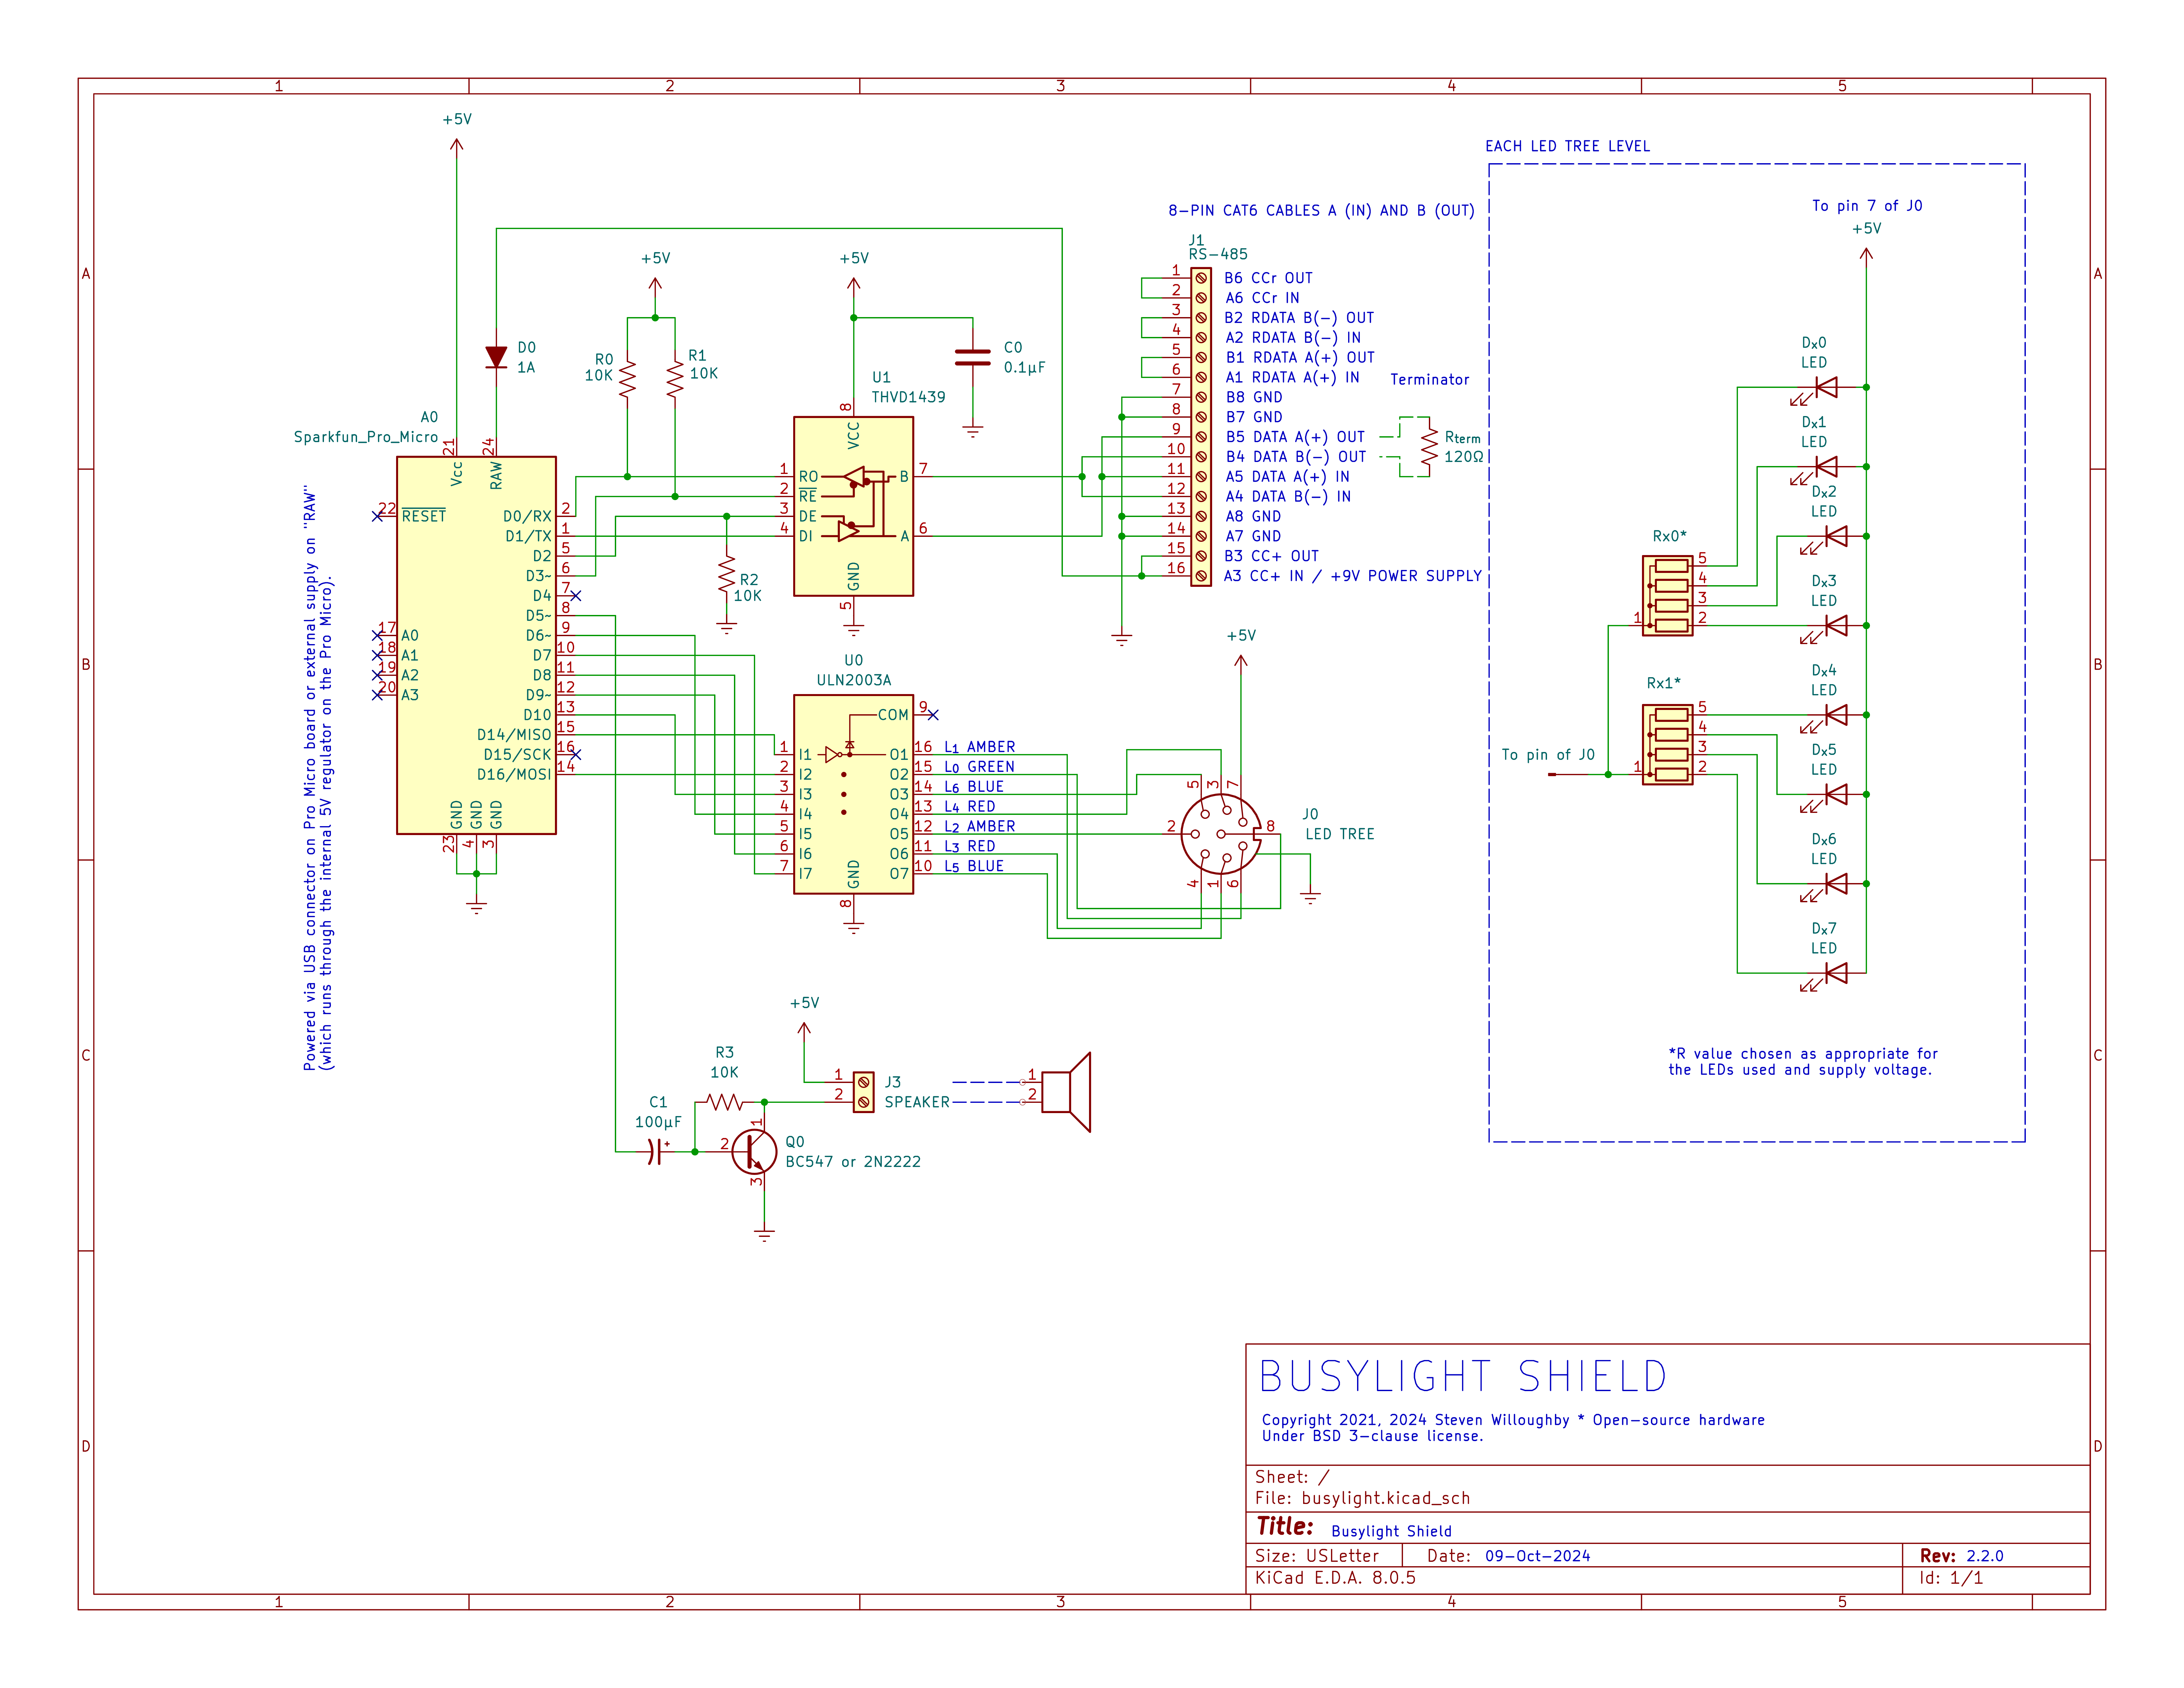
\includegraphics[width=\textheight,angle=90]{images/busylight_schematic.png}
\noindent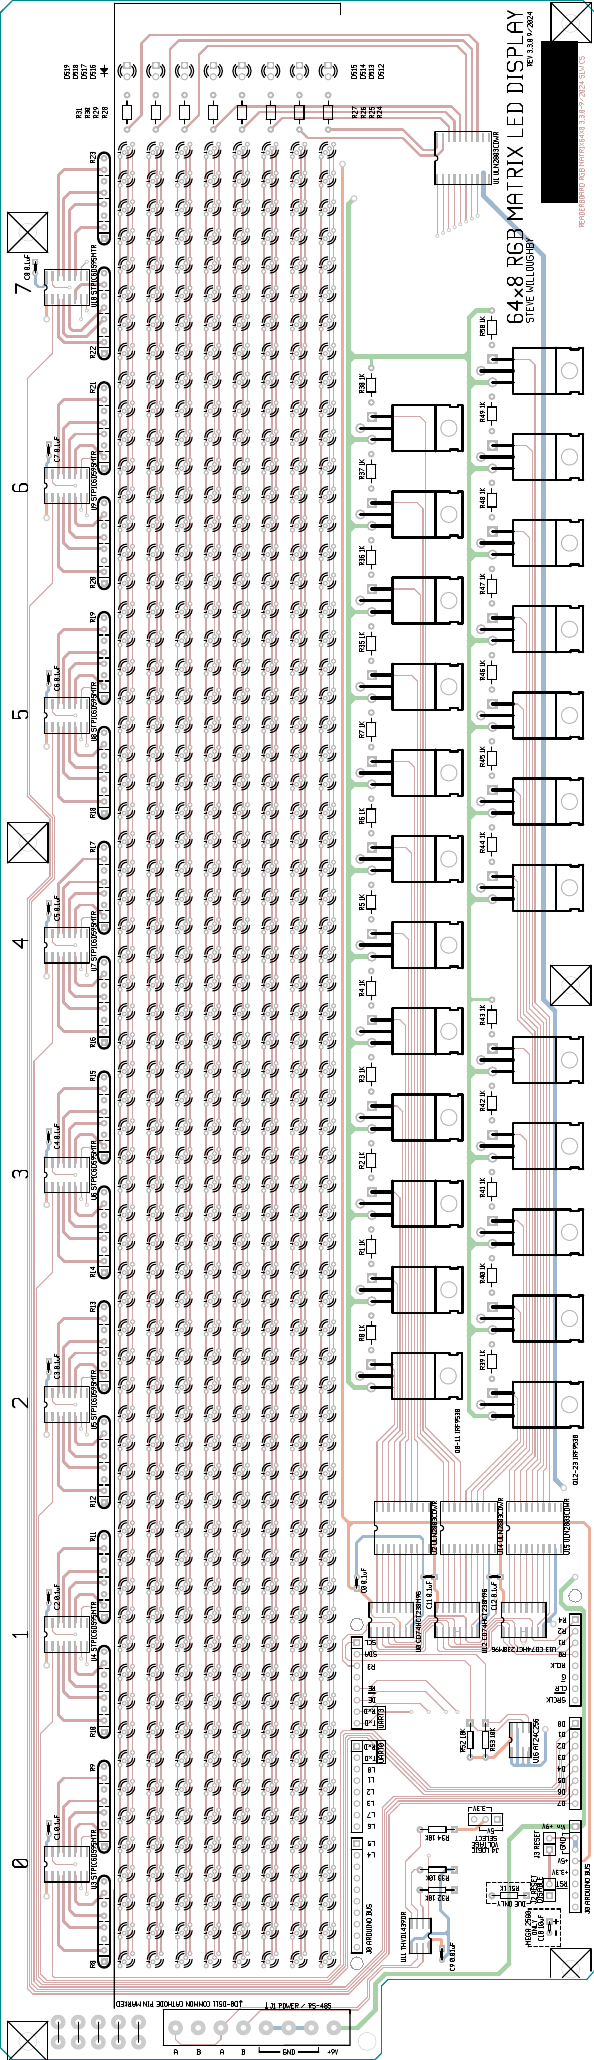
\includegraphics[height=\textheight]{images/readerboard-assembly-0.png}
\noindent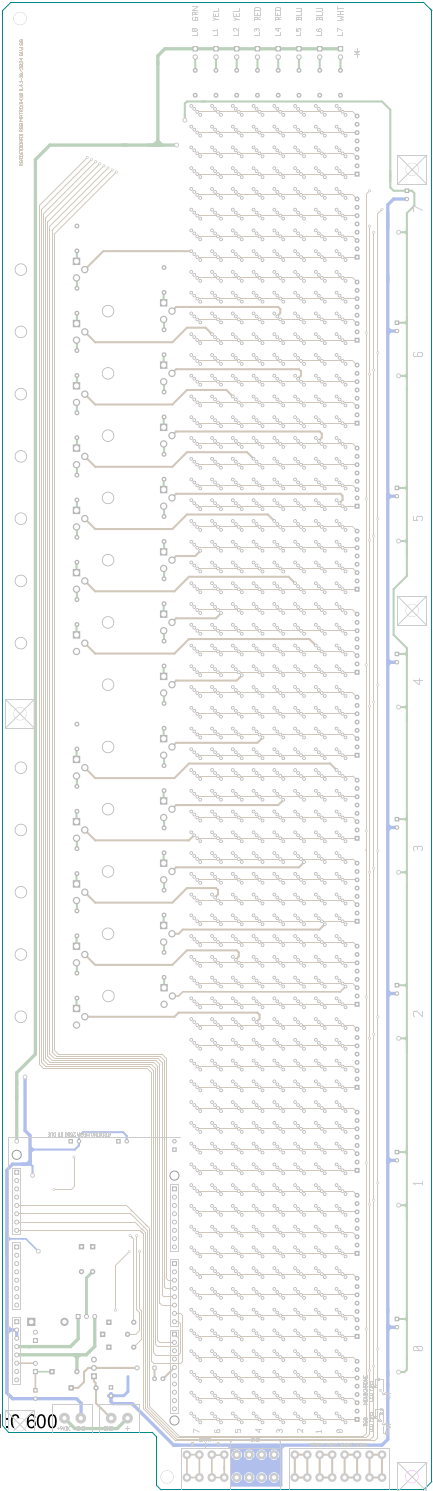
\includegraphics[height=\textheight]{images/readerboard-assembly-1.png}
\newpage
\noindent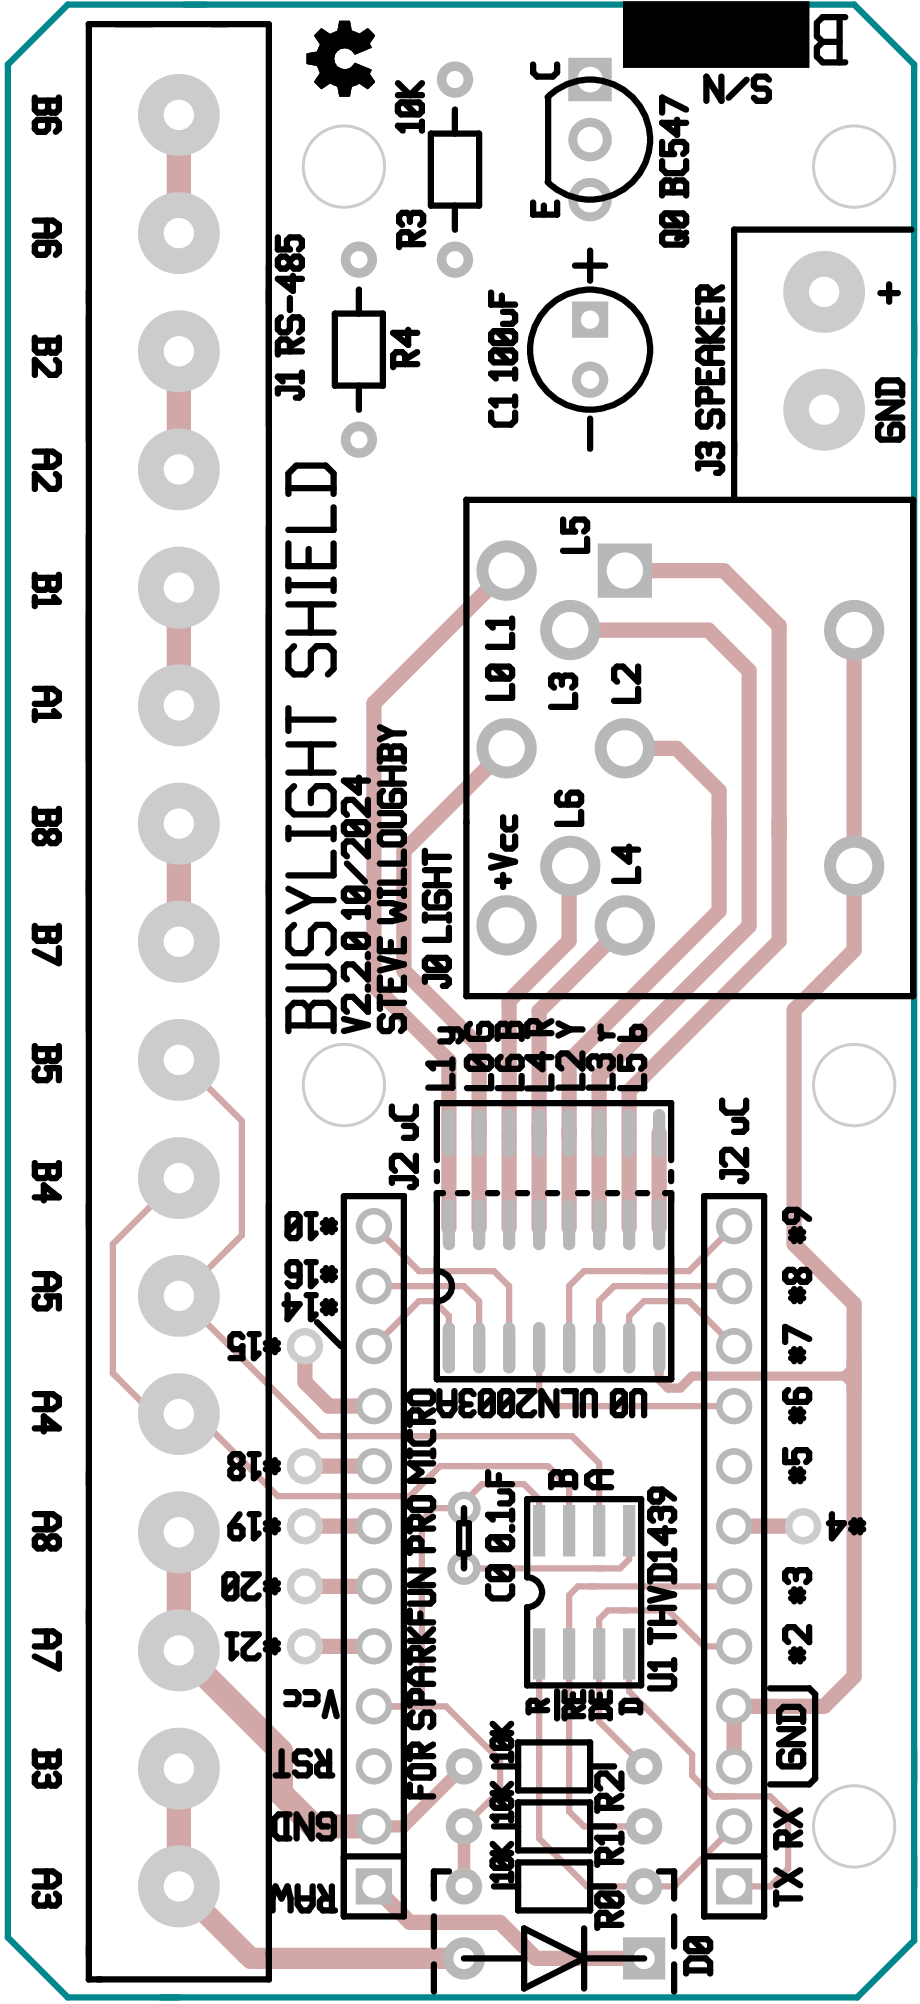
\includegraphics[width=.48\textwidth]{images/busylight_assembly-0.png}
\noindent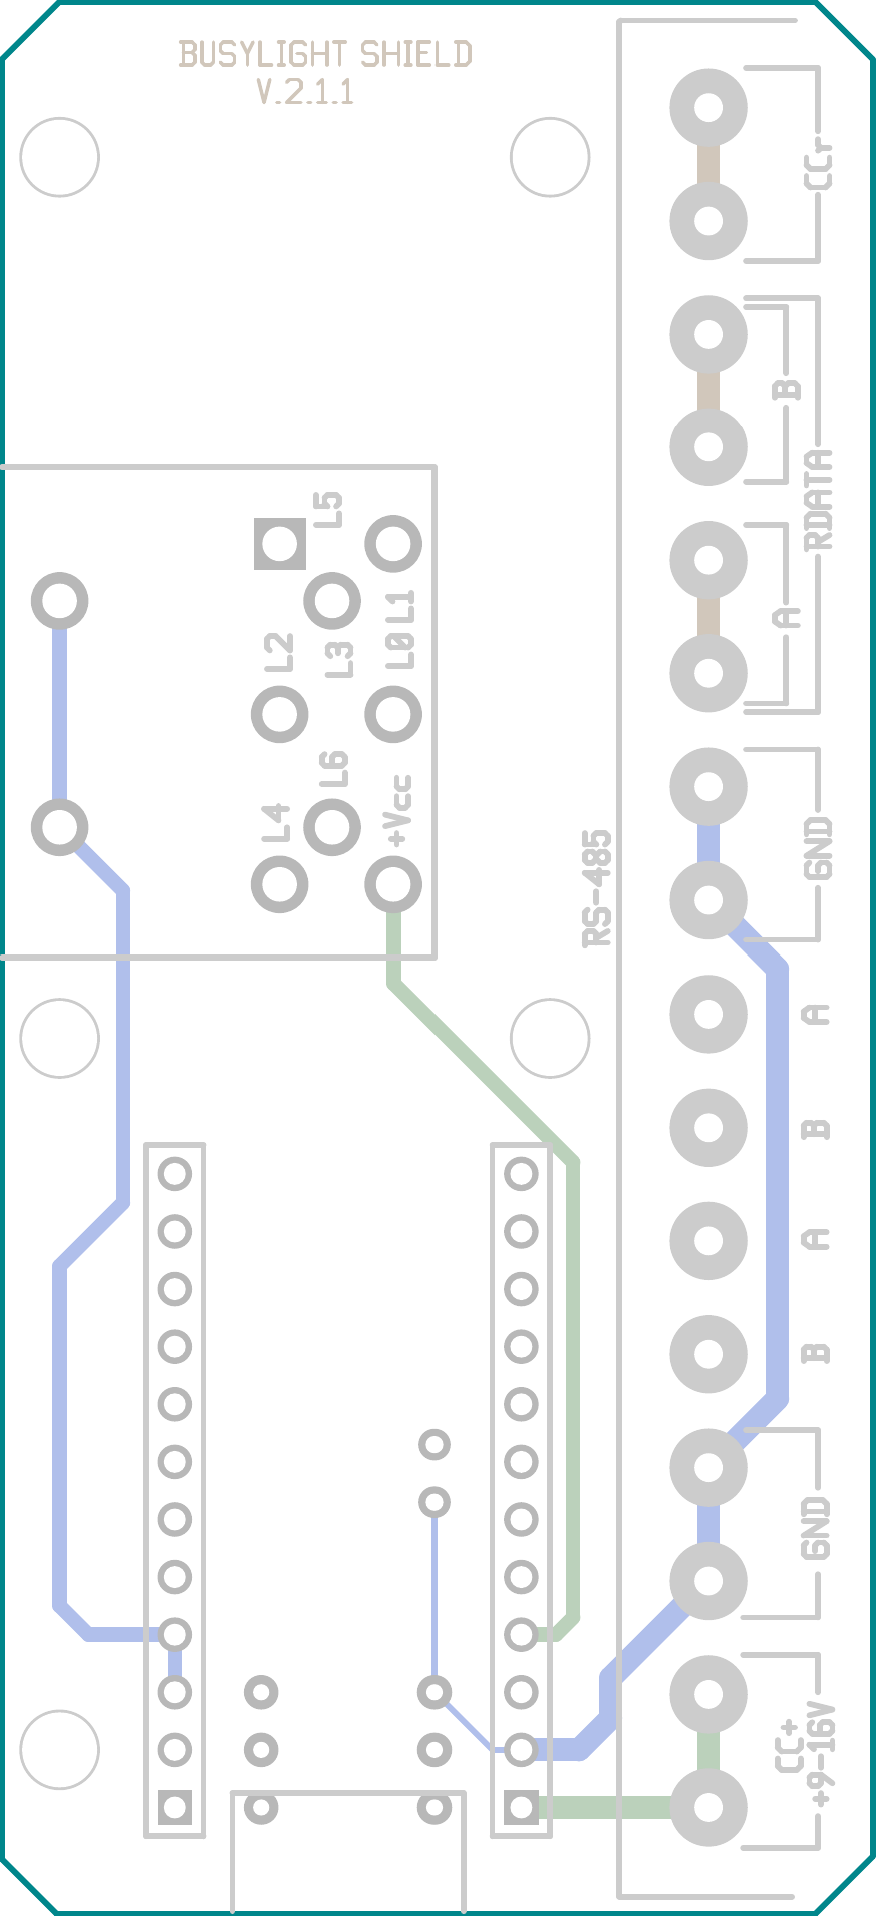
\includegraphics[width=.48\textwidth]{images/busylight_assembly-1.png}
\newpage
\noindent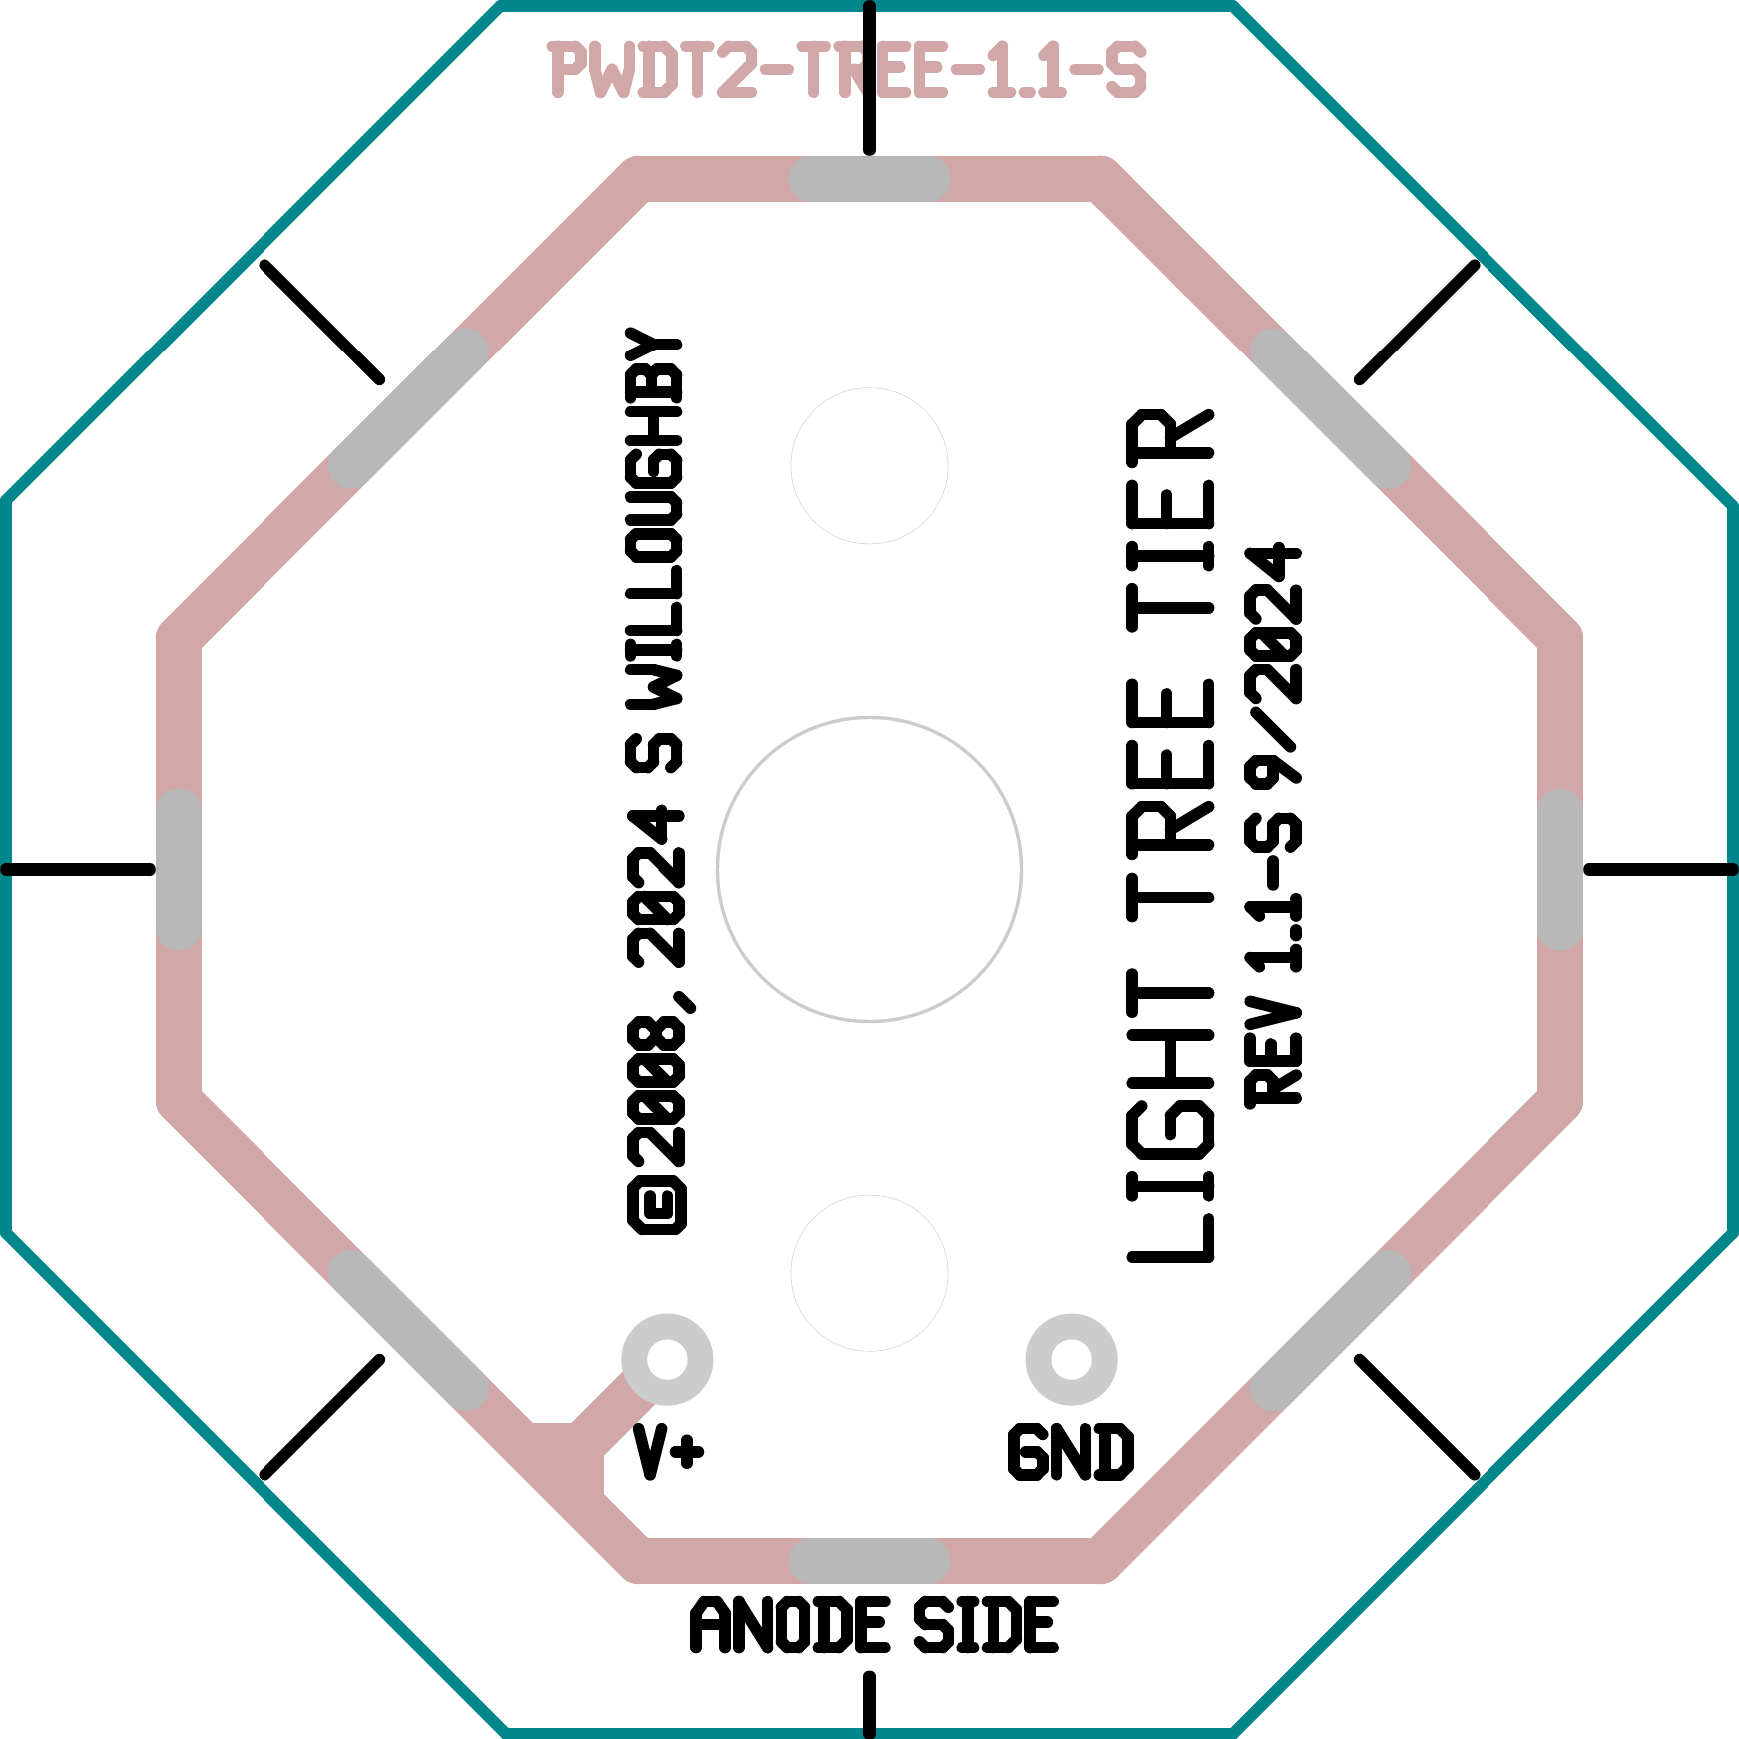
\includegraphics[width=.48\textwidth]{images/lighttree-assembly-0.png}
\noindent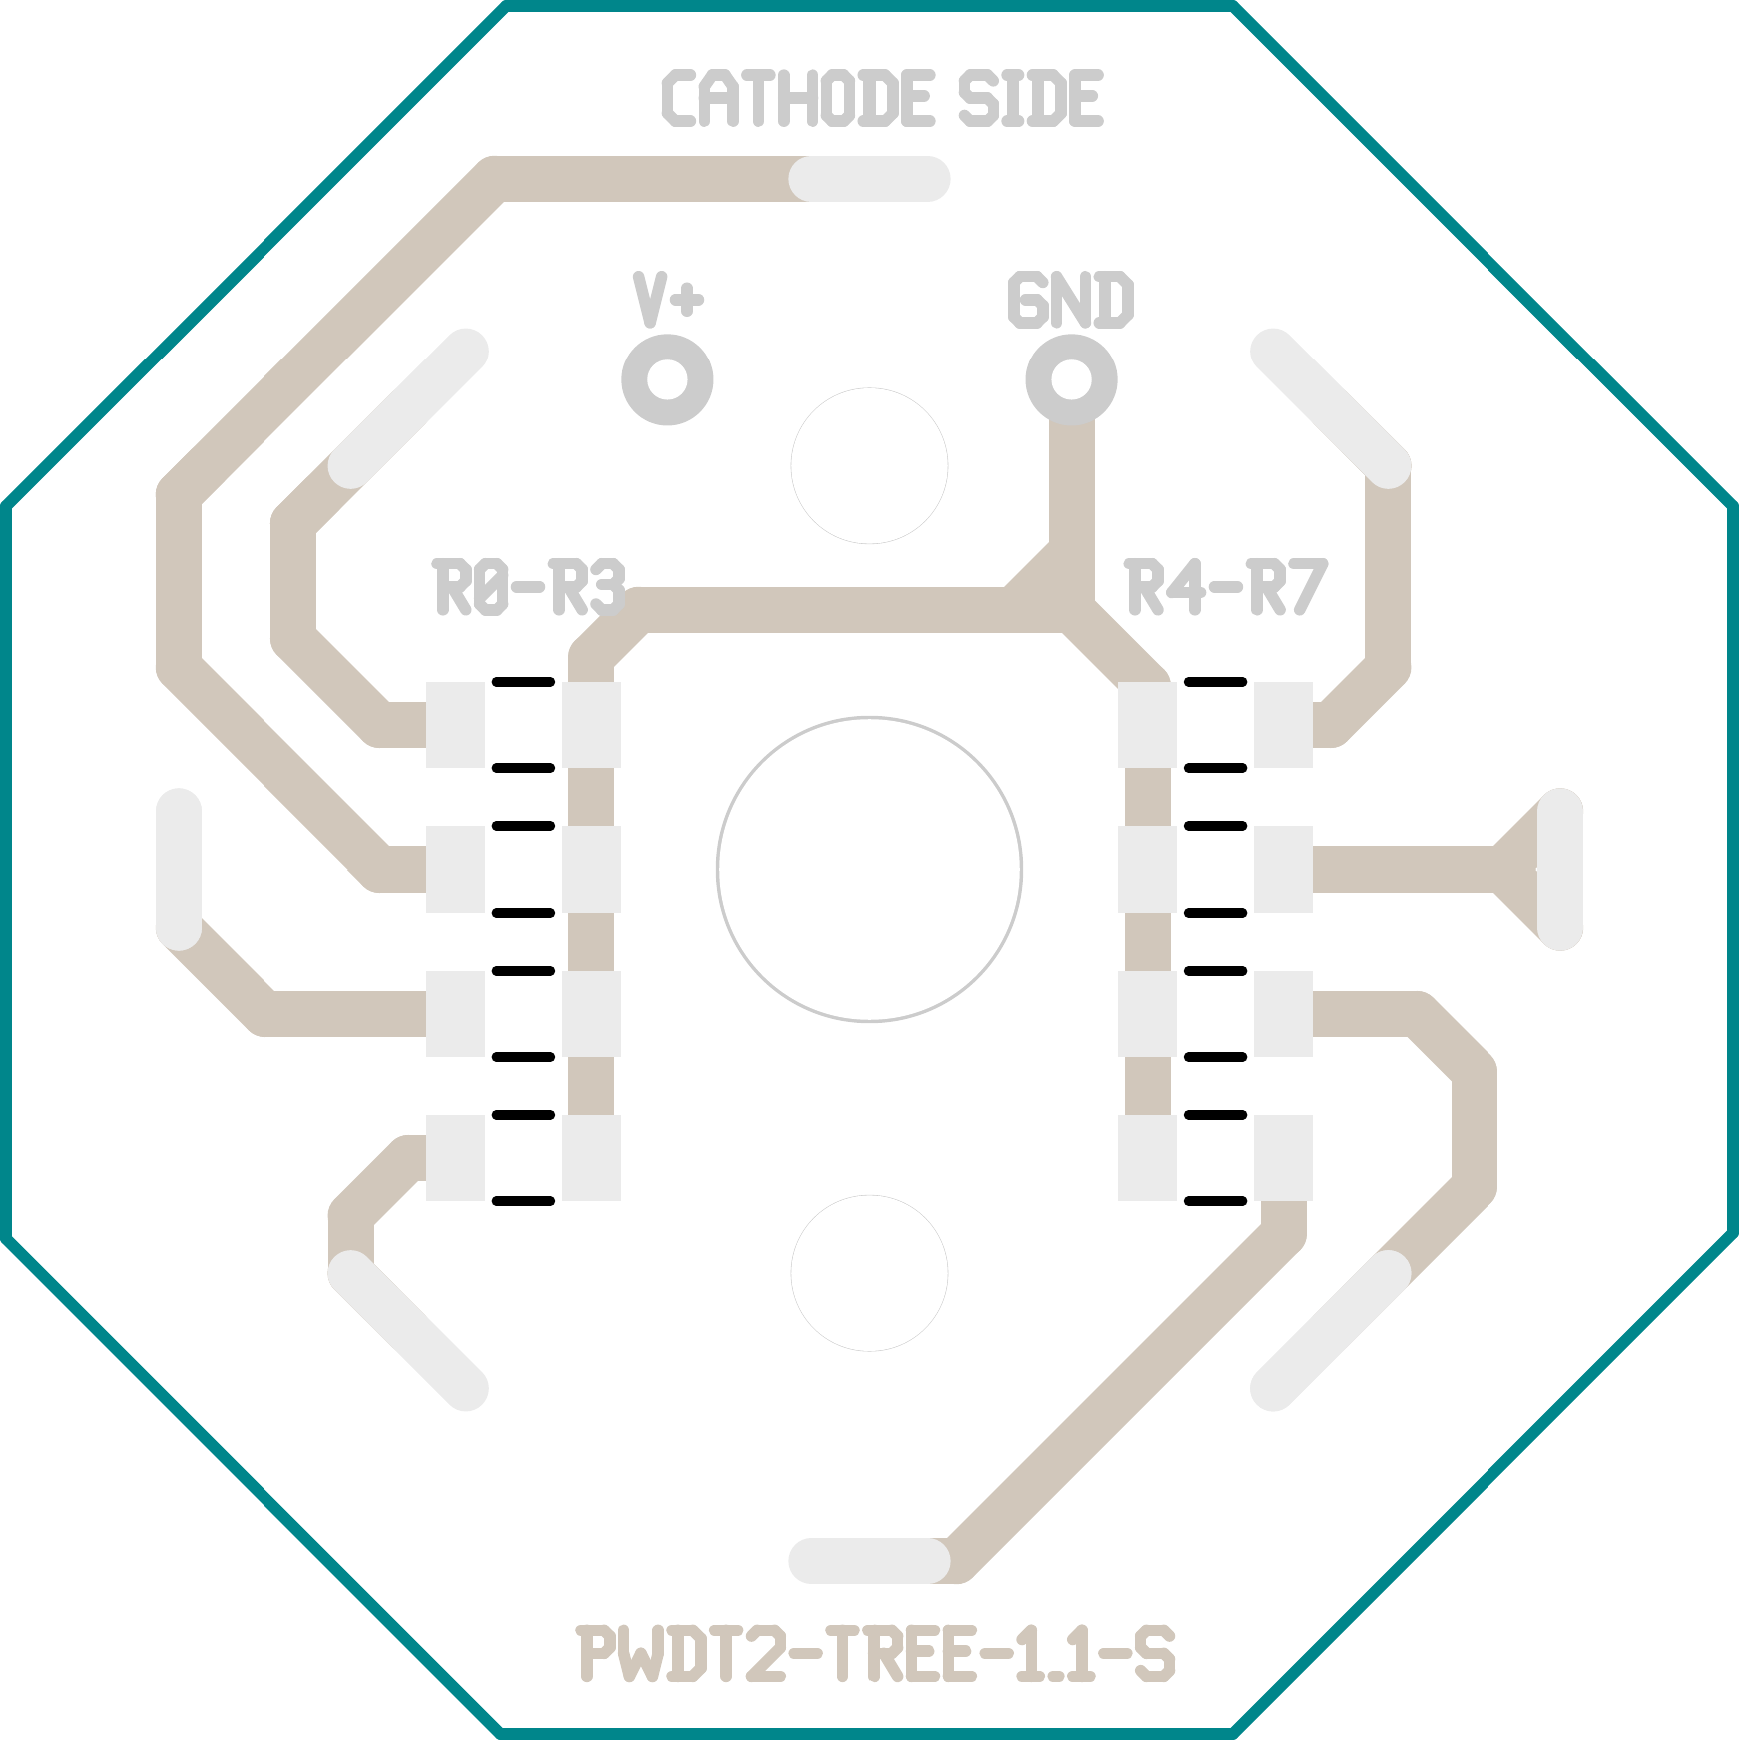
\includegraphics[width=.48\textwidth]{images/lighttree-assembly-1.png}

\noindent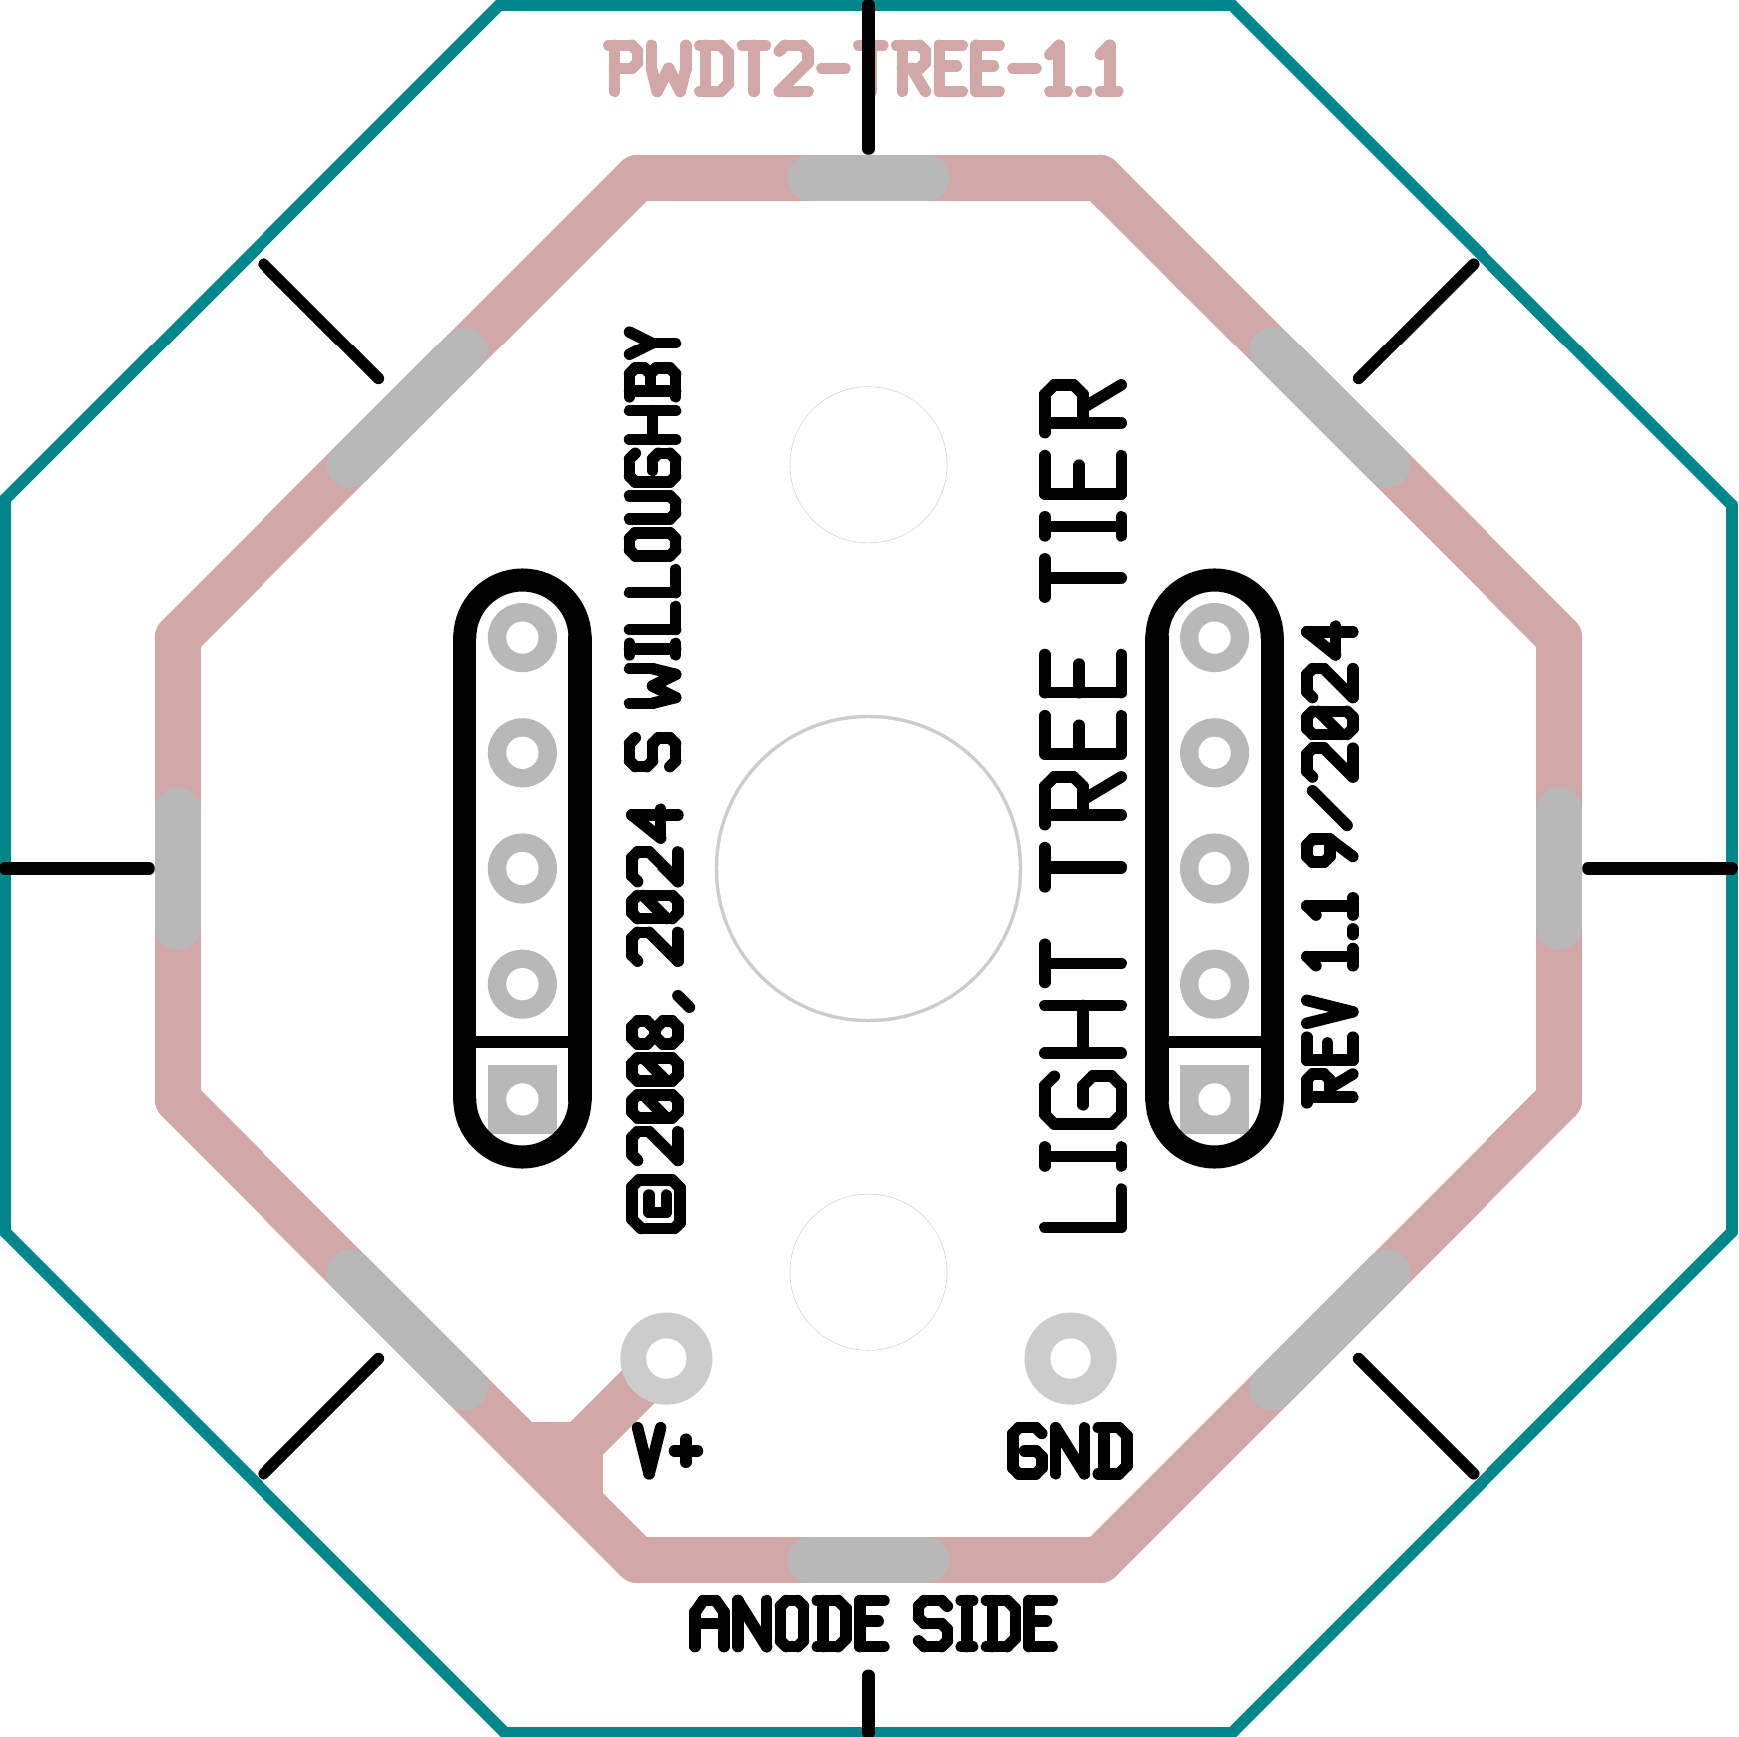
\includegraphics[width=.48\textwidth]{images/lighttree-assembly-S-0.png}
\noindent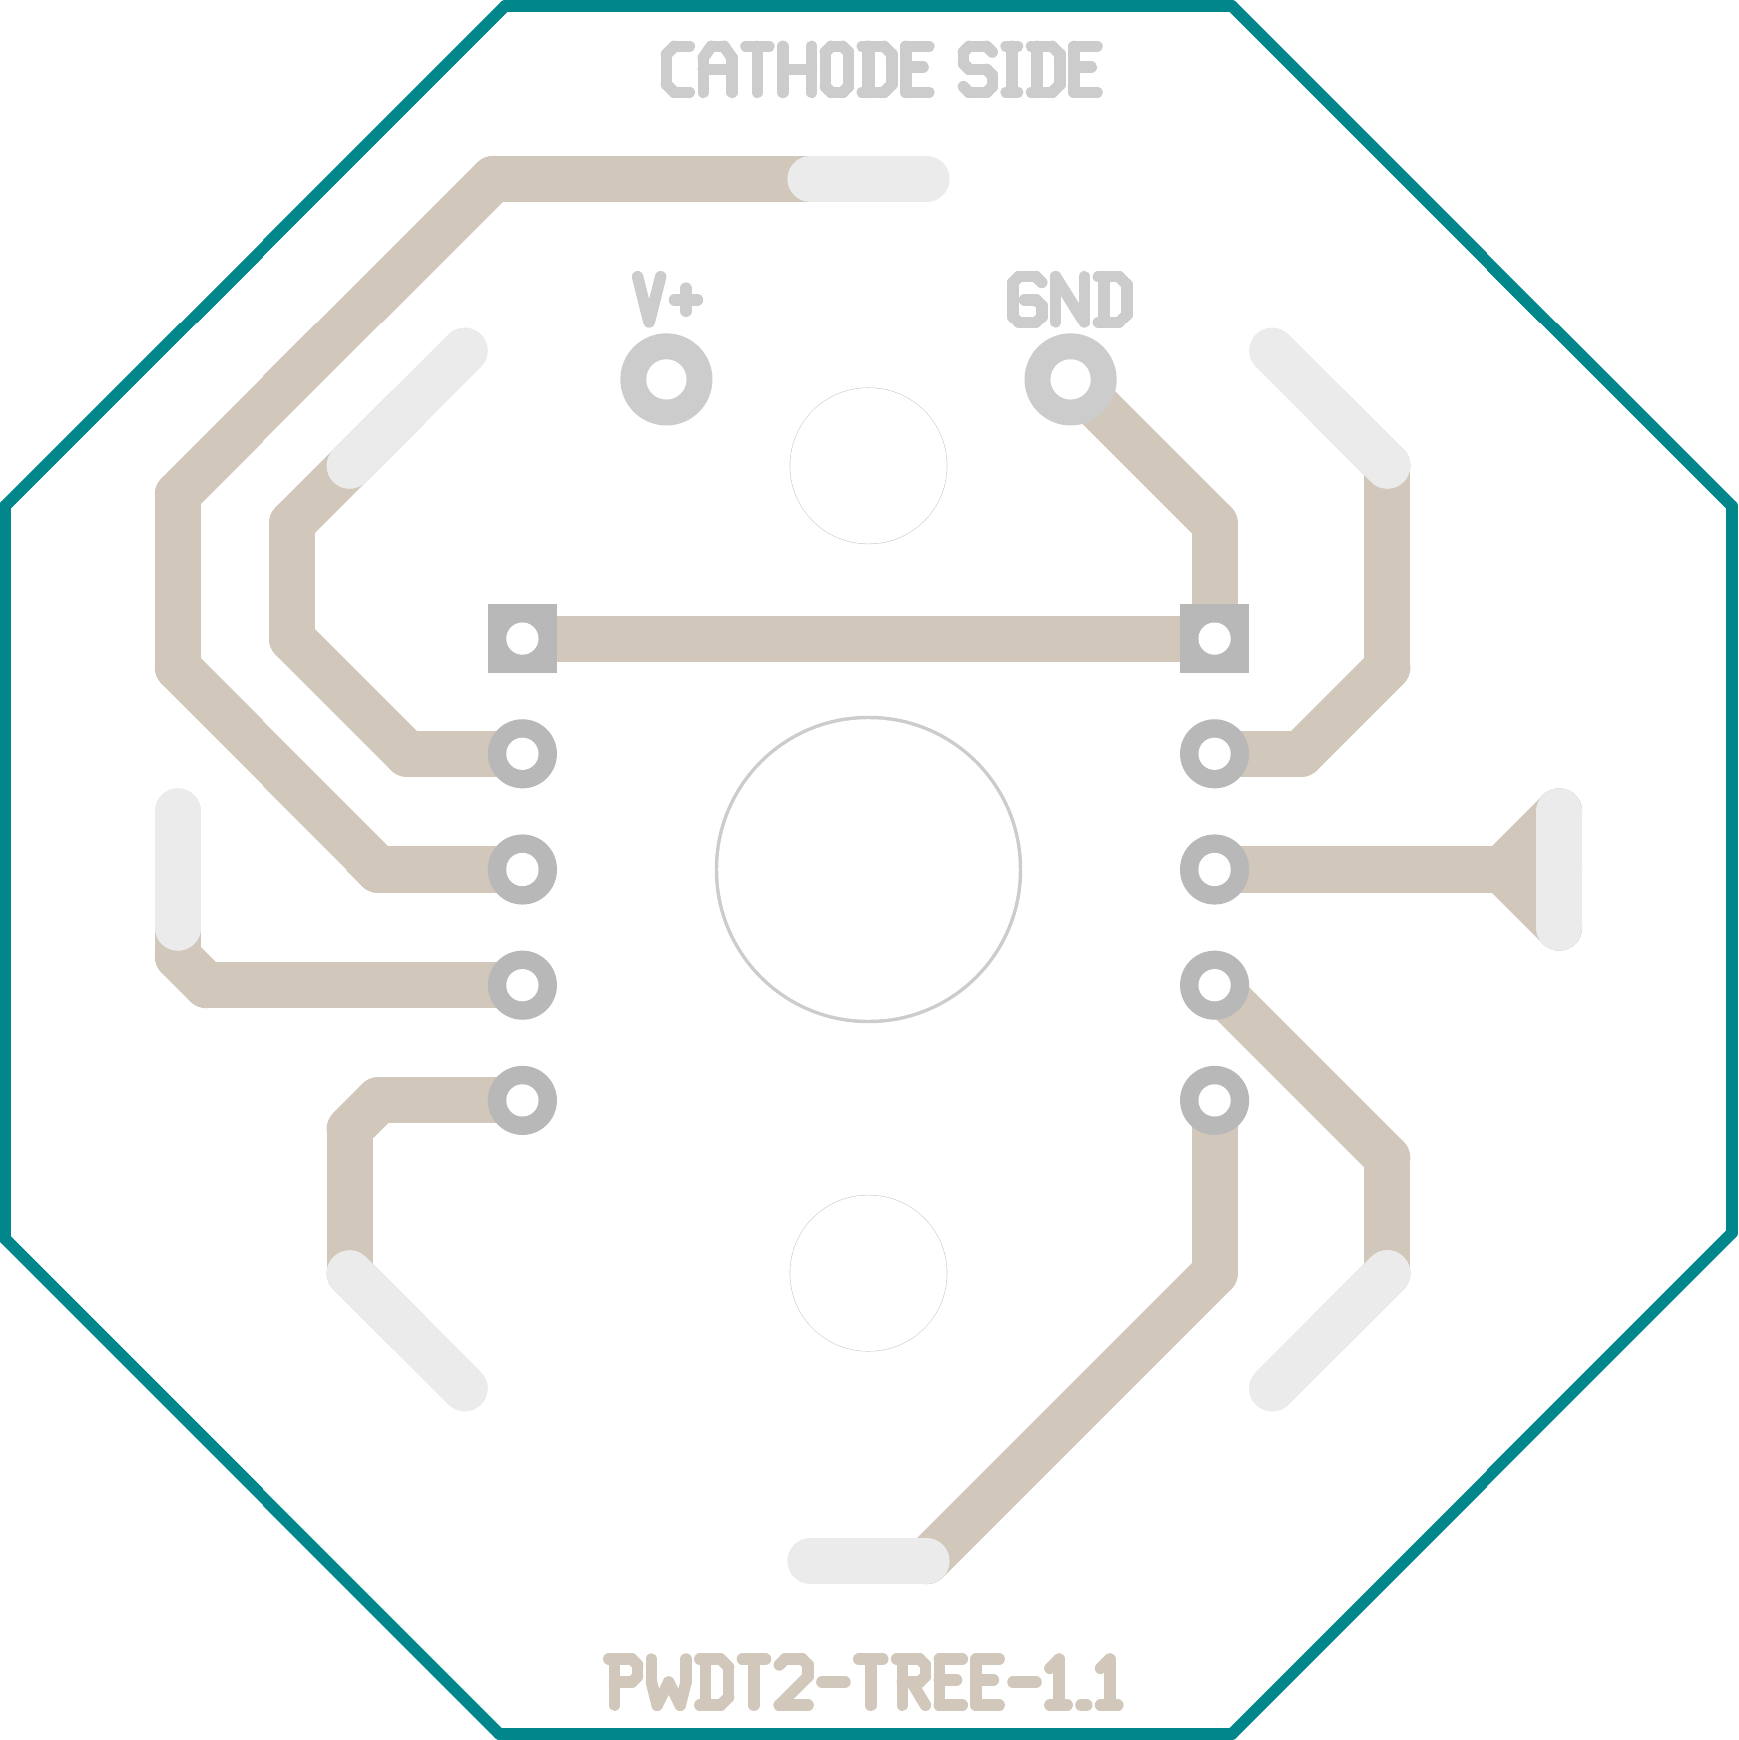
\includegraphics[width=.48\textwidth]{images/lighttree-assembly-S-1.png}
\indexintoc

\printindex
\end{document}
